% Options for packages loaded elsewhere
\PassOptionsToPackage{unicode}{hyperref}
\PassOptionsToPackage{hyphens}{url}
\PassOptionsToPackage{dvipsnames,svgnames,x11names}{xcolor}
%
\documentclass[
  letterpaper,
  DIV=11,
  numbers=noendperiod]{scrreprt}

\usepackage{amsmath,amssymb}
\usepackage{iftex}
\ifPDFTeX
  \usepackage[T1]{fontenc}
  \usepackage[utf8]{inputenc}
  \usepackage{textcomp} % provide euro and other symbols
\else % if luatex or xetex
  \usepackage{unicode-math}
  \defaultfontfeatures{Scale=MatchLowercase}
  \defaultfontfeatures[\rmfamily]{Ligatures=TeX,Scale=1}
\fi
\usepackage{lmodern}
\ifPDFTeX\else  
    % xetex/luatex font selection
\fi
% Use upquote if available, for straight quotes in verbatim environments
\IfFileExists{upquote.sty}{\usepackage{upquote}}{}
\IfFileExists{microtype.sty}{% use microtype if available
  \usepackage[]{microtype}
  \UseMicrotypeSet[protrusion]{basicmath} % disable protrusion for tt fonts
}{}
\makeatletter
\@ifundefined{KOMAClassName}{% if non-KOMA class
  \IfFileExists{parskip.sty}{%
    \usepackage{parskip}
  }{% else
    \setlength{\parindent}{0pt}
    \setlength{\parskip}{6pt plus 2pt minus 1pt}}
}{% if KOMA class
  \KOMAoptions{parskip=half}}
\makeatother
\usepackage{xcolor}
\setlength{\emergencystretch}{3em} % prevent overfull lines
\setcounter{secnumdepth}{1}
% Make \paragraph and \subparagraph free-standing
\ifx\paragraph\undefined\else
  \let\oldparagraph\paragraph
  \renewcommand{\paragraph}[1]{\oldparagraph{#1}\mbox{}}
\fi
\ifx\subparagraph\undefined\else
  \let\oldsubparagraph\subparagraph
  \renewcommand{\subparagraph}[1]{\oldsubparagraph{#1}\mbox{}}
\fi

\usepackage{color}
\usepackage{fancyvrb}
\newcommand{\VerbBar}{|}
\newcommand{\VERB}{\Verb[commandchars=\\\{\}]}
\DefineVerbatimEnvironment{Highlighting}{Verbatim}{commandchars=\\\{\}}
% Add ',fontsize=\small' for more characters per line
\usepackage{framed}
\definecolor{shadecolor}{RGB}{241,243,245}
\newenvironment{Shaded}{\begin{snugshade}}{\end{snugshade}}
\newcommand{\AlertTok}[1]{\textcolor[rgb]{0.68,0.00,0.00}{#1}}
\newcommand{\AnnotationTok}[1]{\textcolor[rgb]{0.37,0.37,0.37}{#1}}
\newcommand{\AttributeTok}[1]{\textcolor[rgb]{0.40,0.45,0.13}{#1}}
\newcommand{\BaseNTok}[1]{\textcolor[rgb]{0.68,0.00,0.00}{#1}}
\newcommand{\BuiltInTok}[1]{\textcolor[rgb]{0.00,0.23,0.31}{#1}}
\newcommand{\CharTok}[1]{\textcolor[rgb]{0.13,0.47,0.30}{#1}}
\newcommand{\CommentTok}[1]{\textcolor[rgb]{0.37,0.37,0.37}{#1}}
\newcommand{\CommentVarTok}[1]{\textcolor[rgb]{0.37,0.37,0.37}{\textit{#1}}}
\newcommand{\ConstantTok}[1]{\textcolor[rgb]{0.56,0.35,0.01}{#1}}
\newcommand{\ControlFlowTok}[1]{\textcolor[rgb]{0.00,0.23,0.31}{#1}}
\newcommand{\DataTypeTok}[1]{\textcolor[rgb]{0.68,0.00,0.00}{#1}}
\newcommand{\DecValTok}[1]{\textcolor[rgb]{0.68,0.00,0.00}{#1}}
\newcommand{\DocumentationTok}[1]{\textcolor[rgb]{0.37,0.37,0.37}{\textit{#1}}}
\newcommand{\ErrorTok}[1]{\textcolor[rgb]{0.68,0.00,0.00}{#1}}
\newcommand{\ExtensionTok}[1]{\textcolor[rgb]{0.00,0.23,0.31}{#1}}
\newcommand{\FloatTok}[1]{\textcolor[rgb]{0.68,0.00,0.00}{#1}}
\newcommand{\FunctionTok}[1]{\textcolor[rgb]{0.28,0.35,0.67}{#1}}
\newcommand{\ImportTok}[1]{\textcolor[rgb]{0.00,0.46,0.62}{#1}}
\newcommand{\InformationTok}[1]{\textcolor[rgb]{0.37,0.37,0.37}{#1}}
\newcommand{\KeywordTok}[1]{\textcolor[rgb]{0.00,0.23,0.31}{#1}}
\newcommand{\NormalTok}[1]{\textcolor[rgb]{0.00,0.23,0.31}{#1}}
\newcommand{\OperatorTok}[1]{\textcolor[rgb]{0.37,0.37,0.37}{#1}}
\newcommand{\OtherTok}[1]{\textcolor[rgb]{0.00,0.23,0.31}{#1}}
\newcommand{\PreprocessorTok}[1]{\textcolor[rgb]{0.68,0.00,0.00}{#1}}
\newcommand{\RegionMarkerTok}[1]{\textcolor[rgb]{0.00,0.23,0.31}{#1}}
\newcommand{\SpecialCharTok}[1]{\textcolor[rgb]{0.37,0.37,0.37}{#1}}
\newcommand{\SpecialStringTok}[1]{\textcolor[rgb]{0.13,0.47,0.30}{#1}}
\newcommand{\StringTok}[1]{\textcolor[rgb]{0.13,0.47,0.30}{#1}}
\newcommand{\VariableTok}[1]{\textcolor[rgb]{0.07,0.07,0.07}{#1}}
\newcommand{\VerbatimStringTok}[1]{\textcolor[rgb]{0.13,0.47,0.30}{#1}}
\newcommand{\WarningTok}[1]{\textcolor[rgb]{0.37,0.37,0.37}{\textit{#1}}}

\providecommand{\tightlist}{%
  \setlength{\itemsep}{0pt}\setlength{\parskip}{0pt}}\usepackage{longtable,booktabs,array}
\usepackage{calc} % for calculating minipage widths
% Correct order of tables after \paragraph or \subparagraph
\usepackage{etoolbox}
\makeatletter
\patchcmd\longtable{\par}{\if@noskipsec\mbox{}\fi\par}{}{}
\makeatother
% Allow footnotes in longtable head/foot
\IfFileExists{footnotehyper.sty}{\usepackage{footnotehyper}}{\usepackage{footnote}}
\makesavenoteenv{longtable}
\usepackage{graphicx}
\makeatletter
\def\maxwidth{\ifdim\Gin@nat@width>\linewidth\linewidth\else\Gin@nat@width\fi}
\def\maxheight{\ifdim\Gin@nat@height>\textheight\textheight\else\Gin@nat@height\fi}
\makeatother
% Scale images if necessary, so that they will not overflow the page
% margins by default, and it is still possible to overwrite the defaults
% using explicit options in \includegraphics[width, height, ...]{}
\setkeys{Gin}{width=\maxwidth,height=\maxheight,keepaspectratio}
% Set default figure placement to htbp
\makeatletter
\def\fps@figure{htbp}
\makeatother

\KOMAoption{captions}{tableheading}
\makeatletter
\@ifpackageloaded{bookmark}{}{\usepackage{bookmark}}
\makeatother
\makeatletter
\@ifpackageloaded{caption}{}{\usepackage{caption}}
\AtBeginDocument{%
\ifdefined\contentsname
  \renewcommand*\contentsname{Table of contents}
\else
  \newcommand\contentsname{Table of contents}
\fi
\ifdefined\listfigurename
  \renewcommand*\listfigurename{List of Figures}
\else
  \newcommand\listfigurename{List of Figures}
\fi
\ifdefined\listtablename
  \renewcommand*\listtablename{List of Tables}
\else
  \newcommand\listtablename{List of Tables}
\fi
\ifdefined\figurename
  \renewcommand*\figurename{Figure}
\else
  \newcommand\figurename{Figure}
\fi
\ifdefined\tablename
  \renewcommand*\tablename{Table}
\else
  \newcommand\tablename{Table}
\fi
}
\@ifpackageloaded{float}{}{\usepackage{float}}
\floatstyle{ruled}
\@ifundefined{c@chapter}{\newfloat{codelisting}{h}{lop}}{\newfloat{codelisting}{h}{lop}[chapter]}
\floatname{codelisting}{Listing}
\newcommand*\listoflistings{\listof{codelisting}{List of Listings}}
\makeatother
\makeatletter
\makeatother
\makeatletter
\@ifpackageloaded{caption}{}{\usepackage{caption}}
\@ifpackageloaded{subcaption}{}{\usepackage{subcaption}}
\makeatother
\ifLuaTeX
  \usepackage{selnolig}  % disable illegal ligatures
\fi
\usepackage{bookmark}

\IfFileExists{xurl.sty}{\usepackage{xurl}}{} % add URL line breaks if available
\urlstyle{same} % disable monospaced font for URLs
\hypersetup{
  pdftitle={R Code for `A Practical Guide . . .'},
  pdfauthor={John Maindonald},
  colorlinks=true,
  linkcolor={blue},
  filecolor={Maroon},
  citecolor={Blue},
  urlcolor={Blue},
  pdfcreator={LaTeX via pandoc}}

\title{R Code for `A Practical Guide . . .'}
\author{John Maindonald}
\date{2024-06-08}

\begin{document}
\maketitle

\renewcommand*\contentsname{Table of contents}
{
\hypersetup{linkcolor=}
\setcounter{tocdepth}{2}
\tableofcontents
}
\bookmarksetup{startatroot}

\chapter*{Preface}\label{preface}
\addcontentsline{toc}{chapter}{Preface}

\markboth{Preface}{Preface}

Code provided here is for the May 2024 text:

\begin{quote}
``A Practical Guide to Data Analysis Using R -- An Example-Based
Approach'', by John H Maindonald, W John Braun, and Jeffrey L Andrews.
\end{quote}

Code that is shown in the text is filled out to include all code for
graphs. In chapter 2 and later, the text includes code only for those
graphs that are specifically targeted at the methodology under
discussion.

The text has been available in digital format since early May 2024. It
has been available in print in the UK from May 30, is due to be
available in print in the USA in July, and in Australia and New Zealand
in August 2024.

For details for the UK, see:
\href{https://www.cambridge.org/gb/universitypress/subjects/statistics-probability/computational-statistics-machine-learning-and-information-sc/practical-guide-data-analysis-using-r-example-based-approach}{A
Practical Guide to Data Analysis Using R -- Cambridge University Press
UK}

\bookmarksetup{startatroot}

\chapter{Chapter 1: Learning from
data}\label{chapter-1-learning-from-data}

\begin{Shaded}
\begin{Highlighting}[]
\FunctionTok{library}\NormalTok{(knitr)}
\NormalTok{opts\_chunk[[}\StringTok{\textquotesingle{}set\textquotesingle{}}\NormalTok{]](}\AttributeTok{fig.width=}\DecValTok{6}\NormalTok{, }\AttributeTok{fig.height=}\DecValTok{6}\NormalTok{, }\AttributeTok{comment=}\StringTok{" "}\NormalTok{,}
                    \AttributeTok{out.width=}\StringTok{"80\%"}\NormalTok{, }\AttributeTok{fig.align=}\StringTok{"center"}\NormalTok{, }\AttributeTok{fig.show=}\StringTok{\textquotesingle{}hold\textquotesingle{}}\NormalTok{,}
                    \AttributeTok{size=}\StringTok{"small"}\NormalTok{, }\AttributeTok{ps=}\DecValTok{10}\NormalTok{, }\AttributeTok{strip.white =} \ConstantTok{TRUE}\NormalTok{, }
                    \AttributeTok{tidy.opts =} \FunctionTok{list}\NormalTok{(}\AttributeTok{replace.assign=}\ConstantTok{FALSE}\NormalTok{))}
\end{Highlighting}
\end{Shaded}

\begin{Shaded}
\begin{Highlighting}[]
\DocumentationTok{\#\# xtras=TRUE    \#\# Set to TRUE to execute code \textquotesingle{}extras\textquotesingle{}}
\NormalTok{xtras }\OtherTok{\textless{}{-}} \ConstantTok{FALSE}
\FunctionTok{library}\NormalTok{(knitr)}
\DocumentationTok{\#\# opts\_chunk[[\textquotesingle{}set\textquotesingle{}]](results="asis")}
\DocumentationTok{\#\# opts\_chunk[[\textquotesingle{}set\textquotesingle{}]](eval=FALSE)   \#\# Set to TRUE to execute main part of code}
\NormalTok{opts\_chunk[[}\StringTok{\textquotesingle{}set\textquotesingle{}}\NormalTok{]](}\AttributeTok{eval=}\ConstantTok{FALSE}\NormalTok{) }
\end{Highlighting}
\end{Shaded}

\paragraph{Packages required (plus any
dependencies)}\label{packages-required-plus-any-dependencies}

latticeExtra (lattice is a dependency); DAAG; car; MASS; AICcmodavg;
BayesFactor; boot; MPV; ggplot2; tidyr

Additionally, knitr and Hmisc are required in order to process the Rmd
source file. The prettydoc package is by default used to format the html
output.

\paragraph{Chapter summary}\label{chapter-summary}

\paragraph{A note on terminology --- variables, factors, and
more!}\label{a-note-on-terminology-variables-factors-and-more}

\subsection{Section 1.1: Questions, and data that may point to
answers}\label{section-1.1-questions-and-data-that-may-point-to-answers}

\subsubsection{Subsection 1.1.1: A sample is a window into the wider
population}\label{subsection-1.1.1-a-sample-is-a-window-into-the-wider-population}

\begin{Shaded}
\begin{Highlighting}[]
\DocumentationTok{\#\# For the sequence below, precede with set.seed(3676)}
\FunctionTok{set.seed}\NormalTok{(}\DecValTok{3696}\NormalTok{)}
\FunctionTok{sample}\NormalTok{(}\DecValTok{1}\SpecialCharTok{:}\DecValTok{9384}\NormalTok{, }\DecValTok{12}\NormalTok{, }\AttributeTok{replace=}\ConstantTok{FALSE}\NormalTok{)  }\CommentTok{\# NB: \textasciigrave{}replace=FALSE\textasciigrave{} is the default}
\end{Highlighting}
\end{Shaded}

\begin{Shaded}
\begin{Highlighting}[]
\NormalTok{chosen1200 }\OtherTok{\textless{}{-}} \FunctionTok{sample}\NormalTok{(}\DecValTok{1}\SpecialCharTok{:}\DecValTok{19384}\NormalTok{, }\DecValTok{1200}\NormalTok{, }\AttributeTok{replace=}\ConstantTok{FALSE}\NormalTok{)  }
\end{Highlighting}
\end{Shaded}

\begin{Shaded}
\begin{Highlighting}[]
\DocumentationTok{\#\# For the sequence below, precede with set.seed(366)}
\FunctionTok{set.seed}\NormalTok{(}\DecValTok{366}\NormalTok{)}
\FunctionTok{split}\NormalTok{(}\FunctionTok{sample}\NormalTok{(}\FunctionTok{seq}\NormalTok{(}\DecValTok{1}\SpecialCharTok{:}\DecValTok{10}\NormalTok{)), }\FunctionTok{rep}\NormalTok{(}\FunctionTok{c}\NormalTok{(}\StringTok{"Control"}\NormalTok{,}\StringTok{"Treatment"}\NormalTok{), }\DecValTok{5}\NormalTok{))}
\CommentTok{\# sample(1:10) gives a random re{-}arrangement (permutation) of 1, 2, ..., 10}
\end{Highlighting}
\end{Shaded}

\paragraph{Cluster sampling}\label{cluster-sampling}

\paragraph{*A note on with-replacement
samples}\label{a-note-on-with-replacement-samples}

\begin{Shaded}
\begin{Highlighting}[]
\FunctionTok{sample}\NormalTok{(}\DecValTok{1}\SpecialCharTok{:}\DecValTok{10}\NormalTok{, }\AttributeTok{replace=}\ConstantTok{TRUE}\NormalTok{)}
\DocumentationTok{\#\# sample(1:10, replace=FALSE) returns a random permutation of 1,2,...10}
\end{Highlighting}
\end{Shaded}

\subsubsection{Subsection 1.1.2: Formulating the scientific
question}\label{subsection-1.1.2-formulating-the-scientific-question}

\paragraph{Example: a question about cuckoo
eggs}\label{example-a-question-about-cuckoo-eggs}

\begin{Shaded}
\begin{Highlighting}[]
\FunctionTok{library}\NormalTok{(latticeExtra)   }\CommentTok{\# Lattice package will be loaded and attached also}
\NormalTok{cuckoos }\OtherTok{\textless{}{-}}\NormalTok{ DAAG}\SpecialCharTok{::}\NormalTok{cuckoos}
\DocumentationTok{\#\# Panel A: Dotplot without species means added}
\FunctionTok{dotplot}\NormalTok{(species }\SpecialCharTok{\textasciitilde{}}\NormalTok{ length, }\AttributeTok{data=}\NormalTok{cuckoos)   }\DocumentationTok{\#\# \textasciigrave{}species \textasciitilde{} length\textasciigrave{} is a \textquotesingle{}formula\textquotesingle{}}
\DocumentationTok{\#\# Panel B: Box and whisker plot}
\FunctionTok{bwplot}\NormalTok{(species }\SpecialCharTok{\textasciitilde{}}\NormalTok{ length, }\AttributeTok{data=}\NormalTok{cuckoos)}
\DocumentationTok{\#\# The following shows Panel A, including species means \& other tweaks}
\NormalTok{av }\OtherTok{\textless{}{-}} \FunctionTok{with}\NormalTok{(cuckoos, }\FunctionTok{aggregate}\NormalTok{(length, }\FunctionTok{list}\NormalTok{(}\AttributeTok{species=}\NormalTok{species), }\AttributeTok{FUN=}\NormalTok{mean))}
\FunctionTok{dotplot}\NormalTok{(species }\SpecialCharTok{\textasciitilde{}}\NormalTok{ length, }\AttributeTok{data=}\NormalTok{cuckoos, }\AttributeTok{alpha=}\FloatTok{0.4}\NormalTok{, }\AttributeTok{xlab=}\StringTok{"Length of egg (mm)"}\NormalTok{) }\SpecialCharTok{+}
  \FunctionTok{as.layer}\NormalTok{(}\FunctionTok{dotplot}\NormalTok{(species }\SpecialCharTok{\textasciitilde{}}\NormalTok{ x, }\AttributeTok{pch=}\DecValTok{3}\NormalTok{, }\AttributeTok{cex=}\FloatTok{1.4}\NormalTok{, }\AttributeTok{col=}\StringTok{"black"}\NormalTok{, }\AttributeTok{data=}\NormalTok{av))}
  \CommentTok{\# Use \textasciigrave{}+\textasciigrave{} to indicate that more (another \textquotesingle{}layer\textquotesingle{}) is to be added.}
  \CommentTok{\# With \textasciigrave{}alpha=0.4\textasciigrave{}, 40\% is the point color with 60\% background color}
  \CommentTok{\# \textasciigrave{}pch=3\textasciigrave{}: Plot character 3 is \textquotesingle{}+\textquotesingle{}; \textasciigrave{}cex=1.4\textasciigrave{}: Default char size X 1.4}
\end{Highlighting}
\end{Shaded}

\begin{Shaded}
\begin{Highlighting}[]
\DocumentationTok{\#\# Code}
\FunctionTok{suppressPackageStartupMessages}\NormalTok{(}\FunctionTok{library}\NormalTok{(latticeExtra, }\AttributeTok{quietly=}\ConstantTok{TRUE}\NormalTok{))}
\NormalTok{cuckoos }\OtherTok{\textless{}{-}}\NormalTok{ DAAG}\SpecialCharTok{::}\NormalTok{cuckoos}
\DocumentationTok{\#\# For tidier labels replace ".", in several of the names, by a space}
\NormalTok{specnam }\OtherTok{\textless{}{-}} \FunctionTok{with}\NormalTok{(cuckoos, }\FunctionTok{sub}\NormalTok{(}\AttributeTok{pattern=}\StringTok{"."}\NormalTok{, }\AttributeTok{replacement=}\StringTok{" "}\NormalTok{, }
                             \FunctionTok{levels}\NormalTok{(species), }\AttributeTok{fixed=}\ConstantTok{TRUE}\NormalTok{))}
\CommentTok{\# fixed=TRUE: "interpret "." as ".", not as a \textquotesingle{}any single character\textquotesingle{}"}
\NormalTok{cuckoos }\OtherTok{\textless{}{-}} \FunctionTok{within}\NormalTok{(cuckoos, }\FunctionTok{levels}\NormalTok{(species) }\OtherTok{\textless{}{-}}\NormalTok{ specnam)}
\DocumentationTok{\#\# Panel A: Dotplot: data frame cuckoos (DAAG)}
\NormalTok{av }\OtherTok{\textless{}{-}} \FunctionTok{with}\NormalTok{(cuckoos, }\FunctionTok{aggregate}\NormalTok{(length, }\FunctionTok{list}\NormalTok{(}\AttributeTok{species=}\NormalTok{species), }\AttributeTok{FUN=}\NormalTok{mean))}
\NormalTok{gphA }\OtherTok{\textless{}{-}} \FunctionTok{dotplot}\NormalTok{(species }\SpecialCharTok{\textasciitilde{}}\NormalTok{ length, }\AttributeTok{data=}\NormalTok{cuckoos, }\AttributeTok{alpha=}\FloatTok{0.4}\NormalTok{) }\SpecialCharTok{+}
  \FunctionTok{as.layer}\NormalTok{(}\FunctionTok{dotplot}\NormalTok{(species }\SpecialCharTok{\textasciitilde{}}\NormalTok{ x, }\AttributeTok{pch=}\DecValTok{3}\NormalTok{, }\AttributeTok{cex=}\FloatTok{1.4}\NormalTok{, }\AttributeTok{col=}\StringTok{"black"}\NormalTok{, }\AttributeTok{data=}\NormalTok{av))}
\CommentTok{\# alpha sets opacity. With alpha=0.4, 60\% of the background shows through}
\CommentTok{\# Enter \textasciigrave{}print(plt1)\textasciigrave{} or \textasciigrave{}plot(plt1)\textasciigrave{} or simply \textasciigrave{}plt1\textasciigrave{} to display the graph}
\DocumentationTok{\#\# Panel B: Box plot}
\NormalTok{gphB }\OtherTok{\textless{}{-}} \FunctionTok{bwplot}\NormalTok{(species }\SpecialCharTok{\textasciitilde{}}\NormalTok{ length, }\AttributeTok{data=}\NormalTok{cuckoos)}
\FunctionTok{update}\NormalTok{(}\FunctionTok{c}\NormalTok{(}\StringTok{"A: Dotplot"}\OtherTok{=}\NormalTok{gphA, }\StringTok{"B: Boxplot"}\OtherTok{=}\NormalTok{gphB), }\AttributeTok{between=}\FunctionTok{list}\NormalTok{(}\AttributeTok{x=}\FloatTok{0.4}\NormalTok{),}
       \AttributeTok{xlab=}\StringTok{"Length of egg (mm)"}\NormalTok{) }
\DocumentationTok{\#\# latticeExtra::c() joins compatible plots together. }
\DocumentationTok{\#\#   See \textasciigrave{}?latticeExtra::c\textasciigrave{}}
\end{Highlighting}
\end{Shaded}

\subsubsection{Subsection 1.1.3: Planning for a statistical
analysis}\label{subsection-1.1.3-planning-for-a-statistical-analysis}

\paragraph{Understand the data}\label{understand-the-data}

\paragraph{Causal inference}\label{causal-inference}

\paragraph{What was measured? Is it the relevant
measure?}\label{what-was-measured-is-it-the-relevant-measure}

\paragraph{Use relevant prior information in the planning
stages}\label{use-relevant-prior-information-in-the-planning-stages}

\paragraph{Subject area knowledge and
judgments}\label{subject-area-knowledge-and-judgments}

\paragraph{The importance of clear
communication}\label{the-importance-of-clear-communication}

\paragraph{Data-based selection of
comparisons}\label{data-based-selection-of-comparisons}

\paragraph{Models must be fit for their intended
use}\label{models-must-be-fit-for-their-intended-use}

\subsubsection{Subsection 1.1.4: Results that withstand thorough and
informed
challenge}\label{subsection-1.1.4-results-that-withstand-thorough-and-informed-challenge}

\subsubsection{Subsection 1.1.5: Using graphs to make sense of
data}\label{subsection-1.1.5-using-graphs-to-make-sense-of-data}

\paragraph{Graphical comparisons}\label{graphical-comparisons}

\subsubsection{Subsection 1.1.6: Formal model-based
comparison}\label{subsection-1.1.6-formal-model-based-comparison}

\begin{Shaded}
\begin{Highlighting}[]
\FunctionTok{options}\NormalTok{(}\AttributeTok{width=}\DecValTok{70}\NormalTok{)}
\NormalTok{cuckoos }\OtherTok{\textless{}{-}}\NormalTok{ DAAG}\SpecialCharTok{::}\NormalTok{cuckoos}
\NormalTok{av }\OtherTok{\textless{}{-}} \FunctionTok{with}\NormalTok{(cuckoos, }\FunctionTok{aggregate}\NormalTok{(length, }\FunctionTok{list}\NormalTok{(}\AttributeTok{species=}\NormalTok{species), }\AttributeTok{FUN=}\NormalTok{mean))}
\FunctionTok{setNames}\NormalTok{(}\FunctionTok{round}\NormalTok{(av[[}\StringTok{"x"}\NormalTok{]],}\DecValTok{2}\NormalTok{), }\FunctionTok{abbreviate}\NormalTok{(av[[}\StringTok{"species"}\NormalTok{]],}\DecValTok{10}\NormalTok{))}
\end{Highlighting}
\end{Shaded}

\begin{Shaded}
\begin{Highlighting}[]
\FunctionTok{with}\NormalTok{(cuckoos, }\FunctionTok{scale}\NormalTok{(length[species}\SpecialCharTok{==}\StringTok{"wren"}\NormalTok{], }\AttributeTok{scale=}\ConstantTok{FALSE}\NormalTok{))[,}\DecValTok{1}\NormalTok{] }
\end{Highlighting}
\end{Shaded}

\subsection{Section 1.2: Graphical tools for data
exploration}\label{section-1.2-graphical-tools-for-data-exploration}

\subsubsection{Subsection 1.2.1: Displays of a single
variable}\label{subsection-1.2.1-displays-of-a-single-variable}

\begin{Shaded}
\begin{Highlighting}[]
\FunctionTok{library}\NormalTok{(latticeExtra, }\AttributeTok{quietly=}\ConstantTok{TRUE}\NormalTok{)}
\NormalTok{fossum }\OtherTok{\textless{}{-}} \FunctionTok{subset}\NormalTok{(DAAG}\SpecialCharTok{::}\NormalTok{possum, sex}\SpecialCharTok{==}\StringTok{"f"}\NormalTok{)}
\NormalTok{femlen }\OtherTok{\textless{}{-}}\NormalTok{ DAAG}\SpecialCharTok{::}\FunctionTok{bounce}\NormalTok{(fossum[[}\StringTok{"totlngth"}\NormalTok{]], }\AttributeTok{d=}\FloatTok{0.1}\NormalTok{)}
\DocumentationTok{\#\# Panel A}
\NormalTok{yaxpos }\OtherTok{\textless{}{-}} \FunctionTok{c}\NormalTok{(}\DecValTok{0}\NormalTok{,}\DecValTok{5}\NormalTok{,}\DecValTok{10}\NormalTok{,}\DecValTok{15}\NormalTok{,}\DecValTok{20}\NormalTok{)}\SpecialCharTok{/}\NormalTok{(}\DecValTok{5}\SpecialCharTok{*}\FunctionTok{nrow}\NormalTok{(fossum))}
\NormalTok{z }\OtherTok{\textless{}{-}} \FunctionTok{boxplot}\NormalTok{(}\FunctionTok{list}\NormalTok{(}\AttributeTok{val =}\NormalTok{ femlen), }\AttributeTok{plot =} \ConstantTok{FALSE}\NormalTok{)}
\NormalTok{gph1 }\OtherTok{\textless{}{-}} \FunctionTok{bwplot}\NormalTok{(}\SpecialCharTok{\textasciitilde{}}\NormalTok{femlen, }\AttributeTok{ylim=}\FunctionTok{c}\NormalTok{(}\FloatTok{0.55}\NormalTok{,}\FloatTok{2.75}\NormalTok{), }\AttributeTok{xlim=}\FunctionTok{c}\NormalTok{(}\DecValTok{70}\NormalTok{,}\DecValTok{100}\NormalTok{), }
               \AttributeTok{scales=}\FunctionTok{list}\NormalTok{(}\AttributeTok{y=}\FunctionTok{list}\NormalTok{(}\AttributeTok{draw=}\ConstantTok{FALSE}\NormalTok{)))}\SpecialCharTok{+}
\NormalTok{        latticeExtra}\SpecialCharTok{::}\FunctionTok{layer}\NormalTok{(}\FunctionTok{panel.rug}\NormalTok{(x,}\AttributeTok{pch=}\StringTok{"|"}\NormalTok{))}
\NormalTok{legstat }\OtherTok{\textless{}{-}} \FunctionTok{data.frame}\NormalTok{(}\AttributeTok{x=}\FunctionTok{c}\NormalTok{(z}\SpecialCharTok{$}\NormalTok{out,z}\SpecialCharTok{$}\NormalTok{stats), }\AttributeTok{y=}\FunctionTok{c}\NormalTok{(}\FloatTok{1.08}\NormalTok{, }\FunctionTok{rep}\NormalTok{(}\FloatTok{1.3}\NormalTok{,}\DecValTok{5}\NormalTok{)),}
  \AttributeTok{tx=}\FunctionTok{c}\NormalTok{(}\StringTok{"Outlier?"}\NormalTok{, }\StringTok{"Smallest value"}\NormalTok{, }\StringTok{"lower quartile"}\NormalTok{, }\StringTok{"median"}\NormalTok{, }
       \StringTok{"upper quartile"}\NormalTok{,  }\StringTok{"Largest value"}\NormalTok{), }
  \AttributeTok{tx2=} \FunctionTok{c}\NormalTok{(}\StringTok{""}\NormalTok{, }\StringTok{"(outliers excepted)"}\NormalTok{,}\FunctionTok{rep}\NormalTok{(}\StringTok{""}\NormalTok{,}\DecValTok{3}\NormalTok{), }\StringTok{"(no outliers)"}\NormalTok{))}
\NormalTok{gphA }\OtherTok{\textless{}{-}}\NormalTok{ gph1}\SpecialCharTok{+}\NormalTok{latticeExtra}\SpecialCharTok{::}\FunctionTok{layer}\NormalTok{(}\AttributeTok{data=}\NormalTok{legstat,}
  \FunctionTok{panel.text}\NormalTok{(}\AttributeTok{x=}\NormalTok{x,}\AttributeTok{y=}\NormalTok{y,}\AttributeTok{labels=}\NormalTok{tx,}\AttributeTok{adj=}\FunctionTok{c}\NormalTok{(}\DecValTok{0}\NormalTok{,}\FloatTok{0.4}\NormalTok{),}\AttributeTok{srt=}\DecValTok{90}\NormalTok{, }\AttributeTok{cex=}\FloatTok{0.85}\NormalTok{),}
  \FunctionTok{panel.text}\NormalTok{(}\AttributeTok{x=}\NormalTok{x[}\FunctionTok{c}\NormalTok{(}\DecValTok{2}\NormalTok{,}\DecValTok{6}\NormalTok{)]}\SpecialCharTok{+}\FloatTok{0.75}\NormalTok{,}\AttributeTok{y=}\FunctionTok{c}\NormalTok{(}\FloatTok{1.125}\NormalTok{,}\FloatTok{1.38}\NormalTok{),}\AttributeTok{labels=}\NormalTok{tx2[}\FunctionTok{c}\NormalTok{(}\DecValTok{2}\NormalTok{,}\DecValTok{6}\NormalTok{)],}
             \AttributeTok{adj=}\FunctionTok{c}\NormalTok{(}\DecValTok{0}\NormalTok{,}\FloatTok{0.4}\NormalTok{),}\AttributeTok{srt=}\DecValTok{90}\NormalTok{, }\AttributeTok{cex=}\FloatTok{0.85}\NormalTok{))}
\DocumentationTok{\#\# Panel B}
\NormalTok{gph2 }\OtherTok{\textless{}{-}} \FunctionTok{densityplot}\NormalTok{(}\SpecialCharTok{\textasciitilde{}}\NormalTok{femlen, }\AttributeTok{ylim=}\FunctionTok{c}\NormalTok{(}\DecValTok{0}\NormalTok{,}\FloatTok{0.108}\NormalTok{), }\AttributeTok{xlim=}\FunctionTok{c}\NormalTok{(}\DecValTok{70}\NormalTok{,}\DecValTok{100}\NormalTok{), }
          \AttributeTok{plot.points=}\ConstantTok{TRUE}\NormalTok{, }\AttributeTok{pch=}\StringTok{"|"}\NormalTok{,}\AttributeTok{cex=}\FloatTok{1.75}\NormalTok{, }\AttributeTok{ylab=}\FunctionTok{c}\NormalTok{(}\StringTok{""}\NormalTok{,}\StringTok{"      Density"}\NormalTok{))}
\NormalTok{gph3 }\OtherTok{\textless{}{-}} \FunctionTok{histogram}\NormalTok{(}\SpecialCharTok{\textasciitilde{}}\NormalTok{femlen, }\AttributeTok{ylim=}\FunctionTok{c}\NormalTok{(}\DecValTok{0}\NormalTok{,}\FloatTok{0.108}\NormalTok{), }\AttributeTok{type=}\StringTok{"density"}\NormalTok{, }
  \AttributeTok{scales=}\FunctionTok{list}\NormalTok{(}\AttributeTok{y=}\FunctionTok{list}\NormalTok{(}\AttributeTok{at=}\NormalTok{yaxpos, }\AttributeTok{labels=}\FunctionTok{c}\NormalTok{(}\DecValTok{0}\NormalTok{,}\DecValTok{5}\NormalTok{,}\DecValTok{10}\NormalTok{,}\DecValTok{15}\NormalTok{,}\DecValTok{20}\NormalTok{), }\AttributeTok{col=}\StringTok{"gray40"}\NormalTok{)), }
  \AttributeTok{alpha=}\FloatTok{0.5}\NormalTok{, }\AttributeTok{ylab=}\StringTok{""}\NormalTok{, }\AttributeTok{breaks=}\FunctionTok{c}\NormalTok{(}\DecValTok{75}\NormalTok{,}\DecValTok{80}\NormalTok{,}\DecValTok{85}\NormalTok{,}\DecValTok{90}\NormalTok{,}\DecValTok{95}\NormalTok{,}\DecValTok{100}\NormalTok{), }
  \AttributeTok{col=}\StringTok{\textquotesingle{}transparent\textquotesingle{}}\NormalTok{,}\AttributeTok{border=}\StringTok{\textquotesingle{}gray40\textquotesingle{}}\NormalTok{)}
\NormalTok{gph4 }\OtherTok{\textless{}{-}} \FunctionTok{doubleYScale}\NormalTok{(gph2, gph3, }\AttributeTok{use.style=}\ConstantTok{FALSE}\NormalTok{, }\AttributeTok{add.ylab2=}\ConstantTok{FALSE}\NormalTok{)}
\NormalTok{gphB }\OtherTok{\textless{}{-}} \FunctionTok{update}\NormalTok{(gph4, }\AttributeTok{par.settings=}\FunctionTok{list}\NormalTok{(}\AttributeTok{fontsize =} \FunctionTok{list}\NormalTok{(}\AttributeTok{text=}\DecValTok{10}\NormalTok{, }\AttributeTok{points=}\DecValTok{5}\NormalTok{)),}
  \AttributeTok{scales=}\FunctionTok{list}\NormalTok{(}\AttributeTok{tck=}\FunctionTok{c}\NormalTok{(}\FloatTok{0.5}\NormalTok{,}\FloatTok{0.5}\NormalTok{)))}
\FunctionTok{update}\NormalTok{(}\FunctionTok{c}\NormalTok{(}\StringTok{"B: Density curve, with histogram overlaid"}\OtherTok{=}\NormalTok{gphB, }
         \StringTok{"A: Boxplot, with annotation added"}\OtherTok{=}\NormalTok{gphA, }\AttributeTok{layout=}\FunctionTok{c}\NormalTok{(}\DecValTok{1}\NormalTok{,}\DecValTok{2}\NormalTok{), }\AttributeTok{y.same=}\NormalTok{F), }
       \AttributeTok{as.table=}\ConstantTok{TRUE}\NormalTok{, }\AttributeTok{between=}\FunctionTok{list}\NormalTok{(}\AttributeTok{y=}\FloatTok{1.4}\NormalTok{), }
       \AttributeTok{xlab=}\StringTok{"Total length of female possums (cm)"}\NormalTok{)}
\end{Highlighting}
\end{Shaded}

\begin{Shaded}
\begin{Highlighting}[]
\NormalTok{fossum }\OtherTok{\textless{}{-}} \FunctionTok{subset}\NormalTok{(DAAG}\SpecialCharTok{::}\NormalTok{possum, sex}\SpecialCharTok{==}\StringTok{"f"}\NormalTok{)}
\FunctionTok{densityplot}\NormalTok{(}\SpecialCharTok{\textasciitilde{}}\NormalTok{totlngth, }\AttributeTok{plot.points=}\ConstantTok{TRUE}\NormalTok{, }\AttributeTok{pch=}\StringTok{"|"}\NormalTok{, }\AttributeTok{data=}\NormalTok{fossum) }\SpecialCharTok{+}
  \FunctionTok{layer\_}\NormalTok{(}\FunctionTok{panel.histogram}\NormalTok{(x, }\AttributeTok{type=}\StringTok{"density"}\NormalTok{, }\AttributeTok{breaks=}\FunctionTok{c}\NormalTok{(}\DecValTok{75}\NormalTok{,}\DecValTok{80}\NormalTok{,}\DecValTok{85}\NormalTok{,}\DecValTok{90}\NormalTok{,}\DecValTok{95}\NormalTok{,}\DecValTok{100}\NormalTok{)))}
\end{Highlighting}
\end{Shaded}

\paragraph{Comparing univariate displays across factor
levels}\label{comparing-univariate-displays-across-factor-levels}

\begin{Shaded}
\begin{Highlighting}[]
\FunctionTok{library}\NormalTok{(latticeExtra, }\AttributeTok{quietly=}\ConstantTok{TRUE}\NormalTok{)}
\NormalTok{fossum }\OtherTok{\textless{}{-}} \FunctionTok{subset}\NormalTok{(DAAG}\SpecialCharTok{::}\NormalTok{possum, sex}\SpecialCharTok{==}\StringTok{"f"}\NormalTok{)}
\NormalTok{femlen }\OtherTok{\textless{}{-}}\NormalTok{ DAAG}\SpecialCharTok{::}\FunctionTok{bounce}\NormalTok{(fossum[[}\StringTok{"totlngth"}\NormalTok{]], }\AttributeTok{d=}\FloatTok{0.1}\NormalTok{)}
\DocumentationTok{\#\# Panel A}
\NormalTok{yaxpos }\OtherTok{\textless{}{-}} \FunctionTok{c}\NormalTok{(}\DecValTok{0}\NormalTok{,}\DecValTok{5}\NormalTok{,}\DecValTok{10}\NormalTok{,}\DecValTok{15}\NormalTok{,}\DecValTok{20}\NormalTok{)}\SpecialCharTok{/}\NormalTok{(}\DecValTok{5}\SpecialCharTok{*}\FunctionTok{nrow}\NormalTok{(fossum))}
\NormalTok{z }\OtherTok{\textless{}{-}} \FunctionTok{boxplot}\NormalTok{(}\FunctionTok{list}\NormalTok{(}\AttributeTok{val =}\NormalTok{ femlen), }\AttributeTok{plot =} \ConstantTok{FALSE}\NormalTok{)}
\NormalTok{gph1 }\OtherTok{\textless{}{-}} \FunctionTok{bwplot}\NormalTok{(}\SpecialCharTok{\textasciitilde{}}\NormalTok{femlen, }\AttributeTok{ylim=}\FunctionTok{c}\NormalTok{(}\FloatTok{0.55}\NormalTok{,}\FloatTok{2.75}\NormalTok{), }\AttributeTok{xlim=}\FunctionTok{c}\NormalTok{(}\DecValTok{70}\NormalTok{,}\DecValTok{100}\NormalTok{), }
               \AttributeTok{scales=}\FunctionTok{list}\NormalTok{(}\AttributeTok{y=}\FunctionTok{list}\NormalTok{(}\AttributeTok{draw=}\ConstantTok{FALSE}\NormalTok{)))}\SpecialCharTok{+}
\NormalTok{        latticeExtra}\SpecialCharTok{::}\FunctionTok{layer}\NormalTok{(}\FunctionTok{panel.rug}\NormalTok{(x,}\AttributeTok{pch=}\StringTok{"|"}\NormalTok{))}
\NormalTok{legstat }\OtherTok{\textless{}{-}} \FunctionTok{data.frame}\NormalTok{(}\AttributeTok{x=}\FunctionTok{c}\NormalTok{(z}\SpecialCharTok{$}\NormalTok{out,z}\SpecialCharTok{$}\NormalTok{stats), }\AttributeTok{y=}\FunctionTok{c}\NormalTok{(}\FloatTok{1.08}\NormalTok{, }\FunctionTok{rep}\NormalTok{(}\FloatTok{1.3}\NormalTok{,}\DecValTok{5}\NormalTok{)),}
  \AttributeTok{tx=}\FunctionTok{c}\NormalTok{(}\StringTok{"Outlier?"}\NormalTok{, }\StringTok{"Smallest value"}\NormalTok{, }\StringTok{"lower quartile"}\NormalTok{, }\StringTok{"median"}\NormalTok{, }
       \StringTok{"upper quartile"}\NormalTok{,  }\StringTok{"Largest value"}\NormalTok{), }
  \AttributeTok{tx2=} \FunctionTok{c}\NormalTok{(}\StringTok{""}\NormalTok{, }\StringTok{"(outliers excepted)"}\NormalTok{,}\FunctionTok{rep}\NormalTok{(}\StringTok{""}\NormalTok{,}\DecValTok{3}\NormalTok{), }\StringTok{"(no outliers)"}\NormalTok{))}
\NormalTok{gphA }\OtherTok{\textless{}{-}}\NormalTok{ gph1}\SpecialCharTok{+}\NormalTok{latticeExtra}\SpecialCharTok{::}\FunctionTok{layer}\NormalTok{(}\AttributeTok{data=}\NormalTok{legstat,}
  \FunctionTok{panel.text}\NormalTok{(}\AttributeTok{x=}\NormalTok{x,}\AttributeTok{y=}\NormalTok{y,}\AttributeTok{labels=}\NormalTok{tx,}\AttributeTok{adj=}\FunctionTok{c}\NormalTok{(}\DecValTok{0}\NormalTok{,}\FloatTok{0.4}\NormalTok{),}\AttributeTok{srt=}\DecValTok{90}\NormalTok{, }\AttributeTok{cex=}\FloatTok{0.85}\NormalTok{),}
  \FunctionTok{panel.text}\NormalTok{(}\AttributeTok{x=}\NormalTok{x[}\FunctionTok{c}\NormalTok{(}\DecValTok{2}\NormalTok{,}\DecValTok{6}\NormalTok{)]}\SpecialCharTok{+}\FloatTok{0.75}\NormalTok{,}\AttributeTok{y=}\FunctionTok{c}\NormalTok{(}\FloatTok{1.125}\NormalTok{,}\FloatTok{1.38}\NormalTok{),}\AttributeTok{labels=}\NormalTok{tx2[}\FunctionTok{c}\NormalTok{(}\DecValTok{2}\NormalTok{,}\DecValTok{6}\NormalTok{)],}
             \AttributeTok{adj=}\FunctionTok{c}\NormalTok{(}\DecValTok{0}\NormalTok{,}\FloatTok{0.4}\NormalTok{),}\AttributeTok{srt=}\DecValTok{90}\NormalTok{, }\AttributeTok{cex=}\FloatTok{0.85}\NormalTok{))}
\DocumentationTok{\#\# Panel B}
\NormalTok{gph2 }\OtherTok{\textless{}{-}} \FunctionTok{densityplot}\NormalTok{(}\SpecialCharTok{\textasciitilde{}}\NormalTok{femlen, }\AttributeTok{ylim=}\FunctionTok{c}\NormalTok{(}\DecValTok{0}\NormalTok{,}\FloatTok{0.108}\NormalTok{), }\AttributeTok{xlim=}\FunctionTok{c}\NormalTok{(}\DecValTok{70}\NormalTok{,}\DecValTok{100}\NormalTok{), }
          \AttributeTok{plot.points=}\ConstantTok{TRUE}\NormalTok{, }\AttributeTok{pch=}\StringTok{"|"}\NormalTok{,}\AttributeTok{cex=}\FloatTok{1.75}\NormalTok{, }\AttributeTok{ylab=}\FunctionTok{c}\NormalTok{(}\StringTok{""}\NormalTok{,}\StringTok{"      Density"}\NormalTok{))}
\NormalTok{gph3 }\OtherTok{\textless{}{-}} \FunctionTok{histogram}\NormalTok{(}\SpecialCharTok{\textasciitilde{}}\NormalTok{femlen, }\AttributeTok{ylim=}\FunctionTok{c}\NormalTok{(}\DecValTok{0}\NormalTok{,}\FloatTok{0.108}\NormalTok{), }\AttributeTok{type=}\StringTok{"density"}\NormalTok{, }
  \AttributeTok{scales=}\FunctionTok{list}\NormalTok{(}\AttributeTok{y=}\FunctionTok{list}\NormalTok{(}\AttributeTok{at=}\NormalTok{yaxpos, }\AttributeTok{labels=}\FunctionTok{c}\NormalTok{(}\DecValTok{0}\NormalTok{,}\DecValTok{5}\NormalTok{,}\DecValTok{10}\NormalTok{,}\DecValTok{15}\NormalTok{,}\DecValTok{20}\NormalTok{), }\AttributeTok{col=}\StringTok{"gray40"}\NormalTok{)), }
  \AttributeTok{alpha=}\FloatTok{0.5}\NormalTok{, }\AttributeTok{ylab=}\StringTok{""}\NormalTok{, }\AttributeTok{breaks=}\FunctionTok{c}\NormalTok{(}\DecValTok{75}\NormalTok{,}\DecValTok{80}\NormalTok{,}\DecValTok{85}\NormalTok{,}\DecValTok{90}\NormalTok{,}\DecValTok{95}\NormalTok{,}\DecValTok{100}\NormalTok{), }
  \AttributeTok{col=}\StringTok{\textquotesingle{}transparent\textquotesingle{}}\NormalTok{,}\AttributeTok{border=}\StringTok{\textquotesingle{}gray40\textquotesingle{}}\NormalTok{)}
\NormalTok{gph4 }\OtherTok{\textless{}{-}} \FunctionTok{doubleYScale}\NormalTok{(gph2, gph3, }\AttributeTok{use.style=}\ConstantTok{FALSE}\NormalTok{, }\AttributeTok{add.ylab2=}\ConstantTok{FALSE}\NormalTok{)}
\NormalTok{gphB }\OtherTok{\textless{}{-}} \FunctionTok{update}\NormalTok{(gph4, }\AttributeTok{par.settings=}\FunctionTok{list}\NormalTok{(}\AttributeTok{fontsize =} \FunctionTok{list}\NormalTok{(}\AttributeTok{text=}\DecValTok{10}\NormalTok{, }\AttributeTok{points=}\DecValTok{5}\NormalTok{)),}
  \AttributeTok{scales=}\FunctionTok{list}\NormalTok{(}\AttributeTok{tck=}\FunctionTok{c}\NormalTok{(}\FloatTok{0.5}\NormalTok{,}\FloatTok{0.5}\NormalTok{)))}
\FunctionTok{update}\NormalTok{(}\FunctionTok{c}\NormalTok{(}\StringTok{"B: Density curve, with histogram overlaid"}\OtherTok{=}\NormalTok{gphB, }
         \StringTok{"A: Boxplot, with annotation added"}\OtherTok{=}\NormalTok{gphA, }\AttributeTok{layout=}\FunctionTok{c}\NormalTok{(}\DecValTok{1}\NormalTok{,}\DecValTok{2}\NormalTok{), }\AttributeTok{y.same=}\NormalTok{F), }
       \AttributeTok{as.table=}\ConstantTok{TRUE}\NormalTok{, }\AttributeTok{between=}\FunctionTok{list}\NormalTok{(}\AttributeTok{y=}\FloatTok{1.4}\NormalTok{), }
       \AttributeTok{xlab=}\StringTok{"Total length of female possums (cm)"}\NormalTok{)}
\end{Highlighting}
\end{Shaded}

\begin{Shaded}
\begin{Highlighting}[]
\DocumentationTok{\#\# Create boxplot graph object {-}{-}{-} Simplified code}
\NormalTok{gph }\OtherTok{\textless{}{-}} \FunctionTok{bwplot}\NormalTok{(Pop}\SpecialCharTok{\textasciitilde{}}\NormalTok{totlngth }\SpecialCharTok{|}\NormalTok{ sex, }\AttributeTok{data=}\NormalTok{possum) }
\DocumentationTok{\#\# plot graph, with dotplot distribution of points below boxplots}
\NormalTok{gph }\SpecialCharTok{+}\NormalTok{ latticeExtra}\SpecialCharTok{::}\FunctionTok{layer}\NormalTok{(}\FunctionTok{panel.dotplot}\NormalTok{(x, }\FunctionTok{unclass}\NormalTok{(y)}\SpecialCharTok{{-}}\FloatTok{0.4}\NormalTok{)) }
\end{Highlighting}
\end{Shaded}

\subsubsection{Subsection 1.2.2: Patterns in univariate time
series}\label{subsection-1.2.2-patterns-in-univariate-time-series}

\begin{Shaded}
\begin{Highlighting}[]
\FunctionTok{layout}\NormalTok{(}\FunctionTok{matrix}\NormalTok{(}\FunctionTok{c}\NormalTok{(}\DecValTok{1}\NormalTok{,}\DecValTok{2}\NormalTok{)), }\AttributeTok{heights=}\FunctionTok{c}\NormalTok{(}\FloatTok{2.6}\NormalTok{,}\FloatTok{1.75}\NormalTok{))}
\NormalTok{measles }\OtherTok{\textless{}{-}}\NormalTok{ DAAG}\SpecialCharTok{::}\NormalTok{measles}
\DocumentationTok{\#\# Panel A:}
\FunctionTok{par}\NormalTok{(}\AttributeTok{mgp=}\FunctionTok{c}\NormalTok{(}\FloatTok{2.0}\NormalTok{,}\FloatTok{0.5}\NormalTok{,}\DecValTok{0}\NormalTok{))}
\FunctionTok{plot}\NormalTok{(}\FunctionTok{log10}\NormalTok{(measles), }\AttributeTok{xlab=}\StringTok{""}\NormalTok{, }\AttributeTok{ylim=}\FunctionTok{log10}\NormalTok{ (}\FunctionTok{c}\NormalTok{(}\DecValTok{1}\NormalTok{,}\DecValTok{5000}\SpecialCharTok{*}\DecValTok{540}\NormalTok{)),}
     \AttributeTok{ylab=}\StringTok{" Deaths"}\NormalTok{, }\AttributeTok{yaxt=}\StringTok{"n"}\NormalTok{, }\AttributeTok{fg=}\StringTok{"gray"}\NormalTok{, }\AttributeTok{adj=}\FloatTok{0.16}\NormalTok{)}
\NormalTok{londonpop }\OtherTok{\textless{}{-}}\FunctionTok{ts}\NormalTok{(}\FunctionTok{c}\NormalTok{(}\DecValTok{1088}\NormalTok{, }\DecValTok{1258}\NormalTok{, }\DecValTok{1504}\NormalTok{, }\DecValTok{1778}\NormalTok{, }\DecValTok{2073}\NormalTok{, }\DecValTok{2491}\NormalTok{, }\DecValTok{2921}\NormalTok{, }\DecValTok{3336}\NormalTok{, }\DecValTok{3881}\NormalTok{,}
  \DecValTok{4266}\NormalTok{, }\DecValTok{4563}\NormalTok{, }\DecValTok{4541}\NormalTok{, }\DecValTok{4498}\NormalTok{, }\DecValTok{4408}\NormalTok{), }\AttributeTok{start=}\DecValTok{1801}\NormalTok{, }\AttributeTok{end=}\DecValTok{1931}\NormalTok{, }\AttributeTok{deltat=}\DecValTok{10}\NormalTok{)}
\FunctionTok{points}\NormalTok{(}\FunctionTok{log10}\NormalTok{(londonpop}\SpecialCharTok{*}\DecValTok{500}\NormalTok{), }\AttributeTok{pch=}\DecValTok{16}\NormalTok{, }\AttributeTok{cex=}\NormalTok{.}\DecValTok{5}\NormalTok{)}
\NormalTok{ytiks1 }\OtherTok{\textless{}{-}} \FunctionTok{c}\NormalTok{(}\DecValTok{1}\NormalTok{, }\DecValTok{10}\NormalTok{, }\DecValTok{100}\NormalTok{, }\DecValTok{1000}\NormalTok{)}
\FunctionTok{axis}\NormalTok{(}\DecValTok{2}\NormalTok{, }\AttributeTok{at=}\FunctionTok{log10}\NormalTok{(ytiks1), }\AttributeTok{labels=}\FunctionTok{paste}\NormalTok{(ytiks1), }\AttributeTok{lwd=}\DecValTok{0}\NormalTok{, }\AttributeTok{lwd.ticks=}\DecValTok{1}\NormalTok{)}
\FunctionTok{abline}\NormalTok{(}\AttributeTok{h=}\FunctionTok{log10}\NormalTok{(ytiks1), }\AttributeTok{col =} \StringTok{"lightgray"}\NormalTok{, }\AttributeTok{lwd=}\DecValTok{2}\NormalTok{)}
\FunctionTok{par}\NormalTok{(}\AttributeTok{mgp=}\FunctionTok{c}\NormalTok{(}\SpecialCharTok{{-}}\DecValTok{2}\NormalTok{,}\SpecialCharTok{{-}}\FloatTok{0.5}\NormalTok{,}\DecValTok{0}\NormalTok{))}
\NormalTok{ytiks2 }\OtherTok{\textless{}{-}} \FunctionTok{c}\NormalTok{(}\DecValTok{1000000}\NormalTok{, }\DecValTok{5000000}\NormalTok{)  }\DocumentationTok{\#\# London population in thousands}
\FunctionTok{abline}\NormalTok{(}\AttributeTok{h=}\FunctionTok{log10}\NormalTok{(ytiks2}\SpecialCharTok{*}\FloatTok{0.5}\NormalTok{), }\AttributeTok{col =} \StringTok{"lightgray"}\NormalTok{, }\AttributeTok{lwd=}\FloatTok{1.5}\NormalTok{)}
\FunctionTok{abline}\NormalTok{(}\AttributeTok{v=}\FunctionTok{seq}\NormalTok{(}\AttributeTok{from=}\DecValTok{1650}\NormalTok{,}\AttributeTok{to=}\DecValTok{1950}\NormalTok{,}\AttributeTok{by=}\DecValTok{50}\NormalTok{), }\AttributeTok{col =} \StringTok{"lightgray"}\NormalTok{, }\AttributeTok{lwd =} \FloatTok{1.5}\NormalTok{)}
\FunctionTok{mtext}\NormalTok{(}\AttributeTok{side=}\DecValTok{2}\NormalTok{, }\AttributeTok{line=}\FloatTok{0.5}\NormalTok{, }\StringTok{"Population"}\NormalTok{, }\AttributeTok{adj=}\DecValTok{1}\NormalTok{, }\AttributeTok{cex=}\FloatTok{1.15}\NormalTok{, }\AttributeTok{las=}\DecValTok{3}\NormalTok{)}
\FunctionTok{axis}\NormalTok{(}\DecValTok{2}\NormalTok{, }\AttributeTok{at=}\FunctionTok{log10}\NormalTok{(ytiks2}\SpecialCharTok{*}\FloatTok{0.6}\NormalTok{), }\AttributeTok{labels=}\FunctionTok{paste}\NormalTok{(ytiks2), }\AttributeTok{tcl=}\FloatTok{0.3}\NormalTok{,}
     \AttributeTok{hadj=}\DecValTok{0}\NormalTok{, }\AttributeTok{lwd=}\DecValTok{0}\NormalTok{, }\AttributeTok{lwd.ticks=}\DecValTok{1}\NormalTok{)}
\FunctionTok{mtext}\NormalTok{(}\AttributeTok{side=}\DecValTok{3}\NormalTok{, }\AttributeTok{line=}\FloatTok{0.3}\NormalTok{, }\StringTok{"A (1629{-}1939)"}\NormalTok{, }\AttributeTok{adj=}\DecValTok{0}\NormalTok{, }\AttributeTok{cex=}\FloatTok{1.15}\NormalTok{)}
\DocumentationTok{\#\#}
\DocumentationTok{\#\# Panel B: window from 1840 to 1882}
\FunctionTok{par}\NormalTok{(}\AttributeTok{mgp=}\FunctionTok{c}\NormalTok{(}\FloatTok{2.0}\NormalTok{,}\FloatTok{0.5}\NormalTok{,}\DecValTok{0}\NormalTok{))}
\FunctionTok{plot}\NormalTok{(}\FunctionTok{window}\NormalTok{(measles, }\AttributeTok{start=}\DecValTok{1840}\NormalTok{, }\AttributeTok{end=}\DecValTok{1882}\NormalTok{), }\AttributeTok{xlab=}\StringTok{""}\NormalTok{,}
\AttributeTok{ylab=}\StringTok{"Deaths    Pop (1000s)"}\NormalTok{, }\AttributeTok{ylim=}\FunctionTok{c}\NormalTok{(}\DecValTok{0}\NormalTok{, }\DecValTok{4200}\NormalTok{), }\AttributeTok{fg=}\StringTok{"gray"}\NormalTok{)}
\FunctionTok{points}\NormalTok{(}\FunctionTok{window}\NormalTok{(londonpop, }\AttributeTok{start=}\DecValTok{1840}\NormalTok{, }\AttributeTok{end=}\DecValTok{1882}\NormalTok{), }\AttributeTok{pch=}\DecValTok{16}\NormalTok{, }\AttributeTok{cex=}\FloatTok{0.5}\NormalTok{)}
\FunctionTok{mtext}\NormalTok{(}\AttributeTok{side=}\DecValTok{3}\NormalTok{, }\AttributeTok{line=}\FloatTok{0.5}\NormalTok{, }\StringTok{"B (1841{-}1881)"}\NormalTok{, }\AttributeTok{adj=}\DecValTok{0}\NormalTok{, }\AttributeTok{cex=}\FloatTok{1.15}\NormalTok{)}
\end{Highlighting}
\end{Shaded}

\subsubsection{Subsection 1.2.3: Visualizing relationships between pairs
of
variables}\label{subsection-1.2.3-visualizing-relationships-between-pairs-of-variables}

\subsubsection{Subsection 1.2.4: Response lines (and/or
curves)}\label{subsection-1.2.4-response-lines-andor-curves}

\begin{Shaded}
\begin{Highlighting}[]
\FunctionTok{par}\NormalTok{(}\AttributeTok{pty=}\StringTok{"s"}\NormalTok{)}
\FunctionTok{plot}\NormalTok{(distance.traveled }\SpecialCharTok{\textasciitilde{}}\NormalTok{ starting.point, }\AttributeTok{data=}\NormalTok{DAAG}\SpecialCharTok{::}\NormalTok{modelcars, }\AttributeTok{fg=}\StringTok{"gray"}\NormalTok{,}
\AttributeTok{xlim=}\FunctionTok{c}\NormalTok{(}\DecValTok{0}\NormalTok{,}\FloatTok{12.5}\NormalTok{), }\AttributeTok{xaxs=}\StringTok{"i"}\NormalTok{, }\AttributeTok{xlab =} \StringTok{"Distance up ramp (cm)"}\NormalTok{,}
\AttributeTok{ylab=}\StringTok{"Distance traveled (cm)"}\NormalTok{)}
\end{Highlighting}
\end{Shaded}

\subsubsection{Subsection 1.2.5: Multiple variables and
times}\label{subsection-1.2.5-multiple-variables-and-times}

\begin{Shaded}
\begin{Highlighting}[]
\DocumentationTok{\#\# Apply function range to columns of data frame jobs (DAAG)}
\FunctionTok{sapply}\NormalTok{(DAAG}\SpecialCharTok{::}\NormalTok{jobs, range)  }\DocumentationTok{\#\# NB: \textasciigrave{}BC\textasciigrave{} = British Columbia}
\end{Highlighting}
\end{Shaded}

\begin{Shaded}
\begin{Highlighting}[]
\DocumentationTok{\#\# Panel A: Basic plot; all series in a single panel; use log y{-}scale}
\NormalTok{formRegions }\OtherTok{\textless{}{-}}\NormalTok{ Ontario}\SpecialCharTok{+}\NormalTok{Quebec}\SpecialCharTok{+}\NormalTok{BC}\SpecialCharTok{+}\NormalTok{Alberta}\SpecialCharTok{+}\NormalTok{Prairies}\SpecialCharTok{+}\NormalTok{Atlantic }\SpecialCharTok{\textasciitilde{}}\NormalTok{ Date}
\NormalTok{basicGphA }\OtherTok{\textless{}{-}}
  \FunctionTok{xyplot}\NormalTok{(formRegions, }\AttributeTok{outer=}\ConstantTok{FALSE}\NormalTok{, }\AttributeTok{data=}\NormalTok{DAAG}\SpecialCharTok{::}\NormalTok{jobs, }\AttributeTok{type=}\StringTok{"l"}\NormalTok{, }\AttributeTok{xlab=}\StringTok{""}\NormalTok{, }
         \AttributeTok{ylab=}\StringTok{"Number of workers"}\NormalTok{, }\AttributeTok{scales=}\FunctionTok{list}\NormalTok{(}\AttributeTok{y=}\FunctionTok{list}\NormalTok{(}\AttributeTok{log=}\StringTok{"e"}\NormalTok{)),}
         \AttributeTok{auto.key=}\FunctionTok{list}\NormalTok{(}\AttributeTok{space=}\StringTok{"right"}\NormalTok{, }\AttributeTok{lines=}\ConstantTok{TRUE}\NormalTok{, }\AttributeTok{points=}\ConstantTok{FALSE}\NormalTok{))}
  \DocumentationTok{\#\# \textasciigrave{}outer=FALSE\textasciigrave{}: plot all columns in one panel}
\DocumentationTok{\#\# Panel B: Separate panels (\textasciigrave{}outer=TRUE\textasciigrave{}); sliced log scale}
\NormalTok{basicGphB }\OtherTok{\textless{}{-}}
  \FunctionTok{xyplot}\NormalTok{(formRegions, }\AttributeTok{data=}\NormalTok{DAAG}\SpecialCharTok{::}\NormalTok{jobs, }\AttributeTok{outer=}\ConstantTok{TRUE}\NormalTok{, }\AttributeTok{type=}\StringTok{"l"}\NormalTok{, }\AttributeTok{layout=}\FunctionTok{c}\NormalTok{(}\DecValTok{3}\NormalTok{,}\DecValTok{2}\NormalTok{), }
         \AttributeTok{xlab=}\StringTok{""}\NormalTok{, }\AttributeTok{ylab=}\StringTok{"Number of workers"}\NormalTok{,}
         \AttributeTok{scales=}\FunctionTok{list}\NormalTok{(}\AttributeTok{y=}\FunctionTok{list}\NormalTok{(}\AttributeTok{relation=}\StringTok{"sliced"}\NormalTok{, }\AttributeTok{log=}\ConstantTok{TRUE}\NormalTok{)))}
\CommentTok{\# Provinces are in order of number of workers in Dec96}
\DocumentationTok{\#\# Create improved x{-} and y{-}axis tick labels; will update to use}
\NormalTok{datelabpos }\OtherTok{\textless{}{-}} \FunctionTok{seq}\NormalTok{(}\AttributeTok{from=}\DecValTok{95}\NormalTok{, }\AttributeTok{by=}\FloatTok{0.5}\NormalTok{, }\AttributeTok{length=}\DecValTok{5}\NormalTok{)}
\NormalTok{datelabs }\OtherTok{\textless{}{-}} \FunctionTok{format}\NormalTok{(}\FunctionTok{seq}\NormalTok{(}\AttributeTok{from=}\FunctionTok{as.Date}\NormalTok{(}\StringTok{"1Jan1995"}\NormalTok{, }\AttributeTok{format=}\StringTok{"\%d\%b\%Y"}\NormalTok{),}
                   \AttributeTok{by=}\StringTok{"6 month"}\NormalTok{, }\AttributeTok{length=}\DecValTok{5}\NormalTok{), }\StringTok{"\%b\%y"}\NormalTok{)}
\DocumentationTok{\#\# Now create $y${-}labels that have numbers, with log values underneath}
\NormalTok{ylabposA }\OtherTok{\textless{}{-}} \FunctionTok{exp}\NormalTok{(}\FunctionTok{pretty}\NormalTok{(}\FunctionTok{log}\NormalTok{(}\FunctionTok{unlist}\NormalTok{(DAAG}\SpecialCharTok{::}\NormalTok{jobs[,}\SpecialCharTok{{-}}\DecValTok{7}\NormalTok{])), }\DecValTok{5}\NormalTok{))}
\NormalTok{ylabelsA }\OtherTok{\textless{}{-}} \FunctionTok{paste}\NormalTok{(}\FunctionTok{round}\NormalTok{(ylabposA),}\StringTok{"}\SpecialCharTok{\textbackslash{}n}\StringTok{("}\NormalTok{, }\FunctionTok{log}\NormalTok{(ylabposA), }\StringTok{")"}\NormalTok{, }\AttributeTok{sep=}\StringTok{""}\NormalTok{)}
\DocumentationTok{\#\# Repeat, now with 100 ticks, to cover all 6 slices of the scale}
\NormalTok{ylabposB }\OtherTok{\textless{}{-}} \FunctionTok{exp}\NormalTok{(}\FunctionTok{pretty}\NormalTok{(}\FunctionTok{log}\NormalTok{(}\FunctionTok{unlist}\NormalTok{(DAAG}\SpecialCharTok{::}\NormalTok{jobs[,}\SpecialCharTok{{-}}\DecValTok{7}\NormalTok{])), }\DecValTok{100}\NormalTok{))}
\NormalTok{ylabelsB }\OtherTok{\textless{}{-}} \FunctionTok{paste}\NormalTok{(}\FunctionTok{round}\NormalTok{(ylabposB),}\StringTok{"}\SpecialCharTok{\textbackslash{}n}\StringTok{("}\NormalTok{, }\FunctionTok{log}\NormalTok{(ylabposB), }\StringTok{")"}\NormalTok{, }\AttributeTok{sep=}\StringTok{""}\NormalTok{)}
\NormalTok{gphA }\OtherTok{\textless{}{-}} \FunctionTok{update}\NormalTok{(basicGphA, }\AttributeTok{scales=}\FunctionTok{list}\NormalTok{(}\AttributeTok{x=}\FunctionTok{list}\NormalTok{(}\AttributeTok{at=}\NormalTok{datelabpos, }\AttributeTok{labels=}\NormalTok{datelabs),}
              \AttributeTok{y=}\FunctionTok{list}\NormalTok{(}\AttributeTok{at=}\NormalTok{ylabposA, }\AttributeTok{labels=}\NormalTok{ylabelsA)))}
\NormalTok{gphB }\OtherTok{\textless{}{-}} \FunctionTok{update}\NormalTok{(basicGphB, }\AttributeTok{xlab=}\StringTok{""}\NormalTok{, }\AttributeTok{between=}\FunctionTok{list}\NormalTok{(}\AttributeTok{x=}\FloatTok{0.25}\NormalTok{, }\AttributeTok{y=}\FloatTok{0.25}\NormalTok{),}
               \AttributeTok{scales=}\FunctionTok{list}\NormalTok{(}\AttributeTok{x=}\FunctionTok{list}\NormalTok{(}\AttributeTok{at=}\NormalTok{datelabpos, }\AttributeTok{labels=}\NormalTok{datelabs),}
               \AttributeTok{y=}\FunctionTok{list}\NormalTok{(}\AttributeTok{at=}\NormalTok{ylabposB, }\AttributeTok{labels=}\NormalTok{ylabelsB)))}
\NormalTok{layout.list }\OtherTok{\textless{}{-}} \FunctionTok{list}\NormalTok{(}\AttributeTok{layout.heights=}\FunctionTok{list}\NormalTok{(}\AttributeTok{top.padding=}\DecValTok{0}\NormalTok{,}
                    \AttributeTok{bottom.padding=}\DecValTok{0}\NormalTok{, }\AttributeTok{sub=}\DecValTok{0}\NormalTok{, }\AttributeTok{xlab=}\DecValTok{0}\NormalTok{), }
                    \AttributeTok{fontsize=}\FunctionTok{list}\NormalTok{(}\AttributeTok{text=}\DecValTok{8}\NormalTok{, }\AttributeTok{points=}\DecValTok{5}\NormalTok{))}
\NormalTok{jobstheme }\OtherTok{\textless{}{-}} \FunctionTok{modifyList}\NormalTok{(}\FunctionTok{ggplot2like}\NormalTok{(}\AttributeTok{pch=}\DecValTok{1}\NormalTok{, }\AttributeTok{lty=}\FunctionTok{c}\NormalTok{(}\DecValTok{4}\SpecialCharTok{:}\DecValTok{6}\NormalTok{,}\DecValTok{1}\SpecialCharTok{:}\DecValTok{3}\NormalTok{),}
                                    \AttributeTok{col.line=}\StringTok{\textquotesingle{}black\textquotesingle{}}\NormalTok{, }\AttributeTok{cex=}\FloatTok{0.75}\NormalTok{),layout.list)}
\FunctionTok{print}\NormalTok{(}\FunctionTok{update}\NormalTok{(gphA, }\AttributeTok{par.settings=}\NormalTok{jobstheme, }\AttributeTok{axis=}\NormalTok{axis.grid,}
      \AttributeTok{main=}\FunctionTok{list}\NormalTok{(}\StringTok{"A: Same vertical log scale"}\NormalTok{,}\AttributeTok{y=}\DecValTok{0}\NormalTok{)),}
      \AttributeTok{position=}\FunctionTok{c}\NormalTok{(}\FloatTok{0.1}\NormalTok{,}\FloatTok{0.615}\NormalTok{,}\FloatTok{0.9}\NormalTok{,}\DecValTok{1}\NormalTok{), }\AttributeTok{newpage=}\ConstantTok{TRUE}\NormalTok{)}
\FunctionTok{print}\NormalTok{(}\FunctionTok{update}\NormalTok{(gphB, }\AttributeTok{par.settings=}\NormalTok{jobstheme, }\AttributeTok{axis=}\NormalTok{axis.grid,}
      \AttributeTok{main=}\FunctionTok{list}\NormalTok{(}\StringTok{"B: Sliced vertical log scale"}\NormalTok{,}\AttributeTok{y=}\DecValTok{0}\NormalTok{)),}
      \AttributeTok{position=}\FunctionTok{c}\NormalTok{(}\DecValTok{0}\NormalTok{,}\DecValTok{0}\NormalTok{,}\DecValTok{1}\NormalTok{,}\FloatTok{0.625}\NormalTok{), }\AttributeTok{newpage=}\ConstantTok{FALSE}\NormalTok{)}
\end{Highlighting}
\end{Shaded}

\begin{Shaded}
\begin{Highlighting}[]
\FunctionTok{plot}\NormalTok{(}\FunctionTok{c}\NormalTok{(}\DecValTok{1230}\NormalTok{,}\DecValTok{1860}\NormalTok{), }\FunctionTok{c}\NormalTok{(}\DecValTok{0}\NormalTok{, }\FloatTok{10.5}\NormalTok{), }\AttributeTok{axes=}\ConstantTok{FALSE}\NormalTok{, }\AttributeTok{bty=}\StringTok{"n"}\NormalTok{,}
     \AttributeTok{xlab=}\StringTok{""}\NormalTok{, }\AttributeTok{ylab=}\StringTok{""}\NormalTok{, }\AttributeTok{type=}\StringTok{"n"}\NormalTok{, }\AttributeTok{log=}\StringTok{"x"}\NormalTok{)}
\NormalTok{xpoints }\OtherTok{\textless{}{-}} \FunctionTok{c}\NormalTok{(}\DecValTok{1366}\NormalTok{, }\DecValTok{1436}\NormalTok{, }\DecValTok{1752}\NormalTok{, }\DecValTok{1840}\NormalTok{)}
\FunctionTok{axis}\NormalTok{(}\DecValTok{1}\NormalTok{, }\AttributeTok{at=}\NormalTok{xpoints, }\AttributeTok{labels=}\ConstantTok{FALSE}\NormalTok{, }\AttributeTok{tck=}\FloatTok{0.01}\NormalTok{, }\AttributeTok{lty=}\DecValTok{1}\NormalTok{, }\AttributeTok{lwd=}\DecValTok{0}\NormalTok{, }\AttributeTok{lwd.ticks=}\DecValTok{1}\NormalTok{)}
\ControlFlowTok{for}\NormalTok{(i }\ControlFlowTok{in} \DecValTok{1}\SpecialCharTok{:}\DecValTok{4}\NormalTok{)\{}
  \FunctionTok{axis}\NormalTok{(}\DecValTok{1}\NormalTok{, }\AttributeTok{at=}\NormalTok{xpoints[i],}
       \AttributeTok{labels=}\FunctionTok{substitute}\NormalTok{(}\FunctionTok{italic}\NormalTok{(a), }\FunctionTok{list}\NormalTok{(}\AttributeTok{a=}\FunctionTok{paste}\NormalTok{(xpoints[i]))),}
  \AttributeTok{line=}\SpecialCharTok{{-}}\FloatTok{2.25}\NormalTok{, }\AttributeTok{lty=}\DecValTok{0}\NormalTok{, }\AttributeTok{cex=}\FloatTok{0.8}\NormalTok{, }\AttributeTok{lwd=}\DecValTok{0}\NormalTok{, }\AttributeTok{lwd.ticks=}\DecValTok{1}\NormalTok{)}
  \FunctionTok{lines}\NormalTok{(}\FunctionTok{rep}\NormalTok{(xpoints[i],}\DecValTok{2}\NormalTok{), }\FunctionTok{c}\NormalTok{(}\DecValTok{0}\NormalTok{, }\FloatTok{0.15}\SpecialCharTok{*}\FunctionTok{par}\NormalTok{()[[}\StringTok{"cxy"}\NormalTok{]][}\DecValTok{2}\NormalTok{]), }\AttributeTok{lty=}\DecValTok{1}\NormalTok{)}
\NormalTok{\}}
\NormalTok{axpos }\OtherTok{\textless{}{-}} \DecValTok{1250}\SpecialCharTok{*}\FunctionTok{cumprod}\NormalTok{(}\FunctionTok{c}\NormalTok{(}\DecValTok{1}\NormalTok{, }\FunctionTok{rep}\NormalTok{(}\FloatTok{1.2}\NormalTok{,}\DecValTok{2}\NormalTok{)))}
\FunctionTok{axis}\NormalTok{(}\DecValTok{1}\NormalTok{, }\AttributeTok{at=}\FunctionTok{c}\NormalTok{(axpos,}\DecValTok{1840}\NormalTok{), }\AttributeTok{labels=}\NormalTok{F, }\AttributeTok{lwd.ticks=}\DecValTok{0}\NormalTok{)}
\NormalTok{lab }\OtherTok{\textless{}{-}} \FunctionTok{round}\NormalTok{(axpos)}
\FunctionTok{axis}\NormalTok{(}\DecValTok{1}\NormalTok{, }\AttributeTok{at=}\NormalTok{axpos, }\AttributeTok{labels=}\NormalTok{lab)}
\NormalTok{lab2 }\OtherTok{\textless{}{-}} \FunctionTok{lapply}\NormalTok{(}\FunctionTok{round}\NormalTok{(}\FunctionTok{log2}\NormalTok{(xpoints),}\DecValTok{3}\NormalTok{), }\ControlFlowTok{function}\NormalTok{(x)}\FunctionTok{substitute}\NormalTok{(}\DecValTok{2}\SpecialCharTok{\^{}}\NormalTok{a, }\FunctionTok{list}\NormalTok{(}\AttributeTok{a=}\NormalTok{x)))}
\FunctionTok{axis}\NormalTok{(}\DecValTok{1}\NormalTok{, }\AttributeTok{at=}\NormalTok{xpoints, }\AttributeTok{labels=}\FunctionTok{as.expression}\NormalTok{(lab2), }\AttributeTok{line=}\SpecialCharTok{{-}}\FloatTok{3.5}\NormalTok{, }\AttributeTok{lwd=}\DecValTok{0}\NormalTok{)}
\NormalTok{labe }\OtherTok{\textless{}{-}} \FunctionTok{lapply}\NormalTok{(}\FunctionTok{format}\NormalTok{(}\FunctionTok{round}\NormalTok{(}\FunctionTok{log}\NormalTok{(xpoints),}\DecValTok{3}\NormalTok{)), }\ControlFlowTok{function}\NormalTok{(x)}\FunctionTok{substitute}\NormalTok{(e}\SpecialCharTok{\^{}}\NormalTok{a, }\FunctionTok{list}\NormalTok{(}\AttributeTok{a=}\NormalTok{x)))}
\FunctionTok{axis}\NormalTok{(}\DecValTok{1}\NormalTok{, }\AttributeTok{at=}\NormalTok{xpoints, }\AttributeTok{labels=}\FunctionTok{as.expression}\NormalTok{(labe), }\AttributeTok{line=}\SpecialCharTok{{-}}\DecValTok{5}\NormalTok{, }\AttributeTok{lwd=}\DecValTok{0}\NormalTok{)}
\NormalTok{lab10 }\OtherTok{\textless{}{-}} \FunctionTok{lapply}\NormalTok{(}\FunctionTok{round}\NormalTok{(}\FunctionTok{log10}\NormalTok{(xpoints),}\DecValTok{3}\NormalTok{), }\ControlFlowTok{function}\NormalTok{(x)}\FunctionTok{substitute}\NormalTok{(}\DecValTok{10}\SpecialCharTok{\^{}}\NormalTok{a, }\FunctionTok{list}\NormalTok{(}\AttributeTok{a=}\NormalTok{x)))}
\FunctionTok{axis}\NormalTok{(}\DecValTok{1}\NormalTok{, }\AttributeTok{at=}\NormalTok{xpoints, }\AttributeTok{labels=}\FunctionTok{as.expression}\NormalTok{(lab10), }\AttributeTok{line=}\SpecialCharTok{{-}}\FloatTok{6.5}\NormalTok{, }\AttributeTok{lwd=}\DecValTok{0}\NormalTok{)}
\FunctionTok{par}\NormalTok{(}\AttributeTok{family=}\StringTok{"mono"}\NormalTok{, }\AttributeTok{xpd=}\ConstantTok{TRUE}\NormalTok{)}
\FunctionTok{axis}\NormalTok{(}\DecValTok{1}\NormalTok{, }\AttributeTok{at=}\DecValTok{1220}\NormalTok{, }\AttributeTok{labels=}\StringTok{"log=2"}\NormalTok{, }\AttributeTok{line=}\SpecialCharTok{{-}}\FloatTok{3.5}\NormalTok{, }\AttributeTok{hadj=}\DecValTok{0}\NormalTok{, }\AttributeTok{lwd=}\DecValTok{0}\NormalTok{)}
\FunctionTok{axis}\NormalTok{(}\DecValTok{1}\NormalTok{, }\AttributeTok{at=}\DecValTok{1220}\NormalTok{, }\AttributeTok{labels=}\StringTok{\textquotesingle{}log="e"\textquotesingle{}}\NormalTok{, }\AttributeTok{line=}\SpecialCharTok{{-}}\DecValTok{5}\NormalTok{, }\AttributeTok{hadj=}\DecValTok{0}\NormalTok{, }\AttributeTok{lwd=}\DecValTok{0}\NormalTok{)}
\FunctionTok{axis}\NormalTok{(}\DecValTok{1}\NormalTok{, }\AttributeTok{at=}\DecValTok{1220}\NormalTok{, }\AttributeTok{labels=}\StringTok{"log=10"}\NormalTok{, }\AttributeTok{line=}\SpecialCharTok{{-}}\FloatTok{6.5}\NormalTok{, }\AttributeTok{hadj=}\DecValTok{0}\NormalTok{, }\AttributeTok{lwd=}\DecValTok{0}\NormalTok{)  }
\NormalTok{wid2 }\OtherTok{\textless{}{-}} \FunctionTok{strwidth}\NormalTok{(}\StringTok{"log=2"}\NormalTok{)}
\FunctionTok{par}\NormalTok{(}\AttributeTok{family=}\StringTok{"sans"}\NormalTok{)}
\end{Highlighting}
\end{Shaded}

\subsubsection{Subsection 1.2.6: *Labeling
technicalities}\label{subsection-1.2.6-labeling-technicalities}

\subsubsection{Subsection 1.2.7: Graphical displays for categorical
data}\label{subsection-1.2.7-graphical-displays-for-categorical-data}

\begin{Shaded}
\begin{Highlighting}[]
\NormalTok{stones }\OtherTok{\textless{}{-}} \FunctionTok{array}\NormalTok{(}\FunctionTok{c}\NormalTok{(}\DecValTok{81}\NormalTok{,}\DecValTok{6}\NormalTok{,}\DecValTok{234}\NormalTok{,}\DecValTok{36}\NormalTok{,}\DecValTok{192}\NormalTok{,}\DecValTok{71}\NormalTok{,}\DecValTok{55}\NormalTok{,}\DecValTok{25}\NormalTok{), }\AttributeTok{dim=}\FunctionTok{c}\NormalTok{(}\DecValTok{2}\NormalTok{,}\DecValTok{2}\NormalTok{,}\DecValTok{2}\NormalTok{),}
                \AttributeTok{dimnames=}\FunctionTok{list}\NormalTok{(}\AttributeTok{Success=}\FunctionTok{c}\NormalTok{(}\StringTok{"yes"}\NormalTok{,}\StringTok{"no"}\NormalTok{),}
                \AttributeTok{Method=}\FunctionTok{c}\NormalTok{(}\StringTok{"open"}\NormalTok{,}\StringTok{"ultrasound"}\NormalTok{), }\AttributeTok{Size=}\FunctionTok{c}\NormalTok{(}\StringTok{"\textless{}2cm"}\NormalTok{, }\StringTok{"\textgreater{}=2cm"}\NormalTok{)))}
\NormalTok{margin12 }\OtherTok{\textless{}{-}} \FunctionTok{margin.table}\NormalTok{(stones, }\AttributeTok{margin=}\DecValTok{1}\SpecialCharTok{:}\DecValTok{2}\NormalTok{)}
\end{Highlighting}
\end{Shaded}

\begin{Shaded}
\begin{Highlighting}[]
\NormalTok{byMethod }\OtherTok{\textless{}{-}} \DecValTok{100}\SpecialCharTok{*}\FunctionTok{prop.table}\NormalTok{(margin12, }\AttributeTok{margin=}\DecValTok{2}\NormalTok{)}
\NormalTok{pcGood }\OtherTok{\textless{}{-}} \DecValTok{100}\SpecialCharTok{*}\FunctionTok{prop.table}\NormalTok{(stones, }\AttributeTok{margin=}\DecValTok{2}\SpecialCharTok{:}\DecValTok{3}\NormalTok{)[}\StringTok{"yes"}\NormalTok{, , ]}
\NormalTok{dimnam }\OtherTok{\textless{}{-}} \FunctionTok{dimnames}\NormalTok{(stones)}
\NormalTok{numOps }\OtherTok{\textless{}{-}} \FunctionTok{margin.table}\NormalTok{(stones, }\AttributeTok{margin=}\DecValTok{2}\SpecialCharTok{:}\DecValTok{3}\NormalTok{)}
\NormalTok{opStats }\OtherTok{\textless{}{-}} \FunctionTok{data.frame}\NormalTok{(}\AttributeTok{Good=}\FunctionTok{c}\NormalTok{(pcGood[}\DecValTok{1}\NormalTok{,],pcGood[}\DecValTok{2}\NormalTok{,]),}
                      \AttributeTok{numOps=}\FunctionTok{c}\NormalTok{(numOps[}\DecValTok{1}\NormalTok{,], numOps[}\DecValTok{2}\NormalTok{,]),}
                      \AttributeTok{opType=}\FunctionTok{factor}\NormalTok{(}\FunctionTok{rep}\NormalTok{(dimnam[[}\StringTok{"Method"}\NormalTok{]],}\FunctionTok{c}\NormalTok{(}\DecValTok{2}\NormalTok{,}\DecValTok{2}\NormalTok{))),}
                      \AttributeTok{Size=}\FunctionTok{rep}\NormalTok{(dimnam[[}\StringTok{"Size"}\NormalTok{]],}\DecValTok{2}\NormalTok{))}
\NormalTok{xlim }\OtherTok{\textless{}{-}} \FunctionTok{range}\NormalTok{(opStats}\SpecialCharTok{$}\NormalTok{Good)}\SpecialCharTok{*}\FunctionTok{c}\NormalTok{(}\FloatTok{0.65}\NormalTok{,}\FloatTok{1.015}\NormalTok{)}
\NormalTok{ylim }\OtherTok{\textless{}{-}} \FunctionTok{c}\NormalTok{(}\DecValTok{0}\NormalTok{, }\FunctionTok{max}\NormalTok{(opStats}\SpecialCharTok{$}\NormalTok{numOps)}\SpecialCharTok{*}\FloatTok{1.15}\NormalTok{)}
\FunctionTok{plot}\NormalTok{(numOps}\SpecialCharTok{\textasciitilde{}}\NormalTok{Good, }\AttributeTok{data=}\NormalTok{opStats, }\AttributeTok{type=}\StringTok{"h"}\NormalTok{, }\AttributeTok{lwd=}\DecValTok{4}\NormalTok{, }\AttributeTok{xlim=}\NormalTok{xlim, }\AttributeTok{ylim=}\NormalTok{ylim,}
     \AttributeTok{fg=}\StringTok{"gray"}\NormalTok{,}\AttributeTok{col=}\FunctionTok{rep}\NormalTok{(}\FunctionTok{c}\NormalTok{(}\StringTok{"blue"}\NormalTok{,}\StringTok{"red"}\NormalTok{),}\FunctionTok{rep}\NormalTok{(}\DecValTok{2}\NormalTok{,}\DecValTok{2}\NormalTok{)),}
     \AttributeTok{xlab=}\StringTok{"Success rate (\%)"}\NormalTok{, }\AttributeTok{ylab=}\StringTok{"Number of operations"}\NormalTok{)}
\CommentTok{\# with(opStats, text(numOps\textasciitilde{}Good, labels=Size,}
\CommentTok{\#                    col=rep(c(\textquotesingle{}blue\textquotesingle{},\textquotesingle{}red\textquotesingle{}),rep(2,2)),}
\CommentTok{\#                    offset=0.25,pos=3, cex=0.75))}
\NormalTok{labpos }\OtherTok{\textless{}{-}} \FunctionTok{lapply}\NormalTok{(}\FunctionTok{split}\NormalTok{(opStats, opStats}\SpecialCharTok{$}\NormalTok{Size), }
  \ControlFlowTok{function}\NormalTok{(x)}\FunctionTok{apply}\NormalTok{(x[,}\DecValTok{1}\SpecialCharTok{:}\DecValTok{2}\NormalTok{],}\DecValTok{2}\NormalTok{,}\ControlFlowTok{function}\NormalTok{(z)}\FunctionTok{c}\NormalTok{(z[}\DecValTok{1}\NormalTok{],}\FunctionTok{mean}\NormalTok{(z),z[}\DecValTok{2}\NormalTok{])))}
\NormalTok{sizeNam }\OtherTok{\textless{}{-}} \FunctionTok{names}\NormalTok{(labpos)}
\FunctionTok{lapply}\NormalTok{(labpos, }\ControlFlowTok{function}\NormalTok{(x)}\FunctionTok{lines}\NormalTok{(x[,}\StringTok{\textquotesingle{}Good\textquotesingle{}}\NormalTok{],x[,}\StringTok{\textquotesingle{}numOps\textquotesingle{}}\NormalTok{]}\SpecialCharTok{+}\FunctionTok{c}\NormalTok{(}\DecValTok{0}\NormalTok{,}\DecValTok{35}\NormalTok{,}\DecValTok{0}\NormalTok{),}
  \AttributeTok{type=}\StringTok{"c"}\NormalTok{,}\AttributeTok{col=}\StringTok{"gray"}\NormalTok{))}
\NormalTok{txtmid }\OtherTok{\textless{}{-}} \FunctionTok{sapply}\NormalTok{(labpos, }\ControlFlowTok{function}\NormalTok{(x)}\FunctionTok{c}\NormalTok{(x[}\DecValTok{2}\NormalTok{,}\StringTok{\textquotesingle{}Good\textquotesingle{}}\NormalTok{],x[}\DecValTok{2}\NormalTok{,}\StringTok{\textquotesingle{}numOps\textquotesingle{}}\NormalTok{]}\SpecialCharTok{+}\DecValTok{35}\NormalTok{))}
\FunctionTok{text}\NormalTok{(txtmid[}\DecValTok{1}\NormalTok{,]}\SpecialCharTok{+}\FunctionTok{c}\NormalTok{(}\SpecialCharTok{{-}}\FloatTok{1.4}\NormalTok{,}\FloatTok{0.85}\NormalTok{),txtmid[}\DecValTok{2}\NormalTok{,],}\AttributeTok{labels=}\NormalTok{sizeNam,}\AttributeTok{col=}\StringTok{"gray40"}\NormalTok{,}
     \AttributeTok{pos=}\FunctionTok{c}\NormalTok{(}\DecValTok{4}\NormalTok{,}\DecValTok{2}\NormalTok{), }\AttributeTok{offset=}\DecValTok{0}\NormalTok{)}
\FunctionTok{par}\NormalTok{(}\AttributeTok{xpd=}\ConstantTok{TRUE}\NormalTok{)}
\FunctionTok{text}\NormalTok{(byMethod[}\DecValTok{1}\NormalTok{,}\DecValTok{1}\SpecialCharTok{:}\DecValTok{2}\NormalTok{],}\FunctionTok{rep}\NormalTok{(}\FunctionTok{par}\NormalTok{()}\SpecialCharTok{$}\NormalTok{usr[}\DecValTok{4}\NormalTok{],}\DecValTok{2}\NormalTok{)}\SpecialCharTok{+}\FloatTok{0.5}\SpecialCharTok{*}\FunctionTok{strheight}\NormalTok{(}\StringTok{"\^{}"}\NormalTok{), }\AttributeTok{labels=}\FunctionTok{c}\NormalTok{(}\StringTok{"\^{}"}\NormalTok{,}\StringTok{"\^{}"}\NormalTok{),}
     \AttributeTok{col=}\FunctionTok{c}\NormalTok{(}\StringTok{"blue"}\NormalTok{,}\StringTok{"red"}\NormalTok{),}\AttributeTok{cex=}\FloatTok{1.2}\NormalTok{,}\AttributeTok{srt=}\DecValTok{180}\NormalTok{)}
\FunctionTok{text}\NormalTok{(byMethod[}\DecValTok{1}\NormalTok{,], }\FunctionTok{par}\NormalTok{()}\SpecialCharTok{$}\NormalTok{usr[}\DecValTok{4}\NormalTok{]}\SpecialCharTok{+}\FloatTok{1.4}\SpecialCharTok{*}\FunctionTok{strheight}\NormalTok{(}\StringTok{"A"}\NormalTok{),}
     \AttributeTok{labels=}\FunctionTok{paste}\NormalTok{(}\FunctionTok{round}\NormalTok{(byMethod[}\DecValTok{1}\NormalTok{,],}\DecValTok{1}\NormalTok{)),}\AttributeTok{cex=}\FloatTok{0.85}\NormalTok{)}
\FunctionTok{text}\NormalTok{(byMethod[}\DecValTok{1}\NormalTok{,}\DecValTok{1}\SpecialCharTok{:}\DecValTok{2}\NormalTok{]}\SpecialCharTok{+}\FunctionTok{c}\NormalTok{(}\FloatTok{3.5}\NormalTok{,}\SpecialCharTok{{-}}\FloatTok{3.5}\NormalTok{), }\FunctionTok{rep}\NormalTok{(}\FunctionTok{par}\NormalTok{()}\SpecialCharTok{$}\NormalTok{usr[}\DecValTok{4}\NormalTok{],}\DecValTok{2}\NormalTok{)}\SpecialCharTok{+}\FloatTok{2.65}\SpecialCharTok{*}\FunctionTok{strheight}\NormalTok{(}\StringTok{"A"}\NormalTok{),}
\AttributeTok{labels=}\FunctionTok{c}\NormalTok{(}\StringTok{"All open"}\NormalTok{,}\StringTok{"All ultrasound"}\NormalTok{), }\AttributeTok{pos=}\FunctionTok{c}\NormalTok{(}\DecValTok{2}\NormalTok{,}\DecValTok{4}\NormalTok{))}
\FunctionTok{par}\NormalTok{(}\AttributeTok{xpd=}\ConstantTok{FALSE}\NormalTok{)}
\FunctionTok{abline}\NormalTok{(}\AttributeTok{h=}\DecValTok{100}\SpecialCharTok{*}\NormalTok{(}\DecValTok{0}\SpecialCharTok{:}\DecValTok{2}\NormalTok{),}\AttributeTok{col=}\StringTok{"lightgray"}\NormalTok{,}\AttributeTok{lwd=}\FloatTok{0.5}\NormalTok{)}
\FunctionTok{abline}\NormalTok{(}\AttributeTok{v=}\DecValTok{10}\SpecialCharTok{*}\NormalTok{(}\DecValTok{5}\SpecialCharTok{:}\DecValTok{9}\NormalTok{),}\AttributeTok{col=}\StringTok{"lightgray"}\NormalTok{,}\AttributeTok{lwd=}\FloatTok{0.5}\NormalTok{)}
\FunctionTok{legend}\NormalTok{(}\StringTok{"topleft"}\NormalTok{, }\AttributeTok{col=}\FunctionTok{c}\NormalTok{(}\StringTok{\textquotesingle{}blue\textquotesingle{}}\NormalTok{,}\StringTok{\textquotesingle{}red\textquotesingle{}}\NormalTok{),}\AttributeTok{lty=}\FunctionTok{c}\NormalTok{(}\DecValTok{1}\NormalTok{,}\DecValTok{1}\NormalTok{), }\AttributeTok{lwd=}\DecValTok{1}\NormalTok{, }\AttributeTok{cex=}\FloatTok{0.9}\NormalTok{,}
       \AttributeTok{y.intersp=}\FloatTok{0.75}\NormalTok{, }\AttributeTok{legend=}\FunctionTok{c}\NormalTok{(}\StringTok{"Open"}\NormalTok{,}\StringTok{"Ultrasound"}\NormalTok{),}\AttributeTok{bty=}\StringTok{"n"}\NormalTok{,}
       \AttributeTok{inset=}\FunctionTok{c}\NormalTok{(}\SpecialCharTok{{-}}\FloatTok{0.01}\NormalTok{,}\SpecialCharTok{{-}}\FloatTok{0.01}\NormalTok{))}
\end{Highlighting}
\end{Shaded}

\subsubsection{Subsection 1.2.8: What to look for in
plots}\label{subsection-1.2.8-what-to-look-for-in-plots}

\paragraph{Outliers}\label{outliers}

\paragraph{Asymmetry of the
distribution}\label{asymmetry-of-the-distribution}

\paragraph{Changes in variability}\label{changes-in-variability}

\paragraph{Clustering}\label{clustering}

\paragraph{Nonlinearity}\label{nonlinearity}

\paragraph{Time trends in the data}\label{time-trends-in-the-data}

\subsection{Section 1.3: Data Summary}\label{section-1.3-data-summary}

\subsubsection{Subsection 1.3.1: Counts}\label{subsection-1.3.1-counts}

\begin{Shaded}
\begin{Highlighting}[]
\DocumentationTok{\#\# Table of counts example: data frame nswpsid1 (DAAG)}
\DocumentationTok{\#\# Specify \textasciigrave{}useNA="ifany"\textasciigrave{} to ensure that any NAs are tabulated}
\NormalTok{tab }\OtherTok{\textless{}{-}} \FunctionTok{with}\NormalTok{(DAAG}\SpecialCharTok{::}\NormalTok{nswpsid1, }\FunctionTok{table}\NormalTok{(trt, nodeg, }\AttributeTok{useNA=}\StringTok{"ifany"}\NormalTok{))}
\FunctionTok{dimnames}\NormalTok{(tab) }\OtherTok{\textless{}{-}} \FunctionTok{list}\NormalTok{(}\AttributeTok{trt=}\FunctionTok{c}\NormalTok{(}\StringTok{"none"}\NormalTok{, }\StringTok{"training"}\NormalTok{), }\AttributeTok{educ =} \FunctionTok{c}\NormalTok{(}\StringTok{"completed"}\NormalTok{, }\StringTok{"dropout"}\NormalTok{))}
\NormalTok{tab}
\end{Highlighting}
\end{Shaded}

\paragraph{\texorpdfstring{Tabulation that accounts for frequencies or
weights -- the \texttt{xtabs()}
function}{Tabulation that accounts for frequencies or weights -- the xtabs() function}}\label{tabulation-that-accounts-for-frequencies-or-weights-the-xtabs-function}

\begin{Shaded}
\begin{Highlighting}[]
\NormalTok{gph }\OtherTok{\textless{}{-}}\NormalTok{ lattice}\SpecialCharTok{::}\FunctionTok{bwplot}\NormalTok{(}\FunctionTok{log}\NormalTok{(nassCDS}\SpecialCharTok{$}\NormalTok{weight}\SpecialCharTok{+}\DecValTok{1}\NormalTok{), }\AttributeTok{xlab=}\StringTok{"Inverse sampling weights"}\NormalTok{,}
  \AttributeTok{scales=}\FunctionTok{list}\NormalTok{(}\AttributeTok{x=}\FunctionTok{list}\NormalTok{(}\AttributeTok{at=}\FunctionTok{c}\NormalTok{(}\DecValTok{0}\NormalTok{,}\FunctionTok{log}\NormalTok{(}\FunctionTok{c}\NormalTok{(}\DecValTok{10}\SpecialCharTok{\^{}}\NormalTok{(}\DecValTok{0}\SpecialCharTok{:}\DecValTok{5}\NormalTok{)}\SpecialCharTok{+}\DecValTok{1}\NormalTok{))), }\AttributeTok{labels=}\FunctionTok{c}\NormalTok{(}\DecValTok{0}\NormalTok{,}\DecValTok{10}\SpecialCharTok{\^{}}\NormalTok{(}\DecValTok{0}\SpecialCharTok{:}\DecValTok{5}\NormalTok{)))))}
\FunctionTok{update}\NormalTok{(gph, }\AttributeTok{par.settings=}\NormalTok{DAAG}\SpecialCharTok{::}\FunctionTok{DAAGtheme}\NormalTok{(}\AttributeTok{color=}\NormalTok{F, }\AttributeTok{col.points=}\StringTok{\textquotesingle{}gray50\textquotesingle{}}\NormalTok{))}
\end{Highlighting}
\end{Shaded}

\begin{Shaded}
\begin{Highlighting}[]
\NormalTok{sampNum }\OtherTok{\textless{}{-}} \FunctionTok{table}\NormalTok{(nassCDS}\SpecialCharTok{$}\NormalTok{dead)}
\NormalTok{popNum }\OtherTok{\textless{}{-}} \FunctionTok{as.vector}\NormalTok{(}\FunctionTok{xtabs}\NormalTok{(weight }\SpecialCharTok{\textasciitilde{}}\NormalTok{ dead, }\AttributeTok{data=}\NormalTok{nassCDS))}
\FunctionTok{rbind}\NormalTok{(}\AttributeTok{Sample=}\NormalTok{sampNum, }\StringTok{"Total number"}\OtherTok{=}\FunctionTok{round}\NormalTok{(popNum,}\DecValTok{1}\NormalTok{))}
\end{Highlighting}
\end{Shaded}

\begin{Shaded}
\begin{Highlighting}[]
\NormalTok{nassCDS }\OtherTok{\textless{}{-}}\NormalTok{ DAAG}\SpecialCharTok{::}\NormalTok{nassCDS}
\NormalTok{Atab }\OtherTok{\textless{}{-}} \FunctionTok{xtabs}\NormalTok{(weight }\SpecialCharTok{\textasciitilde{}}\NormalTok{ airbag }\SpecialCharTok{+}\NormalTok{ dead, }\AttributeTok{data=}\NormalTok{nassCDS)}\SpecialCharTok{/}\DecValTok{1000}
\DocumentationTok{\#\# Define a function that calculates Deaths per 1000}
\NormalTok{DeadPer1000 }\OtherTok{\textless{}{-}} \ControlFlowTok{function}\NormalTok{(x)}\DecValTok{1000}\SpecialCharTok{*}\NormalTok{x[}\DecValTok{2}\NormalTok{]}\SpecialCharTok{/}\FunctionTok{sum}\NormalTok{(x)}
\NormalTok{Atabm }\OtherTok{\textless{}{-}} \FunctionTok{ftable}\NormalTok{(}\FunctionTok{addmargins}\NormalTok{(Atab, }\AttributeTok{margin=}\DecValTok{2}\NormalTok{, }\AttributeTok{FUN=}\NormalTok{DeadPer1000))}
\FunctionTok{print}\NormalTok{(Atabm, }\AttributeTok{digits=}\DecValTok{2}\NormalTok{, }\AttributeTok{method=}\StringTok{"compact"}\NormalTok{, }\AttributeTok{big.mark=}\StringTok{","}\NormalTok{)}
\end{Highlighting}
\end{Shaded}

\begin{Shaded}
\begin{Highlighting}[]
\NormalTok{SAtab }\OtherTok{\textless{}{-}} \FunctionTok{xtabs}\NormalTok{(weight }\SpecialCharTok{\textasciitilde{}}\NormalTok{ seatbelt }\SpecialCharTok{+}\NormalTok{ airbag }\SpecialCharTok{+}\NormalTok{ dead, }\AttributeTok{data=}\NormalTok{nassCDS)}
\DocumentationTok{\#\# SAtab \textless{}{-} addmargins(SAtab, margin=3, FUN=list(Total=sum))  \#\# Gdet Totals}
\NormalTok{SAtabf }\OtherTok{\textless{}{-}} \FunctionTok{ftable}\NormalTok{(}\FunctionTok{addmargins}\NormalTok{(SAtab, }\AttributeTok{margin=}\DecValTok{3}\NormalTok{, }\AttributeTok{FUN=}\NormalTok{DeadPer1000), }\AttributeTok{col.vars=}\DecValTok{3}\NormalTok{)}
\FunctionTok{print}\NormalTok{(SAtabf, }\AttributeTok{digits=}\DecValTok{2}\NormalTok{, }\AttributeTok{method=}\StringTok{"compact"}\NormalTok{, }\AttributeTok{big.mark=}\StringTok{","}\NormalTok{)}
\end{Highlighting}
\end{Shaded}

\begin{Shaded}
\begin{Highlighting}[]
\NormalTok{FSAtab }\OtherTok{\textless{}{-}} \FunctionTok{xtabs}\NormalTok{(weight }\SpecialCharTok{\textasciitilde{}}\NormalTok{ dvcat }\SpecialCharTok{+}\NormalTok{ seatbelt }\SpecialCharTok{+}\NormalTok{ airbag }\SpecialCharTok{+}\NormalTok{ dead, }\AttributeTok{data=}\NormalTok{nassCDS)}
\NormalTok{FSAtabf }\OtherTok{\textless{}{-}} \FunctionTok{ftable}\NormalTok{(}\FunctionTok{addmargins}\NormalTok{(FSAtab, }\AttributeTok{margin=}\DecValTok{4}\NormalTok{, }\AttributeTok{FUN=}\NormalTok{DeadPer1000), }\AttributeTok{col.vars=}\DecValTok{3}\SpecialCharTok{:}\DecValTok{4}\NormalTok{)}
\FunctionTok{print}\NormalTok{(FSAtabf, }\AttributeTok{digits=}\DecValTok{1}\NormalTok{)}
\end{Highlighting}
\end{Shaded}

\subsubsection{Subsection 1.3.2: Summaries of information from data
frames}\label{subsection-1.3.2-summaries-of-information-from-data-frames}

\begin{Shaded}
\begin{Highlighting}[]
\DocumentationTok{\#\# Individual vine yields, with means by block and treatment overlaid}
\NormalTok{kiwishade }\OtherTok{\textless{}{-}}\NormalTok{ DAAG}\SpecialCharTok{::}\NormalTok{kiwishade}
\NormalTok{kiwishade}\SpecialCharTok{$}\NormalTok{block }\OtherTok{\textless{}{-}} \FunctionTok{factor}\NormalTok{(kiwishade}\SpecialCharTok{$}\NormalTok{block, }\AttributeTok{levels=}\FunctionTok{c}\NormalTok{(}\StringTok{"west"}\NormalTok{,}\StringTok{"north"}\NormalTok{,}\StringTok{"east"}\NormalTok{))}
\NormalTok{keyset }\OtherTok{\textless{}{-}} \FunctionTok{list}\NormalTok{(}\AttributeTok{space=}\StringTok{"top"}\NormalTok{, }\AttributeTok{columns=}\DecValTok{2}\NormalTok{,}
\AttributeTok{text=}\FunctionTok{list}\NormalTok{(}\FunctionTok{c}\NormalTok{(}\StringTok{"Individual vine yields"}\NormalTok{, }\StringTok{"Plot means (4 vines)"}\NormalTok{)),}
\AttributeTok{points=}\FunctionTok{list}\NormalTok{(}\AttributeTok{pch=}\FunctionTok{c}\NormalTok{(}\DecValTok{1}\NormalTok{,}\DecValTok{3}\NormalTok{), }\AttributeTok{cex=}\FunctionTok{c}\NormalTok{(}\DecValTok{1}\NormalTok{,}\FloatTok{1.35}\NormalTok{), }\AttributeTok{col=}\FunctionTok{c}\NormalTok{(}\StringTok{"gray40"}\NormalTok{,}\StringTok{"black"}\NormalTok{)))}
\NormalTok{panelfun }\OtherTok{\textless{}{-}} \ControlFlowTok{function}\NormalTok{(x,y,...)\{}\FunctionTok{panel.dotplot}\NormalTok{(x,y, }\AttributeTok{pch=}\DecValTok{1}\NormalTok{, ...)}
\NormalTok{av }\OtherTok{\textless{}{-}} \FunctionTok{sapply}\NormalTok{(}\FunctionTok{split}\NormalTok{(x,y),mean); ypos }\OtherTok{\textless{}{-}} \FunctionTok{unique}\NormalTok{(y)}
\FunctionTok{lpoints}\NormalTok{(ypos}\SpecialCharTok{\textasciitilde{}}\NormalTok{av, }\AttributeTok{pch=}\DecValTok{3}\NormalTok{, }\AttributeTok{col=}\StringTok{"black"}\NormalTok{)\}}
\FunctionTok{dotplot}\NormalTok{(shade}\SpecialCharTok{\textasciitilde{}}\NormalTok{yield }\SpecialCharTok{|}\NormalTok{ block, }\AttributeTok{data=}\NormalTok{kiwishade, }\AttributeTok{col=}\StringTok{"gray40"}\NormalTok{, }\AttributeTok{aspect=}\FloatTok{0.65}\NormalTok{,}
        \AttributeTok{panel=}\NormalTok{panelfun, }\AttributeTok{key=}\NormalTok{keyset, }\AttributeTok{layout=}\FunctionTok{c}\NormalTok{(}\DecValTok{3}\NormalTok{,}\DecValTok{1}\NormalTok{))}
\DocumentationTok{\#\# Note that parameter settings were given both in the calls}
\DocumentationTok{\#\# to the panel functions and in the list supplied to key.}
\end{Highlighting}
\end{Shaded}

\begin{Shaded}
\begin{Highlighting}[]
\DocumentationTok{\#\# mean yield by block by shade: data frame kiwishade (DAAG)}
\NormalTok{kiwimeans }\OtherTok{\textless{}{-}} \FunctionTok{with}\NormalTok{(DAAG}\SpecialCharTok{::}\NormalTok{kiwishade, }
                  \FunctionTok{aggregate}\NormalTok{(yield, }\AttributeTok{by=}\FunctionTok{list}\NormalTok{(block, shade), mean))}
\FunctionTok{names}\NormalTok{(kiwimeans) }\OtherTok{\textless{}{-}} \FunctionTok{c}\NormalTok{(}\StringTok{"block"}\NormalTok{,}\StringTok{"shade"}\NormalTok{,}\StringTok{"meanyield"}\NormalTok{)}
\FunctionTok{head}\NormalTok{(kiwimeans, }\DecValTok{4}\NormalTok{)  }\CommentTok{\# First 4 rows}
\end{Highlighting}
\end{Shaded}

\paragraph{The benefits of data summary -- dengue status
example}\label{the-benefits-of-data-summary-dengue-status-example}

\subsubsection{Subsection 1.3.3: Measures of
variation}\label{subsection-1.3.3-measures-of-variation}

\paragraph{Cuckoo eggs example}\label{cuckoo-eggs-example}

\begin{Shaded}
\begin{Highlighting}[]
\FunctionTok{options}\NormalTok{(}\AttributeTok{width=}\DecValTok{72}\NormalTok{)}
\DocumentationTok{\#\# SD of length, by species: data frame cuckoos (DAAG)}
\NormalTok{z }\OtherTok{\textless{}{-}} \FunctionTok{with}\NormalTok{(cuckoos, }\FunctionTok{sapply}\NormalTok{(}\FunctionTok{split}\NormalTok{(length,species), }\ControlFlowTok{function}\NormalTok{(x)}\FunctionTok{c}\NormalTok{(}\FunctionTok{sd}\NormalTok{(x),}\FunctionTok{length}\NormalTok{(x))))}
\FunctionTok{print}\NormalTok{(}\FunctionTok{setNames}\NormalTok{(}\FunctionTok{paste0}\NormalTok{(}\FunctionTok{round}\NormalTok{(z[}\DecValTok{1}\NormalTok{,],}\DecValTok{2}\NormalTok{),}\StringTok{" ("}\NormalTok{,z[}\DecValTok{2}\NormalTok{,],}\StringTok{")"}\NormalTok{),}
               \FunctionTok{abbreviate}\NormalTok{(}\FunctionTok{colnames}\NormalTok{(z),}\DecValTok{11}\NormalTok{)), }\AttributeTok{quote=}\ConstantTok{FALSE}\NormalTok{)}
\end{Highlighting}
\end{Shaded}

\paragraph{Degrees of freedom}\label{degrees-of-freedom}

\subsubsection{Subsection 1.3.4: Inter-quartile range (IQR) and median
absolute deviation
(MAD)}\label{subsection-1.3.4-inter-quartile-range-iqr-and-median-absolute-deviation-mad}

\subsubsection{Subsection 1.3.5: A pooled standard deviation
estimate}\label{subsection-1.3.5-a-pooled-standard-deviation-estimate}

\paragraph{Elastic bands example}\label{elastic-bands-example}

\textless{}\textgreater= sapply(DAAG::two65, function(x) c(Mean=mean(x),
sd=sd(x))) \textbar\textgreater{} round(2) @

\subsubsection{Subsection 1.3.6: Effect
size}\label{subsection-1.3.6-effect-size}

\begin{Shaded}
\begin{Highlighting}[]
\FunctionTok{setNames}\NormalTok{(}\FunctionTok{diff}\NormalTok{(}\FunctionTok{c}\NormalTok{(}\AttributeTok{ambient=}\FloatTok{244.1}\NormalTok{, }\AttributeTok{heated=}\FloatTok{253.5}\NormalTok{))}\SpecialCharTok{/}\FunctionTok{c}\NormalTok{(}\AttributeTok{sd=}\FloatTok{10.91}\NormalTok{), }\StringTok{"Effect size"}\NormalTok{)}
\end{Highlighting}
\end{Shaded}

Data are available in the data frame \texttt{DAAG::two65}.

\begin{Shaded}
\begin{Highlighting}[]
\FunctionTok{vignette}\NormalTok{(}\StringTok{\textquotesingle{}effectsize\textquotesingle{}}\NormalTok{, }\AttributeTok{package=}\StringTok{\textquotesingle{}effectsize\textquotesingle{}}\NormalTok{)}
\end{Highlighting}
\end{Shaded}

\subsubsection{Subsection 1.3.7:
Correlation}\label{subsection-1.3.7-correlation}

\begin{Shaded}
\begin{Highlighting}[]
\FunctionTok{set.seed}\NormalTok{(}\DecValTok{17}\NormalTok{)}
\NormalTok{x1 }\OtherTok{\textless{}{-}}\NormalTok{ x2 }\OtherTok{\textless{}{-}}\NormalTok{ x3 }\OtherTok{\textless{}{-}}\NormalTok{ (}\DecValTok{11}\SpecialCharTok{:}\DecValTok{30}\NormalTok{)}\SpecialCharTok{/}\DecValTok{5}
\NormalTok{y1 }\OtherTok{\textless{}{-}}\NormalTok{ x1 }\SpecialCharTok{+} \FunctionTok{rnorm}\NormalTok{(}\DecValTok{20}\NormalTok{, }\AttributeTok{sd=}\FloatTok{0.5}\NormalTok{)}
\NormalTok{y2 }\OtherTok{\textless{}{-}} \DecValTok{2} \SpecialCharTok{{-}} \FloatTok{0.05} \SpecialCharTok{*}\NormalTok{ x1 }\SpecialCharTok{+} \FloatTok{0.1} \SpecialCharTok{*}\NormalTok{ ((x1 }\SpecialCharTok{{-}} \FloatTok{1.75}\NormalTok{))}\SpecialCharTok{\^{}}\DecValTok{4} \SpecialCharTok{+} \FunctionTok{rnorm}\NormalTok{(}\DecValTok{20}\NormalTok{, }\AttributeTok{sd=}\FloatTok{1.5}\NormalTok{)}
\NormalTok{y3 }\OtherTok{\textless{}{-}}\NormalTok{ (x1 }\SpecialCharTok{{-}} \FloatTok{3.85}\NormalTok{)}\SpecialCharTok{\^{}}\DecValTok{2} \SpecialCharTok{+} \FloatTok{0.015} \SpecialCharTok{+} \FunctionTok{rnorm}\NormalTok{(}\DecValTok{20}\NormalTok{)}
\NormalTok{theta }\OtherTok{\textless{}{-}}\NormalTok{ ((}\DecValTok{2} \SpecialCharTok{*}\NormalTok{ pi) }\SpecialCharTok{*}\NormalTok{ (}\DecValTok{1}\SpecialCharTok{:}\DecValTok{20}\NormalTok{))}\SpecialCharTok{/}\DecValTok{20}
\NormalTok{x4 }\OtherTok{\textless{}{-}} \DecValTok{10} \SpecialCharTok{+} \DecValTok{4} \SpecialCharTok{*} \FunctionTok{cos}\NormalTok{(theta)}
\NormalTok{y4 }\OtherTok{\textless{}{-}} \DecValTok{10} \SpecialCharTok{+} \DecValTok{4} \SpecialCharTok{*} \FunctionTok{sin}\NormalTok{(theta) }\SpecialCharTok{+} \FunctionTok{rnorm}\NormalTok{(}\DecValTok{20}\NormalTok{, }\AttributeTok{sd=}\FloatTok{0.6}\NormalTok{)}
\NormalTok{xy }\OtherTok{\textless{}{-}} \FunctionTok{data.frame}\NormalTok{(}\AttributeTok{x =} \FunctionTok{c}\NormalTok{(}\FunctionTok{rep}\NormalTok{(x1, }\DecValTok{3}\NormalTok{), x4), }\AttributeTok{y =} \FunctionTok{c}\NormalTok{(y1, y2, y3, y4),}
                \AttributeTok{gp =} \FunctionTok{factor}\NormalTok{(}\FunctionTok{rep}\NormalTok{(}\DecValTok{1}\SpecialCharTok{:}\DecValTok{4}\NormalTok{, }\FunctionTok{rep}\NormalTok{(}\DecValTok{20}\NormalTok{, }\DecValTok{4}\NormalTok{))))}
\NormalTok{xysplit }\OtherTok{\textless{}{-}} \FunctionTok{split}\NormalTok{(xy, xy}\SpecialCharTok{$}\NormalTok{gp)}
\NormalTok{rho }\OtherTok{\textless{}{-}} \FunctionTok{sapply}\NormalTok{(xysplit, }\ControlFlowTok{function}\NormalTok{(z)}\FunctionTok{with}\NormalTok{(z,}\FunctionTok{cor}\NormalTok{(x,y, }\AttributeTok{method=}\FunctionTok{c}\NormalTok{(}\StringTok{"pearson"}\NormalTok{))))}
\NormalTok{rhoS }\OtherTok{\textless{}{-}} \FunctionTok{sapply}\NormalTok{(xysplit, }\ControlFlowTok{function}\NormalTok{(z)}\FunctionTok{with}\NormalTok{(z,}\FunctionTok{cor}\NormalTok{(x,y, }\AttributeTok{method=}\FunctionTok{c}\NormalTok{(}\StringTok{"spearman"}\NormalTok{))))}
\NormalTok{rnam }\OtherTok{\textless{}{-}} \FunctionTok{as.list}\NormalTok{(}\FunctionTok{setNames}\NormalTok{(}\FunctionTok{round}\NormalTok{(}\FunctionTok{c}\NormalTok{(rho,rhoS),}\DecValTok{2}\NormalTok{), }\FunctionTok{paste0}\NormalTok{(}\StringTok{"r"}\NormalTok{,}\DecValTok{1}\SpecialCharTok{:}\DecValTok{8}\NormalTok{)))}
\NormalTok{striplabs }\OtherTok{\textless{}{-}} \FunctionTok{bquote}\NormalTok{(}\FunctionTok{expression}\NormalTok{(}\FunctionTok{paste}\NormalTok{(r}\SpecialCharTok{==}\NormalTok{.(r1), }\StringTok{"    "}\NormalTok{,r[s]}\SpecialCharTok{==}\NormalTok{.(r5)), }
                               \FunctionTok{paste}\NormalTok{(r}\SpecialCharTok{==}\NormalTok{.(r2), }\StringTok{"    "}\NormalTok{,r[s]}\SpecialCharTok{==}\NormalTok{.(r6)),}
                               \FunctionTok{paste}\NormalTok{(r}\SpecialCharTok{==}\NormalTok{.(r3), }\StringTok{"    "}\NormalTok{,r[s]}\SpecialCharTok{==}\NormalTok{.(r7)), }
                               \FunctionTok{paste}\NormalTok{(r}\SpecialCharTok{==}\NormalTok{.(r4), }\StringTok{"    "}\NormalTok{,r[s]}\SpecialCharTok{==}\NormalTok{.(r8))), rnam)}
\FunctionTok{xyplot}\NormalTok{(y }\SpecialCharTok{\textasciitilde{}}\NormalTok{ x }\SpecialCharTok{|}\NormalTok{ gp, }\AttributeTok{data=}\NormalTok{xy, }\AttributeTok{layout=}\FunctionTok{c}\NormalTok{(}\DecValTok{4}\NormalTok{,}\DecValTok{1}\NormalTok{), }\AttributeTok{xlab=}\StringTok{""}\NormalTok{, }\AttributeTok{ylab=}\StringTok{""}\NormalTok{, }
  \AttributeTok{strip=}\FunctionTok{strip.custom}\NormalTok{(}\AttributeTok{factor.levels=}\NormalTok{striplabs), }\AttributeTok{aspect=}\DecValTok{1}\NormalTok{,}
  \AttributeTok{scales=}\FunctionTok{list}\NormalTok{(}\AttributeTok{relation=}\StringTok{\textquotesingle{}free\textquotesingle{}}\NormalTok{, }\AttributeTok{draw=}\ConstantTok{FALSE}\NormalTok{), }\AttributeTok{between=}\FunctionTok{list}\NormalTok{(}\AttributeTok{x=}\FloatTok{0.5}\NormalTok{,}\AttributeTok{y=}\DecValTok{0}\NormalTok{)}
\NormalTok{)}
\end{Highlighting}
\end{Shaded}

\subsection{Section 1.4: Distributions: quantifying
uncertainty}\label{section-1.4-distributions-quantifying-uncertainty}

\subsubsection{Subsection 1.4.1: Discrete
distributions}\label{subsection-1.4.1-discrete-distributions}

\begin{Shaded}
\begin{Highlighting}[]
\DocumentationTok{\#\# dbinom(0:10, size=10, prob=0.15)}
\FunctionTok{setNames}\NormalTok{(}\FunctionTok{round}\NormalTok{(}\FunctionTok{dbinom}\NormalTok{(}\DecValTok{0}\SpecialCharTok{:}\DecValTok{10}\NormalTok{, }\AttributeTok{size=}\DecValTok{10}\NormalTok{, }\AttributeTok{prob=}\FloatTok{0.15}\NormalTok{), }\DecValTok{3}\NormalTok{), }\DecValTok{0}\SpecialCharTok{:}\DecValTok{10}\NormalTok{)}
\end{Highlighting}
\end{Shaded}

\begin{Shaded}
\begin{Highlighting}[]
\FunctionTok{pbinom}\NormalTok{(}\AttributeTok{q=}\DecValTok{4}\NormalTok{, }\AttributeTok{size=}\DecValTok{10}\NormalTok{, }\AttributeTok{prob=}\FloatTok{0.15}\NormalTok{)}
\end{Highlighting}
\end{Shaded}

\begin{Shaded}
\begin{Highlighting}[]
\FunctionTok{qbinom}\NormalTok{(}\AttributeTok{p =} \FloatTok{0.70}\NormalTok{, }\AttributeTok{size =} \DecValTok{10}\NormalTok{, }\AttributeTok{prob =} \FloatTok{0.15}\NormalTok{)}
\DocumentationTok{\#\# Check that this lies between the two cumulative probabilities:}
\DocumentationTok{\#\# pbinom(q = 1:2, size=10, prob=0.15)}
\end{Highlighting}
\end{Shaded}

\begin{Shaded}
\begin{Highlighting}[]
\FunctionTok{rbinom}\NormalTok{(}\DecValTok{15}\NormalTok{, }\AttributeTok{size=}\DecValTok{4}\NormalTok{, }\AttributeTok{p=}\FloatTok{0.5}\NormalTok{)}
\end{Highlighting}
\end{Shaded}

\begin{Shaded}
\begin{Highlighting}[]
\DocumentationTok{\#\# dpois(x = 0:8, lambda = 3)}
\FunctionTok{setNames}\NormalTok{(}\FunctionTok{round}\NormalTok{(}\FunctionTok{dpois}\NormalTok{(}\AttributeTok{x =} \DecValTok{0}\SpecialCharTok{:}\DecValTok{8}\NormalTok{, }\AttributeTok{lambda =} \DecValTok{3}\NormalTok{),}\DecValTok{4}\NormalTok{), }\DecValTok{0}\SpecialCharTok{:}\DecValTok{8}\NormalTok{)}
\DocumentationTok{\#\# Probability of \textgreater{} 8 raisins}
\DocumentationTok{\#\# 1{-}ppois(q = 8, lambda = 3)     \#\# Or, ppois(q=8, lambda=3, lower.tail=FALSE)}
\end{Highlighting}
\end{Shaded}

\begin{Shaded}
\begin{Highlighting}[]
\DecValTok{1} \SpecialCharTok{{-}} \FunctionTok{ppois}\NormalTok{(}\AttributeTok{q =} \DecValTok{8}\NormalTok{, }\AttributeTok{lambda =} \DecValTok{3}\NormalTok{)}
\FunctionTok{ppois}\NormalTok{(}\AttributeTok{q=}\DecValTok{8}\NormalTok{, }\AttributeTok{lambda=}\DecValTok{3}\NormalTok{, }\AttributeTok{lower.tail=}\ConstantTok{FALSE}\NormalTok{)  }\DocumentationTok{\#\# Alternative}
\DecValTok{1}\SpecialCharTok{{-}}\FunctionTok{sum}\NormalTok{(}\FunctionTok{dpois}\NormalTok{(}\AttributeTok{x =} \DecValTok{0}\SpecialCharTok{:}\DecValTok{8}\NormalTok{, }\AttributeTok{lambda =} \DecValTok{3}\NormalTok{))       }\DocumentationTok{\#\# Another alternative}
\end{Highlighting}
\end{Shaded}

\begin{Shaded}
\begin{Highlighting}[]
\NormalTok{raisins }\OtherTok{\textless{}{-}} \FunctionTok{rpois}\NormalTok{(}\DecValTok{20}\NormalTok{, }\DecValTok{3}\NormalTok{)}
\NormalTok{raisins}
\end{Highlighting}
\end{Shaded}

\paragraph{Initializing the random number
generator}\label{initializing-the-random-number-generator}

\begin{Shaded}
\begin{Highlighting}[]
\FunctionTok{set.seed}\NormalTok{(}\DecValTok{23286}\NormalTok{)  }\CommentTok{\# Use to reproduce the sample below}
\FunctionTok{rbinom}\NormalTok{(}\DecValTok{15}\NormalTok{, }\AttributeTok{size=}\DecValTok{1}\NormalTok{, }\AttributeTok{p=}\FloatTok{0.5}\NormalTok{)}
\end{Highlighting}
\end{Shaded}

\paragraph{Means and variances}\label{means-and-variances}

\subsubsection{Subsection 1.4.2: Continuous
distributions}\label{subsection-1.4.2-continuous-distributions}

\begin{Shaded}
\begin{Highlighting}[]
\NormalTok{z }\OtherTok{\textless{}{-}} \FunctionTok{seq}\NormalTok{(}\SpecialCharTok{{-}}\DecValTok{3}\NormalTok{,}\DecValTok{3}\NormalTok{,}\AttributeTok{length=}\DecValTok{101}\NormalTok{)}
\FunctionTok{plot}\NormalTok{(z, }\FunctionTok{dnorm}\NormalTok{(z), }\AttributeTok{type=}\StringTok{"l"}\NormalTok{, }\AttributeTok{ylab=}\StringTok{"Normal density"}\NormalTok{,}
     \AttributeTok{yaxs=}\StringTok{"i"}\NormalTok{, }\AttributeTok{bty=}\StringTok{"L"}\NormalTok{,  }\AttributeTok{tcl=}\SpecialCharTok{{-}}\FloatTok{0.3}\NormalTok{, }\AttributeTok{fg=}\StringTok{"gray"}\NormalTok{,}
    \AttributeTok{xlab=}\StringTok{"Distance, in SDs, from mean"}\NormalTok{, }\AttributeTok{cex.lab=}\FloatTok{0.9}\NormalTok{)}
\FunctionTok{polygon}\NormalTok{(}\FunctionTok{c}\NormalTok{(z[z }\SpecialCharTok{\textless{}=} \FloatTok{1.0}\NormalTok{],}\FloatTok{1.0}\NormalTok{),}\FunctionTok{c}\NormalTok{(}\FunctionTok{dnorm}\NormalTok{(z[z }\SpecialCharTok{\textless{}=} \FloatTok{1.0}\NormalTok{]), }\FunctionTok{dnorm}\NormalTok{(}\SpecialCharTok{{-}}\DecValTok{3}\NormalTok{)), }\AttributeTok{col=}\StringTok{"grey"}\NormalTok{)}
\NormalTok{chh }\OtherTok{\textless{}{-}} \FunctionTok{par}\NormalTok{()}\SpecialCharTok{$}\NormalTok{cxy[}\DecValTok{2}\NormalTok{]}
\FunctionTok{arrows}\NormalTok{(}\SpecialCharTok{{-}}\FloatTok{1.8}\NormalTok{, }\FloatTok{0.32}\NormalTok{, }\SpecialCharTok{{-}}\FloatTok{0.25}\NormalTok{, }\FloatTok{0.2}\NormalTok{, }\AttributeTok{length=}\FloatTok{0.07}\NormalTok{, }\AttributeTok{xpd=}\NormalTok{T)}
\NormalTok{cump }\OtherTok{\textless{}{-}} \FunctionTok{round}\NormalTok{(}\FunctionTok{pnorm}\NormalTok{(}\DecValTok{1}\NormalTok{), }\DecValTok{3}\NormalTok{)}
\FunctionTok{text}\NormalTok{(}\SpecialCharTok{{-}}\FloatTok{1.8}\NormalTok{, }\FloatTok{0.32+0.75}\SpecialCharTok{*}\NormalTok{chh, }\FunctionTok{paste}\NormalTok{(}\StringTok{"pnorm(1)}\SpecialCharTok{\textbackslash{}n}\StringTok{"}\NormalTok{, }\StringTok{"="}\NormalTok{, cump), }\AttributeTok{xpd=}\NormalTok{T, }\AttributeTok{cex=}\FloatTok{0.8}\NormalTok{)}
\end{Highlighting}
\end{Shaded}

\begin{Shaded}
\begin{Highlighting}[]
\NormalTok{pnormExs }\OtherTok{\textless{}{-}} \FunctionTok{c}\NormalTok{(}\StringTok{\textquotesingle{}pnorm(0)\textquotesingle{}}\NormalTok{, }\StringTok{\textquotesingle{}pnorm(1)\textquotesingle{}}\NormalTok{, }\StringTok{\textquotesingle{}pnorm({-}1.96)\textquotesingle{}}\NormalTok{, }\StringTok{\textquotesingle{}pnorm(1.96)\textquotesingle{}}\NormalTok{,}
\StringTok{\textquotesingle{}pnorm(1.96, mean=2)\textquotesingle{}}\NormalTok{, }\StringTok{\textquotesingle{}pnorm(1.96, sd=2)\textquotesingle{}}\NormalTok{)}
\NormalTok{Prob }\OtherTok{\textless{}{-}} \FunctionTok{sapply}\NormalTok{(pnormExs, }\ControlFlowTok{function}\NormalTok{(x)}\FunctionTok{eval}\NormalTok{(}\FunctionTok{parse}\NormalTok{(}\AttributeTok{text=}\NormalTok{x)))}
\NormalTok{df }\OtherTok{\textless{}{-}} \FunctionTok{as.data.frame}\NormalTok{(Prob)}
\NormalTok{df}\SpecialCharTok{$}\NormalTok{Prob }\OtherTok{\textless{}{-}} \FunctionTok{round}\NormalTok{(df}\SpecialCharTok{$}\NormalTok{Prob,}\DecValTok{3}\NormalTok{)}
\FunctionTok{print}\NormalTok{(df)}
\end{Highlighting}
\end{Shaded}

\begin{Shaded}
\begin{Highlighting}[]
\DocumentationTok{\#\# Plot the normal density, in the range {-}3 to 3}
\NormalTok{z }\OtherTok{\textless{}{-}} \FunctionTok{pretty}\NormalTok{(}\FunctionTok{c}\NormalTok{(}\SpecialCharTok{{-}}\DecValTok{3}\NormalTok{,}\DecValTok{3}\NormalTok{), }\DecValTok{30}\NormalTok{)   }\CommentTok{\# Find \textasciitilde{}30 equally spaced points}
\NormalTok{ht }\OtherTok{\textless{}{-}} \FunctionTok{dnorm}\NormalTok{(z)             }\CommentTok{\# Equivalent to dnorm(z, mean=0, sd=1)}
\FunctionTok{plot}\NormalTok{(z, ht, }\AttributeTok{type=}\StringTok{"l"}\NormalTok{, }\AttributeTok{xlab=}\StringTok{"Normal variate"}\NormalTok{, }\AttributeTok{ylab=}\StringTok{"Density"}\NormalTok{, }\AttributeTok{yaxs=}\StringTok{"i"}\NormalTok{)}
\CommentTok{\# yaxs="i" locates the axes at the limits of the data}
\end{Highlighting}
\end{Shaded}

\begin{Shaded}
\begin{Highlighting}[]
\FunctionTok{qnorm}\NormalTok{(.}\DecValTok{9}\NormalTok{)          }\CommentTok{\# 90th percentile; mean=0 and SD=1}
\end{Highlighting}
\end{Shaded}

\begin{Shaded}
\begin{Highlighting}[]
\DocumentationTok{\#\# Additional examples:}
\FunctionTok{setNames}\NormalTok{(}\FunctionTok{qnorm}\NormalTok{(}\FunctionTok{c}\NormalTok{(.}\DecValTok{5}\NormalTok{,.}\DecValTok{841}\NormalTok{,.}\DecValTok{975}\NormalTok{)), }\AttributeTok{nm=}\FunctionTok{c}\NormalTok{(.}\DecValTok{5}\NormalTok{,.}\DecValTok{841}\NormalTok{,.}\DecValTok{975}\NormalTok{))}
\FunctionTok{qnorm}\NormalTok{(}\FunctionTok{c}\NormalTok{(.}\DecValTok{1}\NormalTok{,.}\DecValTok{2}\NormalTok{,.}\DecValTok{3}\NormalTok{))   }\CommentTok{\# {-}1.282 {-}0.842 {-}0.524  (10th, 20th and 30th percentiles)}
\FunctionTok{qnorm}\NormalTok{(.}\DecValTok{1}\NormalTok{, }\AttributeTok{mean=}\DecValTok{100}\NormalTok{, }\AttributeTok{sd=}\DecValTok{10}\NormalTok{)  }\CommentTok{\# 87.2 (10th percentile, mean=100, SD=10)}
\end{Highlighting}
\end{Shaded}

\paragraph{Different ways to represent
distributions}\label{different-ways-to-represent-distributions}

\paragraph{Generating simulated samples from the normal and other
continuous
distributions}\label{generating-simulated-samples-from-the-normal-and-other-continuous-distributions}

\begin{Shaded}
\begin{Highlighting}[]
\FunctionTok{options}\NormalTok{(}\AttributeTok{digits=}\DecValTok{2}\NormalTok{)  }\CommentTok{\# Suggest number of digits to display}
\FunctionTok{rnorm}\NormalTok{(}\DecValTok{10}\NormalTok{)          }\CommentTok{\# 10 random values from the normal distribution}
\end{Highlighting}
\end{Shaded}

\begin{Shaded}
\begin{Highlighting}[]
\NormalTok{mu }\OtherTok{\textless{}{-}} \DecValTok{10}
\NormalTok{sigma }\OtherTok{\textless{}{-}} \DecValTok{1}
\NormalTok{n }\OtherTok{\textless{}{-}} \DecValTok{1}
\NormalTok{m }\OtherTok{\textless{}{-}} \DecValTok{50}
\NormalTok{four }\OtherTok{\textless{}{-}} \DecValTok{4}
\NormalTok{nrep }\OtherTok{\textless{}{-}} \DecValTok{5}
\NormalTok{seed }\OtherTok{\textless{}{-}} \DecValTok{21}
\NormalTok{totrows }\OtherTok{\textless{}{-}} \DecValTok{1}
\ControlFlowTok{if}\NormalTok{(}\FunctionTok{is.null}\NormalTok{(totrows))}
\NormalTok{totrows }\OtherTok{\textless{}{-}} \FunctionTok{floor}\NormalTok{(}\FunctionTok{sqrt}\NormalTok{(nrep))}
\NormalTok{totcols }\OtherTok{\textless{}{-}} \FunctionTok{ceiling}\NormalTok{(nrep}\SpecialCharTok{/}\NormalTok{totrows)}
\NormalTok{z }\OtherTok{\textless{}{-}} \FunctionTok{range}\NormalTok{(}\FunctionTok{pretty}\NormalTok{(mu }\SpecialCharTok{+}\NormalTok{ (}\FunctionTok{c}\NormalTok{(}\SpecialCharTok{{-}}\FloatTok{3.4}\NormalTok{, }\FloatTok{3.4}\NormalTok{) }\SpecialCharTok{*}\NormalTok{ sigma), }\DecValTok{50}\NormalTok{))}
\NormalTok{xy }\OtherTok{\textless{}{-}} \FunctionTok{data.frame}\NormalTok{(}\AttributeTok{x=}\FunctionTok{rep}\NormalTok{(}\DecValTok{0}\NormalTok{,nrep),}\AttributeTok{y=}\FunctionTok{rep}\NormalTok{(}\DecValTok{0}\NormalTok{,nrep),}\AttributeTok{n=}\FunctionTok{rep}\NormalTok{(n,nrep),}
                 \AttributeTok{mm=}\FunctionTok{rep}\NormalTok{(m,nrep),}\AttributeTok{four=}\FunctionTok{rep}\NormalTok{(four,nrep))}
\NormalTok{fac }\OtherTok{\textless{}{-}} \FunctionTok{factor}\NormalTok{(}\FunctionTok{paste}\NormalTok{(}\StringTok{"Simulation"}\NormalTok{, }\DecValTok{1}\SpecialCharTok{:}\NormalTok{nrep),}
\NormalTok{              lev }\OtherTok{\textless{}{-}} \FunctionTok{paste}\NormalTok{(}\StringTok{"Simulation"}\NormalTok{, }\DecValTok{1}\SpecialCharTok{:}\NormalTok{nrep))}
\NormalTok{xlim}\OtherTok{\textless{}{-}}\NormalTok{z}
\DocumentationTok{\#\# ylim\textless{}{-}c(0,dnorm(0)*sqrt(n))}
\NormalTok{ylim }\OtherTok{\textless{}{-}} \FunctionTok{c}\NormalTok{(}\DecValTok{0}\NormalTok{,}\DecValTok{1}\NormalTok{)}
\NormalTok{xy }\OtherTok{\textless{}{-}} \FunctionTok{split}\NormalTok{(xy,fac)}
\NormalTok{xy}\OtherTok{\textless{}{-}}\FunctionTok{lapply}\NormalTok{(}\DecValTok{1}\SpecialCharTok{:}\FunctionTok{length}\NormalTok{(xy),}\ControlFlowTok{function}\NormalTok{(i)\{}\FunctionTok{c}\NormalTok{(}\FunctionTok{as.list}\NormalTok{(xy[[i]]), }\FunctionTok{list}\NormalTok{(}\AttributeTok{xlim=}\NormalTok{xlim,}
           \AttributeTok{ylim=}\NormalTok{ylim))\})}
\NormalTok{panel.mean }\OtherTok{\textless{}{-}} \ControlFlowTok{function}\NormalTok{(data, }\AttributeTok{mu =} \DecValTok{10}\NormalTok{, }\AttributeTok{sigma =} \DecValTok{1}\NormalTok{, }\AttributeTok{n2 =} \DecValTok{1}\NormalTok{,}
                       \AttributeTok{mm =} \DecValTok{100}\NormalTok{, nrows, ncols, ...)}
\NormalTok{\{}
\NormalTok{  vline }\OtherTok{\textless{}{-}} \ControlFlowTok{function}\NormalTok{(x, y, }\AttributeTok{lty =} \DecValTok{1}\NormalTok{, }\AttributeTok{col =} \DecValTok{1}\NormalTok{)}
  \FunctionTok{lines}\NormalTok{(}\FunctionTok{c}\NormalTok{(x, x), }\FunctionTok{c}\NormalTok{(}\DecValTok{0}\NormalTok{, y), }\AttributeTok{lty =}\NormalTok{ lty, }\AttributeTok{col =}\NormalTok{ col)}
\NormalTok{  n2}\OtherTok{\textless{}{-}}\NormalTok{data}\SpecialCharTok{$}\NormalTok{n[}\DecValTok{1}\NormalTok{]}
\NormalTok{  mm}\OtherTok{\textless{}{-}}\NormalTok{data}\SpecialCharTok{$}\NormalTok{mm[}\DecValTok{1}\NormalTok{]}
\NormalTok{  our}\OtherTok{\textless{}{-}}\NormalTok{data}\SpecialCharTok{$}\NormalTok{four[}\DecValTok{1}\NormalTok{]  }\DocumentationTok{\#\# Four characters in each unit interval of x}
\NormalTok{  nmid }\OtherTok{\textless{}{-}} \FunctionTok{round}\NormalTok{(four }\SpecialCharTok{*} \DecValTok{4}\NormalTok{)}
\NormalTok{  nn }\OtherTok{\textless{}{-}} \FunctionTok{array}\NormalTok{(}\DecValTok{0}\NormalTok{, }\DecValTok{2} \SpecialCharTok{*}\NormalTok{ nmid }\SpecialCharTok{+} \DecValTok{1}\NormalTok{)}
  \DocumentationTok{\#\#\#\#\#\#\#\#\#\#\#\#\#\#\#\#\#\#\#\#\#\#\#\#\#\#\#\#\#\#\#\#\#\#\#\#\#\#\#\#\#}
\NormalTok{  z }\OtherTok{\textless{}{-}}\NormalTok{ mu}\SpecialCharTok{+}\FunctionTok{seq}\NormalTok{(}\AttributeTok{from=}\SpecialCharTok{{-}}\FloatTok{3.4}\SpecialCharTok{*}\NormalTok{sigma, }\AttributeTok{to=}\FloatTok{3.4}\SpecialCharTok{*}\NormalTok{sigma, }\AttributeTok{length=}\NormalTok{mm)}
\NormalTok{  atx}\OtherTok{\textless{}{-}}\FunctionTok{pretty}\NormalTok{(z)}
\NormalTok{  qz }\OtherTok{\textless{}{-}} \FunctionTok{pnorm}\NormalTok{((z }\SpecialCharTok{{-}}\NormalTok{ mu)}\SpecialCharTok{/}\NormalTok{sigma)}
\NormalTok{  dz }\OtherTok{\textless{}{-}} \FunctionTok{dnorm}\NormalTok{((z }\SpecialCharTok{{-}}\NormalTok{ mu)}\SpecialCharTok{/}\NormalTok{sigma)}
\NormalTok{  chw }\OtherTok{\textless{}{-}}\NormalTok{ sigma}\SpecialCharTok{/}\NormalTok{four}
\NormalTok{  chh }\OtherTok{\textless{}{-}} \FunctionTok{strheight}\NormalTok{(}\StringTok{"O"}\NormalTok{)}\SpecialCharTok{*}\FloatTok{0.75}
\NormalTok{  htfac }\OtherTok{\textless{}{-}}\NormalTok{ (mm }\SpecialCharTok{*}\NormalTok{ chh)}\SpecialCharTok{/}\NormalTok{four}
  \ControlFlowTok{if}\NormalTok{(nrows}\SpecialCharTok{==}\DecValTok{1}\SpecialCharTok{\&\&}\NormalTok{ncols}\SpecialCharTok{==}\DecValTok{1}\NormalTok{)}
  \FunctionTok{lines}\NormalTok{(z, dz }\SpecialCharTok{*}\NormalTok{ htfac)}
  \ControlFlowTok{if}\NormalTok{(nrows}\SpecialCharTok{==}\DecValTok{1}\NormalTok{)}\FunctionTok{axis}\NormalTok{(}\DecValTok{1}\NormalTok{,}\AttributeTok{at=}\NormalTok{atx, }\AttributeTok{lwd=}\DecValTok{0}\NormalTok{, }\AttributeTok{lwd.ticks=}\DecValTok{1}\NormalTok{)}
\NormalTok{  y }\OtherTok{\textless{}{-}} \FunctionTok{rnorm}\NormalTok{(mm, mu, sigma}\SpecialCharTok{/}\FunctionTok{sqrt}\NormalTok{(n2))}
\NormalTok{  pos }\OtherTok{\textless{}{-}} \FunctionTok{round}\NormalTok{((y }\SpecialCharTok{{-}}\NormalTok{ mu)}\SpecialCharTok{/}\NormalTok{sigma }\SpecialCharTok{*}\NormalTok{ four)}
  \ControlFlowTok{for}\NormalTok{(i }\ControlFlowTok{in} \DecValTok{1}\SpecialCharTok{:}\NormalTok{mm) \{}
\NormalTok{    nn[nmid }\SpecialCharTok{+}\NormalTok{ pos[i]] }\OtherTok{\textless{}{-}}\NormalTok{ nn[nmid }\SpecialCharTok{+}\NormalTok{ pos[i]] }\SpecialCharTok{+} \DecValTok{1}
\NormalTok{    xpos }\OtherTok{\textless{}{-}}\NormalTok{ chw }\SpecialCharTok{*}\NormalTok{ pos[i]}
    \FunctionTok{text}\NormalTok{(mu }\SpecialCharTok{+}\NormalTok{ xpos, nn[nmid }\SpecialCharTok{+}\NormalTok{ pos[i]] }\SpecialCharTok{*}\NormalTok{ chh }\SpecialCharTok{{-}}\NormalTok{ chh}\SpecialCharTok{/}\DecValTok{4}\NormalTok{, }\StringTok{"x"}\NormalTok{)}
\NormalTok{  \}}
\NormalTok{\}}
\NormalTok{DAAG}\SpecialCharTok{::}\FunctionTok{panelplot}\NormalTok{(xy,}\AttributeTok{panel=}\NormalTok{panel.mean,}\AttributeTok{totrows=}\NormalTok{totrows,}\AttributeTok{totcols=}\NormalTok{totcols,}
  \AttributeTok{oma=}\FunctionTok{c}\NormalTok{(}\FloatTok{1.5}\NormalTok{, }\DecValTok{0}\NormalTok{, }\FunctionTok{rep}\NormalTok{(}\FloatTok{0.5}\NormalTok{,}\DecValTok{2}\NormalTok{)), }\AttributeTok{fg=}\StringTok{\textquotesingle{}gray\textquotesingle{}}\NormalTok{)}
\end{Highlighting}
\end{Shaded}

\begin{Shaded}
\begin{Highlighting}[]
\DocumentationTok{\#\# The following gives a conventional histogram representations:}
\FunctionTok{set.seed}\NormalTok{ (}\DecValTok{21}\NormalTok{)        }\CommentTok{\# Use to reproduce the data in the figure}
\NormalTok{df }\OtherTok{\textless{}{-}} \FunctionTok{data.frame}\NormalTok{(}\AttributeTok{x=}\FunctionTok{rnorm}\NormalTok{(}\DecValTok{250}\NormalTok{), }\AttributeTok{gp=}\FunctionTok{rep}\NormalTok{(}\DecValTok{1}\SpecialCharTok{:}\DecValTok{5}\NormalTok{, }\FunctionTok{rep}\NormalTok{(}\DecValTok{50}\NormalTok{,}\DecValTok{5}\NormalTok{)))}
\NormalTok{lattice}\SpecialCharTok{::}\FunctionTok{histogram}\NormalTok{(}\SpecialCharTok{\textasciitilde{}}\NormalTok{x}\SpecialCharTok{|}\NormalTok{gp, }\AttributeTok{data=}\NormalTok{df, }\AttributeTok{layout=}\FunctionTok{c}\NormalTok{(}\DecValTok{5}\NormalTok{,}\DecValTok{1}\NormalTok{))}
\end{Highlighting}
\end{Shaded}

\begin{Shaded}
\begin{Highlighting}[]
\FunctionTok{runif}\NormalTok{(}\AttributeTok{n =} \DecValTok{20}\NormalTok{, }\AttributeTok{min=}\DecValTok{0}\NormalTok{, }\AttributeTok{max=}\DecValTok{1}\NormalTok{) }\CommentTok{\# 20 numbers, uniform distn on (0, 1)}
\FunctionTok{rexp}\NormalTok{(}\AttributeTok{n=}\DecValTok{10}\NormalTok{, }\AttributeTok{rate=}\DecValTok{3}\NormalTok{)          }\CommentTok{\# 10 numbers, exponential, mean 1/3.}
\end{Highlighting}
\end{Shaded}

\subsubsection{Subsection 1.4.3: Graphical checks for
normality}\label{subsection-1.4.3-graphical-checks-for-normality}

\begin{Shaded}
\begin{Highlighting}[]
\NormalTok{tab }\OtherTok{\textless{}{-}} \FunctionTok{t}\NormalTok{(}\FunctionTok{as.matrix}\NormalTok{(DAAG}\SpecialCharTok{::}\NormalTok{pair65))}
\FunctionTok{rbind}\NormalTok{(tab,}\StringTok{"heated{-}ambient"}\OtherTok{=}\NormalTok{tab[}\DecValTok{1}\NormalTok{,]}\SpecialCharTok{{-}}\NormalTok{tab[}\DecValTok{2}\NormalTok{,])}
\end{Highlighting}
\end{Shaded}

\begin{Shaded}
\begin{Highlighting}[]
\DocumentationTok{\#\# Normal quantile{-}quantile plot for heated{-}ambient differences,}
\DocumentationTok{\#\# compared with plots for random normal samples of the same size}
\NormalTok{plt }\OtherTok{\textless{}{-}} \FunctionTok{with}\NormalTok{(DAAG}\SpecialCharTok{::}\NormalTok{pair65, DAAG}\SpecialCharTok{::}\FunctionTok{qreference}\NormalTok{(heated}\SpecialCharTok{{-}}\NormalTok{ambient, }\AttributeTok{nrep=}\DecValTok{10}\NormalTok{, }\AttributeTok{nrows=}\DecValTok{2}\NormalTok{))}
\FunctionTok{update}\NormalTok{(plt, }\AttributeTok{scales=}\FunctionTok{list}\NormalTok{(}\AttributeTok{tck=}\FloatTok{0.4}\NormalTok{), }\AttributeTok{xlab=}\StringTok{""}\NormalTok{)}
\end{Highlighting}
\end{Shaded}

\subsubsection{Subsection 1.4.4: Population parameters and sample
statistics}\label{subsection-1.4.4-population-parameters-and-sample-statistics}

\paragraph{The sampling distribution of the
mean}\label{the-sampling-distribution-of-the-mean}

\begin{Shaded}
\begin{Highlighting}[]
\FunctionTok{library}\NormalTok{(lattice)}
\DocumentationTok{\#\# Generate n sample values; skew population}
\NormalTok{sampfun }\OtherTok{=} \ControlFlowTok{function}\NormalTok{(n) }\FunctionTok{exp}\NormalTok{(}\FunctionTok{rnorm}\NormalTok{(n, }\AttributeTok{mean =} \FloatTok{0.5}\NormalTok{, }\AttributeTok{sd =} \FloatTok{0.3}\NormalTok{))}
\NormalTok{gph }\OtherTok{\textless{}{-}}\NormalTok{ DAAG}\SpecialCharTok{::}\FunctionTok{sampdist}\NormalTok{(}\AttributeTok{sampsize =} \FunctionTok{c}\NormalTok{(}\DecValTok{3}\NormalTok{, }\DecValTok{9}\NormalTok{, }\DecValTok{30}\NormalTok{), }\AttributeTok{seed =} \DecValTok{23}\NormalTok{, }\AttributeTok{nsamp =} \DecValTok{1000}\NormalTok{,}
  \AttributeTok{FUN =}\NormalTok{ mean, }\AttributeTok{sampvals=}\NormalTok{sampfun, }\AttributeTok{plot.type =} \StringTok{"density"}\NormalTok{)}
\NormalTok{samptheme }\OtherTok{\textless{}{-}}\NormalTok{ DAAG}\SpecialCharTok{::}\FunctionTok{DAAGtheme}\NormalTok{(}\AttributeTok{color=}\ConstantTok{FALSE}\NormalTok{)}
\FunctionTok{print}\NormalTok{(}\FunctionTok{update}\NormalTok{(gph, }\AttributeTok{scales=}\FunctionTok{list}\NormalTok{(}\AttributeTok{tck=}\FloatTok{0.4}\NormalTok{),  }\AttributeTok{layout =} \FunctionTok{c}\NormalTok{(}\DecValTok{3}\NormalTok{,}\DecValTok{1}\NormalTok{),}
             \AttributeTok{par.settings=}\NormalTok{samptheme, }\AttributeTok{main=}\FunctionTok{list}\NormalTok{(}\StringTok{"A: Density curves"}\NormalTok{, }\AttributeTok{cex=}\FloatTok{1.25}\NormalTok{)),}
      \AttributeTok{position=}\FunctionTok{c}\NormalTok{(}\DecValTok{0}\NormalTok{,}\FloatTok{0.5}\NormalTok{,}\DecValTok{1}\NormalTok{,}\DecValTok{1}\NormalTok{), }\AttributeTok{more=}\ConstantTok{TRUE}\NormalTok{)}
\NormalTok{sampfun }\OtherTok{=} \ControlFlowTok{function}\NormalTok{(n) }\FunctionTok{exp}\NormalTok{(}\FunctionTok{rnorm}\NormalTok{(n, }\AttributeTok{mean =} \FloatTok{0.5}\NormalTok{, }\AttributeTok{sd =} \FloatTok{0.3}\NormalTok{))}
\NormalTok{gph }\OtherTok{\textless{}{-}}\NormalTok{ DAAG}\SpecialCharTok{::}\FunctionTok{sampdist}\NormalTok{(}\AttributeTok{sampsize =} \FunctionTok{c}\NormalTok{(}\DecValTok{3}\NormalTok{, }\DecValTok{9}\NormalTok{, }\DecValTok{30}\NormalTok{), }\AttributeTok{seed =} \DecValTok{23}\NormalTok{, }\AttributeTok{nsamp =} \DecValTok{1000}\NormalTok{, }
                      \AttributeTok{FUN =}\NormalTok{ mean, }\AttributeTok{sampvals=}\NormalTok{sampfun, }\AttributeTok{plot.type =} \StringTok{"qq"}\NormalTok{)}
\FunctionTok{print}\NormalTok{(}\FunctionTok{update}\NormalTok{(gph, }\AttributeTok{scales=}\FunctionTok{list}\NormalTok{(}\AttributeTok{tck=}\FloatTok{0.4}\NormalTok{), }\AttributeTok{layout =} \FunctionTok{c}\NormalTok{(}\DecValTok{3}\NormalTok{,}\DecValTok{1}\NormalTok{),}
             \AttributeTok{par.settings=}\NormalTok{samptheme, }
             \AttributeTok{main=}\FunctionTok{list}\NormalTok{(}\StringTok{"B: Normal quantile{-}quantile plots"}\NormalTok{, }\AttributeTok{cex=}\FloatTok{1.25}\NormalTok{)),}
      \AttributeTok{position=}\FunctionTok{c}\NormalTok{(}\DecValTok{0}\NormalTok{,}\DecValTok{0}\NormalTok{,}\DecValTok{1}\NormalTok{,}\FloatTok{0.5}\NormalTok{))}
\end{Highlighting}
\end{Shaded}

\paragraph{The standard error of the
median}\label{the-standard-error-of-the-median}

\paragraph{Simulation in learning and
research}\label{simulation-in-learning-and-research}

\subsubsection{\texorpdfstring{Subsection 1.4.5: The
\(t\)-distribution}{Subsection 1.4.5: The t-distribution}}\label{subsection-1.4.5-the-t-distribution}

\begin{Shaded}
\begin{Highlighting}[]
\NormalTok{x }\OtherTok{\textless{}{-}} \FunctionTok{seq}\NormalTok{(}\AttributeTok{from=}\SpecialCharTok{{-}}\FloatTok{4.2}\NormalTok{, }\AttributeTok{to =} \FloatTok{4.2}\NormalTok{, }\AttributeTok{length.out =} \DecValTok{50}\NormalTok{)}
\NormalTok{ylim }\OtherTok{\textless{}{-}} \FunctionTok{c}\NormalTok{(}\DecValTok{0}\NormalTok{, }\FunctionTok{dnorm}\NormalTok{(}\DecValTok{0}\NormalTok{))}
\NormalTok{ylim[}\DecValTok{2}\NormalTok{] }\OtherTok{\textless{}{-}}\NormalTok{ ylim[}\DecValTok{2}\NormalTok{]}\SpecialCharTok{+}\FloatTok{0.1}\SpecialCharTok{*}\FunctionTok{diff}\NormalTok{(ylim)}
\NormalTok{h1 }\OtherTok{\textless{}{-}} \FunctionTok{dnorm}\NormalTok{(x)}
\NormalTok{h3 }\OtherTok{\textless{}{-}} \FunctionTok{dt}\NormalTok{(x, }\DecValTok{3}\NormalTok{)}
\NormalTok{h8 }\OtherTok{\textless{}{-}} \FunctionTok{dt}\NormalTok{(x,}\DecValTok{8}\NormalTok{)}
\FunctionTok{plot}\NormalTok{(x, h1, }\AttributeTok{type=}\StringTok{"l"}\NormalTok{, }\AttributeTok{xlab =} \StringTok{""}\NormalTok{, }\AttributeTok{xaxs=}\StringTok{"i"}\NormalTok{, }\AttributeTok{ylab =} \StringTok{""}\NormalTok{, }\AttributeTok{yaxs=}\StringTok{"i"}\NormalTok{,}
\AttributeTok{bty=}\StringTok{"L"}\NormalTok{, }\AttributeTok{ylim=}\NormalTok{ylim, }\AttributeTok{fg=}\StringTok{"gray"}\NormalTok{)}
\FunctionTok{mtext}\NormalTok{(}\AttributeTok{side=}\DecValTok{3}\NormalTok{,}\AttributeTok{line=}\FloatTok{0.5}\NormalTok{, }\StringTok{"A: Normal (t8 overlaid)"}\NormalTok{, }\AttributeTok{adj=}\SpecialCharTok{{-}}\FloatTok{0.2}\NormalTok{)}
\FunctionTok{lines}\NormalTok{(x, h8, }\AttributeTok{col=}\StringTok{"grey60"}\NormalTok{)}
\FunctionTok{mtext}\NormalTok{(}\AttributeTok{side=}\DecValTok{1}\NormalTok{, }\AttributeTok{line=}\FloatTok{1.75}\NormalTok{, }\StringTok{"No. of SEMs from mean"}\NormalTok{)}
\FunctionTok{mtext}\NormalTok{(}\AttributeTok{side=}\DecValTok{2}\NormalTok{, }\AttributeTok{line=}\FloatTok{2.0}\NormalTok{, }\StringTok{"Probability density"}\NormalTok{)}
\NormalTok{chh }\OtherTok{\textless{}{-}} \FunctionTok{par}\NormalTok{()}\SpecialCharTok{$}\NormalTok{cxy[}\DecValTok{2}\NormalTok{]}
\NormalTok{topleft }\OtherTok{\textless{}{-}} \FunctionTok{par}\NormalTok{()}\SpecialCharTok{$}\NormalTok{usr[}\FunctionTok{c}\NormalTok{(}\DecValTok{1}\NormalTok{,}\DecValTok{4}\NormalTok{)] }\SpecialCharTok{+} \FunctionTok{c}\NormalTok{(}\DecValTok{0}\NormalTok{, }\FloatTok{0.6}\SpecialCharTok{*}\NormalTok{chh)}
\FunctionTok{legend}\NormalTok{(topleft[}\DecValTok{1}\NormalTok{], topleft[}\DecValTok{2}\NormalTok{], }\AttributeTok{col=}\FunctionTok{c}\NormalTok{(}\StringTok{"black"}\NormalTok{,}\StringTok{"grey60"}\NormalTok{),}
\AttributeTok{lty=}\FunctionTok{c}\NormalTok{(}\DecValTok{1}\NormalTok{,}\DecValTok{1}\NormalTok{), }\AttributeTok{legend=}\FunctionTok{c}\NormalTok{(}\StringTok{"Normal"}\NormalTok{,}\StringTok{"t (8 d.f.)"}\NormalTok{), }\AttributeTok{bty=}\StringTok{"n"}\NormalTok{, }\AttributeTok{cex=}\FloatTok{0.8}\NormalTok{)}
\FunctionTok{plot}\NormalTok{(x, h1, }\AttributeTok{type=}\StringTok{"l"}\NormalTok{, }\AttributeTok{xlab =} \StringTok{""}\NormalTok{, }\AttributeTok{xaxs=}\StringTok{"i"}\NormalTok{,}
\AttributeTok{ylab =} \StringTok{""}\NormalTok{, }\AttributeTok{yaxs=}\StringTok{"i"}\NormalTok{, }\AttributeTok{bty=}\StringTok{"L"}\NormalTok{, }\AttributeTok{ylim=}\NormalTok{ylim, }\AttributeTok{fg=}\StringTok{"gray"}\NormalTok{)}
\FunctionTok{mtext}\NormalTok{(}\AttributeTok{side=}\DecValTok{3}\NormalTok{,}\AttributeTok{line=}\FloatTok{0.5}\NormalTok{, }\StringTok{"B: Normal (t3 overlaid)"}\NormalTok{, }\AttributeTok{adj=}\SpecialCharTok{{-}}\FloatTok{0.2}\NormalTok{)}
\FunctionTok{lines}\NormalTok{(x, h3, }\AttributeTok{col=}\StringTok{"grey60"}\NormalTok{)}
\FunctionTok{mtext}\NormalTok{(}\AttributeTok{side=}\DecValTok{1}\NormalTok{, }\AttributeTok{line=}\FloatTok{1.75}\NormalTok{, }\StringTok{"No. of SEMs from mean"}\NormalTok{)}
\DocumentationTok{\#\# mtext(side=2, line=2.0, "Probability density")}
\FunctionTok{legend}\NormalTok{(topleft[}\DecValTok{1}\NormalTok{], topleft[}\DecValTok{2}\NormalTok{], }\AttributeTok{col=}\FunctionTok{c}\NormalTok{(}\StringTok{"black"}\NormalTok{,}\StringTok{"grey60"}\NormalTok{),}
\AttributeTok{lty=}\FunctionTok{c}\NormalTok{(}\DecValTok{1}\NormalTok{,}\DecValTok{1}\NormalTok{), }\AttributeTok{legend=}\FunctionTok{c}\NormalTok{(}\StringTok{"Normal"}\NormalTok{,}\StringTok{"t (3 d.f.)"}\NormalTok{), }\AttributeTok{bty=}\StringTok{"n"}\NormalTok{, }\AttributeTok{cex=}\FloatTok{0.8}\NormalTok{)}
\DocumentationTok{\#\# Panels C and D}
\NormalTok{cump }\OtherTok{\textless{}{-}} \FloatTok{0.975}
\NormalTok{x }\OtherTok{\textless{}{-}} \FunctionTok{seq}\NormalTok{(}\AttributeTok{from=}\SpecialCharTok{{-}}\FloatTok{3.9}\NormalTok{, }\AttributeTok{to =} \FloatTok{3.9}\NormalTok{, }\AttributeTok{length.out =} \DecValTok{50}\NormalTok{)}
\NormalTok{ylim }\OtherTok{\textless{}{-}} \FunctionTok{c}\NormalTok{(}\DecValTok{0}\NormalTok{, }\FunctionTok{dnorm}\NormalTok{(}\DecValTok{0}\NormalTok{))}
\NormalTok{plotfun }\OtherTok{\textless{}{-}} \ControlFlowTok{function}\NormalTok{(cump, }\AttributeTok{dfun =}\NormalTok{ dnorm, }\AttributeTok{qfun=}\NormalTok{qnorm,}
\AttributeTok{ytxt =} \StringTok{"Probability density"}\NormalTok{,}
\AttributeTok{txt1=}\StringTok{"qnorm"}\NormalTok{, }\AttributeTok{txt2=}\StringTok{""}\NormalTok{, ...)}
\NormalTok{\{}
\NormalTok{h }\OtherTok{\textless{}{-}} \FunctionTok{dfun}\NormalTok{(x)}
\FunctionTok{plot}\NormalTok{(x, h, }\AttributeTok{type=}\StringTok{"l"}\NormalTok{, }\AttributeTok{xlab =} \StringTok{""}\NormalTok{, }\AttributeTok{xaxs=}\StringTok{"i"}\NormalTok{, }\AttributeTok{xaxt=}\StringTok{"n"}\NormalTok{,}
\AttributeTok{ylab =}\NormalTok{ ytxt, }\AttributeTok{yaxs=}\StringTok{"i"}\NormalTok{, }\AttributeTok{bty=}\StringTok{"L"}\NormalTok{, }\AttributeTok{ylim=}\NormalTok{ylim, }\AttributeTok{fg=}\StringTok{"gray"}\NormalTok{,}
\NormalTok{...)}
\FunctionTok{axis}\NormalTok{(}\DecValTok{1}\NormalTok{, }\AttributeTok{at=}\FunctionTok{c}\NormalTok{(}\SpecialCharTok{{-}}\DecValTok{2}\NormalTok{, }\DecValTok{0}\NormalTok{), }\AttributeTok{cex=}\FloatTok{0.8}\NormalTok{, }\AttributeTok{lwd=}\DecValTok{0}\NormalTok{, }\AttributeTok{lwd.ticks=}\DecValTok{1}\NormalTok{)}
\FunctionTok{axis}\NormalTok{(}\DecValTok{1}\NormalTok{, }\AttributeTok{at=}\FunctionTok{c}\NormalTok{((}\SpecialCharTok{{-}}\DecValTok{3}\NormalTok{)}\SpecialCharTok{:}\DecValTok{3}\NormalTok{), }\AttributeTok{labels=}\NormalTok{F, }\AttributeTok{lwd=}\DecValTok{0}\NormalTok{, }\AttributeTok{lwd.ticks=}\DecValTok{1}\NormalTok{)}
\NormalTok{tailp }\OtherTok{\textless{}{-}} \DecValTok{1}\SpecialCharTok{{-}}\NormalTok{cump}
\NormalTok{z }\OtherTok{\textless{}{-}} \FunctionTok{qfun}\NormalTok{(cump)}
\NormalTok{ztail }\OtherTok{\textless{}{-}} \FunctionTok{pretty}\NormalTok{(}\FunctionTok{c}\NormalTok{(z,}\DecValTok{4}\NormalTok{),}\DecValTok{20}\NormalTok{)}
\NormalTok{htail }\OtherTok{\textless{}{-}} \FunctionTok{dfun}\NormalTok{(ztail)}
\FunctionTok{polygon}\NormalTok{(}\FunctionTok{c}\NormalTok{(z,z,ztail,}\FunctionTok{max}\NormalTok{(ztail)), }\FunctionTok{c}\NormalTok{(}\DecValTok{0}\NormalTok{,}\FunctionTok{dfun}\NormalTok{(z),htail,}\DecValTok{0}\NormalTok{), }\AttributeTok{col=}\StringTok{"gray"}\NormalTok{)}
\FunctionTok{text}\NormalTok{(}\DecValTok{0}\NormalTok{, }\FloatTok{0.5}\SpecialCharTok{*}\FunctionTok{dfun}\NormalTok{(z)}\SpecialCharTok{+}\FloatTok{0.08}\SpecialCharTok{*}\FunctionTok{dfun}\NormalTok{(}\DecValTok{0}\NormalTok{),}
\FunctionTok{paste}\NormalTok{(}\FunctionTok{round}\NormalTok{(tailp, }\DecValTok{3}\NormalTok{), }\StringTok{" + "}\NormalTok{, }\FunctionTok{round}\NormalTok{(}\DecValTok{1{-}2}\SpecialCharTok{*}\NormalTok{tailp,}\DecValTok{3}\NormalTok{),}
\StringTok{"}\SpecialCharTok{\textbackslash{}n}\StringTok{= "}\NormalTok{, }\FunctionTok{round}\NormalTok{(cump, }\DecValTok{3}\NormalTok{), }\AttributeTok{sep=}\StringTok{""}\NormalTok{), }\AttributeTok{cex=}\FloatTok{0.8}\NormalTok{)}
\FunctionTok{lines}\NormalTok{(}\FunctionTok{rep}\NormalTok{(z, }\DecValTok{2}\NormalTok{), }\FunctionTok{c}\NormalTok{(}\DecValTok{0}\NormalTok{, }\FunctionTok{dfun}\NormalTok{(z)))}
\FunctionTok{lines}\NormalTok{(}\FunctionTok{rep}\NormalTok{(}\SpecialCharTok{{-}}\NormalTok{z, }\DecValTok{2}\NormalTok{), }\FunctionTok{c}\NormalTok{(}\DecValTok{0}\NormalTok{, }\FunctionTok{dfun}\NormalTok{(z)), }\AttributeTok{col=}\StringTok{"gray60"}\NormalTok{)}
\NormalTok{chh }\OtherTok{\textless{}{-}} \FunctionTok{par}\NormalTok{()}\SpecialCharTok{$}\NormalTok{cxy[}\DecValTok{2}\NormalTok{]}
\FunctionTok{arrows}\NormalTok{(z, }\SpecialCharTok{{-}}\FloatTok{1.5}\SpecialCharTok{*}\NormalTok{chh,z,}\SpecialCharTok{{-}}\FloatTok{0.1}\SpecialCharTok{*}\NormalTok{chh, }\AttributeTok{length=}\FloatTok{0.1}\NormalTok{, }\AttributeTok{xpd=}\NormalTok{T)}
\FunctionTok{text}\NormalTok{(z, }\SpecialCharTok{{-}}\FloatTok{2.5}\SpecialCharTok{*}\NormalTok{chh, }\FunctionTok{paste}\NormalTok{(txt1, }\StringTok{"("}\NormalTok{, cump, txt2, }\StringTok{")"}\NormalTok{, }\StringTok{"}\SpecialCharTok{\textbackslash{}n}\StringTok{= "}\NormalTok{,}
\FunctionTok{round}\NormalTok{(z,}\DecValTok{2}\NormalTok{), }\AttributeTok{sep=}\StringTok{""}\NormalTok{), }\AttributeTok{xpd=}\NormalTok{T)}
\NormalTok{x1 }\OtherTok{\textless{}{-}}\NormalTok{ z }\SpecialCharTok{+}\NormalTok{ .}\DecValTok{3}
\NormalTok{y1 }\OtherTok{\textless{}{-}} \FunctionTok{dfun}\NormalTok{(x1)}\SpecialCharTok{*}\FloatTok{0.35}
\NormalTok{y0 }\OtherTok{\textless{}{-}} \FunctionTok{dfun}\NormalTok{(}\DecValTok{0}\NormalTok{)}\SpecialCharTok{*}\FloatTok{0.2}
\FunctionTok{arrows}\NormalTok{(}\SpecialCharTok{{-}}\FloatTok{2.75}\NormalTok{, y0, }\SpecialCharTok{{-}}\NormalTok{x1, y1, }\AttributeTok{length=}\FloatTok{0.1}\NormalTok{, }\AttributeTok{col=}\StringTok{"gray60"}\NormalTok{)}
\FunctionTok{arrows}\NormalTok{(}\FloatTok{2.75}\NormalTok{, y0, x1, y1, }\AttributeTok{length=}\FloatTok{0.1}\NormalTok{)}
\FunctionTok{text}\NormalTok{(}\SpecialCharTok{{-}}\FloatTok{2.75}\NormalTok{, y0}\FloatTok{+0.5}\SpecialCharTok{*}\NormalTok{chh, tailp, }\AttributeTok{col=}\StringTok{"gray60"}\NormalTok{)}
\FunctionTok{text}\NormalTok{(}\FloatTok{2.75}\NormalTok{, y0}\FloatTok{+0.5}\SpecialCharTok{*}\NormalTok{chh, tailp)}
\NormalTok{\}}
\DocumentationTok{\#\# ytxt \textless{}{-} "t probability density (8 d.f.)"}
\FunctionTok{plotfun}\NormalTok{(}\AttributeTok{cump=}\NormalTok{cump, }\AttributeTok{cex.lab=}\FloatTok{1.05}\NormalTok{)}
\FunctionTok{mtext}\NormalTok{(}\AttributeTok{side=}\DecValTok{3}\NormalTok{, }\AttributeTok{line=}\FloatTok{1.25}\NormalTok{, }\StringTok{"C: Normal distribution"}\NormalTok{, }\AttributeTok{adj=}\SpecialCharTok{{-}}\FloatTok{0.2}\NormalTok{)}
\NormalTok{ytxt }\OtherTok{\textless{}{-}} \StringTok{"t probability density (8 d.f.)"}
\FunctionTok{plotfun}\NormalTok{(}\AttributeTok{cump=}\NormalTok{cump, }\AttributeTok{dfun=}\ControlFlowTok{function}\NormalTok{(x)}\FunctionTok{dt}\NormalTok{(x, }\DecValTok{8}\NormalTok{),}
        \AttributeTok{qfun=}\ControlFlowTok{function}\NormalTok{(x)}\FunctionTok{qt}\NormalTok{(x, }\DecValTok{8}\NormalTok{),}
        \AttributeTok{ytxt=}\StringTok{""}\NormalTok{, }\AttributeTok{txt1=}\StringTok{"qt"}\NormalTok{, }\AttributeTok{txt2=}\StringTok{", 8"}\NormalTok{, }\AttributeTok{cex.lab=}\FloatTok{1.05}\NormalTok{)}
\FunctionTok{mtext}\NormalTok{(}\AttributeTok{side=}\DecValTok{3}\NormalTok{, }\AttributeTok{line=}\FloatTok{1.25}\NormalTok{, }\StringTok{"D: t distribution (8 df)"}\NormalTok{, }\AttributeTok{adj=}\SpecialCharTok{{-}}\FloatTok{0.2}\NormalTok{)}
\end{Highlighting}
\end{Shaded}

\begin{Shaded}
\begin{Highlighting}[]
\FunctionTok{qnorm}\NormalTok{(}\FunctionTok{c}\NormalTok{(}\FloatTok{0.975}\NormalTok{,}\FloatTok{0.995}\NormalTok{), }\AttributeTok{mean=}\DecValTok{0}\NormalTok{)    }\CommentTok{\# normal distribution}
\FunctionTok{qt}\NormalTok{(}\FunctionTok{c}\NormalTok{(}\FloatTok{0.975}\NormalTok{, }\FloatTok{0.995}\NormalTok{), }\AttributeTok{df=}\DecValTok{8}\NormalTok{)        }\CommentTok{\# t{-}distribution with 8 d.f.}
\end{Highlighting}
\end{Shaded}

\subsubsection{Subsection 1.4.6: The likelihood, and maximum likelihood
estimation}\label{subsection-1.4.6-the-likelihood-and-maximum-likelihood-estimation}

\subsection{Section 1.5: Simple forms of regression
model}\label{section-1.5-simple-forms-of-regression-model}

\subsubsection{Subsection 1.5.1: Line or
curve?}\label{subsection-1.5.1-line-or-curve}

\begin{Shaded}
\begin{Highlighting}[]
\NormalTok{roller }\OtherTok{\textless{}{-}}\NormalTok{ DAAG}\SpecialCharTok{::}\NormalTok{roller}
\FunctionTok{t}\NormalTok{(}\FunctionTok{cbind}\NormalTok{(roller, }\StringTok{"depression/weight ratio"}\OtherTok{=}\FunctionTok{round}\NormalTok{(roller[,}\DecValTok{2}\NormalTok{]}\SpecialCharTok{/}\NormalTok{roller[,}\DecValTok{1}\NormalTok{],}\DecValTok{2}\NormalTok{)))}
\end{Highlighting}
\end{Shaded}

\paragraph{Using models to predict}\label{using-models-to-predict}

\begin{Shaded}
\begin{Highlighting}[]
\NormalTok{y }\OtherTok{\textless{}{-}}\NormalTok{ DAAG}\SpecialCharTok{::}\NormalTok{roller}\SpecialCharTok{$}\NormalTok{depression}
\NormalTok{x }\OtherTok{\textless{}{-}}\NormalTok{ DAAG}\SpecialCharTok{::}\NormalTok{roller}\SpecialCharTok{$}\NormalTok{weight}
\NormalTok{pretext }\OtherTok{\textless{}{-}} \FunctionTok{c}\NormalTok{(}\AttributeTok{reg =} \StringTok{"A"}\NormalTok{, }\AttributeTok{lo =} \StringTok{"B"}\NormalTok{)}
\ControlFlowTok{for}\NormalTok{(curve }\ControlFlowTok{in} \FunctionTok{c}\NormalTok{(}\StringTok{"reg"}\NormalTok{, }\StringTok{"lo"}\NormalTok{)) \{}
  \FunctionTok{plot}\NormalTok{(x, y, }\AttributeTok{xlab =} \StringTok{"Roller weight (t)"}\NormalTok{, }\AttributeTok{xlim=}\FunctionTok{c}\NormalTok{(}\DecValTok{0}\NormalTok{,}\FloatTok{12.75}\NormalTok{), }\AttributeTok{fg=}\StringTok{"gray"}\NormalTok{,}
       \AttributeTok{ylab =} \StringTok{"Depression in lawn (mm)"}\NormalTok{, }\AttributeTok{type=}\StringTok{"n"}\NormalTok{)}
  \FunctionTok{points}\NormalTok{(x, y, }\AttributeTok{cex=}\FloatTok{0.8}\NormalTok{, }\AttributeTok{pch =} \DecValTok{4}\NormalTok{)}
  \FunctionTok{mtext}\NormalTok{(}\AttributeTok{side =} \DecValTok{3}\NormalTok{, }\AttributeTok{line =} \FloatTok{0.25}\NormalTok{, pretext[curve], }\AttributeTok{adj =} \DecValTok{0}\NormalTok{)}
\NormalTok{  topleft }\OtherTok{\textless{}{-}} \FunctionTok{par}\NormalTok{()}\SpecialCharTok{$}\NormalTok{usr[}\FunctionTok{c}\NormalTok{(}\DecValTok{1}\NormalTok{, }\DecValTok{4}\NormalTok{)]}
\NormalTok{  chw }\OtherTok{\textless{}{-}} \FunctionTok{strwidth}\NormalTok{(}\StringTok{"O"}\NormalTok{); chh }\OtherTok{\textless{}{-}} \FunctionTok{strheight}\NormalTok{(}\StringTok{"O"}\NormalTok{)}
  \FunctionTok{points}\NormalTok{(topleft[}\DecValTok{1}\NormalTok{]}\SpecialCharTok{+}\FunctionTok{rep}\NormalTok{(}\FloatTok{0.75}\NormalTok{,}\DecValTok{2}\NormalTok{)}\SpecialCharTok{*}\NormalTok{chw,topleft[}\DecValTok{2}\NormalTok{]}\SpecialCharTok{{-}}\FunctionTok{c}\NormalTok{(}\FloatTok{0.75}\NormalTok{,}\FloatTok{1.8}\NormalTok{)}\SpecialCharTok{*}\NormalTok{chh,}
         \AttributeTok{pch=}\FunctionTok{c}\NormalTok{(}\DecValTok{4}\NormalTok{,}\DecValTok{1}\NormalTok{), }\AttributeTok{col=}\FunctionTok{c}\NormalTok{(}\StringTok{"black"}\NormalTok{,}\StringTok{"gray40"}\NormalTok{), }\AttributeTok{cex=}\FloatTok{0.8}\NormalTok{)}
  \FunctionTok{text}\NormalTok{(topleft[}\DecValTok{1}\NormalTok{]}\SpecialCharTok{+}\FunctionTok{rep}\NormalTok{(}\FloatTok{1.2}\NormalTok{,}\DecValTok{2}\NormalTok{)}\SpecialCharTok{*}\NormalTok{chw, topleft[}\DecValTok{2}\NormalTok{]}\SpecialCharTok{{-}}\FunctionTok{c}\NormalTok{(}\FloatTok{0.75}\NormalTok{,}\FloatTok{1.8}\NormalTok{)}\SpecialCharTok{*}\NormalTok{chh,}
       \FunctionTok{c}\NormalTok{(}\StringTok{"Data values"}\NormalTok{, }\StringTok{"Fitted values"}\NormalTok{),}\AttributeTok{adj=}\DecValTok{0}\NormalTok{, }\AttributeTok{cex=}\FloatTok{0.8}\NormalTok{)}
  \ControlFlowTok{if}\NormalTok{(curve}\SpecialCharTok{==}\StringTok{"lo"}\NormalTok{)}
    \FunctionTok{text}\NormalTok{(topleft[}\DecValTok{1}\NormalTok{]}\SpecialCharTok{+}\FloatTok{1.2}\SpecialCharTok{*}\NormalTok{chw, topleft[}\DecValTok{2}\NormalTok{]}\SpecialCharTok{{-}}\FloatTok{2.85}\SpecialCharTok{*}\NormalTok{chh,}\StringTok{"(smooth)"}\NormalTok{, }\AttributeTok{adj=}\DecValTok{0}\NormalTok{, }\AttributeTok{cex=}\FloatTok{0.8}\NormalTok{)}
  \ControlFlowTok{if}\NormalTok{(curve[}\DecValTok{1}\NormalTok{] }\SpecialCharTok{==} \StringTok{"reg"}\NormalTok{) \{}
\NormalTok{    u }\OtherTok{\textless{}{-}} \FunctionTok{lm}\NormalTok{(y }\SpecialCharTok{\textasciitilde{}} \SpecialCharTok{{-}}\DecValTok{1} \SpecialCharTok{+}\NormalTok{ x)}
  \FunctionTok{abline}\NormalTok{(}\DecValTok{0}\NormalTok{, u}\SpecialCharTok{$}\NormalTok{coef[}\DecValTok{1}\NormalTok{])}
\NormalTok{  yhat }\OtherTok{\textless{}{-}} \FunctionTok{predict}\NormalTok{(u)}
\NormalTok{\}}
\ControlFlowTok{else}\NormalTok{ \{}
\NormalTok{  lawn.lm}\OtherTok{\textless{}{-}}\FunctionTok{lm}\NormalTok{(y}\SpecialCharTok{\textasciitilde{}}\NormalTok{x}\SpecialCharTok{+}\FunctionTok{I}\NormalTok{(x}\SpecialCharTok{\^{}}\DecValTok{2}\NormalTok{))}
\NormalTok{  yhat}\OtherTok{\textless{}{-}}\FunctionTok{predict}\NormalTok{(lawn.lm)}
\NormalTok{  xnew}\OtherTok{\textless{}{-}}\FunctionTok{pretty}\NormalTok{(x,}\DecValTok{20}\NormalTok{)}
\NormalTok{  b}\OtherTok{\textless{}{-}}\NormalTok{lawn.lm}\SpecialCharTok{$}\NormalTok{coef}
\NormalTok{  ynew}\OtherTok{\textless{}{-}}\NormalTok{b[}\DecValTok{1}\NormalTok{]}\SpecialCharTok{+}\NormalTok{b[}\DecValTok{2}\NormalTok{]}\SpecialCharTok{*}\NormalTok{xnew}\SpecialCharTok{+}\NormalTok{b[}\DecValTok{3}\NormalTok{]}\SpecialCharTok{*}\NormalTok{xnew}\SpecialCharTok{\^{}}\DecValTok{2}
  \FunctionTok{lines}\NormalTok{(xnew,ynew)}
\NormalTok{\}}
\NormalTok{here }\OtherTok{\textless{}{-}}\NormalTok{ y }\SpecialCharTok{\textless{}}\NormalTok{ yhat}
\NormalTok{yyhat }\OtherTok{\textless{}{-}} \FunctionTok{as.vector}\NormalTok{(}\FunctionTok{rbind}\NormalTok{(y[here], yhat[here], }\FunctionTok{rep}\NormalTok{(}\ConstantTok{NA}\NormalTok{, }\FunctionTok{sum}\NormalTok{(here))))}
\NormalTok{xx }\OtherTok{\textless{}{-}} \FunctionTok{as.vector}\NormalTok{(}\FunctionTok{rbind}\NormalTok{(x[here], x[here], }\FunctionTok{rep}\NormalTok{(}\ConstantTok{NA}\NormalTok{, }\FunctionTok{sum}\NormalTok{(here))))}
\FunctionTok{lines}\NormalTok{(xx, yyhat, }\AttributeTok{lty =} \DecValTok{2}\NormalTok{, }\AttributeTok{col=}\StringTok{"gray"}\NormalTok{)}
\NormalTok{here }\OtherTok{\textless{}{-}}\NormalTok{ y }\SpecialCharTok{\textgreater{}}\NormalTok{ yhat}
\NormalTok{yyhat }\OtherTok{\textless{}{-}} \FunctionTok{as.vector}\NormalTok{(}\FunctionTok{rbind}\NormalTok{(y[here], yhat[here], }\FunctionTok{rep}\NormalTok{(}\ConstantTok{NA}\NormalTok{, }\FunctionTok{sum}\NormalTok{(here))))}
\NormalTok{xx }\OtherTok{\textless{}{-}} \FunctionTok{as.vector}\NormalTok{(}\FunctionTok{rbind}\NormalTok{(x[here], x[here], }\FunctionTok{rep}\NormalTok{(}\ConstantTok{NA}\NormalTok{, }\FunctionTok{sum}\NormalTok{(here))))}
\FunctionTok{lines}\NormalTok{(xx, yyhat, }\AttributeTok{lty =} \DecValTok{1}\NormalTok{, }\AttributeTok{col=}\StringTok{"gray"}\NormalTok{)}
\NormalTok{n }\OtherTok{\textless{}{-}} \FunctionTok{length}\NormalTok{(y)}
\NormalTok{ns }\OtherTok{\textless{}{-}} \FunctionTok{min}\NormalTok{((}\DecValTok{1}\SpecialCharTok{:}\NormalTok{n)[y }\SpecialCharTok{{-}}\NormalTok{ yhat }\SpecialCharTok{\textgreater{}=} \FloatTok{0.75}\SpecialCharTok{*}\FunctionTok{max}\NormalTok{(y }\SpecialCharTok{{-}}\NormalTok{ yhat)])}
\NormalTok{ypos }\OtherTok{\textless{}{-}} \FloatTok{0.5} \SpecialCharTok{*}\NormalTok{ (y[ns] }\SpecialCharTok{+}\NormalTok{ yhat[ns])}
\NormalTok{chw }\OtherTok{\textless{}{-}} \FunctionTok{par}\NormalTok{()}\SpecialCharTok{$}\NormalTok{cxy[}\DecValTok{1}\NormalTok{]}
\FunctionTok{text}\NormalTok{(x[ns] }\SpecialCharTok{{-}} \FloatTok{0.25}\SpecialCharTok{*}\NormalTok{chw, ypos, }\StringTok{"+ve residual"}\NormalTok{, }\AttributeTok{adj =} \DecValTok{1}\NormalTok{,}\AttributeTok{cex=}\FloatTok{0.75}\NormalTok{, }\AttributeTok{col=}\StringTok{"gray30"}\NormalTok{)}
\FunctionTok{points}\NormalTok{(x, yhat, }\AttributeTok{pch =} \DecValTok{1}\NormalTok{, }\AttributeTok{col=}\StringTok{"gray40"}\NormalTok{)}
\NormalTok{ns }\OtherTok{\textless{}{-}}\NormalTok{ (}\DecValTok{1}\SpecialCharTok{:}\NormalTok{n)[y }\SpecialCharTok{{-}}\NormalTok{ yhat }\SpecialCharTok{==} \FunctionTok{min}\NormalTok{(y }\SpecialCharTok{{-}}\NormalTok{ yhat)][}\DecValTok{1}\NormalTok{]}
\NormalTok{ypos }\OtherTok{\textless{}{-}} \FloatTok{0.5} \SpecialCharTok{*}\NormalTok{ (y[ns] }\SpecialCharTok{+}\NormalTok{ yhat[ns])}
\FunctionTok{text}\NormalTok{(x[ns] }\SpecialCharTok{+} \FloatTok{0.4}\SpecialCharTok{*}\NormalTok{chw, ypos, }\StringTok{"{-}ve residual"}\NormalTok{, }\AttributeTok{adj =} \DecValTok{0}\NormalTok{,}\AttributeTok{cex=}\FloatTok{0.75}\NormalTok{,}\AttributeTok{col=}\StringTok{"gray30"}\NormalTok{)}
\NormalTok{\}}
\end{Highlighting}
\end{Shaded}

\paragraph{Which model is best --- line or
curve?}\label{which-model-is-best-line-or-curve}

\subsubsection{Subsection 1.5.2: Fitting models -- the model
formula}\label{subsection-1.5.2-fitting-models-the-model-formula}

\begin{Shaded}
\begin{Highlighting}[]
\DocumentationTok{\#\# Fit line {-} by default, this fits intercept \& slope.}
\NormalTok{roller.lm }\OtherTok{\textless{}{-}} \FunctionTok{lm}\NormalTok{(depression }\SpecialCharTok{\textasciitilde{}}\NormalTok{ weight, }\AttributeTok{data=}\NormalTok{DAAG}\SpecialCharTok{::}\NormalTok{roller)}
\DocumentationTok{\#\# Compare with the code used to plot the data}
\FunctionTok{plot}\NormalTok{(depression }\SpecialCharTok{\textasciitilde{}}\NormalTok{ weight, }\AttributeTok{data=}\NormalTok{DAAG}\SpecialCharTok{::}\NormalTok{roller)}
\DocumentationTok{\#\# Add the fitted line to the plot}
\FunctionTok{abline}\NormalTok{(roller.lm)}
\end{Highlighting}
\end{Shaded}

\begin{Shaded}
\begin{Highlighting}[]
\DocumentationTok{\#\# For a model that omits the intercept term, specify}
\FunctionTok{lm}\NormalTok{(depression }\SpecialCharTok{\textasciitilde{}} \DecValTok{0} \SpecialCharTok{+}\NormalTok{ weight, }\AttributeTok{data=}\NormalTok{roller)  }\CommentTok{\# Or, if preferred, replace \textasciigrave{}0\textasciigrave{} by \textasciigrave{}{-}1\textasciigrave{}}
\end{Highlighting}
\end{Shaded}

\paragraph{Model objects}\label{model-objects}

\begin{Shaded}
\begin{Highlighting}[]
\NormalTok{roller.lm }\OtherTok{\textless{}{-}} \FunctionTok{lm}\NormalTok{(depression }\SpecialCharTok{\textasciitilde{}}\NormalTok{ weight, }\AttributeTok{data=}\NormalTok{DAAG}\SpecialCharTok{::}\NormalTok{roller)}
\FunctionTok{names}\NormalTok{(roller.lm)     }\CommentTok{\# Get names of list elements}
\end{Highlighting}
\end{Shaded}

\begin{Shaded}
\begin{Highlighting}[]
\FunctionTok{coef}\NormalTok{(roller.lm)           }\CommentTok{\# Extract coefficients}
\FunctionTok{summary}\NormalTok{(roller.lm)        }\CommentTok{\# Extract model summary information}
\FunctionTok{coef}\NormalTok{(}\FunctionTok{summary}\NormalTok{(roller.lm))  }\CommentTok{\# Extract coefficients and SEs}
\FunctionTok{fitted}\NormalTok{(roller.lm)         }\CommentTok{\# Extract fitted values}
\FunctionTok{predict}\NormalTok{(roller.lm)        }\CommentTok{\# Predictions for existing or new data, with SE}
                          \CommentTok{\# or confidence interval information if required.}
\FunctionTok{resid}\NormalTok{(roller.lm)          }\CommentTok{\# Extract residuals}
\end{Highlighting}
\end{Shaded}

\begin{Shaded}
\begin{Highlighting}[]
\NormalTok{roller.lm}\SpecialCharTok{$}\NormalTok{coef            }\CommentTok{\# An alternative is roller.lm[["coef"]]}
\end{Highlighting}
\end{Shaded}

\begin{Shaded}
\begin{Highlighting}[]
\FunctionTok{print}\NormalTok{(}\FunctionTok{summary}\NormalTok{(roller.lm), }\AttributeTok{digits=}\DecValTok{3}\NormalTok{)}
\end{Highlighting}
\end{Shaded}

\paragraph{Residual plots}\label{residual-plots}

\begin{Shaded}
\begin{Highlighting}[]
\DocumentationTok{\#\# Normal quantile{-}quantile plot, plus 7 reference plots}
\NormalTok{DAAG}\SpecialCharTok{::}\FunctionTok{qreference}\NormalTok{(}\FunctionTok{residuals}\NormalTok{(roller.lm), }\AttributeTok{nrep=}\DecValTok{8}\NormalTok{, }\AttributeTok{nrows=}\DecValTok{2}\NormalTok{, }\AttributeTok{xlab=}\StringTok{""}\NormalTok{)}
\end{Highlighting}
\end{Shaded}

\paragraph{Simulation of regression
data}\label{simulation-of-regression-data}

\begin{Shaded}
\begin{Highlighting}[]
\NormalTok{roller.lm }\OtherTok{\textless{}{-}} \FunctionTok{lm}\NormalTok{(depression }\SpecialCharTok{\textasciitilde{}}\NormalTok{ weight, }\AttributeTok{data=}\NormalTok{DAAG}\SpecialCharTok{::}\NormalTok{roller)}
\NormalTok{roller.sim }\OtherTok{\textless{}{-}} \FunctionTok{simulate}\NormalTok{(roller.lm, }\AttributeTok{nsim=}\DecValTok{20}\NormalTok{)  }\CommentTok{\# 20 simulations}
\end{Highlighting}
\end{Shaded}

\begin{Shaded}
\begin{Highlighting}[]
\FunctionTok{with}\NormalTok{(DAAG}\SpecialCharTok{::}\NormalTok{roller, }\FunctionTok{matplot}\NormalTok{(weight, roller.sim, }\AttributeTok{pch=}\DecValTok{1}\NormalTok{, }\AttributeTok{ylim=}\FunctionTok{range}\NormalTok{(depression)))}
\FunctionTok{points}\NormalTok{(DAAG}\SpecialCharTok{::}\NormalTok{roller, }\AttributeTok{pch=}\DecValTok{16}\NormalTok{)}
\end{Highlighting}
\end{Shaded}

\subsubsection{Subsection 1.5.3: The model matrix in
regression}\label{subsection-1.5.3-the-model-matrix-in-regression}

\begin{Shaded}
\begin{Highlighting}[]
\FunctionTok{model.matrix}\NormalTok{(roller.lm)}
\DocumentationTok{\#\# Specify coef(roller.lm) to obtain the column multipliers.}
\end{Highlighting}
\end{Shaded}

\paragraph{From straight line regression to multiple
regression}\label{from-straight-line-regression-to-multiple-regression}

\begin{Shaded}
\begin{Highlighting}[]
\NormalTok{mouse.lm }\OtherTok{\textless{}{-}} \FunctionTok{lm}\NormalTok{(brainwt }\SpecialCharTok{\textasciitilde{}}\NormalTok{ lsize}\SpecialCharTok{+}\NormalTok{bodywt, }\AttributeTok{data=}\NormalTok{DAAG}\SpecialCharTok{::}\NormalTok{litters)}
\FunctionTok{coef}\NormalTok{(}\FunctionTok{summary}\NormalTok{(mouse.lm))}
\end{Highlighting}
\end{Shaded}

\subsection{Section 1.6: Data-based judgments -- frequentist, in a
Bayesian
world}\label{section-1.6-data-based-judgments-frequentist-in-a-bayesian-world}

\subsubsection{Subsection 1.6.1: Inference with known prior
probabilities}\label{subsection-1.6.1-inference-with-known-prior-probabilities}

\begin{Shaded}
\begin{Highlighting}[]
\DocumentationTok{\#\# \textasciigrave{}before\textasciigrave{} is the \textasciigrave{}prevalence\textasciigrave{} or \textasciigrave{}prior\textasciigrave{}. }
\NormalTok{after }\OtherTok{\textless{}{-}} \ControlFlowTok{function}\NormalTok{(prevalence, sens, spec)\{}
\NormalTok{  prPos }\OtherTok{\textless{}{-}}\NormalTok{ sens}\SpecialCharTok{*}\NormalTok{prevalence }\SpecialCharTok{+}\NormalTok{ (}\DecValTok{1}\SpecialCharTok{{-}}\NormalTok{spec)}\SpecialCharTok{*}\NormalTok{(}\DecValTok{1}\SpecialCharTok{{-}}\NormalTok{prevalence)}
\NormalTok{  sens}\SpecialCharTok{*}\NormalTok{prevalence}\SpecialCharTok{/}\NormalTok{prPos\}}
\DocumentationTok{\#\# Compare posterior for a prior of 0.002 with those for 0.02 and 0.2}
\FunctionTok{setNames}\NormalTok{(}\FunctionTok{round}\NormalTok{(}\FunctionTok{after}\NormalTok{(}\AttributeTok{prevalence=}\FunctionTok{c}\NormalTok{(}\FloatTok{0.002}\NormalTok{, }\FloatTok{0.02}\NormalTok{, }\FloatTok{0.2}\NormalTok{), }\AttributeTok{sens=}\NormalTok{.}\DecValTok{8}\NormalTok{, }\AttributeTok{spec=}\NormalTok{.}\DecValTok{95}\NormalTok{), }\DecValTok{3}\NormalTok{),}
         \FunctionTok{c}\NormalTok{(}\StringTok{"Prevalence=0.002"}\NormalTok{, }\StringTok{"Prevalence=0.02"}\NormalTok{, }\StringTok{"Prevalence=0.2"}\NormalTok{))}
\end{Highlighting}
\end{Shaded}

\paragraph{Relating `incriminating' evidence to the probability of
guilt}\label{relating-incriminating-evidence-to-the-probability-of-guilt}

\subsubsection{Subsection 1.6.2: Treatment differences that are on a
continuous
scale}\label{subsection-1.6.2-treatment-differences-that-are-on-a-continuous-scale}

\begin{Shaded}
\begin{Highlighting}[]
\DocumentationTok{\#\# Use pipe syntax, introduced in R 4.1.0}
\NormalTok{sleep }\OtherTok{\textless{}{-}} \FunctionTok{with}\NormalTok{(datasets}\SpecialCharTok{::}\NormalTok{sleep, extra[group}\SpecialCharTok{==}\DecValTok{2}\NormalTok{] }\SpecialCharTok{{-}}\NormalTok{ extra[group}\SpecialCharTok{==}\DecValTok{1}\NormalTok{])}
\NormalTok{sleep }\SpecialCharTok{|\textgreater{}}\NormalTok{ (}\ControlFlowTok{function}\NormalTok{(x)}\FunctionTok{c}\NormalTok{(}\AttributeTok{mean =} \FunctionTok{mean}\NormalTok{(x), }\AttributeTok{SD =} \FunctionTok{sd}\NormalTok{(x), }\AttributeTok{n=}\FunctionTok{length}\NormalTok{(x)))() }\SpecialCharTok{|\textgreater{}} 
\NormalTok{     (}\ControlFlowTok{function}\NormalTok{(x)}\FunctionTok{c}\NormalTok{(x, }\AttributeTok{SEM=}\NormalTok{x[}\StringTok{\textquotesingle{}SD\textquotesingle{}}\NormalTok{]}\SpecialCharTok{/}\FunctionTok{sqrt}\NormalTok{(x[}\StringTok{\textquotesingle{}n\textquotesingle{}}\NormalTok{])))() }\SpecialCharTok{|\textgreater{}}
     \FunctionTok{setNames}\NormalTok{(}\FunctionTok{c}\NormalTok{(}\StringTok{"mean"}\NormalTok{,}\StringTok{"SD"}\NormalTok{,}\StringTok{"n"}\NormalTok{,}\StringTok{"SEM"}\NormalTok{)) }\OtherTok{{-}\textgreater{}}\NormalTok{ stats}
     \FunctionTok{print}\NormalTok{(stats, }\AttributeTok{digits=}\DecValTok{3}\NormalTok{)}
\end{Highlighting}
\end{Shaded}

\begin{Shaded}
\begin{Highlighting}[]
\DocumentationTok{\#\# Sum of tail probabilities}
\DecValTok{2}\SpecialCharTok{*}\FunctionTok{pt}\NormalTok{(}\FloatTok{1.580}\SpecialCharTok{/}\FloatTok{0.389}\NormalTok{, }\DecValTok{9}\NormalTok{, }\AttributeTok{lower.tail=}\ConstantTok{FALSE}\NormalTok{)  }
\end{Highlighting}
\end{Shaded}

\begin{Shaded}
\begin{Highlighting}[]
\DocumentationTok{\#\# 95\% CI for mean of heated{-}ambient: data frame DAAG::pair65}
\FunctionTok{t.test}\NormalTok{(sleep, }\AttributeTok{conf.level=}\FloatTok{0.95}\NormalTok{)}
\end{Highlighting}
\end{Shaded}

\paragraph{An hypothesis test}\label{an-hypothesis-test}

\begin{Shaded}
\begin{Highlighting}[]
\FunctionTok{pt}\NormalTok{(}\FloatTok{4.06}\NormalTok{, }\DecValTok{9}\NormalTok{, }\AttributeTok{lower.tail=}\NormalTok{F)}
\end{Highlighting}
\end{Shaded}

\paragraph{\texorpdfstring{The \(p\)-value probability relates to a
decision
process}{The p-value probability relates to a decision process}}\label{the-p-value-probability-relates-to-a-decision-process}

\subsubsection{\texorpdfstring{Subsection 1.6.3: Use of simulation with
\(p\)-values}{Subsection 1.6.3: Use of simulation with p-values}}\label{subsection-1.6.3-use-of-simulation-with-p-values}

\begin{Shaded}
\begin{Highlighting}[]
\NormalTok{eff2stat }\OtherTok{\textless{}{-}} \ControlFlowTok{function}\NormalTok{(}\AttributeTok{eff=}\FunctionTok{c}\NormalTok{(.}\DecValTok{2}\NormalTok{,.}\DecValTok{4}\NormalTok{,.}\DecValTok{8}\NormalTok{,}\FloatTok{1.2}\NormalTok{), }\AttributeTok{n=}\FunctionTok{c}\NormalTok{(}\DecValTok{10}\NormalTok{,}\DecValTok{40}\NormalTok{), }\AttributeTok{numreps=}\DecValTok{100}\NormalTok{,}
                     \AttributeTok{FUN=}\ControlFlowTok{function}\NormalTok{(x,N)}\FunctionTok{pt}\NormalTok{(}\FunctionTok{sqrt}\NormalTok{(N)}\SpecialCharTok{*}\FunctionTok{mean}\NormalTok{(x)}\SpecialCharTok{/}\FunctionTok{sd}\NormalTok{(x), }\AttributeTok{df=}\NormalTok{N}\DecValTok{{-}1}\NormalTok{, }
                                         \AttributeTok{lower.tail=}\ConstantTok{FALSE}\NormalTok{))\{}
\NormalTok{  simStat }\OtherTok{\textless{}{-}} \ControlFlowTok{function}\NormalTok{(}\AttributeTok{eff=}\FunctionTok{c}\NormalTok{(.}\DecValTok{2}\NormalTok{,.}\DecValTok{4}\NormalTok{,.}\DecValTok{8}\NormalTok{,}\FloatTok{1.2}\NormalTok{), }\AttributeTok{N=}\DecValTok{10}\NormalTok{, }\AttributeTok{nrep=}\DecValTok{100}\NormalTok{, FUN)\{}
\NormalTok{    num }\OtherTok{\textless{}{-}}\NormalTok{ N}\SpecialCharTok{*}\NormalTok{nrep}\SpecialCharTok{*}\FunctionTok{length}\NormalTok{(eff)}
    \FunctionTok{array}\NormalTok{(}\FunctionTok{rnorm}\NormalTok{(num, }\AttributeTok{mean=}\NormalTok{eff), }\AttributeTok{dim=}\FunctionTok{c}\NormalTok{(}\FunctionTok{length}\NormalTok{(eff),nrep,N)) }\SpecialCharTok{|\textgreater{}}
      \FunctionTok{apply}\NormalTok{(}\DecValTok{2}\SpecialCharTok{:}\DecValTok{1}\NormalTok{, FUN, }\AttributeTok{N=}\NormalTok{N) }
\NormalTok{  \}}
\NormalTok{  mat }\OtherTok{\textless{}{-}} \FunctionTok{matrix}\NormalTok{(}\AttributeTok{nrow=}\NormalTok{numreps}\SpecialCharTok{*}\FunctionTok{length}\NormalTok{(eff),}\AttributeTok{ncol=}\FunctionTok{length}\NormalTok{(n))}
  \ControlFlowTok{for}\NormalTok{(j }\ControlFlowTok{in} \DecValTok{1}\SpecialCharTok{:}\FunctionTok{length}\NormalTok{(n)) mat[,j] }\OtherTok{\textless{}{-}} 
    \FunctionTok{as.vector}\NormalTok{(}\FunctionTok{simStat}\NormalTok{(eff, }\AttributeTok{N=}\NormalTok{n[j], numreps, }\AttributeTok{FUN=}\NormalTok{FUN))  }\DocumentationTok{\#\# length(eff)*numep}
  \FunctionTok{data.frame}\NormalTok{(}\AttributeTok{effsize=}\FunctionTok{rep}\NormalTok{(}\FunctionTok{rep}\NormalTok{(eff, }\AttributeTok{each=}\NormalTok{numreps), }\FunctionTok{length}\NormalTok{(n)),}
             \AttributeTok{N=}\FunctionTok{rep}\NormalTok{(n, }\AttributeTok{each=}\NormalTok{numreps}\SpecialCharTok{*}\FunctionTok{length}\NormalTok{(eff)), }\AttributeTok{stat=}\FunctionTok{as.vector}\NormalTok{(mat))}
\NormalTok{\}}
\end{Highlighting}
\end{Shaded}

\begin{Shaded}
\begin{Highlighting}[]
\FunctionTok{set.seed}\NormalTok{(}\DecValTok{31}\NormalTok{)}
\NormalTok{df200 }\OtherTok{\textless{}{-}} \FunctionTok{eff2stat}\NormalTok{(}\AttributeTok{eff=}\FunctionTok{c}\NormalTok{(.}\DecValTok{2}\NormalTok{,.}\DecValTok{4}\NormalTok{,.}\DecValTok{8}\NormalTok{,}\FloatTok{1.2}\NormalTok{), }\AttributeTok{n=}\FunctionTok{c}\NormalTok{(}\DecValTok{10}\NormalTok{, }\DecValTok{40}\NormalTok{), }\AttributeTok{numreps=}\DecValTok{200}\NormalTok{)}
\NormalTok{labx }\OtherTok{\textless{}{-}} \FunctionTok{c}\NormalTok{(}\FloatTok{0.001}\NormalTok{,}\FloatTok{0.01}\NormalTok{,}\FloatTok{0.05}\NormalTok{,}\FloatTok{0.2}\NormalTok{,}\FloatTok{0.4}\NormalTok{,}\FloatTok{0.8}\NormalTok{)}
\NormalTok{gph }\OtherTok{\textless{}{-}} \FunctionTok{bwplot}\NormalTok{(}\FunctionTok{factor}\NormalTok{(effsize) }\SpecialCharTok{\textasciitilde{}} \FunctionTok{I}\NormalTok{(stat}\SpecialCharTok{\^{}}\FloatTok{0.25}\NormalTok{) }\SpecialCharTok{|} \FunctionTok{factor}\NormalTok{(N), }\AttributeTok{data=}\NormalTok{df200, }
              \AttributeTok{layout=}\FunctionTok{c}\NormalTok{(}\DecValTok{2}\NormalTok{,}\DecValTok{1}\NormalTok{), }\AttributeTok{xlab=}\StringTok{"P{-}value"}\NormalTok{, }\AttributeTok{ylab=}\StringTok{"Effect size"}\NormalTok{, }
              \AttributeTok{scales=}\FunctionTok{list}\NormalTok{(}\AttributeTok{x=}\FunctionTok{list}\NormalTok{(}\AttributeTok{at=}\NormalTok{labx}\SpecialCharTok{\^{}}\FloatTok{0.25}\NormalTok{, }\AttributeTok{labels =}\NormalTok{labx)))}
\FunctionTok{update}\NormalTok{(gph}\SpecialCharTok{+}\NormalTok{latticeExtra}\SpecialCharTok{::}\FunctionTok{layer}\NormalTok{(}\FunctionTok{panel.abline}\NormalTok{(}\AttributeTok{v=}\NormalTok{labx[}\DecValTok{1}\SpecialCharTok{:}\DecValTok{3}\NormalTok{]}\SpecialCharTok{\^{}}\FloatTok{0.25}\NormalTok{, }\AttributeTok{col=}\StringTok{\textquotesingle{}lightgray\textquotesingle{}}\NormalTok{)),}
       \AttributeTok{strip=}\FunctionTok{strip.custom}\NormalTok{(}\AttributeTok{factor.levels=}\FunctionTok{paste0}\NormalTok{(}\StringTok{"n="}\NormalTok{,}\FunctionTok{c}\NormalTok{(}\DecValTok{10}\NormalTok{,}\DecValTok{40}\NormalTok{))),}
       \AttributeTok{par.settings=}\NormalTok{DAAG}\SpecialCharTok{::}\FunctionTok{DAAGtheme}\NormalTok{(}\AttributeTok{color=}\NormalTok{F, }\AttributeTok{col.points=}\StringTok{"gray50"}\NormalTok{))}
\end{Highlighting}
\end{Shaded}

\begin{Shaded}
\begin{Highlighting}[]
\NormalTok{eff10 }\OtherTok{\textless{}{-}} \FunctionTok{with}\NormalTok{(}\FunctionTok{subset}\NormalTok{(df200, N}\SpecialCharTok{==}\DecValTok{10}\SpecialCharTok{\&}\NormalTok{effsize}\SpecialCharTok{==}\FloatTok{0.2}\NormalTok{), }\FunctionTok{c}\NormalTok{(}\AttributeTok{gt5pc=}\FunctionTok{sum}\NormalTok{(stat}\SpecialCharTok{\textgreater{}}\FloatTok{0.05}\NormalTok{), }\AttributeTok{lohi=}\FunctionTok{fivenum}\NormalTok{(stat)[}\FunctionTok{c}\NormalTok{(}\DecValTok{2}\NormalTok{,}\DecValTok{4}\NormalTok{)]))}
\NormalTok{eff40 }\OtherTok{\textless{}{-}} \FunctionTok{with}\NormalTok{(}\FunctionTok{subset}\NormalTok{(df200, N}\SpecialCharTok{==}\DecValTok{40}\SpecialCharTok{\&}\NormalTok{effsize}\SpecialCharTok{==}\FloatTok{0.2}\NormalTok{), }\FunctionTok{c}\NormalTok{(}\AttributeTok{gt5pc=}\FunctionTok{sum}\NormalTok{(stat}\SpecialCharTok{\textgreater{}}\FloatTok{0.05}\NormalTok{), }\AttributeTok{lohi=}\FunctionTok{fivenum}\NormalTok{(stat)[}\FunctionTok{c}\NormalTok{(}\DecValTok{2}\NormalTok{,}\DecValTok{4}\NormalTok{)]))}
\end{Highlighting}
\end{Shaded}

\subsubsection{Subsection 1.6.4: Power --- minimizing the chance of
false
positives}\label{subsection-1.6.4-power-minimizing-the-chance-of-false-positives}

\begin{Shaded}
\begin{Highlighting}[]
\NormalTok{tf1 }\OtherTok{\textless{}{-}} \FunctionTok{rbind}\NormalTok{(}\StringTok{\textquotesingle{}R=0.2\textquotesingle{}}\OtherTok{=}\FunctionTok{c}\NormalTok{(}\FloatTok{0.8}\SpecialCharTok{*}\DecValTok{50}\NormalTok{, }\FloatTok{0.05}\SpecialCharTok{*}\DecValTok{250}\NormalTok{),}
\StringTok{\textquotesingle{}R=1\textquotesingle{}}\OtherTok{=}\FunctionTok{c}\NormalTok{(}\FloatTok{0.8}\SpecialCharTok{*}\DecValTok{150}\NormalTok{, }\FloatTok{0.05}\SpecialCharTok{*}\DecValTok{150}\NormalTok{),}
\StringTok{\textquotesingle{}R=5\textquotesingle{}}\OtherTok{=}\FunctionTok{c}\NormalTok{(}\FloatTok{0.8}\SpecialCharTok{*}\DecValTok{200}\NormalTok{, }\FloatTok{0.05}\SpecialCharTok{*}\DecValTok{50}\NormalTok{))}
\NormalTok{tf2 }\OtherTok{\textless{}{-}} \FunctionTok{rbind}\NormalTok{(}\FunctionTok{c}\NormalTok{(}\StringTok{\textquotesingle{}0.8 x50\textquotesingle{}}\NormalTok{, }\StringTok{\textquotesingle{}0.05x250\textquotesingle{}}\NormalTok{),}
\FunctionTok{c}\NormalTok{(}\StringTok{\textquotesingle{}0.8x150\textquotesingle{}}\NormalTok{, }\StringTok{\textquotesingle{}0.05x150\textquotesingle{}}\NormalTok{),}
\FunctionTok{c}\NormalTok{(}\StringTok{\textquotesingle{}0.8x250\textquotesingle{}}\NormalTok{, }\StringTok{\textquotesingle{}0.05 x50\textquotesingle{}}\NormalTok{))}
\NormalTok{tf }\OtherTok{\textless{}{-}} \FunctionTok{cbind}\NormalTok{(}\StringTok{"True positives"}\OtherTok{=}\FunctionTok{paste}\NormalTok{(tf2[,}\DecValTok{2}\NormalTok{],tf1[,}\DecValTok{2}\NormalTok{],}\AttributeTok{sep=}\StringTok{"="}\NormalTok{),}
\StringTok{"False positives"}\OtherTok{=}\FunctionTok{paste}\NormalTok{(tf2[,}\DecValTok{1}\NormalTok{],tf1[,}\DecValTok{1}\NormalTok{],}\AttributeTok{sep=}\StringTok{"="}\NormalTok{))}
\FunctionTok{rownames}\NormalTok{(tf) }\OtherTok{\textless{}{-}} \FunctionTok{rownames}\NormalTok{(tf1)}
\FunctionTok{print}\NormalTok{(tf, }\AttributeTok{quote=}\ConstantTok{FALSE}\NormalTok{)}
\end{Highlighting}
\end{Shaded}

\paragraph{Power calculations --
examples}\label{power-calculations-examples}

\begin{Shaded}
\begin{Highlighting}[]
\FunctionTok{power.t.test}\NormalTok{(}\AttributeTok{d=}\FloatTok{0.5}\NormalTok{, }\AttributeTok{sig.level=}\FloatTok{0.05}\NormalTok{, }\AttributeTok{type=}\StringTok{"one.sample"}\NormalTok{, }\AttributeTok{power=}\FloatTok{0.8}\NormalTok{)}
\NormalTok{pwr1 }\OtherTok{\textless{}{-}} \FunctionTok{power.t.test}\NormalTok{(}\AttributeTok{d=}\FloatTok{0.5}\NormalTok{, }\AttributeTok{sig.level=}\FloatTok{0.005}\NormalTok{, }\AttributeTok{type=}\StringTok{"one.sample"}\NormalTok{, }\AttributeTok{power=}\FloatTok{0.8}\NormalTok{)}
\NormalTok{pwr2 }\OtherTok{\textless{}{-}} \FunctionTok{power.t.test}\NormalTok{(}\AttributeTok{d=}\FloatTok{0.5}\NormalTok{, }\AttributeTok{sig.level=}\FloatTok{0.005}\NormalTok{, }\AttributeTok{type=}\StringTok{"two.sample"}\NormalTok{, }\AttributeTok{power=}\FloatTok{0.8}\NormalTok{)}
\DocumentationTok{\#\# d=0.5, sig.level=0.005, One{-} and two{-}sample numbers }
\FunctionTok{c}\NormalTok{(}\StringTok{"One sample"}\OtherTok{=}\NormalTok{pwr1}\SpecialCharTok{$}\NormalTok{n, }\StringTok{"Two sample"}\OtherTok{=}\NormalTok{pwr2}\SpecialCharTok{$}\NormalTok{n)}
\end{Highlighting}
\end{Shaded}

\begin{Shaded}
\begin{Highlighting}[]
\NormalTok{effsize }\OtherTok{\textless{}{-}} \FunctionTok{c}\NormalTok{(.}\DecValTok{05}\NormalTok{,.}\DecValTok{2}\NormalTok{,.}\DecValTok{4}\NormalTok{,.}\DecValTok{8}\NormalTok{,}\FloatTok{1.2}\NormalTok{); npairs }\OtherTok{\textless{}{-}} \FunctionTok{c}\NormalTok{(}\DecValTok{10}\NormalTok{,}\DecValTok{20}\NormalTok{,}\DecValTok{40}\NormalTok{)}
\NormalTok{pwr0}\FloatTok{.05} \OtherTok{\textless{}{-}} \FunctionTok{matrix}\NormalTok{(}\AttributeTok{nrow=}\FunctionTok{length}\NormalTok{(effsize), }\AttributeTok{ncol=}\FunctionTok{length}\NormalTok{(npairs),}
               \AttributeTok{dimnames=}\FunctionTok{list}\NormalTok{(}\FunctionTok{paste0}\NormalTok{(}\StringTok{\textquotesingle{}ES=\textquotesingle{}}\NormalTok{,effsize), }\FunctionTok{paste0}\NormalTok{(}\StringTok{\textquotesingle{}n=\textquotesingle{}}\NormalTok{,npairs)))}
\NormalTok{pwr0}\FloatTok{.005} \OtherTok{\textless{}{-}} \FunctionTok{matrix}\NormalTok{(}\AttributeTok{nrow=}\FunctionTok{length}\NormalTok{(effsize), }\AttributeTok{ncol=}\FunctionTok{length}\NormalTok{(npairs),}
               \AttributeTok{dimnames=}\FunctionTok{list}\NormalTok{(}\FunctionTok{paste0}\NormalTok{(effsize), }\FunctionTok{paste0}\NormalTok{(}\StringTok{\textquotesingle{}n=\textquotesingle{}}\NormalTok{,npairs)))}
\ControlFlowTok{for}\NormalTok{(i }\ControlFlowTok{in} \DecValTok{1}\SpecialCharTok{:}\FunctionTok{length}\NormalTok{(effsize)) }\ControlFlowTok{for}\NormalTok{(j }\ControlFlowTok{in} \DecValTok{1}\SpecialCharTok{:}\FunctionTok{length}\NormalTok{(npairs))\{}
\NormalTok{    pwr0}\FloatTok{.05}\NormalTok{[i,j] }\OtherTok{\textless{}{-}} \FunctionTok{power.t.test}\NormalTok{(}\AttributeTok{n=}\NormalTok{npairs[j],}\AttributeTok{d=}\NormalTok{effsize[i],}\AttributeTok{sig.level=}\FloatTok{0.05}\NormalTok{,}
                                 \AttributeTok{type=}\StringTok{\textquotesingle{}one.sample\textquotesingle{}}\NormalTok{)}\SpecialCharTok{$}\NormalTok{power}
\NormalTok{    pwr0}\FloatTok{.005}\NormalTok{[i,j] }\OtherTok{\textless{}{-}} \FunctionTok{power.t.test}\NormalTok{(}\AttributeTok{n=}\NormalTok{npairs[j],}\AttributeTok{d=}\NormalTok{effsize[i],}\AttributeTok{sig.level=}\FloatTok{0.005}\NormalTok{,}
                                  \AttributeTok{type=}\StringTok{\textquotesingle{}one.sample\textquotesingle{}}\NormalTok{)}\SpecialCharTok{$}\NormalTok{power\}}
\NormalTok{tab }\OtherTok{\textless{}{-}} \FunctionTok{cbind}\NormalTok{(}\FunctionTok{round}\NormalTok{(pwr0}\FloatTok{.05}\NormalTok{,}\DecValTok{4}\NormalTok{), }\FunctionTok{round}\NormalTok{(pwr0}\FloatTok{.005}\NormalTok{,}\DecValTok{4}\NormalTok{))}
\NormalTok{tab[}\DecValTok{1}\SpecialCharTok{:}\DecValTok{3}\NormalTok{,] }\OtherTok{\textless{}{-}} \FunctionTok{round}\NormalTok{(tab[}\DecValTok{1}\SpecialCharTok{:}\DecValTok{3}\NormalTok{,],}\DecValTok{3}\NormalTok{)}
\NormalTok{tab[}\DecValTok{5}\NormalTok{,}\DecValTok{3}\NormalTok{] }\OtherTok{\textless{}{-}} \StringTok{\textquotesingle{}\textasciitilde{}1.0000\textquotesingle{}}
\NormalTok{tab[}\DecValTok{5}\NormalTok{,}\DecValTok{6}\NormalTok{] }\OtherTok{\textless{}{-}} \StringTok{\textquotesingle{}\textasciitilde{}1.0000\textquotesingle{}}
\end{Highlighting}
\end{Shaded}

\begin{Shaded}
\begin{Highlighting}[]
\FunctionTok{print}\NormalTok{(tab[,}\DecValTok{1}\SpecialCharTok{:}\DecValTok{3}\NormalTok{], }\AttributeTok{quote=}\NormalTok{F)}
\end{Highlighting}
\end{Shaded}

\begin{Shaded}
\begin{Highlighting}[]
\FunctionTok{print}\NormalTok{(tab[,}\DecValTok{4}\SpecialCharTok{:}\DecValTok{6}\NormalTok{], }\AttributeTok{quote=}\NormalTok{F)}
\end{Highlighting}
\end{Shaded}

\begin{Shaded}
\begin{Highlighting}[]
\NormalTok{effsize }\OtherTok{\textless{}{-}} \FunctionTok{c}\NormalTok{(.}\DecValTok{05}\NormalTok{,.}\DecValTok{2}\NormalTok{,.}\DecValTok{4}\NormalTok{,.}\DecValTok{8}\NormalTok{,}\FloatTok{1.2}\NormalTok{); npairs }\OtherTok{\textless{}{-}} \FunctionTok{c}\NormalTok{(}\DecValTok{10}\NormalTok{,}\DecValTok{20}\NormalTok{,}\DecValTok{40}\NormalTok{)}
\NormalTok{pwr0}\FloatTok{.05} \OtherTok{\textless{}{-}} \FunctionTok{matrix}\NormalTok{(}\AttributeTok{nrow=}\FunctionTok{length}\NormalTok{(effsize), }\AttributeTok{ncol=}\FunctionTok{length}\NormalTok{(npairs),}
               \AttributeTok{dimnames=}\FunctionTok{list}\NormalTok{(}\FunctionTok{paste0}\NormalTok{(}\StringTok{\textquotesingle{}ES=\textquotesingle{}}\NormalTok{,effsize), }\FunctionTok{paste0}\NormalTok{(}\StringTok{\textquotesingle{}n=\textquotesingle{}}\NormalTok{,npairs)))}
\NormalTok{pwr0}\FloatTok{.005} \OtherTok{\textless{}{-}} \FunctionTok{matrix}\NormalTok{(}\AttributeTok{nrow=}\FunctionTok{length}\NormalTok{(effsize), }\AttributeTok{ncol=}\FunctionTok{length}\NormalTok{(npairs),}
               \AttributeTok{dimnames=}\FunctionTok{list}\NormalTok{(}\FunctionTok{paste0}\NormalTok{(effsize), }\FunctionTok{paste0}\NormalTok{(}\StringTok{\textquotesingle{}n=\textquotesingle{}}\NormalTok{,npairs)))}
\ControlFlowTok{for}\NormalTok{(i }\ControlFlowTok{in} \DecValTok{1}\SpecialCharTok{:}\FunctionTok{length}\NormalTok{(effsize)) }\ControlFlowTok{for}\NormalTok{(j }\ControlFlowTok{in} \DecValTok{1}\SpecialCharTok{:}\FunctionTok{length}\NormalTok{(npairs))\{}
\NormalTok{    pwr0}\FloatTok{.05}\NormalTok{[i,j] }\OtherTok{\textless{}{-}} \FunctionTok{power.t.test}\NormalTok{(}\AttributeTok{n=}\NormalTok{npairs[j],}\AttributeTok{d=}\NormalTok{effsize[i],}\AttributeTok{sig.level=}\FloatTok{0.05}\NormalTok{,}
                                 \AttributeTok{type=}\StringTok{\textquotesingle{}one.sample\textquotesingle{}}\NormalTok{)}\SpecialCharTok{$}\NormalTok{power}
\NormalTok{    pwr0}\FloatTok{.005}\NormalTok{[i,j] }\OtherTok{\textless{}{-}} \FunctionTok{power.t.test}\NormalTok{(}\AttributeTok{n=}\NormalTok{npairs[j],}\AttributeTok{d=}\NormalTok{effsize[i],}\AttributeTok{sig.level=}\FloatTok{0.005}\NormalTok{,}
                                  \AttributeTok{type=}\StringTok{\textquotesingle{}one.sample\textquotesingle{}}\NormalTok{)}\SpecialCharTok{$}\NormalTok{power\}}
\NormalTok{tab }\OtherTok{\textless{}{-}} \FunctionTok{cbind}\NormalTok{(}\FunctionTok{round}\NormalTok{(pwr0}\FloatTok{.05}\NormalTok{,}\DecValTok{4}\NormalTok{), }\FunctionTok{round}\NormalTok{(pwr0}\FloatTok{.005}\NormalTok{,}\DecValTok{4}\NormalTok{))}
\NormalTok{tab[}\DecValTok{1}\SpecialCharTok{:}\DecValTok{3}\NormalTok{,] }\OtherTok{\textless{}{-}} \FunctionTok{round}\NormalTok{(tab[}\DecValTok{1}\SpecialCharTok{:}\DecValTok{3}\NormalTok{,],}\DecValTok{3}\NormalTok{)}
\NormalTok{tab[}\DecValTok{5}\NormalTok{,}\DecValTok{3}\NormalTok{] }\OtherTok{\textless{}{-}} \StringTok{\textquotesingle{}\textasciitilde{}1.0000\textquotesingle{}}
\NormalTok{tab[}\DecValTok{5}\NormalTok{,}\DecValTok{6}\NormalTok{] }\OtherTok{\textless{}{-}} \StringTok{\textquotesingle{}\textasciitilde{}1.0000\textquotesingle{}}
\end{Highlighting}
\end{Shaded}

\paragraph{Positive Predictive Values}\label{positive-predictive-values}

\begin{Shaded}
\begin{Highlighting}[]
\NormalTok{R }\OtherTok{\textless{}{-}} \FunctionTok{pretty}\NormalTok{(}\DecValTok{0}\SpecialCharTok{:}\DecValTok{3}\NormalTok{, }\DecValTok{40}\NormalTok{)}
\NormalTok{postOdds }\OtherTok{\textless{}{-}} \FunctionTok{outer}\NormalTok{(R}\SpecialCharTok{/}\FloatTok{0.05}\NormalTok{,}\FunctionTok{c}\NormalTok{(.}\DecValTok{8}\NormalTok{,.}\DecValTok{3}\NormalTok{,.}\DecValTok{08}\NormalTok{))}
\NormalTok{PPV }\OtherTok{\textless{}{-}} \FunctionTok{as.data.frame}\NormalTok{(}\FunctionTok{cbind}\NormalTok{(R,postOdds}\SpecialCharTok{/}\NormalTok{(}\DecValTok{1}\SpecialCharTok{+}\NormalTok{postOdds)))}
\FunctionTok{names}\NormalTok{(PPV) }\OtherTok{\textless{}{-}} \FunctionTok{c}\NormalTok{(}\StringTok{"R"}\NormalTok{,}\StringTok{"p80"}\NormalTok{,}\StringTok{"p30"}\NormalTok{,}\StringTok{"p8"}\NormalTok{)}
\NormalTok{key }\OtherTok{\textless{}{-}} \FunctionTok{list}\NormalTok{(}\AttributeTok{text =} \FunctionTok{list}\NormalTok{(}\AttributeTok{text=}\FunctionTok{c}\NormalTok{(}\StringTok{"80\% power"}\NormalTok{,}\StringTok{"30\% power"}\NormalTok{, }\StringTok{"8\% power"}\NormalTok{), }\AttributeTok{cex =} \FloatTok{1.0}\NormalTok{),}
            \AttributeTok{x =}\NormalTok{ .}\DecValTok{6}\NormalTok{, }\AttributeTok{y =}\NormalTok{ .}\DecValTok{25}\NormalTok{, }\AttributeTok{color=}\NormalTok{F)}
\NormalTok{gph }\OtherTok{\textless{}{-}}\NormalTok{ lattice}\SpecialCharTok{::}\FunctionTok{xyplot}\NormalTok{(p80}\SpecialCharTok{+}\NormalTok{p30}\SpecialCharTok{+}\NormalTok{p8}\SpecialCharTok{\textasciitilde{}}\NormalTok{R, }\AttributeTok{data=}\NormalTok{PPV, }\AttributeTok{lwd=}\DecValTok{2}\NormalTok{, }\AttributeTok{type=}\FunctionTok{c}\NormalTok{(}\StringTok{"l"}\NormalTok{,}\StringTok{"g"}\NormalTok{), }
  \AttributeTok{xlab=}\StringTok{"Pre{-}study odds R"}\NormalTok{, }\AttributeTok{ylab=}\StringTok{"Post{-}study probability (PPV)"}\NormalTok{)}
\FunctionTok{update}\NormalTok{(gph, }\AttributeTok{scales=}\FunctionTok{list}\NormalTok{(}\AttributeTok{tck=}\FloatTok{0.5}\NormalTok{), }\AttributeTok{key=}\NormalTok{key) }
\end{Highlighting}
\end{Shaded}

\subsubsection{\texorpdfstring{Subsection 1.6.5: The future for
\(p\)-values}{Subsection 1.6.5: The future for p-values}}\label{subsection-1.6.5-the-future-for-p-values}

\paragraph{\texorpdfstring{How small a \(p\)-value is
needed?}{How small a p-value is needed?}}\label{how-small-a-p-value-is-needed}

\subsubsection{Subsection 1.6.6: Reporting
results}\label{subsection-1.6.6-reporting-results}

\paragraph{Is there an alternative that is more
likely?}\label{is-there-an-alternative-that-is-more-likely}

\subsection{Section 1.7: Information statistics and Bayesian methods
with Bayes
Factors}\label{section-1.7-information-statistics-and-bayesian-methods-with-bayes-factors}

\subsubsection{Subsection 1.7.1: Information statistics -- using
likelihoods for model
choice}\label{subsection-1.7.1-information-statistics-using-likelihoods-for-model-choice}

\begin{Shaded}
\begin{Highlighting}[]
\DocumentationTok{\#\# Calculations using mouse brain weight data}
\NormalTok{mouse.lm }\OtherTok{\textless{}{-}} \FunctionTok{lm}\NormalTok{(brainwt }\SpecialCharTok{\textasciitilde{}}\NormalTok{ lsize}\SpecialCharTok{+}\NormalTok{bodywt, }\AttributeTok{data=}\NormalTok{DAAG}\SpecialCharTok{::}\NormalTok{litters)}
\NormalTok{n }\OtherTok{\textless{}{-}} \FunctionTok{nrow}\NormalTok{(DAAG}\SpecialCharTok{::}\NormalTok{litters)}
\NormalTok{RSSlogLik }\OtherTok{\textless{}{-}} \FunctionTok{with}\NormalTok{(mouse.lm, n}\SpecialCharTok{*}\NormalTok{(}\FunctionTok{log}\NormalTok{(}\FunctionTok{sum}\NormalTok{(residuals}\SpecialCharTok{\^{}}\DecValTok{2}\NormalTok{)}\SpecialCharTok{/}\NormalTok{n)}\SpecialCharTok{+}\DecValTok{1}\SpecialCharTok{+}\FunctionTok{log}\NormalTok{(}\DecValTok{2}\SpecialCharTok{*}\NormalTok{pi)))}
\NormalTok{p }\OtherTok{\textless{}{-}} \FunctionTok{length}\NormalTok{(}\FunctionTok{coef}\NormalTok{(mouse.lm))}\SpecialCharTok{+}\DecValTok{1}  \CommentTok{\# NB: p=4 (3 coefficients + 1 scale parameter)}
\NormalTok{k }\OtherTok{\textless{}{-}} \DecValTok{2}\SpecialCharTok{*}\NormalTok{n}\SpecialCharTok{/}\NormalTok{(n}\SpecialCharTok{{-}}\NormalTok{p}\DecValTok{{-}1}\NormalTok{)}
\FunctionTok{c}\NormalTok{(}\StringTok{"AICc"} \OtherTok{=}\NormalTok{ AICcmodavg}\SpecialCharTok{::}\FunctionTok{AICc}\NormalTok{(mouse.lm), }\AttributeTok{fromlogL=}\NormalTok{k}\SpecialCharTok{*}\NormalTok{p}\DecValTok{{-}2}\SpecialCharTok{*}\FunctionTok{logLik}\NormalTok{(mouse.lm)[}\DecValTok{1}\NormalTok{], }
  \AttributeTok{fromFit=}\NormalTok{k}\SpecialCharTok{*}\NormalTok{p }\SpecialCharTok{+}\NormalTok{ RSSlogLik) }\SpecialCharTok{|\textgreater{}} \FunctionTok{print}\NormalTok{(}\AttributeTok{digits=}\DecValTok{4}\NormalTok{)}
\end{Highlighting}
\end{Shaded}

\paragraph{The sampling properties of the difference in AIC
statistics}\label{the-sampling-properties-of-the-difference-in-aic-statistics}

\begin{Shaded}
\begin{Highlighting}[]
\NormalTok{sim0vs1 }\OtherTok{\textless{}{-}} \ControlFlowTok{function}\NormalTok{(}\AttributeTok{mu=}\DecValTok{0}\NormalTok{, }\AttributeTok{n=}\DecValTok{15}\NormalTok{, }\AttributeTok{ntimes=}\DecValTok{200}\NormalTok{)\{}
\NormalTok{a0 }\OtherTok{\textless{}{-}}\NormalTok{ a1 }\OtherTok{\textless{}{-}} \FunctionTok{numeric}\NormalTok{(ntimes)}
\ControlFlowTok{for}\NormalTok{(i }\ControlFlowTok{in} \DecValTok{1}\SpecialCharTok{:}\NormalTok{ntimes)\{}
\NormalTok{  y }\OtherTok{\textless{}{-}} \FunctionTok{rnorm}\NormalTok{(n, }\AttributeTok{mean=}\NormalTok{mu, }\AttributeTok{sd=}\DecValTok{1}\NormalTok{)}
\NormalTok{  m0 }\OtherTok{\textless{}{-}} \FunctionTok{lm}\NormalTok{(y }\SpecialCharTok{\textasciitilde{}} \DecValTok{0}\NormalTok{); m1 }\OtherTok{\textless{}{-}} \FunctionTok{lm}\NormalTok{(y }\SpecialCharTok{\textasciitilde{}} \DecValTok{1}\NormalTok{) }
\NormalTok{  a0[i] }\OtherTok{\textless{}{-}} \FunctionTok{AIC}\NormalTok{(m0); a1[i] }\OtherTok{\textless{}{-}} \FunctionTok{AIC}\NormalTok{(m1)}
\NormalTok{\}}
\FunctionTok{data.frame}\NormalTok{(}\AttributeTok{a0=}\NormalTok{a0, }\AttributeTok{a1=}\NormalTok{a1, }\AttributeTok{diff01=}\NormalTok{a0}\SpecialCharTok{{-}}\NormalTok{a1, }\AttributeTok{mu=}\FunctionTok{rep}\NormalTok{(}\FunctionTok{paste0}\NormalTok{(}\StringTok{"mu="}\NormalTok{,mu)))}
\NormalTok{\}}
\FunctionTok{library}\NormalTok{(latticeExtra)}
\NormalTok{sim0 }\OtherTok{\textless{}{-}} \FunctionTok{sim0vs1}\NormalTok{(}\AttributeTok{mu=}\DecValTok{0}\NormalTok{)}
\NormalTok{sim0}\FloatTok{.5} \OtherTok{\textless{}{-}} \FunctionTok{sim0vs1}\NormalTok{(}\AttributeTok{mu=}\FloatTok{0.5}\NormalTok{)}
\NormalTok{simboth }\OtherTok{\textless{}{-}} \FunctionTok{rbind}\NormalTok{(sim0, sim0}\FloatTok{.5}\NormalTok{)}
\NormalTok{cdiff }\OtherTok{\textless{}{-}} \FunctionTok{with}\NormalTok{(}\FunctionTok{list}\NormalTok{(}\AttributeTok{n=}\DecValTok{15}\NormalTok{, }\AttributeTok{p=}\DecValTok{2}\NormalTok{), }\DecValTok{2}\SpecialCharTok{*}\NormalTok{(p}\SpecialCharTok{+}\DecValTok{1}\NormalTok{)}\SpecialCharTok{*}\NormalTok{p}\SpecialCharTok{/}\NormalTok{(n}\SpecialCharTok{{-}}\NormalTok{(p}\SpecialCharTok{+}\DecValTok{1}\NormalTok{)}\SpecialCharTok{{-}}\DecValTok{1}\NormalTok{))}
\FunctionTok{xyplot}\NormalTok{(diff01 }\SpecialCharTok{\textasciitilde{}}\NormalTok{ a0 }\SpecialCharTok{|}\NormalTok{ mu, }\AttributeTok{data=}\NormalTok{simboth, }\AttributeTok{xlab=}\StringTok{"AIC(m0)"}\NormalTok{, }\AttributeTok{ylab=}\StringTok{"AIC(m0) {-} AIC(m1)"}\NormalTok{) }\SpecialCharTok{+} 
\NormalTok{  latticeExtra}\SpecialCharTok{::}\FunctionTok{layer}\NormalTok{(\{}\FunctionTok{panel.abline}\NormalTok{(}\AttributeTok{h=}\DecValTok{0}\NormalTok{, }\AttributeTok{col=}\StringTok{\textquotesingle{}red\textquotesingle{}}\NormalTok{); }
         \FunctionTok{panel.abline}\NormalTok{(}\AttributeTok{h=}\NormalTok{cdiff, }\AttributeTok{lwd=}\FloatTok{1.5}\NormalTok{, }\AttributeTok{lty=}\DecValTok{3}\NormalTok{, }\AttributeTok{col=}\StringTok{\textquotesingle{}red\textquotesingle{}}\NormalTok{, }\AttributeTok{alpha=}\FloatTok{0.5}\NormalTok{);}
         \FunctionTok{panel.abline}\NormalTok{(}\AttributeTok{h=}\SpecialCharTok{{-}}\DecValTok{2}\NormalTok{, }\AttributeTok{lty=}\DecValTok{2}\NormalTok{, }\AttributeTok{col=}\StringTok{\textquotesingle{}red\textquotesingle{}}\NormalTok{)\})}
\end{Highlighting}
\end{Shaded}

\begin{Shaded}
\begin{Highlighting}[]
\NormalTok{tab }\OtherTok{\textless{}{-}} \FunctionTok{rbind}\NormalTok{(}\FunctionTok{c}\NormalTok{(}\FunctionTok{with}\NormalTok{(sim0, }\FunctionTok{sum}\NormalTok{(diff01}\SpecialCharTok{\textgreater{}}\DecValTok{0}\NormalTok{))}\SpecialCharTok{/}\DecValTok{200}\NormalTok{, }\FunctionTok{with}\NormalTok{(sim0}\FloatTok{.5}\NormalTok{, }\FunctionTok{sum}\NormalTok{(diff01}\SpecialCharTok{\textgreater{}}\DecValTok{0}\NormalTok{))}\SpecialCharTok{/}\DecValTok{200}\NormalTok{),}
  \FunctionTok{c}\NormalTok{(}\FunctionTok{with}\NormalTok{(sim0,}\FunctionTok{sum}\NormalTok{(diff01}\SpecialCharTok{\textgreater{}{-}}\NormalTok{cdiff))}\SpecialCharTok{/}\DecValTok{200}\NormalTok{, }\FunctionTok{with}\NormalTok{(sim0}\FloatTok{.5}\NormalTok{, }\FunctionTok{sum}\NormalTok{(diff01}\SpecialCharTok{\textgreater{}{-}}\NormalTok{cdiff))}\SpecialCharTok{/}\DecValTok{200}\NormalTok{))}
\FunctionTok{dimnames}\NormalTok{(tab) }\OtherTok{\textless{}{-}} \FunctionTok{list}\NormalTok{(}\FunctionTok{c}\NormalTok{(}\StringTok{"AIC: Proportion choosing m1"}\NormalTok{,}
                        \StringTok{"AICc: Proportion choosing m1"}\NormalTok{),}
                      \FunctionTok{c}\NormalTok{(}\StringTok{"True model is m0"}\NormalTok{, }\StringTok{"True model is m1"}\NormalTok{))}
\NormalTok{tab}
\end{Highlighting}
\end{Shaded}

\subsubsection{Subsection 1.7.2: Bayesian methods with Bayes
Factors}\label{subsection-1.7.2-bayesian-methods-with-bayes-factors}

\begin{Shaded}
\begin{Highlighting}[]
\DocumentationTok{\#\# Setting \textasciigrave{}scale=1/sqrt(2)\textasciigrave{} gives a mildly narrower distribution}
\FunctionTok{print}\NormalTok{(}\FunctionTok{c}\NormalTok{(}\StringTok{"pcauchy(1, scale=1)"}\OtherTok{=}\FunctionTok{pcauchy}\NormalTok{(}\DecValTok{1}\NormalTok{, }\AttributeTok{scale=}\DecValTok{1}\NormalTok{), }
        \StringTok{"   pcauchy(1, scale=1/sqrt(2))"}\OtherTok{=}\FunctionTok{pcauchy}\NormalTok{(}\DecValTok{1}\NormalTok{, }\AttributeTok{scale=}\DecValTok{1}\SpecialCharTok{/}\FunctionTok{sqrt}\NormalTok{(}\DecValTok{2}\NormalTok{))),}
      \AttributeTok{quote=}\ConstantTok{FALSE}\NormalTok{)}
\end{Highlighting}
\end{Shaded}

\paragraph{The Cauchy prior with different choices of scale
parameter}\label{the-cauchy-prior-with-different-choices-of-scale-parameter}

\begin{Shaded}
\begin{Highlighting}[]
\NormalTok{x }\OtherTok{\textless{}{-}} \FunctionTok{seq}\NormalTok{(}\AttributeTok{from=}\SpecialCharTok{{-}}\FloatTok{4.5}\NormalTok{, }\AttributeTok{to=}\FloatTok{4.5}\NormalTok{, }\AttributeTok{by=}\FloatTok{0.1}\NormalTok{)}
\NormalTok{densMed }\OtherTok{\textless{}{-}} \FunctionTok{dcauchy}\NormalTok{(x,}\AttributeTok{scale=}\FunctionTok{sqrt}\NormalTok{(}\DecValTok{2}\NormalTok{)}\SpecialCharTok{/}\DecValTok{2}\NormalTok{)}
\NormalTok{densUltra }\OtherTok{\textless{}{-}} \FunctionTok{dcauchy}\NormalTok{(x, }\AttributeTok{scale=}\FunctionTok{sqrt}\NormalTok{(}\DecValTok{2}\NormalTok{))}
\NormalTok{denn }\OtherTok{\textless{}{-}} \FunctionTok{dnorm}\NormalTok{(x, }\AttributeTok{sd=}\DecValTok{1}\NormalTok{)}
\FunctionTok{plot}\NormalTok{(x,densMed, }\AttributeTok{type=}\StringTok{\textquotesingle{}l\textquotesingle{}}\NormalTok{, }\AttributeTok{mgp=}\FunctionTok{c}\NormalTok{(}\DecValTok{2}\NormalTok{,}\FloatTok{0.5}\NormalTok{,}\DecValTok{0}\NormalTok{), }\AttributeTok{xlab=}\StringTok{""}\NormalTok{,}
     \AttributeTok{ylab=}\StringTok{"Prior density"}\NormalTok{, }\AttributeTok{col=}\StringTok{"red"}\NormalTok{, }\AttributeTok{fg=}\StringTok{\textquotesingle{}gray\textquotesingle{}}\NormalTok{)}
\FunctionTok{mtext}\NormalTok{(}\AttributeTok{side=}\DecValTok{1}\NormalTok{, }\AttributeTok{line=}\DecValTok{2}\NormalTok{, }\FunctionTok{expression}\NormalTok{(}\StringTok{"Effect size "}\SpecialCharTok{==}\FunctionTok{phantom}\NormalTok{(}\DecValTok{0}\NormalTok{)}\SpecialCharTok{*}\NormalTok{delta), }\AttributeTok{cex=}\FloatTok{1.1}\NormalTok{)}
\FunctionTok{lines}\NormalTok{(x, denn, }\AttributeTok{col=}\StringTok{"blue"}\NormalTok{, }\AttributeTok{lty=}\DecValTok{2}\NormalTok{)}
\FunctionTok{lines}\NormalTok{(x, densUltra,}\AttributeTok{col=}\DecValTok{2}\NormalTok{, }\AttributeTok{lty=}\DecValTok{2}\NormalTok{)}
\FunctionTok{legend}\NormalTok{(}\StringTok{"topleft"}\NormalTok{, }\AttributeTok{title=}\StringTok{"Normal prior"}\NormalTok{,}
       \AttributeTok{y.intersp=}\FloatTok{0.8}\NormalTok{, }\AttributeTok{lty=}\DecValTok{2}\NormalTok{, }\AttributeTok{col=}\StringTok{"blue"}\NormalTok{, }\AttributeTok{bty=}\StringTok{\textquotesingle{}n\textquotesingle{}}\NormalTok{, }\AttributeTok{cex=}\FloatTok{0.8}\NormalTok{,}
       \AttributeTok{legend=}\FunctionTok{expression}\NormalTok{(}\FunctionTok{bold}\NormalTok{(}\StringTok{\textquotesingle{}sd=1\textquotesingle{}}\NormalTok{)))}
\FunctionTok{legend}\NormalTok{(}\StringTok{"topright"}\NormalTok{, }\AttributeTok{title=}\StringTok{"Cauchy priors"}\NormalTok{, }\AttributeTok{y.intersp=}\FloatTok{0.8}\NormalTok{,}
       \AttributeTok{col=}\FunctionTok{c}\NormalTok{(}\StringTok{\textquotesingle{}red\textquotesingle{}}\NormalTok{, }\StringTok{\textquotesingle{}red\textquotesingle{}}\NormalTok{),}\AttributeTok{lty=}\FunctionTok{c}\NormalTok{(}\DecValTok{1}\NormalTok{,}\DecValTok{2}\NormalTok{), }\AttributeTok{cex=}\FloatTok{0.8}\NormalTok{,}
         \AttributeTok{legend=}\FunctionTok{c}\NormalTok{(}\FunctionTok{expression}\NormalTok{(}\FunctionTok{bold}\NormalTok{(}\StringTok{\textquotesingle{}medium\textquotesingle{}}\NormalTok{)),}
         \FunctionTok{expression}\NormalTok{(}\FunctionTok{bold}\NormalTok{(}\StringTok{\textquotesingle{}ultrawide\textquotesingle{}}\NormalTok{))),}\AttributeTok{bty=}\StringTok{"n"}\NormalTok{)}
\FunctionTok{mtext}\NormalTok{(}\AttributeTok{side=}\DecValTok{3}\NormalTok{, }\AttributeTok{line=}\FloatTok{0.25}\NormalTok{, }\AttributeTok{adj=}\DecValTok{0}\NormalTok{, }\AttributeTok{cex=}\FloatTok{1.15}\NormalTok{,}
      \FunctionTok{expression}\NormalTok{(}\StringTok{"A: Alternative priors for "}\SpecialCharTok{*}\NormalTok{delta}\SpecialCharTok{==}\FunctionTok{frac}\NormalTok{(mu,sigma)))}
\DocumentationTok{\#\# Panel B}
\NormalTok{pairedDiffs }\OtherTok{\textless{}{-}} \FunctionTok{with}\NormalTok{(datasets}\SpecialCharTok{::}\NormalTok{sleep, extra[group}\SpecialCharTok{==}\DecValTok{2}\NormalTok{] }\SpecialCharTok{{-}}\NormalTok{ extra[group}\SpecialCharTok{==}\DecValTok{1}\NormalTok{])}
\NormalTok{ttBF0 }\OtherTok{\textless{}{-}}\NormalTok{ BayesFactor}\SpecialCharTok{::}\FunctionTok{ttestBF}\NormalTok{(pairedDiffs)}
\NormalTok{simpost }\OtherTok{\textless{}{-}}\NormalTok{ BayesFactor}\SpecialCharTok{::}\FunctionTok{posterior}\NormalTok{(ttBF0, }\AttributeTok{iterations=}\DecValTok{10000}\NormalTok{)}
\FunctionTok{plot}\NormalTok{(}\FunctionTok{density}\NormalTok{(simpost[,}\StringTok{\textquotesingle{}mu\textquotesingle{}}\NormalTok{]), }\AttributeTok{main=}\StringTok{""}\NormalTok{, }\AttributeTok{xlab=}\StringTok{""}\NormalTok{, }\AttributeTok{col=}\StringTok{"red"}\NormalTok{,}
     \AttributeTok{mgp=}\FunctionTok{c}\NormalTok{(}\DecValTok{2}\NormalTok{,}\FloatTok{0.5}\NormalTok{,}\DecValTok{0}\NormalTok{), }\AttributeTok{ylab=}\StringTok{"Posterior density"}\NormalTok{, }\AttributeTok{fg=}\StringTok{\textquotesingle{}gray\textquotesingle{}}\NormalTok{)}
\FunctionTok{mtext}\NormalTok{(}\AttributeTok{side=}\DecValTok{1}\NormalTok{, }\AttributeTok{line=}\DecValTok{2}\NormalTok{, }\FunctionTok{expression}\NormalTok{(mu), }\AttributeTok{cex=}\FloatTok{1.1}\NormalTok{)}
\FunctionTok{abline}\NormalTok{(}\AttributeTok{v=}\FunctionTok{mean}\NormalTok{(pairedDiffs), }\AttributeTok{col=}\StringTok{"gray"}\NormalTok{)}
\FunctionTok{mtext}\NormalTok{(}\AttributeTok{side=}\DecValTok{3}\NormalTok{, }\AttributeTok{line=}\FloatTok{0.5}\NormalTok{, }\FunctionTok{expression}\NormalTok{(}\StringTok{"B: Posterior density for "}\SpecialCharTok{*}\NormalTok{mu), }\AttributeTok{adj=}\DecValTok{0}\NormalTok{, }\AttributeTok{cex=}\FloatTok{1.15}\NormalTok{)}
\end{Highlighting}
\end{Shaded}

\begin{Shaded}
\begin{Highlighting}[]
\DocumentationTok{\#\# Calculate and plot density for default prior {-} Selected lines of code}
\NormalTok{x }\OtherTok{\textless{}{-}} \FunctionTok{seq}\NormalTok{(}\AttributeTok{from=}\SpecialCharTok{{-}}\FloatTok{4.5}\NormalTok{, }\AttributeTok{to=}\FloatTok{4.5}\NormalTok{, }\AttributeTok{by=}\FloatTok{0.1}\NormalTok{)}
\NormalTok{densMed }\OtherTok{\textless{}{-}} \FunctionTok{dcauchy}\NormalTok{(x, }\AttributeTok{scale=}\FunctionTok{sqrt}\NormalTok{(}\DecValTok{2}\NormalTok{)}\SpecialCharTok{/}\DecValTok{2}\NormalTok{)}
\FunctionTok{plot}\NormalTok{(x, densMed, }\AttributeTok{type=}\StringTok{\textquotesingle{}l\textquotesingle{}}\NormalTok{)}
\DocumentationTok{\#\# Panel B}
\NormalTok{pairedDiffs }\OtherTok{\textless{}{-}} \FunctionTok{with}\NormalTok{(datasets}\SpecialCharTok{::}\NormalTok{sleep, extra[group}\SpecialCharTok{==}\DecValTok{2}\NormalTok{] }\SpecialCharTok{{-}}\NormalTok{ extra[group}\SpecialCharTok{==}\DecValTok{1}\NormalTok{])}
\NormalTok{ttBF0 }\OtherTok{\textless{}{-}}\NormalTok{ BayesFactor}\SpecialCharTok{::}\FunctionTok{ttestBF}\NormalTok{(pairedDiffs)}
\DocumentationTok{\#\# Sample from posterior, and show density plot for mu}
\NormalTok{simpost }\OtherTok{\textless{}{-}}\NormalTok{ BayesFactor}\SpecialCharTok{::}\FunctionTok{posterior}\NormalTok{(ttBF0, }\AttributeTok{iterations=}\DecValTok{10000}\NormalTok{)}
\FunctionTok{plot}\NormalTok{(}\FunctionTok{density}\NormalTok{(simpost[,}\StringTok{\textquotesingle{}mu\textquotesingle{}}\NormalTok{]))}
\end{Highlighting}
\end{Shaded}

\paragraph{A thought experiment}\label{a-thought-experiment}

\begin{Shaded}
\begin{Highlighting}[]
\NormalTok{tval }\OtherTok{\textless{}{-}} \FunctionTok{setNames}\NormalTok{(}\FunctionTok{qt}\NormalTok{(}\DecValTok{1}\SpecialCharTok{{-}}\FunctionTok{c}\NormalTok{(.}\DecValTok{05}\NormalTok{,.}\DecValTok{01}\NormalTok{,.}\DecValTok{005}\NormalTok{)}\SpecialCharTok{/}\DecValTok{2}\NormalTok{, }\AttributeTok{df=}\DecValTok{19}\NormalTok{), }\FunctionTok{paste}\NormalTok{(}\FunctionTok{c}\NormalTok{(.}\DecValTok{05}\NormalTok{,.}\DecValTok{01}\NormalTok{,.}\DecValTok{005}\NormalTok{)))}
\NormalTok{bf01 }\OtherTok{\textless{}{-}} \FunctionTok{setNames}\NormalTok{(}\FunctionTok{numeric}\NormalTok{(}\DecValTok{3}\NormalTok{), }\FunctionTok{paste}\NormalTok{(}\FunctionTok{c}\NormalTok{(.}\DecValTok{05}\NormalTok{,.}\DecValTok{01}\NormalTok{,.}\DecValTok{005}\NormalTok{)))}
\ControlFlowTok{for}\NormalTok{(i }\ControlFlowTok{in} \DecValTok{1}\SpecialCharTok{:}\DecValTok{3}\NormalTok{)bf01[i] }\OtherTok{\textless{}{-}}\NormalTok{ BayesFactor}\SpecialCharTok{::}\FunctionTok{ttest.tstat}\NormalTok{(tval[i],}\AttributeTok{n1=}\DecValTok{20}\NormalTok{, }\AttributeTok{simple=}\NormalTok{T)}
\end{Highlighting}
\end{Shaded}

\begin{Shaded}
\begin{Highlighting}[]
\NormalTok{pairedDiffs }\OtherTok{\textless{}{-}} \FunctionTok{with}\NormalTok{(datasets}\SpecialCharTok{::}\NormalTok{sleep, extra[group}\SpecialCharTok{==}\DecValTok{2}\NormalTok{] }\SpecialCharTok{{-}}\NormalTok{ extra[group}\SpecialCharTok{==}\DecValTok{1}\NormalTok{])}
\NormalTok{ttBF0 }\OtherTok{\textless{}{-}}\NormalTok{ BayesFactor}\SpecialCharTok{::}\FunctionTok{ttestBF}\NormalTok{(pairedDiffs)}
\NormalTok{ttBFwide }\OtherTok{\textless{}{-}}\NormalTok{ BayesFactor}\SpecialCharTok{::}\FunctionTok{ttestBF}\NormalTok{(pairedDiffs, }\AttributeTok{rscale=}\DecValTok{1}\NormalTok{)}
\NormalTok{ttBFultra }\OtherTok{\textless{}{-}}\NormalTok{ BayesFactor}\SpecialCharTok{::}\FunctionTok{ttestBF}\NormalTok{(pairedDiffs, }\AttributeTok{rscale=}\FunctionTok{sqrt}\NormalTok{(}\DecValTok{2}\NormalTok{))}
\NormalTok{rscales }\OtherTok{\textless{}{-}} \FunctionTok{c}\NormalTok{(}\StringTok{"medium"}\OtherTok{=}\FunctionTok{sqrt}\NormalTok{(}\DecValTok{2}\NormalTok{)}\SpecialCharTok{/}\DecValTok{2}\NormalTok{, }\StringTok{"wide"}\OtherTok{=}\DecValTok{1}\NormalTok{, }\AttributeTok{ultrawide=}\FunctionTok{sqrt}\NormalTok{(}\DecValTok{2}\NormalTok{))}
\NormalTok{BF3 }\OtherTok{\textless{}{-}} \FunctionTok{c}\NormalTok{(}\FunctionTok{as.data.frame}\NormalTok{(ttBF0)[[}\StringTok{\textquotesingle{}bf\textquotesingle{}}\NormalTok{]], }\FunctionTok{as.data.frame}\NormalTok{(ttBFwide)[[}\StringTok{\textquotesingle{}bf\textquotesingle{}}\NormalTok{]],}
         \FunctionTok{as.data.frame}\NormalTok{(ttBFultra)[[}\StringTok{\textquotesingle{}bf\textquotesingle{}}\NormalTok{]])}
\FunctionTok{setNames}\NormalTok{(}\FunctionTok{round}\NormalTok{(BF3,}\DecValTok{2}\NormalTok{), }\FunctionTok{c}\NormalTok{(}\StringTok{"medium"}\NormalTok{, }\StringTok{"wide"}\NormalTok{, }\StringTok{"ultrawide"}\NormalTok{))}
\end{Highlighting}
\end{Shaded}

\begin{Shaded}
\begin{Highlighting}[]
\NormalTok{pval }\OtherTok{\textless{}{-}} \FunctionTok{t.test}\NormalTok{(pairedDiffs)[[}\StringTok{\textquotesingle{}p.value\textquotesingle{}}\NormalTok{]]}
\DecValTok{1}\SpecialCharTok{/}\NormalTok{(}\SpecialCharTok{{-}}\FunctionTok{exp}\NormalTok{(}\DecValTok{1}\NormalTok{)}\SpecialCharTok{*}\NormalTok{pval}\SpecialCharTok{*}\FunctionTok{log}\NormalTok{(pval))}
\end{Highlighting}
\end{Shaded}

\paragraph{A null interval may make better
sense}\label{a-null-interval-may-make-better-sense}

\begin{Shaded}
\begin{Highlighting}[]
\NormalTok{min45 }\OtherTok{\textless{}{-}} \FunctionTok{round}\NormalTok{(}\FloatTok{0.75}\SpecialCharTok{/}\FunctionTok{sd}\NormalTok{(pairedDiffs),}\DecValTok{2}\NormalTok{)   }\DocumentationTok{\#\# Use standardized units}
\NormalTok{ttBFint }\OtherTok{\textless{}{-}}\NormalTok{ BayesFactor}\SpecialCharTok{::}\FunctionTok{ttestBF}\NormalTok{(pairedDiffs, }\AttributeTok{nullInterval=}\FunctionTok{c}\NormalTok{(}\SpecialCharTok{{-}}\NormalTok{min45,min45))}
\FunctionTok{round}\NormalTok{(}\FunctionTok{as.data.frame}\NormalTok{(ttBFint)[}\StringTok{\textquotesingle{}bf\textquotesingle{}}\NormalTok{],}\DecValTok{3}\NormalTok{)}
\end{Highlighting}
\end{Shaded}

\begin{Shaded}
\begin{Highlighting}[]
\NormalTok{bf01 }\OtherTok{\textless{}{-}} \FunctionTok{as.data.frame}\NormalTok{(ttBFint)[[}\StringTok{\textquotesingle{}bf\textquotesingle{}}\NormalTok{]]}
\end{Highlighting}
\end{Shaded}

\paragraph{The effect of changing sample
size}\label{the-effect-of-changing-sample-size}

\begin{Shaded}
\begin{Highlighting}[]
\NormalTok{t2bfInterval }\OtherTok{\textless{}{-}} \ControlFlowTok{function}\NormalTok{(t, }\AttributeTok{n=}\DecValTok{10}\NormalTok{, }\AttributeTok{rscale=}\StringTok{"medium"}\NormalTok{, }\AttributeTok{mu=}\FunctionTok{c}\NormalTok{(}\SpecialCharTok{{-}}\NormalTok{.}\DecValTok{1}\NormalTok{,.}\DecValTok{1}\NormalTok{))\{}
\NormalTok{     null0 }\OtherTok{\textless{}{-}}\NormalTok{ BayesFactor}\SpecialCharTok{::}\FunctionTok{ttest.tstat}\NormalTok{(}\AttributeTok{t=}\NormalTok{t, }\AttributeTok{n1=}\NormalTok{n, }\AttributeTok{nullInterval=}\NormalTok{mu,}
                                       \AttributeTok{rscale=}\NormalTok{rscale,}\AttributeTok{simple=}\ConstantTok{TRUE}\NormalTok{)}
\NormalTok{alt0 }\OtherTok{\textless{}{-}}\NormalTok{ BayesFactor}\SpecialCharTok{::}\FunctionTok{ttest.tstat}\NormalTok{(}\AttributeTok{t=}\NormalTok{t, }\AttributeTok{n1=}\NormalTok{n, }\AttributeTok{nullInterval=}\NormalTok{mu, }\AttributeTok{rscale=}\NormalTok{rscale, }
                                 \AttributeTok{complement=}\ConstantTok{TRUE}\NormalTok{, }\AttributeTok{simple=}\ConstantTok{TRUE}\NormalTok{)}
\NormalTok{alt0}\SpecialCharTok{/}\NormalTok{null0}
\NormalTok{\}}
\DocumentationTok{\#\#}
\DocumentationTok{\#\# Calculate Bayes factors}
\NormalTok{pval }\OtherTok{\textless{}{-}} \FunctionTok{c}\NormalTok{(}\FloatTok{0.05}\NormalTok{,}\FloatTok{0.01}\NormalTok{,}\FloatTok{0.001}\NormalTok{); nval }\OtherTok{\textless{}{-}} \FunctionTok{c}\NormalTok{(}\DecValTok{4}\NormalTok{,}\DecValTok{6}\NormalTok{,}\DecValTok{10}\NormalTok{,}\DecValTok{20}\NormalTok{,}\DecValTok{40}\NormalTok{,}\DecValTok{80}\NormalTok{,}\DecValTok{160}\NormalTok{)}
\NormalTok{bfDF }\OtherTok{\textless{}{-}} \FunctionTok{expand.grid}\NormalTok{(}\AttributeTok{p=}\NormalTok{pval, }\AttributeTok{n=}\NormalTok{nval)}
\NormalTok{pcol }\OtherTok{\textless{}{-}} \DecValTok{1}\NormalTok{; ncol }\OtherTok{\textless{}{-}} \DecValTok{2}\NormalTok{; tcol }\OtherTok{\textless{}{-}} \DecValTok{3}
\NormalTok{bfDF[,}\StringTok{\textquotesingle{}t\textquotesingle{}}\NormalTok{] }\OtherTok{\textless{}{-}} \FunctionTok{apply}\NormalTok{(bfDF,}\DecValTok{1}\NormalTok{,}\ControlFlowTok{function}\NormalTok{(x)\{}\FunctionTok{qt}\NormalTok{(x[pcol]}\SpecialCharTok{/}\DecValTok{2}\NormalTok{, }\AttributeTok{df=}\NormalTok{x[ncol]}\SpecialCharTok{{-}}\DecValTok{1}\NormalTok{,                                  }\AttributeTok{lower.tail=}\ConstantTok{FALSE}\NormalTok{)\})}
\NormalTok{other }\OtherTok{\textless{}{-}} \FunctionTok{apply}\NormalTok{(bfDF,}\DecValTok{1}\NormalTok{,}\ControlFlowTok{function}\NormalTok{(x)}
    \FunctionTok{c}\NormalTok{(BayesFactor}\SpecialCharTok{::}\FunctionTok{ttest.tstat}\NormalTok{(}\AttributeTok{t=}\NormalTok{x[tcol], }\AttributeTok{n1=}\NormalTok{x[ncol], }\AttributeTok{rscale=}\StringTok{"medium"}\NormalTok{,}
                               \AttributeTok{simple=}\ConstantTok{TRUE}\NormalTok{),}
\DocumentationTok{\#\# Now specify a null interval}
    \FunctionTok{t2bfInterval}\NormalTok{(}\AttributeTok{t=}\NormalTok{x[tcol], }\AttributeTok{n=}\NormalTok{x[ncol], }\AttributeTok{mu=}\FunctionTok{c}\NormalTok{(}\SpecialCharTok{{-}}\FloatTok{0.1}\NormalTok{,}\FloatTok{0.1}\NormalTok{),}\AttributeTok{rscale=}\StringTok{"medium"}\NormalTok{)}
\NormalTok{  ))}
\NormalTok{bfDF }\OtherTok{\textless{}{-}} \FunctionTok{setNames}\NormalTok{(}\FunctionTok{cbind}\NormalTok{(bfDF, }\FunctionTok{t}\NormalTok{(other)),}
    \FunctionTok{c}\NormalTok{(}\StringTok{\textquotesingle{}p\textquotesingle{}}\NormalTok{,}\StringTok{\textquotesingle{}n\textquotesingle{}}\NormalTok{,}\StringTok{\textquotesingle{}t\textquotesingle{}}\NormalTok{,}\StringTok{\textquotesingle{}bf\textquotesingle{}}\NormalTok{,}\StringTok{\textquotesingle{}bfInterval\textquotesingle{}}\NormalTok{))}
\end{Highlighting}
\end{Shaded}

\begin{Shaded}
\begin{Highlighting}[]
\NormalTok{plabpos }\OtherTok{\textless{}{-}} \FunctionTok{with}\NormalTok{(}\FunctionTok{subset}\NormalTok{(bfDF, n}\SpecialCharTok{==}\FunctionTok{max}\NormalTok{(bfDF}\SpecialCharTok{$}\NormalTok{n)), }\FunctionTok{log}\NormalTok{((bf}\SpecialCharTok{+}\NormalTok{bfInterval)}\SpecialCharTok{/}\DecValTok{2}\NormalTok{))}
\NormalTok{gphA1 }\OtherTok{\textless{}{-}}\NormalTok{ lattice}\SpecialCharTok{::}\FunctionTok{xyplot}\NormalTok{(}\FunctionTok{log}\NormalTok{(bf)}\SpecialCharTok{\textasciitilde{}}\FunctionTok{log}\NormalTok{(n), }\AttributeTok{groups=}\FunctionTok{factor}\NormalTok{(p), }\AttributeTok{data=}\NormalTok{bfDF,}
                        \AttributeTok{panel=}\ControlFlowTok{function}\NormalTok{(x,y,...)\{}
\NormalTok{                        lattice}\SpecialCharTok{::}\FunctionTok{panel.xyplot}\NormalTok{(x,y,}\AttributeTok{type=}\StringTok{\textquotesingle{}b\textquotesingle{}}\NormalTok{,...)\})}
\NormalTok{ylabA }\OtherTok{\textless{}{-}} \DecValTok{10}\SpecialCharTok{\^{}}\NormalTok{((}\SpecialCharTok{{-}}\DecValTok{3}\NormalTok{)}\SpecialCharTok{:}\DecValTok{6}\SpecialCharTok{/}\DecValTok{2}\NormalTok{)}
\NormalTok{scalesA }\OtherTok{\textless{}{-}} \FunctionTok{list}\NormalTok{(}\AttributeTok{x=}\FunctionTok{list}\NormalTok{(}\AttributeTok{at=}\FunctionTok{log}\NormalTok{(nval), }\AttributeTok{labels=}\NormalTok{nval),}
                \AttributeTok{y=}\FunctionTok{list}\NormalTok{(}\AttributeTok{at=}\FunctionTok{log}\NormalTok{(ylabA), }\AttributeTok{labels=}\FunctionTok{signif}\NormalTok{(ylabA,}\DecValTok{2}\NormalTok{)))}
\NormalTok{keyA }\OtherTok{\textless{}{-}} \FunctionTok{list}\NormalTok{(}\AttributeTok{corner=}\FunctionTok{c}\NormalTok{(}\FloatTok{0.99}\NormalTok{,}\FloatTok{0.98}\NormalTok{), }\AttributeTok{lines=}\FunctionTok{list}\NormalTok{(}\AttributeTok{col=}\FunctionTok{c}\NormalTok{(}\DecValTok{1}\NormalTok{,}\DecValTok{1}\NormalTok{), }\AttributeTok{lty=}\DecValTok{1}\SpecialCharTok{:}\DecValTok{2}\NormalTok{),}
             \AttributeTok{text=}\FunctionTok{list}\NormalTok{(}\FunctionTok{c}\NormalTok{(}\StringTok{\textquotesingle{}Point null at 0\textquotesingle{}}\NormalTok{, }\StringTok{"null=({-}0.1,0.1)"}\NormalTok{)))}
\NormalTok{ylim2 }\OtherTok{\textless{}{-}} \FunctionTok{log}\NormalTok{(}\FunctionTok{c}\NormalTok{(}\FunctionTok{min}\NormalTok{(bfDF[[}\StringTok{\textquotesingle{}bfInterval\textquotesingle{}}\NormalTok{]])}\SpecialCharTok{{-}}\FloatTok{0.05}\NormalTok{,}\DecValTok{150}\NormalTok{)) }
\NormalTok{gphA2 }\OtherTok{\textless{}{-}}\NormalTok{ lattice}\SpecialCharTok{::}\FunctionTok{xyplot}\NormalTok{(}\FunctionTok{log}\NormalTok{(bfInterval)}\SpecialCharTok{\textasciitilde{}}\FunctionTok{log}\NormalTok{(n), }\AttributeTok{groups=}\FunctionTok{factor}\NormalTok{(p), }\AttributeTok{lty=}\DecValTok{2}\NormalTok{,}
  \AttributeTok{xlim=}\FunctionTok{c}\NormalTok{(}\FunctionTok{log}\NormalTok{(}\FloatTok{3.5}\NormalTok{),}\FunctionTok{log}\NormalTok{(}\FunctionTok{max}\NormalTok{(nval)}\SpecialCharTok{*}\FloatTok{3.25}\NormalTok{)), }\AttributeTok{ylim=}\NormalTok{ylim2, }\AttributeTok{data=}\NormalTok{bfDF,}
  \AttributeTok{panel=}\ControlFlowTok{function}\NormalTok{(x,y,...)\{}
    \FunctionTok{panel.xyplot}\NormalTok{(x,y,}\AttributeTok{type=}\StringTok{\textquotesingle{}b\textquotesingle{}}\NormalTok{,...)}
    \FunctionTok{panel.grid}\NormalTok{(}\AttributeTok{h=}\SpecialCharTok{{-}}\DecValTok{1}\NormalTok{,}\AttributeTok{v=}\SpecialCharTok{{-}}\DecValTok{1}\NormalTok{)}
    \FunctionTok{panel.text}\NormalTok{(}\FunctionTok{rep}\NormalTok{(}\FunctionTok{log}\NormalTok{(}\FunctionTok{max}\NormalTok{(nval}\SpecialCharTok{*}\FloatTok{0.975}\NormalTok{)),}\DecValTok{3}\NormalTok{), plabpos, }
      \AttributeTok{labels=}\FunctionTok{c}\NormalTok{(}\StringTok{\textquotesingle{}p=0.05\textquotesingle{}}\NormalTok{,}\StringTok{\textquotesingle{}0.01\textquotesingle{}}\NormalTok{,}\StringTok{\textquotesingle{}0.001\textquotesingle{}}\NormalTok{), }\AttributeTok{pos=}\DecValTok{4}\NormalTok{)}
\NormalTok{  \},}
  \AttributeTok{par.settings=}\NormalTok{DAAG}\SpecialCharTok{::}\FunctionTok{DAAGtheme}\NormalTok{(}\AttributeTok{color=}\NormalTok{T),}
  \AttributeTok{main=}\StringTok{"A: Bayes factor vs sample size"}\NormalTok{, }
  \AttributeTok{xlab=}\StringTok{"Sample size"}\NormalTok{, }\AttributeTok{ylab=}\StringTok{"Bayes factor"}\NormalTok{, }\AttributeTok{scales=}\NormalTok{scalesA, }\AttributeTok{key=}\NormalTok{keyA)}
\DocumentationTok{\#\# Panel B}
\NormalTok{bfDF[[}\StringTok{\textquotesingle{}eff\textquotesingle{}}\NormalTok{]] }\OtherTok{=}\NormalTok{ bfDF[[}\StringTok{"t"}\NormalTok{]]}\SpecialCharTok{/}\FunctionTok{sqrt}\NormalTok{(bfDF[[}\StringTok{\textquotesingle{}n\textquotesingle{}}\NormalTok{]])}
\NormalTok{ylabB }\OtherTok{\textless{}{-}} \DecValTok{10}\SpecialCharTok{\^{}}\NormalTok{((}\SpecialCharTok{{-}}\DecValTok{3}\NormalTok{)}\SpecialCharTok{:}\DecValTok{2}\SpecialCharTok{/}\DecValTok{3}\NormalTok{)}
\NormalTok{scalesB}\OtherTok{=} \FunctionTok{list}\NormalTok{(}\AttributeTok{x=}\FunctionTok{list}\NormalTok{(}\AttributeTok{at=}\FunctionTok{log}\NormalTok{(nval), }\AttributeTok{labels=}\NormalTok{nval),}
              \AttributeTok{y=}\FunctionTok{list}\NormalTok{(}\AttributeTok{at=}\FunctionTok{log}\NormalTok{(ylabB), }\AttributeTok{labels=}\FunctionTok{signif}\NormalTok{(ylabB,}\DecValTok{2}\NormalTok{)))}
\NormalTok{keyB }\OtherTok{\textless{}{-}} \FunctionTok{list}\NormalTok{(}\AttributeTok{corner=}\FunctionTok{c}\NormalTok{(}\FloatTok{0.98}\NormalTok{,}\FloatTok{0.975}\NormalTok{), }\AttributeTok{lines=}\FunctionTok{list}\NormalTok{(}\AttributeTok{lty=}\DecValTok{1}\SpecialCharTok{:}\DecValTok{3}\NormalTok{), }
             \AttributeTok{points=}\FunctionTok{list}\NormalTok{(}\AttributeTok{pch=}\DecValTok{1}\SpecialCharTok{:}\DecValTok{3}\NormalTok{), }\AttributeTok{text=}\FunctionTok{list}\NormalTok{(}\FunctionTok{c}\NormalTok{(}\StringTok{\textquotesingle{}p=0.001\textquotesingle{}}\NormalTok{,}\StringTok{\textquotesingle{}p=0.01\textquotesingle{}}\NormalTok{,}\StringTok{\textquotesingle{}p=0.05\textquotesingle{}}\NormalTok{)))}
\NormalTok{gphB }\OtherTok{\textless{}{-}} \FunctionTok{xyplot}\NormalTok{(}\FunctionTok{log}\NormalTok{(eff)}\SpecialCharTok{\textasciitilde{}}\FunctionTok{log}\NormalTok{(n), }\AttributeTok{groups=}\FunctionTok{log}\NormalTok{(p), }\AttributeTok{data=}\NormalTok{bfDF, }\AttributeTok{pch=}\DecValTok{1}\SpecialCharTok{:}\DecValTok{3}\NormalTok{, }\AttributeTok{lty=}\DecValTok{1}\SpecialCharTok{:}\DecValTok{3}\NormalTok{, }
               \AttributeTok{type=}\StringTok{\textquotesingle{}b\textquotesingle{}}\NormalTok{, }\AttributeTok{xlab=}\StringTok{"Sample size"}\NormalTok{, }\AttributeTok{ylab=}\StringTok{"Effect  size"}\NormalTok{,}
               \AttributeTok{par.settings=}\NormalTok{DAAG}\SpecialCharTok{::}\FunctionTok{DAAGtheme}\NormalTok{(}\AttributeTok{color=}\NormalTok{T),}
  \AttributeTok{main=}\StringTok{"B: Effect size vs sample size"}\NormalTok{, }\AttributeTok{key=}\NormalTok{keyB, }\AttributeTok{scales=}\NormalTok{scalesB) }\SpecialCharTok{+}
\NormalTok{  latticeExtra}\SpecialCharTok{::}\FunctionTok{layer}\NormalTok{(}\FunctionTok{panel.grid}\NormalTok{(}\AttributeTok{h=}\SpecialCharTok{{-}}\DecValTok{1}\NormalTok{,}\AttributeTok{v=}\SpecialCharTok{{-}}\DecValTok{1}\NormalTok{))}
\FunctionTok{plot}\NormalTok{(gphA2}\SpecialCharTok{+}\NormalTok{latticeExtra}\SpecialCharTok{::}\FunctionTok{as.layer}\NormalTok{(gphA1), }\AttributeTok{position=}\FunctionTok{c}\NormalTok{(}\DecValTok{0}\NormalTok{, }\DecValTok{0}\NormalTok{, }\FloatTok{0.525}\NormalTok{, }\DecValTok{1}\NormalTok{), }\AttributeTok{more=}\NormalTok{T)}
\FunctionTok{plot}\NormalTok{(gphB, }\AttributeTok{position=}\FunctionTok{c}\NormalTok{(}\FloatTok{0.52}\NormalTok{, }\DecValTok{0}\NormalTok{, }\DecValTok{1}\NormalTok{, }\DecValTok{1}\NormalTok{), }\AttributeTok{par.settings=}\NormalTok{DAAG}\SpecialCharTok{::}\FunctionTok{DAAGtheme}\NormalTok{(}\AttributeTok{color=}\NormalTok{T))}
\end{Highlighting}
\end{Shaded}

\paragraph{Different statistics give different
perspectives}\label{different-statistics-give-different-perspectives}

\begin{Shaded}
\begin{Highlighting}[]
\NormalTok{n1 }\OtherTok{\textless{}{-}}\NormalTok{ BayesFactor}\SpecialCharTok{::}\FunctionTok{ttest.tstat}\NormalTok{(}\FunctionTok{qt}\NormalTok{(}\FloatTok{0.00001}\NormalTok{, }\AttributeTok{df=}\DecValTok{40}\NormalTok{), }\AttributeTok{n1=}\DecValTok{40}\NormalTok{, }\AttributeTok{simple=}\NormalTok{T)}
\NormalTok{n2 }\OtherTok{\textless{}{-}}\NormalTok{ BayesFactor}\SpecialCharTok{::}\FunctionTok{ttest.tstat}\NormalTok{(}\FunctionTok{qt}\NormalTok{(}\FloatTok{0.000001}\NormalTok{, }\AttributeTok{df=}\DecValTok{40}\NormalTok{), }\AttributeTok{n1=}\DecValTok{40}\NormalTok{, }\AttributeTok{simple=}\NormalTok{T)}
\end{Highlighting}
\end{Shaded}

\begin{Shaded}
\begin{Highlighting}[]
\NormalTok{bf1 }\OtherTok{\textless{}{-}}\NormalTok{ BayesFactor}\SpecialCharTok{::}\FunctionTok{ttest.tstat}\NormalTok{(}\FunctionTok{qt}\NormalTok{(}\FloatTok{0.00001}\NormalTok{, }\AttributeTok{df=}\DecValTok{40}\NormalTok{), }\AttributeTok{n1=}\DecValTok{40}\NormalTok{, }\AttributeTok{simple=}\NormalTok{T)}
\NormalTok{bf2 }\OtherTok{\textless{}{-}}\NormalTok{ BayesFactor}\SpecialCharTok{::}\FunctionTok{ttest.tstat}\NormalTok{(}\FunctionTok{qt}\NormalTok{(}\FloatTok{0.000001}\NormalTok{, }\AttributeTok{df=}\DecValTok{40}\NormalTok{), }\AttributeTok{n1=}\DecValTok{40}\NormalTok{, }\AttributeTok{simple=}\NormalTok{T)}
\FunctionTok{rbind}\NormalTok{(}\StringTok{"Bayes Factors"}\OtherTok{=}\FunctionTok{setNames}\NormalTok{(}\FunctionTok{c}\NormalTok{(bf1,bf2), }\FunctionTok{c}\NormalTok{(}\StringTok{"p=0.00001"}\NormalTok{,}\StringTok{"p=0.000001"}\NormalTok{)),}
  \StringTok{"t{-}statistics"}\OtherTok{=}\FunctionTok{c}\NormalTok{(}\FunctionTok{qt}\NormalTok{(}\FloatTok{0.00001}\NormalTok{, }\AttributeTok{df=}\DecValTok{40}\NormalTok{), }\FunctionTok{qt}\NormalTok{(}\FloatTok{0.000001}\NormalTok{, }\AttributeTok{df=}\DecValTok{40}\NormalTok{))) }
\end{Highlighting}
\end{Shaded}

\begin{Shaded}
\begin{Highlighting}[]
\NormalTok{knitr}\SpecialCharTok{::}\FunctionTok{kable}\NormalTok{(}\FunctionTok{matrix}\NormalTok{(}\FunctionTok{c}\NormalTok{(}\StringTok{"A bare mention"}\NormalTok{,}\StringTok{"Positive"}\NormalTok{,}\StringTok{"Strong"}\NormalTok{,}\StringTok{"Very strong"}\NormalTok{), }\AttributeTok{nrow=}\DecValTok{1}\NormalTok{),}
       \AttributeTok{col.names=}\FunctionTok{c}\NormalTok{(}\StringTok{"1 {-}{-} 3"}\NormalTok{, }\StringTok{"3 {-}{-} 20"}\NormalTok{, }\StringTok{"20 {-}{-} 150"}\NormalTok{, }\StringTok{"\textgreater{}150"}\NormalTok{), }\AttributeTok{align=}\StringTok{\textquotesingle{}c\textquotesingle{}}\NormalTok{,}
      \AttributeTok{midrule=}\StringTok{\textquotesingle{}\textquotesingle{}}\NormalTok{, }\AttributeTok{vline=}\StringTok{""}\NormalTok{)}
\end{Highlighting}
\end{Shaded}

\paragraph{*Technical details of the family of priors used in the
BayesFactor
package}\label{technical-details-of-the-family-of-priors-used-in-the-bayesfactor-package}

\subsection{Section 1.8: Resampling methods for SEs, tests and
confidence
intervals}\label{section-1.8-resampling-methods-for-ses-tests-and-confidence-intervals}

\subsubsection{Subsection 1.8.1: The one-sample permutation
test}\label{subsection-1.8.1-the-one-sample-permutation-test}

\begin{Shaded}
\begin{Highlighting}[]
\NormalTok{tab }\OtherTok{\textless{}{-}} \FunctionTok{t}\NormalTok{(}\FunctionTok{as.matrix}\NormalTok{(DAAG}\SpecialCharTok{::}\NormalTok{pair65))}
\FunctionTok{rbind}\NormalTok{(tab,}\StringTok{"heated{-}ambient"}\OtherTok{=}\NormalTok{tab[}\DecValTok{1}\NormalTok{,]}\SpecialCharTok{{-}}\NormalTok{tab[}\DecValTok{2}\NormalTok{,])}
\end{Highlighting}
\end{Shaded}

\subsubsection{Subsection 1.8.2: The two-sample permutation
test}\label{subsection-1.8.2-the-two-sample-permutation-test}

\begin{Shaded}
\begin{Highlighting}[]
\DocumentationTok{\#\# First of 3 curves; permutation distribution of difference in means}
\NormalTok{two65 }\OtherTok{\textless{}{-}}\NormalTok{ DAAG}\SpecialCharTok{::}\NormalTok{two65}
\FunctionTok{set.seed}\NormalTok{(}\DecValTok{47}\NormalTok{)        }\CommentTok{\# Repeat curves shown here}
\NormalTok{nsim }\OtherTok{\textless{}{-}} \DecValTok{2000}\NormalTok{; dsims }\OtherTok{\textless{}{-}} \FunctionTok{numeric}\NormalTok{(nsim)}
\NormalTok{x }\OtherTok{\textless{}{-}} \FunctionTok{with}\NormalTok{(two65, }\FunctionTok{c}\NormalTok{(ambient, heated))}
\NormalTok{n }\OtherTok{\textless{}{-}} \FunctionTok{length}\NormalTok{(x); n2 }\OtherTok{\textless{}{-}} \FunctionTok{length}\NormalTok{(two65}\SpecialCharTok{$}\NormalTok{heated)}
\NormalTok{dbar }\OtherTok{\textless{}{-}} \FunctionTok{with}\NormalTok{(two65, }\FunctionTok{mean}\NormalTok{(heated)}\SpecialCharTok{{-}}\FunctionTok{mean}\NormalTok{(ambient))}
\ControlFlowTok{for}\NormalTok{(i }\ControlFlowTok{in} \DecValTok{1}\SpecialCharTok{:}\NormalTok{nsim)\{}
\NormalTok{  mn }\OtherTok{\textless{}{-}} \FunctionTok{sample}\NormalTok{(n,n2,}\AttributeTok{replace=}\ConstantTok{FALSE}\NormalTok{); dsims[i] }\OtherTok{\textless{}{-}} \FunctionTok{mean}\NormalTok{(x[mn]) }\SpecialCharTok{{-}} \FunctionTok{mean}\NormalTok{(x[}\SpecialCharTok{{-}}\NormalTok{mn]) \}}
\FunctionTok{plot}\NormalTok{(}\FunctionTok{density}\NormalTok{(dsims), }\AttributeTok{xlab=}\StringTok{""}\NormalTok{, }\AttributeTok{main=}\StringTok{""}\NormalTok{, }\AttributeTok{lwd=}\FloatTok{0.5}\NormalTok{, }\AttributeTok{yaxs=}\StringTok{"i"}\NormalTok{, }\AttributeTok{ylim=}\FunctionTok{c}\NormalTok{(}\DecValTok{0}\NormalTok{,}\FloatTok{0.08}\NormalTok{), }\AttributeTok{bty=}\StringTok{"n"}\NormalTok{)}
\FunctionTok{abline}\NormalTok{(}\AttributeTok{v=}\FunctionTok{c}\NormalTok{(dbar, }\SpecialCharTok{{-}}\NormalTok{dbar), }\AttributeTok{lty=}\DecValTok{3}\NormalTok{)}
\NormalTok{pval1 }\OtherTok{\textless{}{-}}\NormalTok{ (}\FunctionTok{sum}\NormalTok{(dsims }\SpecialCharTok{\textgreater{}=} \FunctionTok{abs}\NormalTok{(dbar)) }\SpecialCharTok{+} \FunctionTok{sum}\NormalTok{ (dsims }\SpecialCharTok{\textless{}=} \SpecialCharTok{{-}}\FunctionTok{abs}\NormalTok{(dbar)))}\SpecialCharTok{/}\NormalTok{nsim}
\FunctionTok{mtext}\NormalTok{(}\AttributeTok{side=}\DecValTok{3}\NormalTok{,}\AttributeTok{line=}\FloatTok{0.25}\NormalTok{,}
  \AttributeTok{text=}\FunctionTok{expression}\NormalTok{(}\FunctionTok{bar}\NormalTok{(}\FunctionTok{italic}\NormalTok{(x))[}\DecValTok{2}\NormalTok{]}\SpecialCharTok{{-}}\FunctionTok{bar}\NormalTok{(}\FunctionTok{italic}\NormalTok{(x))[}\DecValTok{1}\NormalTok{]), }\AttributeTok{at=}\NormalTok{dbar)}
\FunctionTok{mtext}\NormalTok{(}\AttributeTok{side=}\DecValTok{3}\NormalTok{,}\AttributeTok{line=}\FloatTok{0.25}\NormalTok{,}
  \AttributeTok{text=}\FunctionTok{expression}\NormalTok{(}\SpecialCharTok{{-}}\NormalTok{(}\FunctionTok{bar}\NormalTok{(}\FunctionTok{italic}\NormalTok{(x))[}\DecValTok{2}\NormalTok{] }\SpecialCharTok{{-}} \FunctionTok{bar}\NormalTok{(}\FunctionTok{italic}\NormalTok{(x))[}\DecValTok{1}\NormalTok{])), }\AttributeTok{at=}\SpecialCharTok{{-}}\NormalTok{dbar)}
\DocumentationTok{\#\# Second permutation density}
\ControlFlowTok{for}\NormalTok{(i }\ControlFlowTok{in} \DecValTok{1}\SpecialCharTok{:}\NormalTok{nsim)\{}
\NormalTok{mn }\OtherTok{\textless{}{-}} \FunctionTok{sample}\NormalTok{(n,n2,}\AttributeTok{replace=}\ConstantTok{FALSE}\NormalTok{)}
\NormalTok{dsims[i] }\OtherTok{\textless{}{-}} \FunctionTok{mean}\NormalTok{(x[mn]) }\SpecialCharTok{{-}} \FunctionTok{mean}\NormalTok{(x[}\SpecialCharTok{{-}}\NormalTok{mn])}
\NormalTok{\}}
\NormalTok{pval2 }\OtherTok{\textless{}{-}}\NormalTok{ (}\FunctionTok{sum}\NormalTok{(dsims }\SpecialCharTok{\textgreater{}=} \FunctionTok{abs}\NormalTok{(dbar)) }\SpecialCharTok{+} \FunctionTok{sum}\NormalTok{ (dsims }\SpecialCharTok{\textless{}=} \SpecialCharTok{{-}}\FunctionTok{abs}\NormalTok{(dbar)))}\SpecialCharTok{/}\NormalTok{nsim}
\FunctionTok{lines}\NormalTok{(}\FunctionTok{density}\NormalTok{(dsims),}\AttributeTok{lty=}\DecValTok{2}\NormalTok{,}\AttributeTok{lwd=}\DecValTok{1}\NormalTok{)}
\DocumentationTok{\#\# Third permutation density}
\ControlFlowTok{for}\NormalTok{(i }\ControlFlowTok{in} \DecValTok{1}\SpecialCharTok{:}\NormalTok{nsim)\{}
\NormalTok{mn }\OtherTok{\textless{}{-}} \FunctionTok{sample}\NormalTok{(n,n2,}\AttributeTok{replace=}\ConstantTok{FALSE}\NormalTok{)}
\NormalTok{dsims[i] }\OtherTok{\textless{}{-}} \FunctionTok{mean}\NormalTok{(x[mn]) }\SpecialCharTok{{-}} \FunctionTok{mean}\NormalTok{(x[}\SpecialCharTok{{-}}\NormalTok{mn])}
\NormalTok{\}}
\NormalTok{pval3 }\OtherTok{\textless{}{-}}\NormalTok{ (}\FunctionTok{sum}\NormalTok{(dsims }\SpecialCharTok{\textgreater{}=} \FunctionTok{abs}\NormalTok{(dbar)) }\SpecialCharTok{+} \FunctionTok{sum}\NormalTok{ (dsims }\SpecialCharTok{\textless{}=} \SpecialCharTok{{-}}\FunctionTok{abs}\NormalTok{(dbar)))}\SpecialCharTok{/}\NormalTok{nsim}
\FunctionTok{lines}\NormalTok{(}\FunctionTok{density}\NormalTok{(dsims),}\AttributeTok{lty=}\DecValTok{3}\NormalTok{,}\AttributeTok{lwd=}\FloatTok{1.25}\NormalTok{)}
\FunctionTok{box}\NormalTok{(}\AttributeTok{col=}\StringTok{"gray"}\NormalTok{)}
\NormalTok{leg3 }\OtherTok{\textless{}{-}} \FunctionTok{paste}\NormalTok{(}\FunctionTok{c}\NormalTok{(pval1,pval2,pval3))}
\FunctionTok{legend}\NormalTok{(}\AttributeTok{x=}\DecValTok{20}\NormalTok{, }\AttributeTok{y=}\FloatTok{0.078}\NormalTok{, }\AttributeTok{title=}\StringTok{"P{-}values are"}\NormalTok{, }\AttributeTok{cex=}\DecValTok{1}\NormalTok{, }\AttributeTok{xpd=}\ConstantTok{TRUE}\NormalTok{,}
  \AttributeTok{bty=}\StringTok{"n"}\NormalTok{, }\AttributeTok{lty=}\FunctionTok{c}\NormalTok{(}\DecValTok{1}\NormalTok{,}\DecValTok{2}\NormalTok{,}\DecValTok{3}\NormalTok{), }\AttributeTok{lwd=}\FunctionTok{c}\NormalTok{(}\DecValTok{1}\NormalTok{,}\DecValTok{1}\NormalTok{,}\DecValTok{1}\NormalTok{,}\FloatTok{1.25}\NormalTok{), }\AttributeTok{legend=}\NormalTok{leg3, }\AttributeTok{y.intersp=}\FloatTok{0.8}\NormalTok{)}
\end{Highlighting}
\end{Shaded}

\subsubsection{Subsection 1.8.3: Estimating the standard error of the
median:
bootstrapping}\label{subsection-1.8.3-estimating-the-standard-error-of-the-median-bootstrapping}

\begin{Shaded}
\begin{Highlighting}[]
\DocumentationTok{\#\# Bootstrap estimate of median of wren length: data frame cuckoos}
\NormalTok{wren }\OtherTok{\textless{}{-}} \FunctionTok{subset}\NormalTok{(DAAG}\SpecialCharTok{::}\NormalTok{cuckoos, species}\SpecialCharTok{==}\StringTok{"wren"}\NormalTok{)[, }\StringTok{"length"}\NormalTok{]}
\FunctionTok{library}\NormalTok{(boot)}
\DocumentationTok{\#\# First define median.fun(), with two required arguments:}
\DocumentationTok{\#\#         data specifies the data vector,}
\DocumentationTok{\#\#         indices selects vector elements for each resample}
\NormalTok{median.fun }\OtherTok{\textless{}{-}} \ControlFlowTok{function}\NormalTok{(data, indices)\{}\FunctionTok{median}\NormalTok{(data[indices])\}}
\DocumentationTok{\#\# Call boot(), with statistic=median.fun, R = \# of resamples}
\FunctionTok{set.seed}\NormalTok{(}\DecValTok{23}\NormalTok{)}
\NormalTok{(wren.boot }\OtherTok{\textless{}{-}} \FunctionTok{boot}\NormalTok{(}\AttributeTok{data =}\NormalTok{ wren, }\AttributeTok{statistic =}\NormalTok{ median.fun, }\AttributeTok{R =} \DecValTok{4999}\NormalTok{))}
\end{Highlighting}
\end{Shaded}

\subsubsection{Subsection 1.8.4: Bootstrap estimates of confidence
intervals}\label{subsection-1.8.4-bootstrap-estimates-of-confidence-intervals}

\paragraph{Bootstrap 95\% confidence intervals for the
median}\label{bootstrap-95-confidence-intervals-for-the-median}

\begin{Shaded}
\begin{Highlighting}[]
\DocumentationTok{\#\# Call the function boot.ci() , with boot.out=wren.boot}
\FunctionTok{boot.ci}\NormalTok{(}\AttributeTok{boot.out=}\NormalTok{wren.boot, }\AttributeTok{type=}\FunctionTok{c}\NormalTok{(}\StringTok{"perc"}\NormalTok{,}\StringTok{"bca"}\NormalTok{))}
\end{Highlighting}
\end{Shaded}

\paragraph{The correlation
coefficient}\label{the-correlation-coefficient}

\begin{Shaded}
\begin{Highlighting}[]
\DocumentationTok{\#\# Bootstrap estimate of 95\% CI for \textasciigrave{}cor(chest, belly)\textasciigrave{}: \textasciigrave{}DAAG::possum\textasciigrave{}}
\NormalTok{corr.fun }\OtherTok{\textless{}{-}} \ControlFlowTok{function}\NormalTok{(data, indices) }
  \FunctionTok{with}\NormalTok{(data, }\FunctionTok{cor}\NormalTok{(belly[indices], chest[indices]))}
\FunctionTok{set.seed}\NormalTok{(}\DecValTok{29}\NormalTok{)}
\NormalTok{corr.boot }\OtherTok{\textless{}{-}} \FunctionTok{boot}\NormalTok{(DAAG}\SpecialCharTok{::}\NormalTok{possum, corr.fun, }\AttributeTok{R=}\DecValTok{9999}\NormalTok{)}
\end{Highlighting}
\end{Shaded}

\begin{Shaded}
\begin{Highlighting}[]
\FunctionTok{library}\NormalTok{(boot)}
\FunctionTok{boot.ci}\NormalTok{(}\AttributeTok{boot.out =}\NormalTok{ corr.boot, }\AttributeTok{type =} \FunctionTok{c}\NormalTok{(}\StringTok{"perc"}\NormalTok{, }\StringTok{"bca"}\NormalTok{))}
\end{Highlighting}
\end{Shaded}

\paragraph{The bootstrap -- parting
comments}\label{the-bootstrap-parting-comments}

\subsection{Section 1.9: Organizing and managing work, and tools that
can
assist}\label{section-1.9-organizing-and-managing-work-and-tools-that-can-assist}

\paragraph{The RStudio Integrated Development
Environment}\label{the-rstudio-integrated-development-environment}

\subsubsection{Subsection 1.9.1: Reproducible reporting --- the knitr
package}\label{subsection-1.9.1-reproducible-reporting-the-knitr-package}

\subsection{Section 1.10: The changing environment for data
analysis}\label{section-1.10-the-changing-environment-for-data-analysis}

\subsubsection{Subsection 1.10.1: Models and machine
learning}\label{subsection-1.10.1-models-and-machine-learning}

\paragraph{The limits of current machine learning
systems}\label{the-limits-of-current-machine-learning-systems}

\paragraph{Traps in big data analysis}\label{traps-in-big-data-analysis}

\paragraph{Of mice and machine learning --- missing data
values}\label{of-mice-and-machine-learning-missing-data-values}

\paragraph{Humans are not good intuitive
statisticians}\label{humans-are-not-good-intuitive-statisticians}

\subsubsection{Subsection 1.10.2: Replicability is the definitive
check}\label{subsection-1.10.2-replicability-is-the-definitive-check}

\paragraph{To what extent is published work replicable? What is the
evidence?}\label{to-what-extent-is-published-work-replicable-what-is-the-evidence}

\paragraph{Some major replication
studies}\label{some-major-replication-studies}

\paragraph{Replicability in pre-clinical cancer
research}\label{replicability-in-pre-clinical-cancer-research}

\paragraph{Studies where there may be strong social
influences}\label{studies-where-there-may-be-strong-social-influences}

\paragraph{The scientific study of scientific
processes}\label{the-scientific-study-of-scientific-processes}

\paragraph{\texorpdfstring{Would lowering the \(p\)-value threshold
help?}{Would lowering the p-value threshold help?}}\label{would-lowering-the-p-value-threshold-help}

\paragraph{Peer review at the study planning
stage}\label{peer-review-at-the-study-planning-stage}

\subsection{Section 1.11: Further, or supplementary,
reading}\label{section-1.11-further-or-supplementary-reading}

\subsection{Exercises (1\_12)}\label{exercises-1_12}

1.4

\begin{Shaded}
\begin{Highlighting}[]
\NormalTok{Animals }\OtherTok{\textless{}{-}}\NormalTok{ MASS}\SpecialCharTok{::}\NormalTok{Animals}
\NormalTok{manyMals }\OtherTok{\textless{}{-}} \FunctionTok{rbind}\NormalTok{(Animals, }\FunctionTok{sqrt}\NormalTok{(Animals), Animals}\SpecialCharTok{\^{}}\FloatTok{0.1}\NormalTok{, }\FunctionTok{log}\NormalTok{(Animals))}
\NormalTok{manyMals}\SpecialCharTok{$}\NormalTok{transgp }\OtherTok{\textless{}{-}} \FunctionTok{rep}\NormalTok{(}\FunctionTok{c}\NormalTok{(}\StringTok{"Untransformed"}\NormalTok{, }\StringTok{"Square root transform"}\NormalTok{,}
  \StringTok{"Power transform, lambda=0.1"}\NormalTok{, }\StringTok{"log transform"}\NormalTok{),}
\FunctionTok{rep}\NormalTok{(}\FunctionTok{nrow}\NormalTok{(Animals),}\DecValTok{4}\NormalTok{))}
\NormalTok{manyMals}\SpecialCharTok{$}\NormalTok{transgp }\OtherTok{\textless{}{-}} \FunctionTok{with}\NormalTok{(manyMals, }\FunctionTok{factor}\NormalTok{(transgp, }\AttributeTok{levels=}\FunctionTok{unique}\NormalTok{(transgp)))}
\NormalTok{lattice}\SpecialCharTok{::}\FunctionTok{xyplot}\NormalTok{(brain}\SpecialCharTok{\textasciitilde{}}\NormalTok{body}\SpecialCharTok{|}\NormalTok{transgp, }\AttributeTok{data=}\NormalTok{manyMals,}
  \AttributeTok{scales=}\FunctionTok{list}\NormalTok{(}\AttributeTok{relation=}\StringTok{\textquotesingle{}free\textquotesingle{}}\NormalTok{), }\AttributeTok{layout=}\FunctionTok{c}\NormalTok{(}\DecValTok{2}\NormalTok{,}\DecValTok{2}\NormalTok{))}
\end{Highlighting}
\end{Shaded}

1.5

\begin{Shaded}
\begin{Highlighting}[]
\FunctionTok{with}\NormalTok{(Animals, }\FunctionTok{c}\NormalTok{(}\FunctionTok{cor}\NormalTok{(brain,body), }\FunctionTok{cor}\NormalTok{(brain,body, }\AttributeTok{method=}\StringTok{"spearman"}\NormalTok{)))}
\FunctionTok{with}\NormalTok{(Animals, }\FunctionTok{c}\NormalTok{(}\FunctionTok{cor}\NormalTok{(}\FunctionTok{log}\NormalTok{(brain),}\FunctionTok{log}\NormalTok{(body)),}
  \FunctionTok{cor}\NormalTok{(}\FunctionTok{log}\NormalTok{(brain),}\FunctionTok{log}\NormalTok{(body), }\AttributeTok{method=}\StringTok{"spearman"}\NormalTok{)))}
\end{Highlighting}
\end{Shaded}

1.9

\begin{Shaded}
\begin{Highlighting}[]
\NormalTok{usableDF }\OtherTok{\textless{}{-}}\NormalTok{ DAAG}\SpecialCharTok{::}\NormalTok{cuckoohosts[}\FunctionTok{c}\NormalTok{(}\DecValTok{1}\SpecialCharTok{:}\DecValTok{6}\NormalTok{,}\DecValTok{8}\NormalTok{),]}
\NormalTok{nr }\OtherTok{\textless{}{-}} \FunctionTok{nrow}\NormalTok{(usableDF)}
\FunctionTok{with}\NormalTok{(usableDF, \{}
  \FunctionTok{plot}\NormalTok{(}\FunctionTok{c}\NormalTok{(clength, hlength), }\FunctionTok{c}\NormalTok{(cbreadth, hbreadth), }\AttributeTok{col=}\FunctionTok{rep}\NormalTok{(}\DecValTok{1}\SpecialCharTok{:}\DecValTok{2}\NormalTok{,}\FunctionTok{c}\NormalTok{(nr,nr)))}
  \ControlFlowTok{for}\NormalTok{(i }\ControlFlowTok{in} \DecValTok{1}\SpecialCharTok{:}\NormalTok{nr)}\FunctionTok{lines}\NormalTok{(}\FunctionTok{c}\NormalTok{(clength[i], hlength[i]), }\FunctionTok{c}\NormalTok{(cbreadth[i], hbreadth[i]))}
  \FunctionTok{text}\NormalTok{(hlength, hbreadth, }\FunctionTok{abbreviate}\NormalTok{(}\FunctionTok{rownames}\NormalTok{(usableDF),}\DecValTok{8}\NormalTok{), }\AttributeTok{pos=}\FunctionTok{c}\NormalTok{(}\DecValTok{2}\NormalTok{,}\DecValTok{4}\NormalTok{,}\DecValTok{2}\NormalTok{,}\DecValTok{1}\NormalTok{,}\DecValTok{2}\NormalTok{,}\DecValTok{4}\NormalTok{,}\DecValTok{2}\NormalTok{))}
\NormalTok{\})}
\end{Highlighting}
\end{Shaded}

1.10

\begin{Shaded}
\begin{Highlighting}[]
\DocumentationTok{\#\# Take a random sample of 100 values from the normal distribution}
\NormalTok{x }\OtherTok{\textless{}{-}} \FunctionTok{rnorm}\NormalTok{(}\DecValTok{100}\NormalTok{, }\AttributeTok{mean=}\DecValTok{3}\NormalTok{, }\AttributeTok{sd=}\DecValTok{5}\NormalTok{)}
\NormalTok{(xbar }\OtherTok{\textless{}{-}} \FunctionTok{mean}\NormalTok{(x))}
\DocumentationTok{\#\# Plot, against \textasciigrave{}xbar\textasciigrave{}, the sum of squared deviations from \textasciigrave{}xbar\textasciigrave{}}
\NormalTok{lsfun }\OtherTok{\textless{}{-}} \ControlFlowTok{function}\NormalTok{(xbar) }\FunctionTok{apply}\NormalTok{(}\FunctionTok{outer}\NormalTok{(x, xbar, }\StringTok{"{-}"}\NormalTok{)}\SpecialCharTok{\^{}}\DecValTok{2}\NormalTok{, }\DecValTok{2}\NormalTok{, sum)}
\FunctionTok{curve}\NormalTok{(lsfun, }\AttributeTok{from=}\NormalTok{xbar}\FloatTok{{-}0.01}\NormalTok{, }\AttributeTok{to=}\NormalTok{xbar}\FloatTok{+0.01}\NormalTok{)}
\end{Highlighting}
\end{Shaded}

\begin{Shaded}
\begin{Highlighting}[]
\FunctionTok{boxplot}\NormalTok{(avs, meds, }\AttributeTok{horizontal=}\NormalTok{T)}
\end{Highlighting}
\end{Shaded}

1.15

\begin{Shaded}
\begin{Highlighting}[]
\NormalTok{x }\OtherTok{\textless{}{-}} \FunctionTok{rpois}\NormalTok{(}\DecValTok{7}\NormalTok{, }\FloatTok{78.3}\NormalTok{)}
\FunctionTok{mean}\NormalTok{(x); }\FunctionTok{var}\NormalTok{(x)}
\end{Highlighting}
\end{Shaded}

1.16

\begin{Shaded}
\begin{Highlighting}[]
\NormalTok{nvals100 }\OtherTok{\textless{}{-}} \FunctionTok{rnorm}\NormalTok{(}\DecValTok{100}\NormalTok{)}
\NormalTok{heavytail }\OtherTok{\textless{}{-}} \FunctionTok{rt}\NormalTok{(}\DecValTok{100}\NormalTok{, }\AttributeTok{df =} \DecValTok{4}\NormalTok{)}
\NormalTok{veryheavytail }\OtherTok{\textless{}{-}} \FunctionTok{rt}\NormalTok{(}\DecValTok{100}\NormalTok{, }\AttributeTok{df =} \DecValTok{2}\NormalTok{)}
\FunctionTok{boxplot}\NormalTok{(nvals100, heavytail, veryheavytail, }\AttributeTok{horizontal=}\ConstantTok{TRUE}\NormalTok{)}
\end{Highlighting}
\end{Shaded}

1.19

\begin{Shaded}
\begin{Highlighting}[]
\NormalTok{boxdists }\OtherTok{\textless{}{-}} \ControlFlowTok{function}\NormalTok{(}\AttributeTok{n=}\DecValTok{1000}\NormalTok{, }\AttributeTok{times=}\DecValTok{10}\NormalTok{)\{}
\NormalTok{  df }\OtherTok{\textless{}{-}} \FunctionTok{data.frame}\NormalTok{(}\AttributeTok{normal=}\FunctionTok{rnorm}\NormalTok{(n}\SpecialCharTok{*}\NormalTok{times), }\AttributeTok{t=}\FunctionTok{rt}\NormalTok{(n}\SpecialCharTok{*}\NormalTok{times, }\DecValTok{7}\NormalTok{),}
\NormalTok{  sampnum }\OtherTok{\textless{}{-}} \FunctionTok{rep}\NormalTok{(}\DecValTok{1}\SpecialCharTok{:}\NormalTok{times, }\FunctionTok{rep}\NormalTok{(n,times)))}
\NormalTok{  lattice}\SpecialCharTok{::}\FunctionTok{bwplot}\NormalTok{(sampnum }\SpecialCharTok{\textasciitilde{}}\NormalTok{ normal}\SpecialCharTok{+}\NormalTok{t, }\AttributeTok{data=}\NormalTok{df, }\AttributeTok{outer=}\ConstantTok{TRUE}\NormalTok{, }\AttributeTok{xlab=}\StringTok{""}\NormalTok{, }
                  \AttributeTok{horizontal=}\NormalTok{T)}
\NormalTok{\}}
\end{Highlighting}
\end{Shaded}

1.20

\begin{Shaded}
\begin{Highlighting}[]
\NormalTok{a }\OtherTok{\textless{}{-}} \DecValTok{1}
\NormalTok{form }\OtherTok{\textless{}{-}} \ErrorTok{\textasciitilde{}}\FunctionTok{rchisq}\NormalTok{(}\DecValTok{1000}\NormalTok{,}\DecValTok{1}\NormalTok{)}\SpecialCharTok{\^{}}\NormalTok{a}\SpecialCharTok{+}\FunctionTok{rchisq}\NormalTok{(}\DecValTok{1000}\NormalTok{,}\DecValTok{25}\NormalTok{)}\SpecialCharTok{\^{}}\NormalTok{a}\SpecialCharTok{+}\FunctionTok{rchisq}\NormalTok{(}\DecValTok{1000}\NormalTok{,}\DecValTok{500}\NormalTok{)}\SpecialCharTok{\^{}}\NormalTok{a}
\NormalTok{lattice}\SpecialCharTok{::}\FunctionTok{qqmath}\NormalTok{(form, }\AttributeTok{scales=}\FunctionTok{list}\NormalTok{(}\AttributeTok{relation=}\StringTok{"free"}\NormalTok{), }\AttributeTok{outer=}\ConstantTok{TRUE}\NormalTok{)}
\end{Highlighting}
\end{Shaded}

1.21

\begin{Shaded}
\begin{Highlighting}[]
\NormalTok{y }\OtherTok{\textless{}{-}} \FunctionTok{rnorm}\NormalTok{(}\DecValTok{51}\NormalTok{)}
\NormalTok{ydep }\OtherTok{\textless{}{-}}\NormalTok{ y1[}\SpecialCharTok{{-}}\DecValTok{1}\NormalTok{] }\SpecialCharTok{+}\NormalTok{ y1[}\SpecialCharTok{{-}}\DecValTok{51}\NormalTok{]}
\FunctionTok{acf}\NormalTok{(y)      }\CommentTok{\# acf plots \textasciigrave{}autocorrelation function\textquotesingle{}(see Chapter 6)}
\FunctionTok{acf}\NormalTok{(ydep)}
\end{Highlighting}
\end{Shaded}

1.24

\begin{Shaded}
\begin{Highlighting}[]
\NormalTok{ptFun }\OtherTok{\textless{}{-}} \ControlFlowTok{function}\NormalTok{(x,N)}\FunctionTok{pt}\NormalTok{(}\FunctionTok{sqrt}\NormalTok{(N)}\SpecialCharTok{*}\FunctionTok{mean}\NormalTok{(x)}\SpecialCharTok{/}\FunctionTok{sd}\NormalTok{(x), }\AttributeTok{df=}\NormalTok{N}\DecValTok{{-}1}\NormalTok{, }\AttributeTok{lower.tail=}\ConstantTok{FALSE}\NormalTok{)}
\NormalTok{simStat }\OtherTok{\textless{}{-}} \ControlFlowTok{function}\NormalTok{(}\AttributeTok{eff=}\NormalTok{.}\DecValTok{4}\NormalTok{, }\AttributeTok{N=}\DecValTok{10}\NormalTok{, }\AttributeTok{nrep=}\DecValTok{200}\NormalTok{, FUN)}
    \FunctionTok{array}\NormalTok{(}\FunctionTok{rnorm}\NormalTok{(}\AttributeTok{n=}\NormalTok{N}\SpecialCharTok{*}\NormalTok{nrep}\SpecialCharTok{*}\FunctionTok{length}\NormalTok{(eff), }\AttributeTok{mean=}\NormalTok{eff), }\AttributeTok{dim=}\FunctionTok{c}\NormalTok{(}\FunctionTok{length}\NormalTok{(eff),nrep,N)) }\SpecialCharTok{|\textgreater{}}
      \FunctionTok{apply}\NormalTok{(}\DecValTok{2}\SpecialCharTok{:}\DecValTok{1}\NormalTok{, FUN, }\AttributeTok{N=}\NormalTok{N) }
\NormalTok{pval }\OtherTok{\textless{}{-}} \FunctionTok{simStat}\NormalTok{(}\AttributeTok{eff=}\NormalTok{.}\DecValTok{4}\NormalTok{, }\AttributeTok{N=}\DecValTok{10}\NormalTok{, }\AttributeTok{nrep=}\DecValTok{200}\NormalTok{, }\AttributeTok{FUN=}\NormalTok{ptFun)}
\CommentTok{\# Suggest a power transform that makes the distribution more symmetric}
\NormalTok{car}\SpecialCharTok{::}\FunctionTok{powerTransform}\NormalTok{(pval)   }\CommentTok{\# See Subsection 2.5.6}
\NormalTok{labx }\OtherTok{\textless{}{-}} \FunctionTok{c}\NormalTok{(}\FloatTok{0.0001}\NormalTok{, }\FloatTok{0.001}\NormalTok{, }\FloatTok{0.005}\NormalTok{, }\FloatTok{0.01}\NormalTok{, }\FloatTok{0.05}\NormalTok{, }\FloatTok{0.1}\NormalTok{, }\FloatTok{0.25}\NormalTok{)}
\FunctionTok{bwplot}\NormalTok{(}\SpecialCharTok{\textasciitilde{}}\FunctionTok{I}\NormalTok{(pval}\SpecialCharTok{\^{}}\FloatTok{0.2}\NormalTok{), }\AttributeTok{scales=}\FunctionTok{list}\NormalTok{(}\AttributeTok{x=}\FunctionTok{list}\NormalTok{(}\AttributeTok{at=}\NormalTok{labx}\SpecialCharTok{\^{}}\FloatTok{0.2}\NormalTok{, }\AttributeTok{labels=}\FunctionTok{paste}\NormalTok{(labx))),}
       \AttributeTok{xlab=}\FunctionTok{expression}\NormalTok{(}\StringTok{"P{-}value (scale is "}\SpecialCharTok{*}\NormalTok{p}\SpecialCharTok{\^{}}\NormalTok{\{}\FloatTok{0.2}\NormalTok{\}}\SpecialCharTok{*}\StringTok{")"}\NormalTok{) )}
\end{Highlighting}
\end{Shaded}

1.24a

\begin{Shaded}
\begin{Highlighting}[]
\NormalTok{pvalDF }\OtherTok{\textless{}{-}} \FunctionTok{subset}\NormalTok{(df200, effsize}\SpecialCharTok{==}\FloatTok{0.4} \SpecialCharTok{\&}\NormalTok{ N}\SpecialCharTok{==}\DecValTok{10}\NormalTok{)}\SpecialCharTok{$}\NormalTok{stat}
\FunctionTok{plot}\NormalTok{(}\FunctionTok{sort}\NormalTok{(pval}\SpecialCharTok{\^{}}\FloatTok{0.2}\NormalTok{), }\FunctionTok{sort}\NormalTok{(pvalDF}\SpecialCharTok{\^{}}\FloatTok{0.2}\NormalTok{))}
\FunctionTok{abline}\NormalTok{(}\DecValTok{0}\NormalTok{,}\DecValTok{1}\NormalTok{)}
\end{Highlighting}
\end{Shaded}

1.24c

\begin{Shaded}
\begin{Highlighting}[]
\DocumentationTok{\#\# Estimated effect sizes: Set \textasciigrave{}FUN=effFun\textasciigrave{} in the call to \textasciigrave{}eff2stat()\textasciigrave{}}
\NormalTok{effFun }\OtherTok{\textless{}{-}} \ControlFlowTok{function}\NormalTok{(x,N)}\FunctionTok{mean}\NormalTok{(x)}\SpecialCharTok{/}\FunctionTok{sd}\NormalTok{(x)   }
  \CommentTok{\# Try: \textasciigrave{}labx \textless{}{-} (({-}1):6)/2\textasciigrave{}; \textasciigrave{}at = log(labx)\textasciigrave{}; \textasciigrave{}v = log(labx)  }
\DocumentationTok{\#\# NB also, Bayes Factors: Set \textasciigrave{}FUN=BFfun\textasciigrave{} in the call to \textasciigrave{}eff2stat()\textasciigrave{}}
\NormalTok{BFfun }\OtherTok{\textless{}{-}} \ControlFlowTok{function}\NormalTok{(x,N)BayesFactor}\SpecialCharTok{::}\FunctionTok{ttest.tstat}\NormalTok{(}\FunctionTok{sqrt}\NormalTok{(N)}\SpecialCharTok{*}\FunctionTok{mean}\NormalTok{(x)}\SpecialCharTok{/}\FunctionTok{sd}\NormalTok{(x),}
                                               \AttributeTok{n1=}\NormalTok{N, }\AttributeTok{simple=}\NormalTok{T)}
  \CommentTok{\# A few very large Bayes Factors are likely to dominate the plots}
\end{Highlighting}
\end{Shaded}

1.27

\begin{Shaded}
\begin{Highlighting}[]
\NormalTok{(degC }\OtherTok{\textless{}{-}} \FunctionTok{setNames}\NormalTok{(}\FunctionTok{c}\NormalTok{(}\DecValTok{21}\NormalTok{,}\DecValTok{30}\NormalTok{,}\DecValTok{38}\NormalTok{,}\DecValTok{46}\NormalTok{),}\FunctionTok{paste}\NormalTok{(}\StringTok{\textquotesingle{}rep\textquotesingle{}}\NormalTok{,}\DecValTok{1}\SpecialCharTok{:}\DecValTok{4}\NormalTok{)) ) }
\end{Highlighting}
\end{Shaded}

1.27a

\begin{Shaded}
\begin{Highlighting}[]
\NormalTok{radonC }\OtherTok{\textless{}{-}}\NormalTok{ tidyr}\SpecialCharTok{::}\FunctionTok{pivot\_longer}\NormalTok{(MPV}\SpecialCharTok{::}\NormalTok{radon, }\AttributeTok{names\_to=}\StringTok{\textquotesingle{}key\textquotesingle{}}\NormalTok{, }
                              \AttributeTok{cols=}\FunctionTok{names}\NormalTok{(degC), }\AttributeTok{values\_to=}\StringTok{\textquotesingle{}percent\textquotesingle{}}\NormalTok{)}
\NormalTok{radonC}\SpecialCharTok{$}\NormalTok{temp }\OtherTok{\textless{}{-}}\NormalTok{ degC[radonC}\SpecialCharTok{$}\NormalTok{key]}
\NormalTok{lattice}\SpecialCharTok{::}\FunctionTok{xyplot}\NormalTok{(percent }\SpecialCharTok{\textasciitilde{}}\NormalTok{ temp}\SpecialCharTok{|}\FunctionTok{factor}\NormalTok{(diameter), }\AttributeTok{data =}\NormalTok{ radonC)}
\end{Highlighting}
\end{Shaded}

\begin{Shaded}
\begin{Highlighting}[]
\FunctionTok{matplot}\NormalTok{(}\FunctionTok{scale}\NormalTok{(}\FunctionTok{t}\NormalTok{(MPV}\SpecialCharTok{::}\NormalTok{radon[,}\SpecialCharTok{{-}}\DecValTok{1}\NormalTok{])), }\AttributeTok{type=}\StringTok{"l"}\NormalTok{, }\AttributeTok{ylab=}\StringTok{"scaled residuals"}\NormalTok{)  }
\end{Highlighting}
\end{Shaded}

1.27d

\begin{Shaded}
\begin{Highlighting}[]
\NormalTok{radon.res }\OtherTok{\textless{}{-}} \FunctionTok{aggregate}\NormalTok{(percent }\SpecialCharTok{\textasciitilde{}}\NormalTok{ diameter, }\AttributeTok{data =}\NormalTok{ radonC, }\AttributeTok{FUN =}\NormalTok{ scale, }
    \AttributeTok{scale =} \ConstantTok{FALSE}\NormalTok{)}
\end{Highlighting}
\end{Shaded}

1.30

\begin{Shaded}
\begin{Highlighting}[]
\NormalTok{diamonds }\OtherTok{\textless{}{-}}\NormalTok{ ggplot2}\SpecialCharTok{::}\NormalTok{diamonds}
\FunctionTok{with}\NormalTok{(diamonds, }\FunctionTok{plot}\NormalTok{(carat, price, }\AttributeTok{pch=}\DecValTok{16}\NormalTok{, }\AttributeTok{cex=}\FloatTok{0.25}\NormalTok{))}
\FunctionTok{with}\NormalTok{(diamonds, }\FunctionTok{smoothScatter}\NormalTok{(carat, price))}
\end{Highlighting}
\end{Shaded}

\begin{Shaded}
\begin{Highlighting}[]
\NormalTok{t2bfInterval }\OtherTok{\textless{}{-}} \ControlFlowTok{function}\NormalTok{(t, }\AttributeTok{n=}\DecValTok{10}\NormalTok{, }\AttributeTok{rscale=}\StringTok{"medium"}\NormalTok{, }\AttributeTok{mu=}\FunctionTok{c}\NormalTok{(}\SpecialCharTok{{-}}\NormalTok{.}\DecValTok{1}\NormalTok{,.}\DecValTok{1}\NormalTok{))\{}
\NormalTok{     null0 }\OtherTok{\textless{}{-}}\NormalTok{ BayesFactor}\SpecialCharTok{::}\FunctionTok{ttest.tstat}\NormalTok{(}\AttributeTok{t=}\NormalTok{t, }\AttributeTok{n1=}\NormalTok{n, }\AttributeTok{nullInterval=}\NormalTok{mu,}
                                       \AttributeTok{rscale=}\NormalTok{rscale,}\AttributeTok{simple=}\ConstantTok{TRUE}\NormalTok{)}
\NormalTok{alt0 }\OtherTok{\textless{}{-}}\NormalTok{ BayesFactor}\SpecialCharTok{::}\FunctionTok{ttest.tstat}\NormalTok{(}\AttributeTok{t=}\NormalTok{t, }\AttributeTok{n1=}\NormalTok{n, }\AttributeTok{nullInterval=}\NormalTok{mu, }\AttributeTok{rscale=}\NormalTok{rscale, }
                                 \AttributeTok{complement=}\ConstantTok{TRUE}\NormalTok{, }\AttributeTok{simple=}\ConstantTok{TRUE}\NormalTok{)}
\NormalTok{alt0}\SpecialCharTok{/}\NormalTok{null0}
\NormalTok{\}}
\end{Highlighting}
\end{Shaded}

\begin{Shaded}
\begin{Highlighting}[]
\NormalTok{pval }\OtherTok{\textless{}{-}} \FunctionTok{c}\NormalTok{(}\FloatTok{0.05}\NormalTok{,}\FloatTok{0.01}\NormalTok{,}\FloatTok{0.001}\NormalTok{); nval }\OtherTok{\textless{}{-}} \FunctionTok{c}\NormalTok{(}\DecValTok{10}\NormalTok{,}\DecValTok{40}\NormalTok{,}\DecValTok{160}\NormalTok{)}
\NormalTok{bfDF }\OtherTok{\textless{}{-}} \FunctionTok{expand.grid}\NormalTok{(}\AttributeTok{p=}\NormalTok{pval, }\AttributeTok{n=}\NormalTok{nval)}
\NormalTok{pcol }\OtherTok{\textless{}{-}} \DecValTok{1}\NormalTok{; ncol }\OtherTok{\textless{}{-}} \DecValTok{2}\NormalTok{; tcol }\OtherTok{\textless{}{-}} \DecValTok{3}
\NormalTok{bfDF[,}\StringTok{\textquotesingle{}t\textquotesingle{}}\NormalTok{] }\OtherTok{\textless{}{-}} \FunctionTok{apply}\NormalTok{(bfDF,}\DecValTok{1}\NormalTok{,}\ControlFlowTok{function}\NormalTok{(x)\{}\FunctionTok{qt}\NormalTok{(x[pcol]}\SpecialCharTok{/}\DecValTok{2}\NormalTok{, }\AttributeTok{df=}\NormalTok{x[ncol]}\SpecialCharTok{{-}}\DecValTok{1}\NormalTok{,                                  }\AttributeTok{lower.tail=}\ConstantTok{FALSE}\NormalTok{)\})}
\NormalTok{other }\OtherTok{\textless{}{-}} \FunctionTok{apply}\NormalTok{(bfDF,}\DecValTok{1}\NormalTok{,}\ControlFlowTok{function}\NormalTok{(x)}
    \FunctionTok{c}\NormalTok{(BayesFactor}\SpecialCharTok{::}\FunctionTok{ttest.tstat}\NormalTok{(}\AttributeTok{t=}\NormalTok{x[tcol], }\AttributeTok{n1=}\NormalTok{x[ncol], }\AttributeTok{rscale=}\StringTok{"medium"}\NormalTok{,}
                               \AttributeTok{simple=}\ConstantTok{TRUE}\NormalTok{),}
\NormalTok{      BayesFactor}\SpecialCharTok{::}\FunctionTok{ttest.tstat}\NormalTok{(}\AttributeTok{t=}\NormalTok{x[tcol], }\AttributeTok{n1=}\NormalTok{x[ncol], }\AttributeTok{rscale=}\StringTok{"wide"}\NormalTok{,}
                               \AttributeTok{simple=}\ConstantTok{TRUE}\NormalTok{),}
\DocumentationTok{\#\# Now specify a null interval}
    \FunctionTok{t2bfInterval}\NormalTok{(}\AttributeTok{t=}\NormalTok{x[tcol], }\AttributeTok{n=}\NormalTok{x[ncol], }\AttributeTok{mu=}\FunctionTok{c}\NormalTok{(}\SpecialCharTok{{-}}\FloatTok{0.1}\NormalTok{,}\FloatTok{0.1}\NormalTok{),}\AttributeTok{rscale=}\StringTok{"medium"}\NormalTok{),}
    \FunctionTok{t2bfInterval}\NormalTok{(}\AttributeTok{t=}\NormalTok{x[tcol], }\AttributeTok{n=}\NormalTok{x[ncol], }\AttributeTok{mu=}\FunctionTok{c}\NormalTok{(}\SpecialCharTok{{-}}\FloatTok{0.1}\NormalTok{,}\FloatTok{0.1}\NormalTok{),}\AttributeTok{rscale=}\StringTok{"wide"}\NormalTok{)}
\NormalTok{  ))}
\NormalTok{bfDF }\OtherTok{\textless{}{-}} \FunctionTok{setNames}\NormalTok{(}\FunctionTok{cbind}\NormalTok{(bfDF, }\FunctionTok{t}\NormalTok{(other)),}
    \FunctionTok{c}\NormalTok{(}\StringTok{\textquotesingle{}p\textquotesingle{}}\NormalTok{,}\StringTok{\textquotesingle{}n\textquotesingle{}}\NormalTok{,}\StringTok{\textquotesingle{}t\textquotesingle{}}\NormalTok{,}\StringTok{\textquotesingle{}bf\textquotesingle{}}\NormalTok{,}\StringTok{\textquotesingle{}bfInterval\textquotesingle{}}\NormalTok{))}
\end{Highlighting}
\end{Shaded}

\begin{Shaded}
\begin{Highlighting}[]
\NormalTok{df }\OtherTok{\textless{}{-}} \FunctionTok{data.frame}\NormalTok{(}\AttributeTok{d =} \FunctionTok{with}\NormalTok{(datasets}\SpecialCharTok{::}\NormalTok{sleep, extra[group}\SpecialCharTok{==}\DecValTok{2}\NormalTok{] }\SpecialCharTok{{-}}\NormalTok{ extra[group}\SpecialCharTok{==}\DecValTok{1}\NormalTok{]))}
\FunctionTok{library}\NormalTok{(statsr)}
\NormalTok{BayesFactor}\SpecialCharTok{::}\FunctionTok{ttestBF}\NormalTok{(df}\SpecialCharTok{$}\NormalTok{d, }\AttributeTok{rscale=}\DecValTok{1}\SpecialCharTok{/}\FunctionTok{sqrt}\NormalTok{(}\DecValTok{2}\NormalTok{))   }\CommentTok{\# Or, \textasciigrave{}rscale="medium"\textasciigrave{}}
  \CommentTok{\# \textasciigrave{}rscale="medium"\textasciigrave{} is the default}
\FunctionTok{bayes\_inference}\NormalTok{(d, }\AttributeTok{type=}\StringTok{\textquotesingle{}ht\textquotesingle{}}\NormalTok{, }\AttributeTok{data=}\NormalTok{df, }\AttributeTok{statistic=}\StringTok{\textquotesingle{}mean\textquotesingle{}}\NormalTok{, }\AttributeTok{method=}\StringTok{\textquotesingle{}t\textquotesingle{}}\NormalTok{, }\AttributeTok{rscale=}\DecValTok{1}\SpecialCharTok{/}\FunctionTok{sqrt}\NormalTok{(}\DecValTok{2}\NormalTok{),}
                \AttributeTok{alternative=}\StringTok{\textquotesingle{}twosided\textquotesingle{}}\NormalTok{, }\AttributeTok{null=}\DecValTok{0}\NormalTok{, }\AttributeTok{prior\_family =} \StringTok{"JZS"}\NormalTok{)}
  \CommentTok{\# Set \textasciigrave{}rscale=1/sqrt(2)\textasciigrave{} (default is 1.0) }
  \CommentTok{\# as for BayesFactor; gives same BF}
\CommentTok{\# Compare with \textasciigrave{}prior\_family = "JUI"\textasciigrave{} (\textasciigrave{}"JZS"\textasciigrave{} is the default), }
\CommentTok{\# with (if not supplied) default settings}
\FunctionTok{bayes\_inference}\NormalTok{(d, }\AttributeTok{type=}\StringTok{\textquotesingle{}ht\textquotesingle{}}\NormalTok{, }\AttributeTok{data=}\NormalTok{df, }\AttributeTok{statistic=}\StringTok{\textquotesingle{}mean\textquotesingle{}}\NormalTok{, }\AttributeTok{method=}\StringTok{\textquotesingle{}t\textquotesingle{}}\NormalTok{,}
                \AttributeTok{alternative=}\StringTok{\textquotesingle{}twosided\textquotesingle{}}\NormalTok{, }\AttributeTok{null=}\DecValTok{0}\NormalTok{, }\AttributeTok{prior\_family =} \StringTok{"JUI"}\NormalTok{)}
\end{Highlighting}
\end{Shaded}

\begin{Shaded}
\begin{Highlighting}[]
\ControlFlowTok{if}\NormalTok{(}\FunctionTok{file.exists}\NormalTok{(}\StringTok{"/Users/johnm1/pkgs/PGRcode/inst/doc/"}\NormalTok{))\{}
\NormalTok{code }\OtherTok{\textless{}{-}}\NormalTok{ knitr}\SpecialCharTok{::}\NormalTok{knit\_code}\SpecialCharTok{$}\FunctionTok{get}\NormalTok{()}
\NormalTok{txt }\OtherTok{\textless{}{-}} \FunctionTok{paste0}\NormalTok{(}\StringTok{"}\SpecialCharTok{\textbackslash{}n}\StringTok{\#\# "}\NormalTok{, }\FunctionTok{names}\NormalTok{(code),}\StringTok{"}\SpecialCharTok{\textbackslash{}n}\StringTok{"}\NormalTok{, }\FunctionTok{sapply}\NormalTok{(code, paste, }\AttributeTok{collapse=}\StringTok{\textquotesingle{}}\SpecialCharTok{\textbackslash{}n}\StringTok{\textquotesingle{}}\NormalTok{))}
\FunctionTok{writeLines}\NormalTok{(txt, }\AttributeTok{con=}\StringTok{"/Users/johnm1/pkgs/PGRcode/inst/doc/ch1.R"}\NormalTok{)}
\NormalTok{\}}
\end{Highlighting}
\end{Shaded}

\bookmarksetup{startatroot}

\chapter{Chapter 2: Generalizing from
models}\label{chapter-2-generalizing-from-models}

\paragraph{Packages required (plus any
dependencies)}\label{packages-required-plus-any-dependencies-1}

DAAG MASS qra investr HistData BHH2 xtable BayesFactor boot zoo boot
MCMCpack,

Additionally, knitr and Hmisc are required in order to process the Rmd
source file.

\subsection{Section 2.1 Model
assumptions}\label{section-2.1-model-assumptions}

\subsubsection{Subsection 2.1.1: Inferences are never assumption
free}\label{subsection-2.1.1-inferences-are-never-assumption-free}

\subsubsection{Subsection 2.1.2: Has account been taken of all relevant
effects?}\label{subsection-2.1.2-has-account-been-taken-of-all-relevant-effects}

\begin{Shaded}
\begin{Highlighting}[]
\DocumentationTok{\#\# Tabulate by Admit and Gender}
\NormalTok{byGender }\OtherTok{\textless{}{-}} \DecValTok{100}\SpecialCharTok{*}\FunctionTok{prop.table}\NormalTok{(}\FunctionTok{margin.table}\NormalTok{(UCBAdmissions, }\AttributeTok{margin=}\DecValTok{1}\SpecialCharTok{:}\DecValTok{2}\NormalTok{), }\AttributeTok{margin=}\DecValTok{2}\NormalTok{)}
\FunctionTok{round}\NormalTok{(byGender,}\DecValTok{1}\NormalTok{)}
\end{Highlighting}
\end{Shaded}

\begin{Shaded}
\begin{Highlighting}[]
\DocumentationTok{\#\# Admission rates, by department}
\NormalTok{pcAdmit }\OtherTok{\textless{}{-}} \DecValTok{100}\SpecialCharTok{*}\FunctionTok{prop.table}\NormalTok{(UCBAdmissions, }\AttributeTok{margin=}\DecValTok{2}\SpecialCharTok{:}\DecValTok{3}\NormalTok{)[}\StringTok{"Admitted"}\NormalTok{, , ]}
\FunctionTok{round}\NormalTok{(pcAdmit,}\DecValTok{1}\NormalTok{)}
\end{Highlighting}
\end{Shaded}

\begin{Shaded}
\begin{Highlighting}[]
\NormalTok{applied }\OtherTok{\textless{}{-}} \FunctionTok{margin.table}\NormalTok{(UCBAdmissions, }\AttributeTok{margin=}\DecValTok{2}\SpecialCharTok{:}\DecValTok{3}\NormalTok{)}
\NormalTok{pcAdmit }\OtherTok{\textless{}{-}} \DecValTok{100}\SpecialCharTok{*}\FunctionTok{prop.table}\NormalTok{(UCBAdmissions, }\AttributeTok{margin=}\DecValTok{2}\SpecialCharTok{:}\DecValTok{3}\NormalTok{)[}\StringTok{"Admitted"}\NormalTok{, , ]}
\NormalTok{      byGender }\OtherTok{\textless{}{-}} \DecValTok{100}\SpecialCharTok{*}\FunctionTok{prop.table}\NormalTok{(}\FunctionTok{margin.table}\NormalTok{(UCBAdmissions,}
      \AttributeTok{margin=}\DecValTok{1}\SpecialCharTok{:}\DecValTok{2}\NormalTok{), }\AttributeTok{margin=}\DecValTok{2}\NormalTok{)}
\NormalTok{dimnam }\OtherTok{\textless{}{-}} \FunctionTok{dimnames}\NormalTok{(UCBAdmissions)}
\NormalTok{mfStats }\OtherTok{\textless{}{-}} \FunctionTok{data.frame}\NormalTok{(}\AttributeTok{Admit=}\FunctionTok{c}\NormalTok{(pcAdmit[}\DecValTok{1}\NormalTok{,],pcAdmit[}\DecValTok{2}\NormalTok{,]),}
  \AttributeTok{Applicants=}\FunctionTok{c}\NormalTok{(applied[}\DecValTok{1}\NormalTok{,], applied[}\DecValTok{2}\NormalTok{,]),}
  \AttributeTok{mf=}\FunctionTok{factor}\NormalTok{(}\FunctionTok{rep}\NormalTok{(dimnam[[}\StringTok{\textquotesingle{}Gender\textquotesingle{}}\NormalTok{]],}\FunctionTok{c}\NormalTok{(}\DecValTok{6}\NormalTok{,}\DecValTok{6}\NormalTok{)),}
  \AttributeTok{levels=}\NormalTok{dimnam[[}\StringTok{\textquotesingle{}Gender\textquotesingle{}}\NormalTok{]]), }\AttributeTok{Department=}\FunctionTok{rep}\NormalTok{(dimnam[[}\StringTok{"Dept"}\NormalTok{]],}\DecValTok{2}\NormalTok{))}
\NormalTok{xlim }\OtherTok{\textless{}{-}} \FunctionTok{c}\NormalTok{(}\DecValTok{0}\NormalTok{, }\FunctionTok{max}\NormalTok{(mfStats}\SpecialCharTok{$}\NormalTok{Admit)}\SpecialCharTok{*}\FloatTok{1.025}\NormalTok{)}
\NormalTok{ylim }\OtherTok{\textless{}{-}} \FunctionTok{c}\NormalTok{(}\DecValTok{0}\NormalTok{, }\FunctionTok{max}\NormalTok{(mfStats}\SpecialCharTok{$}\NormalTok{Applicants)}\SpecialCharTok{*}\FloatTok{1.075}\NormalTok{)}
\FunctionTok{plot}\NormalTok{(Applicants}\SpecialCharTok{\textasciitilde{}}\NormalTok{Admit, }\AttributeTok{data=}\NormalTok{mfStats, }\AttributeTok{type=}\StringTok{"h"}\NormalTok{,}\AttributeTok{lwd=}\DecValTok{2}\NormalTok{, }\AttributeTok{xlim=}\NormalTok{xlim, }\AttributeTok{ylim=}\NormalTok{ylim,}
     \AttributeTok{fg=}\StringTok{"gray"}\NormalTok{, }\AttributeTok{cex.lab=}\FloatTok{1.2}\NormalTok{, }\AttributeTok{col=}\FunctionTok{rep}\NormalTok{(}\FunctionTok{c}\NormalTok{(}\StringTok{"blue"}\NormalTok{,}\StringTok{"red"}\NormalTok{),}\FunctionTok{rep}\NormalTok{(}\DecValTok{6}\NormalTok{,}\DecValTok{2}\NormalTok{)),}
     \AttributeTok{xlab=}\StringTok{"UCB Admission rates (\%), 1973"}\NormalTok{, }\AttributeTok{ylab=}\StringTok{"Number of applicants"}\NormalTok{)}
\NormalTok{pcA }\OtherTok{\textless{}{-}} \FunctionTok{rbind}\NormalTok{(pcAdmit[}\DecValTok{1}\NormalTok{,], }\FunctionTok{apply}\NormalTok{(pcAdmit,}\DecValTok{2}\NormalTok{, mean)}\SpecialCharTok{+}\DecValTok{2}\NormalTok{, pcAdmit[}\DecValTok{2}\NormalTok{,], }\FunctionTok{rep}\NormalTok{(}\ConstantTok{NA}\NormalTok{,}\DecValTok{6}\NormalTok{))}
\NormalTok{pcA[}\DecValTok{2}\NormalTok{,}\DecValTok{3}\NormalTok{] }\OtherTok{\textless{}{-}}\NormalTok{ pcA[}\DecValTok{2}\NormalTok{,}\DecValTok{3}\NormalTok{]}\SpecialCharTok{+}\DecValTok{1}
\NormalTok{appA }\OtherTok{\textless{}{-}} \FunctionTok{rbind}\NormalTok{(applied[}\DecValTok{1}\NormalTok{,], }\FunctionTok{apply}\NormalTok{(applied,}\DecValTok{2}\NormalTok{, mean)}\SpecialCharTok{+}\DecValTok{80}\NormalTok{,}
\NormalTok{              applied[}\DecValTok{2}\NormalTok{,], }\FunctionTok{rep}\NormalTok{(}\ConstantTok{NA}\NormalTok{,}\DecValTok{6}\NormalTok{))}
\NormalTok{deptNam }\OtherTok{\textless{}{-}}\NormalTok{ dimnam[[}\DecValTok{3}\NormalTok{]]}
\ControlFlowTok{for}\NormalTok{(j }\ControlFlowTok{in} \DecValTok{1}\SpecialCharTok{:} \FunctionTok{ncol}\NormalTok{(appA)) }\FunctionTok{lines}\NormalTok{(pcA[,j], appA[,j], }\AttributeTok{col=}\StringTok{"gray"}\NormalTok{, }\AttributeTok{lwd=}\FloatTok{0.8}\NormalTok{)}
\FunctionTok{points}\NormalTok{(pcA[}\DecValTok{2}\NormalTok{,],appA[}\DecValTok{2}\NormalTok{,], }\AttributeTok{pch=}\DecValTok{16}\NormalTok{, }\AttributeTok{cex=}\FloatTok{1.1}\NormalTok{, }\AttributeTok{col=}\StringTok{"white"}\NormalTok{)}
\FunctionTok{text}\NormalTok{(pcA[}\DecValTok{2}\NormalTok{,],appA[}\DecValTok{2}\NormalTok{,],deptNam, }\AttributeTok{cex=}\FloatTok{0.85}\NormalTok{)}
\DocumentationTok{\#\#}
\FunctionTok{par}\NormalTok{(}\AttributeTok{xpd=}\ConstantTok{TRUE}\NormalTok{)}
\FunctionTok{text}\NormalTok{(byGender[}\DecValTok{1}\NormalTok{,}\DecValTok{1}\SpecialCharTok{:}\DecValTok{2}\NormalTok{], }\FunctionTok{rep}\NormalTok{(}\FunctionTok{par}\NormalTok{()}\SpecialCharTok{$}\NormalTok{usr[}\DecValTok{4}\NormalTok{],}\DecValTok{2}\NormalTok{)}\SpecialCharTok{+}\FloatTok{0.5}\SpecialCharTok{*}\FunctionTok{strheight}\NormalTok{(}\StringTok{"\^{}"}\NormalTok{),}
     \AttributeTok{labels=}\FunctionTok{c}\NormalTok{(}\StringTok{"\^{}"}\NormalTok{,}\StringTok{"\^{}"}\NormalTok{), }\AttributeTok{col=}\FunctionTok{c}\NormalTok{(}\StringTok{"blue"}\NormalTok{,}\StringTok{"red"}\NormalTok{),}\AttributeTok{cex=}\FloatTok{1.2}\NormalTok{,}\AttributeTok{srt=}\DecValTok{180}\NormalTok{)}
\FunctionTok{text}\NormalTok{(byGender[}\DecValTok{1}\NormalTok{,], }\FunctionTok{par}\NormalTok{()}\SpecialCharTok{$}\NormalTok{usr[}\DecValTok{4}\NormalTok{]}\SpecialCharTok{+}\FloatTok{1.4}\SpecialCharTok{*}\FunctionTok{strheight}\NormalTok{(}\StringTok{"A"}\NormalTok{),}
     \AttributeTok{labels=}\FunctionTok{paste}\NormalTok{(}\FunctionTok{round}\NormalTok{(byGender[}\DecValTok{1}\NormalTok{,],}\DecValTok{1}\NormalTok{)),}\AttributeTok{cex=}\FloatTok{0.85}\NormalTok{)}
\FunctionTok{text}\NormalTok{(byGender[}\DecValTok{1}\NormalTok{,}\DecValTok{1}\SpecialCharTok{:}\DecValTok{2}\NormalTok{]}\SpecialCharTok{+}\FunctionTok{c}\NormalTok{(}\SpecialCharTok{{-}}\FloatTok{3.5}\NormalTok{,}\FloatTok{3.5}\NormalTok{), }\FunctionTok{rep}\NormalTok{(}\FunctionTok{par}\NormalTok{()}\SpecialCharTok{$}\NormalTok{usr[}\DecValTok{4}\NormalTok{],}\DecValTok{2}\NormalTok{)}\SpecialCharTok{+}\FloatTok{2.65}\SpecialCharTok{*}\FunctionTok{strheight}\NormalTok{(}\StringTok{"A"}\NormalTok{),}
     \AttributeTok{labels=}\FunctionTok{c}\NormalTok{(}\StringTok{"All males"}\NormalTok{,}\StringTok{"All females"}\NormalTok{), }\AttributeTok{pos=}\FunctionTok{c}\NormalTok{(}\DecValTok{4}\NormalTok{,}\DecValTok{2}\NormalTok{), }\AttributeTok{cex=}\FloatTok{1.2}\NormalTok{)}
\FunctionTok{par}\NormalTok{(}\AttributeTok{xpd=}\ConstantTok{FALSE}\NormalTok{)}
\FunctionTok{abline}\NormalTok{(}\AttributeTok{h=}\DecValTok{200}\SpecialCharTok{*}\NormalTok{(}\DecValTok{0}\SpecialCharTok{:}\DecValTok{4}\NormalTok{),}\AttributeTok{col=}\StringTok{"lightgray"}\NormalTok{,}\AttributeTok{lty=}\StringTok{"dotted"}\NormalTok{)}
\FunctionTok{abline}\NormalTok{(}\AttributeTok{v=}\DecValTok{20}\SpecialCharTok{*}\NormalTok{(}\DecValTok{0}\SpecialCharTok{:}\DecValTok{4}\NormalTok{),}\AttributeTok{col=}\StringTok{"lightgray"}\NormalTok{,}\AttributeTok{lty=}\StringTok{"dotted"}\NormalTok{)}
\FunctionTok{legend}\NormalTok{(}\StringTok{"topleft"}\NormalTok{, }\AttributeTok{col=}\FunctionTok{c}\NormalTok{(}\StringTok{\textquotesingle{}blue\textquotesingle{}}\NormalTok{,}\StringTok{\textquotesingle{}red\textquotesingle{}}\NormalTok{),}\AttributeTok{lty=}\FunctionTok{c}\NormalTok{(}\DecValTok{1}\NormalTok{,}\DecValTok{1}\NormalTok{), }\AttributeTok{lwd=}\FloatTok{0.75}\NormalTok{, }\AttributeTok{cex=}\FloatTok{0.9}\NormalTok{,}
       \AttributeTok{y.intersp=}\FloatTok{0.65}\NormalTok{, }\AttributeTok{legend=}\FunctionTok{c}\NormalTok{(}\StringTok{"Males"}\NormalTok{,}\StringTok{"Females"}\NormalTok{),}\AttributeTok{bty=}\StringTok{"n"}\NormalTok{)}
\end{Highlighting}
\end{Shaded}

\begin{Shaded}
\begin{Highlighting}[]
\DocumentationTok{\#\# Calculate totals, by department, of males \& females applying}
\FunctionTok{margin.table}\NormalTok{(UCBAdmissions, }\AttributeTok{margin=}\DecValTok{2}\SpecialCharTok{:}\DecValTok{3}\NormalTok{)}
\end{Highlighting}
\end{Shaded}

\subsubsection{Subsection 2.1.3: The limitations of
models}\label{subsection-2.1.3-the-limitations-of-models}

\subsubsection{Subsection 2.1.4: Use the methodology that best suits the
task in
hand?}\label{subsection-2.1.4-use-the-methodology-that-best-suits-the-task-in-hand}

\subsection{Section 2.2: t-statistics, binomial proportions, and
correlations}\label{section-2.2-t-statistics-binomial-proportions-and-correlations}

\subsubsection{Subsection 2.2.1: One- and two-sample
t-tests}\label{subsection-2.2.1-one--and-two-sample-t-tests}

\subsubsection{Subsection 2.2.2: A two-sample
comparison}\label{subsection-2.2.2-a-two-sample-comparison}

\begin{Shaded}
\begin{Highlighting}[]
\NormalTok{stats2 }\OtherTok{\textless{}{-}} \FunctionTok{sapply}\NormalTok{(DAAG}\SpecialCharTok{::}\NormalTok{two65,}
                 \ControlFlowTok{function}\NormalTok{(x) }\FunctionTok{c}\NormalTok{(}\AttributeTok{av=}\FunctionTok{mean}\NormalTok{(x), }\AttributeTok{sd=}\FunctionTok{sd}\NormalTok{(x), }\AttributeTok{n=}\FunctionTok{length}\NormalTok{(x)))}
\NormalTok{pooledsd }\OtherTok{\textless{}{-}} \FunctionTok{sqrt}\NormalTok{( }\FunctionTok{sum}\NormalTok{(stats2[}\StringTok{\textquotesingle{}n\textquotesingle{}}\NormalTok{,]}\SpecialCharTok{*}\NormalTok{stats2[}\StringTok{\textquotesingle{}sd\textquotesingle{}}\NormalTok{,]}\SpecialCharTok{\^{}}\DecValTok{2}\NormalTok{)}\SpecialCharTok{/}\FunctionTok{sum}\NormalTok{(stats2[}\StringTok{\textquotesingle{}n\textquotesingle{}}\NormalTok{,]}\SpecialCharTok{{-}}\DecValTok{1}\NormalTok{) )}
\NormalTok{stats2 }\OtherTok{\textless{}{-}} \FunctionTok{setNames}\NormalTok{(}\FunctionTok{c}\NormalTok{(}\FunctionTok{as.vector}\NormalTok{(stats2), pooledsd),}
                   \FunctionTok{c}\NormalTok{(}\StringTok{\textquotesingle{}av1\textquotesingle{}}\NormalTok{,}\StringTok{\textquotesingle{}sd1\textquotesingle{}}\NormalTok{,}\StringTok{\textquotesingle{}n1\textquotesingle{}}\NormalTok{,}\StringTok{\textquotesingle{}av2\textquotesingle{}}\NormalTok{,}\StringTok{\textquotesingle{}sd2\textquotesingle{}}\NormalTok{,}\StringTok{\textquotesingle{}n2\textquotesingle{}}\NormalTok{,}\StringTok{\textquotesingle{}pooledsd\textquotesingle{}}\NormalTok{))}
\FunctionTok{print}\NormalTok{(stats2, }\AttributeTok{digits=}\DecValTok{4}\NormalTok{)}
\end{Highlighting}
\end{Shaded}

\begin{Shaded}
\begin{Highlighting}[]
\FunctionTok{with}\NormalTok{(DAAG}\SpecialCharTok{::}\NormalTok{two65, }\FunctionTok{t.test}\NormalTok{(heated, ambient, }\AttributeTok{var.equal=}\ConstantTok{TRUE}\NormalTok{))}
\end{Highlighting}
\end{Shaded}

\paragraph{When is pairing helpful?}\label{when-is-pairing-helpful}

\begin{Shaded}
\begin{Highlighting}[]
\NormalTok{titl }\OtherTok{\textless{}{-}} \FunctionTok{paste}\NormalTok{(}\StringTok{"Second versus first member, for each pair.  The first"}\NormalTok{,}
\StringTok{"}\SpecialCharTok{\textbackslash{}n}\StringTok{panel is for the elastic band data. The second (from"}\NormalTok{,}
\StringTok{"}\SpecialCharTok{\textbackslash{}n}\StringTok{Darwin) is for plants of the species Reseda lutea"}\NormalTok{)}
\NormalTok{oldpar }\OtherTok{\textless{}{-}} \FunctionTok{par}\NormalTok{(}\AttributeTok{pty=}\StringTok{"s"}\NormalTok{)}
\FunctionTok{on.exit}\NormalTok{(}\FunctionTok{par}\NormalTok{(oldpar))}
\NormalTok{DAAG}\SpecialCharTok{::}\FunctionTok{onesamp}\NormalTok{(}\AttributeTok{dset =}\NormalTok{ DAAG}\SpecialCharTok{::}\NormalTok{pair65, }\AttributeTok{x =} \StringTok{"ambient"}\NormalTok{, }\AttributeTok{y =} \StringTok{"heated"}\NormalTok{,}
  \AttributeTok{xlab =} \StringTok{"Amount of stretch (ambient)"}\NormalTok{,}
  \AttributeTok{ylab =} \StringTok{"Amount of stretch (heated)"}\NormalTok{, }\AttributeTok{fg=}\StringTok{\textquotesingle{}gray\textquotesingle{}}\NormalTok{)}
\DocumentationTok{\#\# Data set mignonette holds the Darwin (1877) data on Reseda lutea.}
\DocumentationTok{\#\# Data were in 5 pots, holding 5,5,5,5,4 pairs of plants respectively.}
\NormalTok{DAAG}\SpecialCharTok{::}\FunctionTok{onesamp}\NormalTok{(}\AttributeTok{dset =}\NormalTok{ DAAG}\SpecialCharTok{::}\NormalTok{mignonette, }\AttributeTok{x =} \StringTok{"self"}\NormalTok{, }\AttributeTok{y =} \StringTok{"cross"}\NormalTok{,}
  \AttributeTok{xlab =} \StringTok{"Height of self{-}fertilised plant"}\NormalTok{, }\AttributeTok{ylab =}
  \StringTok{"Height of cross{-}fertilised plant"}\NormalTok{, }\AttributeTok{dubious =} \DecValTok{0}\NormalTok{, }\AttributeTok{cex=}\FloatTok{0.7}\NormalTok{, }\AttributeTok{fg=}\StringTok{\textquotesingle{}gray\textquotesingle{}}\NormalTok{)}
\end{Highlighting}
\end{Shaded}

\paragraph{What if the standard deviations are
unequal?}\label{what-if-the-standard-deviations-are-unequal}

\subsubsection{Subsection 2.2.3: The normal approximation to the
binomial}\label{subsection-2.2.3-the-normal-approximation-to-the-binomial}

\subsubsection{Subsection 2.2.4: The Pearson or product--moment
correlation}\label{subsection-2.2.4-the-pearson-or-productmoment-correlation}

\begin{Shaded}
\begin{Highlighting}[]
\DocumentationTok{\#\# Pearson correlation between \textasciigrave{}body\textasciigrave{} and \textasciigrave{}brain\textasciigrave{}: Animals}
\NormalTok{Animals }\OtherTok{\textless{}{-}}\NormalTok{ MASS}\SpecialCharTok{::}\NormalTok{Animals}
\NormalTok{rho }\OtherTok{\textless{}{-}} \FunctionTok{with}\NormalTok{(Animals, }\FunctionTok{cor}\NormalTok{(body, brain))}
\DocumentationTok{\#\# Pearson correlation, after log transformation}
\NormalTok{rhoLogged }\OtherTok{\textless{}{-}} \FunctionTok{with}\NormalTok{(}\FunctionTok{log}\NormalTok{(Animals), }\FunctionTok{cor}\NormalTok{(body, brain))}
\DocumentationTok{\#\# Spearman rank correlation}
\NormalTok{rhoSpearman }\OtherTok{\textless{}{-}} \FunctionTok{with}\NormalTok{(Animals, }\FunctionTok{cor}\NormalTok{(body, brain, }\AttributeTok{method=}\StringTok{"spearman"}\NormalTok{))}
\FunctionTok{c}\NormalTok{(}\AttributeTok{Pearson=}\FunctionTok{round}\NormalTok{(rho,}\DecValTok{2}\NormalTok{), }\StringTok{" Pearson:log values"}\OtherTok{=}\FunctionTok{round}\NormalTok{(rhoLogged,}\DecValTok{2}\NormalTok{),}
  \AttributeTok{Spearman=}\FunctionTok{round}\NormalTok{(rhoSpearman,}\DecValTok{2}\NormalTok{))}
\end{Highlighting}
\end{Shaded}

\subsection{Section 2.3 Extra-binomial and extra-Poisson
variation}\label{section-2.3-extra-binomial-and-extra-poisson-variation}

\begin{Shaded}
\begin{Highlighting}[]
\NormalTok{maleDF }\OtherTok{\textless{}{-}} \FunctionTok{data.frame}\NormalTok{(}\AttributeTok{number=}\DecValTok{0}\SpecialCharTok{:}\DecValTok{12}\NormalTok{, }\AttributeTok{freq=}\FunctionTok{unname}\NormalTok{(qra}\SpecialCharTok{::}\NormalTok{malesINfirst12[[}\StringTok{"freq"}\NormalTok{]]))}
\NormalTok{N }\OtherTok{\textless{}{-}} \FunctionTok{sum}\NormalTok{(maleDF}\SpecialCharTok{$}\NormalTok{freq)}
\NormalTok{pihat }\OtherTok{\textless{}{-}} \FunctionTok{with}\NormalTok{(maleDF, }\FunctionTok{weighted.mean}\NormalTok{(number, freq))}\SpecialCharTok{/}\DecValTok{12}
\NormalTok{probBin }\OtherTok{\textless{}{-}} \FunctionTok{dbinom}\NormalTok{(}\DecValTok{0}\SpecialCharTok{:}\DecValTok{12}\NormalTok{, }\AttributeTok{size=}\DecValTok{12}\NormalTok{, }\AttributeTok{prob=}\NormalTok{pihat)}
\FunctionTok{rbind}\NormalTok{(}\AttributeTok{Frequency=}\FunctionTok{setNames}\NormalTok{(maleDF}\SpecialCharTok{$}\NormalTok{freq, }\AttributeTok{nm=}\DecValTok{0}\SpecialCharTok{:}\DecValTok{12}\NormalTok{),}
      \AttributeTok{binomialFit=}\FunctionTok{setNames}\NormalTok{(probBin}\SpecialCharTok{*}\NormalTok{N, }\AttributeTok{nm=}\DecValTok{0}\SpecialCharTok{:}\DecValTok{12}\NormalTok{),}
      \AttributeTok{rawResiduals =}\NormalTok{ maleDF}\SpecialCharTok{$}\NormalTok{freq}\SpecialCharTok{{-}}\NormalTok{probBin}\SpecialCharTok{*}\NormalTok{N,}
      \AttributeTok{SDbinomial=}\FunctionTok{sqrt}\NormalTok{(probBin}\SpecialCharTok{*}\NormalTok{(}\DecValTok{1}\SpecialCharTok{{-}}\NormalTok{probBin)}\SpecialCharTok{*}\NormalTok{N)) }\SpecialCharTok{|\textgreater{}}
  \FunctionTok{formatC}\NormalTok{(}\AttributeTok{digits=}\DecValTok{2}\NormalTok{, }\AttributeTok{format=}\StringTok{"fg"}\NormalTok{) }\SpecialCharTok{|\textgreater{}} \FunctionTok{print}\NormalTok{(}\AttributeTok{digits=}\DecValTok{2}\NormalTok{, }\AttributeTok{quote=}\NormalTok{F, }\AttributeTok{right=}\NormalTok{T)}
\end{Highlighting}
\end{Shaded}

\begin{Shaded}
\begin{Highlighting}[]
\FunctionTok{set.seed}\NormalTok{(}\DecValTok{29}\NormalTok{)}
\FunctionTok{rqres.plot}\NormalTok{(doBI, }\AttributeTok{plot.type=}\StringTok{\textquotesingle{}all\textquotesingle{}}\NormalTok{, }\AttributeTok{type=}\StringTok{"QQ"}\NormalTok{, }\AttributeTok{main=}\StringTok{""}\NormalTok{); }\FunctionTok{box}\NormalTok{(}\AttributeTok{col=}\StringTok{\textquotesingle{}white\textquotesingle{}}\NormalTok{)}
\FunctionTok{mtext}\NormalTok{(}\AttributeTok{side=}\DecValTok{3}\NormalTok{, }\AttributeTok{line=}\FloatTok{0.5}\NormalTok{, }\StringTok{"A: Binomial model, Q{-}Q"}\NormalTok{, }\AttributeTok{adj=}\DecValTok{0}\NormalTok{, }\AttributeTok{cex=}\FloatTok{1.25}\NormalTok{)}
\FunctionTok{rqres.plot}\NormalTok{(doBI, }\AttributeTok{plot.type=}\StringTok{\textquotesingle{}all\textquotesingle{}}\NormalTok{, }\AttributeTok{type=}\StringTok{"wp"}\NormalTok{, }\AttributeTok{main=}\StringTok{""}\NormalTok{); }\FunctionTok{box}\NormalTok{(}\AttributeTok{col=}\StringTok{\textquotesingle{}white\textquotesingle{}}\NormalTok{)}
\DocumentationTok{\#\# Plots C, D, E, F: Set object name; set\textasciigrave{}type="wp" (C, E, F), or\textasciigrave{}"QQ"\textasciigrave{} (D)}
\FunctionTok{mtext}\NormalTok{(}\AttributeTok{side=}\DecValTok{3}\NormalTok{, }\AttributeTok{line=}\FloatTok{0.5}\NormalTok{, }\StringTok{"B: Binomial, worm plot 1"}\NormalTok{, }\AttributeTok{adj=}\SpecialCharTok{{-}}\FloatTok{0.05}\NormalTok{, }\AttributeTok{cex=}\FloatTok{1.25}\NormalTok{)}
\FunctionTok{rqres.plot}\NormalTok{(doBI, }\AttributeTok{plot.type=}\StringTok{\textquotesingle{}all\textquotesingle{}}\NormalTok{, }\AttributeTok{type=}\StringTok{"wp"}\NormalTok{, }\AttributeTok{main=}\StringTok{""}\NormalTok{); }\FunctionTok{box}\NormalTok{(}\AttributeTok{col=}\StringTok{\textquotesingle{}white\textquotesingle{}}\NormalTok{)}
\FunctionTok{mtext}\NormalTok{(}\AttributeTok{side=}\DecValTok{3}\NormalTok{, }\AttributeTok{line=}\FloatTok{0.5}\NormalTok{, }\StringTok{"C: Binomial, worm plot 2"}\NormalTok{, }\AttributeTok{adj=}\SpecialCharTok{{-}}\FloatTok{0.05}\NormalTok{, }\AttributeTok{cex=}\FloatTok{1.25}\NormalTok{)}
\FunctionTok{rqres.plot}\NormalTok{(doBB, }\AttributeTok{plot.type=}\StringTok{\textquotesingle{}all\textquotesingle{}}\NormalTok{, }\AttributeTok{type=}\StringTok{"QQ"}\NormalTok{, }\AttributeTok{main=}\StringTok{""}\NormalTok{, }\AttributeTok{ylab=}\StringTok{\textquotesingle{}\textquotesingle{}}\NormalTok{); }\FunctionTok{box}\NormalTok{(}\AttributeTok{col=}\StringTok{\textquotesingle{}white\textquotesingle{}}\NormalTok{)}
\FunctionTok{mtext}\NormalTok{(}\AttributeTok{side=}\DecValTok{3}\NormalTok{, }\AttributeTok{line=}\FloatTok{0.5}\NormalTok{, }\StringTok{"D: BB model, Q{-}Q"}\NormalTok{, }\AttributeTok{adj=}\DecValTok{0}\NormalTok{, }\AttributeTok{cex=}\FloatTok{1.25}\NormalTok{)}
\FunctionTok{rqres.plot}\NormalTok{(doBB, }\AttributeTok{plot.type=}\StringTok{\textquotesingle{}all\textquotesingle{}}\NormalTok{, }\AttributeTok{type=}\StringTok{"wp"}\NormalTok{, }\AttributeTok{main=}\StringTok{""}\NormalTok{, }\AttributeTok{ylab=}\StringTok{\textquotesingle{}\textquotesingle{}}\NormalTok{); }\FunctionTok{box}\NormalTok{(}\AttributeTok{col=}\StringTok{\textquotesingle{}white\textquotesingle{}}\NormalTok{)}
\FunctionTok{mtext}\NormalTok{(}\AttributeTok{side=}\DecValTok{3}\NormalTok{, }\AttributeTok{line=}\FloatTok{0.5}\NormalTok{, }\StringTok{"E: BB, worm plot 1"}\NormalTok{, }\AttributeTok{adj=}\DecValTok{0}\NormalTok{, }\AttributeTok{cex=}\FloatTok{1.25}\NormalTok{)}
\FunctionTok{rqres.plot}\NormalTok{(doBB, }\AttributeTok{plot.type=}\StringTok{\textquotesingle{}all\textquotesingle{}}\NormalTok{, }\AttributeTok{type=}\StringTok{"wp"}\NormalTok{, }\AttributeTok{main=}\StringTok{""}\NormalTok{, }\AttributeTok{ylab=}\StringTok{\textquotesingle{}\textquotesingle{}}\NormalTok{); }\FunctionTok{box}\NormalTok{(}\AttributeTok{col=}\StringTok{\textquotesingle{}white\textquotesingle{}}\NormalTok{)}
\FunctionTok{mtext}\NormalTok{(}\AttributeTok{side=}\DecValTok{3}\NormalTok{, }\AttributeTok{line=}\FloatTok{0.5}\NormalTok{, }\StringTok{"F: BB, worm plot 2"}\NormalTok{, }\AttributeTok{adj=}\DecValTok{0}\NormalTok{, }\AttributeTok{cex=}\FloatTok{1.25}\NormalTok{)}
\end{Highlighting}
\end{Shaded}

\begin{Shaded}
\begin{Highlighting}[]
\NormalTok{aicStat }\OtherTok{\textless{}{-}} \FunctionTok{AIC}\NormalTok{(doBI, doBB)}
\FunctionTok{rownames}\NormalTok{(aicStat) }\OtherTok{\textless{}{-}}
  \FunctionTok{c}\NormalTok{(}\AttributeTok{doBI=}\StringTok{"Binomial"}\NormalTok{, }\AttributeTok{doBB=}\StringTok{"Betabinomial"}\NormalTok{)[}\FunctionTok{rownames}\NormalTok{(aicStat)]}
\NormalTok{aicStat}\SpecialCharTok{$}\NormalTok{dAIC }\OtherTok{\textless{}{-}} \FunctionTok{with}\NormalTok{(aicStat, }\FunctionTok{round}\NormalTok{(AIC}\SpecialCharTok{{-}}\NormalTok{AIC[}\DecValTok{1}\NormalTok{],}\DecValTok{1}\NormalTok{))}
\NormalTok{aicStat}
\end{Highlighting}
\end{Shaded}

\begin{Shaded}
\begin{Highlighting}[]
\DocumentationTok{\#\# Numbers of accidents in three months, with Poisson fit}
\NormalTok{machinists }\OtherTok{\textless{}{-}} \FunctionTok{data.frame}\NormalTok{(}\AttributeTok{number=}\DecValTok{0}\SpecialCharTok{:}\DecValTok{8}\NormalTok{, }\AttributeTok{freq=}\FunctionTok{c}\NormalTok{(}\DecValTok{296}\NormalTok{, }\DecValTok{74}\NormalTok{, }\DecValTok{26}\NormalTok{, }\DecValTok{8}\NormalTok{, }\DecValTok{4}\NormalTok{, }\DecValTok{4}\NormalTok{, }\DecValTok{1}\NormalTok{, }\DecValTok{0}\NormalTok{, }\DecValTok{1}\NormalTok{))}
\NormalTok{N }\OtherTok{\textless{}{-}} \FunctionTok{sum}\NormalTok{(machinists[[}\StringTok{\textquotesingle{}freq\textquotesingle{}}\NormalTok{]])}
\NormalTok{lambda }\OtherTok{\textless{}{-}} \FunctionTok{with}\NormalTok{(machinists, }\FunctionTok{weighted.mean}\NormalTok{(number, freq))}
\NormalTok{fitPoisson }\OtherTok{\textless{}{-}} \FunctionTok{dpois}\NormalTok{(}\DecValTok{0}\SpecialCharTok{:}\DecValTok{8}\NormalTok{, lambda)}\SpecialCharTok{*}\FunctionTok{sum}\NormalTok{(machinists[[}\StringTok{\textquotesingle{}freq\textquotesingle{}}\NormalTok{]])}
\FunctionTok{rbind}\NormalTok{(}\AttributeTok{Frequency=}\FunctionTok{with}\NormalTok{(machinists, }\FunctionTok{setNames}\NormalTok{(freq, number)),}
      \AttributeTok{poissonFit=}\NormalTok{fitPoisson) }\SpecialCharTok{|\textgreater{}}
  \FunctionTok{formatC}\NormalTok{(}\AttributeTok{digits=}\DecValTok{2}\NormalTok{, }\AttributeTok{format=}\StringTok{"fg"}\NormalTok{) }\SpecialCharTok{|\textgreater{}} \FunctionTok{print}\NormalTok{(}\AttributeTok{quote=}\NormalTok{F, }\AttributeTok{digits=}\DecValTok{2}\NormalTok{, }\AttributeTok{right=}\NormalTok{T)}
\end{Highlighting}
\end{Shaded}

\begin{Shaded}
\begin{Highlighting}[]
\FunctionTok{set.seed}\NormalTok{(}\DecValTok{23}\NormalTok{)}
\FunctionTok{rqres.plot}\NormalTok{(doPO, }\AttributeTok{plot.type=}\StringTok{\textquotesingle{}all\textquotesingle{}}\NormalTok{, }\AttributeTok{type=}\StringTok{"QQ"}\NormalTok{, }\AttributeTok{main=}\StringTok{""}\NormalTok{); }\FunctionTok{box}\NormalTok{(}\AttributeTok{col=}\StringTok{\textquotesingle{}white\textquotesingle{}}\NormalTok{)}
\DocumentationTok{\#\# Repeat, changing the argument, for remaining plots}
\FunctionTok{mtext}\NormalTok{(}\AttributeTok{side=}\DecValTok{3}\NormalTok{, }\AttributeTok{line=}\FloatTok{0.5}\NormalTok{, }\StringTok{"A: Poisson, Q{-}Q plot"}\NormalTok{, }\AttributeTok{adj=}\DecValTok{0}\NormalTok{, }\AttributeTok{cex=}\FloatTok{1.25}\NormalTok{)}
\FunctionTok{rqres.plot}\NormalTok{(doPO, }\AttributeTok{plot.type=}\StringTok{\textquotesingle{}all\textquotesingle{}}\NormalTok{, }\AttributeTok{type=}\StringTok{"wp"}\NormalTok{, }\AttributeTok{main=}\StringTok{""}\NormalTok{, }\AttributeTok{ylab=}\StringTok{\textquotesingle{}\textquotesingle{}}\NormalTok{); }\FunctionTok{box}\NormalTok{(}\AttributeTok{col=}\StringTok{\textquotesingle{}white\textquotesingle{}}\NormalTok{)}
\FunctionTok{mtext}\NormalTok{(}\AttributeTok{side=}\DecValTok{3}\NormalTok{, }\AttributeTok{line=}\FloatTok{0.5}\NormalTok{, }\StringTok{"B: Poisson, worm plot"}\NormalTok{, }\AttributeTok{adj=}\DecValTok{0}\NormalTok{, }\AttributeTok{cex=}\FloatTok{1.25}\NormalTok{)}
\FunctionTok{rqres.plot}\NormalTok{(doNBI, }\AttributeTok{plot.type=}\StringTok{\textquotesingle{}all\textquotesingle{}}\NormalTok{, }\AttributeTok{type=}\StringTok{"wp"}\NormalTok{, }\AttributeTok{main=}\StringTok{""}\NormalTok{, }\AttributeTok{ylab=}\StringTok{\textquotesingle{}\textquotesingle{}}\NormalTok{)}
\FunctionTok{mtext}\NormalTok{(}\AttributeTok{side=}\DecValTok{3}\NormalTok{, }\AttributeTok{line=}\FloatTok{0.5}\NormalTok{, }\StringTok{"C: NBI, worm plot"}\NormalTok{, }\AttributeTok{adj=}\DecValTok{0}\NormalTok{, }\AttributeTok{cex=}\FloatTok{1.25}\NormalTok{); }\FunctionTok{box}\NormalTok{(}\AttributeTok{col=}\StringTok{\textquotesingle{}white\textquotesingle{}}\NormalTok{)}
\end{Highlighting}
\end{Shaded}

\subsection{Subsection 2.3.2: *Technical details -- extra-binomial or
extra-Poisson
variation}\label{subsection-2.3.2-technical-details-extra-binomial-or-extra-poisson-variation}

\begin{Shaded}
\begin{Highlighting}[]
\NormalTok{sigma }\OtherTok{\textless{}{-}} \FunctionTok{exp}\NormalTok{(}\FunctionTok{coef}\NormalTok{(doBB, }\StringTok{"sigma"}\NormalTok{))}
\FunctionTok{cat}\NormalTok{(}\StringTok{"Phi ="}\NormalTok{, (}\DecValTok{1}\SpecialCharTok{+}\DecValTok{12}\SpecialCharTok{*}\NormalTok{sigma)}\SpecialCharTok{/}\NormalTok{(}\DecValTok{1}\SpecialCharTok{+}\NormalTok{sigma))}
\end{Highlighting}
\end{Shaded}

\begin{Shaded}
\begin{Highlighting}[]
\NormalTok{mu }\OtherTok{\textless{}{-}} \FunctionTok{exp}\NormalTok{(}\FunctionTok{coef}\NormalTok{(doNBI, }\StringTok{"mu"}\NormalTok{))}
\NormalTok{sigma }\OtherTok{\textless{}{-}} \FunctionTok{exp}\NormalTok{(}\FunctionTok{coef}\NormalTok{(doNBI, }\StringTok{"sigma"}\NormalTok{))}
\FunctionTok{cat}\NormalTok{(}\StringTok{"Phi ="}\NormalTok{, (}\DecValTok{1}\SpecialCharTok{+}\NormalTok{sigma}\SpecialCharTok{*}\NormalTok{mu))}
\end{Highlighting}
\end{Shaded}

\subsection{Section 2.4 Contingency
tables}\label{section-2.4-contingency-tables}

\begin{Shaded}
\begin{Highlighting}[]
\DocumentationTok{\#\# \textquotesingle{}Untreated\textquotesingle{} rows (no training) from psid3, \textquotesingle{}treated\textquotesingle{} rows from nswdemo}
\NormalTok{nswpsid3 }\OtherTok{\textless{}{-}} \FunctionTok{rbind}\NormalTok{(DAAG}\SpecialCharTok{::}\NormalTok{psid3, }\FunctionTok{subset}\NormalTok{(DAAG}\SpecialCharTok{::}\NormalTok{nswdemo, trt}\SpecialCharTok{==}\DecValTok{1}\NormalTok{))}
\NormalTok{degTAB }\OtherTok{\textless{}{-}} \FunctionTok{with}\NormalTok{(nswpsid3, }\FunctionTok{table}\NormalTok{(trt,nodeg))}
\CommentTok{\# Code \textquotesingle{}Yes\textquotesingle{} if completed high school; \textquotesingle{}No\textquotesingle{} if dropout}
\FunctionTok{dimnames}\NormalTok{(degTAB) }\OtherTok{\textless{}{-}} \FunctionTok{list}\NormalTok{(}\AttributeTok{trt=}\FunctionTok{c}\NormalTok{(}\StringTok{"PSID3\_males"}\NormalTok{,}\StringTok{"NSW\_male\_trainees"}\NormalTok{),}
                         \AttributeTok{deg =}\FunctionTok{c}\NormalTok{(}\StringTok{"Yes"}\NormalTok{,}\StringTok{"No"}\NormalTok{))}
\NormalTok{degTAB}
\end{Highlighting}
\end{Shaded}

\begin{Shaded}
\begin{Highlighting}[]
\CommentTok{\# To agree with hand calculation below, specify correct=FALSE}
\FunctionTok{chisq.test}\NormalTok{(degTAB, }\AttributeTok{correct=}\ConstantTok{FALSE}\NormalTok{)}
\end{Highlighting}
\end{Shaded}

\paragraph{The mechanics of the chi-squared
test}\label{the-mechanics-of-the-chi-squared-test}

\paragraph{An example where a chi-squared test may not be
valid}\label{an-example-where-a-chi-squared-test-may-not-be-valid}

\begin{Shaded}
\begin{Highlighting}[]
\DocumentationTok{\#\# Engine man data}
\NormalTok{engineman }\OtherTok{\textless{}{-}} \FunctionTok{matrix}\NormalTok{(}\FunctionTok{c}\NormalTok{(}\DecValTok{5}\NormalTok{,}\DecValTok{3}\NormalTok{,}\DecValTok{17}\NormalTok{,}\DecValTok{85}\NormalTok{), }\DecValTok{2}\NormalTok{,}\DecValTok{2}\NormalTok{)}
\FunctionTok{chisq.test}\NormalTok{(engineman)}
\end{Highlighting}
\end{Shaded}

\paragraph{Rare and endangered plant
species}\label{rare-and-endangered-plant-species}

\begin{Shaded}
\begin{Highlighting}[]
\FunctionTok{fisher.test}\NormalTok{(engineman)}
\end{Highlighting}
\end{Shaded}

\begin{Shaded}
\begin{Highlighting}[]
\DocumentationTok{\#\# Enter the data thus:}
\NormalTok{rareplants }\OtherTok{\textless{}{-}} \FunctionTok{matrix}\NormalTok{(}\FunctionTok{c}\NormalTok{(}\DecValTok{37}\NormalTok{,}\DecValTok{190}\NormalTok{,}\DecValTok{94}\NormalTok{,}\DecValTok{23}\NormalTok{, }\DecValTok{59}\NormalTok{,}\DecValTok{23}\NormalTok{,}\DecValTok{10}\NormalTok{,}\DecValTok{141}\NormalTok{, }\DecValTok{28}\NormalTok{,}\DecValTok{15}\NormalTok{,}\DecValTok{58}\NormalTok{,}\DecValTok{16}\NormalTok{), }\AttributeTok{ncol=}\DecValTok{3}\NormalTok{,}
  \AttributeTok{byrow=}\ConstantTok{TRUE}\NormalTok{, }\AttributeTok{dimnames=}\FunctionTok{list}\NormalTok{(}\FunctionTok{c}\NormalTok{(}\StringTok{"CC"}\NormalTok{,}\StringTok{"CR"}\NormalTok{,}\StringTok{"RC"}\NormalTok{,}\StringTok{"RR"}\NormalTok{), }\FunctionTok{c}\NormalTok{(}\StringTok{"D"}\NormalTok{,}\StringTok{"W"}\NormalTok{,}\StringTok{"WD"}\NormalTok{)))}
\end{Highlighting}
\end{Shaded}

\begin{Shaded}
\begin{Highlighting}[]
\NormalTok{(x2 }\OtherTok{\textless{}{-}} \FunctionTok{chisq.test}\NormalTok{(rareplants))}
\end{Highlighting}
\end{Shaded}

\paragraph{Examination of departures from a consistent overall row
pattern}\label{examination-of-departures-from-a-consistent-overall-row-pattern}

\begin{Shaded}
\begin{Highlighting}[]
\DocumentationTok{\#\# Expected values}
\NormalTok{x2}\SpecialCharTok{$}\NormalTok{expected}
\end{Highlighting}
\end{Shaded}

\begin{Shaded}
\begin{Highlighting}[]
\FunctionTok{options}\NormalTok{(}\AttributeTok{digits=}\DecValTok{2}\NormalTok{)}
\DocumentationTok{\#\# Standardized residuals}
\FunctionTok{residuals}\NormalTok{(x2)}
\end{Highlighting}
\end{Shaded}

\paragraph{Interpretation issues}\label{interpretation-issues}

\subsection{Section 2.5 Issues for Regression with a single explanatory
variable}\label{section-2.5-issues-for-regression-with-a-single-explanatory-variable}

\subsubsection{Subsection 2.5.1: Iron slag example --- check residuals
with
care!}\label{subsection-2.5.1-iron-slag-example-check-residuals-with-care}

\begin{Shaded}
\begin{Highlighting}[]
\NormalTok{leg }\OtherTok{\textless{}{-}} \FunctionTok{c}\NormalTok{(}\StringTok{"A: Fitted line"}\NormalTok{, }\StringTok{"B: Residuals from line"}\NormalTok{, }\StringTok{"C: Variance check"}\NormalTok{)}
\NormalTok{ord }\OtherTok{\textless{}{-}} \FunctionTok{order}\NormalTok{(DAAG}\SpecialCharTok{::}\NormalTok{ironslag[[}\StringTok{"magnetic"}\NormalTok{]])}
\NormalTok{ironslag }\OtherTok{\textless{}{-}}\NormalTok{ DAAG}\SpecialCharTok{::}\NormalTok{ironslag[ord,]}
\NormalTok{slagAlpha.lm }\OtherTok{\textless{}{-}} \FunctionTok{lm}\NormalTok{(chemical}\SpecialCharTok{\textasciitilde{}}\NormalTok{magnetic, }\AttributeTok{data=}\NormalTok{ironslag)}
\NormalTok{resval }\OtherTok{\textless{}{-}} \FunctionTok{residuals}\NormalTok{(slagAlpha.lm)}
\NormalTok{fitchem }\OtherTok{\textless{}{-}} \FunctionTok{fitted}\NormalTok{(slagAlpha.lm)}
\NormalTok{sqrtabs2 }\OtherTok{\textless{}{-}} \FunctionTok{sqrt}\NormalTok{(}\FunctionTok{abs}\NormalTok{(resval))}
\FunctionTok{plot}\NormalTok{(chemical}\SpecialCharTok{\textasciitilde{}}\NormalTok{magnetic, }\AttributeTok{xlab =} \StringTok{"Magnetic"}\NormalTok{, }\AttributeTok{ylab =} \StringTok{"Chemical"}\NormalTok{,}
     \AttributeTok{pch =} \DecValTok{1}\NormalTok{, }\AttributeTok{data=}\NormalTok{ironslag, }\AttributeTok{fg=}\StringTok{"gray"}\NormalTok{)}
\FunctionTok{lines}\NormalTok{(fitchem}\SpecialCharTok{\textasciitilde{}}\NormalTok{ironslag[[}\StringTok{"magnetic"}\NormalTok{]])}
\FunctionTok{mtext}\NormalTok{(}\AttributeTok{side =} \DecValTok{3}\NormalTok{, }\AttributeTok{line =} \FloatTok{0.25}\NormalTok{, leg[}\DecValTok{1}\NormalTok{], }\AttributeTok{adj=}\SpecialCharTok{{-}}\FloatTok{0.1}\NormalTok{, }\AttributeTok{cex=}\FloatTok{0.925}\NormalTok{)}
\FunctionTok{scatter.smooth}\NormalTok{(resval}\SpecialCharTok{\textasciitilde{}}\NormalTok{ironslag[[}\StringTok{"magnetic"}\NormalTok{]], }\AttributeTok{lpars=}\FunctionTok{list}\NormalTok{(}\AttributeTok{col=}\StringTok{"red"}\NormalTok{), }\AttributeTok{span=}\FloatTok{0.8}\NormalTok{,}
               \AttributeTok{xlab =} \StringTok{"Magnetic"}\NormalTok{, }\AttributeTok{ylab =} \StringTok{"Residual"}\NormalTok{, }\AttributeTok{fg=}\StringTok{"gray"}\NormalTok{)}
\FunctionTok{mtext}\NormalTok{(}\AttributeTok{side =} \DecValTok{3}\NormalTok{, }\AttributeTok{line =} \FloatTok{0.25}\NormalTok{, leg[}\DecValTok{2}\NormalTok{], }\AttributeTok{adj =} \SpecialCharTok{{-}}\FloatTok{0.1}\NormalTok{, }\AttributeTok{cex=}\FloatTok{0.925}\NormalTok{)}
\FunctionTok{scatter.smooth}\NormalTok{(sqrtabs2 }\SpecialCharTok{\textasciitilde{}}\NormalTok{ fitchem, }\AttributeTok{lpars=}\FunctionTok{list}\NormalTok{(}\AttributeTok{col=}\StringTok{"red"}\NormalTok{), }\AttributeTok{span=}\FloatTok{0.8}\NormalTok{,}
\AttributeTok{xlab =} \StringTok{"Predicted chemical"}\NormalTok{, }\AttributeTok{fg=}\StringTok{"gray"}\NormalTok{,}
\AttributeTok{ylab =} \FunctionTok{expression}\NormalTok{(}\FunctionTok{sqrt}\NormalTok{(}\FunctionTok{abs}\NormalTok{(residual))))}
\FunctionTok{mtext}\NormalTok{(}\AttributeTok{side =} \DecValTok{3}\NormalTok{, }\AttributeTok{line =} \FloatTok{0.25}\NormalTok{, leg[}\DecValTok{3}\NormalTok{], }\AttributeTok{adj =} \SpecialCharTok{{-}}\FloatTok{0.1}\NormalTok{, }\AttributeTok{cex=}\FloatTok{0.8}\NormalTok{)}
\DocumentationTok{\#\# Diagnostics from fit using loess()}
\NormalTok{leg2 }\OtherTok{\textless{}{-}} \FunctionTok{c}\NormalTok{(}\StringTok{"D: Smooth, using loess()"}\NormalTok{,}
          \StringTok{"E: Residuals from smooth"}\NormalTok{,}
          \StringTok{"F: Variance check"}\NormalTok{)}
\NormalTok{slag.loess }\OtherTok{\textless{}{-}} \FunctionTok{loess}\NormalTok{(chemical}\SpecialCharTok{\textasciitilde{}}\NormalTok{magnetic, }\AttributeTok{data=}\NormalTok{ironslag, }\AttributeTok{span=}\FloatTok{0.8}\NormalTok{)}
\NormalTok{resval2 }\OtherTok{\textless{}{-}}\NormalTok{ slag.loess[[}\StringTok{"residuals"}\NormalTok{]]}
\NormalTok{fitchem2 }\OtherTok{\textless{}{-}}\NormalTok{ slag.loess[[}\StringTok{"fitted"}\NormalTok{]]}
\NormalTok{sqrtabs2 }\OtherTok{\textless{}{-}} \FunctionTok{sqrt}\NormalTok{(}\FunctionTok{abs}\NormalTok{(resval2))}
\FunctionTok{plot}\NormalTok{(chemical}\SpecialCharTok{\textasciitilde{}}\NormalTok{magnetic, }\AttributeTok{xlab =} \StringTok{"Magnetic"}\NormalTok{, }\AttributeTok{ylab =} \StringTok{"Chemical"}\NormalTok{,}
\AttributeTok{pch =} \DecValTok{1}\NormalTok{, }\AttributeTok{data=}\NormalTok{ironslag, }\AttributeTok{fg=}\StringTok{"gray"}\NormalTok{)}
\FunctionTok{lines}\NormalTok{(fitchem2 }\SpecialCharTok{\textasciitilde{}}\NormalTok{ ironslag[[}\StringTok{"magnetic"}\NormalTok{]], }\AttributeTok{col=}\StringTok{"red"}\NormalTok{)}
\FunctionTok{mtext}\NormalTok{(}\AttributeTok{side =} \DecValTok{3}\NormalTok{, }\AttributeTok{line =} \FloatTok{0.25}\NormalTok{, leg2[}\DecValTok{1}\NormalTok{], }\AttributeTok{adj=}\SpecialCharTok{{-}}\FloatTok{0.1}\NormalTok{, }\AttributeTok{cex=}\FloatTok{0.925}\NormalTok{)}
\FunctionTok{scatter.smooth}\NormalTok{(resval2}\SpecialCharTok{\textasciitilde{}}\NormalTok{ironslag[[}\StringTok{"magnetic"}\NormalTok{]], }\AttributeTok{span=}\FloatTok{0.8}\NormalTok{,}
\AttributeTok{lpars=}\FunctionTok{list}\NormalTok{(}\AttributeTok{col=}\StringTok{"red"}\NormalTok{),}
\AttributeTok{xlab =} \StringTok{"Magnetic"}\NormalTok{, }\AttributeTok{ylab =} \StringTok{"Residual"}\NormalTok{, }\AttributeTok{fg=}\StringTok{"gray"}\NormalTok{)}
\FunctionTok{mtext}\NormalTok{(}\AttributeTok{side =} \DecValTok{3}\NormalTok{, }\AttributeTok{line =} \FloatTok{0.25}\NormalTok{, leg2[}\DecValTok{2}\NormalTok{], }\AttributeTok{adj =} \SpecialCharTok{{-}}\FloatTok{0.1}\NormalTok{, }\AttributeTok{cex=}\FloatTok{0.925}\NormalTok{)}
\FunctionTok{scatter.smooth}\NormalTok{(sqrtabs2 }\SpecialCharTok{\textasciitilde{}}\NormalTok{ fitchem2, }\AttributeTok{lpars=}\FunctionTok{list}\NormalTok{(}\AttributeTok{col=}\StringTok{"red"}\NormalTok{),}
\AttributeTok{span=}\FloatTok{0.8}\NormalTok{, }\AttributeTok{xlab =} \StringTok{"Predicted chemical"}\NormalTok{, }\AttributeTok{fg=}\StringTok{"gray"}\NormalTok{,}
\AttributeTok{ylab =} \FunctionTok{expression}\NormalTok{(}\FunctionTok{sqrt}\NormalTok{(}\FunctionTok{abs}\NormalTok{(residual))))}
\FunctionTok{mtext}\NormalTok{(}\AttributeTok{side =} \DecValTok{3}\NormalTok{, }\AttributeTok{line =} \FloatTok{0.25}\NormalTok{, leg2[}\DecValTok{3}\NormalTok{], }\AttributeTok{adj =} \SpecialCharTok{{-}}\FloatTok{0.1}\NormalTok{, }\AttributeTok{cex=}\FloatTok{0.925}\NormalTok{)}
\end{Highlighting}
\end{Shaded}

\subsubsection{Subsection 2.5.2: The analysis of variance
table}\label{subsection-2.5.2-the-analysis-of-variance-table}

\begin{Shaded}
\begin{Highlighting}[]
\NormalTok{roller.lm }\OtherTok{\textless{}{-}} \FunctionTok{lm}\NormalTok{(depression }\SpecialCharTok{\textasciitilde{}}\NormalTok{ weight, }\AttributeTok{data=}\NormalTok{DAAG}\SpecialCharTok{::}\NormalTok{roller)}
\FunctionTok{anova}\NormalTok{(roller.lm)}
\end{Highlighting}
\end{Shaded}

\subsubsection{Subsection 2.5.3: Outliers, influence, and robust
regression}\label{subsection-2.5.3-outliers-influence-and-robust-regression}

\begin{Shaded}
\begin{Highlighting}[]
\NormalTok{softbacks }\OtherTok{\textless{}{-}}\NormalTok{ DAAG}\SpecialCharTok{::}\NormalTok{softbacks}
\NormalTok{x }\OtherTok{\textless{}{-}}\NormalTok{ softbacks[,}\StringTok{"volume"}\NormalTok{]}
\NormalTok{y }\OtherTok{\textless{}{-}}\NormalTok{ softbacks[,}\StringTok{"weight"}\NormalTok{]}
\NormalTok{u }\OtherTok{\textless{}{-}} \FunctionTok{lm}\NormalTok{(y }\SpecialCharTok{\textasciitilde{}}\NormalTok{ x)}
\NormalTok{yhat }\OtherTok{\textless{}{-}} \FunctionTok{predict}\NormalTok{(u)}
\NormalTok{res }\OtherTok{\textless{}{-}} \FunctionTok{resid}\NormalTok{(u)}
\NormalTok{r }\OtherTok{\textless{}{-}} \FunctionTok{with}\NormalTok{(softbacks, }\FunctionTok{cor}\NormalTok{(x, y))}
\NormalTok{xlim }\OtherTok{\textless{}{-}} \FunctionTok{with}\NormalTok{(softbacks, }\FunctionTok{range}\NormalTok{(volume))}
\NormalTok{xlim[}\DecValTok{2}\NormalTok{] }\OtherTok{\textless{}{-}}\NormalTok{ xlim[}\DecValTok{2}\NormalTok{]}\SpecialCharTok{+}\FunctionTok{diff}\NormalTok{(xlim)}\SpecialCharTok{*}\FloatTok{0.08}
\FunctionTok{plot}\NormalTok{(y }\SpecialCharTok{\textasciitilde{}}\NormalTok{ x, }\AttributeTok{xlab =} \StringTok{"Volume (cc)"}\NormalTok{, }\AttributeTok{xlim=}\NormalTok{xlim,}
\AttributeTok{data=}\NormalTok{softbacks, }\AttributeTok{ylab =} \StringTok{"Weight (g)"}\NormalTok{, }\AttributeTok{pch =} \DecValTok{4}\NormalTok{,}
\AttributeTok{ylim =} \FunctionTok{range}\NormalTok{(}\FunctionTok{c}\NormalTok{(y, yhat)), }\AttributeTok{cex.lab=}\FloatTok{0.9}\NormalTok{, }\AttributeTok{fg=}\StringTok{"gray"}\NormalTok{)}
\FunctionTok{abline}\NormalTok{(u}\SpecialCharTok{$}\NormalTok{coef[}\DecValTok{1}\NormalTok{], u}\SpecialCharTok{$}\NormalTok{coef[}\DecValTok{2}\NormalTok{], }\AttributeTok{lty =} \DecValTok{1}\NormalTok{)}
\NormalTok{bottomright }\OtherTok{\textless{}{-}} \FunctionTok{par}\NormalTok{()}\SpecialCharTok{$}\NormalTok{usr[}\FunctionTok{c}\NormalTok{(}\DecValTok{2}\NormalTok{, }\DecValTok{3}\NormalTok{)]}
\NormalTok{chw }\OtherTok{\textless{}{-}} \FunctionTok{par}\NormalTok{()}\SpecialCharTok{$}\NormalTok{cxy[}\DecValTok{1}\NormalTok{]}
\NormalTok{chh }\OtherTok{\textless{}{-}} \FunctionTok{par}\NormalTok{()}\SpecialCharTok{$}\NormalTok{cxy[}\DecValTok{2}\NormalTok{]}
\NormalTok{z }\OtherTok{\textless{}{-}} \FunctionTok{summary}\NormalTok{(u)}\SpecialCharTok{$}\NormalTok{coef}
\NormalTok{btxt }\OtherTok{\textless{}{-}} \FunctionTok{c}\NormalTok{(}\FunctionTok{paste}\NormalTok{(}\StringTok{"a ="}\NormalTok{, }\FunctionTok{format}\NormalTok{(}\FunctionTok{round}\NormalTok{(z[}\DecValTok{1}\NormalTok{, }\DecValTok{1}\NormalTok{], }\DecValTok{1}\NormalTok{)),}
\StringTok{"  SE ="}\NormalTok{, }\FunctionTok{format}\NormalTok{(}\FunctionTok{round}\NormalTok{(z[}\DecValTok{1}\NormalTok{, }\DecValTok{2}\NormalTok{], }\DecValTok{1}\NormalTok{))),}
\FunctionTok{paste}\NormalTok{(}\StringTok{"b ="}\NormalTok{, }\FunctionTok{format}\NormalTok{(}\FunctionTok{round}\NormalTok{(z[}\DecValTok{2}\NormalTok{, }\DecValTok{1}\NormalTok{], }\DecValTok{2}\NormalTok{)),}
\StringTok{"  SE ="}\NormalTok{, }\FunctionTok{format}\NormalTok{(}\FunctionTok{round}\NormalTok{(z[}\DecValTok{2}\NormalTok{, }\DecValTok{2}\NormalTok{], }\DecValTok{2}\NormalTok{))))}
\FunctionTok{legend}\NormalTok{(bottomright[}\DecValTok{1}\NormalTok{],  bottomright[}\DecValTok{2}\NormalTok{],}
\AttributeTok{legend=}\NormalTok{btxt, }\AttributeTok{xjust=}\DecValTok{1}\NormalTok{, }\AttributeTok{yjust=}\DecValTok{0}\NormalTok{, }\AttributeTok{cex=}\FloatTok{0.8}\NormalTok{, }\AttributeTok{bty=}\StringTok{"n"}\NormalTok{)}
\end{Highlighting}
\end{Shaded}

\begin{Shaded}
\begin{Highlighting}[]
\NormalTok{softbacks.lm }\OtherTok{\textless{}{-}} \FunctionTok{lm}\NormalTok{(weight }\SpecialCharTok{\textasciitilde{}}\NormalTok{ volume, }\AttributeTok{data=}\NormalTok{DAAG}\SpecialCharTok{::}\NormalTok{softbacks)}
\FunctionTok{print}\NormalTok{(}\FunctionTok{coef}\NormalTok{(}\FunctionTok{summary}\NormalTok{(softbacks.lm)), }\AttributeTok{digits=}\DecValTok{3}\NormalTok{)}
\end{Highlighting}
\end{Shaded}

\begin{Shaded}
\begin{Highlighting}[]
\FunctionTok{plot}\NormalTok{(softbacks.lm, }\AttributeTok{fg=}\StringTok{"gray"}\NormalTok{,}
\AttributeTok{caption =} \FunctionTok{c}\NormalTok{(}\StringTok{"A: Residuals vs Fitted"}\NormalTok{, }\StringTok{"B: Normal Q{-}Q"}\NormalTok{,}
\StringTok{"C: Scale{-}Location"}\NormalTok{, }\StringTok{""}\NormalTok{, }\StringTok{"D: Resids vs Leverage"}\NormalTok{))}
\end{Highlighting}
\end{Shaded}

\paragraph{Robust regression}\label{robust-regression}

\subsubsection{Subsection 2.5.4: Standard errors and confidence
intervals}\label{subsection-2.5.4-standard-errors-and-confidence-intervals}

\paragraph{Confidence intervals and tests for the
slope}\label{confidence-intervals-and-tests-for-the-slope}

\begin{Shaded}
\begin{Highlighting}[]
\NormalTok{SEb }\OtherTok{\textless{}{-}} \FunctionTok{coef}\NormalTok{(}\FunctionTok{summary}\NormalTok{(roller.lm))[}\DecValTok{2}\NormalTok{, }\DecValTok{2}\NormalTok{]}
\FunctionTok{coef}\NormalTok{(roller.lm)[}\DecValTok{2}\NormalTok{] }\SpecialCharTok{+} \FunctionTok{qt}\NormalTok{(}\FunctionTok{c}\NormalTok{(}\FloatTok{0.025}\NormalTok{,.}\DecValTok{975}\NormalTok{), }\DecValTok{8}\NormalTok{)}\SpecialCharTok{*}\NormalTok{SEb}
\end{Highlighting}
\end{Shaded}

\paragraph{SEs and confidence intervals for predicted
values}\label{ses-and-confidence-intervals-for-predicted-values}

\begin{Shaded}
\begin{Highlighting}[]
\DocumentationTok{\#\# Code to obtain fitted values and standard errors (SE, then SE.OBS)}
\NormalTok{fit.with.se }\OtherTok{\textless{}{-}} \FunctionTok{predict}\NormalTok{(roller.lm, }\AttributeTok{se.fit=}\ConstantTok{TRUE}\NormalTok{)}
\NormalTok{fit.with.se}\SpecialCharTok{$}\NormalTok{se.fit                                            }\CommentTok{\# SE}
\FunctionTok{sqrt}\NormalTok{(fit.with.se[[}\StringTok{"se.fit"}\NormalTok{]]}\SpecialCharTok{\^{}}\DecValTok{2}\SpecialCharTok{+}\NormalTok{fit.with.se}\SpecialCharTok{$}\NormalTok{residual.scale}\SpecialCharTok{\^{}}\DecValTok{2}\NormalTok{)  }\CommentTok{\# SE.OBS}
\end{Highlighting}
\end{Shaded}

\begin{Shaded}
\begin{Highlighting}[]
\FunctionTok{predict}\NormalTok{(roller.lm, }\AttributeTok{interval=}\StringTok{"confidence"}\NormalTok{, }\AttributeTok{level=}\FloatTok{0.95}\NormalTok{)}
\FunctionTok{predict}\NormalTok{(roller.lm, }\AttributeTok{interval=}\StringTok{"prediction"}\NormalTok{, }\AttributeTok{level=}\FloatTok{0.95}\NormalTok{)  }\CommentTok{\# CI for a new observation}
\end{Highlighting}
\end{Shaded}

\begin{Shaded}
\begin{Highlighting}[]
\DocumentationTok{\#\# Depression vs weight, with 95\textbackslash{}\% pointwise bounds for both}
\DocumentationTok{\#\# the fitted line and predicted values}
\NormalTok{investr}\SpecialCharTok{::}\FunctionTok{plotFit}\NormalTok{(roller.lm, }\AttributeTok{interval=}\StringTok{"both"}\NormalTok{, }\AttributeTok{col.conf=}\StringTok{"red"}\NormalTok{, }\AttributeTok{fg=}\StringTok{"gray"}\NormalTok{)}
\FunctionTok{mtext}\NormalTok{(}\AttributeTok{side=}\DecValTok{3}\NormalTok{,}\AttributeTok{line=}\FloatTok{0.75}\NormalTok{, }\StringTok{"A: Lawn roller data"}\NormalTok{, }\AttributeTok{cex=}\FloatTok{1.2}\NormalTok{, }\AttributeTok{adj=}\SpecialCharTok{{-}}\FloatTok{0.25}\NormalTok{)}
\DocumentationTok{\#\# Male child vs father height, Galton\textquotesingle{}s data}
\NormalTok{galtonMales }\OtherTok{\textless{}{-}} \FunctionTok{subset}\NormalTok{(HistData}\SpecialCharTok{::}\NormalTok{GaltonFamilies, gender}\SpecialCharTok{==}\StringTok{"male"}\NormalTok{)}
\NormalTok{galton.lm }\OtherTok{\textless{}{-}} \FunctionTok{lm}\NormalTok{(childHeight}\SpecialCharTok{\textasciitilde{}}\NormalTok{father, }\AttributeTok{data=}\NormalTok{galtonMales)}
\NormalTok{investr}\SpecialCharTok{::}\FunctionTok{plotFit}\NormalTok{(galton.lm, }\AttributeTok{interval=}\StringTok{"both"}\NormalTok{, }\AttributeTok{col.conf=}\StringTok{"red"}\NormalTok{, }\AttributeTok{hide=}\ConstantTok{FALSE}\NormalTok{,}
                 \AttributeTok{col=}\FunctionTok{adjustcolor}\NormalTok{(}\StringTok{\textquotesingle{}black\textquotesingle{}}\NormalTok{,}\AttributeTok{alpha=}\FloatTok{0.5}\NormalTok{), }\AttributeTok{fg=}\StringTok{"gray"}\NormalTok{)}
\FunctionTok{mtext}\NormalTok{(}\AttributeTok{side=}\DecValTok{3}\NormalTok{,}\AttributeTok{line=}\FloatTok{0.75}\NormalTok{, }\StringTok{"B: Son vs father heights"}\NormalTok{, }\AttributeTok{cex=}\FloatTok{1.2}\NormalTok{, }\AttributeTok{adj=}\SpecialCharTok{{-}}\FloatTok{0.25}\NormalTok{)}
\end{Highlighting}
\end{Shaded}

\paragraph{Implications for design}\label{implications-for-design}

\begin{Shaded}
\begin{Highlighting}[]
\NormalTok{panelci}\OtherTok{\textless{}{-}}\ControlFlowTok{function}\NormalTok{(data,...)}
\NormalTok{\{}
\NormalTok{nrows}\OtherTok{\textless{}{-}}\FunctionTok{list}\NormalTok{(...)}\SpecialCharTok{$}\NormalTok{nrows}
\NormalTok{ncols}\OtherTok{\textless{}{-}}\FunctionTok{list}\NormalTok{(...)}\SpecialCharTok{$}\NormalTok{ncols}
\ControlFlowTok{if}\NormalTok{(ncols}\SpecialCharTok{==}\DecValTok{1}\NormalTok{)}\FunctionTok{axis}\NormalTok{(}\DecValTok{2}\NormalTok{, }\AttributeTok{lwd=}\DecValTok{0}\NormalTok{, }\AttributeTok{lwd.ticks=}\DecValTok{1}\NormalTok{)}
\ControlFlowTok{if}\NormalTok{(ncols}\SpecialCharTok{==}\DecValTok{1}\NormalTok{)}\FunctionTok{axis}\NormalTok{(}\DecValTok{1}\NormalTok{, }\AttributeTok{lwd=}\DecValTok{0}\NormalTok{, }\AttributeTok{lwd.ticks=}\DecValTok{1}\NormalTok{) }\ControlFlowTok{else}
\FunctionTok{axis}\NormalTok{(}\DecValTok{3}\NormalTok{, }\AttributeTok{lwd=}\DecValTok{0}\NormalTok{, }\AttributeTok{lwd.ticks=}\DecValTok{1}\NormalTok{)}
\NormalTok{x}\OtherTok{\textless{}{-}}\NormalTok{data}\SpecialCharTok{$}\NormalTok{stretch; y}\OtherTok{\textless{}{-}}\NormalTok{data}\SpecialCharTok{$}\NormalTok{distance}
\NormalTok{u }\OtherTok{\textless{}{-}} \FunctionTok{lm}\NormalTok{(y }\SpecialCharTok{\textasciitilde{}}\NormalTok{ x)}
\NormalTok{upred }\OtherTok{\textless{}{-}} \FunctionTok{predict}\NormalTok{(u, }\AttributeTok{interval=}\StringTok{"confidence"}\NormalTok{)}
\NormalTok{ci }\OtherTok{\textless{}{-}} \FunctionTok{data.frame}\NormalTok{(}\AttributeTok{fit=}\NormalTok{upred[,}\StringTok{"fit"}\NormalTok{],}\AttributeTok{lower=}\NormalTok{upred[,}\StringTok{"lwr"}\NormalTok{], }\AttributeTok{upper=}\NormalTok{upred[,}\StringTok{"upr"}\NormalTok{])}
\NormalTok{ord}\OtherTok{\textless{}{-}}\FunctionTok{order}\NormalTok{(x)}
\FunctionTok{lines}\NormalTok{(x[ord], ci[[}\StringTok{"fit"}\NormalTok{]][ord], }\AttributeTok{lty=}\DecValTok{1}\NormalTok{, }\AttributeTok{lwd=}\DecValTok{2}\NormalTok{)}
\FunctionTok{lines}\NormalTok{(}\FunctionTok{lowess}\NormalTok{(x[ord], ci[[}\StringTok{"upper"}\NormalTok{]][ord]), }\AttributeTok{lty=}\DecValTok{2}\NormalTok{, }\AttributeTok{lwd=}\DecValTok{2}\NormalTok{, }\AttributeTok{col=}\StringTok{"grey"}\NormalTok{)}
\FunctionTok{lines}\NormalTok{(}\FunctionTok{lowess}\NormalTok{(x[ord], ci[[}\StringTok{"lower"}\NormalTok{]][ord]), }\AttributeTok{lty=}\DecValTok{2}\NormalTok{, }\AttributeTok{lwd=}\DecValTok{2}\NormalTok{, }\AttributeTok{col=}\StringTok{"grey"}\NormalTok{)}
\NormalTok{\}}
\NormalTok{elastic1 }\OtherTok{\textless{}{-}}\NormalTok{ DAAG}\SpecialCharTok{::}\NormalTok{elastic1}
\NormalTok{elastic2 }\OtherTok{\textless{}{-}}\NormalTok{ DAAG}\SpecialCharTok{::}\NormalTok{elastic2}
\NormalTok{xy}\OtherTok{\textless{}{-}}\FunctionTok{rbind}\NormalTok{(elastic2,elastic1)}
\NormalTok{nam }\OtherTok{\textless{}{-}} \FunctionTok{c}\NormalTok{(}\StringTok{"Range of stretch 30{-}65 mm"}\NormalTok{,}\StringTok{"Range of stretch 42{-}54 mm"}\NormalTok{)}
\NormalTok{trial}\OtherTok{\textless{}{-}}\FunctionTok{rep}\NormalTok{(nam, }\FunctionTok{c}\NormalTok{(}\FunctionTok{dim}\NormalTok{(elastic2)[}\DecValTok{1}\NormalTok{],}\FunctionTok{dim}\NormalTok{(elastic1)[}\DecValTok{1}\NormalTok{]))}
\NormalTok{xlim}\OtherTok{\textless{}{-}}\FunctionTok{range}\NormalTok{(elastic2}\SpecialCharTok{$}\NormalTok{stretch)}
\NormalTok{ylim}\OtherTok{\textless{}{-}}\FunctionTok{range}\NormalTok{(elastic2}\SpecialCharTok{$}\NormalTok{distance)}
\NormalTok{xy}\OtherTok{\textless{}{-}}\FunctionTok{split}\NormalTok{(xy,trial)}
\NormalTok{xy}\OtherTok{\textless{}{-}}\FunctionTok{lapply}\NormalTok{(}\DecValTok{1}\SpecialCharTok{:}\FunctionTok{length}\NormalTok{(xy),}\ControlFlowTok{function}\NormalTok{(i)\{}\FunctionTok{c}\NormalTok{(}\FunctionTok{as.list}\NormalTok{(xy[[i]]), }\FunctionTok{list}\NormalTok{(}\AttributeTok{xlim=}\NormalTok{xlim,}
\AttributeTok{ylim=}\NormalTok{ylim))\})}
\FunctionTok{names}\NormalTok{(xy) }\OtherTok{\textless{}{-}}\NormalTok{ nam}
\NormalTok{DAAG}\SpecialCharTok{::}\FunctionTok{panelplot}\NormalTok{(xy,}\AttributeTok{panel=}\NormalTok{panelci,}\AttributeTok{totrows=}\DecValTok{1}\NormalTok{,}\AttributeTok{totcols=}\DecValTok{2}\NormalTok{,}
                \AttributeTok{par.strip.text=}\FunctionTok{list}\NormalTok{(}\AttributeTok{cex=}\NormalTok{.}\DecValTok{9}\NormalTok{), }\AttributeTok{oma=}\FunctionTok{c}\NormalTok{(}\DecValTok{4}\NormalTok{,}\DecValTok{4}\NormalTok{,}\FloatTok{2.5}\NormalTok{,}\DecValTok{2}\NormalTok{), }\AttributeTok{fg=}\StringTok{\textquotesingle{}gray\textquotesingle{}}\NormalTok{)}
\FunctionTok{mtext}\NormalTok{(}\AttributeTok{side =} \DecValTok{2}\NormalTok{, }\AttributeTok{line =} \FloatTok{3.35}\NormalTok{, }\StringTok{"Distance moved (cm)"}\NormalTok{, }\AttributeTok{cex=}\FloatTok{1.1}\NormalTok{, }\AttributeTok{las=}\DecValTok{0}\NormalTok{)}
\FunctionTok{mtext}\NormalTok{(}\AttributeTok{side=}\DecValTok{1}\NormalTok{,}\AttributeTok{line=}\DecValTok{3}\NormalTok{,}\StringTok{"Amount of stretch (mm)"}\NormalTok{, }\AttributeTok{cex=}\FloatTok{1.1}\NormalTok{)}
\end{Highlighting}
\end{Shaded}

\subsubsection{Subsection 2.5.5: There are two regression
lines!}\label{subsection-2.5.5-there-are-two-regression-lines}

\begin{Shaded}
\begin{Highlighting}[]
\DocumentationTok{\#\# There are two regression lines!}
\NormalTok{pair65 }\OtherTok{\textless{}{-}}\NormalTok{ DAAG}\SpecialCharTok{::}\NormalTok{pair65}
\NormalTok{bothregs }\OtherTok{\textless{}{-}} \ControlFlowTok{function}\NormalTok{(}\AttributeTok{x=}\NormalTok{pair65[, }\StringTok{"ambient"}\NormalTok{], }\AttributeTok{y=}\NormalTok{pair65[, }\StringTok{"heated"}\NormalTok{],}
  \AttributeTok{xlab=}\StringTok{"Stretch (band at ambient)"}\NormalTok{, }\AttributeTok{ylab =} \StringTok{"Stretch (heated band)"}\NormalTok{, }\AttributeTok{pch=}\DecValTok{16}\NormalTok{)\{}
    \FunctionTok{plot}\NormalTok{(y }\SpecialCharTok{\textasciitilde{}}\NormalTok{ x, }\AttributeTok{xlab =}\NormalTok{ xlab, }\AttributeTok{ylab =}\NormalTok{ ylab, }\AttributeTok{pch =}\NormalTok{ pch, }\AttributeTok{fg=}\StringTok{"gray"}\NormalTok{)}
\NormalTok{    topleft }\OtherTok{\textless{}{-}} \FunctionTok{par}\NormalTok{()}\SpecialCharTok{$}\NormalTok{usr[}\FunctionTok{c}\NormalTok{(}\DecValTok{1}\NormalTok{, }\DecValTok{4}\NormalTok{)] }\SpecialCharTok{+} \FunctionTok{c}\NormalTok{(}\FloatTok{0.5}\NormalTok{, }\SpecialCharTok{{-}}\FloatTok{0.5}\NormalTok{) }\SpecialCharTok{*} \FunctionTok{par}\NormalTok{()}\SpecialCharTok{$}\NormalTok{cxy}
    \FunctionTok{text}\NormalTok{(topleft[}\DecValTok{1}\NormalTok{], topleft[}\DecValTok{2}\NormalTok{], }\FunctionTok{paste}\NormalTok{(}\StringTok{"r ="}\NormalTok{, }\FunctionTok{round}\NormalTok{(}\FunctionTok{cor}\NormalTok{(x, y), }\DecValTok{2}\NormalTok{)), }\AttributeTok{adj =} \DecValTok{0}\NormalTok{)}
\NormalTok{    u1 }\OtherTok{\textless{}{-}} \FunctionTok{lm}\NormalTok{(y }\SpecialCharTok{\textasciitilde{}}\NormalTok{ x)}
    \FunctionTok{abline}\NormalTok{(u1}\SpecialCharTok{$}\NormalTok{coef[}\DecValTok{1}\NormalTok{], u1}\SpecialCharTok{$}\NormalTok{coef[}\DecValTok{2}\NormalTok{])}
\NormalTok{    u2 }\OtherTok{\textless{}{-}} \FunctionTok{lm}\NormalTok{(x }\SpecialCharTok{\textasciitilde{}}\NormalTok{ y)}
    \FunctionTok{abline}\NormalTok{( }\SpecialCharTok{{-}} \FunctionTok{coef}\NormalTok{(u2)[}\DecValTok{1}\NormalTok{]}\SpecialCharTok{/}\FunctionTok{coef}\NormalTok{(u2)[}\DecValTok{2}\NormalTok{], }\DecValTok{1}\SpecialCharTok{/}\FunctionTok{coef}\NormalTok{(u2)[}\DecValTok{2}\NormalTok{], }\AttributeTok{lty =} \DecValTok{2}\NormalTok{)}
\NormalTok{\}}
\FunctionTok{bothregs}\NormalTok{()}
\FunctionTok{mtext}\NormalTok{(}\AttributeTok{side =} \DecValTok{3}\NormalTok{, }\AttributeTok{line =} \FloatTok{0.5}\NormalTok{, }\StringTok{"A"}\NormalTok{, }\AttributeTok{adj =} \DecValTok{0}\NormalTok{)}
\FunctionTok{bothregs}\NormalTok{(}\AttributeTok{x=}\NormalTok{trees[, }\StringTok{"Girth"}\NormalTok{], }\AttributeTok{y=}\NormalTok{trees[, }\StringTok{"Height"}\NormalTok{],}
         \AttributeTok{xlab=}\StringTok{"Girth (in)"}\NormalTok{, ylab }\OtherTok{\textless{}{-}} \StringTok{"Height (ft)"}\NormalTok{, }\AttributeTok{pch=}\DecValTok{16}\NormalTok{)}
\FunctionTok{mtext}\NormalTok{(}\AttributeTok{side =} \DecValTok{3}\NormalTok{, }\AttributeTok{line =} \FloatTok{0.5}\NormalTok{, }\StringTok{"B"}\NormalTok{, }\AttributeTok{adj =} \DecValTok{0}\NormalTok{)}
\end{Highlighting}
\end{Shaded}

\paragraph{An alternative to a regression
line}\label{an-alternative-to-a-regression-line}

\subsubsection{Subsection 2.5.6: Logarithmic and Power
Transformations}\label{subsection-2.5.6-logarithmic-and-power-transformations}

\begin{Shaded}
\begin{Highlighting}[]
\DocumentationTok{\#\# Logarithmic and Power Transformations}
\NormalTok{DAAG}\SpecialCharTok{::}\FunctionTok{powerplot}\NormalTok{(}\AttributeTok{expr=}\StringTok{"sqrt(x)"}\NormalTok{, }\AttributeTok{xlab=}\StringTok{""}\NormalTok{)}
\NormalTok{DAAG}\SpecialCharTok{::}\FunctionTok{powerplot}\NormalTok{(}\AttributeTok{expr=}\StringTok{"x\^{}0.25"}\NormalTok{, }\AttributeTok{xlab=}\StringTok{""}\NormalTok{, }\AttributeTok{ylab=}\StringTok{""}\NormalTok{)}
\NormalTok{DAAG}\SpecialCharTok{::}\FunctionTok{powerplot}\NormalTok{(}\AttributeTok{expr=}\StringTok{"log(x)"}\NormalTok{, }\AttributeTok{xlab=}\StringTok{""}\NormalTok{, }\AttributeTok{ylab=}\StringTok{""}\NormalTok{)}
\NormalTok{DAAG}\SpecialCharTok{::}\FunctionTok{powerplot}\NormalTok{(}\AttributeTok{expr=}\StringTok{"x\^{}2"}\NormalTok{)}
\NormalTok{DAAG}\SpecialCharTok{::}\FunctionTok{powerplot}\NormalTok{(}\AttributeTok{expr=}\StringTok{"x\^{}4"}\NormalTok{, }\AttributeTok{ylab=}\StringTok{""}\NormalTok{)}
\NormalTok{DAAG}\SpecialCharTok{::}\FunctionTok{powerplot}\NormalTok{(}\AttributeTok{expr=}\StringTok{"exp(x)"}\NormalTok{, }\AttributeTok{ylab=}\StringTok{""}\NormalTok{)}
\end{Highlighting}
\end{Shaded}

\paragraph{General power transformations --- Box-Cox and
Yeo-Johnson}\label{general-power-transformations-box-cox-and-yeo-johnson}

\subsubsection{Subsection 2.5.7: General forms of nonlinear
response}\label{subsection-2.5.7-general-forms-of-nonlinear-response}

\subsubsection{Subsection 2.5.8: Size and shape data -- allometric
growth}\label{subsection-2.5.8-size-and-shape-data-allometric-growth}

\begin{Shaded}
\begin{Highlighting}[]
\DocumentationTok{\#\# Heart weight versus body weight, for 30 Cape fur seals.}
\NormalTok{g2}\FloatTok{.12} \OtherTok{\textless{}{-}} \ControlFlowTok{function}\NormalTok{()}
\NormalTok{\{}
\NormalTok{cfseal }\OtherTok{\textless{}{-}}\NormalTok{ DAAG}\SpecialCharTok{::}\NormalTok{cfseal}
\NormalTok{x }\OtherTok{\textless{}{-}} \FunctionTok{log}\NormalTok{(cfseal[,}\StringTok{"weight"}\NormalTok{])}
\NormalTok{y }\OtherTok{\textless{}{-}} \FunctionTok{log}\NormalTok{(cfseal[, }\StringTok{"heart"}\NormalTok{])}
\NormalTok{ylim }\OtherTok{\textless{}{-}} \FunctionTok{log}\NormalTok{(}\FunctionTok{c}\NormalTok{(}\FloatTok{82.5}\NormalTok{,}\DecValTok{1100}\NormalTok{))}
\NormalTok{xlim }\OtherTok{\textless{}{-}} \FunctionTok{log}\NormalTok{(}\FunctionTok{c}\NormalTok{(}\DecValTok{17}\NormalTok{,}\DecValTok{180}\NormalTok{))}
\NormalTok{ylab }\OtherTok{\textless{}{-}} \StringTok{"Heart weight (g, log scale)"}
\NormalTok{xlab }\OtherTok{\textless{}{-}} \StringTok{"Body weight (kg, log scale)"}
\NormalTok{xtik }\OtherTok{\textless{}{-}} \FunctionTok{c}\NormalTok{(}\DecValTok{20}\NormalTok{,}\DecValTok{40}\NormalTok{,}\DecValTok{80}\NormalTok{,}\DecValTok{160}\NormalTok{)}
\NormalTok{ytik }\OtherTok{\textless{}{-}} \FunctionTok{c}\NormalTok{(}\DecValTok{100}\NormalTok{,}\DecValTok{200}\NormalTok{,}\DecValTok{400}\NormalTok{,}\DecValTok{800}\NormalTok{)}
\FunctionTok{plot}\NormalTok{(x, y, }\AttributeTok{xlab =}\NormalTok{ xlab, }\AttributeTok{ylab =}\NormalTok{ ylab, }\AttributeTok{axes =}\NormalTok{ F, }\AttributeTok{xlim =}
\NormalTok{xlim, }\AttributeTok{ylim =}\NormalTok{ ylim, }\AttributeTok{pch =} \DecValTok{16}\NormalTok{, }\AttributeTok{cex=}\FloatTok{0.85}\NormalTok{, }\AttributeTok{fg=}\StringTok{"gray"}\NormalTok{, }\AttributeTok{cex.lab=}\FloatTok{1.1}\NormalTok{)}
\FunctionTok{axis}\NormalTok{(}\DecValTok{1}\NormalTok{, }\AttributeTok{at =} \FunctionTok{log}\NormalTok{(xtik), }\AttributeTok{labels =} \FunctionTok{paste}\NormalTok{(xtik), }\AttributeTok{lwd=}\DecValTok{0}\NormalTok{, }\AttributeTok{lwd.ticks=}\DecValTok{1}\NormalTok{)}
\FunctionTok{axis}\NormalTok{(}\DecValTok{2}\NormalTok{, }\AttributeTok{at =} \FunctionTok{log}\NormalTok{(ytik), }\AttributeTok{labels =} \FunctionTok{paste}\NormalTok{(ytik), }\AttributeTok{lwd=}\DecValTok{0}\NormalTok{, }\AttributeTok{lwd.ticks=}\DecValTok{1}\NormalTok{)}
\FunctionTok{box}\NormalTok{(}\AttributeTok{col=}\StringTok{"gray"}\NormalTok{)}
\NormalTok{form1 }\OtherTok{\textless{}{-}} \FunctionTok{formula}\NormalTok{(y }\SpecialCharTok{\textasciitilde{}}\NormalTok{ x)}
\NormalTok{u }\OtherTok{\textless{}{-}} \FunctionTok{lm}\NormalTok{(form1, }\AttributeTok{data =}\NormalTok{ cfseal)}
\FunctionTok{abline}\NormalTok{(u}\SpecialCharTok{$}\NormalTok{coef[}\DecValTok{1}\NormalTok{], u}\SpecialCharTok{$}\NormalTok{coef[}\DecValTok{2}\NormalTok{])}
\NormalTok{usum }\OtherTok{\textless{}{-}} \FunctionTok{summary}\NormalTok{(u)}\SpecialCharTok{$}\NormalTok{coef}
\FunctionTok{options}\NormalTok{(}\AttributeTok{digits=}\DecValTok{3}\NormalTok{)}
\FunctionTok{print}\NormalTok{(usum)}
\NormalTok{cwh }\OtherTok{\textless{}{-}} \FunctionTok{par}\NormalTok{()}\SpecialCharTok{$}\NormalTok{cxy}
\NormalTok{eqn }\OtherTok{\textless{}{-}} \FunctionTok{paste}\NormalTok{(}\StringTok{"log y ="}\NormalTok{, }\FunctionTok{round}\NormalTok{(usum[}\DecValTok{1}\NormalTok{, }\DecValTok{1}\NormalTok{], }\DecValTok{2}\NormalTok{), }\StringTok{" ["}\NormalTok{,}
\FunctionTok{round}\NormalTok{(usum[}\DecValTok{1}\NormalTok{, }\DecValTok{2}\NormalTok{], }\DecValTok{2}\NormalTok{), }\StringTok{"] +"}\NormalTok{, }\FunctionTok{round}\NormalTok{(usum[}\DecValTok{2}\NormalTok{, }\DecValTok{1}\NormalTok{], }\DecValTok{3}\NormalTok{),}
\StringTok{" ["}\NormalTok{, }\FunctionTok{round}\NormalTok{(usum[}\DecValTok{2}\NormalTok{, }\DecValTok{2}\NormalTok{], }\DecValTok{3}\NormalTok{), }\StringTok{"] log x"}\NormalTok{)}
\FunctionTok{mtext}\NormalTok{(}\AttributeTok{side=}\DecValTok{3}\NormalTok{, }\AttributeTok{line=}\FloatTok{1.15}\NormalTok{, eqn, }\AttributeTok{adj =} \FloatTok{0.4}\NormalTok{, }\AttributeTok{cex =} \FloatTok{0.8}\NormalTok{)}
\FunctionTok{mtext}\NormalTok{(}\AttributeTok{side=}\DecValTok{3}\NormalTok{, }\AttributeTok{line=}\FloatTok{0.25}\NormalTok{, }\StringTok{"(Values in square brackets are SEs)"}\NormalTok{, }\AttributeTok{adj =} \FloatTok{0.4}\NormalTok{, }\AttributeTok{cex =} \FloatTok{0.8}\NormalTok{)}
\NormalTok{\}}
\FunctionTok{g2.12}\NormalTok{()}
\end{Highlighting}
\end{Shaded}

\paragraph{The allometric growth
equation}\label{the-allometric-growth-equation}

\begin{Shaded}
\begin{Highlighting}[]
\FunctionTok{options}\NormalTok{(}\AttributeTok{scipen=}\DecValTok{4}\NormalTok{)}
\NormalTok{cfseal.lm }\OtherTok{\textless{}{-}} \FunctionTok{lm}\NormalTok{(}\FunctionTok{log}\NormalTok{(heart) }\SpecialCharTok{\textasciitilde{}} \FunctionTok{log}\NormalTok{(weight), }\AttributeTok{data=}\NormalTok{DAAG}\SpecialCharTok{::}\NormalTok{cfseal)}
\FunctionTok{print}\NormalTok{(}\FunctionTok{coef}\NormalTok{(}\FunctionTok{summary}\NormalTok{(cfseal.lm)), }\AttributeTok{digits=}\DecValTok{4}\NormalTok{)}
\end{Highlighting}
\end{Shaded}

\subsection{Section 2.6 Empirical assessment of predictive
accuracy}\label{section-2.6-empirical-assessment-of-predictive-accuracy}

\subsubsection{Subsection 2.6.1: The training/test approach, and
cross-validation}\label{subsection-2.6.1-the-trainingtest-approach-and-cross-validation}

\paragraph{Cross-validation -- a tutorial
example}\label{cross-validation-a-tutorial-example}

\begin{Shaded}
\begin{Highlighting}[]
\NormalTok{houseprices }\OtherTok{\textless{}{-}}\NormalTok{ DAAG}\SpecialCharTok{::}\NormalTok{houseprices}
\NormalTok{df }\OtherTok{\textless{}{-}}\NormalTok{ DAAG}\SpecialCharTok{::}\FunctionTok{CVlm}\NormalTok{(houseprices, }\AttributeTok{form.lm =} \FunctionTok{formula}\NormalTok{(sale.price }\SpecialCharTok{\textasciitilde{}}\NormalTok{ area),}\AttributeTok{m=}\DecValTok{3}\NormalTok{,}\AttributeTok{printit=}\NormalTok{F,}\AttributeTok{plotit=}\ConstantTok{FALSE}\NormalTok{)}
\NormalTok{panelfun }\OtherTok{\textless{}{-}} \ControlFlowTok{function}\NormalTok{(x,y,subscripts,groups, ...)\{}
\NormalTok{  lattice}\SpecialCharTok{::}\FunctionTok{panel.superpose}\NormalTok{(x,y,subscripts,groups, ...)}
\NormalTok{  lattice}\SpecialCharTok{::}\FunctionTok{panel.superpose}\NormalTok{(x,df[[}\StringTok{"cvpred"}\NormalTok{]],subscripts,groups,}\AttributeTok{type=}\StringTok{"b"}\NormalTok{, }\AttributeTok{cex=}\FloatTok{0.5}\NormalTok{, ...)}
\NormalTok{\}}
\NormalTok{gph }\OtherTok{\textless{}{-}}\NormalTok{ lattice}\SpecialCharTok{::}\FunctionTok{xyplot}\NormalTok{(sale.price }\SpecialCharTok{\textasciitilde{}}\NormalTok{ area, }\AttributeTok{groups=}\NormalTok{fold, }\AttributeTok{data=}\NormalTok{df, }\AttributeTok{pch=}\DecValTok{1}\SpecialCharTok{:}\DecValTok{3}\NormalTok{, }\AttributeTok{panel=}\NormalTok{panelfun)}
\NormalTok{parset }\OtherTok{\textless{}{-}}\NormalTok{ DAAG}\SpecialCharTok{::}\FunctionTok{DAAGtheme}\NormalTok{(}\AttributeTok{color=}\NormalTok{T, }\AttributeTok{lty=}\DecValTok{1}\SpecialCharTok{:}\DecValTok{3}\NormalTok{, }\AttributeTok{pch=}\DecValTok{1}\SpecialCharTok{:}\DecValTok{3}\NormalTok{, }\AttributeTok{lwd=}\DecValTok{2}\NormalTok{)}
\NormalTok{keylist }\OtherTok{\textless{}{-}} \FunctionTok{list}\NormalTok{(}\AttributeTok{lines=}\ConstantTok{TRUE}\NormalTok{, }\AttributeTok{columns=}\DecValTok{3}\NormalTok{, }\AttributeTok{between.columns=}\FloatTok{1.5}\NormalTok{, }\AttributeTok{between=}\DecValTok{1}\NormalTok{, }\AttributeTok{cex=}\FloatTok{0.85}\NormalTok{)}
\FunctionTok{update}\NormalTok{(gph, }\AttributeTok{par.settings=}\NormalTok{parset, }\AttributeTok{auto.key=}\NormalTok{keylist)}
\end{Highlighting}
\end{Shaded}

\begin{Shaded}
\begin{Highlighting}[]
\FunctionTok{set.seed}\NormalTok{(}\DecValTok{29}\NormalTok{)        }\CommentTok{\# Generate results shown}
\NormalTok{rand }\OtherTok{\textless{}{-}} \FunctionTok{sample}\NormalTok{(}\FunctionTok{rep}\NormalTok{(}\DecValTok{1}\SpecialCharTok{:}\DecValTok{3}\NormalTok{, }\AttributeTok{length=}\DecValTok{15}\NormalTok{))}
\DocumentationTok{\#\# sample() randomly permutes the vector of values 1:3}
\ControlFlowTok{for}\NormalTok{(i }\ControlFlowTok{in} \DecValTok{1}\SpecialCharTok{:}\DecValTok{3}\NormalTok{) }\FunctionTok{cat}\NormalTok{(}\FunctionTok{paste0}\NormalTok{(i,}\StringTok{":"}\NormalTok{), (}\DecValTok{1}\SpecialCharTok{:}\DecValTok{15}\NormalTok{)[rand }\SpecialCharTok{==}\NormalTok{ i],}\StringTok{"}\SpecialCharTok{\textbackslash{}n}\StringTok{"}\NormalTok{)}
\end{Highlighting}
\end{Shaded}

\begin{Shaded}
\begin{Highlighting}[]
\NormalTok{houseprices }\OtherTok{\textless{}{-}}\NormalTok{ DAAG}\SpecialCharTok{::}\NormalTok{houseprices}
\FunctionTok{row.names}\NormalTok{(houseprices) }\OtherTok{\textless{}{-}}\NormalTok{ (}\DecValTok{1}\SpecialCharTok{:}\FunctionTok{nrow}\NormalTok{(houseprices))}
\NormalTok{DAAG}\SpecialCharTok{::}\FunctionTok{CVlm}\NormalTok{(houseprices, }\AttributeTok{form.lm =} \FunctionTok{formula}\NormalTok{(sale.price }\SpecialCharTok{\textasciitilde{}}\NormalTok{ area), }\AttributeTok{plotit=}\ConstantTok{FALSE}\NormalTok{)}
\end{Highlighting}
\end{Shaded}

\begin{Shaded}
\begin{Highlighting}[]
\DocumentationTok{\#\# Estimate of sigma\^{}2 from regression output}
\NormalTok{houseprices }\OtherTok{\textless{}{-}}\NormalTok{ DAAG}\SpecialCharTok{::}\NormalTok{houseprices}
\NormalTok{houseprices.lm }\OtherTok{\textless{}{-}} \FunctionTok{lm}\NormalTok{(sale.price }\SpecialCharTok{\textasciitilde{}}\NormalTok{ area, houseprices)}
\FunctionTok{summary}\NormalTok{(houseprices.lm)[[}\StringTok{"sigma"}\NormalTok{]]}\SpecialCharTok{\^{}}\DecValTok{2}
\end{Highlighting}
\end{Shaded}

\subsubsection{Subsection 2.6.2: Bootstrapping in
regression}\label{subsection-2.6.2-bootstrapping-in-regression}

\begin{Shaded}
\begin{Highlighting}[]
\NormalTok{houseprices }\OtherTok{\textless{}{-}}\NormalTok{ DAAG}\SpecialCharTok{::}\NormalTok{houseprices}
\NormalTok{houseprices.lm }\OtherTok{\textless{}{-}} \FunctionTok{lm}\NormalTok{(sale.price }\SpecialCharTok{\textasciitilde{}}\NormalTok{ area, houseprices)}
\FunctionTok{print}\NormalTok{(}\FunctionTok{coef}\NormalTok{(}\FunctionTok{summary}\NormalTok{(houseprices.lm)),}\AttributeTok{digits=}\DecValTok{2}\NormalTok{)}
\end{Highlighting}
\end{Shaded}

\begin{Shaded}
\begin{Highlighting}[]
\NormalTok{houseprices.fn }\OtherTok{\textless{}{-}}
  \ControlFlowTok{function}\NormalTok{ (houseprices, index,}
            \AttributeTok{statfun=}\ControlFlowTok{function}\NormalTok{(obj)}\FunctionTok{coef}\NormalTok{(obj)[}\DecValTok{2}\NormalTok{])\{}
\NormalTok{            house.resample }\OtherTok{\textless{}{-}}\NormalTok{ houseprices[index, ]}
\NormalTok{            house.lm }\OtherTok{\textless{}{-}} \FunctionTok{lm}\NormalTok{(sale.price }\SpecialCharTok{\textasciitilde{}}\NormalTok{ area, }\AttributeTok{data=}\NormalTok{house.resample)}
            \FunctionTok{statfun}\NormalTok{(house.lm)    }\CommentTok{\# slope estimate for resampled data}
\NormalTok{            \}}
\end{Highlighting}
\end{Shaded}

\begin{Shaded}
\begin{Highlighting}[]
\FunctionTok{set.seed}\NormalTok{(}\DecValTok{1028}\NormalTok{)     }\CommentTok{\# use to replicate the exact results below}
\FunctionTok{library}\NormalTok{(boot)      }\CommentTok{\# ensure that the boot package is loaded}
\DocumentationTok{\#\# requires the data frame houseprices (DAAG)}
\NormalTok{(houseprices.boot }\OtherTok{\textless{}{-}} \FunctionTok{boot}\NormalTok{(houseprices, }\AttributeTok{R=}\DecValTok{999}\NormalTok{, }\AttributeTok{statistic=}\NormalTok{houseprices.fn))}
\end{Highlighting}
\end{Shaded}

\begin{Shaded}
\begin{Highlighting}[]
\NormalTok{statfun1200 }\OtherTok{\textless{}{-}} \ControlFlowTok{function}\NormalTok{(obj)}\FunctionTok{predict}\NormalTok{(obj, }\AttributeTok{newdata=}\FunctionTok{data.frame}\NormalTok{(}\AttributeTok{area=}\DecValTok{1200}\NormalTok{))}
\NormalTok{price1200.boot }\OtherTok{\textless{}{-}} \FunctionTok{boot}\NormalTok{(houseprices, }\AttributeTok{R=}\DecValTok{999}\NormalTok{, }\AttributeTok{statistic=}\NormalTok{houseprices.fn,}
\AttributeTok{statfun=}\NormalTok{statfun1200)}
\FunctionTok{boot.ci}\NormalTok{(price1200.boot, }\AttributeTok{type=}\StringTok{"perc"}\NormalTok{) }\CommentTok{\# "basic" is an alternative to "perc"}
\end{Highlighting}
\end{Shaded}

\begin{Shaded}
\begin{Highlighting}[]
\FunctionTok{set.seed}\NormalTok{(}\DecValTok{1111}\NormalTok{)}
\FunctionTok{library}\NormalTok{(boot)}
\FunctionTok{par}\NormalTok{(}\AttributeTok{las=}\DecValTok{0}\NormalTok{)}
\NormalTok{houseprices2.fn}\OtherTok{\textless{}{-}}\ControlFlowTok{function}\NormalTok{ (houseprices,index)\{}
\NormalTok{house.resample}\OtherTok{\textless{}{-}}\NormalTok{houseprices[index,]}
\NormalTok{house.lm}\OtherTok{\textless{}{-}}\FunctionTok{lm}\NormalTok{(sale.price}\SpecialCharTok{\textasciitilde{}}\NormalTok{area,}\AttributeTok{data=}\NormalTok{house.resample)}
\NormalTok{houseprices}\SpecialCharTok{$}\NormalTok{sale.price}\SpecialCharTok{{-}}\FunctionTok{predict}\NormalTok{(house.lm,houseprices)}
\CommentTok{\# resampled prediction errors}
\NormalTok{\}}
\NormalTok{houseprices }\OtherTok{\textless{}{-}}\NormalTok{ DAAG}\SpecialCharTok{::}\NormalTok{houseprices}
\NormalTok{n}\OtherTok{\textless{}{-}}\FunctionTok{nrow}\NormalTok{(houseprices)}
\NormalTok{R }\OtherTok{\textless{}{-}} \DecValTok{199}    \DocumentationTok{\#\# Will obtain 199 estimates of prediction error}
\NormalTok{houseprices.lm}\OtherTok{\textless{}{-}}\FunctionTok{lm}\NormalTok{(sale.price}\SpecialCharTok{\textasciitilde{}}\NormalTok{area,}\AttributeTok{data=}\NormalTok{houseprices)}
\NormalTok{houseprices2.boot}\OtherTok{\textless{}{-}}\FunctionTok{boot}\NormalTok{(houseprices, }\AttributeTok{R=}\NormalTok{R, }\AttributeTok{statistic=}\NormalTok{houseprices2.fn)}
\NormalTok{house.fac}\OtherTok{\textless{}{-}}\FunctionTok{factor}\NormalTok{(}\FunctionTok{rep}\NormalTok{(}\DecValTok{1}\SpecialCharTok{:}\NormalTok{n,}\FunctionTok{rep}\NormalTok{(R,n)))}
\FunctionTok{plot}\NormalTok{(house.fac,}\FunctionTok{as.vector}\NormalTok{(houseprices2.boot}\SpecialCharTok{$}\NormalTok{t),}
     \AttributeTok{ylab=}\StringTok{""}\NormalTok{, }\AttributeTok{xlab=}\StringTok{"House"}\NormalTok{, }\AttributeTok{fg=}\StringTok{"gray"}\NormalTok{)}
\FunctionTok{mtext}\NormalTok{(}\AttributeTok{side=}\DecValTok{2}\NormalTok{, }\AttributeTok{line=}\DecValTok{2}\NormalTok{, }\StringTok{"Prediction Errors"}\NormalTok{)}
\FunctionTok{mtext}\NormalTok{(}\AttributeTok{side =} \DecValTok{3}\NormalTok{, }\AttributeTok{line =} \FloatTok{0.5}\NormalTok{, }\StringTok{"A"}\NormalTok{, }\AttributeTok{adj =} \DecValTok{0}\NormalTok{)}
\NormalTok{boot.se }\OtherTok{\textless{}{-}} \FunctionTok{apply}\NormalTok{(houseprices2.boot}\SpecialCharTok{$}\NormalTok{t,}\DecValTok{2}\NormalTok{,sd)}
\NormalTok{model.se }\OtherTok{\textless{}{-}} \FunctionTok{predict.lm}\NormalTok{(houseprices.lm,}\AttributeTok{se.fit=}\NormalTok{T)}\SpecialCharTok{$}\NormalTok{se.fit}
\FunctionTok{plot}\NormalTok{(boot.se}\SpecialCharTok{/}\NormalTok{model.se, }\AttributeTok{ylab=}\StringTok{""}\NormalTok{, }\AttributeTok{xlab=}\StringTok{"House"}\NormalTok{,}\AttributeTok{pch=}\DecValTok{16}\NormalTok{, }\AttributeTok{fg=}\StringTok{"gray"}\NormalTok{)}
\FunctionTok{mtext}\NormalTok{(}\AttributeTok{side=}\DecValTok{2}\NormalTok{, }\AttributeTok{line=}\FloatTok{2.0}\NormalTok{, }\StringTok{"Ratio of SEs}\SpecialCharTok{\textbackslash{}n}\StringTok{Bootstrap to Model{-}Based"}\NormalTok{, }\AttributeTok{cex=}\FloatTok{0.9}\NormalTok{)}
\FunctionTok{mtext}\NormalTok{(}\AttributeTok{side =} \DecValTok{3}\NormalTok{, }\AttributeTok{line =} \FloatTok{0.5}\NormalTok{, }\StringTok{"B"}\NormalTok{, }\AttributeTok{adj =} \DecValTok{0}\NormalTok{)}
\FunctionTok{abline}\NormalTok{(}\DecValTok{1}\NormalTok{,}\DecValTok{0}\NormalTok{)}
\end{Highlighting}
\end{Shaded}

\paragraph{Commentary}\label{commentary}

\subsection{Section 2.7 One- and two-way
comparisons}\label{section-2.7-one--and-two-way-comparisons}

\subsubsection{Subsection 2.7.1: One-way
comparisons}\label{subsection-2.7.1-one-way-comparisons}

\begin{Shaded}
\begin{Highlighting}[]
\NormalTok{tomato }\OtherTok{\textless{}{-}} \FunctionTok{data.frame}\NormalTok{(}\AttributeTok{Weight =} \FunctionTok{c}\NormalTok{(}\FloatTok{1.5}\NormalTok{, }\FloatTok{1.9}\NormalTok{, }\FloatTok{1.3}\NormalTok{, }\FloatTok{1.5}\NormalTok{, }\FloatTok{2.4}\NormalTok{, }\FloatTok{1.5}\NormalTok{,   }\CommentTok{\# Water}
                                \FloatTok{1.5}\NormalTok{, }\FloatTok{1.2}\NormalTok{, }\FloatTok{1.2}\NormalTok{, }\FloatTok{2.1}\NormalTok{, }\FloatTok{2.9}\NormalTok{, }\FloatTok{1.6}\NormalTok{,   }\CommentTok{\# Nutrient}
                                \FloatTok{1.9}\NormalTok{, }\FloatTok{1.6}\NormalTok{, }\FloatTok{0.8}\NormalTok{, }\FloatTok{1.15}\NormalTok{, }\FloatTok{0.9}\NormalTok{, }\FloatTok{1.6}\NormalTok{), }\CommentTok{\# Nutrient+24D}
  \AttributeTok{trt =} \FunctionTok{factor}\NormalTok{(}\FunctionTok{rep}\NormalTok{(}\FunctionTok{c}\NormalTok{(}\StringTok{"Water"}\NormalTok{, }\StringTok{"Nutrient"}\NormalTok{, }\StringTok{"Nutrient+24D"}\NormalTok{), }\FunctionTok{c}\NormalTok{(}\DecValTok{6}\NormalTok{, }\DecValTok{6}\NormalTok{, }\DecValTok{6}\NormalTok{))))}
\DocumentationTok{\#\# Make \textasciigrave{}Water\textasciigrave{} the first level of trt.  In aov or lm calculations, it is}
\DocumentationTok{\#\# then taken as the baseline or reference level.}
\NormalTok{tomato}\SpecialCharTok{$}\NormalTok{trt }\OtherTok{\textless{}{-}} \FunctionTok{relevel}\NormalTok{(tomato}\SpecialCharTok{$}\NormalTok{trt, }\AttributeTok{ref=}\StringTok{"Water"}\NormalTok{)}
\end{Highlighting}
\end{Shaded}

\begin{Shaded}
\begin{Highlighting}[]
\DocumentationTok{\#\# A: Weights of tomato plants (g)}
\FunctionTok{library}\NormalTok{(lattice, }\AttributeTok{quietly=}\ConstantTok{TRUE}\NormalTok{)}
\NormalTok{gph }\OtherTok{\textless{}{-}} \FunctionTok{stripplot}\NormalTok{(trt}\SpecialCharTok{\textasciitilde{}}\NormalTok{Weight, }\AttributeTok{aspect=}\FloatTok{0.35}\NormalTok{, }\AttributeTok{scale=}\FunctionTok{list}\NormalTok{(}\AttributeTok{tck=}\FloatTok{0.6}\NormalTok{), }\AttributeTok{data=}\NormalTok{tomato)}
\FunctionTok{update}\NormalTok{(gph, }\AttributeTok{scales=}\FunctionTok{list}\NormalTok{(}\AttributeTok{tck=}\FloatTok{0.4}\NormalTok{), }\AttributeTok{cex=}\FloatTok{0.9}\NormalTok{, }\AttributeTok{col=}\StringTok{"black"}\NormalTok{, }\AttributeTok{xlab=}\StringTok{""}\NormalTok{,}
       \AttributeTok{main=}\FunctionTok{list}\NormalTok{(}\StringTok{\textquotesingle{}A: Weights of tomato plants (g)\textquotesingle{}}\NormalTok{, }\AttributeTok{y=}\DecValTok{0}\NormalTok{, }\AttributeTok{cex=}\FloatTok{1.1}\NormalTok{))}
\end{Highlighting}
\end{Shaded}

\begin{Shaded}
\begin{Highlighting}[]
\DocumentationTok{\#\# B: Summarize comparison between LSD and Tukey\textquotesingle{}s HSD graphically}
\NormalTok{tomato.aov }\OtherTok{\textless{}{-}} \FunctionTok{aov}\NormalTok{(Weight }\SpecialCharTok{\textasciitilde{}}\NormalTok{ trt, }\AttributeTok{data=}\NormalTok{tomato)}
\NormalTok{DAAG}\SpecialCharTok{::}\FunctionTok{onewayPlot}\NormalTok{(}\AttributeTok{obj=}\NormalTok{tomato.aov)}
\FunctionTok{title}\NormalTok{(}\AttributeTok{main=}\StringTok{"B: LSD, compared with Tukey HSD"}\NormalTok{, }\AttributeTok{adj=}\FloatTok{0.1}\NormalTok{, }\AttributeTok{outer=}\NormalTok{T,}
      \AttributeTok{line=}\SpecialCharTok{{-}}\FloatTok{1.0}\NormalTok{, }\AttributeTok{font.main=}\DecValTok{1}\NormalTok{, }\AttributeTok{cex.main=}\FloatTok{1.25}\NormalTok{)}
\end{Highlighting}
\end{Shaded}

\begin{Shaded}
\begin{Highlighting}[]
\NormalTok{BHH2}\SpecialCharTok{::}\FunctionTok{anovaPlot}\NormalTok{(tomato.aov)}
\end{Highlighting}
\end{Shaded}

\paragraph{The analysis of variance
table}\label{the-analysis-of-variance-table}

\begin{Shaded}
\begin{Highlighting}[]
\DocumentationTok{\#\# Do analysis of variance calculations}
\FunctionTok{anova}\NormalTok{(tomato.aov)}
\end{Highlighting}
\end{Shaded}

\paragraph{Other multiple comparison
tests}\label{other-multiple-comparison-tests}

\subsubsection{Subsection 2.7.2: Regression versus qualitative
comparisons -- issues of
power}\label{subsection-2.7.2-regression-versus-qualitative-comparisons-issues-of-power}

\begin{Shaded}
\begin{Highlighting}[]
\NormalTok{gph }\OtherTok{\textless{}{-}}\NormalTok{ DAAG}\SpecialCharTok{::}\FunctionTok{simulateLinear}\NormalTok{(}\AttributeTok{alpha=}\FloatTok{0.6}\NormalTok{, }\AttributeTok{seed=}\DecValTok{17}\NormalTok{, }\AttributeTok{aspect=}\StringTok{\textquotesingle{}iso\textquotesingle{}}\NormalTok{)}
\FunctionTok{update}\NormalTok{(gph, }\AttributeTok{par.settings=}\NormalTok{DAAG}\SpecialCharTok{::}\FunctionTok{DAAGtheme}\NormalTok{(}\AttributeTok{color=}\ConstantTok{FALSE}\NormalTok{, }\AttributeTok{alpha=}\FloatTok{0.4}\NormalTok{))}
\end{Highlighting}
\end{Shaded}

\subsubsection{Subsection 2.7.3: *Severe multiplicity --- the false
discovery
rate}\label{subsection-2.7.3-severe-multiplicity-the-false-discovery-rate}

\paragraph{*Microarrays and alternatives --- technical
note}\label{microarrays-and-alternatives-technical-note}

\paragraph{The false discovery rate
(FDR)}\label{the-false-discovery-rate-fdr}

\begin{Shaded}
\begin{Highlighting}[]
\NormalTok{coralPval }\OtherTok{\textless{}{-}}\NormalTok{ DAAG}\SpecialCharTok{::}\NormalTok{coralPval}
\NormalTok{pcrit }\OtherTok{\textless{}{-}} \FunctionTok{c}\NormalTok{(}\FloatTok{0.05}\NormalTok{, }\FloatTok{0.02}\NormalTok{, }\FloatTok{0.01}\NormalTok{, }\FloatTok{0.001}\NormalTok{)}
\NormalTok{under }\OtherTok{\textless{}{-}} \FunctionTok{sapply}\NormalTok{(pcrit, }\ControlFlowTok{function}\NormalTok{(x)}\FunctionTok{sum}\NormalTok{(coralPval}\SpecialCharTok{\textless{}=}\NormalTok{x))}
\end{Highlighting}
\end{Shaded}

\begin{Shaded}
\begin{Highlighting}[]
\NormalTok{expected }\OtherTok{\textless{}{-}}\NormalTok{ pcrit}\SpecialCharTok{*}\FunctionTok{length}\NormalTok{(coralPval)}
\end{Highlighting}
\end{Shaded}

\begin{Shaded}
\begin{Highlighting}[]
\NormalTok{fdrtab }\OtherTok{\textless{}{-}} \FunctionTok{data.frame}\NormalTok{(}\AttributeTok{Threshold=}\NormalTok{pcrit, }\AttributeTok{Expected=}\NormalTok{expected,}
\AttributeTok{Discoveries=}\NormalTok{under, }\AttributeTok{FDR=}\FunctionTok{round}\NormalTok{(expected}\SpecialCharTok{/}\NormalTok{under, }\DecValTok{4}\NormalTok{))}
\FunctionTok{print}\NormalTok{(xtable}\SpecialCharTok{::}\FunctionTok{xtable}\NormalTok{(fdrtab), }\AttributeTok{include.rownames=}\ConstantTok{FALSE}\NormalTok{, }\AttributeTok{hline.after=}\ConstantTok{FALSE}\NormalTok{)}
\end{Highlighting}
\end{Shaded}

\begin{Shaded}
\begin{Highlighting}[]
\NormalTok{fdr }\OtherTok{\textless{}{-}} \FunctionTok{p.adjust}\NormalTok{(coralPval, }\AttributeTok{method=}\StringTok{"BH"}\NormalTok{)}
\end{Highlighting}
\end{Shaded}

\begin{Shaded}
\begin{Highlighting}[]
\NormalTok{fdrcrit }\OtherTok{\textless{}{-}} \FunctionTok{c}\NormalTok{(}\FloatTok{0.05}\NormalTok{, }\FloatTok{0.04}\NormalTok{, }\FloatTok{0.02}\NormalTok{, }\FloatTok{0.01}\NormalTok{)}
\NormalTok{under }\OtherTok{\textless{}{-}} \FunctionTok{sapply}\NormalTok{(fdrcrit, }\ControlFlowTok{function}\NormalTok{(x)}\FunctionTok{sum}\NormalTok{(coralPval}\SpecialCharTok{\textless{}=}\NormalTok{x))}
\FunctionTok{setNames}\NormalTok{(under, }\FunctionTok{paste}\NormalTok{(fdrcrit))}
\end{Highlighting}
\end{Shaded}

\subsubsection{Subsection 2.7.4: Data with a two-way structure, i.e.,
two
factors}\label{subsection-2.7.4-data-with-a-two-way-structure-i.e.-two-factors}

\begin{Shaded}
\begin{Highlighting}[]
\FunctionTok{par}\NormalTok{(}\AttributeTok{fig=}\FunctionTok{c}\NormalTok{(}\FloatTok{0.525}\NormalTok{,}\DecValTok{1}\NormalTok{,}\DecValTok{0}\NormalTok{,}\DecValTok{1}\NormalTok{), }\AttributeTok{mgp=}\FunctionTok{c}\NormalTok{(}\FloatTok{1.5}\NormalTok{,}\FloatTok{0.4}\NormalTok{,}\DecValTok{0}\NormalTok{))}
\NormalTok{lev }\OtherTok{\textless{}{-}} \FunctionTok{c}\NormalTok{(}\StringTok{"F10"}\NormalTok{, }\StringTok{"NH4Cl"}\NormalTok{, }\StringTok{"NH4NO3"}\NormalTok{, }\StringTok{"F10 +ANU843"}\NormalTok{,}
         \StringTok{"NH4Cl +ANU843"}\NormalTok{, }\StringTok{"NH4NO3 +ANU843"}\NormalTok{)}
\NormalTok{rice }\OtherTok{\textless{}{-}} \FunctionTok{within}\NormalTok{(DAAG}\SpecialCharTok{::}\NormalTok{rice, trt }\OtherTok{\textless{}{-}} \FunctionTok{factor}\NormalTok{(trt, }\AttributeTok{levels=}\NormalTok{lev))}
\FunctionTok{with}\NormalTok{(rice, }\FunctionTok{interaction.plot}\NormalTok{(fert, variety, ShootDryMass, }\AttributeTok{fg=}\StringTok{"gray"}\NormalTok{,}
     \AttributeTok{legend =} \ConstantTok{FALSE}\NormalTok{, }\AttributeTok{xlab=}\StringTok{"Fertiliser"}\NormalTok{, }\AttributeTok{cex.lab=}\FloatTok{0.95}\NormalTok{, }\AttributeTok{mex=}\FloatTok{0.65}\NormalTok{))}
\NormalTok{xleg }\OtherTok{\textless{}{-}} \FunctionTok{par}\NormalTok{()}\SpecialCharTok{$}\NormalTok{usr[}\DecValTok{2}\NormalTok{]}
\NormalTok{yleg }\OtherTok{\textless{}{-}} \FunctionTok{par}\NormalTok{()}\SpecialCharTok{$}\NormalTok{usr[}\DecValTok{4}\NormalTok{] }\SpecialCharTok{{-}} \FloatTok{0.72} \SpecialCharTok{*} \FunctionTok{diff}\NormalTok{(}\FunctionTok{par}\NormalTok{()}\SpecialCharTok{$}\NormalTok{usr[}\DecValTok{3}\SpecialCharTok{:}\DecValTok{4}\NormalTok{])}
\NormalTok{leginfo }\OtherTok{\textless{}{-}} \FunctionTok{legend}\NormalTok{(xleg, yleg, }\AttributeTok{bty =} \StringTok{"n"}\NormalTok{, }\AttributeTok{legend =} \FunctionTok{levels}\NormalTok{(rice}\SpecialCharTok{$}\NormalTok{variety),}
                  \AttributeTok{col =} \DecValTok{1}\NormalTok{, }\AttributeTok{lty =} \DecValTok{2}\SpecialCharTok{:}\DecValTok{1}\NormalTok{, }\AttributeTok{lwd=}\DecValTok{1}\NormalTok{, }\AttributeTok{xjust =} \DecValTok{1}\NormalTok{, }\AttributeTok{cex =} \FloatTok{0.8}\NormalTok{,}
                  \AttributeTok{y.intersp=}\FloatTok{0.8}\NormalTok{)}\SpecialCharTok{$}\NormalTok{rect}
\FunctionTok{text}\NormalTok{(leginfo}\SpecialCharTok{$}\NormalTok{left }\SpecialCharTok{+} \FloatTok{0.5} \SpecialCharTok{*}\NormalTok{ leginfo}\SpecialCharTok{$}\NormalTok{w, leginfo}\SpecialCharTok{$}\NormalTok{top, }\StringTok{"  variety"}\NormalTok{,}
      \AttributeTok{adj =} \FloatTok{0.5}\NormalTok{, }\AttributeTok{cex =} \FloatTok{0.8}\NormalTok{)}
\FunctionTok{mtext}\NormalTok{(}\AttributeTok{side=}\DecValTok{3}\NormalTok{, }\AttributeTok{line=}\FloatTok{0.65}\NormalTok{, }\AttributeTok{cex=}\FloatTok{0.9}\NormalTok{, }\AttributeTok{adj=}\SpecialCharTok{{-}}\FloatTok{0.15}\NormalTok{, }\StringTok{"B"}\NormalTok{)}
\NormalTok{gph }\OtherTok{\textless{}{-}} \FunctionTok{dotplot}\NormalTok{(trt }\SpecialCharTok{\textasciitilde{}}\NormalTok{ ShootDryMass, }\AttributeTok{pch=}\DecValTok{1}\NormalTok{, }\AttributeTok{cex=}\FloatTok{0.9}\NormalTok{, }\AttributeTok{las=}\DecValTok{2}\NormalTok{,}
               \AttributeTok{xlab=}\StringTok{"Shoot dry mass (g)"}\NormalTok{, }\AttributeTok{data=}\NormalTok{rice,}
               \AttributeTok{panel=}\ControlFlowTok{function}\NormalTok{(x,y,...)\{}\FunctionTok{panel.dotplot}\NormalTok{(x,y,...)}
\NormalTok{                 av }\OtherTok{\textless{}{-}} \FunctionTok{sapply}\NormalTok{(}\FunctionTok{split}\NormalTok{(x,y),mean);}
\NormalTok{                 ypos }\OtherTok{\textless{}{-}} \FunctionTok{unique}\NormalTok{(y)}
                 \FunctionTok{lpoints}\NormalTok{(ypos}\SpecialCharTok{\textasciitilde{}}\NormalTok{av, }\AttributeTok{pch=}\DecValTok{3}\NormalTok{, }\AttributeTok{col=}\StringTok{"gray40"}\NormalTok{, }\AttributeTok{cex=}\FloatTok{1.25}\NormalTok{)\},}
               \AttributeTok{main=}\FunctionTok{list}\NormalTok{(}\StringTok{"A"}\NormalTok{, }\AttributeTok{cex=}\FloatTok{0.88}\NormalTok{, }\AttributeTok{just=}\StringTok{"left"}\NormalTok{, }\AttributeTok{x=}\FloatTok{0.1}\NormalTok{, }\AttributeTok{y=}\SpecialCharTok{{-}}\FloatTok{0.7}\NormalTok{, }\AttributeTok{font=}\DecValTok{1}\NormalTok{))}
\NormalTok{pars }\OtherTok{\textless{}{-}}\NormalTok{  DAAG}\SpecialCharTok{::}\FunctionTok{DAAGtheme}\NormalTok{(}\AttributeTok{fontsize=}\FunctionTok{list}\NormalTok{(}\AttributeTok{text=}\DecValTok{9}\NormalTok{, }\AttributeTok{points=}\DecValTok{6}\NormalTok{), }\AttributeTok{color=}\ConstantTok{FALSE}\NormalTok{)}
\FunctionTok{print}\NormalTok{(}\FunctionTok{update}\NormalTok{(gph, }\AttributeTok{scales=}\FunctionTok{list}\NormalTok{(}\AttributeTok{tck=}\FloatTok{0.5}\NormalTok{), }\AttributeTok{par.settings=}\NormalTok{pars, }\AttributeTok{aspect=}\FloatTok{0.9}\NormalTok{),}
      \AttributeTok{position=}\FunctionTok{c}\NormalTok{(}\SpecialCharTok{{-}}\FloatTok{0.065}\NormalTok{,}\FloatTok{0.0}\NormalTok{,}\FloatTok{0.6}\NormalTok{,}\DecValTok{1}\NormalTok{), }\AttributeTok{newpage=}\ConstantTok{FALSE}\NormalTok{)}
\end{Highlighting}
\end{Shaded}

\subsubsection{Subsection 2.7.5: Presentation
issues}\label{subsection-2.7.5-presentation-issues}

\subsection{Section 2.8 Data with a nested variation
structure}\label{section-2.8-data-with-a-nested-variation-structure}

\subsubsection{Subsection 2.8.1: Degrees of freedom
considerations}\label{subsection-2.8.1-degrees-of-freedom-considerations}

\subsubsection{Subsection 2.8.2: General multi-way analysis of variance
designs}\label{subsection-2.8.2-general-multi-way-analysis-of-variance-designs}

\subsection{Section 2.9 Bayesian estimation -- further commentary and
approaches}\label{section-2.9-bayesian-estimation-further-commentary-and-approaches}

\subsubsection{Subsection 2.9.1: Bayesian estimation with normal priors
and
likelihood}\label{subsection-2.9.1-bayesian-estimation-with-normal-priors-and-likelihood}

\subsubsection{Subsection 2.9.2: Further comments on Bayes
Factors}\label{subsection-2.9.2-further-comments-on-bayes-factors}

\paragraph{The Sellke calibration upper
limit}\label{the-sellke-calibration-upper-limit}

\paragraph{A note on the Bayesian Information
Criterion}\label{a-note-on-the-bayesian-information-criterion}

\begin{Shaded}
\begin{Highlighting}[]
\NormalTok{pval }\OtherTok{\textless{}{-}} \FunctionTok{c}\NormalTok{(.}\DecValTok{05}\NormalTok{,.}\DecValTok{01}\NormalTok{,.}\DecValTok{001}\NormalTok{); np }\OtherTok{\textless{}{-}} \FunctionTok{length}\NormalTok{(pval)}
\NormalTok{Nval }\OtherTok{\textless{}{-}} \FunctionTok{c}\NormalTok{(}\DecValTok{4}\NormalTok{,}\DecValTok{6}\NormalTok{,}\DecValTok{10}\NormalTok{,}\DecValTok{20}\NormalTok{,}\DecValTok{40}\NormalTok{,}\DecValTok{80}\NormalTok{,}\DecValTok{160}\NormalTok{); nlen }\OtherTok{\textless{}{-}} \FunctionTok{length}\NormalTok{(Nval)}
\DocumentationTok{\#\# Difference in BIC statistics, interpreted as Bayes factor}
\NormalTok{t2BFbic }\OtherTok{\textless{}{-}} \ControlFlowTok{function}\NormalTok{(p,N)\{t }\OtherTok{\textless{}{-}} \FunctionTok{qt}\NormalTok{(p}\SpecialCharTok{/}\DecValTok{2}\NormalTok{, }\AttributeTok{df=}\NormalTok{N}\DecValTok{{-}1}\NormalTok{, }\AttributeTok{lower.tail=}\ConstantTok{FALSE}\NormalTok{)}
                         \FunctionTok{exp}\NormalTok{((N}\SpecialCharTok{*}\FunctionTok{log}\NormalTok{(}\DecValTok{1}\SpecialCharTok{+}\NormalTok{t}\SpecialCharTok{\^{}}\DecValTok{2}\SpecialCharTok{/}\NormalTok{(N}\DecValTok{{-}1}\NormalTok{))}\SpecialCharTok{{-}}\FunctionTok{log}\NormalTok{(N))}\SpecialCharTok{/}\DecValTok{2}\NormalTok{)\}}
\NormalTok{bicVal }\OtherTok{\textless{}{-}} \FunctionTok{outer}\NormalTok{(pval, Nval, t2BFbic)}
\DocumentationTok{\#\# Bayes factor, calculated using BayesFactor::ttest.tstat()}
\NormalTok{t2BF }\OtherTok{\textless{}{-}} \ControlFlowTok{function}\NormalTok{(p, N)\{t }\OtherTok{\textless{}{-}} \FunctionTok{qt}\NormalTok{(p}\SpecialCharTok{/}\DecValTok{2}\NormalTok{, }\AttributeTok{df=}\NormalTok{N}\DecValTok{{-}1}\NormalTok{, }\AttributeTok{lower.tail=}\ConstantTok{FALSE}\NormalTok{)}
\NormalTok{          BayesFactor}\SpecialCharTok{::}\FunctionTok{ttest.tstat}\NormalTok{(}\AttributeTok{t=}\NormalTok{t, }\AttributeTok{n1=}\NormalTok{N, }\AttributeTok{simple=}\ConstantTok{TRUE}\NormalTok{, }\AttributeTok{rscale =} \StringTok{"medium"}\NormalTok{)\}}
\NormalTok{BFval }\OtherTok{\textless{}{-}} \FunctionTok{matrix}\NormalTok{(}\AttributeTok{nrow=}\NormalTok{np, }\AttributeTok{ncol=}\NormalTok{nlen)}
\ControlFlowTok{for}\NormalTok{(i }\ControlFlowTok{in} \DecValTok{1}\SpecialCharTok{:}\NormalTok{np)}\ControlFlowTok{for}\NormalTok{(j }\ControlFlowTok{in} \DecValTok{1}\SpecialCharTok{:}\NormalTok{nlen) BFval[i,j] }\OtherTok{\textless{}{-}} \FunctionTok{t2BF}\NormalTok{(pval[i], Nval[j])}
\NormalTok{cfVal }\OtherTok{\textless{}{-}} \FunctionTok{rbind}\NormalTok{(BFval, bicVal)[}\FunctionTok{c}\NormalTok{(}\DecValTok{1}\NormalTok{,}\DecValTok{4}\NormalTok{,}\DecValTok{2}\NormalTok{,}\DecValTok{5}\NormalTok{,}\DecValTok{3}\NormalTok{,}\DecValTok{6}\NormalTok{),]}
\FunctionTok{dimnames}\NormalTok{(cfVal) }\OtherTok{\textless{}{-}} \FunctionTok{list}\NormalTok{(}
  \FunctionTok{paste}\NormalTok{(}\FunctionTok{rep}\NormalTok{(pval,}\FunctionTok{rep}\NormalTok{(}\DecValTok{2}\NormalTok{,np)), }\FunctionTok{rep}\NormalTok{(}\FunctionTok{c}\NormalTok{(}\StringTok{"{-} from ttest.tstat"}\NormalTok{, }\StringTok{"{-} from BIC"}\NormalTok{),np)),}
        \FunctionTok{paste0}\NormalTok{(}\FunctionTok{c}\NormalTok{(}\StringTok{"n="}\NormalTok{,}\FunctionTok{rep}\NormalTok{(}\StringTok{""}\NormalTok{,nlen}\DecValTok{{-}1}\NormalTok{)),Nval))}
\FunctionTok{round}\NormalTok{(cfVal,}\DecValTok{1}\NormalTok{)}
\end{Highlighting}
\end{Shaded}

\subsubsection{Subsection 2.9.3: Bayesian regression estimation using
the MCMCpack
package}\label{subsection-2.9.3-bayesian-regression-estimation-using-the-mcmcpack-package}

\begin{Shaded}
\begin{Highlighting}[]
\FunctionTok{suppressPackageStartupMessages}\NormalTok{(}\FunctionTok{library}\NormalTok{(MCMCpack))}
\NormalTok{roller.mcmc }\OtherTok{\textless{}{-}} \FunctionTok{MCMCregress}\NormalTok{(depression }\SpecialCharTok{\textasciitilde{}}\NormalTok{ weight, }\AttributeTok{data=}\NormalTok{DAAG}\SpecialCharTok{::}\NormalTok{roller)}
\FunctionTok{summary}\NormalTok{(roller.mcmc)}
\end{Highlighting}
\end{Shaded}

\begin{Shaded}
\begin{Highlighting}[]
\NormalTok{mat }\OtherTok{\textless{}{-}} \FunctionTok{matrix}\NormalTok{(}\FunctionTok{c}\NormalTok{(}\DecValTok{1}\SpecialCharTok{:}\DecValTok{6}\NormalTok{), }\AttributeTok{byrow=}\ConstantTok{TRUE}\NormalTok{, }\AttributeTok{ncol=}\DecValTok{2}\NormalTok{)}
\FunctionTok{layout}\NormalTok{(mat, }\AttributeTok{widths=}\FunctionTok{rep}\NormalTok{(}\FunctionTok{c}\NormalTok{(}\DecValTok{2}\NormalTok{,}\FloatTok{1.1}\NormalTok{),}\DecValTok{3}\NormalTok{), }\AttributeTok{heights=}\FunctionTok{rep}\NormalTok{(}\FloatTok{0.9}\NormalTok{,}\DecValTok{8}\NormalTok{))}
  \CommentTok{\# NB: widths \& heights are relative}
\FunctionTok{plot}\NormalTok{(roller.mcmc, }\AttributeTok{auto.layout=}\ConstantTok{FALSE}\NormalTok{, }\AttributeTok{ask=}\ConstantTok{FALSE}\NormalTok{, }\AttributeTok{col=}\StringTok{"gray"}\NormalTok{, }\AttributeTok{fg=}\StringTok{"gray"}\NormalTok{)}
\end{Highlighting}
\end{Shaded}

\subsection{Section 2.10: Recap}\label{section-2.10-recap}

\paragraph{\texorpdfstring{Regress \(y\) on \(x\), or \(x\)
on\textasciitilde{}\(y\)?}{Regress y on x, or x on\textasciitilde y?}}\label{regress-y-on-x-or-x-ony}

\subsection{Section 2.11: Further
reading}\label{section-2.11-further-reading}

\subsection{Exercises (2.12)}\label{exercises-2.12}

2.2

\begin{Shaded}
\begin{Highlighting}[]
\DocumentationTok{\#\# UCBAdmissions is in the datasets package}
\DocumentationTok{\#\# For each combination of margins 1 and 2, calculate the sum}
\NormalTok{UCBtotal }\OtherTok{\textless{}{-}} \FunctionTok{apply}\NormalTok{(UCBAdmissions, }\FunctionTok{c}\NormalTok{(}\DecValTok{1}\NormalTok{,}\DecValTok{2}\NormalTok{), sum)}
\end{Highlighting}
\end{Shaded}

2.2b

\begin{Shaded}
\begin{Highlighting}[]
\FunctionTok{apply}\NormalTok{(UCBAdmissions, }\DecValTok{3}\NormalTok{, }\ControlFlowTok{function}\NormalTok{(x)(x[}\DecValTok{1}\NormalTok{,}\DecValTok{1}\NormalTok{]}\SpecialCharTok{*}\NormalTok{x[}\DecValTok{2}\NormalTok{,}\DecValTok{2}\NormalTok{])}\SpecialCharTok{/}\NormalTok{(x[}\DecValTok{1}\NormalTok{,}\DecValTok{2}\NormalTok{]}\SpecialCharTok{*}\NormalTok{x[}\DecValTok{2}\NormalTok{,}\DecValTok{1}\NormalTok{]))}
\end{Highlighting}
\end{Shaded}

2.3

\begin{Shaded}
\begin{Highlighting}[]
\NormalTok{tabA }\OtherTok{\textless{}{-}} \FunctionTok{array}\NormalTok{(}\FunctionTok{c}\NormalTok{(}\DecValTok{30}\NormalTok{,}\DecValTok{30}\NormalTok{,}\DecValTok{10}\NormalTok{,}\DecValTok{10}\NormalTok{,}\DecValTok{15}\NormalTok{,}\DecValTok{5}\NormalTok{,}\DecValTok{30}\NormalTok{,}\DecValTok{10}\NormalTok{), }\AttributeTok{dim=}\FunctionTok{c}\NormalTok{(}\DecValTok{2}\NormalTok{,}\DecValTok{2}\NormalTok{,}\DecValTok{2}\NormalTok{))}
\NormalTok{tabB }\OtherTok{\textless{}{-}} \FunctionTok{array}\NormalTok{(}\FunctionTok{c}\NormalTok{(}\DecValTok{30}\NormalTok{,}\DecValTok{30}\NormalTok{,}\DecValTok{20}\NormalTok{,}\DecValTok{10}\NormalTok{,}\DecValTok{10}\NormalTok{,}\DecValTok{5}\NormalTok{,}\DecValTok{20}\NormalTok{,}\DecValTok{25}\NormalTok{), }\AttributeTok{dim=}\FunctionTok{c}\NormalTok{(}\DecValTok{2}\NormalTok{,}\DecValTok{2}\NormalTok{,}\DecValTok{2}\NormalTok{))}
\end{Highlighting}
\end{Shaded}

2.5

\begin{Shaded}
\begin{Highlighting}[]
\NormalTok{z.transform }\OtherTok{\textless{}{-}} \ControlFlowTok{function}\NormalTok{(r) .}\DecValTok{5}\SpecialCharTok{*}\FunctionTok{log}\NormalTok{((}\DecValTok{1}\SpecialCharTok{+}\NormalTok{r)}\SpecialCharTok{/}\NormalTok{(}\DecValTok{1}\SpecialCharTok{{-}}\NormalTok{r))}
\NormalTok{z.inverse }\OtherTok{\textless{}{-}} \ControlFlowTok{function}\NormalTok{(z) (}\FunctionTok{exp}\NormalTok{(}\DecValTok{2}\SpecialCharTok{*}\NormalTok{z)}\SpecialCharTok{{-}}\DecValTok{1}\NormalTok{)}\SpecialCharTok{/}\NormalTok{(}\FunctionTok{exp}\NormalTok{(}\DecValTok{2}\SpecialCharTok{*}\NormalTok{z)}\SpecialCharTok{+}\DecValTok{1}\NormalTok{)}
\NormalTok{  possum.fun }\OtherTok{\textless{}{-}} \ControlFlowTok{function}\NormalTok{(data, indices) \{}
\NormalTok{    chest }\OtherTok{\textless{}{-}}\NormalTok{ data}\SpecialCharTok{$}\NormalTok{chest[indices]}
\NormalTok{    belly }\OtherTok{\textless{}{-}}\NormalTok{ data}\SpecialCharTok{$}\NormalTok{belly[indices]}
    \FunctionTok{z.transform}\NormalTok{(}\FunctionTok{cor}\NormalTok{(belly, chest))\}}
\NormalTok{possum.boot }\OtherTok{\textless{}{-}}\NormalTok{ boot}\SpecialCharTok{::}\FunctionTok{boot}\NormalTok{(DAAG}\SpecialCharTok{::}\NormalTok{possum, possum.fun, }\AttributeTok{R=}\DecValTok{999}\NormalTok{)}
\FunctionTok{z.inverse}\NormalTok{(}\FunctionTok{boot.ci}\NormalTok{(possum.boot, }\AttributeTok{type=}\StringTok{"perc"}\NormalTok{)}\SpecialCharTok{$}\NormalTok{percent[}\DecValTok{4}\SpecialCharTok{:}\DecValTok{5}\NormalTok{])}
 \CommentTok{\# The 4th and 5th elements of the percent list element}
 \CommentTok{\# hold the interval endpoints. See ?boot.ci}
\end{Highlighting}
\end{Shaded}

2.11

\begin{Shaded}
\begin{Highlighting}[]
\FunctionTok{with}\NormalTok{(pressure, MASS}\SpecialCharTok{::}\FunctionTok{boxcox}\NormalTok{(pressure }\SpecialCharTok{\textasciitilde{}} \FunctionTok{I}\NormalTok{(}\DecValTok{1}\SpecialCharTok{/}\NormalTok{(temperature}\SpecialCharTok{+}\DecValTok{273}\NormalTok{))))}
\end{Highlighting}
\end{Shaded}

2.14

\begin{Shaded}
\begin{Highlighting}[]
\StringTok{"funRel"} \OtherTok{\textless{}{-}}
\ControlFlowTok{function}\NormalTok{(}\AttributeTok{x=}\NormalTok{leafshape}\SpecialCharTok{$}\NormalTok{logpet, }\AttributeTok{y=}\NormalTok{leafshape}\SpecialCharTok{$}\NormalTok{loglen, }\AttributeTok{scale=}\FunctionTok{c}\NormalTok{(}\DecValTok{1}\NormalTok{,}\DecValTok{1}\NormalTok{))\{}
  \DocumentationTok{\#\# Find principal components rotation; see Subsection 9.1.2}
  \DocumentationTok{\#\# Here (unlike 9.1.2) the interest is in the final component}
\NormalTok{  xy.prc }\OtherTok{\textless{}{-}} \FunctionTok{prcomp}\NormalTok{(}\FunctionTok{cbind}\NormalTok{(x,y), }\AttributeTok{scale=}\NormalTok{scale)}
\NormalTok{  b }\OtherTok{\textless{}{-}}\NormalTok{ xy.prc}\SpecialCharTok{$}\NormalTok{rotation[,}\DecValTok{2}\NormalTok{]}\SpecialCharTok{/}\NormalTok{scale}
  \FunctionTok{c}\NormalTok{(}\AttributeTok{bxy =} \SpecialCharTok{{-}}\NormalTok{b[}\DecValTok{1}\NormalTok{]}\SpecialCharTok{/}\NormalTok{b[}\DecValTok{2}\NormalTok{])     }\CommentTok{\# slope of functional equation line}
\NormalTok{\}}
\DocumentationTok{\#\# Try the following:}
\NormalTok{leafshape }\OtherTok{\textless{}{-}}\NormalTok{ DAAG}\SpecialCharTok{::}\NormalTok{leafshape}
\FunctionTok{funRel}\NormalTok{(}\AttributeTok{scale=}\FunctionTok{c}\NormalTok{(}\DecValTok{1}\NormalTok{,}\DecValTok{1}\NormalTok{))    }\CommentTok{\# Take x and y errors as equally important}
  \CommentTok{\# Note that all lines pass through (mean(x), mean(y))}
\end{Highlighting}
\end{Shaded}

2.15

\begin{Shaded}
\begin{Highlighting}[]
\NormalTok{P }\OtherTok{\textless{}{-}} \FunctionTok{rbind}\NormalTok{(}
    \FunctionTok{c}\NormalTok{(}\DecValTok{1}\NormalTok{ , }\DecValTok{0}\NormalTok{ , }\DecValTok{0}\NormalTok{ , }\DecValTok{0}\NormalTok{ , }\DecValTok{0}\NormalTok{ , }\DecValTok{0}\NormalTok{),}
    \FunctionTok{c}\NormalTok{(.}\DecValTok{5}\NormalTok{, }\DecValTok{0}\NormalTok{ , .}\DecValTok{5}\NormalTok{, }\DecValTok{0}\NormalTok{ , }\DecValTok{0}\NormalTok{ , }\DecValTok{0}\NormalTok{),}
    \FunctionTok{c}\NormalTok{(}\DecValTok{0}\NormalTok{ , .}\DecValTok{5}\NormalTok{, }\DecValTok{0}\NormalTok{ , .}\DecValTok{5}\NormalTok{, }\DecValTok{0}\NormalTok{ , }\DecValTok{0}\NormalTok{),}
    \FunctionTok{c}\NormalTok{(}\DecValTok{0}\NormalTok{ , }\DecValTok{0}\NormalTok{ , .}\DecValTok{5}\NormalTok{, }\DecValTok{0}\NormalTok{ , .}\DecValTok{5}\NormalTok{, }\DecValTok{0}\NormalTok{),}
    \FunctionTok{c}\NormalTok{(}\DecValTok{0}\NormalTok{ , }\DecValTok{0}\NormalTok{ , }\DecValTok{0}\NormalTok{ , .}\DecValTok{5}\NormalTok{, }\DecValTok{0}\NormalTok{ , .}\DecValTok{5}\NormalTok{),}
    \FunctionTok{c}\NormalTok{(}\DecValTok{0}\NormalTok{ , }\DecValTok{0}\NormalTok{ , }\DecValTok{0}\NormalTok{ , }\DecValTok{0}\NormalTok{ , }\DecValTok{0}\NormalTok{ , }\DecValTok{1}\NormalTok{))}
\FunctionTok{dimnames}\NormalTok{(P) }\OtherTok{\textless{}{-}} \FunctionTok{list}\NormalTok{(}\DecValTok{0}\SpecialCharTok{:}\DecValTok{5}\NormalTok{,}\DecValTok{0}\SpecialCharTok{:}\DecValTok{5}\NormalTok{)}
\NormalTok{P}
\end{Highlighting}
\end{Shaded}

\begin{Shaded}
\begin{Highlighting}[]
\NormalTok{Markov }\OtherTok{\textless{}{-}} \ControlFlowTok{function}\NormalTok{(}\AttributeTok{N=}\DecValTok{15}\NormalTok{, }\AttributeTok{initial.value=}\DecValTok{1}\NormalTok{, }\AttributeTok{transition=}\NormalTok{P, }\AttributeTok{stopval=}\ConstantTok{NULL}\NormalTok{)}
\NormalTok{  \{X }\OtherTok{\textless{}{-}} \FunctionTok{numeric}\NormalTok{(N)}
\NormalTok{   X[}\DecValTok{1}\NormalTok{] }\OtherTok{\textless{}{-}}\NormalTok{ initial.value }\SpecialCharTok{+} \DecValTok{1}  \CommentTok{\# States 0:(n{-}1); subscripts 1:n}
\NormalTok{   n }\OtherTok{\textless{}{-}} \FunctionTok{nrow}\NormalTok{(transition)}
   \ControlFlowTok{for}\NormalTok{ (i }\ControlFlowTok{in} \DecValTok{2}\SpecialCharTok{:}\NormalTok{N)\{}
\NormalTok{    X[i] }\OtherTok{\textless{}{-}} \FunctionTok{sample}\NormalTok{(}\DecValTok{1}\SpecialCharTok{:}\NormalTok{n, }\AttributeTok{size=}\DecValTok{1}\NormalTok{, }\AttributeTok{prob=}\NormalTok{transition[X[i}\DecValTok{{-}1}\NormalTok{], ])}
    \ControlFlowTok{if}\NormalTok{(}\FunctionTok{length}\NormalTok{(stopval)}\SpecialCharTok{\textgreater{}}\DecValTok{0}\NormalTok{)}\ControlFlowTok{if}\NormalTok{(X[i] }\SpecialCharTok{\%in\%}\NormalTok{ (stopval}\SpecialCharTok{+}\DecValTok{1}\NormalTok{))\{X }\OtherTok{\textless{}{-}}\NormalTok{ X[}\DecValTok{1}\SpecialCharTok{:}\NormalTok{i]; }\ControlFlowTok{break}\NormalTok{\}\}}
\NormalTok{  X }\SpecialCharTok{{-}} \DecValTok{1}
\NormalTok{\}}
 \CommentTok{\# Set \textasciigrave{}stopval=c(0,5)\textasciigrave{} to stop when  the player\textquotesingle{}s fortune is $0 or $5}
\end{Highlighting}
\end{Shaded}

2.16

\begin{Shaded}
\begin{Highlighting}[]
\NormalTok{Pb }\OtherTok{\textless{}{-}} \FunctionTok{rbind}\NormalTok{(}
  \AttributeTok{Sun =} \FunctionTok{c}\NormalTok{(}\AttributeTok{Sun=}\FloatTok{0.6}\NormalTok{, }\AttributeTok{Cloud=}\FloatTok{0.2}\NormalTok{, }\AttributeTok{Rain=}\FloatTok{0.2}\NormalTok{),}
  \AttributeTok{Cloud=} \FunctionTok{c}\NormalTok{(}\FloatTok{0.2}\NormalTok{, }\FloatTok{0.4}\NormalTok{, }\FloatTok{0.4}\NormalTok{),}
  \AttributeTok{Rain=} \FunctionTok{c}\NormalTok{(}\FloatTok{0.4}\NormalTok{, }\FloatTok{0.3}\NormalTok{, }\FloatTok{0.3}\NormalTok{))}
\NormalTok{Pb}
\end{Highlighting}
\end{Shaded}

2.16b

\begin{Shaded}
\begin{Highlighting}[]
\NormalTok{plotmarkov }\OtherTok{\textless{}{-}}
  \ControlFlowTok{function}\NormalTok{(}\AttributeTok{n=}\DecValTok{1000}\NormalTok{, }\AttributeTok{width=}\DecValTok{101}\NormalTok{, }\AttributeTok{start=}\DecValTok{0}\NormalTok{, }\AttributeTok{transition=}\NormalTok{Pb, }\AttributeTok{npanels=}\DecValTok{5}\NormalTok{)\{}
\NormalTok{    xc2 }\OtherTok{\textless{}{-}} \FunctionTok{Markov}\NormalTok{(n, }\AttributeTok{initial.value=}\NormalTok{start, transition)}
\NormalTok{    mav0 }\OtherTok{\textless{}{-}}\NormalTok{ zoo}\SpecialCharTok{::}\FunctionTok{rollmean}\NormalTok{(}\FunctionTok{as.integer}\NormalTok{(xc2}\SpecialCharTok{==}\DecValTok{0}\NormalTok{), }\AttributeTok{k=}\NormalTok{width)}
\NormalTok{    mav1 }\OtherTok{\textless{}{-}}\NormalTok{ zoo}\SpecialCharTok{::}\FunctionTok{rollmean}\NormalTok{(}\FunctionTok{as.integer}\NormalTok{(xc2}\SpecialCharTok{==}\DecValTok{1}\NormalTok{), }\AttributeTok{k=}\NormalTok{width)}
\NormalTok{    npanel }\OtherTok{\textless{}{-}} \FunctionTok{cut}\NormalTok{(}\DecValTok{1}\SpecialCharTok{:}\FunctionTok{length}\NormalTok{(mav0), }\AttributeTok{breaks=}\FunctionTok{seq}\NormalTok{(}\AttributeTok{from=}\DecValTok{1}\NormalTok{, }\AttributeTok{to=}\FunctionTok{length}\NormalTok{(mav0),}
                  \AttributeTok{length=}\NormalTok{npanels}\SpecialCharTok{+}\DecValTok{1}\NormalTok{), }\AttributeTok{include.lowest=}\ConstantTok{TRUE}\NormalTok{)}
\NormalTok{    df }\OtherTok{\textless{}{-}} \FunctionTok{data.frame}\NormalTok{(}\AttributeTok{av0=}\NormalTok{mav0, }\AttributeTok{av1=}\NormalTok{mav1, }\AttributeTok{x=}\DecValTok{1}\SpecialCharTok{:}\FunctionTok{length}\NormalTok{(mav0), }\AttributeTok{gp=}\NormalTok{npanel)}
    \FunctionTok{print}\NormalTok{(}\FunctionTok{xyplot}\NormalTok{(av0}\SpecialCharTok{+}\NormalTok{av1 }\SpecialCharTok{\textasciitilde{}}\NormalTok{ x }\SpecialCharTok{|}\NormalTok{ gp, }\AttributeTok{data=}\NormalTok{df, }\AttributeTok{layout=}\FunctionTok{c}\NormalTok{(}\DecValTok{1}\NormalTok{,npanels), }\AttributeTok{type=}\StringTok{"l"}\NormalTok{,}
          \AttributeTok{par.strip.text=}\FunctionTok{list}\NormalTok{(}\AttributeTok{cex=}\FloatTok{0.65}\NormalTok{), }\AttributeTok{auto.key=}\FunctionTok{list}\NormalTok{(}\AttributeTok{columns=}\DecValTok{2}\NormalTok{),}
          \AttributeTok{scales=}\FunctionTok{list}\NormalTok{(}\AttributeTok{x=}\FunctionTok{list}\NormalTok{(}\AttributeTok{relation=}\StringTok{"free"}\NormalTok{))))}
\NormalTok{\}}
\end{Highlighting}
\end{Shaded}

\begin{Shaded}
\begin{Highlighting}[]
\ControlFlowTok{if}\NormalTok{(}\FunctionTok{file.exists}\NormalTok{(}\StringTok{"/Users/johnm1/pkgs/PGRcode/inst/doc/"}\NormalTok{))\{}
\NormalTok{code }\OtherTok{\textless{}{-}}\NormalTok{ knitr}\SpecialCharTok{::}\NormalTok{knit\_code}\SpecialCharTok{$}\FunctionTok{get}\NormalTok{()}
\NormalTok{txt }\OtherTok{\textless{}{-}} \FunctionTok{paste0}\NormalTok{(}\StringTok{"}\SpecialCharTok{\textbackslash{}n}\StringTok{\#\# "}\NormalTok{, }\FunctionTok{names}\NormalTok{(code),}\StringTok{"}\SpecialCharTok{\textbackslash{}n}\StringTok{"}\NormalTok{, }\FunctionTok{sapply}\NormalTok{(code, paste, }\AttributeTok{collapse=}\StringTok{\textquotesingle{}}\SpecialCharTok{\textbackslash{}n}\StringTok{\textquotesingle{}}\NormalTok{))}
\FunctionTok{writeLines}\NormalTok{(txt, }\AttributeTok{con=}\StringTok{"/Users/johnm1/pkgs/PGRcode/inst/doc/ch2.R"}\NormalTok{)}
\NormalTok{\}}
\end{Highlighting}
\end{Shaded}

\bookmarksetup{startatroot}

\chapter{Chapter 3: Multiple linear
regression}\label{chapter-3-multiple-linear-regression}

\paragraph{Packages required (plus any
dependencies)}\label{packages-required-plus-any-dependencies-2}

DAAG car MASS AICcmodavg leaps BayesFactor splines

Additionally, Hmisc and knitr are required in order to process the Rmd
source file.

\subsection{Section 3.1 Basic ideas: the allbacks book weight
data}\label{section-3.1-basic-ideas-the-allbacks-book-weight-data}

\begin{Shaded}
\begin{Highlighting}[]
\NormalTok{allbacks }\OtherTok{\textless{}{-}}\NormalTok{ DAAG}\SpecialCharTok{::}\NormalTok{allbacks  }\CommentTok{\# Place the data in the workspace}
\NormalTok{allbacks.lm }\OtherTok{\textless{}{-}} \FunctionTok{lm}\NormalTok{(weight }\SpecialCharTok{\textasciitilde{}}\NormalTok{ volume}\SpecialCharTok{+}\NormalTok{area, }\AttributeTok{data=}\NormalTok{allbacks)}
\FunctionTok{print}\NormalTok{(}\FunctionTok{coef}\NormalTok{(}\FunctionTok{summary}\NormalTok{(allbacks.lm)), }\AttributeTok{digits=}\DecValTok{2}\NormalTok{)}
\end{Highlighting}
\end{Shaded}

\begin{Shaded}
\begin{Highlighting}[]
\NormalTok{xlim }\OtherTok{\textless{}{-}} \FunctionTok{range}\NormalTok{(allbacks}\SpecialCharTok{$}\NormalTok{volume)}
\NormalTok{xlim }\OtherTok{\textless{}{-}}\NormalTok{ xlim}\SpecialCharTok{+}\FunctionTok{c}\NormalTok{(}\SpecialCharTok{{-}}\NormalTok{.}\DecValTok{075}\NormalTok{,.}\DecValTok{075}\NormalTok{)}\SpecialCharTok{*}\FunctionTok{diff}\NormalTok{(xlim)}
\DocumentationTok{\#\# Plot of weight vs volume: data frame allbacks (DAAG)}
\FunctionTok{plot}\NormalTok{(weight }\SpecialCharTok{\textasciitilde{}}\NormalTok{ volume, }\AttributeTok{data=}\NormalTok{allbacks, }\AttributeTok{pch=}\FunctionTok{c}\NormalTok{(}\DecValTok{16}\NormalTok{,}\DecValTok{1}\NormalTok{)[}\FunctionTok{unclass}\NormalTok{(cover)],}
\AttributeTok{lwd=}\FloatTok{1.25}\NormalTok{, }\AttributeTok{xlim=}\NormalTok{xlim, }\AttributeTok{fg=}\StringTok{"gray"}\NormalTok{)}
\DocumentationTok{\#\# unclass(cover) gives the integer codes that identify levels}
\DocumentationTok{\#\# As text() does not accept the parameter data, use with()}
\DocumentationTok{\#\# to specify the data frame.}
\FunctionTok{with}\NormalTok{(allbacks, }\FunctionTok{text}\NormalTok{(weight }\SpecialCharTok{\textasciitilde{}}\NormalTok{ volume, }\AttributeTok{labels=}\FunctionTok{paste}\NormalTok{(}\DecValTok{1}\SpecialCharTok{:}\DecValTok{15}\NormalTok{), }\AttributeTok{cex=}\FloatTok{0.75}\NormalTok{, }\AttributeTok{offset=}\FloatTok{0.35}\NormalTok{,}
\AttributeTok{pos=}\FunctionTok{c}\NormalTok{(}\DecValTok{2}\NormalTok{,}\DecValTok{4}\NormalTok{)[}\FunctionTok{unclass}\NormalTok{(cover)]))}
\FunctionTok{legend}\NormalTok{(}\AttributeTok{x=}\StringTok{\textquotesingle{}topleft\textquotesingle{}}\NormalTok{, }\AttributeTok{pch=}\FunctionTok{c}\NormalTok{(}\DecValTok{16}\NormalTok{,}\DecValTok{1}\NormalTok{), }\AttributeTok{legend=}\FunctionTok{c}\NormalTok{(}\StringTok{"hardback  "}\NormalTok{,}\StringTok{"softback"}\NormalTok{),}
\AttributeTok{horiz=}\NormalTok{T, }\AttributeTok{bty=}\StringTok{"n"}\NormalTok{, }\AttributeTok{xjust=}\FloatTok{0.5}\NormalTok{, }\AttributeTok{x.intersp=}\FloatTok{0.75}\NormalTok{, )}
\end{Highlighting}
\end{Shaded}

\begin{Shaded}
\begin{Highlighting}[]
\DocumentationTok{\#\# Correlations between estimates {-}{-} model with intercept}
\FunctionTok{round}\NormalTok{(}\FunctionTok{summary}\NormalTok{(allbacks.lm, }\AttributeTok{corr=}\ConstantTok{TRUE}\NormalTok{)}\SpecialCharTok{$}\NormalTok{correlation, }\DecValTok{3}\NormalTok{)}
\end{Highlighting}
\end{Shaded}

\begin{Shaded}
\begin{Highlighting}[]
\NormalTok{out }\OtherTok{\textless{}{-}} \FunctionTok{capture.output}\NormalTok{(}\FunctionTok{summary}\NormalTok{(allbacks.lm,}\AttributeTok{digits=}\DecValTok{2}\NormalTok{))}
\FunctionTok{cat}\NormalTok{(out[}\DecValTok{15}\SpecialCharTok{:}\DecValTok{17}\NormalTok{], }\AttributeTok{sep=}\StringTok{\textquotesingle{}}\SpecialCharTok{\textbackslash{}n}\StringTok{\textquotesingle{}}\NormalTok{)}
\end{Highlighting}
\end{Shaded}

\begin{Shaded}
\begin{Highlighting}[]
\DocumentationTok{\#\# 5\% critical value; t{-}statistic with 12 d.f.}
\FunctionTok{qt}\NormalTok{(}\FloatTok{0.975}\NormalTok{, }\DecValTok{12}\NormalTok{)}
\end{Highlighting}
\end{Shaded}

\begin{Shaded}
\begin{Highlighting}[]
\FunctionTok{cat}\NormalTok{(out[}\DecValTok{5}\SpecialCharTok{:}\DecValTok{7}\NormalTok{], }\AttributeTok{sep=}\StringTok{\textquotesingle{}}\SpecialCharTok{\textbackslash{}n}\StringTok{\textquotesingle{}}\NormalTok{)}
\end{Highlighting}
\end{Shaded}

\subsubsection{Subsection 3.1.1: A sequential analysis of variance
table}\label{subsection-3.1.1-a-sequential-analysis-of-variance-table}

\begin{Shaded}
\begin{Highlighting}[]
\FunctionTok{anova}\NormalTok{(allbacks.lm)}
\end{Highlighting}
\end{Shaded}

\paragraph{Omission of the intercept
term}\label{omission-of-the-intercept-term}

\begin{Shaded}
\begin{Highlighting}[]
\DocumentationTok{\#\# Show rows 1, 7, 8 and 15 only}
\FunctionTok{model.matrix}\NormalTok{(allbacks.lm)[}\FunctionTok{c}\NormalTok{(}\DecValTok{1}\NormalTok{,}\DecValTok{7}\NormalTok{,}\DecValTok{8}\NormalTok{,}\DecValTok{15}\NormalTok{), ]}
\DocumentationTok{\#\# NB, also, code that returns the data frame used}
\FunctionTok{model.frame}\NormalTok{(allbacks.lm)}
\end{Highlighting}
\end{Shaded}

\begin{Shaded}
\begin{Highlighting}[]
\NormalTok{allbacks.lm0 }\OtherTok{\textless{}{-}} \FunctionTok{lm}\NormalTok{(weight }\SpecialCharTok{\textasciitilde{}} \SpecialCharTok{{-}}\DecValTok{1}\SpecialCharTok{+}\NormalTok{volume}\SpecialCharTok{+}\NormalTok{area, }\AttributeTok{data=}\NormalTok{allbacks)}
\FunctionTok{print}\NormalTok{(}\FunctionTok{coef}\NormalTok{(}\FunctionTok{summary}\NormalTok{(allbacks.lm0)), }\AttributeTok{digits=}\DecValTok{2}\NormalTok{)}
\end{Highlighting}
\end{Shaded}

\begin{Shaded}
\begin{Highlighting}[]
\DocumentationTok{\#\# Correlations between estimates {-}{-} no intercept}
\FunctionTok{print}\NormalTok{(}\FunctionTok{round}\NormalTok{(}\FunctionTok{summary}\NormalTok{(allbacks.lm0, }\AttributeTok{corr=}\ConstantTok{TRUE}\NormalTok{)}\SpecialCharTok{$}\NormalTok{correlation, }\DecValTok{3}\NormalTok{))}
\end{Highlighting}
\end{Shaded}

\subsubsection{Subsection 3.1.2: Diagnostic
plots}\label{subsection-3.1.2-diagnostic-plots}

\begin{Shaded}
\begin{Highlighting}[]
\NormalTok{allbacks.lm0 }\OtherTok{\textless{}{-}} \FunctionTok{lm}\NormalTok{(weight }\SpecialCharTok{\textasciitilde{}} \SpecialCharTok{{-}}\DecValTok{1}\SpecialCharTok{+}\NormalTok{volume}\SpecialCharTok{+}\NormalTok{area, }\AttributeTok{data=}\NormalTok{allbacks)}
\FunctionTok{plot}\NormalTok{(allbacks.lm0, }\AttributeTok{caption=}\FunctionTok{c}\NormalTok{(}\StringTok{\textquotesingle{}A: Resids vs Fitted\textquotesingle{}}\NormalTok{, }\StringTok{\textquotesingle{}B: Normal Q{-}Q\textquotesingle{}}\NormalTok{,}
     \StringTok{\textquotesingle{}C: Scale{-}Location\textquotesingle{}}\NormalTok{, }\StringTok{\textquotesingle{}\textquotesingle{}}\NormalTok{, }\StringTok{\textquotesingle{}D: Resids vs Leverage\textquotesingle{}}\NormalTok{), }\AttributeTok{cex.caption=}\FloatTok{0.85}\NormalTok{,}
     \AttributeTok{fg=}\StringTok{\textquotesingle{}gray\textquotesingle{}}\NormalTok{)}
\end{Highlighting}
\end{Shaded}

\begin{Shaded}
\begin{Highlighting}[]
\DocumentationTok{\#\# To show all plots in the one row, precede with}
\FunctionTok{par}\NormalTok{(}\AttributeTok{mfrow=}\FunctionTok{c}\NormalTok{(}\DecValTok{1}\NormalTok{,}\DecValTok{4}\NormalTok{))      }\CommentTok{\# Follow with par(mfrow=c(1,1))}
\end{Highlighting}
\end{Shaded}

\begin{Shaded}
\begin{Highlighting}[]
\DocumentationTok{\#\# The following has the default captions}
\FunctionTok{plot}\NormalTok{(allbacks.lm0)}
\end{Highlighting}
\end{Shaded}

\begin{Shaded}
\begin{Highlighting}[]
\NormalTok{allbacks.lm13 }\OtherTok{\textless{}{-}} \FunctionTok{lm}\NormalTok{(weight }\SpecialCharTok{\textasciitilde{}} \SpecialCharTok{{-}}\DecValTok{1}\SpecialCharTok{+}\NormalTok{volume}\SpecialCharTok{+}\NormalTok{area, }\AttributeTok{data=}\NormalTok{allbacks[}\SpecialCharTok{{-}}\DecValTok{13}\NormalTok{, ])}
\FunctionTok{print}\NormalTok{(}\FunctionTok{coef}\NormalTok{(}\FunctionTok{summary}\NormalTok{(allbacks.lm13)), }\AttributeTok{digits=}\DecValTok{2}\NormalTok{)}
\end{Highlighting}
\end{Shaded}

\subsection{Section 3.2 The interpretation of model
coefficients}\label{section-3.2-the-interpretation-of-model-coefficients}

\subsubsection{Subsection 3.2.1: Times for Northern Irish hill
races}\label{subsection-3.2.1-times-for-northern-irish-hill-races}

\begin{Shaded}
\begin{Highlighting}[]
\NormalTok{oldpar }\OtherTok{\textless{}{-}} \FunctionTok{par}\NormalTok{(}\AttributeTok{fg=}\StringTok{\textquotesingle{}gray20\textquotesingle{}}\NormalTok{,}\AttributeTok{col.axis=}\StringTok{\textquotesingle{}gray20\textquotesingle{}}\NormalTok{,}\AttributeTok{lwd=}\FloatTok{0.5}\NormalTok{,}\AttributeTok{col.lab=}\StringTok{\textquotesingle{}gray20\textquotesingle{}}\NormalTok{)}
\NormalTok{nihr }\OtherTok{\textless{}{-}} \FunctionTok{within}\NormalTok{(DAAG}\SpecialCharTok{::}\NormalTok{nihills, \{mph }\OtherTok{\textless{}{-}}\NormalTok{ dist}\SpecialCharTok{/}\NormalTok{time; gradient }\OtherTok{\textless{}{-}}\NormalTok{ climb}\SpecialCharTok{/}\NormalTok{dist\})}
\NormalTok{nihr }\OtherTok{\textless{}{-}}\NormalTok{ nihr[, }\FunctionTok{c}\NormalTok{(}\StringTok{"time"}\NormalTok{, }\StringTok{"dist"}\NormalTok{, }\StringTok{"climb"}\NormalTok{, }\StringTok{"gradient"}\NormalTok{, }\StringTok{"mph"}\NormalTok{)]}
\NormalTok{varLabs }\OtherTok{\textless{}{-}} \FunctionTok{c}\NormalTok{(}\StringTok{"}\SpecialCharTok{\textbackslash{}n}\StringTok{time}\SpecialCharTok{\textbackslash{}n}\StringTok{(hours)"}\NormalTok{,}\StringTok{"}\SpecialCharTok{\textbackslash{}n}\StringTok{dist}\SpecialCharTok{\textbackslash{}n}\StringTok{(miles)"}\NormalTok{,}\StringTok{"}\SpecialCharTok{\textbackslash{}n}\StringTok{climb}\SpecialCharTok{\textbackslash{}n}\StringTok{(feet)"}\NormalTok{,}
             \StringTok{"}\SpecialCharTok{\textbackslash{}n}\StringTok{gradient}\SpecialCharTok{\textbackslash{}n}\StringTok{(ft/mi)"}\NormalTok{, }\StringTok{"}\SpecialCharTok{\textbackslash{}n}\StringTok{mph}\SpecialCharTok{\textbackslash{}n}\StringTok{(mph)"}\NormalTok{)}
\NormalTok{smoothPars }\OtherTok{\textless{}{-}} \FunctionTok{list}\NormalTok{(}\AttributeTok{col.smooth=}\StringTok{\textquotesingle{}red\textquotesingle{}}\NormalTok{, }\AttributeTok{lty.smooth=}\DecValTok{2}\NormalTok{, }\AttributeTok{lwd.smooth=}\FloatTok{0.5}\NormalTok{, }\AttributeTok{spread=}\DecValTok{0}\NormalTok{)}
\NormalTok{car}\SpecialCharTok{::}\FunctionTok{spm}\NormalTok{(nihr, }\AttributeTok{cex.labels=}\FloatTok{1.2}\NormalTok{, }\AttributeTok{regLine=}\ConstantTok{FALSE}\NormalTok{, }\AttributeTok{col=}\StringTok{\textquotesingle{}blue\textquotesingle{}}\NormalTok{,}
         \AttributeTok{oma=}\FunctionTok{c}\NormalTok{(}\FloatTok{1.95}\NormalTok{,}\DecValTok{3}\NormalTok{,}\DecValTok{4}\NormalTok{, }\DecValTok{3}\NormalTok{), }\AttributeTok{gap=}\NormalTok{.}\DecValTok{25}\NormalTok{, }\AttributeTok{var.labels=}\NormalTok{varLabs, }\AttributeTok{smooth=}\NormalTok{smoothPars)}
\FunctionTok{title}\NormalTok{(}\AttributeTok{main=}\StringTok{"A: Untransformed scales:"}\NormalTok{, }\AttributeTok{outer=}\ConstantTok{TRUE}\NormalTok{,}
\AttributeTok{adj=}\DecValTok{0}\NormalTok{, }\AttributeTok{line=}\SpecialCharTok{{-}}\FloatTok{1.0}\NormalTok{, }\AttributeTok{cex.main=}\DecValTok{1}\NormalTok{, }\AttributeTok{font.main=}\DecValTok{1}\NormalTok{)}
\DocumentationTok{\#\# Panel B: Repeat with log(nihills) in place of nihills,}
\DocumentationTok{\#\# and with variable labels suitably modified.}
\NormalTok{varLabs }\OtherTok{\textless{}{-}} \FunctionTok{c}\NormalTok{(}\StringTok{"}\SpecialCharTok{\textbackslash{}n}\StringTok{time}\SpecialCharTok{\textbackslash{}n}\StringTok{(log h)"}\NormalTok{,}\StringTok{"}\SpecialCharTok{\textbackslash{}n}\StringTok{dist}\SpecialCharTok{\textbackslash{}n}\StringTok{(log miles)"}\NormalTok{, }\StringTok{"}\SpecialCharTok{\textbackslash{}n}\StringTok{climb}\SpecialCharTok{\textbackslash{}n}\StringTok{(log feet)"}\NormalTok{,}
             \StringTok{"}\SpecialCharTok{\textbackslash{}n}\StringTok{gradient}\SpecialCharTok{\textbackslash{}n}\StringTok{(log ft/mi)"}\NormalTok{, }\StringTok{"}\SpecialCharTok{\textbackslash{}n}\StringTok{mph}\SpecialCharTok{\textbackslash{}n}\StringTok{(log mph)"}\NormalTok{)}
\NormalTok{car}\SpecialCharTok{::}\FunctionTok{spm}\NormalTok{(}\FunctionTok{log}\NormalTok{(nihr), }\AttributeTok{regLine=}\ConstantTok{FALSE}\NormalTok{, }\AttributeTok{col=}\StringTok{"blue"}\NormalTok{, }\AttributeTok{oma=}\FunctionTok{c}\NormalTok{(}\FloatTok{1.95}\NormalTok{,}\FloatTok{2.5}\NormalTok{,}\DecValTok{4}\NormalTok{, }\FloatTok{2.5}\NormalTok{),}
         \AttributeTok{gap=}\NormalTok{.}\DecValTok{25}\NormalTok{, }\AttributeTok{var.labels=}\NormalTok{varLabs, }\AttributeTok{smooth=}\NormalTok{smoothPars)}
\FunctionTok{title}\NormalTok{(}\StringTok{"B: Logarithmic scales"}\NormalTok{, }\AttributeTok{outer=}\ConstantTok{TRUE}\NormalTok{,}
      \AttributeTok{adj=}\DecValTok{0}\NormalTok{, }\AttributeTok{line=}\SpecialCharTok{{-}}\FloatTok{1.0}\NormalTok{, }\AttributeTok{cex.main=}\DecValTok{1}\NormalTok{, }\AttributeTok{font.main=}\DecValTok{1}\NormalTok{)}
\FunctionTok{par}\NormalTok{(oldpar)}
\end{Highlighting}
\end{Shaded}

\paragraph{What is special about logarithmic
transformations?}\label{what-is-special-about-logarithmic-transformations}

\subsubsection{Subsection 3.2.2: An equation that predicts
dist/time}\label{subsection-3.2.2-an-equation-that-predicts-disttime}

\begin{Shaded}
\begin{Highlighting}[]
\DocumentationTok{\#\#  Hold climb constant at mean on logarithmic scale}
\NormalTok{mphClimb.lm }\OtherTok{\textless{}{-}} \FunctionTok{lm}\NormalTok{(mph }\SpecialCharTok{\textasciitilde{}} \FunctionTok{log}\NormalTok{(dist)}\SpecialCharTok{+}\FunctionTok{log}\NormalTok{(climb), }\AttributeTok{data =}\NormalTok{ nihr)}
\DocumentationTok{\#\# Hold \textasciigrave{}gradient=climb/dist\textasciigrave{} constant at mean on logarithmic scale}
\NormalTok{mphGradient.lm }\OtherTok{\textless{}{-}} \FunctionTok{lm}\NormalTok{(mph }\SpecialCharTok{\textasciitilde{}} \FunctionTok{log}\NormalTok{(dist)}\SpecialCharTok{+}\FunctionTok{log}\NormalTok{(gradient), }\AttributeTok{data =}\NormalTok{ nihr)}
\NormalTok{avRate }\OtherTok{\textless{}{-}} \FunctionTok{mean}\NormalTok{(nihr}\SpecialCharTok{$}\NormalTok{mph)}
\NormalTok{bClimb }\OtherTok{\textless{}{-}} \FunctionTok{coef}\NormalTok{(mphClimb.lm)}
\NormalTok{constCl }\OtherTok{\textless{}{-}} \FunctionTok{c}\NormalTok{(bClimb[}\DecValTok{1}\NormalTok{]}\SpecialCharTok{+}\NormalTok{bClimb[}\DecValTok{3}\NormalTok{]}\SpecialCharTok{*}\FunctionTok{mean}\NormalTok{(}\FunctionTok{log}\NormalTok{(nihr}\SpecialCharTok{$}\NormalTok{climb)), bClimb[}\DecValTok{2}\NormalTok{])}
\NormalTok{bGradient }\OtherTok{\textless{}{-}} \FunctionTok{coef}\NormalTok{(mphGradient.lm)}
\NormalTok{constSl }\OtherTok{\textless{}{-}} \FunctionTok{c}\NormalTok{(bGradient[}\DecValTok{1}\NormalTok{]}\SpecialCharTok{+}\NormalTok{bGradient[}\DecValTok{3}\NormalTok{]}\SpecialCharTok{*}\FunctionTok{mean}\NormalTok{((}\FunctionTok{log}\NormalTok{(nihr}\SpecialCharTok{$}\NormalTok{climb}\SpecialCharTok{/}\NormalTok{nihr}\SpecialCharTok{$}\NormalTok{dist))),}
\NormalTok{             bGradient[}\DecValTok{2}\NormalTok{])}
\CommentTok{\# Use \textasciigrave{}dist\textasciigrave{} and \textasciigrave{}climb\textasciigrave{} as explanatory variables}
\FunctionTok{coef}\NormalTok{(mphClimb.lm)}
\CommentTok{\# Use \textasciigrave{}dist\textasciigrave{} and \textasciigrave{}gradient\textasciigrave{} as explanatory variables}
\FunctionTok{coef}\NormalTok{(mphGradient.lm)}
\end{Highlighting}
\end{Shaded}

\begin{Shaded}
\begin{Highlighting}[]
\NormalTok{opar }\OtherTok{\textless{}{-}} \FunctionTok{par}\NormalTok{(}\AttributeTok{mfrow=}\FunctionTok{c}\NormalTok{(}\DecValTok{1}\NormalTok{,}\DecValTok{2}\NormalTok{), }\AttributeTok{mgp=}\FunctionTok{c}\NormalTok{(}\FloatTok{2.25}\NormalTok{,}\FloatTok{0.5}\NormalTok{,}\DecValTok{0}\NormalTok{), }\AttributeTok{mar=}\FunctionTok{c}\NormalTok{(}\FloatTok{3.6}\NormalTok{,}\FloatTok{4.1}\NormalTok{,}\FloatTok{2.1}\NormalTok{,}\FloatTok{1.6}\NormalTok{))}
\NormalTok{lineCols }\OtherTok{\textless{}{-}} \FunctionTok{c}\NormalTok{(}\StringTok{"red"}\NormalTok{, }\FunctionTok{adjustcolor}\NormalTok{(}\StringTok{"magenta"}\NormalTok{,}\FloatTok{0.4}\NormalTok{))}
\NormalTok{yaxlab}\OtherTok{\textless{}{-}}\FunctionTok{substitute}\NormalTok{(}\FunctionTok{paste}\NormalTok{(}\StringTok{"Minutes per mile (Add "}\NormalTok{, ym, }\StringTok{")"}\NormalTok{), }\FunctionTok{list}\NormalTok{(}\AttributeTok{ym=}\FunctionTok{round}\NormalTok{(avRate,}\DecValTok{2}\NormalTok{)))}
\NormalTok{car}\SpecialCharTok{::}\FunctionTok{crPlots}\NormalTok{(mphClimb.lm, }\AttributeTok{terms =}\NormalTok{ . }\SpecialCharTok{\textasciitilde{}} \FunctionTok{log}\NormalTok{(dist), }\AttributeTok{xaxt=}\StringTok{\textquotesingle{}n\textquotesingle{}}\NormalTok{,}
             \AttributeTok{xlab=}\StringTok{"Distance"}\NormalTok{, }\AttributeTok{col.lines=}\NormalTok{lineCols,  }\AttributeTok{ylab=}\NormalTok{yaxlab)}
\FunctionTok{axis}\NormalTok{(}\DecValTok{2}\NormalTok{, }\AttributeTok{at=}\DecValTok{4}\SpecialCharTok{:}\DecValTok{7}\NormalTok{, }\AttributeTok{labels=}\FunctionTok{paste}\NormalTok{(}\DecValTok{4}\SpecialCharTok{:}\DecValTok{7}\NormalTok{))}
\NormalTok{labx }\OtherTok{\textless{}{-}} \FunctionTok{c}\NormalTok{(}\DecValTok{4}\NormalTok{,}\DecValTok{8}\NormalTok{,}\DecValTok{16}\NormalTok{,}\DecValTok{32}\NormalTok{)}
\FunctionTok{axis}\NormalTok{(}\DecValTok{1}\NormalTok{, }\AttributeTok{at=}\FunctionTok{log}\NormalTok{(}\DecValTok{2}\SpecialCharTok{\^{}}\NormalTok{(}\DecValTok{2}\SpecialCharTok{:}\DecValTok{5}\NormalTok{)), }\AttributeTok{labels=}\FunctionTok{paste}\NormalTok{(}\DecValTok{2}\SpecialCharTok{\^{}}\NormalTok{(}\DecValTok{2}\SpecialCharTok{:}\DecValTok{5}\NormalTok{)))}
\FunctionTok{box}\NormalTok{(}\AttributeTok{col=}\StringTok{"white"}\NormalTok{)}
\FunctionTok{mtext}\NormalTok{(}\StringTok{"A: Hold climb constant at mean value"}\NormalTok{, }\AttributeTok{adj=}\DecValTok{0}\NormalTok{,}
      \AttributeTok{line=}\FloatTok{0.8}\NormalTok{, }\AttributeTok{at=}\FloatTok{0.6}\NormalTok{, }\AttributeTok{cex=}\FloatTok{1.15}\NormalTok{)}
\NormalTok{car}\SpecialCharTok{::}\FunctionTok{crPlots}\NormalTok{(mphGradient.lm, }\AttributeTok{terms =}\NormalTok{ . }\SpecialCharTok{\textasciitilde{}}\FunctionTok{log}\NormalTok{(dist), }\AttributeTok{xaxt=}\StringTok{\textquotesingle{}n\textquotesingle{}}\NormalTok{,}
             \AttributeTok{xlab=}\StringTok{"Distance"}\NormalTok{, }\AttributeTok{col.lines=}\NormalTok{lineCols, }\AttributeTok{ylab=}\NormalTok{yaxlab)}
\FunctionTok{axis}\NormalTok{(}\DecValTok{1}\NormalTok{, }\AttributeTok{at=}\FunctionTok{log}\NormalTok{(}\DecValTok{2}\SpecialCharTok{\^{}}\NormalTok{(}\DecValTok{2}\SpecialCharTok{:}\DecValTok{5}\NormalTok{)), }\AttributeTok{labels=}\FunctionTok{paste}\NormalTok{(}\DecValTok{2}\SpecialCharTok{\^{}}\NormalTok{(}\DecValTok{2}\SpecialCharTok{:}\DecValTok{5}\NormalTok{)))}
\FunctionTok{axis}\NormalTok{(}\DecValTok{2}\NormalTok{, }\AttributeTok{at=}\DecValTok{4}\SpecialCharTok{:}\DecValTok{7}\NormalTok{, }\AttributeTok{labels=}\FunctionTok{paste}\NormalTok{(}\DecValTok{4}\SpecialCharTok{:}\DecValTok{7}\NormalTok{))}
\FunctionTok{box}\NormalTok{(}\AttributeTok{col=}\StringTok{"white"}\NormalTok{)}
\FunctionTok{mtext}\NormalTok{(}\StringTok{"B: Hold log(gradient) constant at mean"}\NormalTok{, }\AttributeTok{adj=}\DecValTok{0}\NormalTok{, }\AttributeTok{line=}\FloatTok{0.8}\NormalTok{, }\AttributeTok{at=}\FloatTok{0.6}\NormalTok{, }\AttributeTok{cex=}\FloatTok{1.15}\NormalTok{)}
\FunctionTok{par}\NormalTok{(opar)}
\end{Highlighting}
\end{Shaded}

\begin{Shaded}
\begin{Highlighting}[]
\FunctionTok{summary}\NormalTok{(mphClimb.lm, }\AttributeTok{corr=}\NormalTok{T)}\SpecialCharTok{$}\NormalTok{correlation[}\StringTok{"log(dist)"}\NormalTok{, }\StringTok{"log(climb)"}\NormalTok{]}
\FunctionTok{summary}\NormalTok{(mphGradient.lm, }\AttributeTok{corr=}\NormalTok{T)}\SpecialCharTok{$}\NormalTok{correlation[}\StringTok{"log(dist)"}\NormalTok{, }\StringTok{"log(gradient)"}\NormalTok{]}
\end{Highlighting}
\end{Shaded}

\begin{Shaded}
\begin{Highlighting}[]
\DocumentationTok{\#\# Show the plots, with default captions}
\FunctionTok{plot}\NormalTok{(mphClimb.lm, }\AttributeTok{fg=}\StringTok{\textquotesingle{}gray\textquotesingle{}}\NormalTok{)}
\end{Highlighting}
\end{Shaded}

\begin{Shaded}
\begin{Highlighting}[]
\FunctionTok{plot}\NormalTok{(mphGradient.lm, }\AttributeTok{caption=}\FunctionTok{c}\NormalTok{(}\StringTok{\textquotesingle{}A: Resids vs Fitted\textquotesingle{}}\NormalTok{, }\StringTok{\textquotesingle{}B: Normal Q{-}Q\textquotesingle{}}\NormalTok{,}
\StringTok{\textquotesingle{}C: Scale{-}Location\textquotesingle{}}\NormalTok{, }\StringTok{\textquotesingle{}\textquotesingle{}}\NormalTok{, }\StringTok{\textquotesingle{}D: Resids vs Leverage\textquotesingle{}}\NormalTok{),}
\AttributeTok{cex.caption=}\FloatTok{0.85}\NormalTok{, }\AttributeTok{fg=}\StringTok{\textquotesingle{}gray\textquotesingle{}}\NormalTok{)}
\end{Highlighting}
\end{Shaded}

\subsubsection{Subsection 3.2.3: Equations that predict
log(time)}\label{subsection-3.2.3-equations-that-predict-logtime}

\begin{Shaded}
\begin{Highlighting}[]
\NormalTok{lognihr }\OtherTok{\textless{}{-}} \FunctionTok{setNames}\NormalTok{(}\FunctionTok{log}\NormalTok{(nihr), }\FunctionTok{paste0}\NormalTok{(}\StringTok{"log"}\NormalTok{, }\FunctionTok{names}\NormalTok{(nihr)))}
\NormalTok{timeClimb.lm }\OtherTok{\textless{}{-}} \FunctionTok{lm}\NormalTok{(logtime }\SpecialCharTok{\textasciitilde{}}\NormalTok{ logdist }\SpecialCharTok{+}\NormalTok{ logclimb, }\AttributeTok{data =}\NormalTok{ lognihr)}
\end{Highlighting}
\end{Shaded}

\begin{Shaded}
\begin{Highlighting}[]
\FunctionTok{print}\NormalTok{(}\FunctionTok{coef}\NormalTok{(}\FunctionTok{summary}\NormalTok{(timeClimb.lm)), }\AttributeTok{digits=}\DecValTok{2}\NormalTok{)}
\end{Highlighting}
\end{Shaded}

\begin{Shaded}
\begin{Highlighting}[]
\NormalTok{timeGradient.lm }\OtherTok{\textless{}{-}} \FunctionTok{lm}\NormalTok{(logtime }\SpecialCharTok{\textasciitilde{}}\NormalTok{ logdist }\SpecialCharTok{+}\NormalTok{ loggradient, }\AttributeTok{data=}\NormalTok{lognihr)}
\FunctionTok{print}\NormalTok{(}\FunctionTok{coef}\NormalTok{(}\FunctionTok{summary}\NormalTok{(timeGradient.lm)), }\AttributeTok{digits=}\DecValTok{3}\NormalTok{)}
\end{Highlighting}
\end{Shaded}

\subsubsection{Subsection 3.2.4: Book dimensions --- the oddbooks
dataset}\label{subsection-3.2.4-book-dimensions-the-oddbooks-dataset}

\begin{Shaded}
\begin{Highlighting}[]
\NormalTok{oldpar }\OtherTok{\textless{}{-}} \FunctionTok{par}\NormalTok{(}\AttributeTok{fg=}\StringTok{\textquotesingle{}gray40\textquotesingle{}}\NormalTok{,}\AttributeTok{col.axis=}\StringTok{\textquotesingle{}gray20\textquotesingle{}}\NormalTok{,}\AttributeTok{lwd=}\FloatTok{0.5}\NormalTok{,}\AttributeTok{col.lab=}\StringTok{\textquotesingle{}gray20\textquotesingle{}}\NormalTok{)}
\DocumentationTok{\#\# Code for Panel A}
\NormalTok{oddbooks }\OtherTok{\textless{}{-}}\NormalTok{ DAAG}\SpecialCharTok{::}\NormalTok{oddbooks}
\FunctionTok{pairs}\NormalTok{(}\FunctionTok{log}\NormalTok{(oddbooks), }\AttributeTok{lower.panel=}\NormalTok{panel.smooth, }\AttributeTok{upper.panel=}\NormalTok{panel.smooth,}
      \AttributeTok{labels=}\FunctionTok{c}\NormalTok{(}\StringTok{"log(thick)"}\NormalTok{, }\StringTok{"log(breadth)"}\NormalTok{, }\StringTok{"log(height)"}\NormalTok{, }\StringTok{"log(weight)"}\NormalTok{),}
      \AttributeTok{gap=}\FloatTok{0.25}\NormalTok{, }\AttributeTok{oma=}\FunctionTok{c}\NormalTok{(}\FloatTok{1.95}\NormalTok{,}\FloatTok{1.95}\NormalTok{,}\DecValTok{4}\NormalTok{, }\FloatTok{1.95}\NormalTok{), }\AttributeTok{col=}\StringTok{\textquotesingle{}blue\textquotesingle{}}\NormalTok{)}
\FunctionTok{title}\NormalTok{(}\AttributeTok{main=}\StringTok{"A: Columns from log(oddbooks)"}\NormalTok{,}
      \AttributeTok{outer=}\ConstantTok{TRUE}\NormalTok{, }\AttributeTok{adj=}\DecValTok{0}\NormalTok{, }\AttributeTok{line=}\SpecialCharTok{{-}}\FloatTok{1.0}\NormalTok{, }\AttributeTok{cex.main=}\FloatTok{1.1}\NormalTok{, }\AttributeTok{font.main=}\DecValTok{1}\NormalTok{)}
\DocumentationTok{\#\# Panel B}
\NormalTok{oddothers }\OtherTok{\textless{}{-}}
  \FunctionTok{with}\NormalTok{(oddbooks, }\FunctionTok{data.frame}\NormalTok{(}\AttributeTok{density =}\NormalTok{ weight}\SpecialCharTok{/}\NormalTok{(breadth}\SpecialCharTok{*}\NormalTok{height}\SpecialCharTok{*}\NormalTok{thick),}
\AttributeTok{area =}\NormalTok{ breadth}\SpecialCharTok{*}\NormalTok{height, }\AttributeTok{thick=}\NormalTok{thick, }\AttributeTok{weight=}\NormalTok{weight))}
\FunctionTok{pairs}\NormalTok{(}\FunctionTok{log}\NormalTok{(oddothers), }\AttributeTok{lower.panel=}\NormalTok{panel.smooth, }\AttributeTok{upper.panel=}\NormalTok{panel.smooth,}
\AttributeTok{labels=}\FunctionTok{c}\NormalTok{(}\StringTok{"log(density)"}\NormalTok{, }\StringTok{"log(area)"}\NormalTok{, }\StringTok{"log(thick)"}\NormalTok{, }\StringTok{"log(weight)"}\NormalTok{),}
\AttributeTok{gap=}\FloatTok{0.5}\NormalTok{, }\AttributeTok{oma=}\FunctionTok{c}\NormalTok{(}\FloatTok{1.95}\NormalTok{,}\FloatTok{1.95}\NormalTok{,}\DecValTok{4}\NormalTok{, }\FloatTok{1.95}\NormalTok{), }\AttributeTok{col=}\StringTok{\textquotesingle{}blue\textquotesingle{}}\NormalTok{)}
\FunctionTok{title}\NormalTok{(}\StringTok{"B: Add density \& area; omit breadth \& height"}\NormalTok{,}
\AttributeTok{outer=}\ConstantTok{TRUE}\NormalTok{, }\AttributeTok{adj=}\DecValTok{0}\NormalTok{, }\AttributeTok{line=}\SpecialCharTok{{-}}\FloatTok{1.0}\NormalTok{, }\AttributeTok{cex.main=}\FloatTok{1.1}\NormalTok{, }\AttributeTok{font.main=}\DecValTok{1}\NormalTok{)}
\FunctionTok{par}\NormalTok{(oldpar)}
\end{Highlighting}
\end{Shaded}

\begin{Shaded}
\begin{Highlighting}[]
\NormalTok{lob3.lm }\OtherTok{\textless{}{-}} \FunctionTok{lm}\NormalTok{(}\FunctionTok{log}\NormalTok{(weight) }\SpecialCharTok{\textasciitilde{}} \FunctionTok{log}\NormalTok{(thick)}\SpecialCharTok{+}\FunctionTok{log}\NormalTok{(breadth)}\SpecialCharTok{+}\FunctionTok{log}\NormalTok{(height),}
              \AttributeTok{data=}\NormalTok{oddbooks)}
\CommentTok{\# coef(summary(lob3.lm))}
\end{Highlighting}
\end{Shaded}

\begin{Shaded}
\begin{Highlighting}[]
\NormalTok{lob2.lm }\OtherTok{\textless{}{-}} \FunctionTok{lm}\NormalTok{(}\FunctionTok{log}\NormalTok{(weight) }\SpecialCharTok{\textasciitilde{}} \FunctionTok{log}\NormalTok{(thick)}\SpecialCharTok{+}\FunctionTok{log}\NormalTok{(breadth), }\AttributeTok{data=}\NormalTok{oddbooks)}
\FunctionTok{coef}\NormalTok{(}\FunctionTok{summary}\NormalTok{(lob2.lm))}
\end{Highlighting}
\end{Shaded}

\begin{Shaded}
\begin{Highlighting}[]
\NormalTok{lob0.lm }\OtherTok{\textless{}{-}} \FunctionTok{lm}\NormalTok{(}\FunctionTok{log}\NormalTok{(weight) }\SpecialCharTok{\textasciitilde{}} \DecValTok{1}\NormalTok{, }\AttributeTok{data=}\NormalTok{oddbooks)}
\FunctionTok{add1}\NormalTok{(lob0.lm, }\AttributeTok{scope=}\SpecialCharTok{\textasciitilde{}}\FunctionTok{log}\NormalTok{(breadth) }\SpecialCharTok{+} \FunctionTok{log}\NormalTok{(thick) }\SpecialCharTok{+} \FunctionTok{log}\NormalTok{(height))}
\NormalTok{lob1.lm }\OtherTok{\textless{}{-}} \FunctionTok{update}\NormalTok{(lob0.lm, }\AttributeTok{formula=}\NormalTok{. }\SpecialCharTok{\textasciitilde{}}\NormalTok{ .}\SpecialCharTok{+}\FunctionTok{log}\NormalTok{(breadth))}
\end{Highlighting}
\end{Shaded}

\begin{Shaded}
\begin{Highlighting}[]
\FunctionTok{round}\NormalTok{(}\FunctionTok{rbind}\NormalTok{(}\StringTok{"lob1.lm"}\OtherTok{=}\FunctionTok{predict}\NormalTok{(lob1.lm), }\StringTok{"lob2.lm"}\OtherTok{=}\FunctionTok{predict}\NormalTok{(lob2.lm),}
            \StringTok{"lob3.lm"}\OtherTok{=}\FunctionTok{predict}\NormalTok{(lob3.lm)),}\DecValTok{2}\NormalTok{)}
\end{Highlighting}
\end{Shaded}

\begin{Shaded}
\begin{Highlighting}[]
\NormalTok{oddbooks }\OtherTok{\textless{}{-}} \FunctionTok{within}\NormalTok{(oddbooks, density }\OtherTok{\textless{}{-}}\NormalTok{ weight}\SpecialCharTok{/}\NormalTok{(thick}\SpecialCharTok{*}\NormalTok{breadth}\SpecialCharTok{*}\NormalTok{height))}
\FunctionTok{lm}\NormalTok{(}\FunctionTok{log}\NormalTok{(weight) }\SpecialCharTok{\textasciitilde{}} \FunctionTok{log}\NormalTok{(density), }\AttributeTok{data=}\NormalTok{oddbooks) }\SpecialCharTok{|\textgreater{}} \FunctionTok{summary}\NormalTok{() }\SpecialCharTok{|\textgreater{}} \FunctionTok{coef}\NormalTok{() }\SpecialCharTok{|\textgreater{}}
  \FunctionTok{round}\NormalTok{(}\DecValTok{3}\NormalTok{)}
\end{Highlighting}
\end{Shaded}

\begin{Shaded}
\begin{Highlighting}[]
\DocumentationTok{\#\# Code that the reader may care to try}
\FunctionTok{lm}\NormalTok{(}\FunctionTok{log}\NormalTok{(weight) }\SpecialCharTok{\textasciitilde{}} \FunctionTok{log}\NormalTok{(thick)}\SpecialCharTok{+}\FunctionTok{log}\NormalTok{(breadth)}\SpecialCharTok{+}\FunctionTok{log}\NormalTok{(height)}\SpecialCharTok{+}\FunctionTok{log}\NormalTok{(density),}
   \AttributeTok{data=}\NormalTok{oddbooks) }\SpecialCharTok{|\textgreater{}} \FunctionTok{summary}\NormalTok{() }\SpecialCharTok{|\textgreater{}} \FunctionTok{coef}\NormalTok{() }\SpecialCharTok{|\textgreater{}} \FunctionTok{round}\NormalTok{(}\DecValTok{3}\NormalTok{)}
\end{Highlighting}
\end{Shaded}

\subsubsection{Subsection 3.2.5: Mouse brain weight
example}\label{subsection-3.2.5-mouse-brain-weight-example}

\begin{Shaded}
\begin{Highlighting}[]
\NormalTok{oldpar }\OtherTok{\textless{}{-}} \FunctionTok{par}\NormalTok{(}\AttributeTok{fg=}\StringTok{\textquotesingle{}gray40\textquotesingle{}}\NormalTok{,}\AttributeTok{col.axis=}\StringTok{\textquotesingle{}gray20\textquotesingle{}}\NormalTok{,}\AttributeTok{lwd=}\FloatTok{0.5}\NormalTok{,}\AttributeTok{col.lab=}\StringTok{\textquotesingle{}gray20\textquotesingle{}}\NormalTok{)}
\NormalTok{litters }\OtherTok{\textless{}{-}}\NormalTok{ DAAG}\SpecialCharTok{::}\NormalTok{litters}
\FunctionTok{pairs}\NormalTok{(litters, }\AttributeTok{labels=}\FunctionTok{c}\NormalTok{(}\StringTok{"lsize}\SpecialCharTok{\textbackslash{}n\textbackslash{}n}\StringTok{(litter size)"}\NormalTok{, }\StringTok{"bodywt}\SpecialCharTok{\textbackslash{}n\textbackslash{}n}\StringTok{(Body Weight)"}\NormalTok{,}
                        \StringTok{"brainwt}\SpecialCharTok{\textbackslash{}n\textbackslash{}n}\StringTok{(Brain Weight)"}\NormalTok{), }\AttributeTok{gap=}\FloatTok{0.5}\NormalTok{, }\AttributeTok{fg=}\StringTok{\textquotesingle{}gray\textquotesingle{}}\NormalTok{,}
                        \AttributeTok{col=}\StringTok{"blue"}\NormalTok{, }\AttributeTok{oma=}\FunctionTok{rep}\NormalTok{(}\FloatTok{1.95}\NormalTok{,}\DecValTok{4}\NormalTok{))}
\FunctionTok{par}\NormalTok{(oldpar)}
\end{Highlighting}
\end{Shaded}

\begin{Shaded}
\begin{Highlighting}[]
\DocumentationTok{\#\# Regression of brainwt on lsize}
\FunctionTok{summary}\NormalTok{(}\FunctionTok{lm}\NormalTok{(brainwt }\SpecialCharTok{\textasciitilde{}}\NormalTok{ lsize, }\AttributeTok{data =}\NormalTok{ litters), }\AttributeTok{digits=}\DecValTok{3}\NormalTok{)}\SpecialCharTok{$}\NormalTok{coef}
\DocumentationTok{\#\# Regression of brainwt on lsize and bodywt}
\FunctionTok{summary}\NormalTok{(}\FunctionTok{lm}\NormalTok{(brainwt }\SpecialCharTok{\textasciitilde{}}\NormalTok{ lsize }\SpecialCharTok{+}\NormalTok{ bodywt, }\AttributeTok{data =}\NormalTok{ litters), }\AttributeTok{digits=}\DecValTok{3}\NormalTok{)}\SpecialCharTok{$}\NormalTok{coef}
\end{Highlighting}
\end{Shaded}

\subsubsection{Subsection 3.2.6: Issues for causal
interpretation}\label{subsection-3.2.6-issues-for-causal-interpretation}

\paragraph{Effects of lifestyle on
health}\label{effects-of-lifestyle-on-health}

\paragraph{The studies mostly agree. But what do they
say?}\label{the-studies-mostly-agree.-but-what-do-they-say}

\paragraph{Adjusting for confounders}\label{adjusting-for-confounders}

\subsection{Section 3.3 Choosing the model, and checking it
out}\label{section-3.3-choosing-the-model-and-checking-it-out}

\paragraph{Effects of lifestyle on
health}\label{effects-of-lifestyle-on-health-1}

\paragraph{The studies mostly agree. But what do they
say?}\label{the-studies-mostly-agree.-but-what-do-they-say-1}

\paragraph{Adjusting for confounders}\label{adjusting-for-confounders-1}

\begin{Shaded}
\begin{Highlighting}[]
\NormalTok{oddbooks.lm }\OtherTok{\textless{}{-}} \FunctionTok{lm}\NormalTok{((weight) }\SpecialCharTok{\textasciitilde{}} \FunctionTok{log}\NormalTok{(thick)}\SpecialCharTok{+}\FunctionTok{log}\NormalTok{(height)}\SpecialCharTok{+}\FunctionTok{log}\NormalTok{(breadth),}
\AttributeTok{data=}\NormalTok{DAAG}\SpecialCharTok{::}\NormalTok{oddbooks)}
\NormalTok{yterms }\OtherTok{\textless{}{-}} \FunctionTok{predict}\NormalTok{(oddbooks.lm, }\AttributeTok{type=}\StringTok{"terms"}\NormalTok{)}
\end{Highlighting}
\end{Shaded}

\subsubsection{Subsection 3.3.3: A more formal approach to the choice of
transformation}\label{subsection-3.3.3-a-more-formal-approach-to-the-choice-of-transformation}

\begin{Shaded}
\begin{Highlighting}[]
\DocumentationTok{\#\# Use car::powerTransform}
\NormalTok{nihr }\OtherTok{\textless{}{-}} \FunctionTok{within}\NormalTok{(DAAG}\SpecialCharTok{::}\NormalTok{nihills, \{mph }\OtherTok{\textless{}{-}}\NormalTok{ dist}\SpecialCharTok{/}\NormalTok{time; gradient }\OtherTok{\textless{}{-}}\NormalTok{ climb}\SpecialCharTok{/}\NormalTok{dist\})}
\FunctionTok{summary}\NormalTok{(car}\SpecialCharTok{::}\FunctionTok{powerTransform}\NormalTok{(nihr[, }\FunctionTok{c}\NormalTok{(}\StringTok{"dist"}\NormalTok{, }\StringTok{"gradient"}\NormalTok{)]), }\AttributeTok{digits=}\DecValTok{3}\NormalTok{)}
\end{Highlighting}
\end{Shaded}

\begin{Shaded}
\begin{Highlighting}[]
\NormalTok{form }\OtherTok{\textless{}{-}}\NormalTok{ mph }\SpecialCharTok{\textasciitilde{}} \FunctionTok{log}\NormalTok{(dist) }\SpecialCharTok{+} \FunctionTok{log}\NormalTok{(gradient)}
\FunctionTok{summary}\NormalTok{(car}\SpecialCharTok{::}\FunctionTok{powerTransform}\NormalTok{(form, }\AttributeTok{data=}\NormalTok{nihr))}
\end{Highlighting}
\end{Shaded}

\paragraph{The use of transformations --- further
comments}\label{the-use-of-transformations-further-comments}

\subsubsection{Subsection 3.3.4: Accuracy estimates, fitted values and
new
observations}\label{subsection-3.3.4-accuracy-estimates-fitted-values-and-new-observations}

\begin{Shaded}
\begin{Highlighting}[]
\NormalTok{lognihr }\OtherTok{\textless{}{-}} \FunctionTok{log}\NormalTok{(DAAG}\SpecialCharTok{::}\NormalTok{nihills)}
\FunctionTok{names}\NormalTok{(lognihr) }\OtherTok{\textless{}{-}} \FunctionTok{paste0}\NormalTok{(}\StringTok{"log"}\NormalTok{, }\FunctionTok{names}\NormalTok{(lognihr))}
\NormalTok{timeClimb.lm }\OtherTok{\textless{}{-}} \FunctionTok{lm}\NormalTok{(logtime  }\SpecialCharTok{\textasciitilde{}}\NormalTok{ logdist }\SpecialCharTok{+}\NormalTok{ logclimb, }\AttributeTok{data =}\NormalTok{ lognihr)}
\DocumentationTok{\#\# Coverage intervals; use exp() to undo the log transformation}
\NormalTok{citimes }\OtherTok{\textless{}{-}} \FunctionTok{exp}\NormalTok{(}\FunctionTok{predict}\NormalTok{(timeClimb.lm, }\AttributeTok{interval=}\StringTok{"confidence"}\NormalTok{))}
\DocumentationTok{\#\# Prediction intervals, i.e., for new observations}
\NormalTok{pitimes }\OtherTok{\textless{}{-}} \FunctionTok{exp}\NormalTok{(}\FunctionTok{predict}\NormalTok{(timeClimb.lm, }\AttributeTok{newdata=}\NormalTok{lognihr, }\AttributeTok{interval=}\StringTok{"prediction"}\NormalTok{))}
\DocumentationTok{\#\# fit ci:lwr ci:pwr pi:lwr pi:upr}
\NormalTok{ci\_then\_pi }\OtherTok{\textless{}{-}} \FunctionTok{cbind}\NormalTok{(citimes, pitimes[,}\DecValTok{2}\SpecialCharTok{:}\DecValTok{3}\NormalTok{])}
\FunctionTok{colnames}\NormalTok{(ci\_then\_pi) }\OtherTok{\textless{}{-}} \FunctionTok{paste0}\NormalTok{(}\FunctionTok{c}\NormalTok{(}\StringTok{""}\NormalTok{, }\FunctionTok{rep}\NormalTok{(}\FunctionTok{c}\NormalTok{(}\StringTok{"ci{-}"}\NormalTok{,}\StringTok{"pi{-}"}\NormalTok{), }\FunctionTok{c}\NormalTok{(}\DecValTok{2}\NormalTok{,}\DecValTok{2}\NormalTok{))),}
                               \FunctionTok{colnames}\NormalTok{(ci\_then\_pi))}
\DocumentationTok{\#\# First 4 rows}
\FunctionTok{print}\NormalTok{(ci\_then\_pi[}\DecValTok{1}\SpecialCharTok{:}\DecValTok{4}\NormalTok{,], }\AttributeTok{digits=}\DecValTok{2}\NormalTok{)}
\end{Highlighting}
\end{Shaded}

\begin{Shaded}
\begin{Highlighting}[]
\NormalTok{timeClimb2.lm }\OtherTok{\textless{}{-}} \FunctionTok{update}\NormalTok{(timeClimb.lm, }\AttributeTok{formula =}\NormalTok{ . }\SpecialCharTok{\textasciitilde{}}\NormalTok{ . }\SpecialCharTok{+} \FunctionTok{I}\NormalTok{(logdist}\SpecialCharTok{\^{}}\DecValTok{2}\NormalTok{))}
\NormalTok{g3}\FloatTok{.10} \OtherTok{\textless{}{-}}
\ControlFlowTok{function}\NormalTok{(}\AttributeTok{model1=}\NormalTok{timeClimb.lm, }\AttributeTok{model2=}\NormalTok{timeClimb2.lm)}
\NormalTok{\{}
\DocumentationTok{\#\# Panel A}
\NormalTok{citimes }\OtherTok{\textless{}{-}} \FunctionTok{predict}\NormalTok{(model1, }\AttributeTok{interval=}\StringTok{"confidence"}\NormalTok{)}
\NormalTok{ord }\OtherTok{\textless{}{-}} \FunctionTok{order}\NormalTok{(citimes[,}\StringTok{"fit"}\NormalTok{])}
\NormalTok{citimes }\OtherTok{\textless{}{-}}\NormalTok{ citimes[ord,]}
\NormalTok{hat }\OtherTok{\textless{}{-}}\NormalTok{ citimes[,}\StringTok{"fit"}\NormalTok{]}
\NormalTok{pitimes }\OtherTok{\textless{}{-}} \FunctionTok{predict}\NormalTok{(model1, }\AttributeTok{newdata=}\NormalTok{lognihr, }\AttributeTok{interval=}\StringTok{"prediction"}\NormalTok{)[ord,]}
\NormalTok{logobs }\OtherTok{\textless{}{-}} \FunctionTok{log}\NormalTok{(nihr[ord,}\StringTok{"time"}\NormalTok{])}
\NormalTok{xtiks }\OtherTok{\textless{}{-}} \FunctionTok{pretty}\NormalTok{(}\FunctionTok{exp}\NormalTok{(hat))}
\NormalTok{ylim }\OtherTok{\textless{}{-}} \FunctionTok{range}\NormalTok{(}\FunctionTok{c}\NormalTok{(pitimes[,}\StringTok{"lwr"}\NormalTok{], pitimes[,}\StringTok{"upr"}\NormalTok{], logobs)}\SpecialCharTok{{-}}\FunctionTok{rep}\NormalTok{(hat,}\DecValTok{3}\NormalTok{))}
\NormalTok{logytiks }\OtherTok{\textless{}{-}} \FunctionTok{pretty}\NormalTok{(ylim,}\DecValTok{5}\NormalTok{)}
\NormalTok{ytiks }\OtherTok{\textless{}{-}} \FunctionTok{round}\NormalTok{(}\FunctionTok{exp}\NormalTok{(logytiks),}\DecValTok{2}\NormalTok{)}
\NormalTok{xlim }\OtherTok{\textless{}{-}} \FunctionTok{range}\NormalTok{(hat)}
\FunctionTok{plot}\NormalTok{(hat, citimes[,}\StringTok{"lwr"}\NormalTok{]}\SpecialCharTok{{-}}\NormalTok{hat, }\AttributeTok{type=}\StringTok{"n"}\NormalTok{, }\AttributeTok{xlab =} \StringTok{"Time (fitted)"}\NormalTok{,}
\AttributeTok{ylab =} \StringTok{"Difference from fit"}\NormalTok{,}
\AttributeTok{xlim=}\NormalTok{xlim, }\AttributeTok{ylim =}\NormalTok{ ylim, }\AttributeTok{xaxt=}\StringTok{"n"}\NormalTok{, }\AttributeTok{yaxt=}\StringTok{"n"}\NormalTok{, }\AttributeTok{fg=}\StringTok{"gray"}\NormalTok{)}
\FunctionTok{mtext}\NormalTok{(}\AttributeTok{side=}\DecValTok{3}\NormalTok{, }\AttributeTok{line=}\FloatTok{0.75}\NormalTok{, }\AttributeTok{adj=}\DecValTok{0}\NormalTok{, }\AttributeTok{at=}\SpecialCharTok{{-}}\FloatTok{2.0}\NormalTok{, }\StringTok{"A: CIs and PIs: Mean, prediction"}\NormalTok{)}
\FunctionTok{mtext}\NormalTok{(}\AttributeTok{side=}\DecValTok{4}\NormalTok{, }\AttributeTok{line=}\FloatTok{1.25}\NormalTok{, }\StringTok{"exp(Difference from fit)"}\NormalTok{, }\AttributeTok{las=}\DecValTok{0}\NormalTok{)}
\FunctionTok{axis}\NormalTok{(}\DecValTok{1}\NormalTok{, }\AttributeTok{at=}\FunctionTok{log}\NormalTok{(xtiks), }\AttributeTok{labels=}\FunctionTok{paste}\NormalTok{(xtiks), }\AttributeTok{lwd=}\DecValTok{0}\NormalTok{, }\AttributeTok{lwd.ticks=}\DecValTok{1}\NormalTok{)}
\FunctionTok{axis}\NormalTok{(}\DecValTok{2}\NormalTok{, }\AttributeTok{at=}\NormalTok{logytiks, }\AttributeTok{las=}\DecValTok{1}\NormalTok{, }\AttributeTok{lwd=}\DecValTok{0}\NormalTok{, }\AttributeTok{lwd.ticks=}\DecValTok{1}\NormalTok{)}
\FunctionTok{axis}\NormalTok{(}\DecValTok{4}\NormalTok{, }\AttributeTok{at=}\NormalTok{logytiks, }\AttributeTok{labels=}\FunctionTok{paste}\NormalTok{(ytiks), }\AttributeTok{las=}\DecValTok{0}\NormalTok{, }\AttributeTok{lwd=}\DecValTok{0}\NormalTok{, }\AttributeTok{lwd.ticks=}\DecValTok{1}\NormalTok{)}
\FunctionTok{points}\NormalTok{(hat, logobs}\SpecialCharTok{{-}}\NormalTok{hat, }\AttributeTok{pch=}\DecValTok{16}\NormalTok{, }\AttributeTok{cex=}\FloatTok{0.65}\NormalTok{)}
\FunctionTok{lines}\NormalTok{(hat, citimes[,}\StringTok{"lwr"}\NormalTok{]}\SpecialCharTok{{-}}\NormalTok{hat, }\AttributeTok{col =} \StringTok{"red"}\NormalTok{)}
\FunctionTok{lines}\NormalTok{(hat, citimes[,}\StringTok{"upr"}\NormalTok{]}\SpecialCharTok{{-}}\NormalTok{hat, }\AttributeTok{col =} \StringTok{"red"}\NormalTok{)}
\FunctionTok{lines}\NormalTok{(hat, pitimes[,}\StringTok{"lwr"}\NormalTok{]}\SpecialCharTok{{-}}\NormalTok{hat, }\AttributeTok{col =} \StringTok{"black"}\NormalTok{)}
\FunctionTok{lines}\NormalTok{(hat, pitimes[,}\StringTok{"upr"}\NormalTok{]}\SpecialCharTok{{-}}\NormalTok{hat, }\AttributeTok{col =} \StringTok{"black"}\NormalTok{)}
\DocumentationTok{\#\# Panel B}
\NormalTok{citimes2 }\OtherTok{\textless{}{-}} \FunctionTok{predict}\NormalTok{(model2, }\AttributeTok{interval=}\StringTok{"confidence"}\NormalTok{)[ord,]}
\FunctionTok{plot}\NormalTok{(hat, citimes[,}\StringTok{"lwr"}\NormalTok{]}\SpecialCharTok{{-}}\NormalTok{hat, }\AttributeTok{type=}\StringTok{"n"}\NormalTok{, }\AttributeTok{xlab =} \StringTok{"Time (fitted)"}\NormalTok{,}
\AttributeTok{ylab =} \StringTok{"Difference from fit"}\NormalTok{,}
\AttributeTok{xlim=}\NormalTok{xlim, }\AttributeTok{ylim =}\NormalTok{ ylim, }\AttributeTok{xaxt=}\StringTok{"n"}\NormalTok{, }\AttributeTok{yaxt=}\StringTok{"n"}\NormalTok{, }\AttributeTok{fg=}\StringTok{"gray"}\NormalTok{)}
\FunctionTok{mtext}\NormalTok{(}\AttributeTok{side=}\DecValTok{3}\NormalTok{, }\AttributeTok{line=}\FloatTok{0.75}\NormalTok{, }\AttributeTok{adj=}\DecValTok{0}\NormalTok{, }\AttributeTok{at=}\SpecialCharTok{{-}}\FloatTok{2.0}\NormalTok{,}
\StringTok{"B: CIs for fit, compare two models"}\NormalTok{)}
\FunctionTok{mtext}\NormalTok{(}\AttributeTok{side=}\DecValTok{4}\NormalTok{, }\AttributeTok{line=}\FloatTok{1.25}\NormalTok{, }\StringTok{"exp(Difference from fit)"}\NormalTok{, }\AttributeTok{las=}\DecValTok{0}\NormalTok{)}
\FunctionTok{axis}\NormalTok{(}\DecValTok{1}\NormalTok{, }\AttributeTok{at=}\FunctionTok{log}\NormalTok{(xtiks), }\AttributeTok{labels=}\FunctionTok{paste}\NormalTok{(xtiks), }\AttributeTok{lwd=}\DecValTok{0}\NormalTok{, }\AttributeTok{lwd.ticks=}\DecValTok{1}\NormalTok{)}
\FunctionTok{axis}\NormalTok{(}\DecValTok{2}\NormalTok{, }\AttributeTok{at=}\NormalTok{logytiks,}\AttributeTok{las=}\DecValTok{1}\NormalTok{, }\AttributeTok{lwd=}\DecValTok{0}\NormalTok{, }\AttributeTok{lwd.ticks=}\DecValTok{1}\NormalTok{)}
\FunctionTok{axis}\NormalTok{(}\DecValTok{4}\NormalTok{, }\AttributeTok{at=}\NormalTok{logytiks, }\AttributeTok{labels=}\FunctionTok{paste}\NormalTok{(ytiks), }\AttributeTok{las=}\DecValTok{0}\NormalTok{,, }\AttributeTok{lwd=}\DecValTok{0}\NormalTok{, }\AttributeTok{lwd.ticks=}\DecValTok{1}\NormalTok{)}
\FunctionTok{points}\NormalTok{(hat, logobs}\SpecialCharTok{{-}}\NormalTok{hat, }\AttributeTok{pch=}\DecValTok{16}\NormalTok{, }\AttributeTok{cex=}\FloatTok{0.65}\NormalTok{)}
\FunctionTok{lines}\NormalTok{(hat, citimes[,}\StringTok{"lwr"}\NormalTok{]}\SpecialCharTok{{-}}\NormalTok{hat, }\AttributeTok{col =} \StringTok{"red"}\NormalTok{)}
\FunctionTok{lines}\NormalTok{(hat, citimes[,}\StringTok{"upr"}\NormalTok{]}\SpecialCharTok{{-}}\NormalTok{hat, }\AttributeTok{col =} \StringTok{"red"}\NormalTok{)}
\NormalTok{hat2 }\OtherTok{\textless{}{-}}\NormalTok{ citimes2[,}\StringTok{"fit"}\NormalTok{]}
\FunctionTok{lines}\NormalTok{(hat, citimes2[,}\StringTok{"lwr"}\NormalTok{]}\SpecialCharTok{{-}}\NormalTok{hat2, }\AttributeTok{col =} \StringTok{"blue"}\NormalTok{, }\AttributeTok{lty=}\DecValTok{2}\NormalTok{, }\AttributeTok{lwd=}\FloatTok{1.5}\NormalTok{)}
\FunctionTok{lines}\NormalTok{(hat, citimes2[,}\StringTok{"upr"}\NormalTok{]}\SpecialCharTok{{-}}\NormalTok{hat2, }\AttributeTok{col =} \StringTok{"blue"}\NormalTok{, }\AttributeTok{lty=}\DecValTok{2}\NormalTok{, }\AttributeTok{lwd=}\FloatTok{1.5}\NormalTok{)}
\NormalTok{\}}
\end{Highlighting}
\end{Shaded}

\begin{Shaded}
\begin{Highlighting}[]
\NormalTok{timeClimb2.lm }\OtherTok{\textless{}{-}} \FunctionTok{update}\NormalTok{(timeClimb.lm, }\AttributeTok{formula =}\NormalTok{ . }\SpecialCharTok{\textasciitilde{}}\NormalTok{ . }\SpecialCharTok{+} \FunctionTok{I}\NormalTok{(logdist}\SpecialCharTok{\^{}}\DecValTok{2}\NormalTok{))}
\end{Highlighting}
\end{Shaded}

\subsubsection{Subsection 3.3.5: Choosing the model --- deaths from
Atlantic
hurricanes}\label{subsection-3.3.5-choosing-the-model-deaths-from-atlantic-hurricanes}

\begin{Shaded}
\begin{Highlighting}[]
\NormalTok{oldpar }\OtherTok{\textless{}{-}} \FunctionTok{par}\NormalTok{(}\AttributeTok{fg=}\StringTok{\textquotesingle{}gray20\textquotesingle{}}\NormalTok{,}\AttributeTok{col.axis=}\StringTok{\textquotesingle{}gray20\textquotesingle{}}\NormalTok{,}\AttributeTok{lwd=}\FloatTok{0.5}\NormalTok{,}\AttributeTok{col.lab=}\StringTok{\textquotesingle{}gray20\textquotesingle{}}\NormalTok{)}
\NormalTok{hurric }\OtherTok{\textless{}{-}}\NormalTok{ DAAG}\SpecialCharTok{::}\NormalTok{hurricNamed[,}\FunctionTok{c}\NormalTok{(}\StringTok{"LF.PressureMB"}\NormalTok{, }\StringTok{"BaseDam2014"}\NormalTok{, }\StringTok{"deaths"}\NormalTok{)]}
\NormalTok{thurric }\OtherTok{\textless{}{-}}\NormalTok{ car}\SpecialCharTok{::}\FunctionTok{powerTransform}\NormalTok{(hurric, }\AttributeTok{family=}\StringTok{"yjPower"}\NormalTok{)}
\NormalTok{transY }\OtherTok{\textless{}{-}}\NormalTok{ car}\SpecialCharTok{::}\FunctionTok{yjPower}\NormalTok{(hurric, }\FunctionTok{coef}\NormalTok{(thurric, }\AttributeTok{round=}\ConstantTok{TRUE}\NormalTok{))}
\NormalTok{smoothPars }\OtherTok{\textless{}{-}} \FunctionTok{list}\NormalTok{(}\AttributeTok{col.smooth=}\StringTok{\textquotesingle{}red\textquotesingle{}}\NormalTok{, }\AttributeTok{lty.smooth=}\DecValTok{2}\NormalTok{, }\AttributeTok{lwd.smooth=}\DecValTok{1}\NormalTok{, }\AttributeTok{spread=}\DecValTok{0}\NormalTok{)}
\NormalTok{car}\SpecialCharTok{::}\FunctionTok{spm}\NormalTok{(transY, }\AttributeTok{lwd=}\FloatTok{0.5}\NormalTok{, }\AttributeTok{regLine=}\ConstantTok{FALSE}\NormalTok{, }\AttributeTok{oma=}\FunctionTok{rep}\NormalTok{(}\FloatTok{2.5}\NormalTok{,}\DecValTok{4}\NormalTok{), }\AttributeTok{gap=}\FloatTok{0.5}\NormalTok{,}
         \AttributeTok{col=}\StringTok{"blue"}\NormalTok{, }\AttributeTok{smooth=}\NormalTok{smoothPars, }\AttributeTok{cex.labels=}\DecValTok{1}\NormalTok{)}
\FunctionTok{par}\NormalTok{(oldpar)}
\end{Highlighting}
\end{Shaded}

\begin{Shaded}
\begin{Highlighting}[]
\NormalTok{modelform }\OtherTok{\textless{}{-}}\NormalTok{ deaths }\SpecialCharTok{\textasciitilde{}} \FunctionTok{log}\NormalTok{(BaseDam2014) }\SpecialCharTok{+}\NormalTok{ LF.PressureMB}
\NormalTok{powerT }\OtherTok{\textless{}{-}}\NormalTok{ car}\SpecialCharTok{::}\FunctionTok{powerTransform}\NormalTok{(modelform, }\AttributeTok{data=}\FunctionTok{as.data.frame}\NormalTok{(hurric),}
                              \AttributeTok{family=}\StringTok{"yjPower"}\NormalTok{)}
\FunctionTok{summary}\NormalTok{(powerT, }\AttributeTok{digits=}\DecValTok{3}\NormalTok{)}
\end{Highlighting}
\end{Shaded}

\begin{Shaded}
\begin{Highlighting}[]
\NormalTok{deathP }\OtherTok{\textless{}{-}} \FunctionTok{with}\NormalTok{(hurric, car}\SpecialCharTok{::}\FunctionTok{yjPower}\NormalTok{(deaths, }\AttributeTok{lambda=}\SpecialCharTok{{-}}\FloatTok{0.2}\NormalTok{))}
\NormalTok{power.lm }\OtherTok{\textless{}{-}}\NormalTok{ MASS}\SpecialCharTok{::}\FunctionTok{rlm}\NormalTok{(deathP }\SpecialCharTok{\textasciitilde{}} \FunctionTok{log}\NormalTok{(BaseDam2014) }\SpecialCharTok{+}\NormalTok{ LF.PressureMB, }\AttributeTok{data=}\NormalTok{hurric)}
\FunctionTok{print}\NormalTok{(}\FunctionTok{coef}\NormalTok{(}\FunctionTok{summary}\NormalTok{(power.lm)),}\AttributeTok{digits=}\DecValTok{2}\NormalTok{)}
\end{Highlighting}
\end{Shaded}

\begin{Shaded}
\begin{Highlighting}[]
\DocumentationTok{\#\# Use (deaths+1)\^{}({-}0.2) as outcome variable}
\FunctionTok{plot}\NormalTok{(power.lm, }\AttributeTok{cex.caption=}\FloatTok{0.85}\NormalTok{, }\AttributeTok{fg=}\StringTok{"gray"}\NormalTok{,}
  \AttributeTok{caption=}\FunctionTok{list}\NormalTok{(}\StringTok{\textquotesingle{}A: Resids vs Fitted\textquotesingle{}}\NormalTok{, }\StringTok{\textquotesingle{}B: Normal Q{-}Q\textquotesingle{}}\NormalTok{, }\StringTok{\textquotesingle{}C: Scale{-}Location\textquotesingle{}}\NormalTok{, }\StringTok{\textquotesingle{}\textquotesingle{}}\NormalTok{,}
               \StringTok{\textquotesingle{}D: Resids vs Leverage\textquotesingle{}}\NormalTok{))}
\end{Highlighting}
\end{Shaded}

\subsubsection{Subsection 3.3.6: Strategies for fitting models ---
suggested
steps}\label{subsection-3.3.6-strategies-for-fitting-models-suggested-steps}

\paragraph{Diagnostic checks}\label{diagnostic-checks}

\subsection{Section 3.4 Robust regression, outliers, and
influence}\label{section-3.4-robust-regression-outliers-and-influence}

\subsubsection{Subsection 3.4.1: Making outliers obvious --- robust
regression}\label{subsection-3.4.1-making-outliers-obvious-robust-regression}

\begin{Shaded}
\begin{Highlighting}[]
\NormalTok{hills2000 }\OtherTok{\textless{}{-}}\NormalTok{ DAAG}\SpecialCharTok{::}\NormalTok{hills2000[,}\FunctionTok{c}\NormalTok{(}\StringTok{"dist"}\NormalTok{, }\StringTok{"climb"}\NormalTok{, }\StringTok{"time"}\NormalTok{)]}
\NormalTok{varLabels }\OtherTok{\textless{}{-}} \FunctionTok{c}\NormalTok{(}\StringTok{"}\SpecialCharTok{\textbackslash{}n}\StringTok{dist}\SpecialCharTok{\textbackslash{}n}\StringTok{(log miles)"}\NormalTok{, }\StringTok{"}\SpecialCharTok{\textbackslash{}n}\StringTok{climb}\SpecialCharTok{\textbackslash{}n}\StringTok{(log feet)"}\NormalTok{, }\StringTok{"}\SpecialCharTok{\textbackslash{}n}\StringTok{time}\SpecialCharTok{\textbackslash{}n}\StringTok{(log hours)"}\NormalTok{)}
\NormalTok{smoothPars }\OtherTok{\textless{}{-}} \FunctionTok{list}\NormalTok{(}\AttributeTok{col.smooth=}\StringTok{\textquotesingle{}red\textquotesingle{}}\NormalTok{, }\AttributeTok{lty.smooth=}\DecValTok{2}\NormalTok{, }\AttributeTok{lwd.smooth=}\DecValTok{1}\NormalTok{, }\AttributeTok{spread=}\DecValTok{0}\NormalTok{)}
\NormalTok{hills2000 }\OtherTok{\textless{}{-}}\NormalTok{ DAAG}\SpecialCharTok{::}\NormalTok{hills2000[,}\FunctionTok{c}\NormalTok{(}\StringTok{"dist"}\NormalTok{, }\StringTok{"climb"}\NormalTok{, }\StringTok{"time"}\NormalTok{)]}
\NormalTok{varLabels }\OtherTok{\textless{}{-}} \FunctionTok{c}\NormalTok{(}\StringTok{"}\SpecialCharTok{\textbackslash{}n}\StringTok{dist}\SpecialCharTok{\textbackslash{}n}\StringTok{(log miles)"}\NormalTok{, }\StringTok{"}\SpecialCharTok{\textbackslash{}n}\StringTok{climb}\SpecialCharTok{\textbackslash{}n}\StringTok{(log feet)"}\NormalTok{, }\StringTok{"}\SpecialCharTok{\textbackslash{}n}\StringTok{time}\SpecialCharTok{\textbackslash{}n}\StringTok{(log hours)"}\NormalTok{)}
\NormalTok{car}\SpecialCharTok{::}\FunctionTok{spm}\NormalTok{(}\FunctionTok{log}\NormalTok{(hills2000), }\AttributeTok{smooth=}\NormalTok{smoothPars,  }\AttributeTok{regLine=}\ConstantTok{FALSE}\NormalTok{, }\AttributeTok{cex.labels=}\FloatTok{1.5}\NormalTok{,}
\AttributeTok{var.labels =}\NormalTok{ varLabels, }\AttributeTok{lwd=}\FloatTok{0.5}\NormalTok{, }\AttributeTok{gap=}\FloatTok{0.5}\NormalTok{, }\AttributeTok{oma=}\FunctionTok{c}\NormalTok{(}\FloatTok{1.95}\NormalTok{,}\FloatTok{1.95}\NormalTok{,}\FloatTok{1.95}\NormalTok{,}\FloatTok{1.95}\NormalTok{))}
\end{Highlighting}
\end{Shaded}

\begin{Shaded}
\begin{Highlighting}[]
\DocumentationTok{\#\# Panel A}
\NormalTok{lhills2k.lm }\OtherTok{\textless{}{-}} \FunctionTok{lm}\NormalTok{(}\FunctionTok{log}\NormalTok{(time) }\SpecialCharTok{\textasciitilde{}} \FunctionTok{log}\NormalTok{(climb) }\SpecialCharTok{+} \FunctionTok{log}\NormalTok{(dist), }\AttributeTok{data =}\NormalTok{ hills2000)}
\FunctionTok{plot}\NormalTok{(lhills2k.lm, }\AttributeTok{caption=}\StringTok{""}\NormalTok{, }\AttributeTok{which=}\DecValTok{1}\NormalTok{, }\AttributeTok{fg=}\StringTok{"gray"}\NormalTok{, }\AttributeTok{col=}\FunctionTok{adjustcolor}\NormalTok{(}\StringTok{"black"}\NormalTok{, }\AttributeTok{alpha=}\FloatTok{0.8}\NormalTok{))}
\FunctionTok{mtext}\NormalTok{(}\AttributeTok{side=}\DecValTok{3}\NormalTok{, }\AttributeTok{line=}\FloatTok{0.75}\NormalTok{, }\StringTok{"A: Least squares (lm) fit"}\NormalTok{, }\AttributeTok{adj=}\DecValTok{0}\NormalTok{, }\AttributeTok{cex=}\FloatTok{1.1}\NormalTok{)}
\DocumentationTok{\#\# Panel B}
\NormalTok{lhills2k.lqs }\OtherTok{\textless{}{-}}\NormalTok{ MASS}\SpecialCharTok{::}\FunctionTok{lqs}\NormalTok{(}\FunctionTok{log}\NormalTok{(time) }\SpecialCharTok{\textasciitilde{}} \FunctionTok{log}\NormalTok{(climb) }\SpecialCharTok{+} \FunctionTok{log}\NormalTok{(dist), }\AttributeTok{data =}\NormalTok{ hills2000)}
\NormalTok{reres }\OtherTok{\textless{}{-}} \FunctionTok{residuals}\NormalTok{(lhills2k.lqs)}
\NormalTok{refit }\OtherTok{\textless{}{-}} \FunctionTok{fitted}\NormalTok{(lhills2k.lqs)}
\NormalTok{big3 }\OtherTok{\textless{}{-}} \FunctionTok{which}\NormalTok{(}\FunctionTok{abs}\NormalTok{(reres) }\SpecialCharTok{\textgreater{}=} \FunctionTok{sort}\NormalTok{(}\FunctionTok{abs}\NormalTok{(reres), }\AttributeTok{decreasing=}\ConstantTok{TRUE}\NormalTok{)[}\DecValTok{3}\NormalTok{])}
\FunctionTok{plot}\NormalTok{(reres }\SpecialCharTok{\textasciitilde{}}\NormalTok{ refit, }\AttributeTok{xlab=}\StringTok{"Fitted values (resistant fit)"}\NormalTok{,}
\AttributeTok{ylab=}\StringTok{"Residuals (resistant fit)"}\NormalTok{, }\AttributeTok{col=}\FunctionTok{adjustcolor}\NormalTok{(}\StringTok{"black"}\NormalTok{, }\AttributeTok{alpha=}\FloatTok{0.8}\NormalTok{), }\AttributeTok{fg=}\StringTok{"gray"}\NormalTok{)}
\FunctionTok{lines}\NormalTok{(}\FunctionTok{lowess}\NormalTok{(reres }\SpecialCharTok{\textasciitilde{}}\NormalTok{ refit), }\AttributeTok{col=}\DecValTok{2}\NormalTok{)}
\FunctionTok{text}\NormalTok{(reres[big3] }\SpecialCharTok{\textasciitilde{}}\NormalTok{ refit[big3], }\AttributeTok{labels=}\FunctionTok{rownames}\NormalTok{(hills2000)[big3],}
\AttributeTok{pos=}\DecValTok{4{-}2}\SpecialCharTok{*}\NormalTok{(refit[big3] }\SpecialCharTok{\textgreater{}} \FunctionTok{mean}\NormalTok{(refit)), }\AttributeTok{cex=}\FloatTok{0.8}\NormalTok{)}
\FunctionTok{mtext}\NormalTok{(}\AttributeTok{side=}\DecValTok{3}\NormalTok{, }\AttributeTok{line=}\FloatTok{0.75}\NormalTok{, }\StringTok{"B: Resistant (lqs) fit"}\NormalTok{, }\AttributeTok{adj=}\DecValTok{0}\NormalTok{, }\AttributeTok{cex=}\FloatTok{1.1}\NormalTok{)}
\end{Highlighting}
\end{Shaded}

\begin{Shaded}
\begin{Highlighting}[]
\DocumentationTok{\#\# Show only the 2nd diognostic plot, i.e., a normal Q{-}Q plot}
\DocumentationTok{\#\# plot(lhills2k.lm, which=2)}
\end{Highlighting}
\end{Shaded}

\paragraph{Outliers, influential or not, should be taken
seriously}\label{outliers-influential-or-not-should-be-taken-seriously}

\subsubsection{Subsection 3.4.2: Leverage, influence, and Cook's
distance}\label{subsection-3.4.2-leverage-influence-and-cooks-distance}

\paragraph{\texorpdfstring{\(^*\) Leverage and the hat matrix ---
technical
details}{\^{}* Leverage and the hat matrix --- technical details}}\label{leverage-and-the-hat-matrix-technical-details}

\begin{Shaded}
\begin{Highlighting}[]
\FunctionTok{round}\NormalTok{(}\FunctionTok{unname}\NormalTok{(}\FunctionTok{hatvalues}\NormalTok{(timeClimb.lm)),}\DecValTok{2}\NormalTok{)}
\end{Highlighting}
\end{Shaded}

\paragraph{Influential points and Cook's
distance}\label{influential-points-and-cooks-distance}

\paragraph{Dynamic graphics}\label{dynamic-graphics}

\begin{Shaded}
\begin{Highlighting}[]
\DocumentationTok{\#\# Residuals versus leverages}
\NormalTok{nihills }\OtherTok{\textless{}{-}}\NormalTok{ DAAG}\SpecialCharTok{::}\NormalTok{nihills}
\NormalTok{timeClimb.lm }\OtherTok{\textless{}{-}} \FunctionTok{lm}\NormalTok{(}\FunctionTok{log}\NormalTok{(time)  }\SpecialCharTok{\textasciitilde{}} \FunctionTok{log}\NormalTok{(dist) }\SpecialCharTok{+} \FunctionTok{log}\NormalTok{(climb), }\AttributeTok{data =}\NormalTok{ nihills)}
\FunctionTok{plot}\NormalTok{(timeClimb.lm, }\AttributeTok{which=}\DecValTok{5}\NormalTok{, }\AttributeTok{add.smooth=}\ConstantTok{FALSE}\NormalTok{, }\AttributeTok{ps=}\DecValTok{9}\NormalTok{, }\AttributeTok{sub.caption=}\StringTok{""}\NormalTok{,}
     \AttributeTok{cex.caption=}\FloatTok{1.1}\NormalTok{, }\AttributeTok{fg=}\StringTok{"gray"}\NormalTok{)}
  \DocumentationTok{\#\# The points can alternatively be plotted using}
  \DocumentationTok{\#\# plot(hatvalues(model.matrix(timeClimb.lm)), residuals(timeClimb.lm))}
\end{Highlighting}
\end{Shaded}

\begin{Shaded}
\begin{Highlighting}[]
\DocumentationTok{\#\# Residuals versus leverages}
\FunctionTok{plot}\NormalTok{(timeClimb.lm, }\AttributeTok{which=}\DecValTok{5}\NormalTok{, }\AttributeTok{add.smooth=}\ConstantTok{FALSE}\NormalTok{)}
\DocumentationTok{\#\# The points can alternatively be plotted using}
\DocumentationTok{\#\# plot(hatvalues(model.matrix(timeClimb.lm)), residuals(timeClimb.lm))}
\end{Highlighting}
\end{Shaded}

\begin{Shaded}
\begin{Highlighting}[]
\DocumentationTok{\#\# This code is designed to be evaluated separately from other chunks}
\FunctionTok{with}\NormalTok{(nihills, }\FunctionTok{scatter3d}\NormalTok{(}\AttributeTok{x=}\FunctionTok{log}\NormalTok{(dist), }\AttributeTok{y=}\FunctionTok{log}\NormalTok{(climb), }\AttributeTok{z=}\FunctionTok{log}\NormalTok{(time), }\AttributeTok{grid=}\ConstantTok{FALSE}\NormalTok{,}
                        \AttributeTok{point.col=}\StringTok{"black"}\NormalTok{, }\AttributeTok{surface.col=}\StringTok{"gray60"}\NormalTok{,}
                        \AttributeTok{surface.alpha=}\FloatTok{0.2}\NormalTok{, }\AttributeTok{axis.scales=}\ConstantTok{FALSE}\NormalTok{))}
\FunctionTok{with}\NormalTok{(nihills, }\FunctionTok{Identify3d}\NormalTok{(}\AttributeTok{x=}\FunctionTok{log}\NormalTok{(dist), }\AttributeTok{y=}\FunctionTok{log}\NormalTok{(climb), }\AttributeTok{z=}\FunctionTok{log}\NormalTok{(time),}
                \AttributeTok{labels=}\FunctionTok{row.names}\NormalTok{(DAAG}\SpecialCharTok{::}\NormalTok{nihills), }\AttributeTok{minlength=}\DecValTok{8}\NormalTok{), }\AttributeTok{offset=}\FloatTok{0.05}\NormalTok{)}
\DocumentationTok{\#\# To rotate display, hold down the left mouse button and move the mouse.}
\DocumentationTok{\#\# To put labels on points, right{-}click and drag a box around them, perhaps}
\DocumentationTok{\#\# repeatedly.  Create an empty box to exit from point identification mode.}
\end{Highlighting}
\end{Shaded}

\paragraph{Influence on the regression
coefficients}\label{influence-on-the-regression-coefficients}

\begin{Shaded}
\begin{Highlighting}[]
\DocumentationTok{\#\# Residuals versus leverages}
\NormalTok{nihills }\OtherTok{\textless{}{-}}\NormalTok{ DAAG}\SpecialCharTok{::}\NormalTok{nihills}
\NormalTok{timeClimb.lm }\OtherTok{\textless{}{-}} \FunctionTok{lm}\NormalTok{(}\FunctionTok{log}\NormalTok{(time)  }\SpecialCharTok{\textasciitilde{}} \FunctionTok{log}\NormalTok{(dist) }\SpecialCharTok{+} \FunctionTok{log}\NormalTok{(climb), }\AttributeTok{data =}\NormalTok{ nihills)}
\FunctionTok{plot}\NormalTok{(timeClimb.lm, }\AttributeTok{which=}\DecValTok{5}\NormalTok{, }\AttributeTok{add.smooth=}\ConstantTok{FALSE}\NormalTok{, }\AttributeTok{ps=}\DecValTok{9}\NormalTok{, }\AttributeTok{sub.caption=}\StringTok{""}\NormalTok{,}
     \AttributeTok{cex.caption=}\FloatTok{1.1}\NormalTok{, }\AttributeTok{fg=}\StringTok{"gray"}\NormalTok{)}
  \DocumentationTok{\#\# The points can alternatively be plotted using}
  \DocumentationTok{\#\# plot(hatvalues(model.matrix(timeClimb.lm)), residuals(timeClimb.lm))}
\end{Highlighting}
\end{Shaded}

\paragraph{*Additional diagnostic
plots}\label{additional-diagnostic-plots}

\begin{Shaded}
\begin{Highlighting}[]
\DocumentationTok{\#\# As an indication of what is available, try}
\NormalTok{car}\SpecialCharTok{::}\FunctionTok{influencePlot}\NormalTok{(allbacks.lm)}
\end{Highlighting}
\end{Shaded}

\subsection{Section 3.5 Assessment and comparison of regression
models}\label{section-3.5-assessment-and-comparison-of-regression-models}

\subsubsection{Subsection 3.5.1: *AIC, AICc, BIC, and Bayes Factors for
normal theory regression
models}\label{subsection-3.5.1-aic-aicc-bic-and-bayes-factors-for-normal-theory-regression-models}

\begin{Shaded}
\begin{Highlighting}[]
\DocumentationTok{\#\# Calculations using mouse brain weight data}
\NormalTok{mouse.lm }\OtherTok{\textless{}{-}} \FunctionTok{lm}\NormalTok{(brainwt }\SpecialCharTok{\textasciitilde{}}\NormalTok{ lsize}\SpecialCharTok{+}\NormalTok{bodywt, }\AttributeTok{data=}\NormalTok{DAAG}\SpecialCharTok{::}\NormalTok{litters)}
\NormalTok{mouse0.lm }\OtherTok{\textless{}{-}} \FunctionTok{update}\NormalTok{(mouse.lm, }\AttributeTok{formula =}\NormalTok{ . }\SpecialCharTok{\textasciitilde{}}\NormalTok{ . }\SpecialCharTok{{-}}\NormalTok{ lsize)}
\end{Highlighting}
\end{Shaded}

\begin{Shaded}
\begin{Highlighting}[]
\NormalTok{aicc }\OtherTok{\textless{}{-}} \FunctionTok{sapply}\NormalTok{(}\FunctionTok{list}\NormalTok{(mouse0.lm, mouse.lm), AICcmodavg}\SpecialCharTok{::}\NormalTok{AICc)}
\NormalTok{infstats }\OtherTok{\textless{}{-}} \FunctionTok{cbind}\NormalTok{(}\FunctionTok{AIC}\NormalTok{(mouse0.lm, mouse.lm), }\AttributeTok{AICc=}\NormalTok{aicc,}
                  \AttributeTok{BIC=}\FunctionTok{BIC}\NormalTok{(mouse0.lm, mouse.lm)[,}\SpecialCharTok{{-}}\DecValTok{1}\NormalTok{])}
\FunctionTok{print}\NormalTok{(}\FunctionTok{rbind}\NormalTok{(infstats, }\StringTok{"Difference"}\OtherTok{=}\FunctionTok{apply}\NormalTok{(infstats,}\DecValTok{2}\NormalTok{,diff)), }\AttributeTok{digits=}\DecValTok{3}\NormalTok{)}
\end{Highlighting}
\end{Shaded}

\begin{Shaded}
\begin{Highlighting}[]
\FunctionTok{library}\NormalTok{(lattice)}
\NormalTok{df }\OtherTok{\textless{}{-}} \FunctionTok{data.frame}\NormalTok{(}\AttributeTok{n=}\DecValTok{5}\SpecialCharTok{:}\DecValTok{35}\NormalTok{, }\AttributeTok{AIC=}\FunctionTok{rep}\NormalTok{(}\DecValTok{2}\NormalTok{,}\DecValTok{31}\NormalTok{), }\AttributeTok{BIC=}\FunctionTok{log}\NormalTok{(}\DecValTok{5}\SpecialCharTok{:}\DecValTok{35}\NormalTok{))}
\NormalTok{cfAICc }\OtherTok{\textless{}{-}} \ControlFlowTok{function}\NormalTok{(n,p,d) }\DecValTok{2}\SpecialCharTok{*}\NormalTok{(p}\SpecialCharTok{+}\NormalTok{d)}\SpecialCharTok{*}\NormalTok{n}\SpecialCharTok{/}\NormalTok{(n}\SpecialCharTok{{-}}\NormalTok{(p}\SpecialCharTok{+}\NormalTok{d)}\SpecialCharTok{{-}}\DecValTok{1}\NormalTok{) }\SpecialCharTok{{-}} \DecValTok{2}\SpecialCharTok{*}\NormalTok{p}\SpecialCharTok{*}\NormalTok{n}\SpecialCharTok{/}\NormalTok{(n}\SpecialCharTok{{-}}\NormalTok{p}\DecValTok{{-}1}\NormalTok{)}
\NormalTok{df }\OtherTok{\textless{}{-}} \FunctionTok{cbind}\NormalTok{(df, }\AttributeTok{AICc12=}\FunctionTok{cfAICc}\NormalTok{(}\DecValTok{5}\SpecialCharTok{:}\DecValTok{35}\NormalTok{,}\DecValTok{1}\NormalTok{,}\DecValTok{1}\NormalTok{), }\AttributeTok{AICc34=}\FunctionTok{cfAICc}\NormalTok{(}\DecValTok{5}\SpecialCharTok{:}\DecValTok{35}\NormalTok{,}\DecValTok{3}\NormalTok{,}\DecValTok{1}\NormalTok{))}
\NormalTok{labs }\OtherTok{\textless{}{-}} \FunctionTok{sort}\NormalTok{(}\FunctionTok{c}\NormalTok{(}\DecValTok{2}\SpecialCharTok{\^{}}\NormalTok{(}\DecValTok{0}\SpecialCharTok{:}\DecValTok{6}\NormalTok{),}\DecValTok{2}\SpecialCharTok{\^{}}\NormalTok{(}\DecValTok{0}\SpecialCharTok{:}\DecValTok{6}\NormalTok{)}\SpecialCharTok{*}\FloatTok{1.5}\NormalTok{))}
\FunctionTok{xyplot}\NormalTok{(AICc12}\SpecialCharTok{+}\NormalTok{AICc34}\SpecialCharTok{+}\NormalTok{AIC}\SpecialCharTok{+}\NormalTok{BIC }\SpecialCharTok{\textasciitilde{}}\NormalTok{ n, }\AttributeTok{data=}\NormalTok{df, }\AttributeTok{type=}\StringTok{\textquotesingle{}l\textquotesingle{}}\NormalTok{, }\AttributeTok{auto.key=}\FunctionTok{list}\NormalTok{(}\AttributeTok{columns=}\DecValTok{4}\NormalTok{),}
       \AttributeTok{scales=}\FunctionTok{list}\NormalTok{(}\AttributeTok{y=}\FunctionTok{list}\NormalTok{(}\AttributeTok{log=}\NormalTok{T, }\AttributeTok{at=}\NormalTok{labs, }\AttributeTok{labels=}\FunctionTok{paste}\NormalTok{(labs))),}
 \AttributeTok{par.settings=}\FunctionTok{simpleTheme}\NormalTok{(}\AttributeTok{lty=}\FunctionTok{c}\NormalTok{(}\DecValTok{1}\NormalTok{,}\DecValTok{1}\SpecialCharTok{:}\DecValTok{3}\NormalTok{), }\AttributeTok{lwd=}\DecValTok{2}\NormalTok{, }\AttributeTok{col=}\FunctionTok{rep}\NormalTok{(}\FunctionTok{c}\NormalTok{(}\StringTok{\textquotesingle{}gray\textquotesingle{}}\NormalTok{,}\StringTok{\textquotesingle{}black\textquotesingle{}}\NormalTok{), }\FunctionTok{c}\NormalTok{(}\DecValTok{1}\NormalTok{,}\DecValTok{3}\NormalTok{))))}
\end{Highlighting}
\end{Shaded}

\paragraph{The functions drop1() and
add1()}\label{the-functions-drop1-and-add1}

\begin{Shaded}
\begin{Highlighting}[]
\DocumentationTok{\#\# Obtain AIC or BIC using \textasciigrave{}drop1()\textasciigrave{} or \textasciigrave{}add1()\textasciigrave{}}
\NormalTok{n }\OtherTok{\textless{}{-}} \FunctionTok{nrow}\NormalTok{(DAAG}\SpecialCharTok{::}\NormalTok{litters)}
\FunctionTok{drop1}\NormalTok{(mouse.lm, }\AttributeTok{scope=}\SpecialCharTok{\textasciitilde{}}\NormalTok{lsize)              }\CommentTok{\# AIC, with/without \textasciigrave{}lsize\textasciigrave{}}
\FunctionTok{drop1}\NormalTok{(mouse.lm, }\AttributeTok{scope=}\SpecialCharTok{\textasciitilde{}}\NormalTok{lsize, }\AttributeTok{k=}\FunctionTok{log}\NormalTok{(n))   }\CommentTok{\# BIC, w/wo \textasciigrave{}lsize\textasciigrave{}}
\FunctionTok{add1}\NormalTok{(mouse0.lm, }\AttributeTok{scope=}\SpecialCharTok{\textasciitilde{}}\NormalTok{bodywt}\SpecialCharTok{+}\NormalTok{lsize)     }\CommentTok{\# AIC, w/wo \textasciigrave{}lsize\textasciigrave{}, alternative}
\end{Highlighting}
\end{Shaded}

\paragraph{The use of Bayesfactor::lmBF to compare the two
models}\label{the-use-of-bayesfactorlmbf-to-compare-the-two-models}

\begin{Shaded}
\begin{Highlighting}[]
\FunctionTok{suppressPackageStartupMessages}\NormalTok{(}\FunctionTok{library}\NormalTok{(BayesFactor))}
\NormalTok{bf1 }\OtherTok{\textless{}{-}} \FunctionTok{lmBF}\NormalTok{(brainwt }\SpecialCharTok{\textasciitilde{}}\NormalTok{ bodywt, }\AttributeTok{data=}\NormalTok{DAAG}\SpecialCharTok{::}\NormalTok{litters)}
\NormalTok{bf2 }\OtherTok{\textless{}{-}} \FunctionTok{lmBF}\NormalTok{(brainwt }\SpecialCharTok{\textasciitilde{}}\NormalTok{ bodywt}\SpecialCharTok{+}\NormalTok{lsize, }\AttributeTok{data=}\NormalTok{DAAG}\SpecialCharTok{::}\NormalTok{litters)}
\NormalTok{bf2}\SpecialCharTok{/}\NormalTok{bf1}
\end{Highlighting}
\end{Shaded}

\begin{Shaded}
\begin{Highlighting}[]
\DocumentationTok{\#\# Relative support statistics}
\FunctionTok{setNames}\NormalTok{(}\FunctionTok{exp}\NormalTok{(}\SpecialCharTok{{-}}\FunctionTok{apply}\NormalTok{(infstats[,}\SpecialCharTok{{-}}\DecValTok{1}\NormalTok{],}\DecValTok{2}\NormalTok{,diff)}\SpecialCharTok{/}\DecValTok{2}\NormalTok{), }\FunctionTok{c}\NormalTok{(}\StringTok{"AIC"}\NormalTok{,}\StringTok{"AICc"}\NormalTok{,}\StringTok{"BIC"}\NormalTok{))}
\end{Highlighting}
\end{Shaded}

\subsubsection{Subsection 3.5.2: Using anova() to compare models --- the
ihills
data}\label{subsection-3.5.2-using-anova-to-compare-models-the-ihills-data}

\begin{Shaded}
\begin{Highlighting}[]
\NormalTok{lognihr }\OtherTok{\textless{}{-}} \FunctionTok{log}\NormalTok{(DAAG}\SpecialCharTok{::}\NormalTok{nihills)}
\NormalTok{lognihr }\OtherTok{\textless{}{-}} \FunctionTok{setNames}\NormalTok{(}\FunctionTok{log}\NormalTok{(nihr), }\FunctionTok{paste0}\NormalTok{(}\StringTok{"log"}\NormalTok{, }\FunctionTok{names}\NormalTok{(nihr)))}
\NormalTok{timeClimb.lm }\OtherTok{\textless{}{-}} \FunctionTok{lm}\NormalTok{(logtime }\SpecialCharTok{\textasciitilde{}}\NormalTok{ logdist }\SpecialCharTok{+}\NormalTok{ logclimb, }\AttributeTok{data =}\NormalTok{ lognihr)}
\NormalTok{timeClimb2.lm }\OtherTok{\textless{}{-}} \FunctionTok{update}\NormalTok{(timeClimb.lm, }\AttributeTok{formula =}\NormalTok{ . }\SpecialCharTok{\textasciitilde{}}\NormalTok{ . }\SpecialCharTok{+} \FunctionTok{I}\NormalTok{(logdist}\SpecialCharTok{\^{}}\DecValTok{2}\NormalTok{))}
\FunctionTok{print}\NormalTok{(}\FunctionTok{anova}\NormalTok{(timeClimb.lm, timeClimb2.lm, }\AttributeTok{test=}\StringTok{"F"}\NormalTok{), }\AttributeTok{digits=}\DecValTok{4}\NormalTok{)}
\end{Highlighting}
\end{Shaded}

\begin{Shaded}
\begin{Highlighting}[]
\FunctionTok{print}\NormalTok{(}\FunctionTok{anova}\NormalTok{(timeClimb.lm, timeClimb2.lm, }\AttributeTok{test=}\StringTok{"Cp"}\NormalTok{), }\AttributeTok{digits=}\DecValTok{3}\NormalTok{)}
\DocumentationTok{\#\# Compare with the AICc difference}
\FunctionTok{sapply}\NormalTok{(}\FunctionTok{list}\NormalTok{(timeClimb.lm, timeClimb2.lm), AICcmodavg}\SpecialCharTok{::}\NormalTok{AICc)}
\end{Highlighting}
\end{Shaded}

\begin{Shaded}
\begin{Highlighting}[]
\NormalTok{form1 }\OtherTok{\textless{}{-}} \FunctionTok{update}\NormalTok{(}\FunctionTok{formula}\NormalTok{(timeClimb.lm), }\SpecialCharTok{\textasciitilde{}}\NormalTok{ . }\SpecialCharTok{+} \FunctionTok{I}\NormalTok{(logdist}\SpecialCharTok{\^{}}\DecValTok{2}\NormalTok{) }\SpecialCharTok{+}\NormalTok{ logdist}\SpecialCharTok{:}\NormalTok{logclimb)}
\NormalTok{addcheck }\OtherTok{\textless{}{-}} \FunctionTok{add1}\NormalTok{(timeClimb.lm, }\AttributeTok{scope=}\NormalTok{form1, }\AttributeTok{test=}\StringTok{"F"}\NormalTok{)}
\FunctionTok{print}\NormalTok{(addcheck, }\AttributeTok{digits=}\DecValTok{4}\NormalTok{)}
\end{Highlighting}
\end{Shaded}

\subsubsection{Subsection 3.5.3: Training/test approaches, and
cross-validation}\label{subsection-3.5.3-trainingtest-approaches-and-cross-validation}

\begin{Shaded}
\begin{Highlighting}[]
\DocumentationTok{\#\# Check how well timeClimb.lm model predicts for hills2000 data}
\NormalTok{timeClimb.lm }\OtherTok{\textless{}{-}} \FunctionTok{lm}\NormalTok{(logtime  }\SpecialCharTok{\textasciitilde{}}\NormalTok{ logdist }\SpecialCharTok{+}\NormalTok{ logclimb, }\AttributeTok{data =}\NormalTok{ lognihr)}
\NormalTok{logscot }\OtherTok{\textless{}{-}} \FunctionTok{log}\NormalTok{(}\FunctionTok{subset}\NormalTok{(DAAG}\SpecialCharTok{::}\NormalTok{hills2000,}
               \SpecialCharTok{!}\FunctionTok{row.names}\NormalTok{(DAAG}\SpecialCharTok{::}\NormalTok{hills2000)}\SpecialCharTok{==}\StringTok{"Caerketton"}\NormalTok{))}
\FunctionTok{names}\NormalTok{(logscot) }\OtherTok{\textless{}{-}} \FunctionTok{paste0}\NormalTok{(}\StringTok{"log"}\NormalTok{, }\FunctionTok{names}\NormalTok{(hills2000))}
\NormalTok{scotpred }\OtherTok{\textless{}{-}} \FunctionTok{predict}\NormalTok{(timeClimb.lm, }\AttributeTok{newdata=}\NormalTok{logscot, }\AttributeTok{se=}\ConstantTok{TRUE}\NormalTok{)}
\NormalTok{trainVar }\OtherTok{\textless{}{-}} \FunctionTok{summary}\NormalTok{(timeClimb.lm)[[}\StringTok{"sigma"}\NormalTok{]]}\SpecialCharTok{\^{}}\DecValTok{2}
\NormalTok{trainDF }\OtherTok{\textless{}{-}} \FunctionTok{summary}\NormalTok{(timeClimb.lm)[[}\StringTok{"df"}\NormalTok{]][}\DecValTok{2}\NormalTok{]}
\NormalTok{mspe }\OtherTok{\textless{}{-}} \FunctionTok{mean}\NormalTok{((logscot[,}\StringTok{\textquotesingle{}logtime\textquotesingle{}}\NormalTok{]}\SpecialCharTok{{-}}\NormalTok{scotpred[[}\StringTok{\textquotesingle{}fit\textquotesingle{}}\NormalTok{]])}\SpecialCharTok{\^{}}\DecValTok{2}\NormalTok{)}
\NormalTok{mspeDF }\OtherTok{\textless{}{-}} \FunctionTok{nrow}\NormalTok{(logscot)}
\end{Highlighting}
\end{Shaded}

\begin{Shaded}
\begin{Highlighting}[]
\FunctionTok{pf}\NormalTok{(mspe}\SpecialCharTok{/}\NormalTok{trainVar, mspeDF, trainDF, }\AttributeTok{lower.tail=}\ConstantTok{FALSE}\NormalTok{)}
\end{Highlighting}
\end{Shaded}

\begin{Shaded}
\begin{Highlighting}[]
\NormalTok{scot.lm }\OtherTok{\textless{}{-}} \FunctionTok{lm}\NormalTok{(logtime }\SpecialCharTok{\textasciitilde{}}\NormalTok{ logdist}\SpecialCharTok{+}\NormalTok{logclimb, }\AttributeTok{data=}\NormalTok{logscot)}
\FunctionTok{signif}\NormalTok{(}\FunctionTok{summary}\NormalTok{(scot.lm)[[}\StringTok{\textquotesingle{}sigma\textquotesingle{}}\NormalTok{]]}\SpecialCharTok{\^{}}\DecValTok{2}\NormalTok{, }\DecValTok{4}\NormalTok{)}
\end{Highlighting}
\end{Shaded}

\subsubsection{Subsection 3.5.4: Further points and
issues}\label{subsection-3.5.4-further-points-and-issues}

\paragraph{Patterns in the diagnostic plots -- are they more than
hints?}\label{patterns-in-the-diagnostic-plots-are-they-more-than-hints}

\texttt{\{r\ 3\_18,\ eval=F\textbar{}}

\paragraph{What is the scatter about the fitted
response}\label{what-is-the-scatter-about-the-fitted-response}

\paragraph{Model selection and tuning
risks}\label{model-selection-and-tuning-risks}

\paragraph{Generalization to new contexts requires a random sample of
contexts}\label{generalization-to-new-contexts-requires-a-random-sample-of-contexts}

\paragraph{What happens if we do not transform the hillrace
data?}\label{what-happens-if-we-do-not-transform-the-hillrace-data}

\paragraph{Are ``errors in x'' an
issue?}\label{are-errors-in-x-an-issue}

\subsection{Section 3.6 Problems with many explanatory
variables}\label{section-3.6-problems-with-many-explanatory-variables}

\subsubsection{Subsection 3.6.1: Variable selection
issues}\label{subsection-3.6.1-variable-selection-issues}

\paragraph{Variable selection -- a simulation with random
data}\label{variable-selection-a-simulation-with-random-data}

\begin{Shaded}
\begin{Highlighting}[]
\NormalTok{y }\OtherTok{\textless{}{-}} \FunctionTok{rnorm}\NormalTok{(}\DecValTok{100}\NormalTok{)}
\DocumentationTok{\#\# Generate a 100 by 40 matrix of random normal data}
\NormalTok{xx }\OtherTok{\textless{}{-}} \FunctionTok{matrix}\NormalTok{(}\FunctionTok{rnorm}\NormalTok{(}\DecValTok{4000}\NormalTok{), }\AttributeTok{ncol =} \DecValTok{40}\NormalTok{)}
\FunctionTok{dimnames}\NormalTok{(xx)}\OtherTok{\textless{}{-}} \FunctionTok{list}\NormalTok{(}\ConstantTok{NULL}\NormalTok{, }\FunctionTok{paste}\NormalTok{(}\StringTok{"X"}\NormalTok{,}\DecValTok{1}\SpecialCharTok{:}\DecValTok{40}\NormalTok{, }\AttributeTok{sep=}\StringTok{""}\NormalTok{))}
\end{Highlighting}
\end{Shaded}

\begin{Shaded}
\begin{Highlighting}[]
\DocumentationTok{\#\# \#\# Find the best fitting model. (The \textquotesingle{}leaps\textquotesingle{} package must be installed.)}
\NormalTok{xx.subsets }\OtherTok{\textless{}{-}}\NormalTok{ leaps}\SpecialCharTok{::}\FunctionTok{regsubsets}\NormalTok{(xx, y, }\AttributeTok{method =} \StringTok{"exhaustive"}\NormalTok{, }\AttributeTok{nvmax =} \DecValTok{3}\NormalTok{, }\AttributeTok{nbest =} \DecValTok{1}\NormalTok{)}
\NormalTok{subvar }\OtherTok{\textless{}{-}} \FunctionTok{summary}\NormalTok{(xx.subsets)}\SpecialCharTok{$}\NormalTok{which[}\DecValTok{3}\NormalTok{,}\SpecialCharTok{{-}}\DecValTok{1}\NormalTok{]}
\NormalTok{best3.lm }\OtherTok{\textless{}{-}} \FunctionTok{lm}\NormalTok{(y }\SpecialCharTok{\textasciitilde{}} \SpecialCharTok{{-}}\DecValTok{1}\SpecialCharTok{+}\NormalTok{xx[, subvar])}
\FunctionTok{print}\NormalTok{(}\FunctionTok{summary}\NormalTok{(best3.lm, }\AttributeTok{corr =} \ConstantTok{FALSE}\NormalTok{))}
\end{Highlighting}
\end{Shaded}

\begin{Shaded}
\begin{Highlighting}[]
\DocumentationTok{\#\# DAAG::bestsetNoise(m=100, n=40)}
\NormalTok{best3 }\OtherTok{\textless{}{-}} \FunctionTok{capture.output}\NormalTok{(DAAG}\SpecialCharTok{::}\FunctionTok{bestsetNoise}\NormalTok{(}\AttributeTok{m=}\DecValTok{100}\NormalTok{, }\AttributeTok{n=}\DecValTok{40}\NormalTok{))}
\FunctionTok{cat}\NormalTok{(best3[}\DecValTok{9}\SpecialCharTok{:}\DecValTok{14}\NormalTok{], }\AttributeTok{sep=}\StringTok{\textquotesingle{}}\SpecialCharTok{\textbackslash{}n}\StringTok{\textquotesingle{}}\NormalTok{)}
\end{Highlighting}
\end{Shaded}

\paragraph{The extent of selection effects -- a detailed
simulation:}\label{the-extent-of-selection-effects-a-detailed-simulation}

\begin{Shaded}
\begin{Highlighting}[]
\NormalTok{oldpar }\OtherTok{\textless{}{-}} \FunctionTok{par}\NormalTok{(}\AttributeTok{fg=}\StringTok{\textquotesingle{}gray20\textquotesingle{}}\NormalTok{,}\AttributeTok{col.axis=}\StringTok{\textquotesingle{}gray20\textquotesingle{}}\NormalTok{,}\AttributeTok{lwd=}\FloatTok{0.5}\NormalTok{,}\AttributeTok{col.lab=}\StringTok{\textquotesingle{}gray20\textquotesingle{}}\NormalTok{)}
\FunctionTok{set.seed}\NormalTok{(}\DecValTok{41}\NormalTok{)}
\FunctionTok{library}\NormalTok{(splines)}
\NormalTok{DAAG}\SpecialCharTok{::}\FunctionTok{bsnVaryNvar}\NormalTok{(}\AttributeTok{nvmax=}\DecValTok{3}\NormalTok{, }\AttributeTok{nvar =} \DecValTok{3}\SpecialCharTok{:}\DecValTok{35}\NormalTok{, }\AttributeTok{xlab=}\StringTok{""}\NormalTok{)}
\FunctionTok{mtext}\NormalTok{(}\AttributeTok{side=}\DecValTok{1}\NormalTok{, }\AttributeTok{line=}\FloatTok{1.75}\NormalTok{, }\StringTok{"Number selected from"}\NormalTok{)}
\end{Highlighting}
\end{Shaded}

\paragraph{Cross-validation that accounts for the variable selection
process}\label{cross-validation-that-accounts-for-the-variable-selection-process}

\paragraph{*Regularization approaches}\label{regularization-approaches}

\subsubsection{Subsection 3.6.2:
Multicollinearity}\label{subsection-3.6.2-multicollinearity}

\paragraph{An example -- compositional
data}\label{an-example-compositional-data}

\begin{Shaded}
\begin{Highlighting}[]
\FunctionTok{data}\NormalTok{(Coxite, }\AttributeTok{package=}\StringTok{"compositions"}\NormalTok{)  }\CommentTok{\# Places Coxite in the workspace}
  \CommentTok{\# NB: Proceed thus because \textasciigrave{}Coxite\textasciigrave{} is not exported from \textasciigrave{}compositions\textasciigrave{}}
\NormalTok{coxite }\OtherTok{\textless{}{-}} \FunctionTok{as.data.frame}\NormalTok{(Coxite)}
\end{Highlighting}
\end{Shaded}

\begin{Shaded}
\begin{Highlighting}[]
\NormalTok{oldpar }\OtherTok{\textless{}{-}} \FunctionTok{par}\NormalTok{(}\AttributeTok{fg=}\StringTok{\textquotesingle{}gray20\textquotesingle{}}\NormalTok{,}\AttributeTok{col.axis=}\StringTok{\textquotesingle{}gray20\textquotesingle{}}\NormalTok{,}\AttributeTok{lwd=}\FloatTok{0.5}\NormalTok{,}\AttributeTok{col.lab=}\StringTok{\textquotesingle{}gray20\textquotesingle{}}\NormalTok{, }\AttributeTok{tcl=}\SpecialCharTok{{-}}\FloatTok{0.25}\NormalTok{)}
\NormalTok{panel.cor }\OtherTok{\textless{}{-}} \ControlFlowTok{function}\NormalTok{(x, y, }\AttributeTok{digits =} \DecValTok{3}\NormalTok{, }\AttributeTok{prefix =} \StringTok{""}\NormalTok{, }\AttributeTok{cex.cor=}\FloatTok{0.8}\NormalTok{, ...)}
\NormalTok{\{}
\NormalTok{old.par }\OtherTok{\textless{}{-}} \FunctionTok{par}\NormalTok{(}\AttributeTok{usr =} \FunctionTok{c}\NormalTok{(}\DecValTok{0}\NormalTok{, }\DecValTok{1}\NormalTok{, }\DecValTok{0}\NormalTok{, }\DecValTok{1}\NormalTok{)); }\FunctionTok{on.exit}\NormalTok{(}\FunctionTok{par}\NormalTok{(old.par))}
\NormalTok{r }\OtherTok{\textless{}{-}} \FunctionTok{abs}\NormalTok{(}\FunctionTok{cor}\NormalTok{(x, y))}
\NormalTok{txt }\OtherTok{\textless{}{-}} \FunctionTok{format}\NormalTok{(}\FunctionTok{c}\NormalTok{(r, }\FloatTok{0.123456789}\NormalTok{), }\AttributeTok{digits =}\NormalTok{ digits)[}\DecValTok{1}\NormalTok{]}
\NormalTok{txt }\OtherTok{\textless{}{-}} \FunctionTok{paste0}\NormalTok{(prefix, txt)}
\ControlFlowTok{if}\NormalTok{(}\FunctionTok{missing}\NormalTok{(cex.cor)) cex.cor }\OtherTok{\textless{}{-}} \FloatTok{0.8}\SpecialCharTok{/}\FunctionTok{strwidth}\NormalTok{(txt)}
\FunctionTok{text}\NormalTok{(}\FloatTok{0.5}\NormalTok{, }\FloatTok{0.5}\NormalTok{, txt, }\AttributeTok{cex =}\NormalTok{ cex.cor }\SpecialCharTok{*} \FunctionTok{sqrt}\NormalTok{(r))}
\NormalTok{\}}
\FunctionTok{pairs}\NormalTok{(coxite, }\AttributeTok{gap=}\FloatTok{0.4}\NormalTok{, }\AttributeTok{col=}\FunctionTok{adjustcolor}\NormalTok{(}\StringTok{"blue"}\NormalTok{, }\AttributeTok{alpha=}\FloatTok{0.9}\NormalTok{), }\AttributeTok{upper.panel=}\NormalTok{panel.cor)}
\FunctionTok{par}\NormalTok{(oldpar)}
\end{Highlighting}
\end{Shaded}

\begin{Shaded}
\begin{Highlighting}[]
\NormalTok{coxiteAll.lm }\OtherTok{\textless{}{-}} \FunctionTok{lm}\NormalTok{(porosity }\SpecialCharTok{\textasciitilde{}}\NormalTok{ A}\SpecialCharTok{+}\NormalTok{B}\SpecialCharTok{+}\NormalTok{C}\SpecialCharTok{+}\NormalTok{D}\SpecialCharTok{+}\NormalTok{E}\SpecialCharTok{+}\NormalTok{depth, }\AttributeTok{data=}\NormalTok{coxite)}
\FunctionTok{print}\NormalTok{(}\FunctionTok{coef}\NormalTok{(}\FunctionTok{summary}\NormalTok{(coxiteAll.lm)), }\AttributeTok{digits=}\DecValTok{2}\NormalTok{)}
\end{Highlighting}
\end{Shaded}

\begin{Shaded}
\begin{Highlighting}[]
\NormalTok{coxiteAll.lm }\OtherTok{\textless{}{-}} \FunctionTok{lm}\NormalTok{(porosity }\SpecialCharTok{\textasciitilde{}}\NormalTok{ A}\SpecialCharTok{+}\NormalTok{B}\SpecialCharTok{+}\NormalTok{C}\SpecialCharTok{+}\NormalTok{D}\SpecialCharTok{+}\NormalTok{E}\SpecialCharTok{+}\NormalTok{depth, }\AttributeTok{data=}\NormalTok{coxite)}
\NormalTok{coxite.hat }\OtherTok{\textless{}{-}} \FunctionTok{predict}\NormalTok{(coxiteAll.lm, }\AttributeTok{interval=}\StringTok{"confidence"}\NormalTok{)}
\NormalTok{hat }\OtherTok{\textless{}{-}}\NormalTok{ coxite.hat[,}\StringTok{"fit"}\NormalTok{]}
\FunctionTok{plot}\NormalTok{(porosity }\SpecialCharTok{\textasciitilde{}}\NormalTok{ hat, }\AttributeTok{data=}\NormalTok{coxite, }\AttributeTok{fg=}\StringTok{"gray"}\NormalTok{, }\AttributeTok{type=}\StringTok{"n"}\NormalTok{, }\AttributeTok{xlab=}\StringTok{"Fitted values"}\NormalTok{,}
\AttributeTok{ylab=}\StringTok{"Fitted values, with 95\% CIs}\SpecialCharTok{\textbackslash{}n}\StringTok{(Points are observed porosities)"}\NormalTok{,}
\AttributeTok{tcl=}\SpecialCharTok{{-}}\FloatTok{0.35}\NormalTok{)}
\FunctionTok{with}\NormalTok{(coxite, }\FunctionTok{points}\NormalTok{(porosity }\SpecialCharTok{\textasciitilde{}}\NormalTok{ hat, }\AttributeTok{cex=}\FloatTok{0.75}\NormalTok{, }\AttributeTok{col=}\StringTok{"gray45"}\NormalTok{))}
\FunctionTok{lines}\NormalTok{(hat, hat, }\AttributeTok{lwd=}\FloatTok{0.75}\NormalTok{)}
\NormalTok{ord }\OtherTok{\textless{}{-}} \FunctionTok{order}\NormalTok{(hat)}
\NormalTok{sebar }\OtherTok{\textless{}{-}} \ControlFlowTok{function}\NormalTok{(x, y1, y2, }\AttributeTok{eps=}\FloatTok{0.15}\NormalTok{, }\AttributeTok{lwd=}\FloatTok{0.75}\NormalTok{)\{}
\FunctionTok{lines}\NormalTok{(}\FunctionTok{rep}\NormalTok{(x,}\DecValTok{2}\NormalTok{), }\FunctionTok{c}\NormalTok{(y1,y2), }\AttributeTok{lwd=}\NormalTok{lwd)}
\FunctionTok{lines}\NormalTok{(}\FunctionTok{c}\NormalTok{(x}\SpecialCharTok{{-}}\NormalTok{eps,x}\SpecialCharTok{+}\NormalTok{eps), }\FunctionTok{rep}\NormalTok{(y1,}\DecValTok{2}\NormalTok{), }\AttributeTok{lwd=}\NormalTok{lwd)}
\FunctionTok{lines}\NormalTok{(}\FunctionTok{c}\NormalTok{(x}\SpecialCharTok{{-}}\NormalTok{eps,x}\SpecialCharTok{+}\NormalTok{eps), }\FunctionTok{rep}\NormalTok{(y2,}\DecValTok{2}\NormalTok{), }\AttributeTok{lwd=}\NormalTok{lwd)}
\NormalTok{\}}
\NormalTok{q }\OtherTok{\textless{}{-}}\NormalTok{ ord[}\FunctionTok{round}\NormalTok{(}\FunctionTok{quantile}\NormalTok{(}\DecValTok{1}\SpecialCharTok{:}\FunctionTok{length}\NormalTok{(hat), (}\DecValTok{1}\SpecialCharTok{:}\DecValTok{9}\NormalTok{)}\SpecialCharTok{/}\DecValTok{10}\NormalTok{))]}
\ControlFlowTok{for}\NormalTok{(i }\ControlFlowTok{in}\NormalTok{ q)}\FunctionTok{sebar}\NormalTok{(hat[i], coxite.hat[i,}\StringTok{"lwr"}\NormalTok{], coxite.hat[i,}\StringTok{"upr"}\NormalTok{])}
\NormalTok{coxiteAll.lm }\OtherTok{\textless{}{-}} \FunctionTok{lm}\NormalTok{(porosity }\SpecialCharTok{\textasciitilde{}}\NormalTok{ A}\SpecialCharTok{+}\NormalTok{B}\SpecialCharTok{+}\NormalTok{C}\SpecialCharTok{+}\NormalTok{D}\SpecialCharTok{+}\NormalTok{E}\SpecialCharTok{+}\NormalTok{depth, }\AttributeTok{data=}\NormalTok{coxite)}
\NormalTok{coxite.hat }\OtherTok{\textless{}{-}} \FunctionTok{predict}\NormalTok{(coxiteAll.lm, }\AttributeTok{interval=}\StringTok{"confidence"}\NormalTok{)}
\NormalTok{hat }\OtherTok{\textless{}{-}}\NormalTok{ coxite.hat[,}\StringTok{"fit"}\NormalTok{]}
\end{Highlighting}
\end{Shaded}

\begin{Shaded}
\begin{Highlighting}[]
\DocumentationTok{\#\# Pointwise confidence bounds can be obtained thus:}
\NormalTok{hat }\OtherTok{\textless{}{-}} \FunctionTok{predict}\NormalTok{(coxiteAll.lm, }\AttributeTok{interval=}\StringTok{"confidence"}\NormalTok{, }\AttributeTok{level=}\FloatTok{0.95}\NormalTok{)}
\end{Highlighting}
\end{Shaded}

\subsubsection{Subsection 3.6.3: The variance inflation factor
(VIF)}\label{subsection-3.6.3-the-variance-inflation-factor-vif}

\begin{Shaded}
\begin{Highlighting}[]
\FunctionTok{print}\NormalTok{(DAAG}\SpecialCharTok{::}\FunctionTok{vif}\NormalTok{(}\FunctionTok{lm}\NormalTok{(porosity }\SpecialCharTok{\textasciitilde{}}\NormalTok{ A}\SpecialCharTok{+}\NormalTok{B}\SpecialCharTok{+}\NormalTok{C}\SpecialCharTok{+}\NormalTok{D}\SpecialCharTok{+}\NormalTok{depth, }\AttributeTok{data=}\NormalTok{coxite)), }\AttributeTok{digits=}\DecValTok{2}\NormalTok{)}
\end{Highlighting}
\end{Shaded}

\begin{Shaded}
\begin{Highlighting}[]
\NormalTok{b }\OtherTok{\textless{}{-}}\NormalTok{ leaps}\SpecialCharTok{::}\FunctionTok{regsubsets}\NormalTok{(porosity }\SpecialCharTok{\textasciitilde{}}\NormalTok{ ., }\AttributeTok{data=}\NormalTok{coxite, }\AttributeTok{nvmax=}\DecValTok{4}\NormalTok{, }\AttributeTok{method=}\StringTok{\textquotesingle{}exhaustive\textquotesingle{}}\NormalTok{)}
\DocumentationTok{\#\# The calculation fails for nvmax=5}
\NormalTok{inOut }\OtherTok{\textless{}{-}} \FunctionTok{summary}\NormalTok{(b)[[}\StringTok{"which"}\NormalTok{]]}
\DocumentationTok{\#\# Extract and print the coefficents for the four regressions}
\NormalTok{dimnam }\OtherTok{\textless{}{-}} \FunctionTok{list}\NormalTok{(}\FunctionTok{rep}\NormalTok{(}\StringTok{""}\NormalTok{,}\DecValTok{4}\NormalTok{),}\FunctionTok{c}\NormalTok{(}\StringTok{"Intercept"}\NormalTok{, }\FunctionTok{colnames}\NormalTok{(coxite)[}\SpecialCharTok{{-}}\DecValTok{7}\NormalTok{]))}
\NormalTok{cmat }\OtherTok{\textless{}{-}} \FunctionTok{matrix}\NormalTok{(}\AttributeTok{nrow=}\DecValTok{4}\NormalTok{, }\AttributeTok{ncol=}\DecValTok{7}\NormalTok{, }\AttributeTok{dimnames=}\NormalTok{dimnam)}
\ControlFlowTok{for}\NormalTok{(i }\ControlFlowTok{in} \DecValTok{1}\SpecialCharTok{:}\DecValTok{4}\NormalTok{)cmat[i,inOut[i,]] }\OtherTok{\textless{}{-}} \FunctionTok{signif}\NormalTok{(}\FunctionTok{coef}\NormalTok{(b,}\AttributeTok{id=}\DecValTok{1}\SpecialCharTok{:}\DecValTok{4}\NormalTok{)[[i]],}\DecValTok{3}\NormalTok{)}
\NormalTok{outMat }\OtherTok{\textless{}{-}} \FunctionTok{cbind}\NormalTok{(cmat,}\StringTok{"  "}\OtherTok{=}\FunctionTok{rep}\NormalTok{(}\ConstantTok{NA}\NormalTok{,}\DecValTok{4}\NormalTok{),}
\FunctionTok{as.matrix}\NormalTok{(}\FunctionTok{as.data.frame}\NormalTok{(}\FunctionTok{summary}\NormalTok{(b)[}\FunctionTok{c}\NormalTok{(}\StringTok{"adjr2"}\NormalTok{, }\StringTok{"cp"}\NormalTok{, }\StringTok{"bic"}\NormalTok{)])))}
\FunctionTok{print}\NormalTok{(}\FunctionTok{signif}\NormalTok{(outMat,}\DecValTok{3}\NormalTok{),}\AttributeTok{na.print=}\StringTok{""}\NormalTok{)}
\end{Highlighting}
\end{Shaded}

\begin{Shaded}
\begin{Highlighting}[]
\NormalTok{BC.lm }\OtherTok{\textless{}{-}} \FunctionTok{lm}\NormalTok{(porosity }\SpecialCharTok{\textasciitilde{}}\NormalTok{ B}\SpecialCharTok{+}\NormalTok{C, }\AttributeTok{data=}\NormalTok{coxite)}
\FunctionTok{print}\NormalTok{(}\FunctionTok{signif}\NormalTok{(}\FunctionTok{coef}\NormalTok{(}\FunctionTok{summary}\NormalTok{(BC.lm)), }\AttributeTok{digits=}\DecValTok{3}\NormalTok{))}
\NormalTok{car}\SpecialCharTok{::}\FunctionTok{vif}\NormalTok{(BC.lm)}
\end{Highlighting}
\end{Shaded}

\begin{Shaded}
\begin{Highlighting}[]
\DocumentationTok{\#\# Diagnostic plots can be checked thus:}
\FunctionTok{plot}\NormalTok{(BC.lm, }\AttributeTok{eval=}\NormalTok{xtras)}
\end{Highlighting}
\end{Shaded}

\paragraph{Numbers that do not quite add
up}\label{numbers-that-do-not-quite-add-up}

\begin{Shaded}
\begin{Highlighting}[]
\NormalTok{coxiteR }\OtherTok{\textless{}{-}}\NormalTok{ coxite}
\NormalTok{coxiteR[, }\DecValTok{1}\SpecialCharTok{:}\DecValTok{5}\NormalTok{] }\OtherTok{\textless{}{-}} \FunctionTok{round}\NormalTok{(coxiteR[, }\DecValTok{1}\SpecialCharTok{:}\DecValTok{5}\NormalTok{])}
\NormalTok{coxiteR.lm }\OtherTok{\textless{}{-}} \FunctionTok{lm}\NormalTok{(porosity }\SpecialCharTok{\textasciitilde{}}\NormalTok{ ., }\AttributeTok{data=}\NormalTok{coxiteR)}
\FunctionTok{print}\NormalTok{(}\FunctionTok{coef}\NormalTok{(}\FunctionTok{summary}\NormalTok{(coxiteR.lm)), }\AttributeTok{digits=}\DecValTok{2}\NormalTok{)}
\FunctionTok{print}\NormalTok{(DAAG}\SpecialCharTok{::}\FunctionTok{vif}\NormalTok{(}\FunctionTok{lm}\NormalTok{(porosity }\SpecialCharTok{\textasciitilde{}}\NormalTok{ .}\SpecialCharTok{{-}}\NormalTok{E, }\AttributeTok{data=}\NormalTok{coxiteR)), }\AttributeTok{digits=}\DecValTok{2}\NormalTok{)}
\end{Highlighting}
\end{Shaded}

\paragraph{Remedies for
multicollinearity}\label{remedies-for-multicollinearity}

\subsection{Section 3.7 Errors in x}\label{section-3.7-errors-in-x}

\paragraph{Measurement of dietary
intake}\label{measurement-of-dietary-intake}

\paragraph{Simulations of the effect of measurement
error}\label{simulations-of-the-effect-of-measurement-error}

\begin{Shaded}
\begin{Highlighting}[]
\NormalTok{gph }\OtherTok{\textless{}{-}}\NormalTok{ DAAG}\SpecialCharTok{::}\FunctionTok{errorsINx}\NormalTok{(}\AttributeTok{gpdiff=}\DecValTok{0}\NormalTok{, }\AttributeTok{plotit=}\ConstantTok{FALSE}\NormalTok{, }\AttributeTok{timesSDx=}\NormalTok{(}\DecValTok{1}\SpecialCharTok{:}\DecValTok{4}\NormalTok{)}\SpecialCharTok{/}\DecValTok{2}\NormalTok{,}
                       \AttributeTok{layout=}\FunctionTok{c}\NormalTok{(}\DecValTok{5}\NormalTok{,}\DecValTok{1}\NormalTok{), }\AttributeTok{print.summary=}\ConstantTok{FALSE}\NormalTok{)[[}\StringTok{"gph"}\NormalTok{]]}
\NormalTok{parset }\OtherTok{\textless{}{-}}\NormalTok{ DAAG}\SpecialCharTok{::}\FunctionTok{DAAGtheme}\NormalTok{(}\AttributeTok{color=}\ConstantTok{FALSE}\NormalTok{, }\AttributeTok{alpha=}\FloatTok{0.6}\NormalTok{, }\AttributeTok{lwd=}\DecValTok{2}\NormalTok{,}
                          \AttributeTok{col.points=}\FunctionTok{c}\NormalTok{(}\StringTok{"gray50"}\NormalTok{,}\StringTok{"black"}\NormalTok{),}
                          \AttributeTok{col.line=}\FunctionTok{c}\NormalTok{(}\StringTok{"gray50"}\NormalTok{,}\StringTok{"black"}\NormalTok{), }\AttributeTok{lty=}\DecValTok{1}\SpecialCharTok{:}\DecValTok{2}\NormalTok{)}
\FunctionTok{update}\NormalTok{(gph, }\AttributeTok{par.settings=}\NormalTok{parset)}
\end{Highlighting}
\end{Shaded}

\paragraph{*Two explanatory variables}\label{two-explanatory-variables}

\paragraph{Two explanatory variables, one measured without error -- a
simulation}\label{two-explanatory-variables-one-measured-without-error-a-simulation}

\begin{Shaded}
\begin{Highlighting}[]
\NormalTok{gph }\OtherTok{\textless{}{-}}\NormalTok{ DAAG}\SpecialCharTok{::}\FunctionTok{errorsINx}\NormalTok{(}\AttributeTok{gpdiff=}\FloatTok{1.5}\NormalTok{, }\AttributeTok{timesSDx=}\NormalTok{(}\DecValTok{1}\SpecialCharTok{:}\DecValTok{2}\NormalTok{)}\SpecialCharTok{*}\FloatTok{0.8}\NormalTok{, }\AttributeTok{layout=}\FunctionTok{c}\NormalTok{(}\DecValTok{3}\NormalTok{,}\DecValTok{1}\NormalTok{),}
\AttributeTok{print.summary=}\ConstantTok{FALSE}\NormalTok{, }\AttributeTok{plotit=}\ConstantTok{FALSE}\NormalTok{)[[}\StringTok{"gph"}\NormalTok{]]}
\NormalTok{parset }\OtherTok{\textless{}{-}}\NormalTok{ DAAG}\SpecialCharTok{::}\FunctionTok{DAAGtheme}\NormalTok{(}\AttributeTok{color=}\ConstantTok{FALSE}\NormalTok{, }\AttributeTok{alpha=}\FloatTok{0.6}\NormalTok{, }\AttributeTok{lwd=}\DecValTok{2}\NormalTok{,}
                          \AttributeTok{col.points=}\FunctionTok{c}\NormalTok{(}\StringTok{"gray50"}\NormalTok{,}\StringTok{"black"}\NormalTok{),}
                          \AttributeTok{col.line=}\FunctionTok{c}\NormalTok{(}\StringTok{"gray50"}\NormalTok{,}\StringTok{"black"}\NormalTok{), }\AttributeTok{lty=}\DecValTok{1}\SpecialCharTok{:}\DecValTok{2}\NormalTok{)}
\FunctionTok{update}\NormalTok{(gph, }\AttributeTok{par.settings=}\NormalTok{parset)}
\end{Highlighting}
\end{Shaded}

\paragraph{An arbitrary number of
variables}\label{an-arbitrary-number-of-variables}

\paragraph{*The classical error model versus the Berkson error
model}\label{the-classical-error-model-versus-the-berkson-error-model}

\paragraph{Using missing value approaches to address measurement
error}\label{using-missing-value-approaches-to-address-measurement-error}

\subsection{Section 3.8 Multiple regression models -- additional
points}\label{section-3.8-multiple-regression-models-additional-points}

\begin{Shaded}
\begin{Highlighting}[]
\FunctionTok{coef}\NormalTok{(}\FunctionTok{lm}\NormalTok{(area }\SpecialCharTok{\textasciitilde{}}\NormalTok{ volume }\SpecialCharTok{+}\NormalTok{ weight, }\AttributeTok{data=}\NormalTok{allbacks))}
\NormalTok{b }\OtherTok{\textless{}{-}} \FunctionTok{as.vector}\NormalTok{(}\FunctionTok{coef}\NormalTok{(}\FunctionTok{lm}\NormalTok{(weight }\SpecialCharTok{\textasciitilde{}}\NormalTok{ volume }\SpecialCharTok{+}\NormalTok{ area, }\AttributeTok{data=}\NormalTok{allbacks)))}
\FunctionTok{c}\NormalTok{(}\StringTok{"\_Intercept\_"}\OtherTok{=}\SpecialCharTok{{-}}\NormalTok{b[}\DecValTok{1}\NormalTok{]}\SpecialCharTok{/}\NormalTok{b[}\DecValTok{3}\NormalTok{], }\AttributeTok{volume=}\SpecialCharTok{{-}}\NormalTok{b[}\DecValTok{2}\NormalTok{]}\SpecialCharTok{/}\NormalTok{b[}\DecValTok{3}\NormalTok{], }\AttributeTok{weight=}\DecValTok{1}\SpecialCharTok{/}\NormalTok{b[}\DecValTok{3}\NormalTok{])}
\end{Highlighting}
\end{Shaded}

\paragraph{Unintended correlations}\label{unintended-correlations}

\subsubsection{Subsection 3.8.2: Missing explanatory
variables}\label{subsection-3.8.2-missing-explanatory-variables}

\begin{Shaded}
\begin{Highlighting}[]
\NormalTok{gaba }\OtherTok{\textless{}{-}}\NormalTok{ DAAG}\SpecialCharTok{::}\NormalTok{gaba}
\NormalTok{gabalong }\OtherTok{\textless{}{-}} \FunctionTok{stack}\NormalTok{(gaba[}\StringTok{"30"}\NormalTok{, }\SpecialCharTok{{-}}\FunctionTok{match}\NormalTok{(}\StringTok{\textquotesingle{}min\textquotesingle{}}\NormalTok{, }\FunctionTok{colnames}\NormalTok{(gaba))])}
\NormalTok{gabalong}\SpecialCharTok{$}\NormalTok{sex }\OtherTok{\textless{}{-}} \FunctionTok{factor}\NormalTok{(}\FunctionTok{rep}\NormalTok{(}\FunctionTok{c}\NormalTok{(}\StringTok{"male"}\NormalTok{, }\StringTok{"female"}\NormalTok{,}\StringTok{"all"}\NormalTok{), }\FunctionTok{rep}\NormalTok{(}\DecValTok{2}\NormalTok{,}\DecValTok{3}\NormalTok{)),}
\AttributeTok{levels=}\FunctionTok{c}\NormalTok{(}\StringTok{"female"}\NormalTok{,}\StringTok{"male"}\NormalTok{,}\StringTok{"all"}\NormalTok{))}
\NormalTok{gabalong}\SpecialCharTok{$}\NormalTok{treatment }\OtherTok{\textless{}{-}} \FunctionTok{factor}\NormalTok{(}\FunctionTok{rep}\NormalTok{(}\FunctionTok{c}\NormalTok{(}\StringTok{"Baclofen"}\NormalTok{,}\StringTok{"No baclofen"}\NormalTok{), }\DecValTok{3}\NormalTok{),}
\AttributeTok{levels=}\FunctionTok{c}\NormalTok{(}\StringTok{"No baclofen"}\NormalTok{,}\StringTok{"Baclofen"}\NormalTok{))}
\NormalTok{gph }\OtherTok{\textless{}{-}}\NormalTok{ lattice}\SpecialCharTok{::}\FunctionTok{stripplot}\NormalTok{(sex}\SpecialCharTok{\textasciitilde{}}\NormalTok{values, }\AttributeTok{groups=}\NormalTok{treatment, }\AttributeTok{data=}\NormalTok{gabalong,}
\AttributeTok{panel=}\ControlFlowTok{function}\NormalTok{(x,y,...)\{}
\NormalTok{lattice}\SpecialCharTok{::}\FunctionTok{panel.stripplot}\NormalTok{(x,y,...)}
\NormalTok{lattice}\SpecialCharTok{::}\FunctionTok{ltext}\NormalTok{(x,y,}\FunctionTok{paste}\NormalTok{(}\FunctionTok{c}\NormalTok{(}\DecValTok{3}\NormalTok{,}\DecValTok{9}\NormalTok{,}\DecValTok{15}\NormalTok{,}\DecValTok{7}\NormalTok{,}\DecValTok{22}\NormalTok{,}\DecValTok{12}\NormalTok{)), }\AttributeTok{pos=}\DecValTok{1}\NormalTok{, }\AttributeTok{cex=}\FloatTok{0.8}\NormalTok{)}
\NormalTok{\}, }\AttributeTok{auto.key=}\FunctionTok{list}\NormalTok{(}\AttributeTok{space=}\StringTok{"right"}\NormalTok{, }\AttributeTok{points=}\ConstantTok{TRUE}\NormalTok{, }\AttributeTok{cex=}\FloatTok{0.8}\NormalTok{))}
\NormalTok{bw9 }\OtherTok{\textless{}{-}} \FunctionTok{list}\NormalTok{(}\AttributeTok{fontsize=}\FunctionTok{list}\NormalTok{(}\AttributeTok{text=}\DecValTok{9}\NormalTok{, }\AttributeTok{points=}\DecValTok{5}\NormalTok{),}
\AttributeTok{cex=}\FunctionTok{c}\NormalTok{(}\FloatTok{1.5}\NormalTok{,}\FloatTok{1.5}\NormalTok{), }\AttributeTok{pch=}\FunctionTok{c}\NormalTok{(}\DecValTok{1}\NormalTok{,}\DecValTok{16}\NormalTok{))}
\FunctionTok{update}\NormalTok{(gph, }\AttributeTok{par.settings=}\NormalTok{parset,}
\AttributeTok{xlab=}\FunctionTok{list}\NormalTok{(}\StringTok{"Average reduction: 30 min vs 0 min"}\NormalTok{, }\AttributeTok{cex=}\FloatTok{1.0}\NormalTok{),}
\AttributeTok{scales=}\FunctionTok{list}\NormalTok{(}\AttributeTok{cex=}\FloatTok{1.0}\NormalTok{, }\AttributeTok{tck=}\FloatTok{0.35}\NormalTok{))}
\end{Highlighting}
\end{Shaded}

\paragraph{Strategies}\label{strategies}

\subsubsection{Subsection 3.8.3: Added variable
plots}\label{subsection-3.8.3-added-variable-plots}

\begin{Shaded}
\begin{Highlighting}[]
\NormalTok{yONx.lm }\OtherTok{\textless{}{-}} \FunctionTok{lm}\NormalTok{(logtime }\SpecialCharTok{\textasciitilde{}}\NormalTok{ logclimb, }\AttributeTok{data=}\NormalTok{lognihr)}
\NormalTok{e\_yONx }\OtherTok{\textless{}{-}} \FunctionTok{resid}\NormalTok{(yONx.lm)}
\FunctionTok{print}\NormalTok{(}\FunctionTok{coef}\NormalTok{(yONx.lm), }\AttributeTok{digits=}\DecValTok{4}\NormalTok{)}
\end{Highlighting}
\end{Shaded}

\begin{Shaded}
\begin{Highlighting}[]
\NormalTok{zONx.lm }\OtherTok{\textless{}{-}} \FunctionTok{lm}\NormalTok{(logdist }\SpecialCharTok{\textasciitilde{}}\NormalTok{ logclimb, }\AttributeTok{data=}\NormalTok{lognihr)}
\NormalTok{e\_zONx }\OtherTok{\textless{}{-}} \FunctionTok{resid}\NormalTok{(zONx.lm)}
\FunctionTok{print}\NormalTok{(}\FunctionTok{coef}\NormalTok{(yONx.lm), }\AttributeTok{digits=}\DecValTok{4}\NormalTok{)}
\end{Highlighting}
\end{Shaded}

\begin{Shaded}
\begin{Highlighting}[]
\NormalTok{ey\_xONez\_x.lm }\OtherTok{\textless{}{-}} \FunctionTok{lm}\NormalTok{(e\_yONx }\SpecialCharTok{\textasciitilde{}} \DecValTok{0}\SpecialCharTok{+}\NormalTok{e\_zONx)}
\NormalTok{e\_yONxz }\OtherTok{\textless{}{-}} \FunctionTok{resid}\NormalTok{(ey\_xONez\_x.lm)}
\FunctionTok{print}\NormalTok{(}\FunctionTok{coef}\NormalTok{(ey\_xONez\_x.lm), }\AttributeTok{digits=}\DecValTok{4}\NormalTok{)}
\end{Highlighting}
\end{Shaded}

\begin{Shaded}
\begin{Highlighting}[]
\NormalTok{oldpar }\OtherTok{\textless{}{-}} \FunctionTok{par}\NormalTok{(}\AttributeTok{fg=}\StringTok{\textquotesingle{}gray\textquotesingle{}}\NormalTok{)}
\DocumentationTok{\#\# Code for added variable plots}
\NormalTok{logtime.lm }\OtherTok{\textless{}{-}} \FunctionTok{lm}\NormalTok{(logtime }\SpecialCharTok{\textasciitilde{}}\NormalTok{ logclimb}\SpecialCharTok{+}\NormalTok{logdist, }\AttributeTok{data=}\NormalTok{lognihr)}
\NormalTok{car}\SpecialCharTok{::}\FunctionTok{avPlots}\NormalTok{(logtime.lm, }\AttributeTok{lwd=}\DecValTok{1}\NormalTok{, }\AttributeTok{terms=}\StringTok{"logdist"}\NormalTok{, }\AttributeTok{fg=}\StringTok{"gray"}\NormalTok{)}
\FunctionTok{mtext}\NormalTok{(}\AttributeTok{side=}\DecValTok{3}\NormalTok{, }\AttributeTok{line=}\FloatTok{0.5}\NormalTok{, }\StringTok{"A: Added var: \textquotesingle{}logdist\textquotesingle{}"}\NormalTok{, }\AttributeTok{col=}\StringTok{"black"}\NormalTok{, }\AttributeTok{adj=}\DecValTok{0}\NormalTok{, }\AttributeTok{cex=}\FloatTok{1.15}\NormalTok{)}
\NormalTok{car}\SpecialCharTok{::}\FunctionTok{avPlots}\NormalTok{(logtime.lm, }\AttributeTok{lwd=}\DecValTok{1}\NormalTok{, }\AttributeTok{terms=}\StringTok{"logclimb"}\NormalTok{, }\AttributeTok{fg=}\StringTok{"gray"}\NormalTok{)}
\FunctionTok{mtext}\NormalTok{(}\AttributeTok{side=}\DecValTok{3}\NormalTok{, }\AttributeTok{line=}\FloatTok{0.5}\NormalTok{, }\StringTok{"B: Added var: \textquotesingle{}logclimb\textquotesingle{}"}\NormalTok{, }\AttributeTok{col=}\StringTok{"black"}\NormalTok{, }\AttributeTok{adj=}\DecValTok{0}\NormalTok{, }\AttributeTok{cex=}\FloatTok{1.15}\NormalTok{)}
\FunctionTok{par}\NormalTok{(oldpar)}
\end{Highlighting}
\end{Shaded}

\begin{Shaded}
\begin{Highlighting}[]
\DocumentationTok{\#\# One call to show both plots}
\NormalTok{car}\SpecialCharTok{::}\FunctionTok{avPlots}\NormalTok{(timeClimb.lm, }\AttributeTok{terms=}\SpecialCharTok{\textasciitilde{}}\NormalTok{.)}
\end{Highlighting}
\end{Shaded}

\begin{Shaded}
\begin{Highlighting}[]
\DocumentationTok{\#\# Alternative code for first plot}
\FunctionTok{plot}\NormalTok{(e\_yONx }\SpecialCharTok{\textasciitilde{}}\NormalTok{ e\_zONx)}
\end{Highlighting}
\end{Shaded}

\begin{Shaded}
\begin{Highlighting}[]
\FunctionTok{plot}\NormalTok{(yONx.lm, }\AttributeTok{which=}\DecValTok{1}\NormalTok{, }\AttributeTok{caption=}\StringTok{""}\NormalTok{, }\AttributeTok{fg=}\StringTok{"gray"}\NormalTok{)}
\FunctionTok{mtext}\NormalTok{(}\AttributeTok{side=}\DecValTok{3}\NormalTok{, }\AttributeTok{line=}\FloatTok{0.5}\NormalTok{, }\StringTok{"A: From \textquotesingle{}logtime\textquotesingle{} on \textquotesingle{}logclimb\textquotesingle{}"}\NormalTok{, }\AttributeTok{adj=}\DecValTok{0}\NormalTok{, }\AttributeTok{cex=}\FloatTok{0.85}\NormalTok{)}
\FunctionTok{plot}\NormalTok{(zONx.lm, }\AttributeTok{which=}\DecValTok{1}\NormalTok{, }\AttributeTok{caption=}\StringTok{""}\NormalTok{, }\AttributeTok{fg=}\StringTok{"gray"}\NormalTok{)}
\FunctionTok{mtext}\NormalTok{(}\AttributeTok{side=}\DecValTok{3}\NormalTok{, }\AttributeTok{line=}\FloatTok{0.5}\NormalTok{, }\StringTok{"B: From \textquotesingle{}logdist\textquotesingle{} on \textquotesingle{}logclimb\textquotesingle{}"}\NormalTok{, }\AttributeTok{adj=}\DecValTok{0}\NormalTok{, }\AttributeTok{cex=}\FloatTok{0.85}\NormalTok{)}
\FunctionTok{plot}\NormalTok{(ey\_xONez\_x.lm, }\AttributeTok{which=}\DecValTok{1}\NormalTok{, }\AttributeTok{caption=}\StringTok{""}\NormalTok{, }\AttributeTok{fg=}\StringTok{"gray"}\NormalTok{)}
\FunctionTok{mtext}\NormalTok{(}\AttributeTok{side=}\DecValTok{3}\NormalTok{, }\AttributeTok{line=}\FloatTok{0.5}\NormalTok{, }\StringTok{"C: From AVP"}\NormalTok{, }\AttributeTok{adj=}\SpecialCharTok{{-}}\DecValTok{0}\NormalTok{, }\AttributeTok{cex=}\FloatTok{0.85}\NormalTok{)}
\end{Highlighting}
\end{Shaded}

\paragraph{Alternatives to Added Variable
Plots}\label{alternatives-to-added-variable-plots}

\paragraph{*Algebraic details}\label{algebraic-details}

\begin{Shaded}
\begin{Highlighting}[]
\NormalTok{ab1 }\OtherTok{\textless{}{-}} \FunctionTok{coef}\NormalTok{(yONx.lm)}
\NormalTok{ab2 }\OtherTok{\textless{}{-}} \FunctionTok{coef}\NormalTok{(zONx.lm)}
\NormalTok{b2 }\OtherTok{\textless{}{-}} \FunctionTok{coef}\NormalTok{(ey\_xONez\_x.lm)}
\NormalTok{b1 }\OtherTok{\textless{}{-}}\NormalTok{ ab1[}\DecValTok{2}\NormalTok{] }\SpecialCharTok{{-}}\NormalTok{ b2}\SpecialCharTok{*}\NormalTok{ab2[}\DecValTok{2}\NormalTok{]}
\NormalTok{a }\OtherTok{\textless{}{-}}\NormalTok{ ab1[}\DecValTok{1}\NormalTok{] }\SpecialCharTok{{-}}\NormalTok{ b2}\SpecialCharTok{*}\NormalTok{ab2[}\DecValTok{1}\NormalTok{]}
\end{Highlighting}
\end{Shaded}

\begin{Shaded}
\begin{Highlighting}[]
\FunctionTok{coef}\NormalTok{(}\FunctionTok{lm}\NormalTok{(logtime }\SpecialCharTok{\textasciitilde{}}\NormalTok{ logclimb }\SpecialCharTok{+}\NormalTok{ logdist, }\AttributeTok{data=}\NormalTok{lognihr))}
\end{Highlighting}
\end{Shaded}

\subsubsection{Subsection 3.8.4: Nonlinear methods -- an alternative to
transformation?}\label{subsection-3.8.4-nonlinear-methods-an-alternative-to-transformation}

\begin{Shaded}
\begin{Highlighting}[]
\NormalTok{nihr}\SpecialCharTok{$}\NormalTok{climb.mi }\OtherTok{\textless{}{-}}\NormalTok{ nihr}\SpecialCharTok{$}\NormalTok{climb}\SpecialCharTok{/}\DecValTok{5280}
\NormalTok{nihr.nls0 }\OtherTok{\textless{}{-}} \FunctionTok{nls}\NormalTok{(time }\SpecialCharTok{\textasciitilde{}}\NormalTok{ (dist}\SpecialCharTok{\^{}}\NormalTok{alpha)}\SpecialCharTok{*}\NormalTok{(climb.mi}\SpecialCharTok{\^{}}\NormalTok{beta), }\AttributeTok{start =}
                    \FunctionTok{c}\NormalTok{(}\AttributeTok{alpha =} \FloatTok{0.68}\NormalTok{, }\AttributeTok{beta =} \FloatTok{0.465}\NormalTok{), }\AttributeTok{data =}\NormalTok{ nihr)}
\DocumentationTok{\#\# plot(residuals(nihr.nls0) \textasciitilde{} log(predict(nihr.nls0)))}
\end{Highlighting}
\end{Shaded}

\begin{Shaded}
\begin{Highlighting}[]
\FunctionTok{signif}\NormalTok{(}\FunctionTok{coef}\NormalTok{(}\FunctionTok{summary}\NormalTok{(nihr.nls0)),}\DecValTok{3}\NormalTok{)}
\end{Highlighting}
\end{Shaded}

\begin{Shaded}
\begin{Highlighting}[]
\NormalTok{nihr.nls }\OtherTok{\textless{}{-}} \FunctionTok{nls}\NormalTok{(time }\SpecialCharTok{\textasciitilde{}}\NormalTok{ gamma }\SpecialCharTok{+}\NormalTok{ delta1}\SpecialCharTok{*}\NormalTok{dist}\SpecialCharTok{\^{}}\NormalTok{alpha }\SpecialCharTok{+}\NormalTok{ delta2}\SpecialCharTok{*}\NormalTok{climb.mi}\SpecialCharTok{\^{}}\NormalTok{beta,}
\AttributeTok{start=}\FunctionTok{c}\NormalTok{(}\AttributeTok{gamma =}\NormalTok{ .}\DecValTok{045}\NormalTok{, }\AttributeTok{delta1 =}\NormalTok{ .}\DecValTok{09}\NormalTok{, }\AttributeTok{alpha =} \DecValTok{1}\NormalTok{,}
\AttributeTok{delta2=}\NormalTok{.}\DecValTok{9}\NormalTok{, }\AttributeTok{beta =} \FloatTok{1.65}\NormalTok{), }\AttributeTok{data=}\NormalTok{nihr)}
\DocumentationTok{\#\# plot(residuals(nihr.nls) \textasciitilde{} log(predict(nihr.nls)))}
\end{Highlighting}
\end{Shaded}

\begin{Shaded}
\begin{Highlighting}[]
\FunctionTok{signif}\NormalTok{(}\FunctionTok{coef}\NormalTok{(}\FunctionTok{summary}\NormalTok{(nihr.nls)),}\DecValTok{3}\NormalTok{)}
\end{Highlighting}
\end{Shaded}

\subsection{Section 3.9: Recap}\label{section-3.9-recap}

\subsection{Section 3.10: Further
reading}\label{section-3.10-further-reading}

\subsection{Exercises (3.11)}\label{exercises-3.11}

3.1

\begin{Shaded}
\begin{Highlighting}[]
\DocumentationTok{\#\# \#\# Set up factor that identifies the \textasciigrave{}have\textquotesingle{} cities}
\NormalTok{cities }\OtherTok{\textless{}{-}}\NormalTok{ DAAG}\SpecialCharTok{::}\NormalTok{cities}
\NormalTok{cities}\SpecialCharTok{$}\NormalTok{have }\OtherTok{\textless{}{-}} \FunctionTok{with}\NormalTok{(cities, }\FunctionTok{factor}\NormalTok{(REGION }\SpecialCharTok{\%in\%} \FunctionTok{c}\NormalTok{(}\StringTok{"ON"}\NormalTok{,}\StringTok{"WEST"}\NormalTok{),}
                                   \AttributeTok{labels=}\FunctionTok{c}\NormalTok{(}\StringTok{"Have{-}not"}\NormalTok{,}\StringTok{"Have"}\NormalTok{)))}
\end{Highlighting}
\end{Shaded}

\begin{Shaded}
\begin{Highlighting}[]
\NormalTok{gphA }\OtherTok{\textless{}{-}}\NormalTok{ lattice}\SpecialCharTok{::}\FunctionTok{xyplot}\NormalTok{(POP1996}\SpecialCharTok{\textasciitilde{}}\NormalTok{POP1992, }\AttributeTok{groups=}\NormalTok{have, }\AttributeTok{data=}\NormalTok{cities,}
                \AttributeTok{auto.key=}\FunctionTok{list}\NormalTok{(}\AttributeTok{columns=}\DecValTok{2}\NormalTok{))}
\NormalTok{gphB}\OtherTok{\textless{}{-}}\NormalTok{lattice}\SpecialCharTok{::}\FunctionTok{xyplot}\NormalTok{(}\FunctionTok{log}\NormalTok{(POP1996)}\SpecialCharTok{\textasciitilde{}}\FunctionTok{log}\NormalTok{(POP1992), }\AttributeTok{groups=}\NormalTok{have, }\AttributeTok{data=}\NormalTok{cities,}
                \AttributeTok{auto.key=}\FunctionTok{list}\NormalTok{(}\AttributeTok{columns=}\DecValTok{2}\NormalTok{))}
\FunctionTok{print}\NormalTok{(gphA, }\AttributeTok{split=}\FunctionTok{c}\NormalTok{(}\DecValTok{1}\NormalTok{,}\DecValTok{1}\NormalTok{,}\DecValTok{2}\NormalTok{,}\DecValTok{1}\NormalTok{), }\AttributeTok{more=}\ConstantTok{TRUE}\NormalTok{)}
\FunctionTok{print}\NormalTok{(gphB, }\AttributeTok{split=}\FunctionTok{c}\NormalTok{(}\DecValTok{2}\NormalTok{,}\DecValTok{1}\NormalTok{,}\DecValTok{2}\NormalTok{,}\DecValTok{1}\NormalTok{))}
\end{Highlighting}
\end{Shaded}

\begin{Shaded}
\begin{Highlighting}[]
\NormalTok{cities.lm1 }\OtherTok{\textless{}{-}} \FunctionTok{lm}\NormalTok{(POP1996 }\SpecialCharTok{\textasciitilde{}}\NormalTok{ have}\SpecialCharTok{+}\NormalTok{POP1992, }\AttributeTok{data=}\NormalTok{cities)}
\NormalTok{cities.lm2 }\OtherTok{\textless{}{-}} \FunctionTok{lm}\NormalTok{(}\FunctionTok{log}\NormalTok{(POP1996) }\SpecialCharTok{\textasciitilde{}}\NormalTok{ have}\SpecialCharTok{+}\FunctionTok{log}\NormalTok{(POP1992), }\AttributeTok{data=}\NormalTok{cities)}
\end{Highlighting}
\end{Shaded}

3.8a

\begin{Shaded}
\begin{Highlighting}[]
\NormalTok{nihills.lm }\OtherTok{\textless{}{-}} \FunctionTok{lm}\NormalTok{(time }\SpecialCharTok{\textasciitilde{}}\NormalTok{ dist}\SpecialCharTok{+}\NormalTok{climb, }\AttributeTok{data=}\NormalTok{DAAG}\SpecialCharTok{::}\NormalTok{nihills)}
\NormalTok{nihillsX.lm }\OtherTok{\textless{}{-}} \FunctionTok{lm}\NormalTok{(time }\SpecialCharTok{\textasciitilde{}}\NormalTok{ dist}\SpecialCharTok{+}\NormalTok{climb}\SpecialCharTok{+}\NormalTok{dist}\SpecialCharTok{:}\NormalTok{climb, }\AttributeTok{data=}\NormalTok{DAAG}\SpecialCharTok{::}\NormalTok{nihills)}
\FunctionTok{anova}\NormalTok{(nihills.lm, nihillsX.lm)   }\CommentTok{\# Use \textasciigrave{}anova()\textasciigrave{} to make the comparison}
\FunctionTok{coef}\NormalTok{(}\FunctionTok{summary}\NormalTok{(nihillsX.lm))       }\CommentTok{\# Check coefficient for interaction term}
\FunctionTok{drop1}\NormalTok{(nihillsX.lm)}
\end{Highlighting}
\end{Shaded}

3.11

\begin{Shaded}
\begin{Highlighting}[]
\FunctionTok{log}\NormalTok{(time) }\SpecialCharTok{\textasciitilde{}} \FunctionTok{log}\NormalTok{(dist) }\SpecialCharTok{+} \FunctionTok{log}\NormalTok{(climb)    }\DocumentationTok{\#\# lm model}
\NormalTok{time }\SpecialCharTok{\textasciitilde{}}\NormalTok{ alpha}\SpecialCharTok{*}\NormalTok{dist }\SpecialCharTok{+}\NormalTok{ beta}\SpecialCharTok{*}\FunctionTok{I}\NormalTok{(climb}\SpecialCharTok{\^{}}\DecValTok{2}\NormalTok{)   }\DocumentationTok{\#\# nls model}
\end{Highlighting}
\end{Shaded}

3.13

\begin{Shaded}
\begin{Highlighting}[]
\NormalTok{x1 }\OtherTok{\textless{}{-}} \FunctionTok{runif}\NormalTok{(}\DecValTok{10}\NormalTok{)            }\CommentTok{\# predictor which will be missing}
\NormalTok{x2 }\OtherTok{\textless{}{-}} \FunctionTok{rbinom}\NormalTok{(}\DecValTok{10}\NormalTok{, }\DecValTok{1}\NormalTok{, }\DecValTok{1}\SpecialCharTok{{-}}\NormalTok{x1)}
  \DocumentationTok{\#\# observed predictor, depends on missing predictor}
\NormalTok{y }\OtherTok{\textless{}{-}} \DecValTok{5}\SpecialCharTok{*}\NormalTok{x1 }\SpecialCharTok{+}\NormalTok{ x2 }\SpecialCharTok{+} \FunctionTok{rnorm}\NormalTok{(}\DecValTok{10}\NormalTok{,}\AttributeTok{sd=}\NormalTok{.}\DecValTok{1}\NormalTok{)  }\CommentTok{\# simulated model; coef of x2 is positive}
\NormalTok{y.lm }\OtherTok{\textless{}{-}} \FunctionTok{lm}\NormalTok{(y }\SpecialCharTok{\textasciitilde{}} \FunctionTok{factor}\NormalTok{(x2)) }\CommentTok{\# model fitted to observed data}
\FunctionTok{coef}\NormalTok{(y.lm)}
\NormalTok{y.lm2 }\OtherTok{\textless{}{-}} \FunctionTok{lm}\NormalTok{(y }\SpecialCharTok{\textasciitilde{}}\NormalTok{ x1 }\SpecialCharTok{+} \FunctionTok{factor}\NormalTok{(x2))   }\CommentTok{\# correct model}
\FunctionTok{coef}\NormalTok{(y.lm2)}
\end{Highlighting}
\end{Shaded}

3.16

\begin{Shaded}
\begin{Highlighting}[]
\NormalTok{bomData }\OtherTok{\textless{}{-}}\NormalTok{ DAAG}\SpecialCharTok{::}\NormalTok{bomregions2021}
\NormalTok{nraw.lqs }\OtherTok{\textless{}{-}}\NormalTok{ MASS}\SpecialCharTok{::}\FunctionTok{lqs}\NormalTok{(northRain }\SpecialCharTok{\textasciitilde{}}\NormalTok{ SOI }\SpecialCharTok{+}\NormalTok{ CO2, }\AttributeTok{data=}\NormalTok{bomData)}
\NormalTok{north.lqs }\OtherTok{\textless{}{-}}\NormalTok{ MASS}\SpecialCharTok{::}\FunctionTok{lqs}\NormalTok{(}\FunctionTok{I}\NormalTok{(northRain}\SpecialCharTok{\^{}}\NormalTok{(}\DecValTok{1}\SpecialCharTok{/}\DecValTok{3}\NormalTok{)) }\SpecialCharTok{\textasciitilde{}}\NormalTok{ SOI }\SpecialCharTok{+}\NormalTok{ CO2, }\AttributeTok{data=}\NormalTok{bomData)}
\FunctionTok{plot}\NormalTok{(}\FunctionTok{residuals}\NormalTok{(nraw.lqs) }\SpecialCharTok{\textasciitilde{}}\NormalTok{ Year, }\AttributeTok{data=}\NormalTok{bomData)}
\FunctionTok{plot}\NormalTok{(}\FunctionTok{residuals}\NormalTok{(north.lqs) }\SpecialCharTok{\textasciitilde{}}\NormalTok{ Year, }\AttributeTok{data=}\NormalTok{bomData)}
\end{Highlighting}
\end{Shaded}

3.17f

\begin{Shaded}
\begin{Highlighting}[]
\NormalTok{socpsych }\OtherTok{\textless{}{-}} \FunctionTok{subset}\NormalTok{(DAAG}\SpecialCharTok{::}\NormalTok{repPsych, Discipline}\SpecialCharTok{==}\StringTok{\textquotesingle{}Social\textquotesingle{}}\NormalTok{)}
\FunctionTok{with}\NormalTok{(socpsych, }\FunctionTok{scatter.smooth}\NormalTok{(T\_r.R}\SpecialCharTok{\textasciitilde{}}\NormalTok{T\_r.O))}
\FunctionTok{abline}\NormalTok{(}\AttributeTok{v=}\NormalTok{.}\DecValTok{5}\NormalTok{)}
\end{Highlighting}
\end{Shaded}

\begin{Shaded}
\begin{Highlighting}[]
\NormalTok{soc.rlm }\OtherTok{\textless{}{-}}\NormalTok{ MASS}\SpecialCharTok{::}\FunctionTok{rlm}\NormalTok{(T\_r.R}\SpecialCharTok{\textasciitilde{}}\NormalTok{T\_r.O, }\AttributeTok{data=}\FunctionTok{subset}\NormalTok{(socpsych, T\_r.O}\SpecialCharTok{\textless{}=}\FloatTok{0.5}\NormalTok{))}
\DocumentationTok{\#\# Look at summary statistics}
\FunctionTok{termplot}\NormalTok{(soc.rlm, }\AttributeTok{partial.resid=}\NormalTok{T, }\AttributeTok{se=}\NormalTok{T)}
\end{Highlighting}
\end{Shaded}

\begin{Shaded}
\begin{Highlighting}[]
\FunctionTok{plot}\NormalTok{(soc.rlm)}
\end{Highlighting}
\end{Shaded}

\begin{Shaded}
\begin{Highlighting}[]
\ControlFlowTok{if}\NormalTok{(}\FunctionTok{file.exists}\NormalTok{(}\StringTok{"/Users/johnm1/pkgs/PGRcode/inst/doc/"}\NormalTok{))\{}
\NormalTok{code }\OtherTok{\textless{}{-}}\NormalTok{ knitr}\SpecialCharTok{::}\NormalTok{knit\_code}\SpecialCharTok{$}\FunctionTok{get}\NormalTok{()}
\NormalTok{txt }\OtherTok{\textless{}{-}} \FunctionTok{paste0}\NormalTok{(}\StringTok{"}\SpecialCharTok{\textbackslash{}n}\StringTok{\#\# "}\NormalTok{, }\FunctionTok{names}\NormalTok{(code),}\StringTok{"}\SpecialCharTok{\textbackslash{}n}\StringTok{"}\NormalTok{, }\FunctionTok{sapply}\NormalTok{(code, paste, }\AttributeTok{collapse=}\StringTok{\textquotesingle{}}\SpecialCharTok{\textbackslash{}n}\StringTok{\textquotesingle{}}\NormalTok{))}
\FunctionTok{writeLines}\NormalTok{(txt, }\AttributeTok{con=}\StringTok{"/Users/johnm1/pkgs/PGRcode/inst/doc/ch3.R"}\NormalTok{)}
\NormalTok{\}}
\end{Highlighting}
\end{Shaded}

\bookmarksetup{startatroot}

\chapter{Chapter 4: Exploiting the linear model
framework}\label{chapter-4-exploiting-the-linear-model-framework}

\paragraph{Packages required (with
dependencies)}\label{packages-required-with-dependencies}

DAAG effects mgcv splines scam MASS latticeExtra car WDI AICcmodavg
ggplot2 kableExtra qgam patchwork

Additionally, Hmisc and knitr are required in order to process the Rmd
source file.

Note the use of the `patchwork' package to make it easy to place two
ggplot2 plots side by side.

\begin{Shaded}
\begin{Highlighting}[]
\NormalTok{Hmisc}\SpecialCharTok{::}\FunctionTok{knitrSet}\NormalTok{(}\AttributeTok{basename=}\StringTok{"exploit"}\NormalTok{, }\AttributeTok{lang=}\StringTok{\textquotesingle{}markdown\textquotesingle{}}\NormalTok{, }\AttributeTok{fig.path=}\StringTok{"figs/g"}\NormalTok{, }\AttributeTok{w=}\DecValTok{7}\NormalTok{, }\AttributeTok{h=}\DecValTok{7}\NormalTok{)}
\NormalTok{oldopt }\OtherTok{\textless{}{-}} \FunctionTok{options}\NormalTok{(}\AttributeTok{digits=}\DecValTok{4}\NormalTok{, }\AttributeTok{width=}\DecValTok{70}\NormalTok{, }\AttributeTok{scipen=}\DecValTok{999}\NormalTok{)}
\FunctionTok{library}\NormalTok{(knitr)}
\DocumentationTok{\#\# knitr::render\_listings()}
\NormalTok{opts\_chunk[[}\StringTok{\textquotesingle{}set\textquotesingle{}}\NormalTok{]](}\AttributeTok{cache.path=}\StringTok{\textquotesingle{}cache{-}\textquotesingle{}}\NormalTok{, }\AttributeTok{out.width=}\StringTok{"80\%"}\NormalTok{, }\AttributeTok{fig.align=}\StringTok{"center"}\NormalTok{, }
                    \AttributeTok{fig.show=}\StringTok{\textquotesingle{}hold\textquotesingle{}}\NormalTok{, }\AttributeTok{formatR.arrow=}\ConstantTok{FALSE}\NormalTok{, }\AttributeTok{ps=}\DecValTok{10}\NormalTok{, }
                    \AttributeTok{strip.white =} \ConstantTok{TRUE}\NormalTok{, }\AttributeTok{comment=}\ConstantTok{NA}\NormalTok{, }\AttributeTok{width=}\DecValTok{70}\NormalTok{, }
                    \AttributeTok{tidy.opts =} \FunctionTok{list}\NormalTok{(}\AttributeTok{replace.assign=}\ConstantTok{FALSE}\NormalTok{))}
\end{Highlighting}
\end{Shaded}

\subsection{Section 4.1 Levels of a factor -- using indicator
variables}\label{section-4.1-levels-of-a-factor-using-indicator-variables}

\subsubsection{Subsection 4.1.1: Example -- sugar
weight}\label{subsection-4.1.1-example-sugar-weight}

\begin{Shaded}
\begin{Highlighting}[]
\NormalTok{sugar }\OtherTok{\textless{}{-}}\NormalTok{ DAAG}\SpecialCharTok{::}\NormalTok{sugar  }\CommentTok{\# Copy dataset \textquotesingle{}sugar\textquotesingle{} into the workspace}
\DocumentationTok{\#\# Ensure that "Control" is the first level}
\NormalTok{sugar[[}\StringTok{"trt"}\NormalTok{]] }\OtherTok{\textless{}{-}} \FunctionTok{relevel}\NormalTok{(sugar[[}\StringTok{"trt"}\NormalTok{]], }\AttributeTok{ref=}\StringTok{"Control"}\NormalTok{)}
\FunctionTok{options}\NormalTok{()[[}\StringTok{"contrasts"}\NormalTok{]]  }\CommentTok{\# Check the default factor contrasts}
\DocumentationTok{\#\# If your output does not agree with the above, then enter}
\DocumentationTok{\#\# options(contrasts=c("contr.treatment", "contr.poly"))}
\end{Highlighting}
\end{Shaded}

\begin{Shaded}
\begin{Highlighting}[]
\NormalTok{sugar.aov }\OtherTok{\textless{}{-}} \FunctionTok{aov}\NormalTok{(weight }\SpecialCharTok{\textasciitilde{}}\NormalTok{ trt, }\AttributeTok{data=}\NormalTok{sugar)}
\DocumentationTok{\#\# To display the model matrix, enter: model.matrix(sugar.aov)}
\DocumentationTok{\#\# Note the use of summary.lm(), not summary() or summary.aov()}
\FunctionTok{round}\NormalTok{(}\FunctionTok{signif}\NormalTok{(}\FunctionTok{coef}\NormalTok{(}\FunctionTok{summary.lm}\NormalTok{(sugar.aov)), }\DecValTok{3}\NormalTok{), }\DecValTok{4}\NormalTok{)}
\end{Highlighting}
\end{Shaded}

\begin{Shaded}
\begin{Highlighting}[]
\NormalTok{sem }\OtherTok{\textless{}{-}} \FunctionTok{summary.lm}\NormalTok{(sugar.aov)}\SpecialCharTok{$}\NormalTok{sigma}\SpecialCharTok{/}\FunctionTok{sqrt}\NormalTok{(}\DecValTok{3}\NormalTok{)  }\CommentTok{\# 3 results/trt}
\CommentTok{\# Alternatively, sem \textless{}{-} 6.33/sqrt(2)}
\FunctionTok{qtukey}\NormalTok{(}\AttributeTok{p=}\NormalTok{.}\DecValTok{95}\NormalTok{, }\AttributeTok{nmeans=}\DecValTok{4}\NormalTok{, }\AttributeTok{df=}\DecValTok{8}\NormalTok{) }\SpecialCharTok{*}\NormalTok{ sem}
\end{Highlighting}
\end{Shaded}

\subsubsection{Subsection 4.1.2: Different choices for the model matrix
when there are
factors}\label{subsection-4.1.2-different-choices-for-the-model-matrix-when-there-are-factors}

\begin{Shaded}
\begin{Highlighting}[]
\FunctionTok{contrasts}\NormalTok{(sugar}\SpecialCharTok{$}\NormalTok{trt) }\OtherTok{\textless{}{-}} \StringTok{\textquotesingle{}contr.sum\textquotesingle{}}
\NormalTok{sugarSum.aov }\OtherTok{\textless{}{-}} \FunctionTok{aov}\NormalTok{(weight }\SpecialCharTok{\textasciitilde{}}\NormalTok{ trt, }\AttributeTok{data =}\NormalTok{ sugar)}
\FunctionTok{round}\NormalTok{(}\FunctionTok{signif}\NormalTok{(}\FunctionTok{coef}\NormalTok{(}\FunctionTok{summary.lm}\NormalTok{(sugarSum.aov)), }\DecValTok{3}\NormalTok{),}\DecValTok{4}\NormalTok{)}
\end{Highlighting}
\end{Shaded}

\begin{Shaded}
\begin{Highlighting}[]
\FunctionTok{dummy.coef}\NormalTok{(sugarSum.aov)}
\end{Highlighting}
\end{Shaded}

\paragraph{Factor contrasts -- further
details}\label{factor-contrasts-further-details}

\begin{Shaded}
\begin{Highlighting}[]
\FunctionTok{contrasts}\NormalTok{(sugar}\SpecialCharTok{$}\NormalTok{trt) }\OtherTok{\textless{}{-}} \StringTok{"contr.sum"}
\end{Highlighting}
\end{Shaded}

\begin{Shaded}
\begin{Highlighting}[]
\NormalTok{fish }\OtherTok{\textless{}{-}} \FunctionTok{factor}\NormalTok{(}\DecValTok{1}\SpecialCharTok{:}\DecValTok{3}\NormalTok{, }\AttributeTok{labels=}\FunctionTok{c}\NormalTok{(}\StringTok{"Trout"}\NormalTok{,}\StringTok{"Cod"}\NormalTok{,}\StringTok{"Perch"}\NormalTok{))}
\end{Highlighting}
\end{Shaded}

\begin{Shaded}
\begin{Highlighting}[]
\FunctionTok{contr.treatment}\NormalTok{(fish)}
\CommentTok{\# Base is "Trout"}
\end{Highlighting}
\end{Shaded}

\begin{Shaded}
\begin{Highlighting}[]
\FunctionTok{contr.SAS}\NormalTok{(fish)}
\CommentTok{\# Base is "Perch"}
\end{Highlighting}
\end{Shaded}

\begin{Shaded}
\begin{Highlighting}[]
\FunctionTok{contr.sum}\NormalTok{(fish)}
\CommentTok{\# Base is mean of levels}
\end{Highlighting}
\end{Shaded}

\paragraph{*Tests for main effects in the presence of
interactions?}\label{tests-for-main-effects-in-the-presence-of-interactions}

\subsection{Section 4.2 Block designs and balanced incomplete block
designs}\label{section-4.2-block-designs-and-balanced-incomplete-block-designs}

\subsubsection{Subsection 4.2.1: Analysis of the rice data, allowing for
block
effects}\label{subsection-4.2.1-analysis-of-the-rice-data-allowing-for-block-effects}

\begin{Shaded}
\begin{Highlighting}[]
\NormalTok{rice }\OtherTok{\textless{}{-}}\NormalTok{ DAAG}\SpecialCharTok{::}\NormalTok{rice}
\NormalTok{ricebl.aov }\OtherTok{\textless{}{-}} \FunctionTok{aov}\NormalTok{(ShootDryMass }\SpecialCharTok{\textasciitilde{}}\NormalTok{ Block }\SpecialCharTok{+}\NormalTok{ variety }\SpecialCharTok{*}\NormalTok{ fert, }\AttributeTok{data=}\NormalTok{rice)}
\FunctionTok{print}\NormalTok{(}\FunctionTok{summary}\NormalTok{(ricebl.aov), }\AttributeTok{digits=}\DecValTok{3}\NormalTok{)}
\end{Highlighting}
\end{Shaded}

\begin{Shaded}
\begin{Highlighting}[]
\FunctionTok{round}\NormalTok{(}\FunctionTok{signif}\NormalTok{(}\FunctionTok{coef}\NormalTok{(}\FunctionTok{summary.lm}\NormalTok{(ricebl.aov)), }\DecValTok{3}\NormalTok{), }\DecValTok{5}\NormalTok{)}
\FunctionTok{with}\NormalTok{(}\FunctionTok{summary.lm}\NormalTok{(ricebl.aov),}
\FunctionTok{cat}\NormalTok{(}\StringTok{"Residual standard error: "}\NormalTok{, sigma, }\StringTok{"on"}\NormalTok{, df[}\DecValTok{2}\NormalTok{], }\StringTok{"degrees of freedom"}\NormalTok{))}
\end{Highlighting}
\end{Shaded}

\begin{Shaded}
\begin{Highlighting}[]
\DocumentationTok{\#\# AOV calculations, ignoring block effects}
\NormalTok{rice.aov }\OtherTok{\textless{}{-}} \FunctionTok{aov}\NormalTok{(ShootDryMass }\SpecialCharTok{\textasciitilde{}}\NormalTok{ variety }\SpecialCharTok{*}\NormalTok{ fert, }\AttributeTok{data=}\NormalTok{rice)}
\FunctionTok{summary.lm}\NormalTok{(rice.aov)}\SpecialCharTok{$}\NormalTok{sigma}
\end{Highlighting}
\end{Shaded}

\begin{Shaded}
\begin{Highlighting}[]
\NormalTok{ricebl.aov }\OtherTok{\textless{}{-}} \FunctionTok{aov}\NormalTok{(ShootDryMass }\SpecialCharTok{\textasciitilde{}} \FunctionTok{factor}\NormalTok{(Block) }\SpecialCharTok{+}\NormalTok{ variety }\SpecialCharTok{*}\NormalTok{ fert, }\AttributeTok{data=}\NormalTok{rice)}
\end{Highlighting}
\end{Shaded}

\begin{Shaded}
\begin{Highlighting}[]
\FunctionTok{model.tables}\NormalTok{(ricebl.aov, }\AttributeTok{type=}\StringTok{"means"}\NormalTok{, }\AttributeTok{se=}\ConstantTok{TRUE}\NormalTok{, }\AttributeTok{cterms=}\StringTok{"variety:fert"}\NormalTok{)}
\end{Highlighting}
\end{Shaded}

\subsubsection{Subsection 4.2.2: A balanced incomplete block
design}\label{subsection-4.2.2-a-balanced-incomplete-block-design}

\begin{Shaded}
\begin{Highlighting}[]
\NormalTok{appletaste }\OtherTok{\textless{}{-}}\NormalTok{ DAAG}\SpecialCharTok{::}\NormalTok{appletaste}
\FunctionTok{with}\NormalTok{(appletaste, }\FunctionTok{table}\NormalTok{(product, panelist))}
\end{Highlighting}
\end{Shaded}

\begin{Shaded}
\begin{Highlighting}[]
\FunctionTok{sapply}\NormalTok{(appletaste, is.factor)  }\CommentTok{\# panelist \& product are factors}
\NormalTok{appletaste.aov }\OtherTok{\textless{}{-}} \FunctionTok{aov}\NormalTok{(aftertaste }\SpecialCharTok{\textasciitilde{}}\NormalTok{ product }\SpecialCharTok{+}\NormalTok{ panelist, }\AttributeTok{data=}\NormalTok{appletaste)}
\FunctionTok{summary}\NormalTok{(appletaste.aov)}
\end{Highlighting}
\end{Shaded}

\begin{Shaded}
\begin{Highlighting}[]
\FunctionTok{as.data.frame}\NormalTok{(effects}\SpecialCharTok{::}\FunctionTok{Effect}\NormalTok{(}\StringTok{"product"}\NormalTok{, appletaste.aov, }\AttributeTok{confidence.level=}\FloatTok{0.95}\NormalTok{))}
\end{Highlighting}
\end{Shaded}

\begin{Shaded}
\begin{Highlighting}[]
\DocumentationTok{\#\# NB that \textquotesingle{}product\textquotesingle{} was first term in the model formula}
\DocumentationTok{\#\# Thus, the 1st 4 coefficients have the information required}
\FunctionTok{coef}\NormalTok{(}\FunctionTok{summary.lm}\NormalTok{(appletaste.aov))[}\DecValTok{1}\SpecialCharTok{:}\DecValTok{4}\NormalTok{, ]}
\end{Highlighting}
\end{Shaded}

\subsection{Section 4.3 Fitting multiple
lines}\label{section-4.3-fitting-multiple-lines}

\begin{Shaded}
\begin{Highlighting}[]
\DocumentationTok{\#\# Fit various models to columns of data frame leaftemp (DAAG)}
\NormalTok{leaftemp }\OtherTok{\textless{}{-}}\NormalTok{ DAAG}\SpecialCharTok{::}\NormalTok{leaftemp}
\NormalTok{leaf.lm1 }\OtherTok{\textless{}{-}} \FunctionTok{lm}\NormalTok{(tempDiff }\SpecialCharTok{\textasciitilde{}} \DecValTok{1}\NormalTok{ , }\AttributeTok{data =}\NormalTok{ leaftemp)}
\NormalTok{leaf.lm2 }\OtherTok{\textless{}{-}} \FunctionTok{lm}\NormalTok{(tempDiff }\SpecialCharTok{\textasciitilde{}}\NormalTok{ vapPress, }\AttributeTok{data =}\NormalTok{ leaftemp)}
\NormalTok{leaf.lm3 }\OtherTok{\textless{}{-}} \FunctionTok{lm}\NormalTok{(tempDiff }\SpecialCharTok{\textasciitilde{}}\NormalTok{ CO2level }\SpecialCharTok{+}\NormalTok{ vapPress, }\AttributeTok{data =}\NormalTok{ leaftemp)}
\NormalTok{leaf.lm4 }\OtherTok{\textless{}{-}} \FunctionTok{lm}\NormalTok{(tempDiff }\SpecialCharTok{\textasciitilde{}}\NormalTok{ CO2level }\SpecialCharTok{+}\NormalTok{ vapPress }\SpecialCharTok{+}
\NormalTok{               vapPress}\SpecialCharTok{:}\NormalTok{CO2level, }\AttributeTok{data =}\NormalTok{ leaftemp)}
\end{Highlighting}
\end{Shaded}

\begin{Shaded}
\begin{Highlighting}[]
\FunctionTok{anova}\NormalTok{(leaf.lm1, leaf.lm2, leaf.lm3, leaf.lm4)}
\end{Highlighting}
\end{Shaded}

\begin{Shaded}
\begin{Highlighting}[]
\FunctionTok{print}\NormalTok{(}\FunctionTok{coef}\NormalTok{(}\FunctionTok{summary}\NormalTok{(leaf.lm3)), }\AttributeTok{digits=}\DecValTok{2}\NormalTok{)}
\end{Highlighting}
\end{Shaded}

\subsection{Section 4.4 Methods for fitting smooth
curves}\label{section-4.4-methods-for-fitting-smooth-curves}

\subsubsection{Subsection 4.4.1: Polynomial
Regression}\label{subsection-4.4.1-polynomial-regression}

\begin{Shaded}
\begin{Highlighting}[]
\NormalTok{seedrates }\OtherTok{\textless{}{-}}\NormalTok{ DAAG}\SpecialCharTok{::}\NormalTok{seedrates}
\NormalTok{form2 }\OtherTok{\textless{}{-}}\NormalTok{ grain }\SpecialCharTok{\textasciitilde{}}\NormalTok{ rate }\SpecialCharTok{+} \FunctionTok{I}\NormalTok{(rate}\SpecialCharTok{\^{}}\DecValTok{2}\NormalTok{)}
\CommentTok{\# Without the wrapper function I(), rate\^{}2 would be interpreted}
\CommentTok{\# as the model formula term rate:rate, and hence as rate.}
\NormalTok{quad.lm2 }\OtherTok{\textless{}{-}} \FunctionTok{lm}\NormalTok{(form2, }\AttributeTok{data =}\NormalTok{ seedrates)}
\DocumentationTok{\#\# Alternative, using gam()}
\DocumentationTok{\#\# quad.gam \textless{}{-} mgcv::gam(form2, data = seedrates)}
\end{Highlighting}
\end{Shaded}

\begin{Shaded}
\begin{Highlighting}[]
\FunctionTok{suppressPackageStartupMessages}\NormalTok{(}\FunctionTok{library}\NormalTok{(ggplot2))}
\end{Highlighting}
\end{Shaded}

\begin{Shaded}
\begin{Highlighting}[]
\DocumentationTok{\#\# Use ggplot2 functions to plot points, line, curve, \& 95\% CIs}
\DocumentationTok{\#\# library(ggplot2)}
\NormalTok{gph }\OtherTok{\textless{}{-}} \FunctionTok{ggplot}\NormalTok{(DAAG}\SpecialCharTok{::}\NormalTok{seedrates, }\FunctionTok{aes}\NormalTok{(rate,grain))}\SpecialCharTok{+}
  \FunctionTok{geom\_point}\NormalTok{(}\FunctionTok{aes}\NormalTok{(}\AttributeTok{size=}\DecValTok{3}\NormalTok{), }\AttributeTok{color=}\StringTok{\textquotesingle{}magenta\textquotesingle{}}\NormalTok{)}\SpecialCharTok{+}\FunctionTok{xlim}\NormalTok{(}\FunctionTok{c}\NormalTok{(}\DecValTok{25}\NormalTok{,}\DecValTok{185}\NormalTok{))}
\NormalTok{colors }\OtherTok{\textless{}{-}} \FunctionTok{c}\NormalTok{(}\StringTok{"Linear"}\OtherTok{=}\StringTok{"blue"}\NormalTok{, }\StringTok{"Quadratic"}\OtherTok{=}\StringTok{"red"}\NormalTok{)}
\NormalTok{ggdat }\OtherTok{\textless{}{-}} \FunctionTok{ggplot\_build}\NormalTok{(gph}\SpecialCharTok{+}\FunctionTok{geom\_smooth}\NormalTok{(}\FunctionTok{aes}\NormalTok{(rate,grain,}\AttributeTok{color=}\StringTok{"Linear"}\NormalTok{),}
  \AttributeTok{method=}\NormalTok{lm, }\AttributeTok{formula=}\NormalTok{y}\SpecialCharTok{\textasciitilde{}}\FunctionTok{poly}\NormalTok{(x,}\DecValTok{2}\NormalTok{),}\AttributeTok{fullrange=}\ConstantTok{TRUE}\NormalTok{))}\SpecialCharTok{$}\NormalTok{data[[}\DecValTok{2}\NormalTok{]]}
\NormalTok{gph1 }\OtherTok{\textless{}{-}}\NormalTok{ gph}\SpecialCharTok{+}\FunctionTok{geom\_smooth}\NormalTok{(}\FunctionTok{aes}\NormalTok{(}\AttributeTok{color=}\StringTok{"Linear"}\NormalTok{), }\AttributeTok{method=}\NormalTok{lm, }\AttributeTok{formula=}\NormalTok{y}\SpecialCharTok{\textasciitilde{}}\NormalTok{x, }\AttributeTok{fullrange=}\ConstantTok{TRUE}\NormalTok{, }\AttributeTok{fill=}\StringTok{\textquotesingle{}dodgerblue\textquotesingle{}}\NormalTok{)}
\NormalTok{gph1 }\SpecialCharTok{+}  \FunctionTok{geom\_line}\NormalTok{(}\AttributeTok{data =}\NormalTok{ ggdat, }\FunctionTok{aes}\NormalTok{(}\AttributeTok{x =}\NormalTok{ x, }\AttributeTok{y =}\NormalTok{ y, }\AttributeTok{color=}\StringTok{"Quadratic"}\NormalTok{),}
                  \AttributeTok{linewidth=}\FloatTok{0.75}\NormalTok{)}\SpecialCharTok{+}
  \FunctionTok{geom\_ribbon}\NormalTok{(}\AttributeTok{data=}\NormalTok{ggdat, }\FunctionTok{aes}\NormalTok{(}\AttributeTok{x=}\NormalTok{x,}\AttributeTok{y=}\NormalTok{y, }\AttributeTok{ymin=}\NormalTok{ymin, }\AttributeTok{ymax=}\NormalTok{ymax,}
                              \AttributeTok{color=}\StringTok{"Quadratic"}\NormalTok{), }\AttributeTok{linewidth=}\FloatTok{0.75}\NormalTok{,}
  \AttributeTok{fill=}\ConstantTok{NA}\NormalTok{, }\AttributeTok{linetype=}\DecValTok{2}\NormalTok{, }\AttributeTok{outline.type=}\StringTok{\textquotesingle{}both\textquotesingle{}}\NormalTok{, }\AttributeTok{show.legend=}\ConstantTok{FALSE}\NormalTok{) }\SpecialCharTok{+}
  \FunctionTok{scale\_color\_manual}\NormalTok{(}\AttributeTok{values=}\NormalTok{colors, }\AttributeTok{aesthetics =} \StringTok{"color"}\NormalTok{)}\SpecialCharTok{+}
  \FunctionTok{theme}\NormalTok{(}\AttributeTok{legend.position=}\FunctionTok{c}\NormalTok{(.}\DecValTok{8}\NormalTok{,.}\DecValTok{78}\NormalTok{)) }\SpecialCharTok{+}
  \FunctionTok{coord\_cartesian}\NormalTok{(}\AttributeTok{expand=}\ConstantTok{FALSE}\NormalTok{) }\SpecialCharTok{+} \FunctionTok{xlab}\NormalTok{(}\StringTok{"Seeding rate (kg/ha)"}\NormalTok{) }\SpecialCharTok{+}
    \FunctionTok{ylab}\NormalTok{(}\StringTok{"Grains per head"}\NormalTok{) }\SpecialCharTok{+} \FunctionTok{labs}\NormalTok{(}\AttributeTok{color=}\StringTok{"Model"}\NormalTok{) }\SpecialCharTok{+}
  \FunctionTok{guides}\NormalTok{(}\AttributeTok{size=}\StringTok{\textquotesingle{}none\textquotesingle{}}\NormalTok{,}
         \AttributeTok{color =} \FunctionTok{guide\_legend}\NormalTok{(}\AttributeTok{override.aes =} \FunctionTok{list}\NormalTok{(}\AttributeTok{fill=}\StringTok{"transparent"}\NormalTok{) ) )}
\DocumentationTok{\#\# detach("package:ggplot2")}
\end{Highlighting}
\end{Shaded}

\begin{Shaded}
\begin{Highlighting}[]
\NormalTok{quad.lm2 }\OtherTok{\textless{}{-}} \FunctionTok{lm}\NormalTok{(grain }\SpecialCharTok{\textasciitilde{}}\NormalTok{ rate }\SpecialCharTok{+} \FunctionTok{I}\NormalTok{(rate}\SpecialCharTok{\^{}}\DecValTok{2}\NormalTok{), }\AttributeTok{data =}\NormalTok{ DAAG}\SpecialCharTok{::}\NormalTok{seedrates)}
\FunctionTok{print}\NormalTok{(}\FunctionTok{coef}\NormalTok{(}\FunctionTok{summary}\NormalTok{(quad.lm2)), }\AttributeTok{digits=}\DecValTok{2}\NormalTok{)}
\FunctionTok{cat}\NormalTok{(}\StringTok{"}\SpecialCharTok{\textbackslash{}n}\StringTok{Correlation matrix}\SpecialCharTok{\textbackslash{}n}\StringTok{"}\NormalTok{)}
\FunctionTok{print}\NormalTok{(}\FunctionTok{summary}\NormalTok{(quad.lm2, }\AttributeTok{corr=}\ConstantTok{TRUE}\NormalTok{)}\SpecialCharTok{$}\NormalTok{correlation, }\AttributeTok{digits=}\DecValTok{2}\NormalTok{)}
\end{Highlighting}
\end{Shaded}

\paragraph{*An alternative formulation using orthogonal
polynomials}\label{an-alternative-formulation-using-orthogonal-polynomials}

\begin{Shaded}
\begin{Highlighting}[]
\NormalTok{seedratesP.lm2 }\OtherTok{\textless{}{-}} \FunctionTok{lm}\NormalTok{(grain }\SpecialCharTok{\textasciitilde{}} \FunctionTok{poly}\NormalTok{(rate,}\DecValTok{2}\NormalTok{), }\AttributeTok{data =}\NormalTok{ seedrates)}
\FunctionTok{print}\NormalTok{(}\FunctionTok{coef}\NormalTok{(}\FunctionTok{summary}\NormalTok{(seedratesP.lm2)), }\AttributeTok{digits=}\DecValTok{2}\NormalTok{)}
\end{Highlighting}
\end{Shaded}

\begin{Shaded}
\begin{Highlighting}[]
\DocumentationTok{\#\# Alternative, using mgcv::gam()}
\NormalTok{seedratesP.gam }\OtherTok{\textless{}{-}}\NormalTok{ mgcv}\SpecialCharTok{::}\FunctionTok{gam}\NormalTok{(grain }\SpecialCharTok{\textasciitilde{}} \FunctionTok{poly}\NormalTok{(rate,}\DecValTok{2}\NormalTok{), }\AttributeTok{data =}\NormalTok{ seedrates)}
\end{Highlighting}
\end{Shaded}

\begin{Shaded}
\begin{Highlighting}[]
\NormalTok{logseed.lm }\OtherTok{\textless{}{-}} \FunctionTok{lm}\NormalTok{(}\FunctionTok{log}\NormalTok{(grain) }\SpecialCharTok{\textasciitilde{}} \FunctionTok{log}\NormalTok{(rate), }\AttributeTok{data=}\NormalTok{DAAG}\SpecialCharTok{::}\NormalTok{seedrates)}
\FunctionTok{coef}\NormalTok{(}\FunctionTok{summary}\NormalTok{(logseed.lm))}
\end{Highlighting}
\end{Shaded}

\begin{Shaded}
\begin{Highlighting}[]
\DocumentationTok{\#\# Use ggplot2 functions to plot points, line, curve, \& 95\% CIs}
\DocumentationTok{\#\# library(ggplot2)}
\NormalTok{gph }\OtherTok{\textless{}{-}} \FunctionTok{ggplot}\NormalTok{(DAAG}\SpecialCharTok{::}\NormalTok{seedrates, }\FunctionTok{aes}\NormalTok{(rate,grain)) }\SpecialCharTok{+}
  \FunctionTok{geom\_point}\NormalTok{(}\AttributeTok{size=}\DecValTok{3}\NormalTok{, }\AttributeTok{color=}\StringTok{"magenta"}\NormalTok{)}\SpecialCharTok{+}\FunctionTok{xlim}\NormalTok{(}\FunctionTok{c}\NormalTok{(}\DecValTok{25}\NormalTok{,}\DecValTok{185}\NormalTok{))}
\NormalTok{colors }\OtherTok{\textless{}{-}} \FunctionTok{c}\NormalTok{(}\StringTok{"Loglinear"}\OtherTok{=}\StringTok{"gray40"}\NormalTok{, }\StringTok{"Quadratic"}\OtherTok{=}\StringTok{"red"}\NormalTok{)}
\NormalTok{ggdat }\OtherTok{\textless{}{-}} \FunctionTok{ggplot\_build}\NormalTok{(gph}\SpecialCharTok{+}\FunctionTok{geom\_smooth}\NormalTok{(}\AttributeTok{method=}\NormalTok{lm, }\AttributeTok{formula=}\NormalTok{y}\SpecialCharTok{\textasciitilde{}}\FunctionTok{poly}\NormalTok{(x,}\DecValTok{2}\NormalTok{),}
                                      \AttributeTok{fullrange=}\ConstantTok{TRUE}\NormalTok{))}\SpecialCharTok{$}\NormalTok{data[[}\DecValTok{2}\NormalTok{]]}
\NormalTok{ggln }\OtherTok{\textless{}{-}} \FunctionTok{ggplot\_build}\NormalTok{(gph}\SpecialCharTok{+}\FunctionTok{geom\_smooth}\NormalTok{(}\AttributeTok{method=}\NormalTok{lm,}
                        \AttributeTok{formula=}\FunctionTok{log}\NormalTok{(y)}\SpecialCharTok{\textasciitilde{}}\FunctionTok{log}\NormalTok{(x),}\AttributeTok{fullrange=}\ConstantTok{TRUE}\NormalTok{))}\SpecialCharTok{$}\NormalTok{data[[}\DecValTok{2}\NormalTok{]]}
\DocumentationTok{\#\# Assign to gphA rather than (as in text) plotting at this point}
\NormalTok{gphA }\OtherTok{\textless{}{-}}\NormalTok{ gph }\SpecialCharTok{+}  \FunctionTok{geom\_line}\NormalTok{(}\AttributeTok{data =}\NormalTok{ ggdat, }\FunctionTok{aes}\NormalTok{(}\AttributeTok{x =}\NormalTok{ x, }\AttributeTok{y =}\NormalTok{ y, }\AttributeTok{color=}\StringTok{"Quadratic"}\NormalTok{),}
                 \AttributeTok{linewidth=}\FloatTok{0.75}\NormalTok{) }\SpecialCharTok{+}
\FunctionTok{geom\_ribbon}\NormalTok{(}\AttributeTok{data=}\NormalTok{ggdat, }\FunctionTok{aes}\NormalTok{(}\AttributeTok{x=}\NormalTok{x,}\AttributeTok{y=}\NormalTok{y, }\AttributeTok{ymin=}\NormalTok{ymin, }\AttributeTok{ymax=}\NormalTok{ymax, }\AttributeTok{color=}\StringTok{"Quadratic"}\NormalTok{),}
            \AttributeTok{linewidth=}\FloatTok{0.75}\NormalTok{, }\AttributeTok{fill=}\ConstantTok{NA}\NormalTok{, }\AttributeTok{linetype=}\DecValTok{2}\NormalTok{, }\AttributeTok{outline.type=}\StringTok{\textquotesingle{}both\textquotesingle{}}\NormalTok{,}
            \AttributeTok{show.legend=}\ConstantTok{FALSE}\NormalTok{) }\SpecialCharTok{+}
\FunctionTok{geom\_line}\NormalTok{(}\AttributeTok{data =}\NormalTok{ ggln, }\FunctionTok{aes}\NormalTok{(}\AttributeTok{x =}\NormalTok{ x, }\AttributeTok{y =} \FunctionTok{exp}\NormalTok{(y), }\AttributeTok{color=}\StringTok{"Loglinear"}\NormalTok{),}
          \AttributeTok{linewidth =} \FloatTok{0.75}\NormalTok{) }\SpecialCharTok{+}
\FunctionTok{geom\_ribbon}\NormalTok{(}\AttributeTok{data=}\NormalTok{ggln, }\FunctionTok{aes}\NormalTok{(}\AttributeTok{x=}\NormalTok{x,}\AttributeTok{y=}\FunctionTok{exp}\NormalTok{(y), }\AttributeTok{ymin=}\FunctionTok{exp}\NormalTok{(ymin), }\AttributeTok{ymax=}\FunctionTok{exp}\NormalTok{(ymax),}
            \AttributeTok{color=}\StringTok{"Loglinear"}\NormalTok{), }\AttributeTok{fill=}\ConstantTok{NA}\NormalTok{, }\AttributeTok{linewidth=}\FloatTok{0.75}\NormalTok{, }\AttributeTok{linetype=}\DecValTok{3}\NormalTok{,}
            \AttributeTok{outline.type=}\StringTok{\textquotesingle{}both\textquotesingle{}}\NormalTok{, }\AttributeTok{show.legend=}\ConstantTok{FALSE}\NormalTok{)}\SpecialCharTok{+}
  \FunctionTok{scale\_color\_manual}\NormalTok{(}\AttributeTok{values=}\NormalTok{colors, }\AttributeTok{aesthetics =} \StringTok{"color"}\NormalTok{)}\SpecialCharTok{+}
  \FunctionTok{coord\_cartesian}\NormalTok{(}\AttributeTok{expand=}\ConstantTok{FALSE}\NormalTok{) }\SpecialCharTok{+}
  \FunctionTok{xlab}\NormalTok{(}\StringTok{"Seeding rate (kg/ha)"}\NormalTok{) }\SpecialCharTok{+} \FunctionTok{ylab}\NormalTok{(}\StringTok{"Grains per head"}\NormalTok{) }\SpecialCharTok{+}
  \FunctionTok{labs}\NormalTok{(}\AttributeTok{title=}\StringTok{"A: Loglinear fit vs quadratic fit"}\NormalTok{, }\AttributeTok{color=}\StringTok{"Model"}\NormalTok{) }\SpecialCharTok{+}
  \FunctionTok{guides}\NormalTok{(}\AttributeTok{size=}\StringTok{\textquotesingle{}none\textquotesingle{}}\NormalTok{,}
         \AttributeTok{color =} \FunctionTok{guide\_legend}\NormalTok{(}\AttributeTok{override.aes =} \FunctionTok{list}\NormalTok{(}\AttributeTok{fill=}\StringTok{"transparent"}\NormalTok{) ) ) }\SpecialCharTok{+}
  \FunctionTok{theme}\NormalTok{(}\AttributeTok{legend.position=}\FunctionTok{c}\NormalTok{(.}\DecValTok{8}\NormalTok{,.}\DecValTok{78}\NormalTok{))}
\NormalTok{df }\OtherTok{\textless{}{-}} \FunctionTok{data.frame}\NormalTok{(}\AttributeTok{rate=}\FunctionTok{rep}\NormalTok{(DAAG}\SpecialCharTok{::}\NormalTok{seedrates}\SpecialCharTok{$}\NormalTok{rate,}\DecValTok{2}\NormalTok{), }\AttributeTok{res=}\FunctionTok{c}\NormalTok{(}\FunctionTok{resid}\NormalTok{(logseed.lm),}
  \FunctionTok{log}\NormalTok{(DAAG}\SpecialCharTok{::}\NormalTok{seedrates}\SpecialCharTok{$}\NormalTok{grain)}\SpecialCharTok{{-}}\FunctionTok{log}\NormalTok{(}\FunctionTok{fitted}\NormalTok{(quad.lm2))),}
  \AttributeTok{Model=}\FunctionTok{rep}\NormalTok{(}\FunctionTok{c}\NormalTok{(}\StringTok{"Loglinear"}\NormalTok{,}\StringTok{"Quadratic"}\NormalTok{),}\FunctionTok{rep}\NormalTok{(}\FunctionTok{nrow}\NormalTok{(DAAG}\SpecialCharTok{::}\NormalTok{seedrates),}\DecValTok{2}\NormalTok{)))}
\DocumentationTok{\#\# Assign to gphB rather than (as in text) plotting at this point}
\NormalTok{gphB }\OtherTok{\textless{}{-}} \FunctionTok{ggplot}\NormalTok{(df, }\FunctionTok{aes}\NormalTok{(}\AttributeTok{x=}\NormalTok{rate, }\AttributeTok{y=}\NormalTok{res, }\AttributeTok{shape=}\NormalTok{Model,}\AttributeTok{color=}\NormalTok{Model))}\SpecialCharTok{+}
\FunctionTok{geom\_point}\NormalTok{(}\AttributeTok{size=}\FloatTok{2.5}\NormalTok{) }\SpecialCharTok{+} \FunctionTok{scale\_color\_manual}\NormalTok{(}\AttributeTok{values=}\NormalTok{colors) }\SpecialCharTok{+}
\FunctionTok{xlab}\NormalTok{(}\StringTok{"Seeding rate (kg/ha)"}\NormalTok{) }\SpecialCharTok{+} \FunctionTok{ylab}\NormalTok{(}\StringTok{"Residuals on log scale"}\NormalTok{) }\SpecialCharTok{+}
\FunctionTok{labs}\NormalTok{(}\AttributeTok{title=}\StringTok{"B: Residuals"}\NormalTok{) }\SpecialCharTok{+}
  \FunctionTok{guides}\NormalTok{(}\AttributeTok{size=}\StringTok{\textquotesingle{}none\textquotesingle{}}\NormalTok{,}
         \AttributeTok{color =} \FunctionTok{guide\_legend}\NormalTok{(}\AttributeTok{override.aes =} \FunctionTok{list}\NormalTok{(}\AttributeTok{fill=}\StringTok{"transparent"}\NormalTok{) ) ) }\SpecialCharTok{+}
  \FunctionTok{theme}\NormalTok{(}\AttributeTok{legend.position=}\FunctionTok{c}\NormalTok{(.}\DecValTok{8}\NormalTok{,.}\DecValTok{78}\NormalTok{))}
\DocumentationTok{\#\# Now take advantage of the magic of the \textquotesingle{}patchwork\textquotesingle{} package}
\FunctionTok{library}\NormalTok{(patchwork)}
\NormalTok{gphA}\SpecialCharTok{+}\NormalTok{gphB}
\DocumentationTok{\#\# detach("package:ggplot2")}
\end{Highlighting}
\end{Shaded}

\begin{Shaded}
\begin{Highlighting}[]
\NormalTok{aic }\OtherTok{\textless{}{-}} \FunctionTok{AIC}\NormalTok{(quad.lm2, logseed.lm)}
\NormalTok{aic[}\StringTok{"logseed.lm"}\NormalTok{,}\DecValTok{2}\NormalTok{] }\OtherTok{\textless{}{-}}\NormalTok{ aic[}\StringTok{"logseed.lm"}\NormalTok{,}\DecValTok{2}\NormalTok{] }\SpecialCharTok{+} \FunctionTok{sum}\NormalTok{(}\DecValTok{2}\SpecialCharTok{*}\FunctionTok{log}\NormalTok{(seedrates}\SpecialCharTok{$}\NormalTok{grain))}
\FunctionTok{round}\NormalTok{(aic,}\DecValTok{1}\NormalTok{)}
\end{Highlighting}
\end{Shaded}

\begin{Shaded}
\begin{Highlighting}[]
\NormalTok{seedrates}\OtherTok{\textless{}{-}}\NormalTok{DAAG}\SpecialCharTok{::}\NormalTok{seedrates}
\NormalTok{quad.lm2 }\OtherTok{\textless{}{-}} \FunctionTok{lm}\NormalTok{(grain }\SpecialCharTok{\textasciitilde{}} \FunctionTok{poly}\NormalTok{(rate,}\AttributeTok{degree=}\DecValTok{2}\NormalTok{), }\AttributeTok{data=}\NormalTok{seedrates)}
\NormalTok{ns.lm2 }\OtherTok{\textless{}{-}} \FunctionTok{lm}\NormalTok{(grain }\SpecialCharTok{\textasciitilde{}}\NormalTok{ splines}\SpecialCharTok{::}\FunctionTok{ns}\NormalTok{(rate,}\AttributeTok{df=}\DecValTok{2}\NormalTok{), }\AttributeTok{data=}\NormalTok{seedrates)}
\NormalTok{tps.gam2 }\OtherTok{\textless{}{-}}\NormalTok{ mgcv}\SpecialCharTok{::}\FunctionTok{gam}\NormalTok{(grain }\SpecialCharTok{\textasciitilde{}} \FunctionTok{s}\NormalTok{(rate, }\AttributeTok{k=}\DecValTok{3}\NormalTok{, }\AttributeTok{fx=}\NormalTok{T), }\AttributeTok{data=}\NormalTok{seedrates)}
\end{Highlighting}
\end{Shaded}

\begin{Shaded}
\begin{Highlighting}[]
\NormalTok{mflist }\OtherTok{\textless{}{-}} \FunctionTok{lapply}\NormalTok{(}\FunctionTok{list}\NormalTok{(}\AttributeTok{quad=}\NormalTok{quad.lm2, }\AttributeTok{nsplines=}\NormalTok{ns.lm2, }\AttributeTok{tps=}\NormalTok{tps.gam2), model.matrix)}
\NormalTok{mftab }\OtherTok{\textless{}{-}} \FunctionTok{with}\NormalTok{(mflist, }\FunctionTok{cbind}\NormalTok{(quad, nsplines, tps))}
\FunctionTok{colnames}\NormalTok{(mftab) }\OtherTok{\textless{}{-}} \FunctionTok{c}\NormalTok{(}\StringTok{"(Int)"}\NormalTok{, }\StringTok{"poly2.1"}\NormalTok{, }\StringTok{"poly2.2"}\NormalTok{, }\StringTok{"(Int)"}\NormalTok{, }\StringTok{"ns2.1"}\NormalTok{, }\StringTok{"ns2.2"}\NormalTok{, }\StringTok{"(Int)"}\NormalTok{, }\StringTok{"s3.1"}\NormalTok{, }\StringTok{"s3.2"}\NormalTok{)}
\FunctionTok{library}\NormalTok{(kableExtra)}
\NormalTok{linesep }\OtherTok{=} \FunctionTok{c}\NormalTok{(}\StringTok{\textquotesingle{}\textquotesingle{}}\NormalTok{, }\StringTok{\textquotesingle{}\textquotesingle{}}\NormalTok{, }\StringTok{\textquotesingle{}\textquotesingle{}}\NormalTok{, }\StringTok{\textquotesingle{}}\SpecialCharTok{\textbackslash{}\textbackslash{}}\StringTok{addlinespace\textquotesingle{}}\NormalTok{)}
\FunctionTok{kbl}\NormalTok{(mftab, }\AttributeTok{booktabs=}\ConstantTok{TRUE}\NormalTok{, }\AttributeTok{format=}\StringTok{\textquotesingle{}latex\textquotesingle{}}\NormalTok{, }\AttributeTok{toprule=}\ConstantTok{FALSE}\NormalTok{,}
\AttributeTok{format.args=}\FunctionTok{list}\NormalTok{(}\AttributeTok{justify=}\StringTok{"right"}\NormalTok{, }\AttributeTok{width=}\DecValTok{8}\NormalTok{)) }\SpecialCharTok{|\textgreater{}}
\FunctionTok{kable\_styling}\NormalTok{(}\AttributeTok{latex\_options =} \FunctionTok{c}\NormalTok{(}\StringTok{"scale\_down"}\NormalTok{,}\AttributeTok{latex\_options =} \StringTok{"hold\_position"}\NormalTok{), }\AttributeTok{position=}\StringTok{\textquotesingle{}center\textquotesingle{}}\NormalTok{) }\SpecialCharTok{|\textgreater{}}
\FunctionTok{add\_header\_above}\NormalTok{(}\FunctionTok{c}\NormalTok{(}\StringTok{\textquotesingle{}poly(rate,2)\textquotesingle{}} \OtherTok{=} \DecValTok{3}\NormalTok{, }\StringTok{\textquotesingle{}splines::ns(rate,df=2)\textquotesingle{}} \OtherTok{=} \DecValTok{3}\NormalTok{, }\StringTok{\textquotesingle{}s(rate, k=3, fx=T)\textquotesingle{}} \OtherTok{=} \DecValTok{3}\NormalTok{),}
\AttributeTok{align=}\StringTok{\textquotesingle{}c\textquotesingle{}}\NormalTok{, }\AttributeTok{monospace=}\FunctionTok{rep}\NormalTok{(T,}\DecValTok{3}\NormalTok{))}\SpecialCharTok{|\textgreater{}}
\FunctionTok{add\_header\_above}\NormalTok{(}\FunctionTok{c}\NormalTok{(}\StringTok{\textquotesingle{}lm: grain\textasciitilde{}\textquotesingle{}} \OtherTok{=} \DecValTok{3}\NormalTok{, }\StringTok{\textquotesingle{}lm: grain\textasciitilde{}\textquotesingle{}}\OtherTok{=}\DecValTok{3}\NormalTok{, }\StringTok{\textquotesingle{}gam: grain\textasciitilde{}\textquotesingle{}}\OtherTok{=}\DecValTok{3}\NormalTok{),}
                 \AttributeTok{align=}\StringTok{\textquotesingle{}c\textquotesingle{}}\NormalTok{, }\AttributeTok{monospace=}\FunctionTok{rep}\NormalTok{(T,}\DecValTok{3}\NormalTok{), }\AttributeTok{line=}\NormalTok{F)}
\end{Highlighting}
\end{Shaded}

\paragraph{GAM models versus models fitted using
lm()}\label{gam-models-versus-models-fitted-using-lm}

\paragraph{Alternative fits -- what is the best
choice?}\label{alternative-fits-what-is-the-best-choice}

\begin{Shaded}
\begin{Highlighting}[]
\DocumentationTok{\#\# Load required packages}
\FunctionTok{suppressPackageStartupMessages}\NormalTok{(}\FunctionTok{library}\NormalTok{(splines))}
\FunctionTok{suppressPackageStartupMessages}\NormalTok{(}\FunctionTok{library}\NormalTok{(mgcv))}
\end{Highlighting}
\end{Shaded}

\begin{Shaded}
\begin{Highlighting}[]
\NormalTok{ohms.tp }\OtherTok{\textless{}{-}} \FunctionTok{gam}\NormalTok{(kohms}\SpecialCharTok{\textasciitilde{}}\FunctionTok{s}\NormalTok{(juice, }\AttributeTok{bs=}\StringTok{"tp"}\NormalTok{), }\AttributeTok{data=}\NormalTok{fruitohms)}
\NormalTok{ohms.cs }\OtherTok{\textless{}{-}} \FunctionTok{gam}\NormalTok{(kohms}\SpecialCharTok{\textasciitilde{}}\FunctionTok{s}\NormalTok{(juice, }\AttributeTok{bs=}\StringTok{"cs"}\NormalTok{), }\AttributeTok{data=}\NormalTok{fruitohms)}
\FunctionTok{range}\NormalTok{(}\FunctionTok{fitted}\NormalTok{(ohms.tp)}\SpecialCharTok{{-}}\FunctionTok{fitted}\NormalTok{(ohms.cs))}
\end{Highlighting}
\end{Shaded}

\begin{Shaded}
\begin{Highlighting}[]
\FunctionTok{summary}\NormalTok{(ohms.tp)}
\end{Highlighting}
\end{Shaded}

\begin{Shaded}
\begin{Highlighting}[]
\FunctionTok{summary}\NormalTok{(ohms.tpBIC)}
\end{Highlighting}
\end{Shaded}

\subsubsection{Subsection 4.4.3: The contributions of basis curves to
the
fit}\label{subsection-4.4.3-the-contributions-of-basis-curves-to-the-fit}

\subsubsection{Subsection 4.4.4: Checks on the fitted
model}\label{subsection-4.4.4-checks-on-the-fitted-model}

\begin{Shaded}
\begin{Highlighting}[]
\DocumentationTok{\#\# Printed output from \textasciigrave{}gam.check(ohms.tpBIC)\textasciigrave{}}
\FunctionTok{cat}\NormalTok{(out, }\AttributeTok{sep=}\StringTok{"}\SpecialCharTok{\textbackslash{}n}\StringTok{"}\NormalTok{)}
\end{Highlighting}
\end{Shaded}

\subsubsection{Subsection 4.3.5: Monotone
curves}\label{subsection-4.3.5-monotone-curves}

\begin{Shaded}
\begin{Highlighting}[]
\NormalTok{ohms.scam }\OtherTok{\textless{}{-}}\NormalTok{ scam}\SpecialCharTok{::}\FunctionTok{scam}\NormalTok{(kohms }\SpecialCharTok{\textasciitilde{}} \FunctionTok{s}\NormalTok{(juice,}\AttributeTok{bs=}\StringTok{"mpd"}\NormalTok{), }\AttributeTok{data=}\NormalTok{fruitohms)}
\FunctionTok{summary}\NormalTok{(ohms.scam)}
\end{Highlighting}
\end{Shaded}

\begin{Shaded}
\begin{Highlighting}[]
\FunctionTok{AIC}\NormalTok{(ohms.scam, ohms.tp)}
\end{Highlighting}
\end{Shaded}

\begin{Shaded}
\begin{Highlighting}[]
\FunctionTok{BIC}\NormalTok{(ohms.scam, ohms.tp)}
\end{Highlighting}
\end{Shaded}

\subsubsection{Subsection 4.4.6: Different smooths for different levels
of a
factor}\label{subsection-4.4.6-different-smooths-for-different-levels-of-a-factor}

\begin{Shaded}
\begin{Highlighting}[]
\NormalTok{whiteside }\OtherTok{\textless{}{-}}\NormalTok{ MASS}\SpecialCharTok{::}\NormalTok{whiteside}
\NormalTok{gas.gam }\OtherTok{\textless{}{-}} \FunctionTok{gam}\NormalTok{(Gas }\SpecialCharTok{\textasciitilde{}}\NormalTok{ Insul}\SpecialCharTok{+}\FunctionTok{s}\NormalTok{(Temp, }\AttributeTok{by=}\NormalTok{Insul), }\AttributeTok{data=}\NormalTok{whiteside)}
\end{Highlighting}
\end{Shaded}

\begin{Shaded}
\begin{Highlighting}[]
\FunctionTok{summary}\NormalTok{(gas.gam)}
\end{Highlighting}
\end{Shaded}

\begin{Shaded}
\begin{Highlighting}[]
\FunctionTok{Box.test}\NormalTok{(}\FunctionTok{resid}\NormalTok{(gas.gam)[whiteside}\SpecialCharTok{$}\NormalTok{Insul}\SpecialCharTok{==}\StringTok{\textquotesingle{}Before\textquotesingle{}}\NormalTok{], }\AttributeTok{lag=}\DecValTok{1}\NormalTok{)}
\FunctionTok{Box.test}\NormalTok{(}\FunctionTok{resid}\NormalTok{(gas.gam)[whiteside}\SpecialCharTok{$}\NormalTok{Insul}\SpecialCharTok{==}\StringTok{\textquotesingle{}After\textquotesingle{}}\NormalTok{], }\AttributeTok{lag=}\DecValTok{1}\NormalTok{)}
\end{Highlighting}
\end{Shaded}

\subsubsection{Subsection 4.4.7: The remarkable reach of mgcv and
related
packages}\label{subsection-4.4.7-the-remarkable-reach-of-mgcv-and-related-packages}

\paragraph{Departures from independence
assumptions}\label{departures-from-independence-assumptions}

\subsubsection{Subsection 4.4.8: Multiple spline smoothing terms ---
dewpoint
data}\label{subsection-4.4.8-multiple-spline-smoothing-terms-dewpoint-data}

\begin{Shaded}
\begin{Highlighting}[]
\DocumentationTok{\#\# GAM model {-}{-} \textasciigrave{}dewpoint\textasciigrave{} data}
\NormalTok{dewpoint }\OtherTok{\textless{}{-}}\NormalTok{ DAAG}\SpecialCharTok{::}\NormalTok{dewpoint}
\NormalTok{ds.gam }\OtherTok{\textless{}{-}} \FunctionTok{gam}\NormalTok{(dewpt }\SpecialCharTok{\textasciitilde{}} \FunctionTok{s}\NormalTok{(mintemp) }\SpecialCharTok{+} \FunctionTok{s}\NormalTok{(maxtemp), }\AttributeTok{data=}\NormalTok{dewpoint)}
\FunctionTok{plot}\NormalTok{(ds.gam, }\AttributeTok{resid=}\ConstantTok{TRUE}\NormalTok{, }\AttributeTok{pch=}\StringTok{"."}\NormalTok{, }\AttributeTok{se=}\DecValTok{2}\NormalTok{, }\AttributeTok{cex=}\DecValTok{2}\NormalTok{, }\AttributeTok{fg=}\StringTok{"gray"}\NormalTok{)}
\end{Highlighting}
\end{Shaded}

\paragraph{Using residuals as a check for non-additive
effects}\label{using-residuals-as-a-check-for-non-additive-effects}

\begin{Shaded}
\begin{Highlighting}[]
\FunctionTok{library}\NormalTok{(lattice)}
\DocumentationTok{\#\# Residuals vs maxtemp, for different mintemp ranges}
\NormalTok{mintempRange }\OtherTok{\textless{}{-}} \FunctionTok{equal.count}\NormalTok{(dewpoint}\SpecialCharTok{$}\NormalTok{mintemp, }\AttributeTok{number=}\DecValTok{3}\NormalTok{)}
\NormalTok{ds.xy }\OtherTok{\textless{}{-}} \FunctionTok{xyplot}\NormalTok{(}\FunctionTok{residuals}\NormalTok{(ds.gam) }\SpecialCharTok{\textasciitilde{}}\NormalTok{ maxtemp}\SpecialCharTok{|}\NormalTok{mintempRange, }\AttributeTok{data=}\NormalTok{dewpoint,}
                \AttributeTok{layout=}\FunctionTok{c}\NormalTok{(}\DecValTok{3}\NormalTok{,}\DecValTok{1}\NormalTok{), }\AttributeTok{scales=}\FunctionTok{list}\NormalTok{(}\AttributeTok{tck=}\FloatTok{0.5}\NormalTok{), }\AttributeTok{aspect=}\DecValTok{1}\NormalTok{, }\AttributeTok{cex=}\FloatTok{0.65}\NormalTok{,}
                \AttributeTok{par.strip.text=}\FunctionTok{list}\NormalTok{(}\AttributeTok{cex=}\FloatTok{0.75}\NormalTok{), }\AttributeTok{type=}\FunctionTok{c}\NormalTok{(}\StringTok{"p"}\NormalTok{,}\StringTok{"smooth"}\NormalTok{),}
                \AttributeTok{xlab=}\StringTok{"Maximum temperature"}\NormalTok{, }\AttributeTok{ylab=}\StringTok{"Residual"}\NormalTok{)}
\NormalTok{ds.xy}
\end{Highlighting}
\end{Shaded}

\paragraph{*A smooth surface}\label{a-smooth-surface}

\begin{Shaded}
\begin{Highlighting}[]
\DocumentationTok{\#\# Fit surface}
\NormalTok{ds.tp }\OtherTok{\textless{}{-}} \FunctionTok{gam}\NormalTok{(dewpt }\SpecialCharTok{\textasciitilde{}} \FunctionTok{s}\NormalTok{(mintemp, maxtemp), }\AttributeTok{data=}\NormalTok{DAAG}\SpecialCharTok{::}\NormalTok{dewpoint)}
\FunctionTok{vis.gam}\NormalTok{(ds.tp, }\AttributeTok{plot.type=}\StringTok{"contour"}\NormalTok{)   }\CommentTok{\# gives a contour plot of the}
\CommentTok{\# fitted regression surface}
\FunctionTok{vis.gam}\NormalTok{(ds.gam, }\AttributeTok{plot.type=}\StringTok{"contour"}\NormalTok{)  }\CommentTok{\# cf, model with 2 smooth terms}
\end{Highlighting}
\end{Shaded}

\subsubsection{Subsection 4.4.9: Atlantic hurricanes that made landfall
in the
US}\label{subsection-4.4.9-atlantic-hurricanes-that-made-landfall-in-the-us}

\begin{Shaded}
\begin{Highlighting}[]
\NormalTok{hurricNamed }\OtherTok{\textless{}{-}}\NormalTok{ DAAG}\SpecialCharTok{::}\NormalTok{hurricNamed}
\NormalTok{hurricS.gam }\OtherTok{\textless{}{-}} \FunctionTok{gam}\NormalTok{(car}\SpecialCharTok{::}\FunctionTok{yjPower}\NormalTok{(deaths, }\AttributeTok{lambda=}\SpecialCharTok{{-}}\FloatTok{0.2}\NormalTok{) }\SpecialCharTok{\textasciitilde{}}
  \FunctionTok{s}\NormalTok{(}\FunctionTok{log}\NormalTok{(BaseDam2014)) }\SpecialCharTok{+} \FunctionTok{s}\NormalTok{(LF.PressureMB),}
  \AttributeTok{data=}\NormalTok{hurricNamed, }\AttributeTok{method=}\StringTok{"ML"}\NormalTok{)}
\FunctionTok{anova}\NormalTok{(hurricS.gam)}
\end{Highlighting}
\end{Shaded}

\begin{Shaded}
\begin{Highlighting}[]
\FunctionTok{plot}\NormalTok{(hurricS.gam, }\AttributeTok{resid=}\ConstantTok{TRUE}\NormalTok{, }\AttributeTok{pch=}\DecValTok{16}\NormalTok{, }\AttributeTok{cex=}\FloatTok{0.5}\NormalTok{, }\AttributeTok{select=}\DecValTok{1}\NormalTok{, }\AttributeTok{fg=}\StringTok{"gray"}\NormalTok{)}
\FunctionTok{mtext}\NormalTok{(}\AttributeTok{side=}\DecValTok{3}\NormalTok{, }\AttributeTok{line=}\DecValTok{1}\NormalTok{, }\StringTok{"A: Term in log(BaseDam2014)"}\NormalTok{, }\AttributeTok{cex=}\FloatTok{1.0}\NormalTok{, }\AttributeTok{adj=}\DecValTok{0}\NormalTok{, }\AttributeTok{at=}\SpecialCharTok{{-}}\FloatTok{3.75}\NormalTok{)}
\FunctionTok{plot}\NormalTok{(hurricS.gam, }\AttributeTok{resid=}\ConstantTok{TRUE}\NormalTok{, }\AttributeTok{pch=}\DecValTok{16}\NormalTok{, }\AttributeTok{cex=}\FloatTok{0.5}\NormalTok{, }\AttributeTok{select=}\DecValTok{2}\NormalTok{, }\AttributeTok{fg=}\StringTok{"gray"}\NormalTok{)}
\FunctionTok{mtext}\NormalTok{(}\AttributeTok{side=}\DecValTok{3}\NormalTok{, }\AttributeTok{line=}\DecValTok{1}\NormalTok{, }\StringTok{"B: Term in LF.PressureMB"}\NormalTok{, }\AttributeTok{cex=}\FloatTok{1.0}\NormalTok{, }\AttributeTok{adj=}\DecValTok{0}\NormalTok{, }\AttributeTok{at=}\DecValTok{878}\NormalTok{)}
\FunctionTok{qqnorm}\NormalTok{(}\FunctionTok{resid}\NormalTok{(hurricS.gam), }\AttributeTok{main=}\StringTok{""}\NormalTok{, }\AttributeTok{fg=}\StringTok{"gray"}\NormalTok{)}
\FunctionTok{mtext}\NormalTok{(}\AttributeTok{side=}\DecValTok{3}\NormalTok{, }\AttributeTok{line=}\DecValTok{1}\NormalTok{, }\StringTok{"C: Q{-}Q plot of residuals"}\NormalTok{, }\AttributeTok{cex=}\FloatTok{1.0}\NormalTok{, }\AttributeTok{adj=}\DecValTok{0}\NormalTok{, }\AttributeTok{at=}\SpecialCharTok{{-}}\FloatTok{4.25}\NormalTok{)}
\end{Highlighting}
\end{Shaded}

\paragraph{An explanatory variable with an overly long-tailed
distribution}\label{an-explanatory-variable-with-an-overly-long-tailed-distribution}

\begin{Shaded}
\begin{Highlighting}[]
\NormalTok{hurricSlog1.gam }\OtherTok{\textless{}{-}} \FunctionTok{gam}\NormalTok{(}\FunctionTok{log}\NormalTok{(deaths}\SpecialCharTok{+}\DecValTok{1}\NormalTok{) }\SpecialCharTok{\textasciitilde{}} \FunctionTok{s}\NormalTok{(}\FunctionTok{log}\NormalTok{(BaseDam2014)), }\AttributeTok{data=}\NormalTok{hurricNamed)}
\NormalTok{hurricSlog2.gam }\OtherTok{\textless{}{-}} \FunctionTok{gam}\NormalTok{(}\FunctionTok{log}\NormalTok{(deaths}\SpecialCharTok{+}\DecValTok{1}\NormalTok{) }\SpecialCharTok{\textasciitilde{}} \FunctionTok{s}\NormalTok{(BaseDam2014), }\AttributeTok{data=}\NormalTok{hurricNamed)}
\end{Highlighting}
\end{Shaded}

\begin{Shaded}
\begin{Highlighting}[]
\FunctionTok{plot}\NormalTok{(hurricSlog1.gam, }\AttributeTok{resid=}\ConstantTok{TRUE}\NormalTok{, }\AttributeTok{pch=}\DecValTok{16}\NormalTok{, }\AttributeTok{cex=}\FloatTok{0.5}\NormalTok{, }\AttributeTok{adj=}\DecValTok{0}\NormalTok{, }\AttributeTok{fg=}\StringTok{"gray"}\NormalTok{)}
\FunctionTok{mtext}\NormalTok{(}\AttributeTok{side=}\DecValTok{3}\NormalTok{, }\StringTok{"A: Use log(BaseDam2014)"}\NormalTok{, }\AttributeTok{cex=}\FloatTok{1.4}\NormalTok{, }\AttributeTok{adj=}\DecValTok{0}\NormalTok{, }\AttributeTok{line=}\DecValTok{1}\NormalTok{, }\AttributeTok{at=}\SpecialCharTok{{-}}\FloatTok{3.15}\NormalTok{)}
\FunctionTok{plot}\NormalTok{(hurricSlog2.gam, }\AttributeTok{resid=}\ConstantTok{TRUE}\NormalTok{, }\AttributeTok{pch=}\DecValTok{16}\NormalTok{, }\AttributeTok{cex=}\FloatTok{0.5}\NormalTok{, }\AttributeTok{fg=}\StringTok{"gray"}\NormalTok{)}
\FunctionTok{mtext}\NormalTok{(}\AttributeTok{side=}\DecValTok{3}\NormalTok{, }\StringTok{"B: Use BaseDam2014"}\NormalTok{, }\AttributeTok{cex=}\FloatTok{1.4}\NormalTok{, }\AttributeTok{adj=}\DecValTok{0}\NormalTok{, }\AttributeTok{line=}\DecValTok{1}\NormalTok{, }\AttributeTok{at=}\SpecialCharTok{{-}}\DecValTok{28500}\NormalTok{)}
\end{Highlighting}
\end{Shaded}

\subsubsection{Subsection 4.4.10: Other smoothing
methods}\label{subsection-4.4.10-other-smoothing-methods}

\subsection{Section 4.5 Quantile
regression}\label{section-4.5-quantile-regression}

\begin{Shaded}
\begin{Highlighting}[]
\DocumentationTok{\#\# If necessary, install the \textquotesingle{}WDI\textquotesingle{} package \& download data}
\ControlFlowTok{if}\NormalTok{(}\SpecialCharTok{!}\FunctionTok{file.exists}\NormalTok{(}\StringTok{"wdi.RData"}\NormalTok{))\{}
  \ControlFlowTok{if}\NormalTok{(}\SpecialCharTok{!}\FunctionTok{is.element}\NormalTok{(}\StringTok{"WDI"}\NormalTok{, }\FunctionTok{installed.packages}\NormalTok{()[,}\DecValTok{1}\NormalTok{]) )}\FunctionTok{install.packages}\NormalTok{(}\StringTok{"WDI"}\NormalTok{)}
\NormalTok{inds }\OtherTok{\textless{}{-}} \FunctionTok{c}\NormalTok{(}\StringTok{\textquotesingle{}SP.DYN.TFRT.IN\textquotesingle{}}\NormalTok{,}\StringTok{\textquotesingle{}SP.DYN.LE00.IN\textquotesingle{}}\NormalTok{, }\StringTok{\textquotesingle{}SP.POP.TOTL\textquotesingle{}}\NormalTok{)}
\NormalTok{indnams }\OtherTok{\textless{}{-}} \FunctionTok{c}\NormalTok{(}\StringTok{"FertilityRate"}\NormalTok{, }\StringTok{"LifeExpectancy"}\NormalTok{, }\StringTok{"population"}\NormalTok{)}
\NormalTok{wdi2020 }\OtherTok{\textless{}{-}}\NormalTok{ WDI}\SpecialCharTok{::}\FunctionTok{WDI}\NormalTok{(}\AttributeTok{country=}\StringTok{"all"}\NormalTok{, }\AttributeTok{indicator=}\NormalTok{inds, }\AttributeTok{start=}\DecValTok{2020}\NormalTok{, }\AttributeTok{end=}\DecValTok{2020}\NormalTok{,}
                    \AttributeTok{extra=}\ConstantTok{TRUE}\NormalTok{)}
\NormalTok{wdi2020 }\OtherTok{\textless{}{-}} \FunctionTok{na.omit}\NormalTok{(}\FunctionTok{droplevels}\NormalTok{(}\FunctionTok{subset}\NormalTok{(wdi2020, }\SpecialCharTok{!}\NormalTok{region }\SpecialCharTok{\%in\%} \StringTok{"Aggregates"}\NormalTok{)))}
\NormalTok{wdi }\OtherTok{\textless{}{-}} \FunctionTok{setNames}\NormalTok{(wdi2020[}\FunctionTok{order}\NormalTok{(wdi2020[, inds[}\DecValTok{1}\NormalTok{]]),inds], indnams)}
\FunctionTok{save}\NormalTok{(wdi, }\AttributeTok{file=}\StringTok{"wdi.RData"}\NormalTok{)}
\NormalTok{\}}
\end{Highlighting}
\end{Shaded}

\paragraph{2020 World Bank data on fertility and life
expectancy}\label{world-bank-data-on-fertility-and-life-expectancy}

\begin{Shaded}
\begin{Highlighting}[]
\FunctionTok{load}\NormalTok{(}\StringTok{"wdi.RData"}\NormalTok{)  }\CommentTok{\# Needs \textasciigrave{}wdi.RData\textasciigrave{} in working directory; see footnote}
\FunctionTok{library}\NormalTok{(qgam)}
\NormalTok{wdi[, }\StringTok{"ppop"}\NormalTok{] }\OtherTok{\textless{}{-}} \FunctionTok{with}\NormalTok{(wdi, population}\SpecialCharTok{/}\FunctionTok{sum}\NormalTok{(population))}
\NormalTok{wdi[,}\StringTok{"logFert"}\NormalTok{] }\OtherTok{\textless{}{-}} \FunctionTok{log}\NormalTok{(wdi[,}\StringTok{"FertilityRate"}\NormalTok{])}
\NormalTok{form }\OtherTok{\textless{}{-}}\NormalTok{ LifeExpectancy }\SpecialCharTok{\textasciitilde{}} \FunctionTok{s}\NormalTok{(logFert)}
\DocumentationTok{\#\# Panel A model}
\NormalTok{fit.qgam }\OtherTok{\textless{}{-}} \FunctionTok{qgam}\NormalTok{(form, }\AttributeTok{data=}\NormalTok{wdi, }\AttributeTok{qu=}\NormalTok{.}\DecValTok{5}\NormalTok{)}
\DocumentationTok{\#\# Panel B: Multiple (10\%, 90\% quantiles; unweighted, then weighted}
\NormalTok{fit19.mqgam }\OtherTok{\textless{}{-}} \FunctionTok{mqgam}\NormalTok{(form, }\AttributeTok{data=}\NormalTok{wdi, }\AttributeTok{qu=}\FunctionTok{c}\NormalTok{(.}\DecValTok{1}\NormalTok{,.}\DecValTok{9}\NormalTok{))}
\NormalTok{wtd19.mqgam }\OtherTok{\textless{}{-}} \FunctionTok{mqgam}\NormalTok{(form, }\AttributeTok{data=}\NormalTok{wdi, }\AttributeTok{qu=}\FunctionTok{c}\NormalTok{(.}\DecValTok{1}\NormalTok{,.}\DecValTok{9}\NormalTok{),}
                      \AttributeTok{argGam=}\FunctionTok{list}\NormalTok{(}\AttributeTok{weights=}\NormalTok{wdi[[}\StringTok{"ppop"}\NormalTok{]]))}
\end{Highlighting}
\end{Shaded}

\begin{Shaded}
\begin{Highlighting}[]
\NormalTok{hat50 }\OtherTok{\textless{}{-}} \FunctionTok{cbind}\NormalTok{(}\AttributeTok{LifeExpectancy=}\NormalTok{wdi[, }\StringTok{"LifeExpectancy"}\NormalTok{], }\AttributeTok{logFert=}\NormalTok{wdi[,}\StringTok{"logFert"}\NormalTok{],}
                \FunctionTok{as.data.frame}\NormalTok{(}\FunctionTok{predict}\NormalTok{(fit.qgam, }\AttributeTok{se=}\NormalTok{T)))}
\NormalTok{hat50 }\OtherTok{\textless{}{-}} \FunctionTok{within}\NormalTok{(hat50, \{lo }\OtherTok{\textless{}{-}}\NormalTok{ fit}\DecValTok{{-}2}\SpecialCharTok{*}\NormalTok{se.fit; hi }\OtherTok{\textless{}{-}}\NormalTok{ fit}\SpecialCharTok{+}\DecValTok{2}\SpecialCharTok{*}\NormalTok{se.fit\})}
\NormalTok{hat19 }\OtherTok{\textless{}{-}} \FunctionTok{as.data.frame}\NormalTok{(}\FunctionTok{matrix}\NormalTok{(}\AttributeTok{nrow=}\FunctionTok{nrow}\NormalTok{(wdi), }\AttributeTok{ncol=}\DecValTok{4}\NormalTok{))}
\ControlFlowTok{for}\NormalTok{(i }\ControlFlowTok{in} \DecValTok{1}\SpecialCharTok{:}\DecValTok{2}\NormalTok{)\{hat19[[i]] }\OtherTok{\textless{}{-}} \FunctionTok{qdo}\NormalTok{(fit19.mqgam, }\FunctionTok{c}\NormalTok{(.}\DecValTok{1}\NormalTok{,.}\DecValTok{9}\NormalTok{)[i], predict)}
\NormalTok{              hat19[[i}\SpecialCharTok{+}\DecValTok{2}\NormalTok{]] }\OtherTok{\textless{}{-}} \FunctionTok{qdo}\NormalTok{(wtd19.mqgam, }\FunctionTok{c}\NormalTok{(.}\DecValTok{1}\NormalTok{,.}\DecValTok{9}\NormalTok{)[i], predict) \}}
  \DocumentationTok{\#\# NB, can replace \textasciigrave{}predict\textasciigrave{} by \textasciigrave{}plot\textasciigrave{}, or \textasciigrave{}summary\textasciigrave{}}
\FunctionTok{colnames}\NormalTok{(hat19) }\OtherTok{\textless{}{-}} \FunctionTok{c}\NormalTok{(}\FunctionTok{paste0}\NormalTok{(}\FunctionTok{rep}\NormalTok{(}\FunctionTok{c}\NormalTok{(}\StringTok{\textquotesingle{}q\textquotesingle{}}\NormalTok{,}\StringTok{\textquotesingle{}qwt\textquotesingle{}}\NormalTok{),}\FunctionTok{c}\NormalTok{(}\DecValTok{2}\NormalTok{,}\DecValTok{2}\NormalTok{)), }\FunctionTok{rep}\NormalTok{(}\FunctionTok{c}\NormalTok{(}\StringTok{\textquotesingle{}10\textquotesingle{}}\NormalTok{,}\StringTok{\textquotesingle{}90\textquotesingle{}}\NormalTok{),}\DecValTok{2}\NormalTok{)))}
\NormalTok{hat19 }\OtherTok{\textless{}{-}} \FunctionTok{cbind}\NormalTok{(hat19, }\AttributeTok{logFert=}\NormalTok{wdi[,}\StringTok{"logFert"}\NormalTok{])}
\end{Highlighting}
\end{Shaded}

\begin{Shaded}
\begin{Highlighting}[]
\DocumentationTok{\#\# Panel A: Fit with SE limits, 50\% quantile}
\NormalTok{gphA }\OtherTok{\textless{}{-}} \FunctionTok{xyplot}\NormalTok{(lo}\SpecialCharTok{+}\NormalTok{fit}\SpecialCharTok{+}\NormalTok{hi}\SpecialCharTok{\textasciitilde{}}\NormalTok{logFert, }\AttributeTok{data=}\NormalTok{hat50, }\AttributeTok{lty=}\FunctionTok{c}\NormalTok{(}\DecValTok{2}\NormalTok{,}\DecValTok{1}\NormalTok{,}\DecValTok{2}\NormalTok{),}\AttributeTok{lwd=}\FloatTok{1.5}\NormalTok{,}\AttributeTok{type=}\StringTok{\textquotesingle{}l\textquotesingle{}}\NormalTok{) }\SpecialCharTok{+}
\NormalTok{  latticeExtra}\SpecialCharTok{::}\FunctionTok{as.layer}\NormalTok{(}\FunctionTok{xyplot}\NormalTok{(LifeExpectancy}\SpecialCharTok{\textasciitilde{}}\NormalTok{logFert,}
                                \AttributeTok{data=}\NormalTok{hat50, }\AttributeTok{pch=}\StringTok{\textquotesingle{}.\textquotesingle{}}\NormalTok{, }\AttributeTok{cex=}\DecValTok{2}\NormalTok{))}
\DocumentationTok{\#\# Panel B: Multiple quantiles; unweighted and weighted fits}
\NormalTok{gph19 }\OtherTok{\textless{}{-}} \FunctionTok{xyplot}\NormalTok{(q10}\SpecialCharTok{+}\NormalTok{q90}\SpecialCharTok{+}\NormalTok{qwt10}\SpecialCharTok{+}\NormalTok{qwt90 }\SpecialCharTok{\textasciitilde{}}\NormalTok{ logFert, }\AttributeTok{type=}\StringTok{"l"}\NormalTok{,}
                \AttributeTok{data=}\NormalTok{hat19, }\AttributeTok{lty=}\FunctionTok{rep}\NormalTok{(}\DecValTok{1}\SpecialCharTok{:}\DecValTok{2}\NormalTok{,}\FunctionTok{c}\NormalTok{(}\DecValTok{2}\NormalTok{,}\DecValTok{2}\NormalTok{)),}\AttributeTok{lwd=}\FloatTok{1.5}\NormalTok{)}
\NormalTok{gphB }\OtherTok{\textless{}{-}} \FunctionTok{xyplot}\NormalTok{(LifeExpectancy }\SpecialCharTok{\textasciitilde{}}\NormalTok{ logFert, }\AttributeTok{data=}\NormalTok{wdi) }\SpecialCharTok{+} \FunctionTok{as.layer}\NormalTok{(gph19)}
\FunctionTok{update}\NormalTok{(}\FunctionTok{c}\NormalTok{(}\StringTok{"A: 50\% curve, 2 SE limits"}\OtherTok{=}\NormalTok{gphA, }\StringTok{"B: 0.1, 0.9 quantiles"}\OtherTok{=}\NormalTok{gphB,}
         \AttributeTok{x.same=}\NormalTok{T, }\AttributeTok{y.same=}\NormalTok{T), }\AttributeTok{between=}\FunctionTok{list}\NormalTok{(}\AttributeTok{x=}\FloatTok{0.5}\NormalTok{),}
       \AttributeTok{xlab=}\StringTok{"Fertility Rate"}\NormalTok{, }\AttributeTok{ylab=}\StringTok{"Life Expectancy"}\NormalTok{,}
       \AttributeTok{scales=}\FunctionTok{list}\NormalTok{(}\AttributeTok{x=}\FunctionTok{list}\NormalTok{(}\AttributeTok{at=}\FunctionTok{log}\NormalTok{(}\DecValTok{2}\SpecialCharTok{\^{}}\NormalTok{((}\DecValTok{0}\SpecialCharTok{:}\DecValTok{5}\NormalTok{)}\SpecialCharTok{/}\DecValTok{2}\NormalTok{)), }\AttributeTok{labels=}\FunctionTok{round}\NormalTok{(}\DecValTok{2}\SpecialCharTok{\^{}}\NormalTok{((}\DecValTok{0}\SpecialCharTok{:}\DecValTok{5}\NormalTok{)}\SpecialCharTok{/}\DecValTok{2}\NormalTok{),}\DecValTok{1}\NormalTok{)),}
                   \AttributeTok{alternating=}\NormalTok{F),}
       \AttributeTok{par.settings=}\NormalTok{DAAG}\SpecialCharTok{::}\FunctionTok{DAAGtheme}\NormalTok{(}\AttributeTok{color=}\NormalTok{F, }\AttributeTok{col=}\StringTok{\textquotesingle{}gray50\textquotesingle{}}\NormalTok{, }\AttributeTok{cex=}\DecValTok{2}\NormalTok{, }\AttributeTok{pch=}\StringTok{\textquotesingle{}.\textquotesingle{}}\NormalTok{))}
\end{Highlighting}
\end{Shaded}

\begin{Shaded}
\begin{Highlighting}[]
\DocumentationTok{\#\# Plots for the individual quantiles can be obtained thus:}
\DocumentationTok{\#\# \#\# Panel A}
\FunctionTok{plot}\NormalTok{(fit.qgam, }\AttributeTok{shift=}\FunctionTok{mean}\NormalTok{(}\FunctionTok{predict}\NormalTok{(fit.qgam)))}
\DocumentationTok{\#\# Panel B, 10\% quantile}
\NormalTok{fitm10 }\OtherTok{\textless{}{-}} \FunctionTok{qdo}\NormalTok{(fit19.mqgam, }\AttributeTok{qu=}\FloatTok{0.1}\NormalTok{)}
\FunctionTok{plot}\NormalTok{(fitm10, }\AttributeTok{resid=}\NormalTok{T, }\AttributeTok{shift=}\FunctionTok{mean}\NormalTok{(}\FunctionTok{predict}\NormalTok{(fitm10)),}
     \AttributeTok{ylim=}\FunctionTok{range}\NormalTok{(wdi}\SpecialCharTok{$}\NormalTok{LifeExpectancy), }\AttributeTok{cex=}\DecValTok{2}\NormalTok{)}
\NormalTok{wfitm10 }\OtherTok{\textless{}{-}} \FunctionTok{qdo}\NormalTok{(wtd19.mqgam, }\AttributeTok{qu=}\FloatTok{0.1}\NormalTok{)}
\FunctionTok{plot}\NormalTok{(wfitm10, }\AttributeTok{resid=}\NormalTok{T, }\AttributeTok{shift=}\FunctionTok{mean}\NormalTok{(}\FunctionTok{predict}\NormalTok{(wfitm10)),}
     \AttributeTok{ylim=}\FunctionTok{range}\NormalTok{(wdi}\SpecialCharTok{$}\NormalTok{LifeExpectancy), }\AttributeTok{cex=}\DecValTok{2}\NormalTok{)}
\end{Highlighting}
\end{Shaded}

\subsection{Section 4.6: Further reading and
remarks}\label{section-4.6-further-reading-and-remarks}

\subsection{Exercises (4.7)}\label{exercises-4.7}

4.2

\begin{Shaded}
\begin{Highlighting}[]
\NormalTok{roller.lm }\OtherTok{\textless{}{-}} \FunctionTok{lm}\NormalTok{(depression}\SpecialCharTok{\textasciitilde{}}\NormalTok{weight, }\AttributeTok{data=}\NormalTok{DAAG}\SpecialCharTok{::}\NormalTok{roller)}
\NormalTok{roller.lm2 }\OtherTok{\textless{}{-}} \FunctionTok{lm}\NormalTok{(depression}\SpecialCharTok{\textasciitilde{}}\NormalTok{weight}\SpecialCharTok{+}\FunctionTok{I}\NormalTok{(weight}\SpecialCharTok{\^{}}\DecValTok{2}\NormalTok{), }\AttributeTok{data=}\NormalTok{DAAG}\SpecialCharTok{::}\NormalTok{roller)}
\end{Highlighting}
\end{Shaded}

4.4

\begin{Shaded}
\begin{Highlighting}[]
\NormalTok{toycars }\OtherTok{\textless{}{-}}\NormalTok{ DAAG}\SpecialCharTok{::}\NormalTok{toycars}
\NormalTok{lattice}\SpecialCharTok{::}\FunctionTok{xyplot}\NormalTok{(distance }\SpecialCharTok{\textasciitilde{}}\NormalTok{ angle, }\AttributeTok{groups=}\FunctionTok{factor}\NormalTok{(car), }\AttributeTok{type=}\FunctionTok{c}\NormalTok{(}\StringTok{\textquotesingle{}p\textquotesingle{}}\NormalTok{,}\StringTok{\textquotesingle{}r\textquotesingle{}}\NormalTok{),}
                \AttributeTok{data=}\NormalTok{toycars, }\AttributeTok{auto.key=}\FunctionTok{list}\NormalTok{(}\AttributeTok{columns=}\DecValTok{3}\NormalTok{))}
\end{Highlighting}
\end{Shaded}

4.4a

\begin{Shaded}
\begin{Highlighting}[]
\NormalTok{parLines.lm }\OtherTok{\textless{}{-}} \FunctionTok{lm}\NormalTok{(distance }\SpecialCharTok{\textasciitilde{}} \DecValTok{0}\SpecialCharTok{+}\FunctionTok{factor}\NormalTok{(car)}\SpecialCharTok{+}\NormalTok{angle, }\AttributeTok{data=}\NormalTok{toycars)}
\NormalTok{sepLines.lm }\OtherTok{\textless{}{-}} \FunctionTok{lm}\NormalTok{(distance }\SpecialCharTok{\textasciitilde{}} \FunctionTok{factor}\NormalTok{(car)}\SpecialCharTok{/}\NormalTok{angle, }\AttributeTok{data=}\NormalTok{toycars)}
\end{Highlighting}
\end{Shaded}

4.4b

\begin{Shaded}
\begin{Highlighting}[]
\NormalTok{sepPol3.lm }\OtherTok{\textless{}{-}} \FunctionTok{lm}\NormalTok{(distance }\SpecialCharTok{\textasciitilde{}} \FunctionTok{factor}\NormalTok{(car)}\SpecialCharTok{/}\NormalTok{angle}\SpecialCharTok{+}\FunctionTok{poly}\NormalTok{(angle,}\DecValTok{3}\NormalTok{)[,}\DecValTok{2}\SpecialCharTok{:}\DecValTok{3}\NormalTok{], }\AttributeTok{data=}\NormalTok{toycars)}
\end{Highlighting}
\end{Shaded}

4.4c

\begin{Shaded}
\begin{Highlighting}[]
\FunctionTok{sapply}\NormalTok{(}\FunctionTok{list}\NormalTok{(parLines.lm, sepLines.lm, sepPol3.lm), AICcmodavg}\SpecialCharTok{::}\NormalTok{AICc)}
\end{Highlighting}
\end{Shaded}

4.4e

\begin{Shaded}
\begin{Highlighting}[]
\FunctionTok{setNames}\NormalTok{(}\FunctionTok{sapply}\NormalTok{(}\FunctionTok{list}\NormalTok{(parLines.lm, sepLines.lm, sepPol3.lm),}
  \ControlFlowTok{function}\NormalTok{(x)}\FunctionTok{summary}\NormalTok{(x)}\SpecialCharTok{$}\NormalTok{adj.r.squared), }\FunctionTok{c}\NormalTok{(}\StringTok{"parLines"}\NormalTok{,}\StringTok{"sepLines"}\NormalTok{,}\StringTok{"sepPol3"}\NormalTok{))}
\end{Highlighting}
\end{Shaded}

4,7

\begin{Shaded}
\begin{Highlighting}[]
\NormalTok{seedrates.lm }\OtherTok{\textless{}{-}} \FunctionTok{lm}\NormalTok{(grain }\SpecialCharTok{\textasciitilde{}}\NormalTok{ rate }\SpecialCharTok{+} \FunctionTok{I}\NormalTok{(rate}\SpecialCharTok{\^{}}\DecValTok{2}\NormalTok{), }\AttributeTok{data=}\NormalTok{seedrates)}
\NormalTok{seedrates.pol }\OtherTok{\textless{}{-}} \FunctionTok{lm}\NormalTok{(grain }\SpecialCharTok{\textasciitilde{}} \FunctionTok{poly}\NormalTok{(rate,}\DecValTok{2}\NormalTok{), }\AttributeTok{data=}\NormalTok{seedrates)}
\end{Highlighting}
\end{Shaded}

4.10a

\begin{Shaded}
\begin{Highlighting}[]
\NormalTok{geo.gam }\OtherTok{\textless{}{-}} \FunctionTok{gam}\NormalTok{(thickness }\SpecialCharTok{\textasciitilde{}} \FunctionTok{s}\NormalTok{(distance), }\AttributeTok{data=}\NormalTok{DAAG}\SpecialCharTok{::}\NormalTok{geophones)}
\end{Highlighting}
\end{Shaded}

4.11

\begin{Shaded}
\begin{Highlighting}[]
\FunctionTok{plot}\NormalTok{(DAAG}\SpecialCharTok{::}\NormalTok{geophones}\SpecialCharTok{$}\NormalTok{distance, }\FunctionTok{acf}\NormalTok{(}\FunctionTok{resid}\NormalTok{(geo.gam), }\AttributeTok{lag.max=}\DecValTok{55}\NormalTok{)}\SpecialCharTok{$}\NormalTok{acf)}
\FunctionTok{Box.test}\NormalTok{(}\FunctionTok{resid}\NormalTok{(geo.gam), }\AttributeTok{lag=}\DecValTok{10}\NormalTok{)}
\FunctionTok{Box.test}\NormalTok{(}\FunctionTok{resid}\NormalTok{(geo.gam), }\AttributeTok{lag=}\DecValTok{20}\NormalTok{)}
\FunctionTok{Box.test}\NormalTok{(}\FunctionTok{resid}\NormalTok{(geo.gam), }\AttributeTok{lag=}\DecValTok{20}\NormalTok{, }\AttributeTok{type=}\StringTok{"Ljung"}\NormalTok{)}
\end{Highlighting}
\end{Shaded}

4.15

\begin{Shaded}
\begin{Highlighting}[]
\FunctionTok{library}\NormalTok{(mgcv)}
\NormalTok{xy }\OtherTok{\textless{}{-}} \FunctionTok{data.frame}\NormalTok{(}\AttributeTok{x=}\DecValTok{1}\SpecialCharTok{:}\DecValTok{200}\NormalTok{, }\AttributeTok{y=}\FunctionTok{arima.sim}\NormalTok{(}\FunctionTok{list}\NormalTok{(}\AttributeTok{ar=}\FloatTok{0.75}\NormalTok{), }\AttributeTok{n=}\DecValTok{200}\NormalTok{))}
\NormalTok{df.gam }\OtherTok{\textless{}{-}} \FunctionTok{gam}\NormalTok{(y }\SpecialCharTok{\textasciitilde{}} \FunctionTok{s}\NormalTok{(x), }\AttributeTok{data=}\NormalTok{xy)}
\FunctionTok{plot}\NormalTok{(df.gam, }\AttributeTok{residuals=}\ConstantTok{TRUE}\NormalTok{)}
\end{Highlighting}
\end{Shaded}

4.16

\begin{Shaded}
\begin{Highlighting}[]
\FunctionTok{library}\NormalTok{(mgcViz)}
\NormalTok{ohms.tpBIC }\OtherTok{\textless{}{-}} \FunctionTok{gam}\NormalTok{(kohms }\SpecialCharTok{\textasciitilde{}} \FunctionTok{s}\NormalTok{(juice, }\AttributeTok{bs=}\StringTok{"tp"}\NormalTok{), }\AttributeTok{data=}\NormalTok{fruitohms, }
                  \AttributeTok{gamma=}\FunctionTok{log}\NormalTok{(}\FunctionTok{nrow}\NormalTok{(fruitohms))}\SpecialCharTok{/}\DecValTok{2}\NormalTok{, }\AttributeTok{method=}\StringTok{"REML"}\NormalTok{)}
\NormalTok{ohms.gamViz }\OtherTok{\textless{}{-}}\NormalTok{ mgcViz}\SpecialCharTok{::}\FunctionTok{getViz}\NormalTok{(ohms.tpBIC)   }\CommentTok{\# Convert to a \textasciigrave{}gamViz\textasciigrave{} object              }
\NormalTok{g1 }\OtherTok{\textless{}{-}} \FunctionTok{plot}\NormalTok{(}\FunctionTok{sm}\NormalTok{(ohms.gamViz, }\DecValTok{1}\NormalTok{))  }\CommentTok{\# Graphics object for term 1 (of 1)}
\NormalTok{g1 }\SpecialCharTok{+} \FunctionTok{l\_fitLine}\NormalTok{(}\AttributeTok{colour =} \StringTok{"red"}\NormalTok{) }\SpecialCharTok{+} \FunctionTok{l\_rug}\NormalTok{(}\AttributeTok{mapping =} \FunctionTok{aes}\NormalTok{(}\AttributeTok{x=}\NormalTok{x, }\AttributeTok{y=}\NormalTok{y), }\AttributeTok{alpha =} \FloatTok{0.4}\NormalTok{) }\SpecialCharTok{+}
     \FunctionTok{l\_ciLine}\NormalTok{(}\AttributeTok{mul =} \DecValTok{2}\NormalTok{, }\AttributeTok{colour =} \StringTok{"blue"}\NormalTok{, }\AttributeTok{linetype =} \DecValTok{2}\NormalTok{) }\SpecialCharTok{+}  \CommentTok{\# Multiply SE by \textasciigrave{}mul\textasciigrave{}}
     \FunctionTok{l\_points}\NormalTok{(}\AttributeTok{shape =} \DecValTok{19}\NormalTok{, }\AttributeTok{size =} \DecValTok{1}\NormalTok{, }\AttributeTok{alpha =} \FloatTok{0.5}\NormalTok{)}
\end{Highlighting}
\end{Shaded}

4.16a

\begin{Shaded}
\begin{Highlighting}[]
\FunctionTok{plot}\NormalTok{(}\FunctionTok{sm}\NormalTok{(ohms.gamViz, }\DecValTok{1}\NormalTok{), }\AttributeTok{nsim =} \DecValTok{20}\NormalTok{) }\SpecialCharTok{+} \FunctionTok{l\_ciLine}\NormalTok{() }\SpecialCharTok{+} \FunctionTok{l\_fitLine}\NormalTok{() }\SpecialCharTok{+} \FunctionTok{l\_simLine}\NormalTok{()}
\end{Highlighting}
\end{Shaded}

4.16b

\begin{Shaded}
\begin{Highlighting}[]
\FunctionTok{gam}\NormalTok{(Gas }\SpecialCharTok{\textasciitilde{}}\NormalTok{ Insul}\SpecialCharTok{+}\FunctionTok{s}\NormalTok{(Temp, }\AttributeTok{by=}\NormalTok{Insul), }\AttributeTok{data=}\NormalTok{whiteside) }\SpecialCharTok{|\textgreater{}} 
   \FunctionTok{getViz}\NormalTok{() }\OtherTok{{-}\textgreater{}}\NormalTok{ gas.gamViz}
\FunctionTok{plot}\NormalTok{(}\FunctionTok{sm}\NormalTok{(gas.gamViz,}\DecValTok{1}\NormalTok{), }\AttributeTok{nsim =} \DecValTok{20}\NormalTok{) }\SpecialCharTok{+} \FunctionTok{l\_ciLine}\NormalTok{() }\SpecialCharTok{+} \FunctionTok{l\_fitLine}\NormalTok{() }\SpecialCharTok{+} \FunctionTok{l\_simLine}\NormalTok{()}
\end{Highlighting}
\end{Shaded}

\begin{Shaded}
\begin{Highlighting}[]
\ControlFlowTok{if}\NormalTok{(}\FunctionTok{file.exists}\NormalTok{(}\StringTok{"/Users/johnm1/pkgs/PGRcode/inst/doc/"}\NormalTok{))\{}
\NormalTok{code }\OtherTok{\textless{}{-}}\NormalTok{ knitr}\SpecialCharTok{::}\NormalTok{knit\_code}\SpecialCharTok{$}\FunctionTok{get}\NormalTok{()}
\NormalTok{txt }\OtherTok{\textless{}{-}} \FunctionTok{paste0}\NormalTok{(}\StringTok{"}\SpecialCharTok{\textbackslash{}n}\StringTok{\#\# "}\NormalTok{, }\FunctionTok{names}\NormalTok{(code),}\StringTok{"}\SpecialCharTok{\textbackslash{}n}\StringTok{"}\NormalTok{, }\FunctionTok{sapply}\NormalTok{(code, paste, }\AttributeTok{collapse=}\StringTok{\textquotesingle{}}\SpecialCharTok{\textbackslash{}n}\StringTok{\textquotesingle{}}\NormalTok{))}
\FunctionTok{writeLines}\NormalTok{(txt, }\AttributeTok{con=}\StringTok{"/Users/johnm1/pkgs/PGRcode/inst/doc/ch4.R"}\NormalTok{)}
\NormalTok{\}}
\end{Highlighting}
\end{Shaded}

\bookmarksetup{startatroot}

\chapter{Chapter 5: Generalized linear models and survival
analysis}\label{chapter-5-generalized-linear-models-and-survival-analysis}

\paragraph{Packages required (with
dependencies)}\label{packages-required-with-dependencies-1}

DAAG car mgcv colorspace HistData gamlss dplyr tidyr MASS ggplot2
latticeExtra qgam VGAM survival HistData

Additionally, knitr is required in order to process the Rmd source file.

\subsection{Section 5.1 Generalized linear
models}\label{section-5.1-generalized-linear-models}

\subsubsection{Subsection 5.1.1: Linking the expected value to the
covariate}\label{subsection-5.1.1-linking-the-expected-value-to-the-covariate}

\begin{Shaded}
\begin{Highlighting}[]
\DocumentationTok{\#\# Simplified plot showing the logit link function}
\NormalTok{p }\OtherTok{\textless{}{-}}\NormalTok{ (}\DecValTok{1}\SpecialCharTok{:}\DecValTok{39}\NormalTok{)}\SpecialCharTok{/}\DecValTok{40}
\NormalTok{logitp }\OtherTok{\textless{}{-}} \FunctionTok{log}\NormalTok{(p}\SpecialCharTok{/}\NormalTok{(}\DecValTok{1} \SpecialCharTok{{-}}\NormalTok{ p))}
\FunctionTok{plot}\NormalTok{(p, logitp, }\AttributeTok{xlab =} \StringTok{"Proportion"}\NormalTok{, }\AttributeTok{ylab =} \StringTok{"logit(p)"}\NormalTok{, }\AttributeTok{type =} \StringTok{"l"}\NormalTok{, }\AttributeTok{pch =} \DecValTok{1}\NormalTok{)}
\end{Highlighting}
\end{Shaded}

\begin{Shaded}
\begin{Highlighting}[]
\FunctionTok{par}\NormalTok{(}\AttributeTok{las=}\DecValTok{0}\NormalTok{)}
\NormalTok{p }\OtherTok{\textless{}{-}} \FunctionTok{seq}\NormalTok{(}\AttributeTok{from=}\DecValTok{1}\NormalTok{, }\AttributeTok{to=}\DecValTok{99}\NormalTok{, }\AttributeTok{by=}\DecValTok{1}\NormalTok{)}\SpecialCharTok{/}\DecValTok{100}\NormalTok{; n}\OtherTok{\textless{}{-}} \DecValTok{150}\NormalTok{; eps}\OtherTok{=}\FloatTok{0.001}
\NormalTok{gitp }\OtherTok{\textless{}{-}} \FunctionTok{log}\NormalTok{(p}\SpecialCharTok{/}\NormalTok{(}\DecValTok{1} \SpecialCharTok{{-}}\NormalTok{ p))}
\FunctionTok{plot}\NormalTok{(p, gitp, }\AttributeTok{xlab =} \StringTok{""}\NormalTok{, }\AttributeTok{ylab =} \StringTok{""}\NormalTok{, }\AttributeTok{type =} \StringTok{"l"}\NormalTok{, }\AttributeTok{pch =} \DecValTok{1}\NormalTok{,}
\AttributeTok{las=}\DecValTok{1}\NormalTok{, }\AttributeTok{xlim=}\DecValTok{0}\SpecialCharTok{:}\DecValTok{1}\NormalTok{, }\AttributeTok{xaxs=}\StringTok{"i"}\NormalTok{, }\AttributeTok{fg=}\StringTok{"gray"}\NormalTok{)}
\FunctionTok{mtext}\NormalTok{(}\AttributeTok{side =} \DecValTok{1}\NormalTok{, }\AttributeTok{line =} \FloatTok{1.75}\NormalTok{, }\FunctionTok{expression}\NormalTok{(}\StringTok{"Proportion "}\SpecialCharTok{*}\NormalTok{pi))}
\FunctionTok{mtext}\NormalTok{(}\AttributeTok{side =} \DecValTok{2}\NormalTok{, }\AttributeTok{line =} \FloatTok{1.75}\NormalTok{,}
\FunctionTok{expression}\NormalTok{(}\StringTok{"logit("}\SpecialCharTok{*}\NormalTok{pi}\SpecialCharTok{*}\StringTok{") = log(Odds)"}\NormalTok{))}
\FunctionTok{mtext}\NormalTok{(}\AttributeTok{side =} \DecValTok{3}\NormalTok{, }\AttributeTok{line =} \FloatTok{0.5}\NormalTok{, }\StringTok{"A: Logit link"}\NormalTok{, }\AttributeTok{adj=}\DecValTok{0}\NormalTok{, }\AttributeTok{cex=}\FloatTok{1.0}\NormalTok{)}
\NormalTok{pval }\OtherTok{\textless{}{-}} \FunctionTok{c}\NormalTok{(}\FloatTok{0.001}\NormalTok{, }\FloatTok{0.01}\NormalTok{, }\FloatTok{0.1}\NormalTok{, }\FloatTok{0.5}\NormalTok{, }\FloatTok{0.9}\NormalTok{, }\FloatTok{0.99}\NormalTok{, }\FloatTok{0.999}\NormalTok{)}
\FunctionTok{par}\NormalTok{(}\AttributeTok{mgp =} \FunctionTok{c}\NormalTok{(}\FloatTok{2.5}\NormalTok{, }\FloatTok{0.5}\NormalTok{, }\DecValTok{0}\NormalTok{))}
\DocumentationTok{\#\#  axis(1, at=c(0,1), lwd=0, labels=c(0,1), xpd=TRUE)}
\FunctionTok{axis}\NormalTok{(}\DecValTok{4}\NormalTok{, }\AttributeTok{adj=}\FloatTok{0.075}\NormalTok{, }\AttributeTok{at =} \FunctionTok{log}\NormalTok{(pval}\SpecialCharTok{/}\NormalTok{(}\DecValTok{1} \SpecialCharTok{{-}}\NormalTok{ pval)), }\AttributeTok{las=}\DecValTok{1}\NormalTok{,}
\AttributeTok{col=}\StringTok{"gray"}\NormalTok{, }\AttributeTok{labels =} \FunctionTok{paste}\NormalTok{(pval), }\AttributeTok{lwd=}\DecValTok{0}\NormalTok{, }\AttributeTok{lwd.ticks=}\DecValTok{1}\NormalTok{)}
\NormalTok{seP }\OtherTok{\textless{}{-}} \FunctionTok{sqrt}\NormalTok{(p}\SpecialCharTok{*}\NormalTok{(}\DecValTok{1}\SpecialCharTok{{-}}\NormalTok{p)}\SpecialCharTok{/}\DecValTok{100}\NormalTok{)}
\FunctionTok{plot}\NormalTok{(p, seP, }\AttributeTok{xlab =} \StringTok{""}\NormalTok{, }\AttributeTok{ylab =} \StringTok{""}\NormalTok{, }\AttributeTok{type =} \StringTok{"l"}\NormalTok{, }\AttributeTok{pch =} \DecValTok{1}\NormalTok{,}
\AttributeTok{las=}\DecValTok{1}\NormalTok{, }\AttributeTok{xlim=}\DecValTok{0}\SpecialCharTok{:}\DecValTok{1}\NormalTok{, }\AttributeTok{xaxs=}\StringTok{"i"}\NormalTok{, }\AttributeTok{fg=}\StringTok{"gray"}\NormalTok{)}
\DocumentationTok{\#\#  axis(1, at=c(0,1), lwd=0, labels=c(0,1), xpd=TRUE)}
\FunctionTok{mtext}\NormalTok{(}\AttributeTok{side =} \DecValTok{1}\NormalTok{, }\AttributeTok{line =} \FloatTok{1.75}\NormalTok{, }\FunctionTok{expression}\NormalTok{(}\StringTok{"Proportion "}\SpecialCharTok{*}\NormalTok{pi))}
\FunctionTok{mtext}\NormalTok{(}\AttributeTok{side =} \DecValTok{2}\NormalTok{, }\AttributeTok{line =} \FloatTok{2.25}\NormalTok{, }\FunctionTok{expression}\NormalTok{(}\StringTok{"SD["}\SpecialCharTok{*}\NormalTok{p}\SpecialCharTok{*}\StringTok{"], "}\SpecialCharTok{*}\NormalTok{n}\SpecialCharTok{*}\StringTok{"=100"}\NormalTok{))}
\FunctionTok{mtext}\NormalTok{(}\AttributeTok{side =} \DecValTok{3}\NormalTok{, }\AttributeTok{line =} \FloatTok{0.5}\NormalTok{,}
\FunctionTok{expression}\NormalTok{(}\StringTok{"B: SD["}\SpecialCharTok{*}\NormalTok{p}\SpecialCharTok{*}\StringTok{"], "}\SpecialCharTok{*}\NormalTok{n}\SpecialCharTok{*}\StringTok{"=100"}\NormalTok{), }\AttributeTok{adj=}\DecValTok{0}\NormalTok{, }\AttributeTok{cex=}\FloatTok{1.0}\NormalTok{)}
\NormalTok{seLP }\OtherTok{\textless{}{-}}\NormalTok{ (p}\SpecialCharTok{*}\NormalTok{(}\DecValTok{1}\SpecialCharTok{{-}}\NormalTok{p)}\SpecialCharTok{/}\NormalTok{n)}\SpecialCharTok{*}\NormalTok{((p}\SpecialCharTok{+}\NormalTok{eps)}\SpecialCharTok{*}\NormalTok{(}\DecValTok{1}\SpecialCharTok{{-}}\NormalTok{p}\SpecialCharTok{+}\NormalTok{eps))}\SpecialCharTok{\^{}{-}}\DecValTok{2}
\FunctionTok{plot}\NormalTok{(p, seLP, }\AttributeTok{xlab =} \StringTok{""}\NormalTok{, }\AttributeTok{ylab =} \StringTok{""}\NormalTok{, }\AttributeTok{type =} \StringTok{"l"}\NormalTok{, }\AttributeTok{pch =} \DecValTok{1}\NormalTok{,}
\AttributeTok{las=}\DecValTok{1}\NormalTok{, }\AttributeTok{xlim=}\DecValTok{0}\SpecialCharTok{:}\DecValTok{1}\NormalTok{, }\AttributeTok{xaxs=}\StringTok{"i"}\NormalTok{, }\AttributeTok{fg=}\StringTok{"gray"}\NormalTok{)}
\DocumentationTok{\#\#  axis(1, at=c(0,1), lwd=0, labels=c(0,1), xpd=TRUE)}
\FunctionTok{mtext}\NormalTok{(}\AttributeTok{side =} \DecValTok{1}\NormalTok{, }\AttributeTok{line =} \FloatTok{1.75}\NormalTok{, }\FunctionTok{expression}\NormalTok{(}\StringTok{"Proportion "}\SpecialCharTok{*}\NormalTok{pi))}
\FunctionTok{mtext}\NormalTok{(}\AttributeTok{side =} \DecValTok{2}\NormalTok{, }\AttributeTok{line =} \FloatTok{1.75}\NormalTok{, }\FunctionTok{expression}\NormalTok{(}\StringTok{"SD[logit("}\SpecialCharTok{*}\NormalTok{p}\SpecialCharTok{*}\StringTok{")], "}\SpecialCharTok{*}\NormalTok{n}\SpecialCharTok{*}\StringTok{"=100"}\NormalTok{))}
\FunctionTok{mtext}\NormalTok{(}\AttributeTok{side =} \DecValTok{3}\NormalTok{, }\AttributeTok{line =} \FloatTok{0.5}\NormalTok{, }\StringTok{"C: SD[logit(p)]"}\NormalTok{, }\AttributeTok{adj=}\DecValTok{0}\NormalTok{, }\AttributeTok{cex=}\FloatTok{1.0}\NormalTok{)}
\end{Highlighting}
\end{Shaded}

\subsubsection{Subsection 5.1.2: Noise terms need not be
normal}\label{subsection-5.1.2-noise-terms-need-not-be-normal}

\subsubsection{Subsection 5.1.3: Variation that is greater than binomial
or
Poisson}\label{subsection-5.1.3-variation-that-is-greater-than-binomial-or-poisson}

\paragraph{Least squares versus logistic
regression}\label{least-squares-versus-logistic-regression}

\subsubsection{Subsection 5.1.4: Log odds in contingency
tables}\label{subsection-5.1.4-log-odds-in-contingency-tables}

\subsubsection{Subsection 5.1.5: Logistic regression with a continuous
explanatory
variable}\label{subsection-5.1.5-logistic-regression-with-a-continuous-explanatory-variable}

\begin{Shaded}
\begin{Highlighting}[]
\NormalTok{anestot }\OtherTok{\textless{}{-}} \FunctionTok{aggregate}\NormalTok{(DAAG}\SpecialCharTok{::}\NormalTok{anesthetic[, }\FunctionTok{c}\NormalTok{(}\StringTok{"move"}\NormalTok{,}\StringTok{"nomove"}\NormalTok{)],}
\AttributeTok{by=}\FunctionTok{list}\NormalTok{(}\AttributeTok{conc=}\NormalTok{DAAG}\SpecialCharTok{::}\NormalTok{anesthetic}\SpecialCharTok{$}\NormalTok{conc), }\AttributeTok{FUN=}\NormalTok{sum)}
\DocumentationTok{\#\# The column \textquotesingle{}conc\textquotesingle{}, because from the \textquotesingle{}by\textquotesingle{} list, is then a factor.}
\DocumentationTok{\#\# The next line recovers the numeric values}
\NormalTok{anestot}\SpecialCharTok{$}\NormalTok{conc }\OtherTok{\textless{}{-}} \FunctionTok{as.numeric}\NormalTok{(}\FunctionTok{as.character}\NormalTok{(anestot[[}\StringTok{"conc"}\NormalTok{]]))}
\NormalTok{anestot}\SpecialCharTok{$}\NormalTok{total }\OtherTok{\textless{}{-}} \FunctionTok{apply}\NormalTok{(anestot[, }\FunctionTok{c}\NormalTok{(}\StringTok{"move"}\NormalTok{,}\StringTok{"nomove"}\NormalTok{)], }\DecValTok{1}\NormalTok{ , sum)}
\NormalTok{anestot}\SpecialCharTok{$}\NormalTok{prop }\OtherTok{\textless{}{-}}\NormalTok{ anestot}\SpecialCharTok{$}\NormalTok{nomove}\SpecialCharTok{/}\NormalTok{anestot}\SpecialCharTok{$}\NormalTok{total}
\end{Highlighting}
\end{Shaded}

\begin{Shaded}
\begin{Highlighting}[]
\FunctionTok{par}\NormalTok{(}\AttributeTok{mgp=}\FunctionTok{c}\NormalTok{(}\FloatTok{2.5}\NormalTok{,.}\DecValTok{5}\NormalTok{,}\DecValTok{0}\NormalTok{))}
\NormalTok{anesthetic }\OtherTok{\textless{}{-}}\NormalTok{ DAAG}\SpecialCharTok{::}\NormalTok{anesthetic}
\NormalTok{z }\OtherTok{\textless{}{-}} \FunctionTok{table}\NormalTok{(anesthetic}\SpecialCharTok{$}\NormalTok{nomove, anesthetic}\SpecialCharTok{$}\NormalTok{conc)}
\NormalTok{tot }\OtherTok{\textless{}{-}} \FunctionTok{apply}\NormalTok{(z, }\DecValTok{2}\NormalTok{, sum)}
\NormalTok{prop }\OtherTok{\textless{}{-}}\NormalTok{ z[}\DecValTok{2}\NormalTok{,  ]}\SpecialCharTok{/}\NormalTok{(tot)}
\NormalTok{oprop }\OtherTok{\textless{}{-}} \FunctionTok{sum}\NormalTok{(z[}\DecValTok{2}\NormalTok{,  ])}\SpecialCharTok{/}\FunctionTok{sum}\NormalTok{(tot)}
\NormalTok{conc }\OtherTok{\textless{}{-}} \FunctionTok{as.numeric}\NormalTok{(}\FunctionTok{dimnames}\NormalTok{(z)[[}\DecValTok{2}\NormalTok{]])}
\FunctionTok{par}\NormalTok{(}\AttributeTok{las=}\DecValTok{0}\NormalTok{)}
\FunctionTok{plot}\NormalTok{(conc, prop, }\AttributeTok{xlab =} \StringTok{"Concentration"}\NormalTok{, }\AttributeTok{ylab =} \StringTok{"Proportion"}\NormalTok{,}
     \AttributeTok{xlim=}\FunctionTok{c}\NormalTok{(}\FloatTok{0.5}\NormalTok{, }\FloatTok{2.5}\NormalTok{), }\AttributeTok{ylim =} \FunctionTok{c}\NormalTok{(}\DecValTok{0}\NormalTok{, }\DecValTok{1}\NormalTok{), }\AttributeTok{pch =} \DecValTok{16}\NormalTok{, }\AttributeTok{axes=}\NormalTok{F)}
\FunctionTok{axis}\NormalTok{(}\DecValTok{1}\NormalTok{, }\AttributeTok{cex=}\FloatTok{0.9}\NormalTok{, }\AttributeTok{lwd=}\DecValTok{0}\NormalTok{, }\AttributeTok{lwd.ticks=}\DecValTok{1}\NormalTok{)}
\FunctionTok{axis}\NormalTok{(}\DecValTok{2}\NormalTok{, }\AttributeTok{at=}\FunctionTok{c}\NormalTok{(}\DecValTok{0}\NormalTok{, }\FloatTok{0.5}\NormalTok{, }\FloatTok{1.0}\NormalTok{), }\AttributeTok{cex=}\FloatTok{0.9}\NormalTok{, }\AttributeTok{lwd=}\DecValTok{0}\NormalTok{, }\AttributeTok{lwd.ticks=}\DecValTok{1}\NormalTok{)}
\FunctionTok{axis}\NormalTok{(}\DecValTok{2}\NormalTok{, }\AttributeTok{at=}\FunctionTok{c}\NormalTok{(}\FloatTok{0.25}\NormalTok{, }\FloatTok{0.75}\NormalTok{), }\AttributeTok{cex=}\FloatTok{0.9}\NormalTok{, }\AttributeTok{lwd=}\DecValTok{0}\NormalTok{, }\AttributeTok{lwd.ticks=}\DecValTok{1}\NormalTok{)}
\FunctionTok{box}\NormalTok{(}\AttributeTok{col=}\StringTok{"gray"}\NormalTok{)}
\NormalTok{chh }\OtherTok{\textless{}{-}} \FunctionTok{par}\NormalTok{()}\SpecialCharTok{$}\NormalTok{cxy[}\DecValTok{2}\NormalTok{]}
\NormalTok{chw }\OtherTok{\textless{}{-}} \FunctionTok{par}\NormalTok{()}\SpecialCharTok{$}\NormalTok{cxy[}\DecValTok{1}\NormalTok{]}
\FunctionTok{text}\NormalTok{(conc }\SpecialCharTok{{-}} \FloatTok{0.3} \SpecialCharTok{*}\NormalTok{ chw, prop}\SpecialCharTok{{-}}\FunctionTok{sign}\NormalTok{(prop}\FloatTok{{-}0.5}\NormalTok{)}\SpecialCharTok{*}\NormalTok{chh}\SpecialCharTok{/}\DecValTok{4}\NormalTok{, }\FunctionTok{paste}\NormalTok{(tot),}
\AttributeTok{adj =} \DecValTok{1}\NormalTok{, }\AttributeTok{cex=}\FloatTok{0.65}\NormalTok{)}
\FunctionTok{abline}\NormalTok{(}\AttributeTok{h =}\NormalTok{ oprop, }\AttributeTok{lty =} \DecValTok{2}\NormalTok{)}
\end{Highlighting}
\end{Shaded}

\begin{Shaded}
\begin{Highlighting}[]
\DocumentationTok{\#\# Fit model directly to the 0/1 data in nomove}
\NormalTok{anes.glm }\OtherTok{\textless{}{-}} \FunctionTok{glm}\NormalTok{(nomove }\SpecialCharTok{\textasciitilde{}}\NormalTok{ conc, }\AttributeTok{family=}\FunctionTok{binomial}\NormalTok{(}\AttributeTok{link=}\StringTok{"logit"}\NormalTok{),}
                \AttributeTok{data=}\NormalTok{DAAG}\SpecialCharTok{::}\NormalTok{anesthetic)}
\DocumentationTok{\#\# Fit model to the proportions; supply total numbers as weights}
\NormalTok{anes1.logit }\OtherTok{\textless{}{-}} \FunctionTok{glm}\NormalTok{(prop }\SpecialCharTok{\textasciitilde{}}\NormalTok{ conc, }\AttributeTok{family=}\FunctionTok{binomial}\NormalTok{(}\AttributeTok{link=}\StringTok{"logit"}\NormalTok{),}
                  \AttributeTok{weights=}\NormalTok{total, }\AttributeTok{data=}\NormalTok{anestot)}
\end{Highlighting}
\end{Shaded}

\begin{Shaded}
\begin{Highlighting}[]
\NormalTok{DAAG}\SpecialCharTok{::}\FunctionTok{sumry}\NormalTok{(anes.glm, }\AttributeTok{digits=}\DecValTok{2}\NormalTok{)}
\end{Highlighting}
\end{Shaded}

\paragraph{A note on model output}\label{a-note-on-model-output}

\begin{Shaded}
\begin{Highlighting}[]
\DocumentationTok{\#\# Tp get coefficients, SEs, and associated statistics, specify:}
\FunctionTok{print}\NormalTok{(}\FunctionTok{coef}\NormalTok{(}\FunctionTok{summary}\NormalTok{(anes.glm)), }\AttributeTok{digits=}\DecValTok{2}\NormalTok{)}
\DocumentationTok{\#\# Get full default output}
\FunctionTok{summary}\NormalTok{(anes.glm, }\AttributeTok{digits=}\DecValTok{2}\NormalTok{)}
\end{Highlighting}
\end{Shaded}

\subsection{Section 5.2 Logistic multiple
regression}\label{section-5.2-logistic-multiple-regression}

\begin{Shaded}
\begin{Highlighting}[]
\NormalTok{frogs }\OtherTok{\textless{}{-}}\NormalTok{ DAAG}\SpecialCharTok{::}\NormalTok{frogs}
\end{Highlighting}
\end{Shaded}

\begin{Shaded}
\begin{Highlighting}[]
\DocumentationTok{\#\# Presence/absence information: data frame frogs (DAAGS)}
\FunctionTok{suppressMessages}\NormalTok{(}\FunctionTok{library}\NormalTok{(ggplot2))}
\NormalTok{p }\OtherTok{\textless{}{-}} \FunctionTok{ggplot}\NormalTok{(frogs, }\FunctionTok{aes}\NormalTok{(easting, northing)) }\SpecialCharTok{+}
  \FunctionTok{geom\_point}\NormalTok{(}\AttributeTok{size=}\DecValTok{3}\NormalTok{, }\AttributeTok{alpha=}\FloatTok{0.25}\NormalTok{) }\SpecialCharTok{+} \FunctionTok{coord\_fixed}\NormalTok{() }\SpecialCharTok{+}
  \FunctionTok{xlab}\NormalTok{(}\StringTok{"Meters east of reference point"}\NormalTok{)}\SpecialCharTok{+}\FunctionTok{ylab}\NormalTok{(}\StringTok{"Meters north"}\NormalTok{) }\SpecialCharTok{+}
  \FunctionTok{theme}\NormalTok{(}\AttributeTok{axis.title=}\FunctionTok{element\_text}\NormalTok{(}\AttributeTok{size=}\DecValTok{11}\NormalTok{), }\AttributeTok{axis.text=}\FunctionTok{element\_text}\NormalTok{(}\AttributeTok{size=}\DecValTok{8}\NormalTok{))}
\NormalTok{p }\SpecialCharTok{+} \FunctionTok{geom\_point}\NormalTok{(}\AttributeTok{data=}\FunctionTok{subset}\NormalTok{(frogs, pres.abs}\SpecialCharTok{==}\DecValTok{1}\NormalTok{),}
               \FunctionTok{aes}\NormalTok{(easting, northing), }\AttributeTok{alpha=}\DecValTok{1}\NormalTok{, }\AttributeTok{shape=}\DecValTok{3}\NormalTok{, }\AttributeTok{col=}\StringTok{"white"}\NormalTok{, }\AttributeTok{size=}\FloatTok{1.5}\NormalTok{)}
\end{Highlighting}
\end{Shaded}

\begin{Shaded}
\begin{Highlighting}[]
\NormalTok{frogs }\OtherTok{\textless{}{-}} \FunctionTok{within}\NormalTok{(frogs, \{maxSubmin }\OtherTok{\textless{}{-}}\NormalTok{ meanmax}\SpecialCharTok{{-}}\NormalTok{meanmin}
\NormalTok{                        maxAddmin }\OtherTok{\textless{}{-}}\NormalTok{ meanmax}\SpecialCharTok{+}\NormalTok{meanmin\})}
\end{Highlighting}
\end{Shaded}

\paragraph{Implications for the Variance Inflation
Factor}\label{implications-for-the-variance-inflation-factor}

\subsubsection{Subsection 5.2.1: Choose explanatory terms, and fit
model}\label{subsection-5.2.1-choose-explanatory-terms-and-fit-model}

\begin{Shaded}
\begin{Highlighting}[]
\DocumentationTok{\#\# Find power transformations}
\NormalTok{useCols }\OtherTok{\textless{}{-}} \FunctionTok{c}\NormalTok{(}\StringTok{\textquotesingle{}distance\textquotesingle{}}\NormalTok{,}\StringTok{\textquotesingle{}NoOfPools\textquotesingle{}}\NormalTok{,}\StringTok{\textquotesingle{}NoOfSites\textquotesingle{}}\NormalTok{,}\StringTok{\textquotesingle{}avrain\textquotesingle{}}\NormalTok{,}\StringTok{\textquotesingle{}maxAddmin\textquotesingle{}}\NormalTok{,}\StringTok{\textquotesingle{}maxSubmin\textquotesingle{}}\NormalTok{)}
\NormalTok{tfrogs }\OtherTok{\textless{}{-}}\NormalTok{ car}\SpecialCharTok{::}\FunctionTok{powerTransform}\NormalTok{(frogs[,useCols], }\AttributeTok{family=}\StringTok{"yjPower"}\NormalTok{)}
\DocumentationTok{\#\# Create, for later use, a matrix with variables transformed as suggested}
\NormalTok{transY }\OtherTok{\textless{}{-}}\NormalTok{ car}\SpecialCharTok{::}\FunctionTok{yjPower}\NormalTok{(frogs[,useCols], }\FunctionTok{coef}\NormalTok{(tfrogs, }\AttributeTok{round=}\ConstantTok{TRUE}\NormalTok{))}
\FunctionTok{summary}\NormalTok{(tfrogs, }\AttributeTok{digits=}\DecValTok{2}\NormalTok{)}
\end{Highlighting}
\end{Shaded}

\begin{Shaded}
\begin{Highlighting}[]
\NormalTok{frogs0.glm }\OtherTok{\textless{}{-}} \FunctionTok{glm}\NormalTok{(}\AttributeTok{formula =}\NormalTok{ pres.abs }\SpecialCharTok{\textasciitilde{}} \FunctionTok{log}\NormalTok{(distance) }\SpecialCharTok{+} \FunctionTok{log}\NormalTok{(NoOfPools)}\SpecialCharTok{+}
                  \FunctionTok{sqrt}\NormalTok{(NoOfSites) }\SpecialCharTok{+}\NormalTok{ avrain }\SpecialCharTok{+}\NormalTok{ maxAddmin }\SpecialCharTok{+}\NormalTok{ maxSubmin,}
                  \AttributeTok{family =}\NormalTok{ binomial, }\AttributeTok{data =}\NormalTok{ frogs)}
\NormalTok{DAAG}\SpecialCharTok{::}\FunctionTok{sumry}\NormalTok{(frogs0.glm, }\AttributeTok{digits=}\DecValTok{1}\NormalTok{)}
\end{Highlighting}
\end{Shaded}

\begin{Shaded}
\begin{Highlighting}[]
\DocumentationTok{\#\# Check effect of omitting sqrt(NoOfSites) and avrain from the model}
\DocumentationTok{\#\# \textasciitilde{} . takes the existing formula. Precede terms to be}
\DocumentationTok{\#\# omitted by \textquotesingle{}{-}\textquotesingle{}.  (For additions, precede with \textquotesingle{}+\textquotesingle{})}
\NormalTok{frogs.glm }\OtherTok{\textless{}{-}} \FunctionTok{update}\NormalTok{(frogs0.glm, }\SpecialCharTok{\textasciitilde{}}\NormalTok{ . }\SpecialCharTok{{-}}\FunctionTok{sqrt}\NormalTok{(NoOfSites)}\SpecialCharTok{{-}}\NormalTok{avrain)}
\NormalTok{frogsAlt.glm }\OtherTok{\textless{}{-}} \FunctionTok{update}\NormalTok{(frogs.glm, }\SpecialCharTok{\textasciitilde{}}\NormalTok{ . }\SpecialCharTok{{-}}\NormalTok{maxAddmin}\SpecialCharTok{+}\NormalTok{altitude)}
\FunctionTok{AIC}\NormalTok{(frogs0.glm, frogs.glm,frogsAlt.glm)}
\end{Highlighting}
\end{Shaded}

\begin{Shaded}
\begin{Highlighting}[]
\FunctionTok{rbind}\NormalTok{(}
\StringTok{\textquotesingle{}frogs0.glm\textquotesingle{}}\OtherTok{=}\FunctionTok{coef}\NormalTok{(frogs0.glm)[}\FunctionTok{c}\NormalTok{(}\StringTok{\textquotesingle{}log(distance)\textquotesingle{}}\NormalTok{,}\StringTok{\textquotesingle{}log(NoOfPools)\textquotesingle{}}\NormalTok{,}\StringTok{\textquotesingle{}maxAddmin\textquotesingle{}}\NormalTok{,}\StringTok{\textquotesingle{}maxSubmin\textquotesingle{}}\NormalTok{)],}
\StringTok{\textquotesingle{}frogs.glm\textquotesingle{}}\OtherTok{=}\FunctionTok{coef}\NormalTok{(frogs.glm)[}\FunctionTok{c}\NormalTok{(}\StringTok{\textquotesingle{}log(distance)\textquotesingle{}}\NormalTok{,}\StringTok{\textquotesingle{}log(NoOfPools)\textquotesingle{}}\NormalTok{,}\StringTok{\textquotesingle{}maxAddmin\textquotesingle{}}\NormalTok{,}\StringTok{\textquotesingle{}maxSubmin\textquotesingle{}}\NormalTok{)]}
\NormalTok{)}
\FunctionTok{coef}\NormalTok{(frogsAlt.glm)[}\FunctionTok{c}\NormalTok{(}\StringTok{\textquotesingle{}log(distance)\textquotesingle{}}\NormalTok{,}\StringTok{\textquotesingle{}log(NoOfPools)\textquotesingle{}}\NormalTok{,}\StringTok{\textquotesingle{}altitude\textquotesingle{}}\NormalTok{,}\StringTok{\textquotesingle{}maxSubmin\textquotesingle{}}\NormalTok{)]}
\end{Highlighting}
\end{Shaded}

\begin{Shaded}
\begin{Highlighting}[]
\FunctionTok{coef}\NormalTok{(}\FunctionTok{summary}\NormalTok{(frogs.glm))}
\end{Highlighting}
\end{Shaded}

\subsubsection{Subsection 5.2.2: Fitted
values}\label{subsection-5.2.2-fitted-values}

\begin{Shaded}
\begin{Highlighting}[]
\DocumentationTok{\#\# Use of \textasciigrave{}predict()\textasciigrave{} and \textasciigrave{}fitted()\textasciigrave{} {-}{-}{-} examples}
\FunctionTok{fitted}\NormalTok{(frogs.glm)    }\CommentTok{\# Fitted values\textquotesingle{} scale of response}
\FunctionTok{predict}\NormalTok{(frogs.glm, }\AttributeTok{type=}\StringTok{"response"}\NormalTok{)  }\CommentTok{\# Same as fitted(frogs.glm)}
\FunctionTok{predict}\NormalTok{(frogs.glm, }\AttributeTok{type=}\StringTok{"link"}\NormalTok{)      }\CommentTok{\# Scale of linear predictor}
\DocumentationTok{\#\# For approximate SEs, specify}
\FunctionTok{predict}\NormalTok{(frogs.glm, }\AttributeTok{type=}\StringTok{"link"}\NormalTok{, }\AttributeTok{se.fit=}\ConstantTok{TRUE}\NormalTok{)}
\end{Highlighting}
\end{Shaded}

\begin{Shaded}
\begin{Highlighting}[]
\FunctionTok{library}\NormalTok{(ggplot2)}
\NormalTok{frogs}\SpecialCharTok{$}\NormalTok{Prob. }\OtherTok{\textless{}{-}} \FunctionTok{fitted}\NormalTok{(frogs.glm)}
\NormalTok{frogs}\SpecialCharTok{$}\NormalTok{presAbs }\OtherTok{\textless{}{-}} \FunctionTok{factor}\NormalTok{(frogs}\SpecialCharTok{$}\NormalTok{pres.abs)}
\NormalTok{p }\OtherTok{\textless{}{-}} \FunctionTok{ggplot}\NormalTok{(frogs, }\FunctionTok{aes}\NormalTok{(easting, northing, }\AttributeTok{color=}\NormalTok{Prob.)) }\SpecialCharTok{+}
  \FunctionTok{geom\_point}\NormalTok{(}\AttributeTok{size=}\DecValTok{2}\NormalTok{, }\AttributeTok{alpha=}\FloatTok{0.5}\NormalTok{) }\SpecialCharTok{+} \FunctionTok{coord\_fixed}\NormalTok{() }\SpecialCharTok{+}
  \FunctionTok{xlab}\NormalTok{(}\StringTok{"Meters east of reference point"}\NormalTok{)}\SpecialCharTok{+}\FunctionTok{ylab}\NormalTok{(}\StringTok{"Meters north"}\NormalTok{) }\SpecialCharTok{+}
   \FunctionTok{theme}\NormalTok{(}\AttributeTok{axis.title=}\FunctionTok{element\_text}\NormalTok{(}\AttributeTok{size=}\DecValTok{9}\NormalTok{), }\AttributeTok{axis.text=}\FunctionTok{element\_text}\NormalTok{(}\AttributeTok{size=}\DecValTok{6}\NormalTok{))}
\NormalTok{p2 }\OtherTok{\textless{}{-}}\NormalTok{ p}\SpecialCharTok{+}\FunctionTok{scale\_color\_gradientn}\NormalTok{(}\AttributeTok{colours=}\NormalTok{colorspace}\SpecialCharTok{::}\FunctionTok{heat\_hcl}\NormalTok{(}\DecValTok{10}\NormalTok{,}\AttributeTok{h=}\FunctionTok{c}\NormalTok{(}\DecValTok{0}\NormalTok{,}\SpecialCharTok{{-}}\DecValTok{100}\NormalTok{),}
                              \AttributeTok{l=}\FunctionTok{c}\NormalTok{(}\DecValTok{75}\NormalTok{,}\DecValTok{40}\NormalTok{), }\AttributeTok{c=}\FunctionTok{c}\NormalTok{(}\DecValTok{40}\NormalTok{,}\DecValTok{80}\NormalTok{), }\AttributeTok{power=}\DecValTok{1}\NormalTok{)) }\SpecialCharTok{+}
  \FunctionTok{guides}\NormalTok{(}\AttributeTok{fill=}\FunctionTok{guide\_legend}\NormalTok{(}\AttributeTok{title=}\ConstantTok{NULL}\NormalTok{))}
\NormalTok{p2 }\SpecialCharTok{+} \FunctionTok{geom\_point}\NormalTok{(}\AttributeTok{data=}\FunctionTok{subset}\NormalTok{(frogs, presAbs}\SpecialCharTok{==}\DecValTok{1}\NormalTok{),}
                \FunctionTok{aes}\NormalTok{(easting, northing), }\AttributeTok{alpha=}\DecValTok{1}\NormalTok{, }\AttributeTok{shape=}\DecValTok{3}\NormalTok{, }\AttributeTok{col=}\StringTok{"white"}\NormalTok{, }\AttributeTok{size=}\DecValTok{1}\NormalTok{)}
\end{Highlighting}
\end{Shaded}

\subsubsection{Subsection 5.2.3: Plots that show the contributions of
explanatory
variables}\label{subsection-5.2.3-plots-that-show-the-contributions-of-explanatory-variables}

\begin{Shaded}
\begin{Highlighting}[]
\NormalTok{opar }\OtherTok{\textless{}{-}} \FunctionTok{par}\NormalTok{(}\AttributeTok{mgp=}\FunctionTok{c}\NormalTok{(}\FloatTok{2.1}\NormalTok{,.}\DecValTok{4}\NormalTok{,}\DecValTok{0}\NormalTok{), }\AttributeTok{mfrow=}\FunctionTok{c}\NormalTok{(}\DecValTok{1}\NormalTok{,}\DecValTok{3}\NormalTok{))}
\NormalTok{Cholera }\OtherTok{\textless{}{-}}\NormalTok{ HistData}\SpecialCharTok{::}\NormalTok{Cholera}
\NormalTok{fitP2.glm }\OtherTok{\textless{}{-}} \FunctionTok{glm}\NormalTok{(cholera\_deaths }\SpecialCharTok{\textasciitilde{}} \FunctionTok{offset}\NormalTok{(}\FunctionTok{log}\NormalTok{(popn)) }\SpecialCharTok{+}\NormalTok{ water }\SpecialCharTok{+}
                 \FunctionTok{log}\NormalTok{(elevation}\SpecialCharTok{+}\DecValTok{3}\NormalTok{) }\SpecialCharTok{+} \FunctionTok{poly}\NormalTok{(poor\_rate,}\DecValTok{2}\NormalTok{) }\SpecialCharTok{+}\FunctionTok{I}\NormalTok{(elevation}\SpecialCharTok{==}\DecValTok{350}\NormalTok{),}
                 \AttributeTok{data=}\NormalTok{Cholera, }\AttributeTok{family=}\NormalTok{quasipoisson)}
\NormalTok{Cholera[[}\StringTok{"water"}\NormalTok{]] }\OtherTok{\textless{}{-}} \FunctionTok{factor}\NormalTok{(Cholera[[}\StringTok{"water"}\NormalTok{]], }\AttributeTok{labels=}\FunctionTok{c}\NormalTok{(}\StringTok{"Battersea"}\NormalTok{,}
                             \StringTok{"NewRiver"}\NormalTok{,}\StringTok{"Kew"}\NormalTok{))}
\FunctionTok{termplot}\NormalTok{(fitP2.glm, }\AttributeTok{partial=}\NormalTok{T, }\AttributeTok{se=}\ConstantTok{TRUE}\NormalTok{, }\AttributeTok{pch =}\DecValTok{1}\NormalTok{,}
\AttributeTok{ylabs=}\FunctionTok{rep}\NormalTok{(}\StringTok{"Partial residual"}\NormalTok{,}\DecValTok{3}\NormalTok{), }\AttributeTok{terms=}\StringTok{\textquotesingle{}water\textquotesingle{}}\NormalTok{, }\AttributeTok{fg=}\StringTok{"gray"}\NormalTok{)}
\FunctionTok{axis}\NormalTok{(}\DecValTok{1}\NormalTok{, }\AttributeTok{at=}\DecValTok{2}\NormalTok{, }\AttributeTok{labels=}\StringTok{"NewRiver"}\NormalTok{, }\AttributeTok{lwd=}\DecValTok{0}\NormalTok{, }\AttributeTok{line=}\FloatTok{0.75}\NormalTok{)}
\FunctionTok{termplot}\NormalTok{(fitP2.glm, }\AttributeTok{partial=}\NormalTok{T, }\AttributeTok{se=}\ConstantTok{TRUE}\NormalTok{, }\AttributeTok{pch =}\DecValTok{1}\NormalTok{,}
         \AttributeTok{ylabs=}\FunctionTok{rep}\NormalTok{(}\StringTok{"Partial residual"}\NormalTok{,}\DecValTok{3}\NormalTok{), }\AttributeTok{terms=}\StringTok{\textquotesingle{}log(elevation + 3)\textquotesingle{}}\NormalTok{, }\AttributeTok{fg=}\StringTok{"gray"}\NormalTok{)}
\FunctionTok{termplot}\NormalTok{(fitP2.glm, }\AttributeTok{partial=}\NormalTok{T, }\AttributeTok{se=}\ConstantTok{TRUE}\NormalTok{, }\AttributeTok{pch =}\DecValTok{1}\NormalTok{,}
         \AttributeTok{ylabs=}\FunctionTok{rep}\NormalTok{(}\StringTok{"Partial residual"}\NormalTok{,}\DecValTok{3}\NormalTok{), }\AttributeTok{terms=}\StringTok{\textquotesingle{}poly(poor\_rate, 2)\textquotesingle{}}\NormalTok{, }\AttributeTok{fg=}\StringTok{"gray"}\NormalTok{)}
\FunctionTok{par}\NormalTok{(opar)}
\end{Highlighting}
\end{Shaded}

\subsubsection{Subsection 5.2.4: Cross-validation estimates of
predictive
accuracy}\label{subsection-5.2.4-cross-validation-estimates-of-predictive-accuracy}

\begin{Shaded}
\begin{Highlighting}[]
\NormalTok{DAAG}\SpecialCharTok{::}\FunctionTok{CVbinary}\NormalTok{(frogs.glm)}
\end{Highlighting}
\end{Shaded}

\begin{Shaded}
\begin{Highlighting}[]
\FunctionTok{set.seed}\NormalTok{(}\DecValTok{19}\NormalTok{)}
\NormalTok{frogs.acc }\OtherTok{\textless{}{-}}\NormalTok{ frogs0.acc }\OtherTok{\textless{}{-}} \FunctionTok{numeric}\NormalTok{(}\DecValTok{6}\NormalTok{)}
\ControlFlowTok{for}\NormalTok{ (j }\ControlFlowTok{in} \DecValTok{1}\SpecialCharTok{:}\DecValTok{6}\NormalTok{)\{}
\NormalTok{  randsam }\OtherTok{\textless{}{-}} \FunctionTok{sample}\NormalTok{(}\DecValTok{1}\SpecialCharTok{:}\DecValTok{10}\NormalTok{, }\DecValTok{212}\NormalTok{, }\AttributeTok{replace=}\ConstantTok{TRUE}\NormalTok{)}
  \DocumentationTok{\#\# Sample 212 values (one per pbservation) from 1:10}
\NormalTok{  frogs.acc[j] }\OtherTok{\textless{}{-}}\NormalTok{ DAAG}\SpecialCharTok{::}\FunctionTok{CVbinary}\NormalTok{(frogs.glm, }\AttributeTok{rand=}\NormalTok{randsam,}
                                \AttributeTok{print.details=}\ConstantTok{FALSE}\NormalTok{)}\SpecialCharTok{$}\NormalTok{acc.cv}
\NormalTok{  frogs0.acc[j] }\OtherTok{\textless{}{-}}\NormalTok{ DAAG}\SpecialCharTok{::}\FunctionTok{CVbinary}\NormalTok{(frogs0.glm, }\AttributeTok{rand=}\NormalTok{randsam,}
  \AttributeTok{print.details=}\ConstantTok{FALSE}\NormalTok{)}\SpecialCharTok{$}\NormalTok{acc.cv}
\NormalTok{\}}
\FunctionTok{print}\NormalTok{(}\FunctionTok{rbind}\NormalTok{(}\StringTok{"frogs (all variables)"} \OtherTok{=}\NormalTok{ frogs.acc,}
            \StringTok{"frogs0 (selected variables)"} \OtherTok{=}\NormalTok{ frogs0.acc), }\AttributeTok{digits=}\DecValTok{3}\NormalTok{)}
\end{Highlighting}
\end{Shaded}

\subsubsection{Subsection 5.2.5: Cholera deaths in London --- 1849 to
1855}\label{subsection-5.2.5-cholera-deaths-in-london-1849-to-1855}

\paragraph{By air, or by water --- the 1849
epidemic}\label{by-air-or-by-water-the-1849-epidemic}

\begin{Shaded}
\begin{Highlighting}[]
\NormalTok{opar }\OtherTok{\textless{}{-}} \FunctionTok{par}\NormalTok{(}\AttributeTok{mgp=}\FunctionTok{c}\NormalTok{(}\FloatTok{2.1}\NormalTok{,.}\DecValTok{4}\NormalTok{,}\DecValTok{0}\NormalTok{), }\AttributeTok{mfrow=}\FunctionTok{c}\NormalTok{(}\DecValTok{1}\NormalTok{,}\DecValTok{3}\NormalTok{))}
\NormalTok{Cholera }\OtherTok{\textless{}{-}}\NormalTok{ HistData}\SpecialCharTok{::}\NormalTok{Cholera}
\NormalTok{fitP2.glm }\OtherTok{\textless{}{-}} \FunctionTok{glm}\NormalTok{(cholera\_deaths }\SpecialCharTok{\textasciitilde{}} \FunctionTok{offset}\NormalTok{(}\FunctionTok{log}\NormalTok{(popn)) }\SpecialCharTok{+}\NormalTok{ water }\SpecialCharTok{+}
                 \FunctionTok{log}\NormalTok{(elevation}\SpecialCharTok{+}\DecValTok{3}\NormalTok{) }\SpecialCharTok{+} \FunctionTok{poly}\NormalTok{(poor\_rate,}\DecValTok{2}\NormalTok{) }\SpecialCharTok{+}\FunctionTok{I}\NormalTok{(elevation}\SpecialCharTok{==}\DecValTok{350}\NormalTok{),}
                 \AttributeTok{data=}\NormalTok{Cholera, }\AttributeTok{family=}\NormalTok{quasipoisson)}
\NormalTok{Cholera[[}\StringTok{"water"}\NormalTok{]] }\OtherTok{\textless{}{-}} \FunctionTok{factor}\NormalTok{(Cholera[[}\StringTok{"water"}\NormalTok{]], }\AttributeTok{labels=}\FunctionTok{c}\NormalTok{(}\StringTok{"Battersea"}\NormalTok{,}
                             \StringTok{"NewRiver"}\NormalTok{,}\StringTok{"Kew"}\NormalTok{))}
\FunctionTok{termplot}\NormalTok{(fitP2.glm, }\AttributeTok{partial=}\NormalTok{T, }\AttributeTok{se=}\ConstantTok{TRUE}\NormalTok{, }\AttributeTok{pch =}\DecValTok{1}\NormalTok{,}
\AttributeTok{ylabs=}\FunctionTok{rep}\NormalTok{(}\StringTok{"Partial residual"}\NormalTok{,}\DecValTok{3}\NormalTok{), }\AttributeTok{terms=}\StringTok{\textquotesingle{}water\textquotesingle{}}\NormalTok{, }\AttributeTok{fg=}\StringTok{"gray"}\NormalTok{)}
\FunctionTok{axis}\NormalTok{(}\DecValTok{1}\NormalTok{, }\AttributeTok{at=}\DecValTok{2}\NormalTok{, }\AttributeTok{labels=}\StringTok{"NewRiver"}\NormalTok{, }\AttributeTok{lwd=}\DecValTok{0}\NormalTok{, }\AttributeTok{line=}\FloatTok{0.75}\NormalTok{)}
\FunctionTok{termplot}\NormalTok{(fitP2.glm, }\AttributeTok{partial=}\NormalTok{T, }\AttributeTok{se=}\ConstantTok{TRUE}\NormalTok{, }\AttributeTok{pch =}\DecValTok{1}\NormalTok{,}
         \AttributeTok{ylabs=}\FunctionTok{rep}\NormalTok{(}\StringTok{"Partial residual"}\NormalTok{,}\DecValTok{3}\NormalTok{), }\AttributeTok{terms=}\StringTok{\textquotesingle{}log(elevation + 3)\textquotesingle{}}\NormalTok{, }\AttributeTok{fg=}\StringTok{"gray"}\NormalTok{)}
\FunctionTok{termplot}\NormalTok{(fitP2.glm, }\AttributeTok{partial=}\NormalTok{T, }\AttributeTok{se=}\ConstantTok{TRUE}\NormalTok{, }\AttributeTok{pch =}\DecValTok{1}\NormalTok{,}
         \AttributeTok{ylabs=}\FunctionTok{rep}\NormalTok{(}\StringTok{"Partial residual"}\NormalTok{,}\DecValTok{3}\NormalTok{), }\AttributeTok{terms=}\StringTok{\textquotesingle{}poly(poor\_rate, 2)\textquotesingle{}}\NormalTok{, }\AttributeTok{fg=}\StringTok{"gray"}\NormalTok{)}
\FunctionTok{par}\NormalTok{(opar)}
\end{Highlighting}
\end{Shaded}

\paragraph{The 1854 epidemic --- a natural
experiment}\label{the-1854-epidemic-a-natural-experiment}

\subsection{Section 5.3 Logistic models for categorical data -- an
example}\label{section-5.3-logistic-models-for-categorical-data-an-example}

\begin{Shaded}
\begin{Highlighting}[]
\DocumentationTok{\#\# Create data frame from multi{-}way table UCBAdmissions (datasets)}
\DocumentationTok{\#\# dimnames(UCBAdmissions)  \# Check levels of table margins}
\NormalTok{UCB }\OtherTok{\textless{}{-}} \FunctionTok{as.data.frame.table}\NormalTok{(UCBAdmissions[}\StringTok{"Admitted"}\NormalTok{, , ], }\AttributeTok{responseName=}\StringTok{"admit"}\NormalTok{)}
\NormalTok{UCB}\SpecialCharTok{$}\NormalTok{reject }\OtherTok{\textless{}{-}} \FunctionTok{as.data.frame.table}\NormalTok{(UCBAdmissions[}\StringTok{"Rejected"}\NormalTok{, , ])}\SpecialCharTok{$}\NormalTok{Freq}
\NormalTok{UCB}\SpecialCharTok{$}\NormalTok{Gender }\OtherTok{\textless{}{-}} \FunctionTok{relevel}\NormalTok{(UCB}\SpecialCharTok{$}\NormalTok{Gender, }\AttributeTok{ref=}\StringTok{"Male"}\NormalTok{)}
\DocumentationTok{\#\# Add further columns total and p (proportion admitted)}
\NormalTok{UCB}\SpecialCharTok{$}\NormalTok{total }\OtherTok{\textless{}{-}}\NormalTok{ UCB}\SpecialCharTok{$}\NormalTok{admit }\SpecialCharTok{+}\NormalTok{ UCB}\SpecialCharTok{$}\NormalTok{reject}
\NormalTok{UCB}\SpecialCharTok{$}\NormalTok{pAdmit }\OtherTok{\textless{}{-}}\NormalTok{ UCB}\SpecialCharTok{$}\NormalTok{admit}\SpecialCharTok{/}\NormalTok{UCB}\SpecialCharTok{$}\NormalTok{total}
\end{Highlighting}
\end{Shaded}

\begin{Shaded}
\begin{Highlighting}[]
\NormalTok{UCB.glm }\OtherTok{\textless{}{-}} \FunctionTok{glm}\NormalTok{(pAdmit }\SpecialCharTok{\textasciitilde{}}\NormalTok{ Dept}\SpecialCharTok{*}\NormalTok{Gender, }\AttributeTok{family=}\NormalTok{binomial, }\AttributeTok{data=}\NormalTok{UCB, }\AttributeTok{weights=}\NormalTok{total)}
\DocumentationTok{\#\# Abbreviated \textasciigrave{}anova()\textasciigrave{} output:}
\FunctionTok{anova}\NormalTok{(UCB.glm, }\AttributeTok{test=}\StringTok{"Chisq"}\NormalTok{) }\SpecialCharTok{|\textgreater{}}
 \FunctionTok{capture.output}\NormalTok{() }\SpecialCharTok{|\textgreater{}} \FunctionTok{tail}\NormalTok{(}\DecValTok{8}\NormalTok{) }\SpecialCharTok{|\textgreater{}}\NormalTok{ (\textbackslash{}(x)x[}\SpecialCharTok{{-}}\FunctionTok{c}\NormalTok{(}\DecValTok{2}\NormalTok{,}\DecValTok{3}\NormalTok{)])() }\SpecialCharTok{|\textgreater{}} \FunctionTok{cat}\NormalTok{(}\AttributeTok{sep=}\StringTok{\textquotesingle{}}\SpecialCharTok{\textbackslash{}n}\StringTok{\textquotesingle{}}\NormalTok{)}
\end{Highlighting}
\end{Shaded}

\begin{Shaded}
\begin{Highlighting}[]
\FunctionTok{round}\NormalTok{(}\FunctionTok{signif}\NormalTok{(}\FunctionTok{coef}\NormalTok{(}\FunctionTok{summary}\NormalTok{(UCB.glm)),}\DecValTok{4}\NormalTok{), }\DecValTok{3}\NormalTok{)}
\end{Highlighting}
\end{Shaded}

\subsection{Section 5.4 Models for counts --- poisson, quasipoisson, and
negative
binomial}\label{section-5.4-models-for-counts-poisson-quasipoisson-and-negative-binomial}

\subsubsection{Subsection 5.4.1: Data on aberrant crypt
foci}\label{subsection-5.4.1-data-on-aberrant-crypt-foci}

\begin{Shaded}
\begin{Highlighting}[]
\FunctionTok{par}\NormalTok{(}\AttributeTok{pty=}\StringTok{"s"}\NormalTok{)}
\FunctionTok{plot}\NormalTok{(count }\SpecialCharTok{\textasciitilde{}}\NormalTok{ endtime, }\AttributeTok{data=}\NormalTok{DAAG}\SpecialCharTok{::}\NormalTok{ACF1, }\AttributeTok{pch=}\DecValTok{16}\NormalTok{, }\AttributeTok{fg=}\StringTok{"gray"}\NormalTok{)}
\end{Highlighting}
\end{Shaded}

\begin{Shaded}
\begin{Highlighting}[]
\NormalTok{ACF.glm }\OtherTok{\textless{}{-}} \FunctionTok{glm}\NormalTok{(}\AttributeTok{formula =}\NormalTok{ count }\SpecialCharTok{\textasciitilde{}}\NormalTok{ endtime }\SpecialCharTok{+} \FunctionTok{I}\NormalTok{(endtime}\SpecialCharTok{\^{}}\DecValTok{2}\NormalTok{),}
               \AttributeTok{family =} \FunctionTok{poisson}\NormalTok{(}\AttributeTok{link=}\StringTok{"identity"}\NormalTok{), }\AttributeTok{data =}\NormalTok{ DAAG}\SpecialCharTok{::}\NormalTok{ACF1)}
\NormalTok{DAAG}\SpecialCharTok{::}\FunctionTok{sumry}\NormalTok{(ACF.glm, }\AttributeTok{digits=}\DecValTok{2}\NormalTok{)}
\end{Highlighting}
\end{Shaded}

\begin{Shaded}
\begin{Highlighting}[]
\FunctionTok{unique}\NormalTok{(}\FunctionTok{round}\NormalTok{(}\FunctionTok{predict}\NormalTok{(ACF.glm),}\DecValTok{2}\NormalTok{))}
\end{Highlighting}
\end{Shaded}

\begin{Shaded}
\begin{Highlighting}[]
\FunctionTok{sum}\NormalTok{(}\FunctionTok{resid}\NormalTok{(ACF.glm, }\AttributeTok{type=}\StringTok{"pearson"}\NormalTok{)}\SpecialCharTok{\^{}}\DecValTok{2}\NormalTok{)}\SpecialCharTok{/}\DecValTok{19}
\end{Highlighting}
\end{Shaded}

\begin{Shaded}
\begin{Highlighting}[]
\NormalTok{ACFq.glm }\OtherTok{\textless{}{-}} \FunctionTok{glm}\NormalTok{(}\AttributeTok{formula =}\NormalTok{ count }\SpecialCharTok{\textasciitilde{}}\NormalTok{ endtime }\SpecialCharTok{+} \FunctionTok{I}\NormalTok{(endtime}\SpecialCharTok{\^{}}\DecValTok{2}\NormalTok{),}
\AttributeTok{family =}\NormalTok{ quasipoisson, }\AttributeTok{data =}\NormalTok{ DAAG}\SpecialCharTok{::}\NormalTok{ACF1)}
\FunctionTok{print}\NormalTok{(}\FunctionTok{coef}\NormalTok{(}\FunctionTok{summary}\NormalTok{(ACFq.glm)), }\AttributeTok{digits=}\DecValTok{2}\NormalTok{)}
\end{Highlighting}
\end{Shaded}

\begin{Shaded}
\begin{Highlighting}[]
\FunctionTok{sapply}\NormalTok{(}\FunctionTok{split}\NormalTok{(}\FunctionTok{residuals}\NormalTok{(ACFq.glm), DAAG}\SpecialCharTok{::}\NormalTok{ACF1}\SpecialCharTok{$}\NormalTok{endtime), var)}
\end{Highlighting}
\end{Shaded}

\begin{Shaded}
\begin{Highlighting}[]
\FunctionTok{fligner.test}\NormalTok{(}\FunctionTok{resid}\NormalTok{(ACFq.glm) }\SpecialCharTok{\textasciitilde{}} \FunctionTok{factor}\NormalTok{(DAAG}\SpecialCharTok{::}\NormalTok{ACF1}\SpecialCharTok{$}\NormalTok{endtime))}
\end{Highlighting}
\end{Shaded}

\subsubsection{Subsection 5.4.2: Moth habitat
example}\label{subsection-5.4.2-moth-habitat-example}

\begin{Shaded}
\begin{Highlighting}[]
\DocumentationTok{\#\# Number of moths by habitat: data frame DAAG::moths}
\NormalTok{moths }\OtherTok{\textless{}{-}}\NormalTok{ DAAG}\SpecialCharTok{::}\NormalTok{moths}
\NormalTok{tab }\OtherTok{\textless{}{-}} \FunctionTok{rbind}\NormalTok{(}\AttributeTok{Number=}\FunctionTok{table}\NormalTok{(moths[, }\DecValTok{4}\NormalTok{]),}
             \FunctionTok{sapply}\NormalTok{(}\FunctionTok{split}\NormalTok{(moths[, }\SpecialCharTok{{-}}\DecValTok{4}\NormalTok{], moths}\SpecialCharTok{$}\NormalTok{habitat), apply, }\DecValTok{2}\NormalTok{, sum))}
\end{Highlighting}
\end{Shaded}

\begin{Shaded}
\begin{Highlighting}[]
\DocumentationTok{\#\# Number of zero counts, by habitats}
\FunctionTok{with}\NormalTok{(}\FunctionTok{droplevels}\NormalTok{(}\FunctionTok{subset}\NormalTok{(moths, A}\SpecialCharTok{==}\DecValTok{0}\NormalTok{)), }\FunctionTok{table}\NormalTok{(habitat))}
\end{Highlighting}
\end{Shaded}

\begin{Shaded}
\begin{Highlighting}[]
\FunctionTok{library}\NormalTok{(lattice)}
\NormalTok{gph }\OtherTok{\textless{}{-}} \FunctionTok{dotplot}\NormalTok{(habitat }\SpecialCharTok{\textasciitilde{}}\NormalTok{ A}\SpecialCharTok{+}\NormalTok{P, }\AttributeTok{data=}\NormalTok{DAAG}\SpecialCharTok{::}\NormalTok{moths, }\AttributeTok{xlab=}\StringTok{"Number of moths"}\NormalTok{, }\AttributeTok{outer=}\ConstantTok{TRUE}\NormalTok{,}
               \AttributeTok{strip=}\FunctionTok{strip.custom}\NormalTok{(}\AttributeTok{factor.levels=}\FunctionTok{paste}\NormalTok{(}\StringTok{"Number of species"}\NormalTok{,}\FunctionTok{c}\NormalTok{(}\StringTok{"A"}\NormalTok{,}\StringTok{"B"}\NormalTok{))),}
               \AttributeTok{panel=}\ControlFlowTok{function}\NormalTok{(x, y, ...)\{}
\FunctionTok{panel.dotplot}\NormalTok{(x,y, }\AttributeTok{pch=}\DecValTok{1}\NormalTok{, ...)}
\NormalTok{av }\OtherTok{\textless{}{-}} \FunctionTok{sapply}\NormalTok{(}\FunctionTok{split}\NormalTok{(x,y),mean)}
\NormalTok{ypos }\OtherTok{\textless{}{-}} \FunctionTok{factor}\NormalTok{(}\FunctionTok{names}\NormalTok{(av), }\AttributeTok{levels=}\FunctionTok{names}\NormalTok{(av))}
\FunctionTok{lpoints}\NormalTok{(ypos}\SpecialCharTok{\textasciitilde{}}\NormalTok{av, }\AttributeTok{pch=}\DecValTok{3}\NormalTok{, }\AttributeTok{col=}\StringTok{"gray45"}\NormalTok{, }\AttributeTok{cex=}\FloatTok{1.25}\NormalTok{)}
\NormalTok{\},}
\AttributeTok{key=}\FunctionTok{list}\NormalTok{(}\AttributeTok{text=}\FunctionTok{list}\NormalTok{(}\FunctionTok{c}\NormalTok{(}\StringTok{"Individual transects"}\NormalTok{, }\StringTok{"Mean"}\NormalTok{)),}
\AttributeTok{points=}\FunctionTok{list}\NormalTok{(}\AttributeTok{pch=}\FunctionTok{c}\NormalTok{(}\DecValTok{1}\NormalTok{,}\DecValTok{3}\NormalTok{), }\AttributeTok{cex=}\FunctionTok{c}\NormalTok{(}\DecValTok{1}\NormalTok{,}\FloatTok{1.25}\NormalTok{), }\AttributeTok{col=}\FunctionTok{c}\NormalTok{(}\StringTok{"black"}\NormalTok{,}\StringTok{"gray45"}\NormalTok{)),}
\AttributeTok{columns=}\DecValTok{2}\NormalTok{), }\AttributeTok{scales=}\FunctionTok{list}\NormalTok{(}\AttributeTok{tck=}\FloatTok{0.5}\NormalTok{, }\AttributeTok{alternating=}\DecValTok{1}\NormalTok{))}
\NormalTok{bw9 }\OtherTok{\textless{}{-}} \FunctionTok{list}\NormalTok{(}\AttributeTok{fontsize=}\FunctionTok{list}\NormalTok{(}\AttributeTok{text=}\DecValTok{9}\NormalTok{, }\AttributeTok{points=}\DecValTok{5}\NormalTok{))}
\FunctionTok{update}\NormalTok{(gph, }\AttributeTok{par.settings=}\NormalTok{bw9)}
\end{Highlighting}
\end{Shaded}

\begin{Shaded}
\begin{Highlighting}[]
\NormalTok{Astats }\OtherTok{\textless{}{-}} \FunctionTok{with}\NormalTok{(DAAG}\SpecialCharTok{::}\NormalTok{moths, }\FunctionTok{sapply}\NormalTok{(}\FunctionTok{split}\NormalTok{(A, habitat),}
\ControlFlowTok{function}\NormalTok{(x)}\FunctionTok{c}\NormalTok{(}\AttributeTok{Amean=}\FunctionTok{mean}\NormalTok{(x),}\AttributeTok{Avar=}\FunctionTok{var}\NormalTok{(x))))}
\NormalTok{avlength }\OtherTok{\textless{}{-}} \FunctionTok{with}\NormalTok{(DAAG}\SpecialCharTok{::}\NormalTok{moths, }\FunctionTok{sapply}\NormalTok{(}\FunctionTok{split}\NormalTok{(meters, habitat), mean))}
\FunctionTok{round}\NormalTok{(}\FunctionTok{rbind}\NormalTok{(Astats, }\AttributeTok{avlen=}\NormalTok{avlength),}\DecValTok{1}\NormalTok{)}
\end{Highlighting}
\end{Shaded}

\paragraph{A quasipoisson model}\label{a-quasipoisson-model}

\begin{Shaded}
\begin{Highlighting}[]
\NormalTok{A.glm }\OtherTok{\textless{}{-}} \FunctionTok{glm}\NormalTok{(A }\SpecialCharTok{\textasciitilde{}}\NormalTok{ habitat }\SpecialCharTok{+} \FunctionTok{log}\NormalTok{(meters), }\AttributeTok{family=}\NormalTok{quasipoisson,}
\AttributeTok{data=}\NormalTok{DAAG}\SpecialCharTok{::}\NormalTok{moths)}
\NormalTok{DAAG}\SpecialCharTok{::}\FunctionTok{sumry}\NormalTok{(A.glm, }\AttributeTok{digits=}\DecValTok{1}\NormalTok{)}
\end{Highlighting}
\end{Shaded}

\begin{Shaded}
\begin{Highlighting}[]
\FunctionTok{subset}\NormalTok{(DAAG}\SpecialCharTok{::}\NormalTok{moths, habitat}\SpecialCharTok{==}\StringTok{"Bank"}\NormalTok{)}
\end{Highlighting}
\end{Shaded}

\begin{Shaded}
\begin{Highlighting}[]
\DocumentationTok{\#\# Analysis with tighter convergence criterion}
\NormalTok{A.glm }\OtherTok{\textless{}{-}} \FunctionTok{update}\NormalTok{(A.glm, }\AttributeTok{epsilon=}\FloatTok{1e{-}10}\NormalTok{)}
\FunctionTok{print}\NormalTok{(}\FunctionTok{coef}\NormalTok{(}\FunctionTok{summary}\NormalTok{(A.glm)), }\AttributeTok{digits=}\DecValTok{2}\NormalTok{)}
\end{Highlighting}
\end{Shaded}

\begin{Shaded}
\begin{Highlighting}[]
\NormalTok{AfitSE }\OtherTok{\textless{}{-}} \FunctionTok{predict}\NormalTok{(A.glm, }\AttributeTok{se=}\ConstantTok{TRUE}\NormalTok{)}\SpecialCharTok{$}\NormalTok{se.fit}
\NormalTok{cfSE }\OtherTok{\textless{}{-}} \FunctionTok{with}\NormalTok{(DAAG}\SpecialCharTok{::}\NormalTok{moths, }\FunctionTok{c}\NormalTok{(AfitSE[habitat}\SpecialCharTok{==}\StringTok{"Bank"}\NormalTok{],}
\FunctionTok{range}\NormalTok{(AfitSE[habitat}\SpecialCharTok{!=}\StringTok{"Bank"}\NormalTok{])))}
\FunctionTok{round}\NormalTok{(}\FunctionTok{setNames}\NormalTok{(cfSE, }\FunctionTok{c}\NormalTok{(}\StringTok{"SEbank"}\NormalTok{, }\StringTok{"SEotherMIN"}\NormalTok{, }\StringTok{"SEotherMAX"}\NormalTok{)), }\AttributeTok{digits=}\DecValTok{2}\NormalTok{)}
\end{Highlighting}
\end{Shaded}

\paragraph{A more satisfactory choice of reference
level}\label{a-more-satisfactory-choice-of-reference-level}

\begin{Shaded}
\begin{Highlighting}[]
\NormalTok{moths }\OtherTok{\textless{}{-}}\NormalTok{ DAAG}\SpecialCharTok{::}\NormalTok{moths}
\NormalTok{moths}\SpecialCharTok{$}\NormalTok{habitat }\OtherTok{\textless{}{-}} \FunctionTok{relevel}\NormalTok{(moths}\SpecialCharTok{$}\NormalTok{habitat, }\AttributeTok{ref=}\StringTok{"Lowerside"}\NormalTok{)}
\NormalTok{Alower.glm }\OtherTok{\textless{}{-}} \FunctionTok{glm}\NormalTok{(A }\SpecialCharTok{\textasciitilde{}}\NormalTok{ habitat }\SpecialCharTok{+} \FunctionTok{log}\NormalTok{(meters),}
                  \AttributeTok{family =}\NormalTok{ quasipoisson, }\AttributeTok{data =}\NormalTok{ moths)}
\FunctionTok{print}\NormalTok{(}\FunctionTok{coef}\NormalTok{(}\FunctionTok{summary}\NormalTok{(Alower.glm)), }\AttributeTok{digits=}\DecValTok{1}\NormalTok{)}
\end{Highlighting}
\end{Shaded}

\subsubsection{Subsection 5.4.3: Models with negative binomial
errors}\label{subsection-5.4.3-models-with-negative-binomial-errors}

\begin{Shaded}
\begin{Highlighting}[]
\NormalTok{dframe }\OtherTok{\textless{}{-}} \FunctionTok{data.frame}\NormalTok{(}\AttributeTok{sigma1A =}\NormalTok{(Astats[}\DecValTok{2}\NormalTok{,]}\SpecialCharTok{{-}}\NormalTok{Astats[}\DecValTok{1}\NormalTok{,])}\SpecialCharTok{/}\NormalTok{Astats[}\DecValTok{1}\NormalTok{,]}\SpecialCharTok{\^{}}\DecValTok{2}\NormalTok{,}
\AttributeTok{sigma2A =}\NormalTok{(Astats[}\DecValTok{2}\NormalTok{,]}\SpecialCharTok{{-}}\NormalTok{Astats[}\DecValTok{1}\NormalTok{,])}\SpecialCharTok{/}\NormalTok{Astats[}\DecValTok{1}\NormalTok{,]}\SpecialCharTok{\^{}}\DecValTok{1}\NormalTok{,}
\AttributeTok{mu =}\NormalTok{ Astats[}\DecValTok{1}\NormalTok{,], }\AttributeTok{habitat=}\FunctionTok{colnames}\NormalTok{(Astats))}
\NormalTok{bw9 }\OtherTok{\textless{}{-}} \FunctionTok{list}\NormalTok{(}\AttributeTok{fontsize=}\FunctionTok{list}\NormalTok{(}\AttributeTok{text=}\DecValTok{9}\NormalTok{, }\AttributeTok{points=}\DecValTok{5}\NormalTok{), }\AttributeTok{pch=}\DecValTok{1}\SpecialCharTok{:}\DecValTok{7}\NormalTok{)}
\FunctionTok{xyplot}\NormalTok{(sigma1A}\SpecialCharTok{+}\NormalTok{sigma2A }\SpecialCharTok{\textasciitilde{}}\NormalTok{ mu, }\AttributeTok{groups=}\NormalTok{habitat, }\AttributeTok{outer=}\ConstantTok{TRUE}\NormalTok{,}
\AttributeTok{data=}\FunctionTok{subset}\NormalTok{(dframe,habitat}\SpecialCharTok{!=}\StringTok{"Bank"}\NormalTok{),}
\AttributeTok{par.settings=}\NormalTok{bw9, }\AttributeTok{auto.key=}\FunctionTok{list}\NormalTok{(}\AttributeTok{columns=}\DecValTok{4}\NormalTok{),}
\AttributeTok{strip=}\FunctionTok{strip.custom}\NormalTok{(}\AttributeTok{factor.levels=}\FunctionTok{paste}\NormalTok{(}\StringTok{"Model"}\NormalTok{,}\FunctionTok{c}\NormalTok{(}\StringTok{"NBI"}\NormalTok{,}\StringTok{"NBII"}\NormalTok{))),}
\AttributeTok{xlab=}\StringTok{"Mean number of species A moths"}\NormalTok{,}
\AttributeTok{ylab=}\FunctionTok{expression}\NormalTok{(}\StringTok{"Estimate of "}\SpecialCharTok{*}\NormalTok{sigma))}
\end{Highlighting}
\end{Shaded}

\begin{Shaded}
\begin{Highlighting}[]
\FunctionTok{library}\NormalTok{(gamlss, }\AttributeTok{quietly=}\ConstantTok{TRUE}\NormalTok{)}
\NormalTok{noBank }\OtherTok{\textless{}{-}} \FunctionTok{subset}\NormalTok{(moths, habitat}\SpecialCharTok{!=}\StringTok{\textquotesingle{}Bank\textquotesingle{}}\NormalTok{)}
\NormalTok{mothsCon.lss }\OtherTok{\textless{}{-}} \FunctionTok{gamlss}\NormalTok{(A }\SpecialCharTok{\textasciitilde{}} \FunctionTok{log}\NormalTok{(meters)}\SpecialCharTok{+}\NormalTok{habitat, }\AttributeTok{family=}\FunctionTok{NBI}\NormalTok{(), }\AttributeTok{data=}\NormalTok{noBank,}
                       \AttributeTok{trace=}\NormalTok{F)}
\NormalTok{mothsVary.lss }\OtherTok{\textless{}{-}} \FunctionTok{gamlss}\NormalTok{(A }\SpecialCharTok{\textasciitilde{}} \FunctionTok{log}\NormalTok{(meters)}\SpecialCharTok{+}\NormalTok{habitat, }\AttributeTok{family=}\FunctionTok{NBI}\NormalTok{(),}
                        \AttributeTok{sigma.formula=}\SpecialCharTok{\textasciitilde{}}\NormalTok{habitat, }\AttributeTok{trace=}\ConstantTok{FALSE}\NormalTok{, }\AttributeTok{data=}\NormalTok{noBank)}
\end{Highlighting}
\end{Shaded}

\begin{Shaded}
\begin{Highlighting}[]
\FunctionTok{LR.test}\NormalTok{(mothsCon.lss, mothsVary.lss)}
\end{Highlighting}
\end{Shaded}

\begin{Shaded}
\begin{Highlighting}[]
\DocumentationTok{\#\# mothsCon.lss \textless{}{-} gamlss(A \textasciitilde{} log(meters)+habitat,family=NBI(),data=noBank)}
\DocumentationTok{\#\# summary(mothsCon.lss, type="qr")   \#\# Main part of output}
\end{Highlighting}
\end{Shaded}

\paragraph{Diagnostic plots}\label{diagnostic-plots}

\begin{Shaded}
\begin{Highlighting}[]
\FunctionTok{plot}\NormalTok{(mothsCon.lss, }\AttributeTok{panel=}\NormalTok{panel.smooth)}
\end{Highlighting}
\end{Shaded}

\paragraph{Use of the square root link
function}\label{use-of-the-square-root-link-function}

\begin{Shaded}
\begin{Highlighting}[]
\NormalTok{Asqrt.lss }\OtherTok{\textless{}{-}} \FunctionTok{gamlss}\NormalTok{(A }\SpecialCharTok{\textasciitilde{}}\NormalTok{ habitat }\SpecialCharTok{+} \FunctionTok{sqrt}\NormalTok{(meters), }\AttributeTok{trace=}\ConstantTok{FALSE}\NormalTok{,}
                    \AttributeTok{family =} \FunctionTok{NBI}\NormalTok{(}\AttributeTok{mu.link=}\StringTok{\textquotesingle{}sqrt\textquotesingle{}}\NormalTok{), }\AttributeTok{data =}\NormalTok{ moths)}
\end{Highlighting}
\end{Shaded}

\begin{Shaded}
\begin{Highlighting}[]
\DocumentationTok{\#\# Asqrt.lss \textless{}{-} gamlss(A \textasciitilde{} habitat + sqrt(meters),}
\DocumentationTok{\#\#                     family = NBI(mu.link=\textquotesingle{}sqrt\textquotesingle{}), data = moths)}
\DocumentationTok{\#\# summary(Asqrt.lss, type="qr")   \#\# Main part of output}
\NormalTok{out }\OtherTok{\textless{}{-}} \FunctionTok{capture.output}\NormalTok{(}\FunctionTok{summary}\NormalTok{(Asqrt.lss, }\AttributeTok{digits=}\DecValTok{1}\NormalTok{))[}\SpecialCharTok{{-}}\NormalTok{(}\DecValTok{3}\SpecialCharTok{:}\DecValTok{10}\NormalTok{)]}
\FunctionTok{cat}\NormalTok{(out, }\AttributeTok{sep=}\StringTok{"}\SpecialCharTok{\textbackslash{}n}\StringTok{"}\NormalTok{)}
\end{Highlighting}
\end{Shaded}

\subsubsection{Subsection 5.4.4: Negative binomial versus alternatives
--- hurricane
deaths}\label{subsection-5.4.4-negative-binomial-versus-alternatives-hurricane-deaths}

\paragraph{Aside -- a quasibinomial binomial
fit}\label{aside-a-quasibinomial-binomial-fit}

\begin{Shaded}
\begin{Highlighting}[]
\NormalTok{ordx }\OtherTok{\textless{}{-}} \FunctionTok{with}\NormalTok{(DAAG}\SpecialCharTok{::}\NormalTok{hurricNamed, }\FunctionTok{order}\NormalTok{(BaseDam2014))}
\NormalTok{hurric }\OtherTok{\textless{}{-}}\NormalTok{ DAAG}\SpecialCharTok{::}\NormalTok{hurricNamed[ordx,]}
\CommentTok{\# Ordering a/c values of BaseDam2014 simplifies later code}
\NormalTok{hurr.glm }\OtherTok{\textless{}{-}} \FunctionTok{glm}\NormalTok{(deaths }\SpecialCharTok{\textasciitilde{}} \FunctionTok{log}\NormalTok{(BaseDam2014), }\AttributeTok{family=}\NormalTok{quasipoisson, }\AttributeTok{data=}\NormalTok{hurric)}
\FunctionTok{plot}\NormalTok{(hurr.glm, }\AttributeTok{col=}\FunctionTok{adjustcolor}\NormalTok{(}\StringTok{\textquotesingle{}black\textquotesingle{}}\NormalTok{, }\AttributeTok{alpha=}\FloatTok{0.4}\NormalTok{),}
     \AttributeTok{cex.caption=}\FloatTok{0.95}\NormalTok{, }\AttributeTok{sub.caption=}\FunctionTok{rep}\NormalTok{(}\StringTok{""}\NormalTok{,}\DecValTok{4}\NormalTok{), }\AttributeTok{fg=}\StringTok{"gray"}\NormalTok{)}
\end{Highlighting}
\end{Shaded}

\paragraph{Negative binomial versus power transformed
scale}\label{negative-binomial-versus-power-transformed-scale}

\paragraph{Fit a negative binomial (NBI)
model}\label{fit-a-negative-binomial-nbi-model}

\begin{Shaded}
\begin{Highlighting}[]
\FunctionTok{library}\NormalTok{(gamlss)}
\NormalTok{hurrNB.gamlss }\OtherTok{\textless{}{-}}\NormalTok{ gamlss}\SpecialCharTok{::}\FunctionTok{gamlss}\NormalTok{(deaths }\SpecialCharTok{\textasciitilde{}} \FunctionTok{log}\NormalTok{(BaseDam2014), }\AttributeTok{family=}\FunctionTok{NBI}\NormalTok{(),}
                                \AttributeTok{data=}\NormalTok{hurric[}\SpecialCharTok{{-}}\DecValTok{56}\NormalTok{,])}
\NormalTok{mures }\OtherTok{\textless{}{-}} \FunctionTok{resid}\NormalTok{(hurrNB.gamlss, }\AttributeTok{what=}\StringTok{"mu"}\NormalTok{)}
\NormalTok{zres }\OtherTok{\textless{}{-}} \FunctionTok{resid}\NormalTok{(hurrNB.gamlss, }\AttributeTok{what=}\StringTok{"z{-}scores"}\NormalTok{)  }\DocumentationTok{\#\# equivalent normal quantiles}
\end{Highlighting}
\end{Shaded}

\begin{Shaded}
\begin{Highlighting}[]
\FunctionTok{table}\NormalTok{(}\FunctionTok{sign}\NormalTok{(mures))}
\end{Highlighting}
\end{Shaded}

\paragraph{Fit linear model to power transformed
response}\label{fit-linear-model-to-power-transformed-response}

\begin{Shaded}
\begin{Highlighting}[]
\NormalTok{hurr.lm }\OtherTok{\textless{}{-}} \FunctionTok{lm}\NormalTok{(car}\SpecialCharTok{::}\FunctionTok{yjPower}\NormalTok{(deaths,}\SpecialCharTok{{-}}\FloatTok{0.2}\NormalTok{) }\SpecialCharTok{\textasciitilde{}} \FunctionTok{log}\NormalTok{(BaseDam2014), }\AttributeTok{data=}\NormalTok{hurric[}\SpecialCharTok{{-}}\DecValTok{56}\NormalTok{,])}
\DocumentationTok{\#\# Use the following function to transform from power scale to log scale}
\NormalTok{powerTOlog }\OtherTok{\textless{}{-}} \ControlFlowTok{function}\NormalTok{(z, lambda)}\FunctionTok{log}\NormalTok{(lambda}\SpecialCharTok{*}\NormalTok{z}\SpecialCharTok{+}\DecValTok{1}\NormalTok{)}\SpecialCharTok{/}\NormalTok{lambda}
\DocumentationTok{\#\# Calculate fitted values, and transform to log(deaths+1) scale}
\NormalTok{hatPower }\OtherTok{\textless{}{-}} \FunctionTok{powerTOlog}\NormalTok{(}\FunctionTok{predict}\NormalTok{(hurr.lm), }\AttributeTok{lambda=}\SpecialCharTok{{-}}\FloatTok{0.2}\NormalTok{)}
\NormalTok{resPower }\OtherTok{\textless{}{-}} \FunctionTok{log}\NormalTok{(hurric[}\SpecialCharTok{{-}}\DecValTok{56}\NormalTok{,}\StringTok{"deaths"}\NormalTok{]}\SpecialCharTok{+}\DecValTok{1}\NormalTok{) }\SpecialCharTok{{-}}\NormalTok{ hatPower}
\end{Highlighting}
\end{Shaded}

\begin{Shaded}
\begin{Highlighting}[]
\FunctionTok{table}\NormalTok{(}\FunctionTok{sign}\NormalTok{(resPower))}
\end{Highlighting}
\end{Shaded}

\paragraph{Compare NBI and power transform fits with smoothed
quantiles}\label{compare-nbi-and-power-transform-fits-with-smoothed-quantiles}

\begin{Shaded}
\begin{Highlighting}[]
\FunctionTok{library}\NormalTok{(qgam, }\AttributeTok{quietly=}\ConstantTok{TRUE}\NormalTok{)}
\NormalTok{hat68}\FloatTok{.8} \OtherTok{\textless{}{-}} \FunctionTok{predict}\NormalTok{(}\FunctionTok{qgam}\NormalTok{(}\FunctionTok{log}\NormalTok{(deaths}\SpecialCharTok{+}\DecValTok{1}\NormalTok{) }\SpecialCharTok{\textasciitilde{}} \FunctionTok{s}\NormalTok{(}\FunctionTok{log}\NormalTok{(BaseDam2014)), }\AttributeTok{qu=}\NormalTok{.}\DecValTok{648}\NormalTok{,}
                        \AttributeTok{data=}\NormalTok{hurric[}\SpecialCharTok{{-}}\DecValTok{56}\NormalTok{,]))}
\NormalTok{hat40}\FloatTok{.9} \OtherTok{\textless{}{-}} \FunctionTok{predict}\NormalTok{(}\FunctionTok{qgam}\NormalTok{(}\FunctionTok{log}\NormalTok{(deaths}\SpecialCharTok{+}\DecValTok{1}\NormalTok{) }\SpecialCharTok{\textasciitilde{}} \FunctionTok{s}\NormalTok{(}\FunctionTok{log}\NormalTok{(BaseDam2014)), }\AttributeTok{qu=}\NormalTok{.}\DecValTok{409}\NormalTok{,}
                        \AttributeTok{data=}\NormalTok{hurric[}\SpecialCharTok{{-}}\DecValTok{56}\NormalTok{,]))}
\end{Highlighting}
\end{Shaded}

\begin{Shaded}
\begin{Highlighting}[]
\NormalTok{xvar }\OtherTok{\textless{}{-}} \FunctionTok{log}\NormalTok{(hurric}\SpecialCharTok{$}\NormalTok{BaseDam2014)[}\SpecialCharTok{{-}}\DecValTok{56}\NormalTok{]}
\FunctionTok{plot}\NormalTok{(}\FunctionTok{log}\NormalTok{(deaths}\SpecialCharTok{+}\DecValTok{1}\NormalTok{) }\SpecialCharTok{\textasciitilde{}} \FunctionTok{log}\NormalTok{(BaseDam2014), }\AttributeTok{data=}\NormalTok{hurric, }\AttributeTok{xaxt=}\StringTok{"n"}\NormalTok{, }\AttributeTok{yaxt=}\StringTok{"n"}\NormalTok{,}
  \AttributeTok{cex=}\DecValTok{4}\NormalTok{, }\AttributeTok{pch=}\StringTok{"."}\NormalTok{, }\AttributeTok{fg=}\StringTok{"gray"}\NormalTok{, }\AttributeTok{col=}\FunctionTok{adjustcolor}\NormalTok{(}\StringTok{"black"}\NormalTok{,}\AttributeTok{alpha.f=}\FloatTok{0.65}\NormalTok{),}
  \AttributeTok{xlab=}\StringTok{"Damage, millions of US$ in 2014"}\NormalTok{, }\AttributeTok{ylab=}\StringTok{"Deaths"}\NormalTok{)}
\FunctionTok{axis}\NormalTok{(}\DecValTok{1}\NormalTok{, }\AttributeTok{at=}\FunctionTok{log}\NormalTok{(}\FunctionTok{c}\NormalTok{(}\DecValTok{1}\NormalTok{,}\DecValTok{10}\NormalTok{,}\DecValTok{1000}\NormalTok{, }\DecValTok{100000}\NormalTok{)),}
  \AttributeTok{labels=}\FunctionTok{paste}\NormalTok{(}\FunctionTok{c}\NormalTok{(}\DecValTok{1}\NormalTok{,}\DecValTok{10}\NormalTok{,}\DecValTok{1000}\NormalTok{, }\DecValTok{100000}\NormalTok{)), }\AttributeTok{lwd=}\DecValTok{0}\NormalTok{, }\AttributeTok{lwd.ticks=}\DecValTok{1}\NormalTok{)}
\FunctionTok{axis}\NormalTok{(}\DecValTok{2}\NormalTok{, }\AttributeTok{at=}\FunctionTok{log}\NormalTok{(}\FunctionTok{c}\NormalTok{(}\DecValTok{0}\NormalTok{,}\DecValTok{10}\NormalTok{,}\DecValTok{100}\NormalTok{,}\DecValTok{1000}\NormalTok{)}\SpecialCharTok{+}\DecValTok{1}\NormalTok{),}
  \AttributeTok{labels=}\FunctionTok{paste}\NormalTok{(}\FunctionTok{c}\NormalTok{(}\DecValTok{0}\NormalTok{,}\DecValTok{10}\NormalTok{,}\DecValTok{100}\NormalTok{,}\DecValTok{1000}\NormalTok{)), }\AttributeTok{lwd=}\DecValTok{0}\NormalTok{, }\AttributeTok{lwd.ticks=}\DecValTok{1}\NormalTok{)}
\DocumentationTok{\#\# Negative binomial regression fitted values}
\NormalTok{hatNB }\OtherTok{\textless{}{-}} \FunctionTok{fitted}\NormalTok{(hurrNB.gamlss)}
\FunctionTok{lines}\NormalTok{(xvar, }\FunctionTok{log}\NormalTok{(hatNB}\SpecialCharTok{+}\DecValTok{1}\NormalTok{), }\AttributeTok{col=}\StringTok{"blue"}\NormalTok{, }\AttributeTok{lty=}\DecValTok{2}\NormalTok{)}
\FunctionTok{with}\NormalTok{(hurric, }\FunctionTok{text}\NormalTok{(}\FunctionTok{log}\NormalTok{(BaseDam2014)[}\DecValTok{56}\NormalTok{], }\FunctionTok{log}\NormalTok{(deaths}\SpecialCharTok{+}\DecValTok{1}\NormalTok{)[}\DecValTok{56}\NormalTok{], }\StringTok{"Audrey"}\NormalTok{, }\AttributeTok{pos=}\DecValTok{3}\NormalTok{),}
     \AttributeTok{cex=}\FloatTok{0.72}\NormalTok{)}
\DocumentationTok{\#\# Show fit from power transform model}
\FunctionTok{lines}\NormalTok{(xvar, hatPower, }\AttributeTok{col=}\StringTok{"blue"}\NormalTok{, }\AttributeTok{lty=}\DecValTok{1}\NormalTok{)}
\DocumentationTok{\#\# Show 68.8\textbackslash{}\% and 40.1\textbackslash{}\% fits from regression smooths}
\FunctionTok{lines}\NormalTok{(hat68}\FloatTok{.8} \SpecialCharTok{\textasciitilde{}}\NormalTok{ xvar, }\AttributeTok{lty=}\DecValTok{2}\NormalTok{, }\AttributeTok{col=}\StringTok{\textquotesingle{}red\textquotesingle{}}\NormalTok{)}
\FunctionTok{lines}\NormalTok{(hat40}\FloatTok{.9} \SpecialCharTok{\textasciitilde{}}\NormalTok{ xvar, }\AttributeTok{lty=}\DecValTok{1}\NormalTok{, }\AttributeTok{col=}\StringTok{\textquotesingle{}red\textquotesingle{}}\NormalTok{)}
\FunctionTok{legend}\NormalTok{(}\StringTok{"topleft"}\NormalTok{, }\AttributeTok{col=}\FunctionTok{rep}\NormalTok{(}\FunctionTok{c}\NormalTok{(}\StringTok{\textquotesingle{}blue\textquotesingle{}}\NormalTok{,}\StringTok{\textquotesingle{}red\textquotesingle{}}\NormalTok{),}\FunctionTok{c}\NormalTok{(}\DecValTok{2}\NormalTok{,}\DecValTok{2}\NormalTok{)), }\AttributeTok{lty=}\FunctionTok{rep}\NormalTok{(}\DecValTok{2}\SpecialCharTok{:}\DecValTok{1}\NormalTok{,}\DecValTok{2}\NormalTok{), }\AttributeTok{cex=}\FloatTok{0.8}\NormalTok{,}
       \AttributeTok{y.intersp=}\FloatTok{0.75}\NormalTok{, }\AttributeTok{legend=}\FunctionTok{c}\NormalTok{(}\StringTok{"Negative binomial fit"}\NormalTok{,}\StringTok{"Power transform fit"}\NormalTok{,}
                                \StringTok{"68.8\% quantile"}\NormalTok{, }\StringTok{"40.9\% quantile"}\NormalTok{), }\AttributeTok{bty=}\StringTok{"n"}\NormalTok{)}
\FunctionTok{mtext}\NormalTok{(}\AttributeTok{side=}\DecValTok{3}\NormalTok{, }\StringTok{"A: Deaths vs damage"}\NormalTok{, }\AttributeTok{line=}\FloatTok{0.5}\NormalTok{, }\AttributeTok{cex=}\FloatTok{1.15}\NormalTok{, }\AttributeTok{adj=}\DecValTok{0}\NormalTok{)}
\DocumentationTok{\#\# Quantile{-}quantile plot {-}{-} negative binomial model}
\FunctionTok{qqnorm}\NormalTok{(zres, }\AttributeTok{main=}\StringTok{""}\NormalTok{, }\AttributeTok{fg=}\StringTok{"gray"}\NormalTok{, }\AttributeTok{cex=}\FloatTok{0.5}\NormalTok{,}
  \AttributeTok{col=}\FunctionTok{adjustcolor}\NormalTok{(}\StringTok{"black"}\NormalTok{,}\AttributeTok{alpha.f=}\FloatTok{0.65}\NormalTok{)); }\FunctionTok{qqline}\NormalTok{(zres, }\AttributeTok{col=}\DecValTok{2}\NormalTok{)}
\FunctionTok{mtext}\NormalTok{(}\AttributeTok{side=}\DecValTok{3}\NormalTok{, }\StringTok{"B: Q{-}Q plot"}\NormalTok{, }\AttributeTok{line=}\FloatTok{0.5}\NormalTok{, }\AttributeTok{cex=}\FloatTok{1.15}\NormalTok{, }\AttributeTok{adj=}\DecValTok{0}\NormalTok{)}
\end{Highlighting}
\end{Shaded}

\begin{Shaded}
\begin{Highlighting}[]
\DocumentationTok{\#\# a) Fitted and empirical centiles from hurrNB.gamlss}
\NormalTok{pc }\OtherTok{\textless{}{-}} \FunctionTok{t}\NormalTok{(}\FunctionTok{centiles.split}\NormalTok{(hurrNB.gamlss, }\AttributeTok{xvar=}\FunctionTok{log}\NormalTok{(hurric}\SpecialCharTok{$}\NormalTok{BaseDam2014)[}\SpecialCharTok{{-}}\DecValTok{56}\NormalTok{],}
   \AttributeTok{cent=}\FunctionTok{c}\NormalTok{(}\DecValTok{5}\NormalTok{,}\DecValTok{10}\NormalTok{,}\DecValTok{25}\NormalTok{,}\DecValTok{50}\NormalTok{,}\DecValTok{75}\NormalTok{,}\DecValTok{90}\NormalTok{,}\DecValTok{95}\NormalTok{), }\AttributeTok{xcut.points=}\FunctionTok{log}\NormalTok{(}\FunctionTok{c}\NormalTok{(}\DecValTok{150}\NormalTok{, }\DecValTok{1500}\NormalTok{)),}
   \AttributeTok{plot=}\ConstantTok{FALSE}\NormalTok{))}
\FunctionTok{rownames}\NormalTok{(pc) }\OtherTok{\textless{}{-}} \FunctionTok{c}\NormalTok{(}\StringTok{"up to 150M"}\NormalTok{, }\StringTok{"150M to 1500M"}\NormalTok{, }\StringTok{"above 1500M"}\NormalTok{)}
\FunctionTok{round}\NormalTok{(pc,}\DecValTok{2}\NormalTok{)}
\end{Highlighting}
\end{Shaded}

\begin{Shaded}
\begin{Highlighting}[]
\NormalTok{hurrP.gamlss }\OtherTok{\textless{}{-}} \FunctionTok{gamlss}\NormalTok{(car}\SpecialCharTok{::}\FunctionTok{yjPower}\NormalTok{(deaths, }\SpecialCharTok{{-}}\FloatTok{0.2}\NormalTok{) }\SpecialCharTok{\textasciitilde{}} \FunctionTok{log}\NormalTok{(BaseDam2014), }\AttributeTok{data=}\NormalTok{hurric)}
\end{Highlighting}
\end{Shaded}

\begin{Shaded}
\begin{Highlighting}[]
\DocumentationTok{\#\# Fitted and empirical centiles from hurrP.gamlss}
\NormalTok{pc }\OtherTok{\textless{}{-}} \FunctionTok{t}\NormalTok{(}\FunctionTok{centiles.split}\NormalTok{(hurrP.gamlss, }\AttributeTok{xvar=}\FunctionTok{log}\NormalTok{(hurric}\SpecialCharTok{$}\NormalTok{BaseDam2014),}
\AttributeTok{cent=}\FunctionTok{c}\NormalTok{(}\DecValTok{5}\NormalTok{,}\DecValTok{10}\NormalTok{,}\DecValTok{25}\NormalTok{,}\DecValTok{50}\NormalTok{,}\DecValTok{75}\NormalTok{,}\DecValTok{90}\NormalTok{,}\DecValTok{95}\NormalTok{),}
\AttributeTok{xcut.points=}\FunctionTok{log}\NormalTok{(}\FunctionTok{c}\NormalTok{(}\DecValTok{150}\NormalTok{, }\DecValTok{1500}\NormalTok{)), }\AttributeTok{plot=}\ConstantTok{FALSE}\NormalTok{))}
\FunctionTok{rownames}\NormalTok{(pc) }\OtherTok{\textless{}{-}} \FunctionTok{c}\NormalTok{(}\StringTok{"up to 150M"}\NormalTok{, }\StringTok{"150M to 1500M"}\NormalTok{, }\StringTok{"above 1500M"}\NormalTok{)}
\FunctionTok{round}\NormalTok{(pc,}\DecValTok{2}\NormalTok{)}
\end{Highlighting}
\end{Shaded}

\subsection{Section 5.5 Fitting
smooths}\label{section-5.5-fitting-smooths}

\subsubsection{Subsection 5.5.1: Handedness of first-class cricketers in
the
UK}\label{subsection-5.5.1-handedness-of-first-class-cricketers-in-the-uk}

\begin{Shaded}
\begin{Highlighting}[]
\NormalTok{tab }\OtherTok{\textless{}{-}} \FunctionTok{with}\NormalTok{(DAAG}\SpecialCharTok{::}\NormalTok{cricketer, }\FunctionTok{table}\NormalTok{(left,dead))}
\FunctionTok{colnames}\NormalTok{(tab) }\OtherTok{\textless{}{-}} \FunctionTok{c}\NormalTok{(}\StringTok{\textquotesingle{}live\textquotesingle{}}\NormalTok{,}\StringTok{\textquotesingle{}dead\textquotesingle{}}\NormalTok{)}
\NormalTok{tab }\OtherTok{\textless{}{-}} \FunctionTok{cbind}\NormalTok{(}\FunctionTok{addmargins}\NormalTok{(tab, }\AttributeTok{margin=}\DecValTok{2}\NormalTok{), }\FunctionTok{prop.table}\NormalTok{(tab, }\AttributeTok{margin=}\DecValTok{1}\NormalTok{))}
\NormalTok{tab}
\end{Highlighting}
\end{Shaded}

\begin{Shaded}
\begin{Highlighting}[]
\FunctionTok{library}\NormalTok{(mgcv)}
\FunctionTok{library}\NormalTok{(latticeExtra)}
\NormalTok{DAAG}\SpecialCharTok{::}\NormalTok{cricketer }\SpecialCharTok{|\textgreater{}}\NormalTok{ dplyr}\SpecialCharTok{::}\FunctionTok{count}\NormalTok{(year, left, }\AttributeTok{name=}\StringTok{"Freq"}\NormalTok{) }\OtherTok{{-}\textgreater{}}\NormalTok{ handYear}
\FunctionTok{names}\NormalTok{(handYear)[}\DecValTok{2}\NormalTok{] }\OtherTok{\textless{}{-}} \StringTok{"hand"}
\NormalTok{byYear }\OtherTok{\textless{}{-}}\NormalTok{ tidyr}\SpecialCharTok{::}\FunctionTok{pivot\_wider}\NormalTok{(handYear, }\AttributeTok{names\_from=}\StringTok{\textquotesingle{}hand\textquotesingle{}}\NormalTok{, }\AttributeTok{values\_from=}\StringTok{"Freq"}\NormalTok{)}
\NormalTok{hand.gam }\OtherTok{\textless{}{-}} \FunctionTok{gam}\NormalTok{(}\FunctionTok{cbind}\NormalTok{(left,right) }\SpecialCharTok{\textasciitilde{}} \FunctionTok{s}\NormalTok{(year), }\AttributeTok{data=}\NormalTok{byYear, }\AttributeTok{family=}\NormalTok{binomial)}
\NormalTok{const }\OtherTok{\textless{}{-}} \FunctionTok{attr}\NormalTok{(}\FunctionTok{predict}\NormalTok{(hand.gam, }\AttributeTok{type=}\StringTok{\textquotesingle{}terms\textquotesingle{}}\NormalTok{), }\StringTok{"constant"}\NormalTok{)}
  \DocumentationTok{\#\# \textasciigrave{}const\textasciigrave{} is the mean on the scale of the linear predictor}
\FunctionTok{plot}\NormalTok{(hand.gam, }\AttributeTok{shift=}\NormalTok{const, }\AttributeTok{trans=}\ControlFlowTok{function}\NormalTok{(x)}\FunctionTok{exp}\NormalTok{(x)}\SpecialCharTok{/}\NormalTok{(}\DecValTok{1}\SpecialCharTok{+}\FunctionTok{exp}\NormalTok{(x)), }\AttributeTok{ylim=}\FunctionTok{c}\NormalTok{(.}\DecValTok{05}\NormalTok{,.}\DecValTok{4}\NormalTok{),}
     \AttributeTok{xlab=}\StringTok{""}\NormalTok{, }\AttributeTok{ylab=}\StringTok{"Proportion lefhanded"}\NormalTok{, }\AttributeTok{rug=}\ConstantTok{FALSE}\NormalTok{, }\AttributeTok{fg=}\StringTok{"gray"}\NormalTok{,}
     \AttributeTok{main=}\FunctionTok{list}\NormalTok{(}\StringTok{"Proportion lefthanded, with 2SE limits"}\NormalTok{,}\AttributeTok{font=}\DecValTok{1}\NormalTok{,}\AttributeTok{cex=}\FloatTok{1.2}\NormalTok{))}
  \DocumentationTok{\#\# Add \textasciigrave{}const\textasciigrave{}, then apply inverse link function.}
  \DocumentationTok{\#\# Plots estimated proportions (i.e., on the scale of the response)}
\FunctionTok{with}\NormalTok{(byYear, }\FunctionTok{points}\NormalTok{(year, }\FunctionTok{I}\NormalTok{(left}\SpecialCharTok{/}\NormalTok{(left}\SpecialCharTok{+}\NormalTok{right)), }\AttributeTok{cex=}\FloatTok{0.8}\NormalTok{, }\AttributeTok{col=}\StringTok{"gray50"}\NormalTok{))}
\NormalTok{leftrt.gam }\OtherTok{\textless{}{-}} \FunctionTok{gam}\NormalTok{(Freq }\SpecialCharTok{\textasciitilde{}}\NormalTok{ hand }\SpecialCharTok{+} \FunctionTok{s}\NormalTok{(year, }\AttributeTok{by=}\FunctionTok{factor}\NormalTok{(hand)), }\AttributeTok{data=}\NormalTok{handYear,}
                  \AttributeTok{family=}\NormalTok{poisson)}
\NormalTok{leftrt.pred }\OtherTok{\textless{}{-}} \FunctionTok{predict}\NormalTok{(leftrt.gam, }\AttributeTok{se=}\NormalTok{T, }\AttributeTok{type=}\StringTok{\textquotesingle{}response\textquotesingle{}}\NormalTok{)}
\NormalTok{handYear }\OtherTok{\textless{}{-}} \FunctionTok{cbind}\NormalTok{(handYear, }\FunctionTok{as.data.frame}\NormalTok{(leftrt.pred))}
\NormalTok{col2 }\OtherTok{\textless{}{-}}\NormalTok{ DAAG}\SpecialCharTok{::}\FunctionTok{DAAGtheme}\NormalTok{(}\AttributeTok{color=}\NormalTok{T)}\SpecialCharTok{$}\NormalTok{superpose.symbol}\SpecialCharTok{$}\NormalTok{col[}\FunctionTok{c}\NormalTok{(}\DecValTok{2}\NormalTok{,}\DecValTok{2}\NormalTok{,}\DecValTok{1}\NormalTok{)]}
\NormalTok{gph.key }\OtherTok{\textless{}{-}} \FunctionTok{list}\NormalTok{(}\AttributeTok{space=}\StringTok{"top"}\NormalTok{, }\AttributeTok{columns=}\DecValTok{3}\NormalTok{, }\AttributeTok{lines=}\FunctionTok{list}\NormalTok{(}\AttributeTok{lty=}\FunctionTok{c}\NormalTok{(}\DecValTok{1}\NormalTok{,}\DecValTok{2}\NormalTok{,}\DecValTok{1}\NormalTok{), }\AttributeTok{lwd=}\DecValTok{2}\NormalTok{, }\AttributeTok{col=}\NormalTok{col2),}
                \AttributeTok{text=}\FunctionTok{list}\NormalTok{(}\FunctionTok{c}\NormalTok{(}\StringTok{"left"}\NormalTok{,}\FunctionTok{expression}\NormalTok{(}\FloatTok{4.4}\SpecialCharTok{\%*\%}\StringTok{"left"}\NormalTok{),}\StringTok{"right"}\NormalTok{)), }\AttributeTok{cex=}\FloatTok{1.2}\NormalTok{)}
\NormalTok{gph }\OtherTok{\textless{}{-}} \FunctionTok{xyplot}\NormalTok{(leftrt.pred}\SpecialCharTok{$}\NormalTok{fit }\SpecialCharTok{\textasciitilde{}}\NormalTok{ year, }\AttributeTok{groups=}\NormalTok{hand, }\AttributeTok{ylab=}\FunctionTok{list}\NormalTok{(}\StringTok{"Number born"}\NormalTok{, }\AttributeTok{cex=}\FloatTok{1.2}\NormalTok{),}
              \AttributeTok{type=}\StringTok{"l"}\NormalTok{, }\AttributeTok{xlab=}\StringTok{""}\NormalTok{, }\AttributeTok{data=}\NormalTok{handYear, }\AttributeTok{key=}\NormalTok{gph.key, }\AttributeTok{col=}\NormalTok{col2[}\FunctionTok{c}\NormalTok{(}\DecValTok{3}\NormalTok{,}\DecValTok{1}\NormalTok{)], }\AttributeTok{lwd=}\DecValTok{2}\NormalTok{)}
\NormalTok{gph1 }\OtherTok{\textless{}{-}} \FunctionTok{xyplot}\NormalTok{(Freq}\SpecialCharTok{\textasciitilde{}}\NormalTok{year, }\AttributeTok{groups=}\NormalTok{hand, }\AttributeTok{data=}\NormalTok{handYear, }\AttributeTok{col=}\NormalTok{col2[}\FunctionTok{c}\NormalTok{(}\DecValTok{3}\NormalTok{,}\DecValTok{1}\NormalTok{)])}
\NormalTok{gph2 }\OtherTok{\textless{}{-}} \FunctionTok{xyplot}\NormalTok{(}\FunctionTok{I}\NormalTok{(}\FloatTok{4.4}\SpecialCharTok{*}\NormalTok{fit) }\SpecialCharTok{\textasciitilde{}}\NormalTok{ year, }\AttributeTok{data=}\FunctionTok{subset}\NormalTok{(handYear, hand}\SpecialCharTok{==}\StringTok{"left"}\NormalTok{),}
               \AttributeTok{type=}\StringTok{"l"}\NormalTok{, }\AttributeTok{lty=}\DecValTok{2}\NormalTok{, }\AttributeTok{lwd=}\DecValTok{2}\NormalTok{, }\AttributeTok{col=}\NormalTok{col2[}\DecValTok{2}\NormalTok{])}
\FunctionTok{update}\NormalTok{(gph}\SpecialCharTok{+}\FunctionTok{as.layer}\NormalTok{(gph1)}\SpecialCharTok{+}\FunctionTok{as.layer}\NormalTok{(gph2), }\AttributeTok{par.settings=}\NormalTok{DAAG}\SpecialCharTok{::}\FunctionTok{DAAGtheme}\NormalTok{(}\AttributeTok{color=}\ConstantTok{TRUE}\NormalTok{),}
       \AttributeTok{scales=}\FunctionTok{list}\NormalTok{(}\AttributeTok{cex=}\FloatTok{1.2}\NormalTok{))}
\end{Highlighting}
\end{Shaded}

\subsection{Section 5.6 Additional notes on generalized linear
models}\label{section-5.6-additional-notes-on-generalized-linear-models}

\subsubsection{Subsection 5.6.1: Residuals, and estimating the
dispersion}\label{subsection-5.6.1-residuals-and-estimating-the-dispersion}

\paragraph{Other choices of link function for binomial
models}\label{other-choices-of-link-function-for-binomial-models}

\paragraph{Quasi models --- estimating the
dispersion}\label{quasi-models-estimating-the-dispersion}

\subsubsection{\texorpdfstring{Subsection 5.6.2: Standard errors and
\(z\)- or \(t\)-statistics for binomial
models}{Subsection 5.6.2: Standard errors and z- or t-statistics for binomial models}}\label{subsection-5.6.2-standard-errors-and-z--or-t-statistics-for-binomial-models}

\begin{Shaded}
\begin{Highlighting}[]
\NormalTok{fac }\OtherTok{\textless{}{-}} \FunctionTok{factor}\NormalTok{(LETTERS[}\DecValTok{1}\SpecialCharTok{:}\DecValTok{4}\NormalTok{])}
\NormalTok{p }\OtherTok{\textless{}{-}} \FunctionTok{c}\NormalTok{(}\DecValTok{73}\NormalTok{, }\DecValTok{30}\NormalTok{, }\DecValTok{11}\NormalTok{, }\DecValTok{2}\NormalTok{)}\SpecialCharTok{/}\DecValTok{500}
\NormalTok{n }\OtherTok{\textless{}{-}} \FunctionTok{rep}\NormalTok{(}\DecValTok{500}\NormalTok{,}\DecValTok{4}\NormalTok{)}
\FunctionTok{round}\NormalTok{(}\FunctionTok{signif}\NormalTok{(}\FunctionTok{coef}\NormalTok{(}\FunctionTok{summary}\NormalTok{(}\FunctionTok{glm}\NormalTok{(p }\SpecialCharTok{\textasciitilde{}}\NormalTok{ fac, }\AttributeTok{family=}\NormalTok{binomial, }\AttributeTok{weights=}\NormalTok{n))), }\DecValTok{6}\NormalTok{), }\DecValTok{6}\NormalTok{)}
\end{Highlighting}
\end{Shaded}

\begin{Shaded}
\begin{Highlighting}[]
\NormalTok{p }\OtherTok{\textless{}{-}} \FunctionTok{c}\NormalTok{(}\FloatTok{0.001}\NormalTok{,}\FloatTok{0.002}\NormalTok{,(}\DecValTok{1}\SpecialCharTok{:}\DecValTok{99}\NormalTok{)}\SpecialCharTok{/}\DecValTok{100}\NormalTok{,}\FloatTok{0.998}\NormalTok{,}\FloatTok{0.999}\NormalTok{)}
\ControlFlowTok{for}\NormalTok{(i }\ControlFlowTok{in} \DecValTok{1}\SpecialCharTok{:}\DecValTok{3}\NormalTok{)\{}
\NormalTok{link }\OtherTok{\textless{}{-}} \FunctionTok{c}\NormalTok{(}\StringTok{"logit"}\NormalTok{, }\StringTok{"probit"}\NormalTok{, }\StringTok{"cloglog"}\NormalTok{)[i]}
\NormalTok{fun }\OtherTok{\textless{}{-}} \FunctionTok{make.link}\NormalTok{(link)}\SpecialCharTok{$}\NormalTok{linkfun}
\NormalTok{x }\OtherTok{\textless{}{-}} \FunctionTok{fun}\NormalTok{(p)}
\NormalTok{u }\OtherTok{\textless{}{-}} \FunctionTok{glm}\NormalTok{(p }\SpecialCharTok{\textasciitilde{}}\NormalTok{ x, }\AttributeTok{family=}\FunctionTok{binomial}\NormalTok{(}\AttributeTok{link=}\NormalTok{link), }\AttributeTok{weights=}\FunctionTok{rep}\NormalTok{(}\DecValTok{1000}\NormalTok{,}\DecValTok{103}\NormalTok{))}
\ControlFlowTok{if}\NormalTok{  (i}\SpecialCharTok{==}\DecValTok{1}\NormalTok{)}
\FunctionTok{plot}\NormalTok{(x, }\FunctionTok{hatvalues}\NormalTok{(u), }\AttributeTok{type=}\StringTok{"l"}\NormalTok{, }\AttributeTok{ylab=}\StringTok{"Leverage"}\NormalTok{, }\AttributeTok{xaxt=}\StringTok{"n"}\NormalTok{, }\AttributeTok{fg=}\StringTok{\textquotesingle{}gray\textquotesingle{}}\NormalTok{,}
\AttributeTok{yaxt=}\StringTok{"n"}\NormalTok{,}
\AttributeTok{ylim=}\FunctionTok{c}\NormalTok{(}\DecValTok{0}\NormalTok{, }\FloatTok{0.0425}\NormalTok{), }\AttributeTok{yaxs=}\StringTok{"i"}\NormalTok{, }\AttributeTok{xlab=}\StringTok{"Fitted proportion"}\NormalTok{) }\ControlFlowTok{else}\NormalTok{ \{}
\NormalTok{phat }\OtherTok{\textless{}{-}} \FunctionTok{predict}\NormalTok{(u, }\AttributeTok{type=}\StringTok{"response"}\NormalTok{)}
\FunctionTok{lines}\NormalTok{(}\FunctionTok{log}\NormalTok{(phat}\SpecialCharTok{/}\NormalTok{(}\DecValTok{1}\SpecialCharTok{{-}}\NormalTok{phat)), }\FunctionTok{hatvalues}\NormalTok{(u), }\AttributeTok{type=}\StringTok{"l"}\NormalTok{,}
\AttributeTok{col=}\FunctionTok{c}\NormalTok{(}\StringTok{"black"}\NormalTok{,}\StringTok{"black"}\NormalTok{,}\StringTok{"gray"}\NormalTok{)[i], }\AttributeTok{lwd=}\FloatTok{0.75}\NormalTok{,}
\AttributeTok{lty=}\FunctionTok{c}\NormalTok{(}\DecValTok{1}\NormalTok{,}\DecValTok{2}\NormalTok{,}\DecValTok{1}\NormalTok{)[i])}
\NormalTok{\}}
\NormalTok{\}}
\NormalTok{pos}\OtherTok{=}\FunctionTok{c}\NormalTok{(}\FloatTok{0.001}\NormalTok{,}\FloatTok{0.002}\NormalTok{, }\FloatTok{0.005}\NormalTok{, }\FloatTok{0.01}\NormalTok{,}\FloatTok{0.02}\NormalTok{,}\FloatTok{0.05}\NormalTok{,}\FloatTok{0.1}\NormalTok{,}\FloatTok{0.25}\NormalTok{,}\FloatTok{0.5}\NormalTok{,}\FloatTok{0.75}\NormalTok{,}\FloatTok{0.9}\NormalTok{,}\FloatTok{0.95}\NormalTok{,}\FloatTok{0.98}\NormalTok{,}\FloatTok{0.99}\NormalTok{, }\FloatTok{0.995}\NormalTok{, }\FloatTok{0.998}\NormalTok{, }\FloatTok{0.999}\NormalTok{)}
\NormalTok{sub1 }\OtherTok{\textless{}{-}} \FunctionTok{seq}\NormalTok{(}\AttributeTok{from=}\DecValTok{1}\NormalTok{,}\AttributeTok{to=}\DecValTok{17}\NormalTok{, }\AttributeTok{by=}\DecValTok{2}\NormalTok{)}
\NormalTok{sub3 }\OtherTok{\textless{}{-}} \FunctionTok{seq}\NormalTok{(}\AttributeTok{from=}\DecValTok{2}\NormalTok{,}\AttributeTok{to=}\DecValTok{16}\NormalTok{, }\AttributeTok{by=}\DecValTok{2}\NormalTok{)}
\FunctionTok{axis}\NormalTok{(}\DecValTok{1}\NormalTok{, }\AttributeTok{at=}\FunctionTok{log}\NormalTok{(pos}\SpecialCharTok{/}\NormalTok{(}\DecValTok{1}\SpecialCharTok{{-}}\NormalTok{pos))[sub1], }\AttributeTok{labels=}\FunctionTok{paste}\NormalTok{(pos)[sub1],}
\AttributeTok{cex.axis=}\FloatTok{0.7}\NormalTok{, }\AttributeTok{lwd=}\DecValTok{0}\NormalTok{, }\AttributeTok{lwd.ticks=}\DecValTok{1}\NormalTok{)}
\FunctionTok{axis}\NormalTok{(}\DecValTok{3}\NormalTok{, }\AttributeTok{at=}\FunctionTok{log}\NormalTok{(pos}\SpecialCharTok{/}\NormalTok{(}\DecValTok{1}\SpecialCharTok{{-}}\NormalTok{pos))[sub3], }\AttributeTok{labels=}\FunctionTok{paste}\NormalTok{(pos)[sub3],}
\AttributeTok{cex.axis=}\FloatTok{0.7}\NormalTok{, }\AttributeTok{lwd=}\DecValTok{0}\NormalTok{, }\AttributeTok{lwd.ticks=}\DecValTok{1}\NormalTok{)}
\FunctionTok{axis}\NormalTok{(}\DecValTok{2}\NormalTok{, }\AttributeTok{at=}\FunctionTok{c}\NormalTok{(}\DecValTok{0}\NormalTok{,.}\DecValTok{01}\NormalTok{,.}\DecValTok{02}\NormalTok{,.}\DecValTok{03}\NormalTok{), }\AttributeTok{cex.axis=}\NormalTok{.}\DecValTok{7}\NormalTok{, }\AttributeTok{lwd=}\DecValTok{0}\NormalTok{, }\AttributeTok{lwd.ticks=}\DecValTok{1}\NormalTok{)}
\FunctionTok{legend}\NormalTok{(}\StringTok{"topleft"}\NormalTok{, }\AttributeTok{lty=}\FunctionTok{c}\NormalTok{(}\DecValTok{1}\NormalTok{,}\DecValTok{2}\NormalTok{,}\DecValTok{1}\NormalTok{),}
\AttributeTok{legend=}\FunctionTok{c}\NormalTok{(}\StringTok{"logit link"}\NormalTok{, }\StringTok{"probit link"}\NormalTok{, }\StringTok{"cloglog link"}\NormalTok{),}
\AttributeTok{col=}\FunctionTok{c}\NormalTok{(}\StringTok{"black"}\NormalTok{,}\StringTok{"black"}\NormalTok{,}\StringTok{"gray"}\NormalTok{), }\AttributeTok{bty=}\StringTok{"n"}\NormalTok{, }\AttributeTok{cex=}\FloatTok{0.8}\NormalTok{)}
\end{Highlighting}
\end{Shaded}

\subsection{Section 5.7 Models with an ordered categorical or
categorical
response}\label{section-5.7-models-with-an-ordered-categorical-or-categorical-response}

\begin{Shaded}
\begin{Highlighting}[]
\FunctionTok{library}\NormalTok{(VGAM)}
\NormalTok{inhaler }\OtherTok{\textless{}{-}}  \FunctionTok{data.frame}\NormalTok{(}\AttributeTok{freq=}\FunctionTok{c}\NormalTok{(}\DecValTok{99}\NormalTok{,}\DecValTok{76}\NormalTok{,}\DecValTok{41}\NormalTok{,}\DecValTok{55}\NormalTok{,}\DecValTok{2}\NormalTok{,}\DecValTok{13}\NormalTok{),}
  \AttributeTok{choice=}\FunctionTok{rep}\NormalTok{(}\FunctionTok{c}\NormalTok{(}\StringTok{"inh1"}\NormalTok{,}\StringTok{"inh2"}\NormalTok{), }\DecValTok{3}\NormalTok{),}
  \AttributeTok{ease=}\FunctionTok{ordered}\NormalTok{(}\FunctionTok{rep}\NormalTok{(}\FunctionTok{c}\NormalTok{(}\StringTok{"easy"}\NormalTok{,}\StringTok{"re{-}read"}\NormalTok{,}\StringTok{"unclear"}\NormalTok{), }\FunctionTok{rep}\NormalTok{(}\DecValTok{2}\NormalTok{,}\DecValTok{3}\NormalTok{))))}
\NormalTok{inhaler1.vglm }\OtherTok{\textless{}{-}}  \FunctionTok{vglm}\NormalTok{(ease }\SpecialCharTok{\textasciitilde{}} \DecValTok{1}\NormalTok{, }\AttributeTok{weights=}\NormalTok{freq, }\AttributeTok{data=}\NormalTok{inhaler,}
  \FunctionTok{cumulative}\NormalTok{(}\AttributeTok{link=}\StringTok{"logitlink"}\NormalTok{), }\AttributeTok{subset=}\NormalTok{inhaler}\SpecialCharTok{$}\NormalTok{choice}\SpecialCharTok{==}\StringTok{"inh1"}\NormalTok{)}
\NormalTok{inhaler2.vglm }\OtherTok{\textless{}{-}}  \FunctionTok{vglm}\NormalTok{(ease }\SpecialCharTok{\textasciitilde{}} \DecValTok{1}\NormalTok{, }\AttributeTok{weights=}\NormalTok{freq, }\AttributeTok{data=}\NormalTok{inhaler,}
  \FunctionTok{cumulative}\NormalTok{(}\AttributeTok{link=}\StringTok{"logitlink"}\NormalTok{), }\AttributeTok{subset=}\NormalTok{inhaler}\SpecialCharTok{$}\NormalTok{choice}\SpecialCharTok{==}\StringTok{"inh2"}\NormalTok{)}
\end{Highlighting}
\end{Shaded}

\begin{Shaded}
\begin{Highlighting}[]
\DocumentationTok{\#\# Inhaler 1}
\FunctionTok{round}\NormalTok{(}\FunctionTok{coef}\NormalTok{(}\FunctionTok{summary}\NormalTok{(inhaler1.vglm)),}\DecValTok{3}\NormalTok{)}
\DocumentationTok{\#\# Inhaler 2}
\FunctionTok{round}\NormalTok{(}\FunctionTok{coef}\NormalTok{(}\FunctionTok{summary}\NormalTok{(inhaler2.vglm)),}\DecValTok{3}\NormalTok{)}
\end{Highlighting}
\end{Shaded}

\begin{Shaded}
\begin{Highlighting}[]
\NormalTok{inhaler.vglm }\OtherTok{\textless{}{-}}  \FunctionTok{vglm}\NormalTok{(ease }\SpecialCharTok{\textasciitilde{}}\NormalTok{ choice, }\AttributeTok{weights=}\NormalTok{freq, }\AttributeTok{data=}\NormalTok{inhaler,}
\FunctionTok{cumulative}\NormalTok{(}\AttributeTok{link=}\StringTok{"logitlink"}\NormalTok{, }\AttributeTok{parallel=}\ConstantTok{FALSE}\NormalTok{))}
\FunctionTok{round}\NormalTok{(}\FunctionTok{coef}\NormalTok{(}\FunctionTok{summary}\NormalTok{(inhaler.vglm)),}\DecValTok{3}\NormalTok{)}
\end{Highlighting}
\end{Shaded}

\begin{Shaded}
\begin{Highlighting}[]
\NormalTok{inhalerP.vglm }\OtherTok{\textless{}{-}}  \FunctionTok{vglm}\NormalTok{(ease }\SpecialCharTok{\textasciitilde{}}\NormalTok{ choice, }\AttributeTok{weights=}\NormalTok{freq, }\AttributeTok{data=}\NormalTok{inhaler,}
\FunctionTok{cumulative}\NormalTok{(}\AttributeTok{link=}\StringTok{"logitlink"}\NormalTok{, }\AttributeTok{parallel=}\ConstantTok{TRUE}\NormalTok{))}
\FunctionTok{round}\NormalTok{(}\FunctionTok{coef}\NormalTok{(}\FunctionTok{summary}\NormalTok{(inhalerP.vglm)),}\DecValTok{3}\NormalTok{)}
\end{Highlighting}
\end{Shaded}

\begin{Shaded}
\begin{Highlighting}[]
\NormalTok{pred }\OtherTok{\textless{}{-}} \FunctionTok{predict}\NormalTok{(inhalerP.vglm, }\AttributeTok{se.fit=}\ConstantTok{TRUE}\NormalTok{, }\AttributeTok{newdata=}\NormalTok{inhaler[}\DecValTok{1}\SpecialCharTok{:}\DecValTok{2}\NormalTok{,])}
\FunctionTok{colnames}\NormalTok{(pred}\SpecialCharTok{$}\NormalTok{se.fit) }\OtherTok{\textless{}{-}} \FunctionTok{paste}\NormalTok{(}\StringTok{"SE"}\NormalTok{, }\FunctionTok{colnames}\NormalTok{(pred}\SpecialCharTok{$}\NormalTok{se.fit))}
\NormalTok{fitvals }\OtherTok{\textless{}{-}} \FunctionTok{with}\NormalTok{(pred, }\FunctionTok{cbind}\NormalTok{(fitted.values, se.fit))}
\FunctionTok{colnames}\NormalTok{(fitvals) }\OtherTok{\textless{}{-}} \FunctionTok{gsub}\NormalTok{(}\StringTok{\textquotesingle{}link\textquotesingle{}}\NormalTok{, }\StringTok{\textquotesingle{}\textquotesingle{}}\NormalTok{, }\FunctionTok{colnames}\NormalTok{(fitvals))}
\FunctionTok{round}\NormalTok{(fitvals, }\DecValTok{2}\NormalTok{)}
\end{Highlighting}
\end{Shaded}

\begin{Shaded}
\begin{Highlighting}[]
\NormalTok{d }\OtherTok{\textless{}{-}} \FunctionTok{deviance}\NormalTok{(inhalerP.vglm) }\SpecialCharTok{{-}} \FunctionTok{deviance}\NormalTok{(inhaler.vglm)}
\DocumentationTok{\#\# Refer to chi{-}squared distribution with 1 degree of freedom}
\FunctionTok{c}\NormalTok{(}\AttributeTok{Difference=}\NormalTok{d, }\StringTok{"p{-}Value"}\OtherTok{=}\FunctionTok{pchisq}\NormalTok{(}\FloatTok{3.416}\NormalTok{, }\AttributeTok{df=}\DecValTok{1}\NormalTok{, }\AttributeTok{lower.tail=}\ConstantTok{FALSE}\NormalTok{))}
\end{Highlighting}
\end{Shaded}

\subsubsection{Subsection 5.7.2: Loglinear
Models}\label{subsection-5.7.2-loglinear-models}

\subsection{Section 5.8 Survival
analysis}\label{section-5.8-survival-analysis}

\begin{Shaded}
\begin{Highlighting}[]
\FunctionTok{suppressMessages}\NormalTok{(}\FunctionTok{library}\NormalTok{(survival))}
\end{Highlighting}
\end{Shaded}

\begin{Shaded}
\begin{Highlighting}[]
\NormalTok{df }\OtherTok{\textless{}{-}} \FunctionTok{data.frame}\NormalTok{(}\AttributeTok{x0 =} \FunctionTok{c}\NormalTok{(}\DecValTok{1}\NormalTok{, }\DecValTok{5}\NormalTok{, }\DecValTok{1}\NormalTok{, }\DecValTok{2}\NormalTok{, }\DecValTok{14}\NormalTok{, }\DecValTok{10}\NormalTok{, }\DecValTok{12}\NormalTok{, }\DecValTok{19}\NormalTok{)}\SpecialCharTok{*}\DecValTok{30}\NormalTok{,}
\AttributeTok{x1 =} \FunctionTok{c}\NormalTok{(}\DecValTok{46}\NormalTok{, }\DecValTok{58}\NormalTok{, }\DecValTok{85}\NormalTok{, }\DecValTok{67}\NormalTok{, }\DecValTok{17}\NormalTok{, }\DecValTok{85}\NormalTok{, }\DecValTok{18}\NormalTok{, }\DecValTok{42}\NormalTok{)}\SpecialCharTok{*}\DecValTok{30}\NormalTok{,}
\AttributeTok{fail =} \FunctionTok{c}\NormalTok{(}\DecValTok{1}\NormalTok{, }\DecValTok{0}\NormalTok{, }\DecValTok{0}\NormalTok{, }\DecValTok{1}\NormalTok{, }\DecValTok{1}\NormalTok{, }\DecValTok{0}\NormalTok{, }\DecValTok{0}\NormalTok{, }\DecValTok{1}\NormalTok{))}
\FunctionTok{plot}\NormalTok{(}\FunctionTok{c}\NormalTok{(}\DecValTok{0}\NormalTok{, }\DecValTok{2610}\NormalTok{), }\FunctionTok{c}\NormalTok{(}\FloatTok{0.65}\NormalTok{, }\FloatTok{8.15}\NormalTok{), }\AttributeTok{type =} \StringTok{"n"}\NormalTok{,}
\AttributeTok{xlab =} \StringTok{"Days from beginning of study"}\NormalTok{,}
\AttributeTok{ylab =} \StringTok{"Subject number"}\NormalTok{, }\AttributeTok{axes =}\NormalTok{ F)}
\DocumentationTok{\#\#  mtext(side = 1, line = 2.5, "Days from beginning of study", adj = 0.5)}
\NormalTok{m }\OtherTok{\textless{}{-}} \FunctionTok{dim}\NormalTok{(df)[}\DecValTok{1}\NormalTok{]}
\FunctionTok{par}\NormalTok{(}\AttributeTok{las=}\DecValTok{2}\NormalTok{)}
\FunctionTok{axis}\NormalTok{(}\DecValTok{2}\NormalTok{, }\AttributeTok{at =}\NormalTok{ (}\DecValTok{1}\SpecialCharTok{:}\NormalTok{m), }\AttributeTok{labels =} \FunctionTok{paste}\NormalTok{((m}\SpecialCharTok{:}\DecValTok{1}\NormalTok{)), }\AttributeTok{lwd=}\DecValTok{0}\NormalTok{, }\AttributeTok{lwd.ticks=}\DecValTok{1}\NormalTok{)}
\FunctionTok{par}\NormalTok{(}\AttributeTok{las=}\DecValTok{1}\NormalTok{)}
\FunctionTok{abline}\NormalTok{(}\AttributeTok{v =} \DecValTok{600}\NormalTok{, }\AttributeTok{lty =} \DecValTok{4}\NormalTok{, }\AttributeTok{col=}\StringTok{"gray40"}\NormalTok{)}
\FunctionTok{abline}\NormalTok{(}\AttributeTok{v =} \DecValTok{2550}\NormalTok{)}
\FunctionTok{mtext}\NormalTok{(}\AttributeTok{side =} \DecValTok{3}\NormalTok{, }\AttributeTok{line =} \FloatTok{0.5}\NormalTok{, }\AttributeTok{at =} \FunctionTok{c}\NormalTok{(}\DecValTok{600}\NormalTok{, }\DecValTok{2550}\NormalTok{),}
\AttributeTok{text =} \FunctionTok{c}\NormalTok{(}\StringTok{"}\SpecialCharTok{\textbackslash{}n}\StringTok{End of recruitment"}\NormalTok{,}
\StringTok{"}\SpecialCharTok{\textbackslash{}n}\StringTok{End of study"}\NormalTok{), }\AttributeTok{cex =} \FloatTok{0.9}\NormalTok{)}
\FunctionTok{lines}\NormalTok{(}\FunctionTok{rep}\NormalTok{((}\DecValTok{0}\SpecialCharTok{:}\DecValTok{8}\NormalTok{) }\SpecialCharTok{*} \DecValTok{300}\NormalTok{, }\FunctionTok{rep}\NormalTok{(}\DecValTok{3}\NormalTok{, }\DecValTok{9}\NormalTok{)), }\FunctionTok{rep}\NormalTok{(}\FunctionTok{c}\NormalTok{(}\SpecialCharTok{{-}}\FloatTok{0.4}\NormalTok{, }\SpecialCharTok{{-}}\FloatTok{0.2}\NormalTok{, }\ConstantTok{NA}\NormalTok{), }\DecValTok{9}\NormalTok{),}
\AttributeTok{xpd =}\NormalTok{ T)}
\FunctionTok{mtext}\NormalTok{(}\AttributeTok{side =} \DecValTok{1}\NormalTok{, }\AttributeTok{line =} \FloatTok{1.0}\NormalTok{, }\AttributeTok{at =}\NormalTok{ (}\DecValTok{0}\SpecialCharTok{:}\DecValTok{8}\NormalTok{) }\SpecialCharTok{*} \DecValTok{300}\NormalTok{,}
\AttributeTok{text =} \FunctionTok{paste}\NormalTok{((}\DecValTok{0}\SpecialCharTok{:}\DecValTok{8}\NormalTok{) }\SpecialCharTok{*} \DecValTok{300}\NormalTok{), }\AttributeTok{adj =} \FloatTok{0.5}\NormalTok{)}
\NormalTok{chw }\OtherTok{\textless{}{-}} \FunctionTok{par}\NormalTok{()}\SpecialCharTok{$}\NormalTok{cxy[}\DecValTok{1}\NormalTok{]}
\NormalTok{xx }\OtherTok{\textless{}{-}} \FunctionTok{as.vector}\NormalTok{(}\FunctionTok{t}\NormalTok{(}\FunctionTok{cbind}\NormalTok{(df[, }\DecValTok{1}\NormalTok{], df[, }\DecValTok{2}\NormalTok{] }\SpecialCharTok{{-}} \FloatTok{0.25} \SpecialCharTok{*}\NormalTok{ chw,}
\FunctionTok{rep}\NormalTok{(}\ConstantTok{NA}\NormalTok{, m))))}
\NormalTok{yy }\OtherTok{\textless{}{-}} \FunctionTok{as.vector}\NormalTok{(}\FunctionTok{t}\NormalTok{(}\FunctionTok{cbind}\NormalTok{(}\FunctionTok{matrix}\NormalTok{(}\FunctionTok{rep}\NormalTok{(m}\SpecialCharTok{:}\DecValTok{1}\NormalTok{, }\DecValTok{2}\NormalTok{), }\AttributeTok{ncol =} \DecValTok{2}\NormalTok{),}
\FunctionTok{rep}\NormalTok{(}\ConstantTok{NA}\NormalTok{, m))))}
\FunctionTok{lines}\NormalTok{(}\FunctionTok{as.numeric}\NormalTok{(xx), }\FunctionTok{as.numeric}\NormalTok{(yy))}
\FunctionTok{points}\NormalTok{(df[, }\DecValTok{1}\NormalTok{], m}\SpecialCharTok{:}\DecValTok{1}\NormalTok{, }\AttributeTok{pch =} \DecValTok{16}\NormalTok{)}
\FunctionTok{text}\NormalTok{(df[, }\DecValTok{1}\NormalTok{]}\SpecialCharTok{{-}}\FloatTok{0.25}\SpecialCharTok{*}\NormalTok{chw, m}\SpecialCharTok{:}\DecValTok{1}\NormalTok{, }\FunctionTok{paste}\NormalTok{(df[,}\DecValTok{1}\NormalTok{]), }\AttributeTok{pos=}\DecValTok{1}\NormalTok{, }\AttributeTok{cex=}\FloatTok{0.75}\NormalTok{)}
\NormalTok{fail }\OtherTok{\textless{}{-}} \FunctionTok{as.logical}\NormalTok{(df}\SpecialCharTok{$}\NormalTok{fail)}
\FunctionTok{points}\NormalTok{(df[fail, }\DecValTok{2}\NormalTok{], (m}\SpecialCharTok{:}\DecValTok{1}\NormalTok{)[fail], }\AttributeTok{pch =} \DecValTok{15}\NormalTok{)}
\FunctionTok{points}\NormalTok{(df[}\SpecialCharTok{!}\NormalTok{fail, }\DecValTok{2}\NormalTok{], (m}\SpecialCharTok{:}\DecValTok{1}\NormalTok{)[}\SpecialCharTok{!}\NormalTok{fail], }\AttributeTok{pch =} \DecValTok{0}\NormalTok{)}
\FunctionTok{text}\NormalTok{(df[, }\DecValTok{2}\NormalTok{]}\SpecialCharTok{+}\FloatTok{0.25}\SpecialCharTok{*}\NormalTok{chw, m}\SpecialCharTok{:}\DecValTok{1}\NormalTok{, }\FunctionTok{paste}\NormalTok{(df[,}\DecValTok{2}\NormalTok{]), }\AttributeTok{pos=}\DecValTok{1}\NormalTok{, }\AttributeTok{cex=}\FloatTok{0.75}\NormalTok{)}
\FunctionTok{par}\NormalTok{(}\AttributeTok{xpd=}\ConstantTok{TRUE}\NormalTok{)}
\FunctionTok{legend}\NormalTok{(}\DecValTok{0}\NormalTok{, }\FloatTok{11.5}\NormalTok{, }\AttributeTok{pch =} \DecValTok{16}\NormalTok{, }\AttributeTok{legend =} \StringTok{"Entry"}\NormalTok{, }\AttributeTok{y.intersp=}\FloatTok{0.15}\NormalTok{)}
\FunctionTok{legend}\NormalTok{(}\DecValTok{1230}\NormalTok{, }\FloatTok{11.5}\NormalTok{, }\AttributeTok{pch =} \FunctionTok{c}\NormalTok{(}\DecValTok{15}\NormalTok{, }\DecValTok{0}\NormalTok{),}
\AttributeTok{legend =} \FunctionTok{c}\NormalTok{(}\StringTok{"Dead"}\NormalTok{, }\StringTok{"Censored"}\NormalTok{), }\AttributeTok{ncol=}\DecValTok{2}\NormalTok{, }\AttributeTok{y.intersp=}\FloatTok{0.15}\NormalTok{)}
\end{Highlighting}
\end{Shaded}

\subsubsection{Subsection 5.8.1: Analysis of the Aids2
data}\label{subsection-5.8.1-analysis-of-the-aids2-data}

\begin{Shaded}
\begin{Highlighting}[]
\FunctionTok{str}\NormalTok{(MASS}\SpecialCharTok{::}\NormalTok{Aids2, }\AttributeTok{vec.len=}\DecValTok{2}\NormalTok{)}
\end{Highlighting}
\end{Shaded}

\begin{Shaded}
\begin{Highlighting}[]
\NormalTok{bloodAids }\OtherTok{\textless{}{-}} \FunctionTok{subset}\NormalTok{(MASS}\SpecialCharTok{::}\NormalTok{Aids2, T.categ}\SpecialCharTok{==}\StringTok{"blood"}\NormalTok{)}
\NormalTok{bloodAids}\SpecialCharTok{$}\NormalTok{days }\OtherTok{\textless{}{-}}\NormalTok{ bloodAids}\SpecialCharTok{$}\NormalTok{death}\SpecialCharTok{{-}}\NormalTok{bloodAids}\SpecialCharTok{$}\NormalTok{diag}
\NormalTok{bloodAids}\SpecialCharTok{$}\NormalTok{dead }\OtherTok{\textless{}{-}} \FunctionTok{as.integer}\NormalTok{(bloodAids}\SpecialCharTok{$}\NormalTok{status}\SpecialCharTok{==}\StringTok{"D"}\NormalTok{)}
\end{Highlighting}
\end{Shaded}

\begin{Shaded}
\begin{Highlighting}[]
\NormalTok{bloodAids }\OtherTok{\textless{}{-}} \FunctionTok{subset}\NormalTok{(MASS}\SpecialCharTok{::}\NormalTok{Aids2, T.categ}\SpecialCharTok{==}\StringTok{"blood"}\NormalTok{)}
\NormalTok{bloodAids}\SpecialCharTok{$}\NormalTok{days }\OtherTok{\textless{}{-}}\NormalTok{ bloodAids}\SpecialCharTok{$}\NormalTok{death}\SpecialCharTok{{-}}\NormalTok{bloodAids}\SpecialCharTok{$}\NormalTok{diag}
\NormalTok{bloodAids}\SpecialCharTok{$}\NormalTok{dead }\OtherTok{\textless{}{-}} \FunctionTok{as.integer}\NormalTok{(bloodAids}\SpecialCharTok{$}\NormalTok{status}\SpecialCharTok{==}\StringTok{"D"}\NormalTok{)}
\FunctionTok{plot}\NormalTok{(}\FunctionTok{survfit}\NormalTok{(}\FunctionTok{Surv}\NormalTok{(days, dead) }\SpecialCharTok{\textasciitilde{}}\NormalTok{ sex, }\AttributeTok{data=}\NormalTok{bloodAids),}
     \AttributeTok{col=}\FunctionTok{c}\NormalTok{(}\DecValTok{2}\NormalTok{,}\DecValTok{4}\NormalTok{), }\AttributeTok{conf.int=}\ConstantTok{TRUE}\NormalTok{, }\AttributeTok{lty=}\DecValTok{1}\NormalTok{, }\AttributeTok{fg=}\StringTok{"gray"}\NormalTok{,}
     \AttributeTok{xlab=}\StringTok{"Days from diagnosis"}\NormalTok{, }\AttributeTok{ylab=}\StringTok{"Survival probability"}\NormalTok{)}
\FunctionTok{legend}\NormalTok{(}\StringTok{"top"}\NormalTok{, }\AttributeTok{legend=}\FunctionTok{levels}\NormalTok{(bloodAids}\SpecialCharTok{$}\NormalTok{sex), }\AttributeTok{lty=}\FunctionTok{c}\NormalTok{(}\DecValTok{1}\NormalTok{,}\DecValTok{1}\NormalTok{),}
       \AttributeTok{col=}\FunctionTok{c}\NormalTok{(}\DecValTok{2}\NormalTok{,}\DecValTok{4}\NormalTok{), }\AttributeTok{horiz=}\ConstantTok{TRUE}\NormalTok{, }\AttributeTok{bty=}\StringTok{"n"}\NormalTok{)}
\end{Highlighting}
\end{Shaded}

\begin{Shaded}
\begin{Highlighting}[]
\DocumentationTok{\#\# Pattern of censoring for male homosexuals}
\NormalTok{hsaids }\OtherTok{\textless{}{-}} \FunctionTok{subset}\NormalTok{(MASS}\SpecialCharTok{::}\NormalTok{Aids2, sex}\SpecialCharTok{==}\StringTok{"M"} \SpecialCharTok{\&}\NormalTok{ T.categ}\SpecialCharTok{==}\StringTok{"hs"}\NormalTok{)}
\NormalTok{hsaids}\SpecialCharTok{$}\NormalTok{days }\OtherTok{\textless{}{-}}\NormalTok{ hsaids}\SpecialCharTok{$}\NormalTok{death}\SpecialCharTok{{-}}\NormalTok{hsaids}\SpecialCharTok{$}\NormalTok{diag}
\NormalTok{hsaids}\SpecialCharTok{$}\NormalTok{dead }\OtherTok{\textless{}{-}} \FunctionTok{as.integer}\NormalTok{(hsaids}\SpecialCharTok{$}\NormalTok{status}\SpecialCharTok{==}\StringTok{"D"}\NormalTok{)}
\FunctionTok{table}\NormalTok{(hsaids}\SpecialCharTok{$}\NormalTok{status,hsaids}\SpecialCharTok{$}\NormalTok{death}\SpecialCharTok{==}\DecValTok{11504}\NormalTok{)}
\end{Highlighting}
\end{Shaded}

\begin{Shaded}
\begin{Highlighting}[]
\NormalTok{hsaids }\OtherTok{\textless{}{-}} \FunctionTok{subset}\NormalTok{(MASS}\SpecialCharTok{::}\NormalTok{Aids2, sex}\SpecialCharTok{==}\StringTok{"M"} \SpecialCharTok{\&}\NormalTok{ T.categ}\SpecialCharTok{==}\StringTok{"hs"}\NormalTok{)}
\NormalTok{hsaids}\SpecialCharTok{$}\NormalTok{days }\OtherTok{\textless{}{-}}\NormalTok{ hsaids}\SpecialCharTok{$}\NormalTok{death}\SpecialCharTok{{-}}\NormalTok{hsaids}\SpecialCharTok{$}\NormalTok{diag}
\NormalTok{hsaids}\SpecialCharTok{$}\NormalTok{dead }\OtherTok{\textless{}{-}} \FunctionTok{as.integer}\NormalTok{(hsaids}\SpecialCharTok{$}\NormalTok{status}\SpecialCharTok{==}\StringTok{"D"}\NormalTok{)}
\NormalTok{hsaids.surv }\OtherTok{\textless{}{-}} \FunctionTok{survfit}\NormalTok{(}\FunctionTok{Surv}\NormalTok{(days, dead) }\SpecialCharTok{\textasciitilde{}} \DecValTok{1}\NormalTok{, }\AttributeTok{data=}\NormalTok{hsaids)}
\FunctionTok{plot}\NormalTok{(hsaids.surv, }\AttributeTok{col=}\StringTok{"gray"}\NormalTok{, }\AttributeTok{conf.int=}\NormalTok{F, }\AttributeTok{tcl=}\SpecialCharTok{{-}}\FloatTok{0.4}\NormalTok{, }\AttributeTok{fg=}\StringTok{"gray"}\NormalTok{)}
\FunctionTok{par}\NormalTok{(}\AttributeTok{new=}\ConstantTok{TRUE}\NormalTok{)}
\FunctionTok{plot}\NormalTok{(hsaids.surv,}\AttributeTok{col=}\DecValTok{1}\NormalTok{, }\AttributeTok{conf.int=}\NormalTok{F,}\AttributeTok{mark.time=}\NormalTok{F, }\AttributeTok{fg=}\StringTok{"gray"}\NormalTok{,}
\AttributeTok{xlab=}\StringTok{"Days from diagnosis"}\NormalTok{, }\AttributeTok{ylab=}\StringTok{"Estimated survival probabality"}\NormalTok{)}
\NormalTok{chw }\OtherTok{\textless{}{-}} \FunctionTok{par}\NormalTok{()}\SpecialCharTok{$}\NormalTok{cxy[}\DecValTok{1}\NormalTok{]}
\NormalTok{chh }\OtherTok{\textless{}{-}} \FunctionTok{par}\NormalTok{()}\SpecialCharTok{$}\NormalTok{cxy[}\DecValTok{2}\NormalTok{]}
\NormalTok{surv }\OtherTok{\textless{}{-}}\NormalTok{ hsaids.surv}\SpecialCharTok{$}\NormalTok{surv}
\NormalTok{xval }\OtherTok{\textless{}{-}} \FunctionTok{c}\NormalTok{(}\DecValTok{200}\NormalTok{,}\DecValTok{700}\NormalTok{,}\DecValTok{1400}\NormalTok{,}\DecValTok{1900}\NormalTok{)}
\NormalTok{hat }\OtherTok{\textless{}{-}} \FunctionTok{approx}\NormalTok{(hsaids.surv}\SpecialCharTok{$}\NormalTok{time, surv, }\AttributeTok{xout=}\NormalTok{xval)}\SpecialCharTok{$}\NormalTok{y}
\ControlFlowTok{for}\NormalTok{(i }\ControlFlowTok{in} \DecValTok{1}\SpecialCharTok{:}\DecValTok{2}\NormalTok{) }\FunctionTok{arrows}\NormalTok{(xval[i], hat[i], }\DecValTok{0}\NormalTok{, hat[i],}
\AttributeTok{length=}\FloatTok{0.05}\NormalTok{, }\AttributeTok{col=}\StringTok{"gray"}\NormalTok{)}
\FunctionTok{lines}\NormalTok{(}\FunctionTok{rep}\NormalTok{(xval[}\DecValTok{1}\NormalTok{],}\DecValTok{2}\NormalTok{), hat[}\DecValTok{1}\SpecialCharTok{:}\DecValTok{2}\NormalTok{], }\AttributeTok{col=}\StringTok{"gray"}\NormalTok{)}
\DocumentationTok{\#\#    lines(rep(xval[3],2), hat[3:4], col="gray")}
\DocumentationTok{\#\# Offset triangle 1}
\NormalTok{chw }\OtherTok{\textless{}{-}} \FunctionTok{par}\NormalTok{()}\SpecialCharTok{$}\NormalTok{cxy[}\DecValTok{1}\NormalTok{]}
\FunctionTok{lines}\NormalTok{(xval[}\FunctionTok{c}\NormalTok{(}\DecValTok{1}\NormalTok{,}\DecValTok{2}\NormalTok{,}\DecValTok{1}\NormalTok{,}\DecValTok{1}\NormalTok{)]}\SpecialCharTok{+}\DecValTok{650}\NormalTok{, hat[}\FunctionTok{c}\NormalTok{(}\DecValTok{2}\NormalTok{,}\DecValTok{2}\NormalTok{,}\DecValTok{1}\NormalTok{,}\DecValTok{2}\NormalTok{)]}\SpecialCharTok{+}\FloatTok{0.2}\NormalTok{,}\AttributeTok{col=}\StringTok{"gray40"}\NormalTok{)}
\NormalTok{xy1 }\OtherTok{\textless{}{-}} \FunctionTok{c}\NormalTok{(}\FunctionTok{mean}\NormalTok{(xval[}\FunctionTok{c}\NormalTok{(}\DecValTok{1}\NormalTok{,}\DecValTok{1}\NormalTok{,}\DecValTok{2}\NormalTok{)]), }\FunctionTok{mean}\NormalTok{(hat[}\FunctionTok{c}\NormalTok{(}\DecValTok{1}\NormalTok{,}\DecValTok{2}\NormalTok{,}\DecValTok{2}\NormalTok{)]))}
\FunctionTok{arrows}\NormalTok{(xy1[}\DecValTok{1}\NormalTok{], xy1[}\DecValTok{2}\NormalTok{], xy1[}\DecValTok{1}\NormalTok{]}\SpecialCharTok{+}\DecValTok{650}\NormalTok{, xy1[}\DecValTok{2}\NormalTok{]}\SpecialCharTok{+}\FloatTok{0.2}\NormalTok{, }\AttributeTok{col=}\StringTok{"gray40"}\NormalTok{, }\AttributeTok{length=}\FloatTok{0.1}\NormalTok{)}
\FunctionTok{text}\NormalTok{(xval[}\DecValTok{1}\NormalTok{]}\SpecialCharTok{{-}}\FloatTok{0.1}\SpecialCharTok{*}\NormalTok{chw}\SpecialCharTok{+}\DecValTok{650}\NormalTok{, hat[}\DecValTok{1}\NormalTok{]}\SpecialCharTok{+}\FloatTok{0.2}\NormalTok{,}
\FunctionTok{paste}\NormalTok{(}\FunctionTok{round}\NormalTok{(hat[}\DecValTok{1}\NormalTok{],}\DecValTok{2}\NormalTok{)), }\AttributeTok{col=}\StringTok{"gray20"}\NormalTok{,}\AttributeTok{cex=}\FloatTok{0.75}\NormalTok{, }\AttributeTok{adj=}\DecValTok{1}\NormalTok{)}
\FunctionTok{text}\NormalTok{(xval[}\DecValTok{1}\NormalTok{]}\SpecialCharTok{+}\DecValTok{650}\FloatTok{{-}0.1}\SpecialCharTok{*}\NormalTok{chw, hat[}\DecValTok{2}\NormalTok{]}\SpecialCharTok{+}\FloatTok{0.2}\NormalTok{,}
\FunctionTok{paste}\NormalTok{(}\FunctionTok{round}\NormalTok{(hat[}\DecValTok{2}\NormalTok{],}\DecValTok{2}\NormalTok{)), }\AttributeTok{col=}\StringTok{"gray20"}\NormalTok{,}\AttributeTok{cex=}\FloatTok{0.75}\NormalTok{, }\AttributeTok{adj=}\DecValTok{1}\NormalTok{)}
\FunctionTok{text}\NormalTok{(}\FunctionTok{mean}\NormalTok{(xval[}\DecValTok{1}\SpecialCharTok{:}\DecValTok{2}\NormalTok{])}\SpecialCharTok{+}\DecValTok{650}\NormalTok{, hat[}\DecValTok{2}\NormalTok{]}\SpecialCharTok{+}\FloatTok{0.2{-}0.5}\SpecialCharTok{*}\NormalTok{chh,}
\FunctionTok{paste}\NormalTok{(}\FunctionTok{round}\NormalTok{(}\FunctionTok{diff}\NormalTok{(xval[}\DecValTok{1}\SpecialCharTok{:}\DecValTok{2}\NormalTok{]))), }\AttributeTok{col=}\StringTok{"gray20"}\NormalTok{, }\AttributeTok{cex=}\FloatTok{0.75}\NormalTok{)}
\FunctionTok{text}\NormalTok{(xval[}\DecValTok{1}\NormalTok{]}\SpecialCharTok{+}\DecValTok{650}\FloatTok{{-}0.5}\SpecialCharTok{*}\NormalTok{chw, }\FunctionTok{mean}\NormalTok{(hat[}\DecValTok{1}\SpecialCharTok{:}\DecValTok{2}\NormalTok{]}\SpecialCharTok{+}\FloatTok{0.2}\NormalTok{), }\FunctionTok{paste}\NormalTok{(}\FunctionTok{round}\NormalTok{(hat[}\DecValTok{1}\NormalTok{]}\SpecialCharTok{{-}}\NormalTok{hat[}\DecValTok{2}\NormalTok{],}\DecValTok{3}\NormalTok{)),}
\AttributeTok{srt=}\DecValTok{90}\NormalTok{, }\AttributeTok{adj=}\FloatTok{0.5}\NormalTok{, }\AttributeTok{col=}\StringTok{"gray20"}\NormalTok{, }\AttributeTok{cex=}\FloatTok{0.75}\NormalTok{)}
\end{Highlighting}
\end{Shaded}

\subsubsection{Subsection 5.8.4: Hazard
rates}\label{subsection-5.8.4-hazard-rates}

\subsubsection{Subsection 5.8.5: The Cox proportional hazards
model}\label{subsection-5.8.5-the-cox-proportional-hazards-model}

\begin{Shaded}
\begin{Highlighting}[]
\NormalTok{bloodAids.coxph }\OtherTok{\textless{}{-}} \FunctionTok{coxph}\NormalTok{(}\FunctionTok{Surv}\NormalTok{(days, dead) }\SpecialCharTok{\textasciitilde{}}\NormalTok{ sex, }\AttributeTok{data=}\NormalTok{bloodAids)}
\FunctionTok{print}\NormalTok{(}\FunctionTok{summary}\NormalTok{(bloodAids.coxph), }\AttributeTok{digits=}\DecValTok{6}\NormalTok{)}
\end{Highlighting}
\end{Shaded}

\begin{Shaded}
\begin{Highlighting}[]
\DocumentationTok{\#\# Add \textasciigrave{}age\textasciigrave{} as explanatory variable}
\NormalTok{bloodAids.coxph1 }\OtherTok{\textless{}{-}} \FunctionTok{coxph}\NormalTok{(}\FunctionTok{Surv}\NormalTok{(days, dead) }\SpecialCharTok{\textasciitilde{}}\NormalTok{ sex}\SpecialCharTok{+}\NormalTok{age, }\AttributeTok{data=}\NormalTok{bloodAids)}
\end{Highlighting}
\end{Shaded}

\begin{Shaded}
\begin{Highlighting}[]
\NormalTok{bloodAids }\OtherTok{\textless{}{-}} \FunctionTok{subset}\NormalTok{(MASS}\SpecialCharTok{::}\NormalTok{Aids2,T.categ}\SpecialCharTok{==}\StringTok{"blood"}\NormalTok{)}
\NormalTok{bloodAids }\OtherTok{\textless{}{-}} \FunctionTok{within}\NormalTok{(bloodAids, \{days }\OtherTok{\textless{}{-}}\NormalTok{ death}\SpecialCharTok{{-}}\NormalTok{diag}
\NormalTok{dead }\OtherTok{\textless{}{-}} \FunctionTok{as.integer}\NormalTok{(status}\SpecialCharTok{==}\StringTok{"D"}\NormalTok{)\})}
\NormalTok{bloodAids.coxph }\OtherTok{\textless{}{-}} \FunctionTok{coxph}\NormalTok{(}\FunctionTok{Surv}\NormalTok{(days, dead) }\SpecialCharTok{\textasciitilde{}}\NormalTok{ sex, }\AttributeTok{data =}\NormalTok{ bloodAids)}
\FunctionTok{plot}\NormalTok{(}\FunctionTok{cox.zph}\NormalTok{(bloodAids.coxph), }\AttributeTok{cex=}\FloatTok{0.75}\NormalTok{, }\AttributeTok{bty=}\StringTok{"n"}\NormalTok{)}
\FunctionTok{box}\NormalTok{(}\AttributeTok{col=}\StringTok{"gray"}\NormalTok{)}
\end{Highlighting}
\end{Shaded}

\begin{Shaded}
\begin{Highlighting}[]
\FunctionTok{cox.zph}\NormalTok{(bloodAids.coxph)}
\end{Highlighting}
\end{Shaded}

\begin{Shaded}
\begin{Highlighting}[]
\NormalTok{cricketer }\OtherTok{\textless{}{-}}\NormalTok{ DAAG}\SpecialCharTok{::}\NormalTok{cricketer}
\NormalTok{kia4.coxph }\OtherTok{\textless{}{-}} \FunctionTok{coxph}\NormalTok{(}\FunctionTok{Surv}\NormalTok{(life, kia) }\SpecialCharTok{\textasciitilde{}}\NormalTok{ left}\SpecialCharTok{/}\FunctionTok{poly}\NormalTok{(year,}\DecValTok{4}\NormalTok{),}
                    \AttributeTok{data =}\NormalTok{ cricketer, }\AttributeTok{model=}\NormalTok{T)}
\NormalTok{kia6.coxph }\OtherTok{\textless{}{-}} \FunctionTok{update}\NormalTok{(kia4.coxph, . }\SpecialCharTok{\textasciitilde{}}\NormalTok{ left}\SpecialCharTok{/}\FunctionTok{poly}\NormalTok{(year,}\DecValTok{6}\NormalTok{),}
                     \AttributeTok{data =}\NormalTok{ cricketer, }\AttributeTok{model=}\NormalTok{T)}
\CommentTok{\# Type \textasciigrave{}plot(cox.zph(kia6.coxph)\textasciigrave{} to plot the two graphs}
\CommentTok{\# Perhaps check also \textasciigrave{}AIC(kia4.coxph, kia6.coxph)\textasciigrave{}}
\FunctionTok{cox.zph}\NormalTok{(kia6.coxph)}
\end{Highlighting}
\end{Shaded}

\begin{Shaded}
\begin{Highlighting}[]
\FunctionTok{plot}\NormalTok{(}\FunctionTok{cox.zph}\NormalTok{(kia6.coxph), }\AttributeTok{cex=}\FloatTok{0.75}\NormalTok{, }\AttributeTok{bty=}\StringTok{"n"}\NormalTok{)}
\FunctionTok{box}\NormalTok{(}\AttributeTok{col=}\StringTok{"gray"}\NormalTok{)}
\end{Highlighting}
\end{Shaded}

\subsection{Section 5.9: Transformations for proportions and
counts}\label{section-5.9-transformations-for-proportions-and-counts}

\subsection{Section 5.10: Further
reading}\label{section-5.10-further-reading}

\subsection{Exercises (5.11)}\label{exercises-5.11}

5.1

\begin{Shaded}
\begin{Highlighting}[]
\NormalTok{inhibition }\OtherTok{\textless{}{-}} \FunctionTok{rbind}\NormalTok{(}
\AttributeTok{conc =}\FunctionTok{c}\NormalTok{(}\FloatTok{0.1}\NormalTok{,}\FloatTok{0.5}\NormalTok{, }\DecValTok{1}\NormalTok{,}\DecValTok{10}\NormalTok{,}\DecValTok{20}\NormalTok{,}\DecValTok{30}\NormalTok{,}\DecValTok{50}\NormalTok{,}\DecValTok{70}\NormalTok{,}\DecValTok{80}\NormalTok{,}\DecValTok{100}\NormalTok{,}\DecValTok{150}\NormalTok{),}
\AttributeTok{no  =} \FunctionTok{c}\NormalTok{(}\DecValTok{7}\NormalTok{,  }\DecValTok{1}\NormalTok{, }\DecValTok{10}\NormalTok{, }\DecValTok{9}\NormalTok{, }\DecValTok{2}\NormalTok{, }\DecValTok{9}\NormalTok{, }\DecValTok{13}\NormalTok{, }\DecValTok{1}\NormalTok{, }\DecValTok{1}\NormalTok{,  }\DecValTok{4}\NormalTok{,  }\DecValTok{3}\NormalTok{),}
\AttributeTok{yes =} \FunctionTok{c}\NormalTok{(}\DecValTok{0}\NormalTok{,  }\DecValTok{0}\NormalTok{, }\DecValTok{3}\NormalTok{, }\DecValTok{4}\NormalTok{, }\DecValTok{0}\NormalTok{, }\DecValTok{6}\NormalTok{, }\DecValTok{7}\NormalTok{, }\DecValTok{0}\NormalTok{, }\DecValTok{0}\NormalTok{,  }\DecValTok{1}\NormalTok{,  }\DecValTok{7}\NormalTok{)}
\NormalTok{)}
\FunctionTok{colnames}\NormalTok{(inhibition) }\OtherTok{\textless{}{-}} \FunctionTok{rep}\NormalTok{(}\StringTok{""}\NormalTok{, }\FunctionTok{ncol}\NormalTok{(inhibition))}
\NormalTok{inhibition}
\end{Highlighting}
\end{Shaded}

\begin{Shaded}
\begin{Highlighting}[]
\ControlFlowTok{if}\NormalTok{(}\FunctionTok{file.exists}\NormalTok{(}\StringTok{"/Users/johnm1/pkgs/PGRcode/inst/doc/"}\NormalTok{))\{}
\NormalTok{code }\OtherTok{\textless{}{-}}\NormalTok{ knitr}\SpecialCharTok{::}\NormalTok{knit\_code}\SpecialCharTok{$}\FunctionTok{get}\NormalTok{()}
\NormalTok{txt }\OtherTok{\textless{}{-}} \FunctionTok{paste0}\NormalTok{(}\StringTok{"}\SpecialCharTok{\textbackslash{}n}\StringTok{\#\# "}\NormalTok{, }\FunctionTok{names}\NormalTok{(code),}\StringTok{"}\SpecialCharTok{\textbackslash{}n}\StringTok{"}\NormalTok{, }\FunctionTok{sapply}\NormalTok{(code, paste, }\AttributeTok{collapse=}\StringTok{\textquotesingle{}}\SpecialCharTok{\textbackslash{}n}\StringTok{\textquotesingle{}}\NormalTok{))}
\FunctionTok{writeLines}\NormalTok{(txt, }\AttributeTok{con=}\StringTok{"/Users/johnm1/pkgs/PGRcode/inst/doc/ch5.R"}\NormalTok{)}
\NormalTok{\}}
\end{Highlighting}
\end{Shaded}

\bookmarksetup{startatroot}

\chapter{Chapter 6: Time series
models}\label{chapter-6-time-series-models}

\paragraph{Packages required (plus any
dependencies)}\label{packages-required-plus-any-dependencies-3}

DAAG ggsci latticeExtra ggplot2 mice car forecast mgcv tseries

Additionally, knitr and Hmisc are required in order to process the Rmd
source file.

\subsection{Section 6.1: Time series -- some basic
ideas}\label{section-6.1-time-series-some-basic-ideas}

\subsubsection{Subsection 6.1.1: Time series
objects}\label{subsection-6.1.1-time-series-objects}

\begin{Shaded}
\begin{Highlighting}[]
\FunctionTok{class}\NormalTok{(}\StringTok{"lakeHuron"}\NormalTok{)}
\end{Highlighting}
\end{Shaded}

\begin{verbatim}
[1] "character"
\end{verbatim}

\begin{Shaded}
\begin{Highlighting}[]
\DocumentationTok{\#\# Use \textasciigrave{}time()\textasciigrave{} to extract the \textasciigrave{}time\textasciigrave{} attribute}
\FunctionTok{range}\NormalTok{(}\FunctionTok{time}\NormalTok{(LakeHuron))}
\end{Highlighting}
\end{Shaded}

\begin{verbatim}
[1] 1875 1972
\end{verbatim}

\begin{Shaded}
\begin{Highlighting}[]
\DocumentationTok{\#\# Use \textasciigrave{}window()\textasciigrave{} to subset a time series}
\NormalTok{LHto1925 }\OtherTok{\textless{}{-}} \FunctionTok{window}\NormalTok{(LakeHuron, }\AttributeTok{from=}\DecValTok{1875}\NormalTok{, }\AttributeTok{to=}\DecValTok{1925}\NormalTok{)}
\end{Highlighting}
\end{Shaded}

\begin{Shaded}
\begin{Highlighting}[]
\NormalTok{jobs }\OtherTok{\textless{}{-}}\NormalTok{ DAAG}\SpecialCharTok{::}\NormalTok{jobs}
\FunctionTok{names}\NormalTok{(jobs)}
\end{Highlighting}
\end{Shaded}

\begin{verbatim}
[1] "BC"       "Alberta"  "Prairies" "Ontario"  "Quebec"   "Atlantic" "Date"    
\end{verbatim}

\begin{Shaded}
\begin{Highlighting}[]
\NormalTok{allRegions }\OtherTok{\textless{}{-}} \FunctionTok{ts}\NormalTok{(jobs[, }\SpecialCharTok{{-}}\DecValTok{7}\NormalTok{])   }\CommentTok{\# Create multivariate time series}
\FunctionTok{time}\NormalTok{(allRegions)               }\CommentTok{\# Times run from 1 to 24}
\end{Highlighting}
\end{Shaded}

\begin{verbatim}
Time Series:
Start = 1 
End = 24 
Frequency = 1 
 [1]  1  2  3  4  5  6  7  8  9 10 11 12 13 14 15 16 17 18 19 20 21 22 23 24
\end{verbatim}

\begin{Shaded}
\begin{Highlighting}[]
\NormalTok{allRegions }\OtherTok{\textless{}{-}} \FunctionTok{ts}\NormalTok{(jobs[, }\SpecialCharTok{{-}}\DecValTok{7}\NormalTok{], }\AttributeTok{start=}\FunctionTok{c}\NormalTok{(}\DecValTok{1995}\NormalTok{,}\DecValTok{1}\NormalTok{), }\AttributeTok{frequency=}\DecValTok{12}\NormalTok{)}
\NormalTok{allRegions[,}\StringTok{"BC"}\NormalTok{]              }\CommentTok{\# Extract jobs data for British Columbia}
\end{Highlighting}
\end{Shaded}

\begin{verbatim}
      Jan  Feb  Mar  Apr  May  Jun  Jul  Aug  Sep  Oct  Nov  Dec
1995 1752 1737 1765 1762 1754 1759 1766 1775 1777 1771 1757 1766
1996 1786 1784 1791 1800 1800 1798 1814 1803 1796 1818 1829 1840
\end{verbatim}

\begin{Shaded}
\begin{Highlighting}[]
\NormalTok{jobsBC }\OtherTok{\textless{}{-}} \FunctionTok{ts}\NormalTok{(jobs[, }\StringTok{"BC"}\NormalTok{], }\AttributeTok{start=}\FunctionTok{c}\NormalTok{(}\DecValTok{1995}\NormalTok{,}\DecValTok{1}\NormalTok{), }\AttributeTok{frequency=}\DecValTok{12}\NormalTok{)}
  \CommentTok{\# Obtain equivalent of \textasciigrave{}allRegions[,"BC"]\textasciigrave{} directly from \textasciigrave{}jobs\textasciigrave{} dataset}
\end{Highlighting}
\end{Shaded}

\subsubsection{Subsection 6.1.2: Preliminary graphical
exploration}\label{subsection-6.1.2-preliminary-graphical-exploration}

\begin{center}
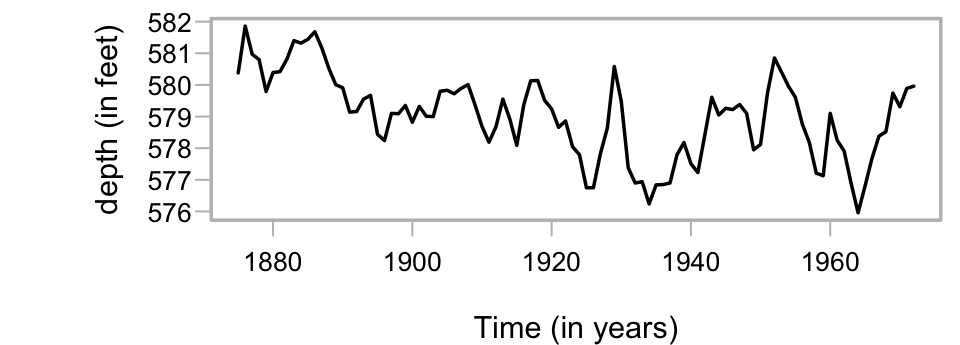
\includegraphics[width=0.8\textwidth,height=\textheight]{figs/g6_1-1.png}
\end{center}

\begin{Shaded}
\begin{Highlighting}[]
\DocumentationTok{\#\# Plot depth measurements: ts object LakeHuron (datasets)}
\FunctionTok{plot}\NormalTok{(LakeHuron, }\AttributeTok{ylab=}\StringTok{"depth (in feet)"}\NormalTok{, }\AttributeTok{xlab =} \StringTok{"Time (in years)"}\NormalTok{, }\AttributeTok{fg=}\StringTok{"gray"}\NormalTok{)}
\end{Highlighting}
\end{Shaded}

\vspace*{-4pt}

\begin{Shaded}
\begin{Highlighting}[]
\FunctionTok{lag.plot}\NormalTok{(LakeHuron, }\AttributeTok{lags=}\DecValTok{3}\NormalTok{, }\AttributeTok{do.lines=}\ConstantTok{FALSE}\NormalTok{)}
\end{Highlighting}
\end{Shaded}

\subsubsection{Subsection 6.1.3: The autocorrelation and partial
autocorrelation
function}\label{subsection-6.1.3-the-autocorrelation-and-partial-autocorrelation-function}

\begin{center}
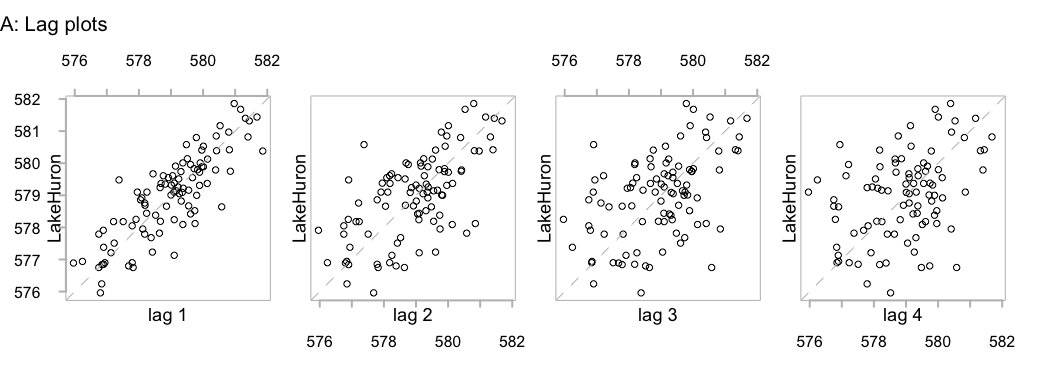
\includegraphics[width=1\textwidth,height=\textheight]{figs/g6_2A-1.png}
\end{center}

\begin{Shaded}
\begin{Highlighting}[]
\FunctionTok{par}\NormalTok{(}\AttributeTok{oma=}\FunctionTok{c}\NormalTok{(}\DecValTok{0}\NormalTok{,}\DecValTok{0}\NormalTok{,}\FloatTok{1.5}\NormalTok{,}\DecValTok{0}\NormalTok{))}
\FunctionTok{par}\NormalTok{(}\AttributeTok{pty=}\StringTok{"s"}\NormalTok{)}
\FunctionTok{lag.plot}\NormalTok{(LakeHuron, }\AttributeTok{set.lags=}\DecValTok{1}\SpecialCharTok{:}\DecValTok{4}\NormalTok{,}\AttributeTok{do.lines=}\NormalTok{F, }\AttributeTok{oma=}\FunctionTok{c}\NormalTok{(}\DecValTok{0}\NormalTok{,}\FloatTok{1.5}\NormalTok{,}\FloatTok{1.5}\NormalTok{,}\FloatTok{1.5}\NormalTok{),}
\AttributeTok{fg=}\StringTok{"gray"}\NormalTok{, }\AttributeTok{layout=}\FunctionTok{c}\NormalTok{(}\DecValTok{1}\NormalTok{,}\DecValTok{4}\NormalTok{), }\AttributeTok{cex.lab=}\FloatTok{1.15}\NormalTok{, }\AttributeTok{asp=}\DecValTok{1}\NormalTok{)}
\FunctionTok{mtext}\NormalTok{(}\AttributeTok{side=}\DecValTok{3}\NormalTok{, }\AttributeTok{line=}\FloatTok{0.5}\NormalTok{, }\StringTok{"A: Lag plots"}\NormalTok{, }\AttributeTok{adj=}\DecValTok{0}\NormalTok{, }\AttributeTok{cex=}\FloatTok{0.85}\NormalTok{, }\AttributeTok{outer=}\ConstantTok{TRUE}\NormalTok{)}
\end{Highlighting}
\end{Shaded}

\begin{center}
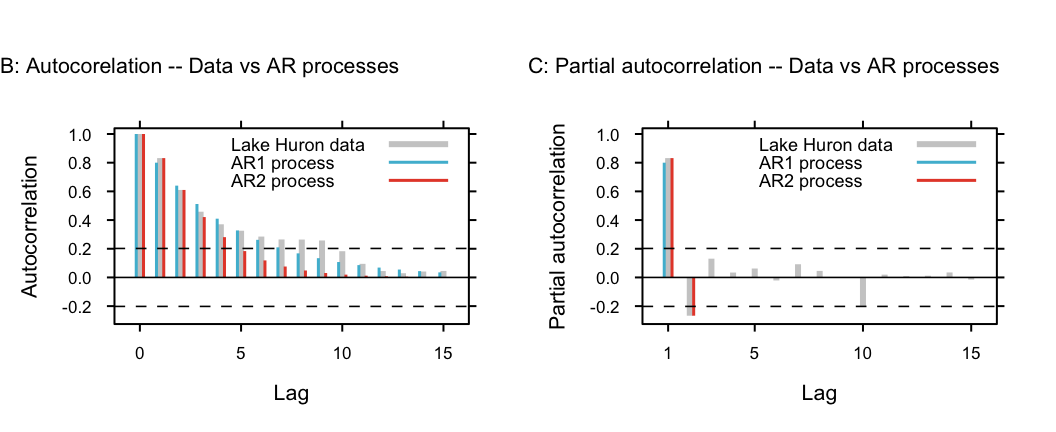
\includegraphics[width=1\textwidth,height=\textheight]{figs/g6_2B-1.png}
\end{center}

\begin{Shaded}
\begin{Highlighting}[]
\FunctionTok{library}\NormalTok{(lattice)}
\NormalTok{col3 }\OtherTok{\textless{}{-}} \FunctionTok{c}\NormalTok{(}\StringTok{"gray80"}\NormalTok{,}\FunctionTok{rev}\NormalTok{(ggsci}\SpecialCharTok{::}\FunctionTok{pal\_npg}\NormalTok{()(}\DecValTok{2}\NormalTok{)))}
\NormalTok{lag.max }\OtherTok{\textless{}{-}} \DecValTok{15}
\NormalTok{offset }\OtherTok{\textless{}{-}} \FloatTok{0.18}
\NormalTok{ci95 }\OtherTok{\textless{}{-}} \DecValTok{2}\SpecialCharTok{/}\FunctionTok{sqrt}\NormalTok{(}\FunctionTok{length}\NormalTok{(LakeHuron))}
\NormalTok{ar2 }\OtherTok{\textless{}{-}} \FunctionTok{ar}\NormalTok{(LakeHuron)}
\NormalTok{gph.key }\OtherTok{\textless{}{-}} \FunctionTok{list}\NormalTok{(}\AttributeTok{x=}\FloatTok{0.975}\NormalTok{, }\AttributeTok{y=}\FloatTok{0.965}\NormalTok{, }\AttributeTok{corner=}\FunctionTok{c}\NormalTok{(}\DecValTok{1}\NormalTok{,}\DecValTok{1}\NormalTok{), }\AttributeTok{columns=}\DecValTok{1}\NormalTok{, }\AttributeTok{cex=}\FloatTok{0.85}\NormalTok{,}
                 \AttributeTok{text=}\FunctionTok{list}\NormalTok{(}\FunctionTok{c}\NormalTok{(}\StringTok{"Lake Huron data"}\NormalTok{,}\StringTok{"AR1 process"}\NormalTok{,}\StringTok{"AR2 process"}\NormalTok{)),}
                 \AttributeTok{lines=}\FunctionTok{list}\NormalTok{(}\AttributeTok{lwd=}\FunctionTok{c}\NormalTok{(}\DecValTok{3}\NormalTok{,}\FloatTok{1.5}\NormalTok{,}\FloatTok{1.5}\NormalTok{), }\AttributeTok{col=}\NormalTok{col3,}\AttributeTok{lend=}\DecValTok{2}\NormalTok{),}
                 \AttributeTok{padding.text=}\DecValTok{1}\NormalTok{)}
\NormalTok{parsetBC }\OtherTok{\textless{}{-}} \FunctionTok{list}\NormalTok{(}\AttributeTok{fontsize=}\FunctionTok{list}\NormalTok{(}\AttributeTok{text=}\DecValTok{8}\NormalTok{, }\AttributeTok{points=}\DecValTok{5}\NormalTok{), }
                 \AttributeTok{superpose.line=}\FunctionTok{list}\NormalTok{(}\AttributeTok{col=}\NormalTok{col3, }\AttributeTok{lty=}\FunctionTok{rep}\NormalTok{(}\DecValTok{1}\NormalTok{,}\DecValTok{3}\NormalTok{),}
                 \AttributeTok{lwd=}\FunctionTok{c}\NormalTok{(}\DecValTok{3}\NormalTok{,}\FloatTok{1.5}\NormalTok{,}\FloatTok{1.5}\NormalTok{)))}
\NormalTok{parsetBC }\OtherTok{\textless{}{-}} \FunctionTok{modifyList}\NormalTok{(parsetBC,}\FunctionTok{list}\NormalTok{(}\AttributeTok{grid.pars =} \FunctionTok{list}\NormalTok{(}\AttributeTok{lineend =} \StringTok{"butt"}\NormalTok{)))}
\NormalTok{lev3 }\OtherTok{\textless{}{-}} \FunctionTok{factor}\NormalTok{(}\FunctionTok{c}\NormalTok{(}\StringTok{"acfData"}\NormalTok{,}\StringTok{"acfAR1"}\NormalTok{,}\StringTok{"acfAR2"}\NormalTok{),}
               \AttributeTok{levels=}\FunctionTok{c}\NormalTok{(}\StringTok{"acfData"}\NormalTok{,}\StringTok{"acfAR1"}\NormalTok{,}\StringTok{"acfAR2"}\NormalTok{))}
\NormalTok{acfData }\OtherTok{\textless{}{-}} \FunctionTok{acf}\NormalTok{(LakeHuron, }\AttributeTok{main=}\StringTok{""}\NormalTok{, }\AttributeTok{plot=}\ConstantTok{FALSE}\NormalTok{, }\AttributeTok{lag.max=}\NormalTok{lag.max)}\SpecialCharTok{$}\NormalTok{acf}
\NormalTok{pacfData }\OtherTok{\textless{}{-}} \FunctionTok{pacf}\NormalTok{(LakeHuron, }\AttributeTok{main=}\StringTok{""}\NormalTok{, }\AttributeTok{plot=}\ConstantTok{FALSE}\NormalTok{, }\AttributeTok{lag.max=}\NormalTok{lag.max)}\SpecialCharTok{$}\NormalTok{acf}
\NormalTok{acfAR1 }\OtherTok{\textless{}{-}} \FunctionTok{ARMAacf}\NormalTok{(}\AttributeTok{ar=}\FloatTok{0.8}\NormalTok{, }\AttributeTok{lag.max=}\NormalTok{lag.max)}
\NormalTok{acfAR2 }\OtherTok{\textless{}{-}} \FunctionTok{ARMAacf}\NormalTok{(}\AttributeTok{ar=}\NormalTok{ar2}\SpecialCharTok{$}\NormalTok{ar, }\AttributeTok{ma=}\DecValTok{0}\NormalTok{, }\AttributeTok{lag.max=}\NormalTok{lag.max)}
\NormalTok{pacfAR1 }\OtherTok{\textless{}{-}} \FunctionTok{ARMAacf}\NormalTok{(}\AttributeTok{ar=}\FloatTok{0.8}\NormalTok{, }\AttributeTok{lag.max=}\NormalTok{lag.max, }\AttributeTok{pacf=}\ConstantTok{TRUE}\NormalTok{)}
\NormalTok{pacfAR2 }\OtherTok{\textless{}{-}} \FunctionTok{ARMAacf}\NormalTok{(}\AttributeTok{ar=}\NormalTok{ar2}\SpecialCharTok{$}\NormalTok{ar, }\AttributeTok{ma=}\DecValTok{0}\NormalTok{, }\AttributeTok{lag.max=}\NormalTok{lag.max, }\AttributeTok{pacf=}\ConstantTok{TRUE}\NormalTok{)}
\NormalTok{xy }\OtherTok{\textless{}{-}} \FunctionTok{data.frame}\NormalTok{(}\AttributeTok{acf=}\FunctionTok{c}\NormalTok{(acfData,acfAR1,acfAR2),}
\AttributeTok{Lag=}\FunctionTok{c}\NormalTok{(}\FunctionTok{rep}\NormalTok{(}\DecValTok{0}\SpecialCharTok{:}\NormalTok{lag.max,}\DecValTok{3}\NormalTok{))}\SpecialCharTok{+}\FunctionTok{rep}\NormalTok{(}\FunctionTok{c}\NormalTok{(}\DecValTok{0}\NormalTok{,}\SpecialCharTok{{-}}\NormalTok{offset,offset),}
\FunctionTok{rep}\NormalTok{(lag.max}\SpecialCharTok{+}\DecValTok{1}\NormalTok{,}\DecValTok{3}\NormalTok{)),}
\AttributeTok{gp=}\FunctionTok{rep}\NormalTok{(lev3, }\FunctionTok{rep}\NormalTok{(lag.max}\SpecialCharTok{+}\DecValTok{1}\NormalTok{,}\DecValTok{3}\NormalTok{)))}
\NormalTok{gphB }\OtherTok{\textless{}{-}} \FunctionTok{xyplot}\NormalTok{(acf }\SpecialCharTok{\textasciitilde{}}\NormalTok{ Lag, }\AttributeTok{data =}\NormalTok{ xy, }\AttributeTok{groups=}\NormalTok{gp, }\AttributeTok{type=}\FunctionTok{c}\NormalTok{(}\StringTok{"h"}\NormalTok{),}
              \AttributeTok{par.strip.text =} \FunctionTok{list}\NormalTok{(}\AttributeTok{cex =} \FloatTok{0.85}\NormalTok{), }\AttributeTok{lend=}\DecValTok{2}\NormalTok{,}\AttributeTok{origin=}\DecValTok{0}\NormalTok{, }
              \AttributeTok{ylim=}\FunctionTok{c}\NormalTok{(}\SpecialCharTok{{-}}\FloatTok{0.325}\NormalTok{, }\FloatTok{1.04}\NormalTok{),}\AttributeTok{key=}\NormalTok{gph.key, }\AttributeTok{par.settings=}\NormalTok{parsetBC, }
          \AttributeTok{panel=}\ControlFlowTok{function}\NormalTok{(x,y,...)\{}
            \FunctionTok{panel.xyplot}\NormalTok{(x,y,...)}
            \FunctionTok{panel.abline}\NormalTok{(}\AttributeTok{h=}\DecValTok{0}\NormalTok{, }\AttributeTok{lwd=}\FloatTok{0.8}\NormalTok{)}
            \FunctionTok{panel.abline}\NormalTok{(}\AttributeTok{h=}\NormalTok{ci95, }\AttributeTok{lwd=}\FloatTok{0.8}\NormalTok{, }\AttributeTok{lty=}\DecValTok{2}\NormalTok{)}
            \FunctionTok{panel.abline}\NormalTok{(}\AttributeTok{h=}\SpecialCharTok{{-}}\NormalTok{ci95, }\AttributeTok{lwd=}\FloatTok{0.8}\NormalTok{, }\AttributeTok{lty=}\DecValTok{2}\NormalTok{) \} )}
\NormalTok{xyp }\OtherTok{\textless{}{-}} \FunctionTok{data.frame}\NormalTok{(}\AttributeTok{pacf=}\FunctionTok{c}\NormalTok{(pacfData,pacfAR1,pacfAR2),}
                  \AttributeTok{Lag=}\FunctionTok{c}\NormalTok{(}\FunctionTok{rep}\NormalTok{(}\DecValTok{1}\SpecialCharTok{:}\NormalTok{lag.max,}\DecValTok{3}\NormalTok{))}\SpecialCharTok{+}\FunctionTok{c}\NormalTok{(}\FunctionTok{rep}\NormalTok{(}\FunctionTok{c}\NormalTok{(}\DecValTok{0}\NormalTok{,}\SpecialCharTok{{-}}\NormalTok{offset,offset),}
                  \FunctionTok{rep}\NormalTok{(lag.max,}\DecValTok{3}\NormalTok{))), }\AttributeTok{gp=}\FunctionTok{rep}\NormalTok{(lev3, }\FunctionTok{rep}\NormalTok{(lag.max,}\DecValTok{3}\NormalTok{)))}
\NormalTok{gphC }\OtherTok{\textless{}{-}} \FunctionTok{xyplot}\NormalTok{(pacf }\SpecialCharTok{\textasciitilde{}}\NormalTok{ Lag, }\AttributeTok{data =}\NormalTok{ xyp, }\AttributeTok{groups=}\NormalTok{gp, }\AttributeTok{type=}\FunctionTok{c}\NormalTok{(}\StringTok{"h"}\NormalTok{),}
               \AttributeTok{par.strip.text =} \FunctionTok{list}\NormalTok{(}\AttributeTok{cex =} \FloatTok{0.85}\NormalTok{), }\AttributeTok{lend=}\DecValTok{2}\NormalTok{,}
               \AttributeTok{ylab =} \StringTok{"Partial correlation"}\NormalTok{, }\AttributeTok{origin=}\DecValTok{0}\NormalTok{, }\AttributeTok{ylim=}\FunctionTok{c}\NormalTok{(}\SpecialCharTok{{-}}\FloatTok{0.325}\NormalTok{, }\FloatTok{1.04}\NormalTok{),}
               \AttributeTok{key=}\NormalTok{gph.key, }\AttributeTok{par.settings=}\NormalTok{parsetBC, }
               \AttributeTok{panel=}\ControlFlowTok{function}\NormalTok{(x,y,...)\{}
                 \FunctionTok{panel.xyplot}\NormalTok{(x,y,...)}
                 \FunctionTok{panel.abline}\NormalTok{(}\AttributeTok{h=}\DecValTok{0}\NormalTok{, }\AttributeTok{lwd=}\FloatTok{0.8}\NormalTok{)}
                 \FunctionTok{panel.abline}\NormalTok{(}\AttributeTok{h=}\NormalTok{ci95, }\AttributeTok{lwd=}\FloatTok{0.8}\NormalTok{, }\AttributeTok{lty=}\DecValTok{2}\NormalTok{)}
                 \FunctionTok{panel.abline}\NormalTok{(}\AttributeTok{h=}\SpecialCharTok{{-}}\NormalTok{ci95, }\AttributeTok{lwd=}\FloatTok{0.8}\NormalTok{, }\AttributeTok{lty=}\DecValTok{2}\NormalTok{) \} )}
\FunctionTok{print}\NormalTok{(}\FunctionTok{update}\NormalTok{(gphB, }\AttributeTok{scales=}\FunctionTok{list}\NormalTok{(}\AttributeTok{alternating=}\ConstantTok{FALSE}\NormalTok{, }\AttributeTok{tck=}\FloatTok{0.5}\NormalTok{),}
             \AttributeTok{ylab =} \StringTok{"Autocorrelation"}\NormalTok{,}
             \AttributeTok{main=}\FunctionTok{list}\NormalTok{(}\StringTok{"B: Autocorelation {-}{-} Data vs AR processes"}\NormalTok{, }
                       \AttributeTok{font=}\DecValTok{1}\NormalTok{, }\AttributeTok{x=}\DecValTok{0}\NormalTok{, }\AttributeTok{y=}\FloatTok{0.25}\NormalTok{, }\AttributeTok{just=}\StringTok{"left"}\NormalTok{, }\AttributeTok{cex=}\DecValTok{1}\NormalTok{)), }
                       \AttributeTok{pos=}\FunctionTok{c}\NormalTok{(}\DecValTok{0}\NormalTok{,}\DecValTok{0}\NormalTok{,}\FloatTok{0.5}\NormalTok{,}\FloatTok{0.9}\NormalTok{))}
\FunctionTok{print}\NormalTok{(}\FunctionTok{update}\NormalTok{(gphC, }
        \AttributeTok{scales=}\FunctionTok{list}\NormalTok{(}\AttributeTok{x=}\FunctionTok{list}\NormalTok{(}\AttributeTok{at=}\FunctionTok{c}\NormalTok{(}\DecValTok{1}\NormalTok{,}\DecValTok{5}\NormalTok{,}\DecValTok{10}\NormalTok{,}\DecValTok{15}\NormalTok{)), }\AttributeTok{alternating=}\ConstantTok{FALSE}\NormalTok{, }\AttributeTok{tck=}\FloatTok{0.5}\NormalTok{),}
        \AttributeTok{ylab =} \StringTok{"Partial autocorrelation"}\NormalTok{,}
        \AttributeTok{main=}\FunctionTok{list}\NormalTok{(}\StringTok{"C: Partial autocorrelation {-}{-} Data vs AR processes"}\NormalTok{, }
                  \AttributeTok{font=}\DecValTok{1}\NormalTok{, }\AttributeTok{x=}\DecValTok{0}\NormalTok{, }\AttributeTok{y=}\FloatTok{0.25}\NormalTok{, }\AttributeTok{just=}\StringTok{"left"}\NormalTok{, }\AttributeTok{cex=}\DecValTok{1}\NormalTok{)),}
        \AttributeTok{pos=}\FunctionTok{c}\NormalTok{(}\FloatTok{0.5}\NormalTok{,}\DecValTok{0}\NormalTok{,}\DecValTok{1}\NormalTok{,}\FloatTok{0.9}\NormalTok{),}\AttributeTok{newpage=}\ConstantTok{FALSE}\NormalTok{)}
\end{Highlighting}
\end{Shaded}

\begin{Shaded}
\begin{Highlighting}[]
\FunctionTok{acf}\NormalTok{(LakeHuron)}
\DocumentationTok{\#\# pacf(LakeHuron) gives the plot of partial autocorrelations}
\end{Highlighting}
\end{Shaded}

\subsubsection{Subsection 6.1.4: Autoregressive (AR)
models}\label{subsection-6.1.4-autoregressive-ar-models}

\paragraph{\texorpdfstring{The \texttt{AR(1)}
model}{The AR(1) model}}\label{the-ar1-model}

\begin{Shaded}
\begin{Highlighting}[]
\DocumentationTok{\#\# Yule{-}Walker autocorrelation estimate}
\NormalTok{LH.yw }\OtherTok{\textless{}{-}} \FunctionTok{ar}\NormalTok{(LakeHuron, }\AttributeTok{order.max =} \DecValTok{1}\NormalTok{, }\AttributeTok{method =} \StringTok{"yw"}\NormalTok{)  }\CommentTok{\# autocorrelation estimate}
\CommentTok{\# order.max = 1 for AR(1) model}
\NormalTok{LH.yw}\SpecialCharTok{$}\NormalTok{ar                  }\CommentTok{\# autocorrelation estimate of alpha}
\end{Highlighting}
\end{Shaded}

\begin{verbatim}
[1] 0.8319112
\end{verbatim}

\begin{Shaded}
\begin{Highlighting}[]
\DocumentationTok{\#\# Maximum likelihood estimate}
\NormalTok{LH.mle }\OtherTok{\textless{}{-}} \FunctionTok{ar}\NormalTok{(LakeHuron, }\AttributeTok{order.max =} \DecValTok{1}\NormalTok{, }\AttributeTok{method =} \StringTok{"mle"}\NormalTok{)}
\NormalTok{LH.mle}\SpecialCharTok{$}\NormalTok{ar                 }\CommentTok{\# maximum likelihood estimate of alpha}
\end{Highlighting}
\end{Shaded}

\begin{verbatim}
[1] 0.837546
\end{verbatim}

\begin{Shaded}
\begin{Highlighting}[]
\NormalTok{LH.mle}\SpecialCharTok{$}\NormalTok{x.mean             }\CommentTok{\# estimated series mean}
\end{Highlighting}
\end{Shaded}

\begin{verbatim}
[1] 579.1141
\end{verbatim}

\begin{Shaded}
\begin{Highlighting}[]
\NormalTok{LH.mle}\SpecialCharTok{$}\NormalTok{var.pred           }\CommentTok{\# estimated innovation variance}
\end{Highlighting}
\end{Shaded}

\begin{verbatim}
[1] 0.5092867
\end{verbatim}

\paragraph{The general AR(p) model}\label{the-general-arp-model}

\begin{Shaded}
\begin{Highlighting}[]
\FunctionTok{ar}\NormalTok{(LakeHuron, }\AttributeTok{method=}\StringTok{"mle"}\NormalTok{)}
\end{Highlighting}
\end{Shaded}

\begin{verbatim}

Call:
ar(x = LakeHuron, method = "mle")

Coefficients:
      1        2  
 1.0437  -0.2496  

Order selected 2  sigma^2 estimated as  0.4788
\end{verbatim}

\paragraph{\textasciitilde Moving average (MA)
processes}\label{moving-average-ma-processes}

\begin{center}
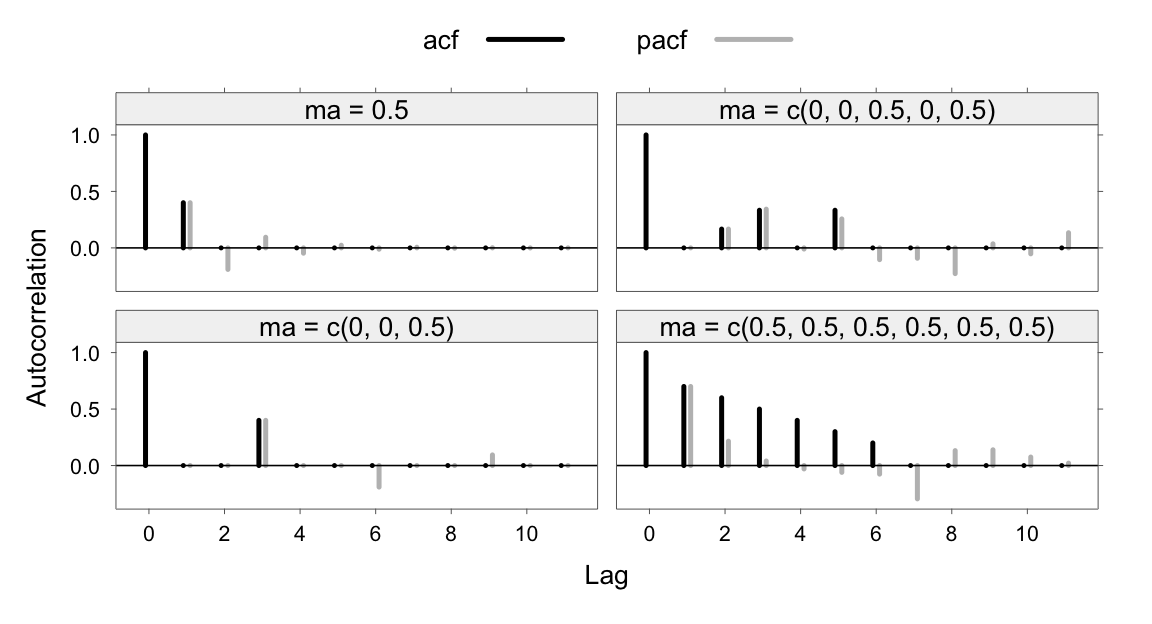
\includegraphics[width=0.8\textwidth,height=\textheight]{figs/g6_3-1.png}
\end{center}

\subsubsection{Subsection 6.1.5: \textasciitilde Autoregressive moving
average (ARMA) models --
theory}\label{subsection-6.1.5-autoregressive-moving-average-arma-models-theory}

\subsubsection{Subsection 6.1.6: Automatic model
selection?}\label{subsection-6.1.6-automatic-model-selection}

\begin{Shaded}
\begin{Highlighting}[]
\FunctionTok{library}\NormalTok{(forecast, }\AttributeTok{quietly=}\ConstantTok{TRUE}\NormalTok{)}
\NormalTok{(aaLH }\OtherTok{\textless{}{-}} \FunctionTok{auto.arima}\NormalTok{(LakeHuron, }\AttributeTok{approximation=}\NormalTok{F, }\AttributeTok{stepwise=}\NormalTok{F))}
\end{Highlighting}
\end{Shaded}

\begin{verbatim}
Series: LakeHuron 
ARIMA(2,1,1) 

Coefficients:
         ar1      ar2      ma1
      0.9712  -0.2924  -0.9108
s.e.  0.1137   0.1030   0.0712

sigma^2 = 0.5003:  log likelihood = -102.54
AIC=213.07   AICc=213.51   BIC=223.37
\end{verbatim}

\begin{Shaded}
\begin{Highlighting}[]
\DocumentationTok{\#\# Check that model removes most of the correlation structure}
\FunctionTok{acf}\NormalTok{(}\FunctionTok{resid}\NormalTok{(aaLH, }\AttributeTok{type=}\StringTok{"innovation"}\NormalTok{))   }\CommentTok{\# \textasciigrave{}type="innovation"\textasciigrave{} is the default}
\end{Highlighting}
\end{Shaded}

\begin{center}
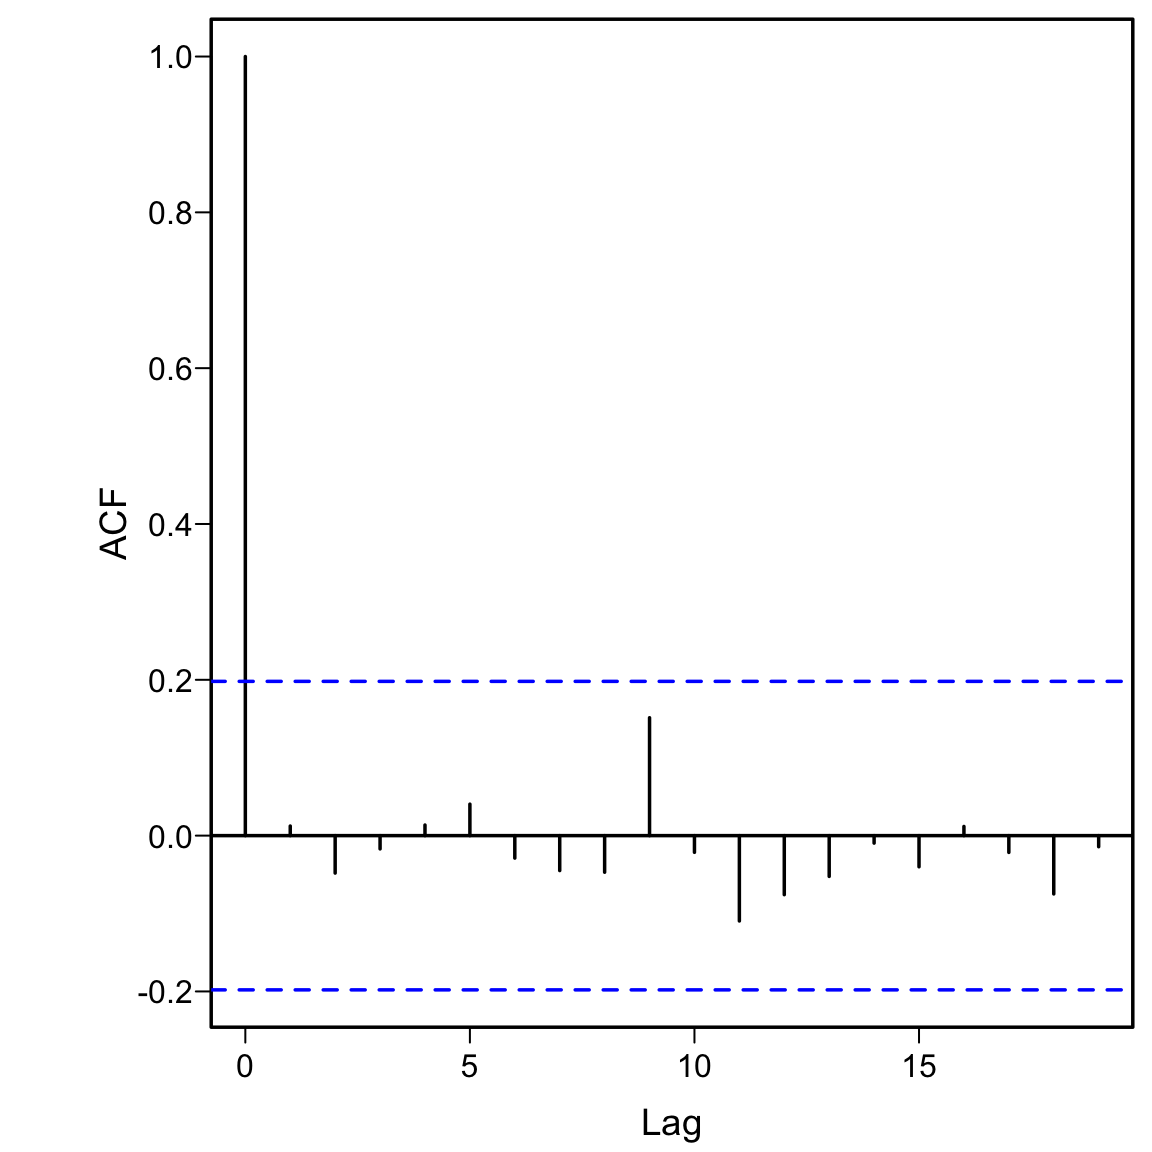
\includegraphics[width=0.8\textwidth,height=\textheight]{figs/gF1_5b-1.png}
\end{center}

\begin{Shaded}
\begin{Highlighting}[]
\FunctionTok{auto.arima}\NormalTok{(LakeHuron)}
\end{Highlighting}
\end{Shaded}

\begin{verbatim}
Series: LakeHuron 
ARIMA(0,1,0) 

sigma^2 = 0.5588:  log likelihood = -109.11
AIC=220.22   AICc=220.26   BIC=222.79
\end{verbatim}

\begin{Shaded}
\begin{Highlighting}[]
\NormalTok{(aaLH0 }\OtherTok{\textless{}{-}} \FunctionTok{auto.arima}\NormalTok{(LakeHuron, }\AttributeTok{d=}\DecValTok{0}\NormalTok{, }\AttributeTok{approximation=}\NormalTok{F, }\AttributeTok{stepwise=}\NormalTok{F))}
\end{Highlighting}
\end{Shaded}

\begin{verbatim}
Series: LakeHuron 
ARIMA(1,0,1) with non-zero mean 

Coefficients:
         ar1     ma1      mean
      0.7449  0.3206  579.0555
s.e.  0.0777  0.1135    0.3501

sigma^2 = 0.4899:  log likelihood = -103.25
AIC=214.49   AICc=214.92   BIC=224.83
\end{verbatim}

\begin{center}
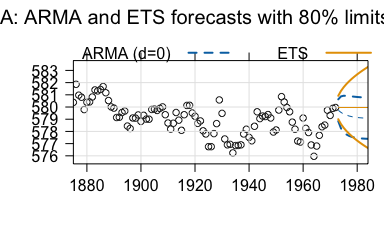
\includegraphics[width=0.48\textwidth,height=\textheight]{figs/g6_4-1.png}
\end{center}

\begin{center}
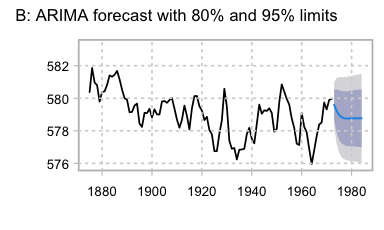
\includegraphics[width=0.48\textwidth,height=\textheight]{figs/g6_4-2.png}
\end{center}

\begin{Shaded}
\begin{Highlighting}[]
\FunctionTok{plot}\NormalTok{(}\FunctionTok{forecast}\NormalTok{(aaLH0,  }\AttributeTok{h=}\DecValTok{12}\NormalTok{))  }\DocumentationTok{\#\# \textasciigrave{}level=c(80,95)\textasciigrave{} is the default}
\NormalTok{fcETS }\OtherTok{\textless{}{-}} \FunctionTok{forecast}\NormalTok{(LakeHuron, }\AttributeTok{h=}\DecValTok{12}\NormalTok{)}
\FunctionTok{plot}\NormalTok{(fcETS)}
\FunctionTok{plot}\NormalTok{(}\FunctionTok{forecast}\NormalTok{(aaLH,  }\AttributeTok{h=}\DecValTok{12}\NormalTok{, }\AttributeTok{level=}\FunctionTok{c}\NormalTok{(}\DecValTok{80}\NormalTok{,}\DecValTok{95}\NormalTok{)))  }\CommentTok{\# Panel B; ARIMA(2,1,1)}
\end{Highlighting}
\end{Shaded}

\begin{center}
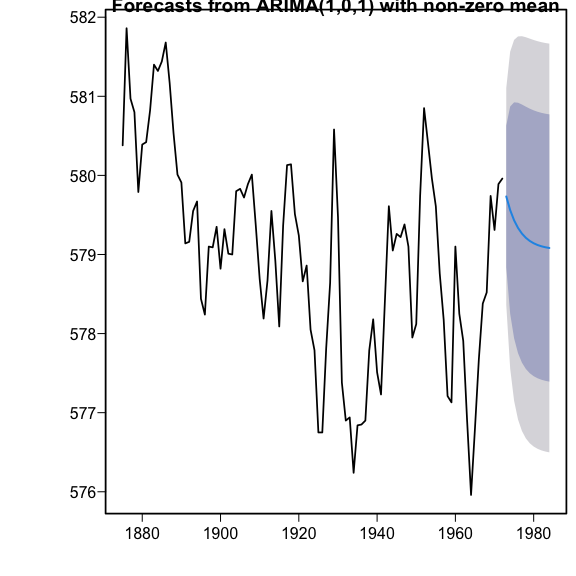
\includegraphics[width=0.8\textwidth,height=\textheight]{figs/gF1_5f-1.png}
\end{center}

\begin{center}
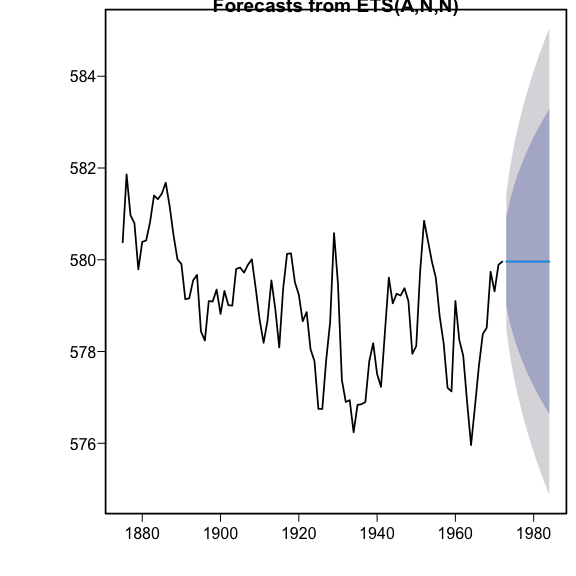
\includegraphics[width=0.8\textwidth,height=\textheight]{figs/gF1_5f-2.png}
\end{center}

\begin{center}
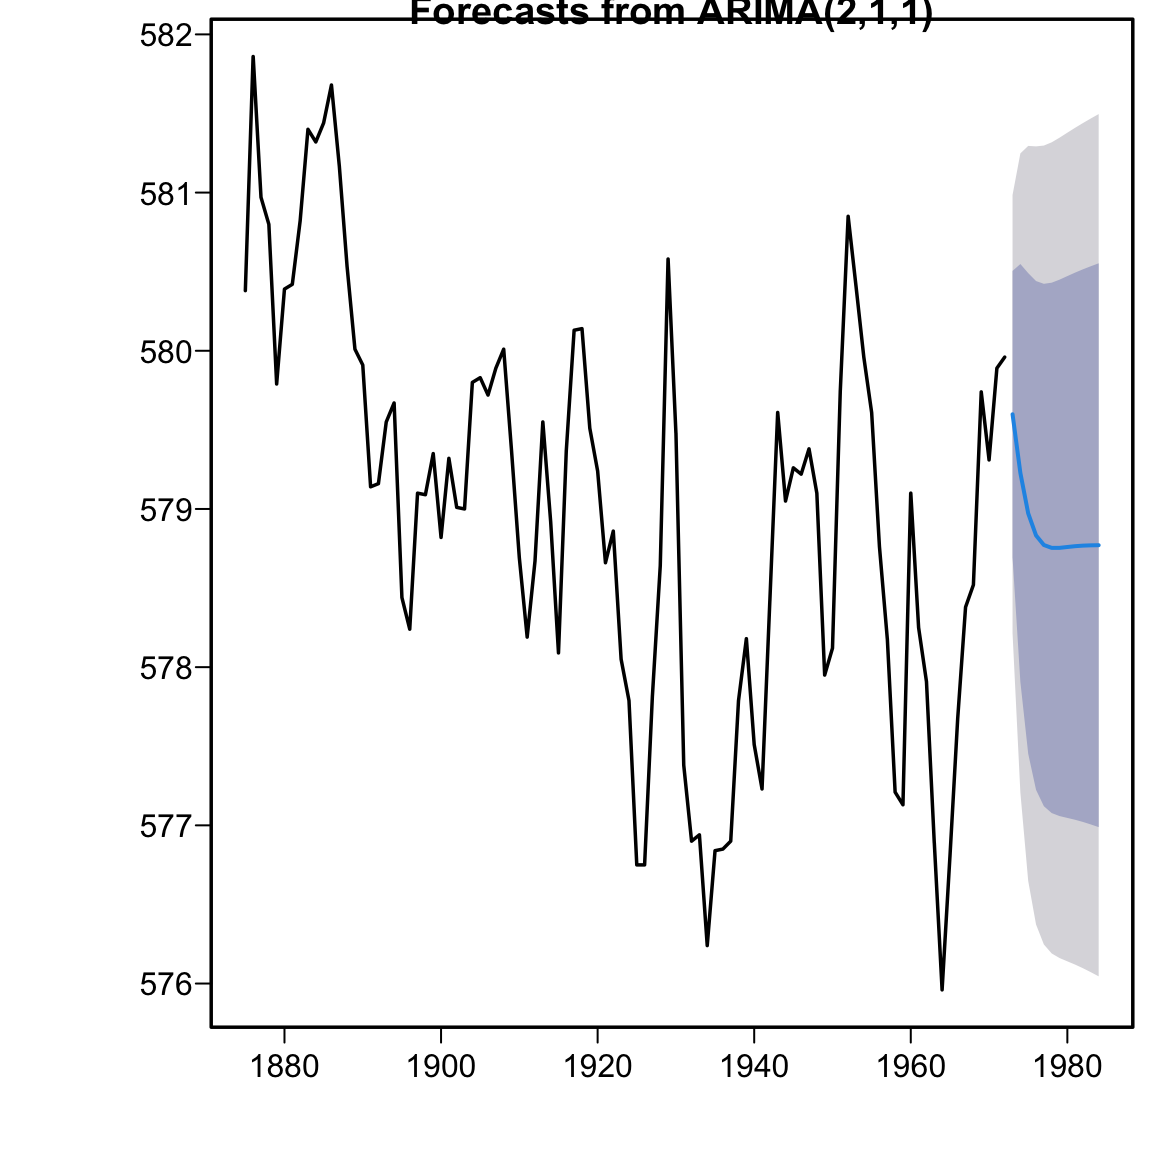
\includegraphics[width=0.8\textwidth,height=\textheight]{figs/gF1_5f-3.png}
\end{center}

\begin{Shaded}
\begin{Highlighting}[]
\FunctionTok{auto.arima}\NormalTok{(LakeHuron, }\AttributeTok{d=}\DecValTok{0}\NormalTok{, }\AttributeTok{max.Q=}\DecValTok{0}\NormalTok{, }\AttributeTok{approximation=}\NormalTok{F, }\AttributeTok{stepwise=}\NormalTok{F)}
\end{Highlighting}
\end{Shaded}

\begin{verbatim}
Series: LakeHuron 
ARIMA(1,0,1) with non-zero mean 

Coefficients:
         ar1     ma1      mean
      0.7449  0.3206  579.0555
s.e.  0.0777  0.1135    0.3501

sigma^2 = 0.4899:  log likelihood = -103.25
AIC=214.49   AICc=214.92   BIC=224.83
\end{verbatim}

\paragraph{Use of simulation as a
check}\label{use-of-simulation-as-a-check}

\begin{center}
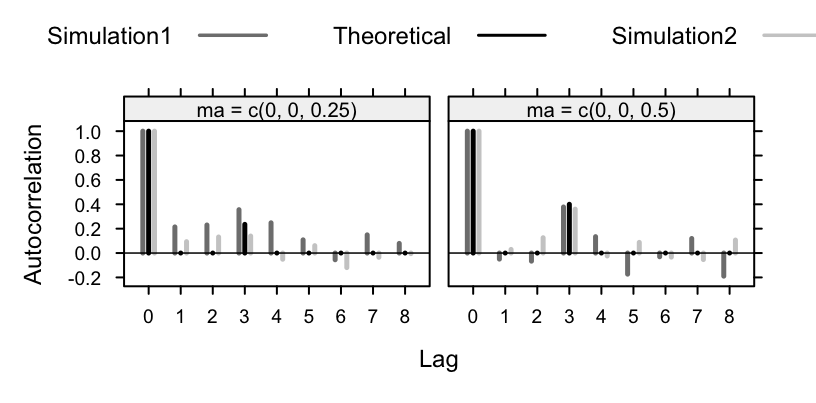
\includegraphics[width=1\textwidth,height=\textheight]{figs/g6_5-1.png}
\end{center}

\begin{Shaded}
\begin{Highlighting}[]
\NormalTok{oldpar }\OtherTok{\textless{}{-}} \FunctionTok{par}\NormalTok{(}\AttributeTok{mfrow=}\FunctionTok{c}\NormalTok{(}\DecValTok{2}\NormalTok{,}\DecValTok{2}\NormalTok{), }\AttributeTok{mar=}\FunctionTok{c}\NormalTok{(}\FloatTok{3.1}\NormalTok{,}\FloatTok{4.6}\NormalTok{,}\FloatTok{2.6}\NormalTok{, }\FloatTok{1.1}\NormalTok{))}
\ControlFlowTok{for}\NormalTok{(i }\ControlFlowTok{in} \DecValTok{1}\SpecialCharTok{:}\DecValTok{2}\NormalTok{)\{}
\NormalTok{  simts }\OtherTok{\textless{}{-}} \FunctionTok{arima.sim}\NormalTok{(}\AttributeTok{model=}\FunctionTok{list}\NormalTok{(}\AttributeTok{order=}\FunctionTok{c}\NormalTok{(}\DecValTok{0}\NormalTok{,}\DecValTok{0}\NormalTok{,}\DecValTok{3}\NormalTok{), }\AttributeTok{ma=}\FunctionTok{c}\NormalTok{(}\DecValTok{0}\NormalTok{,}\DecValTok{0}\NormalTok{,}\FloatTok{0.25}\SpecialCharTok{*}\NormalTok{i)), }\AttributeTok{n=}\DecValTok{98}\NormalTok{)}
  \FunctionTok{acf}\NormalTok{(simts, }\AttributeTok{main=}\StringTok{""}\NormalTok{, }\AttributeTok{xlab=}\StringTok{""}\NormalTok{)}
  \FunctionTok{mtext}\NormalTok{(}\AttributeTok{side=}\DecValTok{3}\NormalTok{, }\AttributeTok{line=}\FloatTok{0.5}\NormalTok{, }\FunctionTok{paste}\NormalTok{(}\StringTok{"ma3 ="}\NormalTok{, }\FloatTok{0.25}\SpecialCharTok{*}\NormalTok{i), }\AttributeTok{adj=}\DecValTok{0}\NormalTok{)}
\NormalTok{\}}
\FunctionTok{par}\NormalTok{(oldpar)}
\end{Highlighting}
\end{Shaded}

\begin{center}
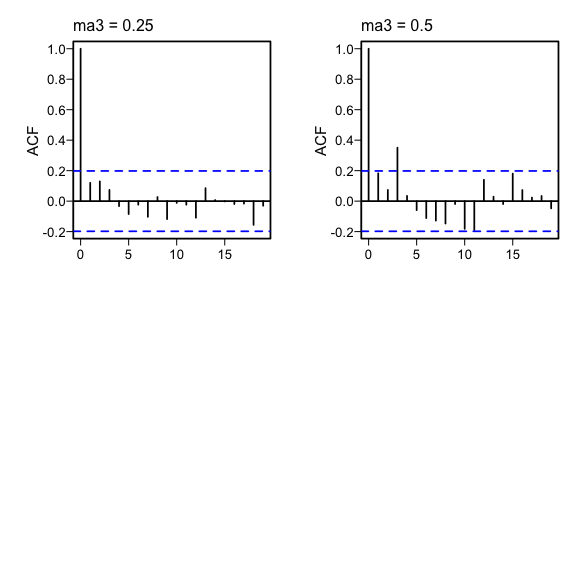
\includegraphics[width=0.8\textwidth,height=\textheight]{figs/gF1_6c-1.png}
\end{center}

\begin{Shaded}
\begin{Highlighting}[]
\FunctionTok{set.seed}\NormalTok{(}\DecValTok{29}\NormalTok{)         }\CommentTok{\# Ensure that results are reproducible}
\NormalTok{estMAord }\OtherTok{\textless{}{-}} \FunctionTok{matrix}\NormalTok{(}\DecValTok{0}\NormalTok{, }\AttributeTok{nrow=}\DecValTok{4}\NormalTok{, }\AttributeTok{ncol=}\DecValTok{20}\NormalTok{)}
\ControlFlowTok{for}\NormalTok{(i }\ControlFlowTok{in} \DecValTok{1}\SpecialCharTok{:}\DecValTok{4}\NormalTok{)\{}
  \ControlFlowTok{for}\NormalTok{(j }\ControlFlowTok{in} \DecValTok{1}\SpecialCharTok{:}\DecValTok{20}\NormalTok{)\{}
\NormalTok{    simts }\OtherTok{\textless{}{-}} \FunctionTok{arima.sim}\NormalTok{(}\AttributeTok{n=}\DecValTok{98}\NormalTok{, }\AttributeTok{model=}\FunctionTok{list}\NormalTok{(}\AttributeTok{ma=}\FunctionTok{c}\NormalTok{(}\DecValTok{0}\NormalTok{,}\DecValTok{0}\NormalTok{,}\FloatTok{0.125}\SpecialCharTok{*}\NormalTok{i)))}
\NormalTok{    estMAord[i,j] }\OtherTok{\textless{}{-}} \FunctionTok{auto.arima}\NormalTok{(simts, }\AttributeTok{start.q=}\DecValTok{3}\NormalTok{)}\SpecialCharTok{$}\NormalTok{arma[}\DecValTok{2}\NormalTok{] \}}
\NormalTok{\}}
\NormalTok{detectedAs }\OtherTok{\textless{}{-}} \FunctionTok{table}\NormalTok{(}\FunctionTok{row}\NormalTok{(estMAord), estMAord)}
\FunctionTok{dimnames}\NormalTok{(detectedAs) }\OtherTok{\textless{}{-}} \FunctionTok{list}\NormalTok{(}\AttributeTok{ma3=}\FunctionTok{paste}\NormalTok{(}\FloatTok{0.125}\SpecialCharTok{*}\NormalTok{(}\DecValTok{1}\SpecialCharTok{:}\DecValTok{4}\NormalTok{)),}
\AttributeTok{Order=}\FunctionTok{paste}\NormalTok{(}\DecValTok{0}\SpecialCharTok{:}\NormalTok{(}\FunctionTok{dim}\NormalTok{(detectedAs)[}\DecValTok{2}\NormalTok{]}\SpecialCharTok{{-}}\DecValTok{1}\NormalTok{)))}
\end{Highlighting}
\end{Shaded}

\begin{Shaded}
\begin{Highlighting}[]
\FunctionTok{print}\NormalTok{(detectedAs)}
\end{Highlighting}
\end{Shaded}

\begin{verbatim}
       Order
ma3      0  1  2  3  4
  0.125 18  2  0  0  0
  0.25  11  3  0  6  0
  0.375  7  2  2  7  2
  0.5    1  1  0 13  5
\end{verbatim}

\subsubsection{Subsection 6.1.7: Seasonal
effects}\label{subsection-6.1.7-seasonal-effects}

\begin{center}
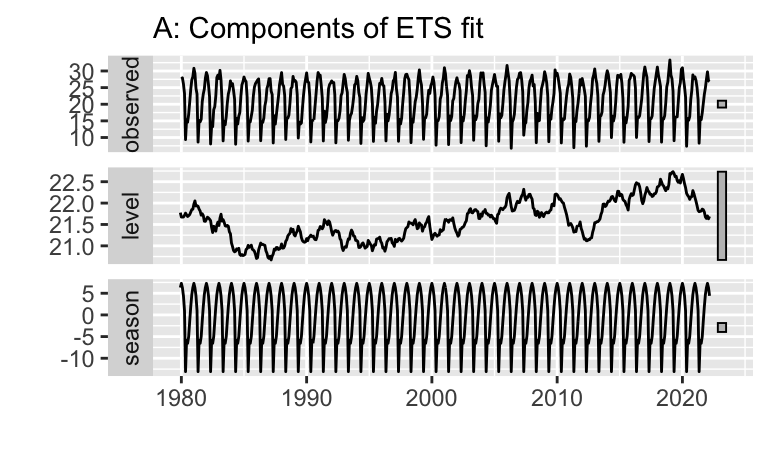
\includegraphics[width=0.48\textwidth,height=\textheight]{figs/g6_6-1.png}
\end{center}

\begin{center}
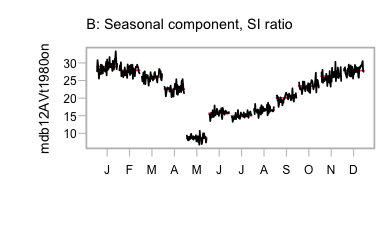
\includegraphics[width=0.48\textwidth,height=\textheight]{figs/g6_6-2.png}
\end{center}

\begin{Shaded}
\begin{Highlighting}[]
\FunctionTok{suppressPackageStartupMessages}\NormalTok{(}\FunctionTok{library}\NormalTok{(ggplot2))}
\NormalTok{mdb12AVt1980on }\OtherTok{\textless{}{-}} \FunctionTok{window}\NormalTok{(DAAG}\SpecialCharTok{::}\NormalTok{mdbAVtJtoD, }\FunctionTok{c}\NormalTok{(}\DecValTok{1980}\NormalTok{,}\DecValTok{1}\NormalTok{))}
\NormalTok{AVt.ets }\OtherTok{\textless{}{-}} \FunctionTok{ets}\NormalTok{(mdb12AVt1980on)}
\FunctionTok{autoplot}\NormalTok{(AVt.ets, }\AttributeTok{main=}\StringTok{""}\NormalTok{, }\AttributeTok{fg=}\StringTok{"gray"}\NormalTok{) }\SpecialCharTok{+} 
\NormalTok{  ggplot2}\SpecialCharTok{::}\FunctionTok{ggtitle}\NormalTok{(}\StringTok{"A: Components of ETS fit"}\NormalTok{) }\SpecialCharTok{+}
    \FunctionTok{theme}\NormalTok{(}\AttributeTok{plot.title =} \FunctionTok{element\_text}\NormalTok{(}\AttributeTok{hjust=}\DecValTok{0}\NormalTok{, }\AttributeTok{vjust=}\FloatTok{0.5}\NormalTok{, }\AttributeTok{size=}\DecValTok{11}\NormalTok{))}
\FunctionTok{monthplot}\NormalTok{(mdb12AVt1980on, }\AttributeTok{col.base=}\DecValTok{2}\NormalTok{,  }\AttributeTok{fg=}\StringTok{"gray"}\NormalTok{)}
\FunctionTok{title}\NormalTok{(}\StringTok{"B: Seasonal component, SI ratio"}\NormalTok{, }
      \AttributeTok{font.main=}\DecValTok{1}\NormalTok{, }\AttributeTok{line=}\DecValTok{1}\NormalTok{, }\AttributeTok{adj=}\DecValTok{0}\NormalTok{, }\AttributeTok{cex=}\FloatTok{1.25}\NormalTok{)}
\end{Highlighting}
\end{Shaded}

\begin{center}
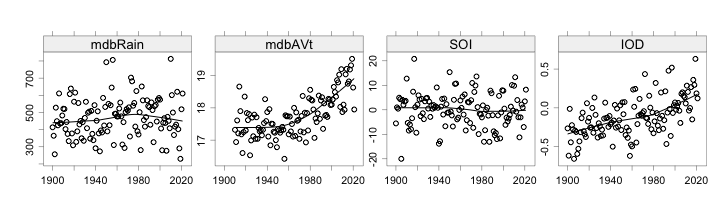
\includegraphics[width=1\textwidth,height=\textheight]{figs/g6_7-1.png}
\end{center}

\begin{Shaded}
\begin{Highlighting}[]
\NormalTok{bomreg }\OtherTok{\textless{}{-}}\NormalTok{ DAAG}\SpecialCharTok{::}\NormalTok{bomregions2021}
\DocumentationTok{\#\# Plot time series mdbRain, SOI, and IOD: ts object bomregions2021 (DAAG)}
\NormalTok{gph }\OtherTok{\textless{}{-}} \FunctionTok{xyplot}\NormalTok{(}\FunctionTok{ts}\NormalTok{(bomreg[, }\FunctionTok{c}\NormalTok{(}\StringTok{"mdbRain"}\NormalTok{, }\StringTok{"mdbAVt"}\NormalTok{, }\StringTok{"SOI"}\NormalTok{, }\StringTok{"IOD"}\NormalTok{)], }\AttributeTok{start=}\DecValTok{1900}\NormalTok{), }
              \AttributeTok{xlab=}\StringTok{""}\NormalTok{, }\AttributeTok{type=}\FunctionTok{c}\NormalTok{(}\StringTok{\textquotesingle{}p\textquotesingle{}}\NormalTok{,}\StringTok{\textquotesingle{}smooth\textquotesingle{}}\NormalTok{), }\AttributeTok{scales=}\FunctionTok{list}\NormalTok{(}\AttributeTok{alternating=}\FunctionTok{rep}\NormalTok{(}\DecValTok{1}\NormalTok{,}\DecValTok{3}\NormalTok{)))}
\FunctionTok{update}\NormalTok{(gph, }\AttributeTok{layout=}\FunctionTok{c}\NormalTok{(}\DecValTok{4}\NormalTok{,}\DecValTok{1}\NormalTok{), }\AttributeTok{par.settings=}\NormalTok{DAAG}\SpecialCharTok{::}\FunctionTok{DAAGtheme}\NormalTok{(}\AttributeTok{color=}\NormalTok{F))}
\end{Highlighting}
\end{Shaded}

\begin{Shaded}
\begin{Highlighting}[]
\FunctionTok{suppressPackageStartupMessages}\NormalTok{(}\FunctionTok{library}\NormalTok{(mgcv))}
\NormalTok{bomreg }\OtherTok{\textless{}{-}} \FunctionTok{within}\NormalTok{(DAAG}\SpecialCharTok{::}\NormalTok{bomregions2021, mdbrtRain }\OtherTok{\textless{}{-}}\NormalTok{ mdbRain}\SpecialCharTok{\^{}}\FloatTok{0.5}\NormalTok{)}
\DocumentationTok{\#\# Check first for a sequential correlation structure, after}
\DocumentationTok{\#\# fitting smooth terms s(CO2), s(SOI), and s(IOD)}
\FunctionTok{library}\NormalTok{(mgcv)}
\NormalTok{mdbrtRain.gam }\OtherTok{\textless{}{-}} \FunctionTok{gam}\NormalTok{(mdbrtRain}\SpecialCharTok{\textasciitilde{}}\FunctionTok{s}\NormalTok{(CO2) }\SpecialCharTok{+} \FunctionTok{s}\NormalTok{(SOI) }\SpecialCharTok{+} \FunctionTok{s}\NormalTok{(IOD), }\AttributeTok{data=}\NormalTok{bomreg)}
\FunctionTok{auto.arima}\NormalTok{(}\FunctionTok{resid}\NormalTok{(mdbrtRain.gam))}
\end{Highlighting}
\end{Shaded}

\begin{verbatim}
Series: resid(mdbrtRain.gam) 
ARIMA(0,0,0) with zero mean 

sigma^2 = 4.424:  log likelihood = -263.82
AIC=529.64   AICc=529.67   BIC=532.44
\end{verbatim}

\begin{center}
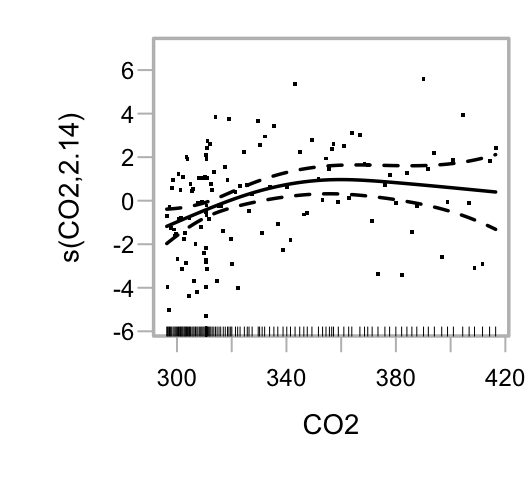
\includegraphics[width=0.32\textwidth,height=\textheight]{figs/g6_8-1.png}
\end{center}

\begin{center}
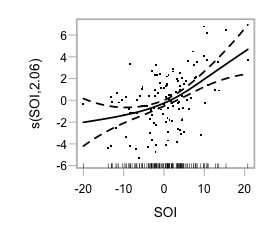
\includegraphics[width=0.32\textwidth,height=\textheight]{figs/g6_8-2.png}
\end{center}

\begin{center}
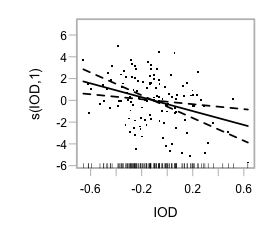
\includegraphics[width=0.32\textwidth,height=\textheight]{figs/g6_8-3.png}
\end{center}

\begin{Shaded}
\begin{Highlighting}[]
\FunctionTok{plot}\NormalTok{(mdbrtRain.gam, }\AttributeTok{residuals=}\NormalTok{T, }\AttributeTok{cex=}\DecValTok{2}\NormalTok{, }\AttributeTok{fg=}\StringTok{"gray"}\NormalTok{)}
\DocumentationTok{\#\# Do also \textasciigrave{}gam.check(mdbrtRain.gam)\textasciigrave{} (Output looks fine)}
\end{Highlighting}
\end{Shaded}

\begin{Shaded}
\begin{Highlighting}[]
\FunctionTok{anova}\NormalTok{(mdbrtRain.gam)}
\end{Highlighting}
\end{Shaded}

\begin{verbatim}

Family: gaussian 
Link function: identity 

Formula:
mdbrtRain ~ s(CO2) + s(SOI) + s(IOD)

Approximate significance of smooth terms:
         edf Ref.df      F  p-value
s(CO2) 2.144  2.673  4.345  0.01090
s(SOI) 2.058  2.637 12.581 2.72e-06
s(IOD) 1.000  1.000  9.696  0.00233
\end{verbatim}

\begin{Shaded}
\begin{Highlighting}[]
\FunctionTok{Box.test}\NormalTok{(}\FunctionTok{resid}\NormalTok{(mdbrtRain.gam), }\AttributeTok{lag=}\DecValTok{10}\NormalTok{, }\AttributeTok{type=}\StringTok{"Ljung"}\NormalTok{)}
\end{Highlighting}
\end{Shaded}

\begin{verbatim}

    Box-Ljung test

data:  resid(mdbrtRain.gam)
X-squared = 11.935, df = 10, p-value = 0.2894
\end{verbatim}

\begin{Shaded}
\begin{Highlighting}[]
\DocumentationTok{\#\# Examine normality of estimates of "residuals" }
\FunctionTok{qqnorm}\NormalTok{(}\FunctionTok{resid}\NormalTok{(mdbrtRain.gam))}
\end{Highlighting}
\end{Shaded}

\paragraph{The mdbAVt series}\label{the-mdbavt-series}

\begin{Shaded}
\begin{Highlighting}[]
\NormalTok{mdbAVt.gam }\OtherTok{\textless{}{-}} \FunctionTok{gam}\NormalTok{(mdbAVt }\SpecialCharTok{\textasciitilde{}} \FunctionTok{s}\NormalTok{(CO2)}\SpecialCharTok{+}\FunctionTok{s}\NormalTok{(SOI)}\SpecialCharTok{+}\FunctionTok{s}\NormalTok{(IOD), }\AttributeTok{data=}\NormalTok{bomreg)}
\FunctionTok{auto.arima}\NormalTok{(}\FunctionTok{resid}\NormalTok{(mdbAVt.gam))}
\end{Highlighting}
\end{Shaded}

\begin{verbatim}
Series: resid(mdbAVt.gam) 
ARIMA(0,0,0) with zero mean 

sigma^2 = 0.1689:  log likelihood = -59.33
AIC=120.67   AICc=120.7   BIC=123.39
\end{verbatim}

\begin{Shaded}
\begin{Highlighting}[]
\FunctionTok{anova}\NormalTok{(mdbAVt.gam)}
\end{Highlighting}
\end{Shaded}

\begin{verbatim}

Family: gaussian 
Link function: identity 

Formula:
mdbAVt ~ s(CO2) + s(SOI) + s(IOD)

Approximate significance of smooth terms:
         edf Ref.df      F p-value
s(CO2) 1.855  2.312 41.842 < 2e-16
s(SOI) 1.000  1.000 10.688 0.00145
s(IOD) 1.000  1.000  0.005 0.94403
\end{verbatim}

\begin{Shaded}
\begin{Highlighting}[]
\NormalTok{mdbAVt1.gam }\OtherTok{\textless{}{-}} \FunctionTok{gam}\NormalTok{(mdbAVt }\SpecialCharTok{\textasciitilde{}} \FunctionTok{s}\NormalTok{(CO2)}\SpecialCharTok{+}\FunctionTok{s}\NormalTok{(SOI), }\AttributeTok{data=}\NormalTok{bomreg)}
\end{Highlighting}
\end{Shaded}

\begin{Shaded}
\begin{Highlighting}[]
\FunctionTok{plot}\NormalTok{(mdbAVt1.gam, }\AttributeTok{residuals=}\ConstantTok{TRUE}\NormalTok{)}
\end{Highlighting}
\end{Shaded}

\begin{center}
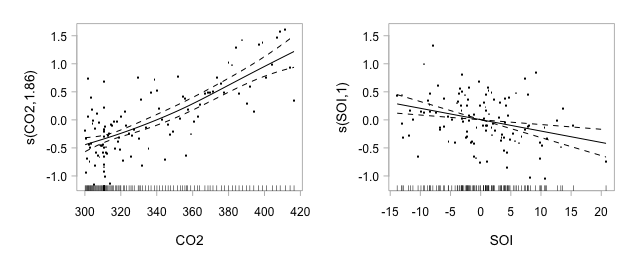
\includegraphics[width=1\textwidth,height=\textheight]{figs/g6_9-1.png}
\end{center}

\begin{center}
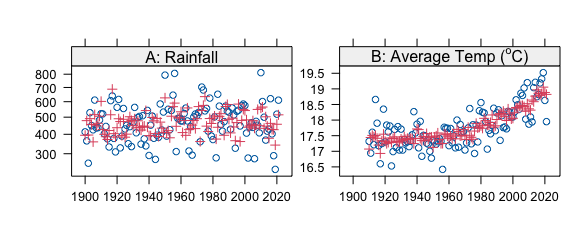
\includegraphics[width=1\textwidth,height=\textheight]{figs/g6_10-1.png}
\end{center}

\begin{Shaded}
\begin{Highlighting}[]
\NormalTok{faclevs }\OtherTok{\textless{}{-}} \FunctionTok{c}\NormalTok{(}\StringTok{"A: Rainfall"}\NormalTok{, }\FunctionTok{expression}\NormalTok{(}\StringTok{"B: Average Temp ("}\SpecialCharTok{\^{}}\NormalTok{o}\SpecialCharTok{*}\StringTok{"C)"}\NormalTok{))}
\NormalTok{fitrain }\OtherTok{\textless{}{-}} \FunctionTok{fitted}\NormalTok{(mdbrtRain.gam) }
\NormalTok{fitAVt }\OtherTok{\textless{}{-}} \FunctionTok{c}\NormalTok{(}\FunctionTok{rep}\NormalTok{(}\ConstantTok{NA}\NormalTok{,}\DecValTok{10}\NormalTok{), }\FunctionTok{fitted}\NormalTok{(mdbAVt1.gam))}
\NormalTok{gph }\OtherTok{\textless{}{-}} \FunctionTok{xyplot}\NormalTok{(mdbrtRain}\SpecialCharTok{+}\NormalTok{mdbAVt}\SpecialCharTok{\textasciitilde{}}\NormalTok{Year,}\AttributeTok{data=}\NormalTok{bomreg, }\AttributeTok{outer=}\NormalTok{T, }\AttributeTok{xlab=}\StringTok{""}\NormalTok{, }\AttributeTok{ylab=}\StringTok{""}\NormalTok{,}
  \AttributeTok{scales=}\FunctionTok{list}\NormalTok{(}\AttributeTok{y=}\FunctionTok{list}\NormalTok{(}\AttributeTok{relation=}\StringTok{\textquotesingle{}free\textquotesingle{}}\NormalTok{, }
              \AttributeTok{at=}\FunctionTok{list}\NormalTok{(}\FunctionTok{sqrt}\NormalTok{((}\DecValTok{3}\SpecialCharTok{:}\DecValTok{8}\NormalTok{)}\SpecialCharTok{*}\DecValTok{100}\NormalTok{),(}\DecValTok{33}\SpecialCharTok{:}\DecValTok{39}\NormalTok{)}\SpecialCharTok{/}\DecValTok{2}\NormalTok{), }
              \AttributeTok{labels=}\FunctionTok{list}\NormalTok{((}\DecValTok{3}\SpecialCharTok{:}\DecValTok{8}\NormalTok{)}\SpecialCharTok{*}\DecValTok{100}\NormalTok{,(}\DecValTok{33}\SpecialCharTok{:}\DecValTok{39}\NormalTok{)}\SpecialCharTok{/}\DecValTok{2}\NormalTok{)), }\AttributeTok{x=}\FunctionTok{list}\NormalTok{(}\AttributeTok{alternating=}\FunctionTok{rep}\NormalTok{(}\DecValTok{1}\NormalTok{,}\DecValTok{2}\NormalTok{))),}
  \AttributeTok{strip=}\FunctionTok{strip.custom}\NormalTok{(}\AttributeTok{factor.levels=}\NormalTok{faclevs))}
\NormalTok{gph }\SpecialCharTok{+}\NormalTok{ latticeExtra}\SpecialCharTok{::}\FunctionTok{as.layer}\NormalTok{(}\FunctionTok{xyplot}\NormalTok{(fitrain}\SpecialCharTok{+}\NormalTok{fitAVt}\SpecialCharTok{\textasciitilde{}}\NormalTok{Year, }\AttributeTok{outer=}\NormalTok{T,}
                                    \AttributeTok{scales=}\FunctionTok{list}\NormalTok{(}\AttributeTok{y=}\FunctionTok{list}\NormalTok{(}\AttributeTok{relation=}\StringTok{\textquotesingle{}free\textquotesingle{}}\NormalTok{)), }
                                    \AttributeTok{data=}\NormalTok{bomreg, }\AttributeTok{pch=}\DecValTok{3}\NormalTok{, }\AttributeTok{col=}\DecValTok{2}\NormalTok{))}
\end{Highlighting}
\end{Shaded}

\begin{Shaded}
\begin{Highlighting}[]
\DocumentationTok{\#\# Use \textasciigrave{}auto.arima()\textasciigrave{} to choose the ARIMA order:}
\NormalTok{aaFitCO2 }\OtherTok{\textless{}{-}} \FunctionTok{with}\NormalTok{(bomreg[}\SpecialCharTok{{-}}\NormalTok{(}\DecValTok{1}\SpecialCharTok{:}\DecValTok{10}\NormalTok{),], }\FunctionTok{auto.arima}\NormalTok{(mdbAVt, }\AttributeTok{xreg=}\FunctionTok{cbind}\NormalTok{(CO2,SOI)))}
\DocumentationTok{\#\# Try including a degree 2 polynomial term}
\NormalTok{aaFitpol2CO2 }\OtherTok{\textless{}{-}} \FunctionTok{with}\NormalTok{(bomreg[}\SpecialCharTok{{-}}\NormalTok{(}\DecValTok{1}\SpecialCharTok{:}\DecValTok{10}\NormalTok{),], }
                     \FunctionTok{auto.arima}\NormalTok{(mdbAVt, }\AttributeTok{xreg=}\FunctionTok{cbind}\NormalTok{(}\FunctionTok{poly}\NormalTok{(CO2,}\DecValTok{2}\NormalTok{),SOI)))}
\FunctionTok{cbind}\NormalTok{(}\FunctionTok{AIC}\NormalTok{(aaFitCO2, aaFitpol2CO2), }\AttributeTok{BIC=}\FunctionTok{BIC}\NormalTok{(aaFitCO2, aaFitpol2CO2))}
\end{Highlighting}
\end{Shaded}

\begin{verbatim}
             df      AIC BIC.df  BIC.BIC
aaFitCO2      7 125.3765      7 144.4060
aaFitpol2CO2  5 129.0109      5 142.6033
\end{verbatim}

\subsubsection{\texorpdfstring{Subsection 6.1.8: The \texttt{gamm()}
function, with a correlated errors
model}{Subsection 6.1.8: The gamm() function, with a correlated errors model}}\label{subsection-6.1.8-the-gamm-function-with-a-correlated-errors-model}

\begin{Shaded}
\begin{Highlighting}[]
\NormalTok{SOI.gam }\OtherTok{\textless{}{-}} \FunctionTok{gam}\NormalTok{(SOI}\SpecialCharTok{\textasciitilde{}}\FunctionTok{s}\NormalTok{(Year), }\AttributeTok{data=}\NormalTok{bomreg)}
\FunctionTok{auto.arima}\NormalTok{(}\FunctionTok{resid}\NormalTok{(SOI.gam))             }\CommentTok{\# sigma\^{}2 = 43.4}
\end{Highlighting}
\end{Shaded}

\begin{verbatim}
Series: resid(SOI.gam) 
ARIMA(0,0,2) with zero mean 

Coefficients:
         ma1      ma2
      0.2070  -0.1557
s.e.  0.0943   0.1008

sigma^2 = 43.43:  log likelihood = -402.2
AIC=810.41   AICc=810.61   BIC=818.82
\end{verbatim}

\begin{Shaded}
\begin{Highlighting}[]
\DocumentationTok{\#\# The following breaks the model into two parts {-}{-} gam and lme}
\NormalTok{SOI.gamm }\OtherTok{\textless{}{-}} \FunctionTok{gamm}\NormalTok{(SOI}\SpecialCharTok{\textasciitilde{}}\FunctionTok{s}\NormalTok{(Year), }\AttributeTok{data=}\NormalTok{bomreg)       }
\NormalTok{res }\OtherTok{\textless{}{-}} \FunctionTok{resid}\NormalTok{(SOI.gamm}\SpecialCharTok{$}\NormalTok{lme, }\AttributeTok{type=}\StringTok{"normalized"}\NormalTok{)}
\FunctionTok{auto.arima}\NormalTok{(res)                        }\CommentTok{\# sigma\^{}2 = 0.945}
\end{Highlighting}
\end{Shaded}

\begin{verbatim}
Series: res 
ARIMA(0,0,2) with zero mean 

Coefficients:
         ma1      ma2
      0.2070  -0.1557
s.e.  0.0943   0.1008

sigma^2 = 0.9446:  log likelihood = -168.68
AIC=343.37   AICc=343.57   BIC=351.78
\end{verbatim}

\begin{Shaded}
\begin{Highlighting}[]
\DocumentationTok{\#\# Extract scale estimate for \textasciigrave{}gam\textasciigrave{} component of SOI.gamm}
\FunctionTok{summary}\NormalTok{(SOI.gamm}\SpecialCharTok{$}\NormalTok{gam)[[}\StringTok{\textquotesingle{}scale\textquotesingle{}}\NormalTok{]]       }\CommentTok{\# 45.98}
\end{Highlighting}
\end{Shaded}

\begin{verbatim}
[1] 45.98091
\end{verbatim}

\begin{Shaded}
\begin{Highlighting}[]
  \CommentTok{\# Note that 45.98 x .945 \textasciitilde{}= 43.4}
\end{Highlighting}
\end{Shaded}

\begin{Shaded}
\begin{Highlighting}[]
\NormalTok{SOIma2.gamm }\OtherTok{\textless{}{-}} \FunctionTok{gamm}\NormalTok{(SOI}\SpecialCharTok{\textasciitilde{}}\FunctionTok{s}\NormalTok{(Year), }\AttributeTok{data=}\NormalTok{bomreg, }\AttributeTok{correlation=}\FunctionTok{corARMA}\NormalTok{(}\AttributeTok{q=}\DecValTok{2}\NormalTok{))}
\FunctionTok{coef}\NormalTok{(SOIma2.gamm}\SpecialCharTok{$}\NormalTok{lme}\SpecialCharTok{$}\NormalTok{modelStruct}\SpecialCharTok{$}\NormalTok{corStruct, }\AttributeTok{unconstrained =} \ConstantTok{FALSE}\NormalTok{)  }\CommentTok{\# MA2 ests}
\end{Highlighting}
\end{Shaded}

\begin{verbatim}
    Theta1     Theta2 
 0.2070115 -0.1557351 
\end{verbatim}

\begin{Shaded}
\begin{Highlighting}[]
\NormalTok{SOIar2.gamm }\OtherTok{\textless{}{-}} \FunctionTok{gamm}\NormalTok{(SOI}\SpecialCharTok{\textasciitilde{}}\FunctionTok{s}\NormalTok{(Year), }\AttributeTok{data=}\NormalTok{bomreg, }\AttributeTok{correlation=}\FunctionTok{corARMA}\NormalTok{(}\AttributeTok{p=}\DecValTok{2}\NormalTok{))}
\FunctionTok{coef}\NormalTok{(SOIar2.gamm}\SpecialCharTok{$}\NormalTok{lme}\SpecialCharTok{$}\NormalTok{modelStruct}\SpecialCharTok{$}\NormalTok{corStruct, }\AttributeTok{unconstrained =} \ConstantTok{FALSE}\NormalTok{)  }\CommentTok{\# AR2 ests}
\end{Highlighting}
\end{Shaded}

\begin{verbatim}
      Phi1       Phi2 
 0.2257966 -0.2097561 
\end{verbatim}

\begin{Shaded}
\begin{Highlighting}[]
\FunctionTok{cbind}\NormalTok{(}\FunctionTok{AIC}\NormalTok{(SOI.gam, SOIma2.gamm}\SpecialCharTok{$}\NormalTok{lme, SOIar2.gamm}\SpecialCharTok{$}\NormalTok{lme), }
      \AttributeTok{BIC=}\FunctionTok{BIC}\NormalTok{(SOI.gam, SOIma2.gamm}\SpecialCharTok{$}\NormalTok{lme, SOIar2.gamm}\SpecialCharTok{$}\NormalTok{lme)[,}\DecValTok{2}\NormalTok{])}
\end{Highlighting}
\end{Shaded}

\begin{verbatim}
                df      AIC      BIC
SOI.gam          3 819.2646 827.6767
SOIma2.gamm$lme  6 816.4090 833.2331
SOIar2.gamm$lme  6 815.5117 832.3358
\end{verbatim}

\paragraph{\texorpdfstring{The dataset \texttt{airquality} (153 days,
New York,
1972)}{The dataset airquality (153 days, New York, 1972)}}\label{the-dataset-airquality-153-days-new-york-1972}

\begin{Shaded}
\begin{Highlighting}[]
\DocumentationTok{\#\# Add time in days from May 1 to data. }
\NormalTok{airq }\OtherTok{\textless{}{-}} \FunctionTok{cbind}\NormalTok{(airquality[, }\DecValTok{1}\SpecialCharTok{:}\DecValTok{4}\NormalTok{], }\AttributeTok{day=}\DecValTok{1}\SpecialCharTok{:}\FunctionTok{nrow}\NormalTok{(airquality))}
  \CommentTok{\# Column 5 (\textquotesingle{}day\textquotesingle{} starting May 1) replaces columns \textquotesingle{}Month\textquotesingle{} \& \textquotesingle{}Day\textquotesingle{})}
\DocumentationTok{\#\# Check numbers of missing values   \# Solar.R:7; Ozone:37}
\NormalTok{mice}\SpecialCharTok{::}\FunctionTok{md.pattern}\NormalTok{(airq, }\AttributeTok{plot=}\ConstantTok{FALSE}\NormalTok{)   }\CommentTok{\# Final row has totals missing.}
\end{Highlighting}
\end{Shaded}

\begin{verbatim}
    Wind Temp day Solar.R Ozone   
111    1    1   1       1     1  0
35     1    1   1       1     0  1
5      1    1   1       0     1  1
2      1    1   1       0     0  2
       0    0   0       7    37 44
\end{verbatim}

\begin{Shaded}
\begin{Highlighting}[]
\NormalTok{smoothPars }\OtherTok{\textless{}{-}} \FunctionTok{list}\NormalTok{(}\AttributeTok{col.smooth=}\StringTok{\textquotesingle{}red\textquotesingle{}}\NormalTok{, }\AttributeTok{lty.smooth=}\DecValTok{2}\NormalTok{, }\AttributeTok{spread=}\DecValTok{0}\NormalTok{)}
\NormalTok{car}\SpecialCharTok{::}\FunctionTok{spm}\NormalTok{(airq, }\AttributeTok{cex.labels=}\FloatTok{1.2}\NormalTok{, }\AttributeTok{regLine=}\ConstantTok{FALSE}\NormalTok{, }\AttributeTok{oma=}\FunctionTok{c}\NormalTok{(}\FloatTok{1.95}\NormalTok{,}\DecValTok{3}\NormalTok{,}\DecValTok{4}\NormalTok{,}\DecValTok{3}\NormalTok{), }\AttributeTok{gap=}\NormalTok{.}\DecValTok{15}\NormalTok{,}
         \AttributeTok{col=}\FunctionTok{adjustcolor}\NormalTok{(}\StringTok{\textquotesingle{}blue\textquotesingle{}}\NormalTok{, }\AttributeTok{alpha.f=}\FloatTok{0.3}\NormalTok{), }\AttributeTok{smooth=}\NormalTok{smoothPars, }\AttributeTok{fg=}\StringTok{"gray"}\NormalTok{)}
\end{Highlighting}
\end{Shaded}

\begin{center}
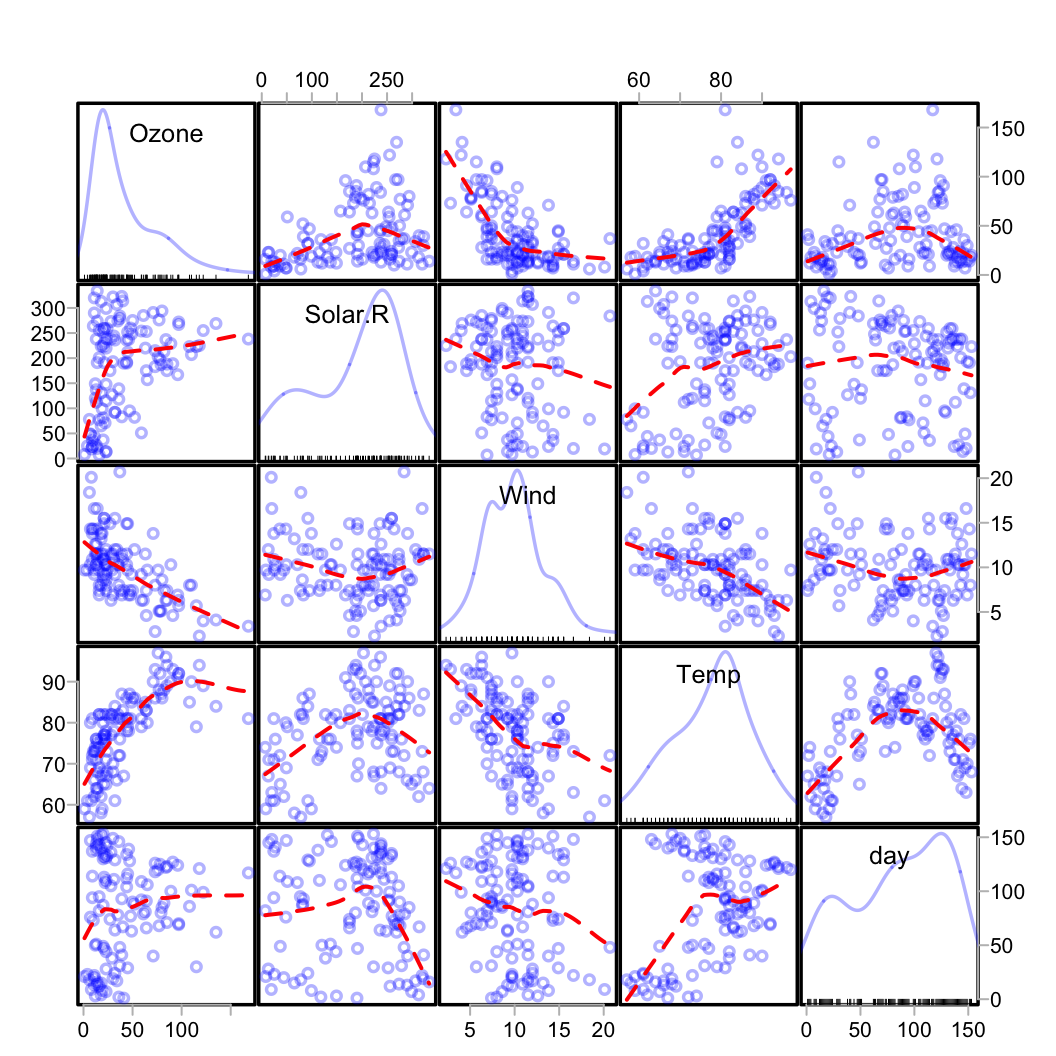
\includegraphics[width=0.8\textwidth,height=\textheight]{figs/g6_11-1.png}
\end{center}

\begin{Shaded}
\begin{Highlighting}[]
\NormalTok{car}\SpecialCharTok{::}\FunctionTok{powerTransform}\NormalTok{(}\FunctionTok{gam}\NormalTok{(Ozone }\SpecialCharTok{\textasciitilde{}} \FunctionTok{s}\NormalTok{(Solar.R)}\SpecialCharTok{+}\FunctionTok{s}\NormalTok{(Wind)}\SpecialCharTok{+}\FunctionTok{s}\NormalTok{(Temp)}\SpecialCharTok{+}\FunctionTok{s}\NormalTok{(day), }\AttributeTok{data=}\NormalTok{airq))}
\end{Highlighting}
\end{Shaded}

\begin{verbatim}
Estimated transformation parameter 
       Y1 
0.2306506 
\end{verbatim}

\begin{Shaded}
\begin{Highlighting}[]
\NormalTok{airq}\SpecialCharTok{$}\NormalTok{rt4Ozone }\OtherTok{\textless{}{-}}\NormalTok{ airq}\SpecialCharTok{$}\NormalTok{Ozone}\SpecialCharTok{\^{}}\FloatTok{0.25}
\end{Highlighting}
\end{Shaded}

\begin{Shaded}
\begin{Highlighting}[]
\NormalTok{Ozone.gam }\OtherTok{\textless{}{-}} \FunctionTok{gam}\NormalTok{(rt4Ozone }\SpecialCharTok{\textasciitilde{}} \FunctionTok{s}\NormalTok{(Solar.R)}\SpecialCharTok{+}\FunctionTok{s}\NormalTok{(Wind)}\SpecialCharTok{+}\FunctionTok{s}\NormalTok{(Temp)}\SpecialCharTok{+}\FunctionTok{s}\NormalTok{(day), }\AttributeTok{data=}\NormalTok{airq)}
\FunctionTok{auto.arima}\NormalTok{(}\FunctionTok{resid}\NormalTok{(Ozone.gam))  }\CommentTok{\# Independent errors model appears OK}
\end{Highlighting}
\end{Shaded}

\begin{verbatim}
Series: resid(Ozone.gam) 
ARIMA(0,0,0) with zero mean 

sigma^2 = 0.05897:  log likelihood = -0.4
AIC=2.79   AICc=2.83   BIC=5.5
\end{verbatim}

\begin{Shaded}
\begin{Highlighting}[]
\DocumentationTok{\#\# Check model terms}
\FunctionTok{anova}\NormalTok{(Ozone.gam)   }\CommentTok{\# For GAM models, this leaves out terms one at a time}
\end{Highlighting}
\end{Shaded}

\begin{verbatim}

Family: gaussian 
Link function: identity 

Formula:
rt4Ozone ~ s(Solar.R) + s(Wind) + s(Temp) + s(day)

Approximate significance of smooth terms:
             edf Ref.df      F  p-value
s(Solar.R) 2.284  2.871  7.701 0.000159
s(Wind)    2.448  3.104  9.497 1.29e-05
s(Temp)    4.275  5.287 13.305  < 2e-16
s(day)     1.000  1.000  0.495 0.483507
\end{verbatim}

\begin{Shaded}
\begin{Highlighting}[]
\DocumentationTok{\#\# The term in \textasciigrave{}day\textasciigrave{} has no explanatory, and will be removed}
\NormalTok{Ozone1.gam }\OtherTok{\textless{}{-}} \FunctionTok{update}\NormalTok{(Ozone.gam, }\AttributeTok{formula=}\NormalTok{rt4Ozone }\SpecialCharTok{\textasciitilde{}} \FunctionTok{s}\NormalTok{(Solar.R)}\SpecialCharTok{+}\FunctionTok{s}\NormalTok{(Wind)}\SpecialCharTok{+}\FunctionTok{s}\NormalTok{(Temp))}
\end{Highlighting}
\end{Shaded}

\subsubsection{Subsection 6.1.9: A calibration problem with time series
errors}\label{subsection-6.1.9-a-calibration-problem-with-time-series-errors}

\begin{Shaded}
\begin{Highlighting}[]
\NormalTok{flakes }\OtherTok{\textless{}{-}}\NormalTok{ DAAG}\SpecialCharTok{::}\NormalTok{frostedflakes}
\NormalTok{calib.arima }\OtherTok{\textless{}{-}} \FunctionTok{with}\NormalTok{(flakes, }\FunctionTok{auto.arima}\NormalTok{(IA400, }\AttributeTok{xreg=}\NormalTok{Lab))}
\NormalTok{calib.arima}
\end{Highlighting}
\end{Shaded}

\begin{verbatim}
Series: IA400 
Regression with ARIMA(0,0,1) errors 

Coefficients:
         ma1  intercept    xreg
      0.3876     6.9235  0.8323
s.e.  0.0859     2.5634  0.0679

sigma^2 = 3.278:  log likelihood = -199.81
AIC=407.62   AICc=408.04   BIC=418.04
\end{verbatim}

\begin{Shaded}
\begin{Highlighting}[]
\FunctionTok{with}\NormalTok{(flakes, }\FunctionTok{coef}\NormalTok{(}\FunctionTok{auto.arima}\NormalTok{(IA400}\SpecialCharTok{/}\NormalTok{Lab, }\AttributeTok{approximation=}\NormalTok{F, }\AttributeTok{stepwise=}\NormalTok{F)))}
\end{Highlighting}
\end{Shaded}

\begin{verbatim}
      ma1 intercept 
0.3718151 1.0173303 
\end{verbatim}

\begin{Shaded}
\begin{Highlighting}[]
\FunctionTok{with}\NormalTok{(flakes, }\FunctionTok{coef}\NormalTok{(}\FunctionTok{auto.arima}\NormalTok{(IA400}\SpecialCharTok{{-}}\NormalTok{Lab, }\AttributeTok{approximation=}\NormalTok{F, }\AttributeTok{stepwise=}\NormalTok{F)))}
\end{Highlighting}
\end{Shaded}

\begin{verbatim}
      ma1 intercept 
0.3838733 0.6201945 
\end{verbatim}

\begin{center}
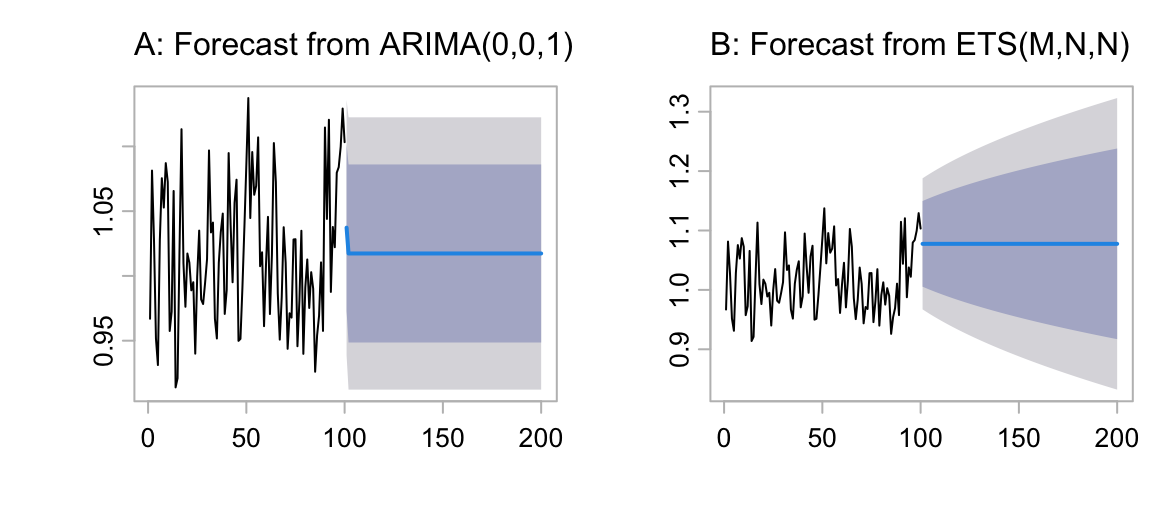
\includegraphics[width=1\textwidth,height=\textheight]{figs/g6_12-1.png}
\end{center}

\subsection{Section 6.2: Nonlinear time
series}\label{section-6.2-nonlinear-time-series}

\begin{Shaded}
\begin{Highlighting}[]
\NormalTok{x }\OtherTok{\textless{}{-}} \FunctionTok{numeric}\NormalTok{(}\DecValTok{999}\NormalTok{)  }\CommentTok{\# x will contain the ARCH(1) errors}
\NormalTok{x0 }\OtherTok{\textless{}{-}} \FunctionTok{rnorm}\NormalTok{(}\DecValTok{1}\NormalTok{)}
\ControlFlowTok{for}\NormalTok{ (i }\ControlFlowTok{in} \DecValTok{1}\SpecialCharTok{:}\DecValTok{999}\NormalTok{)\{}
\NormalTok{x0 }\OtherTok{\textless{}{-}} \FunctionTok{rnorm}\NormalTok{(}\DecValTok{1}\NormalTok{, }\AttributeTok{sd=}\FunctionTok{sqrt}\NormalTok{(.}\DecValTok{25} \SpecialCharTok{+}\NormalTok{ .}\DecValTok{95}\SpecialCharTok{*}\NormalTok{x0}\SpecialCharTok{\^{}}\DecValTok{2}\NormalTok{))}
\NormalTok{x[i] }\OtherTok{\textless{}{-}}\NormalTok{ x0}
\NormalTok{\}}
\end{Highlighting}
\end{Shaded}

\begin{Shaded}
\begin{Highlighting}[]
\FunctionTok{suppressPackageStartupMessages}\NormalTok{(}\FunctionTok{library}\NormalTok{(tseries))}
\FunctionTok{garch}\NormalTok{(x, }\AttributeTok{order =} \FunctionTok{c}\NormalTok{(}\DecValTok{0}\NormalTok{, }\DecValTok{1}\NormalTok{), }\AttributeTok{trace=}\ConstantTok{FALSE}\NormalTok{)}
\end{Highlighting}
\end{Shaded}

\begin{verbatim}

Call:
garch(x = x, order = c(0, 1), trace = FALSE)

Coefficient(s):
    a0      a1  
0.2804  0.9633  
\end{verbatim}

\subsection{Section 6.3: Further
reading}\label{section-6.3-further-reading}

\paragraph{Spatial statistics}\label{spatial-statistics}

\paragraph{Other time series models and
packages}\label{other-time-series-models-and-packages}

\subsection{Section 6.4: Exercises}\label{section-6.4-exercises}

6.4

\begin{Shaded}
\begin{Highlighting}[]
\NormalTok{xx }\OtherTok{\textless{}{-}} \FunctionTok{matrix}\NormalTok{(x, }\AttributeTok{ncol=}\DecValTok{1000}\NormalTok{)}
\end{Highlighting}
\end{Shaded}

6.7

\begin{Shaded}
\begin{Highlighting}[]
\FunctionTok{library}\NormalTok{(tseries)}
\FunctionTok{data}\NormalTok{(ice.river)}
\NormalTok{river1 }\OtherTok{\textless{}{-}} \FunctionTok{diff}\NormalTok{(}\FunctionTok{log}\NormalTok{(ice.river[, }\DecValTok{1}\NormalTok{]))}
\end{Highlighting}
\end{Shaded}

6.9

\begin{Shaded}
\begin{Highlighting}[]
\FunctionTok{library}\NormalTok{(forecast)}
\NormalTok{Eu1 }\OtherTok{\textless{}{-}} \FunctionTok{window}\NormalTok{(EuStockMarkets[,}\DecValTok{1}\NormalTok{], }\AttributeTok{end =} \FunctionTok{c}\NormalTok{(}\DecValTok{1996}\NormalTok{, }\DecValTok{260}\NormalTok{))}
\NormalTok{Eu1nn }\OtherTok{\textless{}{-}} \FunctionTok{nnetar}\NormalTok{(Eu1)}
\NormalTok{Eu1f }\OtherTok{\textless{}{-}} \FunctionTok{forecast}\NormalTok{(Eu1nn, }\AttributeTok{end=}\FunctionTok{end}\NormalTok{(EuStockMarkets[,}\DecValTok{1}\NormalTok{]))}
\FunctionTok{plot}\NormalTok{(Eu1f, }\AttributeTok{ylim=}\FunctionTok{c}\NormalTok{(}\DecValTok{1400}\NormalTok{, }\DecValTok{7000}\NormalTok{))}
\FunctionTok{lines}\NormalTok{(EuStockMarkets[,}\DecValTok{1}\NormalTok{])}
\end{Highlighting}
\end{Shaded}

\begin{center}
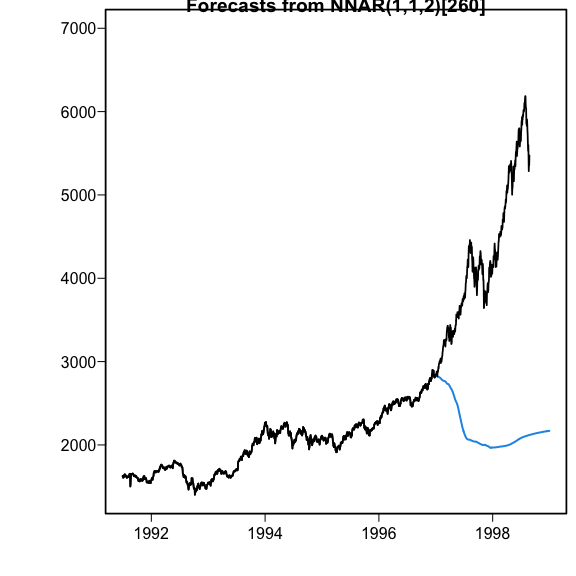
\includegraphics[width=0.8\textwidth,height=\textheight]{figs/gF7d-1.png}
\end{center}

6.10a

\begin{Shaded}
\begin{Highlighting}[]
\NormalTok{airq }\OtherTok{\textless{}{-}} \FunctionTok{cbind}\NormalTok{(airquality[, }\DecValTok{1}\SpecialCharTok{:}\DecValTok{4}\NormalTok{], }\AttributeTok{day=}\DecValTok{1}\SpecialCharTok{:}\FunctionTok{nrow}\NormalTok{(airquality))}
  \CommentTok{\# Column 5 (\textquotesingle{}day\textquotesingle{} starting May 1) replaces columns \textquotesingle{}Month\textquotesingle{} \& \textquotesingle{}Day\textquotesingle{})}
\FunctionTok{library}\NormalTok{(mgcv)}
\NormalTok{temp.gam }\OtherTok{\textless{}{-}} \FunctionTok{gam}\NormalTok{(Temp}\SpecialCharTok{\textasciitilde{}}\FunctionTok{s}\NormalTok{(day), }\AttributeTok{data=}\NormalTok{airq)}
\NormalTok{tempAR1.gamm }\OtherTok{\textless{}{-}} \FunctionTok{gamm}\NormalTok{(Temp}\SpecialCharTok{\textasciitilde{}}\FunctionTok{s}\NormalTok{(day), }\AttributeTok{data=}\NormalTok{airq, }\AttributeTok{correlation=}\FunctionTok{corAR1}\NormalTok{())}
\FunctionTok{plot}\NormalTok{(temp.gam, }\AttributeTok{res=}\NormalTok{T, }\AttributeTok{cex=}\DecValTok{2}\NormalTok{)}
\FunctionTok{plot}\NormalTok{(tempAR1.gamm}\SpecialCharTok{$}\NormalTok{gam, }\AttributeTok{res=}\NormalTok{T, }\AttributeTok{cex=}\DecValTok{2}\NormalTok{)}
\end{Highlighting}
\end{Shaded}

\begin{center}
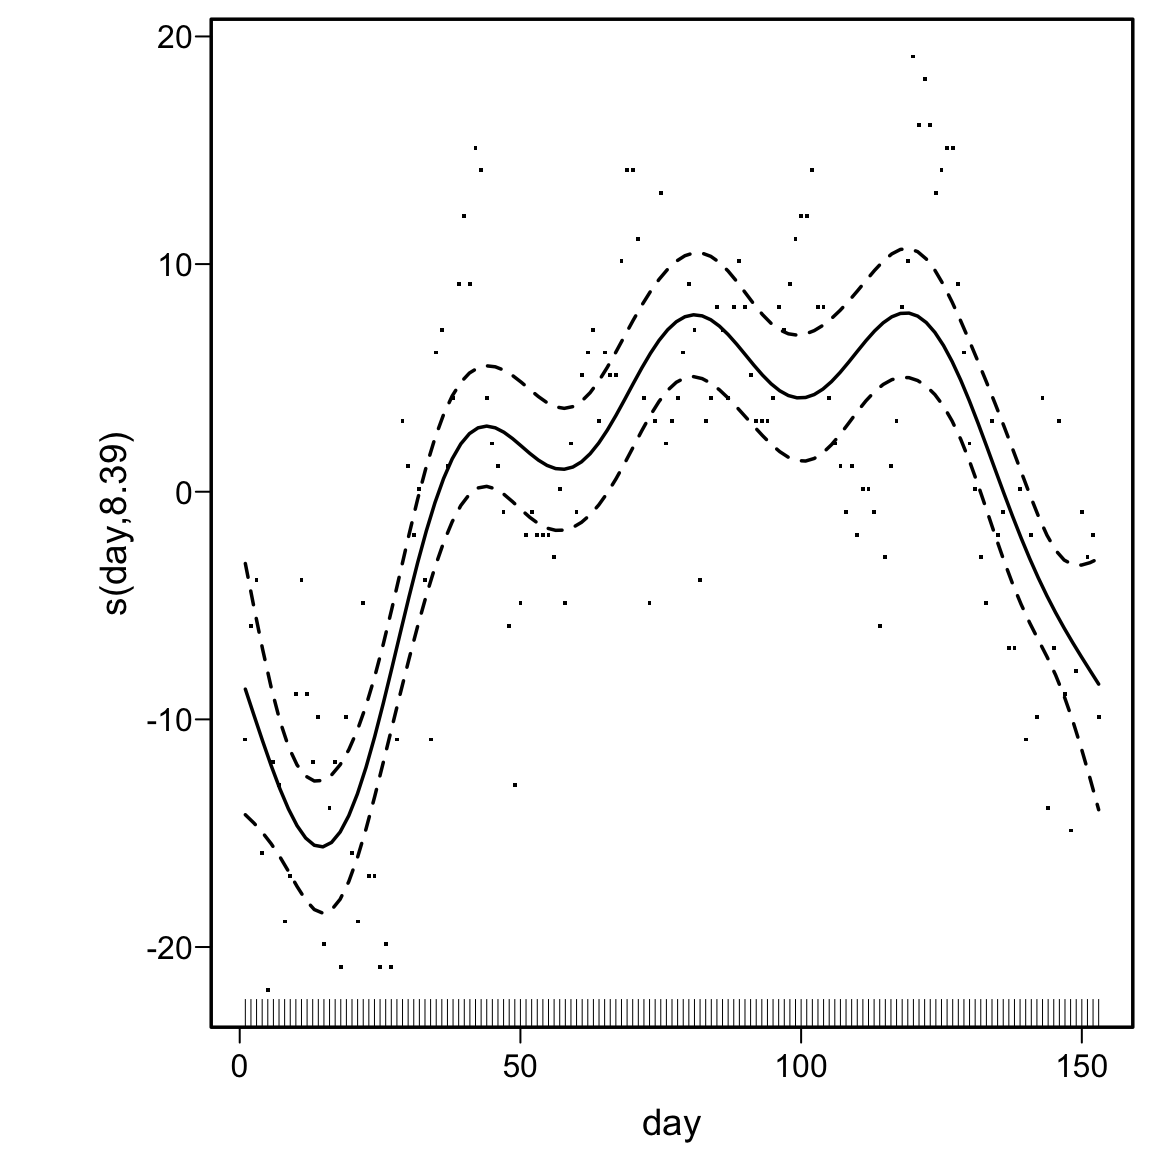
\includegraphics[width=0.8\textwidth,height=\textheight]{figs/gF7e-1.png}
\end{center}

\begin{center}
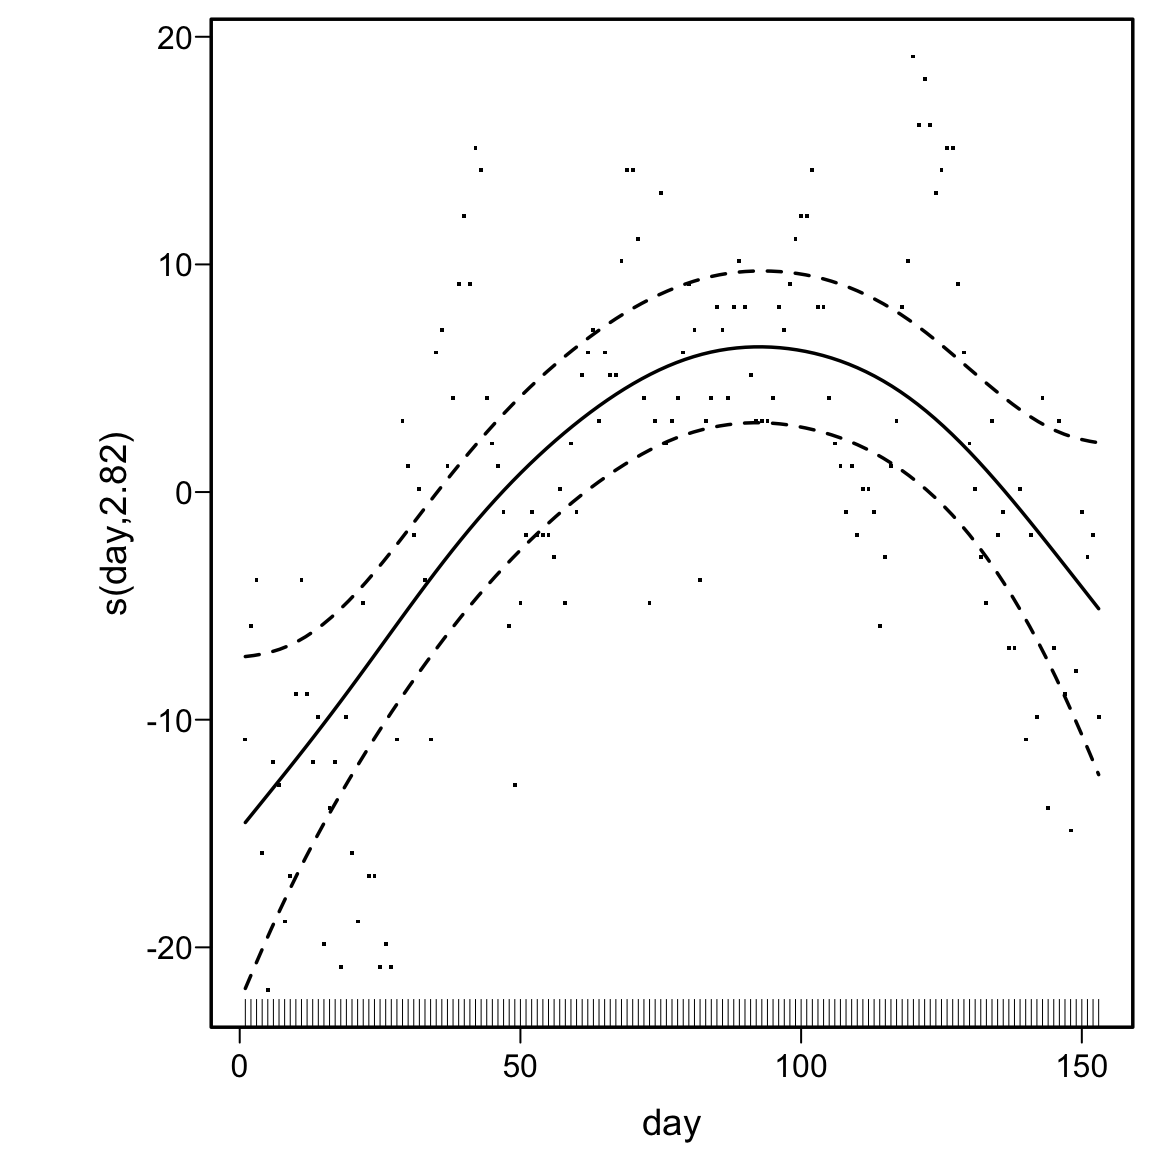
\includegraphics[width=0.8\textwidth,height=\textheight]{figs/gF7e-2.png}
\end{center}

6.10b

\begin{Shaded}
\begin{Highlighting}[]
\NormalTok{(Phi }\OtherTok{\textless{}{-}} \FunctionTok{coef}\NormalTok{(tempAR1.gamm}\SpecialCharTok{$}\NormalTok{lme}\SpecialCharTok{$}\NormalTok{modelStruct}\SpecialCharTok{$}\NormalTok{corStruct, }\AttributeTok{unconstrained =} \ConstantTok{FALSE}\NormalTok{) )}
\NormalTok{Sigma }\OtherTok{\textless{}{-}} \FunctionTok{sqrt}\NormalTok{(tempAR1.gamm}\SpecialCharTok{$}\NormalTok{gam}\SpecialCharTok{$}\NormalTok{sig2)}
\DocumentationTok{\#\# Simulate an AR1 process with this parameter}
\NormalTok{AR1.sim }\OtherTok{\textless{}{-}} \FunctionTok{arima.sim}\NormalTok{(}\AttributeTok{model=}\FunctionTok{list}\NormalTok{(}\AttributeTok{ar=}\NormalTok{Phi), }\AttributeTok{n=}\FunctionTok{nrow}\NormalTok{(airq), }\AttributeTok{sd=}\NormalTok{Sigma)}
\NormalTok{simSeries }\OtherTok{\textless{}{-}}\NormalTok{ AR1.sim}\SpecialCharTok{+}\FunctionTok{fitted}\NormalTok{(tempAR1.gamm}\SpecialCharTok{$}\NormalTok{gam)}
\FunctionTok{plot}\NormalTok{(}\FunctionTok{I}\NormalTok{(}\DecValTok{1}\SpecialCharTok{:}\FunctionTok{nrow}\NormalTok{(airq)), simSeries)}
\DocumentationTok{\#\# Compare with initial series}
\FunctionTok{plot}\NormalTok{(}\FunctionTok{I}\NormalTok{(}\DecValTok{1}\SpecialCharTok{:}\FunctionTok{nrow}\NormalTok{(airq)), airq}\SpecialCharTok{$}\NormalTok{Temp)}
\end{Highlighting}
\end{Shaded}

\begin{Shaded}
\begin{Highlighting}[]
\ControlFlowTok{if}\NormalTok{(}\FunctionTok{file.exists}\NormalTok{(}\StringTok{"/Users/johnm1/pkgs/PGRcode/inst/doc/"}\NormalTok{))\{}
\NormalTok{code }\OtherTok{\textless{}{-}}\NormalTok{ knitr}\SpecialCharTok{::}\NormalTok{knit\_code}\SpecialCharTok{$}\FunctionTok{get}\NormalTok{()}
\NormalTok{txt }\OtherTok{\textless{}{-}} \FunctionTok{paste0}\NormalTok{(}\StringTok{"}\SpecialCharTok{\textbackslash{}n}\StringTok{\#\# "}\NormalTok{, }\FunctionTok{names}\NormalTok{(code),}\StringTok{"}\SpecialCharTok{\textbackslash{}n}\StringTok{"}\NormalTok{, }\FunctionTok{sapply}\NormalTok{(code, paste, }\AttributeTok{collapse=}\StringTok{\textquotesingle{}}\SpecialCharTok{\textbackslash{}n}\StringTok{\textquotesingle{}}\NormalTok{))}
\FunctionTok{writeLines}\NormalTok{(txt, }\AttributeTok{con=}\StringTok{"/Users/johnm1/pkgs/PGRcode/inst/doc/ch6.R"}\NormalTok{)}
\NormalTok{\}}
\end{Highlighting}
\end{Shaded}

\bookmarksetup{startatroot}

\chapter{Chapter 7: Multilevel models, and repeated
measures}\label{chapter-7-multilevel-models-and-repeated-measures}

\paragraph{Packages required (plus any
dependencies)}\label{packages-required-plus-any-dependencies-4}

DAAG lme4 afex MASS utils devtools qra glmmTMB DHARMa MEMSS forecast
splines gamlss plotrix nlme

Additionally, knitr and Hmisc are required in order to process the Rmd
source file.

\begin{Shaded}
\begin{Highlighting}[]
\NormalTok{Hmisc}\SpecialCharTok{::}\FunctionTok{knitrSet}\NormalTok{(}\AttributeTok{basename=}\StringTok{"mva"}\NormalTok{, }\AttributeTok{lang=}\StringTok{\textquotesingle{}markdown\textquotesingle{}}\NormalTok{, }\AttributeTok{fig.path=}\StringTok{"figs/g"}\NormalTok{, }\AttributeTok{w=}\DecValTok{7}\NormalTok{, }\AttributeTok{h=}\DecValTok{7}\NormalTok{)}
\NormalTok{oldopt }\OtherTok{\textless{}{-}} \FunctionTok{options}\NormalTok{(}\AttributeTok{digits=}\DecValTok{4}\NormalTok{, }\AttributeTok{formatR.arrow=}\ConstantTok{FALSE}\NormalTok{, }\AttributeTok{width=}\DecValTok{70}\NormalTok{, }\AttributeTok{scipen=}\DecValTok{999}\NormalTok{)}
\FunctionTok{library}\NormalTok{(knitr)}
\DocumentationTok{\#\# knitr::render\_listings()}
\NormalTok{opts\_chunk[[}\StringTok{\textquotesingle{}set\textquotesingle{}}\NormalTok{]](}\AttributeTok{cache.path=}\StringTok{\textquotesingle{}cache{-}\textquotesingle{}}\NormalTok{, }\AttributeTok{out.width=}\StringTok{"80\%"}\NormalTok{, }\AttributeTok{fig.align=}\StringTok{"center"}\NormalTok{, }
                    \AttributeTok{fig.show=}\StringTok{\textquotesingle{}hold\textquotesingle{}}\NormalTok{, }\AttributeTok{size=}\StringTok{"small"}\NormalTok{, }\AttributeTok{ps=}\DecValTok{10}\NormalTok{, }\AttributeTok{strip.white =} \ConstantTok{TRUE}\NormalTok{,}
                    \AttributeTok{comment=}\ConstantTok{NA}\NormalTok{, }\AttributeTok{width=}\DecValTok{70}\NormalTok{, }\AttributeTok{tidy.opts =} \FunctionTok{list}\NormalTok{(}\AttributeTok{replace.assign=}\ConstantTok{FALSE}\NormalTok{))}
\end{Highlighting}
\end{Shaded}

\subsection{\texorpdfstring{Section 7.1 Corn yield data --- analysis
using
\texttt{aov()}}{Section 7.1 Corn yield data --- analysis using aov()}}\label{section-7.1-corn-yield-data-analysis-using-aov}

\paragraph{Corn yield measurements
example}\label{corn-yield-measurements-example}

\begin{center}
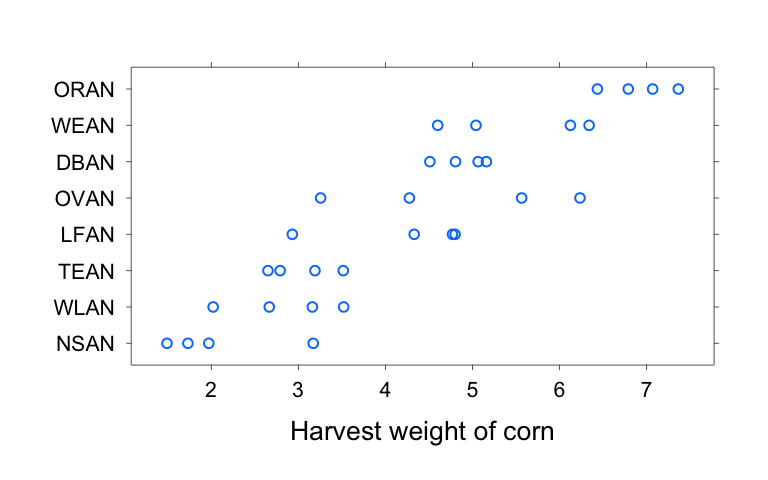
\includegraphics[width=0.65\textwidth,height=\textheight]{figs/g7_1-1.png}
\end{center}

\begin{Shaded}
\begin{Highlighting}[]
\NormalTok{ant111b }\OtherTok{\textless{}{-}} \FunctionTok{within}\NormalTok{(DAAG}\SpecialCharTok{::}\NormalTok{ant111b, Site }\OtherTok{\textless{}{-}} \FunctionTok{reorder}\NormalTok{(site, harvwt, }\AttributeTok{FUN=}\NormalTok{mean))}
\NormalTok{gph }\OtherTok{\textless{}{-}}\NormalTok{ lattice}\SpecialCharTok{::}\FunctionTok{stripplot}\NormalTok{(Site }\SpecialCharTok{\textasciitilde{}}\NormalTok{ harvwt, }\AttributeTok{data=}\NormalTok{ant111b,}
                          \AttributeTok{xlab=}\StringTok{"Harvest weight of corn"}\NormalTok{)}
\FunctionTok{update}\NormalTok{(gph, }\AttributeTok{par.settings=}\NormalTok{DAAG}\SpecialCharTok{::}\FunctionTok{DAAGtheme}\NormalTok{(}\AttributeTok{color=}\ConstantTok{FALSE}\NormalTok{), }\AttributeTok{scales=}\FunctionTok{list}\NormalTok{(}\AttributeTok{tck=}\FloatTok{0.5}\NormalTok{))}
\end{Highlighting}
\end{Shaded}

\begin{Shaded}
\begin{Highlighting}[]
\NormalTok{ant111b }\OtherTok{\textless{}{-}}\NormalTok{ DAAG}\SpecialCharTok{::}\NormalTok{ant111b}
\NormalTok{ant111b.aov }\OtherTok{\textless{}{-}} \FunctionTok{aov}\NormalTok{(harvwt }\SpecialCharTok{\textasciitilde{}} \DecValTok{1} \SpecialCharTok{+} \FunctionTok{Error}\NormalTok{(site), }\AttributeTok{data=}\NormalTok{ant111b)}
\end{Highlighting}
\end{Shaded}

\begin{Shaded}
\begin{Highlighting}[]
\FunctionTok{summary}\NormalTok{(ant111b.aov)}
\end{Highlighting}
\end{Shaded}

\begin{verbatim}

Error: site
          Df Sum Sq Mean Sq F value Pr(>F)
Residuals  7   70.3    10.1               

Error: Within
          Df Sum Sq Mean Sq F value Pr(>F)
Residuals 24   13.9   0.578               
\end{verbatim}

\paragraph{Interpreting the mean
squares}\label{interpreting-the-mean-squares}

\paragraph{Details of the
calculations}\label{details-of-the-calculations}

\paragraph{Practical use of the analysis of variance
results}\label{practical-use-of-the-analysis-of-variance-results}

\paragraph{Random effects vs.~fixed
effects}\label{random-effects-vs.-fixed-effects}

\paragraph{Nested factors -- a variety of
applications}\label{nested-factors-a-variety-of-applications}

\subsubsection{Subsection 7.1.1: A More Formal
Approach}\label{subsection-7.1.1-a-more-formal-approach}

\paragraph{Relations between variance components and mean
squares}\label{relations-between-variance-components-and-mean-squares}

\paragraph{Interpretation of variance
components}\label{interpretation-of-variance-components}

\paragraph{Intra-class correlation}\label{intra-class-correlation}

\subsection{\texorpdfstring{Section 7.2 Analysis using
\texttt{lme4::lmer()}}{Section 7.2 Analysis using lme4::lmer()}}\label{section-7.2-analysis-using-lme4lmer}

\begin{Shaded}
\begin{Highlighting}[]
\FunctionTok{library}\NormalTok{(lme4)}
\NormalTok{ant111b.lmer }\OtherTok{\textless{}{-}} \FunctionTok{lmer}\NormalTok{(harvwt }\SpecialCharTok{\textasciitilde{}} \DecValTok{1} \SpecialCharTok{+}\NormalTok{ (}\DecValTok{1} \SpecialCharTok{|}\NormalTok{ site), }\AttributeTok{data=}\NormalTok{ant111b)}
\end{Highlighting}
\end{Shaded}

\begin{Shaded}
\begin{Highlighting}[]
\DocumentationTok{\#\# Note that there is no degrees of freedom information.}
\FunctionTok{print}\NormalTok{(ant111b.lmer, }\AttributeTok{ranef.comp=}\StringTok{"Variance"}\NormalTok{)}
\end{Highlighting}
\end{Shaded}

\begin{verbatim}
Linear mixed model fit by REML ['lmerMod']
Formula: harvwt ~ 1 + (1 | site)
   Data: ant111b
REML criterion at convergence: 94.42
Random effects:
 Groups   Name        Variance
 site     (Intercept) 2.368   
 Residual             0.578   
Number of obs: 32, groups:  site, 8
Fixed Effects:
(Intercept)  
       4.29  
\end{verbatim}

\paragraph{The processing of output from
lmer()}\label{the-processing-of-output-from-lmer}

\begin{Shaded}
\begin{Highlighting}[]
\FunctionTok{coef}\NormalTok{(}\FunctionTok{summary}\NormalTok{(ant111b.lmer))}
\end{Highlighting}
\end{Shaded}

\begin{verbatim}
            Estimate Std. Error t value
(Intercept)    4.292     0.5604   7.659
\end{verbatim}

\paragraph{Fitted values and residuals in
lmer()}\label{fitted-values-and-residuals-in-lmer}

\begin{Shaded}
\begin{Highlighting}[]
\NormalTok{s2W }\OtherTok{\textless{}{-}} \FloatTok{0.578}\NormalTok{; s2L }\OtherTok{\textless{}{-}} \FloatTok{2.37}\NormalTok{; n }\OtherTok{\textless{}{-}} \DecValTok{4}
\NormalTok{sitemeans }\OtherTok{\textless{}{-}} \FunctionTok{with}\NormalTok{(ant111b, }\FunctionTok{sapply}\NormalTok{(}\FunctionTok{split}\NormalTok{(harvwt, site), mean))}
\NormalTok{grandmean }\OtherTok{\textless{}{-}} \FunctionTok{mean}\NormalTok{(sitemeans)}
\NormalTok{shrinkage }\OtherTok{\textless{}{-}}\NormalTok{ (n}\SpecialCharTok{*}\NormalTok{s2L)}\SpecialCharTok{/}\NormalTok{(n}\SpecialCharTok{*}\NormalTok{s2L}\SpecialCharTok{+}\NormalTok{s2W)}
\DocumentationTok{\#\# Check  that fitted values equal BLUPs, and compare with site means}
\NormalTok{BLUP }\OtherTok{\textless{}{-}}\NormalTok{ grandmean }\SpecialCharTok{+}\NormalTok{ shrinkage}\SpecialCharTok{*}\NormalTok{(sitemeans }\SpecialCharTok{{-}}\NormalTok{ grandmean)}
\NormalTok{BLUP }\OtherTok{\textless{}{-}} \FunctionTok{fitted}\NormalTok{(ant111b.lmer)[}\FunctionTok{match}\NormalTok{(}\FunctionTok{names}\NormalTok{(sitemeans), ant111b}\SpecialCharTok{$}\NormalTok{site)]}
\NormalTok{BLUP }\OtherTok{\textless{}{-}}\NormalTok{ grandmean }\SpecialCharTok{+} \FunctionTok{ranef}\NormalTok{(ant111b.lmer)}\SpecialCharTok{$}\NormalTok{site[[}\DecValTok{1}\NormalTok{]]}
\end{Highlighting}
\end{Shaded}

\begin{Shaded}
\begin{Highlighting}[]
\FunctionTok{rbind}\NormalTok{(}\AttributeTok{BLUP=}\NormalTok{BLUP, }\AttributeTok{sitemeans=}\NormalTok{sitemeans)}
\end{Highlighting}
\end{Shaded}

\begin{verbatim}
           DBAN  LFAN  NSAN  ORAN  OVAN  TEAN  WEAN  WLAN
BLUP      4.851 4.212 2.217 6.764 4.801 3.108 5.455 2.925
sitemeans 4.885 4.207 2.090 6.915 4.833 3.036 5.526 2.841
\end{verbatim}

\paragraph{*Uncertainty in the parameter estimates --- profile
likelihood and
alternatives}\label{uncertainty-in-the-parameter-estimates-profile-likelihood-and-alternatives}

\begin{Shaded}
\begin{Highlighting}[]
\NormalTok{prof.lmer }\OtherTok{\textless{}{-}} \FunctionTok{profile}\NormalTok{(ant111b.lmer)}
\NormalTok{CI95 }\OtherTok{\textless{}{-}} \FunctionTok{confint}\NormalTok{(prof.lmer, }\AttributeTok{level=}\FloatTok{0.95}\NormalTok{)}
\FunctionTok{rbind}\NormalTok{(}\StringTok{"sigmaL\^{}2"}\OtherTok{=}\NormalTok{CI95[}\DecValTok{1}\NormalTok{,]}\SpecialCharTok{\^{}}\DecValTok{2}\NormalTok{, }\StringTok{"sigma\^{}2"}\OtherTok{=}\NormalTok{CI95[}\DecValTok{2}\NormalTok{,]}\SpecialCharTok{\^{}}\DecValTok{2}\NormalTok{)}
\end{Highlighting}
\end{Shaded}

\begin{verbatim}
          2.5 % 97.5 %
sigmaL^2 0.7965  6.936
sigma^2  0.3444  1.079
\end{verbatim}

\begin{Shaded}
\begin{Highlighting}[]
\NormalTok{CI95[}\DecValTok{3}\NormalTok{,]}
\end{Highlighting}
\end{Shaded}

\begin{verbatim}
 2.5 % 97.5 % 
 3.128  5.456 
\end{verbatim}

\begin{center}
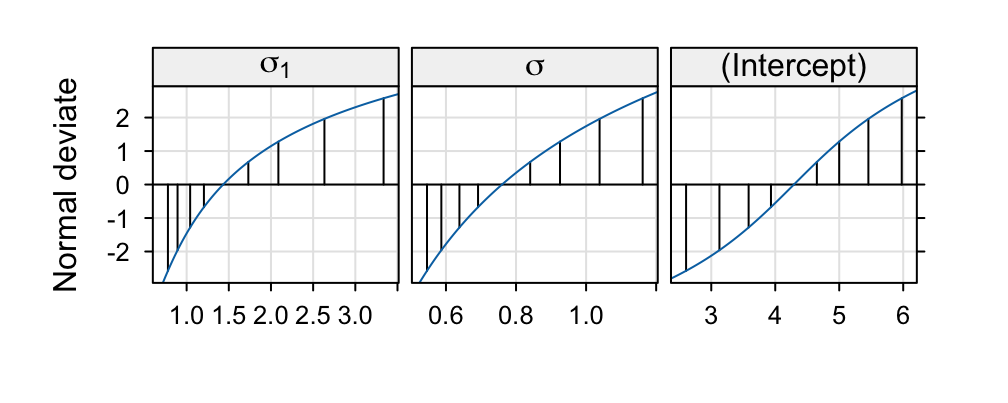
\includegraphics[width=0.85\textwidth,height=\textheight]{figs/g7_2-1.png}
\end{center}

\begin{Shaded}
\begin{Highlighting}[]
\FunctionTok{library}\NormalTok{(lattice)}
\NormalTok{gph }\OtherTok{\textless{}{-}} \FunctionTok{xyplot}\NormalTok{(prof.lmer, }\AttributeTok{conf=}\FunctionTok{c}\NormalTok{(}\DecValTok{50}\NormalTok{, }\DecValTok{80}\NormalTok{, }\DecValTok{95}\NormalTok{, }\DecValTok{99}\NormalTok{)}\SpecialCharTok{/}\DecValTok{100}\NormalTok{,}
              \AttributeTok{aspect=}\FloatTok{0.8}\NormalTok{, }\AttributeTok{between=}\FunctionTok{list}\NormalTok{(}\AttributeTok{x=}\FloatTok{0.35}\NormalTok{))}
\FunctionTok{update}\NormalTok{(gph, }\AttributeTok{scales=}\FunctionTok{list}\NormalTok{(}\AttributeTok{tck=}\FloatTok{0.5}\NormalTok{), }\AttributeTok{ylab=}\StringTok{"Normal deviate"}\NormalTok{)}
\end{Highlighting}
\end{Shaded}

\paragraph{Modeling more than two levels of random
variation}\label{modeling-more-than-two-levels-of-random-variation}

\subsection{Section 7.3 Survey data, with
clustering}\label{section-7.3-survey-data-with-clustering}

\begin{center}
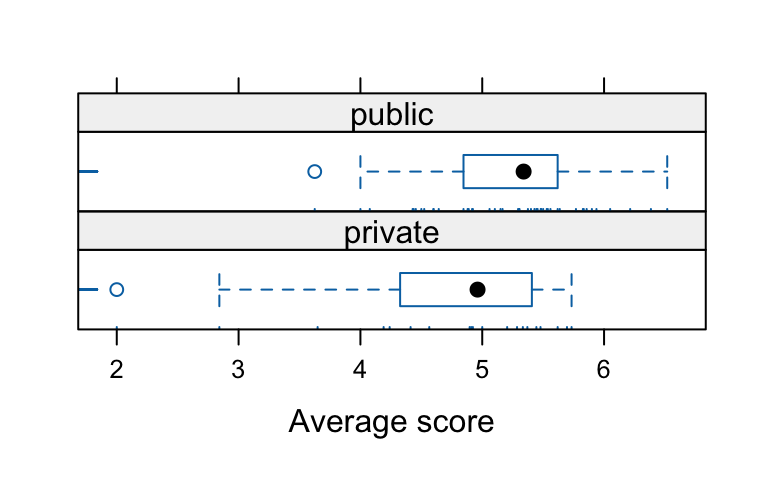
\includegraphics[width=0.65\textwidth,height=\textheight]{figs/g7_3-1.png}
\end{center}

\begin{Shaded}
\begin{Highlighting}[]
\DocumentationTok{\#\# Means of like (data frame science: DAAG), by class}
\NormalTok{science }\OtherTok{\textless{}{-}}\NormalTok{ DAAG}\SpecialCharTok{::}\NormalTok{science}
\NormalTok{classmeans }\OtherTok{\textless{}{-}} \FunctionTok{with}\NormalTok{(science, }\FunctionTok{aggregate}\NormalTok{(like, }\AttributeTok{by=}\FunctionTok{list}\NormalTok{(PrivPub, Class), mean))}
\CommentTok{\# NB: Class identifies classes independently of schools}
\CommentTok{\#     class identifies classes within schools}
\FunctionTok{names}\NormalTok{(classmeans) }\OtherTok{\textless{}{-}} \FunctionTok{c}\NormalTok{(}\StringTok{"PrivPub"}\NormalTok{, }\StringTok{"Class"}\NormalTok{, }\StringTok{"avlike"}\NormalTok{)}
\NormalTok{gph }\OtherTok{\textless{}{-}} \FunctionTok{bwplot}\NormalTok{(}\SpecialCharTok{\textasciitilde{}}\NormalTok{avlike}\SpecialCharTok{|}\NormalTok{PrivPub, }\AttributeTok{layout=}\FunctionTok{c}\NormalTok{(}\DecValTok{1}\NormalTok{,}\DecValTok{2}\NormalTok{), }\AttributeTok{xlab=}\StringTok{"Average score"}\NormalTok{,}
              \AttributeTok{panel=}\ControlFlowTok{function}\NormalTok{(x,y,...)\{}\FunctionTok{panel.bwplot}\NormalTok{(x,y,...)}
              \FunctionTok{panel.rug}\NormalTok{(x,y,...)\}, }\AttributeTok{data=}\NormalTok{classmeans)}
\FunctionTok{update}\NormalTok{(gph, }\AttributeTok{scales=}\FunctionTok{list}\NormalTok{(}\AttributeTok{tcl=}\FloatTok{0.4}\NormalTok{))}
\end{Highlighting}
\end{Shaded}

\subsubsection{Subsection 7.3.1: Alternative
models}\label{subsection-7.3.1-alternative-models}

\begin{Shaded}
\begin{Highlighting}[]
\NormalTok{science }\OtherTok{\textless{}{-}}\NormalTok{ DAAG}\SpecialCharTok{::}\NormalTok{science}
\NormalTok{science.lmer }\OtherTok{\textless{}{-}} \FunctionTok{lmer}\NormalTok{(like }\SpecialCharTok{\textasciitilde{}}\NormalTok{ sex }\SpecialCharTok{+}\NormalTok{ PrivPub }\SpecialCharTok{+}\NormalTok{ (}\DecValTok{1} \SpecialCharTok{|}\NormalTok{ school) }\SpecialCharTok{+}
\NormalTok{                     (}\DecValTok{1} \SpecialCharTok{|}\NormalTok{ school}\SpecialCharTok{:}\NormalTok{class), }\AttributeTok{data =}\NormalTok{ science,}
                     \AttributeTok{na.action=}\NormalTok{na.exclude)}
\end{Highlighting}
\end{Shaded}

\begin{Shaded}
\begin{Highlighting}[]
\FunctionTok{print}\NormalTok{(}\FunctionTok{VarCorr}\NormalTok{(science.lmer), }\AttributeTok{comp=}\StringTok{"Variance"}\NormalTok{, }\AttributeTok{digits=}\DecValTok{2}\NormalTok{)}
\end{Highlighting}
\end{Shaded}

\begin{verbatim}
 Groups       Name        Variance
 school:class (Intercept) 0.32    
 school       (Intercept) 0.00    
 Residual                 3.05    
\end{verbatim}

\begin{Shaded}
\begin{Highlighting}[]
\FunctionTok{print}\NormalTok{(}\FunctionTok{coef}\NormalTok{(}\FunctionTok{summary}\NormalTok{(science.lmer)), }\AttributeTok{digits=}\DecValTok{2}\NormalTok{)}
\end{Highlighting}
\end{Shaded}

\begin{verbatim}
              Estimate Std. Error t value
(Intercept)       4.72      0.162    29.1
sexm              0.18      0.098     1.9
PrivPubpublic     0.41      0.186     2.2
\end{verbatim}

\begin{Shaded}
\begin{Highlighting}[]
\FunctionTok{summary}\NormalTok{(science.lmer)}\SpecialCharTok{$}\NormalTok{ngrps}
\end{Highlighting}
\end{Shaded}

\begin{verbatim}
school:class       school 
          66           41 
\end{verbatim}

\begin{Shaded}
\begin{Highlighting}[]
\NormalTok{science1.lmer }\OtherTok{\textless{}{-}} \FunctionTok{lmer}\NormalTok{(like }\SpecialCharTok{\textasciitilde{}}\NormalTok{ sex }\SpecialCharTok{+}\NormalTok{ PrivPub }\SpecialCharTok{+}\NormalTok{ (}\DecValTok{1} \SpecialCharTok{|}\NormalTok{ school}\SpecialCharTok{:}\NormalTok{class),}
                      \AttributeTok{data =}\NormalTok{ DAAG}\SpecialCharTok{::}\NormalTok{science, }\AttributeTok{na.action=}\NormalTok{na.exclude)}
\end{Highlighting}
\end{Shaded}

\begin{Shaded}
\begin{Highlighting}[]
\FunctionTok{print}\NormalTok{(}\FunctionTok{VarCorr}\NormalTok{(science1.lmer), }\AttributeTok{comp=}\StringTok{"Variance"}\NormalTok{, }\AttributeTok{digits=}\DecValTok{3}\NormalTok{)}
\end{Highlighting}
\end{Shaded}

\begin{verbatim}
 Groups       Name        Variance
 school:class (Intercept) 0.321   
 Residual                 3.052   
\end{verbatim}

\begin{Shaded}
\begin{Highlighting}[]
\FunctionTok{print}\NormalTok{(}\FunctionTok{coef}\NormalTok{(}\FunctionTok{summary}\NormalTok{(science1.lmer)), }\AttributeTok{digits=}\DecValTok{2}\NormalTok{)}
\end{Highlighting}
\end{Shaded}

\begin{verbatim}
              Estimate Std. Error t value
(Intercept)       4.72      0.162    29.1
sexm              0.18      0.098     1.9
PrivPubpublic     0.41      0.186     2.2
\end{verbatim}

\begin{Shaded}
\begin{Highlighting}[]
\NormalTok{opt }\OtherTok{\textless{}{-}} \FunctionTok{options}\NormalTok{(}\AttributeTok{contrasts=}\FunctionTok{c}\NormalTok{(}\StringTok{"contr.sum"}\NormalTok{,}\StringTok{"contr.poly"}\NormalTok{))}
  \CommentTok{\# Change is otherwise made as and if required for individual factors}
  \CommentTok{\# prior to fitting model, and a warning message is generated.}
\NormalTok{afex}\SpecialCharTok{::}\FunctionTok{mixed}\NormalTok{(like }\SpecialCharTok{\textasciitilde{}}\NormalTok{ sex }\SpecialCharTok{+}\NormalTok{ PrivPub }\SpecialCharTok{+}\NormalTok{ (}\DecValTok{1} \SpecialCharTok{|}\NormalTok{ school}\SpecialCharTok{:}\NormalTok{class), }\AttributeTok{method=}\StringTok{"KR"}\NormalTok{, }\AttributeTok{type=}\DecValTok{2}\NormalTok{,}
            \AttributeTok{data =} \FunctionTok{na.omit}\NormalTok{(science),  }\AttributeTok{sig\_symbols=}\FunctionTok{rep}\NormalTok{(}\StringTok{""}\NormalTok{,}\DecValTok{4}\NormalTok{), }\AttributeTok{progress=}\ConstantTok{FALSE}\NormalTok{)}
\end{Highlighting}
\end{Shaded}

\begin{verbatim}
Mixed Model Anova Table (Type 2 tests, KR-method)

Model: like ~ sex + PrivPub + (1 | school:class)
Data: na.omit(science)
   Effect         df    F p.value
1     sex 1, 1379.49 3.44    .064
2 PrivPub   1, 60.44 4.91    .030
\end{verbatim}

\begin{Shaded}
\begin{Highlighting}[]
\FunctionTok{options}\NormalTok{(opt)       }\CommentTok{\# Reset to previous contrasts setting}
\end{Highlighting}
\end{Shaded}

\paragraph{More detailed examination of the
output}\label{more-detailed-examination-of-the-output}

\begin{Shaded}
\begin{Highlighting}[]
\DocumentationTok{\#\# Use profile likelihood}
\NormalTok{pp }\OtherTok{\textless{}{-}} \FunctionTok{profile}\NormalTok{(science1.lmer, }\AttributeTok{which=}\StringTok{"theta\_"}\NormalTok{)}
\CommentTok{\# which="theta\_": all random parameters}
\CommentTok{\# which="beta\_": fixed effect parameters}
\NormalTok{var95 }\OtherTok{\textless{}{-}} \FunctionTok{confint}\NormalTok{(pp, }\AttributeTok{level=}\FloatTok{0.95}\NormalTok{)}\SpecialCharTok{\^{}}\DecValTok{2}
\CommentTok{\# Square to get variances in place of SDs}
\FunctionTok{rownames}\NormalTok{(var95) }\OtherTok{\textless{}{-}} \FunctionTok{c}\NormalTok{(}\StringTok{"sigma\_Class\^{}2"}\NormalTok{, }\StringTok{"sigma\^{}2"}\NormalTok{)}
\FunctionTok{signif}\NormalTok{(var95, }\DecValTok{3}\NormalTok{)}
\end{Highlighting}
\end{Shaded}

\begin{verbatim}
              2.5 % 97.5 %
sigma_Class^2 0.178  0.511
sigma^2       2.830  3.300
\end{verbatim}

\begin{Shaded}
\begin{Highlighting}[]
\DocumentationTok{\#\# Fit model and generate quantities that will be plotted}
\NormalTok{science1.lmer }\OtherTok{\textless{}{-}} \FunctionTok{lmer}\NormalTok{(like }\SpecialCharTok{\textasciitilde{}}\NormalTok{ sex }\SpecialCharTok{+}\NormalTok{ PrivPub }\SpecialCharTok{+}\NormalTok{ (}\DecValTok{1} \SpecialCharTok{|}\NormalTok{ school}\SpecialCharTok{:}\NormalTok{class),}
\AttributeTok{data =}\NormalTok{ science, }\AttributeTok{na.action=}\NormalTok{na.omit)}
\DocumentationTok{\#\# Panel A: random site effects vs number in class}
\NormalTok{ranf }\OtherTok{\textless{}{-}} \FunctionTok{ranef}\NormalTok{(}\AttributeTok{obj =}\NormalTok{ science1.lmer, }\AttributeTok{drop=}\ConstantTok{TRUE}\NormalTok{)[[}\StringTok{"school:class"}\NormalTok{]]}
\NormalTok{flist }\OtherTok{\textless{}{-}}\NormalTok{ science1.lmer}\SpecialCharTok{@}\NormalTok{flist[[}\StringTok{"school:class"}\NormalTok{]]}
\NormalTok{privpub }\OtherTok{\textless{}{-}}\NormalTok{ science[}\FunctionTok{match}\NormalTok{(}\FunctionTok{names}\NormalTok{(ranf), flist), }\StringTok{"PrivPub"}\NormalTok{]}
\NormalTok{num }\OtherTok{\textless{}{-}} \FunctionTok{unclass}\NormalTok{(}\FunctionTok{table}\NormalTok{(flist)); numlabs }\OtherTok{\textless{}{-}} \FunctionTok{pretty}\NormalTok{(num)}
\DocumentationTok{\#\# Panel B: Within class variance estimates vs numbers}
\NormalTok{res }\OtherTok{\textless{}{-}} \FunctionTok{residuals}\NormalTok{(science1.lmer)}
\NormalTok{vars }\OtherTok{\textless{}{-}} \FunctionTok{tapply}\NormalTok{(res, }\AttributeTok{INDEX=}\FunctionTok{list}\NormalTok{(flist), }\AttributeTok{FUN=}\NormalTok{var)}\SpecialCharTok{*}\NormalTok{(num}\DecValTok{{-}1}\NormalTok{)}\SpecialCharTok{/}\NormalTok{(num}\DecValTok{{-}2}\NormalTok{)}
\DocumentationTok{\#\# Panel C: Normal probability of random site effects (\textasciigrave{}ranf\textasciigrave{})}
\DocumentationTok{\#\# Panel D: Normal probability of residuals (\textasciigrave{}res\textasciigrave{})}
\end{Highlighting}
\end{Shaded}

\begin{center}
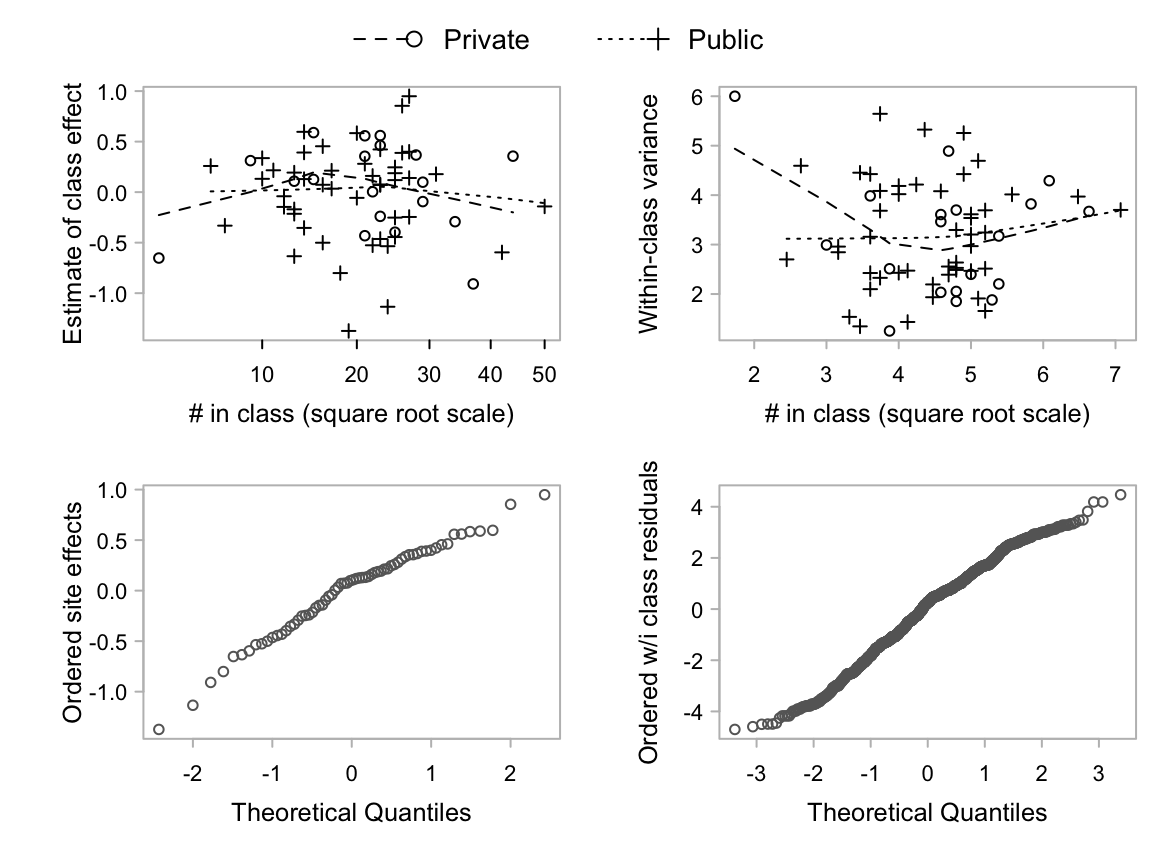
\includegraphics[width=1\textwidth,height=\textheight]{figs/g7_4-1.png}
\end{center}

\begin{Shaded}
\begin{Highlighting}[]
\NormalTok{opar }\OtherTok{\textless{}{-}} \FunctionTok{par}\NormalTok{(}\AttributeTok{oma=}\FunctionTok{c}\NormalTok{(}\DecValTok{0}\NormalTok{,}\DecValTok{0}\NormalTok{,}\FloatTok{1.5}\NormalTok{,}\DecValTok{0}\NormalTok{))}
\DocumentationTok{\#\# Panel A: Plot effect estimates vs number}
\NormalTok{xlab12 }\OtherTok{\textless{}{-}} \StringTok{"\# in class (square root scale)"}
\FunctionTok{plot}\NormalTok{(}\FunctionTok{sqrt}\NormalTok{(num), ranf, }\AttributeTok{xaxt=}\StringTok{"n"}\NormalTok{, }\AttributeTok{pch=}\FunctionTok{c}\NormalTok{(}\DecValTok{1}\NormalTok{,}\DecValTok{3}\NormalTok{)[}\FunctionTok{as.numeric}\NormalTok{(privpub)], }\AttributeTok{cex=}\FloatTok{0.8}\NormalTok{,}
     \AttributeTok{xlab=}\NormalTok{xlab12, }\AttributeTok{ylab=}\StringTok{"Estimate of class effect"}\NormalTok{, }\AttributeTok{fg=}\StringTok{"gray"}\NormalTok{)}
\FunctionTok{lines}\NormalTok{(}\FunctionTok{lowess}\NormalTok{(}\FunctionTok{sqrt}\NormalTok{(num[privpub}\SpecialCharTok{==}\StringTok{"private"}\NormalTok{]),}
\NormalTok{ranf[privpub}\SpecialCharTok{==}\StringTok{"private"}\NormalTok{], }\AttributeTok{f=}\FloatTok{1.1}\NormalTok{), }\AttributeTok{lty=}\DecValTok{2}\NormalTok{)}
\FunctionTok{lines}\NormalTok{(}\FunctionTok{lowess}\NormalTok{(}\FunctionTok{sqrt}\NormalTok{(num[privpub}\SpecialCharTok{==}\StringTok{"public"}\NormalTok{]),}
\NormalTok{ranf[privpub}\SpecialCharTok{==}\StringTok{"public"}\NormalTok{], }\AttributeTok{f=}\FloatTok{1.1}\NormalTok{), }\AttributeTok{lty=}\DecValTok{3}\NormalTok{)}
\FunctionTok{axis}\NormalTok{(}\DecValTok{1}\NormalTok{, }\AttributeTok{at=}\FunctionTok{sqrt}\NormalTok{(numlabs), }\AttributeTok{labels=}\FunctionTok{paste}\NormalTok{(numlabs), }\AttributeTok{lwd=}\DecValTok{0}\NormalTok{, }\AttributeTok{lwd.ticks=}\DecValTok{1}\NormalTok{)}
\DocumentationTok{\#\# Panel B: Within class variance estimates vs numbers}
\FunctionTok{plot}\NormalTok{(}\FunctionTok{sqrt}\NormalTok{(num), vars, }\AttributeTok{pch=}\FunctionTok{c}\NormalTok{(}\DecValTok{1}\NormalTok{,}\DecValTok{3}\NormalTok{)[}\FunctionTok{unclass}\NormalTok{(privpub)], }\AttributeTok{cex=}\FloatTok{0.8}\NormalTok{,}
     \AttributeTok{xlab=}\NormalTok{xlab12, }\AttributeTok{ylab=}\StringTok{"Within{-}class variance"}\NormalTok{, }\AttributeTok{fg=}\StringTok{"gray"}\NormalTok{)}
\FunctionTok{lines}\NormalTok{(}\FunctionTok{lowess}\NormalTok{(}\FunctionTok{sqrt}\NormalTok{(num[privpub}\SpecialCharTok{==}\StringTok{"private"}\NormalTok{]),}
      \FunctionTok{as.vector}\NormalTok{(vars)[privpub}\SpecialCharTok{==}\StringTok{"private"}\NormalTok{], }\AttributeTok{f=}\FloatTok{1.1}\NormalTok{), }\AttributeTok{lty=}\DecValTok{2}\NormalTok{)}
\FunctionTok{lines}\NormalTok{(}\FunctionTok{lowess}\NormalTok{(}\FunctionTok{sqrt}\NormalTok{(num[privpub}\SpecialCharTok{==}\StringTok{"public"}\NormalTok{]),}
\FunctionTok{as.vector}\NormalTok{(vars)[privpub}\SpecialCharTok{==}\StringTok{"public"}\NormalTok{], }\AttributeTok{f=}\FloatTok{1.1}\NormalTok{), }\AttributeTok{lty=}\DecValTok{3}\NormalTok{)}
\DocumentationTok{\#\# Panel C: Normal quantile{-}quantile plot of site effects}
\FunctionTok{qqnorm}\NormalTok{(ranf, }\AttributeTok{ylab=}\StringTok{"Ordered site effects"}\NormalTok{, }\AttributeTok{cex=}\FloatTok{0.8}\NormalTok{, }\AttributeTok{main=}\StringTok{""}\NormalTok{,}
       \AttributeTok{col=}\StringTok{"gray40"}\NormalTok{, }\AttributeTok{fg=}\StringTok{"gray"}\NormalTok{)}
\DocumentationTok{\#\# Panel D: Normal quantile{-}quantile plot of residuals}
\FunctionTok{qqnorm}\NormalTok{(res, }\AttributeTok{ylab=}\StringTok{"Ordered w/i class residuals"}\NormalTok{, }\AttributeTok{cex=}\FloatTok{0.8}\NormalTok{, }\AttributeTok{main=}\StringTok{""}\NormalTok{,}
       \AttributeTok{col=}\StringTok{"gray40"}\NormalTok{, }\AttributeTok{fg=}\StringTok{"gray"}\NormalTok{)}
\FunctionTok{par}\NormalTok{(}\AttributeTok{fig =} \FunctionTok{c}\NormalTok{(}\DecValTok{0}\NormalTok{, }\DecValTok{1}\NormalTok{, }\DecValTok{0}\NormalTok{, }\DecValTok{1}\NormalTok{), }\AttributeTok{oma =} \FunctionTok{c}\NormalTok{(}\DecValTok{0}\NormalTok{, }\DecValTok{0}\NormalTok{, }\DecValTok{0}\NormalTok{, }\DecValTok{0}\NormalTok{), }\AttributeTok{mar =} \FunctionTok{c}\NormalTok{(}\DecValTok{0}\NormalTok{, }\DecValTok{0}\NormalTok{, }\DecValTok{0}\NormalTok{, }\DecValTok{0}\NormalTok{),}
\AttributeTok{new =} \ConstantTok{TRUE}\NormalTok{)}
\FunctionTok{plot}\NormalTok{(}\DecValTok{0}\NormalTok{, }\DecValTok{0}\NormalTok{, }\AttributeTok{type =} \StringTok{"n"}\NormalTok{, }\AttributeTok{bty =} \StringTok{"n"}\NormalTok{, }\AttributeTok{xaxt =} \StringTok{"n"}\NormalTok{, }\AttributeTok{yaxt =} \StringTok{"n"}\NormalTok{)}
\FunctionTok{legend}\NormalTok{(}\AttributeTok{x=}\StringTok{"top"}\NormalTok{, }\AttributeTok{legend=}\FunctionTok{c}\NormalTok{(}\StringTok{"Private     "}\NormalTok{, }\StringTok{"Public"}\NormalTok{), }\AttributeTok{pch=}\FunctionTok{c}\NormalTok{(}\DecValTok{1}\NormalTok{,}\DecValTok{3}\NormalTok{),}
       \AttributeTok{lwd=}\FunctionTok{c}\NormalTok{(}\DecValTok{1}\NormalTok{,}\DecValTok{1}\NormalTok{), }\AttributeTok{lty=}\DecValTok{2}\SpecialCharTok{:}\DecValTok{3}\NormalTok{, }\AttributeTok{cex=}\FloatTok{1.25}\NormalTok{,}
       \AttributeTok{xjust=}\FloatTok{0.5}\NormalTok{, }\AttributeTok{yjust=}\FloatTok{0.8}\NormalTok{, }\AttributeTok{horiz=}\ConstantTok{TRUE}\NormalTok{, }\AttributeTok{merge=}\ConstantTok{FALSE}\NormalTok{, }\AttributeTok{bty=}\StringTok{"n"}\NormalTok{)}
\FunctionTok{par}\NormalTok{(opar)}
\end{Highlighting}
\end{Shaded}

\subsubsection{Subsection 7.3.2: Instructive, though faulty,
analyses}\label{subsection-7.3.2-instructive-though-faulty-analyses}

\paragraph{Ignoring class as the random
effect}\label{ignoring-class-as-the-random-effect}

\begin{Shaded}
\begin{Highlighting}[]
\NormalTok{science2.lmer }\OtherTok{\textless{}{-}} \FunctionTok{lmer}\NormalTok{(like }\SpecialCharTok{\textasciitilde{}}\NormalTok{ sex }\SpecialCharTok{+}\NormalTok{ PrivPub }\SpecialCharTok{+}\NormalTok{ (}\DecValTok{1} \SpecialCharTok{|}\NormalTok{ school),}
\AttributeTok{data =}\NormalTok{ science, }\AttributeTok{na.action=}\NormalTok{na.exclude)}
\FunctionTok{print}\NormalTok{(}\FunctionTok{coef}\NormalTok{(}\FunctionTok{summary}\NormalTok{(science2.lmer)), }\AttributeTok{digits=}\DecValTok{3}\NormalTok{)}
\end{Highlighting}
\end{Shaded}

\begin{verbatim}
              Estimate Std. Error t value
(Intercept)      4.738      0.163   29.00
sexm             0.197      0.101    1.96
PrivPubpublic    0.417      0.185    2.25
\end{verbatim}

\begin{Shaded}
\begin{Highlighting}[]
\DocumentationTok{\#\# NB: Output is misleading}
\FunctionTok{print}\NormalTok{(}\FunctionTok{VarCorr}\NormalTok{(science2.lmer), }\AttributeTok{comp=}\StringTok{"Variance"}\NormalTok{, }\AttributeTok{digits=}\DecValTok{3}\NormalTok{)}
\end{Highlighting}
\end{Shaded}

\begin{verbatim}
 Groups   Name        Variance
 school   (Intercept) 0.166   
 Residual             3.219   
\end{verbatim}

\paragraph{Ignoring the random structure in the
data}\label{ignoring-the-random-structure-in-the-data}

\begin{Shaded}
\begin{Highlighting}[]
\DocumentationTok{\#\# Faulty analysis, using lm}
\NormalTok{science.lm }\OtherTok{\textless{}{-}} \FunctionTok{lm}\NormalTok{(like }\SpecialCharTok{\textasciitilde{}}\NormalTok{ sex }\SpecialCharTok{+}\NormalTok{ PrivPub, }\AttributeTok{data=}\NormalTok{science)}
\FunctionTok{round}\NormalTok{(}\FunctionTok{coef}\NormalTok{(}\FunctionTok{summary}\NormalTok{(science.lm)), }\AttributeTok{digits=}\DecValTok{4}\NormalTok{)}
\end{Highlighting}
\end{Shaded}

\begin{verbatim}
              Estimate Std. Error t value Pr(>|t|)
(Intercept)     4.7402     0.0996  47.616   0.0000
sexm            0.1509     0.0986   1.531   0.1261
PrivPubpublic   0.3951     0.1051   3.759   0.0002
\end{verbatim}

\subsubsection{Subsection 7.3.3: Predictive
accuracy}\label{subsection-7.3.3-predictive-accuracy}

\subsection{Section 7.4 A multilevel experimental
design}\label{section-7.4-a-multilevel-experimental-design}

\begin{center}
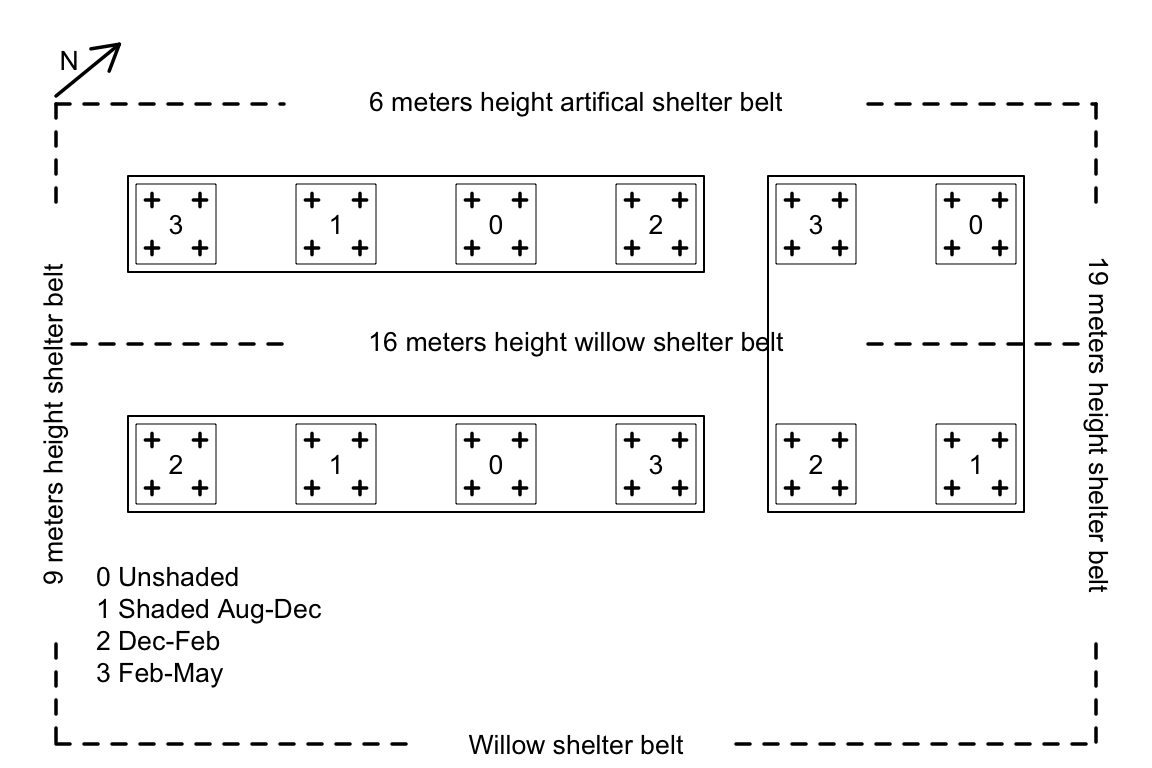
\includegraphics[width=1\textwidth,height=\textheight]{figs/g7_5-1.png}
\end{center}

\begin{Shaded}
\begin{Highlighting}[]
\FunctionTok{par}\NormalTok{(}\AttributeTok{mar=}\FunctionTok{rep}\NormalTok{(}\FloatTok{0.25}\NormalTok{,}\DecValTok{4}\NormalTok{))}
\NormalTok{MASS}\SpecialCharTok{::}\FunctionTok{eqscplot}\NormalTok{(}\FunctionTok{c}\NormalTok{(}\DecValTok{0}\NormalTok{,}\DecValTok{13}\NormalTok{),}\FunctionTok{c}\NormalTok{(}\FloatTok{4.0}\NormalTok{,}\DecValTok{13}\NormalTok{),}\AttributeTok{type=}\StringTok{"n"}\NormalTok{,}\AttributeTok{xlab=}\StringTok{""}\NormalTok{,}\AttributeTok{ylab=}\StringTok{""}\NormalTok{, }\AttributeTok{asp=}\DecValTok{1}\NormalTok{, }\AttributeTok{axes=}\NormalTok{F)}
\NormalTok{eps }\OtherTok{\textless{}{-}} \FloatTok{0.1}
\NormalTok{suby }\OtherTok{\textless{}{-}} \DecValTok{12}
\NormalTok{vines}\OtherTok{\textless{}{-}}\ControlFlowTok{function}\NormalTok{(}\AttributeTok{x=}\DecValTok{1}\NormalTok{,}\AttributeTok{y=}\DecValTok{1}\NormalTok{,}\AttributeTok{subp=}\DecValTok{0}\NormalTok{, }\AttributeTok{suby=}\DecValTok{12}\NormalTok{)\{}
\FunctionTok{lines}\NormalTok{(}\FunctionTok{c}\NormalTok{(y,y,y}\SpecialCharTok{+}\DecValTok{1}\NormalTok{,y}\SpecialCharTok{+}\DecValTok{1}\NormalTok{,y), suby}\SpecialCharTok{{-}}\FunctionTok{c}\NormalTok{(x,x}\SpecialCharTok{+}\DecValTok{1}\NormalTok{,x}\SpecialCharTok{+}\DecValTok{1}\NormalTok{,x,x),}\AttributeTok{lwd=}\FloatTok{0.5}\NormalTok{)}
\FunctionTok{points}\NormalTok{(}\FunctionTok{c}\NormalTok{(y}\FloatTok{+.2}\NormalTok{,y}\FloatTok{+.2}\NormalTok{,y}\FloatTok{+.8}\NormalTok{,y}\FloatTok{+.8}\NormalTok{),suby}\SpecialCharTok{{-}}\FunctionTok{c}\NormalTok{(x}\FloatTok{+.2}\NormalTok{,x}\FloatTok{+.8}\NormalTok{,x}\FloatTok{+.8}\NormalTok{,x}\FloatTok{+.2}\NormalTok{),}\AttributeTok{pch=}\DecValTok{3}\NormalTok{,}\AttributeTok{cex=}\FloatTok{0.65}\NormalTok{)}
\FunctionTok{text}\NormalTok{(y}\FloatTok{+.5}\NormalTok{,suby}\SpecialCharTok{{-}}\NormalTok{(x}\FloatTok{+.5}\NormalTok{),}\FunctionTok{paste}\NormalTok{(subp))}
\NormalTok{\}}
\NormalTok{k}\OtherTok{\textless{}{-}}\DecValTok{0}
\ControlFlowTok{for}\NormalTok{(i }\ControlFlowTok{in} \FunctionTok{c}\NormalTok{(}\DecValTok{1}\NormalTok{,}\DecValTok{3}\NormalTok{,}\DecValTok{5}\NormalTok{,}\DecValTok{7}\NormalTok{))\{k}\OtherTok{\textless{}{-}}\NormalTok{k}\SpecialCharTok{+}\DecValTok{1}\NormalTok{; }\FunctionTok{vines}\NormalTok{(}\DecValTok{1}\NormalTok{,i,}\FunctionTok{c}\NormalTok{(}\DecValTok{3}\NormalTok{,}\DecValTok{1}\NormalTok{,}\DecValTok{0}\NormalTok{,}\DecValTok{2}\NormalTok{)[k])\}}
\NormalTok{k}\OtherTok{\textless{}{-}}\DecValTok{0}
\ControlFlowTok{for}\NormalTok{(i }\ControlFlowTok{in} \FunctionTok{c}\NormalTok{(}\DecValTok{1}\NormalTok{,}\DecValTok{3}\NormalTok{,}\DecValTok{5}\NormalTok{,}\DecValTok{7}\NormalTok{))\{k}\OtherTok{\textless{}{-}}\NormalTok{k}\SpecialCharTok{+}\DecValTok{1}\NormalTok{; }\FunctionTok{vines}\NormalTok{(}\DecValTok{4}\NormalTok{,i,}\FunctionTok{c}\NormalTok{(}\DecValTok{2}\NormalTok{,}\DecValTok{1}\NormalTok{,}\DecValTok{0}\NormalTok{,}\DecValTok{3}\NormalTok{)[k])\}}
\NormalTok{k }\OtherTok{\textless{}{-}} \DecValTok{0}
\ControlFlowTok{for}\NormalTok{(i }\ControlFlowTok{in} \FunctionTok{c}\NormalTok{(}\DecValTok{1}\NormalTok{,}\DecValTok{4}\NormalTok{,}\DecValTok{4}\NormalTok{,}\DecValTok{1}\NormalTok{))\{k}\OtherTok{\textless{}{-}}\NormalTok{k}\SpecialCharTok{+}\DecValTok{1}
\NormalTok{j}\OtherTok{\textless{}{-}}\FunctionTok{c}\NormalTok{(}\DecValTok{9}\NormalTok{,}\DecValTok{9}\NormalTok{,}\DecValTok{11}\NormalTok{,}\DecValTok{11}\NormalTok{)[k]}
\FunctionTok{vines}\NormalTok{(i,j,}\FunctionTok{c}\NormalTok{(}\DecValTok{3}\NormalTok{,}\DecValTok{2}\NormalTok{,}\DecValTok{1}\NormalTok{,}\DecValTok{0}\NormalTok{)[k])}
\NormalTok{\}}
\FunctionTok{lines}\NormalTok{(}\FunctionTok{c}\NormalTok{(}\DecValTok{2}\SpecialCharTok{*}\NormalTok{eps,}\FloatTok{2.85}\NormalTok{,}\ConstantTok{NA}\NormalTok{,}\FloatTok{10.15}\NormalTok{,}\DecValTok{13{-}2}\SpecialCharTok{*}\NormalTok{eps), suby}\SpecialCharTok{{-}}\FunctionTok{c}\NormalTok{(}\DecValTok{3}\NormalTok{,}\DecValTok{3}\NormalTok{,}\ConstantTok{NA}\NormalTok{,}\DecValTok{3}\NormalTok{,}\DecValTok{3}\NormalTok{),}\AttributeTok{lty=}\DecValTok{2}\NormalTok{)}
\FunctionTok{lines}\NormalTok{(}\FunctionTok{c}\NormalTok{(}\DecValTok{0}\NormalTok{,}\FloatTok{2.85}\NormalTok{,}\ConstantTok{NA}\NormalTok{,}\FloatTok{10.15}\NormalTok{,}\DecValTok{13}\NormalTok{),suby}\SpecialCharTok{{-}}\FunctionTok{c}\NormalTok{(}\DecValTok{0}\NormalTok{,}\DecValTok{0}\NormalTok{,}\ConstantTok{NA}\NormalTok{,}\DecValTok{0}\NormalTok{,}\DecValTok{0}\NormalTok{),}\AttributeTok{lty=}\DecValTok{2}\NormalTok{)}
\FunctionTok{lines}\NormalTok{(}\FunctionTok{c}\NormalTok{(}\DecValTok{0}\NormalTok{,}\FloatTok{4.5}\NormalTok{,}\ConstantTok{NA}\NormalTok{,}\FloatTok{8.5}\NormalTok{,}\DecValTok{13}\NormalTok{),suby}\SpecialCharTok{{-}}\FunctionTok{c}\NormalTok{(}\DecValTok{8}\NormalTok{,}\DecValTok{8}\NormalTok{,}\ConstantTok{NA}\NormalTok{,}\DecValTok{8}\NormalTok{,}\DecValTok{8}\NormalTok{),}\AttributeTok{lty=}\DecValTok{2}\NormalTok{)}
\FunctionTok{lines}\NormalTok{(}\FunctionTok{rep}\NormalTok{(}\DecValTok{0}\NormalTok{,}\DecValTok{5}\NormalTok{),suby}\SpecialCharTok{{-}}\FunctionTok{c}\NormalTok{(}\DecValTok{0}\NormalTok{,}\FloatTok{1.25}\NormalTok{,}\ConstantTok{NA}\NormalTok{,}\FloatTok{6.75}\NormalTok{,}\DecValTok{8}\NormalTok{),}\AttributeTok{lty=}\DecValTok{2}\NormalTok{)}
\FunctionTok{lines}\NormalTok{(}\FunctionTok{rep}\NormalTok{(}\DecValTok{13}\NormalTok{,}\DecValTok{5}\NormalTok{),suby}\SpecialCharTok{{-}}\FunctionTok{c}\NormalTok{(}\DecValTok{0}\NormalTok{,}\FloatTok{1.25}\NormalTok{,}\ConstantTok{NA}\NormalTok{,}\FloatTok{6.75}\NormalTok{,}\DecValTok{8}\NormalTok{),}\AttributeTok{lty=}\DecValTok{2}\NormalTok{)}
\FunctionTok{lines}\NormalTok{(}\FunctionTok{c}\NormalTok{(}\DecValTok{9}\NormalTok{,}\DecValTok{9}\NormalTok{,}\DecValTok{12}\NormalTok{,}\DecValTok{12}\NormalTok{,}\DecValTok{9}\NormalTok{)}\SpecialCharTok{+}\FunctionTok{c}\NormalTok{(}\SpecialCharTok{{-}}\NormalTok{eps,}\SpecialCharTok{{-}}\NormalTok{eps,eps,eps,}\SpecialCharTok{{-}}\NormalTok{eps),}
\NormalTok{      suby}\SpecialCharTok{{-}}\NormalTok{(}\FunctionTok{c}\NormalTok{(}\DecValTok{1}\NormalTok{,}\DecValTok{5}\NormalTok{,}\DecValTok{5}\NormalTok{,}\DecValTok{1}\NormalTok{,}\DecValTok{1}\NormalTok{)}\SpecialCharTok{+}\FunctionTok{c}\NormalTok{(}\SpecialCharTok{{-}}\NormalTok{eps,eps,eps,}\SpecialCharTok{{-}}\NormalTok{eps,}\SpecialCharTok{{-}}\NormalTok{eps)), }\AttributeTok{lwd=}\DecValTok{1}\NormalTok{)}
\FunctionTok{lines}\NormalTok{(}\FunctionTok{c}\NormalTok{(}\DecValTok{1}\NormalTok{,}\DecValTok{1}\NormalTok{,}\DecValTok{8}\NormalTok{,}\DecValTok{8}\NormalTok{,}\DecValTok{1}\NormalTok{)}\SpecialCharTok{+}\FunctionTok{c}\NormalTok{(}\SpecialCharTok{{-}}\NormalTok{eps,}\SpecialCharTok{{-}}\NormalTok{eps,eps,eps,}\SpecialCharTok{{-}}\NormalTok{eps),}
\NormalTok{      suby}\SpecialCharTok{{-}}\FunctionTok{c}\NormalTok{(}\FunctionTok{c}\NormalTok{(}\DecValTok{1}\NormalTok{,}\DecValTok{2}\NormalTok{,}\DecValTok{2}\NormalTok{,}\DecValTok{1}\NormalTok{,}\DecValTok{1}\NormalTok{)}\SpecialCharTok{+}\FunctionTok{c}\NormalTok{(}\SpecialCharTok{{-}}\NormalTok{eps,eps,eps,}\SpecialCharTok{{-}}\NormalTok{eps,}\SpecialCharTok{{-}}\NormalTok{eps)), }\AttributeTok{lwd=}\DecValTok{1}\NormalTok{)}
\FunctionTok{lines}\NormalTok{(}\FunctionTok{c}\NormalTok{(}\DecValTok{1}\NormalTok{,}\DecValTok{1}\NormalTok{,}\DecValTok{8}\NormalTok{,}\DecValTok{8}\NormalTok{,}\DecValTok{1}\NormalTok{)}\SpecialCharTok{+}\FunctionTok{c}\NormalTok{(}\SpecialCharTok{{-}}\NormalTok{eps,}\SpecialCharTok{{-}}\NormalTok{eps,eps,eps,}\SpecialCharTok{{-}}\NormalTok{eps),}
\NormalTok{      suby}\SpecialCharTok{{-}}\FunctionTok{c}\NormalTok{(}\FunctionTok{c}\NormalTok{(}\DecValTok{1}\NormalTok{,}\DecValTok{2}\NormalTok{,}\DecValTok{2}\NormalTok{,}\DecValTok{1}\NormalTok{,}\DecValTok{1}\NormalTok{)}\SpecialCharTok{+}\DecValTok{3}\SpecialCharTok{+}\FunctionTok{c}\NormalTok{(}\SpecialCharTok{{-}}\NormalTok{eps,eps,eps,}\SpecialCharTok{{-}}\NormalTok{eps,}\SpecialCharTok{{-}}\NormalTok{eps)), }\AttributeTok{lwd=}\DecValTok{1}\NormalTok{)}
\FunctionTok{text}\NormalTok{(}\FloatTok{6.5}\NormalTok{,suby,}\StringTok{"6 meters height artifical shelter belt"}\NormalTok{)}
\FunctionTok{text}\NormalTok{(}\DecValTok{0}\NormalTok{,suby}\DecValTok{{-}4}\NormalTok{,}\StringTok{"9 meters height shelter belt"}\NormalTok{, }\AttributeTok{srt=}\DecValTok{90}\NormalTok{)}
\FunctionTok{text}\NormalTok{(}\DecValTok{13}\NormalTok{,suby}\DecValTok{{-}4}\NormalTok{,}\StringTok{"19 meters height shelter belt"}\NormalTok{, }\AttributeTok{srt=}\SpecialCharTok{{-}}\DecValTok{90}\NormalTok{)}
\FunctionTok{text}\NormalTok{(}\FloatTok{6.5}\NormalTok{,suby}\DecValTok{{-}8}\NormalTok{,}\StringTok{"Willow shelter belt"}\NormalTok{)}
\FunctionTok{text}\NormalTok{(}\FloatTok{0.5}\NormalTok{,suby}\FloatTok{{-}6.5}\NormalTok{,}\StringTok{"0 Unshaded   }\SpecialCharTok{\textbackslash{}n}\StringTok{1 Shaded Aug{-}Dec   }\SpecialCharTok{\textbackslash{}n}\StringTok{2 Dec{-}Feb   }\SpecialCharTok{\textbackslash{}n}\StringTok{3 Feb{-}May"}\NormalTok{, }\AttributeTok{adj=}\DecValTok{0}\NormalTok{)}
\FunctionTok{text}\NormalTok{(}\FloatTok{6.5}\NormalTok{,suby}\DecValTok{{-}3}\NormalTok{,}\StringTok{"16 meters height willow shelter belt"}\NormalTok{)}
\NormalTok{offset }\OtherTok{\textless{}{-}} \FunctionTok{c}\NormalTok{(}\FloatTok{4.75}\NormalTok{, }\FloatTok{4.75}\SpecialCharTok{{-}}\FunctionTok{sqrt}\NormalTok{(}\DecValTok{3}\NormalTok{)}\SpecialCharTok{*}\FloatTok{0.5}\NormalTok{)}\SpecialCharTok{/}\DecValTok{6}
\FunctionTok{arrows}\NormalTok{(}\AttributeTok{x0=}\DecValTok{0}\NormalTok{,}\AttributeTok{y0=}\FloatTok{12.1}\NormalTok{, }\AttributeTok{x1=}\DecValTok{0}\SpecialCharTok{+}\NormalTok{offset[}\DecValTok{1}\NormalTok{], }\AttributeTok{y1=}\FloatTok{12.1}\SpecialCharTok{+}\NormalTok{offset[}\DecValTok{2}\NormalTok{], }\AttributeTok{length=}\FloatTok{0.15}\NormalTok{)}
\FunctionTok{text}\NormalTok{(}\FloatTok{0.17}\NormalTok{, }\FloatTok{12.55}\NormalTok{,}\StringTok{"N"}\NormalTok{)}
\end{Highlighting}
\end{Shaded}

\subsubsection{Subsection 7.4.1: The analysis of variance (anova)
table}\label{subsection-7.4.1-the-analysis-of-variance-anova-table}

\begin{Shaded}
\begin{Highlighting}[]
\DocumentationTok{\#\# Analysis of variance: data frame kiwishade (DAAG)}
\NormalTok{kiwishade }\OtherTok{\textless{}{-}}\NormalTok{ DAAG}\SpecialCharTok{::}\NormalTok{kiwishade}
\NormalTok{kiwishade.aov }\OtherTok{\textless{}{-}} \FunctionTok{aov}\NormalTok{(yield }\SpecialCharTok{\textasciitilde{}}\NormalTok{ shade }\SpecialCharTok{+} \FunctionTok{Error}\NormalTok{(block}\SpecialCharTok{/}\NormalTok{shade),}
\AttributeTok{data=}\NormalTok{kiwishade)}
\FunctionTok{summary}\NormalTok{(kiwishade.aov)}
\end{Highlighting}
\end{Shaded}

\begin{verbatim}

Error: block
          Df Sum Sq Mean Sq F value Pr(>F)
Residuals  2    172    86.2               

Error: block:shade
          Df Sum Sq Mean Sq F value Pr(>F)
shade      3   1395     465    22.2 0.0012
Residuals  6    126      21               

Error: Within
          Df Sum Sq Mean Sq F value Pr(>F)
Residuals 36    439    12.2               
\end{verbatim}

\subsubsection{Subsection 7.4.2: Expected values of mean
squares}\label{subsection-7.4.2-expected-values-of-mean-squares}

\begin{Shaded}
\begin{Highlighting}[]
\FunctionTok{model.tables}\NormalTok{(kiwishade.aov, }\AttributeTok{type=}\StringTok{"means"}\NormalTok{, }\AttributeTok{cterms=}\StringTok{"shade"}\NormalTok{)}
\end{Highlighting}
\end{Shaded}

\begin{verbatim}
Tables of means
Grand mean
      
96.53 

 shade 
shade
   none Aug2Dec Dec2Feb Feb2May 
 100.20  103.23   89.92   92.77 
\end{verbatim}

\begin{Shaded}
\begin{Highlighting}[]
\DocumentationTok{\#\# Calculate treatment means}
\FunctionTok{with}\NormalTok{(kiwishade, }\FunctionTok{sapply}\NormalTok{(}\FunctionTok{split}\NormalTok{(yield, shade), mean))}
\end{Highlighting}
\end{Shaded}

\begin{verbatim}
   none Aug2Dec Dec2Feb Feb2May 
 100.20  103.23   89.92   92.77 
\end{verbatim}

\subsubsection{\texorpdfstring{Subsection 7.4.3: \kern-4pt* The analysis
of variance sums of squares
breakdown}{Subsection 7.4.3: * The analysis of variance sums of squares breakdown}}\label{subsection-7.4.3-the-analysis-of-variance-sums-of-squares-breakdown}

\begin{Shaded}
\begin{Highlighting}[]
\DocumentationTok{\#\# For each plot, calculate mean, and differences from the mean}
\NormalTok{vine }\OtherTok{\textless{}{-}} \FunctionTok{paste}\NormalTok{(}\StringTok{"vine"}\NormalTok{, }\FunctionTok{rep}\NormalTok{(}\DecValTok{1}\SpecialCharTok{:}\DecValTok{4}\NormalTok{, }\DecValTok{12}\NormalTok{), }\AttributeTok{sep=}\StringTok{""}\NormalTok{)}
\NormalTok{vine1rows }\OtherTok{\textless{}{-}} \FunctionTok{seq}\NormalTok{(}\AttributeTok{from=}\DecValTok{1}\NormalTok{, }\AttributeTok{to=}\DecValTok{45}\NormalTok{, }\AttributeTok{by=}\DecValTok{4}\NormalTok{)}
\NormalTok{kiwivines }\OtherTok{\textless{}{-}} \FunctionTok{unstack}\NormalTok{(kiwishade, yield }\SpecialCharTok{\textasciitilde{}}\NormalTok{ vine)}
\NormalTok{kiwimeans }\OtherTok{\textless{}{-}} \FunctionTok{apply}\NormalTok{(kiwivines, }\DecValTok{1}\NormalTok{, mean)}
\NormalTok{kiwivines }\OtherTok{\textless{}{-}} \FunctionTok{cbind}\NormalTok{(kiwishade[vine1rows,  }\FunctionTok{c}\NormalTok{(}\StringTok{"block"}\NormalTok{,}\StringTok{"shade"}\NormalTok{)],}
\AttributeTok{Mean=}\NormalTok{kiwimeans, kiwivines}\SpecialCharTok{{-}}\NormalTok{kiwimeans)}
\NormalTok{kiwivines }\OtherTok{\textless{}{-}} \FunctionTok{with}\NormalTok{(kiwivines, kiwivines[}\FunctionTok{order}\NormalTok{(block, shade), ])}
\FunctionTok{mean}\NormalTok{(kiwimeans)      }\CommentTok{\# the grand mean}
\end{Highlighting}
\end{Shaded}

\begin{verbatim}
[1] 96.53
\end{verbatim}

\begin{center}
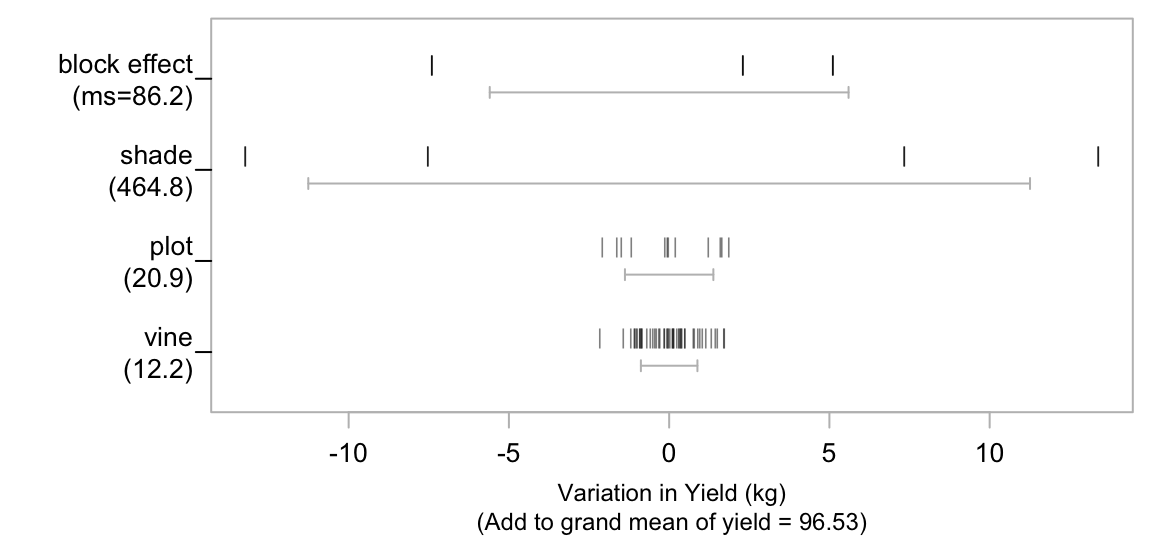
\includegraphics[width=0.8\textwidth,height=\textheight]{figs/g7_6-1.png}
\end{center}

\begin{Shaded}
\begin{Highlighting}[]
\NormalTok{kiwishade }\OtherTok{\textless{}{-}}\NormalTok{ DAAG}\SpecialCharTok{::}\NormalTok{kiwishade}
\NormalTok{kiwimeans }\OtherTok{\textless{}{-}} \FunctionTok{with}\NormalTok{(kiwishade, }\FunctionTok{aggregate}\NormalTok{(yield,}\AttributeTok{by=}\FunctionTok{list}\NormalTok{(block,shade),mean))}
\FunctionTok{names}\NormalTok{(kiwimeans) }\OtherTok{\textless{}{-}} \FunctionTok{c}\NormalTok{(}\StringTok{"block"}\NormalTok{,}\StringTok{"shade"}\NormalTok{,}\StringTok{"meanyield"}\NormalTok{)}
\NormalTok{plotmeans.lm }\OtherTok{\textless{}{-}} \FunctionTok{lm}\NormalTok{(meanyield}\SpecialCharTok{\textasciitilde{}}\NormalTok{block}\SpecialCharTok{+}\NormalTok{shade, }\AttributeTok{data=}\NormalTok{kiwimeans)}
\NormalTok{effects }\OtherTok{\textless{}{-}} \FunctionTok{predict}\NormalTok{(plotmeans.lm, }\AttributeTok{type=}\StringTok{"terms"}\NormalTok{)}
\NormalTok{kiwishade.lm }\OtherTok{\textless{}{-}} \FunctionTok{lm}\NormalTok{(yield }\SpecialCharTok{\textasciitilde{}}\NormalTok{ block}\SpecialCharTok{*}\NormalTok{shade, }\AttributeTok{data=}\NormalTok{kiwishade)}
\NormalTok{y }\OtherTok{\textless{}{-}} \FunctionTok{c}\NormalTok{(effects[,}\StringTok{"block"}\NormalTok{]}\SpecialCharTok{/}\FunctionTok{sqrt}\NormalTok{(}\DecValTok{2}\NormalTok{) }\SpecialCharTok{*} \FunctionTok{sqrt}\NormalTok{(}\DecValTok{16}\NormalTok{),}
\NormalTok{effects[,}\StringTok{"shade"}\NormalTok{]}\SpecialCharTok{/}\FunctionTok{sqrt}\NormalTok{(}\DecValTok{3}\NormalTok{) }\SpecialCharTok{*} \FunctionTok{sqrt}\NormalTok{(}\DecValTok{12}\NormalTok{),}
\FunctionTok{residuals}\NormalTok{(plotmeans.lm)}\SpecialCharTok{/}\FunctionTok{sqrt}\NormalTok{(}\DecValTok{6}\NormalTok{) }\SpecialCharTok{*} \FunctionTok{sqrt}\NormalTok{(}\DecValTok{4}\NormalTok{),}
\FunctionTok{residuals}\NormalTok{(kiwishade.lm)}\SpecialCharTok{/}\FunctionTok{sqrt}\NormalTok{(}\DecValTok{12}\NormalTok{))}
\NormalTok{n }\OtherTok{\textless{}{-}} \FunctionTok{rep}\NormalTok{(}\DecValTok{4}\SpecialCharTok{:}\DecValTok{1}\NormalTok{, }\FunctionTok{c}\NormalTok{(}\DecValTok{12}\NormalTok{, }\DecValTok{12}\NormalTok{, }\DecValTok{12}\NormalTok{, }\DecValTok{48}\NormalTok{))}
\NormalTok{gps }\OtherTok{\textless{}{-}} \FunctionTok{rep}\NormalTok{(}\FunctionTok{c}\NormalTok{(}\StringTok{"block effect}\SpecialCharTok{\textbackslash{}n}\StringTok{(ms=86.2)"}\NormalTok{, }\StringTok{"shade}\SpecialCharTok{\textbackslash{}n}\StringTok{(464.8)"}\NormalTok{,}
\StringTok{"plot}\SpecialCharTok{\textbackslash{}n}\StringTok{(20.9)"}\NormalTok{, }\StringTok{"vine}\SpecialCharTok{\textbackslash{}n}\StringTok{(12.2)"}\NormalTok{), }\FunctionTok{c}\NormalTok{(}\DecValTok{12}\NormalTok{, }\DecValTok{12}\NormalTok{, }\DecValTok{12}\NormalTok{, }\DecValTok{48}\NormalTok{))}
\NormalTok{gps }\OtherTok{\textless{}{-}} \FunctionTok{factor}\NormalTok{(gps, }\AttributeTok{levels =} \FunctionTok{rev}\NormalTok{(}\FunctionTok{c}\NormalTok{(}\StringTok{"block effect}\SpecialCharTok{\textbackslash{}n}\StringTok{(ms=86.2)"}\NormalTok{,}
\StringTok{"shade}\SpecialCharTok{\textbackslash{}n}\StringTok{(464.8)"}\NormalTok{, }\StringTok{"plot}\SpecialCharTok{\textbackslash{}n}\StringTok{(20.9)"}\NormalTok{, }\StringTok{"vine}\SpecialCharTok{\textbackslash{}n}\StringTok{(12.2)"}\NormalTok{)))}
\NormalTok{gps.sd }\OtherTok{\textless{}{-}} \FunctionTok{sapply}\NormalTok{(}\FunctionTok{split}\NormalTok{(y,gps), sd)}
\NormalTok{gps.av }\OtherTok{\textless{}{-}} \FunctionTok{sapply}\NormalTok{(}\FunctionTok{split}\NormalTok{(y,gps), mean)}
\FunctionTok{plot}\NormalTok{(}\FunctionTok{range}\NormalTok{(y), }\FunctionTok{range}\NormalTok{(n)}\SpecialCharTok{+}\FunctionTok{c}\NormalTok{(}\SpecialCharTok{{-}}\FloatTok{0.5}\NormalTok{, }\FloatTok{0.5}\NormalTok{), }\AttributeTok{xlab=}\StringTok{""}\NormalTok{, }\AttributeTok{ylab=}\StringTok{""}\NormalTok{, }\AttributeTok{yaxt=}\StringTok{"n"}\NormalTok{, }\AttributeTok{type=}\StringTok{"n"}\NormalTok{, }\AttributeTok{fg=}\StringTok{"gray"}\NormalTok{)}
\FunctionTok{text}\NormalTok{(y, n}\FloatTok{+0.15}\NormalTok{, }\StringTok{"|"}\NormalTok{, }\AttributeTok{cex=}\FloatTok{0.8}\NormalTok{, }\AttributeTok{col=}\FunctionTok{adjustcolor}\NormalTok{(}\StringTok{"black"}\NormalTok{, }\AttributeTok{alpha.f=}\FloatTok{0.5}\NormalTok{))}
\NormalTok{un }\OtherTok{\textless{}{-}} \DecValTok{1}\SpecialCharTok{:}\DecValTok{4}
\FunctionTok{sapply}\NormalTok{(un, }\ControlFlowTok{function}\NormalTok{(j)\{}\FunctionTok{lines}\NormalTok{(gps.av[j]}\SpecialCharTok{+}\FunctionTok{c}\NormalTok{(}\SpecialCharTok{{-}}\NormalTok{gps.sd[j], gps.sd[j]),}
\FunctionTok{rep}\NormalTok{(j}\FloatTok{{-}0.15}\NormalTok{,}\DecValTok{2}\NormalTok{), }\AttributeTok{col=}\StringTok{"gray"}\NormalTok{)}
\FunctionTok{lines}\NormalTok{(}\FunctionTok{rep}\NormalTok{(gps.av[j],}\DecValTok{2}\NormalTok{)}\SpecialCharTok{{-}}\NormalTok{gps.sd[j],}
\NormalTok{j}\FloatTok{{-}0.15}\SpecialCharTok{+}\FunctionTok{c}\NormalTok{(}\SpecialCharTok{{-}}\NormalTok{.}\DecValTok{06}\NormalTok{, .}\DecValTok{06}\NormalTok{), }\AttributeTok{col=}\StringTok{"gray"}\NormalTok{)}
\FunctionTok{lines}\NormalTok{(}\FunctionTok{rep}\NormalTok{(gps.av[j],}\DecValTok{2}\NormalTok{)}\SpecialCharTok{+}\NormalTok{gps.sd[j],}
\NormalTok{j}\FloatTok{{-}0.15}\SpecialCharTok{+}\FunctionTok{c}\NormalTok{(}\SpecialCharTok{{-}}\NormalTok{.}\DecValTok{06}\NormalTok{, .}\DecValTok{06}\NormalTok{), }\AttributeTok{col=}\StringTok{"gray"}\NormalTok{)}
\NormalTok{\})}
\FunctionTok{mtext}\NormalTok{(}\AttributeTok{side=}\DecValTok{1}\NormalTok{,}\AttributeTok{line=}\FloatTok{2.25}\NormalTok{, }\AttributeTok{cex=}\FloatTok{0.9}\NormalTok{,}
\AttributeTok{text=}\StringTok{"Variation in Yield (kg)}\SpecialCharTok{\textbackslash{}n}\StringTok{(Add to grand mean of yield = 96.53)"}\NormalTok{)}
\FunctionTok{par}\NormalTok{(}\AttributeTok{las=}\DecValTok{2}\NormalTok{)}
\FunctionTok{axis}\NormalTok{(}\DecValTok{2}\NormalTok{, }\AttributeTok{at=}\DecValTok{1}\SpecialCharTok{:}\DecValTok{4}\NormalTok{, }\AttributeTok{labels=}\FunctionTok{levels}\NormalTok{(gps), }\AttributeTok{lwd=}\DecValTok{0}\NormalTok{, }\AttributeTok{lwd.ticks=}\DecValTok{1}\NormalTok{)}
\end{Highlighting}
\end{Shaded}

\subsubsection{Subsection 7.4.4: The variance
components}\label{subsection-7.4.4-the-variance-components}

\subsubsection{Subsection 7.4.5: The mixed model
analysis}\label{subsection-7.4.5-the-mixed-model-analysis}

\begin{Shaded}
\begin{Highlighting}[]
\NormalTok{kiwishade.lmer }\OtherTok{\textless{}{-}} \FunctionTok{lmer}\NormalTok{(yield }\SpecialCharTok{\textasciitilde{}}\NormalTok{ shade }\SpecialCharTok{+}\NormalTok{ (}\DecValTok{1}\SpecialCharTok{|}\NormalTok{block) }\SpecialCharTok{+}\NormalTok{ (}\DecValTok{1}\SpecialCharTok{|}\NormalTok{block}\SpecialCharTok{:}\NormalTok{plot),}
\AttributeTok{data=}\NormalTok{kiwishade)}
\CommentTok{\# block:shade is an alternative to block:plot}
\end{Highlighting}
\end{Shaded}

\begin{Shaded}
\begin{Highlighting}[]
\FunctionTok{print}\NormalTok{(kiwishade.lmer, }\AttributeTok{ranef.comp=}\StringTok{"Variance"}\NormalTok{, }\AttributeTok{digits=}\DecValTok{3}\NormalTok{)}
\end{Highlighting}
\end{Shaded}

\begin{verbatim}
Linear mixed model fit by REML ['lmerMod']
Formula: yield ~ shade + (1 | block) + (1 | block:plot)
   Data: kiwishade
REML criterion at convergence: 252
Random effects:
 Groups     Name        Variance
 block:plot (Intercept)  2.19   
 block      (Intercept)  4.08   
 Residual               12.18   
Number of obs: 48, groups:  block:plot, 12; block, 3
Fixed Effects:
 (Intercept)  shadeAug2Dec  shadeDec2Feb  shadeFeb2May  
      100.20          3.03        -10.28         -7.43  
\end{verbatim}

\paragraph{Residuals and estimated
effects}\label{residuals-and-estimated-effects}

\begin{center}
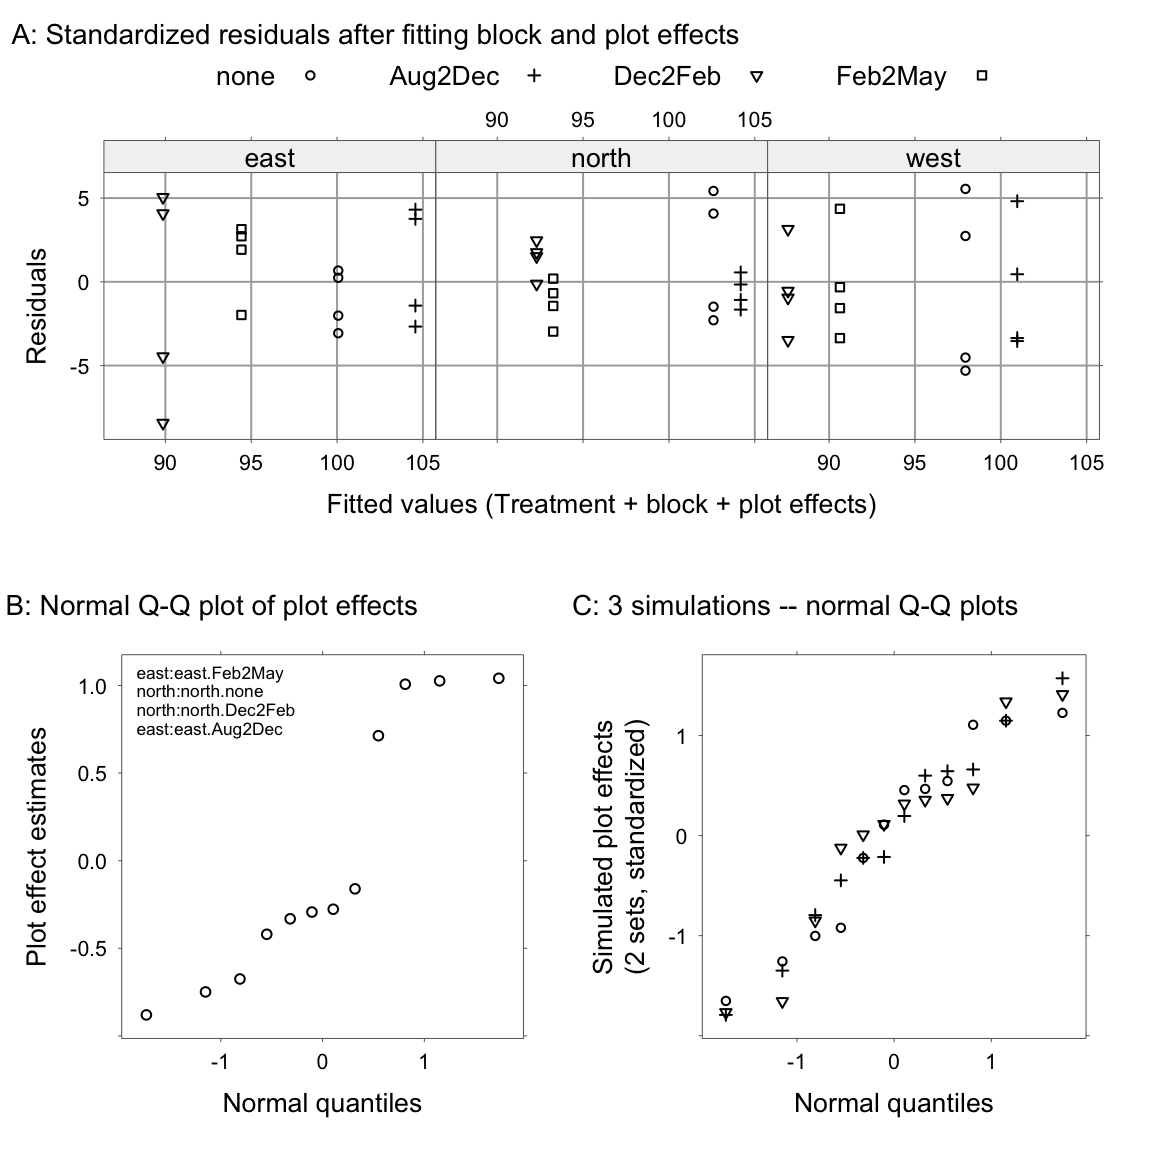
\includegraphics[width=1\textwidth,height=\textheight]{figs/g7_7-1.png}
\end{center}

\begin{Shaded}
\begin{Highlighting}[]
\DocumentationTok{\#\# Panel A}
\NormalTok{parsetA }\OtherTok{\textless{}{-}} \FunctionTok{modifyList}\NormalTok{(DAAG}\SpecialCharTok{::}\FunctionTok{DAAGtheme}\NormalTok{(}\AttributeTok{color=}\ConstantTok{FALSE}\NormalTok{),}
                      \FunctionTok{list}\NormalTok{(}\AttributeTok{layout.heights=}\FunctionTok{list}\NormalTok{(}\AttributeTok{key.top=}\FloatTok{2.25}\NormalTok{, }\AttributeTok{axis.top=}\NormalTok{.}\DecValTok{75}\NormalTok{)))}
\ControlFlowTok{if}\NormalTok{ (}\SpecialCharTok{!}\FunctionTok{exists}\NormalTok{(}\StringTok{"kiwishade.lmer"}\NormalTok{))}
\NormalTok{kiwishade.lmer }\OtherTok{\textless{}{-}}\NormalTok{ lme4}\SpecialCharTok{::}\FunctionTok{lmer}\NormalTok{(yield }\SpecialCharTok{\textasciitilde{}}\NormalTok{ shade }\SpecialCharTok{+}\NormalTok{ (}\DecValTok{1}\SpecialCharTok{|}\NormalTok{block}\SpecialCharTok{/}\NormalTok{shade), }\AttributeTok{data=}\NormalTok{kiwishade)}
\NormalTok{pk1 }\OtherTok{\textless{}{-}} \FunctionTok{xyplot}\NormalTok{(}\FunctionTok{residuals}\NormalTok{(kiwishade.lmer) }\SpecialCharTok{\textasciitilde{}} \FunctionTok{fitted}\NormalTok{(kiwishade.lmer)}\SpecialCharTok{|}\NormalTok{block,}
              \AttributeTok{groups=}\NormalTok{shade, }\AttributeTok{layout=}\FunctionTok{c}\NormalTok{(}\DecValTok{3}\NormalTok{,}\DecValTok{1}\NormalTok{), }\AttributeTok{par.strip.text=}\FunctionTok{list}\NormalTok{(}\AttributeTok{cex=}\FloatTok{1.0}\NormalTok{),}
              \AttributeTok{data=}\NormalTok{kiwishade, }\AttributeTok{grid=}\ConstantTok{TRUE}\NormalTok{,}
              \AttributeTok{xlab=}\StringTok{"Fitted values (Treatment + block + plot effects)"}\NormalTok{,}
              \AttributeTok{ylab=}\StringTok{"Residuals"}\NormalTok{,}
  \AttributeTok{main=}\FunctionTok{list}\NormalTok{(}\AttributeTok{label=}\StringTok{"A: Standardized residuals after fitting block and plot effects"}\NormalTok{,}
          \AttributeTok{cex=}\FloatTok{1.05}\NormalTok{, }\AttributeTok{x=}\FloatTok{0.01}\NormalTok{, }\AttributeTok{y=}\DecValTok{0}\NormalTok{, }\AttributeTok{font=}\DecValTok{1}\NormalTok{, }\AttributeTok{just=}\StringTok{"left"}\NormalTok{),}
             \AttributeTok{auto.key=}\FunctionTok{list}\NormalTok{(}\AttributeTok{space=}\StringTok{\textquotesingle{}top\textquotesingle{}}\NormalTok{, }\AttributeTok{points=}\ConstantTok{TRUE}\NormalTok{, }\AttributeTok{columns=}\DecValTok{4}\NormalTok{))}
\FunctionTok{print}\NormalTok{(}\FunctionTok{update}\NormalTok{(pk1, }\AttributeTok{scales=}\FunctionTok{list}\NormalTok{(}\AttributeTok{x=}\FunctionTok{list}\NormalTok{(}\AttributeTok{alternating=}\ConstantTok{TRUE}\NormalTok{), }\AttributeTok{tck=}\FloatTok{0.35}\NormalTok{),}
             \AttributeTok{par.settings=}\NormalTok{parsetA), }\AttributeTok{position=}\FunctionTok{c}\NormalTok{(}\DecValTok{0}\NormalTok{,.}\DecValTok{52}\NormalTok{,}\DecValTok{1}\NormalTok{,}\DecValTok{1}\NormalTok{))}
\DocumentationTok{\#\# Panel B}
\NormalTok{ploteff }\OtherTok{\textless{}{-}} \FunctionTok{ranef}\NormalTok{(kiwishade.lmer, }\AttributeTok{drop=}\ConstantTok{TRUE}\NormalTok{)[[}\DecValTok{1}\NormalTok{]]}
\NormalTok{nam }\OtherTok{\textless{}{-}} \FunctionTok{names}\NormalTok{(}\FunctionTok{sort}\NormalTok{(ploteff, }\AttributeTok{decreasing=}\ConstantTok{TRUE}\NormalTok{)[}\DecValTok{1}\SpecialCharTok{:}\DecValTok{4}\NormalTok{])}
\NormalTok{parsetB }\OtherTok{\textless{}{-}} \FunctionTok{modifyList}\NormalTok{(DAAG}\SpecialCharTok{::}\FunctionTok{DAAGtheme}\NormalTok{(}\AttributeTok{color=}\ConstantTok{FALSE}\NormalTok{),}
                      \FunctionTok{list}\NormalTok{(}\AttributeTok{layout.heights=}\FunctionTok{list}\NormalTok{(}\AttributeTok{axis.top=}\FloatTok{0.85}\NormalTok{)))}
\NormalTok{pk2 }\OtherTok{\textless{}{-}} \FunctionTok{qqmath}\NormalTok{(ploteff, }\AttributeTok{ylab=}\StringTok{"Plot effect estimates"}\NormalTok{,}
              \AttributeTok{key=}\FunctionTok{list}\NormalTok{(}\AttributeTok{x=}\DecValTok{0}\NormalTok{, }\AttributeTok{y=}\FloatTok{0.98}\NormalTok{, }\AttributeTok{corner=}\FunctionTok{c}\NormalTok{(}\DecValTok{0}\NormalTok{,}\DecValTok{1}\NormalTok{),}
              \AttributeTok{text=}\FunctionTok{list}\NormalTok{(}\AttributeTok{labels=}\NormalTok{nam, }\AttributeTok{cex=}\FloatTok{0.65}\NormalTok{)),}
              \AttributeTok{main=}\FunctionTok{list}\NormalTok{(}\AttributeTok{label=}\StringTok{"B: Normal Q{-}Q plot of plot effects"}\NormalTok{,}
                        \AttributeTok{cex=}\FloatTok{1.05}\NormalTok{, }\AttributeTok{x=}\FloatTok{0.01}\NormalTok{, }\AttributeTok{y=}\FloatTok{0.25}\NormalTok{, }\AttributeTok{font=}\DecValTok{1}\NormalTok{, }\AttributeTok{just=}\StringTok{"left"}\NormalTok{),}
              \AttributeTok{xlab=}\StringTok{"Normal quantiles"}\NormalTok{)}
\FunctionTok{print}\NormalTok{(}\FunctionTok{update}\NormalTok{(pk2, }\AttributeTok{scales=}\FunctionTok{list}\NormalTok{(}\AttributeTok{tck=}\FloatTok{0.35}\NormalTok{), }\AttributeTok{par.settings=}\NormalTok{parsetB),}
      \AttributeTok{newpage=}\ConstantTok{FALSE}\NormalTok{, }\AttributeTok{position=}\FunctionTok{c}\NormalTok{(}\DecValTok{0}\NormalTok{,}\DecValTok{0}\NormalTok{,.}\DecValTok{5}\NormalTok{,.}\DecValTok{5}\NormalTok{))}
\DocumentationTok{\#\# Panel C}
\NormalTok{simvals }\OtherTok{\textless{}{-}} \FunctionTok{simulate}\NormalTok{(kiwishade.lmer, }\AttributeTok{nsim=}\DecValTok{3}\NormalTok{, }\AttributeTok{seed=}\DecValTok{23}\NormalTok{)}
\NormalTok{simranef }\OtherTok{\textless{}{-}} \ControlFlowTok{function}\NormalTok{(y)}\FunctionTok{ranef}\NormalTok{(lme4}\SpecialCharTok{::}\FunctionTok{refit}\NormalTok{(kiwishade.lmer, y))[[}\DecValTok{1}\NormalTok{]]}
\NormalTok{simeff }\OtherTok{\textless{}{-}} \FunctionTok{apply}\NormalTok{(simvals, }\DecValTok{2}\NormalTok{, }\ControlFlowTok{function}\NormalTok{(y) }\FunctionTok{scale}\NormalTok{(}\FunctionTok{simranef}\NormalTok{(y)))}
\NormalTok{simeff }\OtherTok{\textless{}{-}} \FunctionTok{as.data.frame}\NormalTok{(simeff)}
\NormalTok{pk3 }\OtherTok{\textless{}{-}} \FunctionTok{qqmath}\NormalTok{(}\SpecialCharTok{\textasciitilde{}}\NormalTok{ sim\_1}\SpecialCharTok{+}\NormalTok{sim\_2}\SpecialCharTok{+}\NormalTok{sim\_3, }\AttributeTok{data=}\NormalTok{simeff,}
              \AttributeTok{ylab=}\StringTok{"Simulated plot effects}\SpecialCharTok{\textbackslash{}n}\StringTok{(2 sets, standardized)"}\NormalTok{,}
              \AttributeTok{Qs=}\FunctionTok{list}\NormalTok{(}\AttributeTok{tck=}\FloatTok{0.35}\NormalTok{), }\AttributeTok{aspect=}\DecValTok{1}\NormalTok{,}
               \AttributeTok{main=}\FunctionTok{list}\NormalTok{(}\AttributeTok{label=}\StringTok{"C: 3 simulations {-}{-} normal Q{-}Q plots"}\NormalTok{,}
                         \AttributeTok{x=}\FloatTok{0.01}\NormalTok{, }\AttributeTok{y=}\FloatTok{0.25}\NormalTok{, }\AttributeTok{cex=}\FloatTok{1.05}\NormalTok{, }\AttributeTok{font=}\DecValTok{1}\NormalTok{, }\AttributeTok{just=}\StringTok{"left"}\NormalTok{),}
               \AttributeTok{xlab=}\StringTok{"Normal quantiles"}\NormalTok{)}
\FunctionTok{print}\NormalTok{(}\FunctionTok{update}\NormalTok{(pk3, }\AttributeTok{scales=}\FunctionTok{list}\NormalTok{(}\AttributeTok{tck=}\FloatTok{0.35}\NormalTok{), }\AttributeTok{par.settings=}\NormalTok{parsetB),}
      \AttributeTok{newpage=}\ConstantTok{FALSE}\NormalTok{, }\AttributeTok{position=}\FunctionTok{c}\NormalTok{(}\FloatTok{0.48}\NormalTok{,}\DecValTok{0}\NormalTok{,}\DecValTok{1}\NormalTok{,.}\DecValTok{5}\NormalTok{))}
\end{Highlighting}
\end{Shaded}

\begin{Shaded}
\begin{Highlighting}[]
\FunctionTok{with}\NormalTok{(kiwishade, }\FunctionTok{sapply}\NormalTok{(}\FunctionTok{split}\NormalTok{(yield, shade), mean))}
\end{Highlighting}
\end{Shaded}

\begin{verbatim}
   none Aug2Dec Dec2Feb Feb2May 
 100.20  103.23   89.92   92.77 
\end{verbatim}

\subsubsection{Subsection 7.4.6: Predictive
accuracy}\label{subsection-7.4.6-predictive-accuracy}

\subsection{Section 7.5 Within and between subject
effects}\label{section-7.5-within-and-between-subject-effects}

\begin{center}
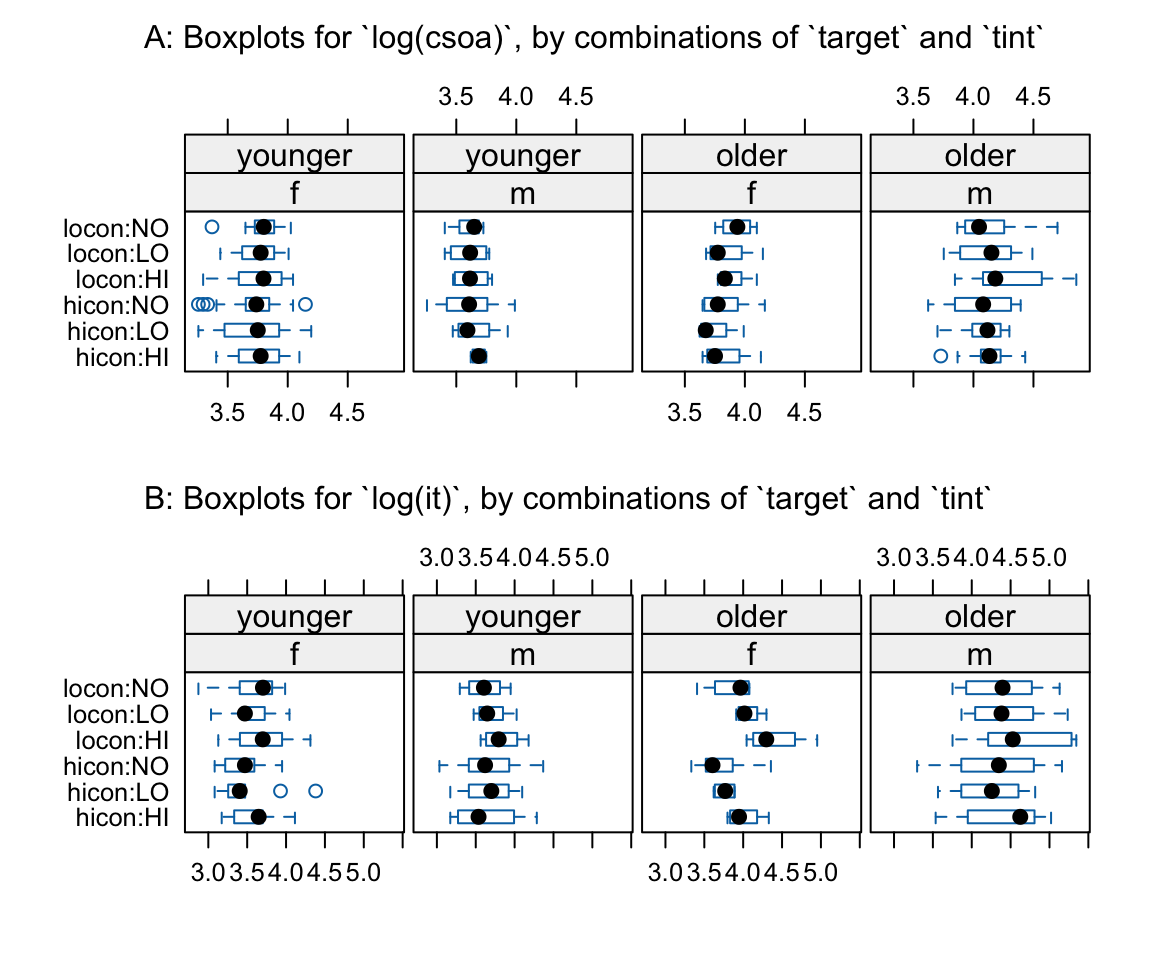
\includegraphics[width=1\textwidth,height=\textheight]{figs/g7_8-1.png}
\end{center}

\begin{Shaded}
\begin{Highlighting}[]
\FunctionTok{library}\NormalTok{(lattice)}
\NormalTok{tinting }\OtherTok{\textless{}{-}} \FunctionTok{within}\NormalTok{(DAAG}\SpecialCharTok{::}\NormalTok{tinting, targtint }\OtherTok{\textless{}{-}} \FunctionTok{paste}\NormalTok{(target,}\FunctionTok{toupper}\NormalTok{(tint),}\AttributeTok{sep=}\StringTok{\textquotesingle{}:\textquotesingle{}}\NormalTok{))}
\NormalTok{gphA }\OtherTok{\textless{}{-}} \FunctionTok{bwplot}\NormalTok{(targtint}\SpecialCharTok{\textasciitilde{}}\FunctionTok{log}\NormalTok{(csoa) }\SpecialCharTok{|}\NormalTok{ sex}\SpecialCharTok{*}\NormalTok{agegp, }\AttributeTok{data=}\NormalTok{tinting, }\AttributeTok{layout=}\FunctionTok{c}\NormalTok{(}\DecValTok{4}\NormalTok{,}\DecValTok{1}\NormalTok{), }\AttributeTok{between=}\FunctionTok{list}\NormalTok{(}\AttributeTok{x=}\FloatTok{0.25}\NormalTok{))}
\NormalTok{mainA }\OtherTok{\textless{}{-}} \FunctionTok{list}\NormalTok{(}\StringTok{"A: Boxplots for \textasciigrave{}log(csoa)\textasciigrave{}, by combinations of \textasciigrave{}target\textasciigrave{} and \textasciigrave{}tint\textasciigrave{}"}\NormalTok{,}
              \AttributeTok{font=}\DecValTok{1}\NormalTok{, }\AttributeTok{x=}\FloatTok{0.125}\NormalTok{, }\AttributeTok{y=}\FloatTok{0.125}\NormalTok{, }\AttributeTok{cex=}\FloatTok{1.0}\NormalTok{, }\AttributeTok{just=}\StringTok{\textquotesingle{}left\textquotesingle{}}\NormalTok{)}
\NormalTok{gphB }\OtherTok{\textless{}{-}} \FunctionTok{bwplot}\NormalTok{(targtint}\SpecialCharTok{\textasciitilde{}}\FunctionTok{log}\NormalTok{(it) }\SpecialCharTok{|}\NormalTok{ sex}\SpecialCharTok{*}\NormalTok{agegp, }\AttributeTok{data=}\NormalTok{tinting, }\AttributeTok{layout=}\FunctionTok{c}\NormalTok{(}\DecValTok{4}\NormalTok{,}\DecValTok{1}\NormalTok{), }\AttributeTok{between=}\FunctionTok{list}\NormalTok{(}\AttributeTok{x=}\FloatTok{0.25}\NormalTok{))}
\NormalTok{mainB }\OtherTok{\textless{}{-}} \FunctionTok{list}\NormalTok{(}\StringTok{"B: Boxplots for \textasciigrave{}log(it)\textasciigrave{}, by combinations of \textasciigrave{}target\textasciigrave{} and \textasciigrave{}tint\textasciigrave{}"}\NormalTok{,}
              \AttributeTok{font=}\DecValTok{1}\NormalTok{, }\AttributeTok{x=}\FloatTok{0.125}\NormalTok{, }\AttributeTok{y=}\FloatTok{0.125}\NormalTok{, }\AttributeTok{cex=}\FloatTok{1.0}\NormalTok{, }\AttributeTok{just=}\StringTok{\textquotesingle{}left\textquotesingle{}}\NormalTok{)}
\FunctionTok{print}\NormalTok{(}\FunctionTok{update}\NormalTok{(gphA, }\AttributeTok{main=}\NormalTok{mainA, }\AttributeTok{xlab=}\StringTok{""}\NormalTok{), }\AttributeTok{position=}\FunctionTok{c}\NormalTok{(}\DecValTok{0}\NormalTok{, }\FloatTok{0.48}\NormalTok{, }\DecValTok{1}\NormalTok{, }\FloatTok{1.0}\NormalTok{), }\AttributeTok{more=}\NormalTok{T)}
\FunctionTok{print}\NormalTok{(}\FunctionTok{update}\NormalTok{(gphB, }\AttributeTok{main=}\NormalTok{mainB, }\AttributeTok{xlab=}\StringTok{""}\NormalTok{), }\AttributeTok{position=}\FunctionTok{c}\NormalTok{(}\DecValTok{0}\NormalTok{,}\DecValTok{0}\NormalTok{,}\DecValTok{1}\NormalTok{,}\FloatTok{0.52}\NormalTok{))}
\end{Highlighting}
\end{Shaded}

\paragraph{Model fitting criteria}\label{model-fitting-criteria}

\subsubsection{Subsection 7.5.1: Model
selection}\label{subsection-7.5.1-model-selection}

\begin{Shaded}
\begin{Highlighting}[]
\DocumentationTok{\#\# Capitalize tinting$agegp}
\FunctionTok{levels}\NormalTok{(tinting}\SpecialCharTok{$}\NormalTok{agegp) }\OtherTok{\textless{}{-}}\NormalTok{ R.utils}\SpecialCharTok{::}\FunctionTok{capitalize}\NormalTok{(}\FunctionTok{levels}\NormalTok{(tinting}\SpecialCharTok{$}\NormalTok{agegp))}
\DocumentationTok{\#\# Fit all interactions: data frame tinting (DAAG)}
\NormalTok{it3.lmer }\OtherTok{\textless{}{-}} \FunctionTok{lmer}\NormalTok{(}\FunctionTok{log}\NormalTok{(it) }\SpecialCharTok{\textasciitilde{}}\NormalTok{ tint}\SpecialCharTok{*}\NormalTok{target}\SpecialCharTok{*}\NormalTok{agegp}\SpecialCharTok{*}\NormalTok{sex }\SpecialCharTok{+}\NormalTok{ (}\DecValTok{1} \SpecialCharTok{|}\NormalTok{ id),}
                 \AttributeTok{data=}\NormalTok{DAAG}\SpecialCharTok{::}\NormalTok{tinting, }\AttributeTok{REML=}\ConstantTok{FALSE}\NormalTok{)}
\end{Highlighting}
\end{Shaded}

\begin{Shaded}
\begin{Highlighting}[]
\NormalTok{it2.lmer }\OtherTok{\textless{}{-}} \FunctionTok{lmer}\NormalTok{(}\FunctionTok{log}\NormalTok{(it) }\SpecialCharTok{\textasciitilde{}}\NormalTok{ (tint}\SpecialCharTok{+}\NormalTok{target}\SpecialCharTok{+}\NormalTok{agegp}\SpecialCharTok{+}\NormalTok{sex)}\SpecialCharTok{\^{}}\DecValTok{2} \SpecialCharTok{+}\NormalTok{ (}\DecValTok{1} \SpecialCharTok{|}\NormalTok{ id),}
                 \AttributeTok{data=}\NormalTok{DAAG}\SpecialCharTok{::}\NormalTok{tinting, }\AttributeTok{REML=}\ConstantTok{FALSE}\NormalTok{)}
\end{Highlighting}
\end{Shaded}

\begin{Shaded}
\begin{Highlighting}[]
\NormalTok{it1.lmer }\OtherTok{\textless{}{-}} \FunctionTok{lmer}\NormalTok{(}\FunctionTok{log}\NormalTok{(it)}\SpecialCharTok{\textasciitilde{}}\NormalTok{(tint}\SpecialCharTok{+}\NormalTok{target}\SpecialCharTok{+}\NormalTok{agegp}\SpecialCharTok{+}\NormalTok{sex) }\SpecialCharTok{+}\NormalTok{ (}\DecValTok{1} \SpecialCharTok{|}\NormalTok{ id),}
                 \AttributeTok{data=}\NormalTok{DAAG}\SpecialCharTok{::}\NormalTok{tinting, }\AttributeTok{REML=}\ConstantTok{FALSE}\NormalTok{)}
\end{Highlighting}
\end{Shaded}

\begin{Shaded}
\begin{Highlighting}[]
\FunctionTok{anova}\NormalTok{(it1.lmer, it2.lmer, it3.lmer)}
\end{Highlighting}
\end{Shaded}

\begin{verbatim}
Data: DAAG::tinting
Models:
it1.lmer: log(it) ~ (tint + target + agegp + sex) + (1 | id)
it2.lmer: log(it) ~ (tint + target + agegp + sex)^2 + (1 | id)
it3.lmer: log(it) ~ tint * target * agegp * sex + (1 | id)
         npar   AIC  BIC logLik deviance Chisq Df Pr(>Chisq)
it1.lmer    8  1.14 26.8   7.43    -14.9                    
it2.lmer   17 -3.74 50.7  18.87    -37.7 22.88  9     0.0065
it3.lmer   26  8.15 91.5  21.93    -43.9  6.11  9     0.7288
\end{verbatim}

\begin{Shaded}
\begin{Highlighting}[]
\DocumentationTok{\#\# Code that gives the first four such plots, for the observed data}
\FunctionTok{interaction.plot}\NormalTok{(tinting}\SpecialCharTok{$}\NormalTok{tint, tinting}\SpecialCharTok{$}\NormalTok{agegp, }\FunctionTok{log}\NormalTok{(tinting}\SpecialCharTok{$}\NormalTok{it))}
\FunctionTok{interaction.plot}\NormalTok{(tinting}\SpecialCharTok{$}\NormalTok{target, tinting}\SpecialCharTok{$}\NormalTok{sex, }\FunctionTok{log}\NormalTok{(tinting}\SpecialCharTok{$}\NormalTok{it))}
\FunctionTok{interaction.plot}\NormalTok{(tinting}\SpecialCharTok{$}\NormalTok{tint, tinting}\SpecialCharTok{$}\NormalTok{target, }\FunctionTok{log}\NormalTok{(tinting}\SpecialCharTok{$}\NormalTok{it))}
\FunctionTok{interaction.plot}\NormalTok{(tinting}\SpecialCharTok{$}\NormalTok{tint, tinting}\SpecialCharTok{$}\NormalTok{sex, }\FunctionTok{log}\NormalTok{(tinting}\SpecialCharTok{$}\NormalTok{it))}
\end{Highlighting}
\end{Shaded}

\subsubsection{Subsection 7.5.2: Estimates of model
parameters}\label{subsection-7.5.2-estimates-of-model-parameters}

\begin{Shaded}
\begin{Highlighting}[]
\NormalTok{it2.reml }\OtherTok{\textless{}{-}} \FunctionTok{update}\NormalTok{(it2.lmer, }\AttributeTok{REML=}\ConstantTok{TRUE}\NormalTok{)}
\FunctionTok{print}\NormalTok{(}\FunctionTok{coef}\NormalTok{(}\FunctionTok{summary}\NormalTok{(it2.reml)), }\AttributeTok{digits=}\DecValTok{2}\NormalTok{)}
\end{Highlighting}
\end{Shaded}

\begin{verbatim}
                       Estimate Std. Error t value
(Intercept)              3.6191      0.130   27.82
tint.L                   0.1609      0.044    3.64
tint.Q                   0.0210      0.045    0.46
targethicon             -0.1181      0.042   -2.79
agegpolder               0.4712      0.233    2.02
sexm                     0.0821      0.233    0.35
tint.L:targethicon      -0.0919      0.046   -2.00
tint.Q:targethicon      -0.0072      0.048   -0.15
tint.L:agegpolder        0.1308      0.049    2.66
tint.Q:agegpolder        0.0697      0.052    1.34
tint.L:sexm             -0.0979      0.049   -1.99
tint.Q:sexm              0.0054      0.052    0.10
targethicon:agegpolder  -0.1389      0.058   -2.38
targethicon:sexm         0.0779      0.058    1.33
agegpolder:sexm          0.3316      0.326    1.02
\end{verbatim}

\begin{Shaded}
\begin{Highlighting}[]
\CommentTok{\# NB: The final column, giving degrees of freedom, is not in the}
\CommentTok{\# summary output. It is our addition.}
\end{Highlighting}
\end{Shaded}

\begin{Shaded}
\begin{Highlighting}[]
\NormalTok{subs }\OtherTok{\textless{}{-}} \FunctionTok{with}\NormalTok{(tinting, }\FunctionTok{match}\NormalTok{(}\FunctionTok{unique}\NormalTok{(id), id))}
\FunctionTok{with}\NormalTok{(tinting, }\FunctionTok{table}\NormalTok{(sex[subs], agegp[subs]))}
\end{Highlighting}
\end{Shaded}

\begin{verbatim}
   
    Younger Older
  f       9     4
  m       4     9
\end{verbatim}

\subsection{Section 7.6 A mixed model with a betabinomial
error}\label{section-7.6-a-mixed-model-with-a-betabinomial-error}

\subsubsection{Subsection 7.6.1: The betabinomial
distribution}\label{subsection-7.6.1-the-betabinomial-distribution}

\begin{Shaded}
\begin{Highlighting}[]
\DocumentationTok{\#\# devtools::install\_github("jhmaindonald/qra")  \# Use if not found on CRAN}
\end{Highlighting}
\end{Shaded}

\paragraph{Notation}\label{notation}

\paragraph{Source of data}\label{source-of-data}

\begin{Shaded}
\begin{Highlighting}[]
\NormalTok{HawCon }\OtherTok{\textless{}{-}} \FunctionTok{within}\NormalTok{(}\FunctionTok{as.data.frame}\NormalTok{(qra}\SpecialCharTok{::}\NormalTok{HawCon), \{}
\NormalTok{  trtGp }\OtherTok{\textless{}{-}} \FunctionTok{gsub}\NormalTok{(}\StringTok{"Fly"}\NormalTok{, }\StringTok{""}\NormalTok{, }\FunctionTok{paste0}\NormalTok{(CN,LifestageTrt))}
\NormalTok{  trtGp }\OtherTok{\textless{}{-}} \FunctionTok{factor}\NormalTok{(trtGp, }\AttributeTok{levels=}\FunctionTok{sort}\NormalTok{(}\FunctionTok{unique}\NormalTok{(trtGp))[}\FunctionTok{c}\NormalTok{(}\DecValTok{1}\NormalTok{,}\DecValTok{5}\NormalTok{,}\DecValTok{2}\NormalTok{,}\DecValTok{6}\NormalTok{,}\DecValTok{3}\NormalTok{,}\DecValTok{7}\NormalTok{,}\DecValTok{4}\NormalTok{,}\DecValTok{8}\NormalTok{)])}
\NormalTok{  trtGpRep }\OtherTok{\textless{}{-}} \FunctionTok{paste0}\NormalTok{(CN,LifestageTrt,}\StringTok{":"}\NormalTok{,RepNumber)}
\NormalTok{  scTime }\OtherTok{\textless{}{-}} \FunctionTok{scale}\NormalTok{(TrtTime)  }\CommentTok{\# Centering and scaling can help model fit}
\NormalTok{  \})}
\end{Highlighting}
\end{Shaded}

\begin{Shaded}
\begin{Highlighting}[]
\DocumentationTok{\#\# Load packages that will be used}
\FunctionTok{suppressMessages}\NormalTok{(}\FunctionTok{library}\NormalTok{(lme4)); }\FunctionTok{suppressMessages}\NormalTok{(}\FunctionTok{library}\NormalTok{(glmmTMB))}
\end{Highlighting}
\end{Shaded}

\begin{Shaded}
\begin{Highlighting}[]
\FunctionTok{library}\NormalTok{(splines)}
\NormalTok{form }\OtherTok{\textless{}{-}} \FunctionTok{cbind}\NormalTok{(Dead,Live)}\SpecialCharTok{\textasciitilde{}}\DecValTok{0}\SpecialCharTok{+}\NormalTok{trtGp}\SpecialCharTok{/}\NormalTok{TrtTime}\SpecialCharTok{+}\NormalTok{(}\DecValTok{1}\SpecialCharTok{|}\NormalTok{trtGpRep)}
\DocumentationTok{\#\# Add the quadratic term from a degree 2 orthogonal polynomial}
\NormalTok{form2s }\OtherTok{\textless{}{-}} \FunctionTok{update}\NormalTok{(form, . }\SpecialCharTok{\textasciitilde{}}\NormalTok{ . }\SpecialCharTok{+} \FunctionTok{scale}\NormalTok{(scTime}\SpecialCharTok{\^{}}\DecValTok{2}\NormalTok{))}
  \DocumentationTok{\#\# Scale "corrections" to reduce risk of potential numerical problems}
\NormalTok{HCbb.cll }\OtherTok{\textless{}{-}} \FunctionTok{glmmTMB}\NormalTok{(form, }\AttributeTok{dispformula=}\SpecialCharTok{\textasciitilde{}}\NormalTok{trtGp}\SpecialCharTok{+}\FunctionTok{ns}\NormalTok{(scTime,}\DecValTok{2}\NormalTok{),}
                    \AttributeTok{family=}\NormalTok{glmmTMB}\SpecialCharTok{::}\FunctionTok{betabinomial}\NormalTok{(}\AttributeTok{link=}\StringTok{"cloglog"}\NormalTok{), }\AttributeTok{data=}\NormalTok{HawCon)}
\NormalTok{HCbb2s.cll }\OtherTok{\textless{}{-}} \FunctionTok{update}\NormalTok{(HCbb.cll, }\AttributeTok{formula=}\NormalTok{form2s)}
\NormalTok{HCbb.logit }\OtherTok{\textless{}{-}} \FunctionTok{glmmTMB}\NormalTok{(form, }\AttributeTok{dispformula=}\SpecialCharTok{\textasciitilde{}}\NormalTok{trtGp}\SpecialCharTok{+}\FunctionTok{ns}\NormalTok{(scTime,}\DecValTok{2}\NormalTok{),}
                      \AttributeTok{family=}\NormalTok{glmmTMB}\SpecialCharTok{::}\FunctionTok{betabinomial}\NormalTok{(}\AttributeTok{link=}\StringTok{"logit"}\NormalTok{), }\AttributeTok{data=}\NormalTok{HawCon)}
\NormalTok{HCbb2s.logit }\OtherTok{\textless{}{-}} \FunctionTok{update}\NormalTok{(HCbb.logit, }\AttributeTok{formula=}\NormalTok{form2s)}
\end{Highlighting}
\end{Shaded}

\begin{Shaded}
\begin{Highlighting}[]
\FunctionTok{summary}\NormalTok{(HCbb2s.cll)}\SpecialCharTok{$}\NormalTok{coefficients}\SpecialCharTok{$}\NormalTok{cond[}\StringTok{"scale(scTime\^{}2)"}\NormalTok{,]    }\DocumentationTok{\#\# CLL}
\end{Highlighting}
\end{Shaded}

\begin{verbatim}
  Estimate Std. Error    z value   Pr(>|z|) 
  -0.09130    0.06143   -1.48627    0.13721 
\end{verbatim}

\begin{Shaded}
\begin{Highlighting}[]
\FunctionTok{summary}\NormalTok{(HCbb2s.logit)}\SpecialCharTok{$}\NormalTok{coefficients}\SpecialCharTok{$}\NormalTok{cond[}\StringTok{"scale(scTime\^{}2)"}\NormalTok{,]  }\DocumentationTok{\#\# Logit}
\end{Highlighting}
\end{Shaded}

\begin{verbatim}
  Estimate Std. Error    z value   Pr(>|z|) 
   0.43219    0.17766    2.43268    0.01499 
\end{verbatim}

\begin{Shaded}
\begin{Highlighting}[]
\NormalTok{AICtab }\OtherTok{\textless{}{-}} \FunctionTok{AIC}\NormalTok{(}\AttributeTok{BB=}\NormalTok{HCbb.cll,HCbb2s.cll,HCbb.logit,HCbb2s.logit)}
\NormalTok{AICtab[[}\StringTok{\textquotesingle{}Details\textquotesingle{}}\NormalTok{]] }\OtherTok{\textless{}{-}} \FunctionTok{c}\NormalTok{(}\FunctionTok{paste0}\NormalTok{(}\StringTok{\textquotesingle{}BB: Compl. log{-}log\textquotesingle{}}\NormalTok{, }\FunctionTok{c}\NormalTok{(}\StringTok{\textquotesingle{}\textquotesingle{}}\NormalTok{, }\StringTok{\textquotesingle{}, added curve\textquotesingle{}}\NormalTok{)),}
                          \FunctionTok{paste0}\NormalTok{(}\StringTok{\textquotesingle{}BB: Logit\textquotesingle{}}\NormalTok{, }\FunctionTok{c}\NormalTok{(}\StringTok{\textquotesingle{}\textquotesingle{}}\NormalTok{, }\StringTok{\textquotesingle{}, added curve\textquotesingle{}}\NormalTok{)))}
\NormalTok{AICtab[}\FunctionTok{order}\NormalTok{(AICtab[[}\StringTok{"AIC"}\NormalTok{]]), ]}
\end{Highlighting}
\end{Shaded}

\begin{verbatim}
             df   AIC                         Details
HCbb2s.cll   28 709.9              BB: Compl. log-log
HCbb.cll     27 710.0 BB: Compl. log-log, added curve
HCbb2s.logit 28 717.2          BB: Logit, added curve
HCbb.logit   27 721.7                       BB: Logit
\end{verbatim}

\begin{center}
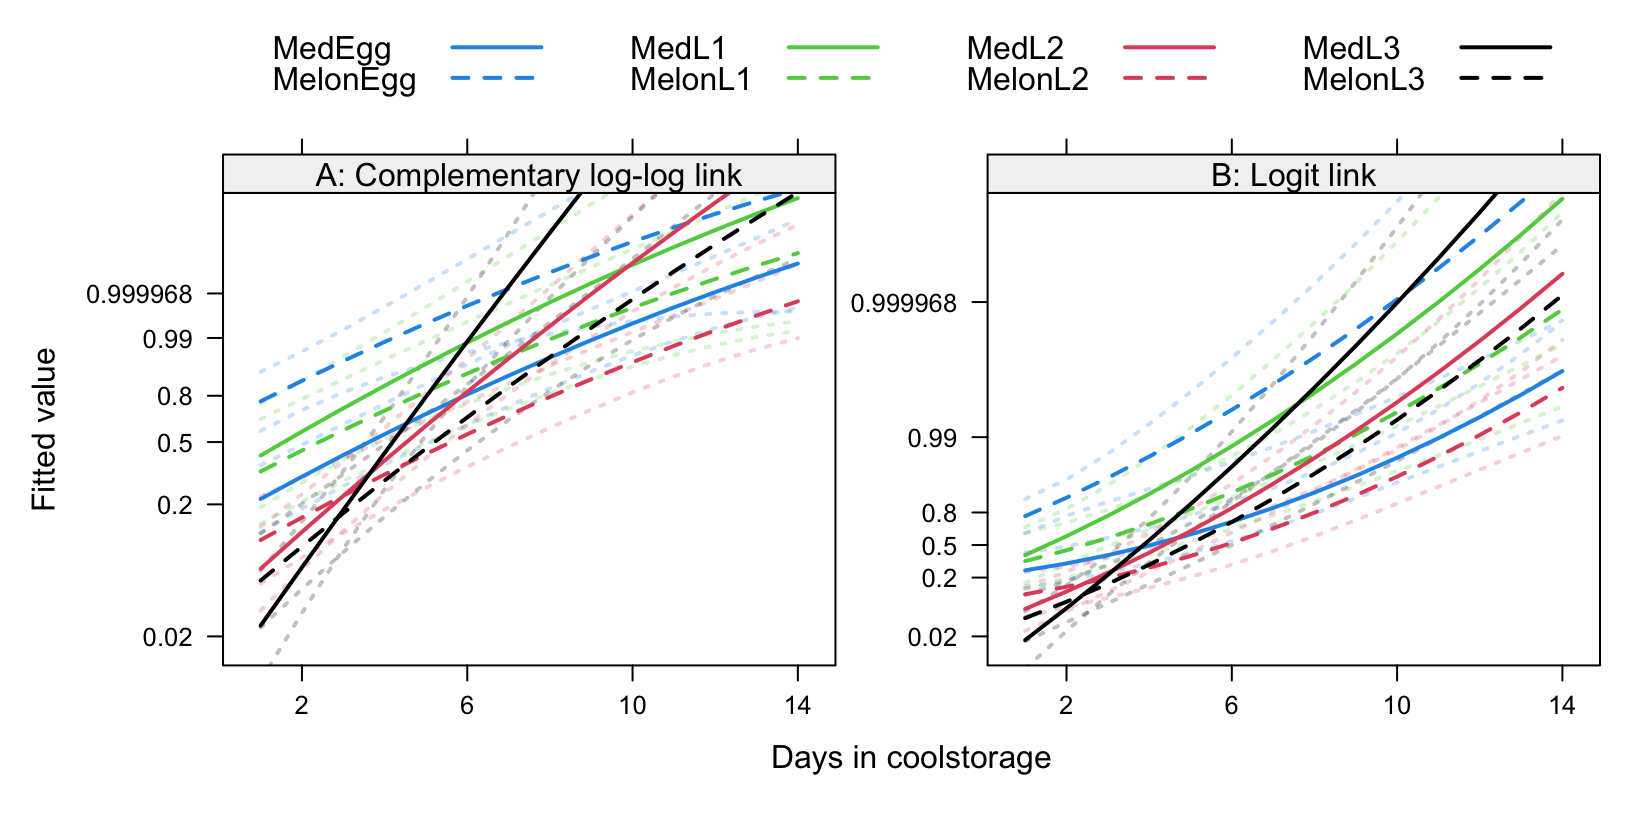
\includegraphics[width=1\textwidth,height=\textheight]{figs/g7_9-1.png}
\end{center}

\begin{Shaded}
\begin{Highlighting}[]
\NormalTok{dat }\OtherTok{\textless{}{-}} \FunctionTok{expand.grid}\NormalTok{(}\AttributeTok{trtGp=}\FunctionTok{factor}\NormalTok{(}\FunctionTok{levels}\NormalTok{(HawCon}\SpecialCharTok{$}\NormalTok{trtGp), }\AttributeTok{levels=}\FunctionTok{levels}\NormalTok{(HawCon}\SpecialCharTok{$}\NormalTok{trtGp)),}
\AttributeTok{TrtTime=}\FunctionTok{pretty}\NormalTok{(}\FunctionTok{range}\NormalTok{(HawCon}\SpecialCharTok{$}\NormalTok{TrtTime),}\DecValTok{15}\NormalTok{), }\AttributeTok{trtGpRep=}\ConstantTok{NA}\NormalTok{)}
\NormalTok{ab }\OtherTok{\textless{}{-}}\NormalTok{ qra}\SpecialCharTok{::}\FunctionTok{getScaleCoef}\NormalTok{(HawCon}\SpecialCharTok{$}\NormalTok{scTime)}
\NormalTok{dat}\SpecialCharTok{$}\NormalTok{scTime }\OtherTok{\textless{}{-}} \FunctionTok{with}\NormalTok{(dat,(TrtTime}\SpecialCharTok{{-}}\NormalTok{ab[}\DecValTok{1}\NormalTok{])}\SpecialCharTok{/}\NormalTok{ab[}\DecValTok{2}\NormalTok{])}
\NormalTok{hatClog }\OtherTok{\textless{}{-}} \FunctionTok{predict}\NormalTok{(HCbb2s.cll, }\AttributeTok{newdata=}\NormalTok{dat)}
\NormalTok{hatClog }\OtherTok{\textless{}{-}} \FunctionTok{predict}\NormalTok{(HCbb2s.cll, }\AttributeTok{se=}\NormalTok{T, }\AttributeTok{newdata=}\NormalTok{dat)}
\NormalTok{hatLgt }\OtherTok{\textless{}{-}} \FunctionTok{predict}\NormalTok{(HCbb2s.logit, }\AttributeTok{newdata=}\NormalTok{dat)}
\NormalTok{hatLgt }\OtherTok{\textless{}{-}} \FunctionTok{predict}\NormalTok{(HCbb2s.logit, }\AttributeTok{se=}\NormalTok{T, }\AttributeTok{newdata=}\NormalTok{dat)}
\NormalTok{dat2 }\OtherTok{\textless{}{-}} \FunctionTok{cbind}\NormalTok{(}\FunctionTok{rbind}\NormalTok{(dat,dat), }\AttributeTok{link=}\FunctionTok{rep}\NormalTok{(}\FunctionTok{c}\NormalTok{(}\StringTok{\textquotesingle{}clog\textquotesingle{}}\NormalTok{,}\StringTok{\textquotesingle{}logit\textquotesingle{}}\NormalTok{), }\FunctionTok{rep}\NormalTok{(}\FunctionTok{nrow}\NormalTok{(dat),}\DecValTok{2}\NormalTok{)))}
\NormalTok{dat2 }\OtherTok{\textless{}{-}} \FunctionTok{within}\NormalTok{(dat2, \{fit}\OtherTok{\textless{}{-}}\FunctionTok{c}\NormalTok{(hatClog}\SpecialCharTok{$}\NormalTok{fit,hatLgt}\SpecialCharTok{$}\NormalTok{fit);}
\NormalTok{se.fit}\OtherTok{\textless{}{-}}\FunctionTok{c}\NormalTok{(hatClog}\SpecialCharTok{$}\NormalTok{se.fit,hatLgt}\SpecialCharTok{$}\NormalTok{se.fit);}
\NormalTok{link}\OtherTok{=}\FunctionTok{rep}\NormalTok{(}\FunctionTok{c}\NormalTok{(}\StringTok{\textquotesingle{}clog\textquotesingle{}}\NormalTok{,}\StringTok{\textquotesingle{}logit\textquotesingle{}}\NormalTok{), }\FunctionTok{rep}\NormalTok{(}\FunctionTok{nrow}\NormalTok{(dat),}\DecValTok{2}\NormalTok{))\})}
\NormalTok{dat2 }\OtherTok{\textless{}{-}} \FunctionTok{within}\NormalTok{(dat2, \{lwr}\OtherTok{\textless{}{-}}\NormalTok{fit}\DecValTok{{-}2}\SpecialCharTok{*}\NormalTok{se.fit; upr}\OtherTok{\textless{}{-}}\NormalTok{fit}\SpecialCharTok{+}\DecValTok{2}\SpecialCharTok{*}\NormalTok{se.fit\})}
\FunctionTok{library}\NormalTok{(lattice)}
\NormalTok{my.panel.bands }\OtherTok{\textless{}{-}} \ControlFlowTok{function}\NormalTok{(x, y, upper, lower, fill, col,}
\NormalTok{subscripts, ..., font, fontface)}
\NormalTok{\{}
\NormalTok{upper }\OtherTok{\textless{}{-}}\NormalTok{ upper[subscripts]}
\NormalTok{lower }\OtherTok{\textless{}{-}}\NormalTok{ lower[subscripts]}
\FunctionTok{panel.lines}\NormalTok{(x,lower, ...)}
\FunctionTok{panel.lines}\NormalTok{(x,upper, ...)}
\NormalTok{\}}
\NormalTok{panel2 }\OtherTok{\textless{}{-}} \ControlFlowTok{function}\NormalTok{(x, y, ...)\{}
\FunctionTok{panel.superpose}\NormalTok{(x, y, }\AttributeTok{panel.groups =}\NormalTok{ my.panel.bands, }\AttributeTok{type=}\StringTok{\textquotesingle{}l\textquotesingle{}}\NormalTok{, }\AttributeTok{lty=}\DecValTok{3}\NormalTok{, }\AttributeTok{alpha=}\FloatTok{0.25}\NormalTok{,...)}
\FunctionTok{panel.xyplot}\NormalTok{(x, y, }\AttributeTok{type=}\StringTok{\textquotesingle{}l\textquotesingle{}}\NormalTok{, }\AttributeTok{lwd=}\DecValTok{2}\NormalTok{, }\AttributeTok{cex=}\FloatTok{0.6}\NormalTok{, ...)}
\NormalTok{\}}
\NormalTok{parset }\OtherTok{\textless{}{-}} \FunctionTok{simpleTheme}\NormalTok{(}\AttributeTok{col=}\FunctionTok{rep}\NormalTok{(}\DecValTok{4}\SpecialCharTok{:}\DecValTok{1}\NormalTok{,}\FunctionTok{rep}\NormalTok{(}\DecValTok{2}\NormalTok{,}\DecValTok{4}\NormalTok{)), }\AttributeTok{lty=}\FunctionTok{rep}\NormalTok{(}\DecValTok{1}\SpecialCharTok{:}\DecValTok{2}\NormalTok{, }\DecValTok{4}\NormalTok{), }\AttributeTok{lwd=}\DecValTok{2}\NormalTok{)}
\DocumentationTok{\#\# c(\textquotesingle{}solid\textquotesingle{},\textquotesingle{}1141\textquotesingle{})}
\NormalTok{p }\OtherTok{\textless{}{-}} \FunctionTok{c}\NormalTok{(.}\DecValTok{02}\NormalTok{,.}\DecValTok{2}\NormalTok{,.}\DecValTok{5}\NormalTok{,.}\DecValTok{8}\NormalTok{, .}\DecValTok{99}\NormalTok{, .}\DecValTok{999968}\NormalTok{)}
\NormalTok{cloglog }\OtherTok{\textless{}{-}} \FunctionTok{make.link}\NormalTok{(}\StringTok{\textquotesingle{}cloglog\textquotesingle{}}\NormalTok{)}\SpecialCharTok{$}\NormalTok{linkfun}
\NormalTok{logit }\OtherTok{\textless{}{-}} \FunctionTok{make.link}\NormalTok{(}\StringTok{\textquotesingle{}logit\textquotesingle{}}\NormalTok{)}\SpecialCharTok{$}\NormalTok{linkfun}
\NormalTok{fitpos }\OtherTok{\textless{}{-}} \FunctionTok{list}\NormalTok{(}\FunctionTok{cloglog}\NormalTok{(p), }\FunctionTok{logit}\NormalTok{(p))}
\NormalTok{lab }\OtherTok{\textless{}{-}} \FunctionTok{paste}\NormalTok{(p)}
\NormalTok{lim }\OtherTok{\textless{}{-}} \FunctionTok{list}\NormalTok{(}\FunctionTok{cloglog}\NormalTok{(}\FunctionTok{c}\NormalTok{(}\FloatTok{0.02}\NormalTok{, }\FloatTok{0.99998}\NormalTok{)), }\FunctionTok{logit}\NormalTok{(}\FunctionTok{c}\NormalTok{(}\FloatTok{0.02}\NormalTok{, }\FloatTok{0.99998}\NormalTok{)))}
\NormalTok{lim }\OtherTok{\textless{}{-}} \FunctionTok{lapply}\NormalTok{(lim, }\ControlFlowTok{function}\NormalTok{(x)}\FunctionTok{c}\NormalTok{(x[}\DecValTok{1}\NormalTok{],x[}\DecValTok{1}\NormalTok{]}\SpecialCharTok{+}\FunctionTok{diff}\NormalTok{(x)}\SpecialCharTok{*}\FloatTok{1.2}\NormalTok{))}

\NormalTok{gph }\OtherTok{\textless{}{-}} \FunctionTok{xyplot}\NormalTok{(fit}\SpecialCharTok{\textasciitilde{}}\NormalTok{TrtTime}\SpecialCharTok{|}\NormalTok{link, }\AttributeTok{outer=}\ConstantTok{TRUE}\NormalTok{, }\AttributeTok{data=}\NormalTok{dat2, }\AttributeTok{groups=}\NormalTok{trtGp,}
              \AttributeTok{upper =}\NormalTok{ dat2}\SpecialCharTok{$}\NormalTok{upr, }\AttributeTok{lower =}\NormalTok{ dat2}\SpecialCharTok{$}\NormalTok{lwr, }\AttributeTok{panel =}\NormalTok{ panel2,}
              \AttributeTok{xlab=}\StringTok{"Days in coolstorage"}\NormalTok{, }\AttributeTok{ylab=}\StringTok{"Fitted value"}\NormalTok{,}
              \AttributeTok{auto.key=}\FunctionTok{list}\NormalTok{(}\AttributeTok{text=}\FunctionTok{levels}\NormalTok{(HawCon}\SpecialCharTok{$}\NormalTok{trtGp), }\AttributeTok{columns=}\DecValTok{4}\NormalTok{,}
                            \AttributeTok{points=}\ConstantTok{FALSE}\NormalTok{, }\AttributeTok{lines=}\ConstantTok{TRUE}\NormalTok{),}
              \AttributeTok{par.settings=}\NormalTok{parset, }\AttributeTok{layout=}\FunctionTok{c}\NormalTok{(}\DecValTok{2}\NormalTok{,}\DecValTok{1}\NormalTok{),}
              \AttributeTok{scales=}\FunctionTok{list}\NormalTok{(}\AttributeTok{x=}\FunctionTok{list}\NormalTok{(}\AttributeTok{at=}\FunctionTok{c}\NormalTok{(}\DecValTok{2}\NormalTok{,}\DecValTok{6}\NormalTok{,}\DecValTok{10}\NormalTok{,}\DecValTok{14}\NormalTok{)),}
              \AttributeTok{y=}\FunctionTok{list}\NormalTok{(}\AttributeTok{relation=}\StringTok{\textquotesingle{}free\textquotesingle{}}\NormalTok{,}
              \AttributeTok{at=}\NormalTok{fitpos, }\AttributeTok{labels=}\NormalTok{lab, }\AttributeTok{limits=}\NormalTok{lim), }\AttributeTok{alternating=}\FunctionTok{c}\NormalTok{(}\DecValTok{1}\NormalTok{,}\DecValTok{1}\NormalTok{)))}
\FunctionTok{update}\NormalTok{(gph, }\AttributeTok{strip=}\FunctionTok{strip.custom}\NormalTok{(}\AttributeTok{factor.levels=}\FunctionTok{c}\NormalTok{(}\StringTok{"A: Complementary log{-}log link"}\NormalTok{,}
\StringTok{"B: Logit link"}\NormalTok{)))}
\end{Highlighting}
\end{Shaded}

\begin{center}
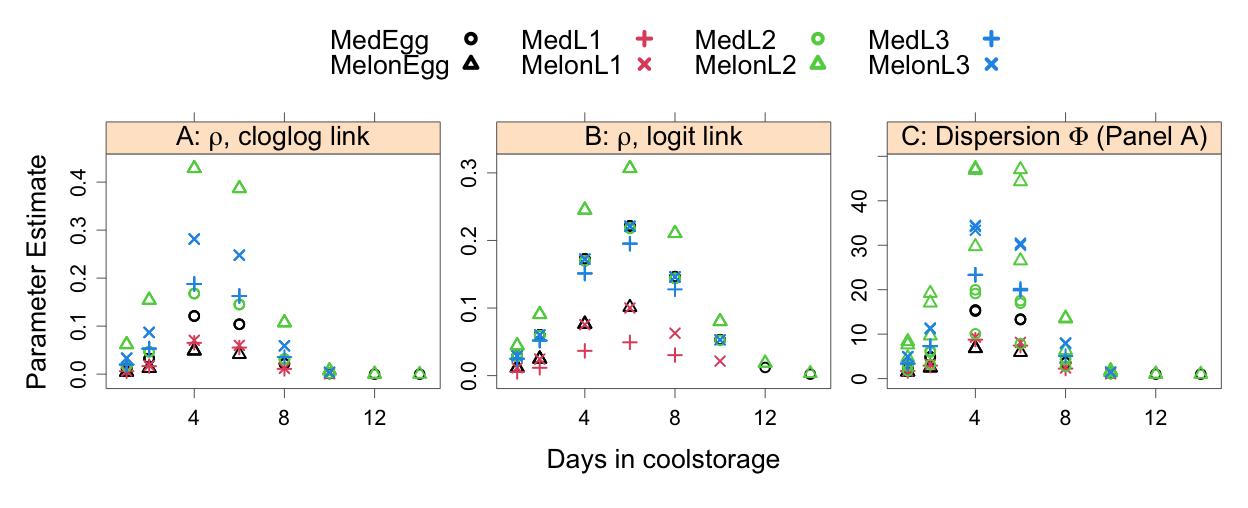
\includegraphics[width=1\textwidth,height=\textheight]{figs/g7_10-1.png}
\end{center}

\begin{Shaded}
\begin{Highlighting}[]
\NormalTok{parset }\OtherTok{\textless{}{-}}\NormalTok{ DAAG}\SpecialCharTok{::}\FunctionTok{DAAGtheme}\NormalTok{(}\AttributeTok{color=}\ConstantTok{TRUE}\NormalTok{, }\AttributeTok{col.points=}\FunctionTok{rep}\NormalTok{(}\DecValTok{1}\SpecialCharTok{:}\DecValTok{4}\NormalTok{,}\FunctionTok{rep}\NormalTok{(}\DecValTok{2}\NormalTok{,}\DecValTok{4}\NormalTok{)),}
                          \AttributeTok{pch=}\FunctionTok{rep}\NormalTok{(}\DecValTok{1}\SpecialCharTok{:}\DecValTok{4}\NormalTok{,}\DecValTok{2}\NormalTok{), }\AttributeTok{lwd=}\DecValTok{2}\NormalTok{)}
\NormalTok{HawCon}\SpecialCharTok{$}\NormalTok{rho2clog }\OtherTok{\textless{}{-}}\NormalTok{ qra}\SpecialCharTok{::}\FunctionTok{getRho}\NormalTok{(HCbb.cll)}
\NormalTok{HawCon}\SpecialCharTok{$}\NormalTok{dispClog }\OtherTok{\textless{}{-}} \FunctionTok{with}\NormalTok{(HawCon, }\DecValTok{1}\SpecialCharTok{+}\NormalTok{(Total}\DecValTok{{-}1}\NormalTok{)}\SpecialCharTok{*}\NormalTok{rho2clog)}
\FunctionTok{par}\NormalTok{(}\AttributeTok{oma=}\FunctionTok{c}\NormalTok{(}\DecValTok{0}\NormalTok{,}\DecValTok{0}\NormalTok{,}\DecValTok{2}\NormalTok{,}\DecValTok{0}\NormalTok{))}
\NormalTok{titles}\OtherTok{=}\FunctionTok{c}\NormalTok{(}\FunctionTok{expression}\NormalTok{(}\StringTok{"A: "}\SpecialCharTok{*}\NormalTok{rho}\SpecialCharTok{*}\StringTok{", cloglog link"}\NormalTok{),}\FunctionTok{expression}\NormalTok{(}\StringTok{"B: "}\SpecialCharTok{*}\NormalTok{rho}\SpecialCharTok{*}\StringTok{", logit link"}\NormalTok{),}
\FunctionTok{expression}\NormalTok{(}\StringTok{"C: Dispersion "}\SpecialCharTok{*}\NormalTok{Phi}\SpecialCharTok{*}\StringTok{" (Panel A)"}\NormalTok{))}
\FunctionTok{library}\NormalTok{(lattice)}
\NormalTok{HawCon}\SpecialCharTok{$}\NormalTok{rho2logit }\OtherTok{\textless{}{-}}\NormalTok{ qra}\SpecialCharTok{::}\FunctionTok{getRho}\NormalTok{(HCbb.logit)}
\FunctionTok{xyplot}\NormalTok{(rho2clog}\SpecialCharTok{+}\NormalTok{rho2logit}\SpecialCharTok{+}\NormalTok{dispClog }\SpecialCharTok{\textasciitilde{}}\NormalTok{ TrtTime, }\AttributeTok{groups=}\NormalTok{trtGp, }\AttributeTok{data=}\NormalTok{HawCon,}
       \AttributeTok{outer=}\ConstantTok{TRUE}\NormalTok{, }\AttributeTok{between=}\FunctionTok{list}\NormalTok{(}\AttributeTok{x=}\FloatTok{0.25}\NormalTok{), }\AttributeTok{par.settings=}\NormalTok{parset,}
   \AttributeTok{scales=}\FunctionTok{list}\NormalTok{(}\AttributeTok{x=}\FunctionTok{list}\NormalTok{(}\AttributeTok{alternating=}\ConstantTok{FALSE}\NormalTok{,}\AttributeTok{at=}\FunctionTok{c}\NormalTok{(}\DecValTok{4}\NormalTok{,}\DecValTok{8}\NormalTok{,}\DecValTok{12}\NormalTok{), }\AttributeTok{labels=}\FunctionTok{paste}\NormalTok{(}\FunctionTok{c}\NormalTok{(}\DecValTok{4}\NormalTok{,}\DecValTok{8}\NormalTok{,}\DecValTok{12}\NormalTok{))),}
               \AttributeTok{y=}\FunctionTok{list}\NormalTok{(}\AttributeTok{relation=}\StringTok{\textquotesingle{}free\textquotesingle{}}\NormalTok{,}\AttributeTok{tick.number=}\DecValTok{4}\NormalTok{)),}
   \AttributeTok{auto.key=}\FunctionTok{list}\NormalTok{(}\AttributeTok{columns=}\DecValTok{4}\NormalTok{, }\AttributeTok{between.columns=}\DecValTok{2}\NormalTok{, }\AttributeTok{between=}\DecValTok{1}\NormalTok{),}
   \AttributeTok{xlab=}\StringTok{"Days in coolstorage"}\NormalTok{, }\AttributeTok{ylab=}\StringTok{"Parameter Estimate"}\NormalTok{,}
   \AttributeTok{strip=}\FunctionTok{strip.custom}\NormalTok{(}\AttributeTok{factor.levels=}\NormalTok{titles))}
\end{Highlighting}
\end{Shaded}

\subsubsection{Subsection 7.6.2: Diagnostic
checks}\label{subsection-7.6.2-diagnostic-checks}

\begin{center}
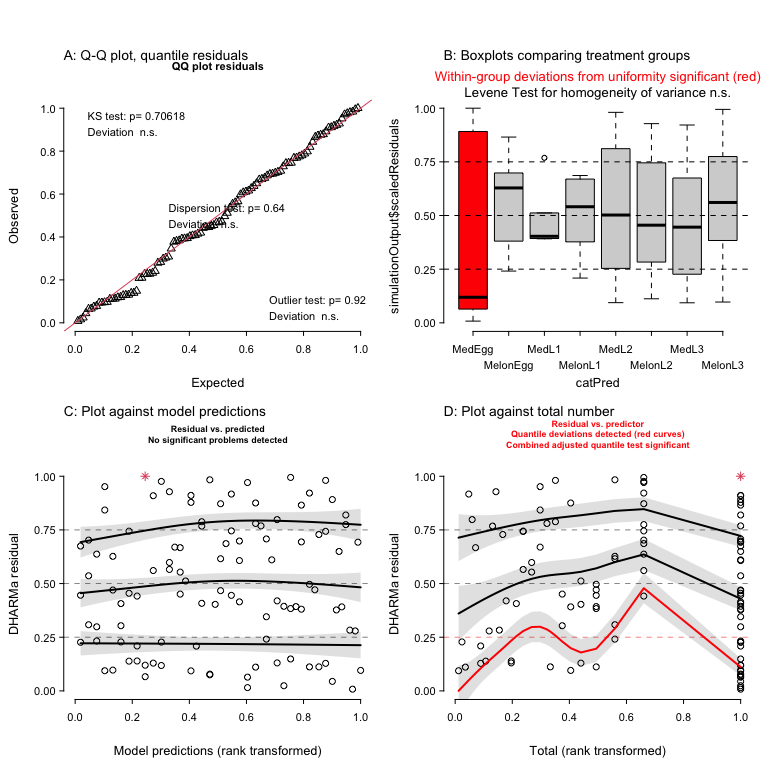
\includegraphics[width=1\textwidth,height=\textheight]{figs/g7_11-1.png}
\end{center}

\begin{Shaded}
\begin{Highlighting}[]
\FunctionTok{par}\NormalTok{(}\AttributeTok{oma=}\FunctionTok{c}\NormalTok{(}\DecValTok{0}\NormalTok{,}\DecValTok{0}\NormalTok{,}\DecValTok{2}\NormalTok{,}\FloatTok{0.5}\NormalTok{))}
\DocumentationTok{\#\# Code for plots, excluding main titles}
\FunctionTok{set.seed}\NormalTok{(}\DecValTok{29}\NormalTok{)}
\NormalTok{simRef }\OtherTok{\textless{}{-}}\NormalTok{ DHARMa}\SpecialCharTok{::}\FunctionTok{simulateResiduals}\NormalTok{(HCbb.cll, }\AttributeTok{n=}\DecValTok{250}\NormalTok{, }\AttributeTok{seed=}\ConstantTok{FALSE}\NormalTok{)}
\NormalTok{DHARMa}\SpecialCharTok{::}\FunctionTok{plotQQunif}\NormalTok{(simRef)}
\FunctionTok{title}\NormalTok{(}\AttributeTok{main=}\StringTok{"A: Q{-}Q plot, quantile residuals"}\NormalTok{, }\AttributeTok{adj=}\DecValTok{0}\NormalTok{, }\AttributeTok{line=}\FloatTok{2.5}\NormalTok{, }
      \AttributeTok{font.main=}\DecValTok{1}\NormalTok{, }\AttributeTok{cex.main=}\FloatTok{1.25}\NormalTok{)}
\NormalTok{DHARMa}\SpecialCharTok{::}\FunctionTok{plotResiduals}\NormalTok{(simRef, }\AttributeTok{form=}\NormalTok{HawCon}\SpecialCharTok{$}\NormalTok{trtGp)}
\FunctionTok{axis}\NormalTok{(}\DecValTok{1}\NormalTok{, }\AttributeTok{at=}\FunctionTok{c}\NormalTok{(}\DecValTok{2}\NormalTok{,}\DecValTok{4}\NormalTok{,}\DecValTok{6}\NormalTok{,}\DecValTok{8}\NormalTok{), }\AttributeTok{labels=}\FunctionTok{levels}\NormalTok{(HawCon}\SpecialCharTok{$}\NormalTok{trtGp)[}\FunctionTok{c}\NormalTok{(}\DecValTok{2}\NormalTok{,}\DecValTok{4}\NormalTok{,}\DecValTok{6}\NormalTok{,}\DecValTok{8}\NormalTok{)],}
     \AttributeTok{gap.axis=}\DecValTok{0}\NormalTok{, }\AttributeTok{line=}\DecValTok{1}\NormalTok{, }\AttributeTok{lwd=}\DecValTok{0}\NormalTok{)}
\FunctionTok{title}\NormalTok{(}\AttributeTok{main=}\StringTok{"B: Boxplots comparing treatment groups"}\NormalTok{, }\AttributeTok{adj=}\DecValTok{0}\NormalTok{, }\AttributeTok{line=}\FloatTok{2.5}\NormalTok{,}
      \AttributeTok{font.main=}\DecValTok{1}\NormalTok{, }\AttributeTok{cex.main=}\FloatTok{1.25}\NormalTok{)}
\NormalTok{DHARMa}\SpecialCharTok{::}\FunctionTok{plotResiduals}\NormalTok{(simRef)}
\FunctionTok{title}\NormalTok{(}\AttributeTok{main=}\StringTok{"C: Plot against model predictions"}\NormalTok{, }\AttributeTok{adj=}\DecValTok{0}\NormalTok{, }\AttributeTok{font.main=}\DecValTok{1}\NormalTok{, }\AttributeTok{line=}\FloatTok{3.25}\NormalTok{,}
       \AttributeTok{cex.main=}\FloatTok{1.25}\NormalTok{)}
\NormalTok{DHARMa}\SpecialCharTok{::}\FunctionTok{plotResiduals}\NormalTok{(simRef, }\AttributeTok{form=}\NormalTok{HawCon}\SpecialCharTok{$}\NormalTok{Total)}
\FunctionTok{title}\NormalTok{(}\AttributeTok{main=}\StringTok{"D: Plot against total number"}\NormalTok{, }\AttributeTok{adj=}\DecValTok{0}\NormalTok{, }\AttributeTok{font.main=}\DecValTok{1}\NormalTok{, }\AttributeTok{line=}\FloatTok{3.25}\NormalTok{,}
       \AttributeTok{cex.main=}\FloatTok{1.25}\NormalTok{)}
\end{Highlighting}
\end{Shaded}

\subsubsection{Subsection 7.6.3: Lethal time estimates and confidence
intervals}\label{subsection-7.6.3-lethal-time-estimates-and-confidence-intervals}

\begin{Shaded}
\begin{Highlighting}[]
\NormalTok{shorten }\OtherTok{\textless{}{-}} \ControlFlowTok{function}\NormalTok{(nam, }\AttributeTok{leaveout=}\FunctionTok{c}\NormalTok{(}\StringTok{\textquotesingle{}trtGp\textquotesingle{}}\NormalTok{,}\StringTok{\textquotesingle{}Fly\textquotesingle{}}\NormalTok{,}\StringTok{\textquotesingle{}:\textquotesingle{}}\NormalTok{))\{}
\ControlFlowTok{for}\NormalTok{(txt }\ControlFlowTok{in}\NormalTok{ leaveout)\{}
\NormalTok{nam }\OtherTok{\textless{}{-}} \FunctionTok{gsub}\NormalTok{(txt,}\StringTok{\textquotesingle{}\textquotesingle{}}\NormalTok{, nam, }\AttributeTok{fixed=}\ConstantTok{TRUE}\NormalTok{)}
\NormalTok{\}}
\NormalTok{nam}
\NormalTok{\}}
\end{Highlighting}
\end{Shaded}

\begin{Shaded}
\begin{Highlighting}[]
\NormalTok{LTbb.cll }\OtherTok{\textless{}{-}}\NormalTok{ qra}\SpecialCharTok{::}\FunctionTok{extractLT}\NormalTok{(}\AttributeTok{p=}\FloatTok{0.99}\NormalTok{, }\AttributeTok{obj=}\NormalTok{HCbb.cll, }\AttributeTok{link=}\StringTok{"cloglog"}\NormalTok{,}
                        \AttributeTok{a=}\DecValTok{1}\SpecialCharTok{:}\DecValTok{8}\NormalTok{, }\AttributeTok{b=}\DecValTok{9}\SpecialCharTok{:}\DecValTok{16}\NormalTok{, }\AttributeTok{eps=}\DecValTok{0}\NormalTok{, }\AttributeTok{df.t=}\ConstantTok{NULL}\NormalTok{)[,}\SpecialCharTok{{-}}\DecValTok{2}\NormalTok{]}
\FunctionTok{rownames}\NormalTok{(LTbb.cll) }\OtherTok{\textless{}{-}} \FunctionTok{gsub}\NormalTok{(}\StringTok{"trtGp|Fly|:"}\NormalTok{, }\StringTok{\textquotesingle{}\textquotesingle{}}\NormalTok{, }\FunctionTok{rownames}\NormalTok{(LTbb.cll), }\AttributeTok{perl=}\NormalTok{T)}
\end{Highlighting}
\end{Shaded}

\begin{Shaded}
\begin{Highlighting}[]
\NormalTok{LTbb.logit }\OtherTok{\textless{}{-}}\NormalTok{ qra}\SpecialCharTok{::}\FunctionTok{extractLT}\NormalTok{(}\AttributeTok{p=}\FloatTok{0.99}\NormalTok{, }\AttributeTok{obj=}\NormalTok{HCbb.logit, }\AttributeTok{link=}\StringTok{"logit"}\NormalTok{,}
                             \AttributeTok{a=}\DecValTok{1}\SpecialCharTok{:}\DecValTok{8}\NormalTok{, }\AttributeTok{b=}\DecValTok{9}\SpecialCharTok{:}\DecValTok{16}\NormalTok{, }\AttributeTok{eps=}\DecValTok{0}\NormalTok{, }\AttributeTok{offset=}\DecValTok{0}\NormalTok{,}
\AttributeTok{df.t=}\ConstantTok{NULL}\NormalTok{)[,}\SpecialCharTok{{-}}\DecValTok{2}\NormalTok{]}
\FunctionTok{rownames}\NormalTok{(LTbb.logit) }\OtherTok{\textless{}{-}} \FunctionTok{shorten}\NormalTok{(}\FunctionTok{rownames}\NormalTok{(LTbb.logit))}
\end{Highlighting}
\end{Shaded}

\begin{center}
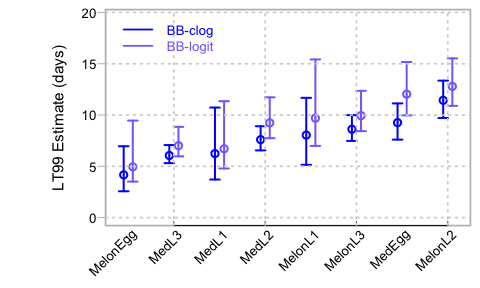
\includegraphics[width=0.65\textwidth,height=\textheight]{figs/g7_12-1.png}
\end{center}

\begin{Shaded}
\begin{Highlighting}[]
\FunctionTok{library}\NormalTok{(plotrix)}
\NormalTok{gpNam }\OtherTok{\textless{}{-}} \FunctionTok{rownames}\NormalTok{(LTbb.cll)}
\NormalTok{ordEst }\OtherTok{\textless{}{-}} \FunctionTok{order}\NormalTok{(LTbb.cll[,}\DecValTok{1}\NormalTok{])}
\NormalTok{col5 }\OtherTok{\textless{}{-}} \FunctionTok{c}\NormalTok{(}\StringTok{"blue"}\NormalTok{,}\StringTok{"lightslateblue"}\NormalTok{,}\StringTok{"blueviolet"}\NormalTok{,}\StringTok{\textquotesingle{}gray50\textquotesingle{}}\NormalTok{,}\StringTok{\textquotesingle{}gray80\textquotesingle{}}\NormalTok{)}
\FunctionTok{plotCI}\NormalTok{(}\DecValTok{1}\SpecialCharTok{:}\DecValTok{8}\FloatTok{{-}0.1}\NormalTok{, }\AttributeTok{y=}\NormalTok{LTbb.cll[ordEst,}\DecValTok{1}\NormalTok{], }\AttributeTok{ui=}\NormalTok{LTbb.cll[ordEst,}\DecValTok{3}\NormalTok{],}
  \AttributeTok{li=}\NormalTok{LTbb.cll[ordEst,}\DecValTok{2}\NormalTok{], }\AttributeTok{lwd=}\DecValTok{2}\NormalTok{, }\AttributeTok{col=}\NormalTok{col5[}\DecValTok{1}\NormalTok{], }\AttributeTok{xaxt=}\StringTok{"n"}\NormalTok{,}
  \AttributeTok{fg=}\StringTok{"gray"}\NormalTok{, }\AttributeTok{xlab=}\StringTok{""}\NormalTok{, }\AttributeTok{ylab=}\StringTok{"LT99 Estimate (days)"}\NormalTok{,}
  \AttributeTok{xlim=}\FunctionTok{c}\NormalTok{(}\FloatTok{0.8}\NormalTok{,}\FloatTok{8.2}\NormalTok{), }\AttributeTok{ylim=}\FunctionTok{c}\NormalTok{(}\DecValTok{0}\NormalTok{,}\FloatTok{19.5}\NormalTok{))}
\FunctionTok{plotCI}\NormalTok{(}\DecValTok{1}\SpecialCharTok{:}\DecValTok{8}\FloatTok{+0.1}\NormalTok{, }\AttributeTok{y=}\NormalTok{LTbb.logit[ordEst,}\DecValTok{1}\NormalTok{], }\AttributeTok{ui=}\NormalTok{LTbb.logit[ordEst,}\DecValTok{3}\NormalTok{],}
  \AttributeTok{li=}\NormalTok{LTbb.logit[ordEst,}\DecValTok{2}\NormalTok{], }\AttributeTok{lwd=}\DecValTok{2}\NormalTok{, }\AttributeTok{col=}\NormalTok{col5[}\DecValTok{2}\NormalTok{], }\AttributeTok{xaxt=}\StringTok{"n"}\NormalTok{, }\AttributeTok{add=}\ConstantTok{TRUE}\NormalTok{)}
\FunctionTok{axis}\NormalTok{(}\DecValTok{1}\NormalTok{, }\AttributeTok{labels=}\ConstantTok{FALSE}\NormalTok{, }\AttributeTok{tck=}\FloatTok{0.02}\NormalTok{, }\AttributeTok{col.ticks=}\StringTok{"gray40"}\NormalTok{)}
\FunctionTok{text}\NormalTok{(}\AttributeTok{x =} \DecValTok{1}\SpecialCharTok{:}\FunctionTok{length}\NormalTok{(gpNam)}\SpecialCharTok{+}\FloatTok{0.1}\NormalTok{,}
  \DocumentationTok{\#\# Move labels to just below bottom of chart.}
  \AttributeTok{y =} \FunctionTok{par}\NormalTok{(}\StringTok{"usr"}\NormalTok{)[}\DecValTok{3}\NormalTok{] }\SpecialCharTok{{-}} \FloatTok{0.8}\NormalTok{,}
  \AttributeTok{labels =}\NormalTok{ gpNam[ordEst], }\DocumentationTok{\#\# Use names from the data list.}
    \AttributeTok{xpd =} \ConstantTok{NA}\NormalTok{,        }\DocumentationTok{\#\# Change the clipping region}
  \AttributeTok{srt =} \DecValTok{45}\NormalTok{,          }\DocumentationTok{\#\# Rotate the labels by 45 degrees.}
  \AttributeTok{adj =} \FloatTok{0.95}\NormalTok{)        }\DocumentationTok{\#\# Adjust the labels to almost 100\% right{-}justified}
\FunctionTok{grid}\NormalTok{()}
\FunctionTok{legend}\NormalTok{(}\StringTok{"topleft"}\NormalTok{, }\AttributeTok{legend=}\FunctionTok{c}\NormalTok{(}\StringTok{"BB{-}clog"}\NormalTok{, }\StringTok{"BB{-}logit"}\NormalTok{),}
       \AttributeTok{inset=}\FunctionTok{c}\NormalTok{(}\FloatTok{0.01}\NormalTok{,}\FloatTok{0.01}\NormalTok{), }\AttributeTok{lty=}\FunctionTok{c}\NormalTok{(}\DecValTok{1}\NormalTok{,}\DecValTok{1}\NormalTok{), }\AttributeTok{col=}\NormalTok{col5[}\DecValTok{1}\SpecialCharTok{:}\DecValTok{2}\NormalTok{],}
\AttributeTok{text.col=}\NormalTok{col5[}\DecValTok{1}\SpecialCharTok{:}\DecValTok{2}\NormalTok{], }\AttributeTok{bty=}\StringTok{"n"}\NormalTok{,}\AttributeTok{y.intersp=}\FloatTok{0.85}\NormalTok{)}
\end{Highlighting}
\end{Shaded}

\begin{Shaded}
\begin{Highlighting}[]
\NormalTok{HCbin.cll }\OtherTok{\textless{}{-}} \FunctionTok{glmmTMB}\NormalTok{(}\FunctionTok{cbind}\NormalTok{(Dead,Live)}\SpecialCharTok{\textasciitilde{}}\DecValTok{0}\SpecialCharTok{+}\NormalTok{trtGp}\SpecialCharTok{/}\NormalTok{TrtTime}\SpecialCharTok{+}\NormalTok{(scTime}\SpecialCharTok{|}\NormalTok{trtGp),}
                     \AttributeTok{family=}\FunctionTok{binomial}\NormalTok{(}\AttributeTok{link=}\StringTok{"cloglog"}\NormalTok{), }\AttributeTok{data=}\NormalTok{HawCon)}
\end{Highlighting}
\end{Shaded}

\begin{Shaded}
\begin{Highlighting}[]
\NormalTok{LTbin.cll }\OtherTok{\textless{}{-}}\NormalTok{ qra}\SpecialCharTok{::}\FunctionTok{extractLT}\NormalTok{(}\AttributeTok{p=}\FloatTok{0.99}\NormalTok{, }\AttributeTok{obj=}\NormalTok{HCbin.cll,}
                            \AttributeTok{a=}\DecValTok{1}\SpecialCharTok{:}\DecValTok{8}\NormalTok{, }\AttributeTok{b=}\DecValTok{9}\SpecialCharTok{:}\DecValTok{16}\NormalTok{, }\AttributeTok{eps=}\DecValTok{0}\NormalTok{, }\AttributeTok{df.t=}\ConstantTok{NULL}\NormalTok{)[,}\SpecialCharTok{{-}}\DecValTok{2}\NormalTok{]}
\FunctionTok{rownames}\NormalTok{(LTbin.cll) }\OtherTok{\textless{}{-}} \FunctionTok{shorten}\NormalTok{(}\FunctionTok{rownames}\NormalTok{(LTbin.cll))}
\end{Highlighting}
\end{Shaded}

\paragraph{A warning against
over-interpretation}\label{a-warning-against-over-interpretation}

\subsection{\texorpdfstring{Section 7.7 Observation level random effects
--- the \texttt{moths}
dataset}{Section 7.7 Observation level random effects --- the moths dataset}}\label{section-7.7-observation-level-random-effects-the-moths-dataset}

\begin{Shaded}
\begin{Highlighting}[]
\NormalTok{moths }\OtherTok{\textless{}{-}}\NormalTok{ DAAG}\SpecialCharTok{::}\NormalTok{moths}
\NormalTok{moths}\SpecialCharTok{$}\NormalTok{transect }\OtherTok{\textless{}{-}} \DecValTok{1}\SpecialCharTok{:}\DecValTok{41}  \CommentTok{\# Each row is from a different transect}
\NormalTok{moths}\SpecialCharTok{$}\NormalTok{habitat }\OtherTok{\textless{}{-}} \FunctionTok{relevel}\NormalTok{(moths}\SpecialCharTok{$}\NormalTok{habitat, }\AttributeTok{ref=}\StringTok{"Lowerside"}\NormalTok{)}
\NormalTok{A.glmer }\OtherTok{\textless{}{-}}  \FunctionTok{glmer}\NormalTok{(A}\SpecialCharTok{\textasciitilde{}}\NormalTok{habitat}\SpecialCharTok{+}\FunctionTok{sqrt}\NormalTok{(meters)}\SpecialCharTok{+}\NormalTok{(}\DecValTok{1}\SpecialCharTok{|}\NormalTok{transect),}
\AttributeTok{family=}\FunctionTok{poisson}\NormalTok{(}\AttributeTok{link=}\NormalTok{sqrt), }\AttributeTok{data=}\NormalTok{moths)}
\FunctionTok{print}\NormalTok{(}\FunctionTok{summary}\NormalTok{(A.glmer), }\AttributeTok{show.resid=}\ConstantTok{FALSE}\NormalTok{, }\AttributeTok{correlation=}\ConstantTok{FALSE}\NormalTok{, }\AttributeTok{digits=}\DecValTok{3}\NormalTok{)}
\end{Highlighting}
\end{Shaded}

\begin{verbatim}
Generalized linear mixed model fit by maximum likelihood (Laplace
  Approximation) [glmerMod]
 Family: poisson  ( sqrt )
Formula: A ~ habitat + sqrt(meters) + (1 | transect)
   Data: moths

     AIC      BIC   logLik deviance df.resid 
   212.6    229.7    -96.3    192.6       31 

Random effects:
 Groups   Name        Variance Std.Dev.
 transect (Intercept) 0.319    0.564   
Number of obs: 41, groups:  transect, 41

Fixed effects:
                 Estimate Std. Error z value   Pr(>|z|)
(Intercept)        1.7322     0.3513    4.93 0.00000082
habitatBank       -2.0415     0.9377   -2.18      0.029
habitatDisturbed  -1.0359     0.4071   -2.54      0.011
habitatNEsoak     -0.7319     0.4323   -1.69      0.090
habitatNWsoak      2.6787     0.5101    5.25 0.00000015
habitatSEsoak      0.1178     0.3923    0.30      0.764
habitatSWsoak      0.3900     0.5260    0.74      0.458
habitatUpperside  -0.3135     0.7549   -0.42      0.678
sqrt(meters)       0.0675     0.0631    1.07      0.285
\end{verbatim}

\begin{Shaded}
\begin{Highlighting}[]
\FunctionTok{suppressPackageStartupMessages}\NormalTok{(}\FunctionTok{library}\NormalTok{(gamlss))}
\NormalTok{A1quasi.glm }\OtherTok{\textless{}{-}} \FunctionTok{glm}\NormalTok{(A}\SpecialCharTok{\textasciitilde{}}\NormalTok{habitat, }\AttributeTok{data=}\NormalTok{moths, }\AttributeTok{family=}\FunctionTok{quasipoisson}\NormalTok{(}\AttributeTok{link=}\NormalTok{sqrt))}
\NormalTok{Asqrt.lss }\OtherTok{\textless{}{-}} \FunctionTok{gamlss}\NormalTok{(A }\SpecialCharTok{\textasciitilde{}}\NormalTok{ habitat }\SpecialCharTok{+} \FunctionTok{sqrt}\NormalTok{(meters), }\AttributeTok{trace=}\ConstantTok{FALSE}\NormalTok{,}
                    \AttributeTok{family =} \FunctionTok{NBI}\NormalTok{(}\AttributeTok{mu.link=}\StringTok{\textquotesingle{}sqrt\textquotesingle{}}\NormalTok{), }\AttributeTok{data =}\NormalTok{ moths)}
\NormalTok{A1.glmer }\OtherTok{\textless{}{-}} \FunctionTok{glmer}\NormalTok{(A}\SpecialCharTok{\textasciitilde{}}\NormalTok{habitat}\SpecialCharTok{+}\NormalTok{(}\DecValTok{1}\SpecialCharTok{|}\NormalTok{transect), }\AttributeTok{data=}\NormalTok{moths, }\AttributeTok{family=}\FunctionTok{poisson}\NormalTok{(}\AttributeTok{link=}\NormalTok{sqrt))}
\end{Highlighting}
\end{Shaded}

\begin{Shaded}
\begin{Highlighting}[]
\NormalTok{Cglm }\OtherTok{\textless{}{-}} \FunctionTok{coef}\NormalTok{(}\FunctionTok{summary}\NormalTok{(A1quasi.glm))}
\NormalTok{Cglmer }\OtherTok{\textless{}{-}} \FunctionTok{coef}\NormalTok{(}\FunctionTok{summary}\NormalTok{(A1.glmer))}
\NormalTok{fitAll }\OtherTok{\textless{}{-}} \FunctionTok{cbind}\NormalTok{(}\StringTok{"quasi{-}Coef"}\OtherTok{=}\NormalTok{Cglm[}\SpecialCharTok{{-}}\DecValTok{1}\NormalTok{,}\DecValTok{1}\NormalTok{], }\StringTok{"quasi{-}SE"}\OtherTok{=}\NormalTok{Cglm[}\SpecialCharTok{{-}}\DecValTok{1}\NormalTok{,}\DecValTok{2}\NormalTok{],}
  \StringTok{"NBI{-}Coef"}\OtherTok{=}\FunctionTok{coef}\NormalTok{(Asqrt.lss)[}\DecValTok{2}\SpecialCharTok{:}\DecValTok{8}\NormalTok{], }\StringTok{"NBI{-}SE"}\OtherTok{=}\FunctionTok{c}\NormalTok{(}\FloatTok{0.94}\NormalTok{,.}\DecValTok{41}\NormalTok{,.}\DecValTok{43}\NormalTok{,.}\DecValTok{51}\NormalTok{,.}\DecValTok{39}\NormalTok{,.}\DecValTok{53}\NormalTok{,.}\DecValTok{75}\NormalTok{),}
  \StringTok{"glmer{-}Coef"}\OtherTok{=}\NormalTok{Cglmer[}\SpecialCharTok{{-}}\DecValTok{1}\NormalTok{,}\DecValTok{1}\NormalTok{], }\StringTok{"glmer{-}SE"}\OtherTok{=}\NormalTok{Cglmer[}\SpecialCharTok{{-}}\DecValTok{1}\NormalTok{,}\DecValTok{2}\NormalTok{])}
\FunctionTok{rownames}\NormalTok{(fitAll) }\OtherTok{\textless{}{-}} \FunctionTok{substring}\NormalTok{(}\FunctionTok{rownames}\NormalTok{(fitAll),}\DecValTok{8}\NormalTok{)}
\FunctionTok{round}\NormalTok{(fitAll, }\DecValTok{2}\NormalTok{)  }\CommentTok{\# NB, all SEs are for the difference from \textquotesingle{}Lowerside\textquotesingle{}}
\end{Highlighting}
\end{Shaded}

\begin{verbatim}
          quasi-Coef quasi-SE NBI-Coef NBI-SE glmer-Coef glmer-SE
Bank           -2.13     0.86    -2.19   0.94      -1.99     0.95
Disturbed      -1.07     0.41    -1.00   0.41      -1.13     0.40
NEsoak         -0.61     0.43    -0.80   0.43      -0.57     0.41
NWsoak          2.73     0.54     2.67   0.51       2.73     0.51
SEsoak          0.16     0.41     0.09   0.39       0.19     0.39
SWsoak          0.45     0.54     0.28   0.53       0.54     0.51
Upperside       0.23     0.45    -0.41   0.75       0.36     0.43
\end{verbatim}

\begin{Shaded}
\begin{Highlighting}[]
\FunctionTok{detach}\NormalTok{(}\StringTok{"package:glmmTMB"}\NormalTok{, }\AttributeTok{character.only=}\ConstantTok{TRUE}\NormalTok{)}
\end{Highlighting}
\end{Shaded}

\subsection{Section 7.8 Repeated measures in
time}\label{section-7.8-repeated-measures-in-time}

\paragraph{The theory of repeated measures
modeling}\label{the-theory-of-repeated-measures-modeling}

\paragraph{*Correlation structure}\label{correlation-structure}

\paragraph{Different approaches to repeated measures
analysis}\label{different-approaches-to-repeated-measures-analysis}

\subsubsection{Subsection 7.8.1: Example -- random variation between
profiles}\label{subsection-7.8.1-example-random-variation-between-profiles}

\begin{Shaded}
\begin{Highlighting}[]
\NormalTok{humanpower1 }\OtherTok{\textless{}{-}}\NormalTok{ DAAG}\SpecialCharTok{::}\NormalTok{humanpower1}
\end{Highlighting}
\end{Shaded}

\begin{center}
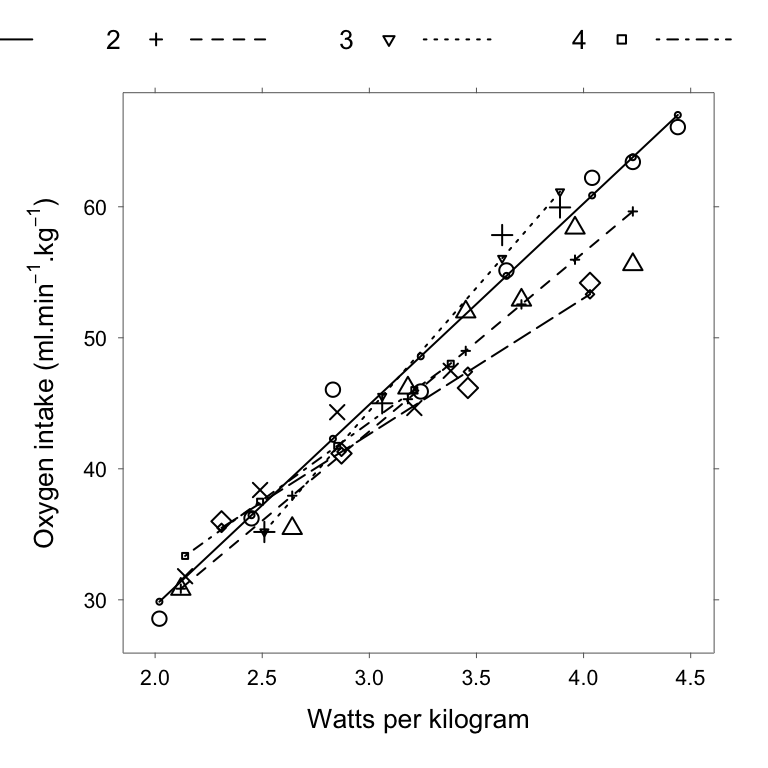
\includegraphics[width=0.5\textwidth,height=\textheight]{figs/g7_13-1.png}
\end{center}

\begin{Shaded}
\begin{Highlighting}[]
\DocumentationTok{\#\# Plot points and fitted lines}
\FunctionTok{xyplot}\NormalTok{(o2 }\SpecialCharTok{\textasciitilde{}}\NormalTok{ wattsPerKg, }\AttributeTok{groups=}\NormalTok{id, }\AttributeTok{data=}\NormalTok{humanpower1,}
       \AttributeTok{par.settings=}\NormalTok{DAAG}\SpecialCharTok{::}\FunctionTok{DAAGtheme}\NormalTok{(}\AttributeTok{color=}\NormalTok{F), }\AttributeTok{scales=}\FunctionTok{list}\NormalTok{(}\AttributeTok{tck=}\FloatTok{0.5}\NormalTok{),}
       \AttributeTok{panel=}\ControlFlowTok{function}\NormalTok{(x,y,subscripts,groups,...)\{}
\NormalTok{                yhat }\OtherTok{\textless{}{-}} \FunctionTok{fitted}\NormalTok{(}\FunctionTok{lm}\NormalTok{(y }\SpecialCharTok{\textasciitilde{}}\NormalTok{ groups}\SpecialCharTok{*}\NormalTok{x))}
                \FunctionTok{panel.superpose}\NormalTok{(x, y, subscripts, groups, }\AttributeTok{pch=}\DecValTok{1}\SpecialCharTok{:}\DecValTok{5}\NormalTok{, }\AttributeTok{cex=}\FloatTok{1.2}\NormalTok{)}
                \FunctionTok{panel.superpose}\NormalTok{(x, yhat, subscripts, groups, }\AttributeTok{type=}\StringTok{"b"}\NormalTok{, }\AttributeTok{cex=}\FloatTok{0.5}\NormalTok{)}
\NormalTok{                \},}
       \AttributeTok{auto.key=}\FunctionTok{list}\NormalTok{(}\AttributeTok{columns=}\DecValTok{5}\NormalTok{, }\AttributeTok{lines=}\NormalTok{T),}
       \AttributeTok{xlab=}\StringTok{"Watts per kilogram"}\NormalTok{,}
       \AttributeTok{ylab=}\FunctionTok{expression}\NormalTok{(}\StringTok{"Oxygen intake ("}\SpecialCharTok{*}\NormalTok{ml.min}\SpecialCharTok{\^{}}\NormalTok{\{}\SpecialCharTok{{-}}\DecValTok{1}\NormalTok{\}}\SpecialCharTok{*}\NormalTok{.kg}\SpecialCharTok{\^{}}\NormalTok{\{}\SpecialCharTok{{-}}\DecValTok{1}\NormalTok{\}}\SpecialCharTok{*}\StringTok{")"}\NormalTok{))}
\end{Highlighting}
\end{Shaded}

\paragraph{Separate lines for different
athletes}\label{separate-lines-for-different-athletes}

\begin{Shaded}
\begin{Highlighting}[]
\DocumentationTok{\#\# Calculate intercepts and slopes; plot Slopes vs Intercepts}
\DocumentationTok{\#\# Uses the function lmList() from the lme4 package}
\NormalTok{humanpower1 }\OtherTok{\textless{}{-}}\NormalTok{ DAAG}\SpecialCharTok{::}\NormalTok{humanpower1}
\NormalTok{hp.lmList }\OtherTok{\textless{}{-}} \FunctionTok{lmList}\NormalTok{(o2 }\SpecialCharTok{\textasciitilde{}}\NormalTok{ wattsPerKg }\SpecialCharTok{|}\NormalTok{ id, }\AttributeTok{data=}\NormalTok{humanpower1)}
\NormalTok{coefs }\OtherTok{\textless{}{-}} \FunctionTok{coef}\NormalTok{(hp.lmList)}
\FunctionTok{round}\NormalTok{(coefs,}\DecValTok{3}\NormalTok{)}
\end{Highlighting}
\end{Shaded}

\begin{verbatim}
  (Intercept) wattsPerKg
1      -1.155      15.35
2       1.916      13.65
3     -12.008      18.81
4       8.029      11.83
5      11.553      10.36
\end{verbatim}

\begin{Shaded}
\begin{Highlighting}[]
\FunctionTok{c}\NormalTok{(}\StringTok{"Correlation between intercept and slope"}\OtherTok{=}\FunctionTok{cor}\NormalTok{(coefs[,}\DecValTok{1}\NormalTok{],coefs[,}\DecValTok{2}\NormalTok{]))}
\end{Highlighting}
\end{Shaded}

\begin{verbatim}
Correlation between intercept and slope 
                                -0.9975 
\end{verbatim}

\paragraph{A random coefficients
model}\label{a-random-coefficients-model}

\begin{Shaded}
\begin{Highlighting}[]
\NormalTok{hp.lmer }\OtherTok{\textless{}{-}} \FunctionTok{lmer}\NormalTok{(o2 }\SpecialCharTok{\textasciitilde{}}\NormalTok{ wattsPerKg }\SpecialCharTok{+}\NormalTok{ (wattsPerKg }\SpecialCharTok{|}\NormalTok{ id), }\AttributeTok{data=}\NormalTok{humanpower1)}
\end{Highlighting}
\end{Shaded}

\begin{Shaded}
\begin{Highlighting}[]
\NormalTok{hp.lmer }\OtherTok{\textless{}{-}} \FunctionTok{lmer}\NormalTok{(o2 }\SpecialCharTok{\textasciitilde{}}\NormalTok{ wattsPerKg }\SpecialCharTok{+}\NormalTok{ (}\DecValTok{0}\SpecialCharTok{+}\NormalTok{wattsPerKg }\SpecialCharTok{|}\NormalTok{ id), }\AttributeTok{data=}\NormalTok{humanpower1)}
\FunctionTok{print}\NormalTok{(}\FunctionTok{summary}\NormalTok{(hp.lmer), }\AttributeTok{digits=}\DecValTok{3}\NormalTok{)}
\end{Highlighting}
\end{Shaded}

\begin{verbatim}
Linear mixed model fit by REML ['lmerMod']
Formula: o2 ~ wattsPerKg + (0 + wattsPerKg | id)
   Data: humanpower1

REML criterion at convergence: 129.7

Scaled residuals: 
    Min      1Q  Median      3Q     Max 
-1.9117 -0.8978  0.0598  0.7854  1.5382 

Random effects:
 Groups   Name       Variance Std.Dev.
 id       wattsPerKg 0.211    0.46    
 Residual            5.776    2.40    
Number of obs: 28, groups:  id, 5

Fixed effects:
            Estimate Std. Error t value
(Intercept)    1.299      2.220    0.59
wattsPerKg    14.204      0.715   19.88

Correlation of Fixed Effects:
           (Intr)
wattsPerKg -0.936
\end{verbatim}

\begin{Shaded}
\begin{Highlighting}[]
\FunctionTok{sort}\NormalTok{(}\FunctionTok{coef}\NormalTok{(}\FunctionTok{lmList}\NormalTok{(o2 }\SpecialCharTok{\textasciitilde{}}\NormalTok{ wattsPerKg }\SpecialCharTok{|}\NormalTok{ id, }\AttributeTok{data=}\NormalTok{humanpower1))[,}\DecValTok{1}\NormalTok{])}
\end{Highlighting}
\end{Shaded}

\begin{verbatim}
[1] -12.008  -1.155   1.916   8.029  11.553
\end{verbatim}

\subsubsection{Subsection 7.8.2: Orthodontic measurements on
children}\label{subsection-7.8.2-orthodontic-measurements-on-children}

\begin{Shaded}
\begin{Highlighting}[]
\NormalTok{Orthodont }\OtherTok{\textless{}{-}}\NormalTok{ MEMSS}\SpecialCharTok{::}\NormalTok{Orthodont}
\NormalTok{Orthodont}\SpecialCharTok{$}\NormalTok{logdist }\OtherTok{\textless{}{-}} \FunctionTok{log}\NormalTok{(Orthodont}\SpecialCharTok{$}\NormalTok{distance)}
\end{Highlighting}
\end{Shaded}

\begin{center}
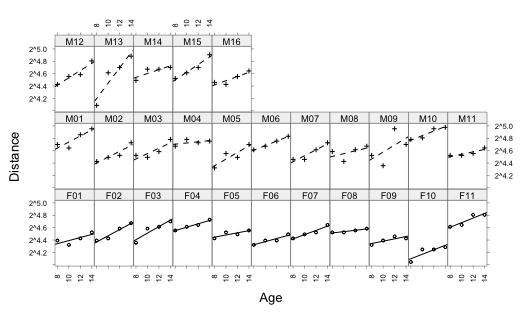
\includegraphics[width=1\textwidth,height=\textheight]{figs/g7_14-1.png}
\end{center}

\begin{Shaded}
\begin{Highlighting}[]
\DocumentationTok{\#\# Plot showing pattern of change for each of the 25 individuals}
\NormalTok{gph }\OtherTok{\textless{}{-}} \FunctionTok{xyplot}\NormalTok{(distance }\SpecialCharTok{\textasciitilde{}}\NormalTok{ age }\SpecialCharTok{|}\NormalTok{ Subject, }\AttributeTok{groups=}\NormalTok{Sex, }\AttributeTok{data=}\NormalTok{Orthodont,}
              \AttributeTok{scales=}\FunctionTok{list}\NormalTok{(}\AttributeTok{x=}\FunctionTok{list}\NormalTok{(}\AttributeTok{rot=}\DecValTok{90}\NormalTok{, }\AttributeTok{tick.number=}\DecValTok{3}\NormalTok{), }\AttributeTok{y=}\FunctionTok{list}\NormalTok{(}\AttributeTok{log=}\DecValTok{2}\NormalTok{), }\AttributeTok{tck=}\FloatTok{0.5}\NormalTok{), }\AttributeTok{type=}\FunctionTok{c}\NormalTok{(}\StringTok{"p"}\NormalTok{,}\StringTok{"r"}\NormalTok{),}
              \AttributeTok{layout=}\FunctionTok{c}\NormalTok{(}\DecValTok{11}\NormalTok{,}\DecValTok{3}\NormalTok{))}
\FunctionTok{update}\NormalTok{(gph, }\AttributeTok{xlab=}\FunctionTok{list}\NormalTok{(}\StringTok{"Age"}\NormalTok{, }\AttributeTok{cex=}\FloatTok{1.4}\NormalTok{), }\AttributeTok{ylab=}\FunctionTok{list}\NormalTok{(}\StringTok{"Distance"}\NormalTok{, }\AttributeTok{cex=}\FloatTok{1.4}\NormalTok{),}
       \AttributeTok{par.settings=}\NormalTok{DAAG}\SpecialCharTok{::}\FunctionTok{DAAGtheme}\NormalTok{(}\AttributeTok{color=}\ConstantTok{FALSE}\NormalTok{, }\AttributeTok{fontsize=}\FunctionTok{list}\NormalTok{(}\AttributeTok{text=}\DecValTok{7}\NormalTok{, }\AttributeTok{points=}\DecValTok{4}\NormalTok{)))}
\end{Highlighting}
\end{Shaded}

\paragraph{Preliminary data
exploration}\label{preliminary-data-exploration}

\begin{Shaded}
\begin{Highlighting}[]
\DocumentationTok{\#\# Use lmList() to find the slopes}
\NormalTok{ab }\OtherTok{\textless{}{-}} \FunctionTok{cbind}\NormalTok{(}\FunctionTok{coef}\NormalTok{(}\FunctionTok{lmList}\NormalTok{(distance }\SpecialCharTok{\textasciitilde{}}\NormalTok{ age }\SpecialCharTok{|}\NormalTok{ Subject, Orthodont)),}
            \FunctionTok{coef}\NormalTok{(}\FunctionTok{lmList}\NormalTok{(logdist }\SpecialCharTok{\textasciitilde{}}\NormalTok{ age}\SpecialCharTok{|}\NormalTok{Subject, }\AttributeTok{data=}\NormalTok{Orthodont)))}
\FunctionTok{names}\NormalTok{(ab) }\OtherTok{\textless{}{-}} \FunctionTok{c}\NormalTok{(}\StringTok{"a"}\NormalTok{, }\StringTok{"b"}\NormalTok{,}\StringTok{"alog"}\NormalTok{,}\StringTok{"blog"}\NormalTok{)}
\DocumentationTok{\#\# Obtain intercept at x=mean(x)=11, for each subject.}
\DocumentationTok{\#\# (For each subject, this is independent of the slope)}
\NormalTok{ab }\OtherTok{\textless{}{-}} \FunctionTok{within}\NormalTok{(ab, \{ybar }\OtherTok{=}\NormalTok{ a }\SpecialCharTok{+}\NormalTok{ b}\SpecialCharTok{*}\DecValTok{11}\NormalTok{; b}\OtherTok{=}\NormalTok{b; ylogbar }\OtherTok{=}\NormalTok{ alog }\SpecialCharTok{+}\NormalTok{ blog }\SpecialCharTok{*} \DecValTok{11}\NormalTok{;}
\NormalTok{                  blog}\OtherTok{=}\NormalTok{blog; sex }\OtherTok{=} \FunctionTok{substring}\NormalTok{(}\FunctionTok{rownames}\NormalTok{(ab), }\DecValTok{1}\NormalTok{ ,}\DecValTok{1}\NormalTok{)}
\NormalTok{                  \})}
\NormalTok{bySex }\OtherTok{\textless{}{-}} \FunctionTok{sapply}\NormalTok{(}\FunctionTok{split}\NormalTok{(ab, ab}\SpecialCharTok{$}\NormalTok{sex), }\ControlFlowTok{function}\NormalTok{(z)}\FunctionTok{range}\NormalTok{(z}\SpecialCharTok{$}\NormalTok{b))}
\NormalTok{extremes }\OtherTok{\textless{}{-}} \FunctionTok{with}\NormalTok{(ab, ybar }\SpecialCharTok{\%in\%} \FunctionTok{range}\NormalTok{(ybar) }\SpecialCharTok{|}\NormalTok{ b }\SpecialCharTok{\%in\%}\NormalTok{ bySex)}
\end{Highlighting}
\end{Shaded}

\begin{center}
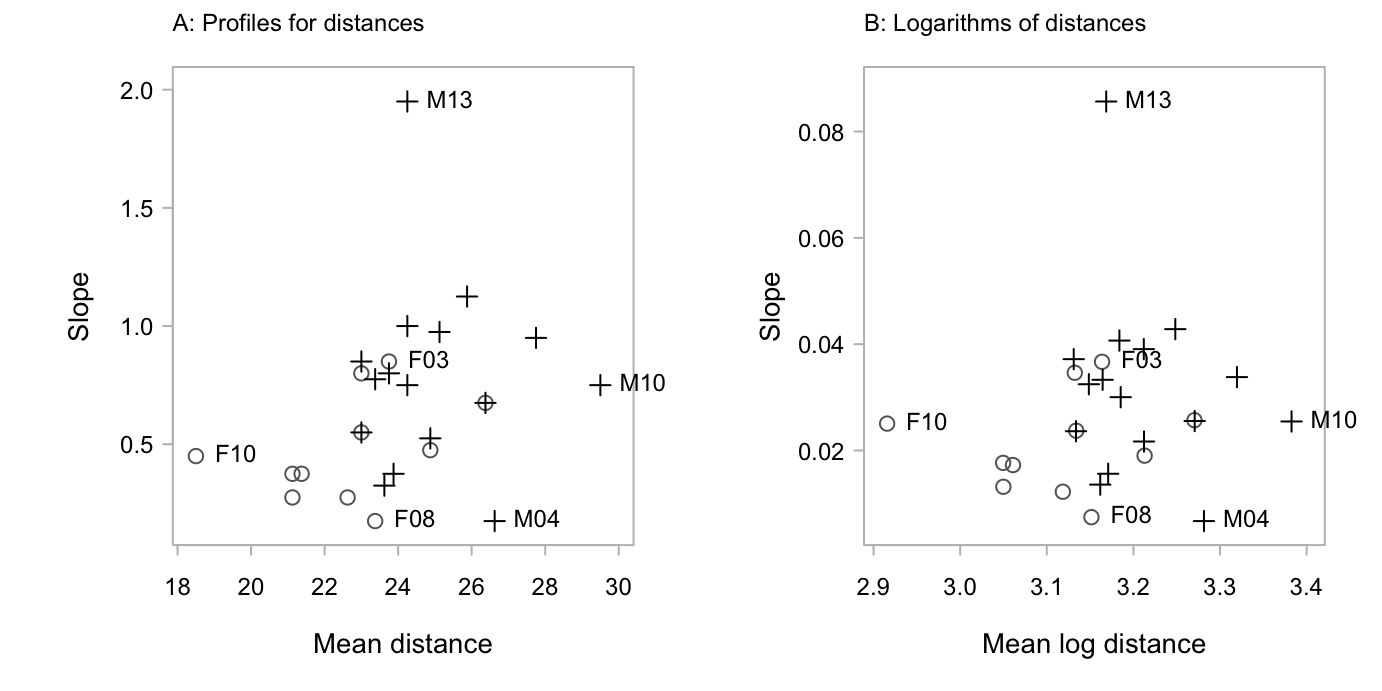
\includegraphics[width=1\textwidth,height=\textheight]{figs/g7_15-1.png}
\end{center}

\begin{Shaded}
\begin{Highlighting}[]
\NormalTok{fundiff }\OtherTok{\textless{}{-}} \ControlFlowTok{function}\NormalTok{(x)}\FunctionTok{range}\NormalTok{(x)}\SpecialCharTok{+}\FunctionTok{diff}\NormalTok{(}\FunctionTok{range}\NormalTok{(x))}\SpecialCharTok{*}\FunctionTok{c}\NormalTok{(}\SpecialCharTok{{-}}\FloatTok{0.015}\NormalTok{, }\FloatTok{0.04}\NormalTok{)}
\NormalTok{lims }\OtherTok{\textless{}{-}} \FunctionTok{sapply}\NormalTok{(}\FunctionTok{subset}\NormalTok{(ab, }\AttributeTok{select=}\FunctionTok{c}\NormalTok{(}\StringTok{\textquotesingle{}ybar\textquotesingle{}}\NormalTok{,}\StringTok{"b"}\NormalTok{,}\StringTok{"ylogbar"}\NormalTok{,}\StringTok{"blog"}\NormalTok{)), fundiff)}
\FunctionTok{plot}\NormalTok{(b }\SpecialCharTok{\textasciitilde{}}\NormalTok{ ybar, }\AttributeTok{col=}\FunctionTok{c}\NormalTok{(}\AttributeTok{F=}\StringTok{"gray40"}\NormalTok{, }\AttributeTok{M=}\StringTok{"black"}\NormalTok{)[sex], }\AttributeTok{data=}\NormalTok{ab,}
     \AttributeTok{fg=}\StringTok{"gray"}\NormalTok{, }\AttributeTok{xlim=}\NormalTok{lims[,}\StringTok{"ybar"}\NormalTok{], }\AttributeTok{ylim=}\NormalTok{lims[,}\StringTok{"b"}\NormalTok{],}
     \AttributeTok{pch=}\FunctionTok{c}\NormalTok{(}\AttributeTok{F=}\DecValTok{1}\NormalTok{, }\AttributeTok{M=}\DecValTok{3}\NormalTok{)[sex], }\AttributeTok{xlab=}\StringTok{"Mean distance"}\NormalTok{, }\AttributeTok{ylab=}\StringTok{"Slope"}\NormalTok{)}
\FunctionTok{with}\NormalTok{(}\FunctionTok{subset}\NormalTok{(ab, extremes), }\FunctionTok{text}\NormalTok{(b }\SpecialCharTok{\textasciitilde{}}\NormalTok{ ybar,}
    \AttributeTok{labels=}\FunctionTok{rownames}\NormalTok{(ab)[extremes], }\AttributeTok{pos=}\DecValTok{4}\NormalTok{, }\AttributeTok{xpd=}\ConstantTok{TRUE}\NormalTok{))}
\FunctionTok{mtext}\NormalTok{(}\AttributeTok{side=}\DecValTok{3}\NormalTok{, }\AttributeTok{line=}\FloatTok{0.75}\NormalTok{,}\StringTok{"A: Profiles for distances"}\NormalTok{, }\AttributeTok{adj=}\DecValTok{0}\NormalTok{)}
\CommentTok{\# Type \textquotesingle{}qqnorm(ab$b)\textquotesingle{} to see the extent of M13\textquotesingle{}s outlyingness}
\DocumentationTok{\#\# For Panel B, repeat with logdist replacing distance}
\FunctionTok{plot}\NormalTok{(blog }\SpecialCharTok{\textasciitilde{}}\NormalTok{ ylogbar, }\AttributeTok{col=}\FunctionTok{c}\NormalTok{(}\AttributeTok{F=}\StringTok{"gray40"}\NormalTok{, }\AttributeTok{M=}\StringTok{"black"}\NormalTok{)[sex], }\AttributeTok{data=}\NormalTok{ab, }\AttributeTok{fg=}\StringTok{"gray"}\NormalTok{,}
     \AttributeTok{pch=}\FunctionTok{c}\NormalTok{(}\AttributeTok{F=}\DecValTok{1}\NormalTok{, }\AttributeTok{M=}\DecValTok{3}\NormalTok{)[sex], }\AttributeTok{xlim=}\NormalTok{lims[,}\StringTok{"ylogbar"}\NormalTok{], }\AttributeTok{ylim=}\NormalTok{lims[,}\StringTok{"blog"}\NormalTok{],}
     \AttributeTok{xlab=}\StringTok{"Mean log distance"}\NormalTok{, }\AttributeTok{ylab=}\StringTok{"Slope"}\NormalTok{)}
\FunctionTok{with}\NormalTok{(}\FunctionTok{subset}\NormalTok{(ab, extremes),}
     \FunctionTok{text}\NormalTok{(blog }\SpecialCharTok{\textasciitilde{}}\NormalTok{ ylogbar, }\AttributeTok{labels=}\FunctionTok{rownames}\NormalTok{(ab)[extremes], }\AttributeTok{pos=}\DecValTok{4}\NormalTok{, }\AttributeTok{xpd=}\ConstantTok{TRUE}\NormalTok{))}
\FunctionTok{mtext}\NormalTok{(}\AttributeTok{side=}\DecValTok{3}\NormalTok{, }\AttributeTok{line=}\FloatTok{0.75}\NormalTok{,}\StringTok{"B: Logarithms of distances"}\NormalTok{, }\AttributeTok{adj=}\DecValTok{0}\NormalTok{)}
\end{Highlighting}
\end{Shaded}

\begin{Shaded}
\begin{Highlighting}[]
\DocumentationTok{\#\# Compare male slopes with female slopes}
\NormalTok{extreme.males }\OtherTok{\textless{}{-}} \FunctionTok{match}\NormalTok{(}\FunctionTok{c}\NormalTok{(}\StringTok{"M04"}\NormalTok{,}\StringTok{"M13"}\NormalTok{), }\FunctionTok{rownames}\NormalTok{(ab))}
\FunctionTok{with}\NormalTok{(ab[}\SpecialCharTok{{-}}\NormalTok{extreme.males,],}
\FunctionTok{t.test}\NormalTok{(blog[sex}\SpecialCharTok{==}\StringTok{"F"}\NormalTok{], blog[sex}\SpecialCharTok{==}\StringTok{"M"}\NormalTok{], }\AttributeTok{var.equal=}\ConstantTok{TRUE}\NormalTok{))}
\end{Highlighting}
\end{Shaded}

\begin{verbatim}

    Two Sample t-test

data:  blog[sex == "F"] and blog[sex == "M"]
t = -2.3, df = 23, p-value = 0.03
alternative hypothesis: true difference in means is not equal to 0
95 percent confidence interval:
 -0.0160529 -0.0009191
sample estimates:
mean of x mean of y 
  0.02115   0.02963 
\end{verbatim}

\begin{Shaded}
\begin{Highlighting}[]
\CommentTok{\# Specify var.equal=TRUE, to allow comparison with anova output}
\end{Highlighting}
\end{Shaded}

\paragraph{A random coefficients
model}\label{a-random-coefficients-model-1}

\begin{Shaded}
\begin{Highlighting}[]
\NormalTok{keep }\OtherTok{\textless{}{-}} \SpecialCharTok{!}\NormalTok{(Orthodont}\SpecialCharTok{$}\NormalTok{Subject}\SpecialCharTok{\%in\%}\FunctionTok{c}\NormalTok{(}\StringTok{"M04"}\NormalTok{,}\StringTok{"M13"}\NormalTok{))}
\NormalTok{Orthodont}\SpecialCharTok{$}\NormalTok{scAge }\OtherTok{\textless{}{-}} \FunctionTok{with}\NormalTok{(Orthodont, age}\DecValTok{{-}11}\NormalTok{)  }\DocumentationTok{\#\# Center values of age}
\NormalTok{orthdiffx.lmer }\OtherTok{\textless{}{-}} \FunctionTok{lmer}\NormalTok{(logdist }\SpecialCharTok{\textasciitilde{}}\NormalTok{ Sex }\SpecialCharTok{*}\NormalTok{ scAge }\SpecialCharTok{+}\NormalTok{ (scAge }\SpecialCharTok{|}\NormalTok{ Subject),}
                       \AttributeTok{data=}\NormalTok{Orthodont, }\AttributeTok{subset=}\NormalTok{keep)}
\end{Highlighting}
\end{Shaded}

\begin{Shaded}
\begin{Highlighting}[]
\FunctionTok{rePCA}\NormalTok{(orthdiffx.lmer)}
\end{Highlighting}
\end{Shaded}

\begin{verbatim}
$Subject
Standard deviations (1, .., p=2):
[1] 1.632 0.000

Rotation (n x k) = (2 x 2):
         [,1]     [,2]
[1,] -0.99993 -0.01153
[2,] -0.01153  0.99993

attr(,"class")
[1] "prcomplist"
\end{verbatim}

\begin{Shaded}
\begin{Highlighting}[]
\NormalTok{orthdiff.lmer }\OtherTok{\textless{}{-}} \FunctionTok{lmer}\NormalTok{(logdist }\SpecialCharTok{\textasciitilde{}}\NormalTok{ Sex }\SpecialCharTok{*}\NormalTok{ scAge }\SpecialCharTok{+}\NormalTok{ (}\DecValTok{1} \SpecialCharTok{|}\NormalTok{ Subject),}
                      \AttributeTok{data=}\NormalTok{Orthodont, }\AttributeTok{subset=}\NormalTok{keep)}
\FunctionTok{summary}\NormalTok{(orthdiff.lmer)}
\end{Highlighting}
\end{Shaded}

\begin{verbatim}
Linear mixed model fit by REML ['lmerMod']
Formula: logdist ~ Sex * scAge + (1 | Subject)
   Data: Orthodont
 Subset: keep

REML criterion at convergence: -232

Scaled residuals: 
   Min     1Q Median     3Q    Max 
-3.312 -0.510  0.014  0.543  3.945 

Random effects:
 Groups   Name        Variance Std.Dev.
 Subject  (Intercept) 0.00633  0.0796  
 Residual             0.00238  0.0488  
Number of obs: 100, groups:  Subject, 25

Fixed effects:
              Estimate Std. Error t value
(Intercept)    3.11451    0.02510  124.11
SexMale        0.09443    0.03354    2.82
scAge          0.02115    0.00329    6.42
SexMale:scAge  0.00849    0.00440    1.93

Correlation of Fixed Effects:
            (Intr) SexMal scAge 
SexMale     -0.748              
scAge        0.000  0.000       
SexMal:scAg  0.000  0.000 -0.748
\end{verbatim}

\begin{Shaded}
\begin{Highlighting}[]
\NormalTok{Orthodont2 }\OtherTok{\textless{}{-}} \FunctionTok{droplevels}\NormalTok{(}\FunctionTok{subset}\NormalTok{(Orthodont, keep))}
\NormalTok{opt }\OtherTok{\textless{}{-}} \FunctionTok{options}\NormalTok{(}\AttributeTok{contrasts=}\FunctionTok{c}\NormalTok{(}\StringTok{"contr.sum"}\NormalTok{,}\StringTok{"contr.poly"}\NormalTok{))}
\NormalTok{orthdiff.mixed }\OtherTok{\textless{}{-}}\NormalTok{ afex}\SpecialCharTok{::}\FunctionTok{mixed}\NormalTok{(logdist }\SpecialCharTok{\textasciitilde{}}\NormalTok{ Sex }\SpecialCharTok{*}\NormalTok{ scAge }\SpecialCharTok{+}\NormalTok{ (}\DecValTok{1} \SpecialCharTok{|}\NormalTok{ Subject), }\AttributeTok{type=}\DecValTok{2}\NormalTok{,}
                              \AttributeTok{method=}\StringTok{\textquotesingle{}S\textquotesingle{}}\NormalTok{, }\AttributeTok{data=}\NormalTok{Orthodont2)}
  \DocumentationTok{\#\# NB \textasciigrave{}type\textasciigrave{} refers to type of test, NOT \textasciigrave{}error\textasciigrave{} type.}
\FunctionTok{options}\NormalTok{(opt)       }\CommentTok{\# Reset to previous contrasts setting}
\NormalTok{orthdiff.mixed}
\end{Highlighting}
\end{Shaded}

\begin{verbatim}
Mixed Model Anova Table (Type 2 tests, S-method)

Model: logdist ~ Sex * scAge + (1 | Subject)
Data: Orthodont2
     Effect       df          F p.value
1       Sex 1, 23.00    7.93 **    .010
2     scAge 1, 73.00 140.72 ***   <.001
3 Sex:scAge 1, 73.00     3.72 +    .058
---
Signif. codes:  0 '***' 0.001 '**' 0.01 '*' 0.05 '+' 0.1 ' ' 1
\end{verbatim}

\begin{Shaded}
\begin{Highlighting}[]
\FunctionTok{contrasts}\NormalTok{(Orthodont2[[}\StringTok{\textquotesingle{}Subject\textquotesingle{}}\NormalTok{]]) }\OtherTok{\textless{}{-}} \StringTok{\textquotesingle{}contr.sum\textquotesingle{}}
\FunctionTok{contrasts}\NormalTok{(Orthodont2[[}\StringTok{\textquotesingle{}Sex\textquotesingle{}}\NormalTok{]]) }\OtherTok{\textless{}{-}} \StringTok{\textquotesingle{}contr.sum\textquotesingle{}}
\end{Highlighting}
\end{Shaded}

\begin{Shaded}
\begin{Highlighting}[]
\NormalTok{orthdiffa.lmer }\OtherTok{\textless{}{-}} \FunctionTok{update}\NormalTok{(orthdiff.lmer, }\AttributeTok{formula=}\NormalTok{. }\SpecialCharTok{\textasciitilde{}}\NormalTok{ . }\SpecialCharTok{{-}}\NormalTok{Sex}\SpecialCharTok{:}\NormalTok{scAge)}
\FunctionTok{AIC}\NormalTok{(orthdiffa.lmer,orthdiff.lmer)}
\end{Highlighting}
\end{Shaded}

\begin{verbatim}
               df    AIC
orthdiffa.lmer  5 -227.4
orthdiff.lmer   6 -220.1
\end{verbatim}

\paragraph{Correlation between successive
times}\label{correlation-between-successive-times}

\begin{Shaded}
\begin{Highlighting}[]
\NormalTok{res }\OtherTok{\textless{}{-}} \FunctionTok{resid}\NormalTok{(orthdiff.lmer)}
\NormalTok{Subject }\OtherTok{\textless{}{-}} \FunctionTok{factor}\NormalTok{(Orthodont}\SpecialCharTok{$}\NormalTok{Subject[keep])}
\NormalTok{orth.arma }\OtherTok{\textless{}{-}} \FunctionTok{sapply}\NormalTok{(}\FunctionTok{split}\NormalTok{(res, Subject),}
                    \ControlFlowTok{function}\NormalTok{(x)forecast}\SpecialCharTok{::}\FunctionTok{auto.arima}\NormalTok{(x)}\SpecialCharTok{$}\NormalTok{arma[}\FunctionTok{c}\NormalTok{(}\DecValTok{1}\NormalTok{,}\DecValTok{6}\NormalTok{,}\DecValTok{2}\NormalTok{)])}
\end{Highlighting}
\end{Shaded}

\begin{Shaded}
\begin{Highlighting}[]
\NormalTok{orthsum }\OtherTok{\textless{}{-}} \FunctionTok{apply}\NormalTok{(orth.arma,}\DecValTok{2}\NormalTok{,sum)}
\NormalTok{orth.arma[, orthsum}\SpecialCharTok{\textgreater{}}\DecValTok{0}\NormalTok{]}
\end{Highlighting}
\end{Shaded}

\begin{verbatim}
     F08 M06
[1,]   1   1
[2,]   0   0
[3,]   1   1
\end{verbatim}

\paragraph{Fitting a sequential correlation
structure}\label{fitting-a-sequential-correlation-structure}

\begin{Shaded}
\begin{Highlighting}[]
\FunctionTok{library}\NormalTok{(nlme)}
\NormalTok{keep }\OtherTok{\textless{}{-}} \SpecialCharTok{!}\NormalTok{(Orthodont}\SpecialCharTok{$}\NormalTok{Subject}\SpecialCharTok{\%in\%}\FunctionTok{c}\NormalTok{(}\StringTok{"M04"}\NormalTok{,}\StringTok{"M13"}\NormalTok{))}
\NormalTok{Orthodont2 }\OtherTok{\textless{}{-}} \FunctionTok{droplevels}\NormalTok{(}\FunctionTok{subset}\NormalTok{(Orthodont,keep))}
\NormalTok{orthdiff.lme }\OtherTok{\textless{}{-}} \FunctionTok{lme}\NormalTok{(logdist }\SpecialCharTok{\textasciitilde{}}\NormalTok{ Sex }\SpecialCharTok{*}\NormalTok{ scAge, }\AttributeTok{random =} \SpecialCharTok{\textasciitilde{}}\DecValTok{1}\SpecialCharTok{|}\NormalTok{Subject,}
                    \AttributeTok{cor=}\FunctionTok{corCAR1}\NormalTok{(}\FloatTok{0.1}\NormalTok{, }\AttributeTok{form=}\SpecialCharTok{\textasciitilde{}}\DecValTok{1}\SpecialCharTok{|}\NormalTok{Subject), }\AttributeTok{data=}\NormalTok{Orthodont2)}
\DocumentationTok{\#\# For AR1 models \textasciigrave{}phi\textasciigrave{} is the sequential correlation estimate}
\NormalTok{orthdiff.lme}\SpecialCharTok{$}\NormalTok{modelStruct}\SpecialCharTok{$}\NormalTok{corStruct}
\end{Highlighting}
\end{Shaded}

\begin{verbatim}
Correlation structure of class corCAR1 representing
            Phi 
0.0000000003311 
\end{verbatim}

\paragraph{*The variance for the difference in
slopes}\label{the-variance-for-the-difference-in-slopes}

\subsection{Section 7.9: Further notes on multilevel
models}\label{section-7.9-further-notes-on-multilevel-models}

\subsubsection{Subsection 7.9.1: Sources of variation -- complication or
focus of
interest?}\label{subsection-7.9.1-sources-of-variation-complication-or-focus-of-interest}

\subsubsection{Subsection 7.9.2: Predictions from models with a complex
error
structure}\label{subsection-7.9.2-predictions-from-models-with-a-complex-error-structure}

\paragraph{Consequences from assuming an overly simplistic error
structure}\label{consequences-from-assuming-an-overly-simplistic-error-structure}

\subsubsection{Subsection 7.9.3: An historical perspective on multilevel
models}\label{subsection-7.9.3-an-historical-perspective-on-multilevel-models}

\subsubsection{Subsection 7.9.4:
Meta-analysis}\label{subsection-7.9.4-meta-analysis}

\subsubsection{Subsection 7.9.5: Functional data
analysis}\label{subsection-7.9.5-functional-data-analysis}

\subsubsection{Subsection 7.9.6: Error structure in explanatory
variables}\label{subsection-7.9.6-error-structure-in-explanatory-variables}

\subsection{Exercises (7.12)}\label{exercises-7.12}

7.1

\begin{Shaded}
\begin{Highlighting}[]
\NormalTok{n.omit }\OtherTok{\textless{}{-}} \DecValTok{2}
\NormalTok{take }\OtherTok{\textless{}{-}} \FunctionTok{rep}\NormalTok{(}\ConstantTok{TRUE}\NormalTok{, }\DecValTok{48}\NormalTok{)}
\NormalTok{take[}\FunctionTok{sample}\NormalTok{(}\DecValTok{1}\SpecialCharTok{:}\DecValTok{48}\NormalTok{,}\DecValTok{2}\NormalTok{)] }\OtherTok{\textless{}{-}} \ConstantTok{FALSE}
\NormalTok{kiwishade.lmer }\OtherTok{\textless{}{-}} \FunctionTok{lmer}\NormalTok{(yield }\SpecialCharTok{\textasciitilde{}}\NormalTok{ shade }\SpecialCharTok{+}\NormalTok{ (}\DecValTok{1}\SpecialCharTok{|}\NormalTok{block) }\SpecialCharTok{+}\NormalTok{ (}\DecValTok{1}\SpecialCharTok{|}\NormalTok{block}\SpecialCharTok{:}\NormalTok{plot),}
                       \AttributeTok{data =}\NormalTok{ kiwishade,}\AttributeTok{subset=}\NormalTok{take)}
\NormalTok{vcov }\OtherTok{\textless{}{-}} \FunctionTok{VarCorr}\NormalTok{(kiwishade.lmer)}
\FunctionTok{print}\NormalTok{(vcov, }\AttributeTok{comp=}\StringTok{"Variance"}\NormalTok{)}
\end{Highlighting}
\end{Shaded}

\begin{verbatim}
 Groups     Name        Variance
 block:plot (Intercept)  2.35   
 block      (Intercept)  3.28   
 Residual               12.45   
\end{verbatim}

7.6

\begin{Shaded}
\begin{Highlighting}[]
\NormalTok{cult.lmer }\OtherTok{\textless{}{-}} \FunctionTok{lmer}\NormalTok{(ct }\SpecialCharTok{\textasciitilde{}}\NormalTok{ Cultivar }\SpecialCharTok{+}\NormalTok{ Dose }\SpecialCharTok{+} \FunctionTok{factor}\NormalTok{(year) }\SpecialCharTok{+}
\NormalTok{                       (}\SpecialCharTok{{-}}\DecValTok{1} \SpecialCharTok{+}\NormalTok{ Dose }\SpecialCharTok{|}\NormalTok{ gp), }\AttributeTok{data =}\NormalTok{ DAAG}\SpecialCharTok{::}\NormalTok{sorption, }\AttributeTok{REML=}\ConstantTok{TRUE}\NormalTok{)}
\NormalTok{cultdose.lmer }\OtherTok{\textless{}{-}} \FunctionTok{lmer}\NormalTok{(ct }\SpecialCharTok{\textasciitilde{}}\NormalTok{ Cultivar}\SpecialCharTok{/}\NormalTok{Dose }\SpecialCharTok{+} \FunctionTok{factor}\NormalTok{(year) }\SpecialCharTok{+}
\NormalTok{                           (}\SpecialCharTok{{-}}\DecValTok{1} \SpecialCharTok{+}\NormalTok{ Dose }\SpecialCharTok{|}\NormalTok{ gp), }\AttributeTok{data =}\NormalTok{ DAAG}\SpecialCharTok{::}\NormalTok{sorption, }\AttributeTok{REML=}\ConstantTok{TRUE}\NormalTok{)}
\end{Highlighting}
\end{Shaded}

\begin{Shaded}
\begin{Highlighting}[]
\ControlFlowTok{if}\NormalTok{(}\FunctionTok{file.exists}\NormalTok{(}\StringTok{"/Users/johnm1/pkgs/PGRcode/inst/doc/"}\NormalTok{))\{}
\NormalTok{code }\OtherTok{\textless{}{-}}\NormalTok{ knitr}\SpecialCharTok{::}\NormalTok{knit\_code}\SpecialCharTok{$}\FunctionTok{get}\NormalTok{()}
\NormalTok{txt }\OtherTok{\textless{}{-}} \FunctionTok{paste0}\NormalTok{(}\StringTok{"}\SpecialCharTok{\textbackslash{}n}\StringTok{\#\# "}\NormalTok{, }\FunctionTok{names}\NormalTok{(code),}\StringTok{"}\SpecialCharTok{\textbackslash{}n}\StringTok{"}\NormalTok{, }\FunctionTok{sapply}\NormalTok{(code, paste, }\AttributeTok{collapse=}\StringTok{\textquotesingle{}}\SpecialCharTok{\textbackslash{}n}\StringTok{\textquotesingle{}}\NormalTok{))}
\FunctionTok{writeLines}\NormalTok{(txt, }\AttributeTok{con=}\StringTok{"/Users/johnm1/pkgs/PGRcode/inst/doc/ch7.R"}\NormalTok{)}
\NormalTok{\}}
\end{Highlighting}
\end{Shaded}

\bookmarksetup{startatroot}

\chapter{Chapter 8: Tree-based Classification and
Regression}\label{chapter-8-tree-based-classification-and-regression}

\paragraph{Packages required (plus any
dependencies)}\label{packages-required-plus-any-dependencies-5}

DAAG latticeExtra plot rpart rpart.plot MASS ggplot2 car randomForest

Additionally, knitr and Hmisc are required in order to process the Rmd
source file.

\begin{Shaded}
\begin{Highlighting}[]
\NormalTok{Hmisc}\SpecialCharTok{::}\FunctionTok{knitrSet}\NormalTok{(}\AttributeTok{basename=}\StringTok{"treebased"}\NormalTok{, }\AttributeTok{lang=}\StringTok{\textquotesingle{}markdown\textquotesingle{}}\NormalTok{, }\AttributeTok{fig.path=}\StringTok{"figs/g"}\NormalTok{, }\AttributeTok{w=}\DecValTok{7}\NormalTok{, }\AttributeTok{h=}\DecValTok{7}\NormalTok{)}
\NormalTok{oldopt }\OtherTok{\textless{}{-}} \FunctionTok{options}\NormalTok{(}\AttributeTok{digits=}\DecValTok{4}\NormalTok{, }\AttributeTok{formatR.arrow=}\ConstantTok{FALSE}\NormalTok{, }\AttributeTok{width=}\DecValTok{70}\NormalTok{, }\AttributeTok{scipen=}\DecValTok{999}\NormalTok{)}
\FunctionTok{library}\NormalTok{(knitr)}
\DocumentationTok{\#\# knitr::render\_listings()}
\NormalTok{opts\_chunk[[}\StringTok{\textquotesingle{}set\textquotesingle{}}\NormalTok{]](}\AttributeTok{cache.path=}\StringTok{\textquotesingle{}cache{-}\textquotesingle{}}\NormalTok{, }\AttributeTok{out.width=}\StringTok{"80\%"}\NormalTok{, }\AttributeTok{fig.align=}\StringTok{"center"}\NormalTok{, }
                    \AttributeTok{fig.show=}\StringTok{\textquotesingle{}hold\textquotesingle{}}\NormalTok{, }\AttributeTok{size=}\StringTok{"small"}\NormalTok{, }\AttributeTok{ps=}\DecValTok{10}\NormalTok{, }\AttributeTok{strip.white =} \ConstantTok{TRUE}\NormalTok{,}
                    \AttributeTok{comment=}\ConstantTok{NA}\NormalTok{, }\AttributeTok{width=}\DecValTok{70}\NormalTok{, }\AttributeTok{tidy.opts =} \FunctionTok{list}\NormalTok{(}\AttributeTok{replace.assign=}\ConstantTok{FALSE}\NormalTok{))}
\end{Highlighting}
\end{Shaded}

\begin{Shaded}
\begin{Highlighting}[]
\FunctionTok{suppressPackageStartupMessages}\NormalTok{(}\FunctionTok{library}\NormalTok{(latticeExtra))}
\end{Highlighting}
\end{Shaded}

\paragraph{When are tree-based methods
appropriate?}\label{when-are-tree-based-methods-appropriate}

\subsection{Section 8.1: Tree-based methods --- uses and basic
notions}\label{section-8.1-tree-based-methods-uses-and-basic-notions}

\paragraph{Examples that will be used to demonstrate the
methodology}\label{examples-that-will-be-used-to-demonstrate-the-methodology}

\subsubsection{Subsection 8.1.1: Detecting email spam\textasciitilde--
an initial
look}\label{subsection-8.1.1-detecting-email-spam-an-initial-look}

\begin{center}
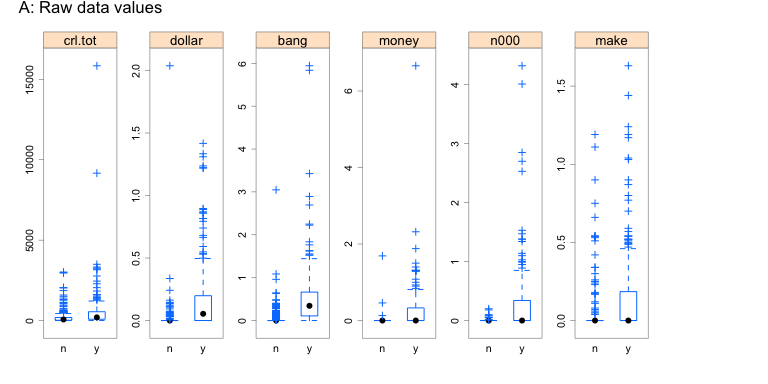
\includegraphics[width=1\textwidth,height=\textheight]{figs/g8_1-1.png}
\end{center}

\begin{center}
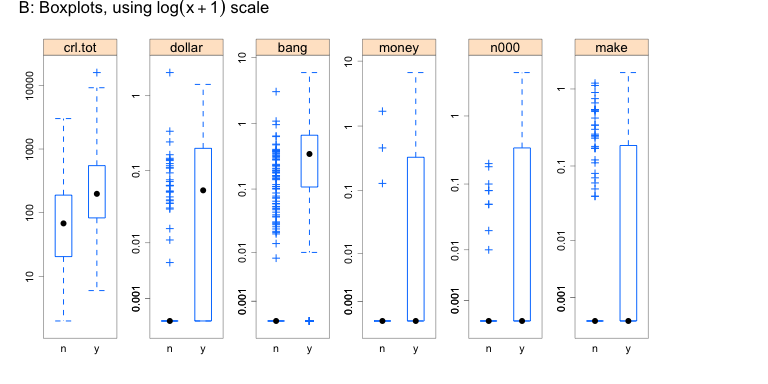
\includegraphics[width=1\textwidth,height=\textheight]{figs/g8_1-2.png}
\end{center}

\begin{Shaded}
\begin{Highlighting}[]
\NormalTok{nam }\OtherTok{\textless{}{-}} \FunctionTok{c}\NormalTok{(}\StringTok{"crl.tot"}\NormalTok{, }\StringTok{"dollar"}\NormalTok{, }\StringTok{"bang"}\NormalTok{, }\StringTok{"money"}\NormalTok{, }\StringTok{"n000"}\NormalTok{, }\StringTok{"make"}\NormalTok{)}
\NormalTok{nr }\OtherTok{\textless{}{-}} \FunctionTok{sample}\NormalTok{(}\DecValTok{1}\SpecialCharTok{:}\FunctionTok{dim}\NormalTok{(DAAG}\SpecialCharTok{::}\NormalTok{spam7)[}\DecValTok{1}\NormalTok{],}\DecValTok{500}\NormalTok{)}
\NormalTok{yesno}\OtherTok{\textless{}{-}}\NormalTok{DAAG}\SpecialCharTok{::}\NormalTok{spam7}\SpecialCharTok{$}\NormalTok{yesno[nr]}
\NormalTok{spam7a }\OtherTok{\textless{}{-}}\NormalTok{ DAAG}\SpecialCharTok{::}\NormalTok{spam7[nr,}\FunctionTok{c}\NormalTok{(nam,}\StringTok{"yesno"}\NormalTok{)]}
\NormalTok{formab }\OtherTok{\textless{}{-}} \FunctionTok{as.formula}\NormalTok{(}\FunctionTok{paste}\NormalTok{(}\FunctionTok{paste}\NormalTok{(nam, }\AttributeTok{collapse=}\StringTok{\textquotesingle{}+\textquotesingle{}}\NormalTok{), }\StringTok{\textquotesingle{}\textasciitilde{} yesno\textquotesingle{}}\NormalTok{))}
\NormalTok{spamtheme }\OtherTok{\textless{}{-}}\NormalTok{ DAAG}\SpecialCharTok{::}\FunctionTok{DAAGtheme}\NormalTok{(}\AttributeTok{color =} \ConstantTok{TRUE}\NormalTok{, }\AttributeTok{pch=}\DecValTok{3}\NormalTok{)}
\NormalTok{lattice}\SpecialCharTok{::}\FunctionTok{bwplot}\NormalTok{(formab, }\AttributeTok{data=}\NormalTok{spam7a, }\AttributeTok{outer=}\NormalTok{T, }\AttributeTok{horizontal=}\NormalTok{F, }\AttributeTok{layout=}\FunctionTok{c}\NormalTok{(}\DecValTok{7}\NormalTok{,}\DecValTok{1}\NormalTok{),}
  \AttributeTok{scales=}\FunctionTok{list}\NormalTok{(}\AttributeTok{relation=}\StringTok{\textquotesingle{}free\textquotesingle{}}\NormalTok{), }\AttributeTok{ylab=}\StringTok{""}\NormalTok{, }\AttributeTok{par.settings=}\NormalTok{spamtheme,}
  \AttributeTok{between=}\FunctionTok{list}\NormalTok{(}\AttributeTok{x=}\FloatTok{0.5}\NormalTok{),}
  \AttributeTok{main=}\FunctionTok{list}\NormalTok{(}\StringTok{"A: Raw data values"}\NormalTok{, }\AttributeTok{y=}\FloatTok{1.0}\NormalTok{, }\AttributeTok{font=}\DecValTok{1}\NormalTok{, }\AttributeTok{cex=}\FloatTok{1.25}\NormalTok{))}
\NormalTok{spam7b }\OtherTok{\textless{}{-}} \FunctionTok{cbind}\NormalTok{(}\FunctionTok{log}\NormalTok{(spam7a[,}\SpecialCharTok{{-}}\DecValTok{7}\NormalTok{]}\SpecialCharTok{+}\FloatTok{0.001}\NormalTok{), }\AttributeTok{yesno=}\NormalTok{spam7a[,}\DecValTok{7}\NormalTok{])}
\NormalTok{yval }\OtherTok{\textless{}{-}}\FunctionTok{c}\NormalTok{(}\FloatTok{0.001}\NormalTok{, }\FloatTok{0.001}\NormalTok{,}\FloatTok{0.01}\NormalTok{,}\FloatTok{0.1}\NormalTok{,}\DecValTok{1}\NormalTok{,}\DecValTok{10}\NormalTok{,}\DecValTok{100}\NormalTok{,}\DecValTok{1000}\NormalTok{,}\DecValTok{10000}\NormalTok{)}
\NormalTok{lattice}\SpecialCharTok{::}\FunctionTok{bwplot}\NormalTok{(formab, }\AttributeTok{data=}\NormalTok{spam7b, }\AttributeTok{outer=}\NormalTok{T, }\AttributeTok{horizontal=}\NormalTok{F, }\AttributeTok{layout=}\FunctionTok{c}\NormalTok{(}\DecValTok{7}\NormalTok{,}\DecValTok{1}\NormalTok{),}
                \AttributeTok{scales=}\FunctionTok{list}\NormalTok{(}\AttributeTok{relation=}\StringTok{\textquotesingle{}free\textquotesingle{}}\NormalTok{, }
                \AttributeTok{y=}\FunctionTok{list}\NormalTok{(}\AttributeTok{at=}\FunctionTok{log}\NormalTok{(yval}\FloatTok{+0.001}\NormalTok{), }\AttributeTok{labels=}\NormalTok{yval, }\AttributeTok{rot=}\DecValTok{90}\NormalTok{)),}
                \AttributeTok{ylab=}\StringTok{""}\NormalTok{, }\AttributeTok{par.settings=}\NormalTok{spamtheme, }\AttributeTok{between=}\FunctionTok{list}\NormalTok{(}\AttributeTok{x=}\FloatTok{0.5}\NormalTok{),}
\AttributeTok{main=}\FunctionTok{list}\NormalTok{(}\FunctionTok{expression}\NormalTok{(}\StringTok{"B: Boxplots, using "}\SpecialCharTok{*}\FunctionTok{log}\NormalTok{(x}\SpecialCharTok{+}\DecValTok{001}\NormalTok{)}\SpecialCharTok{*}\StringTok{" scale"}\NormalTok{),}
          \AttributeTok{y=}\FloatTok{1.0}\NormalTok{, }\AttributeTok{font=}\DecValTok{1}\NormalTok{, }\AttributeTok{cex=}\FloatTok{1.25}\NormalTok{))}
\end{Highlighting}
\end{Shaded}

\begin{Shaded}
\begin{Highlighting}[]
\DocumentationTok{\#\# Obtain 500{-}row sample; repeat the first plot (of crl.tot)}
\NormalTok{spam.sample }\OtherTok{\textless{}{-}}\NormalTok{ spam7[}\FunctionTok{sample}\NormalTok{(}\FunctionTok{seq}\NormalTok{(}\DecValTok{1}\NormalTok{,}\DecValTok{4601}\NormalTok{), }\DecValTok{500}\NormalTok{, }\AttributeTok{replace=}\ConstantTok{FALSE}\NormalTok{), ]}
\FunctionTok{boxplot}\NormalTok{(}\FunctionTok{split}\NormalTok{(spam.sample}\SpecialCharTok{$}\NormalTok{crl.tot, spam.sample}\SpecialCharTok{$}\NormalTok{yesno))}
\end{Highlighting}
\end{Shaded}

\begin{center}
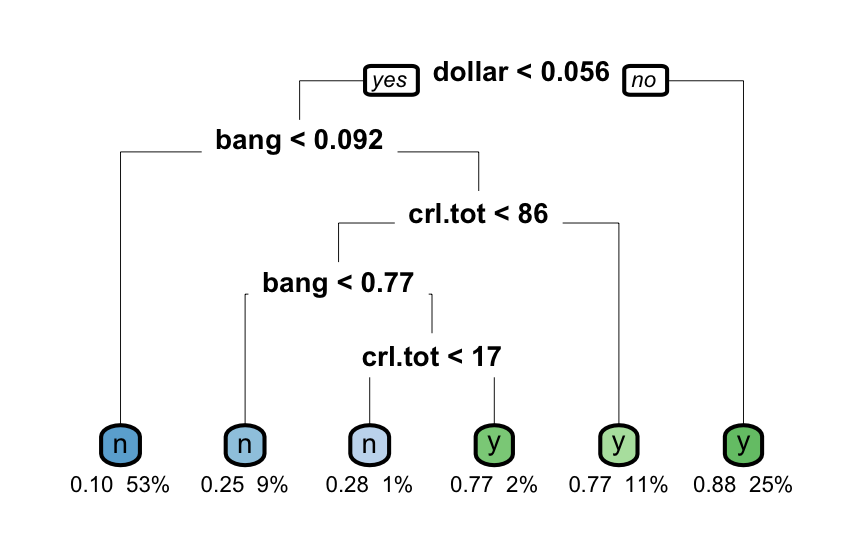
\includegraphics[width=0.65\textwidth,height=\textheight]{figs/g8_2-1.png}
\end{center}

\begin{Shaded}
\begin{Highlighting}[]
\FunctionTok{suppressMessages}\NormalTok{(}\FunctionTok{library}\NormalTok{(rpart))}
\FunctionTok{set.seed}\NormalTok{(}\DecValTok{31}\NormalTok{)      }\DocumentationTok{\#\# Reproduce tree shown in text}
\NormalTok{spam.rpart }\OtherTok{\textless{}{-}} \FunctionTok{rpart}\NormalTok{(}\AttributeTok{formula =}\NormalTok{ yesno }\SpecialCharTok{\textasciitilde{}}\NormalTok{ crl.tot }\SpecialCharTok{+}\NormalTok{ dollar }\SpecialCharTok{+}\NormalTok{ bang }\SpecialCharTok{+}\NormalTok{ money }\SpecialCharTok{+}\NormalTok{ n000 }\SpecialCharTok{+}
\NormalTok{                    make,  }\AttributeTok{method=}\StringTok{"class"}\NormalTok{, }\AttributeTok{model=}\ConstantTok{TRUE}\NormalTok{, }\AttributeTok{data=}\NormalTok{DAAG}\SpecialCharTok{::}\NormalTok{spam7)}
\NormalTok{rpart.plot}\SpecialCharTok{::}\FunctionTok{rpart.plot}\NormalTok{(spam.rpart, }\AttributeTok{type=}\DecValTok{0}\NormalTok{, }\AttributeTok{under=}\ConstantTok{TRUE}\NormalTok{, }\AttributeTok{branch.lwd=}\FloatTok{0.4}\NormalTok{,}
                       \AttributeTok{nn.lwd=}\FloatTok{0.4}\NormalTok{, }\AttributeTok{box.palette=}\StringTok{"auto"}\NormalTok{, }\AttributeTok{tweak=}\FloatTok{1.25}\NormalTok{)}
\end{Highlighting}
\end{Shaded}

\begin{Shaded}
\begin{Highlighting}[]
\FunctionTok{printcp}\NormalTok{(spam.rpart, }\AttributeTok{digits=}\DecValTok{3}\NormalTok{)}
\end{Highlighting}
\end{Shaded}

\begin{verbatim}

Classification tree:
rpart(formula = yesno ~ crl.tot + dollar + bang + money + n000 + 
    make, data = DAAG::spam7, method = "class", model = TRUE)

Variables actually used in tree construction:
[1] bang    crl.tot dollar 

Root node error: 1813/4601 = 0.394

n= 4601 

      CP nsplit rel error xerror   xstd
1 0.4766      0     1.000  1.000 0.0183
2 0.0756      1     0.523  0.547 0.0154
3 0.0116      3     0.372  0.388 0.0135
4 0.0105      4     0.361  0.384 0.0134
5 0.0100      5     0.350  0.382 0.0134
\end{verbatim}

\subsubsection{Subsection 8.1.2: Choosing the number of
splits}\label{subsection-8.1.2-choosing-the-number-of-splits}

\subsection{Section 8.2: Splitting criteria, with illustrative
examples}\label{section-8.2-splitting-criteria-with-illustrative-examples}

\begin{center}
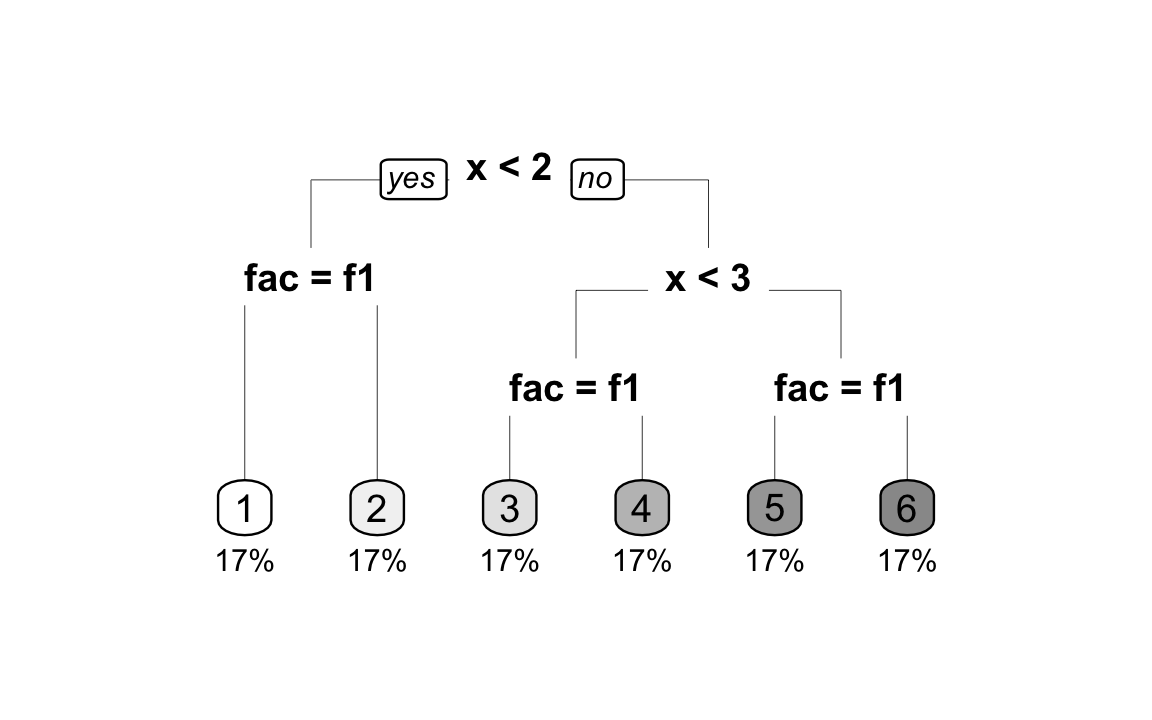
\includegraphics[width=0.8\textwidth,height=\textheight]{figs/g8_3-1.png}
\end{center}

\begin{Shaded}
\begin{Highlighting}[]
\NormalTok{tree.df }\OtherTok{\textless{}{-}} \FunctionTok{data.frame}\NormalTok{(}\AttributeTok{fac =} \FunctionTok{factor}\NormalTok{(}\FunctionTok{rep}\NormalTok{(}\FunctionTok{c}\NormalTok{(}\StringTok{\textquotesingle{}f1\textquotesingle{}}\NormalTok{,}\StringTok{\textquotesingle{}f2\textquotesingle{}}\NormalTok{), }\DecValTok{3}\NormalTok{)),}
\AttributeTok{x =} \FunctionTok{rep}\NormalTok{(}\DecValTok{1}\SpecialCharTok{:}\DecValTok{3}\NormalTok{, }\FunctionTok{rep}\NormalTok{(}\DecValTok{2}\NormalTok{, }\DecValTok{3}\NormalTok{)), }\AttributeTok{Node =} \DecValTok{1}\SpecialCharTok{:}\DecValTok{6}\NormalTok{)}
\NormalTok{u.tree }\OtherTok{\textless{}{-}} \FunctionTok{rpart}\NormalTok{(Node }\SpecialCharTok{\textasciitilde{}}\NormalTok{ fac }\SpecialCharTok{+}\NormalTok{ x, }\AttributeTok{data =}\NormalTok{ tree.df,}
                \AttributeTok{control =} \FunctionTok{list}\NormalTok{(}\AttributeTok{minsplit =} \DecValTok{2}\NormalTok{, }\AttributeTok{minbucket =} \DecValTok{1}\NormalTok{, }\AttributeTok{cp =} \FloatTok{1e{-}009}\NormalTok{))}
\NormalTok{rpart.plot}\SpecialCharTok{::}\FunctionTok{rpart.plot}\NormalTok{(u.tree, }\AttributeTok{type=}\DecValTok{0}\NormalTok{, }\AttributeTok{under=}\ConstantTok{TRUE}\NormalTok{, }\AttributeTok{branch.lwd=}\FloatTok{0.25}\NormalTok{,}
                       \AttributeTok{nn.lwd=}\FloatTok{0.25}\NormalTok{, }\AttributeTok{box.palette=}\StringTok{"Grays"}\NormalTok{, }\AttributeTok{tweak=}\FloatTok{1.6}\NormalTok{)}
\end{Highlighting}
\end{Shaded}

\paragraph{Choosing the split\textasciitilde-- regression
trees}\label{choosing-the-split-regression-trees}

\subsubsection{Subsection 8.2.1: Within and between sums of
squares}\label{subsection-8.2.1-within-and-between-sums-of-squares}

\subsubsection{Subsection 8.2.2: Choosing the split\textasciitilde--
classification
trees}\label{subsection-8.2.2-choosing-the-split-classification-trees}

\subsubsection{Subsection 8.2.3: Tree-based regression versus loess
regression
smoothing}\label{subsection-8.2.3-tree-based-regression-versus-loess-regression-smoothing}

\begin{center}
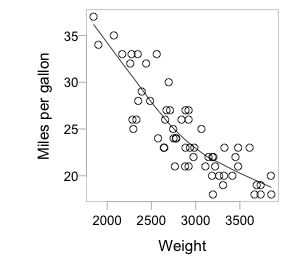
\includegraphics[width=0.4\textwidth,height=\textheight]{figs/g8_4-1.png}
\end{center}

\begin{Shaded}
\begin{Highlighting}[]
\NormalTok{u.lo }\OtherTok{\textless{}{-}} \FunctionTok{loess}\NormalTok{(Mileage}\SpecialCharTok{\textasciitilde{}}\NormalTok{Weight, }\AttributeTok{data =}\NormalTok{ car.test.frame, }\AttributeTok{span =} \DecValTok{2}\SpecialCharTok{/}\DecValTok{3}\NormalTok{)}
\FunctionTok{plot}\NormalTok{(Mileage}\SpecialCharTok{\textasciitilde{}}\NormalTok{Weight, }\AttributeTok{data=}\NormalTok{car.test.frame, }\AttributeTok{xlab =} \StringTok{"Weight"}\NormalTok{,}
     \AttributeTok{ylab =} \StringTok{"Miles per gallon"}\NormalTok{, }\AttributeTok{sub =} \StringTok{""}\NormalTok{, }\AttributeTok{fg=}\StringTok{"gray"}\NormalTok{)}
\NormalTok{xy }\OtherTok{\textless{}{-}} \FunctionTok{with}\NormalTok{(car.test.frame, }\FunctionTok{loess.smooth}\NormalTok{(Weight, Mileage))}
\NormalTok{ord}\OtherTok{\textless{}{-}}\FunctionTok{order}\NormalTok{(xy}\SpecialCharTok{$}\NormalTok{x)}
\FunctionTok{lines}\NormalTok{(xy}\SpecialCharTok{$}\NormalTok{x[ord],xy}\SpecialCharTok{$}\NormalTok{y[ord])}
\end{Highlighting}
\end{Shaded}

\begin{Shaded}
\begin{Highlighting}[]
\DocumentationTok{\#\# loess fit to Mileage vs Weight: data frame car.test.frame (rpart)}
\FunctionTok{with}\NormalTok{(rpart}\SpecialCharTok{::}\NormalTok{car.test.frame, }\FunctionTok{scatter.smooth}\NormalTok{(Mileage }\SpecialCharTok{\textasciitilde{}}\NormalTok{ Weight))}
\end{Highlighting}
\end{Shaded}

\begin{center}
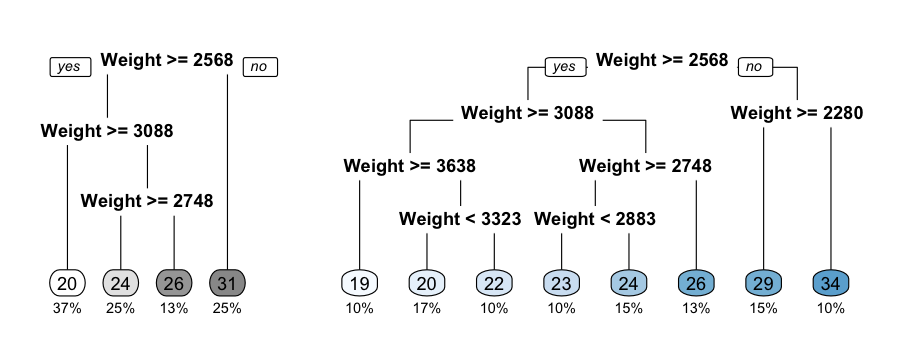
\includegraphics[width=1\textwidth,height=\textheight]{figs/g8_5-1.png}
\end{center}

\begin{Shaded}
\begin{Highlighting}[]
\FunctionTok{par}\NormalTok{(}\AttributeTok{fig=}\FunctionTok{c}\NormalTok{(}\DecValTok{0}\NormalTok{, }\FloatTok{0.32}\NormalTok{, }\DecValTok{0}\NormalTok{,}\DecValTok{1}\NormalTok{))}
\FunctionTok{set.seed}\NormalTok{(}\DecValTok{37}\NormalTok{)}
\NormalTok{car.tree }\OtherTok{\textless{}{-}} \FunctionTok{rpart}\NormalTok{(Mileage }\SpecialCharTok{\textasciitilde{}}\NormalTok{ Weight, }\AttributeTok{data =}\NormalTok{ car.test.frame)}
\NormalTok{rpart.plot}\SpecialCharTok{::}\FunctionTok{rpart.plot}\NormalTok{(car.tree, }\AttributeTok{type=}\DecValTok{0}\NormalTok{, }\AttributeTok{under=}\ConstantTok{TRUE}\NormalTok{,}
                       \AttributeTok{box.palette=}\StringTok{"Grays"}\NormalTok{, }\AttributeTok{tweak=}\FloatTok{1.05}\NormalTok{)}
\FunctionTok{par}\NormalTok{(}\AttributeTok{fig=}\FunctionTok{c}\NormalTok{(}\FloatTok{0.3}\NormalTok{,}\DecValTok{1}\NormalTok{, }\DecValTok{0}\NormalTok{,}\DecValTok{1}\NormalTok{), }\AttributeTok{new=}\ConstantTok{TRUE}\NormalTok{)}
\FunctionTok{set.seed}\NormalTok{(}\DecValTok{37}\NormalTok{)}
\NormalTok{car2.tree }\OtherTok{\textless{}{-}} \FunctionTok{rpart}\NormalTok{(Mileage}\SpecialCharTok{\textasciitilde{}}\NormalTok{Weight, }\AttributeTok{data=}\NormalTok{car.test.frame, }\AttributeTok{control =}
                   \FunctionTok{list}\NormalTok{(}\AttributeTok{minsplit =} \DecValTok{10}\NormalTok{, }\AttributeTok{minbucket =} \DecValTok{5}\NormalTok{, }\AttributeTok{cp =} \FloatTok{0.0001}\NormalTok{))}
\NormalTok{rpart.plot}\SpecialCharTok{::}\FunctionTok{rpart.plot}\NormalTok{(car2.tree, }\AttributeTok{type=}\DecValTok{0}\NormalTok{, }\AttributeTok{under=}\ConstantTok{TRUE}\NormalTok{,}
\AttributeTok{box.palette=}\StringTok{"auto"}\NormalTok{, }\AttributeTok{tweak=}\FloatTok{1.05}\NormalTok{)}
\end{Highlighting}
\end{Shaded}

\begin{Shaded}
\begin{Highlighting}[]
\DocumentationTok{\#\# Panel A: Split criteria were left a their defaults}
\NormalTok{car.tree }\OtherTok{\textless{}{-}} \FunctionTok{rpart}\NormalTok{(Mileage }\SpecialCharTok{\textasciitilde{}}\NormalTok{ Weight, }\AttributeTok{data =}\NormalTok{ car.test.frame)}
\NormalTok{rpart.plot}\SpecialCharTok{::}\FunctionTok{rpart.plot}\NormalTok{(car.tree, }\AttributeTok{type=}\DecValTok{0}\NormalTok{, }\AttributeTok{under=}\ConstantTok{TRUE}\NormalTok{)}
\DocumentationTok{\#\# Panel B: Finer grained splits}
\NormalTok{car2.tree }\OtherTok{\textless{}{-}} \FunctionTok{rpart}\NormalTok{(Mileage }\SpecialCharTok{\textasciitilde{}}\NormalTok{ Weight, }\AttributeTok{data=}\NormalTok{car.test.frame, }\AttributeTok{method=}\StringTok{"anova"}\NormalTok{,}
                   \AttributeTok{control =} \FunctionTok{list}\NormalTok{(}\AttributeTok{minsplit =} \DecValTok{10}\NormalTok{, }\AttributeTok{minbucket =} \DecValTok{5}\NormalTok{, }\AttributeTok{cp =} \FloatTok{0.0001}\NormalTok{))}
\DocumentationTok{\#\# See \textasciigrave{}?rpart::rpart.control\textasciigrave{} for details of control options.}
\end{Highlighting}
\end{Shaded}

\begin{Shaded}
\begin{Highlighting}[]
\NormalTok{dat }\OtherTok{\textless{}{-}} \FunctionTok{data.frame}\NormalTok{(}\AttributeTok{Weight=}\FunctionTok{seq}\NormalTok{(}\AttributeTok{from=}\FunctionTok{min}\NormalTok{(car.test.frame}\SpecialCharTok{$}\NormalTok{Weight),}
\AttributeTok{to=}\FunctionTok{max}\NormalTok{(car.test.frame}\SpecialCharTok{$}\NormalTok{Weight)))}
\NormalTok{pred }\OtherTok{\textless{}{-}} \FunctionTok{predict}\NormalTok{(car.tree, }\AttributeTok{newdata=}\NormalTok{dat)}
\NormalTok{pred2 }\OtherTok{\textless{}{-}} \FunctionTok{predict}\NormalTok{(car2.tree, }\AttributeTok{newdata=}\NormalTok{dat)}
\NormalTok{lwr }\OtherTok{\textless{}{-}}\NormalTok{ dat}\SpecialCharTok{$}\NormalTok{Weight[}\FunctionTok{c}\NormalTok{(}\DecValTok{1}\NormalTok{,}\FunctionTok{diff}\NormalTok{(pred)) }\SpecialCharTok{!=} \DecValTok{0}\NormalTok{]}
\NormalTok{upr }\OtherTok{\textless{}{-}}\NormalTok{ dat}\SpecialCharTok{$}\NormalTok{Weight[}\FunctionTok{c}\NormalTok{(}\FunctionTok{diff}\NormalTok{(pred),}\DecValTok{1}\NormalTok{) }\SpecialCharTok{!=} \DecValTok{0}\NormalTok{]}
\NormalTok{xy2 }\OtherTok{\textless{}{-}} \FunctionTok{with}\NormalTok{(car.test.frame, }\FunctionTok{loess.smooth}\NormalTok{(Weight, Mileage, }\AttributeTok{evaluation=}\DecValTok{2011}\NormalTok{))}
\NormalTok{lwrLO }\OtherTok{\textless{}{-}}\NormalTok{ xy2}\SpecialCharTok{$}\NormalTok{y[}\FunctionTok{c}\NormalTok{(}\DecValTok{1}\NormalTok{,}\FunctionTok{diff}\NormalTok{(pred)) }\SpecialCharTok{!=} \DecValTok{0}\NormalTok{]}
\NormalTok{uprLO }\OtherTok{\textless{}{-}}\NormalTok{ xy2}\SpecialCharTok{$}\NormalTok{y[}\FunctionTok{c}\NormalTok{(}\FunctionTok{diff}\NormalTok{(pred),}\DecValTok{1}\NormalTok{) }\SpecialCharTok{!=} \DecValTok{0}\NormalTok{]}
\FunctionTok{round}\NormalTok{(}\FunctionTok{rbind}\NormalTok{(lwr,upr,lwrLO,uprLO,}
\NormalTok{pred[}\FunctionTok{c}\NormalTok{(}\FunctionTok{diff}\NormalTok{(pred),}\DecValTok{1}\NormalTok{)}\SpecialCharTok{!=}\DecValTok{0}\NormalTok{],pred2[}\FunctionTok{c}\NormalTok{(}\FunctionTok{diff}\NormalTok{(pred),}\DecValTok{1}\NormalTok{)}\SpecialCharTok{!=}\DecValTok{0}\NormalTok{]),}\DecValTok{1}\NormalTok{)}
\end{Highlighting}
\end{Shaded}

\begin{verbatim}
         723    903   1243   2011
lwr   1845.0 2568.0 2748.0 3088.0
upr   2567.0 2747.0 3087.0 3855.0
lwrLO   36.2   27.1   25.1   22.3
uprLO   27.1   25.1   22.3   18.8
        30.9   25.6   23.8   20.4
        28.9   25.6   24.1   18.7
\end{verbatim}

\subsubsection{Subsection 8.2.4: Predictive accuracy, and the
cost-complexity
tradeoff}\label{subsection-8.2.4-predictive-accuracy-and-the-cost-complexity-tradeoff}

\subsubsection{Subsection 8.2.5:
Cross-validation}\label{subsection-8.2.5-cross-validation}

\subsubsection{Subsection 8.2.6: The cost-complexity
parameter}\label{subsection-8.2.6-the-cost-complexity-parameter}

\begin{Shaded}
\begin{Highlighting}[]
\FunctionTok{vignette}\NormalTok{(}\StringTok{"longintro"}\NormalTok{, }\AttributeTok{package=}\StringTok{"rpart"}\NormalTok{)}
\end{Highlighting}
\end{Shaded}

\subsubsection{Subsection 8.2.7: Prediction error versus tree
size}\label{subsection-8.2.7-prediction-error-versus-tree-size}

\begin{center}
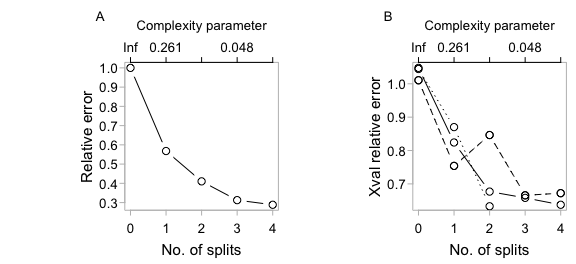
\includegraphics[width=0.9\textwidth,height=\textheight]{figs/g8_6-1.png}
\end{center}

\subsection{Section 8.3: The practicalities of tree construction -- two
examples}\label{section-8.3-the-practicalities-of-tree-construction-two-examples}

\subsubsection{Subsection 8.3.1: Data for female heart attack
patients}\label{subsection-8.3.1-data-for-female-heart-attack-patients}

\begin{Shaded}
\begin{Highlighting}[]
\NormalTok{mifem }\OtherTok{\textless{}{-}}\NormalTok{ DAAG}\SpecialCharTok{::}\NormalTok{mifem}
\FunctionTok{summary}\NormalTok{(mifem)     }\CommentTok{\# data frame mifem (DAAG)}
\end{Highlighting}
\end{Shaded}

\begin{verbatim}
 outcome         age          yronset     premi    smstat   diabetes
 live:974   Min.   :35.0   Min.   :85.0   y :311   c :390   y :248  
 dead:321   1st Qu.:57.0   1st Qu.:87.0   n :928   x :280   n :978  
            Median :63.0   Median :89.0   nk: 56   n :522   nk: 69  
            Mean   :60.9   Mean   :88.8            nk:103           
            3rd Qu.:66.0   3rd Qu.:91.0                             
            Max.   :69.0   Max.   :93.0                             
 highbp   hichol   angina   stroke   
 y :813   y :452   y :472   y : 153  
 n :406   n :655   n :724   n :1063  
 nk: 76   nk:188   nk: 99   nk:  79  
                                     
                                     
                                     
\end{verbatim}

\begin{Shaded}
\begin{Highlighting}[]
\FunctionTok{set.seed}\NormalTok{(}\DecValTok{29}\NormalTok{)      }\CommentTok{\# Make results reproducible}
\NormalTok{mifem.rpart }\OtherTok{\textless{}{-}} \FunctionTok{rpart}\NormalTok{(outcome }\SpecialCharTok{\textasciitilde{}}\NormalTok{ ., }\AttributeTok{method=}\StringTok{"class"}\NormalTok{, }\AttributeTok{data =}\NormalTok{ mifem, }\AttributeTok{cp =} \FloatTok{0.0025}\NormalTok{)}
\end{Highlighting}
\end{Shaded}

\begin{Shaded}
\begin{Highlighting}[]
\DocumentationTok{\#\# Tabular equivalent of Panel A from \textasciigrave{}plotcp(mifem.rpart)\textasciigrave{}}
\FunctionTok{printcp}\NormalTok{(mifem.rpart, }\AttributeTok{digits=}\DecValTok{3}\NormalTok{)}
\end{Highlighting}
\end{Shaded}

\begin{verbatim}

Classification tree:
rpart(formula = outcome ~ ., data = mifem, method = "class", 
    cp = 0.0025)

Variables actually used in tree construction:
[1] age      angina   diabetes hichol   premi    smstat   stroke  
[8] yronset 

Root node error: 321/1295 = 0.248

n= 1295 

       CP nsplit rel error xerror   xstd
1 0.20249      0     1.000  1.000 0.0484
2 0.00561      1     0.798  0.829 0.0453
3 0.00467     13     0.717  0.875 0.0462
4 0.00312     17     0.698  0.860 0.0459
5 0.00250     18     0.695  0.863 0.0460
\end{verbatim}

\begin{Shaded}
\begin{Highlighting}[]
\FunctionTok{cat}\NormalTok{(}\FunctionTok{c}\NormalTok{(}\StringTok{". . ."}\NormalTok{, }\FunctionTok{capture.output}\NormalTok{(}\FunctionTok{printcp}\NormalTok{(mifem.rpart, }\AttributeTok{digits=}\DecValTok{3}\NormalTok{))[}\SpecialCharTok{{-}}\NormalTok{(}\DecValTok{1}\SpecialCharTok{:}\DecValTok{9}\NormalTok{)]), }
    \AttributeTok{sep=}\StringTok{"}\SpecialCharTok{\textbackslash{}n}\StringTok{"}\NormalTok{)}
\end{Highlighting}
\end{Shaded}

\begin{verbatim}
. . .
Root node error: 321/1295 = 0.248

n= 1295 

       CP nsplit rel error xerror   xstd
1 0.20249      0     1.000  1.000 0.0484
2 0.00561      1     0.798  0.829 0.0453
3 0.00467     13     0.717  0.875 0.0462
4 0.00312     17     0.698  0.860 0.0459
5 0.00250     18     0.695  0.863 0.0460
\end{verbatim}

\begin{center}
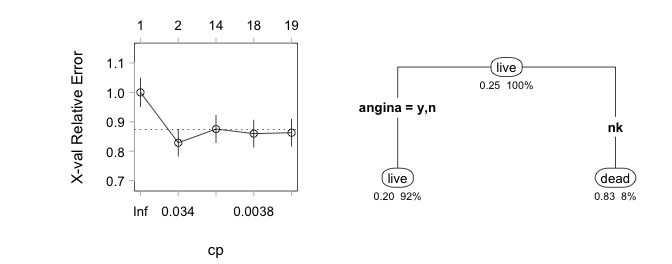
\includegraphics[width=0.75\textwidth,height=\textheight]{figs/g8_7-1.png}
\end{center}

\begin{Shaded}
\begin{Highlighting}[]
\FunctionTok{plotcp}\NormalTok{(mifem.rpart, }\AttributeTok{fg=}\StringTok{"gray"}\NormalTok{, }\AttributeTok{tcl=}\SpecialCharTok{{-}}\FloatTok{0.25}\NormalTok{)}
\NormalTok{mifemb.rpart }\OtherTok{\textless{}{-}} \FunctionTok{prune}\NormalTok{(mifem.rpart, }\AttributeTok{cp=}\FloatTok{0.01}\NormalTok{)  }\DocumentationTok{\#\# Prune tree back to 2 leaves}
\NormalTok{rpart.plot}\SpecialCharTok{::}\FunctionTok{rpart.plot}\NormalTok{(mifemb.rpart, }\AttributeTok{under=}\ConstantTok{TRUE}\NormalTok{, }\AttributeTok{type=}\DecValTok{4}\NormalTok{,}
                       \AttributeTok{box.palette=}\DecValTok{0}\NormalTok{, }\AttributeTok{tweak=}\FloatTok{1.0}\NormalTok{)}
\end{Highlighting}
\end{Shaded}

\subsubsection{Subsection 8.3.2: The one-standard-deviation
rule}\label{subsection-8.3.2-the-one-standard-deviation-rule}

\subsubsection{Subsection 8.3.3: Printed Information on Each
Split}\label{subsection-8.3.3-printed-information-on-each-split}

\begin{Shaded}
\begin{Highlighting}[]
\FunctionTok{print}\NormalTok{(mifemb.rpart)}
\end{Highlighting}
\end{Shaded}

\begin{verbatim}
n= 1295 

node), split, n, loss, yval, (yprob)
      * denotes terminal node

1) root 1295 321 live (0.7521 0.2479)  
  2) angina=y,n 1196 239 live (0.8002 0.1998) *
  3) angina=nk 99  17 dead (0.1717 0.8283) *
\end{verbatim}

\begin{Shaded}
\begin{Highlighting}[]
\FunctionTok{set.seed}\NormalTok{(}\DecValTok{59}\NormalTok{)}
\NormalTok{spam7a.rpart }\OtherTok{\textless{}{-}} \FunctionTok{rpart}\NormalTok{(}\AttributeTok{formula =}\NormalTok{ yesno }\SpecialCharTok{\textasciitilde{}}\NormalTok{ crl.tot }\SpecialCharTok{+}\NormalTok{ dollar }\SpecialCharTok{+}\NormalTok{ bang }\SpecialCharTok{+}
\NormalTok{                      money }\SpecialCharTok{+}\NormalTok{ n000 }\SpecialCharTok{+}\NormalTok{ make, }\AttributeTok{method=}\StringTok{"class"}\NormalTok{, }\AttributeTok{cp =} \FloatTok{0.002}\NormalTok{,}
                      \AttributeTok{model=}\ConstantTok{TRUE}\NormalTok{, }\AttributeTok{data =}\NormalTok{ DAAG}\SpecialCharTok{::}\NormalTok{spam7)}
\end{Highlighting}
\end{Shaded}

\begin{Shaded}
\begin{Highlighting}[]
\FunctionTok{printcp}\NormalTok{(spam7a.rpart, }\AttributeTok{digits=}\DecValTok{3}\NormalTok{)}
\end{Highlighting}
\end{Shaded}

\begin{verbatim}

Classification tree:
rpart(formula = yesno ~ crl.tot + dollar + bang + money + n000 + 
    make, data = DAAG::spam7, method = "class", model = TRUE, 
    cp = 0.002)

Variables actually used in tree construction:
[1] bang    crl.tot dollar  money   n000   

Root node error: 1813/4601 = 0.394

n= 4601 

        CP nsplit rel error xerror   xstd
1  0.47656      0     1.000  1.000 0.0183
2  0.07557      1     0.523  0.550 0.0154
3  0.01158      3     0.372  0.390 0.0135
4  0.01048      4     0.361  0.386 0.0134
5  0.00634      5     0.350  0.374 0.0133
6  0.00552     10     0.317  0.360 0.0130
7  0.00441     11     0.311  0.357 0.0130
8  0.00386     12     0.307  0.352 0.0129
9  0.00276     16     0.291  0.339 0.0127
10 0.00221     17     0.288  0.339 0.0127
11 0.00200     18     0.286  0.336 0.0127
\end{verbatim}

\begin{Shaded}
\begin{Highlighting}[]
\NormalTok{cpdf }\OtherTok{\textless{}{-}} \FunctionTok{signif}\NormalTok{(}\FunctionTok{as.data.frame}\NormalTok{(spam7a.rpart}\SpecialCharTok{$}\NormalTok{cptable),}\DecValTok{3}\NormalTok{)}
\NormalTok{minRow }\OtherTok{\textless{}{-}} \FunctionTok{which.min}\NormalTok{(cpdf[,}\StringTok{"xerror"}\NormalTok{])}
\NormalTok{upr }\OtherTok{\textless{}{-}} \FunctionTok{sum}\NormalTok{(cpdf[minRow, }\FunctionTok{c}\NormalTok{(}\StringTok{"xerror"}\NormalTok{,}\StringTok{"xstd"}\NormalTok{)])}
\NormalTok{takeRow }\OtherTok{\textless{}{-}} \FunctionTok{min}\NormalTok{((}\DecValTok{1}\SpecialCharTok{:}\NormalTok{minRow)[cpdf[}\DecValTok{1}\SpecialCharTok{:}\NormalTok{minRow,}\StringTok{"xerror"}\NormalTok{]}\SpecialCharTok{\textless{}}\NormalTok{upr])}
\NormalTok{newNsplit }\OtherTok{\textless{}{-}}\NormalTok{ cpdf[takeRow, }\StringTok{\textquotesingle{}nsplit\textquotesingle{}}\NormalTok{]}
\NormalTok{cpval }\OtherTok{\textless{}{-}} \FunctionTok{mean}\NormalTok{(cpdf[}\FunctionTok{c}\NormalTok{(takeRow}\DecValTok{{-}1}\NormalTok{,takeRow),}\StringTok{"CP"}\NormalTok{])}
\end{Highlighting}
\end{Shaded}

\begin{center}
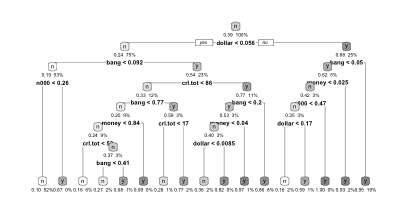
\includegraphics[width=1\textwidth,height=\textheight]{figs/g8_8-1.png}
\end{center}

\begin{Shaded}
\begin{Highlighting}[]
\NormalTok{spam7b.rpart }\OtherTok{\textless{}{-}} \FunctionTok{prune}\NormalTok{(spam7a.rpart, }\AttributeTok{cp=}\NormalTok{cpval)}
\NormalTok{rpart.plot}\SpecialCharTok{::}\FunctionTok{rpart.plot}\NormalTok{(spam7b.rpart, }\AttributeTok{under=}\ConstantTok{TRUE}\NormalTok{, }\AttributeTok{box.palette=}\StringTok{"Grays"}\NormalTok{, }\AttributeTok{tweak=}\FloatTok{1.65}\NormalTok{)}
\end{Highlighting}
\end{Shaded}

\paragraph{How does the one standard error rule affect accuracy of
estimates?}\label{how-does-the-one-standard-error-rule-affect-accuracy-of-estimates}

\begin{Shaded}
\begin{Highlighting}[]
\FunctionTok{requireNamespace}\NormalTok{(}\StringTok{\textquotesingle{}randomForest\textquotesingle{}}\NormalTok{, }\AttributeTok{quietly=}\ConstantTok{TRUE}\NormalTok{)}
\NormalTok{DAAG}\SpecialCharTok{::}\FunctionTok{compareTreecalcs}\NormalTok{(}\AttributeTok{data=}\NormalTok{DAAG}\SpecialCharTok{::}\NormalTok{spam7, }\AttributeTok{fun=}\StringTok{"rpart"}\NormalTok{)}
\end{Highlighting}
\end{Shaded}

\begin{verbatim}
 rpSEcvI    rpcvI rpSEtest   rptest  nSErule   nREmin 
  0.1396   0.1387   0.1269   0.1217   7.0000   8.0000 
\end{verbatim}

\begin{Shaded}
\begin{Highlighting}[]
\NormalTok{acctree.mat }\OtherTok{\textless{}{-}} \FunctionTok{matrix}\NormalTok{(}\DecValTok{0}\NormalTok{, }\AttributeTok{nrow=}\DecValTok{100}\NormalTok{, }\AttributeTok{ncol=}\DecValTok{6}\NormalTok{)}
\NormalTok{spam7 }\OtherTok{\textless{}{-}}\NormalTok{ DAAG}\SpecialCharTok{::}\NormalTok{spam7}
\ControlFlowTok{for}\NormalTok{(i }\ControlFlowTok{in} \DecValTok{1}\SpecialCharTok{:}\DecValTok{100}\NormalTok{)}
\NormalTok{acctree.mat[i,] }\OtherTok{\textless{}{-}}\NormalTok{ DAAG}\SpecialCharTok{::}\FunctionTok{compareTreecalcs}\NormalTok{(}\AttributeTok{data=}\NormalTok{spam7, }\AttributeTok{fun=}\StringTok{"rpart"}\NormalTok{)}
\end{Highlighting}
\end{Shaded}

\paragraph{How is the standard error
calculated?}\label{how-is-the-standard-error-calculated}

\paragraph{When are tree-based methods
appropriate?}\label{when-are-tree-based-methods-appropriate-1}

\subsection{Section 8.4: From one tree to a forest -- a more global
optimality}\label{section-8.4-from-one-tree-to-a-forest-a-more-global-optimality}

\begin{Shaded}
\begin{Highlighting}[]
\FunctionTok{suppressPackageStartupMessages}\NormalTok{(}\FunctionTok{library}\NormalTok{(randomForest))}
\NormalTok{spam7.rf }\OtherTok{\textless{}{-}} \FunctionTok{randomForest}\NormalTok{(yesno }\SpecialCharTok{\textasciitilde{}}\NormalTok{ ., }\AttributeTok{data=}\NormalTok{spam7, }\AttributeTok{importance=}\ConstantTok{TRUE}\NormalTok{)}
\NormalTok{spam7.rf}
\end{Highlighting}
\end{Shaded}

\begin{verbatim}

Call:
 randomForest(formula = yesno ~ ., data = spam7, importance = TRUE) 
               Type of random forest: classification
                     Number of trees: 500
No. of variables tried at each split: 2

        OOB estimate of  error rate: 11.56%
Confusion matrix:
     n    y class.error
n 2651  137     0.04914
y  395 1418     0.21787
\end{verbatim}

\begin{Shaded}
\begin{Highlighting}[]
\NormalTok{z }\OtherTok{\textless{}{-}} \FunctionTok{tuneRF}\NormalTok{(}\AttributeTok{x=}\NormalTok{spam7[, }\SpecialCharTok{{-}}\DecValTok{7}\NormalTok{], }\AttributeTok{y=}\NormalTok{spam7}\SpecialCharTok{$}\NormalTok{yesno, }\AttributeTok{plot=}\ConstantTok{FALSE}\NormalTok{)}
\end{Highlighting}
\end{Shaded}

\begin{verbatim}
mtry = 2  OOB error = 11.8% 
Searching left ...
mtry = 1    OOB error = 12.67% 
-0.07366 0.05 
Searching right ...
mtry = 4    OOB error = 11.76% 
0.003683 0.05 
\end{verbatim}

\begin{Shaded}
\begin{Highlighting}[]
\NormalTok{zdash }\OtherTok{\textless{}{-}} \FunctionTok{t}\NormalTok{(z[,}\DecValTok{2}\NormalTok{,}\AttributeTok{drop=}\NormalTok{F])}
\FunctionTok{colnames}\NormalTok{(zdash) }\OtherTok{\textless{}{-}} \FunctionTok{paste0}\NormalTok{(}\FunctionTok{c}\NormalTok{(}\StringTok{"mtry="}\NormalTok{,}\FunctionTok{rep}\NormalTok{(}\StringTok{""}\NormalTok{,}\DecValTok{2}\NormalTok{)), z[,}\DecValTok{1}\NormalTok{])}
\FunctionTok{round}\NormalTok{(zdash,}\DecValTok{3}\NormalTok{)}
\end{Highlighting}
\end{Shaded}

\begin{verbatim}
         mtry=1     2     4
OOBError  0.127 0.118 0.118
\end{verbatim}

\begin{Shaded}
\begin{Highlighting}[]
\FunctionTok{importance}\NormalTok{(spam7.rf)}
\end{Highlighting}
\end{Shaded}

\begin{verbatim}
            n      y MeanDecreaseAccuracy MeanDecreaseGini
crl.tot 46.73  54.19                70.57           248.10
dollar  56.21  55.35                76.13           431.75
bang    91.66 100.46               115.95           588.53
money   33.09  51.87                53.49           206.51
n000    58.25  15.74                62.29           115.46
make    13.67  21.76                26.72            41.13
\end{verbatim}

\subsubsection{Subsection 8.4.1: Prior
probabilities}\label{subsection-8.4.1-prior-probabilities}

\begin{Shaded}
\begin{Highlighting}[]
\NormalTok{Pima.tr }\OtherTok{\textless{}{-}}\NormalTok{ MASS}\SpecialCharTok{::}\NormalTok{Pima.tr}
\FunctionTok{table}\NormalTok{(Pima.tr}\SpecialCharTok{$}\NormalTok{type)}
\end{Highlighting}
\end{Shaded}

\begin{verbatim}

 No Yes 
132  68 
\end{verbatim}

\begin{Shaded}
\begin{Highlighting}[]
\FunctionTok{set.seed}\NormalTok{(}\DecValTok{41}\NormalTok{)     }\CommentTok{\# This seed should reproduce the result given here}
\NormalTok{Pima.rf }\OtherTok{\textless{}{-}} \FunctionTok{randomForest}\NormalTok{(type }\SpecialCharTok{\textasciitilde{}}\NormalTok{ ., }\AttributeTok{data=}\NormalTok{Pima.tr)}
\DocumentationTok{\#\# The above is equivalent to:}
\DocumentationTok{\#\# Pima.rf \textless{}{-} randomForest(type \textasciitilde{} ., data=Pima.tr, sampsize=200)}
\FunctionTok{round}\NormalTok{(Pima.rf}\SpecialCharTok{$}\NormalTok{confusion,}\DecValTok{3}\NormalTok{)}
\end{Highlighting}
\end{Shaded}

\begin{verbatim}
     No Yes class.error
No  110  22       0.167
Yes  32  36       0.471
\end{verbatim}

\begin{Shaded}
\begin{Highlighting}[]
\NormalTok{tab }\OtherTok{\textless{}{-}} \FunctionTok{prop.table}\NormalTok{(}\FunctionTok{table}\NormalTok{(Pima.tr}\SpecialCharTok{$}\NormalTok{type))}
\end{Highlighting}
\end{Shaded}

\begin{Shaded}
\begin{Highlighting}[]
\NormalTok{Pima.rf }\OtherTok{\textless{}{-}} \FunctionTok{randomForest}\NormalTok{(type }\SpecialCharTok{\textasciitilde{}}\NormalTok{ ., }\AttributeTok{data=}\NormalTok{Pima.tr, }\AttributeTok{sampsize=}\FunctionTok{c}\NormalTok{(}\DecValTok{68}\NormalTok{,}\DecValTok{68}\NormalTok{))}
\end{Highlighting}
\end{Shaded}

\begin{Shaded}
\begin{Highlighting}[]
\NormalTok{Pima.rf }\OtherTok{\textless{}{-}} \FunctionTok{randomForest}\NormalTok{(type }\SpecialCharTok{\textasciitilde{}}\NormalTok{ ., }\AttributeTok{data=}\NormalTok{Pima.tr, }\AttributeTok{sampsize=}\FunctionTok{c}\NormalTok{(}\DecValTok{132}\NormalTok{,}\DecValTok{68}\NormalTok{))}
\end{Highlighting}
\end{Shaded}

\subsubsection{Subsection 8.4.2: A low-dimensional representation of
observations}\label{subsection-8.4.2-a-low-dimensional-representation-of-observations}

\subsubsection{Subsection 8.4.3: Models with a complex error
structure}\label{subsection-8.4.3-models-with-a-complex-error-structure}

\subsection{Section 8.5: Additional notes -- one tree, or many
trees?}\label{section-8.5-additional-notes-one-tree-or-many-trees}

\subsubsection{Subsection 8.5.1: Differences between rpart() and
randomForest()}\label{subsection-8.5.1-differences-between-rpart-and-randomforest}

\paragraph{Error rates -- rpart() versus
randomForest()}\label{error-rates-rpart-versus-randomforest}

\begin{center}
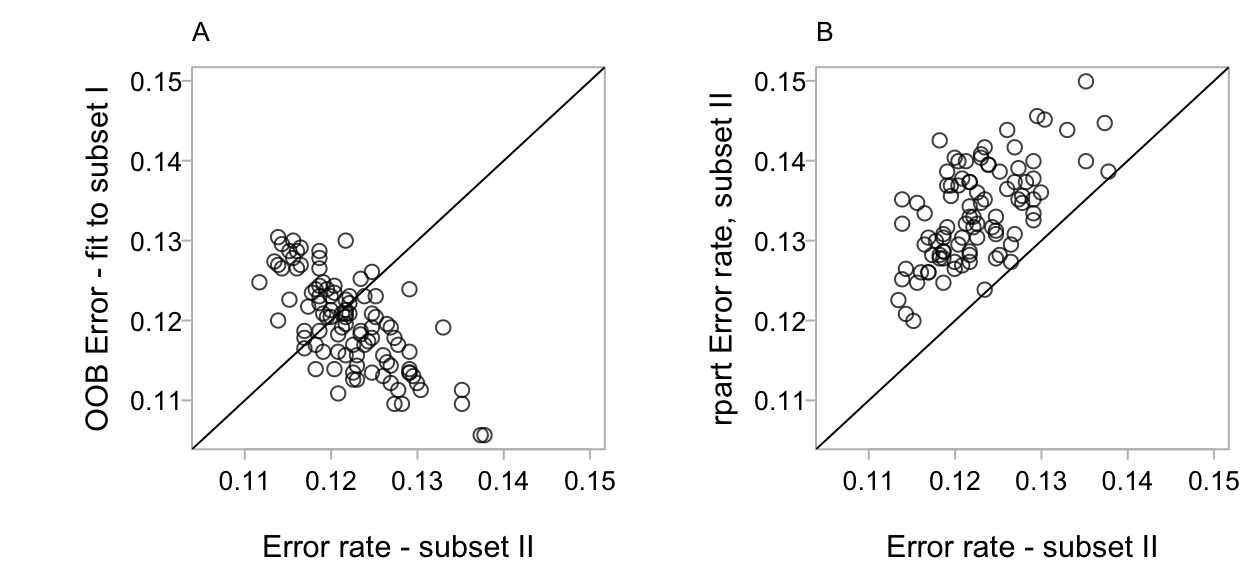
\includegraphics[width=0.8\textwidth,height=\textheight]{figs/g8_9-1.png}
\end{center}

\begin{Shaded}
\begin{Highlighting}[]
\DocumentationTok{\#\# Accuracy comparisons}
\NormalTok{acctree.mat }\OtherTok{\textless{}{-}} \FunctionTok{matrix}\NormalTok{(}\DecValTok{0}\NormalTok{, }\AttributeTok{nrow=}\DecValTok{100}\NormalTok{, }\AttributeTok{ncol=}\DecValTok{8}\NormalTok{)}
\FunctionTok{colnames}\NormalTok{(acctree.mat) }\OtherTok{\textless{}{-}} \FunctionTok{c}\NormalTok{(}\StringTok{"rpSEcvI"}\NormalTok{, }\StringTok{"rpcvI"}\NormalTok{, }\StringTok{"rpSEtest"}\NormalTok{, }\StringTok{"rptest"}\NormalTok{,}
                          \StringTok{"n.SErule"}\NormalTok{, }\StringTok{"nre.min.12"}\NormalTok{, }\StringTok{"rfOOBI"}\NormalTok{, }\StringTok{"rftest"}\NormalTok{)}
\ControlFlowTok{for}\NormalTok{(i }\ControlFlowTok{in} \DecValTok{1}\SpecialCharTok{:}\DecValTok{100}\NormalTok{)acctree.mat[i,] }\OtherTok{\textless{}{-}}\NormalTok{ DAAG}\SpecialCharTok{::}\FunctionTok{compareTreecalcs}\NormalTok{(}\AttributeTok{data=}\NormalTok{spam7, }\AttributeTok{cp=}\FloatTok{0.0004}\NormalTok{,}
                                          \AttributeTok{fun=}\FunctionTok{c}\NormalTok{(}\StringTok{"rpart"}\NormalTok{, }\StringTok{"randomForest"}\NormalTok{))}
\NormalTok{acctree.df }\OtherTok{\textless{}{-}} \FunctionTok{data.frame}\NormalTok{(acctree.mat)}
\NormalTok{lims }\OtherTok{\textless{}{-}} \FunctionTok{range}\NormalTok{(acctree.mat[, }\FunctionTok{c}\NormalTok{(}\DecValTok{4}\NormalTok{,}\DecValTok{7}\NormalTok{,}\DecValTok{8}\NormalTok{)], }\AttributeTok{na.rm=}\ConstantTok{TRUE}\NormalTok{)}
\NormalTok{cthrublack }\OtherTok{\textless{}{-}} \FunctionTok{adjustcolor}\NormalTok{(}\StringTok{"black"}\NormalTok{, }\AttributeTok{alpha.f=}\FloatTok{0.75}\NormalTok{)}
\CommentTok{\# Panel A}
\FunctionTok{plot}\NormalTok{(rfOOBI }\SpecialCharTok{\textasciitilde{}}\NormalTok{ rftest, }\AttributeTok{data=}\NormalTok{acctree.df, }\AttributeTok{xlab=}\StringTok{"Error rate {-} subset II"}\NormalTok{, }\AttributeTok{xlim=}\NormalTok{lims,}
     \AttributeTok{ylim=}\NormalTok{lims, }\AttributeTok{ylab=}\StringTok{"OOB Error {-} fit to subset I"}\NormalTok{, }\AttributeTok{col=}\NormalTok{cthrublack, }\AttributeTok{fg=}\StringTok{"gray"}\NormalTok{)}
\FunctionTok{abline}\NormalTok{(}\DecValTok{0}\NormalTok{,}\DecValTok{1}\NormalTok{)}
\FunctionTok{mtext}\NormalTok{(}\AttributeTok{side=}\DecValTok{3}\NormalTok{, }\AttributeTok{line=}\FloatTok{0.5}\NormalTok{, }\StringTok{"A"}\NormalTok{, }\AttributeTok{adj=}\DecValTok{0}\NormalTok{)}
\CommentTok{\# Panel B}
\FunctionTok{plot}\NormalTok{(rptest }\SpecialCharTok{\textasciitilde{}}\NormalTok{ rftest, }\AttributeTok{data=}\NormalTok{acctree.df, }\AttributeTok{xlab=}\StringTok{"Error rate {-} subset II"}\NormalTok{,}
     \AttributeTok{ylab=}\StringTok{"rpart Error rate, subset II"}\NormalTok{, }\AttributeTok{xlim=}\NormalTok{lims, }\AttributeTok{ylim=}\NormalTok{lims,}
     \AttributeTok{col=}\NormalTok{cthrublack, }\AttributeTok{fg=}\StringTok{"gray"}\NormalTok{)}
\FunctionTok{abline}\NormalTok{(}\DecValTok{0}\NormalTok{,}\DecValTok{1}\NormalTok{)}
\FunctionTok{mtext}\NormalTok{(}\AttributeTok{side=}\DecValTok{3}\NormalTok{, }\AttributeTok{line=}\FloatTok{0.5}\NormalTok{, }\StringTok{"B"}\NormalTok{, }\AttributeTok{adj=}\DecValTok{0}\NormalTok{)}
\end{Highlighting}
\end{Shaded}

\begin{Shaded}
\begin{Highlighting}[]
\NormalTok{acctree.mat }\OtherTok{\textless{}{-}} \FunctionTok{matrix}\NormalTok{(}\DecValTok{0}\NormalTok{, }\AttributeTok{nrow=}\DecValTok{100}\NormalTok{, }\AttributeTok{ncol=}\DecValTok{8}\NormalTok{)}
\FunctionTok{colnames}\NormalTok{(acctree.mat) }\OtherTok{\textless{}{-}} \FunctionTok{c}\NormalTok{(}\StringTok{"rpSEcvI"}\NormalTok{, }\StringTok{"rpcvI"}\NormalTok{, }\StringTok{"rpSEtest"}\NormalTok{, }\StringTok{"rptest"}\NormalTok{,}
                          \StringTok{"n.SErule"}\NormalTok{, }\StringTok{"nre.min.12"}\NormalTok{, }\StringTok{"rfcvI"}\NormalTok{, }\StringTok{"rftest"}\NormalTok{)}
\ControlFlowTok{for}\NormalTok{(i }\ControlFlowTok{in} \DecValTok{1}\SpecialCharTok{:}\DecValTok{100}\NormalTok{)acctree.mat[i,] }\OtherTok{\textless{}{-}}\NormalTok{ DAAG}\SpecialCharTok{::}\FunctionTok{compareTreecalcs}\NormalTok{(}\AttributeTok{data=}\NormalTok{spam7,}
                                          \AttributeTok{fun=}\FunctionTok{c}\NormalTok{(}\StringTok{"rpart"}\NormalTok{, }\StringTok{"randomForest"}\NormalTok{))}
\DocumentationTok{\#\# Panel A: Plot \textasciigrave{}rfOOBI\textasciigrave{} against \textasciigrave{}rftest\textasciigrave{}}
\DocumentationTok{\#\# Panel B: Plot \textasciigrave{}rptest\textasciigrave{} against \textasciigrave{}rftest\textasciigrave{}}
\end{Highlighting}
\end{Shaded}

\paragraph{Times required for
computation}\label{times-required-for-computation}

\subsubsection{Subsection 8.5.2: Tree-based methods, versus other
approaches}\label{subsection-8.5.2-tree-based-methods-versus-other-approaches}

\paragraph{Tree-based methods may usefully complement other
approaches}\label{tree-based-methods-may-usefully-complement-other-approaches}

\subsubsection{Subsection 8.5.3: Further
notes}\label{subsection-8.5.3-further-notes}

\paragraph{Pruning as variable
selection}\label{pruning-as-variable-selection}

\subsection{Section 8.6: Further reading and
extensions}\label{section-8.6-further-reading-and-extensions}

\subsection{Exercises (8.7)}\label{exercises-8.7}

8.5

\begin{Shaded}
\begin{Highlighting}[]
\FunctionTok{sapply}\NormalTok{(MASS}\SpecialCharTok{::}\NormalTok{biopsy, }\ControlFlowTok{function}\NormalTok{(x)}\FunctionTok{sum}\NormalTok{(}\FunctionTok{is.na}\NormalTok{(x)))   }\DocumentationTok{\#\# Will omit rows with NAs}
\end{Highlighting}
\end{Shaded}

\begin{verbatim}
   ID    V1    V2    V3    V4    V5    V6    V7    V8    V9 class 
    0     0     0     0     0     0    16     0     0     0     0 
\end{verbatim}

\begin{Shaded}
\begin{Highlighting}[]
\NormalTok{biops }\OtherTok{\textless{}{-}} \FunctionTok{na.omit}\NormalTok{(MASS}\SpecialCharTok{::}\NormalTok{biopsy)[,}\SpecialCharTok{{-}}\DecValTok{1}\NormalTok{]               }\DocumentationTok{\#\# Omit also column 1 (IDs)}
\DocumentationTok{\#\# Examine list element names in randomForest object}
\FunctionTok{names}\NormalTok{(}\FunctionTok{randomForest}\NormalTok{(class }\SpecialCharTok{\textasciitilde{}}\NormalTok{ ., }\AttributeTok{data=}\NormalTok{biops))}
\end{Highlighting}
\end{Shaded}

\begin{verbatim}
 [1] "call"            "type"            "predicted"      
 [4] "err.rate"        "confusion"       "votes"          
 [7] "oob.times"       "classes"         "importance"     
[10] "importanceSD"    "localImportance" "proximity"      
[13] "ntree"           "mtry"            "forest"         
[16] "y"               "test"            "inbag"          
[19] "terms"          
\end{verbatim}

8.5a

\begin{Shaded}
\begin{Highlighting}[]
\DocumentationTok{\#\# Repeated runs, note variation in OOB accuracy.}
\ControlFlowTok{for}\NormalTok{(i }\ControlFlowTok{in} \DecValTok{1}\SpecialCharTok{:}\DecValTok{10}\NormalTok{) \{}
\NormalTok{  biops.rf }\OtherTok{\textless{}{-}} \FunctionTok{randomForest}\NormalTok{(class }\SpecialCharTok{\textasciitilde{}}\NormalTok{ ., }\AttributeTok{data=}\NormalTok{biops)  }
\NormalTok{  OOBerr }\OtherTok{\textless{}{-}} \FunctionTok{mean}\NormalTok{(biops.rf}\SpecialCharTok{$}\NormalTok{err.rate[,}\StringTok{"OOB"}\NormalTok{])}
  \FunctionTok{print}\NormalTok{(}\FunctionTok{paste}\NormalTok{(i, }\StringTok{": "}\NormalTok{, }\FunctionTok{round}\NormalTok{(OOBerr, }\DecValTok{4}\NormalTok{), }\AttributeTok{sep=}\StringTok{""}\NormalTok{))}
  \FunctionTok{print}\NormalTok{(}\FunctionTok{round}\NormalTok{(biops.rf}\SpecialCharTok{$}\NormalTok{confusion,}\DecValTok{4}\NormalTok{))}
\NormalTok{\}}
\end{Highlighting}
\end{Shaded}

\begin{verbatim}
[1] "1: 0.0288"
          benign malignant class.error
benign       432        12      0.0270
malignant      7       232      0.0293
[1] "2: 0.0344"
          benign malignant class.error
benign       431        13      0.0293
malignant      9       230      0.0377
[1] "3: 0.0308"
          benign malignant class.error
benign       433        11      0.0248
malignant      9       230      0.0377
[1] "4: 0.0307"
          benign malignant class.error
benign       431        13      0.0293
malignant      6       233      0.0251
[1] "5: 0.0311"
          benign malignant class.error
benign       433        11      0.0248
malignant      8       231      0.0335
[1] "6: 0.0301"
          benign malignant class.error
benign       431        13      0.0293
malignant      6       233      0.0251
[1] "7: 0.0312"
          benign malignant class.error
benign       433        11      0.0248
malignant      7       232      0.0293
[1] "8: 0.0301"
          benign malignant class.error
benign       433        11      0.0248
malignant      8       231      0.0335
[1] "9: 0.0285"
          benign malignant class.error
benign       433        11      0.0248
malignant      6       233      0.0251
[1] "10: 0.0301"
          benign malignant class.error
benign       432        12      0.0270
malignant      7       232      0.0293
\end{verbatim}

8.5b

\begin{Shaded}
\begin{Highlighting}[]
\DocumentationTok{\#\# Repeated train/test splits: OOB accuracy vs test set accuracy.}
\ControlFlowTok{for}\NormalTok{(i }\ControlFlowTok{in} \DecValTok{1}\SpecialCharTok{:}\DecValTok{10}\NormalTok{)\{}
\NormalTok{  trRows }\OtherTok{\textless{}{-}} \FunctionTok{sample}\NormalTok{(}\DecValTok{1}\SpecialCharTok{:}\FunctionTok{dim}\NormalTok{(biops)[}\DecValTok{1}\NormalTok{], }\AttributeTok{size=}\FunctionTok{round}\NormalTok{(}\FunctionTok{dim}\NormalTok{(biops)[}\DecValTok{1}\NormalTok{]}\SpecialCharTok{/}\DecValTok{2}\NormalTok{))}
\NormalTok{  biops.rf }\OtherTok{\textless{}{-}} \FunctionTok{randomForest}\NormalTok{(class }\SpecialCharTok{\textasciitilde{}}\NormalTok{ ., }\AttributeTok{data=}\NormalTok{biops[trRows, ],}
    \AttributeTok{xtest=}\NormalTok{biops[}\SpecialCharTok{{-}}\NormalTok{trRows,}\SpecialCharTok{{-}}\DecValTok{10}\NormalTok{], }\AttributeTok{ytest=}\NormalTok{biops[}\SpecialCharTok{{-}}\NormalTok{trRows,}\DecValTok{10}\NormalTok{])}
\NormalTok{  oobErr }\OtherTok{\textless{}{-}} \FunctionTok{mean}\NormalTok{(biops.rf}\SpecialCharTok{$}\NormalTok{err.rate[,}\StringTok{"OOB"}\NormalTok{])}
\NormalTok{  testErr }\OtherTok{\textless{}{-}} \FunctionTok{mean}\NormalTok{(biops.rf}\SpecialCharTok{$}\NormalTok{test}\SpecialCharTok{$}\NormalTok{err.rate[,}\StringTok{"Test"}\NormalTok{])}
\FunctionTok{print}\NormalTok{(}\FunctionTok{round}\NormalTok{(}\FunctionTok{c}\NormalTok{(oobErr,testErr),}\DecValTok{4}\NormalTok{))}
\NormalTok{\}}
\end{Highlighting}
\end{Shaded}

\begin{verbatim}
[1] 0.0282 0.0340
[1] 0.0366 0.0327
[1] 0.0360 0.0226
[1] 0.0330 0.0311
[1] 0.0360 0.0384
[1] 0.0357 0.0353
[1] 0.0248 0.0399
[1] 0.0442 0.0270
[1] 0.0407 0.0268
[1] 0.0347 0.0242
\end{verbatim}

8.5c

\begin{Shaded}
\begin{Highlighting}[]
\FunctionTok{randomForest}\NormalTok{(class }\SpecialCharTok{\textasciitilde{}}\NormalTok{ ., }\AttributeTok{data=}\NormalTok{biops, }\AttributeTok{xtest=}\NormalTok{biops[,}\SpecialCharTok{{-}}\DecValTok{10}\NormalTok{], }\AttributeTok{ytest=}\NormalTok{biops[,}\DecValTok{10}\NormalTok{])}
\end{Highlighting}
\end{Shaded}

\begin{verbatim}

Call:
 randomForest(formula = class ~ ., data = biops, xtest = biops[,      -10], ytest = biops[, 10]) 
               Type of random forest: classification
                     Number of trees: 500
No. of variables tried at each split: 3

        OOB estimate of  error rate: 2.93%
Confusion matrix:
          benign malignant class.error
benign       433        11     0.02477
malignant      9       230     0.03766
                Test set error rate: 0%
Confusion matrix:
          benign malignant class.error
benign       444         0           0
malignant      0       239           0
\end{verbatim}

8.7

\begin{Shaded}
\begin{Highlighting}[]
\DocumentationTok{\#\# Run model on total data}
\FunctionTok{randomForest}\NormalTok{(}\FunctionTok{as.factor}\NormalTok{(type) }\SpecialCharTok{\textasciitilde{}}\NormalTok{ ., }\AttributeTok{data=}\NormalTok{Pima.tr)}
\end{Highlighting}
\end{Shaded}

\begin{verbatim}

Call:
 randomForest(formula = as.factor(type) ~ ., data = Pima.tr) 
               Type of random forest: classification
                     Number of trees: 500
No. of variables tried at each split: 2

        OOB estimate of  error rate: 28%
Confusion matrix:
     No Yes class.error
No  109  23      0.1742
Yes  33  35      0.4853
\end{verbatim}

\begin{Shaded}
\begin{Highlighting}[]
\NormalTok{rowsamp }\OtherTok{\textless{}{-}} \FunctionTok{sample}\NormalTok{(}\FunctionTok{dim}\NormalTok{(Pima.tr)[}\DecValTok{1}\NormalTok{], }\AttributeTok{replace=}\ConstantTok{TRUE}\NormalTok{)}
\FunctionTok{randomForest}\NormalTok{(}\FunctionTok{as.factor}\NormalTok{(type) }\SpecialCharTok{\textasciitilde{}}\NormalTok{ ., }\AttributeTok{data=}\NormalTok{Pima.tr[rowsamp, ])}
\end{Highlighting}
\end{Shaded}

\begin{verbatim}

Call:
 randomForest(formula = as.factor(type) ~ ., data = Pima.tr[rowsamp,      ]) 
               Type of random forest: classification
                     Number of trees: 500
No. of variables tried at each split: 2

        OOB estimate of  error rate: 8.5%
Confusion matrix:
     No Yes class.error
No  129   3     0.02273
Yes  14  54     0.20588
\end{verbatim}

8.8a

\begin{Shaded}
\begin{Highlighting}[]
\NormalTok{d500 }\OtherTok{\textless{}{-}}\NormalTok{ ggplot2}\SpecialCharTok{::}\NormalTok{diamonds[}\FunctionTok{sample}\NormalTok{(}\DecValTok{1}\SpecialCharTok{:}\FunctionTok{nrow}\NormalTok{(ggplot2}\SpecialCharTok{::}\NormalTok{diamonds), }\DecValTok{500}\NormalTok{),]}
\FunctionTok{unlist}\NormalTok{(}\FunctionTok{sapply}\NormalTok{(d500, class))  }\CommentTok{\# Check the class of the 10 columns}
\end{Highlighting}
\end{Shaded}

\begin{verbatim}
    carat      cut1      cut2    color1    color2  clarity1  clarity2 
"numeric" "ordered"  "factor" "ordered"  "factor" "ordered"  "factor" 
    depth     table     price         x         y         z 
"numeric" "numeric" "integer" "numeric" "numeric" "numeric" 
\end{verbatim}

\begin{Shaded}
\begin{Highlighting}[]
\NormalTok{car}\SpecialCharTok{::}\FunctionTok{spm}\NormalTok{(d500)       }\CommentTok{\# If screen space is limited do two plots, thus:}
  \CommentTok{\# 1) variables 1 to 5 and 7 (\textasciigrave{}price\textasciigrave{}); 2) variables 6 to 10}
\FunctionTok{plot}\NormalTok{(}\FunctionTok{density}\NormalTok{(d500[, }\StringTok{"price"}\NormalTok{, }\AttributeTok{drop =}\NormalTok{ T]))         }\CommentTok{\# Distribution is highly skew}
\NormalTok{MASS}\SpecialCharTok{::}\FunctionTok{boxcox}\NormalTok{(price}\SpecialCharTok{\textasciitilde{}}\NormalTok{., }\AttributeTok{data=}\NormalTok{ggplot2}\SpecialCharTok{::}\NormalTok{diamonds)  }\CommentTok{\# Suggests log transformation}
\end{Highlighting}
\end{Shaded}

\begin{center}
\includegraphics[width=0.8\textwidth,height=\textheight]{figs/gH7f-1.png}
\end{center}

\begin{center}
\includegraphics[width=0.8\textwidth,height=\textheight]{figs/gH7f-2.png}
\end{center}

\begin{center}
\includegraphics[width=0.8\textwidth,height=\textheight]{figs/gH7f-3.png}
\end{center}

8.8b

\begin{Shaded}
\begin{Highlighting}[]
\NormalTok{diamonds }\OtherTok{\textless{}{-}}\NormalTok{ ggplot2}\SpecialCharTok{::}\NormalTok{diamonds; Y }\OtherTok{\textless{}{-}}\NormalTok{ diamonds[,}\StringTok{"price"}\NormalTok{, drop}\OtherTok{=}\NormalTok{T]}
\FunctionTok{library}\NormalTok{(rpart)}
\NormalTok{d7.rpart }\OtherTok{\textless{}{-}} \FunctionTok{rpart}\NormalTok{(}\FunctionTok{log}\NormalTok{(Y) }\SpecialCharTok{\textasciitilde{}}\NormalTok{ ., }\AttributeTok{data=}\NormalTok{diamonds[,}\SpecialCharTok{{-}}\DecValTok{7}\NormalTok{], }\AttributeTok{cp=}\FloatTok{5e{-}7}\NormalTok{) }\CommentTok{\# Complex tree}
\NormalTok{d.rpart }\OtherTok{\textless{}{-}} \FunctionTok{prune}\NormalTok{(d7.rpart, }\AttributeTok{cp=}\FloatTok{0.0025}\NormalTok{)            }
\FunctionTok{printcp}\NormalTok{(d.rpart)   }\CommentTok{\# Relative to \textasciigrave{}d7.rpart\textasciigrave{}, simpler and less accurate}
\end{Highlighting}
\end{Shaded}

\begin{verbatim}

Regression tree:
rpart(formula = log(Y) ~ ., data = diamonds[, -7], cp = 0.0000005)

Variables actually used in tree construction:
[1] carat   clarity color   x       y      

Root node error: 55531/53940 = 1

n= 53940 

       CP nsplit rel error xerror    xstd
1  0.7244      0     1.000  1.000 0.00409
2  0.0885      1     0.276  0.276 0.00141
3  0.0661      2     0.187  0.188 0.00104
4  0.0290      3     0.121  0.121 0.00075
5  0.0105      4     0.092  0.092 0.00059
6  0.0072      5     0.082  0.082 0.00054
7  0.0071      6     0.074  0.072 0.00049
8  0.0030      7     0.067  0.068 0.00047
9  0.0026      8     0.064  0.065 0.00046
10 0.0026      9     0.062  0.061 0.00044
11 0.0025     10     0.059  0.059 0.00044
\end{verbatim}

\begin{Shaded}
\begin{Highlighting}[]
\NormalTok{nmin }\OtherTok{\textless{}{-}} \FunctionTok{which.min}\NormalTok{(d7.rpart}\SpecialCharTok{$}\NormalTok{cptable[,}\StringTok{\textquotesingle{}xerror\textquotesingle{}}\NormalTok{])}
\NormalTok{dOpt.rpart }\OtherTok{\textless{}{-}} \FunctionTok{prune}\NormalTok{(d7.rpart, }\AttributeTok{cp=}\NormalTok{d7.rpart}\SpecialCharTok{$}\NormalTok{cptable[nmin,}\StringTok{\textquotesingle{}CP\textquotesingle{}}\NormalTok{])}
\FunctionTok{print}\NormalTok{(dOpt.rpart}\SpecialCharTok{$}\NormalTok{cptable[nmin])}
\end{Highlighting}
\end{Shaded}

\begin{verbatim}
[1] 0.0000008743
\end{verbatim}

\begin{Shaded}
\begin{Highlighting}[]
\NormalTok{(xerror12 }\OtherTok{\textless{}{-}}\NormalTok{ dOpt.rpart}\SpecialCharTok{$}\NormalTok{cptable[}\FunctionTok{c}\NormalTok{(}\FunctionTok{nrow}\NormalTok{(d.rpart}\SpecialCharTok{$}\NormalTok{cptable),nmin), }\StringTok{"xerror"}\NormalTok{])}
\end{Highlighting}
\end{Shaded}

\begin{verbatim}
     11    1931 
0.05934 0.01074 
\end{verbatim}

\begin{Shaded}
\begin{Highlighting}[]
 \DocumentationTok{\#\# Subtract from 1.0 to obtain R{-}squared statistics}
\end{Highlighting}
\end{Shaded}

\begin{Shaded}
\begin{Highlighting}[]
\FunctionTok{rbind}\NormalTok{(}\StringTok{"d.rpart"}\OtherTok{=}\NormalTok{d.rpart[[}\StringTok{\textquotesingle{}variable.importance\textquotesingle{}}\NormalTok{]],}
      \StringTok{"dOpt.rpart"}\OtherTok{=}\NormalTok{dOpt.rpart[[}\StringTok{\textquotesingle{}variable.importance\textquotesingle{}}\NormalTok{]]) }\SpecialCharTok{|\textgreater{}}
\NormalTok{  (\textbackslash{}(x)}\DecValTok{100}\SpecialCharTok{*}\FunctionTok{apply}\NormalTok{(x,}\DecValTok{1}\NormalTok{,}\ControlFlowTok{function}\NormalTok{(x)x}\SpecialCharTok{/}\FunctionTok{sum}\NormalTok{(x)))() }\SpecialCharTok{|\textgreater{}} \FunctionTok{round}\NormalTok{(}\DecValTok{1}\NormalTok{) }\SpecialCharTok{|\textgreater{}} \FunctionTok{t}\NormalTok{()}
\end{Highlighting}
\end{Shaded}

\begin{verbatim}
              y    x carat    z clarity table color depth cut
d.rpart    23.8 23.1  22.9 22.4     4.8   2.8   0.2   0.1 0.1
dOpt.rpart 23.5 22.9  22.7 22.2     5.2   2.7   0.5   0.2 0.1
\end{verbatim}

8.9

\begin{Shaded}
\begin{Highlighting}[]
\NormalTok{Y }\OtherTok{\textless{}{-}}\NormalTok{ ggplot2}\SpecialCharTok{::}\NormalTok{diamonds[,}\StringTok{"price"}\NormalTok{, drop}\OtherTok{=}\NormalTok{T]}
\NormalTok{samp5K }\OtherTok{\textless{}{-}} \FunctionTok{sample}\NormalTok{(}\DecValTok{1}\SpecialCharTok{:}\FunctionTok{nrow}\NormalTok{(diamonds), }\AttributeTok{size=}\DecValTok{5000}\NormalTok{)}
\NormalTok{(diamond5K.rf }\OtherTok{\textless{}{-}} \FunctionTok{randomForest}\NormalTok{(}\AttributeTok{x=}\NormalTok{diamonds[samp5K,}\SpecialCharTok{{-}}\DecValTok{7}\NormalTok{], }\AttributeTok{y=}\FunctionTok{log}\NormalTok{(Y[samp5K]),}
                   \AttributeTok{xtest=}\NormalTok{diamonds[}\SpecialCharTok{{-}}\NormalTok{samp5K,}\SpecialCharTok{{-}}\DecValTok{7}\NormalTok{], }\AttributeTok{ytest=}\FunctionTok{log}\NormalTok{(Y[}\SpecialCharTok{{-}}\NormalTok{samp5K])))}
\end{Highlighting}
\end{Shaded}

\begin{verbatim}

Call:
 randomForest(x = diamonds[samp5K, -7], y = log(Y[samp5K]), xtest = diamonds[-samp5K,      -7], ytest = log(Y[-samp5K])) 
               Type of random forest: regression
                     Number of trees: 500
No. of variables tried at each split: 3

          Mean of squared residuals: 0.01434
                    % Var explained: 98.59
                       Test set MSE: 0.01
                    % Var explained: 98.65
\end{verbatim}

\begin{Shaded}
\begin{Highlighting}[]
\DocumentationTok{\#\# Omit arguments \textasciigrave{}xtest\textasciigrave{} and \textasciigrave{}ytest\textasciigrave{} if calculations take too long}
\end{Highlighting}
\end{Shaded}

\begin{Shaded}
\begin{Highlighting}[]
\FunctionTok{sort}\NormalTok{(}\FunctionTok{importance}\NormalTok{(diamond5K.rf)[,}\DecValTok{1}\NormalTok{], }\AttributeTok{decreasing=}\NormalTok{T) }\SpecialCharTok{|\textgreater{}} 
\NormalTok{  (\textbackslash{}(x)}\DecValTok{100}\SpecialCharTok{*}\NormalTok{x}\SpecialCharTok{/}\FunctionTok{sum}\NormalTok{(x))() }\SpecialCharTok{|\textgreater{}} \FunctionTok{round}\NormalTok{(}\DecValTok{1}\NormalTok{) }\SpecialCharTok{|\textgreater{}} \FunctionTok{t}\NormalTok{()}
\end{Highlighting}
\end{Shaded}

\begin{verbatim}
        y carat  x    z clarity color depth table cut
[1,] 33.5  23.6 21 17.2     2.6   1.2   0.4   0.3 0.2
\end{verbatim}

8.9a

\begin{Shaded}
\begin{Highlighting}[]
\NormalTok{(diamond5KU.rf }\OtherTok{\textless{}{-}} \FunctionTok{randomForest}\NormalTok{(}\AttributeTok{x=}\NormalTok{diamonds[samp5K,}\SpecialCharTok{{-}}\DecValTok{7}\NormalTok{], }\AttributeTok{y=}\NormalTok{Y[samp5K],}
                   \AttributeTok{xtest=}\NormalTok{diamonds[}\SpecialCharTok{{-}}\NormalTok{samp5K,}\SpecialCharTok{{-}}\DecValTok{7}\NormalTok{], }\AttributeTok{ytest=}\NormalTok{Y[}\SpecialCharTok{{-}}\NormalTok{samp5K]))}
\end{Highlighting}
\end{Shaded}

\begin{verbatim}

Call:
 randomForest(x = diamonds[samp5K, -7], y = Y[samp5K], xtest = diamonds[-samp5K,      -7], ytest = Y[-samp5K]) 
               Type of random forest: regression
                     Number of trees: 500
No. of variables tried at each split: 3

          Mean of squared residuals: 450742
                    % Var explained: 97.11
                       Test set MSE: 493916
                    % Var explained: 96.9
\end{verbatim}

\begin{Shaded}
\begin{Highlighting}[]
\ControlFlowTok{if}\NormalTok{(}\FunctionTok{file.exists}\NormalTok{(}\StringTok{"/Users/johnm1/pkgs/PGRcode/inst/doc/"}\NormalTok{))\{}
\NormalTok{code }\OtherTok{\textless{}{-}}\NormalTok{ knitr}\SpecialCharTok{::}\NormalTok{knit\_code}\SpecialCharTok{$}\FunctionTok{get}\NormalTok{()}
\NormalTok{txt }\OtherTok{\textless{}{-}} \FunctionTok{paste0}\NormalTok{(}\StringTok{"}\SpecialCharTok{\textbackslash{}n}\StringTok{\#\# "}\NormalTok{, }\FunctionTok{names}\NormalTok{(code),}\StringTok{"}\SpecialCharTok{\textbackslash{}n}\StringTok{"}\NormalTok{, }\FunctionTok{sapply}\NormalTok{(code, paste, }\AttributeTok{collapse=}\StringTok{\textquotesingle{}}\SpecialCharTok{\textbackslash{}n}\StringTok{\textquotesingle{}}\NormalTok{))}
\FunctionTok{writeLines}\NormalTok{(txt, }\AttributeTok{con=}\StringTok{"/Users/johnm1/pkgs/PGRcode/inst/doc/ch8.R"}\NormalTok{)}
\NormalTok{\}}
\end{Highlighting}
\end{Shaded}

\bookmarksetup{startatroot}

\chapter{Chapter 9: Multivariate data exploration and
discrimination}\label{chapter-9-multivariate-data-exploration-and-discrimination}

\paragraph{Packages required (plus any
dependencies)}\label{packages-required-plus-any-dependencies-6}

Packages used are: DAAG MASS RColorBrewer teigen BiocManager DAAGbio
hddplot lmtest splines cobalt mice datasets car micemd oz randomForest
ggplot2 latticeExtra mvtnorm teigen limma hddplot mgcv MatchIt sandwich
gridExtra DAAGbio mlbench (exercise).

Additionally, knitr and Hmisc are required in order to process the Rmd
source file.

\begin{Shaded}
\begin{Highlighting}[]
\NormalTok{Hmisc}\SpecialCharTok{::}\FunctionTok{knitrSet}\NormalTok{(}\AttributeTok{basename=}\StringTok{"mva"}\NormalTok{, }\AttributeTok{lang=}\StringTok{\textquotesingle{}markdown\textquotesingle{}}\NormalTok{, }\AttributeTok{fig.path=}\StringTok{"figs/g"}\NormalTok{, }\AttributeTok{w=}\DecValTok{7}\NormalTok{, }\AttributeTok{h=}\DecValTok{7}\NormalTok{)}
\NormalTok{oldopt }\OtherTok{\textless{}{-}} \FunctionTok{options}\NormalTok{(}\AttributeTok{digits=}\DecValTok{4}\NormalTok{, }\AttributeTok{formatR.arrow=}\ConstantTok{FALSE}\NormalTok{, }\AttributeTok{width=}\DecValTok{70}\NormalTok{, }\AttributeTok{scipen=}\DecValTok{999}\NormalTok{)}
\FunctionTok{library}\NormalTok{(knitr)}
\NormalTok{opts\_chunk[[}\StringTok{\textquotesingle{}set\textquotesingle{}}\NormalTok{]](}\AttributeTok{cache.path=}\StringTok{\textquotesingle{}cache{-}\textquotesingle{}}\NormalTok{, }\AttributeTok{out.width=}\StringTok{"80\%"}\NormalTok{, }\AttributeTok{fig.align=}\StringTok{"center"}\NormalTok{, }
                    \AttributeTok{fig.show=}\StringTok{\textquotesingle{}hold\textquotesingle{}}\NormalTok{, }\AttributeTok{ps=}\DecValTok{10}\NormalTok{, }\AttributeTok{strip.white =} \ConstantTok{TRUE}\NormalTok{,}
                    \AttributeTok{comment=}\ConstantTok{NA}\NormalTok{, }\AttributeTok{width=}\DecValTok{70}\NormalTok{, }\AttributeTok{tidy.opts =} \FunctionTok{list}\NormalTok{(}\AttributeTok{replace.assign=}\ConstantTok{FALSE}\NormalTok{))}
\end{Highlighting}
\end{Shaded}

\subsection{Section 9.1: Multivariate exploratory data
analysis}\label{section-9.1-multivariate-exploratory-data-analysis}

\begin{Shaded}
\begin{Highlighting}[]
\DocumentationTok{\#\# Make the lattice package and the possum dataset available}
\FunctionTok{library}\NormalTok{(latticeExtra)}
\NormalTok{possum }\OtherTok{\textless{}{-}}\NormalTok{ DAAG}\SpecialCharTok{::}\NormalTok{possum}
\end{Highlighting}
\end{Shaded}

\subsubsection{Subsection 9.1.1: Scatterplot
matrices}\label{subsection-9.1.1-scatterplot-matrices}

\begin{Shaded}
\begin{Highlighting}[]
\DocumentationTok{\#\# Colors distinguish sexes; symbols distinguish sites}
\NormalTok{sitenames }\OtherTok{\textless{}{-}} \FunctionTok{row.names}\NormalTok{(DAAG}\SpecialCharTok{::}\NormalTok{possumsites)[}\FunctionTok{c}\NormalTok{(}\DecValTok{1}\NormalTok{,}\DecValTok{2}\NormalTok{,}\DecValTok{4}\SpecialCharTok{:}\DecValTok{6}\NormalTok{,}\DecValTok{3}\NormalTok{,}\DecValTok{7}\NormalTok{)]}
\NormalTok{key }\OtherTok{\textless{}{-}} \FunctionTok{list}\NormalTok{(}\AttributeTok{points =} \FunctionTok{list}\NormalTok{(}\AttributeTok{pch=}\DecValTok{0}\SpecialCharTok{:}\DecValTok{6}\NormalTok{), }\AttributeTok{text=}\FunctionTok{list}\NormalTok{(sitenames),}
            \AttributeTok{columns=}\DecValTok{4}\NormalTok{, }\AttributeTok{between=}\DecValTok{1}\NormalTok{, }\AttributeTok{between.columns=}\DecValTok{2}\NormalTok{)}
\NormalTok{colr }\OtherTok{\textless{}{-}} \FunctionTok{c}\NormalTok{(}\StringTok{"red"}\NormalTok{,}\StringTok{"blue"}\NormalTok{)}
\NormalTok{vnames }\OtherTok{\textless{}{-}} \FunctionTok{c}\NormalTok{(}\StringTok{"tail}\SpecialCharTok{\textbackslash{}n}\StringTok{length"}\NormalTok{,}\StringTok{"foot}\SpecialCharTok{\textbackslash{}n}\StringTok{length"}\NormalTok{, }\StringTok{"conch}\SpecialCharTok{\textbackslash{}n}\StringTok{length"}\NormalTok{)}
\NormalTok{gphA }\OtherTok{\textless{}{-}} \FunctionTok{with}\NormalTok{(possum, }\FunctionTok{splom}\NormalTok{(}\SpecialCharTok{\textasciitilde{}}\NormalTok{ possum[, }\DecValTok{9}\SpecialCharTok{:}\DecValTok{11}\NormalTok{], }\AttributeTok{pch=}\NormalTok{(}\DecValTok{0}\SpecialCharTok{:}\DecValTok{6}\NormalTok{)[site], }\AttributeTok{col=}\NormalTok{colr[sex],}
            \AttributeTok{xlab=}\StringTok{""}\NormalTok{,  }\AttributeTok{varnames=}\NormalTok{vnames, }\AttributeTok{key=}\NormalTok{key, }\AttributeTok{axis.line.tck=}\FloatTok{0.6}\NormalTok{))}
\NormalTok{gphB }\OtherTok{\textless{}{-}} \FunctionTok{with}\NormalTok{(possum, }\FunctionTok{cloud}\NormalTok{(earconch}\SpecialCharTok{\textasciitilde{}}\NormalTok{taill}\SpecialCharTok{+}\NormalTok{footlgth, }\AttributeTok{data=}\NormalTok{possum, }
  \AttributeTok{col=}\NormalTok{colr[sex], }\AttributeTok{key=}\NormalTok{key, }\AttributeTok{pch =}\NormalTok{ (}\DecValTok{0}\SpecialCharTok{:}\DecValTok{6}\NormalTok{)[site], }
  \AttributeTok{zlab=}\FunctionTok{list}\NormalTok{(}\StringTok{"earconch"}\NormalTok{, }\AttributeTok{rot=}\DecValTok{90}\NormalTok{), }\AttributeTok{zoom=}\FloatTok{0.925}\NormalTok{))}
\FunctionTok{update}\NormalTok{(}\FunctionTok{c}\NormalTok{(}\StringTok{"A: Scatterplot matrix"}\OtherTok{=}\NormalTok{gphA, }\StringTok{"B: Cloud plot"}\OtherTok{=}\NormalTok{gphB),}
       \AttributeTok{between=}\FunctionTok{list}\NormalTok{(}\AttributeTok{x=}\DecValTok{1}\NormalTok{))}
\end{Highlighting}
\end{Shaded}

\subsubsection{Subsection 9.1.2: Principal components
analysis}\label{subsection-9.1.2-principal-components-analysis}

\paragraph{Preliminary data scrutiny}\label{preliminary-data-scrutiny}

\begin{Shaded}
\begin{Highlighting}[]
\DocumentationTok{\#\# Ratios of largest to smallest values: possum[, 6:14] (DAAG)}
\NormalTok{possum }\OtherTok{\textless{}{-}}\NormalTok{ DAAG}\SpecialCharTok{::}\NormalTok{possum}
\FunctionTok{sapply}\NormalTok{(}\FunctionTok{na.omit}\NormalTok{(possum[, }\DecValTok{6}\SpecialCharTok{:}\DecValTok{14}\NormalTok{]), }\ControlFlowTok{function}\NormalTok{(x)}\FunctionTok{round}\NormalTok{(}\FunctionTok{max}\NormalTok{(x)}\SpecialCharTok{/}\FunctionTok{min}\NormalTok{(x),}\DecValTok{2}\NormalTok{))}
\end{Highlighting}
\end{Shaded}

\begin{Shaded}
\begin{Highlighting}[]
\DocumentationTok{\#\# Principal components calculations: possum[, 6:14] (DAAG)}
\NormalTok{here }\OtherTok{\textless{}{-}} \FunctionTok{complete.cases}\NormalTok{(possum[, }\DecValTok{6}\SpecialCharTok{:}\DecValTok{14}\NormalTok{])}
\NormalTok{possum.prc }\OtherTok{\textless{}{-}} \FunctionTok{prcomp}\NormalTok{(}\FunctionTok{log}\NormalTok{(possum[here, }\DecValTok{6}\SpecialCharTok{:}\DecValTok{14}\NormalTok{]))}
\NormalTok{scores }\OtherTok{\textless{}{-}} \FunctionTok{cbind}\NormalTok{(}\FunctionTok{predict}\NormalTok{(possum.prc), possum[here, }\FunctionTok{c}\NormalTok{(}\StringTok{\textquotesingle{}sex\textquotesingle{}}\NormalTok{, }\StringTok{\textquotesingle{}site\textquotesingle{}}\NormalTok{)])}
\end{Highlighting}
\end{Shaded}

\begin{Shaded}
\begin{Highlighting}[]
\DocumentationTok{\#\# For parset, key and colr; see code for Fig 9.1}
\NormalTok{pchr }\OtherTok{\textless{}{-}} \FunctionTok{c}\NormalTok{(}\DecValTok{3}\NormalTok{,}\DecValTok{4}\NormalTok{,}\DecValTok{0}\NormalTok{,}\DecValTok{8}\NormalTok{,}\DecValTok{2}\NormalTok{,}\DecValTok{10}\NormalTok{,}\DecValTok{1}\NormalTok{)}
\NormalTok{parset }\OtherTok{\textless{}{-}} \FunctionTok{list}\NormalTok{(}\AttributeTok{fontsize=}\FunctionTok{list}\NormalTok{(}\AttributeTok{text=}\DecValTok{10}\NormalTok{, }\AttributeTok{points=}\DecValTok{6}\NormalTok{), }\AttributeTok{cex=}\FloatTok{0.75}\NormalTok{, }\AttributeTok{pch=}\NormalTok{pchr, }\AttributeTok{alpha=}\FloatTok{0.8}\NormalTok{)}
\NormalTok{key }\OtherTok{\textless{}{-}} \FunctionTok{modifyList}\NormalTok{(key, }\FunctionTok{list}\NormalTok{(}\AttributeTok{columns=}\DecValTok{1}\NormalTok{, }\AttributeTok{space=}\StringTok{"right"}\NormalTok{))}
\NormalTok{gph }\OtherTok{\textless{}{-}} \FunctionTok{with}\NormalTok{(scores, }\FunctionTok{xyplot}\NormalTok{(PC2 }\SpecialCharTok{\textasciitilde{}}\NormalTok{ PC1, }\AttributeTok{aspect=}\StringTok{"iso"}\NormalTok{, }\AttributeTok{key =}\NormalTok{ key,}
            \AttributeTok{col =}\NormalTok{ colr[sex], }\AttributeTok{pch =}\NormalTok{ (}\DecValTok{0}\SpecialCharTok{:}\DecValTok{6}\NormalTok{)[site]))}
\FunctionTok{update}\NormalTok{(gph, }\AttributeTok{scales=}\FunctionTok{list}\NormalTok{(}\AttributeTok{tck=}\FloatTok{0.5}\NormalTok{), }\AttributeTok{par.settings=}\NormalTok{parset,}
       \AttributeTok{xlab=}\StringTok{"1st Principal Component"}\NormalTok{, }\AttributeTok{ylab=}\StringTok{"2nd Principal Component"}\NormalTok{)}
\end{Highlighting}
\end{Shaded}

\begin{Shaded}
\begin{Highlighting}[]
\FunctionTok{print}\NormalTok{(}\FunctionTok{summary}\NormalTok{(possum.prc),}\AttributeTok{digits=}\DecValTok{2}\NormalTok{)}
\FunctionTok{cat}\NormalTok{(}\StringTok{"}\SpecialCharTok{\textbackslash{}n}\StringTok{Rotations (otherwise called Loadings)}\SpecialCharTok{\textbackslash{}n}\StringTok{"}\NormalTok{)}
\FunctionTok{print}\NormalTok{(possum.prc}\SpecialCharTok{$}\NormalTok{rotation, }\AttributeTok{digits=}\DecValTok{2}\NormalTok{)}
\DocumentationTok{\#\# By default, blanks are shown for loadings \textless{} 0.1 in magnitude}
\end{Highlighting}
\end{Shaded}

\paragraph{The stability of the principal components
plot}\label{the-stability-of-the-principal-components-plot}

\begin{Shaded}
\begin{Highlighting}[]
\FunctionTok{suppressPackageStartupMessages}\NormalTok{(}\FunctionTok{library}\NormalTok{(ggplot2))}
\FunctionTok{theme\_set}\NormalTok{(}\FunctionTok{theme\_gray}\NormalTok{(}\AttributeTok{base\_size=}\DecValTok{8}\NormalTok{))}
\DocumentationTok{\#\# Bootstrap principal components calculations: possum (DAAG)}
\DocumentationTok{\#\# Sample from rows where there are no missing values}
\NormalTok{rowsfrom }\OtherTok{\textless{}{-}}\NormalTok{ (}\DecValTok{1}\SpecialCharTok{:}\FunctionTok{nrow}\NormalTok{(possum))[}\FunctionTok{complete.cases}\NormalTok{(possum[, }\DecValTok{6}\SpecialCharTok{:}\DecValTok{14}\NormalTok{])]}
\NormalTok{logpossum6to14 }\OtherTok{\textless{}{-}} \FunctionTok{log}\NormalTok{(possum[rowsfrom, }\DecValTok{6}\SpecialCharTok{:}\DecValTok{14}\NormalTok{])}
\NormalTok{sexPop }\OtherTok{\textless{}{-}}\NormalTok{ possum[rowsfrom, }\FunctionTok{c}\NormalTok{(}\StringTok{"sex"}\NormalTok{,}\StringTok{"Pop"}\NormalTok{)]}
\NormalTok{n }\OtherTok{\textless{}{-}} \FunctionTok{length}\NormalTok{(rowsfrom); ntimes }\OtherTok{\textless{}{-}} \DecValTok{3}
\NormalTok{bootscores }\OtherTok{\textless{}{-}} \FunctionTok{data.frame}\NormalTok{(}\AttributeTok{scores1=}\FunctionTok{numeric}\NormalTok{(ntimes}\SpecialCharTok{*}\NormalTok{n), }\AttributeTok{scores2=}\FunctionTok{numeric}\NormalTok{(ntimes}\SpecialCharTok{*}\NormalTok{n))}
\ControlFlowTok{for}\NormalTok{ (i }\ControlFlowTok{in} \DecValTok{1}\SpecialCharTok{:}\NormalTok{ntimes)\{}
\NormalTok{  samprows }\OtherTok{\textless{}{-}} \FunctionTok{sample}\NormalTok{(}\DecValTok{1}\SpecialCharTok{:}\NormalTok{n, n, }\AttributeTok{replace=}\ConstantTok{TRUE}\NormalTok{)}
\NormalTok{  bootscores[n}\SpecialCharTok{*}\NormalTok{(i}\DecValTok{{-}1}\NormalTok{)}\SpecialCharTok{+}\NormalTok{(}\DecValTok{1}\SpecialCharTok{:}\NormalTok{n), }\DecValTok{1}\SpecialCharTok{:}\DecValTok{2}\NormalTok{] }\OtherTok{\textless{}{-}}
  \FunctionTok{prcomp}\NormalTok{(logpossum6to14[samprows, ])}\SpecialCharTok{$}\NormalTok{x[, }\DecValTok{1}\SpecialCharTok{:}\DecValTok{2}\NormalTok{]}
\NormalTok{\}}
\NormalTok{bootscores[, }\FunctionTok{c}\NormalTok{(}\StringTok{"sex"}\NormalTok{,}\StringTok{"Pop"}\NormalTok{)] }\OtherTok{\textless{}{-}}\NormalTok{ sexPop[samprows, ]}
\NormalTok{bootscores}\SpecialCharTok{$}\NormalTok{sampleID }\OtherTok{\textless{}{-}} \FunctionTok{factor}\NormalTok{(}\FunctionTok{rep}\NormalTok{(}\DecValTok{1}\SpecialCharTok{:}\NormalTok{ntimes, }\FunctionTok{rep}\NormalTok{(n,ntimes)))}
\NormalTok{gph }\OtherTok{\textless{}{-}} \FunctionTok{quickplot}\NormalTok{(}\AttributeTok{x=}\NormalTok{scores1, }\AttributeTok{y=}\NormalTok{scores2, }\AttributeTok{colour=}\NormalTok{sex, }\AttributeTok{size=}\FunctionTok{I}\NormalTok{(}\FloatTok{1.0}\NormalTok{),}
  \AttributeTok{asp=}\DecValTok{1}\NormalTok{, }\AttributeTok{shape=}\NormalTok{Pop, }\AttributeTok{facets=}\NormalTok{.}\SpecialCharTok{\textasciitilde{}}\NormalTok{sampleID, }\AttributeTok{data=}\NormalTok{bootscores) }\SpecialCharTok{+} 
  \FunctionTok{scale\_shape\_discrete}\NormalTok{(}\AttributeTok{solid=}\NormalTok{F)}
\NormalTok{gph }\SpecialCharTok{+} \FunctionTok{scale\_colour\_manual}\NormalTok{(}\AttributeTok{values=}\FunctionTok{c}\NormalTok{(}\StringTok{"m"}\OtherTok{=}\StringTok{"blue"}\NormalTok{,}\StringTok{"f"}\OtherTok{=}\StringTok{"red"}\NormalTok{))  }\SpecialCharTok{+}
  \FunctionTok{xlab}\NormalTok{(}\StringTok{"First Principal Component"}\NormalTok{) }\SpecialCharTok{+} \FunctionTok{ylab}\NormalTok{(}\StringTok{"Second Principal Component"}\NormalTok{)}
\end{Highlighting}
\end{Shaded}

\subsubsection{Subsection 9.1.3: Multi-dimensional
scaling}\label{subsection-9.1.3-multi-dimensional-scaling}

\paragraph{Distance measures}\label{distance-measures}

\paragraph{Ordination}\label{ordination}

\begin{Shaded}
\begin{Highlighting}[]
\DocumentationTok{\#\# Code that will display individual graphs}
\NormalTok{d.possum }\OtherTok{\textless{}{-}} \FunctionTok{dist}\NormalTok{(possum[,}\DecValTok{6}\SpecialCharTok{:}\DecValTok{14}\NormalTok{])  }\CommentTok{\# Euclidean distance matrix}
\NormalTok{MASS}\SpecialCharTok{::}\FunctionTok{sammon}\NormalTok{(d.possum, }\AttributeTok{k=}\DecValTok{2}\NormalTok{, }\AttributeTok{trace=}\ConstantTok{FALSE}\NormalTok{)}\SpecialCharTok{$}\NormalTok{points }\SpecialCharTok{|\textgreater{}} \FunctionTok{as.data.frame}\NormalTok{() }\SpecialCharTok{|\textgreater{}}
  \FunctionTok{setNames}\NormalTok{(}\FunctionTok{paste0}\NormalTok{(}\StringTok{"ord"}\NormalTok{,}\DecValTok{1}\SpecialCharTok{:}\DecValTok{2}\NormalTok{)) }\SpecialCharTok{|\textgreater{}} \FunctionTok{cbind}\NormalTok{(}\AttributeTok{Pop=}\NormalTok{DAAG}\SpecialCharTok{::}\NormalTok{possum}\SpecialCharTok{$}\NormalTok{Pop) }\OtherTok{{-}\textgreater{}}\NormalTok{ sammon.possum}
\NormalTok{MASS}\SpecialCharTok{::}\FunctionTok{isoMDS}\NormalTok{(d.possum, }\AttributeTok{k=}\DecValTok{2}\NormalTok{, }\AttributeTok{trace=}\ConstantTok{FALSE}\NormalTok{) }\SpecialCharTok{|\textgreater{}} \FunctionTok{as.data.frame}\NormalTok{() }\SpecialCharTok{|\textgreater{}} 
  \FunctionTok{setNames}\NormalTok{(}\FunctionTok{paste0}\NormalTok{(}\StringTok{"ord"}\NormalTok{,}\DecValTok{1}\SpecialCharTok{:}\DecValTok{2}\NormalTok{)) }\SpecialCharTok{|\textgreater{}} \FunctionTok{cbind}\NormalTok{(}\AttributeTok{Pop=}\NormalTok{DAAG}\SpecialCharTok{::}\NormalTok{possum}\SpecialCharTok{$}\NormalTok{Pop) }\OtherTok{{-}\textgreater{}}\NormalTok{ mds.possum}
\NormalTok{gph1 }\OtherTok{\textless{}{-}} \FunctionTok{xyplot}\NormalTok{(ord2}\SpecialCharTok{\textasciitilde{}}\NormalTok{ord1, }\AttributeTok{groups=}\NormalTok{Pop, }\AttributeTok{aspect=}\StringTok{"iso"}\NormalTok{, }\AttributeTok{data=}\NormalTok{sammon.possum)}
\NormalTok{gph2 }\OtherTok{\textless{}{-}} \FunctionTok{xyplot}\NormalTok{(ord2}\SpecialCharTok{\textasciitilde{}}\NormalTok{ord1, }\AttributeTok{groups=}\NormalTok{Pop, }\AttributeTok{aspect=}\StringTok{"iso"}\NormalTok{, }\AttributeTok{data=}\NormalTok{mds.possum)}
\FunctionTok{update}\NormalTok{(}\FunctionTok{c}\NormalTok{(gph1, gph2, }\AttributeTok{layout=}\FunctionTok{c}\NormalTok{(}\DecValTok{2}\NormalTok{,}\DecValTok{1}\NormalTok{)), }
       \AttributeTok{par.settings=}\FunctionTok{simpleTheme}\NormalTok{(}\AttributeTok{pch=}\FunctionTok{c}\NormalTok{(}\DecValTok{1}\NormalTok{,}\DecValTok{3}\NormalTok{)),}
       \AttributeTok{between=}\FunctionTok{list}\NormalTok{(}\AttributeTok{x=}\FloatTok{0.5}\NormalTok{), }\AttributeTok{auto.key=}\FunctionTok{list}\NormalTok{(}\AttributeTok{columns=}\DecValTok{2}\NormalTok{),}
       \AttributeTok{strip=}\FunctionTok{strip.custom}\NormalTok{(}\AttributeTok{factor.levels=}\FunctionTok{c}\NormalTok{(}\StringTok{"A: Sammon"}\NormalTok{,}\StringTok{"B: ISOmds"}\NormalTok{)))}
\end{Highlighting}
\end{Shaded}

\paragraph{Binary data}\label{binary-data}

\subsection{Section 9.2: Principal component scores in
regression}\label{section-9.2-principal-component-scores-in-regression}

\begin{Shaded}
\begin{Highlighting}[]
\DocumentationTok{\#\# Principal components: data frame socsupport (DAAG)}
\NormalTok{socsupport }\OtherTok{\textless{}{-}}\NormalTok{ DAAG}\SpecialCharTok{::}\NormalTok{socsupport}
\NormalTok{ss.pr1 }\OtherTok{\textless{}{-}} \FunctionTok{prcomp}\NormalTok{(}\FunctionTok{as.matrix}\NormalTok{(}\FunctionTok{na.omit}\NormalTok{(socsupport[, }\DecValTok{9}\SpecialCharTok{:}\DecValTok{19}\NormalTok{])), }\AttributeTok{retx=}\ConstantTok{TRUE}\NormalTok{, }\AttributeTok{scale=}\ConstantTok{TRUE}\NormalTok{)}
\end{Highlighting}
\end{Shaded}

\begin{Shaded}
\begin{Highlighting}[]
\NormalTok{oldpar }\OtherTok{\textless{}{-}} \FunctionTok{par}\NormalTok{(}\AttributeTok{fg=}\StringTok{\textquotesingle{}gray40\textquotesingle{}}\NormalTok{,}\AttributeTok{col.axis=}\StringTok{\textquotesingle{}gray20\textquotesingle{}}\NormalTok{,}\AttributeTok{lwd=}\FloatTok{0.5}\NormalTok{,}\AttributeTok{col.lab=}\StringTok{\textquotesingle{}gray20\textquotesingle{}}\NormalTok{)}
\FunctionTok{pairs}\NormalTok{(ss.pr1}\SpecialCharTok{$}\NormalTok{x[, }\DecValTok{1}\SpecialCharTok{:}\DecValTok{3}\NormalTok{], }\AttributeTok{col=}\StringTok{\textquotesingle{}gray40\textquotesingle{}}\NormalTok{, }\AttributeTok{gap=}\FloatTok{0.2}\NormalTok{)}
\FunctionTok{par}\NormalTok{(oldpar)}
\end{Highlighting}
\end{Shaded}

\begin{Shaded}
\begin{Highlighting}[]
\FunctionTok{summary}\NormalTok{(}\FunctionTok{sort}\NormalTok{(ss.pr1}\SpecialCharTok{$}\NormalTok{rotation[,}\DecValTok{1}\NormalTok{]))}
\DocumentationTok{\#\# Note the very large maximum value}
\FunctionTok{which.max}\NormalTok{(ss.pr1}\SpecialCharTok{$}\NormalTok{x[,}\DecValTok{1}\NormalTok{])}
\DocumentationTok{\#\# Try also boxplot(ss.pr1$x[,1])}
\DocumentationTok{\#\# ss.pr1$x["36",1]  \#\# Check that this returns 42}
\end{Highlighting}
\end{Shaded}

\begin{Shaded}
\begin{Highlighting}[]
\NormalTok{use }\OtherTok{\textless{}{-}} \FunctionTok{complete.cases}\NormalTok{(socsupport[, }\DecValTok{9}\SpecialCharTok{:}\DecValTok{19}\NormalTok{])}
\NormalTok{use[}\DecValTok{36}\NormalTok{] }\OtherTok{\textless{}{-}} \ConstantTok{FALSE}
\NormalTok{ss.pr }\OtherTok{\textless{}{-}} \FunctionTok{prcomp}\NormalTok{(}\FunctionTok{as.matrix}\NormalTok{(socsupport[use, }\DecValTok{9}\SpecialCharTok{:}\DecValTok{19}\NormalTok{]))}
\end{Highlighting}
\end{Shaded}

\begin{Shaded}
\begin{Highlighting}[]
\DocumentationTok{\#\# Output from summary()}
\FunctionTok{print}\NormalTok{(}\FunctionTok{summary}\NormalTok{(ss.pr), }\AttributeTok{digits=}\DecValTok{1}\NormalTok{)  }\CommentTok{\# Compare contributions}
\end{Highlighting}
\end{Shaded}

\begin{Shaded}
\begin{Highlighting}[]
\NormalTok{comp }\OtherTok{\textless{}{-}} \FunctionTok{as.data.frame}\NormalTok{(ss.pr}\SpecialCharTok{$}\NormalTok{x[,}\DecValTok{1}\SpecialCharTok{:}\DecValTok{6}\NormalTok{])}
\NormalTok{ss.lm }\OtherTok{\textless{}{-}} \FunctionTok{lm}\NormalTok{(socsupport[use, }\StringTok{"BDI"}\NormalTok{] }\SpecialCharTok{\textasciitilde{}}\NormalTok{ ., }\AttributeTok{data=}\NormalTok{comp)}
\FunctionTok{signif}\NormalTok{(}\FunctionTok{round}\NormalTok{(}\FunctionTok{coef}\NormalTok{(}\FunctionTok{summary}\NormalTok{(ss.lm)),}\DecValTok{5}\NormalTok{), }\AttributeTok{digits=}\DecValTok{3}\NormalTok{)}
\end{Highlighting}
\end{Shaded}

\begin{Shaded}
\begin{Highlighting}[]
\FunctionTok{print}\NormalTok{(ss.pr}\SpecialCharTok{$}\NormalTok{rotation[, }\DecValTok{1}\NormalTok{], }\AttributeTok{digits=}\DecValTok{2}\NormalTok{)}
\end{Highlighting}
\end{Shaded}

\begin{Shaded}
\begin{Highlighting}[]
\DocumentationTok{\#\# Plot BDI against first principal component score}
\NormalTok{gph }\OtherTok{\textless{}{-}} \FunctionTok{xyplot}\NormalTok{(BDI }\SpecialCharTok{\textasciitilde{}}\NormalTok{ ss.pr}\SpecialCharTok{$}\NormalTok{x[ ,}\DecValTok{1}\NormalTok{], }\AttributeTok{groups=}\NormalTok{gender, }\AttributeTok{data=}\NormalTok{socsupport[use,],}
\AttributeTok{par.settings=}\FunctionTok{simpleTheme}\NormalTok{(}\AttributeTok{pch=}\DecValTok{1}\SpecialCharTok{:}\DecValTok{2}\NormalTok{), }\AttributeTok{auto.key=}\FunctionTok{list}\NormalTok{(}\AttributeTok{columns=}\DecValTok{2}\NormalTok{))}
\NormalTok{bw9 }\OtherTok{\textless{}{-}} \FunctionTok{list}\NormalTok{(}\AttributeTok{pch=}\FunctionTok{c}\NormalTok{(}\DecValTok{1}\NormalTok{,}\DecValTok{3}\NormalTok{), }\FunctionTok{list}\NormalTok{(}\AttributeTok{text=}\DecValTok{9}\NormalTok{, }\AttributeTok{points=}\DecValTok{5}\NormalTok{))}
\FunctionTok{update}\NormalTok{(gph, }\AttributeTok{scales=}\FunctionTok{list}\NormalTok{(}\AttributeTok{tck=}\FloatTok{0.5}\NormalTok{), }\AttributeTok{par.settings=}\NormalTok{bw9,}
\AttributeTok{xlab =}\StringTok{"1st principal component"}\NormalTok{)}
\end{Highlighting}
\end{Shaded}

\subsection{Section 9.3: Cluster
analysis}\label{section-9.3-cluster-analysis}

\subsubsection{Subsection 9.3.1: Hierarchical
Clustering}\label{subsection-9.3.1-hierarchical-clustering}

\begin{Shaded}
\begin{Highlighting}[]
\FunctionTok{library}\NormalTok{(mvtnorm)}
\NormalTok{makeClust }\OtherTok{\textless{}{-}} \ControlFlowTok{function}\NormalTok{(}\AttributeTok{n=}\DecValTok{6}\NormalTok{, }\AttributeTok{d1=}\DecValTok{4}\NormalTok{, }\AttributeTok{d2=}\DecValTok{4}\NormalTok{, }\AttributeTok{sigs=}\FunctionTok{c}\NormalTok{(}\DecValTok{1}\NormalTok{, }\DecValTok{1}\NormalTok{, }\DecValTok{1}\NormalTok{, }\DecValTok{1}\NormalTok{), }\AttributeTok{seed=}\ConstantTok{NULL}\NormalTok{)\{}
  \ControlFlowTok{if}\NormalTok{(}\SpecialCharTok{!}\FunctionTok{is.null}\NormalTok{(seed))}\FunctionTok{set.seed}\NormalTok{(seed)}
\NormalTok{  g1 }\OtherTok{\textless{}{-}} \FunctionTok{rmvnorm}\NormalTok{(n, }\AttributeTok{mean =} \FunctionTok{c}\NormalTok{(}\SpecialCharTok{{-}}\NormalTok{d1,d2), }\AttributeTok{sigma=}\NormalTok{sigs[}\DecValTok{1}\NormalTok{]}\SpecialCharTok{*}\FunctionTok{diag}\NormalTok{(}\DecValTok{2}\NormalTok{))}
\NormalTok{  g2 }\OtherTok{\textless{}{-}} \FunctionTok{rmvnorm}\NormalTok{(n, }\AttributeTok{mean =} \FunctionTok{c}\NormalTok{(d1,d2), }\AttributeTok{sigma=}\NormalTok{sigs[}\DecValTok{2}\NormalTok{]}\SpecialCharTok{*}\FunctionTok{diag}\NormalTok{(}\DecValTok{2}\NormalTok{))}
\NormalTok{  g3 }\OtherTok{\textless{}{-}} \FunctionTok{rmvnorm}\NormalTok{(n, }\AttributeTok{mean =} \FunctionTok{c}\NormalTok{(}\SpecialCharTok{{-}}\NormalTok{d1,}\SpecialCharTok{{-}}\NormalTok{d2), }\AttributeTok{sigma=}\NormalTok{sigs[}\DecValTok{3}\NormalTok{]}\SpecialCharTok{*}\FunctionTok{diag}\NormalTok{(}\DecValTok{2}\NormalTok{))}
\NormalTok{  g4 }\OtherTok{\textless{}{-}} \FunctionTok{rmvnorm}\NormalTok{(n, }\AttributeTok{mean =} \FunctionTok{c}\NormalTok{(d1,}\SpecialCharTok{{-}}\NormalTok{d2), }\AttributeTok{sigma=}\NormalTok{sigs[}\DecValTok{4}\NormalTok{]}\SpecialCharTok{*}\FunctionTok{diag}\NormalTok{(}\DecValTok{2}\NormalTok{))}
  \FunctionTok{rbind}\NormalTok{(g1,g2,g3,g4)}
\NormalTok{\}}
\end{Highlighting}
\end{Shaded}

\begin{Shaded}
\begin{Highlighting}[]
\DocumentationTok{\#\# Code for the plots}
\NormalTok{datA }\OtherTok{\textless{}{-}} \FunctionTok{makeClust}\NormalTok{(}\AttributeTok{seed=}\DecValTok{35151}\NormalTok{)}
\NormalTok{datB }\OtherTok{\textless{}{-}} \FunctionTok{makeClust}\NormalTok{(}\AttributeTok{d2=}\DecValTok{16}\NormalTok{, }\AttributeTok{seed=}\DecValTok{35151}\NormalTok{)}
\NormalTok{datC }\OtherTok{\textless{}{-}} \FunctionTok{makeClust}\NormalTok{(}\AttributeTok{d1=}\DecValTok{2}\NormalTok{,}\AttributeTok{d2=}\DecValTok{2}\NormalTok{, }\AttributeTok{seed=}\DecValTok{35151}\NormalTok{)}
\FunctionTok{plot}\NormalTok{(datA, }\AttributeTok{xlab=}\StringTok{"X1"}\NormalTok{, }\AttributeTok{ylab=}\StringTok{"X2"}\NormalTok{, }\AttributeTok{fg=}\StringTok{"gray"}\NormalTok{)  }
\FunctionTok{title}\NormalTok{(}\AttributeTok{main=}\StringTok{"A: 4blobsA"}\NormalTok{, }\AttributeTok{adj=}\DecValTok{0}\NormalTok{, }\AttributeTok{line=}\FloatTok{0.5}\NormalTok{, }\AttributeTok{font.main=}\DecValTok{1}\NormalTok{)}
\DocumentationTok{\#\# Repeat previous two lines for datB and datC}
\FunctionTok{plot}\NormalTok{(datB, }\AttributeTok{xlab=}\StringTok{"X1"}\NormalTok{, }\AttributeTok{ylab=}\StringTok{"X2"}\NormalTok{, }\AttributeTok{fg=}\StringTok{"gray"}\NormalTok{)  }
\FunctionTok{title}\NormalTok{(}\AttributeTok{main=}\StringTok{"B: 4blobsB"}\NormalTok{, }\AttributeTok{adj=}\DecValTok{0}\NormalTok{, }\AttributeTok{line=}\FloatTok{0.5}\NormalTok{, }\AttributeTok{font.main=}\DecValTok{1}\NormalTok{)}
\FunctionTok{plot}\NormalTok{(datC, }\AttributeTok{xlab=}\StringTok{"X1"}\NormalTok{, }\AttributeTok{ylab=}\StringTok{"X2"}\NormalTok{, }\AttributeTok{fg=}\StringTok{"gray"}\NormalTok{)  }
\FunctionTok{title}\NormalTok{(}\AttributeTok{main=}\StringTok{"C: 4blobsC"}\NormalTok{, }\AttributeTok{adj=}\DecValTok{0}\NormalTok{, }\AttributeTok{line=}\FloatTok{0.5}\NormalTok{, }\AttributeTok{font.main=}\DecValTok{1}\NormalTok{)}
\end{Highlighting}
\end{Shaded}

\begin{Shaded}
\begin{Highlighting}[]
\DocumentationTok{\#\# Possible alternative}
\NormalTok{config }\OtherTok{\textless{}{-}} \FunctionTok{c}\NormalTok{(}\StringTok{\textquotesingle{}Equidistant blobs\textquotesingle{}}\NormalTok{, }\StringTok{\textquotesingle{}Pulled vertically\textquotesingle{}}\NormalTok{, }\StringTok{\textquotesingle{}Closer centers\textquotesingle{}}\NormalTok{)}
\NormalTok{dat123 }\OtherTok{\textless{}{-}} \FunctionTok{cbind}\NormalTok{(}\FunctionTok{as.data.frame}\NormalTok{(}\FunctionTok{rbind}\NormalTok{(datA, datB, datC)), }
                              \AttributeTok{gp=}\FunctionTok{factor}\NormalTok{(}\FunctionTok{rep}\NormalTok{(}\DecValTok{1}\SpecialCharTok{:}\DecValTok{3}\NormalTok{, }\FunctionTok{rep}\NormalTok{(}\DecValTok{6}\SpecialCharTok{*}\DecValTok{4}\NormalTok{,}\DecValTok{3}\NormalTok{)), }\AttributeTok{labels=}\NormalTok{config))}
\FunctionTok{xyplot}\NormalTok{(V2 }\SpecialCharTok{\textasciitilde{}}\NormalTok{ V1 }\SpecialCharTok{|}\NormalTok{ gp, }\AttributeTok{data=}\NormalTok{dat123, }\AttributeTok{scales=}\FunctionTok{list}\NormalTok{(}\AttributeTok{relation=}\StringTok{\textquotesingle{}free\textquotesingle{}}\NormalTok{),}
       \AttributeTok{strip=}\FunctionTok{strip.custom}\NormalTok{(}\AttributeTok{factor.levels=}\NormalTok{config), }\AttributeTok{between=}\FunctionTok{list}\NormalTok{(}\AttributeTok{x=}\FloatTok{0.5}\NormalTok{),}
       \AttributeTok{par.settings=}\NormalTok{DAAG}\SpecialCharTok{::}\FunctionTok{DAAGtheme}\NormalTok{(}\AttributeTok{color=}\NormalTok{F))}
\end{Highlighting}
\end{Shaded}

\begin{Shaded}
\begin{Highlighting}[]
\DocumentationTok{\#\# Code for single linkage plots: \textasciigrave{}?plot.hclust\textasciigrave{} gives help for the plot method}
\NormalTok{clusres\_sing }\OtherTok{\textless{}{-}} \FunctionTok{hclust}\NormalTok{(}\FunctionTok{dist}\NormalTok{(datA), }\AttributeTok{method=}\StringTok{"single"}\NormalTok{)}
\FunctionTok{par}\NormalTok{(}\AttributeTok{fig=}\FunctionTok{c}\NormalTok{(}\DecValTok{0}\NormalTok{,}\FloatTok{0.75}\NormalTok{,}\DecValTok{0}\NormalTok{,}\DecValTok{1}\NormalTok{))}
\FunctionTok{plot}\NormalTok{(clusres\_sing, }\AttributeTok{sub=}\StringTok{""}\NormalTok{, }\AttributeTok{xlab=}\StringTok{""}\NormalTok{, }\AttributeTok{ylab=}\StringTok{"Distance joined"}\NormalTok{, }\AttributeTok{adj=}\FloatTok{0.5}\NormalTok{, }
     \AttributeTok{main=}\StringTok{""}\NormalTok{, }\AttributeTok{fg=}\StringTok{"gray"}\NormalTok{)}
\FunctionTok{mtext}\NormalTok{(}\StringTok{\textquotesingle{}A: Single linkage cluster dendrogram, for 4blobsA layout\textquotesingle{}}\NormalTok{, }\AttributeTok{side=}\DecValTok{3}\NormalTok{, }\AttributeTok{adj=}\DecValTok{0}\NormalTok{, }
      \AttributeTok{font=}\DecValTok{1}\NormalTok{, }\AttributeTok{line=}\DecValTok{1}\NormalTok{, }\AttributeTok{cex=}\FloatTok{1.15}\NormalTok{)}
\FunctionTok{par}\NormalTok{(}\AttributeTok{fig=}\FunctionTok{c}\NormalTok{(}\FloatTok{0.72}\NormalTok{,}\DecValTok{1}\NormalTok{,}\DecValTok{0}\NormalTok{,}\DecValTok{1}\NormalTok{), }\AttributeTok{new=}\ConstantTok{TRUE}\NormalTok{)}
\NormalTok{membs }\OtherTok{\textless{}{-}} \FunctionTok{cutree}\NormalTok{(clusres\_sing, }\DecValTok{4}\NormalTok{)}
\NormalTok{col4}\OtherTok{=}\NormalTok{ RColorBrewer}\SpecialCharTok{::}\FunctionTok{brewer.pal}\NormalTok{(}\DecValTok{4}\NormalTok{,}\StringTok{\textquotesingle{}Set1\textquotesingle{}}\NormalTok{)}
\FunctionTok{plot}\NormalTok{(datA, }\AttributeTok{xlab=}\StringTok{"X1"}\NormalTok{, }\AttributeTok{ylab=}\StringTok{"X2"}\NormalTok{, }\AttributeTok{col=}\NormalTok{col4[membs], }\AttributeTok{fg=}\StringTok{\textquotesingle{}gray\textquotesingle{}}\NormalTok{, }\AttributeTok{pch=}\NormalTok{membs}\SpecialCharTok{+}\DecValTok{1}\NormalTok{)}
\FunctionTok{mtext}\NormalTok{(}\StringTok{\textquotesingle{}B: 4blobsA, by color\textquotesingle{}}\NormalTok{, }\AttributeTok{side=}\DecValTok{3}\NormalTok{, }\AttributeTok{adj=}\FloatTok{1.0}\NormalTok{, }\AttributeTok{font=}\DecValTok{1}\NormalTok{, }\AttributeTok{cex=}\FloatTok{1.15}\NormalTok{, }\AttributeTok{line=}\DecValTok{1}\NormalTok{)}
\DocumentationTok{\#\# To see plots from \textquotesingle{}average\textquotesingle{} and \textquotesingle{}complete\textquotesingle{} linkage methods,do:}
\CommentTok{\# plot(hclust(dist(datB), method="average"))}
\CommentTok{\# plot(hclust(dist(datC), method="complete"))}
\end{Highlighting}
\end{Shaded}

\begin{Shaded}
\begin{Highlighting}[]
\DocumentationTok{\#\# Dendrograms from data where blobs were pulled vertically}
\DocumentationTok{\#\# Follow each use of \textasciigrave{}hclust()\textasciigrave{} with a \textasciigrave{}plot()\textasciigrave{} command}
\NormalTok{sclusres\_sing }\OtherTok{\textless{}{-}} \FunctionTok{hclust}\NormalTok{(}\FunctionTok{dist}\NormalTok{(datB), }\AttributeTok{method=}\StringTok{"single"}\NormalTok{)}
\FunctionTok{plot}\NormalTok{(sclusres\_sing, }\AttributeTok{sub=}\StringTok{""}\NormalTok{, }\AttributeTok{xlab=}\StringTok{""}\NormalTok{, }\AttributeTok{ylab=}\StringTok{"Distance Joined"}\NormalTok{, }\AttributeTok{main=}\StringTok{""}\NormalTok{)}
\FunctionTok{title}\NormalTok{(}\AttributeTok{main=}\StringTok{\textquotesingle{}A: Single linkage, blobs pulled vertically (4blobsB)\textquotesingle{}}\NormalTok{, }
      \AttributeTok{adj=}\DecValTok{0}\NormalTok{, }\AttributeTok{font.main=}\DecValTok{1}\NormalTok{)}
\NormalTok{sclusres\_sing\_s }\OtherTok{\textless{}{-}} \FunctionTok{hclust}\NormalTok{(}\FunctionTok{dist}\NormalTok{(}\FunctionTok{scale}\NormalTok{(datA)), }\AttributeTok{method=}\StringTok{"single"}\NormalTok{)}
\FunctionTok{plot}\NormalTok{(sclusres\_sing\_s, }\AttributeTok{sub=}\StringTok{""}\NormalTok{, }\AttributeTok{xlab=}\StringTok{""}\NormalTok{, }\AttributeTok{ylab=}\StringTok{"Distance Joined"}\NormalTok{, }\AttributeTok{main=}\StringTok{""}\NormalTok{)}
\FunctionTok{title}\NormalTok{(}\AttributeTok{main=}\StringTok{\textquotesingle{}B: Single linkage, (4blobsB, rescaled to variance 1)\textquotesingle{}}\NormalTok{, }
      \AttributeTok{adj=}\DecValTok{0}\NormalTok{, }\AttributeTok{font.main=}\DecValTok{1}\NormalTok{)}
\CommentTok{\# sclusres\_avg\_s \textless{}{-} hclust(dist(scale(datB)), method="average")}
\CommentTok{\# \#plot(sclusres\_avg\_s, sub="", xlab="", ylab="")}
\CommentTok{\# sclusres\_comp\_s \textless{}{-} hclust(dist(scale(datB)), method="complete")}
\CommentTok{\# \#plot(sclusres\_comp\_s, sub="", xlab="", ylab="")}
\end{Highlighting}
\end{Shaded}

\begin{Shaded}
\begin{Highlighting}[]
\DocumentationTok{\#\# Code. Follow each use of \textasciigrave{}hclust()\textasciigrave{} with a \textasciigrave{}plot()\textasciigrave{} command}
\NormalTok{clusres\_sing2 }\OtherTok{\textless{}{-}} \FunctionTok{hclust}\NormalTok{(}\FunctionTok{dist}\NormalTok{(datC), }\AttributeTok{method=}\StringTok{"single"}\NormalTok{)}
\FunctionTok{plot}\NormalTok{(clusres\_sing2, }\AttributeTok{sub=}\StringTok{""}\NormalTok{, }\AttributeTok{xlab=}\StringTok{""}\NormalTok{, }\AttributeTok{ylab=}\StringTok{""}\NormalTok{, }\AttributeTok{cex=}\FloatTok{1.25}\NormalTok{, }\AttributeTok{cex.main=}\FloatTok{1.65}\NormalTok{,}
     \AttributeTok{main=}\StringTok{"A: Single linkage, closer clusters (4blobsC)"}\NormalTok{, }\AttributeTok{adj=}\DecValTok{0}\NormalTok{, }\AttributeTok{font.main=}\DecValTok{1}\NormalTok{)}
\NormalTok{clusres\_avg2 }\OtherTok{\textless{}{-}} \FunctionTok{hclust}\NormalTok{(}\FunctionTok{dist}\NormalTok{(datC), }\AttributeTok{method=}\StringTok{"average"}\NormalTok{)}
\FunctionTok{plot}\NormalTok{(clusres\_avg2, }\AttributeTok{sub=}\StringTok{""}\NormalTok{, }\AttributeTok{xlab=}\StringTok{""}\NormalTok{, }\AttributeTok{ylab=}\StringTok{""}\NormalTok{, }\AttributeTok{cex=}\FloatTok{1.25}\NormalTok{, }\AttributeTok{cex.main=}\FloatTok{1.65}\NormalTok{,}
     \AttributeTok{main=}\StringTok{"B: Average linkage, closer clusters (4blobsC)"}\NormalTok{, }\AttributeTok{adj=}\DecValTok{0}\NormalTok{, }\AttributeTok{font.main=}\DecValTok{1}\NormalTok{)}
\NormalTok{clusres\_comp2 }\OtherTok{\textless{}{-}} \FunctionTok{hclust}\NormalTok{(}\FunctionTok{dist}\NormalTok{(datC), }\AttributeTok{method=}\StringTok{"complete"}\NormalTok{)}
\FunctionTok{plot}\NormalTok{(clusres\_comp2, }\AttributeTok{sub=}\StringTok{""}\NormalTok{, }\AttributeTok{xlab=}\StringTok{""}\NormalTok{, }\AttributeTok{ylab=}\StringTok{""}\NormalTok{, }\AttributeTok{cex=}\FloatTok{1.25}\NormalTok{, }\AttributeTok{cex.main=}\FloatTok{1.65}\NormalTok{, }
     \AttributeTok{main=}\StringTok{"C: Complete linkage, closer clusters (4blobsC)"}\NormalTok{, }\AttributeTok{adj=}\DecValTok{0}\NormalTok{, }\AttributeTok{font.main=}\DecValTok{1}\NormalTok{)}
\end{Highlighting}
\end{Shaded}

\subsubsection{\texorpdfstring{Subsection 9.3.2: \(k\)-Means
Clustering}{Subsection 9.3.2: k-Means Clustering}}\label{subsection-9.3.2-k-means-clustering}

\begin{Shaded}
\begin{Highlighting}[]
\FunctionTok{set.seed}\NormalTok{(}\DecValTok{35151}\NormalTok{)}
\NormalTok{kdat }\OtherTok{\textless{}{-}} \FunctionTok{makeClust}\NormalTok{(}\AttributeTok{n=}\DecValTok{100}\NormalTok{, }\AttributeTok{d1=}\DecValTok{5}\NormalTok{, }\AttributeTok{d2=}\DecValTok{5}\NormalTok{, }\AttributeTok{sigs=}\FunctionTok{c}\NormalTok{(.}\DecValTok{5}\NormalTok{, .}\DecValTok{5}\NormalTok{, }\DecValTok{6}\NormalTok{, }\DecValTok{6}\NormalTok{))}
\FunctionTok{plot}\NormalTok{(kdat, }\AttributeTok{xlab=}\StringTok{"X1"}\NormalTok{, }\AttributeTok{ylab=}\StringTok{"X2"}\NormalTok{, }\AttributeTok{fg=}\StringTok{"gray"}\NormalTok{)}
\NormalTok{kmres }\OtherTok{\textless{}{-}} \FunctionTok{kmeans}\NormalTok{(kdat, }\DecValTok{4}\NormalTok{, }\AttributeTok{nstart=}\DecValTok{30}\NormalTok{)}
\FunctionTok{plot}\NormalTok{(kdat, }\AttributeTok{col=}\FunctionTok{rainbow}\NormalTok{(}\DecValTok{4}\NormalTok{)[kmres}\SpecialCharTok{$}\NormalTok{cluster], }\AttributeTok{pch=}\NormalTok{kmres}\SpecialCharTok{$}\NormalTok{cluster}\SpecialCharTok{+}\DecValTok{1}\NormalTok{, }
     \AttributeTok{xlab=}\StringTok{"X1"}\NormalTok{, }\AttributeTok{ylab=}\StringTok{"X2"}\NormalTok{, }\AttributeTok{fg=}\StringTok{"gray"}\NormalTok{)}
\end{Highlighting}
\end{Shaded}

\paragraph{\texorpdfstring{Comments on \(k\)-means and hierarchical
clustering}{Comments on k-means and hierarchical clustering}}\label{comments-on-k-means-and-hierarchical-clustering}

\subsubsection{Subsection 9.3.3: Mixture model-based
clustering}\label{subsection-9.3.3-mixture-model-based-clustering}

\begin{Shaded}
\begin{Highlighting}[]
\DocumentationTok{\#\# Code}
\NormalTok{plotMix2 }\OtherTok{\textless{}{-}} \ControlFlowTok{function}\NormalTok{(}\AttributeTok{taus=}\FunctionTok{c}\NormalTok{(.}\DecValTok{5}\NormalTok{, .}\DecValTok{5}\NormalTok{), }\AttributeTok{means=}\FunctionTok{c}\NormalTok{(}\DecValTok{10}\NormalTok{,}\DecValTok{15}\NormalTok{), }\AttributeTok{sds=}\FunctionTok{c}\NormalTok{(}\DecValTok{3}\NormalTok{,}\DecValTok{1}\NormalTok{), }\AttributeTok{xlims=}\FunctionTok{c}\NormalTok{(}\DecValTok{0}\NormalTok{,}\DecValTok{20}\NormalTok{))\{}
  \FunctionTok{curve}\NormalTok{(taus[}\DecValTok{1}\NormalTok{]}\SpecialCharTok{*}\FunctionTok{dnorm}\NormalTok{(x, }\AttributeTok{mean=}\NormalTok{means[}\DecValTok{1}\NormalTok{], }\AttributeTok{sd=}\NormalTok{sds[}\DecValTok{1}\NormalTok{]) }\SpecialCharTok{+} 
\NormalTok{          taus[}\DecValTok{2}\NormalTok{]}\SpecialCharTok{*}\FunctionTok{dnorm}\NormalTok{(x, }\AttributeTok{mean=}\NormalTok{means[}\DecValTok{2}\NormalTok{], }\AttributeTok{sd=}\NormalTok{sds[}\DecValTok{2}\NormalTok{]), }
        \AttributeTok{from=}\NormalTok{xlims[}\DecValTok{1}\NormalTok{], }\AttributeTok{to=}\NormalTok{xlims[}\DecValTok{2}\NormalTok{], }\AttributeTok{ylab=}\StringTok{"Density"}\NormalTok{, }\AttributeTok{fg=}\StringTok{"gray"}\NormalTok{)}
  \FunctionTok{curve}\NormalTok{(taus[}\DecValTok{1}\NormalTok{]}\SpecialCharTok{*}\FunctionTok{dnorm}\NormalTok{(x, }\AttributeTok{mean=}\NormalTok{means[}\DecValTok{1}\NormalTok{], }\AttributeTok{sd=}\NormalTok{sds[}\DecValTok{1}\NormalTok{]), }
        \AttributeTok{from=}\NormalTok{xlims[}\DecValTok{1}\NormalTok{], }\AttributeTok{to=}\NormalTok{xlims[}\DecValTok{2}\NormalTok{], }\AttributeTok{col=}\StringTok{"red"}\NormalTok{, }\AttributeTok{lty=}\DecValTok{2}\NormalTok{, }\AttributeTok{add=}\ConstantTok{TRUE}\NormalTok{, }\AttributeTok{fg=}\StringTok{"gray"}\NormalTok{)}
  \FunctionTok{curve}\NormalTok{(taus[}\DecValTok{2}\NormalTok{]}\SpecialCharTok{*}\FunctionTok{dnorm}\NormalTok{(x, }\AttributeTok{mean=}\NormalTok{means[}\DecValTok{2}\NormalTok{], }\AttributeTok{sd=}\NormalTok{sds[}\DecValTok{2}\NormalTok{]), }
        \AttributeTok{from=}\NormalTok{xlims[}\DecValTok{1}\NormalTok{], }\AttributeTok{to=}\NormalTok{xlims[}\DecValTok{2}\NormalTok{], }\AttributeTok{col=}\StringTok{"blue"}\NormalTok{, }\AttributeTok{lty=}\DecValTok{3}\NormalTok{, }\AttributeTok{add=}\ConstantTok{TRUE}\NormalTok{, }\AttributeTok{fg=}\StringTok{"gray"}\NormalTok{)}
\NormalTok{\}}
\FunctionTok{plotMix2}\NormalTok{(}\AttributeTok{taus=}\FunctionTok{c}\NormalTok{(.}\DecValTok{2}\NormalTok{, .}\DecValTok{8}\NormalTok{))}
\FunctionTok{plotMix2}\NormalTok{(}\AttributeTok{taus=}\FunctionTok{c}\NormalTok{(.}\DecValTok{5}\NormalTok{, .}\DecValTok{5}\NormalTok{))}
\FunctionTok{plotMix2}\NormalTok{(}\AttributeTok{taus=}\FunctionTok{c}\NormalTok{(.}\DecValTok{9}\NormalTok{, .}\DecValTok{1}\NormalTok{))}
\end{Highlighting}
\end{Shaded}

\begin{Shaded}
\begin{Highlighting}[]
\FunctionTok{library}\NormalTok{(teigen)}
\NormalTok{possml }\OtherTok{\textless{}{-}} \FunctionTok{na.omit}\NormalTok{(DAAG}\SpecialCharTok{::}\NormalTok{possum[,}\FunctionTok{c}\NormalTok{(}\DecValTok{3}\NormalTok{,}\DecValTok{9}\SpecialCharTok{:}\DecValTok{11}\NormalTok{)])}
\FunctionTok{set.seed}\NormalTok{(}\DecValTok{513451}\NormalTok{)}
\NormalTok{gaus\_fit }\OtherTok{\textless{}{-}} \FunctionTok{teigen}\NormalTok{(possml[,}\DecValTok{2}\SpecialCharTok{:}\DecValTok{4}\NormalTok{], }\AttributeTok{models=}\StringTok{"UUUU"}\NormalTok{, }\AttributeTok{gauss=}\ConstantTok{TRUE}\NormalTok{, }\AttributeTok{verbose=}\ConstantTok{FALSE}\NormalTok{, }
                    \AttributeTok{scale=}\ConstantTok{FALSE}\NormalTok{)}
\end{Highlighting}
\end{Shaded}

\begin{Shaded}
\begin{Highlighting}[]
\DocumentationTok{\#\# BIC values are plotted against number of groups}
\NormalTok{gaus\_fit}\SpecialCharTok{$}\NormalTok{allbic}
\FunctionTok{plot}\NormalTok{(gaus\_fit}\SpecialCharTok{$}\NormalTok{allbic, }\AttributeTok{type=}\StringTok{"b"}\NormalTok{, }\AttributeTok{ylab=}\StringTok{""}\NormalTok{, }\AttributeTok{xlab=}\StringTok{"Number of Groups"}\NormalTok{, }\AttributeTok{fg=}\StringTok{"gray"}\NormalTok{)}
\FunctionTok{mtext}\NormalTok{(}\AttributeTok{side=}\DecValTok{2}\NormalTok{, }\AttributeTok{line=}\FloatTok{3.5}\NormalTok{, }\StringTok{"BIC"}\NormalTok{, }\AttributeTok{las=}\DecValTok{0}\NormalTok{)}
\FunctionTok{axis}\NormalTok{(}\DecValTok{1}\NormalTok{, }\AttributeTok{at=}\DecValTok{1}\SpecialCharTok{:}\DecValTok{9}\NormalTok{, }\AttributeTok{fg=}\StringTok{"gray"}\NormalTok{)}
\end{Highlighting}
\end{Shaded}

\begin{Shaded}
\begin{Highlighting}[]
\FunctionTok{table}\NormalTok{(possml}\SpecialCharTok{$}\NormalTok{Pop, gaus\_fit}\SpecialCharTok{$}\NormalTok{classification)}
\end{Highlighting}
\end{Shaded}

\begin{Shaded}
\begin{Highlighting}[]
\FunctionTok{par}\NormalTok{(}\AttributeTok{fig=}\FunctionTok{c}\NormalTok{(}\DecValTok{0}\NormalTok{, }\FloatTok{0.5}\NormalTok{, }\FloatTok{0.5}\NormalTok{, }\DecValTok{1}\NormalTok{))}
\FunctionTok{plot}\NormalTok{(gaus\_fit, }\AttributeTok{what=}\StringTok{"contour"}\NormalTok{, }\AttributeTok{xmarg=}\DecValTok{1}\NormalTok{, }\AttributeTok{ymarg=}\DecValTok{2}\NormalTok{, }\AttributeTok{draw.legend=}\ConstantTok{FALSE}\NormalTok{, }\AttributeTok{fg=}\StringTok{"gray"}\NormalTok{)}
\DocumentationTok{\#\# See ?teigen::plot.teigen for details of the plot command used here.}
\FunctionTok{par}\NormalTok{(}\AttributeTok{fig=}\FunctionTok{c}\NormalTok{(}\DecValTok{0}\NormalTok{, }\FloatTok{0.5}\NormalTok{, }\DecValTok{0}\NormalTok{, }\FloatTok{0.5}\NormalTok{), }\AttributeTok{new=}\ConstantTok{TRUE}\NormalTok{)}
\FunctionTok{plot}\NormalTok{(gaus\_fit, }\AttributeTok{what=}\StringTok{"contour"}\NormalTok{, }\AttributeTok{xmarg=}\DecValTok{1}\NormalTok{, }\AttributeTok{ymarg=}\DecValTok{3}\NormalTok{, }\AttributeTok{draw.legend=}\ConstantTok{FALSE}\NormalTok{, }\AttributeTok{fg=}\StringTok{"gray"}\NormalTok{)}
\FunctionTok{par}\NormalTok{(}\AttributeTok{fig=}\FunctionTok{c}\NormalTok{(}\FloatTok{0.5}\NormalTok{, }\DecValTok{1}\NormalTok{, }\DecValTok{0}\NormalTok{, }\FloatTok{0.5}\NormalTok{), }\AttributeTok{new=}\ConstantTok{TRUE}\NormalTok{)}
\FunctionTok{plot}\NormalTok{(gaus\_fit, }\AttributeTok{what=}\StringTok{"contour"}\NormalTok{, }\AttributeTok{xmarg=}\DecValTok{2}\NormalTok{, }\AttributeTok{ymarg=}\DecValTok{3}\NormalTok{, }\AttributeTok{draw.legend=}\ConstantTok{FALSE}\NormalTok{, }\AttributeTok{fg=}\StringTok{"gray"}\NormalTok{)}
\FunctionTok{par}\NormalTok{(}\AttributeTok{fig=}\FunctionTok{c}\NormalTok{(}\DecValTok{0}\NormalTok{,}\DecValTok{1}\NormalTok{,}\DecValTok{0}\NormalTok{,}\DecValTok{1}\NormalTok{))}
\end{Highlighting}
\end{Shaded}

\paragraph{Issues of high parametrization and
scaling}\label{issues-of-high-parametrization-and-scaling}

\subsubsection{\texorpdfstring{Subsection 9.3.4: Relationship between
\(k\)-means and mixture
models}{Subsection 9.3.4: Relationship between k-means and mixture models}}\label{subsection-9.3.4-relationship-between-k-means-and-mixture-models}

\subsection{Section 9.4: Discriminant
analysis}\label{section-9.4-discriminant-analysis}

\subsubsection{Subsection 9.4.1: Example -- plant
architecture}\label{subsection-9.4.1-example-plant-architecture}

\begin{Shaded}
\begin{Highlighting}[]
\NormalTok{leafshape17 }\OtherTok{\textless{}{-}}\NormalTok{ DAAG}\SpecialCharTok{::}\NormalTok{leafshape17}
\FunctionTok{plot}\NormalTok{(bladelen }\SpecialCharTok{\textasciitilde{}}\NormalTok{ bladewid, }\AttributeTok{data=}\NormalTok{leafshape17, }\AttributeTok{pch=}\FunctionTok{c}\NormalTok{(}\DecValTok{1}\NormalTok{,}\DecValTok{3}\NormalTok{)[arch}\SpecialCharTok{+}\DecValTok{1}\NormalTok{])}
\DocumentationTok{\#\# For panel B, specify log="xy" in the call to plot()}
\end{Highlighting}
\end{Shaded}

\paragraph{Logistic regression, versus linear discriminant
analysis}\label{logistic-regression-versus-linear-discriminant-analysis}

\subsubsection{Subsection 9.4.2: Logistic
regression}\label{subsection-9.4.2-logistic-regression}

\begin{Shaded}
\begin{Highlighting}[]
\DocumentationTok{\#\# Fit logistic regression model}
\NormalTok{leafshape17 }\OtherTok{\textless{}{-}}\NormalTok{ DAAG}\SpecialCharTok{::}\NormalTok{leafshape17}
\NormalTok{leaf17.glm }\OtherTok{\textless{}{-}} \FunctionTok{glm}\NormalTok{(arch }\SpecialCharTok{\textasciitilde{}}\NormalTok{ logwid }\SpecialCharTok{+}\NormalTok{ loglen, }\AttributeTok{family=}\FunctionTok{binomial}\NormalTok{(}\AttributeTok{link=}\NormalTok{logit),}
\AttributeTok{data=}\NormalTok{leafshape17)}
\FunctionTok{print}\NormalTok{(DAAG}\SpecialCharTok{::}\FunctionTok{sumry}\NormalTok{(leaf17.glm)}\SpecialCharTok{$}\NormalTok{coef, }\AttributeTok{digits=}\DecValTok{2}\NormalTok{)}
\end{Highlighting}
\end{Shaded}

\paragraph{Predictive accuracy}\label{predictive-accuracy}

\begin{Shaded}
\begin{Highlighting}[]
\FunctionTok{set.seed}\NormalTok{(}\DecValTok{29}\NormalTok{)}
\NormalTok{leaf17.cv }\OtherTok{\textless{}{-}}\NormalTok{ DAAG}\SpecialCharTok{::}\FunctionTok{CVbinary}\NormalTok{(leaf17.glm)}
\NormalTok{tCV }\OtherTok{\textless{}{-}} \FunctionTok{table}\NormalTok{(DAAG}\SpecialCharTok{::}\NormalTok{leafshape17[[}\StringTok{"arch"}\NormalTok{]], }\FunctionTok{round}\NormalTok{(leaf17.cv}\SpecialCharTok{$}\NormalTok{cvhat))}
\FunctionTok{rownames}\NormalTok{(tCV) }\OtherTok{\textless{}{-}} \FunctionTok{colnames}\NormalTok{(tCV) }\OtherTok{\textless{}{-}} \FunctionTok{c}\NormalTok{(}\StringTok{"0=Plagiotropic"}\NormalTok{,}\StringTok{"1=Orthotropic"}\NormalTok{)}
\FunctionTok{cbind}\NormalTok{(tCV, }\StringTok{"Proportion correct"}\OtherTok{=}\FunctionTok{c}\NormalTok{(tCV[}\DecValTok{1}\NormalTok{,}\DecValTok{1}\NormalTok{], tCV[}\DecValTok{2}\NormalTok{,}\DecValTok{2}\NormalTok{])}\SpecialCharTok{/}\NormalTok{(tCV[,}\DecValTok{1}\NormalTok{]}\SpecialCharTok{+}\NormalTok{tCV[,}\DecValTok{2}\NormalTok{]))}
\end{Highlighting}
\end{Shaded}

\begin{Shaded}
\begin{Highlighting}[]
\FunctionTok{round}\NormalTok{(}\FunctionTok{unlist}\NormalTok{(leaf17.cv[}\FunctionTok{c}\NormalTok{(}\StringTok{"acc.training"}\NormalTok{,}\StringTok{"acc.cv"}\NormalTok{)]),}\DecValTok{3}\NormalTok{)}
\end{Highlighting}
\end{Shaded}

\subsubsection{Subsection 9.4.3: Linear discriminant
analysis}\label{subsection-9.4.3-linear-discriminant-analysis}

\begin{Shaded}
\begin{Highlighting}[]
\FunctionTok{suppressPackageStartupMessages}\NormalTok{(}\FunctionTok{library}\NormalTok{(MASS))}
\DocumentationTok{\#\# Discriminant analysis; data frame leafshape17 (DAAG)}
\NormalTok{leaf17.lda }\OtherTok{\textless{}{-}} \FunctionTok{lda}\NormalTok{(arch }\SpecialCharTok{\textasciitilde{}}\NormalTok{ logwid}\SpecialCharTok{+}\NormalTok{loglen, }\AttributeTok{data=}\NormalTok{DAAG}\SpecialCharTok{::}\NormalTok{leafshape17)}
\FunctionTok{print}\NormalTok{(leaf17.lda)}
\end{Highlighting}
\end{Shaded}

\paragraph{Assessments of predictive
accuracy}\label{assessments-of-predictive-accuracy}

\begin{Shaded}
\begin{Highlighting}[]
\FunctionTok{set.seed}\NormalTok{(}\DecValTok{29}\NormalTok{)}
\NormalTok{leaf17cv.lda }\OtherTok{\textless{}{-}} \FunctionTok{lda}\NormalTok{(arch }\SpecialCharTok{\textasciitilde{}}\NormalTok{ logwid}\SpecialCharTok{+}\NormalTok{loglen, }\AttributeTok{data=}\NormalTok{leafshape17, }\AttributeTok{CV=}\ConstantTok{TRUE}\NormalTok{)}
\DocumentationTok{\#\# the list element \textquotesingle{}class\textquotesingle{} gives the predicted class}
\DocumentationTok{\#\# The list element \textquotesingle{}posterior\textquotesingle{} holds posterior probabilities}
\NormalTok{tab }\OtherTok{\textless{}{-}} \FunctionTok{table}\NormalTok{(leafshape17}\SpecialCharTok{$}\NormalTok{arch, leaf17cv.lda}\SpecialCharTok{$}\NormalTok{class)}
\FunctionTok{rownames}\NormalTok{(tab) }\OtherTok{\textless{}{-}} \FunctionTok{colnames}\NormalTok{(tab) }\OtherTok{\textless{}{-}} \FunctionTok{c}\NormalTok{(}\StringTok{"0=Plagiotropic"}\NormalTok{,}\StringTok{"1=Orthotropic"}\NormalTok{)}
\FunctionTok{cbind}\NormalTok{(tab, }\StringTok{"Proportion correct"}\OtherTok{=}\FunctionTok{c}\NormalTok{(tCV[}\DecValTok{1}\NormalTok{,}\DecValTok{1}\NormalTok{], tCV[}\DecValTok{2}\NormalTok{,}\DecValTok{2}\NormalTok{])}\SpecialCharTok{/}\NormalTok{(tCV[,}\DecValTok{1}\NormalTok{]}\SpecialCharTok{+}\NormalTok{tCV[,}\DecValTok{2}\NormalTok{]))}
\FunctionTok{cbind}\NormalTok{(tab, }\FunctionTok{c}\NormalTok{(tab[}\DecValTok{1}\NormalTok{,}\DecValTok{1}\NormalTok{], }\AttributeTok{class.acc=}\NormalTok{tab[}\DecValTok{2}\NormalTok{,}\DecValTok{2}\NormalTok{])}\SpecialCharTok{/}\NormalTok{(tab[,}\DecValTok{1}\NormalTok{]}\SpecialCharTok{+}\NormalTok{tab[,}\DecValTok{2}\NormalTok{]))}
\FunctionTok{cat}\NormalTok{(}\StringTok{"Overall proportion correct ="}\NormalTok{, }\FunctionTok{sum}\NormalTok{(tab[}\FunctionTok{row}\NormalTok{(tab)}\SpecialCharTok{==}\FunctionTok{col}\NormalTok{(tab)])}\SpecialCharTok{/}\FunctionTok{sum}\NormalTok{(tab), }\StringTok{"}\SpecialCharTok{\textbackslash{}n}\StringTok{"}\NormalTok{)}
\end{Highlighting}
\end{Shaded}

\paragraph{The function qda(), and other alternatives to
lda()}\label{the-function-qda-and-other-alternatives-to-lda}

\subsubsection{Subsection 9.4.4: An example with more than two
groups}\label{subsection-9.4.4-an-example-with-more-than-two-groups}

\begin{Shaded}
\begin{Highlighting}[]
\DocumentationTok{\#\# Linear discriminant calculations for possum data}
\NormalTok{possum }\OtherTok{\textless{}{-}}\NormalTok{ DAAG}\SpecialCharTok{::}\NormalTok{possum}
\NormalTok{possum.lda }\OtherTok{\textless{}{-}} \FunctionTok{lda}\NormalTok{(site }\SpecialCharTok{\textasciitilde{}}\NormalTok{ hdlngth }\SpecialCharTok{+}\NormalTok{ skullw }\SpecialCharTok{+}\NormalTok{ totlngth }\SpecialCharTok{+}\NormalTok{ taill }\SpecialCharTok{+}\NormalTok{ footlgth }\SpecialCharTok{+}
\NormalTok{                  earconch }\SpecialCharTok{+}\NormalTok{ eye }\SpecialCharTok{+}\NormalTok{ chest }\SpecialCharTok{+}\NormalTok{ belly, }\AttributeTok{data=}\FunctionTok{na.omit}\NormalTok{(possum))}
\CommentTok{\# na.omit() omits any rows that have one or more missing values}
\end{Highlighting}
\end{Shaded}

\begin{Shaded}
\begin{Highlighting}[]
\FunctionTok{plot}\NormalTok{(possum.lda, }\AttributeTok{dimen=}\DecValTok{3}\NormalTok{, }\AttributeTok{col=}\DecValTok{1}\SpecialCharTok{:}\DecValTok{9}\NormalTok{)}
\CommentTok{\# Scatterplot matrix {-} scores on 1st 3 canonical variates}
\CommentTok{\# See \textasciigrave{}?plot.lda\textasciigrave{} for details of the generic lda plot function}
\end{Highlighting}
\end{Shaded}

\begin{Shaded}
\begin{Highlighting}[]
\DocumentationTok{\#\# Linear discriminant calculations for possum data}
\FunctionTok{print}\NormalTok{(possum.lda, }\AttributeTok{digits=}\DecValTok{3}\NormalTok{)}
\end{Highlighting}
\end{Shaded}

\subsection{Section 9.5: *High-dimensional data --- RNA-Seq gene
expression}\label{section-9.5-high-dimensional-data-rna-seq-gene-expression}

\paragraph{Setup for installing and using Bioconductor
packages}\label{setup-for-installing-and-using-bioconductor-packages}

\begin{Shaded}
\begin{Highlighting}[]
\DocumentationTok{\#\# For latest details, see: https://www.bioconductor.org/install/}
\ControlFlowTok{if}\NormalTok{ (}\SpecialCharTok{!}\FunctionTok{require}\NormalTok{(}\StringTok{"BiocManager"}\NormalTok{, }\AttributeTok{quietly =} \ConstantTok{TRUE}\NormalTok{))}
    \FunctionTok{install.packages}\NormalTok{(}\StringTok{"BiocManager"}\NormalTok{)}
\NormalTok{BiocManager}\SpecialCharTok{::}\FunctionTok{install}\NormalTok{()}
\NormalTok{BiocManager}\SpecialCharTok{::}\FunctionTok{install}\NormalTok{(}\StringTok{\textquotesingle{}limma\textquotesingle{}}\NormalTok{,}\StringTok{\textquotesingle{}multtest\textquotesingle{}}\NormalTok{)}
\end{Highlighting}
\end{Shaded}

\paragraph{*Brief note on mRNA technical
issues}\label{brief-note-on-mrna-technical-issues}

\subsubsection{Subsection 9.5.1: Data and design matrix
setup}\label{subsection-9.5.1-data-and-design-matrix-setup}

\begin{Shaded}
\begin{Highlighting}[]
\NormalTok{counts }\OtherTok{\textless{}{-}}\NormalTok{ DAAGbio}\SpecialCharTok{::}\NormalTok{plantStressCounts}
\FunctionTok{colSums}\NormalTok{(counts)}
\end{Highlighting}
\end{Shaded}

\begin{Shaded}
\begin{Highlighting}[]
\DocumentationTok{\#\# Require at least 3 counts per million that are \textgreater{} 1}
\NormalTok{keep }\OtherTok{\textless{}{-}} \FunctionTok{rowSums}\NormalTok{(counts)}\SpecialCharTok{\textgreater{}=}\DecValTok{3}
\NormalTok{counts }\OtherTok{\textless{}{-}}\NormalTok{ counts[keep,]}
\end{Highlighting}
\end{Shaded}

\begin{Shaded}
\begin{Highlighting}[]
\NormalTok{treatment }\OtherTok{\textless{}{-}} \FunctionTok{factor}\NormalTok{(}\FunctionTok{rep}\NormalTok{(}\FunctionTok{c}\NormalTok{(}\StringTok{"CTL"}\NormalTok{, }\StringTok{"L"}\NormalTok{, }\StringTok{"D"}\NormalTok{), }\FunctionTok{rep}\NormalTok{(}\DecValTok{3}\NormalTok{,}\DecValTok{3}\NormalTok{)))}
\NormalTok{design }\OtherTok{\textless{}{-}} \FunctionTok{model.matrix}\NormalTok{(}\SpecialCharTok{\textasciitilde{}}\DecValTok{0}\SpecialCharTok{+}\NormalTok{treatment)}
\FunctionTok{colnames}\NormalTok{(design) }\OtherTok{\textless{}{-}} \FunctionTok{levels}\NormalTok{(treatment)}
\end{Highlighting}
\end{Shaded}

\paragraph{A two-dimensional
representation}\label{a-two-dimensional-representation}

\begin{Shaded}
\begin{Highlighting}[]
\FunctionTok{library}\NormalTok{(limma)}
\NormalTok{v }\OtherTok{\textless{}{-}} \FunctionTok{voom}\NormalTok{(counts, design, }\AttributeTok{plot=}\ConstantTok{TRUE}\NormalTok{)}
\end{Highlighting}
\end{Shaded}

\begin{Shaded}
\begin{Highlighting}[]
\FunctionTok{par}\NormalTok{(}\AttributeTok{oma=}\FunctionTok{c}\NormalTok{(}\DecValTok{0}\NormalTok{,}\DecValTok{0}\NormalTok{,}\DecValTok{1}\NormalTok{,}\DecValTok{0}\NormalTok{))}
\FunctionTok{library}\NormalTok{(limma)}
\NormalTok{v }\OtherTok{\textless{}{-}} \FunctionTok{voom}\NormalTok{(counts, design, }\AttributeTok{plot=}\ConstantTok{TRUE}\NormalTok{)}
\NormalTok{firstchar }\OtherTok{\textless{}{-}} \FunctionTok{substring}\NormalTok{(}\FunctionTok{colnames}\NormalTok{(counts),}\DecValTok{1}\NormalTok{,}\DecValTok{1}\NormalTok{)}
\FunctionTok{plotMDS}\NormalTok{(counts, }\AttributeTok{labels=}\FunctionTok{paste0}\NormalTok{(firstchar, }\FunctionTok{rep}\NormalTok{(}\DecValTok{1}\SpecialCharTok{:}\DecValTok{3}\NormalTok{,}\DecValTok{3}\NormalTok{)), }\AttributeTok{cex=}\FloatTok{0.8}\NormalTok{)}
\FunctionTok{box}\NormalTok{(}\AttributeTok{col=}\StringTok{"gray"}\NormalTok{)}
\FunctionTok{mtext}\NormalTok{(}\AttributeTok{side=}\DecValTok{3}\NormalTok{, }\AttributeTok{line=}\FloatTok{0.4}\NormalTok{, }\AttributeTok{adj=}\DecValTok{0}\NormalTok{, }\StringTok{"MDS summary plot"}\NormalTok{)}
\FunctionTok{mtext}\NormalTok{(}\AttributeTok{side=}\DecValTok{3}\NormalTok{, }\AttributeTok{line=}\SpecialCharTok{{-}}\FloatTok{0.25}\NormalTok{, }\AttributeTok{adj=}\FloatTok{0.105}\NormalTok{, }\StringTok{"A"}\NormalTok{, }\AttributeTok{outer=}\ConstantTok{TRUE}\NormalTok{)}
\FunctionTok{mtext}\NormalTok{(}\AttributeTok{side=}\DecValTok{3}\NormalTok{, }\AttributeTok{line=}\SpecialCharTok{{-}}\FloatTok{0.25}\NormalTok{, }\AttributeTok{adj=}\FloatTok{0.605}\NormalTok{, }\StringTok{"B"}\NormalTok{, }\AttributeTok{outer=}\ConstantTok{TRUE}\NormalTok{)}
\end{Highlighting}
\end{Shaded}

\paragraph{Fitting the model}\label{fitting-the-model}

\begin{Shaded}
\begin{Highlighting}[]
\NormalTok{fit }\OtherTok{\textless{}{-}} \FunctionTok{lmFit}\NormalTok{(v, design)}
\end{Highlighting}
\end{Shaded}

\begin{Shaded}
\begin{Highlighting}[]
\NormalTok{contrs }\OtherTok{\textless{}{-}} \FunctionTok{c}\NormalTok{(}\StringTok{"D{-}CTL"}\NormalTok{, }\StringTok{"L{-}CTL"}\NormalTok{, }\StringTok{"L{-}D"}\NormalTok{)}
\NormalTok{contr.matrix }\OtherTok{\textless{}{-}} \FunctionTok{makeContrasts}\NormalTok{(}\AttributeTok{contrasts=}\NormalTok{contrs,}
\AttributeTok{levels=}\FunctionTok{levels}\NormalTok{(treatment))}
\NormalTok{fit2 }\OtherTok{\textless{}{-}} \FunctionTok{contrasts.fit}\NormalTok{(fit, contr.matrix)}
\NormalTok{efit2 }\OtherTok{\textless{}{-}} \FunctionTok{eBayes}\NormalTok{(fit2)}
\end{Highlighting}
\end{Shaded}

\subsubsection{\texorpdfstring{Subsection 9.5.2: From \(p\)-values to
false discovery rate
(FDR)}{Subsection 9.5.2: From p-values to false discovery rate (FDR)}}\label{subsection-9.5.2-from-p-values-to-false-discovery-rate-fdr}

\begin{Shaded}
\begin{Highlighting}[]
\DocumentationTok{\#\# First contrast only; Drought{-}CTL}
\FunctionTok{print}\NormalTok{(}\FunctionTok{round}\NormalTok{(}\FunctionTok{topTable}\NormalTok{(efit2, }\AttributeTok{coef=}\DecValTok{1}\NormalTok{, }\AttributeTok{number=}\DecValTok{4}\NormalTok{),}\DecValTok{15}\NormalTok{), }\AttributeTok{digits=}\DecValTok{3}\NormalTok{)}
\end{Highlighting}
\end{Shaded}

\begin{Shaded}
\begin{Highlighting}[]
\FunctionTok{round}\NormalTok{(}\FunctionTok{sort}\NormalTok{(}\FunctionTok{p.adjust}\NormalTok{(}\AttributeTok{p=}\NormalTok{efit2}\SpecialCharTok{$}\NormalTok{p.value[,}\DecValTok{1}\NormalTok{], }\AttributeTok{method=}\StringTok{"BH"}\NormalTok{))[}\DecValTok{1}\SpecialCharTok{:}\DecValTok{4}\NormalTok{], }\DecValTok{15}\NormalTok{) }\CommentTok{\# Not run}
\end{Highlighting}
\end{Shaded}

\begin{Shaded}
\begin{Highlighting}[]
\FunctionTok{round}\NormalTok{(}\FunctionTok{topTable}\NormalTok{(efit2, }\AttributeTok{number=}\DecValTok{4}\NormalTok{), }\DecValTok{15}\NormalTok{)}
\end{Highlighting}
\end{Shaded}

\begin{Shaded}
\begin{Highlighting}[]
\FunctionTok{head}\NormalTok{(}\FunctionTok{decideTests}\NormalTok{(fit2),}\DecValTok{5}\NormalTok{)}
\end{Highlighting}
\end{Shaded}

\begin{Shaded}
\begin{Highlighting}[]
\FunctionTok{summary}\NormalTok{(}\FunctionTok{decideTests}\NormalTok{(fit2))}
\DocumentationTok{\#\# Try also}
\DocumentationTok{\#\# summary(decideTests(fit2, p.value=0.001))}
\end{Highlighting}
\end{Shaded}

\subsection{Section 9.6: High dimensional data from expression
arrays}\label{section-9.6-high-dimensional-data-from-expression-arrays}

\subsubsection{Subsection 9.6.1: Molecular classification of cancer ---
an older
technology}\label{subsection-9.6.1-molecular-classification-of-cancer-an-older-technology}

\paragraph{Breakdown of ALL B-type data, with one observation
excluded}\label{breakdown-of-all-b-type-data-with-one-observation-excluded}

\begin{Shaded}
\begin{Highlighting}[]
\FunctionTok{library}\NormalTok{(hddplot)}
\FunctionTok{data}\NormalTok{(golubInfo)}
\FunctionTok{with}\NormalTok{(golubInfo, }\FunctionTok{table}\NormalTok{(cancer, tissue.mf))}
\end{Highlighting}
\end{Shaded}

\begin{Shaded}
\begin{Highlighting}[]
\DocumentationTok{\#\# Identify allB samples that are BM:f or BM:m or PB:m}
\NormalTok{subsetB }\OtherTok{\textless{}{-}} \FunctionTok{with}\NormalTok{(golubInfo,}
\NormalTok{cancer}\SpecialCharTok{==}\StringTok{"allB"} \SpecialCharTok{\&}\NormalTok{ tissue.mf}\SpecialCharTok{\%in\%}\FunctionTok{c}\NormalTok{(}\StringTok{"BM:f"}\NormalTok{,}\StringTok{"BM:m"}\NormalTok{,}\StringTok{"PB:m"}\NormalTok{))}
\DocumentationTok{\#\# Separate off the relevant columns of the matrix Golub}
\DocumentationTok{\#\# NB: variables (rows) by cases (columns)}
\NormalTok{GolubB }\OtherTok{\textless{}{-}} \FunctionTok{with}\NormalTok{(golubInfo, Golub[, subsetB])}
\DocumentationTok{\#\# Form vector that identifies these as BM:f or BM:m or PB:m}
\NormalTok{tissue.mfB }\OtherTok{\textless{}{-}} \FunctionTok{with}\NormalTok{(golubInfo, tissue.mf[subsetB, }\AttributeTok{drop=}\ConstantTok{TRUE}\NormalTok{])}
\DocumentationTok{\#\# Change the level names to leave out the colons}
\FunctionTok{levels}\NormalTok{(tissue.mfB) }\OtherTok{\textless{}{-}} \FunctionTok{list}\NormalTok{(}\StringTok{"b\_f"}\OtherTok{=}\StringTok{"BM:f"}\NormalTok{, }\StringTok{"b\_m"}\OtherTok{=}\StringTok{"BM:m"}\NormalTok{, }\StringTok{"PBm"}\OtherTok{=}\StringTok{"PB:m"}\NormalTok{)}
\end{Highlighting}
\end{Shaded}

\subsubsection{Subsection 9.6.2: Classifications and associated
graphs}\label{subsection-9.6.2-classifications-and-associated-graphs}

\paragraph{Preliminary data
manipulation}\label{preliminary-data-manipulation}

\begin{Shaded}
\begin{Highlighting}[]
\DocumentationTok{\#\# Display distributions for the first 20 observations}
\FunctionTok{boxplot}\NormalTok{(}\FunctionTok{data.frame}\NormalTok{(GolubB[, }\DecValTok{1}\SpecialCharTok{:}\DecValTok{20}\NormalTok{]))  }\CommentTok{\# First 20 columns (observations)}
\DocumentationTok{\#\# Random selection of 20 rows (features)}
\FunctionTok{boxplot}\NormalTok{(}\FunctionTok{data.frame}\NormalTok{(GolubB[}\FunctionTok{sample}\NormalTok{(}\DecValTok{1}\SpecialCharTok{:}\DecValTok{7129}\NormalTok{, }\DecValTok{20}\NormalTok{), ]))}
\end{Highlighting}
\end{Shaded}

\paragraph{Flawed graphs}\label{flawed-graphs}

\begin{Shaded}
\begin{Highlighting}[]
\NormalTok{colr }\OtherTok{\textless{}{-}} \FunctionTok{c}\NormalTok{(}\StringTok{"red"}\NormalTok{,}\StringTok{"blue"}\NormalTok{,}\StringTok{"gray40"}\NormalTok{, }\StringTok{"magenta"}\NormalTok{)}
\NormalTok{tissue.mf }\OtherTok{\textless{}{-}}\NormalTok{ golubInfo[, }\StringTok{"tissue.mf"}\NormalTok{]}
\NormalTok{cancer }\OtherTok{\textless{}{-}}\NormalTok{ golubInfo[, }\StringTok{"cancer"}\NormalTok{]}
\NormalTok{G.PBf }\OtherTok{\textless{}{-}}\NormalTok{ Golub[, tissue.mf}\SpecialCharTok{==}\StringTok{"PB:f"} \SpecialCharTok{\&}\NormalTok{ cancer}\SpecialCharTok{==}\StringTok{"allB"}\NormalTok{, drop}\OtherTok{=}\ConstantTok{FALSE}\NormalTok{]}
\FunctionTok{set.seed}\NormalTok{(}\DecValTok{41}\NormalTok{)}
\NormalTok{rGolubB }\OtherTok{\textless{}{-}} \FunctionTok{matrix}\NormalTok{(}\FunctionTok{rnorm}\NormalTok{(}\FunctionTok{prod}\NormalTok{(}\FunctionTok{dim}\NormalTok{(GolubB))), }\AttributeTok{nrow=}\FunctionTok{dim}\NormalTok{(GolubB)[}\DecValTok{1}\NormalTok{])}
\FunctionTok{rownames}\NormalTok{(rGolubB) }\OtherTok{\textless{}{-}} \FunctionTok{rownames}\NormalTok{(Golub)}
\NormalTok{rG.PBf }\OtherTok{\textless{}{-}} \FunctionTok{matrix}\NormalTok{(}\FunctionTok{rnorm}\NormalTok{(}\FunctionTok{prod}\NormalTok{(}\FunctionTok{dim}\NormalTok{(G.PBf))), }\AttributeTok{nrow=}\FunctionTok{dim}\NormalTok{(G.PBf)[}\DecValTok{1}\NormalTok{])}
\NormalTok{plot2 }\OtherTok{\textless{}{-}} \ControlFlowTok{function}\NormalTok{(}\AttributeTok{x =}\NormalTok{ GolubB, }\AttributeTok{cl=}\NormalTok{tissue.mfB, }\AttributeTok{x.omit=}\NormalTok{Golub.PBf, }\AttributeTok{cl.omit=}\StringTok{"PBf"}\NormalTok{, }
                  \AttributeTok{ncol =} \FunctionTok{length}\NormalTok{(cl), }\AttributeTok{nfeatures=}\DecValTok{12}\NormalTok{, }\AttributeTok{device =} \StringTok{""}\NormalTok{, }\AttributeTok{seed =} \DecValTok{37}\NormalTok{,}
                  \AttributeTok{pretext=}\StringTok{""}\NormalTok{, }\AttributeTok{colr=}\DecValTok{1}\SpecialCharTok{:}\DecValTok{3}\NormalTok{, }\AttributeTok{levnames =} \ConstantTok{NULL}\NormalTok{,}
                  \AttributeTok{ylab=}\StringTok{"2nd discriminant function"}\NormalTok{)\{}
\NormalTok{  cl }\OtherTok{\textless{}{-}} \FunctionTok{factor}\NormalTok{(cl)}
  \ControlFlowTok{if}\NormalTok{(}\SpecialCharTok{!}\FunctionTok{is.null}\NormalTok{(levnames))}\FunctionTok{levels}\NormalTok{(cl) }\OtherTok{\textless{}{-}}\NormalTok{ levnames}
\NormalTok{  ord15 }\OtherTok{\textless{}{-}} \FunctionTok{orderFeatures}\NormalTok{(x, }\AttributeTok{cl=}\NormalTok{cl)[}\DecValTok{1}\SpecialCharTok{:}\NormalTok{nfeatures]}
\NormalTok{  dfB }\OtherTok{\textless{}{-}} \FunctionTok{t}\NormalTok{(x[ord15, ])}
\NormalTok{  dfB.lda }\OtherTok{\textless{}{-}}  \FunctionTok{lda}\NormalTok{(dfB, }\AttributeTok{grouping=}\NormalTok{cl)}
\NormalTok{  scores }\OtherTok{\textless{}{-}} \FunctionTok{predict}\NormalTok{(dfB.lda, }\AttributeTok{dimen=}\DecValTok{2}\NormalTok{)}\SpecialCharTok{$}\NormalTok{x}
\NormalTok{  df.PBf }\OtherTok{\textless{}{-}} \FunctionTok{data.frame}\NormalTok{(}\FunctionTok{t}\NormalTok{(x.omit[ord15, }\AttributeTok{drop=}\ConstantTok{FALSE}\NormalTok{]))}
  \FunctionTok{colnames}\NormalTok{(df.PBf) }\OtherTok{\textless{}{-}} \FunctionTok{colnames}\NormalTok{(dfB)}
\NormalTok{  scores.other }\OtherTok{\textless{}{-}} \FunctionTok{predict}\NormalTok{(dfB.lda, }\AttributeTok{newdata=}\NormalTok{df.PBf)}\SpecialCharTok{$}\NormalTok{x}
  \FunctionTok{scoreplot}\NormalTok{(}\FunctionTok{list}\NormalTok{(}\AttributeTok{scores=}\NormalTok{scores, }\AttributeTok{cl=}\NormalTok{cl, }\AttributeTok{other=}\NormalTok{scores.other, }\AttributeTok{cl.other=}\NormalTok{cl.omit,                       }\AttributeTok{nfeatures=}\NormalTok{nfeatures), }\AttributeTok{prefix.title=}\NormalTok{pretext, }\AttributeTok{adj.title=}\DecValTok{0}\NormalTok{, }
                 \AttributeTok{fg=}\StringTok{"gray"}\NormalTok{, }\AttributeTok{params=}\FunctionTok{list}\NormalTok{(}\AttributeTok{other=}\FunctionTok{list}\NormalTok{(}\AttributeTok{pch=}\DecValTok{4}\NormalTok{, }\AttributeTok{cex=}\FloatTok{1.5}\NormalTok{)),}
            \AttributeTok{xlab=}\StringTok{"1st discriminant function"}\NormalTok{, }\AttributeTok{ylab=}\NormalTok{ylab)}
\NormalTok{\}}
\FunctionTok{plot2}\NormalTok{(}\AttributeTok{x =}\NormalTok{ GolubB, }\AttributeTok{cl =}\NormalTok{ tissue.mfB, }\AttributeTok{x.omit=}\NormalTok{G.PBf, }\AttributeTok{cl.omit=}\StringTok{"PBf"}\NormalTok{,}
      \AttributeTok{nfeatures=}\DecValTok{15}\NormalTok{, }\AttributeTok{device =} \StringTok{""}\NormalTok{, }\AttributeTok{seed =} \DecValTok{37}\NormalTok{, }\AttributeTok{ylab=}\StringTok{"2nd discriminant function"}\NormalTok{,}
      \AttributeTok{colr=}\NormalTok{colr, }\AttributeTok{pretext=}\StringTok{"A: ALL B{-}cell:"}\NormalTok{)}
\FunctionTok{plot2}\NormalTok{(}\AttributeTok{x =}\NormalTok{ rGolubB, }\AttributeTok{cl =}\NormalTok{ tissue.mfB, }\AttributeTok{x.omit=}\NormalTok{rG.PBf, }\AttributeTok{cl.omit=}\StringTok{"Gp 4"}\NormalTok{, }
     \AttributeTok{device =} \StringTok{""}\NormalTok{, }\AttributeTok{seed =} \DecValTok{37}\NormalTok{, }\AttributeTok{colr=}\NormalTok{colr, }\AttributeTok{levnames =} \FunctionTok{c}\NormalTok{(}\StringTok{"Gp 1"}\NormalTok{, }\StringTok{"Gp 2"}\NormalTok{, }\StringTok{"Gp 3"}\NormalTok{),}
     \AttributeTok{pretext=}\StringTok{"B: Random data:"}\NormalTok{, }\AttributeTok{ylab=}\StringTok{""}\NormalTok{)}
\end{Highlighting}
\end{Shaded}

\begin{Shaded}
\begin{Highlighting}[]
\DocumentationTok{\#\# Uses orderFeatures() (hddplot); see below}
\NormalTok{ord15 }\OtherTok{\textless{}{-}} \FunctionTok{orderFeatures}\NormalTok{(GolubB, }\AttributeTok{cl=}\NormalTok{tissue.mfB)[}\DecValTok{1}\SpecialCharTok{:}\DecValTok{15}\NormalTok{]}
\end{Highlighting}
\end{Shaded}

\begin{Shaded}
\begin{Highlighting}[]
\DocumentationTok{\#\# Panel A: Take 1st 15 features \& transpose to observations by features}
\NormalTok{dfB15 }\OtherTok{\textless{}{-}} \FunctionTok{data.frame}\NormalTok{(}\FunctionTok{t}\NormalTok{(GolubB[ord15, ]))}
\NormalTok{dfB15.lda }\OtherTok{\textless{}{-}}\NormalTok{  MASS}\SpecialCharTok{::}\FunctionTok{lda}\NormalTok{(dfB15, }\AttributeTok{grouping=}\NormalTok{tissue.mfB)}
\NormalTok{scores }\OtherTok{\textless{}{-}} \FunctionTok{predict}\NormalTok{(dfB15.lda, }\AttributeTok{dimen=}\DecValTok{2}\NormalTok{)}\SpecialCharTok{$}\NormalTok{x}
\DocumentationTok{\#\# Scores for the single PB:f observation}
\NormalTok{chooseCols }\OtherTok{\textless{}{-}} \FunctionTok{with}\NormalTok{(golubInfo, tissue.mf}\SpecialCharTok{==}\StringTok{"PB:f"}\SpecialCharTok{\&}\NormalTok{ cancer}\SpecialCharTok{==}\StringTok{"allB"}\NormalTok{)}
\NormalTok{df.PBf }\OtherTok{\textless{}{-}} \FunctionTok{data.frame}\NormalTok{(}\FunctionTok{t}\NormalTok{(Golub[ord15, chooseCols, }\AttributeTok{drop=}\ConstantTok{FALSE}\NormalTok{]))}
\NormalTok{scores.PBf }\OtherTok{\textless{}{-}} \FunctionTok{predict}\NormalTok{(dfB15.lda, }\AttributeTok{newdata=}\NormalTok{df.PBf, }\AttributeTok{dimen=}\DecValTok{2}\NormalTok{)}\SpecialCharTok{$}\NormalTok{x}
\DocumentationTok{\#\# Warning! The plot that now follows may be misleading!}
\DocumentationTok{\#\# Use hddplot::scoreplot()}
\FunctionTok{scoreplot}\NormalTok{(}\FunctionTok{list}\NormalTok{(}\AttributeTok{scores=}\NormalTok{scores, }\AttributeTok{cl=}\NormalTok{tissue.mfB, }\AttributeTok{other=}\NormalTok{scores.PBf, }\AttributeTok{cl.other=}\StringTok{"PB:f"}\NormalTok{),}
          \AttributeTok{fg=}\StringTok{"gray"}\NormalTok{)}
\end{Highlighting}
\end{Shaded}

\begin{Shaded}
\begin{Highlighting}[]
\DocumentationTok{\#\# Panel B: Repeat plot, now with random normal data}
\NormalTok{simscores }\OtherTok{\textless{}{-}} \FunctionTok{simulateScores}\NormalTok{(}\AttributeTok{nrow=}\DecValTok{7129}\NormalTok{, }\AttributeTok{cl=}\FunctionTok{rep}\NormalTok{(}\DecValTok{1}\SpecialCharTok{:}\DecValTok{3}\NormalTok{, }\FunctionTok{c}\NormalTok{(}\DecValTok{19}\NormalTok{,}\DecValTok{10}\NormalTok{,}\DecValTok{2}\NormalTok{)),}
\AttributeTok{cl.other=}\DecValTok{4}\NormalTok{, }\AttributeTok{nfeatures=}\DecValTok{15}\NormalTok{, }\AttributeTok{seed=}\DecValTok{41}\NormalTok{)}
\CommentTok{\# Returns list elements: scores, cl, scores.other \& cl.other}
\FunctionTok{scoreplot}\NormalTok{(simscores)}
\end{Highlighting}
\end{Shaded}

\subsubsection{Subsection 9.6.3: The mean-variance
relationship}\label{subsection-9.6.3-the-mean-variance-relationship}

\begin{Shaded}
\begin{Highlighting}[]
\FunctionTok{par}\NormalTok{(}\AttributeTok{oma=}\FunctionTok{c}\NormalTok{(}\DecValTok{0}\NormalTok{,}\DecValTok{0}\NormalTok{,}\DecValTok{1}\NormalTok{,}\DecValTok{0}\NormalTok{))}
\NormalTok{designG }\OtherTok{\textless{}{-}} \FunctionTok{model.matrix}\NormalTok{(}\SpecialCharTok{\textasciitilde{}}\DecValTok{0}\SpecialCharTok{+}\NormalTok{tissue.mfB)}
\FunctionTok{colnames}\NormalTok{(designG) }\OtherTok{\textless{}{-}} \FunctionTok{levels}\NormalTok{(tissue.mfB)}
\NormalTok{vG }\OtherTok{\textless{}{-}} \FunctionTok{vooma}\NormalTok{(GolubB, designG, }\AttributeTok{plot=}\ConstantTok{TRUE}\NormalTok{)         }\CommentTok{\# Panel A}
\FunctionTok{plotMDS}\NormalTok{(vG, }\AttributeTok{pch=}\FunctionTok{unclass}\NormalTok{(tissue.mfB), }\AttributeTok{cex=}\FloatTok{0.8}\NormalTok{)   }\CommentTok{\# Panel B}
\NormalTok{leglabs }\OtherTok{\textless{}{-}} \FunctionTok{c}\NormalTok{(}\StringTok{"BM:female"}\NormalTok{,}\StringTok{"BM:male"}\NormalTok{,}\StringTok{"PB:female"}\NormalTok{)}
\FunctionTok{legend}\NormalTok{(}\AttributeTok{x=}\StringTok{"bottomright"}\NormalTok{, }\AttributeTok{bty=}\StringTok{"n"}\NormalTok{, }\AttributeTok{legend=}\NormalTok{leglabs, }\AttributeTok{pch=}\DecValTok{1}\SpecialCharTok{:}\DecValTok{3}\NormalTok{)}
\FunctionTok{mtext}\NormalTok{(}\AttributeTok{side=}\DecValTok{3}\NormalTok{, }\AttributeTok{line=}\FloatTok{0.4}\NormalTok{, }\AttributeTok{adj=}\DecValTok{0}\NormalTok{, }\StringTok{"MDS summary plot"}\NormalTok{)}
\FunctionTok{mtext}\NormalTok{(}\AttributeTok{side=}\DecValTok{3}\NormalTok{, }\AttributeTok{line=}\SpecialCharTok{{-}}\FloatTok{0.275}\NormalTok{, }\AttributeTok{adj=}\FloatTok{0.085}\NormalTok{, }\StringTok{"A"}\NormalTok{, }\AttributeTok{outer=}\ConstantTok{TRUE}\NormalTok{)}
\FunctionTok{mtext}\NormalTok{(}\AttributeTok{side=}\DecValTok{3}\NormalTok{, }\AttributeTok{line=}\SpecialCharTok{{-}}\FloatTok{0.275}\NormalTok{, }\AttributeTok{adj=}\FloatTok{0.585}\NormalTok{, }\StringTok{"B"}\NormalTok{, }\AttributeTok{outer=}\ConstantTok{TRUE}\NormalTok{)}
\end{Highlighting}
\end{Shaded}

\paragraph{Cross-validation to determine the optimum number of
features}\label{cross-validation-to-determine-the-optimum-number-of-features}

\paragraph{Cross-validation for a range of choices of number of
features}\label{cross-validation-for-a-range-of-choices-of-number-of-features}

\begin{Shaded}
\begin{Highlighting}[]
\DocumentationTok{\#\#  Cross{-}validation to determine the optimum number of features}
\DocumentationTok{\#\# 10{-}fold (x4). Warning messages are omitted.}
\DocumentationTok{\#\# Accuracy measure will be: tissue.mfB.cv$acc.cv}
\NormalTok{tissue.mfB.cv }\OtherTok{\textless{}{-}} \FunctionTok{cvdisc}\NormalTok{(GolubB, }\AttributeTok{cl=}\NormalTok{tissue.mfB, }\AttributeTok{nfeatures=}\DecValTok{1}\SpecialCharTok{:}\DecValTok{23}\NormalTok{,}
\AttributeTok{nfold=}\FunctionTok{c}\NormalTok{(}\DecValTok{10}\NormalTok{,}\DecValTok{4}\NormalTok{), }\AttributeTok{print.progress=}\ConstantTok{FALSE}\NormalTok{)}
\DocumentationTok{\#\# Defective measures will be in acc.resub (resubstitution)}
\DocumentationTok{\#\# and acc.sel1 (select features prior to cross{-}validation)}
\NormalTok{tissue.mfB.badcv }\OtherTok{\textless{}{-}} \FunctionTok{defectiveCVdisc}\NormalTok{(GolubB, }\AttributeTok{cl=}\NormalTok{tissue.mfB,}
\AttributeTok{foldids=}\NormalTok{tissue.mfB.cv}\SpecialCharTok{$}\NormalTok{folds, }\AttributeTok{nfeatures=}\DecValTok{1}\SpecialCharTok{:}\DecValTok{23}\NormalTok{)}
\DocumentationTok{\#\#}
\DocumentationTok{\#\# Calculations for random normal data:}
\FunctionTok{set.seed}\NormalTok{(}\DecValTok{43}\NormalTok{)}
\NormalTok{rGolubB }\OtherTok{\textless{}{-}} \FunctionTok{matrix}\NormalTok{(}\FunctionTok{rnorm}\NormalTok{(}\FunctionTok{prod}\NormalTok{(}\FunctionTok{dim}\NormalTok{(GolubB))), }\AttributeTok{nrow=}\FunctionTok{nrow}\NormalTok{(GolubB))}
\NormalTok{rtissue.mfB.cv }\OtherTok{\textless{}{-}} \FunctionTok{cvdisc}\NormalTok{(rGolubB, }\AttributeTok{cl=}\NormalTok{tissue.mfB, }\AttributeTok{nfeatures=}\DecValTok{1}\SpecialCharTok{:}\DecValTok{23}\NormalTok{,}
\AttributeTok{nfold=}\FunctionTok{c}\NormalTok{(}\DecValTok{10}\NormalTok{,}\DecValTok{4}\NormalTok{), }\AttributeTok{print.progress=}\ConstantTok{FALSE}\NormalTok{)}
\NormalTok{rtissue.mfB.badcv }\OtherTok{\textless{}{-}} \FunctionTok{defectiveCVdisc}\NormalTok{(rGolubB, }\AttributeTok{cl=}\NormalTok{tissue.mfB,}
\AttributeTok{nfeatures=}\DecValTok{1}\SpecialCharTok{:}\DecValTok{23}\NormalTok{,}
\AttributeTok{foldids=}\NormalTok{rtissue.mfB.cv}\SpecialCharTok{$}\NormalTok{folds)}
\end{Highlighting}
\end{Shaded}

\paragraph{Which features?}\label{which-features}

\begin{Shaded}
\begin{Highlighting}[]
\NormalTok{genelist }\OtherTok{\textless{}{-}} \FunctionTok{matrix}\NormalTok{(tissue.mfB.cv}\SpecialCharTok{$}\NormalTok{genelist[}\DecValTok{1}\SpecialCharTok{:}\DecValTok{3}\NormalTok{, ,], }\AttributeTok{nrow=}\DecValTok{3}\NormalTok{)}
\NormalTok{tab }\OtherTok{\textless{}{-}} \FunctionTok{table}\NormalTok{(genelist, }\FunctionTok{row}\NormalTok{(genelist))}
\NormalTok{ord }\OtherTok{\textless{}{-}} \FunctionTok{order}\NormalTok{(tab[,}\DecValTok{1}\NormalTok{], tab[,}\DecValTok{2}\NormalTok{], tab[,}\DecValTok{3}\NormalTok{], }\AttributeTok{decreasing=}\ConstantTok{TRUE}\NormalTok{)}
\NormalTok{tab[ord,]}
\end{Highlighting}
\end{Shaded}

\subsubsection{Subsection 9.6.4: Graphs derived from the
cross-validation
process}\label{subsection-9.6.4-graphs-derived-from-the-cross-validation-process}

\begin{Shaded}
\begin{Highlighting}[]
\DocumentationTok{\#\# Uses tissue.mfB.acc from above}
\NormalTok{tissue.mfB.scores }\OtherTok{\textless{}{-}}
\FunctionTok{cvscores}\NormalTok{(}\AttributeTok{cvlist =}\NormalTok{ tissue.mfB.cv, }\AttributeTok{nfeatures =} \DecValTok{3}\NormalTok{, }\AttributeTok{cl.other =} \ConstantTok{NULL}\NormalTok{)}
\FunctionTok{scoreplot}\NormalTok{(}\AttributeTok{scorelist =}\NormalTok{ tissue.mfB.scores, }\AttributeTok{cl.circle=}\ConstantTok{NULL}\NormalTok{,}
\AttributeTok{prefix=}\StringTok{"B{-}cell subset {-}"}\NormalTok{, }\AttributeTok{fg=}\StringTok{\textquotesingle{}gray\textquotesingle{}}\NormalTok{)}
\end{Highlighting}
\end{Shaded}

\paragraph{The key role of
cross-validation}\label{the-key-role-of-cross-validation}

\subsubsection{Subsection 9.6.5: Estimating contrasts, and calculating
False Discovery
Rates}\label{subsection-9.6.5-estimating-contrasts-and-calculating-false-discovery-rates}

\begin{Shaded}
\begin{Highlighting}[]
\NormalTok{fitG }\OtherTok{\textless{}{-}} \FunctionTok{lmFit}\NormalTok{(vG, designG)}
\NormalTok{contrs }\OtherTok{\textless{}{-}} \FunctionTok{c}\NormalTok{(}\StringTok{"b\_f{-}b\_m"}\NormalTok{, }\StringTok{"b\_f{-}PBm"}\NormalTok{, }\StringTok{"b\_m{-}PBm"}\NormalTok{)}
\NormalTok{contr.matrix }\OtherTok{\textless{}{-}} \FunctionTok{makeContrasts}\NormalTok{(}\AttributeTok{contrasts=}\NormalTok{contrs,}
\AttributeTok{levels=}\FunctionTok{levels}\NormalTok{(tissue.mfB))}
\NormalTok{fit2 }\OtherTok{\textless{}{-}} \FunctionTok{contrasts.fit}\NormalTok{(fitG, contr.matrix)}
\NormalTok{fit2 }\OtherTok{\textless{}{-}} \FunctionTok{eBayes}\NormalTok{(fit2)}
\end{Highlighting}
\end{Shaded}

\paragraph{\texorpdfstring{From \(p\)-values to false discovery rate
(FDR)}{From p-values to false discovery rate (FDR)}}\label{from-p-values-to-false-discovery-rate-fdr}

\begin{Shaded}
\begin{Highlighting}[]
\FunctionTok{print}\NormalTok{(}\FunctionTok{topTable}\NormalTok{(fit2, }\AttributeTok{number=}\DecValTok{5}\NormalTok{), }\AttributeTok{digits=}\DecValTok{2}\NormalTok{)}
\end{Highlighting}
\end{Shaded}

\begin{Shaded}
\begin{Highlighting}[]
\FunctionTok{summary}\NormalTok{(}\FunctionTok{decideTests}\NormalTok{(fit2))}
\DocumentationTok{\#\# Try also}
\DocumentationTok{\#\# summary(decideTests(fit2, p.value=0.001))}
\end{Highlighting}
\end{Shaded}

\paragraph{Distributional extremes}\label{distributional-extremes}

\subsection{Section 9.7: Causal inference from observational data ---
balance and
matching}\label{section-9.7-causal-inference-from-observational-data-balance-and-matching}

\subsubsection{Subsection 9.7.1: Tools for the
task}\label{subsection-9.7.1-tools-for-the-task}

\begin{Shaded}
\begin{Highlighting}[]
\FunctionTok{library}\NormalTok{(DAAG)}
\DocumentationTok{\#\# Columns 4:7 are factors; columns 9:10 (re75 \& re78) are continuous}
\NormalTok{propmat }\OtherTok{\textless{}{-}} \FunctionTok{matrix}\NormalTok{(}\DecValTok{0}\NormalTok{, }\AttributeTok{ncol=}\DecValTok{6}\NormalTok{, }\AttributeTok{nrow=}\DecValTok{8}\NormalTok{)}
\FunctionTok{dimnames}\NormalTok{(propmat) }\OtherTok{\textless{}{-}} \FunctionTok{list}\NormalTok{(}\FunctionTok{c}\NormalTok{(}\StringTok{"psid1"}\NormalTok{, }\StringTok{"psid2"}\NormalTok{, }\StringTok{"psid3"}\NormalTok{, }\StringTok{"cps1"}\NormalTok{, }\StringTok{"cps2"}\NormalTok{, }\StringTok{"cps3"}\NormalTok{,}
\StringTok{"nsw{-}ctl"}\NormalTok{, }\StringTok{"nsw{-}trt"}\NormalTok{), }\FunctionTok{names}\NormalTok{(nswdemo)[}\FunctionTok{c}\NormalTok{(}\DecValTok{4}\SpecialCharTok{:}\DecValTok{7}\NormalTok{, }\DecValTok{9}\SpecialCharTok{:}\DecValTok{10}\NormalTok{)])}
\ControlFlowTok{for}\NormalTok{(k }\ControlFlowTok{in} \DecValTok{1}\SpecialCharTok{:}\DecValTok{8}\NormalTok{)\{}
\NormalTok{  dframe }\OtherTok{\textless{}{-}} \ControlFlowTok{switch}\NormalTok{(k, psid1, psid2, psid3, cps1, cps2, cps3,}
  \FunctionTok{subset}\NormalTok{(nswdemo, trt}\SpecialCharTok{==}\DecValTok{0}\NormalTok{), }\FunctionTok{subset}\NormalTok{(nswdemo, trt}\SpecialCharTok{==}\DecValTok{1}\NormalTok{))}
\NormalTok{  propmat[k,] }\OtherTok{\textless{}{-}} \FunctionTok{c}\NormalTok{(}\FunctionTok{sapply}\NormalTok{(dframe[,}\DecValTok{4}\SpecialCharTok{:}\DecValTok{7}\NormalTok{], }\ControlFlowTok{function}\NormalTok{(x)\{}
\NormalTok{                   z }\OtherTok{\textless{}{-}} \FunctionTok{table}\NormalTok{(x); z[}\DecValTok{2}\NormalTok{]}\SpecialCharTok{/}\FunctionTok{sum}\NormalTok{(z)\}),}
                   \FunctionTok{sapply}\NormalTok{(dframe[,}\DecValTok{9}\SpecialCharTok{:}\DecValTok{10}\NormalTok{], }\ControlFlowTok{function}\NormalTok{(x)}\FunctionTok{sum}\NormalTok{(x}\SpecialCharTok{\textgreater{}}\DecValTok{0}\NormalTok{)}\SpecialCharTok{/}\FunctionTok{sum}\NormalTok{(}\SpecialCharTok{!}\FunctionTok{is.na}\NormalTok{(x))))}
\NormalTok{\}}
\end{Highlighting}
\end{Shaded}

\begin{Shaded}
\begin{Highlighting}[]
\NormalTok{PGtheme }\OtherTok{\textless{}{-}}\NormalTok{ DAAG}\SpecialCharTok{::}\FunctionTok{DAAGtheme}\NormalTok{(}\AttributeTok{color=}\ConstantTok{TRUE}\NormalTok{)}
\FunctionTok{library}\NormalTok{(DAAG)}
\ControlFlowTok{if}\NormalTok{(}\SpecialCharTok{!}\FunctionTok{require}\NormalTok{(grid))}\FunctionTok{return}\NormalTok{(}\StringTok{"Package \textquotesingle{}grid\textquotesingle{} is not installed {-}{-} cannot proceed"}\NormalTok{)}
\NormalTok{dsetnames }\OtherTok{\textless{}{-}} \FunctionTok{c}\NormalTok{(}\StringTok{"nsw{-}ctl"}\NormalTok{, }\StringTok{"nsw{-}trt"}\NormalTok{, }\StringTok{"psid1"}\NormalTok{, }\StringTok{"psid2"}\NormalTok{, }\StringTok{"psid3"}\NormalTok{,}
               \StringTok{"cps1"}\NormalTok{, }\StringTok{"cps2"}\NormalTok{, }\StringTok{"cps3"}\NormalTok{)}
\NormalTok{colrs }\OtherTok{\textless{}{-}} \FunctionTok{c}\NormalTok{(}\StringTok{"gray"}\NormalTok{,}\StringTok{"black"}\NormalTok{, PGtheme}\SpecialCharTok{$}\NormalTok{superpose.line}\SpecialCharTok{$}\NormalTok{col[}\DecValTok{1}\SpecialCharTok{:}\DecValTok{3}\NormalTok{])}
\NormalTok{lty }\OtherTok{\textless{}{-}} \FunctionTok{c}\NormalTok{(}\DecValTok{1}\NormalTok{,}\DecValTok{2}\NormalTok{,}\DecValTok{1}\NormalTok{,}\DecValTok{1}\NormalTok{,}\DecValTok{1}\NormalTok{)}
\NormalTok{lwd }\OtherTok{\textless{}{-}} \FunctionTok{c}\NormalTok{(}\DecValTok{1}\NormalTok{,}\FloatTok{0.75}\NormalTok{,}\FloatTok{0.75}\NormalTok{,}\FloatTok{0.75}\NormalTok{,}\FloatTok{0.75}\NormalTok{)}
\NormalTok{denplot }\OtherTok{\textless{}{-}}
  \ControlFlowTok{function}\NormalTok{(}\AttributeTok{sel=}\FunctionTok{c}\NormalTok{(}\DecValTok{1}\SpecialCharTok{:}\DecValTok{2}\NormalTok{,}\DecValTok{6}\SpecialCharTok{:}\DecValTok{8}\NormalTok{), }\AttributeTok{yvar=}\StringTok{"re75"}\NormalTok{, }\AttributeTok{offset=}\DecValTok{30}\NormalTok{, }\AttributeTok{ylim=}\FunctionTok{c}\NormalTok{(}\DecValTok{0}\NormalTok{,}\FloatTok{1.75}\NormalTok{),}
    \AttributeTok{from=}\ConstantTok{NULL}\NormalTok{, }\AttributeTok{at=}\FunctionTok{c}\NormalTok{(.}\DecValTok{5}\NormalTok{,}\DecValTok{1}\NormalTok{,}\FloatTok{1.5}\NormalTok{), }\AttributeTok{labels=}\FunctionTok{paste}\NormalTok{(at), }\AttributeTok{bw=}\StringTok{"nrd0"}\NormalTok{,}
    \AttributeTok{ylab=}\StringTok{"Density"}\NormalTok{, }\AttributeTok{takelog=}\ConstantTok{TRUE}\NormalTok{, }\AttributeTok{col.axis=}\StringTok{"black"}\NormalTok{)\{}
\NormalTok{      nzre }\OtherTok{\textless{}{-}} \FunctionTok{unlist}\NormalTok{(}\FunctionTok{lapply}\NormalTok{(}\FunctionTok{list}\NormalTok{(}\FunctionTok{subset}\NormalTok{(nswdemo, trt}\SpecialCharTok{==}\DecValTok{0}\NormalTok{),}
                                 \FunctionTok{subset}\NormalTok{(nswdemo, trt}\SpecialCharTok{==}\DecValTok{1}\NormalTok{),}
\NormalTok{                                 psid1, psid2, psid3, cps1, cps2, cps3)[sel],}
                            \ControlFlowTok{function}\NormalTok{(x)\{z }\OtherTok{\textless{}{-}}\NormalTok{ x[,yvar]; z[z}\SpecialCharTok{\textgreater{}}\DecValTok{0}\NormalTok{]\}))}
\NormalTok{num }\OtherTok{\textless{}{-}} \FunctionTok{unlist}\NormalTok{(}\FunctionTok{lapply}\NormalTok{(}\FunctionTok{list}\NormalTok{(}\FunctionTok{subset}\NormalTok{(nswdemo, trt}\SpecialCharTok{==}\DecValTok{0}\NormalTok{), }\FunctionTok{subset}\NormalTok{(nswdemo, trt}\SpecialCharTok{==}\DecValTok{1}\NormalTok{),}
\NormalTok{                          psid1, psid2, psid3, cps1, cps2, cps3),}
                     \ControlFlowTok{function}\NormalTok{(x)\{z }\OtherTok{\textless{}{-}}\NormalTok{ x[,yvar]; }\FunctionTok{sum}\NormalTok{(z}\SpecialCharTok{\textgreater{}}\DecValTok{0}\NormalTok{)\}))}
\NormalTok{xy }\OtherTok{\textless{}{-}} \FunctionTok{data.frame}\NormalTok{(}\AttributeTok{nzre=}\NormalTok{nzre, }\AttributeTok{fac =} \FunctionTok{factor}\NormalTok{(}\FunctionTok{rep}\NormalTok{(dsetnames[sel], num[sel]),}
                 \AttributeTok{levels=}\NormalTok{dsetnames[sel]))}
\ControlFlowTok{if}\NormalTok{(takelog) \{}
\NormalTok{y }\OtherTok{\textless{}{-}} \FunctionTok{log}\NormalTok{(xy}\SpecialCharTok{$}\NormalTok{nzre}\SpecialCharTok{+}\NormalTok{offset)}
\NormalTok{xlab }\OtherTok{\textless{}{-}} \FunctionTok{paste}\NormalTok{(}\StringTok{"log("}\NormalTok{, yvar, }\StringTok{"+"}\NormalTok{, offset, }\StringTok{")"}\NormalTok{, }\AttributeTok{sep=}\StringTok{""}\NormalTok{)\} }\ControlFlowTok{else} 
\NormalTok{  \{}
\NormalTok{  y }\OtherTok{\textless{}{-}}\NormalTok{ xy}\SpecialCharTok{$}\NormalTok{nzre}
\NormalTok{  xlab }\OtherTok{\textless{}{-}}\NormalTok{ yvar}
\NormalTok{\}}
\FunctionTok{densityplot}\NormalTok{(}\SpecialCharTok{\textasciitilde{}}\NormalTok{ y, }\AttributeTok{groups=}\NormalTok{fac, }\AttributeTok{data=}\NormalTok{xy, }\AttributeTok{bw=}\NormalTok{bw, }\AttributeTok{from=}\NormalTok{from,}
  \AttributeTok{scales=}\FunctionTok{list}\NormalTok{(}\AttributeTok{y=}\FunctionTok{list}\NormalTok{(}\AttributeTok{at=}\NormalTok{at, }\AttributeTok{labels=}\NormalTok{labels, }\AttributeTok{col=}\NormalTok{col.axis), }\AttributeTok{tck=}\FloatTok{0.25}\NormalTok{),}
  \AttributeTok{plot.points=}\ConstantTok{FALSE}\NormalTok{, }\AttributeTok{col=}\NormalTok{colrs[}\DecValTok{1}\SpecialCharTok{:}\DecValTok{5}\NormalTok{], }\AttributeTok{lwd=}\NormalTok{lwd, }\AttributeTok{lty=}\NormalTok{lty, }
  \AttributeTok{key=}\FunctionTok{list}\NormalTok{(}\AttributeTok{x=}\FloatTok{0.01}\NormalTok{, }\AttributeTok{y=}\FloatTok{0.99}\NormalTok{, }\AttributeTok{text=}\FunctionTok{list}\NormalTok{(dsetnames[sel[}\DecValTok{3}\SpecialCharTok{:}\DecValTok{5}\NormalTok{]]), }\AttributeTok{col=}\NormalTok{colrs[}\DecValTok{3}\SpecialCharTok{:}\DecValTok{5}\NormalTok{],}
           \AttributeTok{cex=}\FloatTok{0.75}\NormalTok{, }\AttributeTok{lines=}\FunctionTok{list}\NormalTok{(}\AttributeTok{lwd=}\FunctionTok{rep}\NormalTok{(}\FloatTok{1.5}\NormalTok{,}\DecValTok{3}\NormalTok{)), }\AttributeTok{between=}\DecValTok{1}\NormalTok{),}
  \AttributeTok{par.settings=}\FunctionTok{list}\NormalTok{(}\AttributeTok{col=}\NormalTok{colrs, }\AttributeTok{lty=}\NormalTok{lty, }\AttributeTok{cex=}\FloatTok{0.75}\NormalTok{, }\AttributeTok{lwd=}\NormalTok{lwd, }
                    \AttributeTok{fontsize=}\FunctionTok{list}\NormalTok{(}\AttributeTok{text=}\DecValTok{9}\NormalTok{, }\AttributeTok{points=}\DecValTok{5}\NormalTok{)),}
  \AttributeTok{fg=}\StringTok{"gray"}\NormalTok{, }\AttributeTok{ylim=}\NormalTok{ylim, }\AttributeTok{ylab=}\NormalTok{ylab, }\AttributeTok{xlab=}\NormalTok{xlab)}
\NormalTok{\}}
\DocumentationTok{\#\# Plot base graph; overlay with lattice graphs on same page}
\FunctionTok{par}\NormalTok{(}\AttributeTok{fig=}\FunctionTok{c}\NormalTok{(}\DecValTok{0}\NormalTok{,}\DecValTok{1}\NormalTok{,}\DecValTok{0}\NormalTok{,}\DecValTok{1}\NormalTok{), }\AttributeTok{mar=}\FunctionTok{c}\NormalTok{(}\DecValTok{0}\NormalTok{,}\DecValTok{0}\NormalTok{,}\DecValTok{0}\NormalTok{,}\DecValTok{0}\NormalTok{))}
\FunctionTok{plot}\NormalTok{(}\DecValTok{0}\SpecialCharTok{:}\DecValTok{1}\NormalTok{,}\DecValTok{0}\SpecialCharTok{:}\DecValTok{1}\NormalTok{, }\AttributeTok{axes=}\ConstantTok{FALSE}\NormalTok{, }\AttributeTok{type=}\StringTok{"n"}\NormalTok{, }\AttributeTok{bty=}\StringTok{"n"}\NormalTok{, }\AttributeTok{xlab=}\StringTok{""}\NormalTok{, }\AttributeTok{ylab=}\StringTok{""}\NormalTok{)}
\FunctionTok{legend}\NormalTok{(}\AttributeTok{x=}\StringTok{"top"}\NormalTok{,}\AttributeTok{legend=}\NormalTok{dsetnames[}\DecValTok{1}\SpecialCharTok{:}\DecValTok{2}\NormalTok{], }\AttributeTok{lty=}\DecValTok{1}\SpecialCharTok{:}\DecValTok{2}\NormalTok{, }\AttributeTok{lwd=}\FunctionTok{c}\NormalTok{(}\DecValTok{1}\NormalTok{,}\FloatTok{0.75}\NormalTok{),}
       \AttributeTok{col=}\NormalTok{colrs[}\DecValTok{1}\SpecialCharTok{:}\DecValTok{2}\NormalTok{], }\AttributeTok{bty=}\StringTok{"n"}\NormalTok{, }\AttributeTok{ncol=}\DecValTok{2}\NormalTok{, }\AttributeTok{yjust=}\FloatTok{0.75}\NormalTok{)}
\FunctionTok{print}\NormalTok{(}\FunctionTok{denplot}\NormalTok{(), }\AttributeTok{position=}\FunctionTok{c}\NormalTok{(}\DecValTok{0}\NormalTok{, }\DecValTok{0}\NormalTok{, }\FloatTok{0.32}\NormalTok{, }\FloatTok{0.505}\NormalTok{), }\AttributeTok{newpage=}\ConstantTok{FALSE}\NormalTok{)}
\FunctionTok{print}\NormalTok{(}\FunctionTok{denplot}\NormalTok{(}\DecValTok{1}\SpecialCharTok{:}\DecValTok{5}\NormalTok{, }\AttributeTok{ylab=}\StringTok{" "}\NormalTok{, }\AttributeTok{col.axis=}\StringTok{"white"}\NormalTok{),}
      \AttributeTok{position=}\FunctionTok{c}\NormalTok{(}\FloatTok{0.21}\NormalTok{, }\DecValTok{0}\NormalTok{, .}\DecValTok{53}\NormalTok{, }\FloatTok{0.505}\NormalTok{), }\AttributeTok{newpage=}\ConstantTok{FALSE}\NormalTok{)}
\FunctionTok{print}\NormalTok{(}\FunctionTok{denplot}\NormalTok{(}\AttributeTok{ylab=}\StringTok{" "}\NormalTok{, }\AttributeTok{yvar=}\StringTok{"re78"}\NormalTok{, }\AttributeTok{col.axis=}\StringTok{"white"}\NormalTok{),}
      \AttributeTok{position=}\FunctionTok{c}\NormalTok{(}\FloatTok{0.47}\NormalTok{, }\DecValTok{0}\NormalTok{, }\FloatTok{0.79}\NormalTok{, }\FloatTok{0.505}\NormalTok{), }\AttributeTok{newpage=}\ConstantTok{FALSE}\NormalTok{)}
\FunctionTok{print}\NormalTok{(}\FunctionTok{denplot}\NormalTok{(}\DecValTok{1}\SpecialCharTok{:}\DecValTok{5}\NormalTok{, }\AttributeTok{ylab=}\StringTok{" "}\NormalTok{, }\AttributeTok{yvar=}\StringTok{"re78"}\NormalTok{, }\AttributeTok{col.axis=}\StringTok{"white"}\NormalTok{),}
      \AttributeTok{position=}\FunctionTok{c}\NormalTok{(}\FloatTok{0.68}\NormalTok{, }\DecValTok{0}\NormalTok{, }\DecValTok{1}\NormalTok{, }\FloatTok{0.505}\NormalTok{), }\AttributeTok{newpage=}\ConstantTok{FALSE}\NormalTok{)}
\DocumentationTok{\#\# Age}
\FunctionTok{print}\NormalTok{(}\FunctionTok{denplot}\NormalTok{(}\AttributeTok{yvar=}\StringTok{"age"}\NormalTok{, }\AttributeTok{takelog=}\ConstantTok{FALSE}\NormalTok{, }\AttributeTok{ylim=}\FunctionTok{c}\NormalTok{(}\DecValTok{0}\NormalTok{,}\FloatTok{0.1}\NormalTok{), }\AttributeTok{from=}\DecValTok{16}\NormalTok{,}
      \AttributeTok{at=}\FunctionTok{c}\NormalTok{(.}\DecValTok{02}\NormalTok{,.}\DecValTok{04}\NormalTok{,.}\DecValTok{06}\NormalTok{,.}\DecValTok{08}\NormalTok{), }\AttributeTok{labels=}\FunctionTok{c}\NormalTok{(}\StringTok{".02"}\NormalTok{,}\StringTok{".04"}\NormalTok{,}\StringTok{".06"}\NormalTok{,}\StringTok{".08"}\NormalTok{)),}
      \AttributeTok{position=}\FunctionTok{c}\NormalTok{(}\DecValTok{0}\NormalTok{, }\FloatTok{0.475}\NormalTok{, }\FloatTok{0.32}\NormalTok{, .}\DecValTok{98}\NormalTok{), }\AttributeTok{newpage=}\ConstantTok{FALSE}\NormalTok{)}
\FunctionTok{print}\NormalTok{(}\FunctionTok{denplot}\NormalTok{(}\DecValTok{1}\SpecialCharTok{:}\DecValTok{5}\NormalTok{, }\AttributeTok{yvar=}\StringTok{"age"}\NormalTok{, }\AttributeTok{takelog=}\ConstantTok{FALSE}\NormalTok{, }\AttributeTok{ylim=}\FunctionTok{c}\NormalTok{(}\DecValTok{0}\NormalTok{,}\FloatTok{0.1}\NormalTok{), }\AttributeTok{from=}\DecValTok{16}\NormalTok{,}
      \AttributeTok{at=}\FunctionTok{c}\NormalTok{(.}\DecValTok{02}\NormalTok{,.}\DecValTok{04}\NormalTok{,.}\DecValTok{06}\NormalTok{,.}\DecValTok{08}\NormalTok{), }\AttributeTok{labels=}\FunctionTok{c}\NormalTok{(}\StringTok{".02"}\NormalTok{,}\StringTok{".04"}\NormalTok{,}\StringTok{".06"}\NormalTok{,}\StringTok{".08"}\NormalTok{),}
      \AttributeTok{ylab=}\StringTok{" "}\NormalTok{, }\AttributeTok{col.axis=}\StringTok{"white"}\NormalTok{),}
      \AttributeTok{position=}\FunctionTok{c}\NormalTok{(}\FloatTok{0.21}\NormalTok{, }\FloatTok{0.475}\NormalTok{, .}\DecValTok{53}\NormalTok{, .}\DecValTok{98}\NormalTok{), }\AttributeTok{newpage=}\ConstantTok{FALSE}\NormalTok{)}
\DocumentationTok{\#\# educ}
\FunctionTok{print}\NormalTok{(}\FunctionTok{denplot}\NormalTok{(}\DecValTok{1}\SpecialCharTok{:}\DecValTok{5}\NormalTok{, }\AttributeTok{yvar=}\StringTok{"educ"}\NormalTok{, }\AttributeTok{takelog=}\ConstantTok{FALSE}\NormalTok{, }\AttributeTok{ylim=}\FunctionTok{c}\NormalTok{(}\DecValTok{0}\NormalTok{,}\FloatTok{0.5}\NormalTok{), }\AttributeTok{bw=}\FloatTok{0.5}\NormalTok{,}
      \AttributeTok{at=}\FunctionTok{c}\NormalTok{(.}\DecValTok{1}\NormalTok{,.}\DecValTok{2}\NormalTok{,.}\DecValTok{3}\NormalTok{,.}\DecValTok{4}\NormalTok{), }\AttributeTok{ylab=}\StringTok{" "}\NormalTok{),}
      \AttributeTok{position=}\FunctionTok{c}\NormalTok{(}\FloatTok{0.47}\NormalTok{, }\FloatTok{0.475}\NormalTok{, .}\DecValTok{79}\NormalTok{, .}\DecValTok{98}\NormalTok{), }\AttributeTok{newpage=}\ConstantTok{FALSE}\NormalTok{)}
\FunctionTok{print}\NormalTok{(}\FunctionTok{denplot}\NormalTok{(}\AttributeTok{yvar=}\StringTok{"educ"}\NormalTok{, }\AttributeTok{takelog=}\ConstantTok{FALSE}\NormalTok{, }\AttributeTok{ylim=}\FunctionTok{c}\NormalTok{(}\DecValTok{0}\NormalTok{,}\FloatTok{0.75}\NormalTok{), }\AttributeTok{bw=}\FloatTok{0.5}\NormalTok{,}
      \AttributeTok{at=}\FunctionTok{c}\NormalTok{(.}\DecValTok{1}\NormalTok{,.}\DecValTok{2}\NormalTok{,.}\DecValTok{3}\NormalTok{,.}\DecValTok{4}\NormalTok{), }\AttributeTok{ylab=}\StringTok{" "}\NormalTok{, }\AttributeTok{col.axis=}\StringTok{"white"}\NormalTok{),}
      \AttributeTok{position=}\FunctionTok{c}\NormalTok{(}\FloatTok{0.68}\NormalTok{, }\FloatTok{0.475}\NormalTok{, }\DecValTok{1}\NormalTok{, .}\DecValTok{98}\NormalTok{), }\AttributeTok{newpage=}\ConstantTok{FALSE}\NormalTok{)}
\end{Highlighting}
\end{Shaded}

\begin{Shaded}
\begin{Highlighting}[]
\NormalTok{addControl }\OtherTok{\textless{}{-}}
\ControlFlowTok{function}\NormalTok{(control, }\AttributeTok{offset=}\DecValTok{30}\NormalTok{)\{}
\NormalTok{  nam }\OtherTok{\textless{}{-}} \FunctionTok{deparse}\NormalTok{(}\FunctionTok{substitute}\NormalTok{(control))}
  \ControlFlowTok{if}\NormalTok{(nam}\SpecialCharTok{==}\StringTok{"nswdemo"}\NormalTok{)nsw0 }\OtherTok{\textless{}{-}}\NormalTok{ nswdemo }\ControlFlowTok{else}
\NormalTok{    nsw0 }\OtherTok{\textless{}{-}} \FunctionTok{rbind}\NormalTok{(control, }\FunctionTok{subset}\NormalTok{(DAAG}\SpecialCharTok{::}\NormalTok{nswdemo, trt}\SpecialCharTok{==}\DecValTok{1}\NormalTok{))}
\NormalTok{  nsw0}\SpecialCharTok{$}\NormalTok{z75 }\OtherTok{\textless{}{-}} \FunctionTok{factor}\NormalTok{(nsw0}\SpecialCharTok{$}\NormalTok{re75}\SpecialCharTok{==}\DecValTok{0}\NormalTok{, }\AttributeTok{labels=}\FunctionTok{c}\NormalTok{(}\StringTok{"0"}\NormalTok{,}\StringTok{"\textgreater{}0"}\NormalTok{))}
\NormalTok{  nsw0}\SpecialCharTok{$}\NormalTok{ethnicid }\OtherTok{\textless{}{-}} \FunctionTok{factor}\NormalTok{(}\FunctionTok{with}\NormalTok{(nsw0, }\FunctionTok{ifelse}\NormalTok{(black}\SpecialCharTok{==}\DecValTok{1}\NormalTok{, }\StringTok{"black"}\NormalTok{,}
    \FunctionTok{ifelse}\NormalTok{(hisp}\SpecialCharTok{==}\DecValTok{1}\NormalTok{, }\StringTok{"hisp"}\NormalTok{, }\StringTok{"other"}\NormalTok{))), }\AttributeTok{levels=}\FunctionTok{c}\NormalTok{(}\StringTok{"other"}\NormalTok{,}\StringTok{"black"}\NormalTok{,}\StringTok{"hisp"}\NormalTok{))}
\NormalTok{nsw0 }\OtherTok{\textless{}{-}}\NormalTok{ nsw0[, }\SpecialCharTok{{-}}\FunctionTok{match}\NormalTok{(}\FunctionTok{c}\NormalTok{(}\StringTok{"black"}\NormalTok{,}\StringTok{"hisp"}\NormalTok{), }\FunctionTok{names}\NormalTok{(nsw0))]}
\NormalTok{nsw0}
\NormalTok{\}}
\end{Highlighting}
\end{Shaded}

\begin{Shaded}
\begin{Highlighting}[]
\DocumentationTok{\#\# Create dataset that will be used for later analyses}
\NormalTok{nsw }\OtherTok{\textless{}{-}} \FunctionTok{addControl}\NormalTok{(psid1)}
\NormalTok{nsw }\OtherTok{\textless{}{-}} \FunctionTok{within}\NormalTok{(nsw, \{re75log }\OtherTok{\textless{}{-}} \FunctionTok{log}\NormalTok{(re75}\SpecialCharTok{+}\DecValTok{30}\NormalTok{);}
\NormalTok{                    re78log }\OtherTok{\textless{}{-}} \FunctionTok{log}\NormalTok{(re78}\SpecialCharTok{+}\DecValTok{30}\NormalTok{);}
\NormalTok{                    trt }\OtherTok{\textless{}{-}} \FunctionTok{factor}\NormalTok{(trt, }\AttributeTok{labels=}\FunctionTok{c}\NormalTok{(}\StringTok{"Control"}\NormalTok{,}\StringTok{"Treat"}\NormalTok{))\})}
\DocumentationTok{\#\# A treated values only dataset will be required below}
\NormalTok{trtdat }\OtherTok{\textless{}{-}} \FunctionTok{subset}\NormalTok{(nsw, trt}\SpecialCharTok{==}\StringTok{"Treat"}\NormalTok{)}
\NormalTok{trtdat}\SpecialCharTok{$}\NormalTok{pres74 }\OtherTok{\textless{}{-}} \FunctionTok{factor}\NormalTok{(}\SpecialCharTok{!}\FunctionTok{is.na}\NormalTok{(trtdat}\SpecialCharTok{$}\NormalTok{re74), }\AttributeTok{labels=}\FunctionTok{c}\NormalTok{(}\StringTok{"\textless{}NA\textgreater{}"}\NormalTok{,}\StringTok{"pres"}\NormalTok{))}
\FunctionTok{table}\NormalTok{(trtdat}\SpecialCharTok{$}\NormalTok{pres74)}
\end{Highlighting}
\end{Shaded}

\begin{Shaded}
\begin{Highlighting}[]
\FunctionTok{with}\NormalTok{(trtdat, }\FunctionTok{table}\NormalTok{(pres74,z75))}
\end{Highlighting}
\end{Shaded}

\subsubsection{Subsection 9.7.2: Regression
comparisons}\label{subsection-9.7.2-regression-comparisons}

\paragraph{Regression calculations}\label{regression-calculations}

\begin{Shaded}
\begin{Highlighting}[]
\NormalTok{nsw.gam }\OtherTok{\textless{}{-}} \FunctionTok{gam}\NormalTok{(}\FunctionTok{log}\NormalTok{(re78}\SpecialCharTok{+}\DecValTok{30}\NormalTok{)}\SpecialCharTok{\textasciitilde{}}\NormalTok{ trt }\SpecialCharTok{+}\NormalTok{ ethnicid }\SpecialCharTok{+}\NormalTok{ z75 }\SpecialCharTok{+}\NormalTok{ nodeg }\SpecialCharTok{+} \FunctionTok{s}\NormalTok{(age) }\SpecialCharTok{+}
               \FunctionTok{s}\NormalTok{(educ) }\SpecialCharTok{+} \FunctionTok{log}\NormalTok{(re75}\SpecialCharTok{+}\DecValTok{30}\NormalTok{), }\AttributeTok{data=}\NormalTok{nsw)}
\end{Highlighting}
\end{Shaded}

\subsubsection{Subsection 9.7.3: The use of scores to replace
covariates}\label{subsection-9.7.3-the-use-of-scores-to-replace-covariates}

\subsubsection{Subsection 9.7.4: Two-dimensional representation using
randomForest
proximities}\label{subsection-9.7.4-two-dimensional-representation-using-randomforest-proximities}

\begin{Shaded}
\begin{Highlighting}[]
\FunctionTok{suppressPackageStartupMessages}\NormalTok{(}\FunctionTok{library}\NormalTok{(randomForest))}
\NormalTok{form }\OtherTok{\textless{}{-}}\NormalTok{ trt }\SpecialCharTok{\textasciitilde{}}\NormalTok{ age }\SpecialCharTok{+}\NormalTok{ educ }\SpecialCharTok{+}\NormalTok{ ethnicid }\SpecialCharTok{+}\NormalTok{ marr }\SpecialCharTok{+}\NormalTok{ nodeg }\SpecialCharTok{+}\NormalTok{ z75 }\SpecialCharTok{+}\NormalTok{ re75log}
\NormalTok{nsw.rf }\OtherTok{\textless{}{-}} \FunctionTok{randomForest}\NormalTok{(form, }\AttributeTok{data=}\NormalTok{nsw, }\AttributeTok{sampsize=}\FunctionTok{c}\NormalTok{(}\DecValTok{297}\NormalTok{,}\DecValTok{297}\NormalTok{))}
\NormalTok{p.rf }\OtherTok{\textless{}{-}} \FunctionTok{predict}\NormalTok{(nsw.rf,}\AttributeTok{type=}\StringTok{"prob"}\NormalTok{)[,}\DecValTok{2}\NormalTok{]}
\NormalTok{sc.rf }\OtherTok{\textless{}{-}} \FunctionTok{log}\NormalTok{((p.rf}\FloatTok{+0.001}\NormalTok{)}\SpecialCharTok{/}\NormalTok{(}\DecValTok{1}\SpecialCharTok{{-}}\NormalTok{p.rf}\FloatTok{+0.001}\NormalTok{))}
\end{Highlighting}
\end{Shaded}

\begin{Shaded}
\begin{Highlighting}[]
\NormalTok{omitn }\OtherTok{\textless{}{-}} \FunctionTok{match}\NormalTok{(}\FunctionTok{c}\NormalTok{(}\StringTok{"PropScore"}\NormalTok{,}\StringTok{"weights"}\NormalTok{,}\StringTok{"subclass"}\NormalTok{), }\FunctionTok{names}\NormalTok{(dat2RF), }\AttributeTok{nomatch=}\DecValTok{0}\NormalTok{)}
\NormalTok{matchISO.rf }\OtherTok{\textless{}{-}}\FunctionTok{matchit}\NormalTok{(trt }\SpecialCharTok{\textasciitilde{}}\NormalTok{ age }\SpecialCharTok{+}\NormalTok{ educ }\SpecialCharTok{+}\NormalTok{ ethnicid }\SpecialCharTok{+}\NormalTok{ marr }\SpecialCharTok{+}\NormalTok{ nodeg }\SpecialCharTok{+}\NormalTok{ z75 }\SpecialCharTok{+}
\NormalTok{                      re75log, }\AttributeTok{ratio=}\DecValTok{1}\NormalTok{, }\AttributeTok{data=}\NormalTok{dat2RF[,}\SpecialCharTok{{-}}\NormalTok{omitn], }\AttributeTok{distance=}\NormalTok{isoScores[,}\DecValTok{1}\NormalTok{])}
\DocumentationTok{\#\# summary(match.rf,un=F,improvement=F)}
\DocumentationTok{\#\# summary(match.rf, un=F, interactions=T, improvement=F)$sum.matched[,1:4]}
\DocumentationTok{\#\# In the first place, look only at the first 4 columns}
\end{Highlighting}
\end{Shaded}

\begin{Shaded}
\begin{Highlighting}[]
\NormalTok{dat1RF }\OtherTok{\textless{}{-}} \FunctionTok{match.data}\NormalTok{(matchISO.rf, }\AttributeTok{distance=}\StringTok{"PropScore"}\NormalTok{)}
\NormalTok{dat1RF.lm }\OtherTok{\textless{}{-}} \FunctionTok{lm}\NormalTok{(re78log }\SpecialCharTok{\textasciitilde{}}\NormalTok{ trt, }\AttributeTok{data =}\NormalTok{ dat1RF, }\AttributeTok{weights =}\NormalTok{ weights)}
\FunctionTok{library}\NormalTok{(sandwich)   }\CommentTok{\# Allows use of \textasciigrave{}vcovCL()\textasciigrave{} from the \textasciigrave{}sandwich\textasciigrave{} package}
\NormalTok{lmtest}\SpecialCharTok{::}\FunctionTok{coeftest}\NormalTok{(dat1RF.lm, }\AttributeTok{vcov. =}\NormalTok{ vcovCL, }\AttributeTok{cluster =} \SpecialCharTok{\textasciitilde{}}\NormalTok{subclass)}
\DocumentationTok{\#\# Check for increase in number with non{-}zero earnings}
\NormalTok{dat1RF.glm }\OtherTok{\textless{}{-}} \FunctionTok{glm}\NormalTok{(}\FunctionTok{I}\NormalTok{(re78}\SpecialCharTok{\textgreater{}}\DecValTok{0}\NormalTok{) }\SpecialCharTok{\textasciitilde{}}\NormalTok{ trt, }\AttributeTok{data =}\NormalTok{ dat1RF, }\AttributeTok{weights =}\NormalTok{ weights, }
                  \AttributeTok{family=}\NormalTok{binomial)}
\NormalTok{lmtest}\SpecialCharTok{::}\FunctionTok{coeftest}\NormalTok{(dat1RF.glm, }\AttributeTok{vcov. =}\NormalTok{ vcovCL, }\AttributeTok{cluster =} \SpecialCharTok{\textasciitilde{}}\NormalTok{subclass)}
\end{Highlighting}
\end{Shaded}

\paragraph{Derivation and investigation of
scores}\label{derivation-and-investigation-of-scores}

\begin{Shaded}
\begin{Highlighting}[]
\FunctionTok{library}\NormalTok{(mgcv)}
\NormalTok{formG }\OtherTok{\textless{}{-}}\NormalTok{ trt }\SpecialCharTok{\textasciitilde{}}\NormalTok{ ethnicid }\SpecialCharTok{+}\NormalTok{ marr}\SpecialCharTok{+}\NormalTok{ z75 }\SpecialCharTok{+} \FunctionTok{s}\NormalTok{(age) }\SpecialCharTok{+} \FunctionTok{s}\NormalTok{(educ) }\SpecialCharTok{+} \FunctionTok{s}\NormalTok{(re75log)}
\NormalTok{nsw.gam }\OtherTok{\textless{}{-}} \FunctionTok{gam}\NormalTok{(formG, }\AttributeTok{family=}\FunctionTok{binomial}\NormalTok{(}\AttributeTok{link=}\StringTok{"logit"}\NormalTok{), }\AttributeTok{data=}\NormalTok{nsw)}
\NormalTok{pred }\OtherTok{\textless{}{-}} \FunctionTok{predict}\NormalTok{(nsw.gam, }\AttributeTok{type=}\StringTok{\textquotesingle{}response\textquotesingle{}}\NormalTok{)}
\FunctionTok{table}\NormalTok{(nsw}\SpecialCharTok{$}\NormalTok{trt, }\FunctionTok{round}\NormalTok{(pred))}
\DocumentationTok{\#\# Alternative}
\FunctionTok{library}\NormalTok{(splines)  }\DocumentationTok{\#\# Fit normal cubic splines using splines::ns()}
\NormalTok{formNS }\OtherTok{\textless{}{-}}\NormalTok{ trt }\SpecialCharTok{\textasciitilde{}}\NormalTok{ ethnicid }\SpecialCharTok{+}\NormalTok{ marr}\SpecialCharTok{+}\NormalTok{ z75 }\SpecialCharTok{+} \FunctionTok{ns}\NormalTok{(age,}\DecValTok{2}\NormalTok{) }\SpecialCharTok{+}
\FunctionTok{ns}\NormalTok{(educ) }\SpecialCharTok{+} \FunctionTok{ns}\NormalTok{(re75log,}\DecValTok{3}\NormalTok{)}
\NormalTok{nsw.glm }\OtherTok{\textless{}{-}} \FunctionTok{glm}\NormalTok{(formNS, }\AttributeTok{family=}\FunctionTok{binomial}\NormalTok{(}\AttributeTok{link=}\StringTok{"logit"}\NormalTok{), }\AttributeTok{data=}\NormalTok{nsw)}
\NormalTok{pred }\OtherTok{\textless{}{-}} \FunctionTok{predict}\NormalTok{(nsw.glm, }\AttributeTok{type=}\StringTok{\textquotesingle{}response\textquotesingle{}}\NormalTok{)}
\FunctionTok{table}\NormalTok{(nsw}\SpecialCharTok{$}\NormalTok{trt, }\FunctionTok{round}\NormalTok{(pred))}
\FunctionTok{cbind}\NormalTok{(}\FunctionTok{AIC}\NormalTok{(nsw.glm,nsw.gam), }\FunctionTok{BIC}\NormalTok{(nsw.glm, nsw.gam))}
\end{Highlighting}
\end{Shaded}

\begin{Shaded}
\begin{Highlighting}[]
\DocumentationTok{\#\# Include factor by factor and variable interactions with ethnicid}
\DocumentationTok{\#\# and marr (Result not shown)}
\NormalTok{formGx }\OtherTok{\textless{}{-}}\NormalTok{ trt }\SpecialCharTok{\textasciitilde{}}\NormalTok{ (ethnicid}\SpecialCharTok{+}\NormalTok{marr}\SpecialCharTok{+}\NormalTok{z75)}\SpecialCharTok{\^{}}\DecValTok{2} \SpecialCharTok{+} \FunctionTok{s}\NormalTok{(age, }\AttributeTok{by=}\NormalTok{ethnicid)}\SpecialCharTok{+}
                \FunctionTok{s}\NormalTok{(educ, }\AttributeTok{by=}\NormalTok{ethnicid) }\SpecialCharTok{+} \FunctionTok{s}\NormalTok{(re75log,}\AttributeTok{by=}\NormalTok{ethnicid)}\SpecialCharTok{+}
                \FunctionTok{s}\NormalTok{(age, }\AttributeTok{by=}\NormalTok{marr)}\SpecialCharTok{+} \FunctionTok{s}\NormalTok{(educ, }\AttributeTok{by=}\NormalTok{marr) }\SpecialCharTok{+} \FunctionTok{s}\NormalTok{(re75log,}\AttributeTok{by=}\NormalTok{marr)}
\NormalTok{nswx.gam }\OtherTok{\textless{}{-}} \FunctionTok{gam}\NormalTok{(}\AttributeTok{formula =}\NormalTok{ formGx, }\AttributeTok{data =}\NormalTok{ nsw, }\AttributeTok{family=}\FunctionTok{binomial}\NormalTok{(}\AttributeTok{link =} \StringTok{"logit"}\NormalTok{))}
\NormalTok{predx }\OtherTok{\textless{}{-}} \FunctionTok{predict}\NormalTok{(nswx.gam, }\AttributeTok{type=}\StringTok{\textquotesingle{}response\textquotesingle{}}\NormalTok{)}
\FunctionTok{table}\NormalTok{(nsw}\SpecialCharTok{$}\NormalTok{trt, }\FunctionTok{round}\NormalTok{(predx))}
\FunctionTok{AIC}\NormalTok{(nsw.glm,nsw.gam,nswx.gam)}
\end{Highlighting}
\end{Shaded}

\begin{Shaded}
\begin{Highlighting}[]
\FunctionTok{library}\NormalTok{(MatchIt)}
\DocumentationTok{\#\# Use data frame that omits re74. Otherwise matchit() will generate NAs}
\DocumentationTok{\#\# where they occur in re74, even though re74 is not in the model formula.}
\NormalTok{nswG }\OtherTok{\textless{}{-}}\NormalTok{ nsw[, }\FunctionTok{c}\NormalTok{(}\StringTok{"trt"}\NormalTok{,}\StringTok{"age"}\NormalTok{,}\StringTok{"educ"}\NormalTok{,}\StringTok{"ethnicid"}\NormalTok{, }\StringTok{"marr"}\NormalTok{,}\StringTok{"nodeg"}\NormalTok{,}\StringTok{"z75"}\NormalTok{,}
                \StringTok{"re75log"}\NormalTok{,}\StringTok{"re78log"}\NormalTok{,}\StringTok{"re78"}\NormalTok{)]}
\NormalTok{formG }\OtherTok{\textless{}{-}}\NormalTok{ trt }\SpecialCharTok{\textasciitilde{}}\NormalTok{ ethnicid }\SpecialCharTok{+}\NormalTok{ marr}\SpecialCharTok{+}\NormalTok{ z75 }\SpecialCharTok{+} \FunctionTok{s}\NormalTok{(age) }\SpecialCharTok{+} \FunctionTok{s}\NormalTok{(educ) }\SpecialCharTok{+} \FunctionTok{s}\NormalTok{(re75log)}
\NormalTok{match.gam }\OtherTok{\textless{}{-}} \FunctionTok{matchit}\NormalTok{(}\AttributeTok{formula =}\NormalTok{ formG, }\AttributeTok{data =}\NormalTok{ nswG, }\AttributeTok{method =} \StringTok{"nearest"}\NormalTok{,}
                     \AttributeTok{distance =} \StringTok{"gam"}\NormalTok{, }\AttributeTok{link =} \StringTok{"logit"}\NormalTok{, }\AttributeTok{reestimate=}\ConstantTok{TRUE}\NormalTok{)}
\NormalTok{datG }\OtherTok{\textless{}{-}} \FunctionTok{match.data}\NormalTok{(match.gam, }\AttributeTok{distance=}\StringTok{"PropScore"}\NormalTok{)}
\DocumentationTok{\#\# Summary information}
\NormalTok{match.gam}
\DocumentationTok{\#\# summary(match.gam,un=F,improvement=F)}
\DocumentationTok{\#\# summary(match.gam, un=F, interactions=T, improvement=F)$sum.matched[,1:4]}
\DocumentationTok{\#\# In the first place, look only at the first 4 columns}
\end{Highlighting}
\end{Shaded}

\begin{Shaded}
\begin{Highlighting}[]
\FunctionTok{suppressPackageStartupMessages}\NormalTok{(}\FunctionTok{library}\NormalTok{(gridExtra))}
\FunctionTok{suppressPackageStartupMessages}\NormalTok{(}\FunctionTok{library}\NormalTok{(ggplot2))}
\FunctionTok{suppressPackageStartupMessages}\NormalTok{(}\FunctionTok{library}\NormalTok{(cobalt))}
\NormalTok{gg1}\OtherTok{\textless{}{-}}\NormalTok{ cobalt}\SpecialCharTok{::}\FunctionTok{love.plot}\NormalTok{(match.gam, }\AttributeTok{position=}\StringTok{"bottom"}\NormalTok{, }\AttributeTok{grid=}\ConstantTok{TRUE}\NormalTok{,}
                        \AttributeTok{star.char=}\StringTok{""}\NormalTok{,}\AttributeTok{stars=}\StringTok{\textquotesingle{}raw\textquotesingle{}}\NormalTok{) }\SpecialCharTok{+}
  \FunctionTok{ggtitle}\NormalTok{(}\StringTok{"A: Differences from balance"}\NormalTok{) }\SpecialCharTok{+}
  \FunctionTok{theme}\NormalTok{(}\AttributeTok{plot.title =} \FunctionTok{element\_text}\NormalTok{(}\AttributeTok{hjust=}\DecValTok{0}\NormalTok{, }\AttributeTok{vjust=}\FloatTok{0.5}\NormalTok{, }\AttributeTok{size=}\DecValTok{11}\NormalTok{),}
        \AttributeTok{plot.margin=}\FunctionTok{unit}\NormalTok{(}\FunctionTok{c}\NormalTok{(}\DecValTok{9}\NormalTok{,}\DecValTok{15}\NormalTok{,}\DecValTok{0}\NormalTok{,}\DecValTok{9}\NormalTok{), }\StringTok{\textquotesingle{}pt\textquotesingle{}}\NormalTok{))}
\NormalTok{sub }\OtherTok{\textless{}{-}} \FunctionTok{match}\NormalTok{(}\FunctionTok{with}\NormalTok{(}\FunctionTok{subset}\NormalTok{(datG, trt}\SpecialCharTok{==}\StringTok{"Control"}\NormalTok{),subclass),}
             \FunctionTok{with}\NormalTok{(}\FunctionTok{subset}\NormalTok{(datG, trt}\SpecialCharTok{==}\StringTok{"Treat"}\NormalTok{),subclass))}
\NormalTok{datGpaired }\OtherTok{\textless{}{-}} \FunctionTok{cbind}\NormalTok{(}\FunctionTok{subset}\NormalTok{(datG, trt}\SpecialCharTok{==}\StringTok{"Treat"}\NormalTok{),}
                    \FunctionTok{with}\NormalTok{(}\FunctionTok{subset}\NormalTok{(datG, trt}\SpecialCharTok{==}\StringTok{"Control"}\NormalTok{)[sub,],}
                    \FunctionTok{cbind}\NormalTok{(}\StringTok{"Cre78log"}\OtherTok{=}\NormalTok{re78log,}\StringTok{"CPropScore"}\OtherTok{=}\NormalTok{PropScore)))}
\NormalTok{gg2 }\OtherTok{\textless{}{-}} \FunctionTok{ggplot}\NormalTok{(datGpaired)}\SpecialCharTok{+}
  \FunctionTok{geom\_point}\NormalTok{(}\FunctionTok{aes}\NormalTok{(PropScore,}\FunctionTok{I}\NormalTok{(re78log}\SpecialCharTok{{-}}\NormalTok{Cre78log)), }\AttributeTok{size=}\DecValTok{1}\NormalTok{)}\SpecialCharTok{+}
  \FunctionTok{geom\_smooth}\NormalTok{(}\FunctionTok{aes}\NormalTok{(PropScore,}\FunctionTok{I}\NormalTok{(re78log}\SpecialCharTok{{-}}\NormalTok{Cre78log)), }\AttributeTok{method =} \StringTok{"gam"}\NormalTok{, }
              \AttributeTok{formula =}\NormalTok{ y }\SpecialCharTok{\textasciitilde{}} \FunctionTok{s}\NormalTok{(x, }\AttributeTok{bs =} \StringTok{"cs"}\NormalTok{)) }\SpecialCharTok{+}
  \FunctionTok{xlab}\NormalTok{(}\StringTok{"Propensity score for treated"}\NormalTok{)}\SpecialCharTok{+}
  \FunctionTok{ylab}\NormalTok{(}\StringTok{"Treatment vs control differences"}\NormalTok{) }\SpecialCharTok{+}
  \FunctionTok{ggtitle}\NormalTok{(}\StringTok{"B: Treatment vs control differences"}\NormalTok{) }\SpecialCharTok{+}
  \FunctionTok{theme}\NormalTok{(}\AttributeTok{plot.title =} \FunctionTok{element\_text}\NormalTok{(}\AttributeTok{hjust=}\DecValTok{0}\NormalTok{, }\AttributeTok{vjust=}\FloatTok{0.5}\NormalTok{, }\AttributeTok{size=}\DecValTok{11}\NormalTok{),}
        \AttributeTok{plot.margin=}\FunctionTok{unit}\NormalTok{(}\FunctionTok{c}\NormalTok{(}\DecValTok{9}\NormalTok{,}\DecValTok{9}\NormalTok{,}\DecValTok{0}\NormalTok{,}\DecValTok{15}\NormalTok{), }\StringTok{\textquotesingle{}pt\textquotesingle{}}\NormalTok{))}
\FunctionTok{grid.arrange}\NormalTok{(gg1, gg2, }\AttributeTok{ncol=}\DecValTok{2}\NormalTok{) }
\end{Highlighting}
\end{Shaded}

\begin{Shaded}
\begin{Highlighting}[]
\FunctionTok{library}\NormalTok{(sandwich)}
\NormalTok{datG.lm }\OtherTok{\textless{}{-}} \FunctionTok{lm}\NormalTok{(re78log }\SpecialCharTok{\textasciitilde{}}\NormalTok{ trt, }\AttributeTok{data =}\NormalTok{ datG, }\AttributeTok{weights =}\NormalTok{ weights)}
\DocumentationTok{\#\# With 1:1 matching, the weights argument is not really needed}
\DocumentationTok{\#\# Print first two coefficients only. }
\NormalTok{lmtest}\SpecialCharTok{::}\FunctionTok{coeftest}\NormalTok{(datG.lm, }\AttributeTok{vcov. =}\NormalTok{ vcovCL, }\AttributeTok{cluster =} \SpecialCharTok{\textasciitilde{}}\NormalTok{subclass)[}\DecValTok{1}\SpecialCharTok{:}\DecValTok{2}\NormalTok{,]}
\DocumentationTok{\#\# Check number whose income was greater than 0}
\NormalTok{datG.glm }\OtherTok{\textless{}{-}} \FunctionTok{glm}\NormalTok{(}\FunctionTok{I}\NormalTok{(re78}\SpecialCharTok{\textgreater{}}\DecValTok{0}\NormalTok{) }\SpecialCharTok{\textasciitilde{}}\NormalTok{ trt, }\AttributeTok{data =}\NormalTok{ datG, }\AttributeTok{weights =}\NormalTok{ weights, }\AttributeTok{family=}\NormalTok{binomial)}
\NormalTok{lmtest}\SpecialCharTok{::}\FunctionTok{coeftest}\NormalTok{(datG.glm, }\AttributeTok{vcov. =}\NormalTok{ vcovCL, }\AttributeTok{cluster =} \SpecialCharTok{\textasciitilde{}}\NormalTok{subclass)[}\DecValTok{1}\SpecialCharTok{:}\DecValTok{2}\NormalTok{,]}
\end{Highlighting}
\end{Shaded}

\paragraph{Alternative matching
approaches}\label{alternative-matching-approaches}

\subsubsection{Subsection 9.7.5: Coarsened exact
matching}\label{subsection-9.7.5-coarsened-exact-matching}

\begin{Shaded}
\begin{Highlighting}[]
\NormalTok{form }\OtherTok{\textless{}{-}}\NormalTok{ trt }\SpecialCharTok{\textasciitilde{}}\NormalTok{ age }\SpecialCharTok{+}\NormalTok{ educ }\SpecialCharTok{+}\NormalTok{ ethnicid }\SpecialCharTok{+}\NormalTok{ marr }\SpecialCharTok{+}\NormalTok{ nodeg }\SpecialCharTok{+}\NormalTok{ z75 }\SpecialCharTok{+}\NormalTok{ re75log}
\NormalTok{match5.cem }\OtherTok{\textless{}{-}} \FunctionTok{matchit}\NormalTok{(}\AttributeTok{formula=}\NormalTok{form, }\AttributeTok{data=}\NormalTok{nswG, }\AttributeTok{method=}\StringTok{"cem"}\NormalTok{, }\AttributeTok{cutpoints=}\DecValTok{5}\NormalTok{)}
\NormalTok{datcem5 }\OtherTok{\textless{}{-}} \FunctionTok{match.data}\NormalTok{(match5.cem)}
\NormalTok{match6.cem }\OtherTok{\textless{}{-}} \FunctionTok{matchit}\NormalTok{(}\AttributeTok{formula=}\NormalTok{form, }\AttributeTok{data=}\NormalTok{nswG, }\AttributeTok{method=}\StringTok{"cem"}\NormalTok{, }\AttributeTok{cutpoints=}\DecValTok{6}\NormalTok{)}
\NormalTok{datcem6 }\OtherTok{\textless{}{-}} \FunctionTok{match.data}\NormalTok{(match6.cem)}
\DocumentationTok{\#\# Show the effect of adding another cutpoint}
\NormalTok{match5.cem}
\NormalTok{match6.cem}
\end{Highlighting}
\end{Shaded}

\begin{Shaded}
\begin{Highlighting}[]
\FunctionTok{library}\NormalTok{(sandwich)}
\NormalTok{datcem5.lm }\OtherTok{\textless{}{-}} \FunctionTok{lm}\NormalTok{(re78log }\SpecialCharTok{\textasciitilde{}}\NormalTok{ trt, }\AttributeTok{data =}\NormalTok{ datcem5, }\AttributeTok{weights =}\NormalTok{ weights)}
\DocumentationTok{\#\# The function vcovHC() provides cluster robust standard errors}
\NormalTok{lmtest}\SpecialCharTok{::}\FunctionTok{coeftest}\NormalTok{(datcem5.lm, }\AttributeTok{vcov. =}\NormalTok{ vcovHC)}
\DocumentationTok{\#\# Estimate treatment effect on number with some earnings:}
\NormalTok{datcem6.glm }\OtherTok{\textless{}{-}} \FunctionTok{glm}\NormalTok{(}\FunctionTok{I}\NormalTok{(re78}\SpecialCharTok{\textgreater{}}\DecValTok{0}\NormalTok{) }\SpecialCharTok{\textasciitilde{}}\NormalTok{ trt, }\AttributeTok{data =}\NormalTok{ datcem6, }\AttributeTok{weights =}\NormalTok{ weights,}
\AttributeTok{family=}\NormalTok{binomial)}
\NormalTok{lmtest}\SpecialCharTok{::}\FunctionTok{coeftest}\NormalTok{(datcem6.glm, }\AttributeTok{vcov. =}\NormalTok{ vcovHC)}
\end{Highlighting}
\end{Shaded}

\subsection{Section 9.8: Multiple
imputation}\label{section-9.8-multiple-imputation}

\begin{Shaded}
\begin{Highlighting}[]
\FunctionTok{suppressPackageStartupMessages}\NormalTok{(}\FunctionTok{library}\NormalTok{(mice))}
\NormalTok{Boys }\OtherTok{\textless{}{-}} \FunctionTok{with}\NormalTok{(}\FunctionTok{subset}\NormalTok{(mice}\SpecialCharTok{::}\NormalTok{boys, age}\SpecialCharTok{\textgreater{}=}\DecValTok{9}\NormalTok{), }
             \FunctionTok{data.frame}\NormalTok{(}\AttributeTok{age=}\NormalTok{age, }\AttributeTok{loghgt=}\FunctionTok{log}\NormalTok{(hgt), }\AttributeTok{logbmi=}\FunctionTok{log}\NormalTok{(bmi), }\AttributeTok{loghc=}\FunctionTok{log}\NormalTok{(hc)))}
\NormalTok{(Pattern }\OtherTok{\textless{}{-}} \FunctionTok{md.pattern}\NormalTok{(Boys, }\AttributeTok{plot=}\NormalTok{F))}
\end{Highlighting}
\end{Shaded}

\begin{Shaded}
\begin{Highlighting}[]
\FunctionTok{set.seed}\NormalTok{(}\DecValTok{31}\NormalTok{)       }\CommentTok{\# Set to reproduce result shown}
\NormalTok{PatternB }\OtherTok{\textless{}{-}} \FunctionTok{rbind}\NormalTok{(Pattern[}\SpecialCharTok{{-}}\FunctionTok{c}\NormalTok{(}\DecValTok{1}\NormalTok{,}\FunctionTok{nrow}\NormalTok{(Pattern)), }\SpecialCharTok{{-}}\FunctionTok{ncol}\NormalTok{(Pattern)],}
             \FunctionTok{c}\NormalTok{(}\DecValTok{0}\NormalTok{,}\DecValTok{1}\NormalTok{,}\DecValTok{1}\NormalTok{,}\DecValTok{1}\NormalTok{), }\FunctionTok{c}\NormalTok{(}\DecValTok{0}\NormalTok{,}\DecValTok{1}\NormalTok{,}\DecValTok{0}\NormalTok{,}\DecValTok{0}\NormalTok{), }\FunctionTok{c}\NormalTok{(}\DecValTok{0}\NormalTok{,}\DecValTok{0}\NormalTok{,}\DecValTok{1}\NormalTok{,}\DecValTok{0}\NormalTok{))}
\NormalTok{boys }\OtherTok{\textless{}{-}} \FunctionTok{rbind}\NormalTok{(}\FunctionTok{ic}\NormalTok{(Boys), }
              \FunctionTok{ampute}\NormalTok{(}\FunctionTok{cc}\NormalTok{(Boys), }\AttributeTok{pattern=}\NormalTok{PatternB, }\AttributeTok{freq=}\FunctionTok{c}\NormalTok{(.}\DecValTok{3}\NormalTok{,.}\DecValTok{15}\NormalTok{,.}\DecValTok{15}\NormalTok{,.}\DecValTok{2}\NormalTok{,.}\DecValTok{1}\NormalTok{,.}\DecValTok{1}\NormalTok{), }
                     \AttributeTok{prop=}\FloatTok{0.75}\NormalTok{)}\SpecialCharTok{$}\NormalTok{amp)}
\FunctionTok{md.pattern}\NormalTok{(boys, }\AttributeTok{plot=}\ConstantTok{FALSE}\NormalTok{)}
\end{Highlighting}
\end{Shaded}

\begin{Shaded}
\begin{Highlighting}[]
\FunctionTok{set.seed}\NormalTok{(}\DecValTok{17}\NormalTok{)       }\CommentTok{\# Set to reproduce result shown}
\NormalTok{out }\OtherTok{\textless{}{-}} \FunctionTok{capture.output}\NormalTok{(        }\CommentTok{\# Evaluate; send screen output to text string}
\NormalTok{  boys.mids }\OtherTok{\textless{}{-}} \FunctionTok{mice}\NormalTok{(boys, }\AttributeTok{method=}\StringTok{\textquotesingle{}pmm\textquotesingle{}}\NormalTok{, }\AttributeTok{m=}\DecValTok{8}\NormalTok{)  )}
\NormalTok{impDFs }\OtherTok{\textless{}{-}} \FunctionTok{complete}\NormalTok{(boys.mids, }\AttributeTok{action=}\StringTok{\textquotesingle{}all\textquotesingle{}}\NormalTok{)   }\CommentTok{\# Returns a list of m=8 dataframes}
\DocumentationTok{\#\# Average over imputed dataframes (use for exploratory purposes only)}
\NormalTok{impArray }\OtherTok{\textless{}{-}} \FunctionTok{sapply}\NormalTok{(impDFs, }\ControlFlowTok{function}\NormalTok{(x)}\FunctionTok{as.matrix}\NormalTok{(x), }\AttributeTok{simplify=}\StringTok{\textquotesingle{}array\textquotesingle{}}\NormalTok{)}
\NormalTok{boysAv }\OtherTok{\textless{}{-}} \FunctionTok{as.data.frame}\NormalTok{(}\FunctionTok{apply}\NormalTok{(impArray, }\DecValTok{1}\SpecialCharTok{:}\DecValTok{2}\NormalTok{, mean))  }
\end{Highlighting}
\end{Shaded}

\begin{Shaded}
\begin{Highlighting}[]
\NormalTok{fits }\OtherTok{\textless{}{-}} \FunctionTok{with}\NormalTok{(boys.mids, }\FunctionTok{lm}\NormalTok{(logbmi}\SpecialCharTok{\textasciitilde{}}\NormalTok{age}\SpecialCharTok{+}\NormalTok{loghgt))}
\NormalTok{pool.coef }\OtherTok{\textless{}{-}} \FunctionTok{summary}\NormalTok{(}\FunctionTok{pool}\NormalTok{(fits))  }\CommentTok{\# Include in table below}
\end{Highlighting}
\end{Shaded}

\begin{Shaded}
\begin{Highlighting}[]
\DocumentationTok{\#\# 2) Regression that leaves out rows with NAs}
\NormalTok{omitNArows.coef }\OtherTok{\textless{}{-}} \FunctionTok{coef}\NormalTok{(}\FunctionTok{summary}\NormalTok{(}\FunctionTok{lm}\NormalTok{(logbmi}\SpecialCharTok{\textasciitilde{}}\NormalTok{age}\SpecialCharTok{+}\NormalTok{loghgt, }\AttributeTok{data=}\NormalTok{boys)))}
\DocumentationTok{\#\# 3) Regression fit to average over data frames after imputation}
\NormalTok{boysAv.coef }\OtherTok{\textless{}{-}} \FunctionTok{coef}\NormalTok{(}\FunctionTok{summary}\NormalTok{(}\FunctionTok{lm}\NormalTok{(logbmi}\SpecialCharTok{\textasciitilde{}}\NormalTok{age}\SpecialCharTok{+}\NormalTok{loghgt, }\AttributeTok{data=}\NormalTok{boysAv)))}
\DocumentationTok{\#\# 4) Fit to original data, with 36 rows had missing data}
\NormalTok{Orig.coef }\OtherTok{\textless{}{-}} \FunctionTok{coef}\NormalTok{(}\FunctionTok{summary}\NormalTok{(}\FunctionTok{lm}\NormalTok{(logbmi }\SpecialCharTok{\textasciitilde{}}\NormalTok{ age}\SpecialCharTok{+}\NormalTok{loghgt, }\AttributeTok{data=}\NormalTok{Boys)))}
\end{Highlighting}
\end{Shaded}

\begin{Shaded}
\begin{Highlighting}[]
\NormalTok{ctab }\OtherTok{\textless{}{-}} \FunctionTok{cbind}\NormalTok{(}\FunctionTok{summary}\NormalTok{(}\FunctionTok{pool}\NormalTok{(fits))[,}\DecValTok{2}\SpecialCharTok{:}\DecValTok{3}\NormalTok{], omitNArows.coef[,}\DecValTok{1}\SpecialCharTok{:}\DecValTok{2}\NormalTok{], boysAv.coef[,}\DecValTok{1}\SpecialCharTok{:}\DecValTok{2}\NormalTok{], }
\NormalTok{      Orig.coef[,}\DecValTok{1}\SpecialCharTok{:}\DecValTok{2}\NormalTok{])}
\NormalTok{tab }\OtherTok{\textless{}{-}} \FunctionTok{setNames}\NormalTok{(}\FunctionTok{cbind}\NormalTok{(ctab[,}\FunctionTok{c}\NormalTok{(}\DecValTok{1}\NormalTok{,}\DecValTok{3}\NormalTok{,}\DecValTok{5}\NormalTok{,}\DecValTok{7}\NormalTok{)], ctab[,}\FunctionTok{c}\NormalTok{(}\DecValTok{2}\NormalTok{,}\DecValTok{4}\NormalTok{,}\DecValTok{6}\NormalTok{,}\DecValTok{8}\NormalTok{)]),}
                \FunctionTok{paste0}\NormalTok{(}\FunctionTok{rep}\NormalTok{(}\FunctionTok{c}\NormalTok{(}\StringTok{\textquotesingle{}Est\textquotesingle{}}\NormalTok{,}\StringTok{\textquotesingle{}SE\textquotesingle{}}\NormalTok{), }\FunctionTok{c}\NormalTok{(}\DecValTok{4}\NormalTok{,}\DecValTok{4}\NormalTok{)), }\FunctionTok{rep}\NormalTok{(}\DecValTok{1}\SpecialCharTok{:}\DecValTok{4}\NormalTok{, }\DecValTok{2}\NormalTok{)))}
\FunctionTok{round}\NormalTok{(tab,}\DecValTok{3}\NormalTok{)}
\end{Highlighting}
\end{Shaded}

\paragraph{Time series cross-sectional data -- an
example}\label{time-series-cross-sectional-data-an-example}

\begin{Shaded}
\begin{Highlighting}[]
\NormalTok{airquality }\OtherTok{\textless{}{-}}\NormalTok{ datasets}\SpecialCharTok{::}\NormalTok{airquality}
\NormalTok{airq }\OtherTok{\textless{}{-}} \FunctionTok{cbind}\NormalTok{(airquality[, }\DecValTok{1}\SpecialCharTok{:}\DecValTok{4}\NormalTok{], }\AttributeTok{day=}\DecValTok{1}\SpecialCharTok{:}\FunctionTok{nrow}\NormalTok{(airquality))}
  \CommentTok{\# \textquotesingle{}day\textquotesingle{} (starting May 1) replaces columns \textquotesingle{}Month\textquotesingle{} \& \textquotesingle{}Day\textquotesingle{})}
\DocumentationTok{\#\# Replace \textasciigrave{}Ozone\textasciigrave{} with \textasciigrave{}rt4ozone\textasciigrave{}:}
\NormalTok{airq }\OtherTok{\textless{}{-}} \FunctionTok{cbind}\NormalTok{(}\AttributeTok{rt4ozone=}\NormalTok{airq}\SpecialCharTok{$}\NormalTok{Ozone}\SpecialCharTok{\^{}}\FloatTok{0.25}\NormalTok{, airq[,}\SpecialCharTok{{-}}\DecValTok{1}\NormalTok{])}
\end{Highlighting}
\end{Shaded}

\begin{Shaded}
\begin{Highlighting}[]
\DocumentationTok{\#\# Generate the scatterplot matrix, now with \textasciigrave{}rt4ozone\textasciigrave{} replacing \textasciigrave{}Ozone\textasciigrave{}}
\NormalTok{smoothPars }\OtherTok{\textless{}{-}} \FunctionTok{list}\NormalTok{(}\AttributeTok{col.smooth=}\StringTok{\textquotesingle{}red\textquotesingle{}}\NormalTok{, }\AttributeTok{lty.smooth=}\DecValTok{2}\NormalTok{, }\AttributeTok{spread=}\DecValTok{0}\NormalTok{)}
\NormalTok{car}\SpecialCharTok{::}\FunctionTok{spm}\NormalTok{(airq, }\AttributeTok{cex.labels=}\FloatTok{1.2}\NormalTok{, }\AttributeTok{regLine=}\ConstantTok{FALSE}\NormalTok{, }\AttributeTok{col=}\StringTok{\textquotesingle{}blue\textquotesingle{}}\NormalTok{, }
         \AttributeTok{oma=}\FunctionTok{c}\NormalTok{(}\FloatTok{1.95}\NormalTok{,}\DecValTok{3}\NormalTok{,}\DecValTok{4}\NormalTok{, }\DecValTok{3}\NormalTok{), }\AttributeTok{gap=}\NormalTok{.}\DecValTok{25}\NormalTok{, }\AttributeTok{smooth=}\NormalTok{smoothPars)}
\end{Highlighting}
\end{Shaded}

\begin{Shaded}
\begin{Highlighting}[]
\NormalTok{airq.imp }\OtherTok{\textless{}{-}} \FunctionTok{mice}\NormalTok{(airq, }\AttributeTok{m=}\DecValTok{20}\NormalTok{, }\AttributeTok{print=}\ConstantTok{FALSE}\NormalTok{)}
  \DocumentationTok{\#\# 20 imputations shows up issues of concern very clearly}
\end{Highlighting}
\end{Shaded}

\begin{Shaded}
\begin{Highlighting}[]
\DocumentationTok{\#\# Code for figure}
\NormalTok{out }\OtherTok{\textless{}{-}}\NormalTok{ micemd}\SpecialCharTok{::}\FunctionTok{overimpute}\NormalTok{(airq.imp)}
\end{Highlighting}
\end{Shaded}

\paragraph{Some further points}\label{some-further-points}

\subsection{Section 9.9: Further
reading}\label{section-9.9-further-reading}

\paragraph{Data with more variables than
observations}\label{data-with-more-variables-than-observations}

\paragraph{Causal inference}\label{causal-inference-1}

\paragraph{Multiple imputation}\label{multiple-imputation}

\subsection{Section 9.10: Exercises}\label{section-9.10-exercises}

9.3

\begin{Shaded}
\begin{Highlighting}[]
\FunctionTok{library}\NormalTok{(DAAG)}
\NormalTok{oz}\SpecialCharTok{::}\FunctionTok{oz}\NormalTok{(}\AttributeTok{sections=}\FunctionTok{c}\NormalTok{(}\DecValTok{3}\SpecialCharTok{:}\DecValTok{5}\NormalTok{, }\DecValTok{11}\SpecialCharTok{:}\DecValTok{16}\NormalTok{))}
\FunctionTok{names}\NormalTok{(possumsites)[}\DecValTok{1}\SpecialCharTok{:}\DecValTok{2}\NormalTok{] }\OtherTok{\textless{}{-}} \FunctionTok{c}\NormalTok{(}\StringTok{"long"}\NormalTok{, }\StringTok{"lat"}\NormalTok{)}
\FunctionTok{with}\NormalTok{(possumsites, \{}
\FunctionTok{points}\NormalTok{(long, lat);}
\FunctionTok{text}\NormalTok{(long, lat, }\FunctionTok{row.names}\NormalTok{(possumsites), }\AttributeTok{pos=}\FunctionTok{c}\NormalTok{(}\DecValTok{2}\NormalTok{,}\DecValTok{4}\NormalTok{,}\DecValTok{2}\NormalTok{,}\DecValTok{2}\NormalTok{,}\DecValTok{4}\NormalTok{,}\DecValTok{2}\NormalTok{,}\DecValTok{2}\NormalTok{))}
\NormalTok{\})}
\end{Highlighting}
\end{Shaded}

9.7

\begin{Shaded}
\begin{Highlighting}[]
\FunctionTok{data}\NormalTok{(wine, }\AttributeTok{package=}\StringTok{\textquotesingle{}gclus\textquotesingle{}}\NormalTok{)}
\NormalTok{mat }\OtherTok{\textless{}{-}} \FunctionTok{with}\NormalTok{(wine, }
  \FunctionTok{round}\NormalTok{(}\DecValTok{1}\SpecialCharTok{{-}}\FunctionTok{cor}\NormalTok{(}\FunctionTok{cbind}\NormalTok{(Alcohol, Malic, Magnesium, Phenols, Flavanoids)),}\DecValTok{2}\NormalTok{))}
\FunctionTok{colnames}\NormalTok{(mat) }\OtherTok{\textless{}{-}} \FunctionTok{rownames}\NormalTok{(mat) }\OtherTok{\textless{}{-}} \DecValTok{1}\SpecialCharTok{:}\DecValTok{5}
\FunctionTok{print}\NormalTok{(mat)}
\end{Highlighting}
\end{Shaded}

9.9a

\begin{Shaded}
\begin{Highlighting}[]
\StringTok{\textasciigrave{}}\AttributeTok{confusion}\StringTok{\textasciigrave{}} \OtherTok{\textless{}{-}}
\ControlFlowTok{function}\NormalTok{(actual, predicted, }\AttributeTok{digits=}\DecValTok{4}\NormalTok{)\{}
\NormalTok{  tab }\OtherTok{\textless{}{-}} \FunctionTok{table}\NormalTok{(actual, predicted)}
\NormalTok{  confuse }\OtherTok{\textless{}{-}} \FunctionTok{apply}\NormalTok{(tab, }\DecValTok{1}\NormalTok{, }\ControlFlowTok{function}\NormalTok{(x)x}\SpecialCharTok{/}\FunctionTok{sum}\NormalTok{(x))}
  \FunctionTok{print}\NormalTok{(}\FunctionTok{round}\NormalTok{(confuse, digits))}
\NormalTok{  acc }\OtherTok{\textless{}{-}} \FunctionTok{sum}\NormalTok{(tab[}\FunctionTok{row}\NormalTok{(tab)}\SpecialCharTok{==}\FunctionTok{col}\NormalTok{(tab)])}\SpecialCharTok{/}\FunctionTok{sum}\NormalTok{(tab)}
  \FunctionTok{invisible}\NormalTok{(}\FunctionTok{print}\NormalTok{(}\FunctionTok{c}\NormalTok{(}\StringTok{"Overall accuracy"} \OtherTok{=} \FunctionTok{round}\NormalTok{(acc,digits))))}
\NormalTok{\}}
\FunctionTok{data}\NormalTok{(Vehicle, }\AttributeTok{package=}\StringTok{"mlbench"}\NormalTok{)}
\NormalTok{lhat }\OtherTok{\textless{}{-}}\NormalTok{ MASS}\SpecialCharTok{::}\FunctionTok{lda}\NormalTok{(Class }\SpecialCharTok{\textasciitilde{}}\NormalTok{ ., }\AttributeTok{data=}\NormalTok{Vehicle, }\AttributeTok{CV=}\ConstantTok{TRUE}\NormalTok{)}\SpecialCharTok{$}\NormalTok{class}
\NormalTok{qhat }\OtherTok{\textless{}{-}}\NormalTok{ MASS}\SpecialCharTok{::}\FunctionTok{qda}\NormalTok{(Class }\SpecialCharTok{\textasciitilde{}}\NormalTok{ ., }\AttributeTok{data=}\NormalTok{Vehicle, }\AttributeTok{CV=}\ConstantTok{TRUE}\NormalTok{)}\SpecialCharTok{$}\NormalTok{class}
\NormalTok{DAAG}\SpecialCharTok{::}\FunctionTok{confusion}\NormalTok{(Vehicle}\SpecialCharTok{$}\NormalTok{Class, lhat)}
\NormalTok{DAAG}\SpecialCharTok{::}\FunctionTok{confusion}\NormalTok{(Vehicle}\SpecialCharTok{$}\NormalTok{Class, qhat)}
\NormalTok{randomForest}\SpecialCharTok{::}\FunctionTok{randomForest}\NormalTok{(Class }\SpecialCharTok{\textasciitilde{}}\NormalTok{ ., }\AttributeTok{data=}\NormalTok{Vehicle, }\AttributeTok{CV=}\ConstantTok{TRUE}\NormalTok{)}
\end{Highlighting}
\end{Shaded}

9.9c

\begin{Shaded}
\begin{Highlighting}[]
\NormalTok{Vehicle.lda }\OtherTok{\textless{}{-}}\NormalTok{ MASS}\SpecialCharTok{::}\FunctionTok{lda}\NormalTok{(Class }\SpecialCharTok{\textasciitilde{}}\NormalTok{ ., }\AttributeTok{data=}\NormalTok{Vehicle)}
\NormalTok{twoD }\OtherTok{\textless{}{-}} \FunctionTok{predict}\NormalTok{(Vehicle.lda)}\SpecialCharTok{$}\NormalTok{x}
\NormalTok{ggplot2}\SpecialCharTok{::}\FunctionTok{quickplot}\NormalTok{(twoD[,}\DecValTok{1}\NormalTok{], twoD[,}\DecValTok{2}\NormalTok{], }\AttributeTok{color=}\NormalTok{Vehicle}\SpecialCharTok{$}\NormalTok{Class,}
                   \AttributeTok{geom=}\FunctionTok{c}\NormalTok{(}\StringTok{"point"}\NormalTok{,}\StringTok{"density2d"}\NormalTok{))}
\end{Highlighting}
\end{Shaded}

9.10

\begin{Shaded}
\begin{Highlighting}[]
\FunctionTok{library}\NormalTok{(ape); }\FunctionTok{library}\NormalTok{(MASS)}
\FunctionTok{library}\NormalTok{(DAAGbio)}
\NormalTok{primates.dna }\OtherTok{\textless{}{-}} \FunctionTok{as.DNAbin}\NormalTok{(primateDNA)}
\NormalTok{primates.dist }\OtherTok{\textless{}{-}} \FunctionTok{dist.dna}\NormalTok{(primates.dna, }\AttributeTok{model=}\StringTok{"K80"}\NormalTok{)}
\NormalTok{primates.cmd }\OtherTok{\textless{}{-}} \FunctionTok{cmdscale}\NormalTok{(primates.dist)}
\FunctionTok{eqscplot}\NormalTok{(primates.cmd)}
\NormalTok{rtleft }\OtherTok{\textless{}{-}} \FunctionTok{c}\NormalTok{(}\DecValTok{4}\NormalTok{,}\DecValTok{2}\NormalTok{,}\DecValTok{4}\NormalTok{,}\DecValTok{2}\NormalTok{)[}\FunctionTok{unclass}\NormalTok{(}\FunctionTok{cut}\NormalTok{(primates.cmd[,}\DecValTok{1}\NormalTok{], }\AttributeTok{breaks=}\DecValTok{4}\NormalTok{))]}
\FunctionTok{text}\NormalTok{(primates.cmd, }\AttributeTok{labels=}\FunctionTok{row.names}\NormalTok{(primates.cmd), }\AttributeTok{pos=}\NormalTok{rtleft)}
\end{Highlighting}
\end{Shaded}

\begin{Shaded}
\begin{Highlighting}[]
\NormalTok{d }\OtherTok{\textless{}{-}} \FunctionTok{dist}\NormalTok{(primates.cmd)}
\FunctionTok{sum}\NormalTok{((d}\SpecialCharTok{{-}}\NormalTok{primates.dist)}\SpecialCharTok{\^{}}\DecValTok{2}\NormalTok{)}\SpecialCharTok{/}\FunctionTok{sum}\NormalTok{(primates.dist}\SpecialCharTok{\^{}}\DecValTok{2}\NormalTok{)}
\end{Highlighting}
\end{Shaded}

9.11

\begin{Shaded}
\begin{Highlighting}[]
\FunctionTok{library}\NormalTok{(DAAG)}
\NormalTok{pacific.dist }\OtherTok{\textless{}{-}} \FunctionTok{dist}\NormalTok{(}\AttributeTok{x =} \FunctionTok{as.matrix}\NormalTok{(rockArt[}\SpecialCharTok{{-}}\FunctionTok{c}\NormalTok{(}\DecValTok{47}\NormalTok{,}\DecValTok{54}\NormalTok{,}\DecValTok{60}\NormalTok{,}\DecValTok{63}\NormalTok{,}\DecValTok{92}\NormalTok{),}\DecValTok{28}\SpecialCharTok{:}\DecValTok{641}\NormalTok{]), }
                     \AttributeTok{method =} \StringTok{"binary"}\NormalTok{)}
\FunctionTok{sum}\NormalTok{(pacific.dist}\SpecialCharTok{==}\DecValTok{1}\NormalTok{)}\SpecialCharTok{/}\FunctionTok{length}\NormalTok{(pacific.dist)}
\FunctionTok{plot}\NormalTok{(}\FunctionTok{density}\NormalTok{(pacific.dist, }\AttributeTok{to =} \DecValTok{1}\NormalTok{))}
\DocumentationTok{\#\# Check that all columns have at least one distance \textless{} 1}
\NormalTok{symmat }\OtherTok{\textless{}{-}} \FunctionTok{as.matrix}\NormalTok{(pacific.dist)}
\FunctionTok{table}\NormalTok{(}\FunctionTok{apply}\NormalTok{(symmat, }\DecValTok{2}\NormalTok{, }\ControlFlowTok{function}\NormalTok{(x) }\FunctionTok{sum}\NormalTok{(x}\SpecialCharTok{\textless{}}\DecValTok{1}\NormalTok{)))}
\NormalTok{pacific.cmd }\OtherTok{\textless{}{-}} \FunctionTok{cmdscale}\NormalTok{(pacific.dist)}
\NormalTok{pacific.sam }\OtherTok{\textless{}{-}} \FunctionTok{sammon}\NormalTok{(pacific.dist)}
\end{Highlighting}
\end{Shaded}

9.15

\begin{Shaded}
\begin{Highlighting}[]
\NormalTok{Wine }\OtherTok{\textless{}{-}} \FunctionTok{setNames}\NormalTok{(}\FunctionTok{cbind}\NormalTok{(}\FunctionTok{stack}\NormalTok{(wine, }\AttributeTok{select=}\DecValTok{2}\SpecialCharTok{:}\DecValTok{14}\NormalTok{), }\FunctionTok{rep}\NormalTok{(wine[,}\SpecialCharTok{{-}}\DecValTok{1}\NormalTok{], }\DecValTok{13}\NormalTok{)),}
                 \FunctionTok{c}\NormalTok{(}\StringTok{"value"}\NormalTok{, }\StringTok{"measure"}\NormalTok{, }\StringTok{"Class"}\NormalTok{))}
\FunctionTok{bwplot}\NormalTok{(measure }\SpecialCharTok{\textasciitilde{}}\NormalTok{ value, }\AttributeTok{data=}\NormalTok{Wine)}
\end{Highlighting}
\end{Shaded}

\begin{Shaded}
\begin{Highlighting}[]
\NormalTok{wine.pr }\OtherTok{\textless{}{-}} \FunctionTok{prcomp}\NormalTok{(wine[,}\SpecialCharTok{{-}}\DecValTok{1}\NormalTok{], }\AttributeTok{scale=}\ConstantTok{TRUE}\NormalTok{)}
\FunctionTok{round}\NormalTok{(wine.pr}\SpecialCharTok{$}\NormalTok{sdev,}\DecValTok{2}\NormalTok{)}
\FunctionTok{t}\NormalTok{(}\FunctionTok{round}\NormalTok{(wine.pr}\SpecialCharTok{$}\NormalTok{rotation[,}\DecValTok{1}\SpecialCharTok{:}\DecValTok{2}\NormalTok{],}\DecValTok{2}\NormalTok{))}
\NormalTok{scores }\OtherTok{\textless{}{-}} \FunctionTok{as.data.frame}\NormalTok{(}\FunctionTok{cbind}\NormalTok{(}\FunctionTok{predict}\NormalTok{(wine.pr), }\AttributeTok{Class=}\NormalTok{wine[,}\DecValTok{1}\NormalTok{]))}
\FunctionTok{xyplot}\NormalTok{(PC2 }\SpecialCharTok{\textasciitilde{}}\NormalTok{ PC1, }\AttributeTok{groups=}\NormalTok{Class, }\AttributeTok{data=}\NormalTok{scores, }\AttributeTok{aspect=}\StringTok{\textquotesingle{}iso\textquotesingle{}}\NormalTok{, }
       \AttributeTok{par.settings=}\FunctionTok{simpleTheme}\NormalTok{(}\AttributeTok{pch=}\DecValTok{16}\NormalTok{), }\AttributeTok{auto.key=}\FunctionTok{list}\NormalTok{(}\AttributeTok{columns=}\DecValTok{3}\NormalTok{))}
\end{Highlighting}
\end{Shaded}

\begin{Shaded}
\begin{Highlighting}[]
\FunctionTok{library}\NormalTok{(MASS)}
\NormalTok{wine.lda }\OtherTok{\textless{}{-}} \FunctionTok{lda}\NormalTok{(Class }\SpecialCharTok{\textasciitilde{}}\NormalTok{ ., }\AttributeTok{data=}\NormalTok{wine)}
\NormalTok{wineCV.lda }\OtherTok{\textless{}{-}} \FunctionTok{lda}\NormalTok{(Class }\SpecialCharTok{\textasciitilde{}}\NormalTok{ ., }\AttributeTok{data=}\NormalTok{wine, }\AttributeTok{CV=}\NormalTok{T)}
\FunctionTok{t}\NormalTok{(}\FunctionTok{round}\NormalTok{(wine.lda}\SpecialCharTok{$}\NormalTok{scaling,}\DecValTok{2}\NormalTok{))}
\NormalTok{tab }\OtherTok{\textless{}{-}} \FunctionTok{table}\NormalTok{(wine}\SpecialCharTok{$}\NormalTok{Class, wineCV.lda}\SpecialCharTok{$}\NormalTok{class, }
             \AttributeTok{dnn=}\FunctionTok{c}\NormalTok{(}\StringTok{\textquotesingle{}Actual\textquotesingle{}}\NormalTok{, }\StringTok{\textquotesingle{}Predicted\textquotesingle{}}\NormalTok{))   }
\NormalTok{tab}
\FunctionTok{setNames}\NormalTok{(}\FunctionTok{round}\NormalTok{(}\DecValTok{1}\SpecialCharTok{{-}}\FunctionTok{sum}\NormalTok{(}\FunctionTok{diag}\NormalTok{(tab))}\SpecialCharTok{/}\FunctionTok{sum}\NormalTok{(tab),}\DecValTok{4}\NormalTok{), }\StringTok{"CV error rate"}\NormalTok{)}
\NormalTok{scores }\OtherTok{\textless{}{-}} \FunctionTok{as.data.frame}\NormalTok{(}\FunctionTok{cbind}\NormalTok{(}\FunctionTok{predict}\NormalTok{(wine.lda)}\SpecialCharTok{$}\NormalTok{x, }\AttributeTok{Class=}\NormalTok{wine[,}\DecValTok{1}\NormalTok{]))}
\FunctionTok{xyplot}\NormalTok{(LD2 }\SpecialCharTok{\textasciitilde{}}\NormalTok{ LD1, }\AttributeTok{groups=}\NormalTok{Class, }\AttributeTok{data=}\NormalTok{scores, }\AttributeTok{aspect=}\StringTok{\textquotesingle{}iso\textquotesingle{}}\NormalTok{, }
       \AttributeTok{par.settings=}\FunctionTok{simpleTheme}\NormalTok{(}\AttributeTok{pch=}\DecValTok{16}\NormalTok{), }\AttributeTok{auto.key=}\FunctionTok{list}\NormalTok{(}\AttributeTok{columns=}\DecValTok{3}\NormalTok{))}
\end{Highlighting}
\end{Shaded}

\begin{Shaded}
\begin{Highlighting}[]
\NormalTok{wine}\SpecialCharTok{$}\NormalTok{Class }\OtherTok{\textless{}{-}} \FunctionTok{factor}\NormalTok{(Wine}\SpecialCharTok{$}\NormalTok{Class)}
\NormalTok{wine.rf }\OtherTok{\textless{}{-}} \FunctionTok{randomForest}\NormalTok{(}\AttributeTok{x=}\NormalTok{wine[,}\SpecialCharTok{{-}}\DecValTok{1}\NormalTok{], }\AttributeTok{y=}\NormalTok{wine}\SpecialCharTok{$}\NormalTok{Class)}
\end{Highlighting}
\end{Shaded}

\begin{Shaded}
\begin{Highlighting}[]
\ControlFlowTok{if}\NormalTok{(}\FunctionTok{file.exists}\NormalTok{(}\StringTok{"/Users/johnm1/pkgs/PGRcode/inst/doc/"}\NormalTok{))\{}
\NormalTok{code }\OtherTok{\textless{}{-}}\NormalTok{ knitr}\SpecialCharTok{::}\NormalTok{knit\_code}\SpecialCharTok{$}\FunctionTok{get}\NormalTok{()}
\NormalTok{txt }\OtherTok{\textless{}{-}} \FunctionTok{paste0}\NormalTok{(}\StringTok{"}\SpecialCharTok{\textbackslash{}n}\StringTok{\#\# "}\NormalTok{, }\FunctionTok{names}\NormalTok{(code),}\StringTok{"}\SpecialCharTok{\textbackslash{}n}\StringTok{"}\NormalTok{, }\FunctionTok{sapply}\NormalTok{(code, paste, }\AttributeTok{collapse=}\StringTok{\textquotesingle{}}\SpecialCharTok{\textbackslash{}n}\StringTok{\textquotesingle{}}\NormalTok{))}
\FunctionTok{writeLines}\NormalTok{(txt, }\AttributeTok{con=}\StringTok{"/Users/johnm1/pkgs/PGRcode/inst/doc/ch9.R"}\NormalTok{)}
\NormalTok{\}}
\end{Highlighting}
\end{Shaded}

\bookmarksetup{startatroot}

\chapter{Appendix A: The R System -- A Brief
Overview}\label{appendix-a-the-r-system-a-brief-overview}

On options for working with the code see the vignettes
\href{PGRcode/Ch1-Learning.html}{Ch1-Learning} and
\href{PGRcode/UsingCode.html}{UsingCode}.

\paragraph*{Packages required (plus any
dependencies)}\label{packages-required-plus-any-dependencies-7}
\addcontentsline{toc}{paragraph}{Packages required (plus any
dependencies)}

DAAG dplyr tidyr tibble MASS gplots plotrix latticeExtra RColorBrewer

Additionally, knitr and Hmisc are required in order to process the qmd
source file.

\section*{The R System -- A Brief
Overview}\label{the-r-system-a-brief-overview}
\addcontentsline{toc}{section}{The R System -- A Brief Overview}

\markright{The R System -- A Brief Overview}

\subsection*{Section 10.1: Getting started with
R}\label{section-10.1-getting-started-with-r}
\addcontentsline{toc}{subsection}{Section 10.1: Getting started with R}

\subsubsection*{Subsection 10.1.1: Learn by typing code at the command
line}\label{subsection-10.1.1-learn-by-typing-code-at-the-command-line}
\addcontentsline{toc}{subsubsection}{Subsection 10.1.1: Learn by typing
code at the command line}

\begin{Shaded}
\begin{Highlighting}[]
\SpecialCharTok{\textgreater{}} \DocumentationTok{\#\# Arithmetic calculations.  See the help page \textasciigrave{}?Arithmetic\textasciigrave{} \{{-}\}}
\ErrorTok{\textgreater{}} \DecValTok{2}\SpecialCharTok{*}\DecValTok{3}\SpecialCharTok{+}\DecValTok{10}            \CommentTok{\# The symbol \textasciigrave{}*\textasciigrave{} denotes \textquotesingle{}multiply\textquotesingle{}}
\end{Highlighting}
\end{Shaded}

\begin{Shaded}
\begin{Highlighting}[]
\SpecialCharTok{\textgreater{}} \DocumentationTok{\#\# Use the \textasciigrave{}c()\textasciigrave{} function to join results into a numeric vector}
\ErrorTok{\textgreater{}} \FunctionTok{c}\NormalTok{(}\FunctionTok{sqrt}\NormalTok{(}\DecValTok{10}\NormalTok{), }\DecValTok{2}\SpecialCharTok{*}\DecValTok{3}\SpecialCharTok{+}\DecValTok{10}\NormalTok{, }\FunctionTok{sqrt}\NormalTok{(}\DecValTok{10}\NormalTok{), }\DecValTok{2}\SpecialCharTok{\^{}}\DecValTok{3}\NormalTok{)  }\CommentTok{\# 2\^{}3 is 2 to the power of 3}
\SpecialCharTok{\textgreater{}} \DocumentationTok{\#\# R knows about pi}
\ErrorTok{\textgreater{}} \DecValTok{2}\SpecialCharTok{*}\NormalTok{pi}\SpecialCharTok{*}\DecValTok{6378}         \CommentTok{\# Approximate circumference of earth at equator (km)}
\end{Highlighting}
\end{Shaded}

\begin{Shaded}
\begin{Highlighting}[]
\NormalTok{?help              }\CommentTok{\# Get information on the use of \textasciigrave{}help()\textasciigrave{}}
\NormalTok{?sqrt              }\CommentTok{\# Or, type help(sqrt)}
\NormalTok{?Arithmetic        }\CommentTok{\# See, in similar vein ?Syntax}
\NormalTok{?}\StringTok{\textquotesingle{}\textless{}\textquotesingle{}}               \CommentTok{\# \textasciigrave{}?Comparison\textasciigrave{} finds the same help page}
\end{Highlighting}
\end{Shaded}

\begin{Shaded}
\begin{Highlighting}[]
\DocumentationTok{\#\# Two commands on one line; Use \textquotesingle{};\textquotesingle{} as separator}
\DecValTok{2}\SpecialCharTok{*}\DecValTok{3}\SpecialCharTok{*}\DecValTok{4}\SpecialCharTok{+}\DecValTok{10}\NormalTok{; }\FunctionTok{sqrt}\NormalTok{(}\DecValTok{10}\NormalTok{)        }\DocumentationTok{\#\# Try also \textasciigrave{}cat(2*3*4+10, sqrt(10), sep=\textquotesingle{}n\textquotesingle{})}
\DocumentationTok{\#\# Convert CO2 carbon emissions from tonnes of carbon to tonnes of CO2 }
\FloatTok{3.664}\SpecialCharTok{*}\FunctionTok{c}\NormalTok{(.}\DecValTok{53}\NormalTok{, }\FloatTok{2.56}\NormalTok{, }\FloatTok{9.62}\NormalTok{)  }\DocumentationTok{\#\# Data are for 1900, 1960 \& 2020}
\end{Highlighting}
\end{Shaded}

\begin{Shaded}
\begin{Highlighting}[]
\DocumentationTok{\#\# Use \textasciigrave{}cat()\textasciigrave{} to print several items, with control of formatting}
\FunctionTok{cat}\NormalTok{(}\DecValTok{2}\SpecialCharTok{*}\DecValTok{3}\SpecialCharTok{*}\DecValTok{4}\SpecialCharTok{+}\DecValTok{10}\NormalTok{, }\FunctionTok{sqrt}\NormalTok{(}\DecValTok{10}\NormalTok{), }\StringTok{\textquotesingle{}}\SpecialCharTok{\textbackslash{}n}\StringTok{\textquotesingle{}}\NormalTok{)}
\end{Highlighting}
\end{Shaded}

\paragraph{Assignment}\label{assignment}

\begin{Shaded}
\begin{Highlighting}[]
\DocumentationTok{\#\# Convert from amounts of carbon to amounts of CO2 (billions of tonnes)}
\DocumentationTok{\#\# and assign result to a named object}
\NormalTok{fossilCO2vals }\OtherTok{\textless{}{-}} \FunctionTok{c}\NormalTok{(.}\DecValTok{53}\NormalTok{, }\FloatTok{2.56}\NormalTok{, }\FloatTok{9.62}\NormalTok{)}\SpecialCharTok{*}\FloatTok{3.664}  \CommentTok{\# Amounts in 1900, 1960, and 2020}
  \CommentTok{\# Equivalently \textasciigrave{}fossilCO2vals \textless{}{-} c(.53, 2.56, 9.62)*rep(3.664,3)\textasciigrave{}}
\DocumentationTok{\#\# To assign and print, enclose in round brackets}
\NormalTok{(fossilCO2vals }\OtherTok{\textless{}{-}} \FunctionTok{c}\NormalTok{(.}\DecValTok{53}\NormalTok{, }\FloatTok{2.56}\NormalTok{, }\FloatTok{9.62}\NormalTok{)}\SpecialCharTok{*}\FloatTok{3.664}\NormalTok{)}
\end{Highlighting}
\end{Shaded}

\begin{Shaded}
\begin{Highlighting}[]
\FloatTok{3.664}\SpecialCharTok{*}\FunctionTok{c}\NormalTok{(.}\DecValTok{53}\NormalTok{,}\FloatTok{2.56}\NormalTok{, }\FloatTok{9.62}\NormalTok{) }\OtherTok{{-}\textgreater{}}\NormalTok{ fossilCO2vals}
\end{Highlighting}
\end{Shaded}

\paragraph{Entry of data at the command line, a graphics formula, and a
graph}\label{entry-of-data-at-the-command-line-a-graphics-formula-and-a-graph}

\begin{Shaded}
\begin{Highlighting}[]
\NormalTok{Year }\OtherTok{\textless{}{-}} \FunctionTok{c}\NormalTok{(}\DecValTok{1900}\NormalTok{, }\DecValTok{1920}\NormalTok{, }\DecValTok{1940}\NormalTok{, }\DecValTok{1960}\NormalTok{, }\DecValTok{1980}\NormalTok{, }\DecValTok{2000}\NormalTok{, }\DecValTok{2020}\NormalTok{)}
\NormalTok{CO2 }\OtherTok{\textless{}{-}} \FunctionTok{c}\NormalTok{(.}\DecValTok{53}\NormalTok{,.}\DecValTok{96}\NormalTok{,}\FloatTok{1.32}\NormalTok{,}\FloatTok{2.56}\NormalTok{,}\FloatTok{5.32}\NormalTok{,}\FloatTok{6.95}\NormalTok{,}\FloatTok{9.62}\NormalTok{)}\SpecialCharTok{*}\FloatTok{3.664}
\DocumentationTok{\#\# Now plot Carbon Dioxide emissions as a function of Year}
\FunctionTok{plot}\NormalTok{(CO2 }\SpecialCharTok{\textasciitilde{}}\NormalTok{ Year, }\AttributeTok{pch=}\DecValTok{16}\NormalTok{, }\AttributeTok{fg=}\StringTok{"gray"}\NormalTok{)}
\end{Highlighting}
\end{Shaded}

\paragraph{Grouping vectors togeher into data
frames}\label{grouping-vectors-togeher-into-data-frames}

\begin{Shaded}
\begin{Highlighting}[]
\NormalTok{CO2byYear }\OtherTok{\textless{}{-}} \FunctionTok{data.frame}\NormalTok{(}\AttributeTok{year=}\NormalTok{Year, }\AttributeTok{co2gas=}\NormalTok{CO2)}
\NormalTok{CO2byYear         }\CommentTok{\# Display the contents of the data frame.}
\FunctionTok{rm}\NormalTok{(Year, CO2)     }\CommentTok{\# Optionally, remove \textasciigrave{}Year\textasciigrave{} and \textasciigrave{}Carbon\textasciigrave{} from the workspace}
\FunctionTok{plot}\NormalTok{(co2gas }\SpecialCharTok{\textasciitilde{}}\NormalTok{ year, }\AttributeTok{data=}\NormalTok{CO2byYear, }\AttributeTok{pch=}\DecValTok{16}\NormalTok{)  }
\end{Highlighting}
\end{Shaded}

\begin{Shaded}
\begin{Highlighting}[]
\FunctionTok{sqrt}\NormalTok{(}\DecValTok{10}\NormalTok{)           }\CommentTok{\# Number of digits is determined by current seting}
\FunctionTok{options}\NormalTok{(}\AttributeTok{digits=}\DecValTok{2}\NormalTok{)  }\CommentTok{\# Change until further notice,}
\FunctionTok{sqrt}\NormalTok{(}\DecValTok{10}\NormalTok{)}
\end{Highlighting}
\end{Shaded}

\paragraph{Wide-ranging information access and
searches}\label{wide-ranging-information-access-and-searches}

\subsection{Section 10.2: R data
structures}\label{section-10.2-r-data-structures}

\subsubsection{Subsection 10.2.1: Vectors, dates, and
arrays}\label{subsection-10.2.1-vectors-dates-and-arrays}

\begin{Shaded}
\begin{Highlighting}[]
\NormalTok{vehicles }\OtherTok{\textless{}{-}} \FunctionTok{c}\NormalTok{(}\StringTok{"Compact"}\NormalTok{, }\StringTok{"Large"}\NormalTok{, }\StringTok{"Midsize"}\NormalTok{, }\StringTok{"Small"}\NormalTok{, }\StringTok{"Sporty"}\NormalTok{, }\StringTok{"Van"}\NormalTok{)}
\FunctionTok{c}\NormalTok{(T, F, F, F, T, T, F)   }\CommentTok{\# A logical vector, assuming F=FALSE and T=TRUE}
\end{Highlighting}
\end{Shaded}

\begin{Shaded}
\begin{Highlighting}[]
\DocumentationTok{\#\# Character vector}
\NormalTok{mammals }\OtherTok{\textless{}{-}} \FunctionTok{c}\NormalTok{(}\StringTok{"Rat"}\NormalTok{, }\StringTok{"Pig"}\NormalTok{, }\StringTok{"Rat"}\NormalTok{, }\StringTok{"Mouse"}\NormalTok{, }\StringTok{"Pig"}\NormalTok{)}
\DocumentationTok{\#\# Logical vector}
\NormalTok{rodent }\OtherTok{\textless{}{-}} \FunctionTok{c}\NormalTok{(}\StringTok{"TRUE"}\NormalTok{, }\StringTok{"FALSE"}\NormalTok{, }\StringTok{"TRUE"}\NormalTok{, }\StringTok{"FALSE"}\NormalTok{, }\StringTok{"TRUE"}\NormalTok{, }\StringTok{"FALSE"}\NormalTok{)}
\DocumentationTok{\#\# From character vector \textasciigrave{}mammals\textasciigrave{}, create factor}
\NormalTok{mfac }\OtherTok{\textless{}{-}} \FunctionTok{factor}\NormalTok{(mammals)}
\FunctionTok{levels}\NormalTok{(mfac)  }
\FunctionTok{table}\NormalTok{(mfac)}
\end{Highlighting}
\end{Shaded}

\paragraph{Dates}\label{dates}

\begin{Shaded}
\begin{Highlighting}[]
\NormalTok{day1 }\OtherTok{\textless{}{-}} \FunctionTok{as.Date}\NormalTok{(}\FunctionTok{c}\NormalTok{(}\StringTok{"2022{-}01{-}01"}\NormalTok{, }\StringTok{"2022{-}02{-}01"}\NormalTok{, }\StringTok{"2022{-}03{-}01"}\NormalTok{))}
\FunctionTok{as.numeric}\NormalTok{(day1)   }\CommentTok{\# Days since 1 January 1970}
\NormalTok{day1[}\DecValTok{3}\NormalTok{] }\SpecialCharTok{{-}}\NormalTok{ day1[}\DecValTok{2}\NormalTok{]}
\end{Highlighting}
\end{Shaded}

\paragraph{The use of square brackets to extract subsets of
vectors}\label{the-use-of-square-brackets-to-extract-subsets-of-vectors}

\begin{Shaded}
\begin{Highlighting}[]
\DocumentationTok{\#\# Specify the indices of the elements that are to be extracted}
\NormalTok{x }\OtherTok{\textless{}{-}} \FunctionTok{c}\NormalTok{(}\DecValTok{3}\NormalTok{, }\DecValTok{11}\NormalTok{, }\DecValTok{8}\NormalTok{, }\DecValTok{15}\NormalTok{, }\DecValTok{12}\NormalTok{,}\DecValTok{18}\NormalTok{)}
\NormalTok{x[}\FunctionTok{c}\NormalTok{(}\DecValTok{1}\NormalTok{,}\DecValTok{4}\SpecialCharTok{:}\DecValTok{6}\NormalTok{)]        }\CommentTok{\# Elements in positions 1, 4, 5, and 6}
\DocumentationTok{\#\# Use negative indices to identify elements for omission}
\NormalTok{x[}\SpecialCharTok{{-}}\FunctionTok{c}\NormalTok{(}\DecValTok{2}\NormalTok{,}\DecValTok{3}\NormalTok{)]         }\CommentTok{\# Positive and negative indices cannot be mixed}
\DocumentationTok{\#\# Specify a vector of logical values. }
\NormalTok{x }\SpecialCharTok{\textgreater{}} \DecValTok{10}             \CommentTok{\# This generates a vector of logical values}
\NormalTok{x[x }\SpecialCharTok{\textgreater{}} \DecValTok{10}\NormalTok{]}
\end{Highlighting}
\end{Shaded}

\begin{Shaded}
\begin{Highlighting}[]
\NormalTok{bodywt }\OtherTok{\textless{}{-}} \FunctionTok{c}\NormalTok{(}\AttributeTok{Cow=}\DecValTok{465}\NormalTok{, }\AttributeTok{Goat=}\DecValTok{28}\NormalTok{, }\AttributeTok{Donkey=}\DecValTok{187}\NormalTok{, }\AttributeTok{Pig=}\DecValTok{192}\NormalTok{)}
\NormalTok{bodywt[}\FunctionTok{c}\NormalTok{(}\StringTok{"Goat"}\NormalTok{, }\StringTok{"Pig"}\NormalTok{)]}
\end{Highlighting}
\end{Shaded}

\paragraph{Matrices and arrays}\label{matrices-and-arrays}

\begin{Shaded}
\begin{Highlighting}[]
\NormalTok{arr123 }\OtherTok{\textless{}{-}} \FunctionTok{array}\NormalTok{(}\DecValTok{1}\SpecialCharTok{:}\DecValTok{24}\NormalTok{, }\AttributeTok{dim=}\FunctionTok{c}\NormalTok{(}\DecValTok{2}\NormalTok{,}\DecValTok{4}\NormalTok{,}\DecValTok{3}\NormalTok{))}
\DocumentationTok{\#\# This prints as three 2 by 4 matrices.  Print just the first of the three.}
\NormalTok{arr123[, }\DecValTok{2}\NormalTok{, }\DecValTok{1}\NormalTok{]     }\CommentTok{\# Column 2 and index 1 of 3rd dimension}
\FunctionTok{attributes}\NormalTok{(arr123)}
\end{Highlighting}
\end{Shaded}

\subsubsection{Subsection 10.2.2:
Factors}\label{subsection-10.2.2-factors}

\begin{Shaded}
\begin{Highlighting}[]
\NormalTok{gender }\OtherTok{\textless{}{-}} \FunctionTok{c}\NormalTok{(}\FunctionTok{rep}\NormalTok{(}\StringTok{"male"}\NormalTok{,}\DecValTok{691}\NormalTok{), }\FunctionTok{rep}\NormalTok{(}\StringTok{"female"}\NormalTok{,}\DecValTok{692}\NormalTok{))}
\NormalTok{gender }\OtherTok{\textless{}{-}} \FunctionTok{factor}\NormalTok{(gender)  }\CommentTok{\# From character vector, create factor}
\FunctionTok{levels}\NormalTok{(gender)            }\CommentTok{\# Notice that \textasciigrave{}female\textasciigrave{} comes first}
\end{Highlighting}
\end{Shaded}

\begin{Shaded}
\begin{Highlighting}[]
\NormalTok{Gender }\OtherTok{\textless{}{-}} \FunctionTok{factor}\NormalTok{(gender, }\AttributeTok{levels=}\FunctionTok{c}\NormalTok{(}\StringTok{"male"}\NormalTok{, }\StringTok{"female"}\NormalTok{))}
\end{Highlighting}
\end{Shaded}

\begin{Shaded}
\begin{Highlighting}[]
\NormalTok{mf1 }\OtherTok{\textless{}{-}} \FunctionTok{factor}\NormalTok{(}\FunctionTok{rep}\NormalTok{(}\FunctionTok{c}\NormalTok{(}\StringTok{\textquotesingle{}male\textquotesingle{}}\NormalTok{,}\StringTok{\textquotesingle{}female\textquotesingle{}}\NormalTok{),}\FunctionTok{c}\NormalTok{(}\DecValTok{2}\NormalTok{,}\DecValTok{3}\NormalTok{)), }\AttributeTok{labels=}\FunctionTok{c}\NormalTok{(}\StringTok{"f"}\NormalTok{, }\StringTok{"m"}\NormalTok{))}
\DocumentationTok{\#\# The following has the same result}
\NormalTok{mf2 }\OtherTok{\textless{}{-}} \FunctionTok{factor}\NormalTok{(}\FunctionTok{rep}\NormalTok{(}\FunctionTok{c}\NormalTok{(}\StringTok{\textquotesingle{}male\textquotesingle{}}\NormalTok{,}\StringTok{\textquotesingle{}female\textquotesingle{}}\NormalTok{), }\FunctionTok{c}\NormalTok{(}\DecValTok{2}\NormalTok{,}\DecValTok{3}\NormalTok{)))}
\FunctionTok{levels}\NormalTok{(mf2) }\OtherTok{\textless{}{-}} \FunctionTok{c}\NormalTok{(}\StringTok{"f"}\NormalTok{,}\StringTok{"m"}\NormalTok{)   }\CommentTok{\# Assign new levels}
\ControlFlowTok{if}\NormalTok{(}\FunctionTok{all}\NormalTok{(mf1}\SpecialCharTok{==}\NormalTok{mf2))}\FunctionTok{print}\NormalTok{(mf1)}
\end{Highlighting}
\end{Shaded}

\begin{Shaded}
\begin{Highlighting}[]
\FunctionTok{sum}\NormalTok{(gender}\SpecialCharTok{==}\StringTok{"male"}\NormalTok{)}
\end{Highlighting}
\end{Shaded}

\begin{Shaded}
\begin{Highlighting}[]
\FunctionTok{table}\NormalTok{(chickwts}\SpecialCharTok{$}\NormalTok{feed)  }\CommentTok{\# feed is a factor}
\NormalTok{source }\OtherTok{\textless{}{-}}\NormalTok{ chickwts}\SpecialCharTok{$}\NormalTok{feed  }
\FunctionTok{levels}\NormalTok{(source) }\OtherTok{\textless{}{-}} \FunctionTok{c}\NormalTok{(}\StringTok{"milk"}\NormalTok{,}\StringTok{"plant"}\NormalTok{,}\StringTok{"plant"}\NormalTok{,}\StringTok{"meat"}\NormalTok{,}\StringTok{"plant"}\NormalTok{,}\StringTok{"plant"}\NormalTok{)}
\FunctionTok{table}\NormalTok{(source)}
\end{Highlighting}
\end{Shaded}

\paragraph{Ordered factors}\label{ordered-factors}

\begin{Shaded}
\begin{Highlighting}[]
\NormalTok{stress }\OtherTok{\textless{}{-}} \FunctionTok{rep}\NormalTok{(}\FunctionTok{c}\NormalTok{(}\StringTok{"low"}\NormalTok{,}\StringTok{"medium"}\NormalTok{,}\StringTok{"high"}\NormalTok{), }\DecValTok{2}\NormalTok{)}
\NormalTok{ord.stress }\OtherTok{\textless{}{-}} \FunctionTok{ordered}\NormalTok{(stress, }\AttributeTok{levels=}\FunctionTok{c}\NormalTok{(}\StringTok{"low"}\NormalTok{, }\StringTok{"medium"}\NormalTok{, }\StringTok{"high"}\NormalTok{))}
\NormalTok{ord.stress}
\NormalTok{ord.stress }\SpecialCharTok{\textgreater{}=} \StringTok{"medium"}
\end{Highlighting}
\end{Shaded}

\paragraph{Missing values in values of
factors}\label{missing-values-in-values-of-factors}

\subsubsection{Subsection 10.2.3: Operations with data
frames}\label{subsection-10.2.3-operations-with-data-frames}

\begin{Shaded}
\begin{Highlighting}[]
\NormalTok{Cars93sum }\OtherTok{\textless{}{-}}\NormalTok{ DAAG}\SpecialCharTok{::}\NormalTok{Cars93.summary  }\CommentTok{\# Create copy in workspace}
\NormalTok{Cars93sum}
\end{Highlighting}
\end{Shaded}

\begin{Shaded}
\begin{Highlighting}[]
\NormalTok{Cars93sum[}\DecValTok{4}\SpecialCharTok{:}\DecValTok{6}\NormalTok{, }\DecValTok{2}\SpecialCharTok{:}\DecValTok{3}\NormalTok{]   }\CommentTok{\# Extract rows 4 to 6 and columns 2 and 3}
\NormalTok{Cars93sum[}\DecValTok{6}\SpecialCharTok{:}\DecValTok{4}\NormalTok{, ]      }\CommentTok{\# Extract rows in the order 6, 5, 4}
\NormalTok{Cars93sum[, }\DecValTok{2}\SpecialCharTok{:}\DecValTok{3}\NormalTok{]      }\CommentTok{\# Extract columns 2 and 3}
\DocumentationTok{\#\# Or, use negative integers to specify rows and/or columns to be omitted}
\NormalTok{Cars93sum[}\SpecialCharTok{{-}}\NormalTok{(}\DecValTok{1}\SpecialCharTok{:}\DecValTok{3}\NormalTok{), }\SpecialCharTok{{-}}\FunctionTok{c}\NormalTok{(}\DecValTok{1}\NormalTok{,}\DecValTok{4}\NormalTok{)]  }\CommentTok{\# In each case, numbers must be all +ve or all {-}ve}
\DocumentationTok{\#\# Specify row and/or column names}
\NormalTok{Cars93sum[}\FunctionTok{c}\NormalTok{(}\StringTok{"Small"}\NormalTok{,}\StringTok{"Sporty"}\NormalTok{,}\StringTok{"Van"}\NormalTok{), }\FunctionTok{c}\NormalTok{(}\StringTok{"Max.passengers"}\NormalTok{,}\StringTok{"No.of.cars"}\NormalTok{)]}
\end{Highlighting}
\end{Shaded}

\paragraph{Data frames vs matrices}\label{data-frames-vs-matrices}

\begin{Shaded}
\begin{Highlighting}[]
\FunctionTok{names}\NormalTok{(Cars93sum)[}\DecValTok{3}\NormalTok{] }\OtherTok{\textless{}{-}} \StringTok{"numCars"}
\FunctionTok{names}\NormalTok{(Cars9sum) }\OtherTok{\textless{}{-}} \FunctionTok{c}\NormalTok{(}\StringTok{"minPass"}\NormalTok{,}\StringTok{"maxPass"}\NormalTok{,}\StringTok{"numCars"}\NormalTok{,}\StringTok{"code"}\NormalTok{)}
\end{Highlighting}
\end{Shaded}

\paragraph{Using a data frame as a database -- with() and
within()}\label{using-a-data-frame-as-a-database-with-and-within}

\begin{Shaded}
\begin{Highlighting}[]
\DocumentationTok{\#\# trees (datasets) has data on Black Cherry Trees}
\FunctionTok{with}\NormalTok{(trees, }\FunctionTok{round}\NormalTok{(}\FunctionTok{c}\NormalTok{(}\FunctionTok{mean}\NormalTok{(Girth), }\FunctionTok{median}\NormalTok{(Girth), }\FunctionTok{sd}\NormalTok{(Girth)),}\DecValTok{1}\NormalTok{))}
\end{Highlighting}
\end{Shaded}

\begin{Shaded}
\begin{Highlighting}[]
\FunctionTok{with}\NormalTok{(DAAG}\SpecialCharTok{::}\NormalTok{pair65,       }\CommentTok{\# stretch of rubber bands}
\NormalTok{  \{lenchange }\OtherTok{=}\NormalTok{ heated}\SpecialCharTok{{-}}\NormalTok{ambient}
   \FunctionTok{c}\NormalTok{(}\FunctionTok{mean}\NormalTok{(lenchange), }\FunctionTok{median}\NormalTok{(lenchange))}
\NormalTok{\})}
\end{Highlighting}
\end{Shaded}

\begin{Shaded}
\begin{Highlighting}[]
\DocumentationTok{\#\# Add variables \textasciigrave{}mph\textasciigrave{} and \textasciigrave{}gradient\textasciigrave{} to \textasciigrave{}DAAG::nihills\textasciigrave{}}
\NormalTok{nihr }\OtherTok{\textless{}{-}} \FunctionTok{within}\NormalTok{(DAAG}\SpecialCharTok{::}\NormalTok{nihills, \{mph }\OtherTok{\textless{}{-}}\NormalTok{ dist}\SpecialCharTok{/}\NormalTok{time; gradient }\OtherTok{\textless{}{-}}\NormalTok{ climb}\SpecialCharTok{/}\NormalTok{dist\})}
\end{Highlighting}
\end{Shaded}

\paragraph{Extracting rows from data
frames}\label{extracting-rows-from-data-frames}

\begin{Shaded}
\begin{Highlighting}[]
\FunctionTok{unlist}\NormalTok{(Cars93sum[}\DecValTok{1}\NormalTok{, ])}
\end{Highlighting}
\end{Shaded}

\subsubsection{Subsection 10.2.4: Data manipulation functions used in
earlier
chapters}\label{subsection-10.2.4-data-manipulation-functions-used-in-earlier-chapters}

\begin{Shaded}
\begin{Highlighting}[]
\DocumentationTok{\#\# For columns of \textasciigrave{}DAAG::jobs\textasciigrave{}, show the range of values}
\FunctionTok{sapply}\NormalTok{(DAAG}\SpecialCharTok{::}\NormalTok{jobs, range)}
\DocumentationTok{\#\# Split egg lengths by species, calculate mean, sd, and number for each}
\FunctionTok{with}\NormalTok{(DAAG}\SpecialCharTok{::}\NormalTok{cuckoos, }\FunctionTok{sapply}\NormalTok{(}\FunctionTok{split}\NormalTok{(length,species), }
                           \ControlFlowTok{function}\NormalTok{(x)}\FunctionTok{c}\NormalTok{(}\AttributeTok{av=}\FunctionTok{mean}\NormalTok{(x), }\AttributeTok{sd=}\FunctionTok{sd}\NormalTok{(x), }\AttributeTok{nobs=}\FunctionTok{length}\NormalTok{(x))))}
\end{Highlighting}
\end{Shaded}

\begin{Shaded}
\begin{Highlighting}[]
\FunctionTok{apply}\NormalTok{(UCBAdmissions, }\DecValTok{3}\NormalTok{, }\ControlFlowTok{function}\NormalTok{(x)(x[}\DecValTok{1}\NormalTok{,}\DecValTok{2}\NormalTok{]}\SpecialCharTok{/}\NormalTok{(x[}\DecValTok{1}\NormalTok{,}\DecValTok{2}\NormalTok{]}\SpecialCharTok{+}\NormalTok{x[}\DecValTok{2}\NormalTok{,}\DecValTok{2}\NormalTok{]))}\SpecialCharTok{*}\DecValTok{100}\NormalTok{) }\CommentTok{\# Females}
\FunctionTok{apply}\NormalTok{(UCBAdmissions, }\DecValTok{3}\NormalTok{, }\ControlFlowTok{function}\NormalTok{(x)(x[}\DecValTok{1}\NormalTok{,}\DecValTok{1}\NormalTok{]}\SpecialCharTok{/}\NormalTok{(x[}\DecValTok{1}\NormalTok{,}\DecValTok{1}\NormalTok{]}\SpecialCharTok{+}\NormalTok{x[}\DecValTok{2}\NormalTok{,}\DecValTok{1}\NormalTok{]))}\SpecialCharTok{*}\DecValTok{100}\NormalTok{) }\CommentTok{\# Males}
\end{Highlighting}
\end{Shaded}

\begin{Shaded}
\begin{Highlighting}[]
\NormalTok{UCBAdmissions[, , }\DecValTok{1}\NormalTok{]}
\end{Highlighting}
\end{Shaded}

\begin{Shaded}
\begin{Highlighting}[]
\NormalTok{DAAG}\SpecialCharTok{::}\NormalTok{cricketer }\SpecialCharTok{|\textgreater{}}\NormalTok{ dplyr}\SpecialCharTok{::}\FunctionTok{count}\NormalTok{(year, left, }\AttributeTok{name=}\StringTok{"Freq"}\NormalTok{) }\OtherTok{{-}\textgreater{}}\NormalTok{ handYear}
\FunctionTok{names}\NormalTok{(handYear)[}\DecValTok{2}\NormalTok{] }\OtherTok{\textless{}{-}} \StringTok{"hand"}
\NormalTok{byYear }\OtherTok{\textless{}{-}}\NormalTok{ tidyr}\SpecialCharTok{::}\FunctionTok{pivot\_wider}\NormalTok{(handYear, }\AttributeTok{names\_from=}\StringTok{\textquotesingle{}hand\textquotesingle{}}\NormalTok{, }\AttributeTok{values\_from=}\StringTok{"Freq"}\NormalTok{)}
\end{Highlighting}
\end{Shaded}

\subsubsection{Subsection 10.2.5: Writing data to a file, and reading
data from a
file}\label{subsection-10.2.5-writing-data-to-a-file-and-reading-data-from-a-file}

\begin{Shaded}
\begin{Highlighting}[]
\NormalTok{CO2byYear }\OtherTok{\textless{}{-}} \FunctionTok{data.frame}\NormalTok{(}\AttributeTok{year =} \FunctionTok{seq}\NormalTok{(}\AttributeTok{from=}\DecValTok{1900}\NormalTok{, }\AttributeTok{to=}\DecValTok{2020}\NormalTok{, }\AttributeTok{by=}\DecValTok{20}\NormalTok{),}
                        \AttributeTok{co2gas =} \FunctionTok{c}\NormalTok{(}\FloatTok{1.94}\NormalTok{, }\FloatTok{3.52}\NormalTok{, }\FloatTok{4.84}\NormalTok{, }\FloatTok{9.38}\NormalTok{, }\FloatTok{19.49}\NormalTok{, }\FloatTok{25.46}\NormalTok{, }\FloatTok{35.25}\NormalTok{))}
\FunctionTok{write.table}\NormalTok{(CO2byYear, }\AttributeTok{file=}\StringTok{\textquotesingle{}gas.txt\textquotesingle{}}\NormalTok{)    }\CommentTok{\# Write data frame to file}
\NormalTok{CO2byYear }\OtherTok{\textless{}{-}} \FunctionTok{read.table}\NormalTok{(}\AttributeTok{file=}\StringTok{"gas.txt"}\NormalTok{)   }\CommentTok{\# Read data back in}
\FunctionTok{write.csv}\NormalTok{(CO2byYear, }\AttributeTok{file=}\StringTok{\textquotesingle{}gas.csv\textquotesingle{}}\NormalTok{)                  }\CommentTok{\# Write data frame}
\NormalTok{CO2byYear }\OtherTok{\textless{}{-}} \FunctionTok{read.csv}\NormalTok{(}\AttributeTok{file=}\StringTok{"gas.csv"}\NormalTok{, }\AttributeTok{row.names=}\DecValTok{1}\NormalTok{)    }\CommentTok{\# Read data back in}
\end{Highlighting}
\end{Shaded}

\paragraph{Data input from the RStudio menu --- data frames vs
tibbles}\label{data-input-from-the-rstudio-menu-data-frames-vs-tibbles}

\subsubsection{Subsection 10.2.6: Issues for working with data frames
and
tibbles}\label{subsection-10.2.6-issues-for-working-with-data-frames-and-tibbles}

\paragraph{Extraction of columns from data frames and
tibbles}\label{extraction-of-columns-from-data-frames-and-tibbles}

\begin{Shaded}
\begin{Highlighting}[]
\NormalTok{sites }\OtherTok{\textless{}{-}}\NormalTok{ DAAG}\SpecialCharTok{::}\NormalTok{possumsites    }\CommentTok{\# sites is then a data frame}
\NormalTok{sites[,}\DecValTok{3}\NormalTok{]                     }\CommentTok{\# returns a vector}
\NormalTok{sites[,}\DecValTok{3}\NormalTok{, drop}\OtherTok{=}\ConstantTok{FALSE}\NormalTok{]         }\CommentTok{\# returns a 1{-}column data frame}
\end{Highlighting}
\end{Shaded}

\begin{Shaded}
\begin{Highlighting}[]
\NormalTok{dplyr}\SpecialCharTok{::}\FunctionTok{as\_tibble}\NormalTok{(sites)[,}\DecValTok{3}\NormalTok{]   }\CommentTok{\# returns a 1{-}column tibble}
\NormalTok{dplyr}\SpecialCharTok{::}\FunctionTok{as\_tibble}\NormalTok{(sites)[[}\DecValTok{3}\NormalTok{]]  }\CommentTok{\# returns a vector}
\NormalTok{sites[[}\DecValTok{3}\NormalTok{]]                    }\CommentTok{\# returns a vector}
\end{Highlighting}
\end{Shaded}

\paragraph{Conversion between data frames and
tibbles}\label{conversion-between-data-frames-and-tibbles}

\begin{Shaded}
\begin{Highlighting}[]
\FunctionTok{attributes}\NormalTok{(DAAG}\SpecialCharTok{::}\NormalTok{possumsites)[[}\StringTok{\textquotesingle{}row.names\textquotesingle{}}\NormalTok{]]}
\end{Highlighting}
\end{Shaded}

\begin{Shaded}
\begin{Highlighting}[]
\NormalTok{possumSites }\OtherTok{\textless{}{-}}\NormalTok{ tibble}\SpecialCharTok{::}\FunctionTok{as\_tibble}\NormalTok{(DAAG}\SpecialCharTok{::}\NormalTok{possumsites, }\AttributeTok{rownames=}\StringTok{"Site"}\NormalTok{)}
\NormalTok{possumSites}
\end{Highlighting}
\end{Shaded}

\subsubsection{Subsection 10.2.7: Lists}\label{subsection-10.2.7-lists}

\begin{Shaded}
\begin{Highlighting}[]
\DocumentationTok{\#\# Summary statistics for 31 felled black cherry tree}
\DocumentationTok{\#\# Median (middle value), range, number, units}
\NormalTok{htstats }\OtherTok{\textless{}{-}} \FunctionTok{list}\NormalTok{(}\AttributeTok{med=}\DecValTok{76}\NormalTok{, }\AttributeTok{range=}\FunctionTok{c}\NormalTok{(}\AttributeTok{low=}\DecValTok{63}\NormalTok{,}\AttributeTok{high=}\DecValTok{87}\NormalTok{), }\AttributeTok{n=}\DecValTok{31}\NormalTok{, }\AttributeTok{units=}\StringTok{"ft"}\NormalTok{)}
\NormalTok{htstats[}\DecValTok{1}\SpecialCharTok{:}\DecValTok{2}\NormalTok{]       }\CommentTok{\# Show first two list elements only}
\end{Highlighting}
\end{Shaded}

\begin{Shaded}
\begin{Highlighting}[]
\DocumentationTok{\#\# The following are alternative ways to extract the second list element}
\NormalTok{htstats[}\DecValTok{2}\NormalTok{]          }\CommentTok{\# First list element (Can replace \textasciigrave{}2\textasciigrave{} by \textquotesingle{}range\textquotesingle{})}
\NormalTok{htstats[}\DecValTok{2}\NormalTok{][}\DecValTok{1}\NormalTok{]       }\CommentTok{\# A subset of a list is a list }
\end{Highlighting}
\end{Shaded}

\begin{Shaded}
\begin{Highlighting}[]
\NormalTok{htstats[[}\DecValTok{2}\NormalTok{]]; htstats}\SpecialCharTok{$}\NormalTok{range; htstats[[}\StringTok{"range"}\NormalTok{]]}
\end{Highlighting}
\end{Shaded}

\begin{Shaded}
\begin{Highlighting}[]
\FunctionTok{unlist}\NormalTok{(htstats[}\DecValTok{2}\NormalTok{])  }\CommentTok{\# Contents of second list element, with composite names}
\FunctionTok{unlist}\NormalTok{(htstats[}\DecValTok{2}\NormalTok{], }\AttributeTok{use.names=}\NormalTok{F)   }\CommentTok{\# Elements have no names}
\end{Highlighting}
\end{Shaded}

\begin{Shaded}
\begin{Highlighting}[]
\NormalTok{tstats }\OtherTok{\textless{}{-}} \FunctionTok{with}\NormalTok{(MASS}\SpecialCharTok{::}\NormalTok{shoes, }\FunctionTok{t.test}\NormalTok{(B, A, }\AttributeTok{paired=}\ConstantTok{TRUE}\NormalTok{))}
\FunctionTok{names}\NormalTok{(tstats)        }\DocumentationTok{\#\# Names of list elements. See \textasciigrave{}?t.test\textasciigrave{} for details.}
\NormalTok{tstats[}\DecValTok{1}\NormalTok{]            }\DocumentationTok{\#\# Type tstats[1] to see the first list element}
\DocumentationTok{\#\# Compact listing of contents list elements 1 to 5, which are all numeric}
\FunctionTok{unlist}\NormalTok{(tstats[}\DecValTok{1}\SpecialCharTok{:}\DecValTok{5}\NormalTok{])  }\DocumentationTok{\#\# With \textasciigrave{}unlist(tstats)\textasciigrave{} all elements become character }
\end{Highlighting}
\end{Shaded}

\subsection{Section 10.3: Functions and
operators}\label{section-10.3-functions-and-operators}

\subsubsection{Subsection 10.3.1: Common useful built-in
functions}\label{subsection-10.3.1-common-useful-built-in-functions}

\begin{Shaded}
\begin{Highlighting}[]
\DocumentationTok{\#\# Data indices}
\FunctionTok{length}\NormalTok{()       }\CommentTok{\# number of elements in a vector or a list}
\FunctionTok{order}\NormalTok{()        }\CommentTok{\# x[order(x)] sorts x (by default, NAs are last)}
\FunctionTok{which}\NormalTok{()        }\CommentTok{\# which indices of a logical vector are \textasciigrave{}TRUE\textasciigrave{}}
\FunctionTok{which.max}\NormalTok{()    }\CommentTok{\# locates (first) maximum (NB, also: \textasciigrave{}which.min()\textasciigrave{})}
\end{Highlighting}
\end{Shaded}

\begin{Shaded}
\begin{Highlighting}[]
\DocumentationTok{\#\# Data manipulation}
\FunctionTok{c}\NormalTok{()            }\CommentTok{\# join together (\textasciigrave{}concatenate\textasciigrave{}) elements or vectors or lists}
\FunctionTok{diff}\NormalTok{()         }\CommentTok{\# vector of first differences}
\FunctionTok{sort}\NormalTok{()         }\CommentTok{\# sort elements into order, by default omitting NAs}
\FunctionTok{rev}\NormalTok{()          }\CommentTok{\# reverse the order of vector elements}
\FunctionTok{t}\NormalTok{()            }\CommentTok{\# transpose matrix or data frame }
               \CommentTok{\# (a data frame is first coerced to a matrixwith() }
\FunctionTok{with}\NormalTok{()         }\CommentTok{\# do computation using columns of specified data frame}
\end{Highlighting}
\end{Shaded}

\begin{Shaded}
\begin{Highlighting}[]
\DocumentationTok{\#\# Data summary}
\FunctionTok{mean}\NormalTok{()         }\CommentTok{\# mean of the elements of a vector}
\FunctionTok{median}\NormalTok{()       }\CommentTok{\# median of the elements of a vector}
\FunctionTok{range}\NormalTok{()        }\CommentTok{\# minimum and maximum value elements of vector}
\FunctionTok{unique}\NormalTok{()       }\CommentTok{\# form the vector of distinct values}
\DocumentationTok{\#\# List function arguments}
\FunctionTok{args}\NormalTok{()         }\CommentTok{\# information on the arguments to a function}
\end{Highlighting}
\end{Shaded}

\begin{Shaded}
\begin{Highlighting}[]
\DocumentationTok{\#\# Obtain details}
\FunctionTok{head}\NormalTok{()         }\CommentTok{\# display first few rows (by default 6) of object}
\FunctionTok{ls}\NormalTok{()           }\CommentTok{\# list names of objects in the workspace}
\end{Highlighting}
\end{Shaded}

\begin{Shaded}
\begin{Highlighting}[]
\DocumentationTok{\#\# Print multiple objects}
\FunctionTok{cat}\NormalTok{()          }\CommentTok{\# prints multiple objects, one after the other}
\end{Highlighting}
\end{Shaded}

\begin{Shaded}
\begin{Highlighting}[]
\DocumentationTok{\#\# Functions that return TRUE or FALSE?}
\FunctionTok{all}\NormalTok{()          }\CommentTok{\# returns TRUE if all values are TRUE}
\FunctionTok{any}\NormalTok{()          }\CommentTok{\# returns TRUE if any values are TRUE}
\FunctionTok{is.factor}\NormalTok{()    }\CommentTok{\# returns TRUE if the argument is a factor}
\FunctionTok{is.na}\NormalTok{()        }\CommentTok{\# returns TRUE if the argument is an NA}
               \CommentTok{\# NB also is.logical(), etc.}
\end{Highlighting}
\end{Shaded}

\begin{Shaded}
\begin{Highlighting}[]
\FunctionTok{seq}\NormalTok{(}\AttributeTok{from =}\DecValTok{1}\NormalTok{, }\AttributeTok{by=}\DecValTok{2}\NormalTok{, }\AttributeTok{length.out=}\DecValTok{3}\NormalTok{)  }\CommentTok{\# Unabbeviated arguments}
\FunctionTok{seq}\NormalTok{(}\AttributeTok{from =}\DecValTok{1}\NormalTok{, }\AttributeTok{by=}\DecValTok{2}\NormalTok{, }\AttributeTok{length=}\DecValTok{3}\NormalTok{)      }\CommentTok{\# Abbreviate \textasciigrave{}length.out\textasciigrave{} to \textasciigrave{}length\textasciigrave{}}
\end{Highlighting}
\end{Shaded}

\subsubsection{Subsection 10.3.2: User-written
functions}\label{subsection-10.3.2-user-written-functions}

\begin{Shaded}
\begin{Highlighting}[]
\NormalTok{distance }\OtherTok{\textless{}{-}} \FunctionTok{c}\NormalTok{(}\DecValTok{148}\NormalTok{,}\DecValTok{182}\NormalTok{,}\DecValTok{173}\NormalTok{,}\DecValTok{166}\NormalTok{,}\DecValTok{109}\NormalTok{,}\DecValTok{141}\NormalTok{,}\DecValTok{166}\NormalTok{)}
\FunctionTok{mean.and.sd}\NormalTok{(distance)}
\end{Highlighting}
\end{Shaded}

\begin{Shaded}
\begin{Highlighting}[]
\DocumentationTok{\#\# Execute the function with the  default argument:}
\FunctionTok{mean.and.sd}\NormalTok{()}
\end{Highlighting}
\end{Shaded}

\begin{Shaded}
\begin{Highlighting}[]
\DocumentationTok{\#\# Thus, to return the mean, SD and name of the input vector}
\DocumentationTok{\#\# replace c(mean=av, SD=sdev) by}
\FunctionTok{list}\NormalTok{(}\AttributeTok{mean=}\NormalTok{av, }\AttributeTok{SD=}\NormalTok{sdev, }\AttributeTok{dataset =} \FunctionTok{deparse}\NormalTok{(}\FunctionTok{substitute}\NormalTok{(x)))}
\end{Highlighting}
\end{Shaded}

\subsubsection{Subsection 10.3.3: Generic functions, and the class of an
object}\label{subsection-10.3.3-generic-functions-and-the-class-of-an-object}

\subsubsection{Subsection 10.3.4: Pipes --- a ``Do this, then this, . .
.''
syntax}\label{subsection-10.3.4-pipes-a-do-this-then-this-.-.-.-syntax}

\begin{Shaded}
\begin{Highlighting}[]
\FunctionTok{mean}\NormalTok{(}\FunctionTok{rnorm}\NormalTok{(}\DecValTok{20}\NormalTok{, }\AttributeTok{sd=}\DecValTok{2}\NormalTok{))}
\DecValTok{20} \SpecialCharTok{|\textgreater{}} \FunctionTok{rnorm}\NormalTok{(}\AttributeTok{sd=}\DecValTok{2}\NormalTok{) }\SpecialCharTok{|\textgreater{}} \FunctionTok{mean}\NormalTok{()}
\end{Highlighting}
\end{Shaded}

\begin{Shaded}
\begin{Highlighting}[]
\NormalTok{logmammals }\OtherTok{\textless{}{-}}\NormalTok{ MASS}\SpecialCharTok{::}\NormalTok{mammals }\SpecialCharTok{|\textgreater{}} \FunctionTok{log}\NormalTok{() }\SpecialCharTok{|\textgreater{}} \FunctionTok{setNames}\NormalTok{(}\FunctionTok{c}\NormalTok{(}\StringTok{"logbody"}\NormalTok{,}\StringTok{"logbrain"}\NormalTok{))}
\DocumentationTok{\#\# Alternatively, use the ability to reverse the assignment operator.}
\NormalTok{MASS}\SpecialCharTok{::}\NormalTok{mammals }\SpecialCharTok{|\textgreater{}} \FunctionTok{log}\NormalTok{() }\SpecialCharTok{|\textgreater{}} \FunctionTok{setNames}\NormalTok{(}\FunctionTok{c}\NormalTok{(}\StringTok{"logbody"}\NormalTok{,}\StringTok{"logbrain"}\NormalTok{)) }\OtherTok{{-}\textgreater{}}\NormalTok{ logmammals }
  \DocumentationTok{\#\# This last is more in the spirit of pipes.}
\end{Highlighting}
\end{Shaded}

\begin{Shaded}
\begin{Highlighting}[]
\NormalTok{MASS}\SpecialCharTok{::}\NormalTok{mammals }\SpecialCharTok{|\textgreater{}}
  \FunctionTok{log}\NormalTok{() }\SpecialCharTok{|\textgreater{}}
  \FunctionTok{setNames}\NormalTok{(}\FunctionTok{c}\NormalTok{(}\StringTok{"logbody"}\NormalTok{,}\StringTok{"logbrain"}\NormalTok{)) }\SpecialCharTok{|\textgreater{}}
\NormalTok{  (\textbackslash{}(d)}\FunctionTok{lm}\NormalTok{(logbrain }\SpecialCharTok{\textasciitilde{}}\NormalTok{ logbody, }\AttributeTok{data=}\NormalTok{d))() }\SpecialCharTok{|\textgreater{}}
  \FunctionTok{coef}\NormalTok{()}
\end{Highlighting}
\end{Shaded}

\subsubsection{Subsection 10.3.5:
Operators}\label{subsection-10.3.5-operators}

\begin{Shaded}
\begin{Highlighting}[]
\DocumentationTok{\#\# Multiple of divisor that leaves smallest non{-}negative remainder}
\FunctionTok{c}\NormalTok{(}\StringTok{"Multiple of divisor"} \OtherTok{=} \DecValTok{24} \SpecialCharTok{\%/\%} \DecValTok{9}\NormalTok{, }\StringTok{"Remainder after division"} \OtherTok{=} \DecValTok{6}\NormalTok{)}
\end{Highlighting}
\end{Shaded}

\subsection{Section 10.4: Calculations with matrices, arrays, lists, and
data
frames}\label{section-10.4-calculations-with-matrices-arrays-lists-and-data-frames}

\paragraph{Calculations in parallel across all elements of a
vector}\label{calculations-in-parallel-across-all-elements-of-a-vector}

\begin{Shaded}
\begin{Highlighting}[]
\NormalTok{x }\OtherTok{\textless{}{-}} \DecValTok{1}\SpecialCharTok{:}\DecValTok{6}
\FunctionTok{log}\NormalTok{(x)                 }\CommentTok{\# Natural logarithm of 1, 2, ... 6}
\FunctionTok{log}\NormalTok{(x, }\AttributeTok{base=}\DecValTok{10}\NormalTok{)        }\CommentTok{\# Common logarithm (base 10)}
\FunctionTok{log}\NormalTok{(}\DecValTok{64}\NormalTok{, }\AttributeTok{base=}\FunctionTok{c}\NormalTok{(}\DecValTok{2}\NormalTok{,}\DecValTok{10}\NormalTok{))  }\CommentTok{\# Apply different bases to one number}
\FunctionTok{log}\NormalTok{(}\FunctionTok{matrix}\NormalTok{(}\DecValTok{1}\SpecialCharTok{:}\DecValTok{6}\NormalTok{, }\AttributeTok{nrow=}\DecValTok{2}\NormalTok{), }\AttributeTok{base=}\DecValTok{2}\NormalTok{)  }\CommentTok{\# Take logarithms of all matrix elements}
\end{Highlighting}
\end{Shaded}

\paragraph{Patterned data}\label{patterned-data}

\begin{Shaded}
\begin{Highlighting}[]
\FunctionTok{seq}\NormalTok{(}\AttributeTok{from=}\DecValTok{5}\NormalTok{, }\AttributeTok{to=}\DecValTok{22}\NormalTok{, }\AttributeTok{by=}\DecValTok{3}\NormalTok{)  }\CommentTok{\# The first value is 5.}
\FunctionTok{rep}\NormalTok{(}\FunctionTok{c}\NormalTok{(}\DecValTok{2}\NormalTok{,}\DecValTok{3}\NormalTok{,}\DecValTok{5}\NormalTok{), }\DecValTok{4}\NormalTok{)          }\CommentTok{\#  Repeat the sequence (2, 3, 5) four times over}
\FunctionTok{rep}\NormalTok{(}\FunctionTok{c}\NormalTok{(}\StringTok{"female"}\NormalTok{, }\StringTok{"male"}\NormalTok{), }\FunctionTok{c}\NormalTok{(}\DecValTok{2}\NormalTok{,}\DecValTok{3}\NormalTok{))    }\CommentTok{\# Use syntax with a character vector}
\end{Highlighting}
\end{Shaded}

\subsubsection{Subsection 10.4.1: Missing
values}\label{subsection-10.4.1-missing-values}

\begin{Shaded}
\begin{Highlighting}[]
\NormalTok{nbranch }\OtherTok{\textless{}{-}} \FunctionTok{subset}\NormalTok{(DAAG}\SpecialCharTok{::}\NormalTok{rainforest, species}\SpecialCharTok{==}\StringTok{"Acacia mabellae"}\NormalTok{)}\SpecialCharTok{$}\NormalTok{branch}
\NormalTok{nbranch            }\CommentTok{\# Number of small branches (2cm or less)}
\end{Highlighting}
\end{Shaded}

\begin{Shaded}
\begin{Highlighting}[]
\FunctionTok{mean}\NormalTok{(nbranch, }\AttributeTok{na.rm=}\ConstantTok{TRUE}\NormalTok{)}
\end{Highlighting}
\end{Shaded}

\begin{Shaded}
\begin{Highlighting}[]
\NormalTok{nbranch }\SpecialCharTok{==} \ConstantTok{NA}      \CommentTok{\# This always equals \textasciigrave{}NA\textasciigrave{}}
\end{Highlighting}
\end{Shaded}

\begin{Shaded}
\begin{Highlighting}[]
\FunctionTok{is.na}\NormalTok{(nbranch)    }\CommentTok{\# Use to check for NAs}
\end{Highlighting}
\end{Shaded}

\begin{Shaded}
\begin{Highlighting}[]
\NormalTok{nbranch[}\FunctionTok{is.na}\NormalTok{(nbranch)] }\OtherTok{\textless{}{-}} \SpecialCharTok{{-}}\DecValTok{999}
  \CommentTok{\# \textasciigrave{}mean(nbranch)\textasciigrave{} will then be a nonsense value}
\end{Highlighting}
\end{Shaded}

\paragraph{NAs in modeling functions}\label{nas-in-modeling-functions}

\begin{Shaded}
\begin{Highlighting}[]
\FunctionTok{options}\NormalTok{()}\SpecialCharTok{$}\NormalTok{na.action }\CommentTok{\# Version 3.2.2, following startup}
\end{Highlighting}
\end{Shaded}

\paragraph{Counting and identifying NAs -- the use of
table()}\label{counting-and-identifying-nas-the-use-of-table}

\begin{Shaded}
\begin{Highlighting}[]
\FunctionTok{with}\NormalTok{(DAAG}\SpecialCharTok{::}\NormalTok{nswdemo, }\FunctionTok{table}\NormalTok{(trt, re74}\SpecialCharTok{\textgreater{}}\DecValTok{0}\NormalTok{, }\AttributeTok{useNA=}\StringTok{"ifany"}\NormalTok{))}
\end{Highlighting}
\end{Shaded}

\paragraph{Infinities and NaNs}\label{infinities-and-nans}

\begin{Shaded}
\begin{Highlighting}[]
\FunctionTok{summary}\NormalTok{(DAAG}\SpecialCharTok{::}\NormalTok{primates)}
\end{Highlighting}
\end{Shaded}

\begin{Shaded}
\begin{Highlighting}[]
\NormalTok{primates }\OtherTok{\textless{}{-}}\NormalTok{ DAAG}\SpecialCharTok{::}\NormalTok{primates}
\end{Highlighting}
\end{Shaded}

\begin{Shaded}
\begin{Highlighting}[]
\NormalTok{gplots}\SpecialCharTok{::}\FunctionTok{plotCI}\NormalTok{()    }\CommentTok{\# \textasciigrave{}plotCI() function in package \textasciigrave{}gplots\textasciigrave{}}
\NormalTok{plotrix}\SpecialCharTok{::}\FunctionTok{plotCI}\NormalTok{()   }\CommentTok{\# \textasciigrave{}plotCI() function in package \textasciigrave{}plotrix\textasciigrave{}}
\end{Highlighting}
\end{Shaded}

\begin{Shaded}
\begin{Highlighting}[]
\FunctionTok{sessionInfo}\NormalTok{()[[}\StringTok{\textquotesingle{}basePkgs\textquotesingle{}}\NormalTok{]]}
\end{Highlighting}
\end{Shaded}

\begin{Shaded}
\begin{Highlighting}[]
\DocumentationTok{\#\# List just the workspace and the first eight packages on the search list:}
\FunctionTok{search}\NormalTok{()[}\DecValTok{1}\SpecialCharTok{:}\DecValTok{9}\NormalTok{]}
\end{Highlighting}
\end{Shaded}

\begin{Shaded}
\begin{Highlighting}[]
\FunctionTok{data}\NormalTok{(}\AttributeTok{package=}\StringTok{"datasets"}\NormalTok{) }
\end{Highlighting}
\end{Shaded}

\subsection{Section 10.5: Brief notes on R graphics packages and
functions}\label{section-10.5-brief-notes-on-r-graphics-packages-and-functions}

\subsubsection{Subsection 10.5.1: Lattice graphics --- a step beyond
base
graphics}\label{subsection-10.5.1-lattice-graphics-a-step-beyond-base-graphics}

\begin{Shaded}
\begin{Highlighting}[]
\NormalTok{grog }\OtherTok{\textless{}{-}}\NormalTok{ DAAG}\SpecialCharTok{::}\NormalTok{grog}
\NormalTok{chr }\OtherTok{\textless{}{-}} \FunctionTok{with}\NormalTok{(grog, }\FunctionTok{match}\NormalTok{(Country, }\FunctionTok{c}\NormalTok{(}\StringTok{\textquotesingle{}Australia\textquotesingle{}}\NormalTok{, }\StringTok{\textquotesingle{}NewZealand\textquotesingle{}}\NormalTok{)))  }
  \CommentTok{\# Australia: 1; matches 1st element of c(\textquotesingle{}Australia\textquotesingle{}, \textquotesingle{}NewZealand\textquotesingle{})}
  \CommentTok{\# NewZealand: 2; matches 2nd element}
\FunctionTok{plot}\NormalTok{(Beer }\SpecialCharTok{\textasciitilde{}}\NormalTok{ Year, }\AttributeTok{data=}\NormalTok{grog, }\AttributeTok{ylim=}\FunctionTok{c}\NormalTok{(}\DecValTok{0}\NormalTok{, }\FunctionTok{max}\NormalTok{(Beer)}\SpecialCharTok{*}\FloatTok{1.1}\NormalTok{), }\AttributeTok{pch =}\NormalTok{ chr)}
\FunctionTok{with}\NormalTok{(grog, }\FunctionTok{points}\NormalTok{(Wine }\SpecialCharTok{\textasciitilde{}}\NormalTok{ Year, }\AttributeTok{pch=}\NormalTok{chr, }\AttributeTok{col=}\StringTok{\textquotesingle{}red\textquotesingle{}}\NormalTok{))}
\FunctionTok{legend}\NormalTok{(}\StringTok{"bottomright"}\NormalTok{, }\AttributeTok{legend=}\FunctionTok{c}\NormalTok{(}\StringTok{"Australia"}\NormalTok{, }\StringTok{"New Zealand"}\NormalTok{), }\AttributeTok{pch=}\DecValTok{1}\SpecialCharTok{:}\DecValTok{2}\NormalTok{)}
\FunctionTok{title}\NormalTok{(}\AttributeTok{main=}\StringTok{"Beer consumption (l, pure alcohol)"}\NormalTok{, }\AttributeTok{line=}\DecValTok{1}\NormalTok{)}
\end{Highlighting}
\end{Shaded}

\begin{Shaded}
\begin{Highlighting}[]
\FunctionTok{library}\NormalTok{(latticeExtra)    }\DocumentationTok{\#\# Loads both lattice and the add{-}on latticeExtra}
\NormalTok{gph }\OtherTok{\textless{}{-}} \FunctionTok{xyplot}\NormalTok{(Beer}\SpecialCharTok{+}\NormalTok{Wine }\SpecialCharTok{\textasciitilde{}}\NormalTok{ Year, }\AttributeTok{groups=}\NormalTok{Country, }\AttributeTok{data=}\NormalTok{grog)}
\FunctionTok{update}\NormalTok{(gph, }\AttributeTok{par.settings=}\FunctionTok{simpleTheme}\NormalTok{(}\AttributeTok{pch=}\DecValTok{19}\NormalTok{), }\AttributeTok{auto.key=}\FunctionTok{list}\NormalTok{(}\AttributeTok{columns=}\DecValTok{2}\NormalTok{))}
\end{Highlighting}
\end{Shaded}

\begin{Shaded}
\begin{Highlighting}[]
\DocumentationTok{\#\# Or, condition on \textasciigrave{}Country\textasciigrave{}}
\FunctionTok{xyplot}\NormalTok{(Beer}\SpecialCharTok{+}\NormalTok{Wine}\SpecialCharTok{+}\NormalTok{Spirit }\SpecialCharTok{\textasciitilde{}}\NormalTok{ Year }\SpecialCharTok{|}\NormalTok{ Country, }\AttributeTok{data=}\NormalTok{grog,}
       \AttributeTok{par.settings=}\FunctionTok{simpleTheme}\NormalTok{(}\AttributeTok{pch=}\DecValTok{19}\NormalTok{), }\AttributeTok{auto.key=}\FunctionTok{list}\NormalTok{(}\AttributeTok{columns=}\DecValTok{3}\NormalTok{))}
\end{Highlighting}
\end{Shaded}

\begin{Shaded}
\begin{Highlighting}[]
\NormalTok{tinting }\OtherTok{\textless{}{-}}\NormalTok{ DAAG}\SpecialCharTok{::}\NormalTok{tinting}
\FunctionTok{xyplot}\NormalTok{(csoa}\SpecialCharTok{\textasciitilde{}}\NormalTok{it }\SpecialCharTok{|}\NormalTok{ tint}\SpecialCharTok{*}\NormalTok{target, }\AttributeTok{groups=}\NormalTok{agegp, }\AttributeTok{data=}\NormalTok{tinting, }\AttributeTok{auto.key=}\FunctionTok{list}\NormalTok{(}\AttributeTok{columns=}\DecValTok{2}\NormalTok{))}
\end{Highlighting}
\end{Shaded}

\begin{Shaded}
\begin{Highlighting}[]
\NormalTok{cuckoos }\OtherTok{\textless{}{-}}\NormalTok{ DAAG}\SpecialCharTok{::}\NormalTok{cuckoos}
\NormalTok{av }\OtherTok{\textless{}{-}} \FunctionTok{with}\NormalTok{(cuckoos, }\FunctionTok{aggregate}\NormalTok{(length, }\FunctionTok{list}\NormalTok{(}\AttributeTok{species=}\NormalTok{species), }\AttributeTok{FUN=}\NormalTok{mean))}
\NormalTok{gph }\OtherTok{\textless{}{-}} \FunctionTok{dotplot}\NormalTok{(species }\SpecialCharTok{\textasciitilde{}}\NormalTok{ length, }\AttributeTok{data=}\NormalTok{cuckoos, }\AttributeTok{alpha=}\FloatTok{0.4}\NormalTok{) }\SpecialCharTok{+}
  \FunctionTok{as.layer}\NormalTok{(}\FunctionTok{dotplot}\NormalTok{(species }\SpecialCharTok{\textasciitilde{}}\NormalTok{ x, }\AttributeTok{pch=}\DecValTok{3}\NormalTok{, }\AttributeTok{cex=}\FloatTok{1.4}\NormalTok{, }\AttributeTok{col=}\StringTok{"black"}\NormalTok{, }\AttributeTok{data=}\NormalTok{av))}
\FunctionTok{update}\NormalTok{(gph, }\AttributeTok{xlab=}\StringTok{"Length of egg (mm)"}\NormalTok{)}
\end{Highlighting}
\end{Shaded}

\begin{Shaded}
\begin{Highlighting}[]
\DocumentationTok{\#\# Alternatives, using \textasciigrave{}layer()\textasciigrave{} or \textasciigrave{}as.layer()\textasciigrave{}}
\NormalTok{avg }\OtherTok{\textless{}{-}} \FunctionTok{with}\NormalTok{(cuckoos, }\FunctionTok{data.frame}\NormalTok{(}\AttributeTok{nspec=}\DecValTok{1}\SpecialCharTok{:}\FunctionTok{nlevels}\NormalTok{(species), }
                             \AttributeTok{av=}\FunctionTok{sapply}\NormalTok{(}\FunctionTok{split}\NormalTok{(length,species),mean)))}
\FunctionTok{dotplot}\NormalTok{(species }\SpecialCharTok{\textasciitilde{}}\NormalTok{ length, }\AttributeTok{data=}\NormalTok{cuckoos) }\SpecialCharTok{+} 
  \FunctionTok{layer}\NormalTok{(}\FunctionTok{lpoints}\NormalTok{(nspec}\SpecialCharTok{\textasciitilde{}}\NormalTok{av, }\AttributeTok{pch=}\DecValTok{3}\NormalTok{, }\AttributeTok{cex=}\FloatTok{1.25}\NormalTok{, }\AttributeTok{col=}\StringTok{"black"}\NormalTok{), }\AttributeTok{data=}\NormalTok{avg)}
\end{Highlighting}
\end{Shaded}

\begin{Shaded}
\begin{Highlighting}[]
\FunctionTok{dotplot}\NormalTok{(species }\SpecialCharTok{\textasciitilde{}}\NormalTok{ length, }\AttributeTok{data=}\NormalTok{cuckoos) }\SpecialCharTok{+} 
  \FunctionTok{as.layer}\NormalTok{(}\FunctionTok{dotplot}\NormalTok{(nspec}\SpecialCharTok{\textasciitilde{}}\NormalTok{av, }\AttributeTok{data=}\NormalTok{avg, }\AttributeTok{pch=}\DecValTok{3}\NormalTok{, }\AttributeTok{cex=}\FloatTok{1.25}\NormalTok{, }\AttributeTok{col=}\StringTok{"black"}\NormalTok{))}
\end{Highlighting}
\end{Shaded}

\begin{Shaded}
\begin{Highlighting}[]
\DocumentationTok{\#\# Specify panel function}
\FunctionTok{dotplot}\NormalTok{(species }\SpecialCharTok{\textasciitilde{}}\NormalTok{ length, }\AttributeTok{data=}\NormalTok{cuckoos, }
  \AttributeTok{panel=}\ControlFlowTok{function}\NormalTok{(x,y,...)\{}\FunctionTok{panel.dotplot}\NormalTok{(x, y, }\AttributeTok{pch=}\DecValTok{1}\NormalTok{, }\AttributeTok{col=}\StringTok{"gray40"}\NormalTok{)}
\NormalTok{    avg }\OtherTok{\textless{}{-}} \FunctionTok{data.frame}\NormalTok{(}\AttributeTok{nspec=}\DecValTok{1}\SpecialCharTok{:}\FunctionTok{nlevels}\NormalTok{(y), }\AttributeTok{av=}\FunctionTok{sapply}\NormalTok{(}\FunctionTok{split}\NormalTok{(x,y),mean))}
    \FunctionTok{with}\NormalTok{(avg, }\FunctionTok{lpoints}\NormalTok{(nspec}\SpecialCharTok{\textasciitilde{}}\NormalTok{av, }\AttributeTok{pch=}\DecValTok{3}\NormalTok{, }\AttributeTok{cex=}\FloatTok{1.25}\NormalTok{, }\AttributeTok{col=}\StringTok{"black"}\NormalTok{)) \})}
\end{Highlighting}
\end{Shaded}

\paragraph{Combining separately created graphics
objects}\label{combining-separately-created-graphics-objects}

\begin{Shaded}
\begin{Highlighting}[]
\NormalTok{cuckoos }\OtherTok{\textless{}{-}}\NormalTok{ DAAG}\SpecialCharTok{::}\NormalTok{cuckoos}
\DocumentationTok{\#\# Panel A: Dotplot without species means added}
\NormalTok{gphA }\OtherTok{\textless{}{-}} \FunctionTok{dotplot}\NormalTok{(species }\SpecialCharTok{\textasciitilde{}}\NormalTok{ length, }\AttributeTok{data=}\NormalTok{cuckoos) }
\DocumentationTok{\#\# Panel B: Box and whisker plot}
\NormalTok{gphB }\OtherTok{\textless{}{-}} \FunctionTok{bwplot}\NormalTok{(species }\SpecialCharTok{\textasciitilde{}}\NormalTok{ length, }\AttributeTok{data=}\NormalTok{cuckoos)}
\FunctionTok{update}\NormalTok{(}\FunctionTok{c}\NormalTok{(}\StringTok{"A: Dotplot"}\OtherTok{=}\NormalTok{gphA, }\StringTok{"B: Boxplot"}\OtherTok{=}\NormalTok{gphB), }\AttributeTok{between=}\FunctionTok{list}\NormalTok{(}\AttributeTok{x=}\FloatTok{0.4}\NormalTok{),}
       \AttributeTok{xlab=}\StringTok{"Length of egg (mm)"}\NormalTok{, }\AttributeTok{layout=}\FunctionTok{c}\NormalTok{(}\DecValTok{2}\NormalTok{,}\DecValTok{1}\NormalTok{))}
  \DocumentationTok{\#\# \textasciigrave{}latticeExtra::c()\textasciigrave{} joins compatible plots together. }
  \DocumentationTok{\#\# \textasciigrave{}layout=c(2,1)\textasciigrave{} : join horizontally; \textasciigrave{}layout=c(1,2)\textasciigrave{} : join vertically}
\end{Highlighting}
\end{Shaded}

\subsubsection{Subsection 10.5.2: Dynamic graphics -- the rgl
package}\label{subsection-10.5.2-dynamic-graphics-the-rgl-package}

\begin{Shaded}
\begin{Highlighting}[]
\FunctionTok{vignette}\NormalTok{(}\StringTok{\textquotesingle{}plot3D\textquotesingle{}}\NormalTok{, }\AttributeTok{package=}\StringTok{\textquotesingle{}plot3D\textquotesingle{}}\NormalTok{)}
\end{Highlighting}
\end{Shaded}

\subsection{Section 10.6: Plotting characters, symbols, line types and
colors}\label{section-10.6-plotting-characters-symbols-line-types-and-colors}

\begin{Shaded}
\begin{Highlighting}[]
\NormalTok{ycol }\OtherTok{\textless{}{-}} \SpecialCharTok{{-}}\FloatTok{2.1} \SpecialCharTok{{-}}\NormalTok{ (}\DecValTok{0}\SpecialCharTok{:}\DecValTok{9}\NormalTok{) }\SpecialCharTok{*} \FloatTok{2.1}
\NormalTok{ftype }\OtherTok{\textless{}{-}} \FunctionTok{c}\NormalTok{(}\StringTok{"plain"}\NormalTok{, }\StringTok{"bold"}\NormalTok{, }\StringTok{"italic"}\NormalTok{, }\StringTok{"bold italic"}\NormalTok{, }\StringTok{"symbol"}\NormalTok{)}
\NormalTok{yline }\OtherTok{\textless{}{-}} \FloatTok{4.2}
\NormalTok{ypmax }\OtherTok{\textless{}{-}} \DecValTok{20}
\NormalTok{farleft }\OtherTok{\textless{}{-}} \SpecialCharTok{{-}}\FloatTok{7.8}
\FunctionTok{plot}\NormalTok{(}\FunctionTok{c}\NormalTok{(}\SpecialCharTok{{-}}\DecValTok{4}\NormalTok{, }\DecValTok{31}\NormalTok{), }\FunctionTok{c}\NormalTok{(}\FloatTok{4.25}\NormalTok{, ypmax), }\AttributeTok{type =} \StringTok{"n"}\NormalTok{, }\AttributeTok{xlab =} \StringTok{""}\NormalTok{, }\AttributeTok{ylab =} \StringTok{""}\NormalTok{,}
\AttributeTok{axes =}\NormalTok{ F)}
\NormalTok{chh }\OtherTok{\textless{}{-}} \FunctionTok{par}\NormalTok{()}\SpecialCharTok{$}\NormalTok{cxy[}\DecValTok{2}\NormalTok{]}
\FunctionTok{text}\NormalTok{(}\DecValTok{0}\SpecialCharTok{:}\DecValTok{25}\NormalTok{, }\FunctionTok{rep}\NormalTok{(ypmax }\SpecialCharTok{+} \FloatTok{0.8} \SpecialCharTok{*}\NormalTok{ chh, }\DecValTok{26}\NormalTok{), }\FunctionTok{paste}\NormalTok{(}\DecValTok{0}\SpecialCharTok{:}\DecValTok{25}\NormalTok{), }\AttributeTok{srt =} \DecValTok{90}\NormalTok{,}
\AttributeTok{cex =} \FloatTok{0.75}\NormalTok{, }\AttributeTok{xpd =}\NormalTok{ T)}
\FunctionTok{text}\NormalTok{(}\SpecialCharTok{{-}}\FloatTok{1.5}\NormalTok{, ypmax }\SpecialCharTok{+} \FloatTok{0.8} \SpecialCharTok{*}\NormalTok{ chh, }\StringTok{"pch = "}\NormalTok{, }\AttributeTok{cex =} \FloatTok{0.75}\NormalTok{, }\AttributeTok{xpd =}\NormalTok{ T)}
\FunctionTok{points}\NormalTok{(}\DecValTok{0}\SpecialCharTok{:}\DecValTok{25}\NormalTok{, }\FunctionTok{rep}\NormalTok{(ypmax, }\DecValTok{26}\NormalTok{), }\AttributeTok{pch =} \DecValTok{0}\SpecialCharTok{:}\DecValTok{25}\NormalTok{, }\AttributeTok{lwd=}\FloatTok{0.8}\NormalTok{)}
\NormalTok{letterfont }\OtherTok{\textless{}{-}} \ControlFlowTok{function}\NormalTok{(}\AttributeTok{ypos =}\NormalTok{ ypmax, }\AttributeTok{font =} \DecValTok{2}\NormalTok{) \{}
\FunctionTok{par}\NormalTok{(}\AttributeTok{font =}\NormalTok{ font)}
\FunctionTok{text}\NormalTok{(}\SpecialCharTok{{-}}\FloatTok{1.35}\NormalTok{, ypos, }\StringTok{"64{-}76"}\NormalTok{, }\AttributeTok{cex =} \FloatTok{0.75}\NormalTok{, }\AttributeTok{adj =} \DecValTok{1}\NormalTok{, }\AttributeTok{xpd =} \ConstantTok{TRUE}\NormalTok{)}
\FunctionTok{text}\NormalTok{(}\DecValTok{19} \SpecialCharTok{{-}} \FloatTok{1.35}\NormalTok{, ypos, }\StringTok{"96{-}108"}\NormalTok{, }\AttributeTok{cex =} \FloatTok{0.75}\NormalTok{, }\AttributeTok{adj =} \DecValTok{1}\NormalTok{)}
\FunctionTok{points}\NormalTok{(}\FunctionTok{c}\NormalTok{(}\DecValTok{0}\SpecialCharTok{:}\DecValTok{12}\NormalTok{), }\FunctionTok{rep}\NormalTok{(ypos, }\DecValTok{13}\NormalTok{), }\AttributeTok{pch =} \DecValTok{64}\SpecialCharTok{:}\DecValTok{76}\NormalTok{)}
\FunctionTok{points}\NormalTok{(}\DecValTok{19}\SpecialCharTok{:}\DecValTok{31}\NormalTok{, }\FunctionTok{rep}\NormalTok{(ypos, }\DecValTok{13}\NormalTok{), }\AttributeTok{pch =} \DecValTok{96}\SpecialCharTok{:}\DecValTok{108}\NormalTok{)}
\FunctionTok{text}\NormalTok{(farleft, ypos, }\FunctionTok{paste}\NormalTok{(font), }\AttributeTok{xpd =}\NormalTok{ T)}
\FunctionTok{text}\NormalTok{(farleft, ypos }\SpecialCharTok{{-}} \FloatTok{0.5}\NormalTok{, ftype[font], }\AttributeTok{cex =} \FloatTok{0.75}\NormalTok{)}
\NormalTok{\}}
\NormalTok{plotfont }\OtherTok{\textless{}{-}} \ControlFlowTok{function}\NormalTok{(}\AttributeTok{xpos =} \DecValTok{0}\SpecialCharTok{:}\DecValTok{31}\NormalTok{, }\AttributeTok{ypos =}\NormalTok{ ypmax, }\AttributeTok{font =} \DecValTok{1}\NormalTok{,}
\AttributeTok{sel32 =} \DecValTok{2}\SpecialCharTok{:}\DecValTok{4}\NormalTok{, }\AttributeTok{showfont =} \ConstantTok{TRUE}\NormalTok{) \{}
\FunctionTok{par}\NormalTok{(}\AttributeTok{font =}\NormalTok{ font)}
\NormalTok{i }\OtherTok{\textless{}{-}} \DecValTok{0}
\ControlFlowTok{for}\NormalTok{ (j }\ControlFlowTok{in}\NormalTok{ sel32) \{}
\NormalTok{i }\OtherTok{\textless{}{-}}\NormalTok{ i }\SpecialCharTok{+} \DecValTok{1}
\NormalTok{maxval }\OtherTok{\textless{}{-}}\NormalTok{ j }\SpecialCharTok{*} \DecValTok{32} \SpecialCharTok{{-}} \DecValTok{1}
\ControlFlowTok{if}\NormalTok{(j}\SpecialCharTok{==}\DecValTok{4}\NormalTok{)maxval }\OtherTok{\textless{}{-}}\NormalTok{ maxval}\DecValTok{{-}1}
\FunctionTok{text}\NormalTok{(}\SpecialCharTok{{-}}\FloatTok{1.35}\NormalTok{, ypos }\SpecialCharTok{{-}}\NormalTok{ i }\SpecialCharTok{+} \DecValTok{1}\NormalTok{, }\FunctionTok{paste}\NormalTok{((j }\SpecialCharTok{{-}} \DecValTok{1}\NormalTok{) }\SpecialCharTok{*} \DecValTok{32}\NormalTok{, }\StringTok{"{-}"}\NormalTok{,}
\NormalTok{maxval, }\AttributeTok{sep =} \StringTok{""}\NormalTok{), }\AttributeTok{cex =} \FloatTok{0.75}\NormalTok{, }\AttributeTok{adj =} \DecValTok{1}\NormalTok{, }\AttributeTok{xpd =} \ConstantTok{TRUE}\NormalTok{)}
\ControlFlowTok{if}\NormalTok{(j}\SpecialCharTok{!=}\DecValTok{4}\NormalTok{)}
\FunctionTok{points}\NormalTok{(xpos, }\FunctionTok{rep}\NormalTok{(ypos }\SpecialCharTok{{-}}\NormalTok{ i }\SpecialCharTok{+} \DecValTok{1}\NormalTok{, }\DecValTok{32}\NormalTok{), }\AttributeTok{pch =}\NormalTok{ (j }\SpecialCharTok{{-}} \DecValTok{1}\NormalTok{) }\SpecialCharTok{*}
\DecValTok{32} \SpecialCharTok{+}\NormalTok{ (}\DecValTok{0}\SpecialCharTok{:}\DecValTok{31}\NormalTok{))}
\ControlFlowTok{else}
\FunctionTok{points}\NormalTok{(xpos[}\SpecialCharTok{{-}}\DecValTok{32}\NormalTok{], }\FunctionTok{rep}\NormalTok{(ypos }\SpecialCharTok{{-}}\NormalTok{ i }\SpecialCharTok{+} \DecValTok{1}\NormalTok{, }\DecValTok{31}\NormalTok{), }\AttributeTok{pch =}\NormalTok{ (j }\SpecialCharTok{{-}} \DecValTok{1}\NormalTok{) }\SpecialCharTok{*}
\DecValTok{32} \SpecialCharTok{+}\NormalTok{ (}\DecValTok{0}\SpecialCharTok{:}\DecValTok{30}\NormalTok{))}
\NormalTok{\}}
\FunctionTok{lines}\NormalTok{(}\FunctionTok{rep}\NormalTok{(}\SpecialCharTok{{-}}\FloatTok{1.05}\NormalTok{, }\DecValTok{2}\NormalTok{), }\FunctionTok{c}\NormalTok{(ypos }\SpecialCharTok{{-}} \FunctionTok{length}\NormalTok{(sel32) }\SpecialCharTok{+} \DecValTok{1}\NormalTok{, ypos) }\SpecialCharTok{+}
\FunctionTok{c}\NormalTok{(}\SpecialCharTok{{-}}\FloatTok{0.4}\NormalTok{, }\FloatTok{0.4}\NormalTok{), }\AttributeTok{xpd =}\NormalTok{ T, }\AttributeTok{col =} \StringTok{"grey40"}\NormalTok{)}
\ControlFlowTok{if}\NormalTok{ (showfont) \{}
\FunctionTok{text}\NormalTok{(farleft, ypos, }\FunctionTok{paste}\NormalTok{(}\StringTok{"font ="}\NormalTok{, font, }\StringTok{" "}\NormalTok{), }\AttributeTok{xpd =}\NormalTok{ T)}
\FunctionTok{text}\NormalTok{(farleft, ypos }\SpecialCharTok{{-}} \FloatTok{0.5}\NormalTok{, ftype[font], }\AttributeTok{cex =} \FloatTok{0.75}\NormalTok{,}
\AttributeTok{xpd =}\NormalTok{ T)}
\NormalTok{\}}
\NormalTok{\}}
\FunctionTok{plotfont}\NormalTok{(}\AttributeTok{ypos =}\NormalTok{ ypmax }\SpecialCharTok{{-}} \FloatTok{1.5}\NormalTok{, }\AttributeTok{font =} \DecValTok{1}\NormalTok{, }\AttributeTok{sel32 =} \DecValTok{2}\SpecialCharTok{:}\DecValTok{4}\NormalTok{)}
\ControlFlowTok{for}\NormalTok{ (j }\ControlFlowTok{in} \DecValTok{2}\SpecialCharTok{:}\DecValTok{4}\NormalTok{) }\FunctionTok{letterfont}\NormalTok{(}\AttributeTok{ypos =}\NormalTok{ ypmax }\SpecialCharTok{{-}} \FloatTok{2.1} \SpecialCharTok{{-}} \FloatTok{1.4} \SpecialCharTok{*}\NormalTok{ j, }\AttributeTok{font =}\NormalTok{ j)}
\FunctionTok{plotfont}\NormalTok{(}\AttributeTok{ypos =}\NormalTok{ ypmax }\SpecialCharTok{{-}} \FloatTok{9.1}\NormalTok{, }\AttributeTok{font =} \DecValTok{5}\NormalTok{, }\AttributeTok{sel32 =} \DecValTok{3}\NormalTok{)}
\FunctionTok{plotfont}\NormalTok{(}\AttributeTok{xpos =} \FunctionTok{c}\NormalTok{(}\SpecialCharTok{{-}}\FloatTok{0.5}\NormalTok{, }\DecValTok{1}\SpecialCharTok{:}\DecValTok{31}\NormalTok{), }\AttributeTok{ypos =}\NormalTok{ ypmax }\SpecialCharTok{{-}} \FloatTok{10.1}\NormalTok{, }\AttributeTok{font =} \DecValTok{5}\NormalTok{,}
\AttributeTok{sel32 =} \DecValTok{4}\NormalTok{, }\AttributeTok{showfont =} \ConstantTok{FALSE}\NormalTok{)}
\FunctionTok{par}\NormalTok{(}\AttributeTok{font =} \DecValTok{1}\NormalTok{)}
\NormalTok{ltypes }\OtherTok{\textless{}{-}} \FunctionTok{c}\NormalTok{(}\StringTok{"blank"}\NormalTok{, }\StringTok{"solid"}\NormalTok{, }\StringTok{"dashed"}\NormalTok{, }\StringTok{"dotted"}\NormalTok{, }\StringTok{"dotdash"}\NormalTok{,}
\StringTok{"longdash"}\NormalTok{, }\StringTok{"twodash"}\NormalTok{)}
\NormalTok{lcode }\OtherTok{\textless{}{-}} \FunctionTok{c}\NormalTok{(}\StringTok{""}\NormalTok{, }\StringTok{""}\NormalTok{, }\StringTok{"44"}\NormalTok{, }\StringTok{"13"}\NormalTok{, }\StringTok{"1343"}\NormalTok{, }\StringTok{"73"}\NormalTok{, }\StringTok{"2262"}\NormalTok{)}
\ControlFlowTok{for}\NormalTok{ (i }\ControlFlowTok{in} \DecValTok{0}\SpecialCharTok{:}\DecValTok{6}\NormalTok{) \{}
\FunctionTok{lines}\NormalTok{(}\FunctionTok{c}\NormalTok{(}\DecValTok{4}\NormalTok{, }\DecValTok{31}\NormalTok{), }\FunctionTok{c}\NormalTok{(yline }\SpecialCharTok{+} \FloatTok{4.5} \SpecialCharTok{{-}} \FloatTok{0.8} \SpecialCharTok{*}\NormalTok{ i, yline }\SpecialCharTok{+} \FloatTok{4.5} \SpecialCharTok{{-}}
\FloatTok{0.8} \SpecialCharTok{*}\NormalTok{ i), }\AttributeTok{lty =}\NormalTok{ i, }\AttributeTok{lwd =} \DecValTok{2}\NormalTok{, }\AttributeTok{xpd =}\NormalTok{ T)}
\ControlFlowTok{if}\NormalTok{ (i }\SpecialCharTok{==} \DecValTok{0}\NormalTok{)}
\NormalTok{numchar }\OtherTok{\textless{}{-}} \FunctionTok{paste}\NormalTok{(}\StringTok{"lty ="}\NormalTok{, i, }\StringTok{" "}\NormalTok{)}
\ControlFlowTok{else}\NormalTok{ numchar }\OtherTok{\textless{}{-}}\NormalTok{ i}
\FunctionTok{text}\NormalTok{(farleft, yline }\SpecialCharTok{+} \FloatTok{4.5} \SpecialCharTok{{-}} \FloatTok{0.8} \SpecialCharTok{*}\NormalTok{ i, numchar, }\AttributeTok{xpd =} \ConstantTok{TRUE}\NormalTok{)}
\FunctionTok{text}\NormalTok{(farleft }\SpecialCharTok{+} \FloatTok{3.5}\NormalTok{, yline }\SpecialCharTok{+} \FloatTok{4.5} \SpecialCharTok{{-}} \FloatTok{0.8} \SpecialCharTok{*}\NormalTok{ i, ltypes[i }\SpecialCharTok{+}
\DecValTok{1}\NormalTok{], }\AttributeTok{cex =} \FloatTok{0.85}\NormalTok{, }\AttributeTok{xpd =} \ConstantTok{TRUE}\NormalTok{)}
\FunctionTok{text}\NormalTok{(farleft }\SpecialCharTok{+} \FloatTok{7.5}\NormalTok{, yline }\SpecialCharTok{+} \FloatTok{4.5} \SpecialCharTok{{-}} \FloatTok{0.8} \SpecialCharTok{*}\NormalTok{ i, lcode[i }\SpecialCharTok{+}
\DecValTok{1}\NormalTok{], }\AttributeTok{cex =} \FloatTok{0.85}\NormalTok{, }\AttributeTok{xpd =} \ConstantTok{TRUE}\NormalTok{)}
\NormalTok{\}}
\end{Highlighting}
\end{Shaded}

\begin{Shaded}
\begin{Highlighting}[]
\NormalTok{ycol }\OtherTok{\textless{}{-}} \SpecialCharTok{{-}}\FloatTok{2.1} \SpecialCharTok{{-}}\NormalTok{ (}\DecValTok{0}\SpecialCharTok{:}\DecValTok{9}\NormalTok{) }\SpecialCharTok{*} \FloatTok{2.1}
\NormalTok{ftype }\OtherTok{\textless{}{-}} \FunctionTok{c}\NormalTok{(}\StringTok{"plain"}\NormalTok{, }\StringTok{"bold"}\NormalTok{, }\StringTok{"italic"}\NormalTok{, }\StringTok{"bold italic"}\NormalTok{, }\StringTok{"symbol"}\NormalTok{)}
\NormalTok{yline }\OtherTok{\textless{}{-}} \FloatTok{4.2}
\NormalTok{ypmax }\OtherTok{\textless{}{-}} \DecValTok{20}
\NormalTok{farleft }\OtherTok{\textless{}{-}} \SpecialCharTok{{-}}\FloatTok{7.8}
\FunctionTok{plot}\NormalTok{(}\FunctionTok{c}\NormalTok{(}\SpecialCharTok{{-}}\DecValTok{4}\NormalTok{, }\DecValTok{31}\NormalTok{), }\FunctionTok{c}\NormalTok{(}\FloatTok{4.25}\NormalTok{, ypmax), }\AttributeTok{type =} \StringTok{"n"}\NormalTok{, }\AttributeTok{xlab =} \StringTok{""}\NormalTok{, }\AttributeTok{ylab =} \StringTok{""}\NormalTok{,}
\AttributeTok{axes =}\NormalTok{ F)}
\NormalTok{chh }\OtherTok{\textless{}{-}} \FunctionTok{par}\NormalTok{()}\SpecialCharTok{$}\NormalTok{cxy[}\DecValTok{2}\NormalTok{]}
\FunctionTok{text}\NormalTok{(}\DecValTok{0}\SpecialCharTok{:}\DecValTok{25}\NormalTok{, }\FunctionTok{rep}\NormalTok{(ypmax }\SpecialCharTok{+} \FloatTok{0.8} \SpecialCharTok{*}\NormalTok{ chh, }\DecValTok{26}\NormalTok{), }\FunctionTok{paste}\NormalTok{(}\DecValTok{0}\SpecialCharTok{:}\DecValTok{25}\NormalTok{), }\AttributeTok{srt =} \DecValTok{90}\NormalTok{,}
\AttributeTok{cex =} \FloatTok{0.75}\NormalTok{, }\AttributeTok{xpd =}\NormalTok{ T)}
\FunctionTok{text}\NormalTok{(}\SpecialCharTok{{-}}\FloatTok{1.5}\NormalTok{, ypmax }\SpecialCharTok{+} \FloatTok{0.8} \SpecialCharTok{*}\NormalTok{ chh, }\StringTok{"pch = "}\NormalTok{, }\AttributeTok{cex =} \FloatTok{0.75}\NormalTok{, }\AttributeTok{xpd =}\NormalTok{ T)}
\FunctionTok{points}\NormalTok{(}\DecValTok{0}\SpecialCharTok{:}\DecValTok{25}\NormalTok{, }\FunctionTok{rep}\NormalTok{(ypmax, }\DecValTok{26}\NormalTok{), }\AttributeTok{pch =} \DecValTok{0}\SpecialCharTok{:}\DecValTok{25}\NormalTok{, }\AttributeTok{lwd=}\FloatTok{0.8}\NormalTok{)}
\NormalTok{letterfont }\OtherTok{\textless{}{-}} \ControlFlowTok{function}\NormalTok{(}\AttributeTok{ypos =}\NormalTok{ ypmax, }\AttributeTok{font =} \DecValTok{2}\NormalTok{) \{}
\FunctionTok{par}\NormalTok{(}\AttributeTok{font =}\NormalTok{ font)}
\FunctionTok{text}\NormalTok{(}\SpecialCharTok{{-}}\FloatTok{1.35}\NormalTok{, ypos, }\StringTok{"64{-}76"}\NormalTok{, }\AttributeTok{cex =} \FloatTok{0.75}\NormalTok{, }\AttributeTok{adj =} \DecValTok{1}\NormalTok{, }\AttributeTok{xpd =} \ConstantTok{TRUE}\NormalTok{)}
\FunctionTok{text}\NormalTok{(}\DecValTok{19} \SpecialCharTok{{-}} \FloatTok{1.35}\NormalTok{, ypos, }\StringTok{"96{-}108"}\NormalTok{, }\AttributeTok{cex =} \FloatTok{0.75}\NormalTok{, }\AttributeTok{adj =} \DecValTok{1}\NormalTok{)}
\FunctionTok{points}\NormalTok{(}\FunctionTok{c}\NormalTok{(}\DecValTok{0}\SpecialCharTok{:}\DecValTok{12}\NormalTok{), }\FunctionTok{rep}\NormalTok{(ypos, }\DecValTok{13}\NormalTok{), }\AttributeTok{pch =} \DecValTok{64}\SpecialCharTok{:}\DecValTok{76}\NormalTok{)}
\FunctionTok{points}\NormalTok{(}\DecValTok{19}\SpecialCharTok{:}\DecValTok{31}\NormalTok{, }\FunctionTok{rep}\NormalTok{(ypos, }\DecValTok{13}\NormalTok{), }\AttributeTok{pch =} \DecValTok{96}\SpecialCharTok{:}\DecValTok{108}\NormalTok{)}
\FunctionTok{text}\NormalTok{(farleft, ypos, }\FunctionTok{paste}\NormalTok{(font), }\AttributeTok{xpd =}\NormalTok{ T)}
\FunctionTok{text}\NormalTok{(farleft, ypos }\SpecialCharTok{{-}} \FloatTok{0.5}\NormalTok{, ftype[font], }\AttributeTok{cex =} \FloatTok{0.75}\NormalTok{)}
\NormalTok{\}}
\NormalTok{plotfont }\OtherTok{\textless{}{-}} \ControlFlowTok{function}\NormalTok{(}\AttributeTok{xpos =} \DecValTok{0}\SpecialCharTok{:}\DecValTok{31}\NormalTok{, }\AttributeTok{ypos =}\NormalTok{ ypmax, }\AttributeTok{font =} \DecValTok{1}\NormalTok{,}
\AttributeTok{sel32 =} \DecValTok{2}\SpecialCharTok{:}\DecValTok{4}\NormalTok{, }\AttributeTok{showfont =} \ConstantTok{TRUE}\NormalTok{) \{}
\FunctionTok{par}\NormalTok{(}\AttributeTok{font =}\NormalTok{ font)}
\NormalTok{i }\OtherTok{\textless{}{-}} \DecValTok{0}
\ControlFlowTok{for}\NormalTok{ (j }\ControlFlowTok{in}\NormalTok{ sel32) \{}
\NormalTok{i }\OtherTok{\textless{}{-}}\NormalTok{ i }\SpecialCharTok{+} \DecValTok{1}
\NormalTok{maxval }\OtherTok{\textless{}{-}}\NormalTok{ j }\SpecialCharTok{*} \DecValTok{32} \SpecialCharTok{{-}} \DecValTok{1}
\ControlFlowTok{if}\NormalTok{(j}\SpecialCharTok{==}\DecValTok{4}\NormalTok{)maxval }\OtherTok{\textless{}{-}}\NormalTok{ maxval}\DecValTok{{-}1}
\FunctionTok{text}\NormalTok{(}\SpecialCharTok{{-}}\FloatTok{1.35}\NormalTok{, ypos }\SpecialCharTok{{-}}\NormalTok{ i }\SpecialCharTok{+} \DecValTok{1}\NormalTok{, }\FunctionTok{paste}\NormalTok{((j }\SpecialCharTok{{-}} \DecValTok{1}\NormalTok{) }\SpecialCharTok{*} \DecValTok{32}\NormalTok{, }\StringTok{"{-}"}\NormalTok{,}
\NormalTok{maxval, }\AttributeTok{sep =} \StringTok{""}\NormalTok{), }\AttributeTok{cex =} \FloatTok{0.75}\NormalTok{, }\AttributeTok{adj =} \DecValTok{1}\NormalTok{, }\AttributeTok{xpd =} \ConstantTok{TRUE}\NormalTok{)}
\ControlFlowTok{if}\NormalTok{(j}\SpecialCharTok{!=}\DecValTok{4}\NormalTok{)}
\FunctionTok{points}\NormalTok{(xpos, }\FunctionTok{rep}\NormalTok{(ypos }\SpecialCharTok{{-}}\NormalTok{ i }\SpecialCharTok{+} \DecValTok{1}\NormalTok{, }\DecValTok{32}\NormalTok{), }\AttributeTok{pch =}\NormalTok{ (j }\SpecialCharTok{{-}} \DecValTok{1}\NormalTok{) }\SpecialCharTok{*}
\DecValTok{32} \SpecialCharTok{+}\NormalTok{ (}\DecValTok{0}\SpecialCharTok{:}\DecValTok{31}\NormalTok{))}
\ControlFlowTok{else}
\FunctionTok{points}\NormalTok{(xpos[}\SpecialCharTok{{-}}\DecValTok{32}\NormalTok{], }\FunctionTok{rep}\NormalTok{(ypos }\SpecialCharTok{{-}}\NormalTok{ i }\SpecialCharTok{+} \DecValTok{1}\NormalTok{, }\DecValTok{31}\NormalTok{), }\AttributeTok{pch =}\NormalTok{ (j }\SpecialCharTok{{-}} \DecValTok{1}\NormalTok{) }\SpecialCharTok{*}
\DecValTok{32} \SpecialCharTok{+}\NormalTok{ (}\DecValTok{0}\SpecialCharTok{:}\DecValTok{30}\NormalTok{))}
\NormalTok{\}}
\FunctionTok{lines}\NormalTok{(}\FunctionTok{rep}\NormalTok{(}\SpecialCharTok{{-}}\FloatTok{1.05}\NormalTok{, }\DecValTok{2}\NormalTok{), }\FunctionTok{c}\NormalTok{(ypos }\SpecialCharTok{{-}} \FunctionTok{length}\NormalTok{(sel32) }\SpecialCharTok{+} \DecValTok{1}\NormalTok{, ypos) }\SpecialCharTok{+}
\FunctionTok{c}\NormalTok{(}\SpecialCharTok{{-}}\FloatTok{0.4}\NormalTok{, }\FloatTok{0.4}\NormalTok{), }\AttributeTok{xpd =}\NormalTok{ T, }\AttributeTok{col =} \StringTok{"grey40"}\NormalTok{)}
\ControlFlowTok{if}\NormalTok{ (showfont) \{}
\FunctionTok{text}\NormalTok{(farleft, ypos, }\FunctionTok{paste}\NormalTok{(}\StringTok{"font ="}\NormalTok{, font, }\StringTok{" "}\NormalTok{), }\AttributeTok{xpd =}\NormalTok{ T)}
\FunctionTok{text}\NormalTok{(farleft, ypos }\SpecialCharTok{{-}} \FloatTok{0.5}\NormalTok{, ftype[font], }\AttributeTok{cex =} \FloatTok{0.75}\NormalTok{,}
\AttributeTok{xpd =}\NormalTok{ T)}
\NormalTok{\}}
\NormalTok{\}}
\FunctionTok{plotfont}\NormalTok{(}\AttributeTok{ypos =}\NormalTok{ ypmax }\SpecialCharTok{{-}} \FloatTok{1.5}\NormalTok{, }\AttributeTok{font =} \DecValTok{1}\NormalTok{, }\AttributeTok{sel32 =} \DecValTok{2}\SpecialCharTok{:}\DecValTok{4}\NormalTok{)}
\ControlFlowTok{for}\NormalTok{ (j }\ControlFlowTok{in} \DecValTok{2}\SpecialCharTok{:}\DecValTok{4}\NormalTok{) }\FunctionTok{letterfont}\NormalTok{(}\AttributeTok{ypos =}\NormalTok{ ypmax }\SpecialCharTok{{-}} \FloatTok{2.1} \SpecialCharTok{{-}} \FloatTok{1.4} \SpecialCharTok{*}\NormalTok{ j, }\AttributeTok{font =}\NormalTok{ j)}
\FunctionTok{plotfont}\NormalTok{(}\AttributeTok{ypos =}\NormalTok{ ypmax }\SpecialCharTok{{-}} \FloatTok{9.1}\NormalTok{, }\AttributeTok{font =} \DecValTok{5}\NormalTok{, }\AttributeTok{sel32 =} \DecValTok{3}\NormalTok{)}
\FunctionTok{plotfont}\NormalTok{(}\AttributeTok{xpos =} \FunctionTok{c}\NormalTok{(}\SpecialCharTok{{-}}\FloatTok{0.5}\NormalTok{, }\DecValTok{1}\SpecialCharTok{:}\DecValTok{31}\NormalTok{), }\AttributeTok{ypos =}\NormalTok{ ypmax }\SpecialCharTok{{-}} \FloatTok{10.1}\NormalTok{, }\AttributeTok{font =} \DecValTok{5}\NormalTok{,}
\AttributeTok{sel32 =} \DecValTok{4}\NormalTok{, }\AttributeTok{showfont =} \ConstantTok{FALSE}\NormalTok{)}
\FunctionTok{par}\NormalTok{(}\AttributeTok{font =} \DecValTok{1}\NormalTok{)}
\NormalTok{ltypes }\OtherTok{\textless{}{-}} \FunctionTok{c}\NormalTok{(}\StringTok{"blank"}\NormalTok{, }\StringTok{"solid"}\NormalTok{, }\StringTok{"dashed"}\NormalTok{, }\StringTok{"dotted"}\NormalTok{, }\StringTok{"dotdash"}\NormalTok{,}
\StringTok{"longdash"}\NormalTok{, }\StringTok{"twodash"}\NormalTok{)}
\NormalTok{lcode }\OtherTok{\textless{}{-}} \FunctionTok{c}\NormalTok{(}\StringTok{""}\NormalTok{, }\StringTok{""}\NormalTok{, }\StringTok{"44"}\NormalTok{, }\StringTok{"13"}\NormalTok{, }\StringTok{"1343"}\NormalTok{, }\StringTok{"73"}\NormalTok{, }\StringTok{"2262"}\NormalTok{)}
\ControlFlowTok{for}\NormalTok{ (i }\ControlFlowTok{in} \DecValTok{0}\SpecialCharTok{:}\DecValTok{6}\NormalTok{) \{}
\FunctionTok{lines}\NormalTok{(}\FunctionTok{c}\NormalTok{(}\DecValTok{4}\NormalTok{, }\DecValTok{31}\NormalTok{), }\FunctionTok{c}\NormalTok{(yline }\SpecialCharTok{+} \FloatTok{4.5} \SpecialCharTok{{-}} \FloatTok{0.8} \SpecialCharTok{*}\NormalTok{ i, yline }\SpecialCharTok{+} \FloatTok{4.5} \SpecialCharTok{{-}}
\FloatTok{0.8} \SpecialCharTok{*}\NormalTok{ i), }\AttributeTok{lty =}\NormalTok{ i, }\AttributeTok{lwd =} \DecValTok{2}\NormalTok{, }\AttributeTok{xpd =}\NormalTok{ T)}
\ControlFlowTok{if}\NormalTok{ (i }\SpecialCharTok{==} \DecValTok{0}\NormalTok{)}
\NormalTok{numchar }\OtherTok{\textless{}{-}} \FunctionTok{paste}\NormalTok{(}\StringTok{"lty ="}\NormalTok{, i, }\StringTok{" "}\NormalTok{)}
\ControlFlowTok{else}\NormalTok{ numchar }\OtherTok{\textless{}{-}}\NormalTok{ i}
\FunctionTok{text}\NormalTok{(farleft, yline }\SpecialCharTok{+} \FloatTok{4.5} \SpecialCharTok{{-}} \FloatTok{0.8} \SpecialCharTok{*}\NormalTok{ i, numchar, }\AttributeTok{xpd =} \ConstantTok{TRUE}\NormalTok{)}
\FunctionTok{text}\NormalTok{(farleft }\SpecialCharTok{+} \FloatTok{3.5}\NormalTok{, yline }\SpecialCharTok{+} \FloatTok{4.5} \SpecialCharTok{{-}} \FloatTok{0.8} \SpecialCharTok{*}\NormalTok{ i, ltypes[i }\SpecialCharTok{+}
\DecValTok{1}\NormalTok{], }\AttributeTok{cex =} \FloatTok{0.85}\NormalTok{, }\AttributeTok{xpd =} \ConstantTok{TRUE}\NormalTok{)}
\FunctionTok{text}\NormalTok{(farleft }\SpecialCharTok{+} \FloatTok{7.5}\NormalTok{, yline }\SpecialCharTok{+} \FloatTok{4.5} \SpecialCharTok{{-}} \FloatTok{0.8} \SpecialCharTok{*}\NormalTok{ i, lcode[i }\SpecialCharTok{+}
\DecValTok{1}\NormalTok{], }\AttributeTok{cex =} \FloatTok{0.85}\NormalTok{, }\AttributeTok{xpd =} \ConstantTok{TRUE}\NormalTok{)}
\NormalTok{\}}
\end{Highlighting}
\end{Shaded}

\paragraph{Font families}\label{font-families}

\paragraph{Colors}\label{colors}

\begin{Shaded}
\begin{Highlighting}[]
\FunctionTok{library}\NormalTok{(RColorBrewer)}
\FunctionTok{palette}\NormalTok{(}\FunctionTok{brewer.pal}\NormalTok{(}\DecValTok{12}\NormalTok{, }\StringTok{"Set3"}\NormalTok{))}
\end{Highlighting}
\end{Shaded}

\begin{Shaded}
\begin{Highlighting}[]
\ControlFlowTok{if}\NormalTok{(}\FunctionTok{file.exists}\NormalTok{(}\StringTok{"/Users/johnm1/pkgs/PGRcode/inst/doc/"}\NormalTok{))\{}
\NormalTok{code }\OtherTok{\textless{}{-}}\NormalTok{ knitr}\SpecialCharTok{::}\NormalTok{knit\_code}\SpecialCharTok{$}\FunctionTok{get}\NormalTok{()}
\NormalTok{txt }\OtherTok{\textless{}{-}} \FunctionTok{paste0}\NormalTok{(}\StringTok{"}\SpecialCharTok{\textbackslash{}n}\StringTok{\#\# "}\NormalTok{, }\FunctionTok{names}\NormalTok{(code),}\StringTok{"}\SpecialCharTok{\textbackslash{}n}\StringTok{"}\NormalTok{, }\FunctionTok{sapply}\NormalTok{(code, paste, }\AttributeTok{collapse=}\StringTok{\textquotesingle{}}\SpecialCharTok{\textbackslash{}n}\StringTok{\textquotesingle{}}\NormalTok{))}
\FunctionTok{writeLines}\NormalTok{(txt, }\AttributeTok{con=}\StringTok{"/Users/johnm1/pkgs/PGRcode/inst/doc/Appendix.R"}\NormalTok{)}
\NormalTok{\}}
\end{Highlighting}
\end{Shaded}




\end{document}
